\section{Chiusure}
Come gi\`a osservato nell'esempio introduttivo, il modello bottom-up su una rete richiede un elevato numero di equazioni differenziali: le equazioni per i nodi dipendono dalle coppie, le coppie dalle triple e cos\`i via.\\
Tale approccio, al crescere del numero di nodi, risulterebbe computazionalmente intrattabile. Per risolvere questo problema dobbiamo trovare alcune semplificazioni che ci permettano di esprimere le coppie in termini dei singoli nodi, le triple in termini delle coppie e dei nodi e cos\`i via.\\
Se riusciamo a fare ci\`o, possiamo rompere la ``cascata" nella quale ogni struttura dipende da tutte le strutture di ordine superiore.\\ \\
Andiamo a presentare un approccio formale basato sul lavoro di Keeling~\cite{keeling1995ecology}  e van Baalen~\cite{van2000pair}.  A tal fine introduciamo i  \textit{coefficienti di correlazione}.\\
Siano $A, B\in \{ S, I,R\}$ e $(i,j)\in E$ allora 
$$C_{A_i B_j} = \frac{\angol{A_i B_j}}{\angol{A_i} \angol{B_j}}.$$
Tali coefficienti quantificano la propensione che due nodi adiacenti abbiamo stato differente o identico.\\
Se $C_{A_iB_j}=1$ allora possiamo, in modo equivalente, assumere  $A_i$ e $B_j$ indipendenti.\\
Osserviamo che nel modello $SIR$ gli stati non sono per\`o indipendenti. I nodi infetti possono infettare i loro vicini, dunque, hanno una maggior probabilit\`a di essere uniti ad altri nodi infetti. $C_{I_i I_j}\geq 1$.  Diremo che $I_i$ e $I_j$ sono correlati positivamente.\\
Con medesime argomentazioni si arriva a dire che $S_i$ e $I_j$ sono correlati negativamente: $C_{S_i I_j}\leq 1$.\\
 In un certo senso, sapere che $j$ \`e infetto aumenta la nostra aspettativa  che $i$ sia infetto e diminuisce quella che sia sano.\\
  
\subsection{Chiusura al livello delle coppie}
Da quanto osservato nella parte introduttiva sulle chiusure, possiamo scrivere:
$$ \angol{ A_i B_j} = \angol{ A_i} \angol{B_j} C_{A_i B_j} \text{ dove } A,B\in \{S,I,R\} \text{ e } (i,j)\in E.$$ 
Assumendo, in prima approssimazione, l'indipendenza a livello delle coppie abbiamo 
$$ \angol{ A_i B_j} \approx \angol{A_i}\angol{B_j}.$$ 
Per enfatizzare che, in generale, non abbiamo identit\`a esatte, quando andremo a risolvere un sistema ottenuto usando le chiusure denoteremo  con $\angol{X_i}$ l'approssimazione di $\angol{ S_i}$ e con $\angol{ Y_i}$ quella di $\angol{ I_i}$.\\ \\
Presentiamo il modello bottom-up generale su una rete con $N$ nodi senza loop e mostriamo come usando l'indipendenza a livello delle coppie si riesca ad ottenere un sistema di equazioni differenziali chiuse.\\
Sia $G=(g_{ij})$ la matrice di adiacenza del grafo $G$. Assumiamo che il tasso di trasmissione da $i$ a $j$ sia $\tau g_{ij}$ e che il tasso di rimozione per il nodo $i$ sia $\gamma_i$ indipendentemente dallo stato di ogni altro nodo.\\
Dunque, le equazioni, per il sistema diventano
\begin{equation}
\begin{aligned}
	 \dot{\angol{ S_i}}=& - \tau\sum_{j=1\atop{j\neq i }}^N g_{ij} \angol{ S_i I_j},\\
	 \dot{\angol{I_i}} =&\spa \tau \sum_{j=1\atop{j\neq i}}^N  g_{ij} \angol{ S_i I_j} -\gamma_i \angol{I_i},
\end{aligned}
\end{equation}
dove ricordiamo che $\angol{R_i}=1-\angol{S_i}- \angol{I_i}$.\\
Usando l'indipendenza a livello delle coppie otteniamo  un sistema chiuso: 
\begin{equation}
\begin{aligned}
	 \dot{\angol{ X_i}} =& -\tau \sum_{j=1\atop{j\neq i }}^N g_{ij}\angol{ X_i} \angol{Y_j},\\
	 \dot{\angol{Y_i}} =&\spa \tau \sum_{j=1\atop{j\neq i}}^N  g_{ij}\angol{ X_i}\angol{Y_j} -\gamma_i \angol{Y_i}.
\end{aligned}
\label{Chiuso_coppie}
\end{equation}
Possiamo scrivere il sistema precedente in forma vettoriale:
\begin{equation}
	\begin{aligned}
	\dot{\angol{X}} = & - \tau G X * Y,\\
	\dot{\angol{Y}}=& \spa \tau G X * Y - \Gamma Y,	
	\end{aligned}
\end{equation}

dove $\Gamma=\operatorname{diag}(\gamma_1, \dots, \gamma_n)$ e il prodotto tra vettori \`e inteso elemento per elemento.\\

Nella Figura~\ref{fig::coppie3nodi} possiamo confrontare le soluzioni del modello esatto con l'approssimazione ottenuta  dall'indipendenza a livello delle coppie per il grafo~\ref{fig::3nodi}. Per non appesantire i grafici abbiamo tracciato solamente  $\angol{S_i}$ e $\angol{I_i}$ in funzione  del tempo: $\angol{ R_i}$ pu\`o essere ricavata.  
Dalla Figura~\ref{fig::coppie3nodi} (d) possiamo notare che il modello semplificato tende a sovrastimare la prevalenza della malattia. Tale sovrastima risulta sconveniente se volessimo usare queste  predizioni per intervenire con delle politiche di contenimento. Nelle sezioni successive ci domanderemo se sia possibile trovare una rappresentazione con un numero minore di variabili che sia pi\`u accurata o, meglio ancora, esatta. 
\begin{figure}[!b]
	\centering
\subfloat[][Nodo 2]{
	% This file was created by matlab2tikz.
%
\definecolor{mycolor1}{rgb}{0.00000,0.44700,0.74100}%
\definecolor{mycolor2}{rgb}{0.85000,0.32500,0.09800}%
%
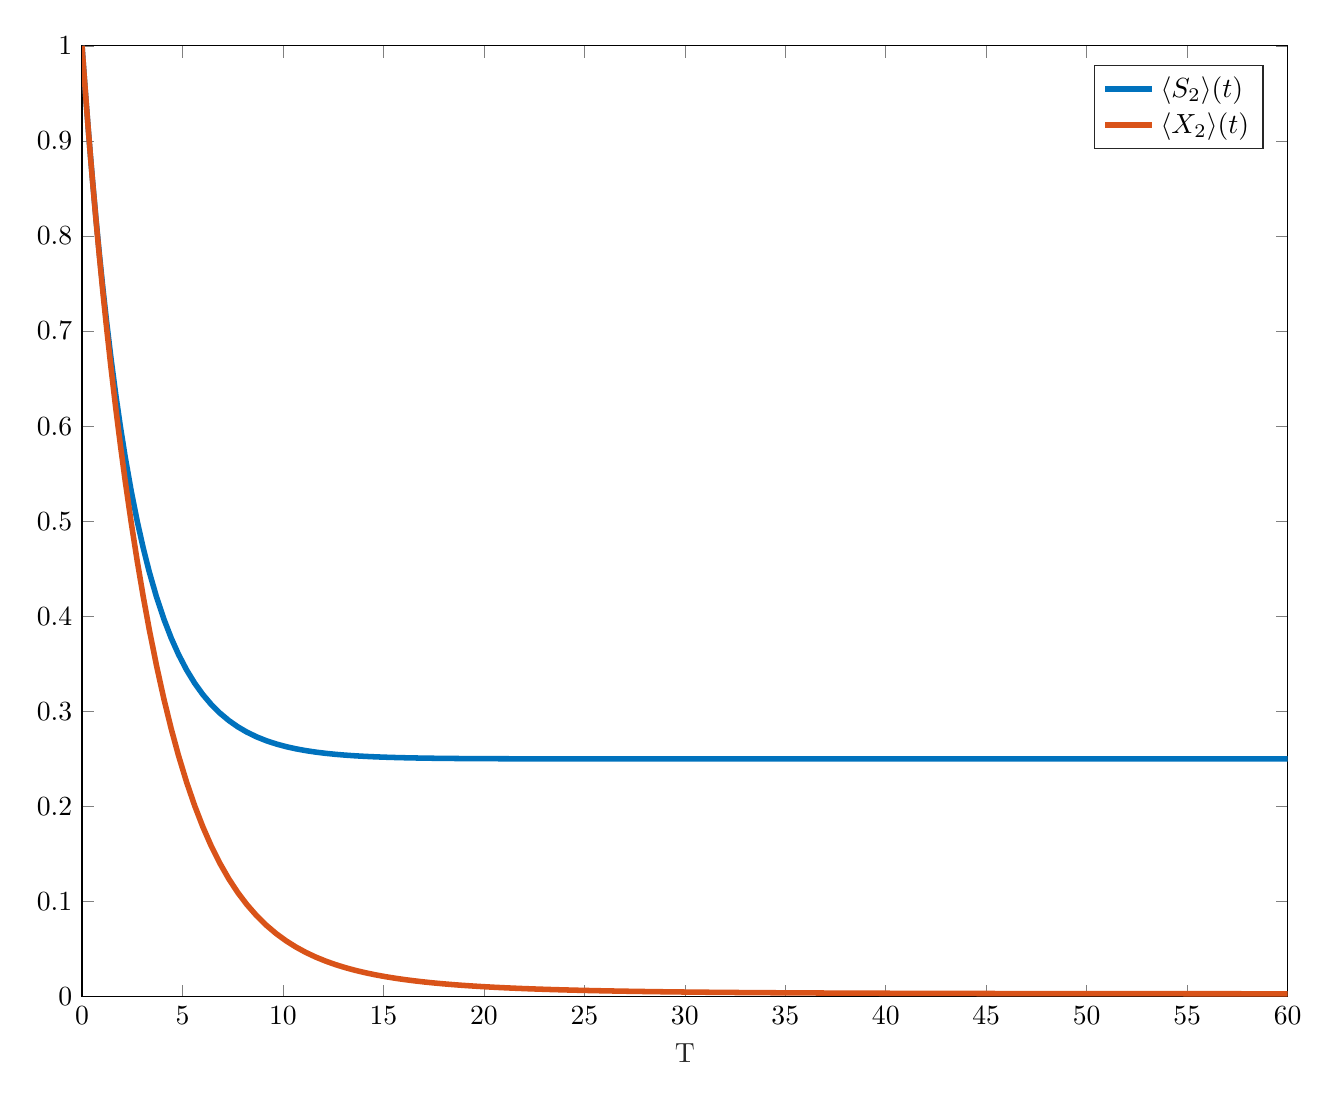
\begin{tikzpicture}

\begin{axis}[%
width=6.028in,
height=4.754in,
at={(1.011in,0.642in)},
scale only axis,
xmin=0,
xmax=60,
xlabel style={font=\color{white!15!black}},
xlabel={T},
ymin=0,
ymax=1,
axis background/.style={fill=white},
legend style={legend cell align=left, align=left, draw=white!15!black}
]
\addplot [color=mycolor1, line width=2.0pt]
  table[row sep=crcr]{%
0	1\\
0.000167459095433972	0.999949763953885\\
0.000334918190867944	0.999899531272651\\
0.000502377286301916	0.999849301956071\\
0.000669836381735888	0.999799076003922\\
0.00150713185890575	0.999547996701732\\
0.00234442733607561	0.999297001476487\\
0.00318172281324547	0.999046090300034\\
0.00401901829041533	0.998795263144227\\
0.00820549567626463	0.99754238669048\\
0.0123919730621139	0.996291606536599\\
0.0165784504479632	0.99504291917508\\
0.0207649278338125	0.993796321104278\\
0.041697314763059	0.987594547951493\\
0.0626297016923055	0.981444485184988\\
0.083562088621552	0.975345701651817\\
0.104494475550799	0.969297769768593\\
0.209156410197031	0.939806128919933\\
0.313818344843264	0.91152368113044\\
0.418480279489496	0.884400880611941\\
0.523142214135729	0.858390124885504\\
0.693500300195606	0.818313029330461\\
0.863858386255483	0.780876134190323\\
1.03421647231536	0.745905882432082\\
1.20457455837524	0.713239208200554\\
1.44051447786383	0.671518451609108\\
1.67645439735243	0.633555768395972\\
1.91239431684103	0.599014330293434\\
2.14833423632963	0.567583625933305\\
2.44722092525848	0.531792785970123\\
2.74610761418733	0.500036637585254\\
3.04499430311618	0.471864642818689\\
3.34388099204503	0.446867232882206\\
3.7078444355742	0.420187626925138\\
4.07180787910338	0.397125358000084\\
4.43577132263256	0.37719800996968\\
4.79973476616174	0.359970808884354\\
5.20292074647974	0.343584549055943\\
5.60610672679773	0.329641377827843\\
6.00929270711573	0.317785061805884\\
6.41247868743373	0.307695074640984\\
6.85758807700814	0.298279020146722\\
7.30269746658256	0.290400815197997\\
7.74780685615697	0.283816683396636\\
8.19291624573139	0.278306887206634\\
8.68220109096914	0.273270062909561\\
9.17148593620689	0.269130237284364\\
9.66077078144463	0.26573389992122\\
10.1500556266824	0.262941774813527\\
10.6416653734136	0.260629008549993\\
11.1332751201447	0.258729901399203\\
11.6248848668759	0.257173395775351\\
12.1164946136071	0.255894991586587\\
12.6079732666127	0.254841779768896\\
13.0994519196183	0.253976898623833\\
13.5909305726239	0.253268003848913\\
14.0824092256295	0.252685736828123\\
14.573895267778	0.252205890773349\\
15.0653813099266	0.251811849840116\\
15.5568673520752	0.251488877503596\\
16.0483533942238	0.251223597539249\\
16.5398390198718	0.251004984161706\\
17.0313246455198	0.250825462765357\\
17.5228102711679	0.250678319536887\\
18.0142958968159	0.250557460402728\\
18.5057815459406	0.250457862043894\\
18.9972671950653	0.250376073653432\\
19.48875284419	0.250309036475977\\
19.9802384933148	0.250253974104222\\
20.5017696853463	0.250206086979697\\
21.0233008773778	0.250167237410805\\
21.5448320694093	0.250135800555606\\
22.0663632614408	0.25011029017459\\
22.6746017709939	0.250086404450525\\
23.282840280547	0.250067696703614\\
23.8910787901001	0.250053130020746\\
24.4993172996532	0.25004171845769\\
25.0869400675273	0.250032958718024\\
25.6745628354014	0.250026040102264\\
26.2621856032755	0.250020602126255\\
26.8498083711495	0.250016305998746\\
27.5306427936611	0.250012399912303\\
28.2114772161728	0.25000943014995\\
28.8923116386844	0.25000719673085\\
29.573146061196	0.250005498735476\\
30.3571240725376	0.250004004549794\\
31.1411020838792	0.250002916085038\\
31.9250800952207	0.250002142131246\\
32.7090581065623	0.250001579100913\\
33.6393150845161	0.250001077720724\\
34.5695720624699	0.250000734525865\\
35.4998290404237	0.250000514703531\\
36.4300860183775	0.250000365483857\\
37.5675806203718	0.250000223876343\\
38.7050752223662	0.250000135575646\\
39.8425698243606	0.250000092288829\\
40.980064426355	0.250000066799481\\
42.4285780340909	0.250000031279727\\
43.8770916418269	0.250000012344854\\
45.3256052495628	0.250000011743775\\
46.7741188572988	0.250000013124446\\
48.2741188572988	0.25000000571389\\
49.7741188572988	0.250000001873181\\
51.2741188572988	0.250000002198961\\
52.7741188572988	0.250000002800139\\
54.2741188572988	0.250000001219075\\
55.7741188572988	0.250000000399649\\
57.2741188572988	0.250000000469155\\
58.7741188572988	0.250000000597418\\
59.0805891429741	0.250000000528484\\
59.3870594286494	0.250000000467506\\
59.6935297143247	0.250000000413576\\
60	0.250000000365868\\
};
\addlegendentry{$\langle\text{ S}_\text{2}\text{ }\rangle\text{(t)}$}

\addplot [color=mycolor2, line width=2.0pt]
  table[row sep=crcr]{%
0	1\\
0.000167459095433972	0.999949763953857\\
0.000334918190867944	0.999899531272425\\
0.000502377286301916	0.999849301955311\\
0.000669836381735888	0.999799076002119\\
0.00150713185890575	0.999547996681205\\
0.00234442733607561	0.999297001399249\\
0.00318172281324547	0.999046090107033\\
0.00401901829041533	0.998795262755379\\
0.00820549567626463	0.997542383386964\\
0.0123919730621139	0.996291595178081\\
0.0165784504479632	0.995042892025075\\
0.0207649278338125	0.993796267848315\\
0.041697314763059	0.987594120420592\\
0.0626297016923055	0.981443049142888\\
0.083562088621552	0.975342320785816\\
0.104494475550799	0.969291216183545\\
0.209156410197031	0.939755849652793\\
0.313818344843264	0.911360973769593\\
0.418480279489496	0.884031201510103\\
0.523142214135729	0.857698167570851\\
0.693500300195606	0.81680944243538\\
0.863858386255483	0.778163206698545\\
1.03421647231536	0.741557574425101\\
1.20457455837524	0.706819568750158\\
1.44051447786383	0.661520154084226\\
1.67645439735243	0.619190189816724\\
1.91239431684103	0.579558910208721\\
2.14833423632963	0.542402918667076\\
2.44722092525848	0.498599669712652\\
2.74610761418733	0.458157040342809\\
3.04499430311618	0.420813606357304\\
3.34388099204503	0.386345848519706\\
3.7078444355742	0.347972902082767\\
4.07180787910338	0.31325430231197\\
4.43577132263256	0.28189855399673\\
4.79973476616174	0.253633521758195\\
5.20292074647974	0.225620214495843\\
5.60610672679773	0.200753539499827\\
6.00929270711573	0.178721689929983\\
6.41247868743373	0.159232440119444\\
6.85758807700814	0.140343689946708\\
7.30269746658256	0.12388731981209\\
7.74780685615697	0.109559462335178\\
8.19291624573139	0.0970876854824286\\
8.68220109096914	0.0852318595654657\\
9.17148593620689	0.0750446855847971\\
9.66077078144463	0.0662821438209136\\
10.1500556266824	0.05873444568597\\
10.6416653734136	0.0521933804030884\\
11.1332751201447	0.0465424373231981\\
11.6248848668759	0.0416498643809277\\
12.1164946136071	0.037403972127709\\
12.6079732666127	0.0337111086868088\\
13.0994519196183	0.0304900896694505\\
13.5909305726239	0.0276732370812083\\
14.0824092256295	0.0252032509689746\\
14.573895267778	0.0230315494528747\\
15.0653813099266	0.0211169831688443\\
15.5568673520752	0.0194245619476555\\
16.0483533942238	0.0179245171666944\\
16.5398390198718	0.0165914776707145\\
17.0313246455198	0.0154037713069589\\
17.5228102711679	0.0143428582550358\\
18.0142958968159	0.0133928379709634\\
18.5057815459406	0.0125400450735501\\
18.9972671950653	0.0117727126576549\\
19.48875284419	0.0110806775888913\\
19.9802384933148	0.0104551522036236\\
20.5017696853463	0.00985562655117116\\
21.0233008773778	0.00931453062680311\\
21.5448320694093	0.00882504593325778\\
22.0663632614408	0.0083812721669376\\
22.6746017709939	0.00791465958461995\\
23.282840280547	0.00749626561710675\\
23.8910787901001	0.00712010602625066\\
24.4993172996532	0.00678105769059476\\
25.0869400675273	0.00648460726236425\\
25.6745628354014	0.00621525084903502\\
26.2621856032755	0.005970008377041\\
26.8498083711495	0.00574628074914531\\
27.5306427936611	0.00551099661871109\\
28.2114772161728	0.00529849326113302\\
28.8923116386844	0.00510613274889579\\
29.573146061196	0.00493163410296571\\
30.3571240725376	0.00475026671642952\\
31.1411020838792	0.00458737106367863\\
31.9250800952207	0.0044407235341731\\
32.7090581065623	0.00430841512066994\\
33.6393150845161	0.00416776865761866\\
34.5695720624699	0.00404265530493508\\
35.4998290404237	0.00393108663632639\\
36.4300860183775	0.00383137175427228\\
37.5675806203718	0.00372346054685316\\
38.7050752223662	0.00362889444570628\\
39.8425698243606	0.00354581178045761\\
40.980064426355	0.00347265037523595\\
42.4285780340909	0.00339178645080207\\
43.8770916418269	0.00332262732256281\\
45.3256052495628	0.00326332456346975\\
46.7741188572988	0.00321235771514442\\
48.2741188572988	0.00316702460979045\\
49.7741188572988	0.00312812143222317\\
51.2741188572988	0.00309468254080362\\
52.7741188572988	0.00306590043139326\\
54.2741188572988	0.00304109675586004\\
55.7741188572988	0.00301969934143004\\
57.2741188572988	0.00300122381818026\\
58.7741188572988	0.00298525882615117\\
59.0805891429741	0.00298227318141278\\
59.3870594286494	0.00297937483573661\\
59.6935297143247	0.00297656116518997\\
60	0.00297382963035769\\
};
\addlegendentry{$\langle\text{ X}_\text{2}\text{ }\rangle\text{ (t)}$}

\end{axis}
\end{tikzpicture}% 
	% This file was created by matlab2tikz.
%
\definecolor{mycolor1}{rgb}{0.00000,0.44700,0.74100}%
\definecolor{mycolor2}{rgb}{0.85000,0.32500,0.09800}%
%
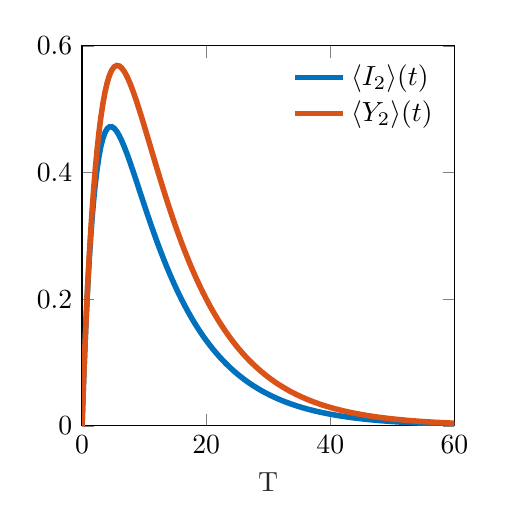
\begin{tikzpicture}

\begin{axis}[%
width=0.39\columnwidth,
height=1.9in,
at={(1.011in,0.642in)},
scale only axis,
xmin=0,
xmax=60,
xlabel style={font=\color{white!15!black}},
xlabel={T},
ymin=0,
ymax=0.6,
axis background/.style={fill=white},
legend style={legend cell align=left, align=left, draw=none,fill=none}
]
\addplot [color=mycolor1, line width=2.0pt]
  table[row sep=crcr]{%
0	0\\
0.000167459095433972	5.02356254883503e-05\\
0.000334918190867944	0.000100467044890239\\
0.000502377286301916	0.000150694258501483\\
0.000669836381735888	0.000200917266617879\\
0.00150713185890575	0.000451969235128613\\
0.00234442733607561	0.000702916110626103\\
0.00318172281324547	0.000953757930062376\\
0.00401901829041533	0.00120449473037694\\
0.00820549567626463	0.00245660473713581\\
0.0123919730621139	0.00370609479958259\\
0.0165784504479632	0.00495296952109098\\
0.0207649278338125	0.00619723349725102\\
0.041697314763059	0.0123795525149475\\
0.0626297016923055	0.0184972877685076\\
0.083562088621552	0.0245510050044134\\
0.104494475550799	0.0305412652287822\\
0.209156410197031	0.0595600686924977\\
0.313818344843264	0.0870738896256172\\
0.418480279489496	0.113147672208371\\
0.523142214135729	0.137843781066386\\
0.693500300195606	0.175249338581645\\
0.863858386255483	0.209405409857356\\
1.03421647231536	0.240538830760215\\
1.20457455837524	0.268862525001243\\
1.44051447786383	0.303818596471941\\
1.67645439735243	0.334245921772327\\
1.91239431684103	0.360582367596924\\
2.14833423632963	0.383230967745073\\
2.44722092525848	0.407198365602763\\
2.74610761418733	0.426485640869426\\
3.04499430311618	0.441672920138603\\
3.34388099204503	0.453286293297944\\
3.7078444355742	0.463275846874522\\
4.07180787910338	0.46935668981669\\
4.43577132263256	0.472139376138478\\
4.79973476616174	0.472172061936486\\
5.20292074647974	0.469567505094857\\
5.60610672679773	0.46467180684465\\
6.00929270711573	0.457921782162667\\
6.41247868743373	0.449708082295428\\
6.85758807700814	0.439335806446126\\
7.30269746658256	0.427911208540696\\
7.74780685615697	0.415715901892051\\
8.19291624573139	0.403001249816413\\
8.68220109096914	0.388671106840877\\
9.17148593620689	0.374149950243233\\
9.66077078144463	0.359594516257495\\
10.1500556266824	0.345144730282224\\
10.6416653734136	0.330843251166074\\
11.1332751201447	0.31682425223781\\
11.6248848668759	0.30314250445849\\
12.1164946136071	0.289845851051411\\
12.6079732666127	0.27697222726519\\
13.0994519196183	0.264532277469983\\
13.5909305726239	0.252536316282153\\
14.0824092256295	0.240992167355439\\
14.573895267778	0.229902115890175\\
15.0653813099266	0.219260240094611\\
15.5568673520752	0.209059232287995\\
16.0483533942238	0.199291195161469\\
16.5398390198718	0.189946340036884\\
17.0313246455198	0.181011536407207\\
17.5228102711679	0.172473590770781\\
18.0142958968159	0.164319488934899\\
18.5057815459406	0.156535802900637\\
18.9972671950653	0.14910805738424\\
19.48875284419	0.142022137868879\\
19.9802384933148	0.135264379521748\\
20.5017696853463	0.128437338075173\\
21.0233008773778	0.121948428479072\\
21.5448320694093	0.115782041394707\\
22.0663632614408	0.109923234113274\\
22.6746017709939	0.10345968067617\\
23.282840280547	0.0973725428757864\\
23.8910787901001	0.0916406186898327\\
24.4993172996532	0.0862438769737739\\
25.0869400675273	0.0813304947215163\\
25.6745628354014	0.0766957392759583\\
26.2621856032755	0.0723240733458858\\
26.8498083711495	0.068200783364252\\
27.5306427936611	0.0637157111733428\\
28.2114772161728	0.0595249505264587\\
28.8923116386844	0.0556093554280656\\
29.573146061196	0.051950953723168\\
30.3571240725376	0.0480350394326654\\
31.1411020838792	0.0444140402140323\\
31.9250800952207	0.0410658652957561\\
32.7090581065623	0.0379699469731079\\
33.6393150845161	0.0345974316000959\\
34.5695720624699	0.0315244003882625\\
35.4998290404237	0.0287244006816334\\
36.4300860183775	0.0261730527001414\\
37.5675806203718	0.0233588440636795\\
38.7050752223662	0.0208472681352205\\
39.8425698243606	0.0186060465411244\\
40.980064426355	0.0166057804025651\\
42.4285780340909	0.0143659448183652\\
43.8770916418269	0.0124283537428185\\
45.3256052495628	0.0107528736684299\\
46.7741188572988	0.00930335312641603\\
48.2741188572988	0.00800707471067509\\
49.7741188572988	0.00689150112952988\\
51.2741188572988	0.00593188939887653\\
52.7741188572988	0.00510596293416252\\
54.2741188572988	0.00439452344759861\\
55.7741188572988	0.00378226174883817\\
57.2741188572988	0.00325559841873243\\
58.7741188572988	0.00280230566423442\\
59.0805891429741	0.00271772603687272\\
59.3870594286494	0.00263569921449369\\
59.6935297143247	0.00255614817289934\\
60	0.00247899814359053\\
};
\addlegendentry{$\langle\text{ I}_\text{2}\text{ }\rangle\text{ (t)}$}

\addplot [color=mycolor2, line width=2.0pt]
  table[row sep=crcr]{%
0	0\\
0.000167459095433972	5.02356255165241e-05\\
0.000334918190867944	0.000100467045115613\\
0.000502377286301916	0.000150694259262062\\
0.000669836381735888	0.000200917268420599\\
0.00150713185890575	0.000451969255655102\\
0.00234442733607561	0.000702916187860346\\
0.00318172281324547	0.000953758123048095\\
0.00401901829041533	0.00120449511918631\\
0.00820549567626463	0.00245660803997705\\
0.0123919730621139	0.00370610615458687\\
0.0165784504479632	0.00495299665983842\\
0.0207649278338125	0.0061972867255334\\
0.041697314763059	0.0123799796075772\\
0.0626297016923055	0.0184987215786687\\
0.083562088621552	0.0245543787936758\\
0.104494475550799	0.0305478015879279\\
0.209156410197031	0.0596100683199002\\
0.313818344843264	0.0872352755037915\\
0.418480279489496	0.1135133727281\\
0.523142214135729	0.13852638857525\\
0.693500300195606	0.176725562555453\\
0.863858386255483	0.212056305065258\\
1.03421647231536	0.244767200155724\\
1.20457455837524	0.275073975429707\\
1.44051447786383	0.313422975959112\\
1.67645439735243	0.347943646809329\\
1.91239431684103	0.378992749240041\\
2.14833423632963	0.406871933412632\\
2.44722092525848	0.438037519492424\\
2.74610761418733	0.464975195482736\\
3.04499430311618	0.488066904527981\\
3.34388099204503	0.507646031039421\\
3.7078444355742	0.52717345030486\\
4.07180787910338	0.542415181193204\\
4.43577132263256	0.553810589679287\\
4.79973476616174	0.561764343985809\\
5.20292074647974	0.567010515859882\\
5.60610672679773	0.568966391920642\\
6.00929270711573	0.568067535257039\\
6.41247868743373	0.564713102425068\\
6.85758807700814	0.558593524173596\\
7.30269746658256	0.550362480383516\\
7.74780685615697	0.54040898211884\\
8.19291624573139	0.529074361767942\\
8.68220109096914	0.515373936774946\\
9.17148593620689	0.500700274220661\\
9.66077078144463	0.485337849105587\\
10.1500556266824	0.469524160995857\\
10.6416653734136	0.453379120670631\\
11.1332751201447	0.437140566465681\\
11.6248848668759	0.420941463771214\\
12.1164946136071	0.404888834318843\\
12.6079732666127	0.389072053748551\\
13.0994519196183	0.373553697130149\\
13.5909305726239	0.358385449135512\\
14.0824092256295	0.343606395048581\\
14.573895267778	0.329245001459219\\
15.0653813099266	0.315321618177901\\
15.5568673520752	0.301849360219801\\
16.0483533942238	0.288835620596475\\
16.5398390198718	0.27628316162386\\
17.0313246455198	0.264190983473947\\
17.5228102711679	0.252555090392891\\
18.0142958968159	0.24136910546898\\
18.5057815459406	0.230624777425767\\
18.9972671950653	0.220312399840216\\
19.48875284419	0.210421168130167\\
19.9802384933148	0.200939453944673\\
20.5017696853463	0.19131231472422\\
21.0233008773778	0.182117491735684\\
21.5448320694093	0.173339655520351\\
22.0663632614408	0.164963361661959\\
22.6746017709939	0.155681157696078\\
23.282840280547	0.146899954888701\\
23.8910787901001	0.138595994242475\\
24.4993172996532	0.130746073432756\\
25.0869400675273	0.123572286631831\\
25.6745628354014	0.11678159902841\\
26.2621856032755	0.110355047942582\\
26.8498083711495	0.104274367549387\\
27.5306427936611	0.0976386133862052\\
28.2114772161728	0.0914175980091737\\
28.8923116386844	0.0855865781167584\\
29.573146061196	0.0801220824785545\\
30.3571240725376	0.0742549188941794\\
31.1411020838792	0.0688124058708863\\
31.9250800952207	0.0637646639877352\\
32.7090581065623	0.0590837589691989\\
33.6393150845161	0.0539695326304018\\
34.5695720624699	0.0492947872074972\\
35.4998290404237	0.0450223790195588\\
36.4300860183775	0.0411181796559852\\
37.5675806203718	0.0367990869202093\\
38.7050752223662	0.0329317807381826\\
39.8425698243606	0.0294694424179177\\
40.980064426355	0.0263700045170798\\
42.4285780340909	0.0228891693906661\\
43.8770916418269	0.0198668481966104\\
45.3256052495628	0.0172429274273263\\
46.7741188572988	0.014965095315772\\
48.2741188572988	0.0129225931149068\\
49.7741188572988	0.01115863648395\\
51.2741188572988	0.00963532091069012\\
52.7741188572988	0.00831987518172544\\
54.2741188572988	0.00718397327506719\\
55.7741188572988	0.00620313644631283\\
57.2741188572988	0.00535621424249753\\
58.7741188572988	0.00462493465861914\\
59.0805891429741	0.00448828422601655\\
59.3870594286494	0.00435567233296861\\
59.6935297143247	0.0042269795528441\\
60	0.00410209004092822\\
};
\addlegendentry{$\langle\text{ Y}_\text{2}\text{ }\rangle\text{ (t)}$}

\end{axis}
\end{tikzpicture}%} 

\subfloat[][Nodo 3]{
	% This file was created by matlab2tikz.
%
\definecolor{mycolor1}{rgb}{0.00000,0.44700,0.74100}%
\definecolor{mycolor2}{rgb}{0.85000,0.32500,0.09800}%
%
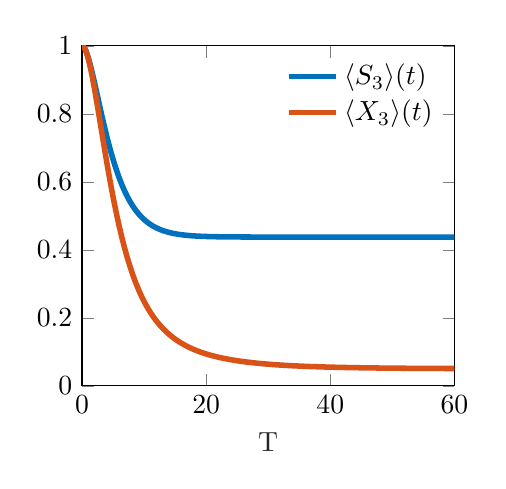
\begin{tikzpicture}

\begin{axis}[%
width=0.39\columnwidth,
height=1.7in,
at={(1.011in,0.642in)},
scale only axis,
xmin=0,
xmax=60,
xlabel style={font=\color{white!15!black}},
xlabel={T},
ymin=0,
ymax=1,
axis background/.style={fill=white},
legend style={legend cell align=left, align=left, draw=none,fill=none}
]
\addplot [color=mycolor1, line width=2.0pt]
  table[row sep=crcr]{%
0	1\\
0.000167459095433972	0.999999998738142\\
0.000334918190867944	0.999999994952792\\
0.000502377286301916	0.999999988644289\\
0.000669836381735888	0.999999979812971\\
0.00150713185890575	0.999999897825981\\
0.00234442733607561	0.999999752819296\\
0.00318172281324547	0.99999954483513\\
0.00401901829041533	0.999999273915676\\
0.00820549567626463	0.999996976764418\\
0.0123919730621139	0.999993112547874\\
0.0165784504479632	0.999987686516463\\
0.0207649278338125	0.999980703907444\\
0.041697314763059	0.999922624618094\\
0.0626297016923055	0.999826408925982\\
0.083562088621552	0.99969269680636\\
0.104494475550799	0.999522120290137\\
0.209156410197031	0.998137960827395\\
0.313818344843264	0.995922465165433\\
0.418480279489496	0.992946027807028\\
0.523142214135729	0.989274937612289\\
0.693500300195606	0.981973940722739\\
0.863858386255483	0.973240038754978\\
1.03421647231536	0.963292530931682\\
1.20457455837524	0.952330841025336\\
1.44051447786383	0.935806342228975\\
1.67645439735243	0.918080997911094\\
1.91239431684103	0.899500127085142\\
2.14833423632963	0.880367859680095\\
2.44722092525848	0.85574171145015\\
2.74610761418733	0.83103916350853\\
3.04499430311618	0.806578409348801\\
3.34388099204503	0.782631978004113\\
3.7078444355742	0.75447211159862\\
4.07180787910338	0.727603684649032\\
4.43577132263256	0.702174223241644\\
4.79973476616174	0.678307316278175\\
5.20292074647974	0.653774724370522\\
5.60610672679773	0.631205361841917\\
6.00929270711573	0.610542558139064\\
6.41247868743373	0.591735043728731\\
6.85758807700814	0.57303680236404\\
7.30269746658256	0.556333540005082\\
7.74780685615697	0.541460456252127\\
8.19291624573139	0.528275695887157\\
8.68220109096914	0.51556125386222\\
9.17148593620689	0.504497996616038\\
9.66077078144463	0.494894174784991\\
10.1500556266824	0.486586354120359\\
10.6416653734136	0.479392347597474\\
11.1332751201447	0.473202420173063\\
11.6248848668759	0.46788601528397\\
12.1164946136071	0.463329681682318\\
12.6079732666127	0.459433513843843\\
13.0994519196183	0.456105361253136\\
13.5909305726239	0.453266757288285\\
14.0824092256295	0.450848775743308\\
14.573895267778	0.44879122631073\\
15.0653813099266	0.447042976012409\\
15.5568673520752	0.445559600087142\\
16.0483533942238	0.444301821295448\\
16.5398390198718	0.443235739886372\\
17.0313246455198	0.442333582646524\\
17.5228102711679	0.441571158188601\\
18.0142958968159	0.440926985076838\\
18.5057815459406	0.440382661675318\\
18.9972671950653	0.439923504076921\\
19.48875284419	0.439536690438452\\
19.9802384933148	0.439210799744039\\
20.5017696853463	0.438920754658941\\
21.0233008773778	0.438679302761171\\
21.5448320694093	0.438478627706432\\
22.0663632614408	0.43831175482993\\
22.6746017709939	0.438152012143916\\
23.282840280547	0.438023420740633\\
23.8910787901001	0.437920237430922\\
24.4993172996532	0.437837273729477\\
25.0869400675273	0.437772357070206\\
25.6745628354014	0.437719844553824\\
26.2621856032755	0.437677488337093\\
26.8498083711495	0.437643254426811\\
27.5306427936611	0.437611553445292\\
28.2114772161728	0.437586827964751\\
28.8923116386844	0.437567662580957\\
29.573146061196	0.437552729805634\\
30.3571240725376	0.437539406333623\\
31.1411020838792	0.43752943285221\\
31.9250800952207	0.437522069969169\\
32.7090581065623	0.437516567914547\\
33.6393150845161	0.437511657612987\\
34.5695720624699	0.437508192616622\\
35.4998290404237	0.437505840190485\\
36.4300860183775	0.437504189241777\\
37.5675806203718	0.437502680495585\\
38.7050752223662	0.437501704404973\\
39.8425698243606	0.437501154963458\\
40.980064426355	0.437500810027397\\
42.4285780340909	0.437500423216806\\
43.8770916418269	0.437500205882951\\
45.3256052495628	0.437500155093005\\
46.7741188572988	0.437500139033043\\
48.2741188572988	0.437500070492889\\
49.7741188572988	0.437500032582013\\
51.2741188572988	0.437500025442845\\
52.7741188572988	0.437500024043849\\
54.2741188572988	0.437500012593451\\
55.7741188572988	0.437500006149462\\
57.2741188572988	0.437500004486816\\
58.7741188572988	0.43750000393094\\
59.0805891429741	0.437500003525987\\
59.3870594286494	0.437500003162157\\
59.6935297143247	0.437500002835375\\
60	0.437500002541907\\
};
\addlegendentry{$\langle\text{ S}_\text{3}\text{ }\rangle\text{(t)}$}

\addplot [color=mycolor2, line width=2.0pt]
  table[row sep=crcr]{%
0	1\\
0.000167459095433972	0.999999998738121\\
0.000334918190867944	0.999999994952623\\
0.000502377286301916	0.999999988643719\\
0.000669836381735888	0.999999979811619\\
0.00150713185890575	0.999999897810584\\
0.00234442733607561	0.999999752761357\\
0.00318172281324547	0.999999544690347\\
0.00401901829041533	0.999999273623959\\
0.00820549567626463	0.999996974285392\\
0.0123919730621139	0.99999310402177\\
0.0165784504479632	0.999987666130806\\
0.0207649278338125	0.999980663908501\\
0.041697314763059	0.999922303080207\\
0.0626297016923055	0.999825327388393\\
0.083562088621552	0.999690146760756\\
0.104494475550799	0.999517169946184\\
0.209156410197031	0.998099562083633\\
0.313818344843264	0.995797602736572\\
0.418480279489496	0.992660787241997\\
0.523142214135729	0.988737569824434\\
0.693500300195606	0.980791887673879\\
0.863858386255483	0.971084816672113\\
1.03421647231536	0.959804485451343\\
1.20457455837524	0.947129575840581\\
1.44051447786383	0.92758521760773\\
1.67645439735243	0.906106445832667\\
1.91239431684103	0.883075108589426\\
2.14833423632963	0.858837590253955\\
2.44722092525848	0.826886007743043\\
2.74610761418733	0.794054411348015\\
3.04499430311618	0.760820010065433\\
3.34388099204503	0.727585063894323\\
3.7078444355742	0.687591104586465\\
4.07180787910338	0.648565972587078\\
4.43577132263256	0.610869108045145\\
4.79973476616174	0.574757882885561\\
5.20292074647974	0.536811750289604\\
5.60610672679773	0.501154822235437\\
6.00929270711573	0.46783841094304\\
6.41247868743373	0.436850883694166\\
6.85758807700814	0.405275435185886\\
7.30269746658256	0.376344399323862\\
7.74780685615697	0.349904623141994\\
8.19291624573139	0.325786226657295\\
8.68220109096914	0.301742096377738\\
9.17148593620689	0.280056160791516\\
9.66077078144463	0.260503229035094\\
10.1500556266824	0.242871160246053\\
10.6416653734136	0.226891693201811\\
11.1332751201447	0.212470740859802\\
11.6248848668759	0.199443155444072\\
12.1164946136071	0.187660352686063\\
12.6079732666127	0.176992040603435\\
13.0994519196183	0.167316401231543\\
13.5909305726239	0.15852801642726\\
14.0824092256295	0.150533283579751\\
14.573895267778	0.143249079022458\\
15.0653813099266	0.136601930856374\\
15.5568673520752	0.130526600867737\\
16.0483533942238	0.124965248309587\\
16.5398390198718	0.119866568704441\\
17.0313246455198	0.115185000892432\\
17.5228102711679	0.110880064930525\\
18.0142958968159	0.106915746746887\\
18.5057815459406	0.103259964703636\\
18.9972671950653	0.0998841105748442\\
19.48875284419	0.0967626241214158\\
19.9802384933148	0.093872652366401\\
20.5017696853463	0.0910363694187017\\
21.0233008773778	0.0884158587940551\\
21.5448320694093	0.0859915788622176\\
22.0663632614408	0.0837460650816602\\
22.6746017709939	0.0813322583853868\\
23.282840280547	0.0791182798112997\\
23.8910787901001	0.0770846044770127\\
24.4993172996532	0.0752139465164833\\
25.0869400675273	0.0735470960341475\\
25.6745628354014	0.0720057390561177\\
26.2621856032755	0.0705788449983809\\
26.8498083711495	0.0692565149973051\\
27.5306427936611	0.06784353618056\\
28.2114772161728	0.066546673051544\\
28.8923116386844	0.0653549652901753\\
29.573146061196	0.0642586554629632\\
30.3571240725376	0.063103159557281\\
31.1411020838792	0.0620508751398579\\
31.9250800952207	0.0610914208358915\\
32.7090581065623	0.0602156212256792\\
33.6393150845161	0.0592737881763883\\
34.5695720624699	0.0584263864507068\\
35.4998290404237	0.0576629977791319\\
36.4300860183775	0.0569745079611135\\
37.5675806203718	0.0562228313805171\\
38.7050752223662	0.0555585438870261\\
39.8425698243606	0.0549707401692344\\
40.980064426355	0.0544500217669509\\
42.4285780340909	0.0538713152654743\\
43.8770916418269	0.0533739986675399\\
45.3256052495628	0.0529460801788547\\
46.7741188572988	0.0525774669931346\\
48.2741188572988	0.0522491769173989\\
49.7741188572988	0.0519673459336875\\
51.2741188572988	0.0517252105971922\\
52.7741188572988	0.0515170392194709\\
54.2741188572988	0.0513379628371783\\
55.7741188572988	0.0511838366660678\\
57.2741188572988	0.0510511258845694\\
58.7741188572988	0.0509368110338632\\
59.0805891429741	0.0509154776538754\\
59.3870594286494	0.0508947831556744\\
59.6935297143247	0.050874708138684\\
60	0.0508552338163797\\
};
\addlegendentry{$\langle\text{ X}_\text{3}\text{ }\rangle\text{ (t)}$}

\end{axis}
\end{tikzpicture}%
	% This file was created by matlab2tikz.
%
\definecolor{mycolor1}{rgb}{0.00000,0.44700,0.74100}%
\definecolor{mycolor2}{rgb}{0.85000,0.32500,0.09800}%
%
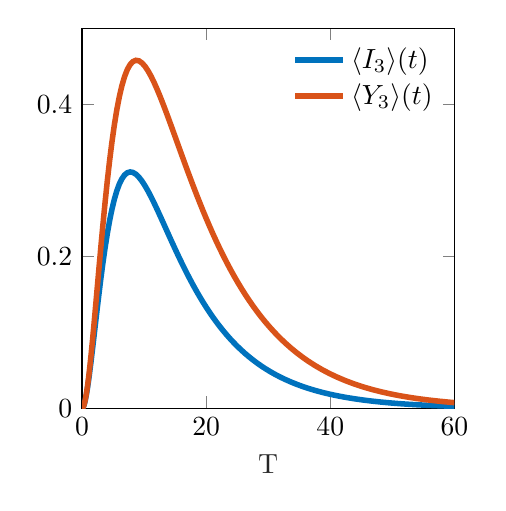
\begin{tikzpicture}

\begin{axis}[%
width=0.39\columnwidth,
height=1.9in,
at={(1.011in,0.642in)},
scale only axis,
xmin=0,
xmax=60,
xlabel style={font=\color{white!15!black}},
xlabel={T},
ymin=0,
ymax=0.5,
axis background/.style={fill=white},
legend style={legend cell align=left, align=left, draw=none,fill=none}
]
\addplot [color=mycolor1, line width=2.0pt]
  table[row sep=crcr]{%
0	0\\
0.000167459095433972	1.26185129491217e-09\\
0.000334918190867944	5.04715161691134e-09\\
0.000502377286301916	1.13555206521399e-08\\
0.000669836381735888	2.01865781270714e-08\\
0.00150713185890575	1.02168885342488e-07\\
0.00234442733607561	2.47161385709955e-07\\
0.00318172281324547	4.55116590395451e-07\\
0.00401901829041533	7.25987035736679e-07\\
0.00820549567626463	3.02240839189113e-06\\
0.0123919730621139	6.88460568276832e-06\\
0.0165784504479632	1.23066742198438e-05\\
0.0207649278338125	1.92827249369075e-05\\
0.041697314763059	7.7267642315786e-05\\
0.0626297016923055	0.000173227718853331\\
0.083562088621552	0.000306444247749785\\
0.104494475550799	0.000476207943859229\\
0.209156410197031	0.00184891650923723\\
0.313818344843264	0.00403428386881361\\
0.418480279489496	0.00695384907760906\\
0.523142214135729	0.0105339891355051\\
0.693500300195606	0.0175971136151213\\
0.863858386255483	0.0259614923743754\\
1.03421647231536	0.0353880052833885\\
1.20457455837524	0.0456606118346815\\
1.44051447786383	0.0609285917757482\\
1.67645439735243	0.0770270262868401\\
1.91239431684103	0.0935965284435017\\
2.14833423632963	0.110324114104919\\
2.44722092525848	0.13133553630602\\
2.74610761418733	0.151803393776639\\
3.04499430311618	0.17143301715889\\
3.34388099204503	0.189977555508\\
3.7078444355742	0.210833991668167\\
4.07180787910338	0.229677134951398\\
4.43577132263256	0.246438421785966\\
4.79973476616174	0.261066449116606\\
5.20292074647974	0.274785754990105\\
5.60610672679773	0.286039368883271\\
6.00929270711573	0.294983433116465\\
6.41247868743373	0.30175643196477\\
6.85758807700814	0.306899090107461\\
7.30269746658256	0.309867303731916\\
7.74780685615697	0.310918643619185\\
8.19291624573139	0.310273875840171\\
8.68220109096914	0.307859497934145\\
9.17148593620689	0.30394952537288\\
9.66077078144463	0.298802849798728\\
10.1500556266824	0.292638032935273\\
10.6416653734136	0.285615796252768\\
11.1332751201447	0.277950926739595\\
11.6248848668759	0.269801213188547\\
12.1164946136071	0.261301267061574\\
12.6079732666127	0.252569321908963\\
13.0994519196183	0.243702027756301\\
13.5909305726239	0.234781977080018\\
14.0824092256295	0.225879536525819\\
14.573895267778	0.217053038249217\\
15.0653813099266	0.208348121918181\\
15.5568673520752	0.199801976342069\\
16.0483533942238	0.191445697640121\\
16.5398390198718	0.183303671016761\\
17.0313246455198	0.175392222310533\\
17.5228102711679	0.167723699389534\\
18.0142958968159	0.160307635901842\\
18.5057815459406	0.153150116044107\\
18.9972671950653	0.146252792268445\\
19.48875284419	0.139615587093586\\
19.9802384933148	0.133237287300585\\
20.5017696853463	0.126749085509615\\
21.0233008773778	0.120543262208316\\
21.5448320694093	0.114613005008405\\
22.0663632614408	0.108951184514624\\
22.6746017709939	0.102676735601474\\
23.282840280547	0.0967423452585563\\
23.8910787901001	0.0911334321360161\\
24.4993172996532	0.0858358971254951\\
25.0869400675273	0.0810003106792662\\
25.6745628354014	0.0764286533064571\\
26.2621856032755	0.0721080243560162\\
26.8498083711495	0.0680260834605836\\
27.5306427936611	0.0635793731585896\\
28.2114772161728	0.0594186100567405\\
28.8923116386844	0.0555263353843065\\
29.573146061196	0.0518861460511328\\
30.3571240725376	0.0479865022042955\\
31.1411020838792	0.0443777124961245\\
31.9250800952207	0.0410385808014444\\
32.7090581065623	0.0379494355212916\\
33.6393150845161	0.0345829658368376\\
34.5695720624699	0.0315142114252991\\
35.4998290404237	0.0287171284645176\\
36.4300860183775	0.0261678325282954\\
37.5675806203718	0.0233554939459096\\
38.7050752223662	0.0208451311709022\\
39.8425698243606	0.0186045988786763\\
40.980064426355	0.0166047671655161\\
42.4285780340909	0.0143654118090185\\
43.8770916418269	0.0124280915770715\\
45.3256052495628	0.0107526786215321\\
46.7741188572988	0.00930318087347226\\
48.2741188572988	0.00800698643404652\\
49.7741188572988	0.00689145956002702\\
51.2741188572988	0.00593185767404391\\
52.7741188572988	0.00510593367583665\\
54.2741188572988	0.00439450787540565\\
55.7741188572988	0.00378225394920435\\
57.2741188572988	0.00325559290546576\\
58.7741188572988	0.00280230102039895\\
59.0805891429741	0.00271772186404062\\
59.3870594286494	0.00263569546579028\\
59.6935297143247	0.00255614480597557\\
60	0.00247899512024932\\
};
\addlegendentry{$\langle\text{ I}_\text{3}\text{ }\rangle\text{ (t)}$}

\addplot [color=mycolor2, line width=2.0pt]
  table[row sep=crcr]{%
0	0\\
0.000167459095433972	1.26187242549581e-09\\
0.000334918190867944	5.04732065095519e-09\\
0.000502377286301916	1.13560911062091e-08\\
0.000669836381735888	2.01879302295867e-08\\
0.00150713185890575	1.02184281803407e-07\\
0.00234442733607561	2.47219320713395e-07\\
0.00318172281324547	4.55261361324533e-07\\
0.00401901829041533	7.26278723323254e-07\\
0.00820549567626463	3.02488691034271e-06\\
0.0123919730621139	6.89312914165404e-06\\
0.0165784504479632	1.23270514159998e-05\\
0.0207649278338125	1.93227030901108e-05\\
0.041697314763059	7.75888461837317e-05\\
0.0626297016923055	0.00017430755083688\\
0.083562088621552	0.000308988928504255\\
0.104494475550799	0.000481145277362125\\
0.209156410197031	0.00188713998878568\\
0.313818344843264	0.00415819235297196\\
0.418480279489496	0.00723605935851084\\
0.523142214135729	0.0110641401707356\\
0.693500300195606	0.0187582501128445\\
0.863858386255483	0.0280685939090168\\
1.03421647231536	0.038781348702539\\
1.20457455837524	0.050695670725046\\
1.44051447786383	0.0688333053117084\\
1.67645439735243	0.0884590045160488\\
1.91239431684103	0.109160760888305\\
2.14833423632963	0.130571221115777\\
2.44722092525848	0.158207981143474\\
2.74610761418733	0.185896662878587\\
3.04499430311618	0.213165780463282\\
3.34388099204503	0.239631557052223\\
3.7078444355742	0.270339304796926\\
4.07180787910338	0.298996850299779\\
4.43577132263256	0.325324823585313\\
4.79973476616174	0.349154022298033\\
5.20292074647974	0.372540604911139\\
5.60610672679773	0.392759067286727\\
6.00929270711573	0.409884549124148\\
6.41247868743373	0.424050853489826\\
6.85758807700814	0.436463050104125\\
7.30269746658256	0.445748970833454\\
7.74780685615697	0.452194594924938\\
8.19291624573139	0.456089769321328\\
8.68220109096914	0.457766673464304\\
9.17148593620689	0.457062988320793\\
9.66077078144463	0.454312115034089\\
10.1500556266824	0.449818784655169\\
10.6416653734136	0.443826478157626\\
11.1332751201447	0.436601503850688\\
11.6248848668759	0.428364081717156\\
12.1164946136071	0.419307707507557\\
12.6079732666127	0.409604053214299\\
13.0994519196183	0.399397555767262\\
13.5909305726239	0.388815151472685\\
14.0824092256295	0.377966163528239\\
14.573895267778	0.366944181775427\\
15.0653813099266	0.355829440028067\\
15.5568673520752	0.344690017892647\\
16.0483533942238	0.333583512446607\\
16.5398390198718	0.322558397412516\\
17.0313246455198	0.311655195698201\\
17.5228102711679	0.300907540097816\\
18.0142958968159	0.290343098921674\\
18.5057815459406	0.279984375468896\\
18.9972671950653	0.269849406585556\\
19.48875284419	0.259952393792112\\
19.9802384933148	0.25030421247411\\
20.5017696853463	0.240347267136109\\
21.0233008773778	0.23068614253712\\
21.5448320694093	0.221324840198831\\
22.0663632614408	0.212265130705681\\
22.6746017709939	0.20207997883171\\
23.282840280547	0.192302092044039\\
23.8910787901001	0.182926369836573\\
24.4993172996532	0.173945839215214\\
25.0869400675273	0.165637103962906\\
25.6745628354014	0.157680717688887\\
26.2621856032755	0.150067281055099\\
26.8498083711495	0.142786828909496\\
27.5306427936611	0.134754242803134\\
28.2114772161728	0.127138152884103\\
28.8923116386844	0.119921737176536\\
29.573146061196	0.113088113835243\\
30.3571240725376	0.105671559434967\\
31.1411020838792	0.0987150371633935\\
31.9250800952207	0.0921938384173302\\
32.7090581065623	0.0860839551570198\\
33.6393150845161	0.0793357364963272\\
34.5695720624699	0.0730968726927723\\
35.4998290404237	0.0673320550305249\\
36.4300860183775	0.062007867055897\\
37.5675806203718	0.0560505407170007\\
38.7050752223662	0.0506512402712961\\
39.8425698243606	0.045760260874588\\
40.980064426355	0.0413318198027856\\
42.4285780340909	0.0362960168768387\\
43.8770916418269	0.0318636645068222\\
45.3256052495628	0.0279645282209824\\
46.7741188572988	0.0245360808627083\\
48.2741188572988	0.0214226728395207\\
49.7741188572988	0.018699880307068\\
51.2741188572988	0.0163195611727412\\
52.7741188572988	0.0142393231839026\\
54.2741188572988	0.0124218796892963\\
55.7741188572988	0.0108344668021829\\
57.2741188572988	0.00944831909937817\\
58.7741188572988	0.00823820038111376\\
59.0805891429741	0.0080105617745301\\
59.3870594286494	0.00778916478021219\\
59.6935297143247	0.00757383996796787\\
60	0.0073644224945157\\
};
\addlegendentry{$\langle\text{ Y}_\text{3}\text{ }\rangle\text{ (t)}$}

\end{axis}
\end{tikzpicture}%}
\\
\phantomcaption
\end{figure}
\begin{figure}[t]
\ContinuedFloat
\centering
\subfloat[][Prevalenza.]
{% This file was created by matlab2tikz.
%
%The latest updates can be retrieved from
%  http://www.mathworks.com/matlabcentral/fileexchange/22022-matlab2tikz-matlab2tikz
%where you can also make suggestions and rate matlab2tikz.
%
\begin{tikzpicture}

\begin{axis}[%
width=6.028in,
height=4.754in,
at={(1.011in,0.642in)},
scale only axis,
xmin=0,
xmax=5,
ymin=0,
ymax=0.35,
axis background/.style={fill=white},
axis x line*=bottom,
axis y line*=left,
legend style={legend cell align=left, align=left, draw=white!15!black}
]
\addplot [color=red, line width=2.0pt]
  table[row sep=crcr]{%
0	0.333333333333333\\
0.000100475457260383	0.333327750896148\\
0.000200950914520766	0.333322167524441\\
0.00030142637178115	0.333316583218443\\
0.000401901829041533	0.333310997978383\\
0.000904279115343449	0.333283057775202\\
0.00140665640164536	0.333255094254932\\
0.00190903368794728	0.333227107446242\\
0.0024114109742492	0.333199097377757\\
0.00492329740575878	0.333058699137463\\
0.00743518383726836	0.332917723672439\\
0.00994707026877794	0.332776174514818\\
0.0124589567002875	0.332634055171426\\
0.0250183888578354	0.331915026764786\\
0.0375778210153833	0.331182255384855\\
0.0501372531729312	0.330436152327952\\
0.0626966853304791	0.329677114738795\\
0.102108236390274	0.327215481818432\\
0.141519787450068	0.324641174996368\\
0.180931338509863	0.321964171028335\\
0.220342889569658	0.31919350535293\\
0.274870838360705	0.315220730809272\\
0.329398787151753	0.311103336256022\\
0.383926735942801	0.306858491220908\\
0.438454684733849	0.302501546535542\\
0.511698843017727	0.296496384111662\\
0.584943001301606	0.290342511122817\\
0.658187159585485	0.284066091588779\\
0.731431317869363	0.277690592664632\\
0.823962581336954	0.269526726473224\\
0.916493844804545	0.261275455659342\\
1.00902510827214	0.252971216615607\\
1.10155637173973	0.244645176809034\\
1.21569652246265	0.23438574594883\\
1.32983667318558	0.224183113794988\\
1.44397682390851	0.214080766948463\\
1.55811697463144	0.204117072879612\\
1.68311697463144	0.193403784285744\\
1.80811697463144	0.182936514271466\\
1.93311697463144	0.172749616737409\\
2.05811697463144	0.162871139436702\\
2.18311697463144	0.153323565735268\\
2.30811697463144	0.144126198180392\\
2.43311697463144	0.135293531088611\\
2.55811697463144	0.126835090981413\\
2.68311697463144	0.118756329228822\\
2.80811697463144	0.11106042130276\\
2.93311697463144	0.10374712141988\\
3.05811697463144	0.0968128382965037\\
3.18311697463144	0.0902514673020522\\
3.30811697463144	0.0840557450763619\\
3.43311697463144	0.0782164406459592\\
3.55811697463144	0.0727224755499841\\
3.68311697463144	0.0675615941436991\\
3.80811697463144	0.0627213396997781\\
3.93311697463144	0.0581884346441867\\
4.05811697463144	0.0539488620496409\\
4.18311697463144	0.0499883521752367\\
4.30811697463144	0.0462930527442834\\
4.43311697463144	0.0428490255007505\\
4.55811697463144	0.0396422733863442\\
4.66858773097358	0.0369947840804212\\
4.77905848731572	0.034512898505142\\
4.88952924365786	0.0321877719670461\\
5	0.0300107450038088\\
};
\addlegendentry{Approssimata}

\addplot [color=blue, line width=2.0pt]
  table[row sep=crcr]{%
0	0.333333333333333\\
0.000100475457260383	0.33332775117652\\
0.000200950914520766	0.333322168645711\\
0.00030142637178115	0.333316585740814\\
0.000401901829041533	0.333311002461736\\
0.000904279115343449	0.333283080450326\\
0.00140665640164536	0.333255149070309\\
0.00190903368794728	0.333227208309998\\
0.0024114109742492	0.333199258157732\\
0.00492329740575878	0.333059366110503\\
0.00743518383726836	0.332919237528702\\
0.00994707026877794	0.332778870981109\\
0.0124589567002875	0.332638265051006\\
0.0250183888578354	0.331931595902953\\
0.0375778210153833	0.331218738109183\\
0.0501372531729312	0.330499530838155\\
0.0626966853304791	0.329773821516115\\
0.0991412937643315	0.327629833725129\\
0.135585902198184	0.32542682709702\\
0.172030510632036	0.323162271980266\\
0.208475119065889	0.320834051099024\\
0.257093885813804	0.317626142783061\\
0.305712652561719	0.314299781871326\\
0.354331419309635	0.310853927218438\\
0.40295018605755	0.307288328954497\\
0.46627950019307	0.302465571513947\\
0.52960881432859	0.297446337787991\\
0.592938128464109	0.292238061528472\\
0.656267442599629	0.286849067385365\\
0.733658471248229	0.280032591279204\\
0.811049499896829	0.272984735524843\\
0.888440528545428	0.265730903942892\\
0.965831557194028	0.258296309197627\\
1.05793596976172	0.249249184589584\\
1.15004038232942	0.240033136540703\\
1.24214479489711	0.230697304828548\\
1.3342492074648	0.221287878081579\\
1.44286725998794	0.210158037529048\\
1.55148531251107	0.199063059012029\\
1.66010336503421	0.188071612582134\\
1.76872141755734	0.177244701902424\\
1.88893196521442	0.165520374303466\\
2.00914251287149	0.154131833198533\\
2.12935306052856	0.143134740860959\\
2.24956360818563	0.132574608346779\\
2.37456360818563	0.12209553959032\\
2.49956360818563	0.112155781376778\\
2.62456360818563	0.102773341814187\\
2.74956360818563	0.0939584472228666\\
2.87456360818563	0.0857132435851595\\
2.99956360818563	0.0780307810161572\\
3.12456360818563	0.0708988244967405\\
3.24956360818563	0.0643015118334588\\
3.37456360818563	0.0582191503589672\\
3.49956360818563	0.0526277151834682\\
3.62456360818563	0.0475016394160471\\
3.74956360818563	0.0428146697023513\\
3.87456360818563	0.0385398175357336\\
3.99956360818563	0.0346492430664406\\
4.12456360818563	0.031115623106694\\
4.24956360818563	0.0279124562820615\\
4.37456360818563	0.0250140892127293\\
4.49956360818563	0.0223957818462954\\
4.62456360818563	0.0200340851137771\\
4.74956360818563	0.0179068527747512\\
4.81217270613922	0.0169229578724849\\
4.87478180409282	0.015990178489161\\
4.93739090204641	0.0151061256192865\\
5	0.0142684938646879\\
};
\addlegendentry{Esatta}

\end{axis}
\end{tikzpicture}%}
\caption[Confronto tra modello esatto e chiuso alle coppie per~\ref{fig::3nodi}]{Divisione in classi dei  singoli nodi (a)(b) e grafico della prevalenza~(c). Non abbiamo riportato i grafici relativi al nodo $1$ poich\'e in questo caso il modello esatto e il modello chiuso alle coppie coincidono. Per ottenere i grafici abbiamo risolto numericamente,  usando MATLAB,  il problema di Cauchy derivato dal modello esatto~\eqref{3nodi} (in blu) e quello approssimato  ottenuto   assumendo la chiusura alle coppie~\eqref{Chiuso_coppie} (in rosso).  Per entrambi i modelli le condizioni iniziali sono stati puri~\eqref{statipuri}, inoltre,  nel modello esatto abbiamo supposto l'indipendenza statistica di tali condizioni iniziali. Per la sperimentazione abbiamo usato come parametri $\tau=0.3$ e $\gamma=0.1$.\\}
\label{fig::coppie3nodi}
\end{figure}

\subsection{Chiusura al livello delle triple}
In analogia a quanto fatto nel paragrafo precedente, cercheremo di sfruttare l'indipendenza a livello delle triple ovvero l'approssimazione
$$ \angol{ A_i B_j C_k }\approx \frac{\angol{A_iB_j}\angol{B_jC_k}}{\angol{B_j}}$$
 per ottenere un modello chiuso (con un numero minore di equazioni rispetto a quello esatto). Tale modello ci fornir\`a  un'approssimazione migliore di quello chiuso ottenuto assumendo l'indipendenza a livello delle coppie.\\ \\
Come nel caso delle coppie, per rimarcare la non esattezza del modello useremo le lettere $X,Y$ al posto di $S$ e $I$. \\
Nel  modello esatto, per i singoli nodi vale: \begin{equation*}
\begin{aligned}
	\dot{\angol{S_i}} = &-\tau \sum_{j=1\atop {j\neq i }} ^N g_{ij} \angol{S_i I_j},\\
	\dot{\angol{I_i}} = &\spa\tau \sum_{j=1\atop {j\neq i }} ^N g_{ij} \angol{S_i I_j} -\gamma \angol{I_i}.
\end{aligned}
\end{equation*}
Mentre per le coppie 
$$
\dot{\angol{S_i I_j}} = \tau \sum_{k=1\atop{k\neq i }}^N g_{jk} \angol{S_iS_jI_k} - \tau \sum_{k=1\atop{k\neq j }}^N g_{ik} \angol{I_kS_iI_j} - \tau  g_{ij} \angol{S_i I_j}  -\gamma \angol{S_i I_j}.
$$
Dunque, usando la chiusura alle triple e osservando che vale
$$ \dot{\angol{S_i S_j}} = -\tau \sum_{k=1\atop{k \neq j}}^N g_{ik} \angol{I_kS_iS_j} - \tau \sum_{k=1\atop{k\neq i }}^N g_{jk} \angol{S_iS_jI_k},$$ 
otteniamo il seguente sistema chiuso 
\begin{equation}\label{Chiuso_triple}
\begin{aligned}
		\dot{\angol{X_i}} = &-\tau \sum_{j=1\atop {j\neq i }} ^N g_{ij} \angol{X_i Y_j},\\
	\dot{\angol{Y_i}} = &\spa\tau \sum_{j=1\atop {j\neq i }} ^N g_{ij} \angol{X_i Y_j} -\gamma \angol{I_i}, \\
\dot{\angol{X_i Y_j}} =& \spa \tau \sum_{k=1\atop{k\neq i }}^N g_{jk} \frac{\angol{X_iX_j}\angol{X_jY_k}}{\angol{X_j}} - \tau \sum_{k=1\atop{k\neq j }}^N g_{ik} \frac{\angol{Y_kX_i}\angol{X_iY_j}}{\angol{X_i}}- \\
&-\tau  g_{ij} \angol{X_i Y_j}  -\gamma \angol{X_i Y_j},\\
\dot{\angol{X_i X_j}} = &-\tau \sum_{k=1\atop{k \neq j}}^N g_{ik} \frac{\angol{Y_kX_i}\angol{X_iX_j}}{\angol{X_i}} - \tau \sum_{k=1\atop{k\neq i }}^N g_{jk} \frac{\angol{X_iX_j}\angol{X_jY_k}}{\angol{X_j}}.
\end{aligned}
\end{equation} 
Andando a risolvere numericamente i $3$ modelli osserviamo, in Figura~\ref{fig::confronto_modelli}, come il modello chiuso alle triple approssima in modo migliore, rispetto a quello chiuso alle coppie, il modello esatto.
\begin{figure}[!htb]
	\centering
\subfloat[][Nodo 1: sani e infetti]{
	% This file was created by matlab2tikz.
%
%The latest updates can be retrieved from
%  http://www.mathworks.com/matlabcentral/fileexchange/22022-matlab2tikz-matlab2tikz
%where you can also make suggestions and rate matlab2tikz.
%
\definecolor{mycolor1}{rgb}{0.00000,0.44700,0.74100}%
\definecolor{mycolor2}{rgb}{0.85000,0.32500,0.09800}%
\definecolor{mycolor3}{rgb}{0.92900,0.69400,0.12500}%
%
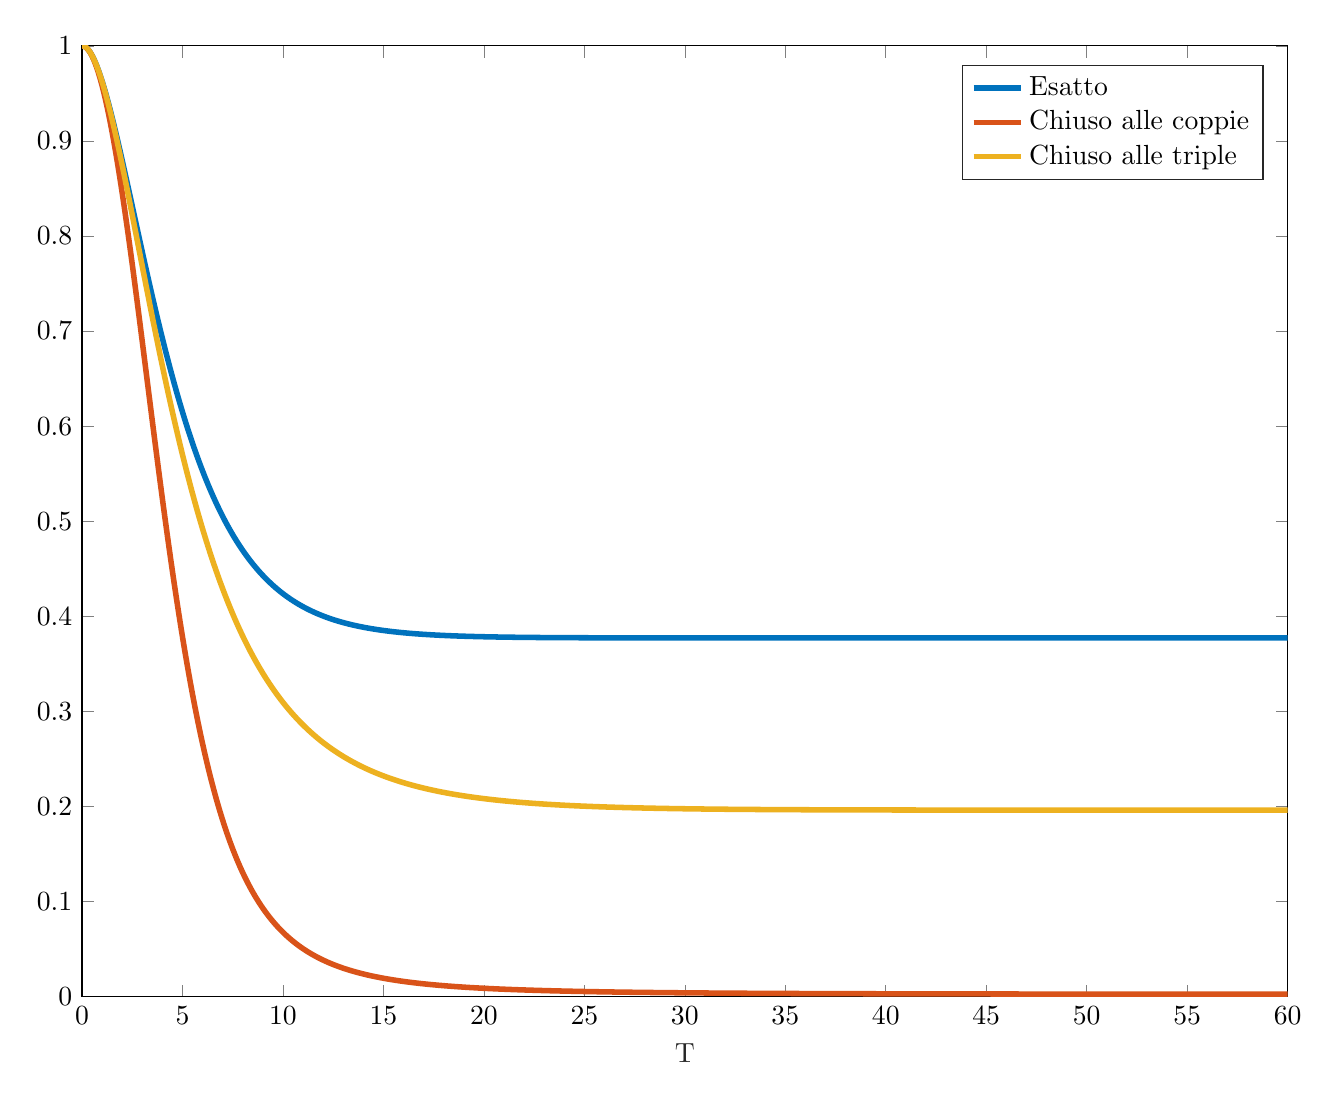
\begin{tikzpicture}

\begin{axis}[%
width=6.028in,
height=4.754in,
at={(1.011in,0.642in)},
scale only axis,
xmin=0,
xmax=60,
xlabel style={font=\color{white!15!black}},
xlabel={T},
ymin=0,
ymax=1,
axis background/.style={fill=white},
legend style={legend cell align=left, align=left, draw=white!15!black}
]
\addplot [color=mycolor1, line width=2.0pt]
  table[row sep=crcr]{%
0	1\\
0.00199053585276749	0.999999821758676\\
0.00398107170553497	0.999999287271421\\
0.00597160755830246	0.999998396893465\\
0.00796214341106994	0.999997150980244\\
0.0123567669950473	0.999993143127503\\
0.0167513905790247	0.999987407889193\\
0.0211460141630021	0.999979949100751\\
0.0255406377469794	0.999970770602233\\
0.0299388563931551	0.999959866624705\\
0.0343370750393307	0.999947247832013\\
0.0387352936855064	0.999932918087308\\
0.043133512331682	0.99991688125802\\
0.0475471725191068	0.999899075937191\\
0.0519608327065316	0.999879559339978\\
0.0563744928939564	0.999858335387465\\
0.0607881530813811	0.999835408004732\\
0.0652173199794049	0.999810691606778\\
0.0696464868774286	0.999784267719513\\
0.0740756537754524	0.999756140321436\\
0.0785048206734761	0.999726313394756\\
0.0829496187548012	0.999694676680182\\
0.0873944168361263	0.999661336466181\\
0.0918392149174515	0.999626296788303\\
0.0962840129987766	0.999589561685518\\
0.100744568101794	0.999550995972635\\
0.105205123204811	0.999510730952902\\
0.109665678307829	0.999468770718551\\
0.114126233410846	0.999425119364942\\
0.118602673075784	0.999379616525619\\
0.123079112740721	0.999332418774366\\
0.127555552405659	0.999283530259728\\
0.132031992070596	0.999232955133084\\
0.136524445545197	0.999180507589601\\
0.141016899019798	0.999126369731132\\
0.1455093524944	0.999070545762162\\
0.150001805969001	0.999013039889722\\
0.154510404254387	0.998953640611314\\
0.159019002539772	0.998892555816567\\
0.163527600825158	0.998829789765537\\
0.168036199110544	0.998765346720531\\
0.172561074936287	0.998698989220849\\
0.17708595076203	0.998630951204912\\
0.181610826587773	0.998561236987975\\
0.186135702413515	0.998489850887247\\
0.190676990405524	0.998416529219182\\
0.195218278397533	0.998341532236025\\
0.199759566389542	0.998264864307858\\
0.204300854381551	0.99818652980642\\
0.208858690959197	0.998106238560546\\
0.213416527536843	0.998024277401581\\
0.217974364114488	0.997940650754059\\
0.222532200692134	0.997855363043875\\
0.227106724202768	0.997768097343535\\
0.231681247713401	0.997679167332637\\
0.236255771224035	0.997588577489792\\
0.240830294734669	0.997496332294675\\
0.245421645441331	0.997402087793233\\
0.250012996147992	0.997306184784038\\
0.254604346854654	0.997208627799406\\
0.259195697561315	0.997109421372416\\
0.263804017673384	0.99700819424998\\
0.268412337785452	0.99690531462263\\
0.273020657897521	0.99680078707601\\
0.27762897800959	0.996694616196225\\
0.282254411746462	0.996586403155648\\
0.286879845483334	0.996476543812783\\
0.291505279220206	0.996365042806223\\
0.296130712957079	0.996251904774722\\
0.300773406613671	0.996136703037344\\
0.305416100270264	0.996019861399835\\
0.310058793926856	0.995901384553362\\
0.314701487583449	0.995781277188947\\
0.319361589521735	0.995659084492062\\
0.324021691460022	0.995535258496532\\
0.328681793398309	0.995409803945715\\
0.333341895336596	0.995282725582526\\
0.338019556071109	0.995153540174664\\
0.342697216805623	0.995022728268747\\
0.347374877540136	0.994890294659947\\
0.35205253827465	0.994756244142687\\
0.356747910447269	0.994620064781757\\
0.361443282619888	0.994482265922303\\
0.366138654792507	0.994342852410934\\
0.370834026965126	0.994201829093197\\
0.375547265516765	0.994058655039184\\
0.380260504068404	0.993913868684887\\
0.384973742620042	0.993767474927966\\
0.389686981171681	0.993619478664712\\
0.394418243246227	0.993469309679876\\
0.399149505320772	0.993317535791578\\
0.403880767395317	0.993164161948147\\
0.408612029469863	0.993009193096236\\
0.41336147459102	0.992852029437397\\
0.418110919712177	0.992693268470303\\
0.422860364833334	0.992532915193569\\
0.427609809954491	0.992370974603824\\
0.432377599961091	0.992206817021958\\
0.437145389967691	0.992041069925322\\
0.44191317997429	0.991873738362433\\
0.44668096998089	0.991704827379509\\
0.451467269141767	0.991533677113809\\
0.456253568302644	0.991360945324967\\
0.461039867463521	0.991186637111017\\
0.465826166624398	0.991010757567379\\
0.47063114173014	0.990832616339664\\
0.475436116835881	0.990652901778434\\
0.480241091941623	0.990471619030852\\
0.485046067047365	0.990288773241155\\
0.489869887370685	0.99010364325504\\
0.494693707694006	0.989916948322967\\
0.499517528017326	0.989728693640843\\
0.504341348340647	0.989538884401329\\
0.509184185682064	0.989346768338733\\
0.51402702302348	0.989153095915621\\
0.518869860364897	0.988957872376255\\
0.523712697706314	0.988761102961329\\
0.528574726619363	0.988562003971675\\
0.533436755532412	0.988361357404694\\
0.53829878444546	0.988159168552612\\
0.543160813358509	0.98795544270377\\
0.548042211039569	0.987749364406118\\
0.55292360872063	0.987541747512065\\
0.55780500640169	0.987332597361411\\
0.56268640408275	0.987121919289747\\
0.56758735048985	0.986908865766242\\
0.572488296896949	0.986694282824967\\
0.577389243304049	0.986478175852903\\
0.582290189711149	0.986260550232503\\
0.587210867601438	0.986040526025034\\
0.592131545491728	0.985818981776135\\
0.597052223382018	0.985595922919578\\
0.601972901272307	0.985371354884277\\
0.606913496388328	0.985144364984483\\
0.611854091504349	0.984915864617257\\
0.61679468662037	0.984685859262764\\
0.621735281736391	0.984454354395988\\
0.626695982628195	0.984220404251613\\
0.631656683519999	0.983984953411577\\
0.636617384411802	0.983748007402045\\
0.641578085303606	0.983509571743672\\
0.646559083672327	0.98326866724142\\
0.651540082041047	0.983026272013021\\
0.656521080409768	0.982782391630246\\
0.661502078778488	0.982537031659021\\
0.666503569383853	0.98228917912712\\
0.671505059989219	0.982039846036422\\
0.676506550594584	0.981789038003902\\
0.68150804119995	0.981536760640362\\
0.686530221876942	0.981281966846773\\
0.691552402553934	0.981025702859716\\
0.696574583230927	0.980767974340972\\
0.701596763907919	0.980508786945815\\
0.706639835866396	0.98024705908213\\
0.711682907824873	0.979983871588318\\
0.71672597978335	0.979719230170567\\
0.721769051741827	0.979453140528221\\
0.72683321952555	0.979184486210138\\
0.731897387309272	0.978914383023414\\
0.736961555092995	0.97864283671824\\
0.742025722876718	0.978369853037629\\
0.747111194287107	0.978094280308223\\
0.752196665697496	0.977817269670045\\
0.757282137107885	0.97753882691689\\
0.762367608518274	0.977258957835032\\
0.767474594900923	0.976976475148993\\
0.772581581283573	0.976692565712589\\
0.777688567666222	0.976407235362809\\
0.782795554048871	0.976120489928786\\
0.78792427039055	0.975831106146045\\
0.793052986732229	0.975540306970049\\
0.798181703073909	0.975248098280582\\
0.803310419415588	0.974954485949224\\
0.808461084325784	0.974658210335209\\
0.81361174923598	0.974360530884015\\
0.818762414146177	0.974061453517812\\
0.823913079056373	0.97376098415022\\
0.82908591482452	0.973457826372435\\
0.834258750592667	0.973153276512815\\
0.839431586360813	0.972847340535507\\
0.84460442212896	0.97254002439576\\
0.849799655005291	0.97222999450725\\
0.854994887881621	0.971918584491747\\
0.860190120757951	0.971605800354966\\
0.865385353634282	0.971291648093377\\
0.870603213699137	0.970974756540108\\
0.875821073763992	0.970656497014573\\
0.881038933828848	0.970336875563643\\
0.886256793893703	0.970015898224591\\
0.891497515445601	0.969692155822238\\
0.896738236997499	0.969367057802491\\
0.901978958549397	0.969040610252967\\
0.907219680101295	0.968712819251329\\
0.912483501408722	0.968382237200377\\
0.917747322716149	0.968050312087533\\
0.923011144023576	0.967717050040742\\
0.928274965331004	0.967382457177642\\
0.933562128954513	0.967045047044285\\
0.938849292578023	0.966706306605565\\
0.944136456201532	0.966366242029344\\
0.949423619825042	0.966024859472814\\
0.954734372782572	0.965680633178794\\
0.960045125740102	0.965335089537381\\
0.965355878697632	0.964988234755934\\
0.970666631655162	0.964640075030783\\
0.976001225418392	0.964289044854154\\
0.981335819181621	0.963936710490052\\
0.98667041294485	0.963583078184914\\
0.99200500670808	0.963228154173783\\
0.997363697280812	0.962870332745004\\
1.00272238785355	0.962511220491182\\
1.00808107842628	0.962150823697415\\
1.01343976899901	0.961789148637038\\
1.0188228172289	0.961424548919564\\
1.02420586545878	0.961058671942506\\
1.02958891368867	0.960691524029197\\
1.03497196191855	0.960323111490839\\
1.04037963341625	0.959951746787766\\
1.04578730491395	0.959579118594248\\
1.05119497641164	0.959205233271429\\
1.05660264790934	0.958830097167953\\
1.06203521338424	0.958451981100932\\
1.06746777885913	0.958072615516885\\
1.07290034433402	0.957692006814344\\
1.07833290980891	0.957310161378968\\
1.08379064506731	0.956925307889959\\
1.08924838032571	0.956539219062339\\
1.09470611558411	0.956151901331599\\
1.10016385084252	0.955763361119982\\
1.1056470369148	0.955371784464716\\
1.11113022298707	0.954978986855011\\
1.11661340905935	0.95458497476289\\
1.12209659513163	0.954189754646746\\
1.12760551858231	0.953791469375167\\
1.13311444203298	0.953391977739819\\
1.13862336548365	0.952991286248824\\
1.14413228893432	0.952589401396296\\
1.14966724184116	0.952184422356571\\
1.15520219474799	0.951778251751113\\
1.16073714765482	0.951370896123712\\
1.16627210056166	0.950962362003764\\
1.17183338076584	0.950550704327301\\
1.17739466097002	0.950137870091388\\
1.18295594117419	0.949723865875048\\
1.18851722137837	0.949308698242523\\
1.19410513262804	0.948890377336704\\
1.19969304387772	0.948470895086909\\
1.20528095512739	0.948050258106961\\
1.21086886637706	0.947628472995503\\
1.21648371859449	0.947203504527376\\
1.22209857081192	0.946777390140901\\
1.22771342302936	0.946350136484262\\
1.23332827524679	0.945921750190066\\
1.23897038457538	0.945490150086655\\
1.24461249390397	0.94505741970176\\
1.25025460323256	0.944623565717482\\
1.25589671256115	0.94418859479995\\
1.26156640151281	0.943750379241692\\
1.26723609046446	0.9433110492512\\
1.27290577941612	0.942870611544051\\
1.27857546836778	0.94242907281945\\
1.28427306633634	0.941984258205439\\
1.28997066430491	0.941538345221924\\
1.29566826227347	0.941091340617517\\
1.30136586024204	0.940643251124048\\
1.30709170327692	0.940191854094465\\
1.31281754631181	0.939739374972921\\
1.31854338934669	0.939285820540611\\
1.32426923238158	0.938831197561545\\
1.33002366371043	0.93837323496267\\
1.33577809503928	0.937914206765464\\
1.34153252636813	0.937454119783261\\
1.34728695769699	0.936992980811795\\
1.35307032782915	0.936528469693615\\
1.35885369796131	0.936062909688224\\
1.36463706809348	0.93559630764064\\
1.37042043822564	0.935128670377867\\
1.37622881553645	0.934657975984608\\
1.38203719284726	0.934186251151717\\
1.38784557015807	0.933713502740253\\
1.39365394746888	0.933239737592897\\
1.39948194569202	0.932763357022515\\
1.40530994391516	0.932285966581078\\
1.41113794213829	0.931807573125033\\
1.41696594036143	0.931328183492157\\
1.4228137248248	0.930846171922117\\
1.42866150928816	0.93036317113504\\
1.43450929375153	0.929879187981882\\
1.44035707821489	0.929394229294635\\
1.44622478964653	0.928906644386903\\
1.45209250107816	0.928418091008538\\
1.45796021250979	0.927928576004031\\
1.46382792394143	0.927438106198621\\
1.46971570462452	0.926945005989889\\
1.4756034853076	0.926450958146903\\
1.48149126599069	0.92595596950672\\
1.48737904667378	0.925460046886862\\
1.49328704060906	0.92496148976845\\
1.49919503454433	0.924462005939698\\
1.50510302847961	0.923961602229264\\
1.51101102241489	0.923460285445991\\
1.51693937480906	0.922956330200663\\
1.52286772720322	0.922451469254184\\
1.52879607959739	0.92194570942585\\
1.53472443199155	0.921439057514862\\
1.540673290528	0.920929763202963\\
1.54662214906446	0.920419584281743\\
1.55257100760091	0.919908527560182\\
1.55851986613736	0.919396599826883\\
1.56448937947106	0.918882025907562\\
1.57045889280476	0.918366588551248\\
1.57642840613847	0.917850294555645\\
1.58239791947216	0.917333150697808\\
1.58838823791446	0.916813356965575\\
1.59437855635675	0.91629272104683\\
1.60036887479904	0.915771249727046\\
1.60635919324133	0.915248949770777\\
1.61237046959671	0.914723996276508\\
1.61838174595208	0.914198221921806\\
1.62439302230746	0.913671633478967\\
1.63040429866284	0.913144237699094\\
1.63643668672632	0.912614184874215\\
1.6424690747898	0.912083332588474\\
1.64850146285328	0.911551687600037\\
1.65453385091676	0.911019256645617\\
1.66058750665404	0.91048416519403\\
1.66664116239132	0.909948295752224\\
1.67269481812859	0.909411655063294\\
1.67874847386587	0.908874249848617\\
1.68482355500326	0.908334180776516\\
1.69089863614064	0.907793355253629\\
1.69697371727803	0.907251780007037\\
1.70304879841541	0.906709461741846\\
1.70914546464501	0.90616447633396\\
1.71524213087462	0.905618756081198\\
1.72133879710422	0.905072307693691\\
1.72743546333383	0.904525137859335\\
1.73355387572031	0.903975297726557\\
1.73967228810678	0.903424744419141\\
1.74579070049326	0.902873484629328\\
1.75190911287974	0.902321525026872\\
1.75804943463327	0.901766892032233\\
1.76418975638681	0.901211567595199\\
1.77033007814035	0.900655558389186\\
1.77647039989388	0.900098871064876\\
1.78263279664118	0.899539507293123\\
1.78879519338848	0.89897947387087\\
1.79495759013578	0.898418777451781\\
1.80111998688309	0.897857424666537\\
1.80730462566597	0.897293392509363\\
1.81348926444885	0.896728712551132\\
1.81967390323173	0.896163391424825\\
1.82585854201462	0.8955974357402\\
1.83206559217232	0.895028797811561\\
1.83827264233002	0.89445953398657\\
1.84447969248772	0.893889650876606\\
1.85068674264543	0.893319155069578\\
1.85691637550678	0.892745974228531\\
1.86314600836813	0.892172189448912\\
1.86937564122948	0.891597807319571\\
1.87560527409083	0.891022834405649\\
1.88185766319929	0.890445173730886\\
1.88811005230775	0.889866931126185\\
1.89436244141622	0.889288113156949\\
1.90061483052468	0.888708726364638\\
1.90689015093446	0.888126649214895\\
1.91316547134424	0.88754401219264\\
1.91944079175402	0.886960821838908\\
1.92571611216381	0.886377084670562\\
1.93201454150218	0.885790654582199\\
1.93831297084055	0.88520368672529\\
1.94461140017892	0.884616187615593\\
1.9509098295173	0.884028163744458\\
1.95723154808653	0.883437444416735\\
1.96355326665576	0.882846209468748\\
1.96987498522499	0.882254465390062\\
1.97619670379422	0.881662218645611\\
1.98254189319299	0.881067274064932\\
1.98888708259176	0.880471836054604\\
1.99523227199053	0.87987591107709\\
2.0015774613893	0.879279505569999\\
2.00794630624256	0.878680399844427\\
2.01431515109582	0.878080822919909\\
2.02068399594908	0.877480781230901\\
2.02705284080234	0.876880281186783\\
2.03344552746868	0.876277078662849\\
2.03983821413503	0.875673427208743\\
2.04623090080137	0.875069333230006\\
2.05262358746771	0.874464803106888\\
2.05904030495676	0.873857568279661\\
2.06545702244581	0.873249906826964\\
2.07187373993486	0.872641825124522\\
2.07829045742391	0.872033329522558\\
2.084731396657	0.871422127101608\\
2.0911723358901	0.870810520393801\\
2.0976132751232	0.870198515744148\\
2.1040542143563	0.869586119471944\\
2.11051956957009	0.868971014244709\\
2.11698492478388	0.868355527100966\\
2.12345027999767	0.86773966435411\\
2.12991563521146	0.867123432291618\\
2.13640560238783	0.866504489268607\\
2.1428955695642	0.86588518672921\\
2.14938553674057	0.865265530954317\\
2.15587550391694	0.864645528198689\\
2.16239028199053	0.864022812495508\\
2.16890506006412	0.863399759703756\\
2.17541983813771	0.86277637607092\\
2.1819346162113	0.86215266781816\\
2.18847440630977	0.861526244724612\\
2.19501419640825	0.860899506996016\\
2.20155398650673	0.86027246084557\\
2.20809377660521	0.859645112459944\\
2.21465878275268	0.859015047369792\\
2.22122378890015	0.858384690121795\\
2.22778879504762	0.857754046893969\\
2.23435380119508	0.857123123837612\\
2.24094422983074	0.856489482291673\\
2.24753465846639	0.855855571086803\\
2.25412508710205	0.85522139636495\\
2.2607155157377	0.854586964241152\\
2.2673315759421	0.853949811902932\\
2.27394763614649	0.853312412424431\\
2.28056369635089	0.852674771910644\\
2.28717975655528	0.852036896439472\\
2.29382166035897	0.851396299062792\\
2.30046356416266	0.850755477082241\\
2.30710546796636	0.850114436564983\\
2.31374737177005	0.849473183550898\\
2.32041533418655	0.848829206974096\\
2.32708329660306	0.848185028345644\\
2.33375125901957	0.84754065369399\\
2.34041922143607	0.846896089020119\\
2.34711345989709	0.846248799218266\\
2.3538076983581	0.845601329930892\\
2.36050193681912	0.84495368714685\\
2.36719617528013	0.844305876827357\\
2.37391691043736	0.843655339832736\\
2.3806376455946	0.843004645930697\\
2.38735838075183	0.842353801069629\\
2.39407911590907	0.841702811170099\\
2.40082657131283	0.841049093101204\\
2.40757402671659	0.840395240713082\\
2.41432148212035	0.839741259912775\\
2.42106893752412	0.839087156579339\\
2.42784333963791	0.838430323637689\\
2.4346177417517	0.837773378973211\\
2.4413921438655	0.837116328450731\\
2.44816654597929	0.836459177906918\\
2.4549681243632	0.835799296357661\\
2.4617697027471	0.835139325688318\\
2.46857128113101	0.834479271720627\\
2.47537285951492	0.833819140248002\\
2.48220184698832	0.833156276402645\\
2.48903083446173	0.832493346044435\\
2.49585982193513	0.831830354951152\\
2.50268880940853	0.831167308872091\\
2.50954544177924	0.830501529113496\\
2.51640207414995	0.829835705451944\\
2.52325870652066	0.829169843620389\\
2.53011533889137	0.828503949323143\\
2.53699985562036	0.827835320039893\\
2.54388437234935	0.827166669464428\\
2.55076888907833	0.826498003284008\\
2.55765340580732	0.825829327157098\\
2.5645660494942	0.825157914792538\\
2.57147869318108	0.824486503745555\\
2.57839133686796	0.823815099656852\\
2.58530398055484	0.823143708138183\\
2.59224499685821	0.822469579197461\\
2.59918601316159	0.821795474181377\\
2.60612702946496	0.821121398683211\\
2.61306804576833	0.820447358267151\\
2.62003768421203	0.819770579238379\\
2.62700732265572	0.819093846736811\\
2.63397696109942	0.818417166307444\\
2.64094659954311	0.817740543466038\\
2.64794511298781	0.817061180871296\\
2.65494362643251	0.816381887400082\\
2.6619421398772	0.815702668548248\\
2.6689406533219	0.815023529782269\\
2.67596829852112	0.814341650123513\\
2.68299594372033	0.813659862176647\\
2.69002358891955	0.812978171387516\\
2.69705123411877	0.812296583172455\\
2.70410827073433	0.811612253027156\\
2.71116530734989	0.810928037172412\\
2.71822234396545	0.810243941003205\\
2.72527938058101	0.809559969884872\\
2.73236607296869	0.808873255733056\\
2.73945276535637	0.8081866784391\\
2.74653945774405	0.807500243346265\\
2.75362615013173	0.806813955768036\\
2.76074276611797	0.80612492411157\\
2.76785938210422	0.805436051867224\\
2.77497599809046	0.804747344325684\\
2.78209261407671	0.80405880674773\\
2.78923942490227	0.803367524116398\\
2.79638623572783	0.802676423436726\\
2.80353304655339	0.801985509945964\\
2.81067985737896	0.801294788851337\\
2.81785713902212	0.800601321675728\\
2.82503442066529	0.799908058974995\\
2.83221170230846	0.799215005932098\\
2.83938898395163	0.798522167699853\\
2.84659701614953	0.797826582407408\\
2.85380504834743	0.797131224095098\\
2.86101308054533	0.796436097890741\\
2.86822111274323	0.795741208891892\\
2.87546017926332	0.795043571882027\\
2.88269924578341	0.794346184337994\\
2.88993831230351	0.793649051331612\\
2.8971773788236	0.792952177904329\\
2.90444776780364	0.792252555517335\\
2.91171815678368	0.791553205060737\\
2.91898854576373	0.790854131549502\\
2.92625893474377	0.79015533996812\\
2.93356093845992	0.789453798509476\\
2.94086294217606	0.788752551423082\\
2.94816494589221	0.788051603666203\\
2.95546694960836	0.78735096016552\\
2.96280086487659	0.786647565869443\\
2.97013478014483	0.785944488363232\\
2.97746869541306	0.785241732545591\\
2.9848026106813	0.784539303284548\\
2.99216873909201	0.783834122294099\\
2.99953486750271	0.783129280485392\\
3.00690099591342	0.782424782697724\\
3.01426712432413	0.781720633739616\\
3.02166577186631	0.781013732145562\\
3.02906441940849	0.780307192097875\\
3.03646306695067	0.77960101837559\\
3.04386171449286	0.778895215726875\\
3.05129319192691	0.778186659534979\\
3.05872466936097	0.77747848722535\\
3.06615614679503	0.776770703515908\\
3.07358762422909	0.77606331309362\\
3.08105224696524	0.775353168239552\\
3.0885168697014	0.774643429573451\\
3.09598149243755	0.773934101751273\\
3.1034461151737	0.773225189397932\\
3.11094420406679	0.772513521675254\\
3.11844229295988	0.771802282414669\\
3.12594038185297	0.771091476209312\\
3.13343847074605	0.770381107621199\\
3.14097035080817	0.769667982807694\\
3.14850223087028	0.768955308697318\\
3.1560341109324	0.768243089819536\\
3.16356599099451	0.767531330672614\\
3.17113199342146	0.766816814342122\\
3.17869799584842	0.766102770921441\\
3.18626399827537	0.765389204875508\\
3.19383000070233	0.764676120637992\\
3.20143046110215	0.763960278332976\\
3.20903092150198	0.763244931108624\\
3.21663138190181	0.762530083364495\\
3.22423184230164	0.761815739468807\\
3.2318671021242	0.761098636569872\\
3.23950236194676	0.76038205088534\\
3.24713762176933	0.759665986748535\\
3.25477288159189	0.758950448461375\\
3.26244328804483	0.758232150200888\\
3.27011369449776	0.757514391250146\\
3.2777841009507	0.756797175875381\\
3.28545450740363	0.75608050831136\\
3.29316041266953	0.75536107985237\\
3.30086631793543	0.754642212758681\\
3.30857222320133	0.753923911228576\\
3.31627812846722	0.753206179428818\\
3.32401989110489	0.752485685739595\\
3.33176165374256	0.751765775430258\\
3.33950341638023	0.751046452630283\\
3.3472451790179	0.750327721437575\\
3.35502316313618	0.749606227375318\\
3.36280114725446	0.748885338665266\\
3.37057913137275	0.748165059367225\\
3.37835711549103	0.747445393509386\\
3.38617169154667	0.746722963752538\\
3.3939862676023	0.746001161276769\\
3.40180084365794	0.745279990071358\\
3.40961541971357	0.744559454093924\\
3.41746696420648	0.743836153177668\\
3.42531850869938	0.743113501426706\\
3.43317005319229	0.742391502758927\\
3.4410215976852	0.741670161060521\\
3.44891049346576	0.740946053355703\\
3.45679938924632	0.740222616654573\\
3.46468828502688	0.739499854802762\\
3.47257718080744	0.73877777161417\\
3.48050381756295	0.738052921290614\\
3.48843045431847	0.737328763762236\\
3.49635709107398	0.736605302801542\\
3.50428372782949	0.73588254214928\\
3.51224850159594	0.735157013229016\\
3.52021327536239	0.734432198847353\\
3.52817804912884	0.733708102702804\\
3.53614282289529	0.732984728462101\\
3.54414613607264	0.732258584826045\\
3.55214944924998	0.731533177422781\\
3.56015276242733	0.730808509875957\\
3.56815607560468	0.730084585777418\\
3.57619833889781	0.729357890998277\\
3.58424060219095	0.728631954096074\\
3.59228286548408	0.727906778618717\\
3.60032512877721	0.727182368082297\\
3.60840675922679	0.726455185613617\\
3.61648838967638	0.725728782614804\\
3.62457002012596	0.72500316255715\\
3.63265165057554	0.724278328880116\\
3.64077307248204	0.723550721981961\\
3.64889449438855	0.722823916094374\\
3.65701591629505	0.722097914611151\\
3.66513733820155	0.721372720894247\\
3.67329898353354	0.720644752607071\\
3.68146062886554	0.719917606818002\\
3.68962227419754	0.719191286842452\\
3.69778391952953	0.718465795963995\\
3.70598622860803	0.717737529059123\\
3.71418853768653	0.717010106085933\\
3.72239084676502	0.716283530280568\\
3.73059315584352	0.715557804847335\\
3.73883657626523	0.714829301934817\\
3.74707999668693	0.714101664332568\\
3.75532341710863	0.71337489519657\\
3.76356683753034	0.712648997650976\\
3.77185182516863	0.711920321102255\\
3.78013681280692	0.711192531186569\\
3.78842180044522	0.710465630978843\\
3.79670678808351	0.709739623522185\\
3.80503380745825	0.709010835450583\\
3.81336082683299	0.708282955278201\\
3.82168784620774	0.707555985998004\\
3.83001486558248	0.70682993057116\\
3.83838438958511	0.706101092869558\\
3.84675391358775	0.705373184275945\\
3.85512343759039	0.704646207700424\\
3.86349296159302	0.703920166021322\\
3.8719054722877	0.703191340306052\\
3.88031798298237	0.702463464849459\\
3.88873049367705	0.701736542477872\\
3.89714300437172	0.701010575985873\\
3.90559899284027	0.700281823625211\\
3.91405498130882	0.699554042615114\\
3.92251096977737	0.698827235697222\\
3.93096695824593	0.698101405581464\\
3.93946692479213	0.697372787693018\\
3.94796689133833	0.696645162187539\\
3.95646685788454	0.695918531721059\\
3.96496682443074	0.695192898917933\\
3.97351127881372	0.694464476364191\\
3.98205573319669	0.693737067165678\\
3.99060018757967	0.693010673891889\\
3.99914464196265	0.692285299080687\\
4.00773410425464	0.691557132412381\\
4.01632356654662	0.690830000010957\\
4.02491302883861	0.690103904358436\\
4.0335024911306	0.689378847905262\\
4.04213749081375	0.688650997455598\\
4.05077249049689	0.687924202123145\\
4.05940749018004	0.687198464301517\\
4.06804248986318	0.686473786352797\\
4.07672356764034	0.685746312101832\\
4.08540464541749	0.685019913756793\\
4.09408572319465	0.684294593621931\\
4.10276680097181	0.683570353970033\\
4.11149450824228	0.682843315608809\\
4.12022221551276	0.682117373880159\\
4.12894992278323	0.681392530998021\\
4.1376776300537	0.680668789144934\\
4.14645252883691	0.679942246101057\\
4.15522742762012	0.67921682035384\\
4.16400232640333	0.678492514025946\\
4.17277722518654	0.677769329208709\\
4.18159988926615	0.677043340571352\\
4.19042255334575	0.676318489831943\\
4.19924521742536	0.675594779020892\\
4.20806788150496	0.674872210137363\\
4.21693889629988	0.674146834689816\\
4.22580991109479	0.673422617678393\\
4.23468092588971	0.672699561040279\\
4.24355194068463	0.671977666681489\\
4.2524719033702	0.671252962913006\\
4.26139186605577	0.670529438055408\\
4.27031182874135	0.669807093951656\\
4.27923179142692	0.669085932413638\\
4.28820131218307	0.668361958440768\\
4.29717083293922	0.667639183790098\\
4.30614035369538	0.66691761020937\\
4.31510987445153	0.666197239415347\\
4.32412957614907	0.665474053032334\\
4.33314927784661	0.664752086319247\\
4.34216897954416	0.664031340927597\\
4.3511886812417	0.663311818478019\\
4.36025919971018	0.662589477159914\\
4.36932971817866	0.66186837579575\\
4.37840023664715	0.661148515939786\\
4.38747075511563	0.660429899115513\\
4.39659274002011	0.659708459973978\\
4.40571472492458	0.658988281006755\\
4.41483670982906	0.658269363669818\\
4.42395869473353	0.657551709388486\\
4.43313280988389	0.656831229174936\\
4.44230692503424	0.656112029292527\\
4.45148104018459	0.655394111097902\\
4.46065515533495	0.65467747591717\\
4.469882079136	0.653958011015916\\
4.47910900293706	0.653239846539261\\
4.48833592673811	0.652522983743459\\
4.49756285053916	0.651807423854356\\
4.50684327607396	0.651089030305535\\
4.51612370160877	0.650371957211537\\
4.52540412714357	0.649656205727151\\
4.53468455267837	0.648941776976898\\
4.54401918924822	0.648224510387736\\
4.55335382581807	0.647508584220893\\
4.56268846238792	0.64679399952861\\
4.57202309895777	0.646080757333\\
4.58141267108196	0.645364672987779\\
4.59080224320616	0.644649948969802\\
4.60019181533036	0.64393658622766\\
4.60958138745456	0.643224585679965\\
4.61902663678989	0.64250973842562\\
4.62847188612523	0.641796271341509\\
4.63791713546056	0.641084185271456\\
4.6473623847959	0.640373481029459\\
4.65686406984621	0.639659925333481\\
4.66636575489653	0.63894776958927\\
4.67586743994685	0.638237014534747\\
4.68536912499717	0.63752766087817\\
4.69492802222378	0.636815450781042\\
4.7044869194504	0.636104660356477\\
4.71404581667701	0.63539529023534\\
4.72360471390363	0.634687341019005\\
4.73320764525141	0.633977561870957\\
4.74281057659919	0.633269217875996\\
4.75241350794698	0.632562309554549\\
4.76201643929476	0.631856837397901\\
4.77165794452804	0.631149976734965\\
4.78129944976131	0.630444564701867\\
4.79094095499459	0.629740601707782\\
4.80058246022786	0.629038088133163\\
4.81026314694842	0.628334178280334\\
4.81994383366897	0.627631730332827\\
4.82962452038952	0.626930744588973\\
4.83930520711008	0.62623122131881\\
4.84902565638322	0.62553029655961\\
4.85874610565637	0.624830846772498\\
4.86846655492951	0.624132872145348\\
4.87818700420266	0.623436372838168\\
4.88794780523678	0.622738466858853\\
4.89770860627089	0.622042048712455\\
4.90746940730501	0.621347118476764\\
4.91723020833913	0.620653676202129\\
4.92703195872998	0.61995882209936\\
4.93683370912084	0.61926546848714\\
4.9466354595117	0.618573615333522\\
4.95643720990256	0.617883262579554\\
4.96628051524823	0.617191492912535\\
4.97612382059389	0.616501236192984\\
4.98596712593956	0.615812492279559\\
4.99581043128522	0.615125261004338\\
5.00569590732134	0.614436607669498\\
5.01558138335745	0.613749479541357\\
5.02546685939356	0.613063876369493\\
5.03535233542967	0.612379797877338\\
5.04528060635073	0.611694292253313\\
5.05520887727179	0.611010323899909\\
5.06513714819285	0.610327892457923\\
5.07506541911391	0.609646997542444\\
5.08503711889176	0.608964670423353\\
5.0950088186696	0.60828389244615\\
5.10498051844744	0.607604663143138\\
5.11495221822528	0.606926982021347\\
5.12496799094167	0.606247863621065\\
5.13498376365806	0.605570306043919\\
5.14499953637444	0.604894308713983\\
5.15501530909083	0.604219871030501\\
5.16507580953502	0.603543990969745\\
5.17513630997921	0.602869683226047\\
5.18519681042339	0.602196947115499\\
5.19525731086758	0.601525781929807\\
5.2053632039849	0.600853169301178\\
5.21546909710223	0.600182140298586\\
5.22557499021955	0.599512694130377\\
5.23568088333688	0.598844829980956\\
5.24583284576096	0.598175513274013\\
5.25598480818505	0.597507791319883\\
5.26613677060914	0.596841663219378\\
5.27628873303322	0.596177128049819\\
5.28648745229033	0.595511135233062\\
5.29668617154743	0.594846748116043\\
5.30688489080453	0.594183965692236\\
5.31708361006163	0.593522786932075\\
5.32732978639303	0.592860145362116\\
5.33757596272443	0.592199120261753\\
5.34782213905582	0.591539710517307\\
5.35806831538722	0.590881914992505\\
5.36836266133408	0.590222651472515\\
5.37865700728095	0.58956501501744\\
5.38895135322782	0.588909004406602\\
5.39924569917468	0.588254618397192\\
5.40958894010065	0.587598759173677\\
5.41993218102661	0.586944537438397\\
5.43027542195257	0.586291951863823\\
5.44061866287853	0.585641001100749\\
5.45101153706255	0.584988571888487\\
5.46140441124658	0.584337790418214\\
5.4717972854306	0.583688655255672\\
5.48219015961463	0.583041164945389\\
5.49263341945276	0.582392190883131\\
5.50307667929089	0.581744874649714\\
5.51351993912902	0.581099214704257\\
5.52396319896715	0.580455209485132\\
5.53445761187213	0.579809715113641\\
5.54495202477712	0.579165888493741\\
5.5554464376821	0.578523727978016\\
5.56594085058709	0.57788323189877\\
5.57648719831941	0.577241241236843\\
5.58703354605173	0.576600928087592\\
5.59757989378405	0.57596229069713\\
5.60812624151637	0.575325327291767\\
5.61872532103302	0.574686863817564\\
5.62932440054967	0.574050087458003\\
5.63992348006633	0.573414996352777\\
5.65052255958298	0.572781588622248\\
5.66117518401188	0.572146675249526\\
5.67182780844078	0.571513458436991\\
5.68248043286967	0.570881936217939\\
5.69313305729857	0.57025210660682\\
5.70384005671797	0.569620765675478\\
5.71454705613736	0.568991130596223\\
5.72525405555675	0.568363199295964\\
5.73596105497615	0.567736969683245\\
5.74672327665992	0.567109222983043\\
5.75748549834369	0.566483191275873\\
5.76824772002746	0.565858872382238\\
5.77900994171123	0.565236264104768\\
5.78982825023888	0.56461213290684\\
5.80064655876654	0.563989725694474\\
5.81146486729419	0.563369040181737\\
5.82228317582184	0.56275007406531\\
5.83315845473553	0.562129579064966\\
5.84403373364921	0.561510816897198\\
5.8549090125629	0.560893785169574\\
5.86578429147658	0.560278481472775\\
5.87671744355088	0.559661642815785\\
5.88765059562518	0.559046545695661\\
5.89858374769948	0.558433187613387\\
5.90951689977378	0.557821566053567\\
5.92050884813521	0.557208403315094\\
5.93150079649664	0.556596990678004\\
5.94249274485807	0.555987325536595\\
5.9534846932195	0.555379405269292\\
5.96453638108293	0.554769937512167\\
5.97558806894636	0.554162228283844\\
5.98663975680979	0.553556274871806\\
5.99769144467322	0.55295207454817\\
6.00880383710542	0.552346320268695\\
6.01991622953761	0.551742332811372\\
6.0310286219698	0.551140109356709\\
6.042141014402	0.550539647070371\\
6.05331509935885	0.549937624188749\\
6.0644891843157	0.549337376291699\\
6.07566326927256	0.548738900452576\\
6.08683735422941	0.548142193730413\\
6.09807414230094	0.547543919652601\\
6.10931093037248	0.546947428593692\\
6.12054771844401	0.54635271751968\\
6.13178450651555	0.545759783382765\\
6.14308503319571	0.54516527492746\\
6.15438555987588	0.544572557400632\\
6.16568608655605	0.543981627660675\\
6.17698661323621	0.543392482552726\\
6.18835193888863	0.542801756005233\\
6.19971726454106	0.542212828174111\\
6.21108259019348	0.54162569580989\\
6.2224479158459	0.541040355650384\\
6.23387912710053	0.540453426741613\\
6.24531033835517	0.539868304218699\\
6.2567415496098	0.539284984724016\\
6.26817276086443	0.538703464887764\\
6.2796709718506	0.538120348785365\\
6.29116918283678	0.537539046623309\\
6.30266739382295	0.536959554935483\\
6.31416560480912	0.536381870244157\\
6.32573195844141	0.535802581544184\\
6.33729831207371	0.535225114227577\\
6.34886466570601	0.534649464719378\\
6.36043101933831	0.53407562943357\\
6.37206668825559	0.533500182172552\\
6.38370235717287	0.532926563630014\\
6.39533802609016	0.532354770121757\\
6.40697369500744	0.531784797953094\\
6.41867988207414	0.53121320564334\\
6.43038606914084	0.530643449282688\\
6.44209225620754	0.530075525077271\\
6.45379844327423	0.529509429223309\\
6.46557638449348	0.528941704772323\\
6.47735432571273	0.528375823400596\\
6.48913226693197	0.527811781204128\\
6.50091020815122	0.527249574269585\\
6.51276117329228	0.526685730017193\\
6.52461213843333	0.526123735877655\\
6.53646310357439	0.525563587836327\\
6.54831406871544	0.52500528186983\\
6.56023936237899	0.524445329605241\\
6.57216465604253	0.523887234394432\\
6.58408994970607	0.523330992111578\\
6.59601524336962	0.52277659862271\\
6.608016207688	0.522220549527953\\
6.62001717200638	0.521666364339628\\
6.63201813632476	0.521114038820136\\
6.64401910064313	0.520563568724343\\
6.65609711612489	0.520011433410394\\
6.66817513160664	0.519461168771536\\
6.68025314708839	0.518912770457762\\
6.69233116257014	0.51836623411215\\
6.70448764976455	0.517818022619091\\
6.71664413695897	0.517271688490202\\
6.72880062415338	0.51672722726239\\
6.7409571113478	0.516184634466269\\
6.75319353351478	0.515640356222703\\
6.76542995568177	0.51509796195764\\
6.77766637784875	0.514557447094169\\
6.78990280001574	0.514018807049725\\
6.80222066442117	0.513478470899837\\
6.8145385288266	0.512940025272847\\
6.82685639323203	0.512403465477243\\
6.83917425763746	0.511868786816509\\
6.85157511856051	0.511332400975453\\
6.86397597948357	0.510797912137034\\
6.87637684040662	0.510265315494301\\
6.88877770132968	0.509734606235961\\
6.90126316148383	0.509202178321148\\
6.91374862163799	0.508671653829299\\
6.92623408179214	0.508143027837133\\
6.93871954194629	0.507616295417692\\
6.95129125486549	0.507087832441967\\
6.96386296778468	0.506561279255604\\
6.97643468070388	0.506036630818031\\
6.98900639362307	0.505513882085683\\
7.00166606764739	0.504989390390111\\
7.0143257416717	0.504466814802535\\
7.02698541569601	0.503946150164072\\
7.03964508972033	0.503427391313538\\
7.05239448925109	0.502906876622812\\
7.06514388878186	0.502388284316947\\
7.07789328831262	0.501871609117657\\
7.09064268784339	0.501356845745063\\
7.10348363709426	0.500840313123935\\
7.11632458634514	0.500325709129307\\
7.12916553559601	0.499813028362327\\
7.14200648484689	0.499302265423267\\
7.15494087138423	0.498789719251357\\
7.16787525792157	0.49827910791935\\
7.18080964445891	0.497770425906585\\
7.19374403099625	0.497263667692257\\
7.20677380774895	0.496755111707496\\
7.21980358450165	0.496248496754745\\
7.23283336125435	0.495743817190207\\
7.24586313800706	0.495241067370692\\
7.25899032889946	0.494736504577063\\
7.27211751979186	0.494233888994181\\
7.28524471068426	0.493733214853699\\
7.29837190157667	0.493234476388647\\
7.31159860422458	0.492733909090775\\
7.32482530687249	0.492235295177011\\
7.3380520095204	0.491738628752949\\
7.35127871216831	0.491243903926344\\
7.36460710304072	0.490747333677556\\
7.37793549391314	0.490252722989598\\
7.39126388478556	0.489760065840395\\
7.40459227565797	0.489269356210835\\
7.41802461355885	0.488776783836251\\
7.43145695145972	0.488286177211512\\
7.4448892893606	0.487797530185159\\
7.45832162726148	0.487310836609515\\
7.47186025959003	0.486822262136339\\
7.48539889191859	0.486335659624204\\
7.49893752424715	0.485851022790435\\
7.51247615657571	0.485368345356975\\
7.52612352432791	0.484883768006016\\
7.53977089208011	0.484401168859878\\
7.55341825983232	0.483920541502713\\
7.56706562758452	0.483441879524145\\
7.58082427117841	0.482961297684382\\
7.5945829147723	0.482482700336894\\
7.60834155836619	0.482006080930566\\
7.62210020196009	0.481531432920639\\
7.63597276754062	0.481054844121519\\
7.64984533312116	0.48058024615764\\
7.66371789870169	0.480107632340386\\
7.67759046428223	0.479636995988402\\
7.69157971106386	0.479164396852477\\
7.70556895784549	0.478693794963073\\
7.71955820462712	0.478225183491682\\
7.73354745140875	0.477758555617988\\
7.7476562591015	0.477289941829104\\
7.76176506679424	0.476823331780029\\
7.77587387448699	0.476358718499807\\
7.78998268217974	0.475896095026628\\
7.80421406003167	0.475431461263443\\
7.81844543788359	0.474968837830312\\
7.83267681573552	0.474508217611091\\
7.84690819358745	0.47404959349976\\
7.86126528820976	0.473588933431042\\
7.87562238283208	0.473130290395324\\
7.8899794774544	0.472673657128333\\
7.90433657207672	0.472219026376937\\
7.91882267896367	0.471762332558598\\
7.93330878585062	0.471307662606364\\
7.94779489273757	0.470855009104685\\
7.96228099962452	0.470404364650191\\
7.97689957365268	0.469951628483443\\
7.99151814768085	0.46950092316482\\
8.00613672170902	0.469052241124105\\
8.02075529573718	0.46860557480434\\
8.03550996276884	0.468156786485598\\
8.0502646298005	0.46771003616612\\
8.06501929683216	0.467265316117382\\
8.07977396386382	0.466822618625231\\
8.09466853533245	0.466377767035128\\
8.10956310680107	0.465934960786869\\
8.12445767826969	0.465494191989703\\
8.13935224973832	0.465055452768402\\
8.15439073744049	0.464614525391506\\
8.16942922514267	0.464175650914786\\
8.18446771284484	0.463738821281037\\
8.19950620054702	0.463304028449767\\
8.2146928332504	0.46286701127836\\
8.22987946595378	0.462432054807803\\
8.24506609865717	0.461999150809868\\
8.26025273136055	0.461568291074278\\
8.27559197362809	0.461135168490501\\
8.29093121589562	0.460704114679833\\
8.30627045816316	0.460275121238087\\
8.32160970043069	0.45984817978031\\
8.33710627308224	0.459418934439574\\
8.35260284573378	0.458991766247885\\
8.36809941838533	0.458566666619748\\
8.38359599103687	0.458143626990239\\
8.39925489573158	0.457718239643119\\
8.41491380042629	0.457294938160428\\
8.430572705121	0.456873713769555\\
8.44623160981571	0.456454557719853\\
8.46205815432056	0.45603300707726\\
8.4778846988254	0.455613551393215\\
8.49371124333024	0.455196181701677\\
8.50953778783509	0.45478088906002\\
8.52553761739547	0.454363151561061\\
8.54153744695585	0.453947518537597\\
8.55753727651623	0.453533980823271\\
8.57353710607661	0.453122529276662\\
8.58971623619016	0.452708578899319\\
8.60589536630372	0.452296742986082\\
8.62207449641727	0.451887012162765\\
8.63825362653082	0.451479377081701\\
8.65461848330403	0.451069185044318\\
8.67098334007723	0.450661117986446\\
8.68734819685043	0.45025516631783\\
8.70371305362364	0.449851320476401\\
8.72018188980809	0.449447024964282\\
8.73665072599255	0.44904484278108\\
8.75311956217701	0.44864476426797\\
8.76958839836146	0.448246779795427\\
8.78614348346302	0.44784881186571\\
8.80269856856458	0.447452940544318\\
8.81925365366614	0.447059156139355\\
8.83580873876771	0.446667448989204\\
8.85245111606455	0.446275760421291\\
8.86909349336139	0.445886151585106\\
8.88573587065824	0.445498612758064\\
8.90237824795508	0.445113134248816\\
8.91910883699713	0.44472767951133\\
8.93583942603918	0.444344287445115\\
8.95257001508123	0.443962948299487\\
8.96930060412328	0.443583652355937\\
8.98612034063892	0.443204385147709\\
9.00294007715455	0.442827163374544\\
9.01975981367019	0.442451977260208\\
9.03657955018582	0.442078817061574\\
9.05348938408815	0.441705690392902\\
9.07039921799048	0.441334591754774\\
9.08730905189281	0.440965511347931\\
9.10421888579513	0.440598439407135\\
9.12121978296026	0.440231405592988\\
9.13822068012539	0.439866382244268\\
9.15522157729052	0.43950335954118\\
9.17222247445565	0.439142327698849\\
9.18931541587169	0.43878133841151\\
9.20640835728774	0.438422341871222\\
9.22350129870378	0.438065328240113\\
9.24059424011982	0.437710287716112\\
9.25778022278737	0.437355293998296\\
9.27496620545493	0.437002275163282\\
9.29215218812249	0.436651221357545\\
9.30933817079004	0.436302122764234\\
9.32661820779546	0.435953075060338\\
9.34389824480088	0.435605984236357\\
9.3611782818063	0.435260840425508\\
9.37845831881172	0.434917633798537\\
9.39583344002363	0.434574481972762\\
9.41320856123555	0.434233268892603\\
9.43058368244747	0.433893984680378\\
9.44795880365938	0.433556619496775\\
9.46543005570071	0.433219312866007\\
9.48290130774205	0.432883926722187\\
9.50037255978338	0.432550451179066\\
9.51784381182471	0.432218876389586\\
9.53541225878365	0.431887363741213\\
9.55298070574258	0.431557753203786\\
9.57054915270152	0.431230034884782\\
9.58811759966045	0.430904198931681\\
9.60578432346384	0.430578428548395\\
9.62345104726722	0.430254541789656\\
9.64111777107061	0.42993252875893\\
9.658784494874	0.429612379600483\\
9.67655059520445	0.429292299293127\\
9.6943166955349	0.428974084020265\\
9.71208279586536	0.428657723883586\\
9.72984889619581	0.428343209026357\\
9.74771549159443	0.428028766144647\\
9.76558208699305	0.42771616961053\\
9.78344868239167	0.427405409526114\\
9.80131527779029	0.427096476035851\\
9.81928350543996	0.42678761750335\\
9.83725173308963	0.42648058654127\\
9.8552199607393	0.426175373254306\\
9.87318818838897	0.425871967790243\\
9.89125920482513	0.425568640122133\\
9.90933022126129	0.425267121163552\\
9.92740123769745	0.424967401023912\\
9.94547225413361	0.424669469856452\\
9.96364723590061	0.424371619178791\\
9.9818222176676	0.424075558272545\\
9.99999719943459	0.423781277253942\\
10.0181721812016	0.423488766283762\\
10.0364523247657	0.423196338364987\\
10.0547324683298	0.42290568120859\\
10.0730126118939	0.422616784939686\\
10.0912927554579	0.422329639728648\\
10.1096792783833	0.42204257999005\\
10.1280658013086	0.421757271940222\\
10.146452324234	0.421473705715199\\
10.1648388471593	0.421191871496966\\
10.1833329877765	0.420910125047594\\
10.2018271283938	0.420630111154911\\
10.220321269011	0.420351819967876\\
10.2388154096282	0.420075241682075\\
10.257418428294	0.419798753328117\\
10.2760214469598	0.419523978346452\\
10.2946244656257	0.41925090690093\\
10.3132274842915	0.418979529202696\\
10.3319406634311	0.418708243476067\\
10.3506538425707	0.418438651890992\\
10.3693670217104	0.418170744628154\\
10.38808020085	0.417904511916175\\
10.4069048454226	0.417638373096007\\
10.4257294899953	0.41737390914619\\
10.4445541345679	0.417111110266143\\
10.4633787791406	0.416849966703859\\
10.4823162175897	0.416588918831123\\
10.5012536560388	0.416329526522929\\
10.5201910944879	0.416071779999304\\
10.539128532937	0.41581566952947\\
10.5581801172831	0.41555965643386\\
10.5772317016292	0.415305279568061\\
10.5962832859753	0.41505252917455\\
10.6153348703214	0.414801395545604\\
10.6345019773376	0.414550360857229\\
10.6536690843538	0.41430094304071\\
10.67283619137	0.414053132362785\\
10.6920032983861	0.413806919140579\\
10.7112873293394	0.413560806321037\\
10.7305713602926	0.413316290997639\\
10.7498553912458	0.413073363463157\\
10.769139422199	0.412832014061328\\
10.7885418041401	0.412590766413804\\
10.8079441860811	0.412351096874442\\
10.8273465680222	0.412112995763793\\
10.8467489499633	0.411876453453938\\
10.8662711360792	0.411640014145893\\
10.8857933221952	0.411405133551112\\
10.9053155083112	0.411171802019638\\
10.9248376944271	0.410940009953592\\
10.9444811647161	0.410708322035046\\
10.9641246350051	0.410478173433216\\
10.9837681052941	0.410249554529321\\
11.0034115755831	0.410022455757188\\
11.02317783773	0.40979546217668\\
11.0429440998769	0.409569988519906\\
11.0627103620238	0.409346025200906\\
11.0824766241707	0.40912356268685\\
11.102367213876	0.408901206313811\\
11.1222578035813	0.408680350480152\\
11.1421483932866	0.408460985634354\\
11.1620389829919	0.408243102278532\\
11.182055464688	0.408025325920726\\
11.202071946384	0.407809030731555\\
11.22208842808	0.407594207195527\\
11.2421049097761	0.407380845851276\\
11.2622488777205	0.407167592268224\\
11.282392845665	0.406955800501617\\
11.3025368136094	0.406745461073543\\
11.3226807815539	0.4065365645607\\
11.3429428732039	0.406327889246286\\
11.363204964854	0.406120654861513\\
11.3834670565041	0.405914851982869\\
11.4037291481542	0.405710471241795\\
11.4240073959591	0.405507342047656\\
11.444285643764	0.405305618650589\\
11.464563891569	0.405105291824253\\
11.4848421393739	0.404906352396477\\
11.5051410232308	0.404708590901095\\
11.5254399070878	0.404512201401366\\
11.5457387909448	0.404317174859512\\
11.5660376748017	0.404123502291187\\
11.5863613245615	0.403930940931769\\
11.6066849743212	0.403739718989014\\
11.627008624081	0.40354982760595\\
11.6473322738407	0.403361257978333\\
11.6676846007299	0.403173738054805\\
11.6880369276191	0.402987526107496\\
11.7083892545083	0.402802613453108\\
11.7287415813975	0.402618991460392\\
11.7491263024508	0.402436362342761\\
11.7695110235041	0.402255010824216\\
11.7898957445574	0.402074928388555\\
11.8102804656107	0.401896106570971\\
11.8307011258767	0.401718224995378\\
11.8511217861426	0.401541591637438\\
11.8715424464086	0.401366198141955\\
11.8919631066745	0.401192036204507\\
11.9124230970895	0.401018765666981\\
11.9328830875046	0.400846714900208\\
11.9533430779196	0.400675875704354\\
11.9738030683347	0.400506239929763\\
11.9943056417768	0.400337450145565\\
12.014808215219	0.400169852564285\\
12.0353107886612	0.400003439136209\\
12.0558133621033	0.399838201861216\\
12.0763616495731	0.399673768267777\\
12.0969099370428	0.399510500138266\\
12.1174582245125	0.399348389568196\\
12.1380065119823	0.399187428702115\\
12.1586035338403	0.399027232041977\\
12.1792005556983	0.39886817488966\\
12.1997975775563	0.398710249481337\\
12.2203945994143	0.398553448101678\\
12.2410432774846	0.398397374031243\\
12.2616919555548	0.398242414253466\\
12.2823406336251	0.398088561140909\\
12.3029893116954	0.39793580711411\\
12.3236924799435	0.397783745854088\\
12.3443956481917	0.397632774374125\\
12.3650988164398	0.397482885179164\\
12.385801984688	0.397334070821618\\
12.406562398648	0.397185916843772\\
12.4273228126081	0.397038828800713\\
12.4480832265682	0.396892799326\\
12.4688436405282	0.396747821100173\\
12.4896639845707	0.396603472853016\\
12.5104843286133	0.396460167330156\\
12.5313046726558	0.396317897290228\\
12.5521250166983	0.396176655538368\\
12.5730079121072	0.396036015187335\\
12.5938908075161	0.395896394954923\\
12.614773702925	0.395757787721501\\
12.6356565983338	0.395620186413478\\
12.6566046110283	0.395483159602986\\
12.6775526237227	0.395347130882628\\
12.6985006364172	0.395212093251355\\
12.7194486491116	0.395078039753701\\
12.7404642942679	0.394944535406726\\
12.7614799394242	0.394812007672846\\
12.7824955845805	0.394680449666609\\
12.8035112297368	0.394549854547704\\
12.8245969793381	0.394419784660689\\
12.8456827289394	0.394290670437456\\
12.8667684785407	0.394162505105321\\
12.887854228142	0.394035281936315\\
12.9090125143938	0.393908561414411\\
12.9301708006455	0.393782776112479\\
12.9513290868973	0.393657919367926\\
12.972487373149	0.39353398456245\\
12.9937205946389	0.393410531049169\\
13.0149538161287	0.393287992796975\\
13.0361870376186	0.393166363250819\\
13.0574202591085	0.393045635899531\\
13.0787307850171	0.392925369629873\\
13.1000413109258	0.392805999128122\\
13.1213518368345	0.392687517944349\\
13.1426623627431	0.392569919672098\\
13.1640525369264	0.39245276333615\\
13.1854427111097	0.392336483722667\\
13.206832885293	0.392221074484528\\
13.2282230594763	0.392106529317695\\
13.2496952043377	0.391992407934393\\
13.271167349199	0.391879144659035\\
13.2926394940603	0.391766733245109\\
13.3141116389217	0.391655167488799\\
13.3356680588802	0.391544008290069\\
13.3572244788388	0.391433688999913\\
13.3787808987974	0.391324203470328\\
13.400337318756	0.391215545595622\\
13.4219803036483	0.391107277918283\\
13.4436232885406	0.390999832350502\\
13.4652662734329	0.390893202840769\\
13.4869092583252	0.390787383379519\\
13.5086410871513	0.390681938562446\\
13.5303729159775	0.390577298442395\\
13.5521047448036	0.39047345706243\\
13.5738365736297	0.390370408507191\\
13.5956595174591	0.390267719799225\\
13.6174824612885	0.390165818749167\\
13.639305405118	0.390064699492808\\
13.6611283489474	0.389964356207159\\
13.6830446722324	0.389864358687933\\
13.7049609955174	0.389765132148505\\
13.7268773188025	0.389666670815624\\
13.7487936420875	0.389568968956908\\
13.770805608124	0.389471599443411\\
13.7928175741606	0.38937498458108\\
13.8148295401972	0.389279118685926\\
13.8368415062338	0.389183996114481\\
13.858951377984	0.389089193094612\\
13.8810612497342	0.388995128735746\\
13.9031711214845	0.388901797441525\\
13.9252809932347	0.388809193655765\\
13.9474910360997	0.388716897216836\\
13.9697010789646	0.388625323776825\\
13.9919111218296	0.388534467825431\\
14.0141211646945	0.388444323892193\\
14.0364336494706	0.388354475653087\\
14.0587461342466	0.388265335069089\\
14.0810586190226	0.388176896714438\\
14.1033711037986	0.388089155202888\\
14.1257883079129	0.388001698257169\\
14.1482055120272	0.387914933931656\\
14.1706227161414	0.387828856883676\\
14.1930399202557	0.38774346180974\\
14.2155641320733	0.38765834065994\\
14.2380883438909	0.387573897395599\\
14.2606125557085	0.387490126755723\\
14.283136767526	0.387407023518177\\
14.3057702854045	0.387324184034024\\
14.3284038032829	0.387242007992231\\
14.3510373211614	0.387160490212124\\
14.3736708390398	0.387079625551571\\
14.3964159769655	0.386999014905811\\
14.4191611148912	0.386919053543081\\
14.4419062528169	0.38683973636171\\
14.4646513907425	0.386761058298259\\
14.4875104777278	0.386682624929086\\
14.510369564713	0.386604826959721\\
14.5332286516983	0.38652765936623\\
14.5560877386835	0.386451117162596\\
14.5790631229979	0.386374810720893\\
14.6020385073122	0.386299126064712\\
14.6250138916265	0.386224058246623\\
14.6479892759408	0.386149602356809\\
14.6710833264109	0.386075373666672\\
14.6941773768809	0.386001753409826\\
14.7172714273509	0.38592873671415\\
14.740365477821	0.385856318744835\\
14.7635805844029	0.38578411976816\\
14.7867956909849	0.385712516127949\\
14.8100107975669	0.385641503026239\\
14.8332259041488	0.385571075702077\\
14.8565644820063	0.385500859493902\\
14.8799030598637	0.385431225774534\\
14.9032416377212	0.385362169819041\\
14.9265802155787	0.385293686939208\\
14.9500447068131	0.385225407613157\\
14.9735091980476	0.385157698171438\\
14.996973689282	0.385090553961062\\
15.0204381805165	0.385023970365466\\
15.0440310551214	0.384957583063062\\
15.0676239297264	0.384891753277922\\
15.0912168043314	0.384826476427942\\
15.1148096789363	0.384761747967152\\
15.1385334385982	0.384697208820598\\
15.16225719826	0.384633215056199\\
15.1859809579218	0.384569762161701\\
15.2097047175837	0.384506845660703\\
15.2335618956234	0.384444111768428\\
15.2574190736632	0.384381911349835\\
15.281276251703	0.38432023996152\\
15.3051334297427	0.384259093195647\\
15.3291265950906	0.384198122588081\\
15.3531197604384	0.384137673767342\\
15.3771129257863	0.3840777423579\\
15.4011060911341	0.384018324019512\\
15.4252378496272	0.38395907563391\\
15.4493696081203	0.383900337565048\\
15.4735013666134	0.383842105504317\\
15.4976331251065	0.383784375178116\\
15.5219061221034	0.383726808831261\\
15.5461791191004	0.383669741543184\\
15.5704521160973	0.383613169071266\\
15.5947251130942	0.383557087207624\\
15.619142035055	0.383501163572459\\
15.6435589570157	0.383445727945744\\
15.6679758789765	0.383390776149948\\
15.6923928009372	0.383336304042\\
15.7169563780926	0.383281984622828\\
15.741519955248	0.383228142365118\\
15.7660835324033	0.383174773155535\\
15.7906471095587	0.383121872914939\\
15.8153601179615	0.383069120025364\\
15.8400731263644	0.383016833649447\\
15.8647861347672	0.382965009737188\\
15.88949914317	0.382913644272515\\
15.9143644081624	0.382862421011505\\
15.9392296731548	0.382811653811578\\
15.9640949381471	0.382761338685227\\
15.9889602031395	0.382711471678601\\
16.0139806003288	0.382661741913066\\
16.039000997518	0.382612457947406\\
16.0640213947072	0.382563615855773\\
16.0890417918965	0.382515211745714\\
16.1142202516767	0.382466940086732\\
16.1393987114569	0.382419104154119\\
16.1645771712372	0.382371700082875\\
16.1897556310174	0.38232472404114\\
16.2150951374624	0.382277875832376\\
16.2404346439074	0.382231453460518\\
16.2657741503524	0.382185453120622\\
16.2911136567974	0.382139871040625\\
16.3166172552097	0.382094412330852\\
16.342120853622	0.382049369749193\\
16.3676244520343	0.382004739549983\\
16.3931280504465	0.38196051802018\\
16.4187988465862	0.381916415552884\\
16.4444696427259	0.381872719682206\\
16.4701404388656	0.381829426720995\\
16.4958112350053	0.38178653301447\\
16.5216524004798	0.381743754206796\\
16.5474935659542	0.381701372638354\\
16.5733347314287	0.381659384679756\\
16.5991758969032	0.381617786733736\\
16.6251906694304	0.38157629966536\\
16.6512054419577	0.381535200649768\\
16.677220214485	0.381494486114604\\
16.7032349870123	0.38145415251938\\
16.7294266758655	0.381413925913277\\
16.7556183647187	0.381374078341455\\
16.781810053572	0.381334606287864\\
16.8080017424252	0.381295506268076\\
16.8343737319713	0.38125650947572\\
16.8607457215174	0.381217882864187\\
16.8871177110636	0.381179622973023\\
16.9134897006097	0.381141726373149\\
16.9400454511807	0.381103929364326\\
16.9666012017517	0.381066493845029\\
16.9931569523226	0.381029416409702\\
17.0197127028936	0.380992693683921\\
17.0464557582069	0.380956067027516\\
17.0731988135202	0.380919793328814\\
17.0999418688336	0.380883869236465\\
17.1266849241469	0.380848291430014\\
17.1536189111414	0.380812806286704\\
17.1805528981359	0.380777665726026\\
17.2074868851304	0.380742866450164\\
17.2344208721249	0.380708405191955\\
17.2615495082445	0.380674033296979\\
17.2886781443641	0.380639997763769\\
17.3158067804836	0.380606295347374\\
17.3429354166032	0.380572922833258\\
17.3702625121198	0.380539636486915\\
17.3975896076364	0.380506678433148\\
17.424916703153	0.380474045479214\\
17.4522437986696	0.380441734462549\\
17.4797732620512	0.380409506517267\\
17.5073027254328	0.380377598944618\\
17.5348321888143	0.380346008603416\\
17.5623616521959	0.380314732382422\\
17.5900974943972	0.380283536231984\\
17.6178333365984	0.380252652681106\\
17.6455691787997	0.380222078639522\\
17.6733050210009	0.380191811046678\\
17.7012513604556	0.380161620615245\\
17.7291976999103	0.380131735154866\\
17.757144039365	0.380102151625559\\
17.7850903788197	0.380072867016828\\
17.8132514459017	0.380043656749192\\
17.8414125129837	0.380014743966405\\
17.8695735800657	0.379986125678148\\
17.8977346471477	0.37995779892336\\
17.9261147917276	0.379929543772583\\
17.9544949363076	0.379901578760596\\
17.9828750808876	0.379873900946126\\
18.0112552254676	0.379846507416929\\
18.0398589202161	0.37981918283718\\
18.0684626149646	0.379792141188153\\
18.097066309713	0.379765379577008\\
18.1256700044615	0.379738895139713\\
18.1545018545664	0.379712477073278\\
18.1833337046712	0.379686334865456\\
18.212165554776	0.379660465671238\\
18.2409974048809	0.3796348666742\\
18.2700621491713	0.379609331547454\\
18.2991268934616	0.379584065341087\\
18.328191637752	0.379559065257324\\
18.3572563820424	0.379534328526751\\
18.3865589068877	0.379509653234835\\
18.4158614317331	0.379485240057034\\
18.4451639565785	0.379461086242215\\
18.4744664814239	0.379437189067387\\
18.5040118216459	0.379413350971447\\
18.5335571618679	0.379389768313354\\
18.56310250209	0.379366438388026\\
18.592647842312	0.379343358518313\\
18.622441195706	0.379320335431527\\
18.6522345491	0.379297561234499\\
18.682027902494	0.379275033267617\\
18.711821255888	0.379252748898987\\
18.74186798467	0.37923051908419\\
18.771914713452	0.379208531737347\\
18.801961442234	0.379186784243739\\
18.8320081710161	0.379165274016153\\
18.8623138179204	0.379143816172394\\
18.8926194648247	0.379122594499337\\
18.922925111729	0.379101606426582\\
18.9532307586333	0.379080849411027\\
18.9838010512769	0.379060142670023\\
19.0143713439205	0.379039665925241\\
19.0449416365641	0.379019416650031\\
19.0755119292076	0.378999392344832\\
19.1063527942164	0.378979416260797\\
19.1371936592252	0.378959664119592\\
19.1680345242339	0.37894013343775\\
19.1988753892427	0.378920821758689\\
19.2299929618915	0.378901556302251\\
19.2611105345403	0.37888250885467\\
19.2922281071891	0.378863676975098\\
19.3233456798379	0.378845058249368\\
19.3547463174076	0.378826483799713\\
19.3861469549774	0.378808121542743\\
19.4175475925471	0.378789969079667\\
19.4489482301169	0.378772024038175\\
19.4806385226382	0.378754121377553\\
19.5123288151595	0.378736425209634\\
19.5440191076808	0.378718933177124\\
19.5757094002021	0.378701642949013\\
19.6076961882754	0.378684393253822\\
19.6396829763487	0.37866734446601\\
19.671669764422	0.378650494269226\\
19.7036565524953	0.378633840373205\\
19.7359469398787	0.378617225209049\\
19.768237327262	0.378600805480083\\
19.8005277146453	0.378584578910337\\
19.8328181020287	0.378568543249736\\
19.8654194755566	0.378552544563289\\
19.8980208490846	0.378536735951514\\
19.9306222226126	0.378521115178268\\
19.9632235961405	0.378505680033117\\
19.9961436388709	0.378490280148386\\
20.0290636816012	0.378475065088001\\
20.0619837243316	0.378460032655091\\
20.0949037670619	0.378445180678308\\
20.1281504830269	0.378430362287931\\
20.1613971989918	0.378415723580375\\
20.1946439149567	0.378401262397485\\
20.2278906309217	0.378386976606445\\
20.2614723645969	0.378372722766766\\
20.2950540982721	0.378358643575801\\
20.3286358319473	0.378344736913555\\
20.3622175656225	0.378331000685191\\
20.3961430262838	0.378317294810019\\
20.4300684869452	0.378303758655532\\
20.4639939476066	0.378290390139337\\
20.497919408268	0.37827718720402\\
20.5321976950164	0.378264013059203\\
20.5664759817649	0.378251003811804\\
20.6007542685134	0.37823815741647\\
20.6350325552618	0.378225471852656\\
20.6696731863085	0.378212813550035\\
20.7043138173553	0.378200315425052\\
20.738954448402	0.378187975468831\\
20.7735950794487	0.378175791697136\\
20.8086080231198	0.378163633689093\\
20.8436209667909	0.378151631241151\\
20.878633910462	0.378139782380347\\
20.9136468541332	0.378128085158189\\
20.949042565344	0.378116412231522\\
20.9844382765548	0.378104890348471\\
21.0198339877656	0.378093517571413\\
21.0552296989764	0.378082291987038\\
21.0910191546516	0.378071089258584\\
21.1268086103268	0.378060033157132\\
21.162598066002	0.378049121779825\\
21.1983875216773	0.378038353247958\\
21.234582265905	0.378027606158373\\
21.2707770101326	0.378017001377925\\
21.3069717543603	0.378006537037939\\
21.343166498588	0.377996211293741\\
21.3797786897193	0.377985905602395\\
21.4163908808506	0.377975737999987\\
21.453003071982	0.377965706651431\\
21.4896152631133	0.377955809745501\\
21.5266577262528	0.377945931525441\\
21.5637001893923	0.377936187270733\\
21.6007426525319	0.377926575179286\\
21.6377851156714	0.377917093472728\\
21.6752714017348	0.377907629105584\\
21.7127576877983	0.377898294675816\\
21.7502439738617	0.377889088413722\\
21.7877302599251	0.37788000857318\\
21.8256747161126	0.377870944743129\\
21.8636191723001	0.377862006917159\\
21.9015636284876	0.377853193357332\\
21.9395080846751	0.377844502349166\\
21.9779259262067	0.37783582603885\\
22.0163437677384	0.377827271893092\\
22.0547616092701	0.377818838205087\\
22.0931794508017	0.377810523291362\\
22.1320868496398	0.377802221776037\\
22.1709942484778	0.377794038678691\\
22.2099016473158	0.377785972323004\\
22.2488090461539	0.377778021055873\\
22.2882232273236	0.377770081898616\\
22.3276374084934	0.377762257504934\\
22.3670515896632	0.377754546228323\\
22.4064657708329	0.377746946445391\\
22.4464051256478	0.377739357491627\\
22.4863444804626	0.377731879738518\\
22.5262838352775	0.377724511568689\\
22.5662231900924	0.377717251387779\\
22.6067074061995	0.377710000759806\\
22.6471916223066	0.377702857860454\\
22.6876758384138	0.377695821100766\\
22.7281600545209	0.377688888914711\\
22.7692102626757	0.37768196500675\\
22.8102604708306	0.377675145445753\\
22.8513106789854	0.377668428670437\\
22.8923608871403	0.377661813142372\\
22.9339998357608	0.377655204614765\\
22.9756387843813	0.377648697142448\\
23.0172777330018	0.377642289191041\\
23.0589166816223	0.377635979248951\\
23.1011689388352	0.377629675022507\\
23.143421196048	0.377623468649403\\
23.1856734532609	0.377617358621348\\
23.2279257104737	0.377611343452792\\
23.2707449436263	0.377605342846082\\
23.3135641767789	0.377599436660879\\
23.3563834099314	0.377593623421622\\
23.399202643084	0.377587901675305\\
23.4425351018712	0.377582203031289\\
23.4858675606585	0.377576595162773\\
23.5292000194457	0.377571076633538\\
23.5725324782329	0.377565646029592\\
23.6163923812599	0.377560237438293\\
23.6602522842869	0.377554916080003\\
23.704112187314	0.377549680557144\\
23.747972090341	0.377544529494041\\
23.7923730104802	0.377539399536315\\
23.8367739306194	0.377534353365933\\
23.8811748507586	0.377529389623382\\
23.9255757708978	0.377524506970722\\
23.9705318120247	0.377519644543123\\
24.0154878531517	0.377514862552538\\
24.0604438942787	0.37751015967694\\
24.1053999354057	0.377505534615548\\
24.1509257391711	0.377500928927508\\
24.1964515429365	0.377496400419927\\
24.2419773467019	0.377491947807686\\
24.2875031504673	0.377487569826591\\
24.3336139249026	0.377483210394904\\
24.3797246993379	0.37747892497935\\
24.4258354737732	0.377474712331148\\
24.4719462482085	0.37747057122212\\
24.518657797687	0.377466447865561\\
24.5653693471654	0.37746239545151\\
24.6120808966439	0.377458412766957\\
24.6587924461223	0.377454498619168\\
24.7061212033434	0.377450601453179\\
24.7534499605645	0.377446772245259\\
24.8007787177855	0.377443009817602\\
24.8481074750066	0.377439313012355\\
24.8960705351928	0.377435632443792\\
24.944033595379	0.377432016936545\\
24.9919966555653	0.377428465347448\\
25.0399597157515	0.377424976552966\\
25.0885748730688	0.37742150327492\\
25.1371900303861	0.377418092247635\\
25.1858051877034	0.377414742362023\\
25.2344203450208	0.377411452528309\\
25.2837061315614	0.377408177514987\\
25.332991918102	0.377404962026592\\
25.3822777046427	0.377401804987557\\
25.4315634911833	0.377398705341308\\
25.4815392186928	0.377395619842966\\
25.5315149462023	0.377392591226975\\
25.5814906737117	0.377389618450736\\
25.6314664012212	0.377386700490317\\
25.6821522057685	0.377383796028256\\
25.7328380103157	0.37738094588778\\
25.783523814863	0.377378149058697\\
25.8342096194102	0.377375404549169\\
25.8856265092156	0.377372672910789\\
25.9370433990211	0.377369993113589\\
25.9884602888265	0.377367364179241\\
26.0398771786319	0.377364785147447\\
26.0920470854784	0.377362218381338\\
26.144216992325	0.377359701054942\\
26.1963868991715	0.377357232221241\\
26.2485568060181	0.377354810950931\\
26.3015026403881	0.37735240136203\\
26.3544484747581	0.377350038888889\\
26.4073943091281	0.377347722615255\\
26.4603401434981	0.37734545164227\\
26.5140858539001	0.377343191787052\\
26.5678315643021	0.377340976799746\\
26.6215772747041	0.377338805794318\\
26.6753229851061	0.377336677901815\\
26.7298936218998	0.377334560583536\\
26.7844642586936	0.377332485960026\\
26.8390348954873	0.377330453174927\\
26.893605532281	0.377328461388646\\
26.9490273164448	0.37732647965263\\
27.0044491006085	0.37732453851155\\
27.0598708847722	0.377322637138185\\
27.1152926689359	0.377320774721762\\
27.1715930662283	0.377318921850723\\
27.2278934635207	0.377317107546716\\
27.2841938608131	0.377315331011119\\
27.3404942581055	0.377313591461439\\
27.3972810276665	0.377311873572038\\
27.4540677972275	0.37731019176106\\
27.5108545667884	0.377308545274651\\
27.5676413363494	0.377306933374323\\
27.6246835621125	0.377305348313546\\
27.6817257878755	0.37730379670388\\
27.7387680136386	0.377302277842911\\
27.7958102394016	0.377300791042613\\
27.8531117250382	0.377299329085045\\
27.9104132106748	0.377297898132331\\
27.9677146963114	0.377296497530178\\
28.025016181948	0.377295126637761\\
28.0825792753208	0.377293778767473\\
28.1401423686935	0.377292459623519\\
28.1977054620663	0.37729116859666\\
28.2552685554391	0.377289905090255\\
28.3130956457549	0.377288662910245\\
28.3709227360708	0.377287447335092\\
28.4287498263866	0.377286257797719\\
28.4865769167025	0.377285093742834\\
28.5446704260258	0.377283949435719\\
28.602763935349	0.377282829758948\\
28.6608574446723	0.377281734184888\\
28.7189509539956	0.377280662196928\\
28.7773133374	0.377279608487703\\
28.8356757208045	0.37727857757179\\
28.8940381042089	0.377277568958446\\
28.9524004876134	0.377276582167229\\
29.0110342352743	0.377275612288195\\
29.0696679829352	0.377274663494009\\
29.1283017305961	0.377273735328411\\
29.186935478257	0.37727282734477\\
29.2458431140456	0.377271935002619\\
29.3047507498342	0.377271062157032\\
29.3636583856228	0.377270208383976\\
29.4225660214114	0.37726937326841\\
29.4817501049045	0.377268552613218\\
29.5409341883977	0.377267749978608\\
29.6001182718908	0.377266964970651\\
29.659302355384	0.377266197203816\\
29.7187654815208	0.377265442799942\\
29.7782286076576	0.377264705045569\\
29.8376917337944	0.37726398357488\\
29.8971548599312	0.377263278029894\\
29.9568996607722	0.37726258482862\\
30.0166444616132	0.377261907003714\\
30.0763892624543	0.377261244215599\\
30.1361340632953	0.37726059613201\\
30.1961632086509	0.377259959445859\\
30.2561923540065	0.377259336954368\\
30.316221499362	0.377258728342442\\
30.3762506447176	0.377258133301807\\
30.436566841334	0.377257548780458\\
30.4968830379503	0.377256977357356\\
30.5571992345667	0.377256418740245\\
30.617515431183	0.377255872643225\\
30.6781214246657	0.377255336250873\\
30.7387274181483	0.37725481193991\\
30.799333411631	0.377254299439372\\
30.8599394051136	0.377253798484218\\
30.9208379817972	0.377253306478351\\
30.9817365584807	0.377252825611183\\
31.0426351351642	0.377252355631593\\
31.1035337118477	0.377251896293978\\
31.1647276970968	0.377251445205508\\
31.2259216823458	0.377251004382163\\
31.2871156675948	0.377250573591309\\
31.3483096528438	0.377250152605451\\
31.4098019130839	0.377249739220056\\
31.4712941733241	0.377249335290598\\
31.5327864335642	0.377248940601659\\
31.5942786938043	0.377248554942604\\
31.656072138367	0.377248176283253\\
31.7178655829298	0.377247806330606\\
31.7796590274925	0.377247444885271\\
31.8414524720552	0.377247091752305\\
31.903550051626	0.377246745062915\\
31.9656476311968	0.377246406386803\\
32.0277452107676	0.377246075539487\\
32.0898427903383	0.377245752340625\\
32.1522474993513	0.377245435070738\\
32.2146522083642	0.377245125172624\\
32.2770569173772	0.37724482247567\\
32.3394616263901	0.377244526813115\\
32.4021765035977	0.377244236603566\\
32.4648913808053	0.377243953172574\\
32.527606258013	0.377243676362423\\
32.5903211352206	0.377243406018974\\
32.6533492654047	0.377243140688481\\
32.7163773955889	0.377242881588223\\
32.7794055257731	0.37724262857247\\
32.8424336559572	0.377242381498809\\
32.9057781690946	0.377242139031449\\
32.969122682232	0.37724190228772\\
33.0324671953693	0.377241671133023\\
33.0958117085067	0.377241445435842\\
33.1594757818323	0.377241223969328\\
33.2231398551579	0.37724100775859\\
33.2868039284835	0.377240796679367\\
33.3504680018091	0.377240590610258\\
33.4144548595075	0.377240388424997\\
33.478441717206	0.377240191063635\\
33.5424285749044	0.377239998411506\\
33.6064154326028	0.377239810356599\\
33.6707283499096	0.377239625865457\\
33.7350412672163	0.377239445799731\\
33.7993541845231	0.377239270053654\\
33.8636671018298	0.377239098523925\\
33.9283094023156	0.3772389302627\\
33.9929517028013	0.377238766059381\\
34.057594003287	0.37723860581646\\
34.1222363037727	0.377238449438708\\
34.1872113622324	0.377238296057215\\
34.2521864206922	0.377238146394845\\
34.3171614791519	0.377238000361739\\
34.3821365376116	0.377237857870154\\
34.447447781095	0.377237718123923\\
34.5127590245783	0.377237581784652\\
34.5780702680616	0.377237448769573\\
34.643381511545	0.377237318997879\\
34.7090324201268	0.377237191740407\\
34.7746833287086	0.377237067602397\\
34.8403342372905	0.377236946507651\\
34.9059851458723	0.377236828381781\\
34.9719792533529	0.377236712557316\\
35.0379733608335	0.377236599587659\\
35.1039674683141	0.37723648940269\\
35.1699615757948	0.377236381933962\\
35.2363024710846	0.377236276570783\\
35.3026433663745	0.377236173818899\\
35.3689842616644	0.377236073613813\\
35.4353251569542	0.37723597589258\\
35.5020164861975	0.37723588009673\\
35.5687078154407	0.377235786688223\\
35.6353991446839	0.377235695607764\\
35.7020904739271	0.377235606797493\\
35.76913594038	0.377235519746957\\
35.8361814068328	0.3772354348779\\
35.9032268732857	0.377235352135839\\
35.9702723397385	0.377235271467613\\
36.0376757049608	0.377235192406894\\
36.1050790701831	0.377235115338513\\
36.1724824354054	0.37723504021243\\
36.2398858006277	0.377234966979827\\
36.3076508877251	0.377234895214904\\
36.3754159748225	0.377234825268628\\
36.4431810619199	0.377234757095061\\
36.5109461490173	0.377234690649396\\
36.5790768402747	0.377234625543044\\
36.6472075315322	0.377234562095912\\
36.7153382227897	0.377234500265853\\
36.7834689140472	0.377234440011759\\
36.8519691566203	0.377234380979186\\
36.9204693991935	0.377234323459577\\
36.9889696417667	0.377234267414279\\
37.0574698843398	0.3772342128056\\
37.1263436888854	0.377234159310411\\
37.1952174934311	0.377234107194077\\
37.2640912979767	0.377234056421171\\
37.3329651025223	0.37723400695715\\
37.4022165438372	0.377233958507591\\
37.4714679851522	0.377233911313983\\
37.5407194264671	0.37723386534387\\
37.609970867782	0.377233820565613\\
37.6796040887873	0.377233776711088\\
37.7492373097926	0.377233733999937\\
37.8188705307979	0.377233692402441\\
37.8885037518033	0.377233651889634\\
37.9585229632751	0.37723361221748\\
38.0285421747469	0.377233573585633\\
38.0985613862187	0.377233535966898\\
38.1685805976905	0.37723349933477\\
38.2389900798134	0.377233463467257\\
38.3093995619363	0.377233428545745\\
38.3798090440592	0.377233394545359\\
38.4502185261821	0.377233361441861\\
38.5209622984945	0.37723332906067\\
38.591706070807	0.37723329753779\\
38.6624498431194	0.377233266850538\\
38.7331936154318	0.377233236976814\\
38.8042656863826	0.377233207761957\\
38.8753377573333	0.377233179325261\\
38.9464098282841	0.377233151646062\\
39.0174818992348	0.377233124704228\\
39.0888909542047	0.377233098357498\\
39.1603000091745	0.377233072716029\\
39.2317090641443	0.377233047760997\\
39.3031181191142	0.377233023474066\\
39.3748725127202	0.377232999724634\\
39.4466269063262	0.377232976614159\\
39.5183812999322	0.3772329541255\\
39.5901356935382	0.377232932241964\\
39.662243568804	0.377232910843831\\
39.7343514440698	0.377232890024363\\
39.8064593193355	0.377232869767957\\
39.8785671946013	0.377232850059417\\
39.95103651206	0.377232830789159\\
40.0235058295186	0.377232812042751\\
40.0959751469772	0.377232793805995\\
40.1684444644358	0.377232776065063\\
40.2412830193083	0.377232758719783\\
40.3141215741807	0.377232741848531\\
40.3869601290532	0.37723272543839\\
40.4597986839256	0.377232709476783\\
40.5330141309314	0.377232693872256\\
40.6062295779373	0.377232678696484\\
40.6794450249431	0.37723266393772\\
40.752660471949	0.377232649584528\\
40.8262603410054	0.377232635553517\\
40.8998602100619	0.377232621910134\\
40.9734600791183	0.377232608643699\\
41.0470599481748	0.37723259574382\\
41.1210516636287	0.377232583134543\\
41.1950433790826	0.377232570875545\\
41.2690350945364	0.377232558957122\\
41.3430268099903	0.37723254736983\\
41.4174177047231	0.37723253604457\\
41.4918085994559	0.377232525035682\\
41.5661994941887	0.377232514334353\\
41.6405903889215	0.377232503932006\\
41.7153877210576	0.377232493765843\\
41.7901850531936	0.377232483885282\\
41.8649823853296	0.377232474282322\\
41.9397797174656	0.377232464949179\\
42.0149906816255	0.377232455828837\\
42.0902016457854	0.377232446966187\\
42.1654126099454	0.377232438353966\\
42.2406235741053	0.37723242998511\\
42.316255315397	0.377232421807912\\
42.3918870566888	0.377232413863095\\
42.4675187979805	0.377232406144073\\
42.5431505392722	0.37723239864444\\
42.6192101664345	0.377232391317344\\
42.6952697935968	0.37723238419969\\
42.771329420759	0.377232377285506\\
42.8473890479213	0.377232370568986\\
42.9238836429179	0.37723236400772\\
43.0003782379145	0.377232357635113\\
43.0768728329111	0.377232351445755\\
43.1533674279077	0.377232345434386\\
43.2303040564086	0.37723233956265\\
43.3072406849096	0.377232333860755\\
43.3841773134105	0.377232328323801\\
43.4611139419115	0.377232322947024\\
43.5384996649489	0.37723231769577\\
43.6158853879863	0.377232312597323\\
43.6932711110238	0.37723230764725\\
43.7706568340612	0.377232302841239\\
43.8484987166093	0.377232298148006\\
43.9263405991575	0.377232293592174\\
44.0041824817057	0.377232289169729\\
44.0820243642538	0.377232284876773\\
44.1603294838729	0.377232280685091\\
44.2386346034919	0.377232276616878\\
44.3169397231109	0.377232272668506\\
44.39524484273	0.377232268836451\\
44.4740202988846	0.377232265095287\\
44.5527957550393	0.377232261465004\\
44.631571211194	0.377232257942323\\
44.7103466673487	0.37723225452406\\
44.7895995895968	0.377232251187323\\
44.8688525118449	0.377232247950097\\
44.948105434093	0.377232244809421\\
45.0273583563411	0.377232241762421\\
45.1070959123988	0.377232238788503\\
45.1868334684566	0.377232235903833\\
45.2665710245144	0.37723223310574\\
45.3463085805721	0.377232230391628\\
45.4265379845256	0.37723222774299\\
45.5067673884792	0.377232225174342\\
45.5869967924327	0.377232222683274\\
45.6672261963862	0.377232220267447\\
45.7479547148514	0.37723221791024\\
45.8286832333165	0.377232215624676\\
45.9094117517817	0.377232213408584\\
45.9901402702469	0.377232211259854\\
46.0713752310891	0.377232209163574\\
46.1526101919314	0.377232207131417\\
46.2338451527736	0.377232205161426\\
46.3150801136159	0.377232203251702\\
46.3968289125376	0.377232201388877\\
46.4785777114593	0.377232199583404\\
46.560326510381	0.37723219783352\\
46.6420753093027	0.377232196137517\\
46.7243454163926	0.37723219448342\\
46.8066155234824	0.377232192880581\\
46.8888856305723	0.377232191327416\\
46.9711557376621	0.377232189822387\\
47.0539547042701	0.377232188354776\\
47.136753670878	0.377232186932945\\
47.2195526374859	0.377232185555467\\
47.3023516040939	0.377232184220961\\
47.3856870701744	0.377232182919845\\
47.4690225362549	0.377232181659582\\
47.5523580023354	0.377232180438895\\
47.6356934684159	0.37723217925654\\
47.7195731680798	0.377232178103958\\
47.8034528677438	0.377232176987807\\
47.8873325674077	0.37723217590694\\
47.9712122670716	0.377232174860242\\
48.0556440359198	0.37723217384007\\
48.1400758047679	0.377232172852363\\
48.2245075736161	0.377232171896088\\
48.3089393424642	0.377232170970247\\
48.3939311234603	0.377232170068024\\
48.4789229044563	0.377232169194706\\
48.5639146854524	0.377232168349368\\
48.6489064664485	0.377232167531117\\
48.7344663172648	0.377232166733876\\
48.820026168081	0.377232165962352\\
48.9055860188973	0.377232165215715\\
48.9911458697136	0.377232164493165\\
49.0772819670679	0.377232163789293\\
49.1634180644223	0.377232163108282\\
49.2495541617767	0.37723216244939\\
49.3356902591311	0.377232161811899\\
49.4224109073406	0.377232161191\\
49.5091315555501	0.377232160590405\\
49.5958522037596	0.377232160009453\\
49.6825728519691	0.377232159447502\\
49.769886487838	0.377232158900276\\
49.857200123707	0.37723215837107\\
49.944513759576	0.377232157859293\\
50.0318273954449	0.377232157364371\\
50.1197425956162	0.377232156882506\\
50.2076577957875	0.377232156416622\\
50.2955729959588	0.377232155966187\\
50.3834881961302	0.377232155530692\\
50.4720136825001	0.377232155106767\\
50.5605391688701	0.377232154697\\
50.64906465524	0.377232154300918\\
50.73759014161	0.377232153918065\\
50.8267347882915	0.377232153545455\\
50.915879434973	0.377232153185378\\
51.0050240816545	0.377232152837413\\
51.094168728336	0.377232152501152\\
51.1839415683769	0.377232152173952\\
51.2737144084178	0.377232151857835\\
51.3634872484587	0.377232151552428\\
51.4532600884996	0.377232151257368\\
51.5436703203087	0.377232150970315\\
51.6340805521178	0.377232150693056\\
51.7244907839268	0.377232150425257\\
51.8149010157359	0.377232150166597\\
51.9059580087448	0.377232149915007\\
51.9970150017537	0.377232149672064\\
52.0880719947626	0.37723214943747\\
52.1791289877716	0.37723214921094\\
52.270842290771	0.377232148990647\\
52.3625555937704	0.37723214877798\\
52.4542688967698	0.377232148572676\\
52.5459821997693	0.377232148374481\\
52.6383615465513	0.377232148181782\\
52.7307408933333	0.377232147995804\\
52.8231202401153	0.377232147816312\\
52.9154995868973	0.37723214764308\\
53.0085549039533	0.377232147474689\\
53.1016102210094	0.377232147312213\\
53.1946655380654	0.377232147155447\\
53.2877208551214	0.377232147004188\\
53.3814622684928	0.377232146857188\\
53.4752036818643	0.377232146715391\\
53.5689450952358	0.377232146578613\\
53.6626865086073	0.377232146446677\\
53.7571243510415	0.377232146318483\\
53.8515621934757	0.377232146194861\\
53.9460000359099	0.377232146075648\\
54.0404378783442	0.377232145960686\\
54.1355826971555	0.37723214584901\\
54.2307275159668	0.377232145741347\\
54.325872334778	0.377232145637553\\
54.4210171535893	0.377232145537488\\
54.5168797176294	0.377232145440306\\
54.6127422816695	0.377232145346642\\
54.7086048457095	0.377232145256369\\
54.8044674097496	0.377232145169365\\
54.9010587178797	0.377232145084886\\
54.9976500260098	0.37723214500349\\
55.0942413341398	0.377232144925063\\
55.1908326422699	0.377232144849498\\
55.2881639308243	0.377232144776143\\
55.3854952193786	0.377232144705485\\
55.4828265079329	0.377232144637425\\
55.5801577964873	0.377232144571868\\
55.6782405480441	0.377232144508243\\
55.776323299601	0.377232144446976\\
55.8744060511579	0.377232144387979\\
55.9724888027147	0.377232144331169\\
56.0713347542828	0.377232144276046\\
56.1701807058509	0.377232144222982\\
56.2690266574189	0.3772321441719\\
56.367872608987	0.377232144122725\\
56.4674937609263	0.377232144075024\\
56.5671149128656	0.377232144029117\\
56.6667360648049	0.377232143984939\\
56.7663572167441	0.377232143942424\\
56.8667658411891	0.377232143901193\\
56.9671744656341	0.377232143861526\\
57.0675830900791	0.377232143823364\\
57.1679917145241	0.37723214378665\\
57.2692003658787	0.377232143751053\\
57.3704090172333	0.377232143716818\\
57.4716176685879	0.377232143683892\\
57.5728263199425	0.377232143652226\\
57.6748478434472	0.377232143621531\\
57.7768693669519	0.377232143592019\\
57.8788908904565	0.377232143563646\\
57.9809124139612	0.377232143536367\\
58.0837599560178	0.377232143509931\\
58.1866074980744	0.377232143484523\\
58.2894550401309	0.377232143460103\\
58.3923025821875	0.377232143436632\\
58.4959896007833	0.377232143413893\\
58.5996766193791	0.377232143392045\\
58.7033636379749	0.377232143371054\\
58.8070506565707	0.377232143350885\\
58.911590931702	0.37723214333135\\
59.0161312068333	0.377232143312588\\
59.1206714819646	0.377232143294567\\
59.2252117570959	0.377232143277258\\
59.3306194021433	0.377232143260498\\
59.4360270471907	0.377232143244406\\
59.541434692238	0.377232143228955\\
59.6468423372854	0.37723214321412\\
59.7351317529641	0.37723214320215\\
59.8234211686427	0.37723214319058\\
59.9117105843214	0.377232143179399\\
60	0.377232143168592\\
};
\addlegendentry{Esatto}

\addplot [color=mycolor2, line width=2.0pt]
  table[row sep=crcr]{%
0	1\\
0.00199053585276749	0.999999821723173\\
0.00398107170553497	0.999999286987295\\
0.00597160755830246	0.999998395934202\\
0.00796214341106994	0.999997148705652\\
0.0123567669950473	0.999993134618977\\
0.0167513905790247	0.999987386675417\\
0.0211460141630021	0.999979906396133\\
0.0255406377469794	0.999970695300394\\
0.0299388563931551	0.999959745248262\\
0.0343370750393307	0.999947064585983\\
0.0387352936855064	0.999932654831084\\
0.043133512331682	0.99991651749931\\
0.0475471725191068	0.999898588349844\\
0.0519608327065316	0.999878922524444\\
0.0563744928939564	0.999857521549654\\
0.0607881530813811	0.999834386950357\\
0.0652173199794049	0.999809429832847\\
0.0696464868774286	0.999782729959425\\
0.0740756537754524	0.999754288866138\\
0.0785048206734761	0.999724108087437\\
0.0829496187548012	0.999692073433554\\
0.0873944168361263	0.99965828988491\\
0.0918392149174515	0.999622758987731\\
0.0962840129987766	0.999585482286763\\
0.100744568101794	0.999546319893246\\
0.105205123204811	0.999505402408632\\
0.109665678307829	0.999462731389884\\
0.114126233410846	0.999418308392635\\
0.118602673075784	0.999371967416213\\
0.123079112740721	0.999323865096095\\
0.127555552405659	0.999274003000629\\
0.132031992070596	0.999222382696874\\
0.136524445545197	0.999168811651069\\
0.141016899019798	0.999113472953739\\
0.1455093524944	0.999056368185328\\
0.150001805969001	0.998997498925134\\
0.154510404254387	0.998936645676495\\
0.159019002539772	0.998874018414669\\
0.163527600825158	0.998809618732826\\
0.168036199110544	0.998743448223162\\
0.172561074936287	0.998675259988434\\
0.17708595076203	0.998605291326537\\
0.181610826587773	0.998533543844114\\
0.186135702413515	0.998460019146867\\
0.190676990405524	0.998384442488264\\
0.195218278397533	0.998307078937429\\
0.199759566389542	0.998227930115239\\
0.204300854381551	0.998146997641798\\
0.208858690959197	0.998063978465697\\
0.213416527536843	0.997979165882942\\
0.217974364114488	0.997892561529347\\
0.222532200692134	0.997804167040155\\
0.227106724202768	0.997713650592415\\
0.231681247713401	0.997621334175932\\
0.236255771224035	0.997527219442315\\
0.240830294734669	0.997431308042625\\
0.245421645441331	0.997333238906963\\
0.250012996147992	0.99723336319442\\
0.254604346854654	0.99713168257322\\
0.259195697561315	0.997028198711225\\
0.263804017673384	0.996922520806745\\
0.268412337785452	0.996815029673191\\
0.273020657897521	0.996705726996186\\
0.27762897800959	0.99659461446121\\
0.282254411746462	0.996481271039343\\
0.286879845483334	0.996366107694158\\
0.291505279220206	0.996249126129638\\
0.296130712957079	0.996130328049654\\
0.300773406613671	0.996009261691644\\
0.305416100270264	0.995886368675942\\
0.310058793926856	0.995761650725785\\
0.314701487583449	0.995635109564506\\
0.319361589521735	0.995506262180411\\
0.324021691460022	0.995375581366447\\
0.328681793398309	0.995243068865982\\
0.333341895336596	0.99510872642271\\
0.338019556071109	0.994972039248337\\
0.342697216805623	0.99483351183643\\
0.347374877540136	0.994693145951555\\
0.35205253827465	0.994550943358643\\
0.356747910447269	0.994406356956347\\
0.361443282619888	0.994259923475712\\
0.366138654792507	0.994111644703483\\
0.370834026965126	0.993961522426989\\
0.375547265516765	0.99380897668043\\
0.380260504068404	0.993654576984207\\
0.384973742620042	0.993498325148208\\
0.389686981171681	0.993340222983163\\
0.394418243246227	0.993179657100301\\
0.399149505320772	0.993017230368668\\
0.403880767395317	0.992852944622482\\
0.408612029469863	0.992686801696849\\
0.41336147459102	0.992518154205394\\
0.418110919712177	0.992347638940941\\
0.422860364833334	0.992175257763116\\
0.427609809954491	0.992001012532667\\
0.432377599961091	0.991824221283065\\
0.437145389967691	0.991645555314246\\
0.44191317997429	0.991465016512313\\
0.44668096998089	0.991282606764759\\
0.451467269141767	0.991097608927635\\
0.456253568302644	0.990910729406164\\
0.461039867463521	0.990721970114227\\
0.465826166624398	0.990531332967157\\
0.47063114173014	0.990338065031961\\
0.475436116835881	0.990142908431485\\
0.480241091941623	0.989945865108578\\
0.485046067047365	0.989746937007782\\
0.489869887370685	0.98954533478638\\
0.494693707694006	0.989341836906526\\
0.499517528017326	0.989136445341215\\
0.504341348340647	0.988929162065429\\
0.509184185682064	0.988719160693257\\
0.51402702302348	0.988507256660814\\
0.518869860364897	0.98829345197266\\
0.523712697706314	0.98807774863542\\
0.528574726619363	0.987859282565556\\
0.533436755532412	0.987638906828477\\
0.53829878444546	0.987416623461627\\
0.543160813358509	0.987192434504769\\
0.548042211039569	0.98696543751592\\
0.55292360872063	0.986736523851853\\
0.55780500640169	0.986505695584198\\
0.56268640408275	0.986272954787209\\
0.56758735048985	0.986037359982684\\
0.572488296896949	0.985799841497937\\
0.577389243304049	0.985560401440329\\
0.582290189711149	0.985319041919933\\
0.587210867601438	0.985074781731107\\
0.592131545491728	0.984828590864202\\
0.597052223382018	0.984580471463756\\
0.601972901272307	0.984330425677295\\
0.606913496388328	0.984077431859562\\
0.611854091504349	0.983822500377511\\
0.61679468662037	0.983565633414301\\
0.621735281736391	0.983306833156402\\
0.626695982628195	0.983045036803727\\
0.631656683519999	0.982781295816867\\
0.636617384411802	0.982515612419271\\
0.641578085303606	0.982247988837804\\
0.646559083672327	0.981977320372222\\
0.651540082041047	0.981704700323542\\
0.656521080409768	0.9814301309571\\
0.661502078778488	0.981153614541941\\
0.666503569383853	0.980874003724885\\
0.671505059989219	0.980592434401932\\
0.676506550594584	0.980308908881899\\
0.68150804119995	0.980023429477648\\
0.686530221876942	0.979734805416997\\
0.691552402553934	0.979444215959109\\
0.696574583230927	0.979151663458084\\
0.701596763907919	0.978857150272189\\
0.706639835866396	0.978559441414258\\
0.711682907824873	0.978259760304402\\
0.71672597978335	0.977958109343762\\
0.721769051741827	0.977654490937958\\
0.72683321952555	0.977347625078131\\
0.731897387309272	0.977038780154098\\
0.736961555092995	0.976727958615801\\
0.742025722876718	0.976415162918004\\
0.747111194287107	0.976099067215158\\
0.752196665697496	0.975780985684324\\
0.757282137107885	0.975460920826173\\
0.762367608518274	0.975138875146355\\
0.767474594900923	0.974813476116843\\
0.772581581283573	0.974486084549969\\
0.777688567666222	0.974156702999082\\
0.782795554048871	0.973825334022829\\
0.78792427039055	0.973490557545102\\
0.793052986732229	0.973153781881458\\
0.798181703073909	0.972815009639858\\
0.803310419415588	0.972474243433908\\
0.808461084325784	0.972130014761259\\
0.81361174923598	0.97178378032174\\
0.818762414146177	0.971435542779975\\
0.823913079056373	0.971085304806444\\
0.82908591482452	0.970731548576929\\
0.834258750592667	0.970375780073921\\
0.839431586360813	0.970018002020872\\
0.84460442212896	0.969658217147415\\
0.849799655005291	0.969294857378669\\
0.854994887881621	0.968929478911286\\
0.860190120757951	0.968562084529666\\
0.865385353634282	0.968192677024728\\
0.870603213699137	0.967819637137059\\
0.875821073763992	0.967444572214768\\
0.881038933828848	0.967067485105381\\
0.886256793893703	0.966688378663221\\
0.891497515445601	0.966305581468264\\
0.896738236997499	0.965920752999188\\
0.901978958549397	0.965533896169051\\
0.907219680101295	0.965145013898027\\
0.912483501408722	0.964752381632733\\
0.917747322716149	0.964357711958542\\
0.923011144023576	0.963961007856356\\
0.928274965331004	0.963562272314516\\
0.933562128954513	0.963159726635456\\
0.938849292578023	0.9627551375259\\
0.944136456201532	0.96234850803691\\
0.949423619825042	0.961939841227343\\
0.954734372782572	0.961527303216649\\
0.960045125740102	0.961112715875325\\
0.965355878697632	0.960696082327253\\
0.970666631655162	0.960277405704387\\
0.976001225418392	0.959854795889278\\
0.981335819181621	0.959430130973899\\
0.98667041294485	0.959003414157464\\
0.99200500670808	0.95857464864758\\
0.997363697280812	0.95814188701497\\
1.00272238785355	0.95770706465244\\
1.00808107842628	0.957270184837035\\
1.01343976899901	0.956831250854596\\
1.0188228172289	0.956388256848192\\
1.02420586545878	0.95594319663151\\
1.02958891368867	0.955496073562306\\
1.03497196191855	0.955046891007368\\
1.04037963341625	0.954593583557015\\
1.04578730491395	0.954138204575356\\
1.05119497641164	0.953680757503572\\
1.05660264790934	0.953221245792245\\
1.06203521338424	0.952757543310214\\
1.06746777885913	0.952291764145537\\
1.07290034433402	0.95182391182557\\
1.07833290980891	0.951353989887491\\
1.08379064506731	0.950879810293535\\
1.08924838032571	0.950403549045889\\
1.09470611558411	0.949925209761146\\
1.10016385084252	0.949444796065929\\
1.1056470369148	0.948960056803622\\
1.11113022298707	0.948473231107885\\
1.11661340905935	0.947984322687502\\
1.12209659513163	0.947493335261705\\
1.12760551858231	0.946997953299073\\
1.13311444203298	0.946500480326034\\
1.13862336548365	0.946000920146579\\
1.14413228893432	0.945499276575568\\
1.14966724184116	0.94499316843578\\
1.15520219474799	0.944484964923289\\
1.16073714765482	0.943974669940501\\
1.16627210056166	0.94346228740096\\
1.17183338076584	0.942945369171097\\
1.17739466097002	0.942426351432957\\
1.18295594117419	0.941905238190637\\
1.18851722137837	0.941382033459784\\
1.19410513262804	0.940854220809616\\
1.19969304387772	0.940324304755087\\
1.20528095512739	0.939792289405257\\
1.21086886637706	0.939258178881126\\
1.21648371859449	0.938719387071425\\
1.22209857081192	0.938178488213915\\
1.22771342302936	0.937635486525968\\
1.23332827524679	0.937090386237274\\
1.23897038457538	0.936540530150643\\
1.24461249390397	0.935988563638706\\
1.25025460323256	0.935434491030793\\
1.25589671256115	0.934878316668875\\
1.26156640151281	0.934317310832825\\
1.26723609046446	0.933754191474091\\
1.27290577941612	0.933188963037456\\
1.27857546836778	0.932621629980743\\
1.28427306633634	0.932049388555554\\
1.28997066430491	0.931475030804821\\
1.29566826227347	0.930898561292376\\
1.30136586024204	0.930319984595501\\
1.30709170327692	0.929736421436563\\
1.31281754631181	0.929150739458671\\
1.31854338934669	0.928562943348612\\
1.32426923238158	0.927973037806868\\
1.33002366371043	0.927378066454808\\
1.33577809503928	0.926780974115183\\
1.34153252636813	0.926181765601505\\
1.34728695769699	0.925580445741434\\
1.35307032782915	0.92497397945469\\
1.35885369796131	0.924365390352628\\
1.36463706809348	0.923754683379373\\
1.37042043822564	0.923141863493599\\
1.37622881553645	0.922524272162897\\
1.38203719284726	0.921904559676918\\
1.38784557015807	0.921282731103221\\
1.39365394746888	0.920658791524181\\
1.39948194569202	0.92003062766922\\
1.40530994391516	0.919400348818674\\
1.41113794213829	0.918767960151826\\
1.41696594036143	0.918133466863052\\
1.4228137248248	0.917494709339256\\
1.42866150928816	0.916853843401593\\
1.43450929375153	0.916210874343416\\
1.44035707821489	0.915565807473462\\
1.44622478964653	0.914916439277958\\
1.45209250107816	0.914264969703984\\
1.45796021250979	0.913611404161324\\
1.46382792394143	0.912955748075388\\
1.46971570462452	0.912295753652448\\
1.4756034853076	0.911633665352484\\
1.48149126599069	0.91096948870422\\
1.48737904667378	0.910303229252141\\
1.49328704060906	0.909632594528282\\
1.49919503454433	0.908959873907549\\
1.50510302847961	0.908285073039843\\
1.51101102241489	0.907608197591148\\
1.51693937480906	0.906926910087025\\
1.52286772720322	0.906243545157996\\
1.52879607959739	0.905558108577469\\
1.53472443199155	0.904870606135142\\
1.540673290528	0.904178654875208\\
1.54662214906446	0.903484635166292\\
1.55257100760091	0.902788552907727\\
1.55851986613736	0.902090414015267\\
1.56448937947106	0.901387789754913\\
1.57045889280476	0.90068310653874\\
1.57642840613847	0.899976370394331\\
1.58239791947216	0.899267587365927\\
1.58838823791446	0.898554282570225\\
1.59437855635675	0.897838928842272\\
1.60036887479904	0.897121532340105\\
1.60635919324133	0.896402099238607\\
1.61237046959671	0.895678108038011\\
1.61838174595208	0.894952078471555\\
1.62439302230746	0.894224016830058\\
1.63040429866284	0.893493929421311\\
1.63643668672632	0.892759247846791\\
1.6424690747898	0.892022539029025\\
1.64850146285328	0.891283809393977\\
1.65453385091676	0.89054306538464\\
1.66058750665404	0.889797691284504\\
1.66664116239132	0.889050301632934\\
1.67269481812859	0.888300902993091\\
1.67874847386587	0.887549501945416\\
1.68482355500326	0.886793435091345\\
1.69089863614064	0.886035364959988\\
1.69697371727803	0.885275298253947\\
1.70304879841541	0.884513241693153\\
1.70914546464501	0.883746483812974\\
1.71524213087462	0.882977735524892\\
1.72133879710422	0.882207003673163\\
1.72743546333383	0.881434295119431\\
1.73355387572031	0.880656850030354\\
1.73967228810678	0.879877428011351\\
1.74579070049326	0.879096036050435\\
1.75190911287974	0.87831268115314\\
1.75804943463327	0.877524554723973\\
1.76418975638681	0.876734465464591\\
1.77033007814035	0.875942420508736\\
1.77647039989388	0.8751484270077\\
1.78263279664118	0.874349627181223\\
1.78879519338848	0.873548879258531\\
1.79495759013578	0.872746190521222\\
1.80111998688309	0.871941568268422\\
1.80730462566597	0.871132105248898\\
1.81348926444885	0.870320709514684\\
1.81967390323173	0.86950738849728\\
1.82585854201462	0.868692149645633\\
1.83206559217232	0.867872035844655\\
1.83827264233002	0.867050005371007\\
1.84447969248772	0.866226065807776\\
1.85068674264543	0.865400224755651\\
1.85691637550678	0.86456947489069\\
1.86314600836813	0.86373682506837\\
1.86937564122948	0.862902283025365\\
1.87560527409083	0.862065856515779\\
1.88185766319929	0.861224487639832\\
1.88811005230775	0.860381236207694\\
1.89436244141622	0.859536110111426\\
1.90061483052468	0.858689117260475\\
1.90689015093446	0.857837148916369\\
1.91316547134424	0.856983316116076\\
1.91944079175402	0.856127626908741\\
1.92571611216381	0.855270089360878\\
1.93201454150218	0.854407543498076\\
1.93831297084055	0.85354315199045\\
1.94461140017892	0.852676923045779\\
1.9509098295173	0.851808864889024\\
1.95723154808653	0.850935765906529\\
1.96355326665576	0.850060840813742\\
1.96987498522499	0.849184097978798\\
1.97619670379422	0.848305545786794\\
1.98254189319299	0.847421920781623\\
1.98888708259176	0.846536489936577\\
1.99523227199053	0.845649261781666\\
2.0015774613893	0.844760244863586\\
2.00794630624256	0.84386612345147\\
2.01431515109582	0.842970217217651\\
2.02068399594908	0.842072534855119\\
2.02705284080234	0.841173085073577\\
2.03344552746868	0.840268499626102\\
2.03983821413503	0.83936215113486\\
2.04623090080137	0.838454048457349\\
2.05262358746771	0.83754420046733\\
2.05904030495676	0.83662918604252\\
2.06545702244581	0.835712431122989\\
2.07187373993486	0.834793944731905\\
2.07829045742391	0.833873735908514\\
2.084731396657	0.832948330413065\\
2.0911723358901	0.832021207754659\\
2.0976132751232	0.831092377123244\\
2.1040542143563	0.830161847724573\\
2.11051956957009	0.829226091769569\\
2.11698492478388	0.828288642777102\\
2.12345027999767	0.827349510104722\\
2.12991563521146	0.826408703125392\\
2.13640560238783	0.825462640307671\\
2.1428955695642	0.824514909382525\\
2.14938553674057	0.823565519876246\\
2.15587550391694	0.822614481330004\\
2.16239028199053	0.821658158114357\\
2.16890506006412	0.820700192536263\\
2.17541983813771	0.81974059429146\\
2.1819346162113	0.818779373090072\\
2.18847440630977	0.817812838974246\\
2.19501419640825	0.816844689066553\\
2.20155398650673	0.815874933232493\\
2.20809377660521	0.814903581351817\\
2.21465878275268	0.813926888817658\\
2.22122378890015	0.812948607897483\\
2.22778879504762	0.81196874862729\\
2.23435380119508	0.81098732105655\\
2.24094422983074	0.810000525694566\\
2.24753465846639	0.809012170197135\\
2.25412508710205	0.808022264771096\\
2.2607155157377	0.807030819636352\\
2.2673315759421	0.806033980165049\\
2.27394763614649	0.805035609662736\\
2.28056369635089	0.804035718507407\\
2.28717975655528	0.803034317089398\\
2.29382166035897	0.802027495359434\\
2.30046356416266	0.801019172565929\\
2.30710546796636	0.800009359257723\\
2.31374737177005	0.798998065995525\\
2.32041533418655	0.797981327034433\\
2.32708329660306	0.796963117848009\\
2.33375125901957	0.795943449156289\\
2.34041922143607	0.794922331690204\\
2.34711345989709	0.793895743837304\\
2.3538076983581	0.792867717476217\\
2.36050193681912	0.791838263497728\\
2.36719617528013	0.790807392802951\\
2.37391691043736	0.789771027635088\\
2.3806376455946	0.788733256562427\\
2.38735838075183	0.78769409064599\\
2.39407911590907	0.786653540956569\\
2.40082657131283	0.785607473382337\\
2.40757402671659	0.784560033400147\\
2.41432148212035	0.783511232240668\\
2.42106893752412	0.782461081143304\\
2.42784333963791	0.781405389446623\\
2.4346177417517	0.780348359738153\\
2.4413921438655	0.779290003417737\\
2.44816654597929	0.778230331892971\\
2.4549681243632	0.777165097747771\\
2.4617697027471	0.776098560892304\\
2.46857128113101	0.775030732894569\\
2.47537285951492	0.773961625329291\\
2.48220184698832	0.772886933815055\\
2.48903083446173	0.771810975803019\\
2.49585982193513	0.770733763027763\\
2.50268880940853	0.769655307230093\\
2.50954544177924	0.768571246914021\\
2.51640207414995	0.767485957228092\\
2.52325870652066	0.766399450072536\\
2.53011533889137	0.765311737352396\\
2.53699985562036	0.764218400223147\\
2.54388437234935	0.763123871771175\\
2.55076888907833	0.762028164060807\\
2.55765340580732	0.760931289160308\\
2.5645660494942	0.759828770744664\\
2.57147869318108	0.75872509997616\\
2.57839133686796	0.757620289081632\\
2.58530398055484	0.756514350290496\\
2.59224499685821	0.755402749700283\\
2.59918601316159	0.754290036653329\\
2.60612702946496	0.753176223536509\\
2.61306804576833	0.752061322738449\\
2.62003768421203	0.750940742574497\\
2.62700732265572	0.749819090777531\\
2.63397696109942	0.748696379892899\\
2.64094659954311	0.747572622466028\\
2.64794511298781	0.746443168932257\\
2.65494362643251	0.745312685518406\\
2.6619421398772	0.744181184925657\\
2.6689406533219	0.743048679854329\\
2.67596829852112	0.741910462695869\\
2.68299594372033	0.740771258340005\\
2.69002358891955	0.739631079641308\\
2.69705123411877	0.738489939452042\\
2.70410827073433	0.737343072139075\\
2.71116530734989	0.736195261241909\\
2.71822234396545	0.735046519765291\\
2.72527938058101	0.733896860710389\\
2.73236607296869	0.732741460172782\\
2.73945276535637	0.731585160592867\\
2.74653945774405	0.730427975123136\\
2.75362615013173	0.729269916910618\\
2.76074276611797	0.728106103755933\\
2.76785938210422	0.726941437028356\\
2.77497599809046	0.725775930024466\\
2.78209261407671	0.724609596034234\\
2.78923942490227	0.723437494575883\\
2.79638623572783	0.722264585939234\\
2.80353304655339	0.721090883561491\\
2.81067985737896	0.719916400871753\\
2.81785713902212	0.718736138927043\\
2.82503442066529	0.717555117120931\\
2.83221170230846	0.71637334902725\\
2.83938898395163	0.715190848210064\\
2.84659701614953	0.714002557273563\\
2.85380504834743	0.712813554710113\\
2.86101308054533	0.711623854226747\\
2.86822111274323	0.710433469518646\\
2.87546017926332	0.709237284727626\\
2.88269924578341	0.708040437457188\\
2.88993831230351	0.706842941542905\\
2.8971773788236	0.705644810807123\\
2.90444776780364	0.704440870892622\\
2.91171815678368	0.703236318553454\\
2.91898854576373	0.70203116774925\\
2.92625893474377	0.700825432424742\\
2.93356093845992	0.69961387975339\\
2.94086294217606	0.698401765613189\\
2.94816494589221	0.697189104082861\\
2.95546694960836	0.695975909224332\\
2.96280086487659	0.694756889734171\\
2.97013478014483	0.693537360623707\\
2.97746869541306	0.692317336086313\\
2.9848026106813	0.691096830296247\\
2.99216873909201	0.689870493455513\\
2.99953486750271	0.688643699727657\\
3.00690099591342	0.687416463415012\\
3.01426712432413	0.686188798799236\\
3.02166577186631	0.684955297664127\\
3.02906441940849	0.683721393250238\\
3.03646306695067	0.682487099963436\\
3.04386171449286	0.681252432186889\\
3.05129319192691	0.680011923331171\\
3.05872466936097	0.678771065670404\\
3.06615614679503	0.677529873707843\\
3.07358762422909	0.676288361922113\\
3.08105224696524	0.67504100544742\\
3.0885168697014	0.673793355494803\\
3.09598149243755	0.67254542665946\\
3.1034461151737	0.671297233509369\\
3.11094420406679	0.670043192898211\\
3.11844229295988	0.668788914977716\\
3.12594038185297	0.667534414428327\\
3.13343847074605	0.666279705901516\\
3.14097035080817	0.665019148215424\\
3.14850223087028	0.663758410216725\\
3.1560341109324	0.662497506664776\\
3.16356599099451	0.661236452287492\\
3.17113199342146	0.659969547807067\\
3.17869799584842	0.658702520825397\\
3.18626399827537	0.657435386173318\\
3.19383000070233	0.656168158648444\\
3.20143046110215	0.654895081146788\\
3.20903092150198	0.653621939754219\\
3.21663138190181	0.6523487493665\\
3.22423184230164	0.651075524843377\\
3.2318671021242	0.649796451320273\\
3.23950236194676	0.648517373299425\\
3.24713762176933	0.647238305734091\\
3.25477288159189	0.645959263539316\\
3.26244328804483	0.64467437420514\\
3.27011369449776	0.643389540532197\\
3.2777841009507	0.64210477752373\\
3.28545450740363	0.640820100142168\\
3.29316041266953	0.639529578515512\\
3.30086631793543	0.638239173457334\\
3.30857222320133	0.63694890001244\\
3.31627812846722	0.635658773182962\\
3.32401989110489	0.634362805819619\\
3.33176165374256	0.633067016661127\\
3.33950341638023	0.631771420785953\\
3.3472451790179	0.630476033227154\\
3.35502316313618	0.629174809819555\\
3.36280114725446	0.627873826961885\\
3.37057913137275	0.626573099758275\\
3.37835711549103	0.625272643264615\\
3.38617169154667	0.623966356465185\\
3.3939862676023	0.622660373248953\\
3.40180084365794	0.621354708736731\\
3.40961541971357	0.620049377998878\\
3.41746696420648	0.618738223425492\\
3.42531850869938	0.617427436134688\\
3.43317005319229	0.616117031255288\\
3.4410215976852	0.614807023862904\\
3.44891049346576	0.613491199998018\\
3.45679938924632	0.612175807758949\\
3.46468828502688	0.610860862272926\\
3.47257718080744	0.609546378611813\\
3.48050381756295	0.608226086669931\\
3.48843045431847	0.606906291316834\\
3.49635709107398	0.605587007669219\\
3.50428372782949	0.604268250785405\\
3.51224850159594	0.602943694739882\\
3.52021327536239	0.601619700841032\\
3.52817804912884	0.600296284185578\\
3.53614282289529	0.598973459809083\\
3.54414613607264	0.597644846331066\\
3.55214944924998	0.596316861127113\\
3.56015276242733	0.594989519263999\\
3.56815607560468	0.593662835744819\\
3.57619833889781	0.592330373820252\\
3.58424060219095	0.590998606840382\\
3.59228286548408	0.589667549832058\\
3.60032512877721	0.588337217755732\\
3.60840675922679	0.587001118949156\\
3.61648838967638	0.585665782274061\\
3.62457002012596	0.584331222706834\\
3.63265165057554	0.58299745515508\\
3.64077307248204	0.581657933389965\\
3.64889449438855	0.580319241430789\\
3.65701591629505	0.578981394193363\\
3.66513733820155	0.577644406521695\\
3.67329898353354	0.576301677944292\\
3.68146062886554	0.574959847305933\\
3.68962227419754	0.573618929451354\\
3.69778391952953	0.572278939150618\\
3.70598622860803	0.570933221946453\\
3.71418853768653	0.56958847124363\\
3.72239084676502	0.568244701804871\\
3.73059315584352	0.566901928315625\\
3.73883657626523	0.565553442813421\\
3.74707999668693	0.56420599277328\\
3.75532341710863	0.562859592865066\\
3.76356683753034	0.561514257678489\\
3.77185182516863	0.560163226109148\\
3.78013681280692	0.558813299330118\\
3.78842180044522	0.557464491906906\\
3.79670678808351	0.556116818322508\\
3.80503380745825	0.554763464681412\\
3.81336082683299	0.553411285494341\\
3.82168784620774	0.552060295211298\\
3.83001486558248	0.550710508196933\\
3.83838438958511	0.549355058209238\\
3.84675391358775	0.548000852641929\\
3.85512343759039	0.546647905818216\\
3.86349296159302	0.545296231973049\\
3.8719054722877	0.5439389128818\\
3.88031798298237	0.542582908446878\\
3.88873049367705	0.541228232853052\\
3.89714300437172	0.539874900194148\\
3.90559899284027	0.538515940702793\\
3.91405498130882	0.537158366339285\\
3.92251096977737	0.535802191138343\\
3.93096695824593	0.53444742904097\\
3.93946692479213	0.533087059195279\\
3.94796689133833	0.531728145150184\\
3.95646685788454	0.530370700778468\\
3.96496682443074	0.529014739856545\\
3.97351127881372	0.527653190920628\\
3.98205573319669	0.526293168624382\\
3.99060018757967	0.524934686666552\\
3.99914464196265	0.523577758647112\\
4.00773410425464	0.522215262879422\\
4.01632356654662	0.520854364721433\\
4.02491302883861	0.519495077685912\\
4.0335024911306	0.518137415184207\\
4.04213749081375	0.516774205893175\\
4.05077249049689	0.515412665276635\\
4.05940749018004	0.514052806649332\\
4.06804248986318	0.512694643221946\\
4.07672356764034	0.511330954389517\\
4.08540464541749	0.509969005355171\\
4.09408572319465	0.508608809223464\\
4.10276680097181	0.507250378992332\\
4.11149450824228	0.505886445269098\\
4.12022221551276	0.504524322489631\\
4.12894992278323	0.503164023536161\\
4.1376776300537	0.50180556118171\\
4.14645252883691	0.500441617808391\\
4.15522742762012	0.499079556509502\\
4.16400232640333	0.497719389932744\\
4.17277722518654	0.49636113061405\\
4.18159988926615	0.494997413152513\\
4.19042255334575	0.493635648844113\\
4.19924521742536	0.492275850089632\\
4.20806788150496	0.490918029175791\\
4.21693889629988	0.489554773440281\\
4.22580991109479	0.488193541847226\\
4.23468092588971	0.486834346538162\\
4.24355194068463	0.485477199538322\\
4.2524719033702	0.484114641486678\\
4.26139186605577	0.48275417843972\\
4.27031182874135	0.481395822267444\\
4.27923179142692	0.480039584721285\\
4.28820131218307	0.47867796017475\\
4.29717083293922	0.477318501330671\\
4.30614035369538	0.475961219775202\\
4.31510987445153	0.474606126973767\\
4.32412957614907	0.473245671578395\\
4.33314927784661	0.471887452381072\\
4.34216897954416	0.470531480671806\\
4.3511886812417	0.469177767617816\\
4.36025919971018	0.467818716716395\\
4.36932971817866	0.466461972268569\\
4.37840023664715	0.465107545256015\\
4.38747075511563	0.463755446535565\\
4.39659274002011	0.462398034949847\\
4.40571472492458	0.461042999795621\\
4.41483670982906	0.459690351734201\\
4.42395869473353	0.458340101299895\\
4.43313280988389	0.456984563201398\\
4.44230692503424	0.455631471197222\\
4.45148104018459	0.454280835616251\\
4.46065515533495	0.452932666658284\\
4.469882079136	0.451579235420171\\
4.47910900293706	0.450228319586882\\
4.48833592673811	0.448879929142781\\
4.49756285053916	0.447534073941355\\
4.50684327607396	0.446182982046348\\
4.51612370160877	0.444834474477038\\
4.52540412714357	0.443488560861334\\
4.53468455267837	0.442145250694633\\
4.54401918924822	0.440796729433062\\
4.55335382581807	0.439450860992012\\
4.56268846238792	0.438107654631152\\
4.57202309895777	0.436767119476043\\
4.58141267108196	0.435421399018041\\
4.59080224320616	0.434078399412436\\
4.60019181533036	0.43273812953898\\
4.60958138745456	0.431400598141743\\
4.61902663678989	0.430057907188081\\
4.62847188612523	0.428718004620031\\
4.63791713546056	0.427380898925837\\
4.6473623847959	0.426046598456651\\
4.65686406984621	0.424707164214406\\
4.66636575489653	0.423370585356583\\
4.67586743994685	0.422036869968462\\
4.68536912499717	0.420706025997\\
4.69492802222378	0.419370073958005\\
4.7044869194504	0.418037043732912\\
4.71404581667701	0.416706942992745\\
4.72360471390363	0.415379779269139\\
4.73320764525141	0.414049466615816\\
4.74281057659919	0.412722132916038\\
4.75241350794698	0.411397785384215\\
4.76201643929476	0.410076431095263\\
4.77165794452804	0.40875278736505\\
4.78129944976131	0.407432174843391\\
4.79094095499459	0.406114600269196\\
4.80058246022786	0.404800070242234\\
4.81026314694842	0.403483267822059\\
4.81994383366897	0.402169547657343\\
4.82962452038952	0.40085891600778\\
4.83930520711008	0.399551378994348\\
4.84902565638322	0.398241591145951\\
4.85874610565637	0.396934935355916\\
4.86846655492951	0.39563141740128\\
4.87818700420266	0.394331042920851\\
4.88794780523678	0.39302843891271\\
4.89770860627089	0.391729015508283\\
4.90746940730501	0.390432777998865\\
4.91723020833913	0.389139731538061\\
4.92703195872998	0.387844476589589\\
4.93683370912084	0.386552449520163\\
4.9466354595117	0.385263655132591\\
4.95643720990256	0.383978098092593\\
4.96628051524823	0.382690353405148\\
4.97612382059389	0.381405882590275\\
4.98596712593956	0.38012468995985\\
4.99581043128522	0.378846779689383\\
5.00569590732134	0.3775667021509\\
5.01558138335745	0.376289943187232\\
5.02546685939356	0.375016506617202\\
5.03535233542967	0.373746396124149\\
5.04528060635073	0.372474138521638\\
5.05520887727179	0.371205242895215\\
5.06513714819285	0.369939712568881\\
5.07506541911391	0.368677550732167\\
5.08503711889176	0.367413261573824\\
5.0950088186696	0.366152376483975\\
5.10498051844744	0.364894898290363\\
5.11495221822528	0.363640829687431\\
5.12496799094167	0.362384653161488\\
5.13498376365806	0.361131921480816\\
5.14499953637444	0.359882636975808\\
5.15501530909083	0.35863680184486\\
5.16507580953502	0.357388877750938\\
5.17513630997921	0.356144437957984\\
5.18519681042339	0.354903484298279\\
5.19525731086758	0.353666018473552\\
5.2053632039849	0.352426482302222\\
5.21546909710223	0.351190468561527\\
5.22557499021955	0.34995797858521\\
5.23568088333688	0.348729013578041\\
5.24583284576096	0.347497996335943\\
5.25598480818505	0.346270538325109\\
5.26613677060914	0.345046640380641\\
5.27628873303322	0.343826303210377\\
5.28648745229033	0.342603931539156\\
5.29668617154743	0.341385154568076\\
5.30688489080453	0.340169972633826\\
5.31708361006163	0.338958385947657\\
5.32732978639303	0.337744781928868\\
5.33757596272443	0.336534806746754\\
5.34782213905582	0.335328460240142\\
5.35806831538722	0.334125742124351\\
5.36836266133408	0.332921023363466\\
5.37865700728095	0.331719966243394\\
5.38895135322782	0.330522570105957\\
5.39924569917468	0.329328834171512\\
5.40958894010065	0.328133113772325\\
5.41993218102661	0.326941086486799\\
5.43027542195257	0.325752751160927\\
5.44061866287853	0.324568106521373\\
5.45101153706255	0.323381493115835\\
5.46140441124658	0.322198602967474\\
5.4717972854306	0.32101943442792\\
5.48219015961463	0.319843985731714\\
5.49263341945276	0.31866658338764\\
5.50307667929089	0.317492933118482\\
5.51351993912902	0.316323032783271\\
5.52396319896715	0.315156880126291\\
5.53445761187213	0.313988788300714\\
5.54495202477712	0.312824476046942\\
5.5554464376821	0.311663940733462\\
5.56594085058709	0.310507179616446\\
5.57648719831941	0.309348493290434\\
5.58703354605173	0.308193612717409\\
5.59757989378405	0.307042534777636\\
5.60812624151637	0.305895256241614\\
5.61872532103302	0.304746065886491\\
5.62932440054967	0.303600706156234\\
5.63992348006633	0.302459173445487\\
5.65052255958298	0.301321464041778\\
5.66117518401188	0.30018185558057\\
5.67182780844078	0.29904610131454\\
5.68248043286967	0.29791419715557\\
5.69313305729857	0.296786138911186\\
5.70384005671797	0.295656193710194\\
5.71454705613736	0.294530124982008\\
5.72525405555675	0.293407928158865\\
5.73596105497615	0.292289598571513\\
5.74672327665992	0.291169393495104\\
5.75748549834369	0.290053085886062\\
5.76824772002746	0.288940670700339\\
5.77900994171123	0.287832142795371\\
5.78982825023888	0.286721750277535\\
5.80064655876654	0.285615274948761\\
5.81146486729419	0.284512711292315\\
5.82228317582184	0.283414053696024\\
5.83315845473553	0.282313541657179\\
5.84403373364921	0.281216965268097\\
5.8549090125629	0.280124318543185\\
5.86578429147658	0.27903559540458\\
5.87671744355088	0.277945027321233\\
5.88765059562518	0.276858412099849\\
5.89858374769948	0.275775743290018\\
5.90951689977378	0.274697014352319\\
5.92050884813521	0.273616449245825\\
5.93150079649664	0.27253985297868\\
5.94249274485807	0.271467218639894\\
5.9534846932195	0.270398539232818\\
5.96453638108293	0.269328031801478\\
5.97558806894636	0.26826150796585\\
5.98663975680979	0.267198960358841\\
5.99769144467322	0.266140381531075\\
6.00880383710542	0.26507998208652\\
6.01991622953761	0.264023579788383\\
6.0310286219698	0.262971166818145\\
6.042141014402	0.261922735278371\\
6.05331509935885	0.260872489764732\\
6.0644891843157	0.259826253758915\\
6.07566326927256	0.258784018995821\\
6.08683735422941	0.25774577713478\\
6.09807414230094	0.256705727275313\\
6.10931093037248	0.255669698112123\\
6.12054771844401	0.254637680938526\\
6.13178450651555	0.253609666975594\\
6.14308503319571	0.252579850186363\\
6.15438555987588	0.251554064127023\\
6.16568608655605	0.250532299654424\\
6.17698661323621	0.249514547556519\\
6.18835193888863	0.248494997084405\\
6.19971726454106	0.247479486239096\\
6.21108259019348	0.246468005446226\\
6.2224479158459	0.245460545065933\\
6.23387912710053	0.244451289998538\\
6.24531033835517	0.243446082337341\\
6.2567415496098	0.242444912082087\\
6.26817276086443	0.241447769170547\\
6.2796709718506	0.240448834470245\\
6.29116918283678	0.239453953857976\\
6.30266739382295	0.238463116913026\\
6.31416560480912	0.237476313156395\\
6.32573195844141	0.236487719697972\\
6.33729831207371	0.235503185932607\\
6.34886466570601	0.234522701024666\\
6.36043101933831	0.233546254084109\\
6.37206668825559	0.232568018729684\\
6.38370235717287	0.231593847617767\\
6.39533802609016	0.230623729503481\\
6.40697369500744	0.229657653091484\\
6.41867988207414	0.228689788806435\\
6.43038606914084	0.227725992279114\\
6.44209225620754	0.226766251861193\\
6.45379844327423	0.225810555857856\\
6.46557638449348	0.224853071631979\\
6.47735432571273	0.22389965766789\\
6.48913226693197	0.22295030191972\\
6.50091020815122	0.22200499229907\\
6.51276117329228	0.221057893270531\\
6.52461213843333	0.220114866019822\\
6.53646310357439	0.219175898109515\\
6.54831406871544	0.218240977063586\\
6.56023936237899	0.217304264609604\\
6.57216465604253	0.216371624484959\\
6.58408994970607	0.215443043866596\\
6.59601524336962	0.214518509896962\\
6.608016207688	0.213592181602866\\
6.62001717200638	0.212669925249869\\
6.63201813632476	0.211751727635283\\
6.64401910064313	0.210837575526069\\
6.65609711612489	0.209921625311934\\
6.66817513160664	0.209009745735706\\
6.68025314708839	0.208101923221049\\
6.69233116257014	0.207198144165457\\
6.70448764976455	0.206292562353343\\
6.71664413695897	0.205391048986139\\
6.72880062415338	0.204493590119972\\
6.7409571113478	0.203600171788789\\
6.75319353351478	0.202704945104193\\
6.76542995568177	0.201813783807992\\
6.77766637784875	0.20092667359482\\
6.78990280001574	0.200043600140985\\
6.80222066442117	0.199158711827964\\
6.8145385288266	0.198277885009617\\
6.82685639323203	0.197401105025038\\
6.83917425763746	0.196528357198859\\
6.85157511856051	0.195653787018217\\
6.86397597948357	0.194783273628718\\
6.87637684040662	0.193916802019744\\
6.88877770132968	0.193054357170254\\
6.90126316148383	0.192190081523811\\
6.91374862163799	0.191329857182417\\
6.92623408179214	0.190473668791512\\
6.93871954194629	0.189621500990416\\
6.95129125486549	0.188767492983153\\
6.96386296778468	0.187917530039966\\
6.97643468070388	0.187071596468159\\
6.98900639362307	0.186229676573283\\
7.00166606764739	0.185385905979347\\
7.0143257416717	0.184546173482687\\
7.02698541569601	0.183710463058293\\
7.03964508972033	0.182878758683731\\
7.05239448925109	0.182045192112223\\
7.06514388878186	0.181215655973943\\
7.07789328831262	0.180390133917347\\
7.09064268784339	0.179568609597722\\
7.10348363709426	0.178745210498823\\
7.11632458634514	0.177925833501499\\
7.12916553559601	0.17711046193325\\
7.14200648484689	0.17629907913274\\
7.15494087138423	0.175485807835249\\
7.16787525792157	0.17467654967042\\
7.18080964445891	0.173871287650232\\
7.19374403099625	0.173070004802172\\
7.20677380774895	0.172266818660803\\
7.21980358450165	0.171467636075799\\
7.23283336125435	0.170672439748999\\
7.24586313800706	0.16988121240192\\
7.25899032889946	0.169088065729526\\
7.27211751979186	0.168298912461475\\
7.28524471068426	0.167513734994645\\
7.29837190157667	0.166732515749639\\
7.31159860422458	0.165949359951867\\
7.32482530687249	0.165170186862106\\
7.3380520095204	0.164394978577198\\
7.35127871216831	0.163623717221857\\
7.36460710304072	0.162850500795465\\
7.37793549391314	0.162081255868958\\
7.39126388478556	0.161315964243804\\
7.40459227565797	0.160554607753793\\
7.41802461355885	0.159791276403317\\
7.43145695145972	0.15903190486515\\
7.4448892893606	0.158276474649975\\
7.45832162726148	0.157524967305337\\
7.47186025959003	0.156771463915251\\
7.48539889191859	0.156021908204199\\
7.49893752424715	0.155276281396579\\
7.51247615657571	0.154534564758107\\
7.52612352432791	0.15379082946152\\
7.53977089208011	0.153051029299262\\
7.55341825983232	0.1523151452137\\
7.56706562758452	0.151583158192916\\
7.58082427117841	0.150849128414164\\
7.5945829147723	0.150119020848657\\
7.60834155836619	0.149392816160647\\
7.62210020196009	0.148670495064493\\
7.63597276754062	0.14794610555875\\
7.64984533312116	0.14722562500458\\
7.66371789870169	0.146509033791728\\
7.67759046428223	0.14579631236438\\
7.69157971106386	0.145081495227962\\
7.70556895784549	0.144370573477695\\
7.71955820462712	0.143663527232138\\
7.73354745140875	0.142960336668529\\
7.7476562591015	0.142255021373647\\
7.76176506679424	0.141553587633513\\
7.77587387448699	0.140856015298413\\
7.78998268217974	0.140162284281689\\
7.80421406003167	0.13946639765959\\
7.81844543788359	0.138774378534112\\
7.83267681573552	0.13808620648979\\
7.84690819358745	0.137401861178885\\
7.86126528820976	0.136715327496743\\
7.87562238283208	0.136032647066085\\
7.8899794774544	0.135353799207983\\
7.90433657207672	0.134678763315954\\
7.91882267896367	0.134001504206862\\
7.93330878585062	0.133328083959056\\
7.94779489273757	0.132658481632138\\
7.96228099962452	0.131992676362708\\
7.97689957365268	0.131324610848803\\
7.99151814768085	0.130660369704233\\
8.00613672170902	0.129999931728585\\
8.02075529573718	0.129343275802934\\
8.03550996276884	0.128684320306533\\
8.0502646298005	0.128029174630549\\
8.06501929683216	0.127377817315409\\
8.07977396386382	0.12673022698754\\
8.09466853533245	0.126080295253758\\
8.10956310680107	0.125434158781745\\
8.12445767826969	0.124791795853092\\
8.13935224973832	0.124153184839929\\
8.15439073744049	0.123512187906601\\
8.16942922514267	0.122874971716036\\
8.18446771284484	0.122241514290721\\
8.19950620054702	0.121611793748415\\
8.2146928332504	0.120979639894089\\
8.22987946595378	0.120351252355075\\
8.24506609865717	0.119726608893891\\
8.26025273136055	0.119105687373327\\
8.27559197362809	0.118482282035798\\
8.29093121589562	0.11786262873263\\
8.30627045816316	0.117246704964963\\
8.32160970043069	0.116634488339216\\
8.33710627308224	0.11601973403814\\
8.35260284573378	0.115408717695153\\
8.36809941838533	0.114801416547934\\
8.38359599103687	0.114197807944243\\
8.39925489573158	0.113591604118078\\
8.41491380042629	0.112989124441119\\
8.430572705121	0.112390345884512\\
8.44623160981571	0.111795245534271\\
8.46205815432056	0.111197488442785\\
8.4778846988254	0.110603442025584\\
8.49371124333024	0.110013082983155\\
8.50953778783509	0.109426388135865\\
8.52553761739547	0.108836970627434\\
8.54153744695585	0.108251250724602\\
8.55753727651623	0.107669204852135\\
8.57353710607661	0.107090809559952\\
8.58971623619016	0.106509620904397\\
8.60589536630372	0.105932117269694\\
8.62207449641727	0.105358274798818\\
8.63825362653082	0.104788069765462\\
8.65461848330403	0.104214995337658\\
8.67098334007723	0.103645593915399\\
8.68734819685043	0.103079841352665\\
8.70371305362364	0.102517713639781\\
8.72018188980809	0.101955649584335\\
8.73665072599255	0.101397208216856\\
8.75311956217701	0.100842365483103\\
8.76958839836146	0.100291097467555\\
8.78614348346302	0.0997405212499839\\
8.80269856856458	0.0991935092519736\\
8.81925365366614	0.0986500376024813\\
8.83580873876771	0.0981100825707267\\
8.85245111606455	0.097570801107622\\
8.86909349336139	0.097035025782053\\
8.88573587065824	0.0965027329133905\\
8.90237824795508	0.095973898962963\\
8.91910883699713	0.0954457248084296\\
8.93583942603918	0.0949209990650266\\
8.95257001508123	0.0943996982500462\\
8.96930060412328	0.0938817990244156\\
8.98612034063892	0.0933645456209331\\
9.00294007715455	0.0928506832873258\\
9.01975981367019	0.0923401887459338\\
9.03657955018582	0.0918330388642971\\
9.05348938408815	0.0913265207278655\\
9.07039921799048	0.0908233367321837\\
9.08730905189281	0.0903234638112778\\
9.10421888579513	0.0898268790456862\\
9.12121978296026	0.0893309118241831\\
9.13822068012539	0.0888382222523138\\
9.15522157729052	0.0883487874819753\\
9.17222247445565	0.0878625848123749\\
9.18931541587169	0.0873769854193378\\
9.20640835728774	0.0868946076466203\\
9.22350129870378	0.0864154288695486\\
9.24059424011982	0.0859394266113173\\
9.25778022278737	0.0854640133002248\\
9.27496620545493	0.0849917660643839\\
9.29215218812249	0.0845226625074492\\
9.30933817079004	0.0840566803816975\\
9.32661820779546	0.0835912728395397\\
9.34389824480088	0.0831289763324494\\
9.3611782818063	0.0826697686969982\\
9.37845831881172	0.0822136279192264\\
9.39583344002363	0.0817580473371795\\
9.41320856123555	0.0813055232741567\\
9.43058368244747	0.0808560338040243\\
9.44795880365938	0.0804095571508105\\
9.46543005570071	0.0799636263094975\\
9.48290130774205	0.0795206980131328\\
9.50037255978338	0.0790807505768692\\
9.51784381182471	0.0786437624665724\\
9.53541225878365	0.0782073057964564\\
9.55298070574258	0.0777737982558026\\
9.57054915270152	0.0773432184046017\\
9.58811759966045	0.0769155449539397\\
9.60578432346384	0.0764883886004557\\
9.62345104726722	0.0760641285347852\\
9.64111777107061	0.075642743564924\\
9.658784494874	0.0752242126500395\\
9.67655059520445	0.0748061845446882\\
9.6943166955349	0.0743910004731016\\
9.71208279586536	0.0739786394940878\\
9.72984889619581	0.0735690808173539\\
9.74771549159443	0.0731600107154091\\
9.76558208699305	0.0727537329935438\\
9.78344868239167	0.0723502269637177\\
9.80131527779029	0.0719494720884526\\
9.81928350543996	0.0715491916342459\\
9.83725173308963	0.0711516525181998\\
9.8552199607393	0.070756834307301\\
9.87318818838897	0.0703647167189689\\
9.89125920482513	0.0699730594847239\\
9.90933022126129	0.0695840931687081\\
9.92740123769745	0.069197797594594\\
9.94547225413361	0.0688141527364708\\
9.96364723590061	0.0684309542593168\\
9.9818222176676	0.0680503969116373\\
9.99999719943459	0.0676724607752617\\
10.0181721812016	0.0672971260823551\\
10.0364523247657	0.06692222391348\\
10.0547324683298	0.0665499137245008\\
10.0730126118939	0.0661801758566708\\
10.0912927554579	0.0658129908013208\\
10.1096792783833	0.0654462245244713\\
10.1280658013086	0.0650820017243919\\
10.146452324234	0.0647203030027284\\
10.1648388471593	0.0643611091107795\\
10.1833329877765	0.064002320388903\\
10.2018271283938	0.063646027293203\\
10.220321269011	0.0632922106863662\\
10.2388154096282	0.0629408515802589\\
10.257418428294	0.0625898841662667\\
10.2760214469598	0.0622413651857539\\
10.2946244656257	0.061895275762822\\
10.3132274842915	0.0615515971701915\\
10.3319406634311	0.0612082969392899\\
10.3506538425707	0.0608673986114127\\
10.3693670217104	0.060528883572177\\
10.38808020085	0.0601927333551912\\
10.4069048454226	0.0598569483252217\\
10.4257294899953	0.0595235193335215\\
10.4445541345679	0.0591924280271456\\
10.4633787791406	0.0588636562003335\\
10.4823162175897	0.0585352365407459\\
10.5012536560388	0.0582091277231462\\
10.5201910944879	0.0578853116557328\\
10.539128532937	0.0575637703929079\\
10.5581801172831	0.0572425684466672\\
10.5772317016292	0.0569236328165135\\
10.5962832859753	0.0566069456712543\\
10.6153348703214	0.0562924893248323\\
10.6345019773376	0.0559783596087568\\
10.6536690843538	0.055666452354567\\
10.67283619137	0.0553567499909446\\
10.6920032983861	0.0550492350905843\\
10.7112873293394	0.0547420343177412\\
10.7305713602926	0.0544370128247176\\
10.7498553912458	0.0541341532991477\\
10.769139422199	0.0538334385715296\\
10.7885418041401	0.0535330256451229\\
10.8079441860811	0.0532347494885912\\
10.8273465680222	0.0529385930473701\\
10.8467489499633	0.0526445394086723\\
10.8662711360792	0.0523507754297628\\
10.8857933221952	0.0520591063821672\\
10.9053155083112	0.0517695154678267\\
10.9248376944271	0.0514819860294213\\
10.9444811647161	0.0511947342971935\\
10.9641246350051	0.0509095363277894\\
10.9837681052941	0.0506263755782301\\
11.0034115755831	0.0503452356452611\\
11.02317783773	0.0500643616526548\\
11.0429440998769	0.0497855009226416\\
11.0627103620238	0.0495086371657701\\
11.0824766241707	0.0492337542313032\\
11.102367213876	0.0489591256669258\\
11.1222578035813	0.0486864705307744\\
11.1421483932866	0.0484157727852482\\
11.1620389829919	0.0481470165304424\\
11.182055464688	0.0478785032728098\\
11.202071946384	0.0476119242720273\\
11.22208842808	0.0473472637405479\\
11.2421049097761	0.0470845060274732\\
11.2622488777205	0.0468219801328902\\
11.282392845665	0.0465613499835064\\
11.3025368136094	0.0463026000399291\\
11.3226807815539	0.046045714898319\\
11.3429428732039	0.0457891891919619\\
11.363204964854	0.0455345193702062\\
11.3834670565041	0.0452816901645474\\
11.4037291481542	0.0450306864406023\\
11.4240073959591	0.0447812952191048\\
11.444285643764	0.0445337024615339\\
11.464563891569	0.0442878933933872\\
11.4848421393739	0.0440438533701496\\
11.5051410232308	0.0438013222044334\\
11.5254399070878	0.0435605347091084\\
11.5457387909448	0.0433214765788116\\
11.5660376748017	0.0430841336342206\\
11.5863613245615	0.0428482053566108\\
11.6066849743212	0.0426139683823353\\
11.627008624081	0.0423814088524303\\
11.6473322738407	0.0421505130302008\\
11.6676846007299	0.0419209449886666\\
11.6880369276191	0.0416930181466841\\
11.7083892545083	0.0414667190706331\\
11.7287415813975	0.041242034445554\\
11.7491263024508	0.0410185972686352\\
11.7695110235041	0.0407967533034448\\
11.7898957445574	0.0405764895221602\\
11.8102804656107	0.0403577930121623\\
11.8307011258767	0.0401402695087137\\
11.8511217861426	0.0399242932118096\\
11.8715424464086	0.0397098514812366\\
11.8919631066745	0.0394969317886626\\
11.9124230970895	0.0392851159899255\\
11.9328830875046	0.0390748032538779\\
11.9533430779196	0.0388659813109555\\
11.9738030683347	0.0386586380002705\\
11.9943056417768	0.0384523343020406\\
12.014808215219	0.0382474912732975\\
12.0353107886612	0.0380440969992794\\
12.0558133621033	0.0378421396707956\\
12.0763616495731	0.0376411620463547\\
12.0969099370428	0.0374416043478509\\
12.1174582245125	0.03724345500049\\
12.1380065119823	0.0370467025320241\\
12.1586035338403	0.036850873858227\\
12.1792005556983	0.0366564259236059\\
12.1997975775563	0.036463347479421\\
12.2203945994143	0.0362716273765489\\
12.2410432774846	0.036080778805014\\
12.2616919555548	0.0358912732573967\\
12.2823406336251	0.0357030997979051\\
12.3029893116954	0.0355162475875686\\
12.3236924799435	0.0353302179789379\\
12.3443956481917	0.0351454950718934\\
12.3650988164398	0.0349620682312169\\
12.385801984688	0.0347799269158906\\
12.406562398648	0.0345985623291717\\
12.4273228126081	0.034418469442063\\
12.4480832265682	0.0342396379081928\\
12.4688436405282	0.0340620574730059\\
12.4896639845707	0.0338852107121451\\
12.5104843286133	0.0337096019019675\\
12.5313046726558	0.0335352209737793\\
12.5521250166983	0.0333620579486494\\
12.5730079121072	0.0331895881354969\\
12.5938908075161	0.0330183237146327\\
12.614773702925	0.0328482548845891\\
12.6356565983338	0.0326793719317259\\
12.6566046110283	0.0325111441133922\\
12.6775526237227	0.0323440902615027\\
12.6985006364172	0.0321782008319873\\
12.7194486491116	0.0320134663665986\\
12.7404642942679	0.0318493511757755\\
12.7614799394242	0.0316863796039288\\
12.7824955845805	0.0315245423551395\\
12.8035112297368	0.0313638302170371\\
12.8245969793381	0.0312037035329043\\
12.8456827289394	0.0310446911483788\\
12.8667684785407	0.030886784006705\\
12.887854228142	0.0307299731325744\\
12.9090125143938	0.0305737157969342\\
12.9301708006455	0.0304185444223361\\
12.9513290868973	0.0302644501826512\\
12.972487373149	0.0301114243313952\\
12.9937205946389	0.029958921863138\\
13.0149538161287	0.0298074779539718\\
13.0361870376186	0.0296570840004294\\
13.0574202591085	0.0295077314768295\\
13.0787307850171	0.0293588738199839\\
13.1000413109258	0.0292110482153996\\
13.1213518368345	0.0290642462747879\\
13.1426623627431	0.0289184596855433\\
13.1640525369264	0.0287731409745534\\
13.1854427111097	0.0286288286651182\\
13.206832885293	0.0284855145770178\\
13.2282230594763	0.028343190603572\\
13.2496952043377	0.0282013089448188\\
13.271167349199	0.0280604088565912\\
13.2926394940603	0.0279204823597177\\
13.3141116389217	0.0277815215467469\\
13.3356680588802	0.0276429788166133\\
13.3572244788388	0.0275053936114558\\
13.3787808987974	0.0273687581460755\\
13.400337318756	0.0272330647058543\\
13.4219803036483	0.0270977663619511\\
13.4436232885406	0.0269634022502829\\
13.4652662734329	0.0268299647732831\\
13.4869092583252	0.0266974464026567\\
13.5086410871513	0.0265653013042077\\
13.5303729159775	0.0264340678674942\\
13.5521047448036	0.0263037386766514\\
13.5738365736297	0.0261743063832599\\
13.5956595174591	0.0260452266278215\\
13.6174824612885	0.025917036657078\\
13.639305405118	0.0257897292307848\\
13.6611283489474	0.0256632971748822\\
13.6830446722324	0.0255371979539526\\
13.7049609955174	0.0254119673064664\\
13.7268773188025	0.0252875981623795\\
13.7487936420875	0.0251640835162952\\
13.770805608124	0.0250408829553865\\
13.7928175741606	0.0249185303964117\\
13.8148295401972	0.0247970189344938\\
13.8368415062338	0.0246763417275435\\
13.858951377984	0.0245559607620858\\
13.8810612497342	0.0244364078421919\\
13.9031711214845	0.0243176762230751\\
13.9252809932347	0.0241997592211989\\
13.9474910360997	0.024082121467883\\
13.9697010789646	0.0239652923960551\\
13.9919111218296	0.0238492654154838\\
14.0141211646945	0.0237340339965431\\
14.0364336494706	0.0236190656317793\\
14.0587461342466	0.0235048871542714\\
14.0810586190226	0.0233914921238781\\
14.1033711037986	0.0232788741596084\\
14.1257883079129	0.0231665038130176\\
14.1482055120272	0.0230549051084866\\
14.1706227161414	0.0229440717511686\\
14.1930399202557	0.0228339975042949\\
14.2155641320733	0.0227241561429906\\
14.2380883438909	0.0226150687074969\\
14.2606125557085	0.0225067290439921\\
14.283136767526	0.0223991310554749\\
14.3057702854045	0.0222917519006965\\
14.3284038032829	0.0221851094648554\\
14.3510373211614	0.0220791977313844\\
14.3736708390398	0.0219740107388616\\
14.3964159769655	0.0218690291546547\\
14.4191611148912	0.0217647675740054\\
14.4419062528169	0.0216612201133989\\
14.4646513907425	0.0215583809434364\\
14.4875104777278	0.0214557343608127\\
14.510369564713	0.0213537915408706\\
14.5332286516983	0.0212525467287645\\
14.5560877386835	0.0211519942231903\\
14.5790631229979	0.02105162204627\\
14.6020385073122	0.0209519378490102\\
14.6250138916265	0.0208529360016936\\
14.6479892759408	0.02075461092683\\
14.6710833264109	0.0206564544570016\\
14.6941773768809	0.0205589706261061\\
14.7172714273509	0.0204621539257213\\
14.740365477821	0.0203659988988065\\
14.7635805844029	0.0202700012660974\\
14.7867956909849	0.0201746613582081\\
14.8100107975669	0.0200799737850518\\
14.8332259041488	0.0199859332063788\\
14.8565644820063	0.0198920392890614\\
14.8799030598637	0.0197987885947819\\
14.9032416377212	0.0197061758482927\\
14.9265802155787	0.0196141958233562\\
14.9500447068131	0.0195223521812057\\
14.9735091980476	0.0194311376593568\\
14.996973689282	0.0193405470937568\\
15.0204381805165	0.0192505753686773\\
15.0440310551214	0.0191607301829543\\
15.0676239297264	0.0190715004005901\\
15.0912168043314	0.0189828809655296\\
15.1148096789363	0.0188948668692545\\
15.1385334385982	0.0188069698745614\\
15.16225719826	0.0187196749394502\\
15.1859809579218	0.0186329771129722\\
15.2097047175837	0.0185468714905812\\
15.2335618956234	0.0184608739254798\\
15.2574190736632	0.0183754654365339\\
15.281276251703	0.0182906411755194\\
15.3051334297427	0.018206396339281\\
15.3291265950906	0.0181222508828727\\
15.3531197604384	0.0180386818688049\\
15.3771129257863	0.0179556845479075\\
15.4011060911341	0.0178732542160247\\
15.4252378496272	0.0177909149383129\\
15.4493696081203	0.0177091398073876\\
15.4735013666134	0.0176279241706938\\
15.4976331251065	0.0175472634195365\\
15.5219061221034	0.0174666857290184\\
15.5461791191004	0.0173866602176893\\
15.5704521160973	0.0173071823266857\\
15.5947251130942	0.0172282475403165\\
15.619142035055	0.0171493881389421\\
15.6435589570157	0.0170710692659945\\
15.6679758789765	0.016993286454458\\
15.6923928009372	0.016916035279148\\
15.7169563780926	0.0168388521144384\\
15.741519955248	0.0167621981350538\\
15.7660835324033	0.0166860689625734\\
15.7906471095587	0.0166104602604341\\
15.8153601179615	0.0165349124821263\\
15.8400731263644	0.0164598828442042\\
15.8647861347672	0.0163853670546768\\
15.88949914317	0.0163113608623658\\
15.9143644081624	0.0162374087767007\\
15.9392296731548	0.0161639640759514\\
15.9640949381471	0.0160910225519826\\
15.9889602031395	0.0160185800367792\\
16.0139806003288	0.0159461850720915\\
16.039000997518	0.015874287016552\\
16.0640213947072	0.0158028817443808\\
16.0890417918965	0.0157319651687174\\
16.1142202516767	0.015661089830395\\
16.1393987114569	0.0155907011977209\\
16.1645771712372	0.0155207952241901\\
16.1897556310174	0.0154513679022382\\
16.2150951374624	0.0153819757463015\\
16.2404346439074	0.015313060356556\\
16.2657741503524	0.015244617763769\\
16.2911136567974	0.0151766440370368\\
16.3166172552097	0.0151086996208718\\
16.342120853622	0.0150412222878138\\
16.3676244520343	0.0149742081440761\\
16.3931280504465	0.0149076533330906\\
16.4187988465862	0.014841122193087\\
16.4444696427259	0.0147750487012243\\
16.4701404388656	0.0147094290373275\\
16.4958112350053	0.014644259418012\\
16.5216524004798	0.0145791080291681\\
16.5474935659542	0.0145144050953417\\
16.5733347314287	0.014450146867689\\
16.5991758969032	0.0143863296333655\\
16.6251906694304	0.0143225253850295\\
16.6512054419577	0.0142591606336993\\
16.677220214485	0.0141962316996504\\
16.7032349870123	0.014133734938832\\
16.7294266758655	0.0140712461000203\\
16.7556183647187	0.0140091880274991\\
16.781810053572	0.0139475571097775\\
16.8080017424252	0.0138863497699192\\
16.8343737319713	0.0138251454598787\\
16.8607457215174	0.0137643634072276\\
16.8871177110636	0.0137040000660773\\
16.9134897006097	0.0136440519249304\\
16.9400454511807	0.0135841020908825\\
16.9666012017517	0.013524566221098\\
16.9931569523226	0.0134654408333964\\
17.0197127028936	0.0134067224797639\\
17.0464557582069	0.0133479978618869\\
17.0731988135202	0.0132896791243137\\
17.0999418688336	0.0132317628477191\\
17.1266849241469	0.0131742456457319\\
17.1536189111414	0.0131167177615969\\
17.1805528981359	0.013059587877378\\
17.2074868851304	0.0130028526342495\\
17.2344208721249	0.0129465087064904\\
17.2615495082445	0.0128901498175595\\
17.2886781443641	0.0128341812467544\\
17.3158067804836	0.0127785996941171\\
17.3429354166032	0.0127234018923722\\
17.3702625121198	0.0126681849846734\\
17.3975896076364	0.0126133509060709\\
17.424916703153	0.0125588964145665\\
17.4522437986696	0.0125048182996467\\
17.4797732620512	0.012450717060491\\
17.5073027254328	0.0123969913488746\\
17.5348321888143	0.0123436379786418\\
17.5623616521959	0.0122906537952272\\
17.5900974943972	0.0122376425899685\\
17.6178333365984	0.0121849997940088\\
17.6455691787997	0.0121327222754136\\
17.6733050210009	0.0120808069334657\\
17.7012513604556	0.0120288607846481\\
17.7291976999103	0.0119772761045915\\
17.757144039365	0.0119260498150199\\
17.7850903788197	0.0118751788676934\\
17.8132514459017	0.0118242734372566\\
17.8414125129837	0.0117737227084035\\
17.8695735800657	0.0117235236543507\\
17.8977346471477	0.0116736732781196\\
17.9261147917276	0.0116237848415685\\
17.9544949363076	0.0115742445091923\\
17.9828750808876	0.0115250493039756\\
18.0112552254676	0.0114761962786436\\
18.0398589202161	0.0114273017121295\\
18.0684626149646	0.0113787488162233\\
18.097066309713	0.0113305346634503\\
18.1256700044615	0.0112826563553997\\
18.1545018545664	0.0112347331110977\\
18.1833337046712	0.0111871452650069\\
18.212165554776	0.0111398899368238\\
18.2409974048809	0.0110929642753353\\
18.2700621491713	0.0110459903708153\\
18.2991268934616	0.0109993457493153\\
18.328191637752	0.0109530275767751\\
18.3572563820424	0.0109070330473863\\
18.3865589068877	0.0108609870400318\\
18.4158614317331	0.0108152643525903\\
18.4451639565785	0.0107698621959872\\
18.4744664814239	0.0107247778096631\\
18.5040118216459	0.0106796387879931\\
18.5335571618679	0.0106348172729508\\
18.56310250209	0.0105903105190322\\
18.592647842312	0.0105461158087493\\
18.622441195706	0.0105018633660744\\
18.6522345491	0.0104579227622221\\
18.682027902494	0.0104142912948847\\
18.711821255888	0.0103709662887134\\
18.74186798467	0.0103275805200032\\
18.771914713452	0.010284501064671\\
18.801961442234	0.0102417252616054\\
18.8320081710161	0.0101992504764689\\
18.8623138179204	0.0101567119499487\\
18.8926194648247	0.0101144743512357\\
18.922925111729	0.0100725350589706\\
18.9532307586333	0.0100308914785612\\
18.9838010512769	0.00998918123081982\\
19.0143713439205	0.00994776666048803\\
19.0449416365641	0.00990664518566863\\
19.0755119292076	0.00986581425093939\\
19.1063527942164	0.00982491376657709\\
19.1371936592252	0.00978430384263856\\
19.1680345242339	0.00974398193494218\\
19.1988753892427	0.00970394552562762\\
19.2299929618915	0.0096638367240846\\
19.2611105345403	0.00962401349669944\\
19.2922281071891	0.0095844733360208\\
19.3233456798379	0.00954521376030491\\
19.3547463174076	0.00950587898290753\\
19.3861469549774	0.00946682492023754\\
19.4175475925471	0.00942804910060843\\
19.4489482301169	0.00938954907829501\\
19.4806385226382	0.00935097107608566\\
19.5123288151595	0.00931266905435898\\
19.5440191076808	0.0092746405759954\\
19.5757094002021	0.00923688322949134\\
19.6076961882754	0.00919904514483679\\
19.6396829763487	0.00916147842921646\\
19.671669764422	0.00912418067923022\\
19.7036565524953	0.00908714951630419\\
19.7359469398787	0.00905003487553915\\
19.768237327262	0.00901318711200611\\
19.8005277146453	0.00897660385478236\\
19.8328181020287	0.00894028275809821\\
19.8654194755566	0.00890387545312124\\
19.8980208490846	0.00886773065182561\\
19.9306222226126	0.00883184601469019\\
19.9632235961405	0.00879621922706203\\
19.9961436388709	0.00876050350831881\\
20.0290636816012	0.00872504603574753\\
20.0619837243316	0.00868984450047235\\
20.0949037670619	0.008654896617735\\
20.1281504830269	0.00861985707771183\\
20.1613971989918	0.0085850716399023\\
20.1946439149567	0.00855053802482035\\
20.2278906309217	0.00851625397742841\\
20.2614723645969	0.00848187553915707\\
20.2950540982721	0.00844774717149755\\
20.3286358319473	0.00841386662333347\\
20.3622175656225	0.00838023166773875\\
20.3961430262838	0.00834649957150829\\
20.4300684869452	0.00831301362502467\\
20.4639939476066	0.00827977160467068\\
20.497919408268	0.00824677131041252\\
20.5321976950164	0.00821367110382117\\
20.5664759817649	0.0081808132346269\\
20.6007542685134	0.0081481955057093\\
20.6350325552618	0.00811581574369971\\
20.6696731863085	0.00808333326719021\\
20.7043138173553	0.00805108942345353\\
20.738954448402	0.00801908204080271\\
20.7735950794487	0.00798730897095756\\
20.8086080231198	0.00795543034536075\\
20.8436209667909	0.00792378675467519\\
20.878633910462	0.00789237605144667\\
20.9136468541332	0.00786119611147014\\
20.949042565344	0.00782990772485327\\
20.9844382765548	0.00779885088012148\\
21.0198339877656	0.00776802345361296\\
21.0552296989764	0.00773742334448746\\
21.0910191546516	0.00770671184125232\\
21.1268086103268	0.00767622849152019\\
21.162598066002	0.00764597119388898\\
21.1983875216773	0.00761593786988701\\
21.234582265905	0.00758579013503526\\
21.2707770101326	0.00755586726928659\\
21.3069717543603	0.00752616719238006\\
21.343166498588	0.00749668784711222\\
21.3797786897193	0.0074670909930259\\
21.4163908808506	0.00743771582696324\\
21.453003071982	0.00740856028907178\\
21.4896152631133	0.00737962234210614\\
21.5266577262528	0.00735056369544803\\
21.5637001893923	0.00732172365846274\\
21.6007426525319	0.00729310019076181\\
21.6377851156714	0.00726469127449212\\
21.6752714017348	0.00723615836084035\\
21.7127576877983	0.00720784108167384\\
21.7502439738617	0.00717973741475296\\
21.7877302599251	0.00715184536033458\\
21.8256747161126	0.00712382588571986\\
21.8636191723001	0.00709601917389553\\
21.9015636284876	0.00706842321950573\\
21.9395080846751	0.00704103603987526\\
21.9779259262067	0.00701351787708793\\
22.0163437677384	0.00698620970922786\\
22.0547616092701	0.00695910954692614\\
22.0931794508017	0.00693221542319824\\
22.1320868496398	0.00690518659181699\\
22.1709942484778	0.0068783650919165\\
22.2099016473158	0.00685174894918074\\
22.2488090461539	0.00682533621145318\\
22.2882232273236	0.00679878485859861\\
22.3276374084934	0.00677243827989605\\
22.3670515896632	0.00674629451446076\\
22.4064657708329	0.00672035162392887\\
22.4464051256478	0.00669426600174286\\
22.4863444804626	0.0066683827039866\\
22.5262838352775	0.00664269978213053\\
22.5662231900924	0.00661721530999075\\
22.6067074061995	0.00659158375044441\\
22.6471916223066	0.00656615217558878\\
22.6876758384138	0.00654091864772209\\
22.7281600545209	0.00651588125172003\\
22.7692102626757	0.00649069214109055\\
22.8102604708306	0.00646570078786639\\
22.8513106789854	0.00644090526401055\\
22.8923608871403	0.00641630366388747\\
22.9339998357608	0.00639154541098422\\
22.9756387843813	0.00636698280392396\\
23.0172777330018	0.00634261392300934\\
23.0589166816223	0.00631843687082041\\
23.1011689388352	0.00629409787148232\\
23.143421196048	0.00626995252657851\\
23.1856734532609	0.00624599892292142\\
23.2279257104737	0.00622223516992465\\
23.2707449436263	0.00619834430950992\\
23.3135641767789	0.00617464458856543\\
23.3563834099314	0.00615113410842705\\
23.399202643084	0.00612781099306559\\
23.4425351018712	0.00610439718192853\\
23.4858675606585	0.00608117145676367\\
23.5292000194457	0.00605813194181538\\
23.5725324782329	0.0060352767837085\\
23.6163923812599	0.00601232929602031\\
23.6602522842869	0.00598956692808773\\
23.704112187314	0.00596698782606466\\
23.747972090341	0.00594459015847082\\
23.7923730104802	0.00592209916755678\\
23.8367739306194	0.00589979040547922\\
23.8811748507586	0.00587766203965515\\
23.9255757708978	0.00585571225969469\\
23.9705318120247	0.0058336681725233\\
24.0154878531517	0.00581180349709329\\
24.0604438942787	0.005790116421459\\
24.1053999354057	0.00576860515557646\\
24.1509257391711	0.00574699861735658\\
24.1964515429365	0.00572556874606347\\
24.2419773467019	0.00570431374972963\\
24.2875031504673	0.00568323185802498\\
24.3336139249026	0.00566205374580671\\
24.3797246993379	0.00564104962658987\\
24.4258354737732	0.00562021772762483\\
24.4719462482085	0.00559955629766229\\
24.518657797687	0.00557879771452376\\
24.5653693471654	0.00555821051996453\\
24.6120808966439	0.00553779295966228\\
24.6587924461223	0.00551754330079945\\
24.7061212033434	0.00549719557019872\\
24.7534499605645	0.0054770166918455\\
24.8007787177855	0.00545700492915782\\
24.8481074750066	0.00543715856704689\\
24.8960705351928	0.00541721322727499\\
24.944033595379	0.00539743427020503\\
24.9919966555653	0.00537781997633014\\
25.0399597157515	0.00535836864757075\\
25.0885748730688	0.00533881744646451\\
25.1371900303861	0.00531943022405596\\
25.1858051877034	0.00530020527725113\\
25.2344203450208	0.00528114092426239\\
25.2837061315614	0.00526197581408404\\
25.332991918102	0.00524297234295213\\
25.3822777046427	0.00522412882349204\\
25.4315634911833	0.00520544358953887\\
25.4815392186928	0.00518665672201844\\
25.5315149462023	0.0051680292170968\\
25.5814906737117	0.00514955940242868\\
25.6314664012212	0.00513124562681461\\
25.6821522057685	0.0051128293483666\\
25.7328380103157	0.00509457021817314\\
25.783523814863	0.00507646657824215\\
25.8342096194102	0.00505851679167827\\
25.8856265092156	0.00504046363880274\\
25.9370433990211	0.00502256548089656\\
25.9884602888265	0.00500482067364966\\
26.0398771786319	0.00498722759380823\\
26.0920470854784	0.00496953028861999\\
26.144216992325	0.00495198588518504\\
26.1963868991715	0.00493459275220497\\
26.2485568060181	0.00491734927940346\\
26.3015026403881	0.00490000072534843\\
26.3544484747581	0.00488280303896286\\
26.4073943091281	0.00486575460128798\\
26.4603401434981	0.00484885381435909\\
26.5140858539001	0.00483184709206974\\
26.5678315643021	0.00481498926161407\\
26.6215772747041	0.00479827871569771\\
26.6753229851061	0.00478171386799955\\
26.7298936218998	0.00476504223131141\\
26.7844642586936	0.00474851756803746\\
26.8390348954873	0.0047321382818682\\
26.893605532281	0.0047159027974549\\
26.9490273164448	0.00469955966957254\\
27.0044491006085	0.00468336165332278\\
27.0598708847722	0.00466730716269502\\
27.1152926689359	0.00465139463263671\\
27.1715930662283	0.0046353736024497\\
27.2278934635207	0.00461949587802823\\
27.2841938608131	0.00460375988296389\\
27.3404942581055	0.00458816406181722\\
27.3972810276665	0.00457257394657116\\
27.4540677972275	0.0045571233219542\\
27.5108545667884	0.00454181065457332\\
27.5676413363494	0.00452663443143395\\
27.6246835621125	0.0045115257987467\\
27.6817257878755	0.00449655184090635\\
27.7387680136386	0.00448171108450487\\
27.7958102394016	0.00446700207563629\\
27.8531117250382	0.00445235741383823\\
27.9104132106748	0.00443784281671677\\
27.9677146963114	0.00442345686797136\\
28.025016181948	0.00440919816993034\\
28.0825792753208	0.00439500110684946\\
28.1401423686935	0.00438092968705662\\
28.1977054620663	0.00436698254873968\\
28.2552685554391	0.00435315834787889\\
28.3130956457549	0.00433939319302528\\
28.3709227360708	0.00432574943997981\\
28.4287498263866	0.00431222577893563\\
28.4865769167025	0.00429882091708164\\
28.5446704260258	0.0042854726314808\\
28.602763935349	0.00427224167768088\\
28.6608574446723	0.00425912679550691\\
28.7189509539956	0.00424612674105017\\
28.7773133374	0.00423318090642722\\
28.8356757208045	0.00422034849706288\\
28.8940381042089	0.00420762830016013\\
28.9524004876134	0.00419501911852887\\
29.0110342352743	0.00418246190768059\\
29.0696679829352	0.00417001437141925\\
29.1283017305961	0.00415767534219723\\
29.186935478257	0.00414544366746813\\
29.2458431140456	0.00413326181694792\\
29.3047507498342	0.0041211860390066\\
29.3636583856228	0.00410921520933233\\
29.4225660214114	0.00409734821804107\\
29.4817501049045	0.00408552900152732\\
29.5409341883977	0.00407381239741106\\
29.6001182718908	0.00406219732271573\\
29.659302355384	0.00405068270833214\\
29.7187654815208	0.00403921391185611\\
29.7782286076576	0.00402784440294115\\
29.8376917337944	0.00401657313814256\\
29.8971548599312	0.0040053990873256\\
29.9568996607722	0.00399426898536251\\
30.0166444616132	0.00398323497532306\\
30.0763892624543	0.00397229605157552\\
30.1361340632953	0.0039614512212501\\
30.1961632086509	0.00395064855427376\\
30.2561923540065	0.00393993890694668\\
30.316221499362	0.00392932130980651\\
30.3762506447176	0.003918794805635\\
30.436566841334	0.00390830875906508\\
30.4968830379503	0.00389791277768594\\
30.5571992345667	0.00388760592663696\\
30.617515431183	0.00387738728281086\\
30.6781214246657	0.00386720746653136\\
30.7387274181483	0.00385711487353325\\
30.799333411631	0.00384710860206047\\
30.8599394051136	0.00383718776165099\\
30.9208379817972	0.0038273041906054\\
30.9817365584807	0.0038175051084714\\
31.0426351351642	0.0038077896451868\\
31.1035337118477	0.00379815694152483\\
31.1647276970968	0.00378856001787272\\
31.2259216823458	0.00377904495153817\\
31.2871156675948	0.00376961090280704\\
31.3483096528438	0.00376025704235237\\
31.4098019130839	0.00375093753789728\\
31.4712941733241	0.00374169735741419\\
31.5327864335642	0.00373253569025472\\
31.5942786938043	0.00372345173572897\\
31.656072138367	0.00371440077527411\\
31.7178655829298	0.00370542669939967\\
31.7796590274925	0.00369652872529151\\
31.8414524720552	0.00368770607970413\\
31.903550051626	0.00367891512574254\\
31.9656476311968	0.00367019870682883\\
32.0277452107676	0.00366155606680866\\
32.0898427903383	0.00365298645874987\\
32.1522474993513	0.00364444729632273\\
32.2146522083642	0.00363598040537209\\
32.2770569173772	0.00362758505529424\\
32.3394616263901	0.00361926052438891\\
32.4021765035977	0.00361096524696088\\
32.4648913808053	0.00360274005969059\\
32.527606258013	0.00359458425647599\\
32.5903211352206	0.00358649713981067\\
32.6533492654047	0.00357843813568646\\
32.7163773955889	0.00357044711912626\\
32.7794055257731	0.00356252340753706\\
32.8424336559572	0.0035546663266127\\
32.9057781690946	0.00354683626633843\\
32.969122682232	0.00353907216640448\\
33.0324671953693	0.00353137336677834\\
33.0958117085067	0.00352373921540478\\
33.1594757818323	0.00351613103941029\\
33.2231398551579	0.00350858686871002\\
33.2868039284835	0.00350110606491999\\
33.3504680018091	0.00349368799733991\\
33.4144548595075	0.00348629490447277\\
33.478441717206	0.00347896393098774\\
33.5424285749044	0.00347169445927584\\
33.6064154326028	0.00346448587913222\\
33.6707283499096	0.00345730131523087\\
33.7350412672163	0.00345017705103832\\
33.7993541845231	0.00344311248888408\\
33.8636671018298	0.00343610703823658\\
33.9283094023156	0.00342912468603739\\
33.9929517028013	0.00342220087734107\\
34.057594003287	0.00341533503362627\\
34.1222363037727	0.00340852658324035\\
34.1872113622324	0.00340174035212103\\
34.2521864206922	0.00339501096913106\\
34.3171614791519	0.00338833787414051\\
34.3821365376116	0.00338172051362472\\
34.447447781095	0.00337512453005156\\
34.5127590245783	0.00336858375755342\\
34.5780702680616	0.00336209765366646\\
34.643381511545	0.00335566568228363\\
34.7090324201268	0.00334925428073119\\
34.7746833287086	0.00334289650912776\\
34.8403342372905	0.00333659184197372\\
34.9059851458723	0.0033303397599086\\
34.9719792533529	0.00332410747421681\\
35.0379733608335	0.00331792729098611\\
35.1039674683141	0.00331179870101708\\
35.1699615757948	0.00330572120105481\\
35.2363024710846	0.00329966275611884\\
35.3026433663745	0.0032936549376106\\
35.3689842616644	0.00328769725200283\\
35.4353251569542	0.00328178921152802\\
35.5020164861975	0.00327589951531795\\
35.5687078154407	0.0032700590188738\\
35.6353991446839	0.00326426724374727\\
35.7020904739271	0.00325852371706444\\
35.76913594038	0.00325279785321296\\
35.8361814068328	0.00324711980985305\\
35.9032268732857	0.00324148912304824\\
35.9702723397385	0.00323590533424809\\
36.0376757049608	0.00323033855486109\\
36.1050790701831	0.00322481826218558\\
36.1724824354054	0.0032193440062495\\
36.2398858006277	0.0032139153422874\\
36.3076508877251	0.00320850306092417\\
36.3754159748225	0.00320313597618139\\
36.4431810619199	0.00319781365152526\\
36.5109461490173	0.0031925356554567\\
36.5790768402747	0.00318727344088817\\
36.6472075315322	0.003182055174808\\
36.7153382227897	0.00317688043361546\\
36.7834689140472	0.00317174879857943\\
36.8519691566203	0.00316663236818917\\
36.9204693991935	0.00316155867846345\\
36.9889696417667	0.00315652731825709\\
37.0574698843398	0.00315153788112332\\
37.1263436888854	0.00314656309516787\\
37.1952174934311	0.00314162988078289\\
37.2640912979767	0.0031367378388181\\
37.3329651025223	0.00313188657465427\\
37.4022165438372	0.00312704943061192\\
37.4714679851522	0.0031222527262664\\
37.5407194264671	0.00311749607401868\\
37.609970867782	0.00311277909064527\\
37.6796040887873	0.0031080757175862\\
37.7492373097926	0.00310341168813393\\
37.8188705307979	0.00309878662581057\\
37.8885037518033	0.00309420015838001\\
37.9585229632751	0.00308962681189851\\
38.0285421747469	0.00308509174733517\\
38.0985613862187	0.00308059459892735\\
38.1685805976905	0.00307613500503395\\
38.2389900798134	0.00307168806227261\\
38.3093995619363	0.00306727837282149\\
38.3798090440592	0.00306290558124969\\
38.4502185261821	0.00305856933613165\\
38.5209622984945	0.00305424896003011\\
38.591706070807	0.00304996477898283\\
38.6624498431194	0.00304571644840494\\
38.7331936154318	0.00304150362758495\\
38.8042656863826	0.00303730667401457\\
38.8753377573333	0.00303314488273657\\
38.9464098282841	0.00302901791973562\\
39.0174818992348	0.00302492545473769\\
39.0888909542047	0.00302084799988011\\
39.1603000091745	0.00301680471367742\\
39.2317090641443	0.00301279527220896\\
39.3031181191142	0.00300881935517097\\
39.3748725127202	0.00300485765880146\\
39.4466269063262	0.00300092917426914\\
39.5183812999322	0.00299703358730281\\
39.5901356935382	0.00299317058713002\\
39.662243568804	0.00298932107462601\\
39.7343514440698	0.00298550385192404\\
39.8064593193355	0.002981718613987\\
39.8785671946013	0.00297796505915791\\
39.95103651206	0.00297422431018873\\
40.0235058295186	0.00297051496189202\\
40.0959751469772	0.00296683671807514\\
40.1684444644358	0.00296318928580558\\
40.2412830193083	0.00295955402454821\\
40.3141215741807	0.00295594930599886\\
40.3869601290532	0.00295237484244074\\
40.4597986839256	0.00294883034930239\\
40.5330141309314	0.0029452974350263\\
40.6062295779373	0.00294179423505168\\
40.6794450249431	0.00293832046978629\\
40.752660471949	0.00293487586268144\\
40.8262603410054	0.00293144228151185\\
40.8998602100619	0.00292803761429831\\
40.9734600791183	0.00292466158924203\\
41.0470599481748	0.00292131393749995\\
41.1210516636287	0.00291797679462946\\
41.1950433790826	0.0029146677920385\\
41.2690350945364	0.00291138666541303\\
41.3430268099903	0.00290813315331432\\
41.4174177047231	0.00290488966602908\\
41.4918085994559	0.00290167357071771\\
41.5661994941887	0.00289848461026274\\
41.6405903889215	0.00289532253034365\\
41.7153877210576	0.00289217002143944\\
41.7901850531936	0.00288904418036671\\
41.8649823853296	0.00288594475693355\\
41.9397797174656	0.00288287150366569\\
42.0149906816255	0.00287980739557074\\
42.0902016457854	0.00287676925419989\\
42.1654126099454	0.0028737568360285\\
42.2406235741053	0.00287076990017307\\
42.316255315397	0.00286779170936878\\
42.3918870566888	0.00286483880616148\\
42.4675187979805	0.00286191095344776\\
42.5431505392722	0.00285900791669252\\
42.6192101664345	0.00285611324856184\\
42.6952697935968	0.002853243209894\\
42.771329420759	0.00285039756977236\\
42.8473890479213	0.0028475760997783\\
42.9238836429179	0.0028447626439437\\
43.0003782379145	0.00284197317950226\\
43.0768728329111	0.00283920748150318\\
43.1533674279077	0.00283646532742089\\
43.2303040564086	0.00283373085335775\\
43.3072406849096	0.00283101975181077\\
43.3841773134105	0.00282833180358496\\
43.4611139419115	0.00282566679183529\\
43.5384996649489	0.0028230091447367\\
43.6158853879863	0.00282037426965151\\
43.6932711110238	0.00281776195293884\\
43.7706568340612	0.00281517198323498\\
43.8484987166093	0.00281258908025595\\
43.9263405991575	0.00281002836639192\\
44.0041824817057	0.00280748963336133\\
44.0820243642538	0.00280497267509487\\
44.1603294838729	0.00280246250183383\\
44.2386346034919	0.00279997395166707\\
44.3169397231109	0.00279750682148618\\
44.39524484273	0.00279506091033972\\
44.4740202988846	0.00279262151752195\\
44.5527957550393	0.00279020319796841\\
44.631571211194	0.00278780575356927\\
44.7103466673487	0.00278542898832176\\
44.7895995895968	0.00278305848872695\\
44.8688525118449	0.00278070852810864\\
44.948105434093	0.00277837891319152\\
45.0273583563411	0.002776069452759\\
45.1070959123988	0.00277376601834158\\
45.1868334684566	0.00277148260354337\\
45.2665710245144	0.0027692190197686\\
45.3463085805721	0.00276697508043129\\
45.4265379845256	0.00276473693961214\\
45.5067673884792	0.00276251831340844\\
45.5869967924327	0.00276031901775513\\
45.6672261963862	0.00275813887054904\\
45.7479547148514	0.0027559643057291\\
45.8286832333165	0.00275380876432749\\
45.9094117517817	0.00275167206666665\\
45.9901402702469	0.00274955403498565\\
46.0713752310891	0.00274744138013588\\
46.1526101919314	0.00274534727079645\\
46.2338451527736	0.00274327153154004\\
46.3150801136159	0.00274121398881142\\
46.3968289125376	0.00273916162726339\\
46.4785777114593	0.00273712734611524\\
46.560326510381	0.00273511097405914\\
46.6420753093027	0.00273311234161291\\
46.7243454163926	0.00273111870397649\\
46.8066155234824	0.00272914269396\\
46.8888856305723	0.0027271841442507\\
46.9711557376621	0.00272524288931112\\
47.0539547042701	0.00272330645150263\\
47.136753670878	0.00272138720042174\\
47.2195526374859	0.00271948497262961\\
47.3023516040939	0.00271759960641301\\
47.3856870701744	0.00271571888778432\\
47.4690225362549	0.00271385492645805\\
47.5523580023354	0.00271200756275129\\
47.6356934684159	0.00271017663866164\\
47.7195731680798	0.0027083502002752\\
47.8034528677438	0.00270654010083295\\
47.8873325674077	0.00270474618429325\\
47.9712122670716	0.00270296829625744\\
48.0556440359198	0.00270119473921721\\
48.1400758047679	0.00269943711344703\\
48.2245075736161	0.00269769526643888\\
48.3089393424642	0.00269596904729481\\
48.3939311234603	0.00269424701119959\\
48.4789229044563	0.00269254050901992\\
48.5639146854524	0.0026908493916801\\
48.6489064664485	0.00268917351168314\\
48.7344663172648	0.00268750167313322\\
48.820026168081	0.00268584498111735\\
48.9055860188973	0.00268420328989652\\
48.9911458697136	0.0026825764552789\\
49.0772819670679	0.00268095352652081\\
49.1634180644223	0.00267934536655855\\
49.2495541617767	0.00267775183289775\\
49.3356902591311	0.00267617278455996\\
49.4224109073406	0.00267459751212193\\
49.5091315555501	0.00267303664007108\\
49.5958522037596	0.0026714900290684\\
49.6825728519691	0.0026699575412617\\
49.769886487838	0.00266842870473128\\
49.857200123707	0.00266691390920896\\
49.944513759576	0.00266541301842533\\
50.0318273954449	0.00266392589756862\\
50.1197425956162	0.00266244230838802\\
50.2076577957875	0.00266097240957954\\
50.2955729959588	0.00265951606786105\\
50.3834881961302	0.00265807315137713\\
50.4720136825001	0.00265663365173464\\
50.5605391688701	0.00265520750029678\\
50.64906465524	0.00265379456669058\\
50.73759014161	0.00265239472193434\\
50.8267347882915	0.00265099818368522\\
50.915879434973	0.00264961465968018\\
51.0050240816545	0.00264824402237821\\
51.094168728336	0.00264688614559382\\
51.1839415683769	0.00264553146924059\\
51.2737144084178	0.00264418948112752\\
51.3634872484587	0.00264286005646974\\
51.4532600884996	0.00264154307180506\\
51.5436703203087	0.00264022918553325\\
51.6340805521178	0.00263892766921509\\
51.7244907839268	0.00263763840074705\\
51.8149010157359	0.00263636125932173\\
51.9059580087448	0.00263508711809491\\
51.9970150017537	0.00263382503602115\\
52.0880719947626	0.00263257489360815\\
52.1791289877716	0.00263133657263713\\
52.270842290771	0.00263010115729714\\
52.3625555937704	0.00262887749757445\\
52.4542688967698	0.00262766547652216\\
52.5459821997693	0.00262646497844575\\
52.6383615465513	0.00262526729489551\\
52.7307408933333	0.00262408107047965\\
52.8231202401153	0.00262290619073475\\
52.9154995868973	0.00262174254242866\\
53.0085549039533	0.00262058162082498\\
53.1016102210094	0.00261943186872393\\
53.1946655380654	0.0026182931740858\\
53.2877208551214	0.00261716542608135\\
53.3814622684928	0.00261604032007956\\
53.4752036818643	0.00261492610060638\\
53.5689450952358	0.0026138226579877\\
53.6626865086073	0.00261272988374064\\
53.7571243510415	0.0026116396697712\\
53.8515621934757	0.00261056006582859\\
53.9460000359099	0.00260949096454823\\
54.0404378783442	0.00260843225973722\\
54.1355826971555	0.00260737603630875\\
54.2307275159668	0.00260633015269926\\
54.325872334778	0.00260529450379997\\
54.4210171535893	0.00260426898565188\\
54.5168797176294	0.00260324587269721\\
54.6127422816695	0.00260223283547601\\
54.7086048457095	0.00260122977108413\\
54.8044674097496	0.00260023657774083\\
54.9010587178797	0.00259924571597718\\
54.9976500260098	0.00259826467181978\\
55.0942413341398	0.00259729334451782\\
55.1908326422699	0.00259633163441681\\
55.2881639308243	0.00259537218474675\\
55.3854952193786	0.00259442230035619\\
55.4828265079329	0.00259348188259649\\
55.5801577964873	0.00259255083389083\\
55.6782405480441	0.00259162197681751\\
55.776323299601	0.00259070243834591\\
55.8744060511579	0.00258979212187866\\
55.9724888027147	0.00258889093187104\\
56.0713347542828	0.00258799186694771\\
56.1701807058509	0.00258710187944959\\
56.2690266574189	0.00258622087478314\\
56.367872608987	0.00258534875939163\\
56.4674937609263	0.00258447870468855\\
56.5671149128656	0.00258361749159363\\
56.6667360648049	0.00258276502747292\\
56.7663572167441	0.00258192122071457\\
56.8667658411891	0.00258107941231481\\
56.9671744656341	0.00258024621492932\\
57.0675830900791	0.0025794215378423\\
57.1679917145241	0.00257860529134534\\
57.2692003658787	0.00257779098284505\\
57.3704090172333	0.00257698505985859\\
57.4716176685879	0.00257618743354803\\
57.5728263199425	0.00257539801606877\\
57.6748478434472	0.0025746104781181\\
57.7768693669519	0.0025738311051492\\
57.8788908904565	0.00257305981016273\\
57.9809124139612	0.00257229650713989\\
58.0837599560178	0.00257153502699015\\
58.1866074980744	0.00257078149613811\\
58.2894550401309	0.00257003582938527\\
58.3923025821875	0.0025692979424999\\
58.4959896007833	0.00256856182357107\\
58.5996766193791	0.00256783344298769\\
58.7033636379749	0.00256711271731601\\
58.8070506565707	0.00256639956407213\\
58.911590931702	0.00256568812554017\\
59.0161312068333	0.00256498421902109\\
59.1206714819646	0.00256428776281118\\
59.2252117570959	0.00256359867613544\\
59.3306194021433	0.00256291125253155\\
59.4360270471907	0.00256223115912025\\
59.541434692238	0.00256155831589217\\
59.6468423372854	0.00256089264374527\\
59.7351317529641	0.00256034053874289\\
59.8234211686427	0.00255979336442213\\
59.9117105843214	0.00255925107574428\\
60	0.00255871362809691\\
};
\addlegendentry{Chiuso alle coppie}

\addplot [color=mycolor3, line width=2.0pt]
  table[row sep=crcr]{%
0	1\\
0.00199053585276749	0.999999821758661\\
0.00398107170553497	0.999999287271169\\
0.00597160755830246	0.999998396892182\\
0.00796214341106994	0.999997150976194\\
0.0123567669950473	0.99999314310411\\
0.0167513905790247	0.999987407810333\\
0.0211460141630021	0.999979948900928\\
0.0255406377469794	0.999970770178065\\
0.0299388563931551	0.999959865826059\\
0.0343370750393307	0.999947246453869\\
0.0387352936855064	0.999932915861385\\
0.043133512331682	0.999916877844694\\
0.0475471725191068	0.999899070910967\\
0.0519608327065316	0.999879552190505\\
0.0563744928939564	0.999858325508098\\
0.0607881530813811	0.999835394684773\\
0.0652173199794049	0.999810674007209\\
0.0696464868774286	0.999784244891335\\
0.0740756537754524	0.999756111187363\\
0.0785048206734761	0.999726276741774\\
0.0829496187548012	0.999694631118265\\
0.0873944168361263	0.999661280477511\\
0.0918392149174515	0.999626228695759\\
0.0962840129987766	0.999589479645596\\
0.100744568101794	0.999550897907991\\
0.105205123204811	0.999510614649806\\
0.109665678307829	0.999468633773962\\
0.114126233410846	0.999424959179757\\
0.118602673075784	0.999379430199963\\
0.123079112740721	0.999332203274587\\
0.127555552405659	0.999283282333833\\
0.132031992070596	0.999232671304333\\
0.136524445545197	0.999180184001472\\
0.141016899019798	0.999126002409054\\
0.1455093524944	0.99907013048521\\
0.150001805969001	0.999012572184502\\
0.154510404254387	0.998953115531639\\
0.159019002539772	0.998891968328964\\
0.163527600825158	0.998829134563151\\
0.168036199110544	0.998764618217318\\
0.172561074936287	0.998698181248992\\
0.17708595076203	0.998630057557069\\
0.181610826587773	0.998560251157344\\
0.186135702413515	0.998488766062093\\
0.190676990405524	0.998415337879135\\
0.195218278397533	0.998340226887878\\
0.199759566389542	0.998263437133827\\
0.204300854381551	0.998184972658985\\
0.208858690959197	0.99810454243685\\
0.213416527536843	0.998022433413517\\
0.217974364114488	0.997938649664766\\
0.222532200692134	0.997853195262902\\
0.227106724202768	0.997765752256578\\
0.231681247713401	0.997676634550556\\
0.236255771224035	0.997585846251487\\
0.240830294734669	0.997493391462528\\
0.245421645441331	0.997398925013502\\
0.250012996147992	0.997302788063316\\
0.254604346854654	0.997204984750063\\
0.259195697561315	0.997105519208329\\
0.263804017673384	0.997004018750912\\
0.268412337785452	0.99690085209056\\
0.273020657897521	0.99679602339735\\
0.27762897800959	0.996689536837857\\
0.282254411746462	0.996580991904702\\
0.286879845483334	0.996470785169132\\
0.291505279220206	0.996358920833752\\
0.296130712957079	0.996245403097655\\
0.300773406613671	0.996129803324897\\
0.305416100270264	0.996012546255133\\
0.310058793926856	0.995893636124014\\
0.314701487583449	0.995773077163684\\
0.319361589521735	0.995650412297751\\
0.324021691460022	0.995526094747698\\
0.328681793398309	0.995400128782766\\
0.333341895336596	0.995272518668651\\
0.338019556071109	0.995142778570772\\
0.342697216805623	0.995011390511687\\
0.347374877540136	0.994878358794758\\
0.35205253827465	0.994743687719759\\
0.356747910447269	0.994606862373233\\
0.361443282619888	0.99446839390105\\
0.366138654792507	0.994328286641197\\
0.370834026965126	0.994186544928045\\
0.375547265516765	0.994042624439948\\
0.380260504068404	0.993897065776882\\
0.384973742620042	0.993749873311956\\
0.389686981171681	0.993601051414631\\
0.394418243246227	0.993450026024945\\
0.399149505320772	0.993297367528721\\
0.403880767395317	0.993143080334669\\
0.408612029469863	0.992987168847823\\
0.41336147459102	0.992829028930532\\
0.418110919712177	0.992669261095367\\
0.422860364833334	0.992507869787124\\
0.427609809954491	0.992344859446876\\
0.432377599961091	0.992179595518316\\
0.437145389967691	0.992012708983329\\
0.44191317997429	0.991844204323288\\
0.44668096998089	0.991674086015767\\
0.451467269141767	0.991501688737298\\
0.456253568302644	0.991327674289144\\
0.461039867463521	0.991152047189718\\
0.465826166624398	0.990974811953577\\
0.47063114173014	0.990795272134499\\
0.475436116835881	0.990614120710248\\
0.480241091941623	0.990431362236736\\
0.485046067047365	0.990247001265956\\
0.489869887370685	0.99006030987111\\
0.494693707694006	0.989872012565914\\
0.499517528017326	0.989682113944221\\
0.504341348340647	0.9894906185959\\
0.509184185682064	0.98929676675049\\
0.51402702302348	0.989101314822408\\
0.518869860364897	0.988904267443871\\
0.523712697706314	0.988705629243055\\
0.528574726619363	0.988504608230011\\
0.533436755532412	0.988301993097228\\
0.53829878444546	0.988097788515734\\
0.543160813358509	0.987891999152415\\
0.548042211039569	0.987683800422684\\
0.55292360872063	0.987474013673923\\
0.55780500640169	0.98726264361639\\
0.56268640408275	0.987049694956116\\
0.56758735048985	0.986834310130089\\
0.572488296896949	0.986617343525986\\
0.577389243304049	0.986398799893718\\
0.582290189711149	0.98617868397887\\
0.587210867601438	0.985956104850943\\
0.592131545491728	0.985731950328632\\
0.597052223382018	0.985506225201904\\
0.601972901272307	0.9852789342563\\
0.606913496388328	0.985049152792582\\
0.611854091504349	0.984817802463328\\
0.61679468662037	0.984584888098945\\
0.621735281736391	0.984350414525323\\
0.626695982628195	0.984113422877789\\
0.631656683519999	0.983874869041289\\
0.636617384411802	0.983634757887049\\
0.641578085303606	0.983393094281678\\
0.646559083672327	0.983148884778447\\
0.651540082041047	0.982903119912914\\
0.656521080409768	0.982655804597513\\
0.661502078778488	0.982406943739936\\
0.666503569383853	0.982155508895365\\
0.671505059989219	0.981902525667737\\
0.676506550594584	0.981647999011064\\
0.68150804119995	0.981391933874496\\
0.686530221876942	0.981133266394784\\
0.691552402553934	0.980873057666353\\
0.696574583230927	0.980611312685163\\
0.701596763907919	0.980348036442174\\
0.706639835866396	0.980082129216318\\
0.711682907824873	0.979814688033555\\
0.71672597978335	0.979545717932146\\
0.721769051741827	0.979275223945216\\
0.72683321952555	0.97900207005265\\
0.731897387309272	0.978727389654935\\
0.736961555092995	0.978451187832959\\
0.742025722876718	0.978173469662356\\
0.747111194287107	0.977893062383359\\
0.752196665697496	0.977611136213465\\
0.757282137107885	0.977327696276523\\
0.762367608518274	0.97704274769099\\
0.767474594900923	0.976755080497639\\
0.772581581283573	0.976465902192564\\
0.777688567666222	0.976175217942906\\
0.782795554048871	0.975883032910259\\
0.78792427039055	0.975588099466774\\
0.793052986732229	0.975291662858086\\
0.798181703073909	0.974993728294948\\
0.803310419415588	0.97469430098241\\
0.808461084325784	0.974392095152148\\
0.81361174923598	0.974088394273046\\
0.818762414146177	0.973783203599784\\
0.823913079056373	0.973476528381171\\
0.82908591482452	0.97316704422977\\
0.834258750592667	0.972856073318249\\
0.839431586360813	0.972543620945526\\
0.84460442212896	0.972229692404466\\
0.849799655005291	0.97191292418946\\
0.854994887881621	0.971594677677851\\
0.860190120757951	0.97127495821307\\
0.865385353634282	0.970953771132332\\
0.870603213699137	0.970629713317074\\
0.875821073763992	0.970304185846084\\
0.881038933828848	0.969977194107583\\
0.886256793893703	0.969648743483412\\
0.891497515445601	0.969317390719608\\
0.896738236997499	0.968984577120702\\
0.901978958549397	0.968650308119987\\
0.907219680101295	0.968314589144183\\
0.912483501408722	0.967975936293476\\
0.917747322716149	0.967635831610671\\
0.923011144023576	0.967294280574401\\
0.928274965331004	0.966951288656531\\
0.933562128954513	0.966605330776986\\
0.938849292578023	0.966257930253229\\
0.944136456201532	0.965909092609492\\
0.949423619825042	0.965558823363035\\
0.954734372782572	0.965205555704617\\
0.960045125740102	0.964850854777238\\
0.965355878697632	0.964494726150988\\
0.970666631655162	0.964137175388768\\
0.976001225418392	0.963776593399871\\
0.981335819181621	0.963414587707207\\
0.98667041294485	0.963051163926964\\
0.99200500670808	0.962686327667928\\
0.997363697280812	0.962318426997008\\
1.00272238785355	0.961949112380078\\
1.00808107842628	0.961578389479643\\
1.01343976899901	0.961206263950606\\
1.0188228172289	0.960831040431759\\
1.02420586545878	0.960454412919741\\
1.02958891368867	0.960076387123608\\
1.03497196191855	0.959696968744583\\
1.04037963341625	0.959314418409733\\
1.04578730491395	0.958930474232299\\
1.05119497641164	0.958545141968097\\
1.05660264790934	0.958158427364885\\
1.06203521338424	0.957768546427324\\
1.06746777885913	0.957377281998089\\
1.07290034433402	0.956984639879959\\
1.07833290980891	0.956590625867431\\
1.08379064506731	0.95619341072872\\
1.08924838032571	0.955794822652228\\
1.09470611558411	0.955394867487912\\
1.10016385084252	0.954993551077187\\
1.1056470369148	0.954588998325383\\
1.11113022298707	0.954183083395377\\
1.11661340905935	0.9537758121845\\
1.12209659513163	0.953367190581279\\
1.12760551858231	0.952955296975553\\
1.13311444203298	0.952542052159544\\
1.13862336548365	0.952127462078138\\
1.14413228893432	0.951711532667157\\
1.14966724184116	0.951292295146602\\
1.15520219474799	0.95087171759479\\
1.16073714765482	0.950449806004332\\
1.16627210056166	0.950026566358519\\
1.17183338076584	0.949599982031185\\
1.17739466097002	0.949172069065476\\
1.18295594117419	0.948742833501902\\
1.18851722137837	0.948312281371372\\
1.19410513262804	0.947878347511106\\
1.19969304387772	0.947443096622009\\
1.20528095512739	0.94700653479264\\
1.21086886637706	0.946568668101684\\
1.21648371859449	0.946127382135426\\
1.22209857081192	0.945684790969335\\
1.22771342302936	0.945240900740162\\
1.23332827524679	0.944795717574517\\
1.23897038457538	0.944347077086675\\
1.24461249390397	0.943897143450336\\
1.25025460323256	0.943445922850598\\
1.25589671256115	0.942993421462113\\
1.26156640151281	0.94253742419166\\
1.26723609046446	0.942080146049331\\
1.27290577941612	0.941621593268714\\
1.27857546836778	0.941161772072635\\
1.28427306633634	0.940698415880683\\
1.28997066430491	0.940233791321615\\
1.29566826227347	0.939767904677638\\
1.30136586024204	0.93930076221988\\
1.30709170327692	0.938830045116558\\
1.31281754631181	0.938358072382112\\
1.31854338934669	0.937884850347483\\
1.32426923238158	0.937410385332222\\
1.33002366371043	0.936932305443637\\
1.33577809503928	0.936452982894146\\
1.34153252636813	0.935972424063547\\
1.34728695769699	0.935490635319914\\
1.35307032782915	0.935005190888822\\
1.35885369796131	0.934518517004389\\
1.36463706809348	0.934030620095366\\
1.37042043822564	0.93354150657845\\
1.37622881553645	0.933049060089664\\
1.38203719284726	0.932555399384962\\
1.38784557015807	0.932060530927812\\
1.39365394746888	0.931564461169352\\
1.39948194569202	0.93106551475245\\
1.40530994391516	0.93056537187843\\
1.41113794213829	0.930064039026376\\
1.41696594036143	0.929561522662781\\
1.4228137248248	0.929056117188716\\
1.42866150928816	0.928549533158094\\
1.43450929375153	0.928041777065053\\
1.44035707821489	0.927532855390868\\
1.44622478964653	0.927021034473339\\
1.45209250107816	0.926508053051648\\
1.45796021250979	0.925993917634326\\
1.46382792394143	0.925478634716765\\
1.46971570462452	0.924960442513078\\
1.4756034853076	0.924441108008482\\
1.48149126599069	0.92392063772522\\
1.48737904667378	0.923399038172123\\
1.49328704060906	0.922874519367911\\
1.49919503454433	0.922348876615815\\
1.50510302847961	0.921822116451106\\
1.51101102241489	0.92129424539536\\
1.51693937480906	0.920763445248941\\
1.52286772720322	0.920231539656526\\
1.52879607959739	0.91969853516571\\
1.53472443199155	0.91916443831011\\
1.540673290528	0.918627402538066\\
1.54662214906446	0.918089279969372\\
1.55257100760091	0.91755007716321\\
1.55851986613736	0.917009800664528\\
1.56448937947106	0.916466575574544\\
1.57045889280476	0.915922282483834\\
1.57642840613847	0.91537692796242\\
1.58239791947216	0.914830518565843\\
1.58838823791446	0.914281150995084\\
1.59437855635675	0.913730734364922\\
1.60036887479904	0.913179275255477\\
1.60635919324133	0.912626780232108\\
1.61237046959671	0.912071317468549\\
1.61838174595208	0.911514824730813\\
1.62439302230746	0.910957308608366\\
1.63040429866284	0.910398775675625\\
1.63643668672632	0.909837265593928\\
1.6424690747898	0.90927474476619\\
1.64850146285328	0.908711219790459\\
1.65453385091676	0.908146697249438\\
1.66058750665404	0.907579188201264\\
1.66664116239132	0.907010687776659\\
1.67269481812859	0.906441202581478\\
1.67874847386587	0.905870739205935\\
1.68482355500326	0.905297280055761\\
1.69089863614064	0.90472284903891\\
1.69697371727803	0.904147452768275\\
1.70304879841541	0.903571097840789\\
1.70914546464501	0.902991737944837\\
1.71524213087462	0.902411425830725\\
1.72133879710422	0.901830168117561\\
1.72743546333383	0.901247971408213\\
1.73355387572031	0.900662760669083\\
1.73967228810678	0.900076617497841\\
1.74579070049326	0.899489548518962\\
1.75190911287974	0.898901560340441\\
1.75804943463327	0.898310549132332\\
1.76418975638681	0.897718625414172\\
1.77033007814035	0.897125795814974\\
1.77647039989388	0.896532066946995\\
1.78263279664118	0.895935306086775\\
1.78879519338848	0.895337652772967\\
1.79495759013578	0.894739113638287\\
1.80111998688309	0.894139695298401\\
1.80730462566597	0.893537236139874\\
1.81348926444885	0.892933904717291\\
1.81967390323173	0.892329707666222\\
1.82585854201462	0.89172465160489\\
1.83206559217232	0.891116545951877\\
1.83827264233002	0.890507588355779\\
1.84447969248772	0.889897785454175\\
1.85068674264543	0.889287143866985\\
1.85691637550678	0.888673444000787\\
1.86314600836813	0.888058912642346\\
1.86937564122948	0.887443556430413\\
1.87560527409083	0.886827381985736\\
1.88185766319929	0.886208140640833\\
1.88811005230775	0.885588088382792\\
1.89436244141622	0.884967231850643\\
1.90061483052468	0.884345577665112\\
1.90689015093446	0.883720848096763\\
1.91316547134424	0.883095328321196\\
1.91944079175402	0.882469024976791\\
1.92571611216381	0.881841944683383\\
1.93201454150218	0.881211780560582\\
1.93831297084055	0.880580847061536\\
1.94461140017892	0.879949150823065\\
1.9509098295173	0.879316698463176\\
1.95723154808653	0.87868115385508\\
1.96355326665576	0.878044860824976\\
1.96987498522499	0.87740782600721\\
1.97619670379422	0.87677005601702\\
1.98254189319299	0.876129185528873\\
1.98888708259176	0.875487587694736\\
1.99523227199053	0.874845269145558\\
2.0015774613893	0.874202236492884\\
2.00794630624256	0.873556095090296\\
2.01431515109582	0.872909247537601\\
2.02068399594908	0.872261700461429\\
2.02705284080234	0.871613460468699\\
2.03344552746868	0.870962103605426\\
2.03983821413503	0.870310061906132\\
2.04623090080137	0.869657341992232\\
2.05262358746771	0.869003950465074\\
2.05904030495676	0.868347433988017\\
2.06545702244581	0.867690254105384\\
2.07187373993486	0.867032417432441\\
2.07829045742391	0.86637393056404\\
2.084731396657	0.865712310786231\\
2.0911723358901	0.865050049147968\\
2.0976132751232	0.864387152257368\\
2.1040542143563	0.863723626701876\\
2.11051956957009	0.863056960256284\\
2.11698492478388	0.86238967360804\\
2.12345027999767	0.861721773357116\\
2.12991563521146	0.861053266082577\\
2.13640560238783	0.860381610080617\\
2.1428955695642	0.859709355644783\\
2.14938553674057	0.859036509365921\\
2.15587550391694	0.858363077813691\\
2.16239028199053	0.857686489718827\\
2.16890506006412	0.857009325067889\\
2.17541983813771	0.85633159044161\\
2.1819346162113	0.855653292399242\\
2.18847440630977	0.854971830103081\\
2.19501419640825	0.854289813235844\\
2.20155398650673	0.853607248367155\\
2.20809377660521	0.852924142044861\\
2.21465878275268	0.852237863791967\\
2.22122378890015	0.851551053058206\\
2.22778879504762	0.850863716401114\\
2.23435380119508	0.850175860356129\\
2.24094422983074	0.849484824791775\\
2.24753465846639	0.848793278940045\\
2.25412508710205	0.848101229345436\\
2.2607155157377	0.847408682529965\\
2.2673315759421	0.846712948674444\\
2.27394763614649	0.846016726826398\\
2.28056369635089	0.845320023516262\\
2.28717975655528	0.844622845251659\\
2.29382166035897	0.843922472465581\\
2.30046356416266	0.843221634081217\\
2.30710546796636	0.842520336613861\\
2.31374737177005	0.841818586555766\\
2.32041533418655	0.84111363453411\\
2.32708329660306	0.840408239405785\\
2.33375125901957	0.839702407669894\\
2.34041922143607	0.838996145802262\\
2.34711345989709	0.838286674631891\\
2.3538076983581	0.83757678294191\\
2.36050193681912	0.836866477214183\\
2.36719617528013	0.836155763907015\\
2.37391691043736	0.835441833979956\\
2.3806376455946	0.834727506213734\\
2.38735838075183	0.834012787071911\\
2.39407911590907	0.833297682994217\\
2.40082657131283	0.832579355039478\\
2.40757402671659	0.831860652017383\\
2.41432148212035	0.831141580372136\\
2.42106893752412	0.830422146523824\\
2.42784333963791	0.829699481603986\\
2.4346177417517	0.828976464477891\\
2.4413921438655	0.828253101569357\\
2.44816654597929	0.827529399277755\\
2.4549681243632	0.826802458767588\\
2.4617697027471	0.826075188999453\\
2.46857128113101	0.825347596375777\\
2.47537285951492	0.82461968727415\\
2.48220184698832	0.823888532841303\\
2.48903083446173	0.82315707218391\\
2.49585982193513	0.822425311681926\\
2.50268880940853	0.821693257690132\\
2.50954544177924	0.820957951322324\\
2.51640207414995	0.820222361846483\\
2.52325870652066	0.819486495618954\\
2.53011533889137	0.818750358970687\\
2.53699985562036	0.818010962902807\\
2.54388437234935	0.817271306924375\\
2.55076888907833	0.81653139736701\\
2.55765340580732	0.815791240536722\\
2.5645660494942	0.815047817304295\\
2.57147869318108	0.814304157437683\\
2.57839133686796	0.81356026724267\\
2.58530398055484	0.812816152999177\\
2.59224499685821	0.812068765445621\\
2.59918601316159	0.811321164611042\\
2.60612702946496	0.810573356774276\\
2.61306804576833	0.80982534818803\\
2.62003768421203	0.809074059376557\\
2.62700732265572	0.808322580711873\\
2.63397696109942	0.807570918444744\\
2.64094659954311	0.806819078799546\\
2.64794511298781	0.806063952068709\\
2.65494362643251	0.805308658984975\\
2.6619421398772	0.804553205769946\\
2.6689406533219	0.803797598618539\\
2.67596829852112	0.803038697521167\\
2.68299594372033	0.802279653641511\\
2.69002358891955	0.801520473170966\\
2.69705123411877	0.800761162273859\\
2.70410827073433	0.799998550682301\\
2.71116530734989	0.799235819947268\\
2.71822234396545	0.798472976228851\\
2.72527938058101	0.797710025659691\\
2.73236607296869	0.796943767572093\\
2.73945276535637	0.796177414045876\\
2.74653945774405	0.795410971208641\\
2.75362615013173	0.794644445160294\\
2.76074276611797	0.793874604831904\\
2.76785938210422	0.793104692833668\\
2.77497599809046	0.792334715259515\\
2.78209261407671	0.791564678175503\\
2.78923942490227	0.790791320124286\\
2.79638623572783	0.790017914233771\\
2.80353304655339	0.789244466563055\\
2.81067985737896	0.788470983143144\\
2.81785713902212	0.787694172006181\\
2.82503442066529	0.786917336920076\\
2.83221170230846	0.786140483907928\\
2.83938898395163	0.785363618964506\\
2.84659701614953	0.784583419603573\\
2.85380504834743	0.783803220241118\\
2.86101308054533	0.783023026863067\\
2.86822111274323	0.782242845426786\\
2.87546017926332	0.78145932289891\\
2.88269924578341	0.78067582437243\\
2.88993831230351	0.779892355794935\\
2.8971773788236	0.779108923085209\\
2.90444776780364	0.77832214260599\\
2.91171815678368	0.777535410184182\\
2.91898854576373	0.776748731727909\\
2.92625893474377	0.775962113116196\\
2.93356093845992	0.775172140085187\\
2.94086294217606	0.774382239218488\\
2.94816494589221	0.77359241638368\\
2.95546694960836	0.772802677418846\\
2.96280086487659	0.772009577376536\\
2.97013478014483	0.771216573654198\\
2.97746869541306	0.770423672077701\\
2.9848026106813	0.769630878443058\\
2.99216873909201	0.768834717046221\\
2.99953486750271	0.768038676171666\\
3.00690099591342	0.767242761602305\\
3.01426712432413	0.766446979090986\\
3.02166577186631	0.765647822154255\\
3.02906441940849	0.764848809986608\\
3.03646306695067	0.76404994832678\\
3.04386171449286	0.76325124288329\\
3.05129319192691	0.762449156339984\\
3.05872466936097	0.761647238854924\\
3.06615614679503	0.76084549612146\\
3.07358762422909	0.760043933802544\\
3.08105224696524	0.759238983719165\\
3.0885168697014	0.758434227023416\\
3.09598149243755	0.757629669362051\\
3.1034461151737	0.756825316351214\\
3.11094420406679	0.756017568843367\\
3.11844229295988	0.755210039090656\\
3.12594038185297	0.754402732692023\\
3.13343847074605	0.753595655215592\\
3.14097035080817	0.752785176588664\\
3.14850223087028	0.751974940120339\\
3.1560341109324	0.751164951360522\\
3.16356599099451	0.7503552158281\\
3.17113199342146	0.749542072361126\\
3.17869799584842	0.748729195490115\\
3.18626399827537	0.74791659071473\\
3.19383000070233	0.7471042635034\\
3.20143046110215	0.74628852164231\\
3.20903092150198	0.745473070846238\\
3.21663138190181	0.744657916563445\\
3.22423184230164	0.743843064210671\\
3.2318671021242	0.743024790417198\\
3.23950236194676	0.742206832187416\\
3.24713762176933	0.741389194917032\\
3.25477288159189	0.740571883969874\\
3.26244328804483	0.739751144733909\\
3.27011369449776	0.738930745587896\\
3.2777841009507	0.738110691873778\\
3.28545450740363	0.737290988901283\\
3.29316041266953	0.736467850828061\\
3.30086631793543	0.735645077396546\\
3.30857222320133	0.734822673893647\\
3.31627812846722	0.73400064557383\\
3.32401989110489	0.733175175237625\\
3.33176165374256	0.732350094118391\\
3.33950341638023	0.731525407446727\\
3.3472451790179	0.730701120420652\\
3.35502316313618	0.729873384457293\\
3.36280114725446	0.729046062307615\\
3.37057913137275	0.728219159144648\\
3.37835711549103	0.727392680108723\\
3.38617169154667	0.726562745134901\\
3.3939862676023	0.725733248590941\\
3.40180084365794	0.724904195591055\\
3.40961541971357	0.724075591216599\\
3.41746696420648	0.723243523867241\\
3.42531850869938	0.722411919581399\\
3.43317005319229	0.721580783413204\\
3.4410215976852	0.720750120383763\\
3.44891049346576	0.719915987284541\\
3.45679938924632	0.719082341897993\\
3.46468828502688	0.718249189216904\\
3.47257718080744	0.717416534200871\\
3.48050381756295	0.716580401922466\\
3.48843045431847	0.7157447820195\\
3.49635709107398	0.714909679422141\\
3.50428372782949	0.714075099027215\\
3.51224850159594	0.713237034143105\\
3.52021327536239	0.712399506308846\\
3.52817804912884	0.711562520390715\\
3.53614282289529	0.7107260812215\\
3.54414613607264	0.709886150312397\\
3.55214944924998	0.709046781137219\\
3.56015276242733	0.708207978497099\\
3.56815607560468	0.707369747159512\\
3.57619833889781	0.706528016616501\\
3.58424060219095	0.705686872499441\\
3.59228286548408	0.704846319543092\\
3.60032512877721	0.704006362448336\\
3.60840675922679	0.703162898687555\\
3.61648838967638	0.702320046050736\\
3.62457002012596	0.701477809205039\\
3.63265165057554	0.700636192783475\\
3.64077307248204	0.699791062156624\\
3.64889449438855	0.698946567355913\\
3.65701591629505	0.698102712979649\\
3.66513733820155	0.6972595035917\\
3.67329898353354	0.696412772351898\\
3.68146062886554	0.695566701642826\\
3.68962227419754	0.694721295992655\\
3.69778391952953	0.693876559894855\\
3.70598622860803	0.693028294134969\\
3.71418853768653	0.692180713611184\\
3.72239084676502	0.691333822780218\\
3.73059315584352	0.690487626063902\\
3.73883657626523	0.689637891837972\\
3.74707999668693	0.68878886755248\\
3.75532341710863	0.687940557591365\\
3.76356683753034	0.687092966303566\\
3.77185182516863	0.686241829532924\\
3.78013681280692	0.685391427404366\\
3.78842180044522	0.684541764227736\\
3.79670678808351	0.683692844277799\\
3.80503380745825	0.682840370724054\\
3.81336082683299	0.681988656509766\\
3.82168784620774	0.681137705869367\\
3.83001486558248	0.680287523002144\\
3.83838438958511	0.679433778306967\\
3.84675391358775	0.678580817642715\\
3.85512343759039	0.677728645167094\\
3.86349296159302	0.676877265002582\\
3.8719054722877	0.676022314617813\\
3.88031798298237	0.675168172948054\\
3.88873049367705	0.674314844072961\\
3.89714300437172	0.673462332036868\\
3.90559899284027	0.672606241253446\\
3.91405498130882	0.671750983860224\\
3.92251096977737	0.670896563857479\\
3.93096695824593	0.670042985210074\\
3.93946692479213	0.669185819150644\\
3.94796689133833	0.668329511146237\\
3.95646685788454	0.667474065116418\\
3.96496682443074	0.666619484945247\\
3.97351127881372	0.665761308554553\\
3.98205573319669	0.66490401487191\\
3.99060018757967	0.664047607734828\\
3.99914464196265	0.663192090945232\\
4.00773410425464	0.662332968918879\\
4.01632356654662	0.661474754240554\\
4.02491302883861	0.660617450664366\\
4.0335024911306	0.659761061908768\\
4.04213749081375	0.658901058799672\\
4.05077249049689	0.658041987664082\\
4.05940749018004	0.657183852171351\\
4.06804248986318	0.656326655955118\\
4.07672356764034	0.655465836008894\\
4.08540464541749	0.654605972646079\\
4.09408572319465	0.65374706944992\\
4.10276680097181	0.652889129967887\\
4.11149450824228	0.652027557193563\\
4.12022221551276	0.651166965595789\\
4.12894992278323	0.650307358670355\\
4.1376776300537	0.649448739877206\\
4.14645252883691	0.648586478072827\\
4.15522742762012	0.64772522202017\\
4.16400232640333	0.646864975126211\\
4.17277722518654	0.646005740762001\\
4.18159988926615	0.645142853420931\\
4.19042255334575	0.644280996387822\\
4.19924521742536	0.643420172979477\\
4.20806788150496	0.642560386476684\\
4.21693889629988	0.641696936821126\\
4.22580991109479	0.640834542009842\\
4.23468092588971	0.639973205268095\\
4.24355194068463	0.639112929785034\\
4.2524719033702	0.638248980775212\\
4.26139186605577	0.637386111125071\\
4.27031182874135	0.636524323966964\\
4.27923179142692	0.635663622397011\\
4.28820131218307	0.63479923663235\\
4.29717083293922	0.633935954721188\\
4.30614035369538	0.633073779701577\\
4.31510987445153	0.632212714575221\\
4.32412957614907	0.631347954349041\\
4.33314927784661	0.630484322447816\\
4.34216897954416	0.629621821813895\\
4.3511886812417	0.628760455353167\\
4.36025919971018	0.627895382651251\\
4.36932971817866	0.627031462722661\\
4.37840023664715	0.626168698412624\\
4.38747075511563	0.625307092529812\\
4.39659274002011	0.624441768972235\\
4.40571472492458	0.623577622612746\\
4.41483670982906	0.622714656198021\\
4.42395869473353	0.621852872438104\\
4.43313280988389	0.620987359277431\\
4.44230692503424	0.620123047715539\\
4.45148104018459	0.619259940399112\\
4.46065515533495	0.618398039938145\\
4.469882079136	0.617532398045599\\
4.47910900293706	0.616667982128094\\
4.48833592673811	0.61580479473087\\
4.49756285053916	0.614942838362438\\
4.50684327607396	0.61407712824987\\
4.51612370160877	0.613212668463801\\
4.52540412714357	0.612349461446564\\
4.53468455267837	0.611487509603743\\
4.54401918924822	0.610621791311021\\
4.55335382581807	0.609757347671476\\
4.56268846238792	0.608894181023057\\
4.57202309895777	0.608032293666965\\
4.58141267108196	0.607166626888574\\
4.59080224320616	0.60630225906498\\
4.60019181533036	0.605439192428258\\
4.60958138745456	0.604577429173758\\
4.61902663678989	0.603711873114903\\
4.62847188612523	0.602847640287621\\
4.63791713546056	0.601984732816613\\
4.6473623847959	0.60112315278989\\
4.65686406984621	0.600257766230248\\
4.66636575489653	0.59939372715421\\
4.67586743994685	0.598531037577592\\
4.68536912499717	0.597669699479568\\
4.69492802222378	0.596804540709515\\
4.7044869194504	0.595940753650733\\
4.71404581667701	0.595078340208625\\
4.72360471390363	0.594217302252009\\
4.73320764525141	0.593353684681269\\
4.74281057659919	0.592491458969495\\
4.75241350794698	0.591630626902409\\
4.76201643929476	0.590771190229426\\
4.77165794452804	0.589909706836128\\
4.78129944976131	0.589049633495556\\
4.79094095499459	0.588190971870286\\
4.80058246022786	0.587333723586962\\
4.81026314694842	0.586474415159987\\
4.81994383366897	0.585616534764718\\
4.82962452038952	0.584760083940791\\
4.83930520711008	0.583905064192289\\
4.84902565638322	0.58304797391135\\
4.85874610565637	0.582192329419018\\
4.86846655492951	0.581338132132163\\
4.87818700420266	0.580485383432491\\
4.88794780523678	0.57963055375899\\
4.89770860627089	0.578777187411563\\
4.90746940730501	0.57792528568448\\
4.91723020833913	0.577074849837243\\
4.92703195872998	0.576222322519867\\
4.93683370912084	0.575371275849226\\
4.9466354595117	0.574521710997153\\
4.95643720990256	0.573673629101107\\
4.96628051524823	0.572823445236176\\
4.97612382059389	0.571974759124265\\
4.98596712593956	0.571127571814912\\
4.99581043128522	0.570281884323691\\
5.00569590732134	0.569434084197692\\
5.01558138335745	0.568587798719596\\
5.02546685939356	0.567743028816792\\
5.03535233542967	0.566899775383115\\
5.04528060635073	0.566054398647053\\
5.05520887727179	0.565210553244766\\
5.06513714819285	0.564368239981622\\
5.07506541911391	0.56352745962985\\
5.08503711889176	0.562684545213877\\
5.0950088186696	0.561843178611229\\
5.10498051844744	0.561003360505374\\
5.11495221822528	0.560165091547066\\
5.12496799094167	0.559324677662142\\
5.13498376365806	0.558485827866482\\
5.14499953637444	0.557648542721764\\
5.15501530909083	0.556812822757382\\
5.16507580953502	0.555974946875693\\
5.17513630997921	0.555138651158394\\
5.18519681042339	0.554303936045478\\
5.19525731086758	0.553470801945083\\
5.2053632039849	0.552635500877112\\
5.21546909710223	0.55180179585038\\
5.22557499021955	0.550969687183287\\
5.23568088333688	0.550139175162814\\
5.24583284576096	0.549306484961113\\
5.25598480818505	0.548475406482147\\
5.26613677060914	0.547645939922803\\
5.27628873303322	0.54681808544899\\
5.28648745229033	0.545988041506555\\
5.29668617154743	0.54515962477557\\
5.30688489080453	0.54433283533148\\
5.31708361006163	0.543507673219199\\
5.32732978639303	0.542680310153116\\
5.33757596272443	0.541854589597472\\
5.34782213905582	0.541030511506332\\
5.35806831538722	0.540208075803676\\
5.36836266133408	0.539383427524313\\
5.37865700728095	0.538560436867475\\
5.38895135322782	0.537739103665898\\
5.39924569917468	0.53691942772268\\
5.40958894010065	0.536097527426342\\
5.41993218102661	0.535277299680601\\
5.43027542195257	0.534458744196899\\
5.44061866287853	0.533641860657499\\
5.45101153706255	0.532822740854397\\
5.46140441124658	0.532005308348763\\
5.4717972854306	0.531189562730769\\
5.48219015961463	0.530375503561874\\
5.49263341945276	0.529559196017324\\
5.50307667929089	0.528744590339001\\
5.51351993912902	0.527931685995823\\
5.52396319896715	0.527120482428462\\
5.53445761187213	0.52630701813159\\
5.54495202477712	0.525495270094871\\
5.5554464376821	0.524685237665965\\
5.56594085058709	0.523876920164767\\
5.57648719831941	0.523066329420611\\
5.58703354605173	0.522257469158642\\
5.59757989378405	0.521450338605253\\
5.60812624151637	0.520644936959552\\
5.61872532103302	0.51983724936241\\
5.62932440054967	0.5190313063007\\
5.63992348006633	0.518227106879521\\
5.65052255958298	0.517424650177174\\
5.66117518401188	0.516619894577181\\
5.67182780844078	0.51581689740038\\
5.68248043286967	0.515015657630531\\
5.69313305729857	0.514216174225094\\
5.70384005671797	0.513414378712601\\
5.71454705613736	0.512614355349002\\
5.72525405555675	0.511816102996667\\
5.73596105497615	0.511019620492163\\
5.74672327665992	0.510220812424138\\
5.75748549834369	0.509423790072041\\
5.76824772002746	0.508628552176776\\
5.77900994171123	0.507835097453952\\
5.78982825023888	0.507039303490621\\
5.80064655876654	0.506245308654867\\
5.81146486729419	0.505453111566039\\
5.82228317582184	0.504662710818706\\
5.83315845473553	0.503869956847263\\
5.84403373364921	0.503079015263355\\
5.8549090125629	0.502289884564671\\
5.86578429147658	0.501502563224643\\
5.87671744355088	0.500712874388903\\
5.88765059562518	0.499925011052608\\
5.89858374769948	0.499138971591662\\
5.90951689977378	0.498354754358245\\
5.92050884813521	0.497568155027876\\
5.93150079649664	0.496783394164676\\
5.94249274485807	0.496000470022622\\
5.9534846932195	0.495219380832505\\
5.96453638108293	0.494435894673865\\
5.97558806894636	0.493654259809551\\
5.98663975680979	0.492874474371451\\
5.99769144467322	0.492096536468811\\
6.00880383710542	0.491316186371702\\
6.01991622953761	0.490537700259553\\
6.0310286219698	0.48976107614198\\
6.042141014402	0.48898631200651\\
6.05331509935885	0.488209120067586\\
6.0644891843157	0.487433804671957\\
6.07566326927256	0.486660363706759\\
6.08683735422941	0.485888795037606\\
6.09807414230094	0.485114782635938\\
6.10931093037248	0.484342659207559\\
6.12054771844401	0.483572422516899\\
6.13178450651555	0.482804070307435\\
6.14308503319571	0.482033258006082\\
6.15438555987588	0.481264346984204\\
6.16568608655605	0.480497334883278\\
6.17698661323621	0.479732219324398\\
6.18835193888863	0.478964626935527\\
6.19971726454106	0.478198948012844\\
6.21108259019348	0.477435180074593\\
6.2224479158459	0.476673320619218\\
6.23387912710053	0.475908967172474\\
6.24531033835517	0.475146539263755\\
6.2567415496098	0.474386034287768\\
6.26817276086443	0.473627449620015\\
6.2796709718506	0.472866353346235\\
6.29116918283678	0.472107194572241\\
6.30266739382295	0.471349970568875\\
6.31416560480912	0.470594678588369\\
6.32573195844141	0.469836856903651\\
6.33729831207371	0.469080984575418\\
6.34886466570601	0.468327058750289\\
6.36043101933831	0.467575076556867\\
6.37206668825559	0.46682054607308\\
6.38370235717287	0.46606797670251\\
6.39533802609016	0.46531736546716\\
6.40697369500744	0.464568709371628\\
6.41867988207414	0.463817485937479\\
6.43038606914084	0.463068235278336\\
6.44209225620754	0.462320954291164\\
6.45379844327423	0.461575639856133\\
6.46557638449348	0.46082773844597\\
6.47735432571273	0.460081821383405\\
6.48913226693197	0.459337885439908\\
6.50091020815122	0.45859592737077\\
6.51276117329228	0.457851362127142\\
6.52461213843333	0.457108792720199\\
6.53646310357439	0.45636821579542\\
6.54831406871544	0.455629627982728\\
6.56023936237899	0.454888412232812\\
6.57216465604253	0.454149203730927\\
6.58408994970607	0.453411998996031\\
6.59601524336962	0.45267679453215\\
6.608016207688	0.451938940706519\\
6.62001717200638	0.451203105468905\\
6.63201813632476	0.450469285211173\\
6.64401910064313	0.44973747631088\\
6.65609711612489	0.449002995984209\\
6.66817513160664	0.448270545520534\\
6.68025314708839	0.447540121184005\\
6.69233116257014	0.446811719225103\\
6.70448764976455	0.446080623109285\\
6.71664413695897	0.445351568073013\\
6.72880062415338	0.444624550252066\\
6.7409571113478	0.443899565769184\\
6.75319353351478	0.443171863651615\\
6.76542995568177	0.442446213778849\\
6.77766637784875	0.44172261215758\\
6.78990280001574	0.441001054782105\\
6.80222066442117	0.440276755553478\\
6.8145385288266	0.439554519690824\\
6.82685639323203	0.438834343070987\\
6.83917425763746	0.438116221559056\\
6.85157511856051	0.437395333144945\\
6.86397597948357	0.436676519181716\\
6.87637684040662	0.435959775415538\\
6.88877770132968	0.435245097581481\\
6.90126316148383	0.434527626974856\\
6.91374862163799	0.433812241875655\\
6.92623408179214	0.43309893789849\\
6.93871954194629	0.432387710647542\\
6.95129125486549	0.431673663889957\\
6.96386296778468	0.430961713676239\\
6.97643468070388	0.430251855488493\\
6.98900639362307	0.429544084799079\\
7.00166606764739	0.42883346687936\\
7.0143257416717	0.428124956528987\\
7.02698541569601	0.42741854909655\\
7.03964508972033	0.426714239921582\\
7.05239448925109	0.426007054839105\\
7.06514388878186	0.425301988349571\\
7.07789328831262	0.424599035666966\\
7.09064268784339	0.423898191996931\\
7.10348363709426	0.423194442690625\\
7.11632458634514	0.422492823008794\\
7.12916553559601	0.421793328029656\\
7.14200648484689	0.421095952823818\\
7.15494087138423	0.420395641124634\\
7.16787525792157	0.419697470099846\\
7.18080964445891	0.419001434690659\\
7.19374403099625	0.418307529831417\\
7.20677380774895	0.417610656507553\\
7.21980358450165	0.416915934936943\\
7.23283336125435	0.416223359922446\\
7.24586313800706	0.415532926260832\\
7.25899032889946	0.414839490876631\\
7.27211751979186	0.414148218365284\\
7.28524471068426	0.413459103389875\\
7.29837190157667	0.4127721406082\\
7.31159860422458	0.412082141554878\\
7.32482530687249	0.411394316546801\\
7.3380520095204	0.410708660105748\\
7.35127871216831	0.410025166749041\\
7.36460710304072	0.409338601155618\\
7.37793549391314	0.408654220845684\\
7.39126388478556	0.407972020198076\\
7.40459227565797	0.407291993588032\\
7.41802461355885	0.406608857334022\\
7.43145695145972	0.405927917681076\\
7.4448892893606	0.405249168863337\\
7.45832162726148	0.404572605112232\\
7.47186025959003	0.40389289271064\\
7.48539889191859	0.403215388321767\\
7.49893752424715	0.40254008603319\\
7.51247615657571	0.401866979930668\\
7.52612352432791	0.401190684493423\\
7.53977089208011	0.400516608590182\\
7.55341825983232	0.399844746159952\\
7.56706562758452	0.399175091140839\\
7.58082427117841	0.398502204318864\\
7.5945829147723	0.397831548678376\\
7.60834155836619	0.397163118007662\\
7.62210020196009	0.396496906095047\\
7.63597276754062	0.395827418012963\\
7.64984533312116	0.395160172903711\\
7.66371789870169	0.394495164402558\\
7.67759046428223	0.393832386145764\\
7.69157971106386	0.393166285306441\\
7.70556895784549	0.392502439394193\\
7.71955820462712	0.391840841888798\\
7.73354745140875	0.391181486271998\\
7.7476562591015	0.390518759479964\\
7.76176506679424	0.389858299752493\\
7.77587387448699	0.389200100411219\\
7.78998268217974	0.388544154780743\\
7.80421406003167	0.387884787013429\\
7.81844543788359	0.387227698653505\\
7.83267681573552	0.386572882861612\\
7.84690819358745	0.385920332802384\\
7.86126528820976	0.385264307165197\\
7.87562238283208	0.384610573506919\\
7.8899794774544	0.383959124824136\\
7.90433657207672	0.383309954118481\\
7.91882267896367	0.382657251656751\\
7.93330878585062	0.382006853999839\\
7.94779489273757	0.381358753976979\\
7.96228099962452	0.38071294442354\\
7.97689957365268	0.38006354401629\\
7.99151814768085	0.379416461521754\\
8.00613672170902	0.378771689598258\\
8.02075529573718	0.378129220911398\\
8.03550996276884	0.377483099148823\\
8.0502646298005	0.376839308718565\\
8.06501929683216	0.376197842104212\\
8.07977396386382	0.375558691797802\\
8.09466853533245	0.374915822765698\\
8.10956310680107	0.37427529882988\\
8.12445767826969	0.373637112295057\\
8.13935224973832	0.373001255475629\\
8.15439073744049	0.372361610576946\\
8.16942922514267	0.371724324918375\\
8.18446771284484	0.371089390621282\\
8.19950620054702	0.370456799818014\\
8.2146928332504	0.369820347564165\\
8.22987946595378	0.369186269112856\\
8.24506609865717	0.368554556397275\\
8.26025273136055	0.367925201362935\\
8.27559197362809	0.367291907125337\\
8.29093121589562	0.366661001713794\\
8.30627045816316	0.366032476868087\\
8.32160970043069	0.36540632434171\\
8.33710627308224	0.364776150095594\\
8.35260284573378	0.364148380206679\\
8.36809941838533	0.363523006215667\\
8.38359599103687	0.362900019678402\\
8.39925489573158	0.362272923645539\\
8.41491380042629	0.361648248060296\\
8.430572705121	0.361025984258135\\
8.44623160981571	0.360406123591119\\
8.46205815432056	0.359782059933097\\
8.4778846988254	0.359160433429084\\
8.49371124333024	0.358541235202596\\
8.50953778783509	0.357924456395225\\
8.52553761739547	0.357303374748898\\
8.54153744695585	0.356684747642294\\
8.55753727651623	0.356068565979643\\
8.57353710607661	0.355454820684767\\
8.58971623619016	0.354836665743616\\
8.60589536630372	0.354220983477324\\
8.62207449641727	0.353607764562801\\
8.63825362653082	0.352996999698107\\
8.65461848330403	0.352381710611752\\
8.67098334007723	0.351768913163629\\
8.68734819685043	0.351158597794488\\
8.70371305362364	0.350550754967864\\
8.72018188980809	0.349941536547915\\
8.73665072599255	0.349334802882873\\
8.75311956217701	0.348730544324025\\
8.76958839836146	0.348128751246634\\
8.78614348346302	0.347526281709656\\
8.80269856856458	0.346926284116494\\
8.81925365366614	0.346328748764565\\
8.83580873876771	0.345733665976327\\
8.85245111606455	0.34513790766579\\
8.86909349336139	0.34454460831658\\
8.88573587065824	0.343953758174822\\
8.90237824795508	0.343365347512717\\
8.91910883699713	0.342776267134773\\
8.93583942603918	0.342189632531404\\
8.95257001508123	0.341605433900205\\
8.96930060412328	0.341023661465888\\
8.98612034063892	0.34044122488793\\
9.00294007715455	0.339861220702874\\
9.01975981367019	0.339283639062487\\
9.03657955018582	0.338708470146724\\
9.05348938408815	0.338132642511751\\
9.07039921799048	0.337559233701597\\
9.08730905189281	0.336988233824859\\
9.10421888579513	0.336419633019424\\
9.12121978296026	0.335850378726152\\
9.13822068012539	0.335283529511993\\
9.15522157729052	0.334719075445003\\
9.17222247445565	0.334157006623612\\
9.18931541587169	0.333594289397733\\
9.20640835728774	0.333033963335947\\
9.22350129870378	0.33247601846835\\
9.24059424011982	0.33192044485647\\
9.25778022278737	0.33136422776114\\
9.27496620545493	0.330810387753884\\
9.29215218812249	0.330258914829385\\
9.30933817079004	0.329709799014758\\
9.32661820779546	0.329160044489021\\
9.34389824480088	0.32861265282245\\
9.3611782818063	0.328067613976793\\
9.37845831881172	0.327524917947191\\
9.39583344002363	0.326981587823853\\
9.41320856123555	0.326440606185931\\
9.43058368244747	0.325901962964658\\
9.44795880365938	0.325365648125588\\
9.46543005570071	0.324828703672206\\
9.48290130774205	0.324294093193438\\
9.50037255978338	0.323761806592365\\
9.51784381182471	0.323231833807287\\
9.53541225878365	0.322701235743409\\
9.55298070574258	0.322172957014025\\
9.57054915270152	0.321646987496358\\
9.58811759966045	0.321123317103746\\
9.60578432346384	0.320599025629023\\
9.62345104726722	0.320077038726918\\
9.64111777107061	0.31955734625105\\
9.658784494874	0.319039938092026\\
9.67655059520445	0.31852191292733\\
9.6943166955349	0.318006177458912\\
9.71208279586536	0.317492721518993\\
9.72984889619581	0.316981534977628\\
9.74771549159443	0.316469735370601\\
9.76558208699305	0.315960210476372\\
9.78344868239167	0.315452950107917\\
9.80131527779029	0.314947944116872\\
9.81928350543996	0.314442328886463\\
9.83725173308963	0.313938973285244\\
9.8552199607393	0.313437867109039\\
9.87318818838897	0.312939000193159\\
9.89125920482513	0.312439527746456\\
9.90933022126129	0.311942299752137\\
9.92740123769745	0.31144730599092\\
9.94547225413361	0.310954536283831\\
9.96364723590061	0.310461164635033\\
9.9818222176676	0.309970022175446\\
9.99999719943459	0.30948109867268\\
10.0181721812016	0.308994383935464\\
10.0364523247657	0.308507070745062\\
10.0547324683298	0.308021971400879\\
10.0730126118939	0.307539075659371\\
10.0912927554579	0.307058373318894\\
10.1096792783833	0.306577075898109\\
10.1280658013086	0.306097976907304\\
10.146452324234	0.305621066093681\\
10.1648388471593	0.305146333247102\\
10.1833329877765	0.304671008602847\\
10.2018271283938	0.304197866905308\\
10.220321269011	0.30372689789429\\
10.2388154096282	0.303258091352982\\
10.257418428294	0.302788696190283\\
10.2760214469598	0.302321468430281\\
10.2946244656257	0.30185639780717\\
10.3132274842915	0.301393474099249\\
10.3319406634311	0.300929964855752\\
10.3506538425707	0.300468607416172\\
10.3693670217104	0.300009391510836\\
10.38808020085	0.299552306914883\\
10.4069048454226	0.299094639783632\\
10.4257294899953	0.298639108808598\\
10.4445541345679	0.298185703717934\\
10.4633787791406	0.297734414285297\\
10.4823162175897	0.297282545225683\\
10.5012536560388	0.296832796631453\\
10.5201910944879	0.296385158230224\\
10.539128532937	0.295939619795806\\
10.5581801172831	0.295493504565523\\
10.5772317016292	0.295049494072186\\
10.5962832859753	0.294607578044475\\
10.6153348703214	0.294167746257935\\
10.6345019773376	0.293727340418749\\
10.6536690843538	0.29328902355599\\
10.67283619137	0.292852785400949\\
10.6920032983861	0.292418615732442\\
10.7112873293394	0.291983874689684\\
10.7305713602926	0.291551206835943\\
10.7498553912458	0.291120601906628\\
10.769139422199	0.290692049685309\\
10.7885418041401	0.290262928690887\\
10.8079441860811	0.289835865076382\\
10.8273465680222	0.289410848582778\\
10.8467489499633	0.288987868999838\\
10.8662711360792	0.288564323177215\\
10.8857933221952	0.288142818908717\\
10.9053155083112	0.287723345942312\\
10.9248376944271	0.287305894075351\\
10.9444811647161	0.286887878436883\\
10.9641246350051	0.286471888514923\\
10.9837681052941	0.286057914065783\\
11.0034115755831	0.285645944895755\\
11.02317783773	0.285233414355861\\
11.0429440998769	0.284822893687801\\
11.0627103620238	0.284414372657545\\
11.0824766241707	0.284007841081631\\
11.102367213876	0.283600750481571\\
11.1222578035813	0.283195653906172\\
11.1421483932866	0.282792541132329\\
11.1620389829919	0.282391401988084\\
11.182055464688	0.281989706112065\\
11.202071946384	0.281589988415461\\
11.22208842808	0.281192238687316\\
11.2421049097761	0.280796446768382\\
11.2622488777205	0.280400100352259\\
11.282392845665	0.280005716276595\\
11.3025368136094	0.27961328434376\\
11.3226807815539	0.279222794408377\\
11.3429428732039	0.278831963560374\\
11.363204964854	0.278443077120583\\
11.3834670565041	0.278056124922347\\
11.4037291481542	0.277671096851659\\
11.4240073959591	0.277287678128449\\
11.444285643764	0.276906166490872\\
11.464563891569	0.276526551957346\\
11.4848421393739	0.276148824598234\\
11.5051410232308	0.275772593006389\\
11.5254399070878	0.275398232676844\\
11.5457387909448	0.275025733804336\\
11.5660376748017	0.274655086634881\\
11.5863613245615	0.274285832621154\\
11.6066849743212	0.27391841541705\\
11.627008624081	0.273552825385731\\
11.6473322738407	0.273189052940998\\
11.6676846007299	0.272826579079837\\
11.6880369276191	0.272465908849267\\
11.7083892545083	0.272107032773595\\
11.7287415813975	0.271749941427159\\
11.7491263024508	0.271394061298699\\
11.7695110235041	0.271039952808447\\
11.7898957445574	0.270687606635126\\
11.8102804656107	0.270337013506917\\
11.8307011258767	0.269987550697998\\
11.8511217861426	0.269639828643408\\
11.8715424464086	0.269293838170047\\
11.8919631066745	0.268949570153736\\
11.9124230970895	0.26860635740663\\
11.9328830875046	0.268264855567771\\
11.9533430779196	0.267925055606442\\
11.9738030683347	0.267586948540333\\
11.9943056417768	0.267249826993329\\
12.014808215219	0.266914387482163\\
12.0353107886612	0.2665806211131\\
12.0558133621033	0.266248519040325\\
12.0763616495731	0.265917337520991\\
12.0969099370428	0.265587810080748\\
12.1174582245125	0.265259927957788\\
12.1380065119823	0.264933682437776\\
12.1586035338403	0.264608296885815\\
12.1792005556983	0.264284538318716\\
12.1997975775563	0.263962398101874\\
12.2203945994143	0.263641867647735\\
12.2410432774846	0.263322140563841\\
12.2616919555548	0.263004014184625\\
12.2823406336251	0.262687479998255\\
12.3029893116954	0.262372529539541\\
12.3236924799435	0.262058329494522\\
12.3443956481917	0.261745704643682\\
12.3650988164398	0.261434646593797\\
12.385801984688	0.261125146997891\\
12.406562398648	0.260816348194244\\
12.4273228126081	0.260509099803244\\
12.4480832265682	0.260203393546357\\
12.4688436405282	0.259899221190894\\
12.4896639845707	0.259595703085524\\
12.5104843286133	0.259293711302583\\
12.5313046726558	0.258993237674539\\
12.5521250166983	0.25869427407928\\
12.5730079121072	0.258395921019\\
12.5938908075161	0.258099070847586\\
12.614773702925	0.257803715505012\\
12.6356565983338	0.257509846976244\\
12.6566046110283	0.257216547862596\\
12.6775526237227	0.256924728828975\\
12.6985006364172	0.256634381919548\\
12.7194486491116	0.256345499223048\\
12.7404642942679	0.256057147241978\\
12.7614799394242	0.255770253126998\\
12.7824955845805	0.255484809023336\\
12.8035112297368	0.255200807120366\\
12.8245969793381	0.254917299448709\\
12.8456827289394	0.254635227996678\\
12.8667684785407	0.254354585007574\\
12.887854228142	0.254075362768473\\
12.9090125143938	0.253796600354752\\
12.9301708006455	0.253519253055896\\
12.9513290868973	0.253243313210462\\
12.972487373149	0.252968773200406\\
12.9937205946389	0.252694660522594\\
13.0149538161287	0.252421942372769\\
13.0361870376186	0.252150611182048\\
13.0574202591085	0.251880659424584\\
13.0787307850171	0.251611104288442\\
13.1000413109258	0.251342923589013\\
13.1213518368345	0.251076109847414\\
13.1426623627431	0.250810655627425\\
13.1640525369264	0.250545568978544\\
13.1854427111097	0.250281837149879\\
13.206832885293	0.250019452750096\\
13.2282230594763	0.249758408430153\\
13.2496952043377	0.249497704179847\\
13.271167349199	0.249238335588539\\
13.2926394940603	0.248980295350098\\
13.3141116389217	0.248723576200323\\
13.3356680588802	0.248467171066713\\
13.3572244788388	0.248212082867874\\
13.3787808987974	0.247958304380619\\
13.400337318756	0.247705828423353\\
13.4219803036483	0.247453641782535\\
13.4436232885406	0.247202753772086\\
13.4652662734329	0.246953157249575\\
13.4869092583252	0.246704845113872\\
13.5086410871513	0.246456798855878\\
13.5303729159775	0.246210033327597\\
13.5521047448036	0.245964541465241\\
13.5738365736297	0.245720316246087\\
13.5956595174591	0.245476334648978\\
13.6174824612885	0.245233616269522\\
13.639305405118	0.244992154120526\\
13.6611283489474	0.2447519412557\\
13.6830446722324	0.244511950884219\\
13.7049609955174	0.244273206592443\\
13.7268773188025	0.24403570146783\\
13.7487936420875	0.243799428638607\\
13.770805608124	0.243563358203097\\
13.7928175741606	0.243328517070097\\
13.8148295401972	0.243094898399865\\
13.8368415062338	0.242862495393279\\
13.858951377984	0.242630275667125\\
13.8810612497342	0.242399268814224\\
13.9031711214845	0.242169468065857\\
13.9252809932347	0.241940866693748\\
13.9474910360997	0.241712430414176\\
13.9697010789646	0.241485190914437\\
13.9919111218296	0.241259141495144\\
14.0141211646945	0.241034275497106\\
14.0364336494706	0.240809557269841\\
14.0587461342466	0.240586020053438\\
14.0810586190226	0.240363657216192\\
14.1033711037986	0.240142462166314\\
14.1257883079129	0.239921398392823\\
14.1482055120272	0.239701500174752\\
14.1706227161414	0.23948276094648\\
14.1930399202557	0.239265174182008\\
14.2155641320733	0.239047702960397\\
14.2380883438909	0.238831382142142\\
14.2606125557085	0.238616205226152\\
14.283136767526	0.238402165750677\\
14.3057702854045	0.238188226832922\\
14.3284038032829	0.237975423459871\\
14.3510373211614	0.23776374919346\\
14.3736708390398	0.237553197634709\\
14.3964159769655	0.237342732323341\\
14.4191611148912	0.237133387982307\\
14.4419062528169	0.236925158235118\\
14.4646513907425	0.236718036744128\\
14.4875104777278	0.2365109878532\\
14.510369564713	0.236305045633568\\
14.5332286516983	0.236100203768905\\
14.5560877386835	0.235896455981505\\
14.5790631229979	0.235692767755133\\
14.6020385073122	0.235490172168024\\
14.6250138916265	0.235288662962654\\
14.6479892759408	0.235088233919885\\
14.6710833264109	0.234887851981941\\
14.6941773768809	0.234688548910225\\
14.7172714273509	0.234490318504688\\
14.740365477821	0.234293154603434\\
14.7635805844029	0.234096025915615\\
14.7867956909849	0.23389996257221\\
14.8100107975669	0.233704958429356\\
14.8332259041488	0.233511007381107\\
14.8565644820063	0.233317080173279\\
14.8799030598637	0.233124205032035\\
14.9032416377212	0.232932375868441\\
14.9265802155787	0.232741586631244\\
14.9500447068131	0.232550810355834\\
14.9735091980476	0.232361073106222\\
14.996973689282	0.232172368847169\\
15.0204381805165	0.231984691580902\\
15.0440310551214	0.231797016875722\\
15.0676239297264	0.231610368385871\\
15.0912168043314	0.231424740128593\\
15.1148096789363	0.231240126158406\\
15.1385334385982	0.231055504788749\\
15.16225719826	0.230871897047979\\
15.1859809579218	0.230689297004633\\
15.2097047175837	0.230507698764359\\
15.2335618956234	0.230326083598568\\
15.2574190736632	0.230145469693047\\
15.281276251703	0.229965851166451\\
15.3051334297427	0.229787222174431\\
15.3291265950906	0.229608567129621\\
15.3531197604384	0.229430901188503\\
15.3771129257863	0.229254218518697\\
15.4011060911341	0.229078513324748\\
15.4252378496272	0.228902773336032\\
15.4493696081203	0.228728010500842\\
15.4735013666134	0.228554219034643\\
15.4976331251065	0.228381393189785\\
15.5219061221034	0.228208524171388\\
15.5461791191004	0.228036620557398\\
15.5704521160973	0.227865676610043\\
15.5947251130942	0.227695686628406\\
15.619142035055	0.227525645444391\\
15.6435589570157	0.227356558111517\\
15.6679758789765	0.227188418937724\\
15.6923928009372	0.227021222267766\\
15.7169563780926	0.226853966696693\\
15.741519955248	0.22668765361439\\
15.7660835324033	0.22652227737349\\
15.7906471095587	0.226357832363375\\
15.8153601179615	0.226193321069304\\
15.8400731263644	0.226029741087751\\
15.8647861347672	0.225867086815045\\
15.88949914317	0.225705352684165\\
15.9143644081624	0.225543545180045\\
15.9392296731548	0.225382657993794\\
15.9640949381471	0.225222685564468\\
15.9889602031395	0.225063622367627\\
16.0139806003288	0.224904478997186\\
16.039000997518	0.224746245127129\\
16.0640213947072	0.224588915238268\\
16.0890417918965	0.224432483847767\\
16.1142202516767	0.224275965745832\\
16.1393987114569	0.224120346499825\\
16.1645771712372	0.223965620631362\\
16.1897556310174	0.223811782698253\\
16.2150951374624	0.223657851788535\\
16.2404346439074	0.223504809259079\\
16.2657741503524	0.223352649671367\\
16.2911136567974	0.223201367622923\\
16.3166172552097	0.223049986563057\\
16.342120853622	0.222899483572837\\
16.3676244520343	0.222749853252688\\
16.3931280504465	0.222601090238929\\
16.4187988465862	0.222452222419269\\
16.4444696427259	0.222304222519842\\
16.4701404388656	0.222157085179102\\
16.4958112350053	0.22201080507127\\
16.5216524004798	0.221864414577499\\
16.5474935659542	0.221718882012214\\
16.5733347314287	0.221574202050997\\
16.5991758969032	0.22143036940509\\
16.6251906694304	0.221286421012659\\
16.6512054419577	0.221143320711045\\
16.677220214485	0.221001063212072\\
16.7032349870123	0.220859643263125\\
16.7294266758655	0.220718102403124\\
16.7556183647187	0.220577399947045\\
16.781810053572	0.220437530642078\\
16.8080017424252	0.220298489270881\\
16.8343737319713	0.220159322009256\\
16.8607457215174	0.22002098361226\\
16.8871177110636	0.219883468861588\\
16.9134897006097	0.219746772574307\\
16.9400454511807	0.219609945606444\\
16.9666012017517	0.219473938108312\\
16.9931569523226	0.21933874489525\\
17.0197127028936	0.219204360817887\\
17.0464557582069	0.219069841429962\\
17.0731988135202	0.218936132258404\\
17.0999418688336	0.218803228151349\\
17.1266849241469	0.218671123992141\\
17.1536189111414	0.218538880063899\\
17.1805528981359	0.218407437237207\\
17.2074868851304	0.218276790392157\\
17.2344208721249	0.218146934443967\\
17.2615495082445	0.218016934414602\\
17.2886781443641	0.217887726507837\\
17.3158067804836	0.217759305634882\\
17.3429354166032	0.217631666742002\\
17.3702625121198	0.217503879603043\\
17.3975896076364	0.217376875740919\\
17.424916703153	0.217250650097125\\
17.4522437986696	0.217125197648143\\
17.4797732620512	0.216999592922749\\
17.5073027254328	0.216874762759082\\
17.5348321888143	0.216750702128094\\
17.5623616521959	0.216627406035665\\
17.5900974943972	0.216503953764928\\
17.6178333365984	0.216381267469025\\
17.6455691787997	0.216259342147537\\
17.6733050210009	0.216138172834927\\
17.7012513604556	0.216016843562506\\
17.7291976999103	0.215896271803901\\
17.757144039365	0.215776452586494\\
17.7850903788197	0.215657380972518\\
17.8132514459017	0.215538145733212\\
17.8414125129837	0.215419659670294\\
17.8695735800657	0.215301917838123\\
17.8977346471477	0.215184915325887\\
17.9261147917276	0.215067745622678\\
17.9544949363076	0.214951316879943\\
17.9828750808876	0.214835624178191\\
18.0112552254676	0.214720662632757\\
18.0398589202161	0.21460553043394\\
18.0684626149646	0.214491131099081\\
18.097066309713	0.214377459734013\\
18.1256700044615	0.214264511479407\\
18.1545018545664	0.214151389190838\\
18.1833337046712	0.214038991787266\\
18.212165554776	0.213927314399025\\
18.2409974048809	0.213816352191307\\
18.2700621491713	0.213705212665365\\
18.2991268934616	0.213594790160993\\
18.328191637752	0.2134850798322\\
18.3572563820424	0.213376076867883\\
18.3865589068877	0.213266893363633\\
18.4158614317331	0.213158419131479\\
18.4451639565785	0.213050649348271\\
18.4744664814239	0.212943579225795\\
18.5040118216459	0.212836325422147\\
18.5335571618679	0.21272977325326\\
18.56310250209	0.212623917917993\\
18.592647842312	0.212518754650198\\
18.622441195706	0.212413404609357\\
18.6522345491	0.212308748676682\\
18.682027902494	0.212204782072199\\
18.711821255888	0.212101500050999\\
18.74186798467	0.211998028232616\\
18.771914713452	0.211895243104903\\
18.801961442234	0.211793139908211\\
18.8320081710161	0.211691713918034\\
18.8623138179204	0.211590095142696\\
18.8926194648247	0.211489155748417\\
18.922925111729	0.211388890995023\\
18.9532307586333	0.211289296177566\\
18.9838010512769	0.211189505634591\\
19.0143713439205	0.211090387269587\\
19.0449416365641	0.210991936360995\\
19.0755119292076	0.210894148222576\\
19.1063527942164	0.210796161446441\\
19.1371936592252	0.210698839750619\\
19.1680345242339	0.210602178431296\\
19.1988753892427	0.210506172820079\\
19.2299929618915	0.21040996568516\\
19.2611105345403	0.210314416637264\\
19.2922281071891	0.210219520989442\\
19.3233456798379	0.21012527409027\\
19.3547463174076	0.210030822796297\\
19.3861469549774	0.20993702269953\\
19.4175475925471	0.209843869128987\\
19.4489482301169	0.209751357449322\\
19.4806385226382	0.209658638517934\\
19.5123288151595	0.209566563996525\\
19.5440191076808	0.209475129229171\\
19.5757094002021	0.209384329595698\\
19.6076961882754	0.209293319848822\\
19.6396829763487	0.209202947826684\\
19.671669764422	0.209113208887487\\
19.7036565524953	0.209024098425304\\
19.7359469398787	0.208934774982968\\
19.768237327262	0.208846082681524\\
19.8005277146453	0.20875801689235\\
19.8328181020287	0.208670573022822\\
19.8654194755566	0.208582913283466\\
19.8980208490846	0.208495878202223\\
19.9306222226126	0.208409463162673\\
19.9632235961405	0.208323663584527\\
19.9961436388709	0.208237645228152\\
20.0290636816012	0.208152245147807\\
20.0619837243316	0.208067458738271\\
20.0949037670619	0.207983281430601\\
20.1281504830269	0.207898882394284\\
20.1613971989918	0.207815095352586\\
20.1946439149567	0.20773191571046\\
20.2278906309217	0.207649338909283\\
20.2614723645969	0.207566537382191\\
20.2950540982721	0.207484341669049\\
20.3286358319473	0.207402747183918\\
20.3622175656225	0.207321749377444\\
20.3961430262838	0.207240523787871\\
20.4300684869452	0.207159897932599\\
20.4639939476066	0.207079867233695\\
20.497919408268	0.207000427149986\\
20.5321976950164	0.206920756156152\\
20.5664759817649	0.206841678918438\\
20.6007542685134	0.206763190865777\\
20.6350325552618	0.20668528746405\\
20.6696731863085	0.206607149940381\\
20.7043138173553	0.20652960029682\\
20.738954448402	0.206452633967974\\
20.7735950794487	0.206376246425612\\
20.8086080231198	0.206299621451501\\
20.8436209667909	0.206223578584582\\
20.878633910462	0.206148113263896\\
20.9136468541332	0.206073220965881\\
20.949042565344	0.205998087809159\\
20.9844382765548	0.205923531091064\\
21.0198339877656	0.205849546253772\\
21.0552296989764	0.205776128777121\\
21.0910191546516	0.205702466887416\\
21.1268086103268	0.205629375873574\\
21.162598066002	0.205556851179547\\
21.1983875216773	0.205484888287245\\
21.234582265905	0.205412677276549\\
21.2707770101326	0.205341031686616\\
21.3069717543603	0.205269946961747\\
21.343166498588	0.205199418584527\\
21.3797786897193	0.205128638213444\\
21.4163908808506	0.20505841791791\\
21.453003071982	0.204988753141062\\
21.4896152631133	0.204919639364695\\
21.5266577262528	0.204850269527828\\
21.5637001893923	0.204781454533785\\
21.6007426525319	0.204713189822956\\
21.6377851156714	0.204645470874792\\
21.6752714017348	0.204577491584389\\
21.7127576877983	0.204510062019647\\
21.7502439738617	0.204443177616521\\
21.7877302599251	0.204376833850472\\
21.8256747161126	0.204310225211482\\
21.8636191723001	0.20424416130024\\
21.9015636284876	0.204178637546484\\
21.9395080846751	0.204113649419934\\
21.9779259262067	0.204048391616945\\
22.0163437677384	0.203983673667231\\
22.0547616092701	0.203919490992407\\
22.0931794508017	0.203855839054592\\
22.1320868496398	0.203791912324019\\
22.1709942484778	0.20372852070065\\
22.2099016473158	0.203665659595945\\
22.2488090461539	0.203603324462422\\
22.2882232273236	0.203540709069828\\
22.3276374084934	0.203478624172496\\
22.3670515896632	0.203417065169541\\
22.4064657708329	0.203356027501743\\
22.4464051256478	0.203294703711145\\
22.4863444804626	0.203233905944683\\
22.5262838352775	0.203173629586763\\
22.5662231900924	0.203113870064132\\
22.6067074061995	0.20305381810368\\
22.6471916223066	0.202994287844866\\
22.6876758384138	0.202935274654814\\
22.7281600545209	0.202876773943752\\
22.7692102626757	0.202817973971723\\
22.8102604708306	0.202759691536481\\
22.8513106789854	0.202701921985079\\
22.8923608871403	0.202644660708483\\
22.9339998357608	0.202587092767691\\
22.9756387843813	0.202530038367046\\
23.0172777330018	0.20247349283049\\
23.0589166816223	0.202417451526677\\
23.1011689388352	0.202361095494384\\
23.143421196048	0.202305249186142\\
23.1856734532609	0.202249907899464\\
23.2279257104737	0.202195066977274\\
23.2707449436263	0.202139995907904\\
23.3135641767789	0.202085429229285\\
23.3563834099314	0.202031362232806\\
23.399202643084	0.201977790255549\\
23.4425351018712	0.201924075406121\\
23.4858675606585	0.201870858044284\\
23.5292000194457	0.201818133477121\\
23.5725324782329	0.201765897057383\\
23.6163923812599	0.201713517204871\\
23.6602522842869	0.201661628015526\\
23.704112187314	0.201610224811137\\
23.747972090341	0.201559302959253\\
23.7923730104802	0.201508238584468\\
23.8367739306194	0.201457658098515\\
23.8811748507586	0.201407556837239\\
23.9255757708978	0.201357930182539\\
23.9705318120247	0.201308161939042\\
24.0154878531517	0.201258870858904\\
24.0604438942787	0.201210052291447\\
24.1053999354057	0.201161701632468\\
24.1509257391711	0.201113210365289\\
24.1964515429365	0.201065189583204\\
24.2419773467019	0.201017634648507\\
24.2875031504673	0.200970540970451\\
24.3336139249026	0.200923307709293\\
24.3797246993379	0.200876538300575\\
24.4258354737732	0.200830228119119\\
24.4719462482085	0.200784372587223\\
24.518657797687	0.200738378540366\\
24.5653693471654	0.200692841757378\\
24.6120808966439	0.200647757625172\\
24.6587924461223	0.20060312157873\\
24.7061212033434	0.200558348127064\\
24.7534499605645	0.200514025393287\\
24.8007787177855	0.200470148775977\\
24.8481074750066	0.200426713722424\\
24.8960705351928	0.200383142413553\\
24.944033595379	0.200340015317724\\
24.9919966555653	0.200297327844781\\
25.0399597157515	0.200255075453828\\
25.0885748730688	0.200212687996408\\
25.1371900303861	0.200170738286855\\
25.1858051877034	0.200129221745959\\
25.2344203450208	0.200088133843994\\
25.2837061315614	0.20004691210214\\
25.332991918102	0.200006121681263\\
25.3822777046427	0.199965758012685\\
25.4315634911833	0.199925816577248\\
25.4815392186928	0.199885742565046\\
25.5315149462023	0.199846093483862\\
25.5814906737117	0.19980686477499\\
25.6314664012212	0.199768051929365\\
25.6821522057685	0.199729107805507\\
25.7328380103157	0.199690582258298\\
25.783523814863	0.199652470738322\\
25.8342096194102	0.199614768746248\\
25.8856265092156	0.199576936808888\\
25.9370433990211	0.199539517127933\\
25.9884602888265	0.199502505162689\\
26.0398771786319	0.199465896423211\\
26.0920470854784	0.199429159104796\\
26.144216992325	0.199392827755211\\
26.1963868991715	0.199356897842062\\
26.2485568060181	0.199321364884468\\
26.3015026403881	0.199285704746675\\
26.3544484747581	0.199250444321434\\
26.4073943091281	0.199215579084316\\
26.4603401434981	0.199181104563237\\
26.5140858539001	0.199146504291966\\
26.5678315643021	0.199112297506998\\
26.6215772747041	0.199078479691523\\
26.6753229851061	0.199045046382037\\
26.7298936218998	0.199011488782605\\
26.7844642586936	0.198978318472007\\
26.8390348954873	0.198945530940767\\
26.893605532281	0.198913121733532\\
26.9490273164448	0.198880589725957\\
27.0044491006085	0.198848438837283\\
27.0598708847722	0.19881666456517\\
27.1152926689359	0.198785262461748\\
27.1715930662283	0.198753739076142\\
27.2278934635207	0.198722590665871\\
27.2841938608131	0.198691812735385\\
27.3404942581055	0.198661400843692\\
27.3972810276665	0.198631092566049\\
27.4540677972275	0.19860114776877\\
27.5108545667884	0.198571562060244\\
27.5676413363494	0.198542331102187\\
27.6246835621125	0.19851332147542\\
27.6817257878755	0.198484661184822\\
27.7387680136386	0.19845634599379\\
27.7958102394016	0.198428371717377\\
27.8531117250382	0.198400609370988\\
27.9104132106748	0.198373182736585\\
27.9677146963114	0.198346087727076\\
28.025016181948	0.198319320305568\\
28.0825792753208	0.198292756493244\\
28.1401423686935	0.198266515252585\\
28.1977054620663	0.19824059264119\\
28.2552685554391	0.198214984765461\\
28.3130956457549	0.198189572473457\\
28.3709227360708	0.198164470080707\\
28.4287498263866	0.198139673784822\\
28.4865769167025	0.198115179830923\\
28.5446704260258	0.198090873724776\\
28.602763935349	0.198066865297871\\
28.6608574446723	0.198043150883294\\
28.7189509539956	0.198019726860371\\
28.7773133374	0.197996483228986\\
28.8356757208045	0.19797352549422\\
28.8940381042089	0.197950850120254\\
28.9524004876134	0.197928453616125\\
29.0110342352743	0.197906230316985\\
29.0696679829352	0.197884281554713\\
29.1283017305961	0.197862603920381\\
29.186935478257	0.197841194048294\\
29.2458431140456	0.197819950455929\\
29.3047507498342	0.197798970449524\\
29.3636583856228	0.197778250742901\\
29.4225660214114	0.197757788091384\\
29.4817501049045	0.197737485046213\\
29.5409341883977	0.197717435031383\\
29.6001182718908	0.197697634879376\\
29.659302355384	0.197678081462512\\
29.7187654815208	0.197658681222288\\
29.7782286076576	0.197639523838948\\
29.8376917337944	0.197620606259637\\
29.8971548599312	0.197601925469818\\
29.9568996607722	0.197583391661961\\
30.0166444616132	0.197565090906997\\
30.0763892624543	0.197547020262848\\
30.1361340632953	0.197529176824423\\
30.1961632086509	0.197511474400377\\
30.2561923540065	0.197493995582379\\
30.316221499362	0.197476737535418\\
30.3762506447176	0.197459697460258\\
30.436566841334	0.197442792651723\\
30.4968830379503	0.197426102347619\\
30.5571992345667	0.197409623816446\\
30.617515431183	0.197393354361344\\
30.6781214246657	0.197377214637107\\
30.7387274181483	0.197361280649408\\
30.799333411631	0.197345549766825\\
30.8599394051136	0.197330019391496\\
30.9208379817972	0.197314613415792\\
30.9817365584807	0.197299404731324\\
31.0426351351642	0.197284390803446\\
31.1035337118477	0.197269569130013\\
31.1647276970968	0.197254866723162\\
31.2259216823458	0.197240353474056\\
31.2871156675948	0.197226026941627\\
31.3483096528438	0.197211884716274\\
31.4098019130839	0.197197856815578\\
31.4712941733241	0.197184010240528\\
31.5327864335642	0.197170342640533\\
31.5942786938043	0.197156851695457\\
31.656072138367	0.197143470317496\\
31.7178655829298	0.19713026272439\\
31.7796590274925	0.197117226653016\\
31.8414524720552	0.197104359869719\\
31.903550051626	0.197091598074615\\
31.9656476311968	0.197079002805101\\
32.0277452107676	0.197066571882609\\
32.0898427903383	0.19705430315707\\
32.1522474993513	0.197042135012988\\
32.2146522083642	0.197030126407295\\
32.2770569173772	0.197018275243153\\
32.3394616263901	0.197006579451276\\
32.4021765035977	0.196994980000487\\
32.4648913808053	0.196983533363785\\
32.527606258013	0.19697223752332\\
32.5903211352206	0.196961090487878\\
32.6533492654047	0.196950035713691\\
32.7163773955889	0.196939127283311\\
32.7794055257731	0.196928363255221\\
32.8424336559572	0.196917741713642\\
32.9057781690946	0.196907208508841\\
32.969122682232	0.196896815422987\\
33.0324671953693	0.196886560588317\\
33.0958117085067	0.19687644216194\\
33.1594757818323	0.196866408297683\\
33.2231398551579	0.196856508564605\\
33.2868039284835	0.1968467411662\\
33.3504680018091	0.19683710432999\\
33.4144548595075	0.196827548426103\\
33.478441717206	0.196818120894647\\
33.5424285749044	0.196808820007948\\
33.6064154326028	0.196799644061548\\
33.6707283499096	0.196790545557082\\
33.7350412672163	0.196781569887508\\
33.7993541845231	0.196772715391639\\
33.8636671018298	0.196763980430713\\
33.9283094023156	0.196755319556465\\
33.9929517028013	0.196746776193198\\
34.057594003287	0.196738348743941\\
34.1222363037727	0.196730035633378\\
34.1872113622324	0.196721793384419\\
34.2521864206922	0.196713663528826\\
34.3171614791519	0.196705644531637\\
34.3821365376116	0.196697734878804\\
34.447447781095	0.196689892988173\\
34.5127590245783	0.19668215857248\\
34.5780702680616	0.196674530156636\\
34.643381511545	0.196667006285747\\
34.7090324201268	0.196659547198995\\
34.7746833287086	0.196652190861053\\
34.8403342372905	0.196644935854636\\
34.9059851458723	0.196637780781955\\
34.9719792533529	0.196630687632487\\
35.0379733608335	0.196623692691326\\
35.1039674683141	0.196616794596989\\
35.1699615757948	0.196609992006808\\
35.2363024710846	0.196603248591916\\
35.3026433663745	0.196596599023995\\
35.3689842616644	0.196590041995414\\
35.4353251569542	0.196583576216706\\
35.5020164861975	0.196577166974302\\
35.5687078154407	0.196570847390435\\
35.6353991446839	0.196564616209445\\
35.7020904739271	0.196558472193203\\
35.76913594038	0.196552382179506\\
35.8361814068328	0.196546377802746\\
35.9032268732857	0.196540457857413\\
35.9702723397385	0.196534621154907\\
36.0376757049608	0.196528836022685\\
36.1050790701831	0.196523132666759\\
36.1724824354054	0.196517509929998\\
36.2398858006277	0.196511966671585\\
36.3076508877251	0.196506472648919\\
36.3754159748225	0.196501056697177\\
36.4431810619199	0.196495717705895\\
36.5109461490173	0.196490454580344\\
36.5790768402747	0.196485238450538\\
36.6472075315322	0.196480096836035\\
36.7153382227897	0.196475028671377\\
36.7834689140472	0.196470032906281\\
36.8519691566203	0.196465081987744\\
36.9204693991935	0.1964602021733\\
36.9889696417667	0.196455392440893\\
37.0574698843398	0.196450651783096\\
37.1263436888854	0.196445953910431\\
37.1952174934311	0.19644132386989\\
37.2640912979767	0.19643676068126\\
37.3329651025223	0.196432263378431\\
37.4022165438372	0.196427806883942\\
37.4714679851522	0.196423415083837\\
37.5407194264671	0.196419087038236\\
37.609970867782	0.196414821820855\\
37.6796040887873	0.196410595516424\\
37.7492373097926	0.196406430898015\\
37.8188705307979	0.196402327064623\\
37.8885037518033	0.196398283128343\\
37.9585229632751	0.196394276288175\\
38.0285421747469	0.196390328250348\\
38.0985613862187	0.196386438151318\\
38.1685805976905	0.196382605140162\\
38.2389900798134	0.196378807483951\\
38.3093995619363	0.196375065866534\\
38.3798090440592	0.196371379460457\\
38.4502185261821	0.196367747450425\\
38.5209622984945	0.196364152170325\\
38.591706070807	0.196360610190928\\
38.6624498431194	0.196357120721556\\
38.7331936154318	0.196353682983202\\
38.8042656863826	0.196350280609306\\
38.8753377573333	0.196346928906952\\
38.9464098282841	0.19634362712105\\
39.0174818992348	0.196340374507704\\
39.0888909542047	0.196337155256106\\
39.1603000091745	0.196333984172975\\
39.2317090641443	0.196330860537184\\
39.3031181191142	0.196327783638351\\
39.3748725127202	0.196324738230188\\
39.4466269063262	0.196321738606734\\
39.5183812999322	0.196318784079302\\
39.5901356935382	0.196315873969508\\
39.662243568804	0.196312993596054\\
39.7343514440698	0.196310156736711\\
39.8064593193355	0.196307362733782\\
39.8785671946013	0.196304610939456\\
39.95103651206	0.196301887234451\\
40.0235058295186	0.196299204880377\\
40.0959751469772	0.196296563249158\\
40.1684444644358	0.196293961722202\\
40.2412830193083	0.196291386736768\\
40.3141215741807	0.196288851041136\\
40.3869601290532	0.196286354035551\\
40.4597986839256	0.196283895129355\\
40.5330141309314	0.196281461308485\\
40.6062295779373	0.196279064813318\\
40.6794450249431	0.196276705071184\\
40.752660471949	0.19627438151814\\
40.8262603410054	0.196272081679218\\
40.8998602100619	0.196269817294217\\
40.9734600791183	0.196267587816375\\
41.0470599481748	0.196265392707303\\
41.1210516636287	0.196263220020011\\
41.1950433790826	0.196261081002743\\
41.2690350945364	0.196258975133529\\
41.3430268099903	0.196256901898431\\
41.4174177047231	0.196254849866186\\
41.4918085994559	0.196252829803783\\
41.5661994941887	0.196250841212981\\
41.6405903889215	0.19624888360324\\
41.7153877210576	0.196246946045789\\
41.7901850531936	0.196245038837787\\
41.8649823853296	0.196243161503702\\
41.9397797174656	0.196241313575387\\
42.0149906816255	0.196239484612687\\
42.0902016457854	0.196237684455112\\
42.1654126099454	0.196235912648871\\
42.2406235741053	0.196234168747255\\
42.316255315397	0.196232442784278\\
42.3918870566888	0.196230744154666\\
42.4675187979805	0.196229072425438\\
42.5431505392722	0.196227427170408\\
42.6192101664345	0.196225798882921\\
42.6952697935968	0.196224196526278\\
42.771329420759	0.19622261968742\\
42.8473890479213	0.19622106795981\\
42.9238836429179	0.196219532281083\\
43.0003782379145	0.196218021196765\\
43.0768728329111	0.196216534312872\\
43.1533674279077	0.196215071241677\\
43.2303040564086	0.196213623349943\\
43.3072406849096	0.196212198779277\\
43.3841773134105	0.196210797153959\\
43.4611139419115	0.196209418104272\\
43.5384996649489	0.196208053410883\\
43.6158853879863	0.196206710825474\\
43.6932711110238	0.196205389989813\\
43.7706568340612	0.196204090551424\\
43.8484987166093	0.196202804689731\\
43.9263405991575	0.19620153978048\\
44.0041824817057	0.196200295482181\\
44.0820243642538	0.19619907145887\\
44.1603294838729	0.196197860273703\\
44.2386346034919	0.196196668940416\\
44.3169397231109	0.196195497133551\\
44.39524484273	0.196194344532948\\
44.4740202988846	0.196193204070649\\
44.5527957550393	0.196192082412195\\
44.631571211194	0.196190979247474\\
44.7103466673487	0.196189894271458\\
44.7895995895968	0.196188820770454\\
44.8688525118449	0.196187765075448\\
44.948105434093	0.19618672689102\\
45.0273583563411	0.196185705926629\\
45.1070959123988	0.196184695808493\\
45.1868334684566	0.196183702546467\\
45.2665710245144	0.196182725859195\\
45.3463085805721	0.196181765470003\\
45.4265379845256	0.196180815330964\\
45.5067673884792	0.196179881143977\\
45.5869967924327	0.196178962641147\\
45.6672261963862	0.196178059559075\\
45.7479547148514	0.196177166161973\\
45.8286832333165	0.196176287856661\\
45.9094117517817	0.19617542438813\\
45.9901402702469	0.196174575505683\\
46.0713752310891	0.196173735772286\\
46.1526101919314	0.196172910312273\\
46.2338451527736	0.19617209888296\\
46.3150801136159	0.196171301245813\\
46.3968289125376	0.196170512249532\\
46.4785777114593	0.196169736748222\\
46.560326510381	0.196168974510998\\
46.6420753093027	0.196168225310958\\
46.7243454163926	0.196167484269901\\
46.8066155234824	0.196166755983621\\
46.8888856305723	0.196166040232519\\
46.9711557376621	0.196165336800823\\
47.0539547042701	0.196164641071175\\
47.136753670878	0.196163957392627\\
47.2195526374859	0.196163285556374\\
47.3023516040939	0.196162625357291\\
47.3856870701744	0.196161972426992\\
47.4690225362549	0.196161330879005\\
47.5523580023354	0.196160700514849\\
47.6356934684159	0.196160081139577\\
47.7195731680798	0.196159468622308\\
47.8034528677438	0.19615886685189\\
47.8873325674077	0.196158275639719\\
47.9712122670716	0.196157694800573\\
48.0556440359198	0.196157120429994\\
48.1400758047679	0.196156556202642\\
48.2245075736161	0.196156001939354\\
48.3089393424642	0.196155457464202\\
48.3939311234603	0.196154919088465\\
48.4789229044563	0.196154390282735\\
48.5639146854524	0.196153870876877\\
48.6489064664485	0.196153360703836\\
48.7344663172648	0.196152856280327\\
48.820026168081	0.196152360882639\\
48.9055860188973	0.196151874349266\\
48.9911458697136	0.196151396521623\\
49.0772819670679	0.196150924111957\\
49.1634180644223	0.196150460211648\\
49.2495541617767	0.19615000466743\\
49.3356902591311	0.196149557328806\\
49.4224109073406	0.196149115094016\\
49.5091315555501	0.19614868087858\\
49.5958522037596	0.1961482545371\\
49.6825728519691	0.1961478359268\\
49.769886487838	0.196147422122753\\
49.857200123707	0.196147015873313\\
49.944513759576	0.196146617040589\\
50.0318273954449	0.196146225489177\\
50.1197425956162	0.196145838462179\\
50.2076577957875	0.19614545854914\\
50.2955729959588	0.19614508561933\\
50.3834881961302	0.196144719544376\\
50.4720136825001	0.196144357726978\\
50.5605391688701	0.19614400260588\\
50.64906465524	0.196143654057176\\
50.73759014161	0.196143311959209\\
50.8267347882915	0.196142973866179\\
50.915879434973	0.196142642073714\\
51.0050240816545	0.196142316464414\\
51.094168728336	0.19614199692303\\
51.1839415683769	0.196141681147508\\
51.2737144084178	0.196141371297716\\
51.3634872484587	0.196141067262461\\
51.4532600884996	0.196140768932604\\
51.5436703203087	0.196140474142414\\
51.6340805521178	0.196140184923046\\
51.7244907839268	0.19613990116922\\
51.8149010157359	0.196139622777624\\
51.9059580087448	0.196139347711754\\
51.9970150017537	0.196139077880783\\
52.0880719947626	0.19613881318507\\
52.1791289877716	0.196138553526858\\
52.270842290771	0.196138296992075\\
52.3625555937704	0.196138045374356\\
52.4542688967698	0.196137798579437\\
52.5459821997693	0.196137556514855\\
52.6383615465513	0.196137317382476\\
52.7307408933333	0.196137082866556\\
52.8231202401153	0.196136852877954\\
52.9154995868973	0.196136627329252\\
53.0085549039533	0.196136404532049\\
53.1016102210094	0.196136186067105\\
53.1946655380654	0.196135971850159\\
53.2877208551214	0.196135761798603\\
53.3814622684928	0.19613555432784\\
53.4752036818643	0.196135350920755\\
53.5689450952358	0.196135151497733\\
53.6626865086073	0.196134955980743\\
53.7571243510415	0.196134762883344\\
53.8515621934757	0.196134573595903\\
53.9460000359099	0.196134388043228\\
54.0404378783442	0.196134206151645\\
54.1355826971555	0.196134026527478\\
54.2307275159668	0.196133850473687\\
54.325872334778	0.196133677919291\\
54.4210171535893	0.196133508794753\\
54.5168797176294	0.196133341794035\\
54.6127422816695	0.196133178137556\\
54.7086048457095	0.196133017758342\\
54.8044674097496	0.196132860590785\\
54.9010587178797	0.196132705411598\\
54.9976500260098	0.196132553363294\\
55.0942413341398	0.19613240438271\\
55.1908326422699	0.196132258407967\\
55.2881639308243	0.19613211429388\\
55.3854952193786	0.196131973109467\\
55.4828265079329	0.196131834795187\\
55.5801577964873	0.196131699292698\\
55.6782405480441	0.196131565530493\\
55.776323299601	0.196131434508295\\
55.8744060511579	0.196131306169996\\
55.9724888027147	0.196131180460616\\
56.0713347542828	0.196131056378117\\
56.1701807058509	0.196130934856915\\
56.2690266574189	0.196130815844159\\
56.367872608987	0.196130699288062\\
56.4674937609263	0.196130584252052\\
56.5671149128656	0.196130471609033\\
56.6667360648049	0.196130361309238\\
56.7663572167441	0.196130253303912\\
56.8667658411891	0.196130146718151\\
56.9671744656341	0.196130042366943\\
57.0675830900791	0.196129940203445\\
57.1679917145241	0.19612984018178\\
57.2692003658787	0.196129741485103\\
57.3704090172333	0.196129644873899\\
57.4716176685879	0.196129550304099\\
57.5728263199425	0.196129457732554\\
57.6748478434472	0.196129366397058\\
57.7768693669519	0.196129277006826\\
57.8788908904565	0.196129189520421\\
57.9809124139612	0.196129103897283\\
58.0837599560178	0.19612901942659\\
58.1866074980744	0.196128936769361\\
58.2894550401309	0.196128855886655\\
58.3923025821875	0.196128776740366\\
58.4959896007833	0.196128698667971\\
58.5996766193791	0.196128622285207\\
58.7033636379749	0.196128547555496\\
58.8070506565707	0.196128474443062\\
58.911590931702	0.196128402330752\\
59.0161312068333	0.196128331791784\\
59.1206714819646	0.196128262791821\\
59.2252117570959	0.196128195297288\\
59.3306194021433	0.196128128733636\\
59.4360270471907	0.196128063634178\\
59.541434692238	0.196127999966698\\
59.6468423372854	0.196127937699706\\
59.7351317529641	0.196127886600246\\
59.8234211686427	0.196127836443967\\
59.9117105843214	0.196127787213458\\
60	0.196127738891635\\
};
\addlegendentry{Chiuso alle triple}

\end{axis}
\end{tikzpicture}%
	% This file was created by matlab2tikz.
%
%The latest updates can be retrieved from
%  http://www.mathworks.com/matlabcentral/fileexchange/22022-matlab2tikz-matlab2tikz
%where you can also make suggestions and rate matlab2tikz.
%
\definecolor{mycolor1}{rgb}{0.00000,0.44700,0.74100}%
\definecolor{mycolor2}{rgb}{0.85000,0.32500,0.09800}%
\definecolor{mycolor3}{rgb}{0.92900,0.69400,0.12500}%
%
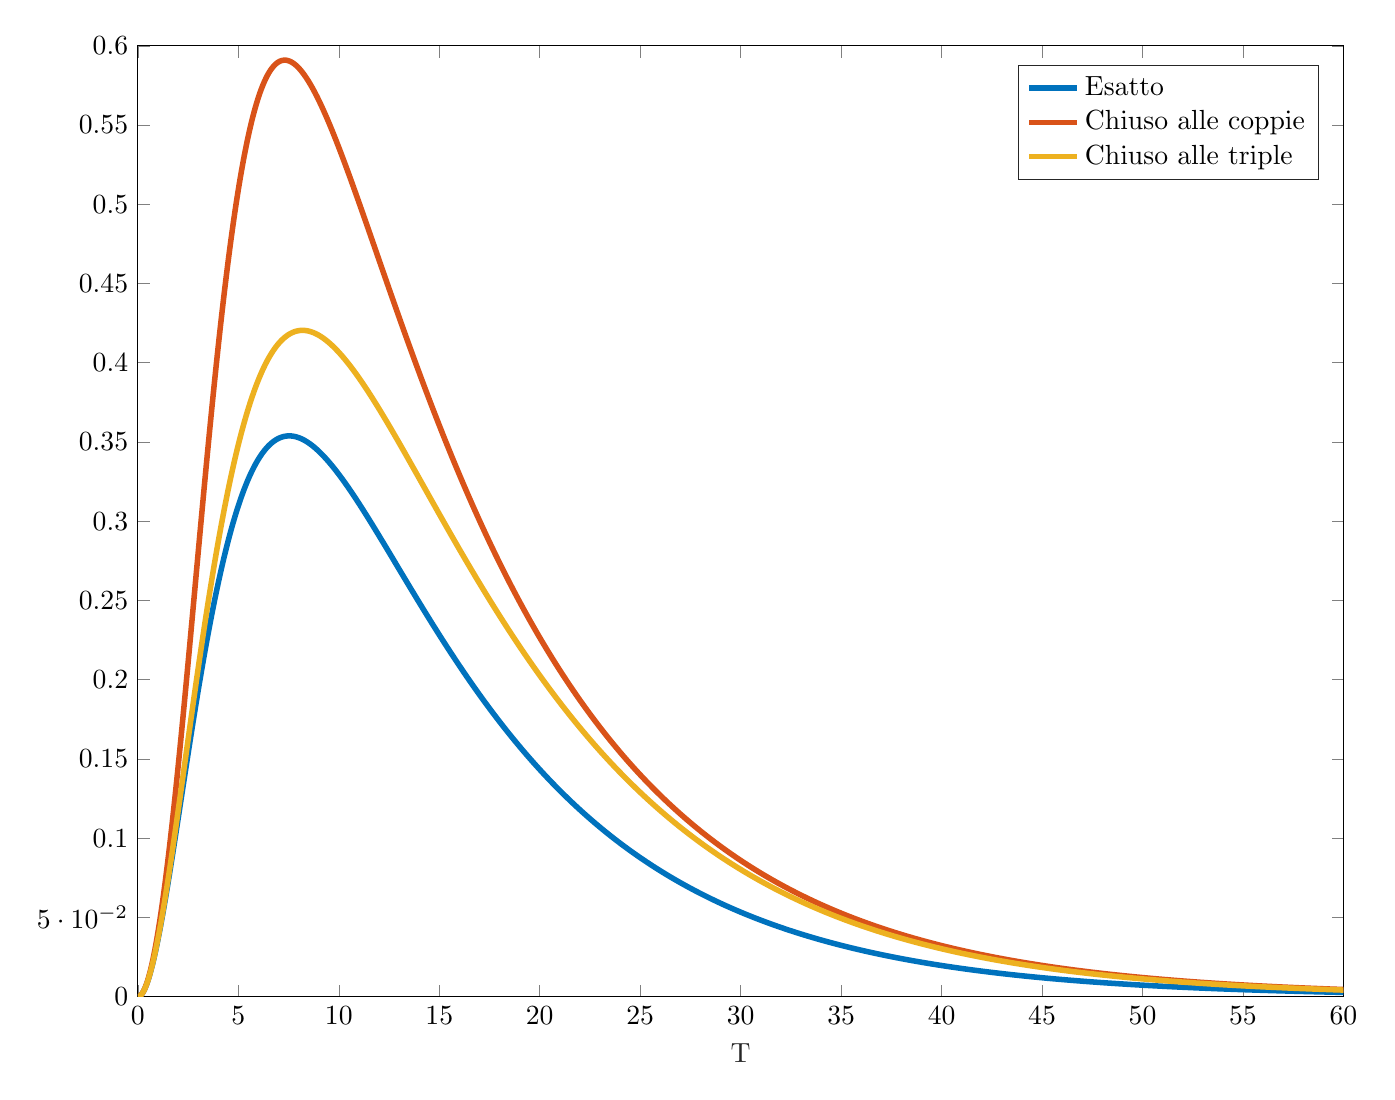
\begin{tikzpicture}

\begin{axis}[%
width=6.028in,
height=4.754in,
at={(1.011in,0.642in)},
scale only axis,
xmin=0,
xmax=60,
xlabel style={font=\color{white!15!black}},
xlabel={T},
ymin=0,
ymax=0.6,
axis background/.style={fill=white},
legend style={legend cell align=left, align=left, draw=white!15!black}
]
\addplot [color=mycolor1, line width=2.0pt]
  table[row sep=crcr]{%
0	0\\
0.00199053585276749	1.7822949683299e-07\\
0.00398107170553497	7.12633991639908e-07\\
0.00597160755830246	1.60278739921317e-06\\
0.00796214341106994	2.84826351211917e-06\\
0.0123567669950473	6.85404761850254e-06\\
0.0167513905790247	1.25850776445797e-05\\
0.0211460141630021	2.00367609805587e-05\\
0.0255406377469794	2.92045024183025e-05\\
0.0299388563931551	4.00933033485715e-05\\
0.0343370750393307	5.26917541687384e-05\\
0.0387352936855064	6.69952408030554e-05\\
0.043133512331682	8.29991469237719e-05\\
0.0475471725191068	0.000100763977079564\\
0.0519608327065316	0.000120231866818614\\
0.0563744928939564	0.000141398144414795\\
0.0607881530813811	0.000164258136209499\\
0.0652173199794049	0.000188896387840148\\
0.0696464868774286	0.000215230840277953\\
0.0740756537754524	0.000243256764792927\\
0.0785048206734761	0.000272969431043284\\
0.0829496187548012	0.000304477876436747\\
0.0873944168361263	0.000337675440822983\\
0.0918392149174515	0.000372557338934743\\
0.0962840129987766	0.000409118784214723\\
0.100744568101794	0.000447493511385649\\
0.105205123204811	0.00048755005287698\\
0.109665678307829	0.000529283567353318\\
0.114126233410846	0.000572689212512028\\
0.118602673075784	0.000617925628608725\\
0.123079112740721	0.000664836331901418\\
0.127555552405659	0.000713416425457245\\
0.132031992070596	0.000763661011700012\\
0.136524445545197	0.000815753845278292\\
0.141016899019798	0.000869513216851611\\
0.1455093524944	0.000924934174362011\\
0.150001805969001	0.000982011765433221\\
0.154510404254387	0.00104095506901093\\
0.159019002539772	0.00110155693968075\\
0.163527600825158	0.00116381237073368\\
0.168036199110544	0.00122771635546855\\
0.172561074936287	0.00129350350713688\\
0.17708595076203	0.00136094103361318\\
0.181610826587773	0.00143002387401335\\
0.186135702413515	0.00150074696778841\\
0.190676990405524	0.00157337067541191\\
0.195218278397533	0.0016476363445853\\
0.199759566389542	0.00172353886072682\\
0.204300854381551	0.00180107310991831\\
0.208858690959197	0.00188052541170688\\
0.213416527536843	0.0019616110411076\\
0.217974364114488	0.00204432483032052\\
0.222532200692134	0.0021286616125389\\
0.227106724202768	0.00221493388091906\\
0.231681247713401	0.00230283062264764\\
0.236255771224035	0.00239234661718764\\
0.240830294734669	0.0024834766453261\\
0.245421645441331	0.0025765595886291\\
0.250012996147992	0.00267125793099609\\
0.254604346854654	0.00276756639963606\\
0.259195697561315	0.00286547972341409\\
0.263804017673384	0.00296536338805228\\
0.268412337785452	0.0030668531577369\\
0.273020657897521	0.00316994370790795\\
0.27762897800959	0.0032746297159948\\
0.282254411746462	0.00338130348931587\\
0.286879845483334	0.00348957385422454\\
0.291505279220206	0.00359943543487873\\
0.296130712957079	0.00371088285776032\\
0.300773406613671	0.00382433547112046\\
0.305416100270264	0.00393937494346342\\
0.310058793926856	0.00405599584815389\\
0.314701487583449	0.00417419276121634\\
0.319361589521735	0.00429441229130397\\
0.324021691460022	0.00441620872887048\\
0.328681793398309	0.00453957659697822\\
0.333341895336596	0.00466451042168647\\
0.338019556071109	0.00479148429396836\\
0.342697216805623	0.00492002490358779\\
0.347374877540136	0.00505012672379765\\
0.35205253827465	0.00518178423118626\\
0.356747910447269	0.00531549922049169\\
0.361443282619888	0.00545077055855654\\
0.366138654792507	0.00558759266931946\\
0.370834026965126	0.00572595998039428\\
0.375547265516765	0.00586640221680881\\
0.380260504068404	0.00600839019523782\\
0.384973742620042	0.00615191829080272\\
0.389686981171681	0.00629698088264131\\
0.394418243246227	0.00644413584998692\\
0.399149505320772	0.00659282573459474\\
0.403880767395317	0.0067430448632684\\
0.408612029469863	0.00689478756717048\\
0.41336147459102	0.00704864010920734\\
0.418110919712177	0.00720401652597503\\
0.422860364833334	0.00736091109646086\\
0.427609809954491	0.0075193181043551\\
0.432377599961091	0.00767985242376575\\
0.437145389967691	0.00784189935773421\\
0.44191317997429	0.00800545313793538\\
0.44668096998089	0.00817050800109258\\
0.451467269141767	0.00833770766384279\\
0.456253568302644	0.00850640846349847\\
0.461039867463521	0.00867660458492832\\
0.465826166624398	0.00884829021839637\\
0.47063114173014	0.00902213815769364\\
0.475436116835881	0.00919747553893355\\
0.480241091941623	0.00937429650068697\\
0.485046067047365	0.00955259518726855\\
0.489869887370685	0.00973307370281882\\
0.494693707694006	0.00991502974813026\\
0.499517528017326	0.0100984574159869\\
0.504341348340647	0.0102833508052665\\
0.509184185682064	0.0104704415650874\\
0.51402702302348	0.0106589977253382\\
0.518869860364897	0.0108490133335296\\
0.523712697706314	0.0110404824436177\\
0.528574726619363	0.0112341664929077\\
0.533436755532412	0.011429303596298\\
0.53829878444546	0.0116258877565419\\
0.543160813358509	0.0118239129831912\\
0.548042211039569	0.0120241707405318\\
0.55292360872063	0.0122258689886733\\
0.55780500640169	0.01242900168613\\
0.56268640408275	0.0126335627985692\\
0.56758735048985	0.0128403740605406\\
0.572488296896949	0.0130486130330867\\
0.577389243304049	0.013258273631004\\
0.582290189711149	0.0134693497765985\\
0.587210867601438	0.0136826937191977\\
0.592131545491728	0.0138974523752264\\
0.597052223382018	0.0141136196162876\\
0.601972901272307	0.0143311893218511\\
0.606913496388328	0.0145510445083023\\
0.611854091504349	0.0147723011941749\\
0.61679468662037	0.0149949532084038\\
0.621735281736391	0.0152189943881514\\
0.626695982628195	0.0154453387607953\\
0.631656683519999	0.0156730712018817\\
0.636617384411802	0.0159021854982077\\
0.641578085303606	0.0161326754451591\\
0.646559083672327	0.0163654863400477\\
0.651540082041047	0.0165996716554555\\
0.656521080409768	0.0168352251365739\\
0.661502078778488	0.0170721405375458\\
0.666503569383853	0.0173113946798649\\
0.671505059989219	0.0175520093777441\\
0.676506550594584	0.0177939783353041\\
0.68150804119995	0.0180372952659821\\
0.686530221876942	0.0182829687696425\\
0.691552402553934	0.0185299887467229\\
0.696574583230927	0.0187783488608115\\
0.701596763907919	0.0190280427851802\\
0.706639835866396	0.0192801111661346\\
0.711682907824873	0.0195335117211375\\
0.71672597978335	0.0197882380737862\\
0.721769051741827	0.0200442838577301\\
0.72683321952555	0.0203027220311834\\
0.731897387309272	0.0205624778619397\\
0.736961555092995	0.0208235449341491\\
0.742025722876718	0.0210859168423846\\
0.747111194287107	0.021350699117281\\
0.752196665697496	0.0216167843151089\\
0.757282137107885	0.0218841659811192\\
0.762367608518274	0.0221528376713582\\
0.767474594900923	0.0224239377630902\\
0.772581581283573	0.0226963258255833\\
0.777688567666222	0.0229699953657403\\
0.782795554048871	0.0232449399016338\\
0.78792427039055	0.0235223309356013\\
0.793052986732229	0.0238009947701614\\
0.798181703073909	0.0240809248744226\\
0.803310419415588	0.0243621147290403\\
0.808461084325784	0.0246457692377514\\
0.81361174923598	0.0249306811586031\\
0.818762414146177	0.0252168439234676\\
0.823913079056373	0.0255042509761424\\
0.82908591482452	0.0257941408997806\\
0.834258750592667	0.0260852726284916\\
0.839431586360813	0.0263776395574727\\
0.84460442212896	0.0266712350942269\\
0.849799655005291	0.0269673317936489\\
0.854994887881621	0.0272646544721845\\
0.860190120757951	0.0275631964889205\\
0.865385353634282	0.0278629512156326\\
0.870603213699137	0.0281652254623746\\
0.875821073763992	0.0284687096429592\\
0.881038933828848	0.0287733970809315\\
0.886256793893703	0.0290792811129109\\
0.891497515445601	0.0293877031083246\\
0.896738236997499	0.0296973187726762\\
0.901978958549397	0.0300081213945414\\
0.907219680101295	0.0303201042759573\\
0.912483501408722	0.0306346436336498\\
0.917747322716149	0.0309503601752191\\
0.923011144023576	0.0312672471548477\\
0.928274965331004	0.0315852978405694\\
0.933562128954513	0.0319059236013823\\
0.938849292578023	0.0322277098403928\\
0.944136456201532	0.0325506497779706\\
0.949423619825042	0.0328747366487286\\
0.954734372782572	0.0332014172870096\\
0.960045125740102	0.0335292414767102\\
0.965355878697632	0.0338582024049715\\
0.970666631655162	0.0341882932735724\\
0.976001225418392	0.0345209966929383\\
0.981335819181621	0.034854826515271\\
0.98667041294485	0.0351897758950715\\
0.99200500670808	0.0355258380018755\\
0.997363697280812	0.0358645315353193\\
1.00272238785355	0.0362043341009664\\
1.00808107842628	0.0365452388212707\\
1.01343976899901	0.0368872388341203\\
1.0188228172289	0.037231889258643\\
1.02420586545878	0.0375776311216919\\
1.02958891368867	0.037924457514271\\
1.03497196191855	0.0382723615432202\\
1.04037963341625	0.0386229350696379\\
1.04578730491395	0.0389745822172536\\
1.05119497641164	0.0393272960462231\\
1.05660264790934	0.0396810696329432\\
1.06203521338424	0.0400375319217814\\
1.06746777885913	0.0403950497901334\\
1.07290034433402	0.0407536162679132\\
1.07833290980891	0.041113224401683\\
1.08379064506731	0.041475540557303\\
1.08924838032571	0.0418388940255831\\
1.09470611558411	0.0422032778068064\\
1.10016385084252	0.0425686849183151\\
1.1056470369148	0.0429368194907472\\
1.11113022298707	0.0433059728829442\\
1.11661340905935	0.0436761380661753\\
1.12209659513163	0.044047308029181\\
1.12760551858231	0.0444212250280102\\
1.13311444203298	0.0447961421268009\\
1.13862336548365	0.0451720522684289\\
1.14413228893432	0.0455489484136572\\
1.14966724184116	0.0459286112995448\\
1.15520219474799	0.0463092553376902\\
1.16073714765482	0.0466908734432023\\
1.16627210056166	0.0470734585494963\\
1.17183338076584	0.0474588302433864\\
1.17739466097002	0.0478451639129115\\
1.18295594117419	0.0482324524460456\\
1.18851722137837	0.0486206887494906\\
1.19410513262804	0.0490117316343535\\
1.19969304387772	0.049403717088219\\
1.20528095512739	0.0497966379725634\\
1.21086886637706	0.0501904871680156\\
1.21648371859449	0.0505871630988377\\
1.22209857081192	0.0509847619608945\\
1.22771342302936	0.0513832765898067\\
1.23332827524679	0.0517826998407763\\
1.23897038457538	0.0521849701387789\\
1.24461249390397	0.0525881434978711\\
1.25025460323256	0.0529922127284671\\
1.25589671256115	0.0533971706609938\\
1.26156640151281	0.0538049961141078\\
1.26723609046446	0.0542137045244657\\
1.27290577941612	0.0546232886779301\\
1.27857546836778	0.0550337413808108\\
1.28427306633634	0.0554470822701269\\
1.28997066430491	0.0558612857778406\\
1.29566826227347	0.056276344665923\\
1.30136586024204	0.0566922517172312\\
1.30709170327692	0.0571110677899438\\
1.31281754631181	0.0575307259056938\\
1.31854338934669	0.0579512188032283\\
1.32426923238158	0.0583725392426218\\
1.33002366371043	0.0587967897381747\\
1.33577809503928	0.0592218614633908\\
1.34153252636813	0.0596477471344669\\
1.34728695769699	0.0600744394893725\\
1.35307032782915	0.0605040831349718\\
1.35885369796131	0.060934526957224\\
1.36463706809348	0.0613657636504559\\
1.37042043822564	0.0617977859312162\\
1.37622881553645	0.0622324596390813\\
1.38203719284726	0.0626679110854667\\
1.38784557015807	0.0631041329597008\\
1.39365394746888	0.06354111797372\\
1.39948194569202	0.0639803388396922\\
1.40530994391516	0.0644203133789047\\
1.41113794213829	0.0648610342977984\\
1.41696594036143	0.0653024943257203\\
1.4228137248248	0.0657461887088551\\
1.42866150928816	0.0661906126324523\\
1.43450929375153	0.066635758821069\\
1.44035707821489	0.0670816200224627\\
1.44622478964653	0.0675297119422864\\
1.45209250107816	0.0679785091980472\\
1.45796021250979	0.0684280045335172\\
1.46382792394143	0.0688781907159599\\
1.46971570462452	0.06933060380475\\
1.4756034853076	0.0697836979560401\\
1.48149126599069	0.0702374659339126\\
1.48737904667378	0.0706919005262287\\
1.49328704060906	0.0711485580486936\\
1.49919503454433	0.0716058722941636\\
1.50510302847961	0.0720638360481231\\
1.51101102241489	0.0725224421201197\\
1.51693937480906	0.0729832669409242\\
1.52286772720322	0.0734447240819047\\
1.52879607959739	0.0739068063510373\\
1.53472443199155	0.0743695065806426\\
1.540673290528	0.0748344212698549\\
1.54662214906446	0.0752999438160608\\
1.55257100760091	0.0757660670508118\\
1.55851986613736	0.0762327838302813\\
1.56448937947106	0.0767017105536235\\
1.57045889280476	0.077171220613061\\
1.57642840613847	0.077641306864804\\
1.58239791947216	0.0781119621899579\\
1.58838823791446	0.0785848227682172\\
1.59437855635675	0.0790582421067338\\
1.60036887479904	0.0795322130874562\\
1.60635919324133	0.0800067286174983\\
1.61237046959671	0.0804834445995198\\
1.61838174595208	0.0809606947139292\\
1.62439302230746	0.0814384718694869\\
1.63040429866284	0.0819167690003855\\
1.63643668672632	0.082397261551219\\
1.6424690747898	0.0828782635571478\\
1.64850146285328	0.0833597679548181\\
1.65453385091676	0.0838417677065706\\
1.66058750665404	0.0843259577069938\\
1.66664116239132	0.0848106324386069\\
1.67269481812859	0.0852957848670103\\
1.67874847386587	0.0857814079837585\\
1.68482355500326	0.086269216004294\\
1.69089863614064	0.0867574839882173\\
1.69697371727803	0.087246204931149\\
1.70304879841541	0.0877353718549195\\
1.70914546464501	0.0882267181784857\\
1.71524213087462	0.088718499656472\\
1.72133879710422	0.0892107093155815\\
1.72743546333383	0.0897033402089795\\
1.73355387572031	0.090198144789141\\
1.73967228810678	0.0906933596762203\\
1.74579070049326	0.0911889779290641\\
1.75190911287974	0.0916849926332298\\
1.75804943463327	0.0921831751622365\\
1.76418975638681	0.0926817431148547\\
1.77033007814035	0.0931806895831316\\
1.77647039989388	0.0936800076860703\\
1.78263279664118	0.0941814876231251\\
1.78879519338848	0.0946833280674174\\
1.79495759013578	0.0951855221452476\\
1.80111998688309	0.0956880630101131\\
1.80730462566597	0.0961927595059203\\
1.81348926444885	0.0966977915621178\\
1.81967390323173	0.0972031523403108\\
1.82585854201462	0.0977088350295388\\
1.83206559217232	0.0982166670034985\\
1.83827264233002	0.0987248095632161\\
1.84447969248772	0.0992332559066485\\
1.85068674264543	0.0997419992594213\\
1.85691637550678	0.100252885380191\\
1.86314600836813	0.100764057086932\\
1.86937564122948	0.101275507615001\\
1.87560527409083	0.101787230227648\\
1.88185766319929	0.102301088936961\\
1.88811005230775	0.102815208209947\\
1.89436244141622	0.103329581320398\\
1.90061483052468	0.103844201570231\\
1.90689015093446	0.104360951030282\\
1.91316547134424	0.104877936011757\\
1.91944079175402	0.105395149827927\\
1.92571611216381	0.105912585820409\\
1.93201454150218	0.106432144006178\\
1.93831297084055	0.106951912653814\\
1.94461140017892	0.107471885117105\\
1.9509098295173	0.107992054778401\\
1.95723154808653	0.108514339491407\\
1.96355326665576	0.109036809592037\\
1.96987498522499	0.109559458475624\\
1.97619670379422	0.110082279566281\\
1.98254189319299	0.110607208325653\\
1.98888708259176	0.111132297386234\\
1.99523227199053	0.111657540185934\\
2.0015774613893	0.112182930191658\\
2.00794630624256	0.112710420381656\\
2.01431515109582	0.113238045776883\\
2.02068399594908	0.113765799858857\\
2.02705284080234	0.114293676138296\\
2.03344552746868	0.114823644906098\\
2.03983821413503	0.11535372377611\\
2.04623090080137	0.115883906274483\\
2.05262358746771	0.116414185956769\\
2.05904030495676	0.116946550292829\\
2.06545702244581	0.117478999623595\\
2.07187373993486	0.118011527520871\\
2.07829045742391	0.118544127586065\\
2.084731396657	0.119078804267171\\
2.0911723358901	0.119613540833507\\
2.0976132751232	0.120148330903553\\
2.1040542143563	0.12068316812559\\
2.11051956957009	0.12122007383553\\
2.11698492478388	0.121757014321785\\
2.12345027999767	0.12229398325053\\
2.12991563521146	0.122830974317928\\
2.13640560238783	0.123370025521238\\
2.1428955695642	0.123909086394997\\
2.14938553674057	0.124448150654087\\
2.15587550391694	0.124987212043569\\
2.16239028199053	0.125528325089654\\
2.16890506006412	0.12606942270586\\
2.17541983813771	0.126610498656792\\
2.1819346162113	0.127151546737412\\
2.18847440630977	0.1276946378012\\
2.19501419640825	0.128237688342795\\
2.20155398650673	0.128780692177532\\
2.20809377660521	0.129323643151286\\
2.21465878275268	0.129868628295239\\
2.22122378890015	0.130413547835157\\
2.22778879504762	0.130958395638113\\
2.23435380119508	0.131503165601899\\
2.24094422983074	0.132049960739475\\
2.24753465846639	0.132596665204097\\
2.25412508710205	0.133143272915586\\
2.2607155157377	0.13368977782465\\
2.2673315759421	0.134238298742397\\
2.27394763614649	0.134786703933639\\
2.28056369635089	0.135334987371944\\
2.28717975655528	0.13588314306194\\
2.29382166035897	0.136433305448228\\
2.30046356416266	0.136983327072242\\
2.30710546796636	0.137533201962302\\
2.31374737177005	0.138082924177949\\
2.32041533418655	0.13863464362859\\
2.32708329660306	0.13918619730137\\
2.33375125901957	0.139737579280361\\
2.34041922143607	0.140288783681014\\
2.34711345989709	0.140841975655293\\
2.3538076983581	0.141394976858727\\
2.36050193681912	0.141947781432133\\
2.36719617528013	0.142500383547867\\
2.37391691043736	0.143054963437569\\
2.3806376455946	0.143609327588407\\
2.38735838075183	0.144163470198944\\
2.39407911590907	0.144717385499429\\
2.40082657131283	0.145273268604641\\
2.40757402671659	0.145828911030314\\
2.41432148212035	0.146384307033746\\
2.42106893752412	0.146939450904073\\
2.42784333963791	0.147496552436712\\
2.4346177417517	0.148053388378842\\
2.4413921438655	0.148609953047493\\
2.44816654597929	0.149166240791669\\
2.4549681243632	0.149724475892727\\
2.4617697027471	0.150282420524358\\
2.46857128113101	0.15084006906431\\
2.47537285951492	0.151397415922448\\
2.48220184698832	0.15195669967724\\
2.48903083446173	0.15251566811806\\
2.49585982193513	0.153074315684363\\
2.50268880940853	0.153632636847854\\
2.50954544177924	0.154192884265536\\
2.51640207414995	0.154752791561409\\
2.52325870652066	0.155312353237623\\
2.53011533889137	0.155871563828708\\
2.53699985562036	0.156432689898206\\
2.54388437234935	0.156993451077035\\
2.55076888907833	0.157553841931022\\
2.55765340580732	0.158113857058503\\
2.5645660494942	0.158675776707669\\
2.57147869318108	0.159237306738586\\
2.57839133686796	0.159798441781744\\
2.58530398055484	0.160359176500262\\
2.59224499685821	0.16092180459078\\
2.59918601316159	0.161484018379066\\
2.60612702946496	0.162045812561256\\
2.61306804576833	0.162607181866231\\
2.62003768421203	0.163170433260129\\
2.62700732265572	0.163733245713629\\
2.63397696109942	0.164295613989492\\
2.64094659954311	0.164857532883338\\
2.64794511298781	0.165421322400728\\
2.65494362643251	0.165984648387643\\
2.6619421398772	0.166547505674449\\
2.6689406533219	0.167109889124479\\
2.67596829852112	0.167674131588995\\
2.68299594372033	0.168237885983242\\
2.69002358891955	0.168801147206172\\
2.69705123411877	0.169363910189805\\
2.70410827073433	0.169928520349816\\
2.71116530734989	0.170492617952379\\
2.71822234396545	0.17105619796601\\
2.72527938058101	0.17161925539239\\
2.73236607296869	0.172184148064524\\
2.73945276535637	0.172748503746725\\
2.74653945774405	0.173312317478044\\
2.75362615013173	0.173875584330795\\
2.76074276611797	0.174440674301384\\
2.76785938210422	0.175005202906485\\
2.77497599809046	0.175569165256664\\
2.78209261407671	0.176132556495839\\
2.78923942490227	0.17669775851668\\
2.79638623572783	0.177262374855673\\
2.80353304655339	0.177826400695873\\
2.81067985737896	0.178389831253774\\
2.81785713902212	0.178955060146569\\
2.82503442066529	0.179519679102398\\
2.83221170230846	0.180083683377779\\
2.83938898395163	0.18064706826275\\
2.84659701614953	0.181212238840401\\
2.85380504834743	0.181776775289409\\
2.86101308054533	0.182340672940731\\
2.86822111274323	0.182903927158917\\
2.87546017926332	0.18346895424622\\
2.88269924578341	0.184033323078808\\
2.88993831230351	0.184597029063049\\
2.8971773788236	0.185160067638973\\
2.90444776780364	0.185724866098001\\
2.91171815678368	0.186288982243949\\
2.91898854576373	0.186852411559568\\
2.92625893474377	0.187415149561337\\
2.93356093845992	0.187979634271801\\
2.94086294217606	0.188543412680673\\
2.94816494589221	0.189106480348063\\
2.95546694960836	0.189668832867867\\
2.96280086487659	0.190232918756606\\
2.97013478014483	0.190796274427175\\
2.97746869541306	0.191358895518011\\
2.9848026106813	0.191920777701399\\
2.99216873909201	0.192484379758104\\
2.99953486750271	0.193047227754021\\
3.00690099591342	0.193609317406891\\
3.01426712432413	0.194170644468351\\
3.02166577186631	0.194733677714194\\
3.02906441940849	0.195295933132706\\
3.03646306695067	0.195857406521901\\
3.04386171449286	0.196418093713738\\
3.05129319192691	0.196980473227474\\
3.05872466936097	0.19754205122545\\
3.06615614679503	0.198102823586926\\
3.07358762422909	0.198662786225152\\
3.08105224696524	0.199224427131048\\
3.0885168697014	0.199785242912944\\
3.09598149243755	0.200345229532325\\
3.1034461151737	0.200904382984697\\
3.11094420406679	0.201465200509217\\
3.11844229295988	0.202025169383599\\
3.12594038185297	0.202584285652525\\
3.13343847074605	0.203142545394727\\
3.14097035080817	0.203702454766353\\
3.14850223087028	0.204261492046012\\
3.1560341109324	0.204819653362557\\
3.16356599099451	0.205376934878918\\
3.17113199342146	0.205935851476072\\
3.17869799584842	0.206493872625496\\
3.18626399827537	0.20705099454119\\
3.19383000070233	0.207607213471252\\
3.20143046110215	0.208165052685973\\
3.20903092150198	0.208721973185447\\
3.21663138190181	0.209277971269797\\
3.22423184230164	0.209833043273262\\
3.2318671021242	0.210389720613092\\
3.23950236194676	0.210945456060259\\
3.24713762176933	0.21150024600199\\
3.25477288159189	0.212054086859637\\
3.26244328804483	0.212609517935818\\
3.27011369449776	0.213163984033911\\
3.2777841009507	0.213717481629223\\
3.28545450740363	0.214270007231193\\
3.29316041266953	0.214824107696851\\
3.30086631793543	0.215377220193082\\
3.30857222320133	0.215929341284257\\
3.31627812846722	0.216480467568877\\
3.32401989110489	0.217033153215368\\
3.33176165374256	0.217584827996945\\
3.33950341638023	0.218135488568027\\
3.3472451790179	0.218685131617155\\
3.35502316313618	0.21923631830838\\
3.36280114725446	0.219786471337052\\
3.37057913137275	0.220335587448621\\
3.37835711549103	0.220883663422646\\
3.38617169154667	0.221433267146064\\
3.3939862676023	0.221981814508943\\
3.40180084365794	0.22252930234875\\
3.40961541971357	0.223075727537046\\
3.41746696420648	0.223623664375271\\
3.42531850869938	0.224170522256531\\
3.43317005319229	0.224716298111303\\
3.4410215976852	0.225260988904131\\
3.44891049346576	0.225807175049859\\
3.45679938924632	0.226352259745611\\
3.46468828502688	0.226896240015862\\
3.47257718080744	0.227439112919129\\
3.48050381756295	0.227983464701382\\
3.48843045431847	0.2285266926458\\
3.49635709107398	0.229068793871853\\
3.50428372782949	0.229609765533017\\
3.51224850159594	0.230152199375446\\
3.52021327536239	0.23069348709924\\
3.52817804912884	0.23123362591986\\
3.53614282289529	0.231772613086733\\
3.54414613607264	0.232313045501611\\
3.55214944924998	0.232852309626045\\
3.56015276242733	0.233390402772492\\
3.56815607560468	0.233927322287327\\
3.57619833889781	0.234465669998337\\
3.58424060219095	0.235002827357494\\
3.59228286548408	0.235538791775251\\
3.60032512877721	0.236073560695929\\
3.60840675922679	0.236609740495042\\
3.61648838967638	0.237144707993296\\
3.62457002012596	0.237678460700149\\
3.63265165057554	0.23821099615887\\
3.64077307248204	0.238744924960261\\
3.64889449438855	0.239277619625967\\
3.65701591629505	0.239809077765467\\
3.66513733820155	0.240339297021984\\
3.67329898353354	0.240870891879215\\
3.68146062886554	0.241401230881812\\
3.68962227419754	0.241930311740289\\
3.69778391952953	0.242458132198835\\
3.70598622860803	0.242987310338433\\
3.71418853768653	0.243515211021843\\
3.72239084676502	0.244041832061637\\
3.73059315584352	0.244567171303982\\
3.73883657626523	0.245093850044177\\
3.74707999668693	0.24561922984592\\
3.75532341710863	0.246143308624868\\
3.76356683753034	0.24666608433019\\
3.77185182516863	0.247190181135091\\
3.78013681280692	0.247712957640202\\
3.78842180044522	0.248234411865297\\
3.79670678808351	0.248754541863568\\
3.80503380745825	0.249275974354245\\
3.81336082683299	0.249796065306283\\
3.82168784620774	0.250314812844608\\
3.83001486558248	0.25083221512747\\
3.83838438958511	0.251350901051855\\
3.84675391358775	0.251868224322941\\
3.85512343759039	0.252384183171852\\
3.86349296159302	0.252898775862928\\
3.8719054722877	0.253414633132844\\
3.88031798298237	0.253929106760488\\
3.88873049367705	0.25444219508423\\
3.89714300437172	0.254953896475545\\
3.90559899284027	0.255466843142865\\
3.91405498130882	0.255978385306229\\
3.92251096977737	0.25648852141231\\
3.93096695824593	0.256997249940768\\
3.93946692479213	0.2575072041959\\
3.94796689133833	0.258015733214279\\
3.95646685788454	0.258522835551945\\
3.96496682443074	0.259028509797801\\
3.97351127881372	0.259535389969321\\
3.98205573319669	0.260040824301765\\
3.99060018757967	0.260544811461612\\
3.99914464196265	0.261047350148068\\
4.00773410425464	0.26155107473823\\
4.01632356654662	0.262053333018832\\
4.02491302883861	0.262554123767866\\
4.0335024911306	0.263053445795917\\
4.04213749081375	0.263553933411006\\
4.05077249049689	0.264052934379626\\
4.05940749018004	0.264550447592377\\
4.06804248986318	0.265046471972299\\
4.07672356764034	0.265543641412176\\
4.08540464541749	0.266039304003458\\
4.09408572319465	0.26653345875044\\
4.10276680097181	0.267026104689711\\
4.11149450824228	0.26751987489828\\
4.12022221551276	0.268012118192356\\
4.12894992278323	0.26850283369104\\
4.1376776300537	0.268992020545566\\
4.14645252883691	0.269482310588696\\
4.15522742762012	0.269971053789234\\
4.16400232640333	0.270458249382202\\
4.17277722518654	0.270943896634584\\
4.18159988926615	0.271430625745956\\
4.19042255334575	0.271915788225688\\
4.19924521742536	0.272399383425849\\
4.20806788150496	0.272881410730293\\
4.21693889629988	0.273364498283558\\
4.22580991109479	0.273845999556575\\
4.23468092588971	0.2743259140196\\
4.24355194068463	0.274804241174484\\
4.2524719033702	0.275283606669781\\
4.26139186605577	0.275761366378113\\
4.27031182874135	0.276237519889067\\
4.27923179142692	0.276712066823633\\
4.28820131218307	0.277187629933685\\
4.29717083293922	0.277661567893043\\
4.30614035369538	0.278133880411788\\
4.31510987445153	0.2786045672312\\
4.32412957614907	0.279076247760928\\
4.33314927784661	0.279546283920541\\
4.34216897954416	0.280014675541787\\
4.3511886812417	0.280481422487404\\
4.36025919971018	0.280949140365308\\
4.36932971817866	0.281415194799323\\
4.37840023664715	0.281879585744049\\
4.38747075511563	0.282342313184861\\
4.39659274002011	0.282805988484664\\
4.40571472492458	0.283267981413586\\
4.41483670982906	0.283728292050282\\
4.42395869473353	0.284186920503955\\
4.43313280988389	0.284646473434564\\
4.44230692503424	0.28510432521523\\
4.45148104018459	0.285560476049881\\
4.46065515533495	0.286014926172754\\
4.469882079136	0.286470277074369\\
4.47910900293706	0.286923908196023\\
4.48833592673811	0.287375819868147\\
4.49756285053916	0.287826012451236\\
4.50684327607396	0.288277081772282\\
4.51612370160877	0.288726412833611\\
4.52540412714357	0.289174006093409\\
4.53468455267837	0.289619862039669\\
4.54401918924822	0.290066570383598\\
4.55335382581807	0.290511522139111\\
4.56268846238792	0.290954717893413\\
4.57202309895777	0.291396158263252\\
4.58141267108196	0.291838426309707\\
4.59080224320616	0.292278919591421\\
4.60019181533036	0.292717638825905\\
4.60958138745456	0.293154584759936\\
4.61902663678989	0.293592333326223\\
4.62847188612523	0.294028289104579\\
4.63791713546056	0.294462452944122\\
4.6473623847959	0.294894825722955\\
4.65686406984621	0.295327975717076\\
4.66636575489653	0.295759315054243\\
4.67586743994685	0.296188844716511\\
4.68536912499717	0.296616565714622\\
4.69492802222378	0.297045038153114\\
4.7044869194504	0.297471682220597\\
4.71404581667701	0.297896499033403\\
4.72360471390363	0.298319489736252\\
4.73320764525141	0.298742591428161\\
4.74281057659919	0.29916385254918\\
4.75241350794698	0.299583274345783\\
4.76201643929476	0.300000858092349\\
4.77165794452804	0.300418271397608\\
4.78129944976131	0.300833834515817\\
4.79094095499459	0.301247548821007\\
4.80058246022786	0.30165941571457\\
4.81026314694842	0.302071099118429\\
4.81994383366897	0.302480922979367\\
4.82962452038952	0.302888888798503\\
4.83930520711008	0.303294998103758\\
4.84902565638322	0.303700909065285\\
4.85874610565637	0.304104951399363\\
4.86846655492951	0.304507126733728\\
4.87818700420266	0.304907436722363\\
4.88794780523678	0.305307533203412\\
4.89770860627089	0.305705752241743\\
4.90746940730501	0.306102095591256\\
4.91723020833913	0.306496565031541\\
4.92703195872998	0.306890805485238\\
4.93683370912084	0.307283159948193\\
4.9466354595117	0.307673630300041\\
4.95643720990256	0.308062218445548\\
4.96628051524823	0.30845056177983\\
4.97612382059389	0.308837010840906\\
4.98596712593956	0.309221567633732\\
4.99581043128522	0.309604234187836\\
5.00569590732134	0.309986639829006\\
5.01558138335745	0.31036714317773\\
5.02546685939356	0.310745746363893\\
5.03535233542967	0.311122451541387\\
5.04528060635073	0.311498879344567\\
5.05520887727179	0.31187339709777\\
5.06513714819285	0.312246007055439\\
5.07506541911391	0.312616711495453\\
5.08503711889176	0.312987121774831\\
5.0950088186696	0.313355614506573\\
5.10498051844744	0.313722192069321\\
5.11495221822528	0.314086856864582\\
5.12496799094167	0.314451210382843\\
5.13498376365806	0.314813639113888\\
5.14499953637444	0.315174145560223\\
5.15501530909083	0.315532732246646\\
5.16507580953502	0.315890990213315\\
5.17513630997921	0.316247316409436\\
5.18519681042339	0.316601713461061\\
5.19525731086758	0.316954184015958\\
5.2053632039849	0.317306308044146\\
5.21546909710223	0.317656493573266\\
5.22557499021955	0.318004743352618\\
5.23568088333688	0.318351060152634\\
5.24583284576096	0.318697012290215\\
5.25598480818505	0.319041019453184\\
5.26613677060914	0.319383084513811\\
5.27628873303322	0.319723210364912\\
5.28648745229033	0.320062953042444\\
5.29668617154743	0.320400744521465\\
5.30688489080453	0.320736587796951\\
5.31708361006163	0.321070485883841\\
5.32732978639303	0.321403981952254\\
5.33757596272443	0.321735520848064\\
5.34782213905582	0.322065105688716\\
5.35806831538722	0.322392739611023\\
5.36836266133408	0.322719952301214\\
5.37865700728095	0.323045202093047\\
5.38895135322782	0.323368492226213\\
5.39924569917468	0.323689825959177\\
5.40958894010065	0.324010718873724\\
5.41993218102661	0.324329643411026\\
5.43027542195257	0.324646602932822\\
5.44061866287853	0.324961600819022\\
5.45101153706255	0.325276137909782\\
5.46140441124658	0.325588701389991\\
5.4717972854306	0.325899294743252\\
5.48219015961463	0.326207921470737\\
5.49263341945276	0.326516067049904\\
5.50307667929089	0.326822234029264\\
5.51351993912902	0.327126426014125\\
5.52396319896715	0.327428646626752\\
5.53445761187213	0.32773036536511\\
5.54495202477712	0.328030100756806\\
5.5554464376821	0.328327856528714\\
5.56594085058709	0.328623636424052\\
5.57648719831941	0.328918893302735\\
5.58703354605173	0.32921216232914\\
5.59757989378405	0.32950344735159\\
5.60812624151637	0.329792752234129\\
5.61872532103302	0.330081512542028\\
5.62932440054967	0.330368280732022\\
5.63992348006633	0.330653060773784\\
5.65052255958298	0.330935856652084\\
5.66117518401188	0.331218085984166\\
5.67182780844078	0.331498319171329\\
5.68248043286967	0.33177656030452\\
5.69313305729857	0.332052813489157\\
5.70384005671797	0.332328477736891\\
5.71454705613736	0.332602142049887\\
5.72525405555675	0.332873810640318\\
5.73596105497615	0.333143487734188\\
5.74672327665992	0.333412553060722\\
5.75748549834369	0.333679614898646\\
5.76824772002746	0.333944677581329\\
5.77900994171123	0.334207745455329\\
5.78982825023888	0.33447017826791\\
5.80064655876654	0.334730604272931\\
5.81146486729419	0.33498902792495\\
5.82228317582184	0.335245453691067\\
5.83315845473553	0.335501220650853\\
5.84403373364921	0.335754977717684\\
5.8549090125629	0.336006729467326\\
5.86578429147658	0.336256480487432\\
5.87671744355088	0.336505548482196\\
5.88765059562518	0.336752603730981\\
5.89858374769948	0.336997650930805\\
5.90951689977378	0.337240694789915\\
5.92050884813521	0.337483030925991\\
5.93150079649664	0.337723351694139\\
5.94249274485807	0.337961661912699\\
5.9534846932195	0.338197966410573\\
5.96453638108293	0.338433537972386\\
5.97558806894636	0.338667091774498\\
5.98663975680979	0.338898632756669\\
5.99769144467322	0.339128165868544\\
6.00880383710542	0.339356940322759\\
6.01991622953761	0.33958369485445\\
6.0310286219698	0.339808434524918\\
6.042141014402	0.340031164404669\\
6.05331509935885	0.340253109384269\\
6.0644891843157	0.340473032506196\\
6.07566326927256	0.340690938953445\\
6.08683735422941	0.340906833917525\\
6.09807414230094	0.34112191717886\\
6.10931093037248	0.341334976874208\\
6.12054771844401	0.341546018308435\\
6.13178450651555	0.341755046794229\\
6.14308503319571	0.341963236223625\\
6.15438555987588	0.342169400604244\\
6.16568608655605	0.342373545363039\\
6.17698661323621	0.342575675934077\\
6.18835193888863	0.342776939506329\\
6.19971726454106	0.342976176771615\\
6.21108259019348	0.343173393279219\\
6.2224479158459	0.343368594584821\\
6.23387912710053	0.343562900348393\\
6.24531033835517	0.343755178770374\\
6.2567415496098	0.343945435522649\\
6.26817276086443	0.344133676282783\\
6.2796709718506	0.344320992338856\\
6.29116918283678	0.344506280241196\\
6.30266739382295	0.3446895457846\\
6.31416560480912	0.344870794768814\\
6.32573195844141	0.345051089248496\\
6.33729831207371	0.345229354983671\\
6.34886466570601	0.345405597892395\\
6.36043101933831	0.34557982389693\\
6.37206668825559	0.345753064930601\\
6.38370235717287	0.345924276849353\\
6.39533802609016	0.346093465694883\\
6.40697369500744	0.34626063751234\\
6.41867988207414	0.346426793191705\\
6.43038606914084	0.346590919605371\\
6.44209225620754	0.346753022919096\\
6.45379844327423	0.346913109301326\\
6.46557638449348	0.347072147674652\\
6.47735432571273	0.347229156849865\\
6.48913226693197	0.34738414311724\\
6.50091020815122	0.347537112768972\\
6.51276117329228	0.347689001798229\\
6.52461213843333	0.347838861914338\\
6.53646310357439	0.347986699532597\\
6.54831406871544	0.348132521069439\\
6.56023936237899	0.34827722859338\\
6.57216465604253	0.348419907705689\\
6.58408994970607	0.348560564947234\\
6.59601524336962	0.348699206859221\\
6.608016207688	0.348836700574063\\
6.62001717200638	0.348972166594139\\
6.63201813632476	0.349105611586476\\
6.64401910064313	0.349237042217634\\
6.65609711612489	0.349367289630464\\
6.66817513160664	0.349495510279822\\
6.68025314708839	0.349621710959544\\
6.69233116257014	0.34974589846217\\
6.70448764976455	0.349868866852896\\
6.71664413695897	0.349989809625007\\
6.72880062415338	0.35010873369983\\
6.7409571113478	0.35022564599657\\
6.75319353351478	0.350341302386531\\
6.76542995568177	0.350454934515151\\
6.77766637784875	0.350566549432\\
6.78990280001574	0.350676154183678\\
6.80222066442117	0.350784465285752\\
6.8145385288266	0.350890753695281\\
6.82685639323203	0.350995026590879\\
6.83917425763746	0.351097291147327\\
6.85157511856051	0.351198223329069\\
6.86397597948357	0.351297134597388\\
6.87637684040662	0.351394032260806\\
6.88877770132968	0.351488923623136\\
6.90126316148383	0.351582442850922\\
6.91374862163799	0.351673943153817\\
6.92623408179214	0.351763431971179\\
6.93871954194629	0.351850916736759\\
6.95129125486549	0.351936988525761\\
6.96386296778468	0.352021043586897\\
6.97643468070388	0.352103089491349\\
6.98900639362307	0.352183133803785\\
7.00166606764739	0.352261723173576\\
7.0143257416717	0.352338298219637\\
7.02698541569601	0.352412866646038\\
7.03964508972033	0.35248543614941\\
7.05239448925109	0.352556507554677\\
7.06514388878186	0.352625567246547\\
7.07789328831262	0.35269262306312\\
7.09064268784339	0.352757682834109\\
7.10348363709426	0.352821200108428\\
7.11632458634514	0.352882708484697\\
7.12916553559601	0.352942215936261\\
7.14200648484689	0.352999730427116\\
7.15494087138423	0.353055656717681\\
7.16787525792157	0.353109577129229\\
7.18080964445891	0.353161499771656\\
7.19374403099625	0.353211432744524\\
7.20677380774895	0.353259730434468\\
7.21980358450165	0.353306025467192\\
7.23283336125435	0.353350326090535\\
7.24586313800706	0.353392640540994\\
7.25899032889946	0.353433271181923\\
7.27211751979186	0.353471902588617\\
7.28524471068426	0.353508543148348\\
7.29837190157667	0.353543201236019\\
7.31159860422458	0.353576125459926\\
7.32482530687249	0.353607054072537\\
7.3380520095204	0.353635995602149\\
7.35127871216831	0.35366295856364\\
7.36460710304072	0.353688135997108\\
7.37793549391314	0.353711321640607\\
7.39126388478556	0.35373252416516\\
7.40459227565797	0.353751752227301\\
7.41802461355885	0.353769141393143\\
7.43145695145972	0.35378454278743\\
7.4448892893606	0.353797965225733\\
7.45832162726148	0.353809417508032\\
7.47186025959003	0.35381897572486\\
7.48539889191859	0.353826550383868\\
7.49893752424715	0.353832150447124\\
7.51247615657571	0.353835784859974\\
7.52612352432791	0.353837468128741\\
7.53977089208011	0.35383717224701\\
7.55341825983232	0.353834906325425\\
7.56706562758452	0.353830679456752\\
7.58082427117841	0.353824442339191\\
7.5945829147723	0.353816230670197\\
7.60834155836619	0.353806053711221\\
7.62210020196009	0.353793920704649\\
7.63597276754062	0.353779716191476\\
7.64984533312116	0.353763541915731\\
7.66371789870169	0.35374540729206\\
7.67759046428223	0.353725321714818\\
7.69157971106386	0.353703101081804\\
7.70556895784549	0.353678915662666\\
7.71955820462712	0.353652775027794\\
7.73354745140875	0.353624688726041\\
7.7476562591015	0.35359440137702\\
7.76176506679424	0.353562154403563\\
7.77587387448699	0.353527957534551\\
7.78998268217974	0.353491820476033\\
7.80421406003167	0.353453413769418\\
7.81844543788359	0.353413052782555\\
7.83267681573552	0.353370747405752\\
7.84690819358745	0.353326507505157\\
7.86126528820976	0.353279926568395\\
7.87562238283208	0.353231396875446\\
7.8899794774544	0.353180928481199\\
7.90433657207672	0.353128531415017\\
7.91882267896367	0.353073718934074\\
7.93330878585062	0.353016963397563\\
7.94779489273757	0.352958275028351\\
7.96228099962452	0.352897664022361\\
7.97689957365268	0.352834560014442\\
7.99151814768085	0.352769518824661\\
8.00613672170902	0.352702550847506\\
8.02075529573718	0.352633666449067\\
8.03550996276884	0.352562208013739\\
8.0502646298005	0.352488818439648\\
8.06501929683216	0.352413508296835\\
8.07977396386382	0.352336288125432\\
8.09466853533245	0.352256409161658\\
8.10956310680107	0.352174605267211\\
8.12445767826969	0.352090887191922\\
8.13935224973832	0.352005265654149\\
8.15439073744049	0.35191689655096\\
8.16942922514267	0.351826608885338\\
8.18446771284484	0.351734413591478\\
8.19950620054702	0.351640321570483\\
8.2146928332504	0.351543388862558\\
8.22987946595378	0.351444544115197\\
8.24506609865717	0.351343798451908\\
8.26025273136055	0.351241162961424\\
8.27559197362809	0.351135588942912\\
8.29093121589562	0.351028109556618\\
8.30627045816316	0.350918736120719\\
8.32160970043069	0.35080747991687\\
8.33710627308224	0.350693182212918\\
8.35260284573378	0.350576985954716\\
8.36809941838533	0.350458902660925\\
8.38359599103687	0.35033894381186\\
8.39925489573158	0.350215834885747\\
8.41491380042629	0.350090834352842\\
8.430572705121	0.349963953938605\\
8.44623160981571	0.349835205328252\\
8.46205815432056	0.349703191942671\\
8.4778846988254	0.34956929402296\\
8.49371124333024	0.349433523508257\\
8.50953778783509	0.349295892295475\\
8.52553761739547	0.34915487488178\\
8.54153744695585	0.349011980121519\\
8.55753727651623	0.348867220175019\\
8.57353710607661	0.348720607158308\\
8.58971623619016	0.348570479122112\\
8.60589536630372	0.348418481030364\\
8.62207449641727	0.34826462527279\\
8.63825362653082	0.348108924192648\\
8.65461848330403	0.347949571096118\\
8.67098334007723	0.347788355324967\\
8.68734819685043	0.34762528950733\\
8.70371305362364	0.347460386222592\\
8.72018188980809	0.347292592831934\\
8.73665072599255	0.347122963961679\\
8.75311956217701	0.346951512283014\\
8.76958839836146	0.346778250417062\\
8.78614348346302	0.346602269421402\\
8.80269856856458	0.346424484650271\\
8.81925365366614	0.346244908771212\\
8.83580873876771	0.346063554400636\\
8.85245111606455	0.345879463883055\\
8.86909349336139	0.345693601480292\\
8.88573587065824	0.345505979853203\\
8.90237824795508	0.345316611610455\\
8.91910883699713	0.345124491786593\\
8.93583942603918	0.344930632176372\\
8.95257001508123	0.34473504543063\\
8.96930060412328	0.344537744146977\\
8.98612034063892	0.344337675962106\\
9.00294007715455	0.344135900289318\\
9.01975981367019	0.343932429766136\\
9.03657955018582	0.343727276975844\\
9.05348938408815	0.343519342098702\\
9.07039921799048	0.343309732223399\\
9.08730905189281	0.343098459970885\\
9.10421888579513	0.342885537906871\\
9.12121978296026	0.342669818681566\\
9.13822068012539	0.342452457130689\\
9.15522157729052	0.342233465855393\\
9.17222247445565	0.342012857400611\\
9.18931541587169	0.34178943683006\\
9.20640835728774	0.341564406781241\\
9.22350129870378	0.341337779832316\\
9.24059424011982	0.34110956850427\\
9.25778022278737	0.340878530213245\\
9.27496620545493	0.340645915457859\\
9.29215218812249	0.340411736790126\\
9.30933817079004	0.340176006703945\\
9.32661820779546	0.33993743491279\\
9.34389824480088	0.33969731982985\\
9.3611782818063	0.339455673977868\\
9.37845831881172	0.339212509820552\\
9.39583344002363	0.338966489311163\\
9.41320856123555	0.338718958833359\\
9.43058368244747	0.338469930877525\\
9.44795880365938	0.338219417874108\\
9.46543005570071	0.337966033966248\\
9.48290130774205	0.337711173556463\\
9.50037255978338	0.337454849099721\\
9.51784381182471	0.337197072990174\\
9.53541225878365	0.336936411508148\\
9.55298070574258	0.336674307126193\\
9.57054915270152	0.336410772260838\\
9.58811759966045	0.336145819266939\\
9.60578432346384	0.335877966511259\\
9.62345104726722	0.335608704585671\\
9.64111777107061	0.335338045865281\\
9.658784494874	0.335066002662677\\
9.67655059520445	0.334791045389405\\
9.6943166955349	0.334514712796998\\
9.71208279586536	0.334237017216182\\
9.72984889619581	0.333957970914343\\
9.74771549159443	0.33367599629714\\
9.76558208699305	0.333392680325064\\
9.78344868239167	0.333108035281541\\
9.80131527779029	0.332822073385855\\
9.81928350543996	0.332533168998582\\
9.83725173308963	0.332242957327157\\
9.8552199607393	0.331951450604816\\
9.87318818838897	0.33165866099987\\
9.89125920482513	0.331362914785707\\
9.90933022126129	0.33106589545762\\
9.92740123769745	0.330767615195801\\
9.94547225413361	0.330468086114752\\
9.96364723590061	0.330165586356312\\
9.9818222176676	0.329861847746837\\
9.99999719943459	0.329556882410648\\
10.0181721812016	0.329250702405639\\
10.0364523247657	0.328941537707949\\
10.0547324683298	0.328631168508127\\
10.0730126118939	0.328319606871834\\
10.0912927554579	0.328006864797582\\
10.1096792783833	0.327691124050822\\
10.1280658013086	0.327374213230236\\
10.146452324234	0.327056144340071\\
10.1648388471593	0.326736929316713\\
10.1833329877765	0.326414701684792\\
10.2018271283938	0.326091338480386\\
10.220321269011	0.325766851643594\\
10.2388154096282	0.325441253045974\\
10.257418428294	0.325112627928829\\
10.2760214469598	0.32478290180723\\
10.2946244656257	0.324452086554435\\
10.3132274842915	0.324120193974498\\
10.3319406634311	0.323785260991743\\
10.3506538425707	0.323449261633106\\
10.3693670217104	0.323112207702343\\
10.38808020085	0.322774110933356\\
10.4069048454226	0.322432959901597\\
10.4257294899953	0.322090777177057\\
10.4445541345679	0.321747574491356\\
10.4633787791406	0.321403363505629\\
10.4823162175897	0.321056084407615\\
10.5012536560388	0.320707808348525\\
10.5201910944879	0.320358546985234\\
10.539128532937	0.32000831190353\\
10.5581801172831	0.319654994873401\\
10.5772317016292	0.319300715656755\\
10.5962832859753	0.318945485833154\\
10.6153348703214	0.318589316910481\\
10.6345019773376	0.318230052199976\\
10.6536690843538	0.317869860114696\\
10.67283619137	0.317508752154346\\
10.6920032983861	0.317146739746381\\
10.7112873293394	0.316781617718252\\
10.7305713602926	0.31641560315882\\
10.7498553912458	0.316048707485413\\
10.769139422199	0.315680942042566\\
10.7885418041401	0.315310053136061\\
10.8079441860811	0.314938306568057\\
10.8273465680222	0.314565713671027\\
10.8467489499633	0.314192285704117\\
10.8662711360792	0.313815720418554\\
10.8857933221952	0.313438332362405\\
10.9053155083112	0.313060132780826\\
10.9248376944271	0.312681132845138\\
10.9444811647161	0.312298981718272\\
10.9641246350051	0.311916042727739\\
10.9837681052941	0.311532327028952\\
11.0034115755831	0.311147845702993\\
11.02317783773	0.310760199286193\\
11.0429440998769	0.310371799923671\\
11.0627103620238	0.309982658678693\\
11.0824766241707	0.309592786539725\\
11.102367213876	0.309199735384577\\
11.1222578035813	0.308805966207861\\
11.1421483932866	0.308411489978322\\
11.1620389829919	0.308016317589452\\
11.182055464688	0.3076179522278\\
11.202071946384	0.307218903770255\\
11.22208842808	0.306819183088694\\
11.2421049097761	0.306418800979306\\
11.2622488777205	0.30601521189653\\
11.282392845665	0.305610974640484\\
11.3025368136094	0.305206099983853\\
11.3226807815539	0.304800598623219\\
11.3429428732039	0.304392097920854\\
11.363204964854	0.303982984619114\\
11.3834670565041	0.303573269371919\\
11.4037291481542	0.303162962756851\\
11.4240073959591	0.302751747421538\\
11.444285643764	0.302339960742818\\
11.464563891569	0.301927613095044\\
11.4848421393739	0.301514714777566\\
11.5051410232308	0.301100855009188\\
11.5254399070878	0.300686463875284\\
11.5457387909448	0.300271551481933\\
11.5660376748017	0.299856127861473\\
11.5863613245615	0.299439695216151\\
11.6066849743212	0.299022769999474\\
11.627008624081	0.298605362059437\\
11.6473322738407	0.298187481171496\\
11.6676846007299	0.297768546422854\\
11.6880369276191	0.297349156792186\\
11.7083892545083	0.29692932187876\\
11.7287415813975	0.296509051210455\\
11.7491263024508	0.296087684298775\\
11.7695110235041	0.29566589916054\\
11.7898957445574	0.295243705154907\\
11.8102804656107	0.294821111570748\\
11.8307011258767	0.294397381546999\\
11.8511217861426	0.293973268982398\\
11.8715424464086	0.293548783003947\\
11.8919631066745	0.293123932669421\\
11.9124230970895	0.292697907685015\\
11.9328830875046	0.292271534933825\\
11.9533430779196	0.291844823318058\\
11.9738030683347	0.291417781671719\\
11.9943056417768	0.290989528968619\\
12.014808215219	0.290560962414048\\
12.0353107886612	0.290132090692246\\
12.0558133621033	0.289702922420238\\
12.0763616495731	0.289272508285524\\
12.0969099370428	0.288841813404089\\
12.1174582245125	0.288410846248554\\
12.1380065119823	0.287979615225276\\
12.1586035338403	0.287547105020278\\
12.1792005556983	0.287114346406892\\
12.1997975775563	0.286681347652032\\
12.2203945994143	0.286248116957265\\
12.2410432774846	0.285813575103965\\
12.2616919555548	0.285378816454681\\
12.2823406336251	0.284943849076133\\
12.3029893116954	0.284508680970584\\
12.3236924799435	0.284072170945912\\
12.3443956481917	0.283635475048971\\
12.3650988164398	0.283198601151438\\
12.385801984688	0.282761557061398\\
12.406562398648	0.28232314139858\\
12.4273228126081	0.281884570132866\\
12.4480832265682	0.281445850945713\\
12.4688436405282	0.281006991455828\\
12.4896639845707	0.280566731774383\\
12.5104843286133	0.280126346136845\\
12.5313046726558	0.279685842038975\\
12.5521250166983	0.279245226914598\\
12.5730079121072	0.278803183918352\\
12.5938908075161	0.278361044019681\\
12.614773702925	0.277918814532893\\
12.6356565983338	0.277476502711155\\
12.6566046110283	0.277032736180354\\
12.6775526237227	0.27658890123499\\
12.6985006364172	0.27614500501191\\
12.7194486491116	0.275701054587593\\
12.7404642942679	0.275255623424837\\
12.7614799394242	0.27481015179503\\
12.7824955845805	0.274364646661309\\
12.8035112297368	0.273919114927201\\
12.8245969793381	0.273472077130889\\
12.8456827289394	0.273025026298414\\
12.8667684785407	0.272577969222742\\
12.887854228142	0.272130912637966\\
12.9090125143938	0.271682325353936\\
12.9301708006455	0.271233751970191\\
12.9513290868973	0.270785199112861\\
12.972487373149	0.270336673349927\\
12.9937205946389	0.269886592856556\\
13.0149538161287	0.269436552726247\\
13.0361870376186	0.268986559421443\\
13.0574202591085	0.268536619347148\\
13.0787307850171	0.268085101074268\\
13.1000413109258	0.267633649173042\\
13.1213518368345	0.267182269945202\\
13.1426623627431	0.266730969635736\\
13.1640525369264	0.266278068179563\\
13.1854427111097	0.265825258667767\\
13.206832885293	0.265372547244184\\
13.2282230594763	0.264919939996587\\
13.2496952043377	0.264465709133069\\
13.271167349199	0.26401159536803\\
13.2926394940603	0.263557604690073\\
13.3141116389217	0.26310374303241\\
13.3356680588802	0.262648235733724\\
13.3572244788388	0.262192870285263\\
13.3787808987974	0.261737652522924\\
13.400337318756	0.261282588227862\\
13.4219803036483	0.260825856675449\\
13.4436232885406	0.260369291338023\\
13.4652662734329	0.259912897901161\\
13.4869092583252	0.259456681996344\\
13.5086410871513	0.258998777582328\\
13.5303729159775	0.258541063375628\\
13.5521047448036	0.258083544913769\\
13.5738365736297	0.257626227680816\\
13.5956595174591	0.257167201023304\\
13.6174824612885	0.256708388206808\\
13.639305405118	0.256249794622949\\
13.6611283489474	0.255791425610518\\
13.6830446722324	0.255331326598827\\
13.7049609955174	0.254871464716296\\
13.7268773188025	0.254411845210682\\
13.7487936420875	0.253952473277529\\
13.770805608124	0.253491351027005\\
13.7928175741606	0.253030488860713\\
13.8148295401972	0.252569891884488\\
13.8368415062338	0.252109565152556\\
13.858951377984	0.251647468054225\\
13.8810612497342	0.251185653674\\
13.9031711214845	0.250724126977625\\
13.9252809932347	0.250262892879839\\
13.9474910360997	0.249799868606433\\
13.9697010789646	0.249337149375126\\
13.9919111218296	0.248874740013322\\
14.0141211646945	0.24841264529801\\
14.0364336494706	0.247948740803995\\
14.0587461342466	0.247485163377036\\
14.0810586190226	0.247021917707853\\
14.1033711037986	0.246559008437337\\
14.1257883079129	0.246094269992824\\
14.1482055120272	0.245629880351633\\
14.1706227161414	0.245165844069373\\
14.1930399202557	0.244702165652403\\
14.2155641320733	0.244236638811448\\
14.2380883438909	0.24377148223137\\
14.2606125557085	0.243306700334161\\
14.283136767526	0.242842297493138\\
14.3057702854045	0.242376027169449\\
14.3284038032829	0.241910148294966\\
14.3510373211614	0.241444665159483\\
14.3736708390398	0.240979582004689\\
14.3964159769655	0.240512612409653\\
14.4191611148912	0.240046055192162\\
14.4419062528169	0.239579914511159\\
14.4646513907425	0.239114194478043\\
14.4875104777278	0.238646569186628\\
14.510369564713	0.238179376949912\\
14.5332286516983	0.237712621797264\\
14.5560877386835	0.237246307711065\\
14.5790631229979	0.236778069627075\\
14.6020385073122	0.236310285032328\\
14.6250138916265	0.235842957827827\\
14.6479892759408	0.235376091868143\\
14.6710833264109	0.234907283249108\\
14.6941773768809	0.234438948319511\\
14.7172714273509	0.233971090853135\\
14.740365477821	0.23350371457788\\
14.7635805844029	0.233034377073634\\
14.7867956909849	0.232565533232605\\
14.8100107975669	0.232097186702443\\
14.8332259041488	0.231629341085457\\
14.8565644820063	0.231159515704894\\
14.8799030598637	0.230690203742689\\
14.9032416377212	0.230221408721382\\
14.9265802155787	0.229753134118713\\
14.9500447068131	0.229282861244211\\
14.9735091980476	0.228813121332111\\
14.996973689282	0.228343917780809\\
15.0204381805165	0.227875253944443\\
15.0440310551214	0.22740457336136\\
15.0676239297264	0.226934445080915\\
15.0912168043314	0.226464872378272\\
15.1148096789363	0.225995858484872\\
15.1385334385982	0.225524809353817\\
15.16225719826	0.225054331669009\\
15.1859809579218	0.224584428583235\\
15.2097047175837	0.224115103206098\\
15.2335618956234	0.223643724112375\\
15.2574190736632	0.223172935418788\\
15.281276251703	0.222702740156559\\
15.3051334297427	0.222233141314249\\
15.3291265950906	0.221761470236936\\
15.3531197604384	0.221290408330777\\
15.3771129257863	0.22081995850618\\
15.4011060911341	0.220350123631419\\
15.4252378496272	0.21987819796609\\
15.4493696081203	0.219406900066727\\
15.4735013666134	0.218936232723627\\
15.4976331251065	0.218466198685481\\
15.5219061221034	0.217994055241169\\
15.5461791191004	0.217522557987992\\
15.5704521160973	0.217051709596792\\
15.5947251130942	0.216581512697327\\
15.619142035055	0.216109187714214\\
15.6435589570157	0.215637527184182\\
15.6679758789765	0.215166533659221\\
15.6923928009372	0.214696209650766\\
15.7169563780926	0.214223738797083\\
15.741519955248	0.213751950501544\\
15.7660835324033	0.213280847197849\\
15.7906471095587	0.212810431279663\\
15.8153601179615	0.212337849661332\\
15.8400731263644	0.211865968555567\\
15.8647861347672	0.211394790278288\\
15.88949914317	0.210924317105906\\
15.9143644081624	0.210451659249894\\
15.9392296731548	0.209979719716455\\
15.9640949381471	0.209508500704202\\
15.9889602031395	0.209038004372754\\
16.0139806003288	0.20856530425909\\
16.039000997518	0.208093340139683\\
16.0640213947072	0.207622114096256\\
16.0890417918965	0.207151628172058\\
16.1142202516767	0.206678919199335\\
16.1393987114569	0.206206963760384\\
16.1645771712372	0.205735763820411\\
16.1897556310174	0.205265321306671\\
16.2150951374624	0.204792636365007\\
16.2404346439074	0.204320722370353\\
16.2657741503524	0.203849581171733\\
16.2911136567974	0.203379214580735\\
16.3166172552097	0.202906585963\\
16.342120853622	0.202434745585401\\
16.3676244520343	0.201963695181062\\
16.3931280504465	0.201493436446194\\
16.4187988465862	0.201020895917179\\
16.4444696427259	0.200549160807247\\
16.4701404388656	0.200078232733864\\
16.4958112350053	0.199608113278099\\
16.5216524004798	0.199135692030019\\
16.5474935659542	0.198664093271874\\
16.5733347314287	0.198193318505666\\
16.5991758969032	0.197723369197523\\
16.6251906694304	0.197251097901986\\
16.6512054419577	0.196779666065064\\
16.677220214485	0.196309075073445\\
16.7032349870123	0.195839326278464\\
16.7294266758655	0.195367235044793\\
16.7556183647187	0.194896000142334\\
16.781810053572	0.194425622842562\\
16.8080017424252	0.193956104382126\\
16.8343737319713	0.193484222753421\\
16.8607457215174	0.193013214238582\\
16.8871177110636	0.19254307999393\\
16.9134897006097	0.192073821141484\\
16.9400454511807	0.191602178140289\\
16.9666012017517	0.19113142495169\\
16.9931569523226	0.190661562616863\\
17.0197127028936	0.190192592143212\\
17.0464557582069	0.18972121620201\\
17.0731988135202	0.189250746694543\\
17.0999418688336	0.188781184546807\\
17.1266849241469	0.188312530651552\\
17.1536189111414	0.187841449681257\\
17.1805528981359	0.187371291694387\\
17.2074868851304	0.186902057501672\\
17.2344208721249	0.186433747881126\\
17.2615495082445	0.18596298920981\\
17.2886781443641	0.185493170006616\\
17.3158067804836	0.185024290966868\\
17.3429354166032	0.184556352753713\\
17.3702625121198	0.184085943156115\\
17.3975896076364	0.183616489452767\\
17.424916703153	0.183147992223406\\
17.4522437986696	0.182680452016127\\
17.4797732620512	0.182210417692643\\
17.5073027254328	0.181741355637584\\
17.5348321888143	0.181273266314865\\
17.5623616521959	0.18080615015729\\
17.5900974943972	0.180336516735164\\
17.6178333365984	0.179867871910412\\
17.6455691787997	0.179400216030828\\
17.6733050210009	0.178933549413647\\
17.7012513604556	0.178464341939502\\
17.7291976999103	0.17799613935333\\
17.757144039365	0.177528941886463\\
17.7850903788197	0.177062749740218\\
17.8132514459017	0.176593992685139\\
17.8414125129837	0.176126256777279\\
17.8695735800657	0.175659542131107\\
17.8977346471477	0.175193848831625\\
17.9261147917276	0.174725566048494\\
17.9544949363076	0.174258320647813\\
17.9828750808876	0.173792112626722\\
18.0112552254676	0.173326941953454\\
18.0398589202161	0.172859156709772\\
18.0684626149646	0.172392425067112\\
18.097066309713	0.171926746904769\\
18.1256700044615	0.171462122073685\\
18.1545018545664	0.170994856982842\\
18.1833337046712	0.170528661702789\\
18.212165554776	0.170063535994386\\
18.2409974048809	0.169599479590711\\
18.2700621491713	0.169132756689052\\
18.2991268934616	0.168667119806848\\
18.328191637752	0.168202568585879\\
18.3572563820424	0.167739102640708\\
18.3865589068877	0.167272943261937\\
18.4158614317331	0.166807886118683\\
18.4451639565785	0.166343930732923\\
18.4744664814239	0.165881076599998\\
18.5040118216459	0.165415501465753\\
18.5335571618679	0.164951044798798\\
18.56310250209	0.164487706000521\\
18.592647842312	0.164025484446255\\
18.622441195706	0.163560513544633\\
18.6522345491	0.163096677366938\\
18.682027902494	0.162633975193102\\
18.711821255888	0.162172406277592\\
18.74186798467	0.161708058955891\\
18.771914713452	0.161244862648605\\
18.801961442234	0.160782816513268\\
18.8320081710161	0.160321919682543\\
18.8623138179204	0.159858214516622\\
18.8926194648247	0.159395676699381\\
18.922925111729	0.158934305264931\\
18.9532307586333	0.158474099223113\\
18.9838010512769	0.158011054078154\\
19.0143713439205	0.157549192669883\\
19.0449416365641	0.157088513907871\\
19.0755119292076	0.156629016678033\\
19.1063527942164	0.156166648626261\\
19.1371936592252	0.155705480763656\\
19.1680345242339	0.155245511874046\\
19.1988753892427	0.154786740718226\\
19.2299929618915	0.154325066035213\\
19.2611105345403	0.153864608069466\\
19.2922281071891	0.153405365477768\\
19.3233456798379	0.152947336894498\\
19.3547463174076	0.152486371008928\\
19.3861469549774	0.152026638456174\\
19.4175475925471	0.151568137764568\\
19.4489482301169	0.151110867440677\\
19.4806385226382	0.150650624933405\\
19.5123288151595	0.150191632474245\\
19.5440191076808	0.149733888461563\\
19.5757094002021	0.149277391272611\\
19.6076961882754	0.148817885783112\\
19.6396829763487	0.148359647170064\\
19.671669764422	0.147902673700236\\
19.7036565524953	0.147446963619945\\
19.7359469398787	0.146988207842549\\
19.768237327262	0.146530735896854\\
19.8005277146453	0.146074545916278\\
19.8328181020287	0.145619636014457\\
19.8654194755566	0.145161641602308\\
19.8980208490846	0.14470494811902\\
19.9306222226126	0.144249553562765\\
19.9632235961405	0.143795455912625\\
19.9961436388709	0.143338233493068\\
20.0290636816012	0.142882329256992\\
20.0619837243316	0.142427741065301\\
20.0949037670619	0.141974466760502\\
20.1281504830269	0.141518025802336\\
20.1613971989918	0.14106292045676\\
20.1946439149567	0.140609148445218\\
20.2278906309217	0.140156707471478\\
20.2614723645969	0.139701056245814\\
20.2950540982721	0.139246758254361\\
20.3286358319473	0.13879381107676\\
20.3622175656225	0.138342212275705\\
20.3961430262838	0.137887357768278\\
20.4300684869452	0.137433874328594\\
20.4639939476066	0.136981759391966\\
20.497919408268	0.136531010377504\\
20.5321976950164	0.136076958213675\\
20.5664759817649	0.135624295183814\\
20.6007542685134	0.135173018576186\\
20.6350325552618	0.134723125663622\\
20.6696731863085	0.134269879999803\\
20.7043138173553	0.133818041791335\\
20.738954448402	0.133367608176514\\
20.7735950794487	0.132918576278987\\
20.8086080231198	0.132466139697992\\
20.8436209667909	0.13201512917314\\
20.878633910462	0.131565541689607\\
20.9136468541332	0.131117374218728\\
20.949042565344	0.130665747583137\\
20.9844382765548	0.130215565910307\\
21.0198339877656	0.129766826028907\\
21.0552296989764	0.129319524754587\\
21.0910191546516	0.128868707106246\\
21.1268086103268	0.128419353661571\\
21.162598066002	0.127971461089061\\
21.1983875216773	0.127525026045043\\
21.234582265905	0.127075014415483\\
21.2707770101326	0.126626486596\\
21.3069717543603	0.126179439090965\\
21.343166498588	0.125733868393463\\
21.3797786897193	0.125284657631583\\
21.4163908808506	0.12483695068577\\
21.453003071982	0.124390743891995\\
21.4896152631133	0.12394603357585\\
21.5266577262528	0.123497616153326\\
21.5637001893923	0.123050722989729\\
21.6007426525319	0.122605350248009\\
21.6377851156714	0.122161494081665\\
21.6752714017348	0.121713859868044\\
21.7127576877983	0.121267770834052\\
21.7502439738617	0.120823222964597\\
21.7877302599251	0.12038021223611\\
21.8256747161126	0.119933348193961\\
21.8636191723001	0.11948805077547\\
21.9015636284876	0.119044315782058\\
21.9395080846751	0.11860213900767\\
21.9779259262067	0.118156028938427\\
22.0163437677384	0.117711507510204\\
22.0547616092701	0.117268570335004\\
22.0931794508017	0.1168272130184\\
22.1320868496398	0.116381837180468\\
22.1709942484778	0.115938072630051\\
22.2099016473158	0.115495914783276\\
22.2488090461539	0.115055359050922\\
22.2882232273236	0.114610693775138\\
22.3276374084934	0.114167663124606\\
22.3670515896632	0.113726262312512\\
22.4064657708329	0.113286486547827\\
22.4464051256478	0.112842503755618\\
22.4863444804626	0.112400179687296\\
22.5262838352775	0.111959509345371\\
22.5662231900924	0.111520487729324\\
22.6067074061995	0.111077154373807\\
22.6471916223066	0.110635504680155\\
22.6876758384138	0.110195533431708\\
22.7281600545209	0.109757235410015\\
22.7692102626757	0.109314512860348\\
22.8102604708306	0.108873499838312\\
22.8513106789854	0.108434190898714\\
22.8923608871403	0.107996580595874\\
22.9339998357608	0.107554423866995\\
22.9756387843813	0.107114003559847\\
23.0172777330018	0.106675313990364\\
23.0589166816223	0.106238349475361\\
23.1011689388352	0.105796706338301\\
23.143421196048	0.105356827660136\\
23.1856734532609	0.104918707506455\\
23.2279257104737	0.104482339945179\\
23.2707449436263	0.104041898791061\\
23.3135641767789	0.103603245321121\\
23.3563834099314	0.103166373369395\\
23.399202643084	0.102731276773756\\
23.4425351018712	0.102292766276092\\
23.4858675606585	0.101856061262634\\
23.5292000194457	0.101421155359805\\
23.5725324782329	0.1009880421994\\
23.6163923812599	0.100551476271586\\
23.6602522842869	0.100116733883273\\
23.704112187314	0.0996838084484594\\
23.747972090341	0.0992526933881005\\
23.7923730104802	0.0988180977595603\\
23.8367739306194	0.0983853438969392\\
23.8811748507586	0.0979544249972511\\
23.9255757708978	0.0975253342661019\\
23.9705318120247	0.0970927344967212\\
24.0154878531517	0.0966619949036958\\
24.0604438942787	0.0962331084622384\\
24.1053999354057	0.095806068157843\\
24.1509257391711	0.0953754898553352\\
24.1964515429365	0.094946790335303\\
24.2419773467019	0.0945199623460769\\
24.2875031504673	0.0940949986480146\\
24.3336139249026	0.0936664674796713\\
24.3797246993379	0.0932398339077524\\
24.4258354737732	0.0928150904483447\\
24.4719462482085	0.0923922296313692\\
24.518657797687	0.091965771341273\\
24.5653693471654	0.0915412296819874\\
24.6120808966439	0.0911185969316982\\
24.6587924461223	0.0906978653842966\\
24.7061212033434	0.0902735058107984\\
24.7534499605645	0.0898510821360418\\
24.8007787177855	0.0894305863943395\\
24.8481074750066	0.0890120106376493\\
24.8960705351928	0.0885897757309496\\
24.944033595379	0.0881694962381081\\
24.9919966555653	0.0877511639432586\\
25.0399597157515	0.087334770650193\\
25.0885748730688	0.0869146864915529\\
25.1371900303861	0.0864965775232734\\
25.1858051877034	0.0860804352726497\\
25.2344203450208	0.0856662512887253\\
25.2837061315614	0.0852483441100048\\
25.332991918102	0.0848324321743328\\
25.3822777046427	0.0844185067451287\\
25.4315634911833	0.0840065591097339\\
25.4815392186928	0.083590855313604\\
25.5315149462023	0.0831771671048343\\
25.5814906737117	0.0827654854755308\\
25.6314664012212	0.0823558014439828\\
25.6821522057685	0.0819423276251533\\
25.7328380103157	0.081530890045737\\
25.783523814863	0.0811214794186615\\
25.8342096194102	0.0807140864853939\\
25.8856265092156	0.0803028694532214\\
25.9370433990211	0.0798937096370933\\
25.9884602888265	0.0794865974624389\\
26.0398771786319	0.0790815233856831\\
26.0920470854784	0.078672590187033\\
26.144216992325	0.078265735523248\\
26.1963868991715	0.0778609495234529\\
26.2485568060181	0.0774582223503324\\
26.3015026403881	0.077051600294147\\
26.3544484747581	0.076647078452268\\
26.4073943091281	0.0762446466481909\\
26.4603401434981	0.07584429474165\\
26.5140858539001	0.0754400114242948\\
26.5678315643021	0.0750378503806181\\
26.6215772747041	0.074637801118606\\
26.6753229851061	0.0742398531852867\\
26.7298936218998	0.073837936517322\\
26.7844642586936	0.0734381645825868\\
26.8390348954873	0.073040526563084\\
26.893605532281	0.0726450116827938\\
26.9490273164448	0.0722454899170574\\
27.0044491006085	0.0718481357655304\\
27.0598708847722	0.0714529380731226\\
27.1152926689359	0.0710598857297983\\
27.1715930662283	0.0706627874909822\\
27.2278934635207	0.0702678801911074\\
27.2841938608131	0.0698751523261976\\
27.3404942581055	0.0694845924405614\\
27.3972810276665	0.0690928431203641\\
27.4540677972275	0.0687032761377449\\
27.5108545667884	0.068315879886813\\
27.5676413363494	0.0679306428118508\\
27.6246835621125	0.0675458349084736\\
27.6817257878755	0.0671631824309577\\
27.7387680136386	0.0667826738197535\\
27.7958102394016	0.0664042975664842\\
27.8531117250382	0.0660263369381133\\
27.9104132106748	0.0656505049712226\\
27.9677146963114	0.0652767901556355\\
28.025016181948	0.064905181033275\\
28.0825792753208	0.0645339839774115\\
28.1401423686935	0.06416488886513\\
28.1977054620663	0.0637978842393118\\
28.2552685554391	0.0634329586957896\\
28.3130956457549	0.0630684414838394\\
28.3709227360708	0.0627059995581774\\
28.4287498263866	0.0623456215181731\\
28.4865769167025	0.0619872960169281\\
28.5446704260258	0.0616293750069479\\
28.602763935349	0.0612735026991268\\
28.6608574446723	0.0609196677525173\\
28.7189509539956	0.0605678588806179\\
28.7773133374	0.0602164505671156\\
28.8356757208045	0.0598670644565151\\
28.8940381042089	0.0595196892705235\\
28.9524004876134	0.0591743137859449\\
29.0110342352743	0.0588293348349641\\
29.0696679829352	0.05848635168353\\
29.1283017305961	0.0581453531187652\\
29.186935478257	0.0578063279834804\\
29.2458431140456	0.0574676952861395\\
29.3047507498342	0.0571310320910462\\
29.3636583856228	0.0567963272533004\\
29.4225660214114	0.056463569684225\\
29.4817501049045	0.0561312003868377\\
29.5409341883977	0.0558007744100075\\
29.6001182718908	0.0554722806791852\\
29.659302355384	0.0551457081765261\\
29.7187654815208	0.0548195197221992\\
29.7782286076576	0.0544952485311762\\
29.8376917337944	0.0541728836014547\\
29.8971548599312	0.0538524139881685\\
29.9568996607722	0.0535323241440343\\
30.0166444616132	0.0532141256386678\\
30.0763892624543	0.0528978075446413\\
30.1361340632953	0.0525833589920476\\
30.1961632086509	0.0522692858810186\\
30.2561923540065	0.0519570783246248\\
30.316221499362	0.051646725471883\\
30.3762506447176	0.0513382165296689\\
30.436566841334	0.051030078667388\\
30.4968830379503	0.0507237807230529\\
30.5571992345667	0.0504193119238446\\
30.617515431183	0.0501166615551006\\
30.6781214246657	0.049814377870201\\
30.7387274181483	0.0495139086205949\\
30.799333411631	0.0492152431132072\\
30.8599394051136	0.0489183707133763\\
30.9208379817972	0.0486218605670439\\
30.9817365584807	0.0483271395335574\\
31.0426351351642	0.0480341970010315\\
31.1035337118477	0.0477430224162134\\
31.1647276970968	0.047452205637703\\
31.2259216823458	0.0471631528153517\\
31.2871156675948	0.0468758534197844\\
31.3483096528438	0.0465902969804433\\
31.4098019130839	0.0463050938819942\\
31.4712941733241	0.046021629753973\\
31.5327864335642	0.0457398941507182\\
31.5942786938043	0.0454598766855363\\
31.656072138367	0.0451802080774755\\
31.7178655829298	0.0449022536299081\\
31.7796590274925	0.0446260029819772\\
31.8414524720552	0.0443514458319139\\
31.903550051626	0.0440772330519618\\
31.9656476311968	0.0438047098026843\\
32.0277452107676	0.0435338658090165\\
32.0898427903383	0.0432646908550714\\
32.1522474993513	0.0429958557777882\\
32.2146522083642	0.0427286857855195\\
32.2770569173772	0.0424631706898808\\
32.3394616263901	0.0421993003617281\\
32.4021765035977	0.0419357654153657\\
32.4648913808053	0.0416738712961991\\
32.527606258013	0.0414136079033202\\
32.5903211352206	0.0411549651950979\\
32.6533492654047	0.0408966533724193\\
32.7163773955889	0.0406399583103615\\
32.7794055257731	0.040384869996201\\
32.8424336559572	0.0401313784765035\\
32.9057781690946	0.0398782133551417\\
32.969122682232	0.0396266411220763\\
33.0324671953693	0.0393766518533955\\
33.0958117085067	0.039128235684466\\
33.1594757818323	0.0388801414339294\\
33.2231398551579	0.0386336163963975\\
33.2868039284835	0.0383886507373201\\
33.3504680018091	0.0381452346813926\\
33.4144548595075	0.0379021360787807\\
33.478441717206	0.037660583213366\\
33.5424285749044	0.0374205663404381\\
33.6064154326028	0.0371820757744792\\
33.6707283499096	0.0369438982022887\\
33.7350412672163	0.0367072430933245\\
33.7993541845231	0.0364721007931248\\
33.8636671018298	0.0362384617063491\\
33.9283094023156	0.0360051311757512\\
33.9929517028013	0.0357733000381792\\
34.057594003287	0.0355429587297665\\
34.1222363037727	0.0353140977456781\\
34.1872113622324	0.0350855408972574\\
34.2521864206922	0.0348584605772367\\
34.3171614791519	0.034632847312631\\
34.3821365376116	0.0344086916893807\\
34.447447781095	0.0341848358005465\\
34.5127590245783	0.0339624337826546\\
34.5780702680616	0.033741476253832\\
34.643381511545	0.0335219538910089\\
34.7090324201268	0.0333027268835744\\
34.7746833287086	0.0330849312981766\\
34.8403342372905	0.0328685578442324\\
34.9059851458723	0.0326535972898248\\
34.9719792533529	0.0324389277370201\\
35.0379733608335	0.0322256673670828\\
35.1039674683141	0.0320138069808481\\
35.1699615757948	0.0318033374376671\\
35.2363024710846	0.0315931545682035\\
35.3026433663745	0.0313843588531989\\
35.3689842616644	0.0311769411849898\\
35.4353251569542	0.0309708925142652\\
35.5020164861975	0.0307651262137236\\
35.5687078154407	0.0305607252508978\\
35.6353991446839	0.0303576806096651\\
35.7020904739271	0.0301559833320795\\
35.76913594038	0.0299545641509913\\
35.8361814068328	0.0297544887032393\\
35.9032268732857	0.0295557480642405\\
35.9702723397385	0.0293583333674022\\
36.0376757049608	0.0291611925243971\\
36.1050790701831	0.0289653740232706\\
36.1724824354054	0.0287708690309412\\
36.2398858006277	0.0285776687721204\\
36.3076508877251	0.0283847381508277\\
36.3754159748225	0.0281931086933834\\
36.4431810619199	0.028002771658133\\
36.5109461490173	0.0278137183610081\\
36.5790768402747	0.0276249305229719\\
36.6472075315322	0.0274374228844207\\
36.7153382227897	0.0272511867950207\\
36.7834689140472	0.0270662136618081\\
36.8519691566203	0.0268815018357269\\
36.9204693991935	0.0266980494587273\\
36.9889696417667	0.0265158479716584\\
37.0574698843398	0.026334888872514\\
37.1263436888854	0.0261541869635669\\
37.1952174934311	0.0259747239673381\\
37.2640912979767	0.0257964914156926\\
37.3329651025223	0.0256194808974077\\
37.4022165438372	0.0254427234899568\\
37.4714679851522	0.0252671846728563\\
37.5407194264671	0.0250928560687942\\
37.609970867782	0.0249197293571304\\
37.6796040887873	0.0247468517085709\\
37.7492373097926	0.0245751725419429\\
37.8188705307979	0.0244046835705391\\
37.8885037518033	0.0242353765640765\\
37.9585229632751	0.0240663146097395\\
38.0285421747469	0.0238984312426683\\
38.0985613862187	0.0237317182665183\\
38.1685805976905	0.0235661675411157\\
38.2389900798134	0.0234008578939596\\
38.3093995619363	0.0232367071528821\\
38.3798090440592	0.023073707211638\\
38.4502185261821	0.022911850019893\\
38.5209622984945	0.0227503671989813\\
38.591706070807	0.0225900218819409\\
38.6624498431194	0.0224308060727455\\
38.7331936154318	0.0222727118308258\\
38.8042656863826	0.0221150053596318\\
38.8753377573333	0.0219584149920378\\
38.9464098282841	0.0218029328444836\\
39.0174818992348	0.0216485510883806\\
39.0888909542047	0.0214945377289462\\
39.1603000091745	0.0213416195442705\\
39.2317090641443	0.0211897887605316\\
39.3031181191142	0.0210390376584084\\
39.3748725127202	0.0208886373079787\\
39.4466269063262	0.0207393116469873\\
39.5183812999322	0.020591053008849\\
39.5901356935382	0.0204438537810219\\
39.662243568804	0.0202969890344105\\
39.7343514440698	0.0201511789128039\\
39.8064593193355	0.0200064158545292\\
39.8785671946013	0.0198626923515106\\
39.95103651206	0.0197192882928568\\
40.0235058295186	0.0195769191951957\\
40.0959751469772	0.0194355775996001\\
40.1684444644358	0.0192952561003045\\
40.2412830193083	0.019155240135186\\
40.3141215741807	0.0190162398486692\\
40.3869601290532	0.0188782478825508\\
40.4597986839256	0.0187412569313649\\
40.5330141309314	0.0186045586171594\\
40.6062295779373	0.0184688570637417\\
40.6794450249431	0.0183341450117422\\
40.752660471949	0.0182004152541128\\
40.8262603410054	0.0180669661609785\\
40.8998602100619	0.0179344952597302\\
40.9734600791183	0.0178029953880608\\
41.0470599481748	0.0176724594355781\\
41.1210516636287	0.0175421930116177\\
41.1950433790826	0.0174128865452615\\
41.2690350945364	0.0172845329696027\\
41.3430268099903	0.0171571252692499\\
41.4174177047231	0.0170299767252439\\
41.4918085994559	0.0169037702260283\\
41.5661994941887	0.0167784987985341\\
41.6405903889215	0.0166541555208145\\
41.7153877210576	0.0165300617192687\\
41.7901850531936	0.0164068923591408\\
41.8649823853296	0.0162846405597259\\
41.9397797174656	0.0161632994910562\\
42.0149906816255	0.0160421988528564\\
42.0902016457854	0.0159220053510242\\
42.1654126099454	0.0158027121958293\\
42.2406235741053	0.0156843126478988\\
42.316255315397	0.0155661450614445\\
42.3918870566888	0.0154488675944226\\
42.4675187979805	0.0153324735467631\\
42.5431505392722	0.0152169562683793\\
42.6192101664345	0.0151016630070992\\
42.6952697935968	0.0149872431270486\\
42.771329420759	0.0148736900165725\\
42.8473890479213	0.0147609971136299\\
42.9238836429179	0.014648520765122\\
43.0003782379145	0.0145369013296747\\
43.0768728329111	0.0144261322828659\\
43.1533674279077	0.0143162071495229\\
43.2303040564086	0.0142064915485153\\
43.3072406849096	0.0140976166543925\\
43.3841773134105	0.0139895760288408\\
43.4611139419115	0.0138823632824363\\
43.5384996649489	0.0137753534471364\\
43.6158853879863	0.0136691683671318\\
43.6932711110238	0.0135638016891466\\
43.7706568340612	0.0134592471084383\\
43.8484987166093	0.0133548891859811\\
43.9263405991575	0.0132513403149341\\
44.0041824817057	0.0131485942260361\\
44.0820243642538	0.0130466446982074\\
44.1603294838729	0.0129448859139379\\
44.2386346034919	0.0128439207185035\\
44.3169397231109	0.01274374292568\\
44.39524484273	0.0126443463970756\\
44.4740202988846	0.0125451350066763\\
44.5527957550393	0.0124467019779203\\
44.631571211194	0.0123490412066833\\
44.7103466673487	0.0122521466363273\\
44.7895995895968	0.0121554318829402\\
44.8688525118449	0.0120594804938719\\
44.948105434093	0.0119642864461983\\
45.0273583563411	0.0118698437641386\\
45.1070959123988	0.0117755758387627\\
45.1868334684566	0.0116820565051116\\
45.2665710245144	0.0115892798205959\\
45.3463085805721	0.0114972398894295\\
45.4265379845256	0.0114053698940575\\
45.5067673884792	0.0113142339377635\\
45.5869967924327	0.0112238261574589\\
45.6672261963862	0.0111341407365206\\
45.7479547148514	0.0110446206522915\\
45.8286832333165	0.0109558202699482\\
45.9094117517817	0.0108677338050985\\
45.9901402702469	0.0107803555194792\\
46.0713752310891	0.0106931381742314\\
46.1526101919314	0.0106066264049549\\
46.2338451527736	0.0105208145051749\\
46.3150801136159	0.0104356968142123\\
46.3968289125376	0.0103507358547749\\
46.4785777114593	0.0102664665527485\\
46.560326510381	0.0101828832788215\\
46.6420753093027	0.0100999804491462\\
46.7243454163926	0.0100172303155984\\
46.8066155234824	0.00993515812456672\\
46.8888856305723	0.00985375832317103\\
46.9711557376621	0.00977302540366492\\
47.0539547042701	0.00969244130507631\\
47.136753670878	0.00961252163430846\\
47.2195526374859	0.00953326091420102\\
47.3023516040939	0.00945465371239903\\
47.3856870701744	0.00937619160387004\\
47.4690225362549	0.00929838060541197\\
47.5523580023354	0.00922121531489149\\
47.6356934684159	0.00914469037465373\\
47.7195731680798	0.00906830693768574\\
47.8034528677438	0.00899256148689865\\
47.8873325674077	0.00891744869451057\\
47.9712122670716	0.00884296327689244\\
48.0556440359198	0.0087686158994586\\
48.1400758047679	0.00869489357527169\\
48.2245075736161	0.00862179105024131\\
48.3089393424642	0.00854930311410548\\
48.3939311234603	0.00847694987344858\\
48.4789229044563	0.00840520894130242\\
48.5639146854524	0.00833407513662254\\
48.6489064664485	0.00826354332186968\\
48.7344663172648	0.00819314296722424\\
48.820026168081	0.00812334236194755\\
48.9055860188973	0.00805413639740864\\
48.9911458697136	0.00798552000815949\\
49.0772819670679	0.00791703194714942\\
49.1634180644223	0.00784913125945681\\
49.2495541617767	0.0077818129082439\\
49.3356902591311	0.0077150718995347\\
49.4224109073406	0.00764845618205618\\
49.5091315555501	0.00758241564257996\\
49.5958522037596	0.00751694531545221\\
49.6825728519691	0.00745204027756047\\
49.769886487838	0.00738725758369453\\
49.857200123707	0.00732303805098453\\
49.944513759576	0.00725937678436134\\
50.0318273954449	0.00719626893097772\\
50.1197425956162	0.00713328055780184\\
50.2076577957875	0.00707084350524823\\
50.2955729959588	0.00700895294824247\\
50.3834881961302	0.00694760410361319\\
50.4720136825001	0.00688637195431782\\
50.5605391688701	0.0068256794593446\\
50.64906465524	0.00676552186303225\\
50.73759014161	0.00670589445130448\\
50.8267347882915	0.00664638102389261\\
50.915879434973	0.00658739575674585\\
51.0050240816545	0.00652893396304222\\
51.094168728336	0.00647099099722727\\
51.1839415683769	0.00641315937415036\\
51.2737144084178	0.00635584458761112\\
51.3634872484587	0.00629904201906002\\
51.4532600884996	0.0062427470908982\\
51.5436703203087	0.00618656092955135\\
51.6340805521178	0.00613088044949688\\
51.7244907839268	0.00607570109989724\\
51.8149010157359	0.00602101837054917\\
51.9059580087448	0.0059664418948022\\
51.9970150017537	0.00591236011178797\\
52.0880719947626	0.00585876853782642\\
52.1791289877716	0.00580566272955591\\
52.270842290771	0.00575266072017558\\
52.3625555937704	0.00570014257993186\\
52.4542688967698	0.00564810389175289\\
52.5459821997693	0.00559654027856984\\
52.6383615465513	0.00554507806585881\\
52.7307408933333	0.0054940890619674\\
52.8231202401153	0.00544356891588763\\
52.9154995868973	0.00539351331629952\\
53.0085549039533	0.00534355677196434\\
53.1016102210094	0.00529406293778104\\
53.1946655380654	0.00524502752826554\\
53.2877208551214	0.00519644629730715\\
53.3814622684928	0.00514796182729829\\
53.4752036818643	0.00509992972883237\\
53.5689450952358	0.0050523457814133\\
53.6626865086073	0.00500520580360411\\
53.7571243510415	0.0049581603411893\\
53.8515621934757	0.00491155707021441\\
53.9460000359099	0.00486539183463909\\
54.0404378783442	0.00481966051716817\\
54.1355826971555	0.00477402151604619\\
54.2307275159668	0.00472881468325315\\
54.325872334778	0.0046840359266755\\
54.4210171535893	0.00463968119263123\\
54.5168797176294	0.0045954166208661\\
54.6127422816695	0.00455157434982282\\
54.7086048457095	0.00450815035078881\\
54.8044674097496	0.00446514063316965\\
54.9010587178797	0.00442221896673276\\
54.9976500260098	0.00437970988746136\\
55.0942413341398	0.00433760942952065\\
55.1908326422699	0.00429591366488092\\
55.2881639308243	0.00425430388201239\\
55.3854952193786	0.00421309712537165\\
55.4828265079329	0.00417228949148109\\
55.5801577964873	0.00413187711435534\\
55.6782405480441	0.0040915486896353\\
55.776323299601	0.00405161388142016\\
55.8744060511579	0.00401206884807119\\
55.9724888027147	0.00397290978512917\\
56.0713347542828	0.00393383268411504\\
56.1701807058509	0.00389513993971276\\
56.2690266574189	0.00385682777160616\\
56.367872608987	0.00381889243634612\\
56.4674937609263	0.00378103711017163\\
56.5671149128656	0.00374355702918156\\
56.6667360648049	0.00370644847386786\\
56.7663572167441	0.00366970776127726\\
56.8667658411891	0.00363304514170287\\
56.9671744656341	0.00359674880299999\\
57.0675830900791	0.00356081508595598\\
57.1679917145241	0.00352524036760095\\
57.2692003658787	0.0034897418615312\\
57.3704090172333	0.00345460081780817\\
57.4716176685879	0.00341981363700343\\
57.5728263199425	0.00338537675561938\\
57.6748478434472	0.00335101424059819\\
57.7768693669519	0.00331700051386709\\
57.8788908904565	0.00328333203527208\\
57.9809124139612	0.00325000530027825\\
58.0837599560178	0.00321675111954912\\
58.1866074980744	0.00318383719621744\\
58.2894550401309	0.00315126004889517\\
58.3923025821875	0.00311901623150168\\
58.4959896007833	0.00308684318927929\\
58.5996766193791	0.00305500201543407\\
58.7033636379749	0.00302348928683649\\
58.8070506565707	0.00299230161535298\\
58.911590931702	0.00296118297230619\\
59.0161312068333	0.00293038794920584\\
59.1206714819646	0.0028999131806746\\
59.2252117570959	0.00286975533601973\\
59.3306194021433	0.00283966480466008\\
59.4360270471907	0.00280988978413442\\
59.541434692238	0.0027804269663122\\
59.6468423372854	0.00275127307743624\\
59.7351317529641	0.00272708917633063\\
59.8234211686427	0.00270311785330526\\
59.9117105843214	0.0026793572398347\\
60	0.00265580548369491\\
};
\addlegendentry{Esatto}

\addplot [color=mycolor2, line width=2.0pt]
  table[row sep=crcr]{%
0	0\\
0.00199053585276749	1.78264998094673e-07\\
0.00398107170553497	7.12918090066377e-07\\
0.00597160755830246	1.6037465182404e-06\\
0.00796214341106994	2.85053765078177e-06\\
0.0123567669950473	6.86255351756444e-06\\
0.0167513905790247	1.26062825364019e-05\\
0.0211460141630021	2.00794430318947e-05\\
0.0255406377469794	2.92797562223326e-05\\
0.0299388563931551	4.02145890744665e-05\\
0.0343370750393307	5.28748431766974e-05\\
0.0387352936855064	6.72582426178917e-05\\
0.043133512331682	8.33625142660608e-05\\
0.0475471725191068	0.000101250986272707\\
0.0519608327065316	0.000120867857343434\\
0.0563744928939564	0.000142210838584463\\
0.0607881530813811	0.000165277643767415\\
0.0652173199794049	0.000190156111458769\\
0.0696464868774286	0.000216765932454742\\
0.0740756537754524	0.000245104804379231\\
0.0785048206734761	0.000275170427475426\\
0.0829496187548012	0.000307075747310815\\
0.0873944168361263	0.000340715395118923\\
0.0918392149174515	0.000376087054308405\\
0.0962840129987766	0.000413188410793638\\
0.100744568101794	0.000452157872682991\\
0.105205123204811	0.000492864655573956\\
0.109665678307829	0.000535306428084063\\
0.114126233410846	0.000579480861197583\\
0.118602673075784	0.000625552189704683\\
0.123079112740721	0.000673363848732756\\
0.127555552405659	0.000722913491414452\\
0.132031992070596	0.000774198773229074\\
0.136524445545197	0.000827410126673833\\
0.141016899019798	0.00088236483500994\\
0.1455093524944	0.000939060535126018\\
0.150001805969001	0.000997494866111439\\
0.154510404254387	0.00105788483633027\\
0.159019002539772	0.00112002119854842\\
0.163527600825158	0.00118390157276072\\
0.168036199110544	0.00124952358100048\\
0.172561074936287	0.00131713119204265\\
0.17708595076203	0.00138648824274904\\
0.181610826587773	0.00145759233542056\\
0.186135702413515	0.00153044107439342\\
0.190676990405524	0.00160530578288767\\
0.195218278397533	0.00168192298737876\\
0.199759566389542	0.00176029027167548\\
0.204300854381551	0.00184040522144935\\
0.208858690959197	0.00192256691366447\\
0.213416527536843	0.00200648416440967\\
0.217974364114488	0.0020921545382749\\
0.222532200692134	0.00217957560152947\\
0.227106724202768	0.00226907459362011\\
0.231681247713401	0.00236033221058435\\
0.236255771224035	0.00245334599688586\\
0.240830294734669	0.0025481134986721\\
0.245421645441331	0.00264499053369242\\
0.250012996147992	0.00274362926143405\\
0.254604346854654	0.00284402720538312\\
0.259195697561315	0.00294618189051647\\
0.263804017673384	0.00305047813635596\\
0.268412337785452	0.00315653914149701\\
0.273020657897521	0.00326436240764117\\
0.27762897800959	0.00337394543777812\\
0.282254411746462	0.00348570248549788\\
0.286879845483334	0.00359922735510267\\
0.291505279220206	0.003714517525494\\
0.296130712957079	0.00383157047686563\\
0.300773406613671	0.00395083033829221\\
0.305416100270264	0.00407186107753863\\
0.310058793926856	0.00419466014978784\\
0.314701487583449	0.00431922501130631\\
0.319361589521735	0.00444603011521146\\
0.324021691460022	0.00457460914308051\\
0.328681793398309	0.00470495952548584\\
0.333341895336596	0.00483707869386339\\
0.338019556071109	0.00497147188396906\\
0.342697216805623	0.00510764203132518\\
0.347374877540136	0.00524558654076895\\
0.35205253827465	0.00538530281799904\\
0.356747910447269	0.00552732734699052\\
0.361443282619888	0.00567113185054214\\
0.366138654792507	0.00581671370675655\\
0.370834026965126	0.00596407029437694\\
0.375547265516765	0.00611376982392628\\
0.380260504068404	0.00626525232589684\\
0.384973742620042	0.00641851515067367\\
0.389686981171681	0.0065735556490463\\
0.394418243246227	0.00673097424150151\\
0.399149505320772	0.00689017878126524\\
0.403880767395317	0.00705116658976958\\
0.408612029469863	0.00721393498883959\\
0.41336147459102	0.00737911710614366\\
0.418110919712177	0.00754608811919385\\
0.422860364833334	0.00771484531937637\\
0.427609809954491	0.00788538599823856\\
0.432377599961091	0.00805837649350497\\
0.437145389967691	0.00823315880249315\\
0.44191317997429	0.00840973018546165\\
0.44668096998089	0.00858808790257892\\
0.451467269141767	0.00876893201685839\\
0.456253568302644	0.00895157082846612\\
0.461039867463521	0.00913600156518438\\
0.465826166624398	0.00932222145468374\\
0.47063114173014	0.00951096481235054\\
0.475436116835881	0.00970150571262189\\
0.480241091941623	0.00989384134960625\\
0.485046067047365	0.0100879689170567\\
0.489869887370685	0.0102846575164084\\
0.494693707694006	0.0104831464608221\\
0.499517528017326	0.0106834329095422\\
0.504341348340647	0.0108855140211919\\
0.509184185682064	0.011090194227174\\
0.51402702302348	0.0112966775334061\\
0.518869860364897	0.0115049610628039\\
0.523712697706314	0.0117150419376309\\
0.528574726619363	0.011927760481269\\
0.533436755532412	0.0121422848286483\\
0.53829878444546	0.0123586120650429\\
0.543160813358509	0.0125767392748173\\
0.548042211039569	0.0127975432390922\\
0.55292360872063	0.0130201556538792\\
0.55780500640169	0.0132445735655005\\
0.56268640408275	0.0134707940190897\\
0.56758735048985	0.0136997308333436\\
0.572488296896949	0.0139304786831958\\
0.577389243304049	0.0141630345744348\\
0.582290189711149	0.0143973955116197\\
0.587210867601438	0.014634512941369\\
0.592131545491728	0.0148734439250363\\
0.597052223382018	0.0151141854264356\\
0.601972901272307	0.0153567344078781\\
0.606913496388328	0.0156020805519354\\
0.611854091504349	0.0158492426959797\\
0.61679468662037	0.0160982177604088\\
0.621735281736391	0.016349002663827\\
0.626695982628195	0.0166026259330782\\
0.631656683519999	0.016858067570442\\
0.636617384411802	0.0171153244512004\\
0.641578085303606	0.0173743934487882\\
0.646559083672327	0.0176363425690556\\
0.651540082041047	0.0179001123420514\\
0.656521080409768	0.0181656995963574\\
0.661502078778488	0.0184331011584195\\
0.666503569383853	0.0187034251521352\\
0.671505059989219	0.0189755719934751\\
0.676506550594584	0.0192495384627372\\
0.68150804119995	0.0195253213377834\\
0.686530221876942	0.0198040695095528\\
0.691552402553934	0.0200846426277846\\
0.696574583230927	0.0203670374226767\\
0.701596763907919	0.0206512506219169\\
0.706639835866396	0.0209384725583577\\
0.711682907824873	0.0212275214378332\\
0.71672597978335	0.021518393938694\\
0.721769051741827	0.0218110867364802\\
0.72683321952555	0.0221068322880155\\
0.731897387309272	0.022404406670031\\
0.736961555092995	0.0227038065072947\\
0.742025722876718	0.0230050284214586\\
0.747111194287107	0.0233093476801894\\
0.752196665697496	0.0236154975405888\\
0.757282137107885	0.0239234745719124\\
0.762367608518274	0.0242332753401929\\
0.767474594900923	0.024546218637182\\
0.772581581283573	0.0248609941838131\\
0.777688567666222	0.0251775984918953\\
0.782795554048871	0.0254960280697113\\
0.78792427039055	0.0258176459619509\\
0.793052986732229	0.02614109762102\\
0.798181703073909	0.026466379499387\\
0.803310419415588	0.0267934880456891\\
0.808461084325784	0.0271238312949547\\
0.81361174923598	0.0274560096895735\\
0.818762414146177	0.0277900196206344\\
0.823913079056373	0.0281258574752361\\
0.82908591482452	0.0284649770293483\\
0.834258750592667	0.0288059329608639\\
0.839431586360813	0.029148721597344\\
0.84460442212896	0.0294933392620646\\
0.849799655005291	0.0298412862505723\\
0.854994887881621	0.030191070693697\\
0.860190120757951	0.0305426888534122\\
0.865385353634282	0.0308961369871109\\
0.870603213699137	0.0312529626895429\\
0.875821073763992	0.0316116267601421\\
0.881038933828848	0.0319721253931509\\
0.886256793893703	0.0323344547779982\\
0.891497515445601	0.0327002106247329\\
0.896738236997499	0.0330678055810564\\
0.901978958549397	0.0334372357710882\\
0.907219680101295	0.033808497313868\\
0.912483501408722	0.0341832348435127\\
0.917747322716149	0.0345598120425641\\
0.923011144023576	0.0349382249627917\\
0.928274965331004	0.0353184696506022\\
0.933562128954513	0.0357022405050634\\
0.938849292578023	0.0360878513974733\\
0.944136456201532	0.0364752983049835\\
0.949423619825042	0.0368645771990801\\
0.954734372782572	0.0372574331070387\\
0.960045125740102	0.0376521292207408\\
0.965355878697632	0.0380486614400881\\
0.970666631655162	0.0384470256591062\\
0.976001225418392	0.0388490184063742\\
0.981335819181621	0.0392528513161069\\
0.98667041294485	0.0396585202085568\\
0.99200500670808	0.0400660208978026\\
0.997363697280812	0.0404772023021261\\
1.00272238785355	0.0408902236038066\\
1.00808107842628	0.0413050805410087\\
1.01343976899901	0.041721768845379\\
1.0188228172289	0.0421421907474412\\
1.02420586545878	0.0425644520493699\\
1.02958891368867	0.0429885484044084\\
1.03497196191855	0.0434144754591289\\
1.04037963341625	0.0438441896826108\\
1.04578730491395	0.0442757425647298\\
1.05119497641164	0.0447091296712154\\
1.05660264790934	0.0451443465607879\\
1.06203521338424	0.0455834049035984\\
1.06746777885913	0.046024300908365\\
1.07290034433402	0.046467030050648\\
1.07833290980891	0.0469115877986412\\
1.08379064506731	0.0473600419963448\\
1.08924838032571	0.047810332591965\\
1.09470611558411	0.0482624549679052\\
1.10016385084252	0.0487164044990775\\
1.1056470369148	0.0491743061962538\\
1.11113022298707	0.0496340427475918\\
1.11661340905935	0.0500956094395107\\
1.12209659513163	0.0505590015505563\\
1.12760551858231	0.0510264022867672\\
1.13311444203298	0.0514956360407791\\
1.13862336548365	0.0519666980001376\\
1.14413228893432	0.0524395833441688\\
1.14966724184116	0.0529165345109908\\
1.15520219474799	0.0533953165533606\\
1.16073714765482	0.0538759245568575\\
1.16627210056166	0.0543583535986473\\
1.17183338076584	0.0548449064169548\\
1.17739466097002	0.0553332876492453\\
1.18295594117419	0.0558234922759735\\
1.18851722137837	0.0563155152688373\\
1.19410513262804	0.0568117207563848\\
1.19969304387772	0.0573097518627653\\
1.20528095512739	0.0578096034602187\\
1.21086886637706	0.0583112704119039\\
1.21648371859449	0.0588171793602106\\
1.22209857081192	0.0593249107840248\\
1.22771342302936	0.0598344594441615\\
1.23332827524679	0.0603458200920596\\
1.23897038457538	0.0608614830215661\\
1.24461249390397	0.0613789649203301\\
1.25025460323256	0.061898260434231\\
1.25589671256115	0.0624193641995522\\
1.26156640151281	0.0629448313217655\\
1.26723609046446	0.0634721135283518\\
1.27290577941612	0.0640012053469824\\
1.27857546836778	0.0645321012953872\\
1.28427306633634	0.0650674225075061\\
1.28997066430491	0.0656045545245292\\
1.29566826227347	0.066143491752504\\
1.30136586024204	0.0666842285872136\\
1.30709170327692	0.0672294533963158\\
1.31281754631181	0.0677764843198513\\
1.31854338934669	0.0683253156385082\\
1.32426923238158	0.0688759416225751\\
1.33002366371043	0.0694311191369619\\
1.33577809503928	0.0699880976473709\\
1.34153252636813	0.0705468713055975\\
1.34728695769699	0.071107434252645\\
1.35307032782915	0.0716726131329796\\
1.35885369796131	0.0722395874452945\\
1.36463706809348	0.072808351208838\\
1.37042043822564	0.0733788984317653\\
1.37622881553645	0.073953701682529\\
1.38203719284726	0.074530291701934\\
1.38784557015807	0.0751086623863763\\
1.39365394746888	0.0756888076209888\\
1.39948194569202	0.0762726899953635\\
1.40530994391516	0.076858346561488\\
1.41113794213829	0.0774457711078775\\
1.41696594036143	0.0780349574115799\\
1.4228137248248	0.0786279084876839\\
1.42866150928816	0.0792226207174012\\
1.43450929375153	0.0798190877793457\\
1.44035707821489	0.0804173033404421\\
1.44622478964653	0.0810193084489362\\
1.45209250107816	0.0816230611836213\\
1.45796021250979	0.0822285551111534\\
1.46382792394143	0.0828357837863401\\
1.46971570462452	0.0834468265174639\\
1.4756034853076	0.0840596028463815\\
1.48149126599069	0.0846741062255766\\
1.48737904667378	0.085290330095652\\
1.49328704060906	0.0859103922628314\\
1.49919503454433	0.0865321734864054\\
1.50510302847961	0.0871556671028232\\
1.51101102241489	0.0877808664363789\\
1.51693937480906	0.0884099279689525\\
1.52286772720322	0.0890406934911579\\
1.52879607959739	0.0896731562214183\\
1.53472443199155	0.090307309365891\\
1.540673290528	0.0909453483886914\\
1.54662214906446	0.0915850757975329\\
1.55257100760091	0.0922264846907409\\
1.55851986613736	0.0928695681543341\\
1.56448937947106	0.0935165607739549\\
1.57045889280476	0.094165225626829\\
1.57642840613847	0.0948155556892166\\
1.58239791947216	0.0954675439249134\\
1.58838823791446	0.096123464245945\\
1.59437855635675	0.0967810400858604\\
1.60036887479904	0.0974402642970602\\
1.60635919324133	0.098101129719379\\
1.61237046959671	0.09876594988119\\
1.61838174595208	0.0994324082743207\\
1.62439302230746	0.100100497625358\\
1.63040429866284	0.100770210648298\\
1.63643668672632	0.101443900604916\\
1.6424690747898	0.102119210919758\\
1.64850146285328	0.102796134191609\\
1.65453385091676	0.103474663006718\\
1.66058750665404	0.104157190599754\\
1.66664116239132	0.104841320080282\\
1.67269481812859	0.105527043917693\\
1.67874847386587	0.106214354568648\\
1.68482355500326	0.106905685426291\\
1.69089863614064	0.107598599090937\\
1.69697371727803	0.108293087900752\\
1.70304879841541	0.10898914418123\\
1.70914546464501	0.10968924168452\\
1.71524213087462	0.110390902292743\\
1.72133879710422	0.111094118211042\\
1.72743546333383	0.111798881631939\\
1.73355387572031	0.112507706789428\\
1.73967228810678	0.113218074716021\\
1.74579070049326	0.113929977482197\\
1.75190911287974	0.114643407145753\\
1.75804943463327	0.115360918624739\\
1.76418975638681	0.116079951891181\\
1.77033007814035	0.116800498879395\\
1.77647039989388	0.117522551511094\\
1.78263279664118	0.118248705613427\\
1.78879519338848	0.118976359864346\\
1.79495759013578	0.11970550606034\\
1.80111998688309	0.120436135985426\\
1.80730462566597	0.121170886473271\\
1.81348926444885	0.121907114801751\\
1.81967390323173	0.122644812627937\\
1.82585854201462	0.123383971596634\\
1.83206559217232	0.124127269738597\\
1.83827264233002	0.124872022732397\\
1.84447969248772	0.125618222094549\\
1.85068674264543	0.126365859329222\\
1.85691637550678	0.127117653807538\\
1.86314600836813	0.127870879456617\\
1.86937564122948	0.128625527650914\\
1.87560527409083	0.129381589752828\\
1.88185766319929	0.130141826633213\\
1.88811005230775	0.130903470299857\\
1.89436244141622	0.131666511983859\\
1.90061483052468	0.132430942904429\\
1.90689015093446	0.133199565493479\\
1.91316547134424	0.133969569769432\\
1.91944079175402	0.13474094681888\\
1.92571611216381	0.135513687716633\\
1.93201454150218	0.136290636634289\\
1.93831297084055	0.137068941413519\\
1.94461140017892	0.137848592995425\\
1.9509098295173	0.138629582309628\\
1.95723154808653	0.139414795447105\\
1.96355326665576	0.140201337884555\\
1.96987498522499	0.140989200416418\\
1.97619670379422	0.141778373825989\\
1.98254189319299	0.142571786119237\\
1.98888708259176	0.143366500403675\\
1.99523227199053	0.144162507326105\\
2.0015774613893	0.144959797522601\\
2.00794630624256	0.145761341111196\\
2.01431515109582	0.14656415862465\\
2.02068399594908	0.14736824056166\\
2.02705284080234	0.148173577410246\\
2.03344552746868	0.148983181421802\\
2.03983821413503	0.149794030524155\\
2.04623090080137	0.150606115066954\\
2.05262358746771	0.151419425389751\\
2.05904030495676	0.152237015999923\\
2.06545702244581	0.153055822089518\\
2.07187373993486	0.15387583385857\\
2.07829045742391	0.154697041497338\\
2.084731396657	0.15552254178242\\
2.0911723358901	0.156349227148566\\
2.0976132751232	0.157177087645721\\
2.1040542143563	0.158006113314427\\
2.11051956957009	0.158839443378265\\
2.11698492478388	0.159673927328525\\
2.12345027999767	0.160509555064898\\
2.12991563521146	0.161346316478189\\
2.13640560238783	0.162187393199054\\
2.1428955695642	0.163029591806696\\
2.14938553674057	0.163872902050058\\
2.15587550391694	0.164717313669862\\
2.16239028199053	0.165566050803877\\
2.16890506006412	0.166415877011618\\
2.17541983813771	0.167266781891209\\
2.1819346162113	0.168118755033192\\
2.18847440630977	0.168975063066125\\
2.19501419640825	0.169832426537763\\
2.20155398650673	0.17069083489582\\
2.20809377660521	0.171550277580649\\
2.21465878275268	0.172414063770176\\
2.22122378890015	0.17327887093383\\
2.22778879504762	0.174144688368868\\
2.23435380119508	0.175011505366093\\
2.24094422983074	0.175882673630252\\
2.24753465846639	0.176754827567222\\
2.25412508710205	0.177627956324143\\
2.2607155157377	0.178502049042253\\
2.2673315759421	0.179380499941704\\
2.27394763614649	0.180259900369057\\
2.28056369635089	0.18114023932173\\
2.28717975655528	0.182021505792085\\
2.29382166035897	0.182907136525981\\
2.30046356416266	0.183793679792347\\
2.30710546796636	0.184681124439952\\
2.31374737177005	0.185569459313098\\
2.32041533418655	0.186462163679113\\
2.32708329660306	0.187355742726289\\
2.33375125901957	0.188250185155136\\
2.34041922143607	0.189145479662799\\
2.34711345989709	0.190045147938497\\
2.3538076983581	0.190945652182533\\
2.36050193681912	0.191846980948326\\
2.36719617528013	0.192749122786651\\
2.37391691043736	0.193655641795128\\
2.3806376455946	0.194562957192729\\
2.38735838075183	0.19547105738709\\
2.39407911590907	0.196379930783859\\
2.40082657131283	0.197293183811696\\
2.40757402671659	0.198207192778394\\
2.41432148212035	0.199121945947184\\
2.42106893752412	0.200037431580472\\
2.42784333963791	0.200957298340537\\
2.4346177417517	0.201877879714919\\
2.4413921438655	0.202799163823703\\
2.44816654597929	0.203721138787268\\
2.4549681243632	0.20464749540718\\
2.4617697027471	0.205574524439289\\
2.46857128113101	0.206502213862325\\
2.47537285951492	0.207430551656482\\
2.48220184698832	0.208363270666665\\
2.48903083446173	0.209296619006437\\
2.49585982193513	0.210230584515601\\
2.50268880940853	0.211165155036022\\
2.50954544177924	0.212104105300284\\
2.51640207414995	0.213043640929343\\
2.52325870652066	0.213983749625829\\
2.53011533889137	0.214924419095984\\
2.53699985562036	0.215869465871219\\
2.54388437234935	0.216815053163357\\
2.55076888907833	0.217761168540236\\
2.55765340580732	0.218707799574324\\
2.5645660494942	0.21965880441196\\
2.57147869318108	0.220610304034964\\
2.57839133686796	0.221562285878802\\
2.58530398055484	0.222514737385052\\
2.59224499685821	0.223471558094147\\
2.59918601316159	0.224428826972907\\
2.60612702946496	0.225386531327786\\
2.61306804576833	0.226344658472286\\
2.62003768421203	0.227307149205931\\
2.62700732265572	0.228270040610972\\
2.63397696109942	0.229233319867291\\
2.64094659954311	0.230196974163609\\
2.64794511298781	0.231164985324496\\
2.65494362643251	0.232133348777509\\
2.6619421398772	0.233102051579441\\
2.6689406533219	0.234071080797025\\
2.67596829852112	0.235044459095031\\
2.68299594372033	0.236018140427467\\
2.69002358891955	0.236992111731381\\
2.69705123411877	0.237966359955302\\
2.70410827073433	0.238944948255297\\
2.71116530734989	0.239923789456147\\
2.71822234396545	0.240902870379276\\
2.72527938058101	0.241882177858981\\
2.73236607296869	0.242865815413206\\
2.73945276535637	0.243849654863728\\
2.74653945774405	0.244833682919709\\
2.75362615013173	0.245817886305167\\
2.76074276611797	0.246806408572551\\
2.76785938210422	0.247795080865303\\
2.77497599809046	0.248783889784835\\
2.78209261407671	0.249772821948732\\
2.78923942490227	0.250766060578073\\
2.79638623572783	0.251759396501288\\
2.80353304655339	0.252752816216452\\
2.81067985737896	0.25374630623939\\
2.81785713902212	0.254744089248046\\
2.82503442066529	0.255741915964651\\
2.83221170230846	0.25673977278888\\
2.83938898395163	0.257737646139924\\
2.84659701614953	0.258739797773927\\
2.85380504834743	0.259741938683784\\
2.86101308054533	0.260744055175155\\
2.86822111274323	0.261746133575388\\
2.87546017926332	0.262752474347232\\
2.88269924578341	0.263758749124761\\
2.88993831230351	0.264764944125155\\
2.8971773788236	0.265771045588829\\
2.90444776780364	0.266781392327564\\
2.91171815678368	0.267791616973136\\
2.91898854576373	0.268801705659707\\
2.92625893474377	0.269811644546416\\
2.93356093845992	0.270825810372041\\
2.94086294217606	0.271839797186777\\
2.94816494589221	0.272853591047701\\
2.95546694960836	0.27386717803885\\
2.96280086487659	0.274884972426226\\
2.97013478014483	0.275902530078068\\
2.97746869541306	0.276919836979788\\
2.9848026106813	0.277936879146156\\
2.99216873909201	0.278958107969892\\
2.99953486750271	0.279979041538351\\
3.00690099591342	0.280999665771872\\
3.01426712432413	0.282019966621861\\
3.02166577186631	0.283044432119311\\
3.02906441940849	0.28406854305992\\
3.03646306695067	0.285092285305364\\
3.04386171449286	0.286115644750469\\
3.05129319192691	0.287143145592722\\
3.05872466936097	0.288170231808296\\
3.06615614679503	0.289196889207327\\
3.07358762422909	0.290223103635111\\
3.08105224696524	0.291253434931144\\
3.0885168697014	0.29228329077822\\
3.09598149243755	0.293312656941386\\
3.1034461151737	0.294341519223489\\
3.11094420406679	0.295374472655109\\
3.11844229295988	0.296406889078818\\
3.12594038185297	0.297438754222184\\
3.13343847074605	0.298470053852459\\
3.14097035080817	0.299505417524876\\
3.14850223087028	0.300540181911185\\
3.1560341109324	0.301574332708784\\
3.16356599099451	0.302607855657269\\
3.17113199342146	0.303645414410752\\
3.17869799584842	0.304682310897925\\
3.18626399827537	0.305718530794424\\
3.19383000070233	0.30675405981994\\
3.20143046110215	0.307793595020331\\
3.20903092150198	0.308832404291992\\
3.21663138190181	0.309870473296366\\
3.22423184230164	0.310907787741756\\
3.2318671021242	0.311949077515114\\
3.23950236194676	0.312989577035173\\
3.24713762176933	0.314029271957558\\
3.25477288159189	0.315068147987037\\
3.26244328804483	0.3161109672491\\
3.27011369449776	0.317152931292234\\
3.2777841009507	0.318194025774681\\
3.28545450740363	0.319234236406498\\
3.29316041266953	0.320278356801512\\
3.30086631793543	0.321321556392632\\
3.30857222320133	0.32236382085012\\
3.31627812846722	0.323405135897945\\
3.32401989110489	0.324450326037563\\
3.33176165374256	0.325494529192085\\
3.33950341638023	0.326537731052674\\
3.3472451790179	0.327579917366946\\
3.35502316313618	0.328625942768778\\
3.36280114725446	0.32967091443264\\
3.37057913137275	0.330714818079594\\
3.37835711549103	0.331757639489979\\
3.38617169154667	0.332804262740446\\
3.3939862676023	0.333849764953095\\
3.40180084365794	0.334894131888718\\
3.40961541971357	0.335937349369716\\
3.41746696420648	0.336984330140455\\
3.42531850869938	0.338030122052781\\
3.43317005319229	0.339074710916878\\
3.4410215976852	0.340118082607256\\
3.44891049346576	0.341165177758054\\
3.45679938924632	0.342211015735562\\
3.46468828502688	0.343255582409866\\
3.47257718080744	0.344298863717566\\
3.48050381756295	0.345345827424448\\
3.48843045431847	0.346391465177056\\
3.49635709107398	0.347435762915304\\
3.50428372782949	0.348478706648574\\
3.51224850159594	0.349525290405727\\
3.52021327536239	0.350570478990579\\
3.52817804912884	0.35161425842325\\
3.53614282289529	0.352656614796077\\
3.54414613607264	0.353702567489302\\
3.55214944924998	0.354747055384983\\
3.56015276242733	0.355790064594222\\
3.56815607560468	0.356831581302945\\
3.57619833889781	0.357876649536626\\
3.58424060219095	0.358920182970451\\
3.59228286548408	0.359962167817435\\
3.60032512877721	0.361002590368053\\
3.60840675922679	0.362046518282336\\
3.61648838967638	0.363088841048887\\
3.62457002012596	0.364129544994039\\
3.63265165057554	0.365168616523946\\
3.64077307248204	0.366211145994813\\
3.64889449438855	0.367251999657177\\
3.65701591629505	0.368291163961726\\
3.66513733820155	0.36932862544189\\
3.67329898353354	0.370369496214856\\
3.68146062886554	0.371408620238851\\
3.68962227419754	0.372445984100303\\
3.69778391952953	0.373481574471168\\
3.70598622860803	0.37452052433125\\
3.71418853768653	0.375557656255839\\
3.72239084676502	0.376592956978785\\
3.73059315584352	0.37762641332211\\
3.73883657626523	0.378663178041893\\
3.74707999668693	0.379698053428674\\
3.75532341710863	0.380731026375454\\
3.76356683753034	0.38176208386616\\
3.77185182516863	0.382796397422263\\
3.78013681280692	0.383828750071975\\
3.78842180044522	0.384859128879728\\
3.79670678808351	0.385887521003179\\
3.80503380745825	0.386919115711807\\
3.81336082683299	0.38794867780093\\
3.82168784620774	0.388976194518396\\
3.83001486558248	0.390001653207988\\
3.83838438958511	0.391030259782197\\
3.84675391358775	0.392056761921061\\
3.85512343759039	0.393081147067972\\
3.86349296159302	0.394103402764989\\
3.8719054722877	0.395128750507602\\
3.88031798298237	0.396151921933525\\
3.88873049367705	0.39717290469406\\
3.89714300437172	0.398191686541769\\
3.90559899284027	0.399213503420589\\
3.91405498130882	0.400233072074057\\
3.92251096977737	0.401250380373686\\
3.93096695824593	0.402265416294965\\
3.93946692479213	0.403283429064919\\
3.94796689133833	0.404299121712012\\
3.95646685788454	0.405312482340621\\
3.96496682443074	0.40632349916156\\
3.97351127881372	0.407337433491475\\
3.98205573319669	0.408348975851239\\
3.99060018757967	0.409358114590865\\
3.99914464196265	0.410364838169084\\
4.00773410425464	0.411374418842717\\
4.01632356654662	0.412381535788459\\
4.02491302883861	0.413386177614617\\
4.0335024911306	0.414388333040666\\
4.04213749081375	0.415393283949647\\
4.05077249049689	0.416395699502911\\
4.05940749018004	0.417395568579815\\
4.06804248986318	0.418392880173279\\
4.07672356764034	0.419392924630906\\
4.08540464541749	0.42039036227477\\
4.09408572319465	0.421385182268074\\
4.10276680097181	0.422377373889929\\
4.11149450824228	0.423372234668392\\
4.12022221551276	0.424364417385602\\
4.12894992278323	0.425353911501284\\
4.1376776300537	0.426340706593546\\
4.14645252883691	0.427330106017496\\
4.15522742762012	0.428316756384395\\
4.16400232640333	0.429300647463312\\
4.17277722518654	0.430281769144048\\
4.18159988926615	0.431265429322622\\
4.19042255334575	0.432246269740867\\
4.19924521742536	0.433224280490158\\
4.20806788150496	0.434199451784628\\
4.21693889629988	0.435177094696545\\
4.22580991109479	0.43615184747875\\
4.23468092588971	0.437123700557765\\
4.24355194068463	0.438092644484898\\
4.2524719033702	0.439063992093458\\
4.26139186605577	0.440032379578444\\
4.27031182874135	0.440997797714355\\
4.27923179142692	0.441960237402464\\
4.28820131218307	0.442925011892332\\
4.29717083293922	0.443886756681378\\
4.30614035369538	0.44484546290491\\
4.31510987445153	0.445801121826838\\
4.32412957614907	0.446759045666698\\
4.33314927784661	0.447713870686667\\
4.34216897954416	0.448665588395645\\
4.3511886812417	0.44961419043285\\
4.36025919971018	0.450564986502685\\
4.36932971817866	0.451512615133477\\
4.37840023664715	0.452457068220315\\
4.38747075511563	0.453398337790355\\
4.39659274002011	0.45434172957083\\
4.40571472492458	0.455281885834366\\
4.41483670982906	0.456218798874632\\
4.42395869473353	0.457152461119269\\
4.43313280988389	0.458088172817239\\
4.44230692503424	0.459020581502729\\
4.45148104018459	0.459949679880442\\
4.46065515533495	0.460875460790835\\
4.469882079136	0.46180321747726\\
4.47910900293706	0.462727604278959\\
4.48833592673811	0.463648614324128\\
4.49756285053916	0.464566240878139\\
4.50684327607396	0.465485768586819\\
4.51612370160877	0.466401860202854\\
4.52540412714357	0.46731450929018\\
4.53468455267837	0.468223709551157\\
4.54401918924822	0.469134735519579\\
4.55335382581807	0.470042259891676\\
4.56268846238792	0.470946276679185\\
4.57202309895777	0.471846780033493\\
4.58141267108196	0.472749032687081\\
4.59080224320616	0.473647718985537\\
4.60019181533036	0.474542833400332\\
4.60958138745456	0.475434370543796\\
4.61902663678989	0.476327579765485\\
4.62847188612523	0.477217158657272\\
4.63791713546056	0.478103102162203\\
4.6473623847959	0.478985405365177\\
4.65686406984621	0.479869302542962\\
4.66636575489653	0.480749506239446\\
4.67586743994685	0.481626011880919\\
4.68536912499717	0.482498815036307\\
4.69492802222378	0.48337313324189\\
4.7044869194504	0.484243695676538\\
4.71404581667701	0.485110498261261\\
4.72360471390363	0.485973537060289\\
4.73320764525141	0.486836757885322\\
4.74281057659919	0.487696172638982\\
4.75241350794698	0.488551777763517\\
4.76201643929476	0.489403569843981\\
4.77165794452804	0.49025494413049\\
4.78129944976131	0.491102468211333\\
4.79094095499459	0.491946139061261\\
4.80058246022786	0.492785953796956\\
4.81026314694842	0.49362529898738\\
4.81994383366897	0.49446075126266\\
4.82962452038952	0.495292308132958\\
4.83930520711008	0.496119967249421\\
4.84902565638322	0.496947101875695\\
4.85874610565637	0.497770302343511\\
4.86846655492951	0.498589566701004\\
4.87818700420266	0.499404893136302\\
4.88794780523678	0.500219640012413\\
4.89770860627089	0.501030412965898\\
4.90746940730501	0.501837210585067\\
4.91723020833913	0.50264003159717\\
4.92703195872998	0.503442217863856\\
4.93683370912084	0.504240391934786\\
4.9466354595117	0.505034552940268\\
4.95643720990256	0.505824700148452\\
4.96628051524823	0.506614157262915\\
4.97612382059389	0.507399565410784\\
4.98596712593956	0.508180924265897\\
4.99581043128522	0.508958233638694\\
5.00569590732134	0.509734797563309\\
5.01558138335745	0.510507277261432\\
5.02546685939356	0.511275672951612\\
5.03535233542967	0.512039984987597\\
5.04528060635073	0.512803496062799\\
5.05520887727179	0.513562889171694\\
5.06513714819285	0.514318165078357\\
5.07506541911391	0.515069324680509\\
5.08503711889176	0.515819627737045\\
5.0950088186696	0.516565780614711\\
5.10498051844744	0.517307784623571\\
5.11495221822528	0.518045641205625\\
5.12496799094167	0.518782585589268\\
5.13498376365806	0.519515349114757\\
5.14499953637444	0.520243933638246\\
5.15501530909083	0.520968341145973\\
5.16507580953502	0.521691780755872\\
5.17513630997921	0.522411010366266\\
5.18519681042339	0.523126032379163\\
5.19525731086758	0.523836849324648\\
5.2053632039849	0.524546642563244\\
5.21546909710223	0.525252198203204\\
5.22557499021955	0.525953519191798\\
5.23568088333688	0.52665060860223\\
5.24583284576096	0.527346618471271\\
5.25598480818505	0.528038364686939\\
5.26613677060914	0.528725850740833\\
5.27628873303322	0.52940908024821\\
5.28648745229033	0.53009117427239\\
5.29668617154743	0.530768980134889\\
5.30688489080453	0.531442501870368\\
5.31708361006163	0.532111743634745\\
5.32732978639303	0.532779793961845\\
5.33757596272443	0.533443533165118\\
5.34782213905582	0.534102965820679\\
5.35806831538722	0.534758096623392\\
5.36836266133408	0.535411979962878\\
5.37865700728095	0.536061530761871\\
5.38895135322782	0.536706754136011\\
5.39924569917468	0.537347655317075\\
5.40958894010065	0.53798725293927\\
5.41993218102661	0.53862249814794\\
5.43027542195257	0.539253396596007\\
5.44061866287853	0.539879954049808\\
5.45101153706255	0.540505151752805\\
5.46140441124658	0.541125978710262\\
5.4717972854306	0.541742441109827\\
5.48219015961463	0.542354545249735\\
5.49263341945276	0.542965233388901\\
5.50307667929089	0.543571533987236\\
5.51351993912902	0.54417345376425\\
5.52396319896715	0.544770999547123\\
5.53445761187213	0.545367073034495\\
5.54495202477712	0.545958743716789\\
5.5554464376821	0.54654601884223\\
5.56594085058709	0.547128905763685\\
5.57648719831941	0.547710263971459\\
5.58703354605173	0.54828720563525\\
5.59757989378405	0.548859738528564\\
5.60812624151637	0.549427870526408\\
5.61872532103302	0.549994417277455\\
5.62932440054967	0.550556535263988\\
5.63992348006633	0.551114232781077\\
5.65052255958298	0.551667518222051\\
5.66117518401188	0.552219161778064\\
5.67182780844078	0.55276636585911\\
5.68248043286967	0.553309139277844\\
5.69313305729857	0.553847490941825\\
5.70384005671797	0.554384143971888\\
5.71454705613736	0.554916348317203\\
5.72525405555675	0.55544411330377\\
5.73596105497615	0.555967448349027\\
5.74672327665992	0.556489027864791\\
5.75748549834369	0.557006150976667\\
5.76824772002746	0.557518827519513\\
5.77900994171123	0.558027067416051\\
5.78982825023888	0.558533494698557\\
5.80064655876654	0.559035459338187\\
5.81146486729419	0.559532971673922\\
5.82228317582184	0.560026042128934\\
5.83315845473553	0.560517242724528\\
5.84403373364921	0.561003975906216\\
5.8549090125629	0.561486252512146\\
5.86578429147658	0.561964083460885\\
5.87671744355088	0.562439987101559\\
5.88765059562518	0.562911420012581\\
5.89858374769948	0.563378393526089\\
5.90951689977378	0.563840919050782\\
5.92050884813521	0.564301459608509\\
5.93150079649664	0.564757527562307\\
5.94249274485807	0.565209134732937\\
5.9534846932195	0.565656293013765\\
5.96453638108293	0.566101408389928\\
5.97558806894636	0.566542050715639\\
5.98663975680979	0.566978232294668\\
5.99769144467322	0.567409965499417\\
6.00880383710542	0.567839597596565\\
6.01991622953761	0.568264757609222\\
6.0310286219698	0.568685458318352\\
6.042141014402	0.569101712569595\\
6.05331509935885	0.569515807221431\\
6.0644891843157	0.56992543215106\\
6.07566326927256	0.57033060061067\\
6.08683735422941	0.570731325913184\\
6.09807414230094	0.571129832761461\\
6.10931093037248	0.571523873630214\\
6.12054771844401	0.571913462236736\\
6.13178450651555	0.572298612355128\\
6.14308503319571	0.572681484816794\\
6.15438555987588	0.573059896404373\\
6.16568608655605	0.57343386129401\\
6.17698661323621	0.573803393714731\\
6.18835193888863	0.574170588856657\\
6.19971726454106	0.574533329575223\\
6.21108259019348	0.574891630499067\\
6.2224479158459	0.575245506305707\\
6.23387912710053	0.575596984766995\\
6.24531033835517	0.575944016582585\\
6.2567415496098	0.576286616827166\\
6.26817276086443	0.57662480062018\\
6.2796709718506	0.576960526520451\\
6.29116918283678	0.577291814860638\\
6.30266739382295	0.577618681154938\\
6.31416560480912	0.577941140958009\\
6.32573195844141	0.578261081800012\\
6.33729831207371	0.578576595455903\\
6.34886466570601	0.57888769787275\\
6.36043101933831	0.579194405033574\\
6.37206668825559	0.579498531589699\\
6.38370235717287	0.57979824260218\\
6.39533802609016	0.58009355444418\\
6.40697369500744	0.580384483520239\\
6.41867988207414	0.580672769704918\\
6.43038606914084	0.5809566532372\\
6.44209225620754	0.58123615090945\\
6.45379844327423	0.581511279540806\\
6.46557638449348	0.581783702339242\\
6.47735432571273	0.582051736603991\\
6.48913226693197	0.582315399539615\\
6.50091020815122	0.582574708372875\\
6.51276117329228	0.582831247700615\\
6.52461213843333	0.583083413819738\\
6.53646310357439	0.583331224339937\\
6.54831406871544	0.583574696888563\\
6.56023936237899	0.583815335460895\\
6.57216465604253	0.584051617334875\\
6.58408994970607	0.584283560518313\\
6.59601524336962	0.584511183032001\\
6.608016207688	0.584735906261325\\
6.62001717200638	0.584956290465493\\
6.63201813632476	0.585172354043381\\
6.64401910064313	0.585384115402126\\
6.65609711612489	0.585592911247641\\
6.66817513160664	0.585797386882202\\
6.68025314708839	0.585997561088718\\
6.69233116257014	0.586193452653615\\
6.70448764976455	0.586386311484762\\
6.71664413695897	0.586574870038181\\
6.72880062415338	0.586759147473689\\
6.7409571113478	0.586939162950032\\
6.75319353351478	0.587116077418861\\
6.76542995568177	0.587288712639411\\
6.77766637784875	0.587457088141341\\
6.78990280001574	0.587621223448792\\
6.80222066442117	0.587782188331418\\
6.8145385288266	0.587938896068987\\
6.82685639323203	0.588091366554037\\
6.83917425763746	0.588239619669117\\
6.85157511856051	0.588384631726175\\
6.86397597948357	0.588525409791982\\
6.87637684040662	0.588661974115124\\
6.88877770132968	0.58879434492954\\
6.90126316148383	0.588923402736345\\
6.91374862163799	0.589048250733679\\
6.92623408179214	0.589168909519412\\
6.93871954194629	0.589285399671825\\
6.95129125486549	0.589398503456963\\
6.96386296778468	0.589507422619761\\
6.97643468070388	0.589612178100579\\
6.98900639362307	0.589712790815173\\
7.00166606764739	0.589809942303992\\
7.0143257416717	0.589902935339391\\
7.02698541569601	0.589991791197415\\
7.03964508972033	0.590076531124535\\
7.05239448925109	0.590157733347061\\
7.06514388878186	0.590234804244307\\
7.07789328831262	0.590307765421247\\
7.09064268784339	0.590376638448435\\
7.10348363709426	0.590441895563571\\
7.11632458634514	0.590503049417669\\
7.12916553559601	0.590560121938098\\
7.14200648484689	0.59061313501292\\
7.15494087138423	0.590662452117491\\
7.16787525792157	0.590707694938104\\
7.18080964445891	0.590748885718173\\
7.19374403099625	0.590786046656909\\
7.20677380774895	0.59081942957965\\
7.21980358450165	0.590848768086183\\
7.23283336125435	0.590874084729707\\
7.24586313800706	0.59089540201446\\
7.25899032889946	0.590912857115761\\
7.27211751979186	0.590926298535985\\
7.28524471068426	0.590935749132063\\
7.29837190157667	0.590941231707294\\
7.31159860422458	0.590942765655024\\
7.32482530687249	0.590940317501863\\
7.3380520095204	0.590933910402673\\
7.35127871216831	0.59092356745389\\
7.36460710304072	0.590909186995443\\
7.37793549391314	0.59089085683868\\
7.39126388478556	0.590868600430851\\
7.40459227565797	0.590842441155667\\
7.41802461355885	0.590812152876955\\
7.43145695145972	0.590777948103197\\
7.4448892893606	0.590739850568585\\
7.45832162726148	0.590697883938535\\
7.47186025959003	0.590651694009847\\
7.48539889191859	0.590601621567882\\
7.49893752424715	0.59054769062841\\
7.51247615657571	0.59048992513331\\
7.52612352432791	0.59042783904025\\
7.53977089208011	0.590361905172431\\
7.55341825983232	0.590292147822091\\
7.56706562758452	0.590218591202606\\
7.58082427117841	0.590140613462339\\
7.5945829147723	0.590058823421091\\
7.60834155836619	0.589973245642847\\
7.62210020196009	0.589883904607799\\
7.63597276754062	0.589790038468619\\
7.64984533312116	0.589692396216404\\
7.66371789870169	0.589591002682545\\
7.67759046428223	0.589485882609709\\
7.69157971106386	0.589376129728172\\
7.70556895784549	0.589262637614866\\
7.71955820462712	0.589145431364554\\
7.73354745140875	0.589024535978352\\
7.7476562591015	0.588898896077568\\
7.76176506679424	0.588769554499213\\
7.77587387448699	0.588636536597762\\
7.78998268217974	0.588499867628953\\
7.80421406003167	0.58835833812486\\
7.81844543788359	0.588213145149951\\
7.83267681573552	0.588064314315135\\
7.84690819358745	0.587911871127179\\
7.86126528820976	0.587754446745598\\
7.87562238283208	0.587593397733256\\
7.8899794774544	0.587428749954477\\
7.90433657207672	0.587260529163964\\
7.91882267896367	0.587087201501211\\
7.93330878585062	0.586910288661424\\
7.94779489273757	0.586729816759608\\
7.96228099962452	0.586545811795931\\
7.97689957365268	0.586356568862355\\
7.99151814768085	0.586163780800133\\
8.00613672170902	0.585967473972801\\
8.02075529573718	0.585767674623996\\
8.03550996276884	0.58556250035206\\
8.0502646298005	0.585353821576219\\
8.06501929683216	0.585141664907091\\
8.07977396386382	0.584926056830253\\
8.09466853533245	0.584704930515872\\
8.10956310680107	0.584480340880448\\
8.12445767826969	0.584252314780821\\
8.13935224973832	0.584020878943477\\
8.15439073744049	0.583783774650257\\
8.16942922514267	0.583543248759409\\
8.18446771284484	0.583299328373663\\
8.19950620054702	0.583052040459834\\
8.2146928332504	0.582798926363753\\
8.22987946595378	0.582542432916921\\
8.24506609865717	0.582282587468208\\
8.26025273136055	0.582019417224695\\
8.27559197362809	0.581750254886717\\
8.29093121589562	0.581477755951593\\
8.30627045816316	0.581201948015141\\
8.32160970043069	0.580922858525532\\
8.33710627308224	0.580637602096115\\
8.35260284573378	0.580349052313743\\
8.36809941838533	0.580057237022679\\
8.38359599103687	0.579762183914037\\
8.39925489573158	0.579460779219318\\
8.41491380042629	0.57915612489015\\
8.430572705121	0.578848249021837\\
8.44623160981571	0.578537179551072\\
8.46205815432056	0.578219563114491\\
8.4778846988254	0.577898741221003\\
8.49371124333024	0.577574742220747\\
8.50953778783509	0.577247594299371\\
8.52553761739547	0.576913692191037\\
8.54153744695585	0.576576629247194\\
8.55753727651623	0.576236434077498\\
8.57353710607661	0.575893135120838\\
8.58971623619016	0.575542861713848\\
8.60589536630372	0.575189472522303\\
8.62207449641727	0.574832996421001\\
8.63825362653082	0.574473462107349\\
8.65461848330403	0.574106718606923\\
8.67098334007723	0.573736904787696\\
8.68734819685043	0.573364049796409\\
8.70371305362364	0.57298818259573\\
8.72018188980809	0.5726069153384\\
8.73665072599255	0.572222655763947\\
8.75311956217701	0.571835432830682\\
8.76958839836146	0.571445275310656\\
8.78614348346302	0.571050145678962\\
8.80269856856458	0.570652108379032\\
8.81925365366614	0.570251192071708\\
8.83580873876771	0.56984742523045\\
8.85245111606455	0.56943868483539\\
8.86909349336139	0.569027120897426\\
8.88573587065824	0.568612761772587\\
8.90237824795508	0.568195635628027\\
8.91910883699713	0.567773537728441\\
8.93583942603918	0.567348699908252\\
8.95257001508123	0.566921150210803\\
8.96930060412328	0.566490916489036\\
8.98612034063892	0.566055712723424\\
9.00294007715455	0.565617852127422\\
9.01975981367019	0.565177362424159\\
9.03657955018582	0.564734271144976\\
9.05348938408815	0.564286211475005\\
9.07039921799048	0.563835577506179\\
9.08730905189281	0.563382396634436\\
9.10421888579513	0.562926696062857\\
9.12121978296026	0.562466028630148\\
9.13822068012539	0.562002868846288\\
9.15522157729052	0.561537243773523\\
9.17222247445565	0.561069180280908\\
9.18931541587169	0.560596151338497\\
9.20640835728774	0.560120711385821\\
9.22350129870378	0.559642887145682\\
9.24059424011982	0.559162705147663\\
9.25778022278737	0.558677558952945\\
9.27496620545493	0.558190082460612\\
9.29215218812249	0.557700302049076\\
9.30933817079004	0.557208243903132\\
9.32661820779546	0.55671122263928\\
9.34389824480088	0.55621195114285\\
9.3611782818063	0.555710455443192\\
9.37845831881172	0.55520676137544\\
9.39583344002363	0.554698105061933\\
9.41320856123555	0.554187277915493\\
9.43058368244747	0.553674305611859\\
9.44795880365938	0.553159213632133\\
9.46543005570071	0.552639160062307\\
9.48290130774205	0.552117014377485\\
9.50037255978338	0.551592801895653\\
9.51784381182471	0.551066547739898\\
9.53541225878365	0.550535332403215\\
9.55298070574258	0.550002102972815\\
9.57054915270152	0.549466884405278\\
9.58811759966045	0.548929701462225\\
9.60578432346384	0.548387557481782\\
9.62345104726722	0.547843476718835\\
9.64111777107061	0.5472974837653\\
9.658784494874	0.546749603018513\\
9.67655059520445	0.546196761108578\\
9.6943166955349	0.545642059005457\\
9.71208279586536	0.545085520933543\\
9.72984889619581	0.544527170923499\\
9.74771549159443	0.54396385931636\\
9.76558208699305	0.54339876337284\\
9.78344868239167	0.542831906947496\\
9.80131527779029	0.542263313702061\\
9.81928350543996	0.541689758120786\\
9.83725173308963	0.541114493318215\\
9.8552199607393	0.540537542777295\\
9.87318818838897	0.539958929788718\\
9.89125920482513	0.539375353396491\\
9.90933022126129	0.538790142148523\\
9.92740123769745	0.538203319154561\\
9.94547225413361	0.537614907332471\\
9.96364723590061	0.537021530688133\\
9.9818222176676	0.536426592797448\\
9.99999719943459	0.535830116395516\\
10.0181721812016	0.535232124025993\\
10.0364523247657	0.534629165068548\\
10.0547324683298	0.53402471771258\\
10.0730126118939	0.533418804317283\\
10.0912927554579	0.532811447051045\\
10.1096792783833	0.5321991210479\\
10.1280658013086	0.531585378727971\\
10.146452324234	0.530970242073593\\
10.1648388471593	0.530353732877132\\
10.1833329877765	0.5297322524261\\
10.2018271283938	0.529109426970626\\
10.220321269011	0.528485278115584\\
10.2388154096282	0.527859827276752\\
10.257418428294	0.527229402259919\\
10.2760214469598	0.526597702779192\\
10.2946244656257	0.525964750061667\\
10.3132274842915	0.525330565146319\\
10.3319406634311	0.524691402728401\\
10.3506538425707	0.524051035614021\\
10.3693670217104	0.523409484652453\\
10.38808020085	0.52276677050593\\
10.4069048454226	0.522119075122924\\
10.4257294899953	0.521470244037422\\
10.4445541345679	0.520820297721011\\
10.4633787791406	0.520169256459553\\
10.4823162175897	0.519513229794533\\
10.5012536560388	0.518856135648007\\
10.5201910944879	0.518197994114224\\
10.539128532937	0.517538825103254\\
10.5581801172831	0.516874666095295\\
10.5772317016292	0.516209507055223\\
10.5962832859753	0.51554336770055\\
10.6153348703214	0.514876267566269\\
10.6345019773376	0.514204172385639\\
10.6536690843538	0.513531143852824\\
10.67283619137	0.512857201309412\\
10.6920032983861	0.512182363916183\\
10.7112873293394	0.511502525992909\\
10.7305713602926	0.510821820630908\\
10.7498553912458	0.510140266796839\\
10.769139422199	0.509457883278278\\
10.7885418041401	0.50877049328019\\
10.8079441860811	0.508082300993962\\
10.8273465680222	0.507393325012561\\
10.8467489499633	0.506703583751497\\
10.8662711360792	0.506008829598118\\
10.8857933221952	0.505313337548705\\
10.9053155083112	0.504617125823896\\
10.9248376944271	0.503920212468418\\
10.9444811647161	0.503218279336803\\
10.9641246350051	0.502515671947813\\
10.9837681052941	0.501812408151236\\
11.0034115755831	0.501108505622452\\
11.02317783773	0.500399575948826\\
11.0429440998769	0.499690034908683\\
11.0627103620238	0.498979899982545\\
11.0824766241707	0.498269188478013\\
11.102367213876	0.497553441981901\\
11.1222578035813	0.496837146268572\\
11.1421483932866	0.496120318450974\\
11.1620389829919	0.495402975470631\\
11.182055464688	0.494680589168102\\
11.202071946384	0.493957715062889\\
11.22208842808	0.493234369902167\\
11.2421049097761	0.492510570263206\\
11.2622488777205	0.491781718469169\\
11.282392845665	0.491052439559523\\
11.3025368136094	0.490322749917548\\
11.3226807815539	0.489592665758202\\
11.3429428732039	0.488857918630545\\
11.363204964854	0.488122804743838\\
11.3834670565041	0.487387340093545\\
11.4037291481542	0.486651540508799\\
11.4240073959591	0.485914834579604\\
11.444285643764	0.485177824408012\\
11.464563891569	0.484440525369936\\
11.4848421393739	0.483702952680295\\
11.5051410232308	0.482964370417515\\
11.5254399070878	0.482225543974149\\
11.5457387909448	0.481486488136269\\
11.5660376748017	0.480747217534051\\
11.5863613245615	0.480006844326012\\
11.6066849743212	0.479266284714962\\
11.627008624081	0.478525552924309\\
11.6473322738407	0.477784663026437\\
11.6676846007299	0.477042583232755\\
11.6880369276191	0.476300372679878\\
11.7083892545083	0.475558045053682\\
11.7287415813975	0.474815613893675\\
11.7491263024508	0.474071910681457\\
11.7695110235041	0.473328130356515\\
11.7898957445574	0.472584286090494\\
11.8102804656107	0.47184039091313\\
11.8307011258767	0.471095146098544\\
11.8511217861426	0.470349875944481\\
11.8715424464086	0.469604593129999\\
11.8919631066745	0.468859310196537\\
11.9124230970895	0.468112604179137\\
11.9328830875046	0.467365922835606\\
11.9533430779196	0.466619278372571\\
11.9738030683347	0.465872682863173\\
11.9943056417768	0.46512459457019\\
12.014808215219	0.464376579308309\\
12.0353107886612	0.463628648830523\\
12.0558133621033	0.462880814760345\\
12.0763616495731	0.462131421537175\\
12.0969099370428	0.46138214814158\\
12.1174582245125	0.460633005890478\\
12.1380065119823	0.459884005975216\\
12.1586035338403	0.459133383613415\\
12.1792005556983	0.458382926402724\\
12.1997975775563	0.457632645240432\\
12.2203945994143	0.456882550902035\\
12.2410432774846	0.456130773598107\\
12.2616919555548	0.455379205376969\\
12.2823406336251	0.45462785673174\\
12.3029893116954	0.453876738037349\\
12.3236924799435	0.453123878370413\\
12.3443956481917	0.452371270401177\\
12.3650988164398	0.451618924233152\\
12.385801984688	0.450866849855046\\
12.406562398648	0.450112978781008\\
12.4273228126081	0.449359400772476\\
12.4480832265682	0.448606125557143\\
12.4688436405282	0.447853162750966\\
12.4896639845707	0.44709834964933\\
12.5104843286133	0.44634386979865\\
12.5313046726558	0.445589732563906\\
12.5521250166983	0.444835947200984\\
12.5730079121072	0.444080259869125\\
12.5938908075161	0.443324944851823\\
12.614773702925	0.442570011163579\\
12.6356565983338	0.441815467712268\\
12.6566046110283	0.44105897235251\\
12.6775526237227	0.440302887305559\\
12.6985006364172	0.439547221246881\\
12.7194486491116	0.438791982747888\\
12.7404642942679	0.438034744048558\\
12.7614799394242	0.437277952647722\\
12.7824955845805	0.436521616892524\\
12.8035112297368	0.435765745029002\\
12.8245969793381	0.43500782612327\\
12.8456827289394	0.434250390538615\\
12.8667684785407	0.433493446304251\\
12.887854228142	0.432737001351059\\
12.9090125143938	0.431978463910395\\
12.9301708006455	0.431220444896793\\
12.9513290868973	0.430462952031377\\
12.972487373149	0.429705992939344\\
12.9937205946389	0.428946897154847\\
13.0149538161287	0.428188354030656\\
13.0361870376186	0.42743037098895\\
13.0574202591085	0.426672955358431\\
13.0787307850171	0.425913359980663\\
13.1000413109258	0.42515435066506\\
13.1213518368345	0.424395934543406\\
13.1426623627431	0.423638118656741\\
13.1640525369264	0.422878081029437\\
13.1854427111097	0.422118662073835\\
13.206832885293	0.421359868639404\\
13.2282230594763	0.42060170748766\\
13.2496952043377	0.419841283579637\\
13.271167349199	0.419081510197155\\
13.2926394940603	0.418322393915357\\
13.3141116389217	0.417563941223801\\
13.3356680588802	0.416803185666448\\
13.3572244788388	0.416043111767249\\
13.3787808987974	0.415283725835113\\
13.400337318756	0.414525034094837\\
13.4219803036483	0.413764000213774\\
13.4436232885406	0.413003678435497\\
13.4652662734329	0.412244074809837\\
13.4869092583252	0.411485195304191\\
13.5086410871513	0.410723935132318\\
13.5303729159775	0.409963416851227\\
13.5521047448036	0.409203646258243\\
13.5738365736297	0.408444629070683\\
13.5956595174591	0.407683193384466\\
13.6174824612885	0.406922528750019\\
13.639305405118	0.406162640718932\\
13.6611283489474	0.40540353476453\\
13.6830446722324	0.404641973169682\\
13.7049609955174	0.403881211189066\\
13.7268773188025	0.4031212541345\\
13.7487936420875	0.402362107241586\\
13.770805608124	0.401600468108738\\
13.7928175741606	0.40083965658146\\
13.8148295401972	0.400079677737279\\
13.8368415062338	0.399320536579945\\
13.858951377984	0.398558867138086\\
13.8810612497342	0.397798052747737\\
13.9031711214845	0.397038098257673\\
13.9252809932347	0.396279008444923\\
13.9474910360997	0.395517354802615\\
13.9697010789646	0.394756583136306\\
13.9919111218296	0.393996698072185\\
14.0141211646945	0.393237704165542\\
14.0364336494706	0.392476111321425\\
14.0587461342466	0.391715426880352\\
14.0810586190226	0.390955655250685\\
14.1033711037986	0.390196800771802\\
14.1257883079129	0.389435312681448\\
14.1482055120272	0.388674758945914\\
14.1706227161414	0.387915143760835\\
14.1930399202557	0.387156471254396\\
14.2155641320733	0.386395130788718\\
14.2380883438909	0.385634750176299\\
14.2606125557085	0.384875333404531\\
14.283136767526	0.384116884395066\\
14.3057702854045	0.383355733474425\\
14.3284038032829	0.382595567473226\\
14.3510373211614	0.381836390174475\\
14.3736708390398	0.381078205297664\\
14.3964159769655	0.380317284800967\\
14.4191611148912	0.379557373877487\\
14.4419062528169	0.378798476110258\\
14.4646513907425	0.378040595020189\\
14.4875104777278	0.377279944903186\\
14.510369564713	0.376520328619291\\
14.5332286516983	0.375761749556242\\
14.5560877386835	0.375004211040428\\
14.5790631229979	0.374243870288739\\
14.6020385073122	0.373484587255034\\
14.6250138916265	0.37272636513524\\
14.6479892759408	0.371969207065767\\
14.6710833264109	0.371209213745491\\
14.6941773768809	0.370450301670687\\
14.7172714273509	0.369692473849334\\
14.740365477821	0.368935733231115\\
14.7635805844029	0.368176124560203\\
14.7867956909849	0.367417620322634\\
14.8100107975669	0.366660223341219\\
14.8332259041488	0.365903936382549\\
14.8565644820063	0.365144748686145\\
14.8799030598637	0.364386688287926\\
14.9032416377212	0.363629757829001\\
14.9265802155787	0.362873959895416\\
14.9500447068131	0.362115228639142\\
14.9735091980476	0.361357647238348\\
14.996973689282	0.360601218156125\\
15.0204381805165	0.35984594380144\\
15.0440310551214	0.35908770364767\\
15.0676239297264	0.358330635614781\\
15.0912168043314	0.357574741990807\\
15.1148096789363	0.356820025010861\\
15.1385334385982	0.356062309782577\\
15.16225719826	0.355305788664016\\
15.1859809579218	0.354550463770777\\
15.2097047175837	0.353796337167117\\
15.2335618956234	0.353039179934955\\
15.2574190736632	0.352283238540228\\
15.281276251703	0.351528514928082\\
15.3051334297427	0.350775010994141\\
15.3291265950906	0.350018444035673\\
15.3531197604384	0.349263114394522\\
15.3771129257863	0.34850902384901\\
15.4011060911341	0.347756174128114\\
15.4252378496272	0.347000228972148\\
15.4493696081203	0.346245542379762\\
15.4735013666134	0.34549211596445\\
15.4976331251065	0.344739951291997\\
15.5219061221034	0.343984658721695\\
15.5461791191004	0.343230645740887\\
15.5704521160973	0.342477913800783\\
15.5947251130942	0.341726464305938\\
15.619142035055	0.340971854393299\\
15.6435589570157	0.340218544890045\\
15.6679758789765	0.339466537086325\\
15.6923928009372	0.338715832227486\\
15.7169563780926	0.337961934336054\\
15.741519955248	0.337209357480005\\
15.7660835324033	0.336458102791435\\
15.7906471095587	0.335708171357738\\
15.8153601179615	0.334955014165193\\
15.8400731263644	0.334203198452885\\
15.8647861347672	0.333452725196413\\
15.88949914317	0.332703595328198\\
15.9143644081624	0.331951206806803\\
15.9392296731548	0.331200180041571\\
15.9640949381471	0.330450515853621\\
15.9889602031395	0.329702215021963\\
16.0139806003288	0.328950622494508\\
16.039000997518	0.328200411843681\\
16.0640213947072	0.32745158373681\\
16.0890417918965	0.326704138800804\\
16.1142202516767	0.32595336889279\\
16.1393987114569	0.325204000837446\\
16.1645771712372	0.324456035150985\\
16.1897556310174	0.323709472309334\\
16.2150951374624	0.322959551071113\\
16.2404346439074	0.322211051528923\\
16.2657741503524	0.321463974049069\\
16.2911136567974	0.320718318958587\\
16.3166172552097	0.319969271730099\\
16.342120853622	0.319221665920392\\
16.3676244520343	0.318475501746848\\
16.3931280504465	0.317730779389174\\
16.4187988465862	0.316982630913573\\
16.4444696427259	0.316235943471297\\
16.4701404388656	0.315490717131784\\
16.4958112350053	0.314746951927543\\
16.5216524004798	0.313999726287503\\
16.5474935659542	0.313253981197655\\
16.5733347314287	0.312509716581012\\
16.5991758969032	0.311766932324856\\
16.6251906694304	0.311020653030117\\
16.6512054419577	0.310275873715796\\
16.677220214485	0.309532594159793\\
16.7032349870123	0.308790814104945\\
16.7294266758655	0.308045504029541\\
16.7556183647187	0.307301713291057\\
16.781810053572	0.306559441521968\\
16.8080017424252	0.305818688321309\\
16.8343737319713	0.30507436970251\\
16.8607457215174	0.304331589713704\\
16.8871177110636	0.303590347843755\\
16.9134897006097	0.302850643548525\\
16.9400454511807	0.302107338064093\\
16.9666012017517	0.301365590450209\\
16.9931569523226	0.300625400052934\\
17.0197127028936	0.299886766185886\\
17.0464557582069	0.299144494847948\\
17.0731988135202	0.29840380058108\\
17.0999418688336	0.297664682588043\\
17.1266849241469	0.296927140040916\\
17.1536189111414	0.296185923306694\\
17.1805528981359	0.295446302814907\\
17.2074868851304	0.294708277626325\\
17.2344208721249	0.293971846771125\\
17.2615495082445	0.293231704451873\\
17.2886781443641	0.292493177528232\\
17.3158067804836	0.291756264919327\\
17.3429354166032	0.291020965514503\\
17.3702625121198	0.290281916825126\\
17.3975896076364	0.2895445026784\\
17.424916703153	0.288808721851222\\
17.4522437986696	0.288074573092468\\
17.4797732620512	0.287336636619793\\
17.5073027254328	0.286600353842541\\
17.5348321888143	0.285865723396196\\
17.5623616521959	0.285132743888418\\
17.5900974943972	0.284395937598525\\
17.6178333365984	0.283660804173355\\
17.6455691787997	0.282927342107152\\
17.6733050210009	0.282195549867093\\
17.7012513604556	0.281459891095761\\
17.7291976999103	0.28072592438791\\
17.757144039365	0.279993648095358\\
17.7850903788197	0.27926306054462\\
17.8132514459017	0.278528566006193\\
17.8414125129837	0.277795782771206\\
17.8695735800657	0.277064709049688\\
17.8977346471477	0.276335343027013\\
17.9261147917276	0.275602028752552\\
17.9544949363076	0.274870445074208\\
17.9828750808876	0.274140590060336\\
18.0112552254676	0.273412461755041\\
18.0398589202161	0.272680343144172\\
18.0684626149646	0.27194997448918\\
18.097066309713	0.271221353714933\\
18.1256700044615	0.27049447872324\\
18.1545018545664	0.269763570438312\\
18.1833337046712	0.269034431547763\\
18.212165554776	0.268307059833586\\
18.2409974048809	0.267581453055055\\
18.2700621491713	0.26685176914599\\
18.2991268934616	0.266123874161175\\
18.328191637752	0.265397765738663\\
18.3572563820424	0.264673441495183\\
18.3865589068877	0.26394499520076\\
18.4158614317331	0.263218357467602\\
18.4451639565785	0.262493525788904\\
18.4744664814239	0.261770497636705\\
18.5040118216459	0.261043301530342\\
18.5335571618679	0.260317933741439\\
18.56310250209	0.25959439161763\\
18.592647842312	0.258872672486334\\
18.622441195706	0.258146738287403\\
18.6522345491	0.257422652297134\\
18.682027902494	0.256700411715548\\
18.711821255888	0.255980013724131\\
18.74186798467	0.255255352441453\\
18.771914713452	0.254532559408077\\
18.801961442234	0.25381163167598\\
18.8320081710161	0.253092566279332\\
18.8623138179204	0.252369188010672\\
18.8926194648247	0.25164769819651\\
18.922925111729	0.250928093739858\\
18.9532307586333	0.250210371526348\\
18.9838010512769	0.249488285551807\\
19.0143713439205	0.248768108419245\\
19.0449416365641	0.248049836880152\\
19.0755119292076	0.247333467669496\\
19.1063527942164	0.246612682323473\\
19.1371936592252	0.245893826405308\\
19.1680345242339	0.245176896513865\\
19.1988753892427	0.244461889232153\\
19.2299929618915	0.243742411899448\\
19.2611105345403	0.243024884796142\\
19.2922281071891	0.242309304366619\\
19.3233456798379	0.24159566704063\\
19.3547463174076	0.240877504075239\\
19.3861469549774	0.24016131237664\\
19.4175475925471	0.239447088232456\\
19.4489482301169	0.238734827916036\\
19.4806385226382	0.238017984640418\\
19.5123288151595	0.237303133923426\\
19.5440191076808	0.236590271893819\\
19.5757094002021	0.235879394666948\\
19.6076961882754	0.235163875226608\\
19.6396829763487	0.23445036991174\\
19.671669764422	0.233738874689696\\
19.7036565524953	0.233029385515909\\
19.7359469398787	0.232315192870029\\
19.768237327262	0.231603036214314\\
19.8005277146453	0.23089291135215\\
19.8328181020287	0.230184814075407\\
19.8654194755566	0.22947194984734\\
19.8980208490846	0.228761143794802\\
19.9306222226126	0.228052391554471\\
19.9632235961405	0.227345688752317\\
19.9961436388709	0.226634153252563\\
20.0290636816012	0.225924698458438\\
20.0619837243316	0.22521731983664\\
20.0949037670619	0.224512012844663\\
20.1281504830269	0.223801804860217\\
20.1613971989918	0.223093700483603\\
20.1946439149567	0.222387695008306\\
20.2278906309217	0.221683783719113\\
20.2614723645969	0.220974900451217\\
20.2950540982721	0.220268144093061\\
20.3286358319473	0.219563509761387\\
20.3622175656225	0.218860992565088\\
20.3961430262838	0.218153429490779\\
20.4300684869452	0.217448017057548\\
20.4639939476066	0.216744750201507\\
20.497919408268	0.216043623852329\\
20.5321976950164	0.215337374602853\\
20.5664759817649	0.214633300188328\\
20.6007542685134	0.213931395359948\\
20.6350325552618	0.213231654863204\\
20.6696731863085	0.212526711052022\\
20.7043138173553	0.211823966766761\\
20.738954448402	0.211123416569143\\
20.7735950794487	0.210425055016324\\
20.8086080231198	0.209721406072997\\
20.8436209667909	0.209019981880497\\
20.878633910462	0.208320776806657\\
20.9136468541332	0.20762378521572\\
20.949042565344	0.206921418151934\\
20.9844382765548	0.206221301639625\\
21.0198339877656	0.205523429846902\\
21.0552296989764	0.204827796939648\\
21.0910191546516	0.204126696187713\\
21.1268086103268	0.203427872407318\\
21.162598066002	0.202731319561395\\
21.1983875216773	0.202037031611747\\
21.234582265905	0.201337178723906\\
21.2707770101326	0.200639629895053\\
21.3069717543603	0.199944378877224\\
21.343166498588	0.199251419421939\\
21.3797786897193	0.198552792795845\\
21.4163908808506	0.197856498036202\\
21.453003071982	0.197162528677286\\
21.4896152631133	0.196470878254356\\
21.5266577262528	0.19577345282197\\
21.5637001893923	0.195078387841449\\
21.6007426525319	0.194385676622\\
21.6377851156714	0.193695312475052\\
21.6752714017348	0.192999059344373\\
21.7127576877983	0.192305196092071\\
21.7502439738617	0.191613715794463\\
21.7877302599251	0.190924611531518\\
21.8256747161126	0.190229497502968\\
21.8636191723001	0.189536803690153\\
21.9015636284876	0.188846522928577\\
21.9395080846751	0.188158648058169\\
21.9779259262067	0.187464635218266\\
22.0163437677384	0.186773073919505\\
22.0547616092701	0.186083956747253\\
22.0931794508017	0.185397276292865\\
22.1320868496398	0.184704321407251\\
22.1709942484778	0.184013850462572\\
22.2099016473158	0.183325855783879\\
22.2488090461539	0.182640329703802\\
22.2882232273236	0.181948383605009\\
22.3276374084934	0.181258955016977\\
22.3670515896632	0.18057203599364\\
22.4064657708329	0.179887618597942\\
22.4464051256478	0.179196625419531\\
22.4863444804626	0.178508184599206\\
22.5262838352775	0.177822287907832\\
22.5662231900924	0.177138927126872\\
22.6067074061995	0.176448823415815\\
22.6471916223066	0.175761308308209\\
22.6876758384138	0.175076373279191\\
22.7281600545209	0.174394009815719\\
22.7692102626757	0.173704723553023\\
22.8102604708306	0.173018063673745\\
22.8513106789854	0.172334021342754\\
22.8923608871403	0.171652587738621\\
22.9339998357608	0.170964037116179\\
22.9756387843813	0.170278152346841\\
23.0172777330018	0.169594924269251\\
23.0589166816223	0.168914343737715\\
23.1011689388352	0.168226435745452\\
23.143421196048	0.16754123494254\\
23.1856734532609	0.16685873182388\\
23.2279257104737	0.166178916901958\\
23.2707449436263	0.165492712500919\\
23.3135641767789	0.164809249362547\\
23.3563834099314	0.164128517668517\\
23.399202643084	0.163450507620213\\
23.4425351018712	0.162767131811637\\
23.4858675606585	0.162086523153543\\
23.5292000194457	0.161408671552639\\
23.5725324782329	0.160733566937091\\
23.6163923812599	0.160053031991617\\
23.6602522842869	0.159375290616112\\
23.704112187314	0.158700332434486\\
23.747972090341	0.158028147093685\\
23.7923730104802	0.157350484059252\\
23.8367739306194	0.156675641417002\\
23.8811748507586	0.15600360850036\\
23.9255757708978	0.155334374667731\\
23.9705318120247	0.154659614696891\\
24.0154878531517	0.153987702363053\\
24.0604438942787	0.15331862670104\\
24.1053999354057	0.152652376772811\\
24.1509257391711	0.151980551458392\\
24.1964515429365	0.151311601466382\\
24.2419773467019	0.150645515524491\\
24.2875031504673	0.149982282389783\\
24.3336139249026	0.149313423780108\\
24.3797246993379	0.148647468637585\\
24.4258354737732	0.147984405373861\\
24.4719462482085	0.147324222432215\\
24.518657797687	0.146658363054745\\
24.5653693471654	0.145995435768046\\
24.6120808966439	0.145335428658229\\
24.6587924461223	0.144678329845445\\
24.7061212033434	0.144015502730857\\
24.7534499605645	0.143355636829859\\
24.8007787177855	0.14269871989301\\
24.8481074750066	0.142044739707507\\
24.8960705351928	0.141384978413913\\
24.944033595379	0.140728207977027\\
24.9919966555653	0.140074415801388\\
25.0399597157515	0.139423589330857\\
25.0885748730688	0.13876692797047\\
25.1371900303861	0.138113287652228\\
25.1858051877034	0.137462655423672\\
25.2344203450208	0.136815018374364\\
25.2837061315614	0.136161491640626\\
25.332991918102	0.13551101669981\\
25.3822777046427	0.13486358023089\\
25.4315634911833	0.134219168957572\\
25.4815392186928	0.133568812153308\\
25.5315149462023	0.132921538482163\\
25.5814906737117	0.132277334242302\\
25.6314664012212	0.131636185779418\\
25.6821522057685	0.130989034846544\\
25.7328380103157	0.130344999001596\\
25.783523814863	0.12970406414898\\
25.8342096194102	0.129066216243562\\
25.8856265092156	0.12842230779493\\
25.9370433990211	0.127781547030007\\
25.9884602888265	0.127143919445742\\
26.0398771786319	0.126509410592655\\
26.0920470854784	0.12586878194427\\
26.144216992325	0.12523133424398\\
26.1963868991715	0.124597052566803\\
26.2485568060181	0.123965922044623\\
26.3015026403881	0.123328611250514\\
26.3544484747581	0.122694515366466\\
26.4073943091281	0.122063619030255\\
26.4603401434981	0.121435906940022\\
26.5140858539001	0.120801952828321\\
26.5678315643021	0.120171248316644\\
26.6215772747041	0.119543777589325\\
26.6753229851061	0.118919524894788\\
26.7298936218998	0.118288967106032\\
26.7844642586936	0.117661694367218\\
26.8390348954873	0.117037690392095\\
26.893605532281	0.116416938962463\\
26.9490273164448	0.11578981798995\\
27.0044491006085	0.115166018310862\\
27.0598708847722	0.114545523150212\\
27.1152926689359	0.113928315805271\\
27.1715930662283	0.113304673037761\\
27.2278934635207	0.112684388636104\\
27.2841938608131	0.112067445317354\\
27.3404942581055	0.111453825875265\\
27.3972810276665	0.110838255119533\\
27.4540677972275	0.110226030990151\\
27.5108545667884	0.109617136065355\\
27.5676413363494	0.109011553002333\\
27.6246835621125	0.10840656254962\\
27.6817257878755	0.107804878982286\\
27.7387680136386	0.107206484959911\\
27.7958102394016	0.106611363221785\\
27.8531117250382	0.106016813926165\\
27.9104132106748	0.105425532051805\\
27.9677146963114	0.104837500341751\\
28.025016181948	0.104252701619348\\
28.0825792753208	0.103668470941665\\
28.1401423686935	0.103087468333807\\
28.1977054620663	0.102509676625534\\
28.2552685554391	0.101935078727376\\
28.3130956457549	0.101361044259899\\
28.3709227360708	0.100790198636314\\
28.4287498263866	0.100222524776092\\
28.4865769167025	0.0996580056799132\\
28.5446704260258	0.0990940452882141\\
28.602763935349	0.0985332346510685\\
28.6608574446723	0.0979755567804225\\
28.7189509539956	0.0974209947699178\\
28.7773133374	0.0968669866384754\\
28.8356757208045	0.0963160893192152\\
28.8940381042089	0.0957682859191608\\
28.9524004876134	0.0952235596275655\\
29.0110342352743	0.0946793822846347\\
29.0696679829352	0.0941382769684027\\
29.1283017305961	0.0936002268834391\\
29.186935478257	0.0930652153171008\\
29.2458431140456	0.0925307476910122\\
29.3047507498342	0.0919993134721643\\
29.3636583856228	0.0914708959650205\\
29.4225660214114	0.0909454785573847\\
29.4817501049045	0.0904205999981464\\
29.5409341883977	0.0898987164014666\\
29.6001182718908	0.0893798111739372\\
29.659302355384	0.0888638678060313\\
29.7187654815208	0.0883484581271021\\
29.7782286076576	0.0878360051489946\\
29.8376917337944	0.0873264923825324\\
29.8971548599312	0.0868199034229675\\
29.9568996607722	0.0863138429223557\\
30.0166444616132	0.0858107010515804\\
30.0763892624543	0.085310461427668\\
30.1361340632953	0.0848131077526556\\
30.1961632086509	0.0843162772430166\\
30.2561923540065	0.0838223274903251\\
30.316221499362	0.0833312422196669\\
30.3762506447176	0.0828430052417274\\
30.436566841334	0.0823552860904555\\
30.4968830379503	0.0818704100281074\\
30.5571992345667	0.0813883608895953\\
30.617515431183	0.0809091225959183\\
30.6781214246657	0.0804303967405092\\
30.7387274181483	0.0799544765173464\\
30.799333411631	0.0794813458728462\\
30.8599394051136	0.0790109888398006\\
30.9208379817972	0.0785411388036365\\
30.9817365584807	0.0780740571605815\\
31.0426351351642	0.0776097279701463\\
31.1035337118477	0.0771481353782226\\
31.1647276970968	0.0766870443130934\\
31.2259216823458	0.0762286846251058\\
31.2871156675948	0.0757730404882749\\
31.3483096528438	0.0753200961628412\\
31.4098019130839	0.0748676478602278\\
31.4712941733241	0.0744178941473553\\
31.5327864335642	0.0739708193139735\\
31.5942786938043	0.0735264077358821\\
31.656072138367	0.073082486639786\\
31.7178655829298	0.0726412235797587\\
31.7796590274925	0.0722026029623339\\
31.8414524720552	0.0717666092800478\\
31.903550051626	0.0713311005235977\\
31.9656476311968	0.0708982134878486\\
32.0277452107676	0.0704679326970946\\
32.0898427903383	0.0700402427617234\\
32.1522474993513	0.0696130321733933\\
32.2146522083642	0.0691884072330861\\
32.2770569173772	0.0687663525838147\\
32.3394616263901	0.0683468529548475\\
32.4021765035977	0.0679278270774538\\
32.4648913808053	0.0675113510221745\\
32.527606258013	0.067097409551685\\
32.5903211352206	0.0666859875150963\\
32.6533492654047	0.0662750336161665\\
32.7163773955889	0.0658665939641172\\
32.7794055257731	0.0654606534421923\\
32.8424336559572	0.0650571970202635\\
32.9057781690946	0.0646542031184838\\
32.969122682232	0.0642536881425692\\
33.0324671953693	0.0638556370971659\\
33.0958117085067	0.0634600350737859\\
33.1594757818323	0.0630648899451084\\
33.2231398551579	0.0626721886788961\\
33.2868039284835	0.0622819164019665\\
33.3504680018091	0.0618940583282806\\
33.4144548595075	0.0615066515266804\\
33.478441717206	0.0611216537848336\\
33.5424285749044	0.0607390503524648\\
33.6064154326028	0.0603588265666181\\
33.6707283499096	0.0599790484170584\\
33.7350412672163	0.0596016447883142\\
33.7993541845231	0.0592266010537212\\
33.8636671018298	0.0588539026738751\\
33.9283094023156	0.0584816443065288\\
33.9929517028013	0.058111726187431\\
34.057594003287	0.0577441338141844\\
34.1222363037727	0.0573788527712812\\
34.1872113622324	0.0570140061204834\\
34.2521864206922	0.056651465714315\\
34.3171614791519	0.0562912171751287\\
34.3821365376116	0.0559332462116793\\
34.447447781095	0.0555757040260798\\
34.5127590245783	0.055220434352816\\
34.5780702680616	0.0548674229393144\\
34.643381511545	0.0545166556189842\\
34.7090324201268	0.054166311472507\\
34.7746833287086	0.0538182063795596\\
34.8403342372905	0.0534723262128355\\
34.9059851458723	0.0531286569308071\\
34.9719792533529	0.0527854052332497\\
35.0379733608335	0.0524443594057697\\
35.1039674683141	0.0521055054465503\\
35.1699615757948	0.0517688294394932\\
35.2363024710846	0.0514325654428207\\
35.3026433663745	0.0510984744098486\\
35.3689842616644	0.0507665424645119\\
35.4353251569542	0.0504367558164558\\
35.5020164861975	0.0501073756172162\\
35.5687078154407	0.0497801357540207\\
35.6353991446839	0.049455022476843\\
35.7020904739271	0.0491320221213747\\
35.76913594038	0.0488094226741542\\
35.8361814068328	0.0484889312155127\\
35.9032268732857	0.0481705341217127\\
35.9702723397385	0.0478542178547862\\
36.0376757049608	0.0475382969781814\\
36.1050790701831	0.047224452024221\\
36.1724824354054	0.0469126694956609\\
36.2398858006277	0.0466029359811431\\
36.3076508877251	0.0462935923540424\\
36.3754159748225	0.0459862928665094\\
36.4431810619199	0.0456810241479926\\
36.5109461490173	0.0453777729138457\\
36.5790768402747	0.0450749060976582\\
36.6472075315322	0.0447740519217899\\
36.7153382227897	0.044475197142579\\
36.7834689140472	0.0441783286020358\\
36.8519691566203	0.0438818390252308\\
36.9204693991935	0.043587330874438\\
36.9889696417667	0.0432947910330529\\
37.0574698843398	0.0430042064695774\\
37.1263436888854	0.0427139954446548\\
37.1952174934311	0.042425734917247\\
37.2640912979767	0.0421394118978044\\
37.3329651025223	0.0418550134812195\\
37.4022165438372	0.0415709832112784\\
37.4714679851522	0.0412888727968775\\
37.5407194264671	0.0410086693753621\\
37.609970867782	0.0407303601679788\\
37.6796040887873	0.0404524137392616\\
37.7492373097926	0.0401763568113461\\
37.8188705307979	0.0399021766482229\\
37.8885037518033	0.0396298605974923\\
37.9585229632751	0.0393579019898719\\
38.0285421747469	0.0390878028159638\\
38.0985613862187	0.0388195504662288\\
38.1685805976905	0.0385531324145866\\
38.2389900798134	0.0382870665037856\\
38.3093995619363	0.0380228302475845\\
38.3798090440592	0.0377604111628115\\
38.4502185261821	0.0374997968496487\\
38.5209622984945	0.037239750413005\\
38.591706070807	0.036981501084136\\
38.6624498431194	0.0367250365376214\\
38.7331936154318	0.0364703445310264\\
38.8042656863826	0.0362162432171499\\
38.8753377573333	0.0359639064142346\\
38.9464098282841	0.035713321958511\\
39.0174818992348	0.0354644777688567\\
39.0888909542047	0.0352161942586708\\
39.1603000091745	0.0349696433556561\\
39.2317090641443	0.0347248130539317\\
39.3031181191142	0.0344816914299588\\
39.3748725127202	0.0342391031999904\\
39.4466269063262	0.0339982163242196\\
39.5183812999322	0.033759018951258\\
39.5901356935382	0.0335214993116227\\
39.662243568804	0.0332844879419448\\
39.7343514440698	0.0330491472903114\\
39.8064593193355	0.0328154656567367\\
39.8785671946013	0.0325834314224038\\
39.95103651206	0.0323518822727172\\
40.0235058295186	0.0321219737911032\\
40.0959751469772	0.0318936944260529\\
40.1684444644358	0.0316670327062799\\
40.2412830193083	0.0314408346560952\\
40.3141215741807	0.0312162477821066\\
40.3869601290532	0.0309932606784461\\
40.4597986839256	0.0307718620185389\\
40.5330141309314	0.030550907203626\\
40.6062295779373	0.0303315346057454\\
40.6794450249431	0.0301137329619073\\
40.752660471949	0.0298974910877119\\
40.8262603410054	0.0296816746852248\\
40.8998602100619	0.0294674120499515\\
40.9734600791183	0.029254692059224\\
41.0470599481748	0.0290435036684874\\
41.1210516636287	0.0288327236880958\\
41.1950433790826	0.0286234695131456\\
41.2690350945364	0.0284157301589908\\
41.3430268099903	0.028209494718734\\
41.4174177047231	0.0280036518247086\\
41.4918085994559	0.0277993072428503\\
41.5661994941887	0.0275964501244688\\
41.6405903889215	0.0273950696982967\\
41.7153877210576	0.0271940670379224\\
41.7901850531936	0.02699453564717\\
41.8649823853296	0.0267964648114013\\
41.9397797174656	0.0265998438931036\\
42.0149906816255	0.0264035869530618\\
42.0902016457854	0.0262087746744726\\
42.1654126099454	0.0260153964749507\\
42.2406235741053	0.0258234418490289\\
42.316255315397	0.0256318383153292\\
42.3918870566888	0.0254416532543289\\
42.4675187979805	0.0252528762142203\\
42.5431505392722	0.0250654968199114\\
42.6192101664345	0.0248784564509318\\
42.6952697935968	0.0246928087716141\\
42.771329420759	0.0245085434591747\\
42.8473890479213	0.0243256502672098\\
42.9238836429179	0.024143084785158\\
43.0003782379145	0.023961886602772\\
43.0768728329111	0.0237820455248737\\
43.1533674279077	0.0236035514320384\\
43.2303040564086	0.0234253744202307\\
43.3072406849096	0.0232485396994881\\
43.3841773134105	0.02307303720084\\
43.4611139419115	0.0228988569302309\\
43.5384996649489	0.0227249837355059\\
43.6158853879863	0.0225524281939733\\
43.6932711110238	0.0223811803614324\\
43.7706568340612	0.0222112303677542\\
43.8484987166093	0.022041578017314\\
43.9263405991575	0.0218732190430541\\
44.0041824817057	0.0217061436240627\\
44.0820243642538	0.0215403420128473\\
44.1603294838729	0.0213748291370643\\
44.2386346034919	0.0212105857121128\\
44.3169397231109	0.0210476020389579\\
44.39524484273	0.0208858684915531\\
44.4740202988846	0.0207244152511105\\
44.5527957550393	0.0205642078792755\\
44.631571211194	0.020405236797628\\
44.7103466673487	0.0202474925004209\\
44.7895995895968	0.0200900205212877\\
44.8688525118449	0.0199337711637558\\
44.948105434093	0.0197787349688941\\
45.0273583563411	0.0196249025501652\\
45.1070959123988	0.019471334863627\\
45.1868334684566	0.019318966879609\\
45.2665710245144	0.0191677892576316\\
45.3463085805721	0.0190177927293499\\
45.4265379845256	0.0188680537162718\\
45.5067673884792	0.0187194918078413\\
45.5869967924327	0.0185720977810246\\
45.6672261963862	0.0184258624847312\\
45.7479547148514	0.0182798778278239\\
45.8286832333165	0.018135047992619\\
45.9094117517817	0.0179913638725653\\
45.9901402702469	0.0178488164328972\\
46.0713752310891	0.0177065130678119\\
46.1526101919314	0.0175653425506061\\
46.2338451527736	0.0174252958903087\\
46.3150801136159	0.0172863641674645\\
46.3968289125376	0.0171476702414259\\
46.4785777114593	0.0170100874931301\\
46.560326510381	0.0168736070463507\\
46.6420753093027	0.0167382200958519\\
46.7243454163926	0.0166030649293341\\
46.8066155234824	0.0164689995690337\\
46.8888856305723	0.0163360152526412\\
46.9711557376621	0.0162041032880493\\
47.0539547042701	0.0160724173387101\\
47.136753670878	0.0159418001179561\\
47.2195526374859	0.0158122429764723\\
47.3023516040939	0.0156837373343093\\
47.3856870701744	0.0155554521628846\\
47.4690225362549	0.0154282149319028\\
47.5523580023354	0.0153020171040367\\
47.6356934684159	0.0151768502106317\\
47.7195731680798	0.0150518984521476\\
47.8034528677438	0.0149279741312591\\
47.8873325674077	0.0148050688216022\\
47.9712122670716	0.0146831741650301\\
48.0556440359198	0.0145614894994152\\
48.1400758047679	0.014440812049838\\
48.2245075736161	0.014321133499986\\
48.3089393424642	0.0142024456014454\\
48.3939311234603	0.0140839627284362\\
48.4789229044563	0.0139664671274135\\
48.5639146854524	0.0138499505913072\\
48.6489064664485	0.0137344049806748\\
48.7344663172648	0.0136190595944648\\
48.820026168081	0.0135046818101693\\
48.9055860188973	0.0133912635292256\\
48.9911458697136	0.0132787967204427\\
49.0772819670679	0.0131665254902106\\
49.1634180644223	0.0130552024624699\\
49.2495541617767	0.0129448196464388\\
49.3356902591311	0.0128353691185032\\
49.4224109073406	0.0127261096647716\\
49.5091315555501	0.0126177792816498\\
49.5958522037596	0.0125103700854175\\
49.6825728519691	0.0124038742593757\\
49.769886487838	0.0122975651368744\\
49.857200123707	0.0121921662176581\\
49.944513759576	0.012087669724387\\
50.0318273954449	0.0119840679465033\\
50.1197425956162	0.0118806486251354\\
50.2076577957875	0.0117781209014544\\
50.2955729959588	0.0116764771038586\\
50.3834881961302	0.0115757096270586\\
50.4720136825001	0.0114751204765591\\
50.5605391688701	0.0113754045771517\\
50.64906465524	0.0112765543623447\\
50.73759014161	0.0111785623311917\\
50.8267347882915	0.0110807446050189\\
50.915879434973	0.0109837820397847\\
51.0050240816545	0.0108876671733635\\
51.094168728336	0.0107923926083257\\
51.1839415683769	0.0106972884290015\\
51.2737144084178	0.0106030215744448\\
51.3634872484587	0.0105095846860486\\
51.4532600884996	0.0104169704691688\\
51.5436703203087	0.0103245228149609\\
51.6340805521178	0.0102328949009423\\
51.7244907839268	0.0101420794711174\\
51.8149010157359	0.0100520693329679\\
51.9059580087448	0.00996222202624178\\
51.9970150017537	0.00987317712430099\\
52.0880719947626	0.00978492747295115\\
52.1791289877716	0.0096974659811433\\
52.270842290771	0.00961016367477255\\
52.3625555937704	0.00952364668465188\\
52.4542688967698	0.00943790795767139\\
52.5459821997693	0.00935294050359037\\
52.6383615465513	0.00926812867093878\\
52.7307408933333	0.00918408531063454\\
52.8231202401153	0.00910080347000686\\
52.9154995868973	0.00901827625899392\\
53.0085549039533	0.00893590118252689\\
53.1016102210094	0.00885427797703753\\
53.1946655380654	0.00877339978965066\\
53.2877208551214	0.00869325982988569\\
53.3814622684928	0.00861326859137939\\
53.4752036818643	0.00853401286297095\\
53.5689450952358	0.00845548589093096\\
53.6626865086073	0.00837768098377608\\
53.7571243510415	0.00830002145486015\\
53.8515621934757	0.00822308131365746\\
53.9460000359099	0.00814685390496505\\
54.0404378783442	0.0080713326355879\\
54.1355826971555	0.00799595346830024\\
54.2307275159668	0.00792127780288595\\
54.325872334778	0.00784729908207996\\
54.4210171535893	0.00777401081015504\\
54.5168797176294	0.0077008614287986\\
54.6127422816695	0.00762839989809821\\
54.7086048457095	0.00755661975814861\\
54.8044674097496	0.00748551460980292\\
54.9010587178797	0.00741454520210582\\
54.9976500260098	0.00734424822663044\\
55.0942413341398	0.00727461732012533\\
55.1908326422699	0.00720564617923251\\
55.2881639308243	0.00713680768880601\\
55.3854952193786	0.00706862644312766\\
55.4828265079329	0.00700109617477991\\
55.5801577964873	0.00693421067549483\\
55.6782405480441	0.00686745479377305\\
55.776323299601	0.0068013411984753\\
55.8744060511579	0.00673586371713256\\
55.9724888027147	0.00667101623593596\\
56.0713347542828	0.00660629539504531\\
56.1701807058509	0.00654220210951287\\
56.2690266574189	0.00647873030103003\\
56.367872608987	0.00641587394961312\\
56.4674937609263	0.00635314131508597\\
56.5671149128656	0.00629102173025099\\
56.6667360648049	0.00622950921026463\\
56.7663572167441	0.00616859782832748\\
56.8667658411891	0.00610780729251012\\
56.9671744656341	0.00604761552429815\\
57.0675830900791	0.00598801663168427\\
57.1679917145241	0.00592900478044119\\
57.2692003658787	0.00587011095494356\\
57.3704090172333	0.00581180183681664\\
57.4716176685879	0.00575407162625545\\
57.5728263199425	0.00569691458102536\\
57.6748478434472	0.00563987279081265\\
57.7768693669519	0.00558340186786636\\
57.8788908904565	0.00552749610394471\\
57.9809124139612	0.00547214984822041\\
58.0837599560178	0.00541691612495208\\
58.1866074980744	0.00536223964727186\\
58.2894550401309	0.00530811479789014\\
58.3923025821875	0.00525453601666684\\
58.4959896007833	0.00520106709235163\\
58.5996766193791	0.0051481420086694\\
58.7033636379749	0.00509575523870653\\
58.8070506565707	0.00504390131216852\\
58.911590931702	0.00499215461313754\\
59.0161312068333	0.00494093856481906\\
59.1206714819646	0.0048902477300829\\
59.2252117570959	0.00484007672759476\\
59.3306194021433	0.00479001036828571\\
59.4360270471907	0.00474046168315647\\
59.541434692238	0.00469142532413103\\
59.6468423372854	0.00464289599805334\\
59.7351317529641	0.00460263423789865\\
59.8234211686427	0.00456272147283127\\
59.9117105843214	0.00452315468013939\\
60	0.00448393086307765\\
};
\addlegendentry{Chiuso alle coppie}

\addplot [color=mycolor3, line width=2.0pt]
  table[row sep=crcr]{%
0	0\\
0.00199053585276749	1.78229512042281e-07\\
0.00398107170553497	7.12634244284361e-07\\
0.00597160755830246	1.60278868146909e-06\\
0.00796214341106994	2.8482675610814e-06\\
0.0123567669950473	6.85407100509014e-06\\
0.0167513905790247	1.25851564748107e-05\\
0.0211460141630021	2.00369607142412e-05\\
0.0255406377469794	2.92049263653891e-05\\
0.0299388563931551	4.00941015128887e-05\\
0.0343370750393307	5.26931313627441e-05\\
0.0387352936855064	6.69974649936544e-05\\
0.043133512331682	8.30025572904957e-05\\
0.0475471725191068	0.000100768998500325\\
0.0519608327065316	0.000120239008826872\\
0.0563744928939564	0.000141408012588488\\
0.0607881530813811	0.000164271439887437\\
0.0652173199794049	0.000188913964320875\\
0.0696464868774286	0.000215253636463519\\
0.0740756537754524	0.000243285855428004\\
0.0785048206734761	0.000273006026089285\\
0.0829496187548012	0.000304523362226897\\
0.0873944168361263	0.000337731330892476\\
0.0918392149174515	0.000372625305419037\\
0.0962840129987766	0.000409200664849007\\
0.100744568101794	0.000447591376733438\\
0.105205123204811	0.000487666109048786\\
0.109665678307829	0.000529420208750007\\
0.114126233410846	0.000572849028487559\\
0.118602673075784	0.000618111507791536\\
0.123079112740721	0.000665051295607876\\
0.127555552405659	0.000713663711940335\\
0.132031992070596	0.000763944082464801\\
0.136524445545197	0.000816076539496239\\
0.141016899019798	0.00086987949041604\\
0.1455093524944	0.000925348227685666\\
0.150001805969001	0.000982478049450454\\
0.154510404254387	0.0010414785045513\\
0.159019002539772	0.00110214253333372\\
0.163527600825158	0.001164465400154\\
0.168036199110544	0.00122844237505225\\
0.172561074936287	0.00129430864917405\\
0.17708595076203	0.00136183146825741\\
0.181610826587773	0.00143100606802515\\
0.186135702413515	0.00150182768986561\\
0.190676990405524	0.00157455739780318\\
0.195218278397533	0.00164893651067772\\
0.199759566389542	0.00172496023503553\\
0.204300854381551	0.00180262378309892\\
0.208858690959197	0.00188221432320487\\
0.213416527536843	0.00196344701402428\\
0.217974364114488	0.00204631703240804\\
0.222532200692134	0.00213081956088712\\
0.227106724202768	0.00221726810816027\\
0.231681247713401	0.00230535143493996\\
0.236255771224035	0.00239506468784891\\
0.240830294734669	0.00248640301922309\\
0.245421645441331	0.0025797065163227\\
0.250012996147992	0.00267463730191798\\
0.254604346854654	0.0027711904918915\\
0.259195697561315	0.00286936120787039\\
0.263804017673384	0.00296951635673316\\
0.268412337785452	0.00307129118044491\\
0.273020657897521	0.00317468076366667\\
0.27762897800959	0.00327968019681965\\
0.282254411746462	0.00338668345103779\\
0.286879845483334	0.00349529864103413\\
0.291505279220206	0.00360552081976453\\
0.296130712957079	0.00371734504597773\\
0.300773406613671	0.00383119260350164\\
0.305416100270264	0.00394664422954414\\
0.310058793926856	0.00406369494488673\\
0.314701487583449	0.00418233977613943\\
0.319361589521735	0.00430302757031214\\
0.324021691460022	0.00442531143477678\\
0.328681793398309	0.00454918635767229\\
0.333341895336596	0.00467464733301662\\
0.338019556071109	0.00480217102583469\\
0.342697216805623	0.00493128265701621\\
0.347374877540136	0.0050619771815941\\
0.35205253827465	0.00519424956054494\\
0.356747910447269	0.00532860453316228\\
0.361443282619888	0.00546453917572235\\
0.366138654792507	0.00560204840971911\\
0.370834026965126	0.00574112716264013\\
0.375547265516765	0.00588230851129638\\
0.380260504068404	0.00602506112229296\\
0.384973742620042	0.00616937988315782\\
0.389686981171681	0.00631525968747147\\
0.394418243246227	0.00646326221207301\\
0.399149505320772	0.00661282744945426\\
0.403880767395317	0.00676395025276083\\
0.408612029469863	0.00691662548125586\\
0.41336147459102	0.00707144368181514\\
0.418110919712177	0.00722781590095309\\
0.422860364833334	0.00738573695702765\\
0.427609809954491	0.00754520167458462\\
0.432377599961091	0.0077068297404914\\
0.437145389967691	0.00787000298339965\\
0.44191317997429	0.00803471618646962\\
0.44668096998089	0.00820096413914289\\
0.451467269141767	0.00836939594395696\\
0.456253568302644	0.00853936393411779\\
0.461039867463521	0.00871086285720377\\
0.465826166624398	0.00888388746715975\\
0.47063114173014	0.00905911656310243\\
0.475436116835881	0.00923587269999114\\
0.480241091941623	0.00941415058944874\\
0.485046067047365	0.00959394494955449\\
0.489869887370685	0.0097759645573639\\
0.494693707694006	0.00995950190625014\\
0.499517528017326	0.0101445516715181\\
0.504341348340647	0.0103311085350243\\
0.509184185682064	0.0105199115364858\\
0.51402702302348	0.0107102228209594\\
0.518869860364897	0.0109020370270863\\
0.523712697706314	0.0110953488001543\\
0.528574726619363	0.0112909277378417\\
0.533436755532412	0.0114880053396776\\
0.53829878444546	0.0116865762072902\\
0.543160813358509	0.0118866349490696\\
0.548042211039569	0.0120889820134216\\
0.55292360872063	0.0122928179595474\\
0.55780500640169	0.0124981373517287\\
0.56268640408275	0.0127049347611275\\
0.56758735048985	0.0129140417861104\\
0.572488296896949	0.0131246277443073\\
0.577389243304049	0.0133366871623329\\
0.582290189711149	0.013550214573805\\
0.587210867601438	0.0137660730294507\\
0.592131545491728	0.0139834003008806\\
0.597052223382018	0.014202190876732\\
0.601972901272307	0.0144224392527747\\
0.606913496388328	0.014645040244298\\
0.611854091504349	0.0148690997626868\\
0.61679468662037	0.0150946122583099\\
0.621735281736391	0.0153215721887945\\
0.626695982628195	0.0155509064396958\\
0.631656683519999	0.0157816887542986\\
0.636617384411802	0.0160139135444177\\
0.641578085303606	0.0162475752292627\\
0.646559083672327	0.0164836330875152\\
0.651540082041047	0.0167211283694677\\
0.656521080409768	0.0169600554481027\\
0.661502078778488	0.0172004087039464\\
0.666503569383853	0.0174431801288883\\
0.671505059989219	0.0176873781579982\\
0.676506550594584	0.0179329971251629\\
0.68150804119995	0.0181800313719633\\
0.686530221876942	0.0184295059254955\\
0.691552402553934	0.0186803960814106\\
0.696574583230927	0.0189326961342437\\
0.701596763907919	0.0191864003863862\\
0.706639835866396	0.019442567238214\\
0.711682907824873	0.0197001385057873\\
0.71672597978335	0.019959108444045\\
0.721769051741827	0.0202194713159507\\
0.72683321952555	0.0204823192326091\\
0.731897387309272	0.0207465601908416\\
0.736961555092995	0.0210121884057685\\
0.742025722876718	0.0212791981006969\\
0.747111194287107	0.0215487154318745\\
0.752196665697496	0.0218196142401605\\
0.757282137107885	0.022091888700635\\
0.762367608518274	0.0223655329967421\\
0.767474594900923	0.0226417076802482\\
0.772581581283573	0.0229192520834411\\
0.777688567666222	0.0231981603411563\\
0.782795554048871	0.0234784265967745\\
0.78792427039055	0.0237612461543319\\
0.793052986732229	0.0240454234785371\\
0.798181703073909	0.0243309526637871\\
0.803310419415588	0.0246178278132085\\
0.808461084325784	0.0249072793397699\\
0.81361174923598	0.0251980764815978\\
0.818762414146177	0.0254902132924613\\
0.823913079056373	0.0257836838350611\\
0.82908591482452	0.0260797539917503\\
0.834258750592667	0.0263771574112303\\
0.839431586360813	0.0266758881064653\\
0.84460442212896	0.0269759400995597\\
0.849799655005291	0.0272786151194295\\
0.854994887881621	0.0275826108458439\\
0.860190120757951	0.0278879212508072\\
0.865385353634282	0.0281945403156665\\
0.870603213699137	0.0285038059860877\\
0.875821073763992	0.0288143796002422\\
0.881038933828848	0.0291262550890208\\
0.886256793893703	0.0294394263928734\\
0.891497515445601	0.0297552680678165\\
0.896738236997499	0.0300724047144417\\
0.901978958549397	0.03039083022239\\
0.907219680101295	0.0307105384910836\\
0.912483501408722	0.0310329410659857\\
0.917747322716149	0.0313566254284105\\
0.923011144023576	0.0316815854266326\\
0.928274965331004	0.0320078149189227\\
0.933562128954513	0.0323367628389397\\
0.938849292578023	0.0326669791474432\\
0.944136456201532	0.0329984576512226\\
0.949423619825042	0.0333311921673021\\
0.954734372782572	0.0336666694268055\\
0.960045125740102	0.0340034014581189\\
0.965355878697632	0.0343413820264373\\
0.970666631655162	0.0346806049074418\\
0.976001225418392	0.035022595038861\\
0.981335819181621	0.0353658261049233\\
0.98667041294485	0.0357102918291386\\
0.99200500670808	0.0360559859457546\\
0.997363697280812	0.0364044720129605\\
1.00272238785355	0.0367541849542651\\
1.00808107842628	0.0371051184514149\\
1.01343976899901	0.0374572661971485\\
1.0188228172289	0.0378122308039081\\
1.02420586545878	0.0381684079980217\\
1.02958891368867	0.0385257914193983\\
1.03497196191855	0.0388843747192102\\
1.04037963341625	0.0392457999922506\\
1.04578730491395	0.0396084233367363\\
1.05119497641164	0.0399722383506991\\
1.05660264790934	0.0403372386436886\\
1.06203521338424	0.0407051062427206\\
1.06746777885913	0.0410741571652364\\
1.07290034433402	0.0414443849673529\\
1.07833290980891	0.0418157832169676\\
1.08379064506731	0.0421900743224273\\
1.08924838032571	0.0425655337683764\\
1.09470611558411	0.0429421550689802\\
1.10016385084252	0.0433199317504756\\
1.1056470369148	0.0437006270593119\\
1.11113022298707	0.04408247548759\\
1.11661340905935	0.0444654705074996\\
1.12209659513163	0.0448496056036029\\
1.12760551858231	0.0452366853376721\\
1.13311444203298	0.0456249027290879\\
1.13862336548365	0.0460142512080587\\
1.14413228893432	0.0464047242174666\\
1.14966724184116	0.0467981681089392\\
1.15520219474799	0.0471927339515187\\
1.16073714765482	0.0475884151334299\\
1.16627210056166	0.0479852050558864\\
1.17183338076584	0.0483849923510801\\
1.17739466097002	0.0487858856438851\\
1.18295594117419	0.0491878782805571\\
1.18851722137837	0.0495909636206645\\
1.19410513262804	0.0499970730763057\\
1.19969304387772	0.050404272325627\\
1.20528095512739	0.0508125546729671\\
1.21086886637706	0.0512219134362748\\
1.21648371859449	0.0516343233244557\\
1.22209857081192	0.0520478065487736\\
1.22771342302936	0.0524623563717005\\
1.23332827524679	0.0528779660696277\\
1.23897038457538	0.0532966541665368\\
1.24461249390397	0.0537163988851504\\
1.25025460323256	0.0541371934461252\\
1.25589671256115	0.0545590310843785\\
1.26156640151281	0.0549839746656365\\
1.26723609046446	0.0554099578939314\\
1.27290577941612	0.0558369739481695\\
1.27857546836778	0.0562650160218708\\
1.28427306633634	0.0566961918850966\\
1.28997066430491	0.057128390157167\\
1.29566826227347	0.057561603975318\\
1.30136586024204	0.0579958264917569\\
1.30709170327692	0.058433210923552\\
1.31281754631181	0.0588716002589763\\
1.31854338934669	0.0593109875936786\\
1.32426923238158	0.059751366038654\\
1.33002366371043	0.0601949348371716\\
1.33577809503928	0.060639490763622\\
1.34153252636813	0.0610850268721621\\
1.34728695769699	0.0615315362326869\\
1.35307032782915	0.0619812646984637\\
1.35885369796131	0.0624319622424025\\
1.36463706809348	0.0628836218773101\\
1.37042043822564	0.0633362366320917\\
1.37622881553645	0.0637917627976258\\
1.38203719284726	0.0642482383162487\\
1.38784557015807	0.0647056561751009\\
1.39365394746888	0.0651640093777218\\
1.39948194569202	0.0656248439795908\\
1.40530994391516	0.0660866061936148\\
1.41113794213829	0.06654928900214\\
1.41696594036143	0.0670128854041806\\
1.4228137248248	0.0674789669543128\\
1.42866150928816	0.0679459542413923\\
1.43450929375153	0.0684138402436826\\
1.44035707821489	0.0688826179564012\\
1.44622478964653	0.0693538823226636\\
1.45209250107816	0.069826030409137\\
1.45796021250979	0.0702990551908242\\
1.46382792394143	0.0707729496599695\\
1.46971570462452	0.071249332103749\\
1.4756034853076	0.0717265761109104\\
1.48149126599069	0.0722046746540251\\
1.48737904667378	0.0726836207232027\\
1.49328704060906	0.0731650559140632\\
1.49919503454433	0.0736473303729152\\
1.50510302847961	0.0741304370707247\\
1.51101102241489	0.0746143689963177\\
1.51693937480906	0.0751007909719193\\
1.52286772720322	0.0755880297829564\\
1.52879607959739	0.0760760783996563\\
1.53472443199155	0.0765649298104131\\
1.540673290528	0.0770562720820965\\
1.54662214906446	0.0775484086212702\\
1.55257100760091	0.0780413323983345\\
1.55851986613736	0.0785350364021044\\
1.56448937947106	0.0790312318336839\\
1.57045889280476	0.0795281988308304\\
1.57642840613847	0.0800259303650253\\
1.58239791947216	0.0805244194264186\\
1.58838823791446	0.0810254002914998\\
1.59437855635675	0.081527129887894\\
1.60036887479904	0.0820296011890704\\
1.60635919324133	0.0825328071874556\\
1.61237046959671	0.0830385052417619\\
1.61838174595208	0.0835449290626808\\
1.62439302230746	0.0840520716265867\\
1.63040429866284	0.0845599259291081\\
1.63643668672632	0.0850702722871594\\
1.6424690747898	0.0855813213182197\\
1.64850146285328	0.086093066002499\\
1.65453385091676	0.0866054993397621\\
1.66058750665404	0.0871204245755952\\
1.66664116239132	0.0876360292638235\\
1.67269481812859	0.0881523063894083\\
1.67874847386587	0.0886692489571972\\
1.68482355500326	0.0891886830723731\\
1.69089863614064	0.0897087732941306\\
1.69697371727803	0.0902295126131089\\
1.70304879841541	0.0907508940401857\\
1.70914546464501	0.0912747664835917\\
1.71524213087462	0.0917992715644109\\
1.72133879710422	0.0923244022799609\\
1.72743546333383	0.0928501516480767\\
1.73355387572031	0.0933783912672537\\
1.73967228810678	0.0939072399330918\\
1.74579070049326	0.0944366906506054\\
1.75190911287974	0.0949667364455623\\
1.75804943463327	0.0954992715551815\\
1.76418975638681	0.0960323920011068\\
1.77033007814035	0.096566090797049\\
1.77647039989388	0.0971003609777511\\
1.78263279664118	0.0976371193861952\\
1.78879519338848	0.0981744393030379\\
1.79495759013578	0.0987123137516928\\
1.80111998688309	0.0992507357769044\\
1.80730462566597	0.0997916447020242\\
1.81348926444885	0.100333091191971\\
1.81967390323173	0.100875068280883\\
1.82585854201462	0.101417569024525\\
1.83206559217232	0.101962555172687\\
1.83827264233002	0.102508054828554\\
1.84447969248772	0.103054061037987\\
1.85068674264543	0.10360056686881\\
1.85691637550678	0.104149556410855\\
1.86314600836813	0.104699035292023\\
1.86937564122948	0.105248996570884\\
1.87560527409083	0.105799433328351\\
1.88185766319929	0.106352351922102\\
1.88811005230775	0.106905735577024\\
1.89436244141622	0.107459577365463\\
1.90061483052468	0.108013870382421\\
1.90689015093446	0.108570643113099\\
1.91316547134424	0.109127856519644\\
1.91944079175402	0.109685503689294\\
1.92571611216381	0.110243577732166\\
1.93201454150218	0.110804129208858\\
1.93831297084055	0.111365096870992\\
1.94461140017892	0.111926473821782\\
1.9509098295173	0.112488253187582\\
1.95723154808653	0.113052507555711\\
1.96355326665576	0.113617153515988\\
1.96987498522499	0.114182184188689\\
1.97619670379422	0.114747592717526\\
1.98254189319299	0.115315473538793\\
1.98888708259176	0.115883721258148\\
1.99523227199053	0.11645232901403\\
2.0015774613893	0.117021289968607\\
2.00794630624256	0.117592720377921\\
2.01431515109582	0.11816449289286\\
2.02068399594908	0.118736600671117\\
2.02705284080234	0.119309036894423\\
2.03344552746868	0.119883939487248\\
2.03983821413503	0.120459159297106\\
2.04623090080137	0.121034689501987\\
2.05262358746771	0.121610523304311\\
2.05904030495676	0.122188820221616\\
2.06545702244581	0.122767409373575\\
2.07187373993486	0.123346283959573\\
2.07829045742391	0.123925437203799\\
2.084731396657	0.124507050068435\\
2.0911723358901	0.125088930093813\\
2.0976132751232	0.12567107050191\\
2.1040542143563	0.126253464539745\\
2.11051956957009	0.126838314585869\\
2.11698492478388	0.127423406629733\\
2.12345027999767	0.128008733917075\\
2.12991563521146	0.1285942897189\\
2.13640560238783	0.129182297653209\\
2.1428955695642	0.12977052233549\\
2.14938553674057	0.130358957036403\\
2.15587550391694	0.13094759505215\\
2.16239028199053	0.131538681165729\\
2.16890506006412	0.132129958693189\\
2.17541983813771	0.132721420931287\\
2.1819346162113	0.133313061202598\\
2.18847440630977	0.133907145304951\\
2.19501419640825	0.134501395405195\\
2.20155398650673	0.135095804827355\\
2.20809377660521	0.135690366921559\\
2.21465878275268	0.136287368407108\\
2.22122378890015	0.136884510395178\\
2.22778879504762	0.137481786238201\\
2.23435380119508	0.138079189315048\\
2.24094422983074	0.138679027122169\\
2.24753465846639	0.139278979859591\\
2.25412508710205	0.139879040909256\\
2.2607155157377	0.140479203679963\\
2.2673315759421	0.141081796314241\\
2.27394763614649	0.141684478232227\\
2.28056369635089	0.14228724284658\\
2.28717975655528	0.142890083597157\\
2.29382166035897	0.143495349162182\\
2.30046356416266	0.144100678292461\\
2.30710546796636	0.144706064432641\\
2.31374737177005	0.145311501054767\\
2.32041533418655	0.145919357257813\\
2.32708329660306	0.146527251238351\\
2.33375125901957	0.147135176474251\\
2.34041922143607	0.147743126470998\\
2.34711345989709	0.148353490574104\\
2.3538076983581	0.148963866600195\\
2.36050193681912	0.149574248061595\\
2.36719617528013	0.150184628498505\\
2.37391691043736	0.15079741739407\\
2.3806376455946	0.151410192293961\\
2.38735838075183	0.152022946746197\\
2.39407911590907	0.152635674326938\\
2.40082657131283	0.153250804510876\\
2.40757402671659	0.153865894718939\\
2.41432148212035	0.154480938536085\\
2.42106893752412	0.155095929575681\\
2.42784333963791	0.155713317151078\\
2.4346177417517	0.156330638711543\\
2.4413921438655	0.156947887880166\\
2.44816654597929	0.157565058308778\\
2.4549681243632	0.15818461900492\\
2.4617697027471	0.158804087590915\\
2.46857128113101	0.159423457729146\\
2.47537285951492	0.160042723111157\\
2.48220184698832	0.160664372300606\\
2.48903083446173	0.161285903231164\\
2.49585982193513	0.161907309605771\\
2.50268880940853	0.16252858515687\\
2.50954544177924	0.163152237832938\\
2.51640207414995	0.163775746050499\\
2.52325870652066	0.164399103554385\\
2.53011533889137	0.165022304119119\\
2.53699985562036	0.1656478749584\\
2.54388437234935	0.166273275091361\\
2.55076888907833	0.166898498306028\\
2.55765340580732	0.167523538420305\\
2.5645660494942	0.168150941737745\\
2.57147869318108	0.168778148055562\\
2.57839133686796	0.169405151206275\\
2.58530398055484	0.170031945052508\\
2.59224499685821	0.170661094796106\\
2.59918601316159	0.171290021204031\\
2.60612702946496	0.171918718154592\\
2.61306804576833	0.172547179556449\\
2.62003768421203	0.173177989382167\\
2.62700732265572	0.173808549496117\\
2.63397696109942	0.174438853823714\\
2.64094659954311	0.175068896320955\\
2.64794511298781	0.175701279546277\\
2.65494362643251	0.176333386646498\\
2.6619421398772	0.176965211595402\\
2.6689406533219	0.177596748397641\\
2.67596829852112	0.1782306180533\\
2.68299594372033	0.178864185136088\\
2.69002358891955	0.179497443669362\\
2.69705123411877	0.180130387707747\\
2.70410827073433	0.180765656450241\\
2.71116530734989	0.18140059614048\\
2.71822234396545	0.182035200852668\\
2.72527938058101	0.182669464692672\\
2.73236607296869	0.183306044966537\\
2.73945276535637	0.183942269679805\\
2.74653945774405	0.184578132958911\\
2.75362615013173	0.18521362896217\\
2.76074276611797	0.185851432890521\\
2.76785938210422	0.186488854723779\\
2.77497599809046	0.187125888641994\\
2.78209261407671	0.187762528857218\\
2.78923942490227	0.188401468237931\\
2.79638623572783	0.189039998965755\\
2.80353304655339	0.189678115275696\\
2.81067985737896	0.190315811434954\\
2.81785713902212	0.190955797859919\\
2.82503442066529	0.191595349053608\\
2.83221170230846	0.192234459307345\\
2.83938898395163	0.192873122944854\\
2.84659701614953	0.193514067712644\\
2.85380504834743	0.194154550653017\\
2.86101308054533	0.194794566114978\\
2.86822111274323	0.195434108480135\\
2.87546017926332	0.196075922620788\\
2.88269924578341	0.196717248322963\\
2.88993831230351	0.197358079994709\\
2.8971773788236	0.197998412076882\\
2.90444776780364	0.198641006382218\\
2.91171815678368	0.199283085625965\\
2.91898854576373	0.19992464427651\\
2.92625893474377	0.200565676835332\\
2.93356093845992	0.201208961838327\\
2.94086294217606	0.201851705147482\\
2.94816494589221	0.202493901292772\\
2.95546694960836	0.203135544837667\\
2.96280086487659	0.203779430847771\\
2.97013478014483	0.204422748525422\\
2.97746869541306	0.205065492463536\\
2.9848026106813	0.205707657288879\\
2.99216873909201	0.206352054411905\\
2.99953486750271	0.206995856560261\\
3.00690099591342	0.207639058391246\\
3.01426712432413	0.208281654596185\\
3.02166577186631	0.208926472700476\\
3.02906441940849	0.209570669187136\\
3.03646306695067	0.210214238779276\\
3.04386171449286	0.210857176234125\\
3.05129319192691	0.211502324982325\\
3.05872466936097	0.212146825472011\\
3.06615614679503	0.212790672493506\\
3.07358762422909	0.213433860871386\\
3.08105224696524	0.214079249708668\\
3.0885168697014	0.214723963651491\\
3.09598149243755	0.215367997558796\\
3.1034461151737	0.216011346323944\\
3.11094420406679	0.216656884545285\\
3.11844229295988	0.217301721243894\\
3.12594038185297	0.217945851348741\\
3.13343847074605	0.218589269823384\\
3.14097035080817	0.219234866460615\\
3.14850223087028	0.219879734957499\\
3.1560341109324	0.220523870314461\\
3.16356599099451	0.221167267566663\\
3.17113199342146	0.221812831560949\\
3.17869799584842	0.222457640810592\\
3.18626399827537	0.223101690388865\\
3.19383000070233	0.223744975403956\\
3.20143046110215	0.224390415451122\\
3.20903092150198	0.225035074165712\\
3.21663138190181	0.225678946695189\\
3.22423184230164	0.226322028222195\\
3.2318671021242	0.226967252892623\\
3.23950236194676	0.227611669661663\\
3.24713762176933	0.228255273752299\\
3.25477288159189	0.228898060423042\\
3.26244328804483	0.229542978150806\\
3.27011369449776	0.230187061430222\\
3.2777841009507	0.2308303055612\\
3.28545450740363	0.231472705879498\\
3.29316041266953	0.232117224893157\\
3.30086631793543	0.232760882936289\\
3.30857222320133	0.233403675387205\\
3.31627812846722	0.234045597660249\\
3.32401989110489	0.234689626097242\\
3.33176165374256	0.235332767068974\\
3.33950341638023	0.235975016033638\\
3.3472451790179	0.236616368485537\\
3.35502316313618	0.23725981431861\\
3.36280114725446	0.237902346222005\\
3.37057913137275	0.23854395973526\\
3.37835711549103	0.239184650434075\\
3.38617169154667	0.239827421533398\\
3.3939862676023	0.240469252271653\\
3.40180084365794	0.241110138271175\\
3.40961541971357	0.241750075190557\\
3.41746696420648	0.242392079293448\\
3.42531850869938	0.243033116639709\\
3.43317005319229	0.243673182935939\\
3.4410215976852	0.244312273925103\\
3.44891049346576	0.244953418656271\\
3.45679938924632	0.245593570273835\\
3.46468828502688	0.246232724570128\\
3.47257718080744	0.246870877373955\\
3.48050381756295	0.247511070279265\\
3.48843045431847	0.248150243755244\\
3.49635709107398	0.248788393681431\\
3.50428372782949	0.249425515973934\\
3.51224850159594	0.25006466447447\\
3.52021327536239	0.250702767274002\\
3.52817804912884	0.25133982034076\\
3.53614282289529	0.251975819679623\\
3.54414613607264	0.252613831067316\\
3.55214944924998	0.253250770529259\\
3.56015276242733	0.253886634123825\\
3.56815607560468	0.254521417946152\\
3.57619833889781	0.25515819953176\\
3.58424060219095	0.255793883016179\\
3.59228286548408	0.256428464549356\\
3.60032512877721	0.257061940318168\\
3.60840675922679	0.257697399265724\\
3.61648838967638	0.258331733988882\\
3.62457002012596	0.258964940730582\\
3.63265165057554	0.259597015770931\\
3.64077307248204	0.260231059164299\\
3.64889449438855	0.260863952264972\\
3.65701591629505	0.261495691410338\\
3.66513733820155	0.262126272975211\\
3.67329898353354	0.262758807841661\\
3.68146062886554	0.263390166404629\\
3.68962227419754	0.264020345097452\\
3.69778391952953	0.264649340391106\\
3.70598622860803	0.265280273744698\\
3.71418853768653	0.265910004843972\\
3.72239084676502	0.266538530219742\\
3.73059315584352	0.267165846440588\\
3.73883657626523	0.267795085188848\\
3.74707999668693	0.268423095794687\\
3.75532341710863	0.269049874887947\\
3.76356683753034	0.269675419136269\\
3.77185182516863	0.270302870147873\\
3.78013681280692	0.270929067194239\\
3.78842180044522	0.271554007005767\\
3.79670678808351	0.272177686350652\\
3.80503380745825	0.272803256472219\\
3.81336082683299	0.273427546873482\\
3.82168784620774	0.274050554386931\\
3.83001486558248	0.27467227588284\\
3.83838438958511	0.275295871906395\\
3.84675391358775	0.275918162524917\\
3.85512343759039	0.276539144674529\\
3.86349296159302	0.277158815329126\\
3.8719054722877	0.277780344040027\\
3.88031798298237	0.278400541733896\\
3.88873049367705	0.279019405452024\\
3.89714300437172	0.279636932273494\\
3.90559899284027	0.280256300425448\\
3.91405498130882	0.280874312023574\\
3.92251096977737	0.281490964215891\\
3.93096695824593	0.282106254188214\\
3.93946692479213	0.282723368504975\\
3.94796689133833	0.283339100808785\\
3.95646685788454	0.283953448355945\\
3.96496682443074	0.284566408440562\\
3.97351127881372	0.285181175619032\\
3.98205573319669	0.285794535405537\\
3.99060018757967	0.286406485166232\\
3.99914464196265	0.287017022305073\\
4.00773410425464	0.287629349062046\\
4.01632356654662	0.288240243130363\\
4.02491302883861	0.28884970198761\\
4.0335024911306	0.289457723149151\\
4.04213749081375	0.290067516140531\\
4.05077249049689	0.290675851231455\\
4.05940749018004	0.291282726012523\\
4.06804248986318	0.291888138112084\\
4.07672356764034	0.292495304045444\\
4.08540464541749	0.29310098695347\\
4.09408572319465	0.293705184541359\\
4.10276680097181	0.29430789455203\\
4.11149450824228	0.294912340130439\\
4.12022221551276	0.295515277647817\\
4.12894992278323	0.296116704925548\\
4.1376776300537	0.296716619822709\\
4.14645252883691	0.297318251721488\\
4.15522742762012	0.297918350615075\\
4.16400232640333	0.29851691444263\\
4.17277722518654	0.299113941180991\\
4.18159988926615	0.299712666107698\\
4.19042255334575	0.300309833178611\\
4.19924521742536	0.300905440452265\\
4.20806788150496	0.301499486024872\\
4.21693889629988	0.302095210689277\\
4.22580991109479	0.302689352742985\\
4.23468092588971	0.303281910365514\\
4.24355194068463	0.303872881774068\\
4.2524719033702	0.304465512875466\\
4.26139186605577	0.305056536709141\\
4.27031182874135	0.305645951577203\\
4.27923179142692	0.306233755819481\\
4.28820131218307	0.306823200107695\\
4.29717083293922	0.307411012570827\\
4.30614035369538	0.307997191635223\\
4.31510987445153	0.30858173576497\\
4.32412957614907	0.309167899994809\\
4.33314927784661	0.30975240794387\\
4.34216897954416	0.310335258164392\\
4.3511886812417	0.31091644924637\\
4.36025919971018	0.311499240171018\\
4.36932971817866	0.312080350462847\\
4.37840023664715	0.312659778801661\\
4.38747075511563	0.313237523905019\\
4.39659274002011	0.313816848307177\\
4.40571472492458	0.314394467829888\\
4.41483670982906	0.314970381282213\\
4.42395869473353	0.315544587510944\\
4.43313280988389	0.316120352194821\\
4.44230692503424	0.316694387859783\\
4.45148104018459	0.317266693445851\\
4.46065515533495	0.317837267930731\\
4.469882079136	0.318409379721704\\
4.47910900293706	0.318979738463127\\
4.48833592673811	0.319548343227706\\
4.49756285053916	0.320115193125757\\
4.50684327607396	0.320683558845921\\
4.51612370160877	0.321250147596493\\
4.52540412714357	0.321814958584601\\
4.53468455267837	0.322377991054887\\
4.54401918924822	0.322942517586606\\
4.55335382581807	0.323505243340569\\
4.56268846238792	0.324066167660082\\
4.57202309895777	0.32462528992584\\
4.58141267108196	0.325185884117216\\
4.59080224320616	0.325744653836341\\
4.60019181533036	0.32630159856447\\
4.60958138745456	0.326856717820098\\
4.61902663678989	0.327413286567315\\
4.62847188612523	0.327968007262633\\
4.63791713546056	0.328520879527044\\
4.6473623847959	0.329071903018616\\
4.65686406984621	0.329624353211565\\
4.66636575489653	0.330174931889242\\
4.67586743994685	0.330723638814181\\
4.68536912499717	0.331270473785813\\
4.69492802222378	0.331818712335829\\
4.7044869194504	0.33236505602461\\
4.71404581667701	0.332909504758058\\
4.72360471390363	0.333452058478774\\
4.73320764525141	0.333995203384776\\
4.74281057659919	0.334536435771782\\
4.75241350794698	0.335075755690605\\
4.76201643929476	0.335613163228341\\
4.77165794452804	0.336150805675687\\
4.78129944976131	0.336686520631275\\
4.79094095499459	0.337220308290806\\
4.80058246022786	0.337752168885747\\
4.81026314694842	0.338284252315769\\
4.81994383366897	0.338814393560899\\
4.82962452038952	0.339342592961488\\
4.83930520711008	0.339868850893123\\
4.84902565638322	0.340395317348572\\
4.85874610565637	0.340919827217354\\
4.86846655492951	0.341442380984236\\
4.87818700420266	0.341962979168691\\
4.88794780523678	0.342483771254409\\
4.89770860627089	0.343002592641097\\
4.90746940730501	0.343519443957717\\
4.91723020833913	0.344034325867402\\
4.92703195872998	0.344549386738945\\
4.93683370912084	0.345062463086602\\
4.9466354595117	0.345573555683323\\
4.95643720990256	0.346082665335686\\
4.96628051524823	0.346591938655074\\
4.97612382059389	0.347099213911623\\
4.98596712593956	0.347604492022078\\
4.99581043128522	0.348107773936254\\
5.00569590732134	0.34861120395853\\
5.01558138335745	0.349112622662596\\
5.02546685939356	0.349612031108805\\
5.03535233542967	0.350109430390022\\
5.04528060635073	0.350606961849507\\
5.05520887727179	0.351102469017498\\
5.06513714819285	0.351595953097784\\
5.07506541911391	0.352087415326097\\
5.08503711889176	0.352578993479142\\
5.0950088186696	0.353068534647615\\
5.10498051844744	0.353556040178581\\
5.11495221822528	0.354041511450473\\
5.12496799094167	0.354527082064952\\
5.13498376365806	0.355010603280126\\
5.14499953637444	0.355492076586185\\
5.15501530909083	0.355971503504108\\
5.16507580953502	0.356451012860777\\
5.17513630997921	0.3569284606798\\
5.18519681042339	0.357403848594354\\
5.19525731086758	0.357877178267826\\
5.2053632039849	0.358350573105956\\
5.21546909710223	0.358821894542922\\
5.22557499021955	0.359291144354768\\
5.23568088333688	0.359758324347156\\
5.24583284576096	0.360225551909499\\
5.25598480818505	0.360690694479953\\
5.26613677060914	0.361153753977318\\
5.27628873303322	0.361614732349414\\
5.28648745229033	0.362075740315608\\
5.29668617154743	0.362534651970441\\
5.30688489080453	0.36299146937537\\
5.31708361006163	0.363446194620275\\
5.32732978639303	0.363900931161079\\
5.33757596272443	0.364353560340187\\
5.34782213905582	0.364804084361629\\
5.35806831538722	0.365252505457254\\
5.36836266133408	0.365700919183589\\
5.37865700728095	0.366147214765257\\
5.38895135322782	0.366591394548791\\
5.39924569917468	0.367033460907934\\
5.40958894010065	0.367475500862989\\
5.41993218102661	0.367915412155962\\
5.43027542195257	0.368353197275838\\
5.44061866287853	0.368788858738192\\
5.45101153706255	0.369224474370072\\
5.46140441124658	0.369657951086353\\
5.4717972854306	0.370089291518434\\
5.48219015961463	0.370518498323672\\
5.49263341945276	0.370947639504156\\
5.50307667929089	0.371374631777461\\
5.51351993912902	0.371799477917371\\
5.52396319896715	0.372222180723001\\
5.53445761187213	0.372644797749389\\
5.54495202477712	0.373065256136817\\
5.5554464376821	0.37348355880145\\
5.56594085058709	0.37389970868414\\
5.57648719831941	0.374315752216138\\
5.58703354605173	0.374729627635539\\
5.59757989378405	0.375141338000894\\
5.60812624151637	0.375550886394799\\
5.61872532103302	0.375960307454414\\
5.62932440054967	0.37636755118414\\
5.63992348006633	0.376772620784944\\
5.65052255958298	0.377175519481178\\
5.66117518401188	0.377578269454442\\
5.67182780844078	0.37797883313489\\
5.68248043286967	0.378377213865951\\
5.69313305729857	0.378773415013772\\
5.70384005671797	0.379169445641803\\
5.71454705613736	0.379563281266386\\
5.72525405555675	0.379954925373472\\
5.73596105497615	0.38034438147106\\
5.74672327665992	0.380733644819416\\
5.75748549834369	0.381120704704043\\
5.76824772002746	0.381505564753499\\
5.77900994171123	0.381888228617708\\
5.78982825023888	0.382270677041193\\
5.80064655876654	0.382650913789276\\
5.81146486729419	0.383028942633226\\
5.82228317582184	0.383404767364986\\
5.83315845473553	0.383780353526677\\
5.84403373364921	0.384153720047731\\
5.8549090125629	0.38452487084225\\
5.86578429147658	0.384893809844315\\
5.87671744355088	0.385262486681383\\
5.88765059562518	0.385628936156995\\
5.89858374769948	0.385993162328238\\
5.90951689977378	0.386355169271466\\
5.92050884813521	0.386716889989171\\
5.93150079649664	0.387076375866816\\
5.94249274485807	0.387433631104642\\
5.9534846932195	0.387788659921438\\
5.96453638108293	0.388143377939096\\
5.97558806894636	0.388495853878492\\
5.98663975680979	0.388846092083214\\
5.99769144467322	0.38919409691467\\
6.00880383710542	0.389541765877873\\
6.01991622953761	0.389887185762773\\
6.0310286219698	0.390230361056529\\
6.042141014402	0.390571296263381\\
6.05331509935885	0.3909118700274\\
6.0644891843157	0.391250187948891\\
6.07566326927256	0.391586254658832\\
6.08683735422941	0.39192007480453\\
6.09807414230094	0.392253507376407\\
6.10931093037248	0.39258467757542\\
6.12054771844401	0.392913590176644\\
6.13178450651555	0.393240249970717\\
6.14308503319571	0.393566495527208\\
6.15438555987588	0.393890472411885\\
6.16568608655605	0.394212185544221\\
6.17698661323621	0.394531639858484\\
6.18835193888863	0.394850652690715\\
6.19971726454106	0.395167390781422\\
6.21108259019348	0.395481859194813\\
6.2224479158459	0.395794063009112\\
6.23387912710053	0.396105797508452\\
6.24531033835517	0.396415251423461\\
6.2567415496098	0.39672242996345\\
6.26817276086443	0.397027338350957\\
6.2796709718506	0.397331748986169\\
6.29116918283678	0.397633873418695\\
6.30266739382295	0.397933717003352\\
6.31416560480912	0.398231285107384\\
6.32573195844141	0.398528326399625\\
6.33729831207371	0.398823076092717\\
6.34886466570601	0.399115539687417\\
6.36043101933831	0.39940572269611\\
6.37206668825559	0.399695349181727\\
6.38370235717287	0.399982678891108\\
6.39533802609016	0.400267717471426\\
6.40697369500744	0.400550470580674\\
6.41867988207414	0.40083263676167\\
6.43038606914084	0.401112501206438\\
6.44209225620754	0.401390069709089\\
6.45379844327423	0.401665348073727\\
6.46557638449348	0.401940008424603\\
6.47735432571273	0.402212362293393\\
6.48913226693197	0.402482415621699\\
6.50091020815122	0.40275017436029\\
6.51276117329228	0.403017283272775\\
6.52461213843333	0.40328208116872\\
6.53646310357439	0.403544574137825\\
6.54831406871544	0.403804768278113\\
6.56023936237899	0.404064280015498\\
6.57216465604253	0.404321476410656\\
6.58408994970607	0.404576363702031\\
6.59601524336962	0.40482894813555\\
6.608016207688	0.405080816819381\\
6.62001717200638	0.405330366040909\\
6.63201813632476	0.405577602188025\\
6.64401910064313	0.405822531655245\\
6.65609711612489	0.406066711205503\\
6.66817513160664	0.406308567376071\\
6.68025314708839	0.406548106705037\\
6.69233116257014	0.406785335736258\\
6.70448764976455	0.407021779827041\\
6.71664413695897	0.407255896820462\\
6.72880062415338	0.407487693405615\\
6.7409571113478	0.407717176276493\\
6.75319353351478	0.40794583830644\\
6.76542995568177	0.408172169717686\\
6.77766637784875	0.4083961773512\\
6.78990280001574	0.408617868051972\\
6.80222066442117	0.408838701081869\\
6.8145385288266	0.409057200164838\\
6.82685639323203	0.409273372294655\\
6.83917425763746	0.409487224468234\\
6.85157511856051	0.409700181186089\\
6.86397597948357	0.409910800818229\\
6.87637684040662	0.410119090512242\\
6.88877770132968	0.41032505741795\\
6.90126316148383	0.410530090068911\\
6.91374862163799	0.41073278268133\\
6.92623408179214	0.410933142557685\\
6.93871954194629	0.411131177001762\\
6.95129125486549	0.411328237331279\\
6.96386296778468	0.411522954851778\\
6.97643468070388	0.411715337021777\\
6.98900639362307	0.411905391300165\\
7.00166606764739	0.412094430515035\\
7.0143257416717	0.412281124328479\\
7.02698541569601	0.412465480356291\\
7.03964508972033	0.412647506213672\\
7.05239448925109	0.412828474891984\\
7.06514388878186	0.413007095750645\\
7.07789328831262	0.413183376564044\\
7.09064268784339	0.413357325104998\\
7.10348363709426	0.413530173139346\\
7.11632458634514	0.41370067110564\\
7.12916553559601	0.413868826938279\\
7.14200648484689	0.414034648569083\\
7.15494087138423	0.414199325096362\\
7.16787525792157	0.414361649472314\\
7.18080964445891	0.414521629792864\\
7.19374403099625	0.414679274150322\\
7.20677380774895	0.41483572745393\\
7.21980358450165	0.414989826683674\\
7.23283336125435	0.415141580098621\\
7.24586313800706	0.415290995953162\\
7.25899032889946	0.415439173403525\\
7.27211751979186	0.415584995012869\\
7.28524471068426	0.41572846920514\\
7.29837190157667	0.415869604398508\\
7.31159860422458	0.416009452345379\\
7.32482530687249	0.416146942834303\\
7.3380520095204	0.416282084455963\\
7.35127871216831	0.416414885794126\\
7.36460710304072	0.416546349478789\\
7.37793549391314	0.416675454233036\\
7.39126388478556	0.416802208816274\\
7.40459227565797	0.416926621979821\\
7.41802461355885	0.417049645417879\\
7.43145695145972	0.417170308591828\\
7.4448892893606	0.417288620431919\\
7.45832162726148	0.417404589859115\\
7.47186025959003	0.417519115740139\\
7.48539889191859	0.417631280155643\\
7.49893752424715	0.417741092208996\\
7.51247615657571	0.417848560993049\\
7.52612352432791	0.417954530553137\\
7.53977089208011	0.418058137571845\\
7.55341825983232	0.418159391328088\\
7.56706562758452	0.41825830108901\\
7.58082427117841	0.418355653977778\\
7.5945829147723	0.418450643367702\\
7.60834155836619	0.418543278715848\\
7.62210020196009	0.418633569466228\\
7.63597276754062	0.418722243602869\\
7.64984533312116	0.418808553393991\\
7.66371789870169	0.418892508477606\\
7.67759046428223	0.418974118477349\\
7.69157971106386	0.419054049897511\\
7.70556895784549	0.419131616227998\\
7.71955820462712	0.419206827290756\\
7.73354745140875	0.419279692892009\\
7.7476562591015	0.419350815576838\\
7.76176506679424	0.419419572521542\\
7.77587387448699	0.419485973735213\\
7.78998268217974	0.419550029209842\\
7.80421406003167	0.419612274904465\\
7.81844543788359	0.4196721542925\\
7.83267681573552	0.419729677573639\\
7.84690819358745	0.419784854929049\\
7.86126528820976	0.419838152933888\\
7.87562238283208	0.419889084139633\\
7.8899794774544	0.419937658940283\\
7.90433657207672	0.419983887709847\\
7.91882267896367	0.42002816466631\\
7.93330878585062	0.420070074393763\\
7.94779489273757	0.420109627484502\\
7.96228099962452	0.420146834509325\\
7.97689957365268	0.420182014153373\\
7.99151814768085	0.420214826188958\\
8.00613672170902	0.420245281410979\\
8.02075529573718	0.420273390591262\\
8.03550996276884	0.420299393484751\\
8.0502646298005	0.420323028427797\\
8.06501929683216	0.420344306422533\\
8.07977396386382	0.420363238446389\\
8.09466853533245	0.420379981684881\\
8.10956310680107	0.420394356653875\\
8.12445767826969	0.420406374567743\\
8.13935224973832	0.420416046614452\\
8.15439073744049	0.420423443498996\\
8.16942922514267	0.420428471802075\\
8.18446771284484	0.420431142955706\\
8.19950620054702	0.420431468363734\\
8.2146928332504	0.420429428037621\\
8.22987946595378	0.420425018807817\\
8.24506609865717	0.420418252329828\\
8.26025273136055	0.420409140229156\\
8.27559197362809	0.4203975672738\\
8.29093121589562	0.420383625063099\\
8.30627045816316	0.420367325482382\\
8.32160970043069	0.420348680385073\\
8.33710627308224	0.420327474368956\\
8.35260284573378	0.420303898695364\\
8.36809941838533	0.42027796548632\\
8.38359599103687	0.420249686829976\\
8.39925489573158	0.420218741801605\\
8.41491380042629	0.420185426639459\\
8.430572705121	0.42014975370972\\
8.44623160981571	0.420111735342681\\
8.46205815432056	0.420070939262614\\
8.4778846988254	0.420027772472321\\
8.49371124333024	0.419982247590276\\
8.50953778783509	0.419934377196989\\
8.52553761739547	0.419883611292404\\
8.54153744695585	0.419830473971509\\
8.55753727651623	0.419774978113968\\
8.57353710607661	0.41971713655933\\
8.58971623619016	0.419656274598117\\
8.60589536630372	0.419593040352239\\
8.62207449641727	0.419527446972289\\
8.63825362653082	0.419459507566505\\
8.65461848330403	0.419388415022915\\
8.67098334007723	0.419314949126811\\
8.68734819685043	0.419239123310417\\
8.70371305362364	0.41916095096125\\
8.72018188980809	0.419079926473177\\
8.73665072599255	0.418996552604506\\
8.75311956217701	0.418910842862005\\
8.76958839836146	0.418822810706267\\
8.78614348346302	0.418731990371843\\
8.80269856856458	0.418638850369401\\
8.81925365366614	0.418543404230583\\
8.83580873876771	0.418445665439606\\
8.85245111606455	0.418345114038116\\
8.86909349336139	0.418242272923916\\
8.88573587065824	0.418137155650264\\
8.90237824795508	0.41802977572177\\
8.91910883699713	0.417919559544318\\
8.93583942603918	0.417807083882463\\
8.95257001508123	0.417692362307543\\
8.96930060412328	0.417575408341027\\
8.98612034063892	0.41745559453305\\
9.00294007715455	0.41733355173231\\
9.01975981367019	0.417209293524739\\
9.03657955018582	0.417082833445188\\
9.05348938408815	0.416953489984528\\
9.07039921799048	0.416821948277236\\
9.08730905189281	0.416688221920404\\
9.10421888579513	0.416552324458841\\
9.12121978296026	0.416413520110805\\
9.13822068012539	0.416272548507729\\
9.15522157729052	0.41612942325448\\
9.17222247445565	0.415984157902466\\
9.18931541587169	0.415835962194027\\
9.20640835728774	0.415685630459082\\
9.22350129870378	0.415533176306932\\
9.24059424011982	0.415378613292287\\
9.25778022278737	0.415221096474443\\
9.27496620545493	0.415061475087091\\
9.29215218812249	0.414899762740692\\
9.30933817079004	0.414735972990014\\
9.32661820779546	0.41456920600719\\
9.34389824480088	0.41440036613212\\
9.3611782818063	0.414229466973207\\
9.37845831881172	0.414056522082081\\
9.39583344002363	0.413880576536715\\
9.41320856123555	0.413702589988546\\
9.43058368244747	0.41352257604076\\
9.44795880365938	0.413340548238706\\
9.46543005570071	0.413155496363322\\
9.48290130774205	0.412968435578977\\
9.50037255978338	0.412779379480533\\
9.51784381182471	0.41258834160397\\
9.53541225878365	0.412394256226893\\
9.55298070574258	0.412198194231445\\
9.57054915270152	0.412000169201105\\
9.58811759966045	0.411800194659445\\
9.60578432346384	0.411597149174266\\
9.62345104726722	0.41139215955061\\
9.64111777107061	0.411185239357561\\
9.658784494874	0.4109764021033\\
9.67655059520445	0.410764470444636\\
9.6943166955349	0.410550627309556\\
9.71208279586536	0.410334886249794\\
9.72984889619581	0.410117260755194\\
9.74771549159443	0.409896517361753\\
9.76558208699305	0.409673895329044\\
9.78344868239167	0.409449408188544\\
9.80131527779029	0.409223069408868\\
9.81928350543996	0.408993589202456\\
9.83725173308963	0.408762263362271\\
9.8552199607393	0.408529105396675\\
9.87318818838897	0.408294128750222\\
9.89125920482513	0.408055987104875\\
9.90933022126129	0.407816032993001\\
9.92740123769745	0.407574279897047\\
9.94547225413361	0.407330741234718\\
9.96364723590061	0.407084013946688\\
9.9818222176676	0.406835507514708\\
9.99999719943459	0.406585235392535\\
10.0181721812016	0.406333210968322\\
10.0364523247657	0.406077974236811\\
10.0547324683298	0.405820991833138\\
10.0730126118939	0.405562277179661\\
10.0912927554579	0.405301843632316\\
10.1096792783833	0.405038174024125\\
10.1280658013086	0.40477279235873\\
10.146452324234	0.404505712024432\\
10.1648388471593	0.404236946342333\\
10.1833329877765	0.403964920777999\\
10.2018271283938	0.403691216908911\\
10.220321269011	0.403415848086703\\
10.2388154096282	0.403138827595071\\
10.257418428294	0.402858523313623\\
10.2760214469598	0.402576574611732\\
10.2946244656257	0.402292994801836\\
10.3132274842915	0.402007797127677\\
10.3319406634311	0.40171929166941\\
10.3506538425707	0.401429175801555\\
10.3693670217104	0.401137462794864\\
10.38808020085	0.400844165850632\\
10.4069048454226	0.400547537035078\\
10.4257294899953	0.400249331942233\\
10.4445541345679	0.399949563798718\\
10.4633787791406	0.399648245760924\\
10.4823162175897	0.399343571657994\\
10.5012536560388	0.399037355526554\\
10.5201910944879	0.398729610546679\\
10.539128532937	0.398420349827446\\
10.5581801172831	0.39810770874277\\
10.5772317016292	0.397793559990168\\
10.5962832859753	0.397477916700793\\
10.6153348703214	0.39716079193405\\
10.6345019773376	0.396840262377974\\
10.6536690843538	0.396518259621791\\
10.67283619137	0.396194796745392\\
10.6920032983861	0.395869886756188\\
10.7112873293394	0.395541547437058\\
10.7305713602926	0.39521176948864\\
10.7498553912458	0.394880565937259\\
10.769139422199	0.394547949736053\\
10.7885418041401	0.394211879529087\\
10.8079441860811	0.393874405362511\\
10.8273465680222	0.393535540206823\\
10.8467489499633	0.393195296958649\\
10.8662711360792	0.392851574891078\\
10.8857933221952	0.39250648362854\\
10.9053155083112	0.392160036083489\\
10.9248376944271	0.391812245093835\\
10.9444811647161	0.391460950325703\\
10.9641246350051	0.391108321218519\\
10.9837681052941	0.390754370624521\\
11.0034115755831	0.390399111320721\\
11.02317783773	0.390040323122962\\
11.0429440998769	0.38968023552982\\
11.0627103620238	0.389318861331174\\
11.0824766241707	0.388956213241019\\
11.102367213876	0.388590010984275\\
11.1222578035813	0.388222544360304\\
11.1421483932866	0.387853826094525\\
11.1620389829919	0.387483868835832\\
11.182055464688	0.387110331973596\\
11.202071946384	0.386735565853711\\
11.22208842808	0.386359583135063\\
11.2421049097761	0.385982396399409\\
11.2622488777205	0.385601604445015\\
11.282392845665	0.385219618421053\\
11.3025368136094	0.384836450917851\\
11.3226807815539	0.384452114448024\\
11.3429428732039	0.384064357539969\\
11.363204964854	0.383675443075175\\
11.3834670565041	0.383285383553114\\
11.4037291481542	0.382894191395199\\
11.4240073959591	0.382501565688242\\
11.444285643764	0.382107830199125\\
11.464563891569	0.381712997147487\\
11.4848421393739	0.381317078676182\\
11.5051410232308	0.380919682312925\\
11.5254399070878	0.380521222439116\\
11.5457387909448	0.380121711006671\\
11.5660376748017	0.379721159891944\\
11.5863613245615	0.37931909032217\\
11.6066849743212	0.378916002132036\\
11.627008624081	0.378511907016662\\
11.6473322738407	0.378106816596766\\
11.6676846007299	0.377700168749997\\
11.6880369276191	0.377292545889833\\
11.7083892545083	0.376883959464638\\
11.7287415813975	0.376474420849472\\
11.7491263024508	0.376063287255417\\
11.7695110235041	0.37565122106004\\
11.7898957445574	0.375238233474208\\
11.8102804656107	0.374824335636512\\
11.8307011258767	0.374408806519975\\
11.8511217861426	0.373992386098999\\
11.8715424464086	0.373575085355507\\
11.8919631066745	0.373156915200113\\
11.9124230970895	0.372737078602956\\
11.9328830875046	0.372316390955365\\
11.9533430779196	0.371894863018232\\
11.9738030683347	0.371472505482057\\
11.9943056417768	0.371048447371004\\
12.014808215219	0.370623577486418\\
12.0353107886612	0.370197906375516\\
12.0558133621033	0.369771444515976\\
12.0763616495731	0.369343248842324\\
12.0969099370428	0.36891427975482\\
12.1174582245125	0.368484547593842\\
12.1380065119823	0.368054062631031\\
12.1586035338403	0.367621811452807\\
12.1792005556983	0.367188824358108\\
12.1997975775563	0.366755111486846\\
12.2203945994143	0.36632068291095\\
12.2410432774846	0.365884456463397\\
12.2616919555548	0.365447530784789\\
12.2823406336251	0.36500991582052\\
12.3029893116954	0.364571621448717\\
12.3236924799435	0.364131498213933\\
12.3443956481917	0.363690711667865\\
12.3650988164398	0.363249271566938\\
12.385801984688	0.362807187601013\\
12.406562398648	0.362363244377138\\
12.4273228126081	0.361918673038805\\
12.4480832265682	0.361473483158663\\
12.4688436405282	0.36102768424351\\
12.4896639845707	0.360579996236458\\
12.5104843286133	0.360131714628399\\
12.5313046726558	0.359682848813058\\
12.5521250166983	0.359233408119067\\
12.5730079121072	0.358782048996452\\
12.5938908075161	0.358330130139546\\
12.614773702925	0.357877660767718\\
12.6356565983338	0.357424650036015\\
12.6566046110283	0.356969691969682\\
12.6775526237227	0.356514207423046\\
12.6985006364172	0.356058205445414\\
12.7194486491116	0.355601695022549\\
12.7404642942679	0.355143208781604\\
12.7614799394242	0.354684228733374\\
12.7824955845805	0.354224763761145\\
12.8035112297368	0.353764822685417\\
12.8245969793381	0.353302877651174\\
12.8456827289394	0.352840470931256\\
12.8667684785407	0.352377611246735\\
12.887854228142	0.351914307256586\\
12.9090125143938	0.351448971514197\\
12.9301708006455	0.350983205684058\\
12.9513290868973	0.350517018328605\\
12.972487373149	0.350050417948841\\
12.9937205946389	0.34958175830737\\
13.0149538161287	0.349112699678313\\
13.0361870376186	0.34864325046884\\
13.0574202591085	0.348173419025347\\
13.0787307850171	0.34770150106971\\
13.1000413109258	0.347229214753242\\
13.1213518368345	0.346756568331033\\
13.1426623627431	0.346283569998047\\
13.1640525369264	0.345808458134355\\
13.1854427111097	0.345333008086095\\
13.206832885293	0.34485722795928\\
13.2282230594763	0.344381125800459\\
13.2496952043377	0.343902883297455\\
13.271167349199	0.343424332357244\\
13.2926394940603	0.342945480939613\\
13.3141116389217	0.342466336945525\\
13.3356680588802	0.341985025977301\\
13.3572244788388	0.341503435910699\\
13.3787808987974	0.341021574562\\
13.400337318756	0.340539449689259\\
13.4219803036483	0.340055131372481\\
13.4436232885406	0.339570562906888\\
13.4652662734329	0.339085751967858\\
13.4869092583252	0.33860070617307\\
13.5086410871513	0.338113440590147\\
13.5303729159775	0.337625953436948\\
13.5521047448036	0.337138252250441\\
13.5738365736297	0.336650344510324\\
13.5956595174591	0.336160190745621\\
13.6174824612885	0.33566984363548\\
13.639305405118	0.335179310580844\\
13.6611283489474	0.334688598925702\\
13.6830446722324	0.334195615132473\\
13.7049609955174	0.333702465881478\\
13.7268773188025	0.333209158439855\\
13.7487936420875	0.332715700018062\\
13.770805608124	0.33221994338761\\
13.7928175741606	0.331724048865595\\
13.8148295401972	0.33122802358742\\
13.8368415062338	0.330731874632102\\
13.858951377984	0.33023340146288\\
13.8810612497342	0.329734817661822\\
13.9031711214845	0.329236130234546\\
13.9252809932347	0.328737346130618\\
13.9474910360997	0.328236211849824\\
13.9697010789646	0.327734993904783\\
13.9919111218296	0.327233699173127\\
14.0141211646945	0.326732334476897\\
14.0364336494706	0.326228593654485\\
14.0587461342466	0.325724795856973\\
14.0810586190226	0.325220947835732\\
14.1033711037986	0.324717056287067\\
14.1257883079129	0.324210762685535\\
14.1482055120272	0.323704438532746\\
14.1706227161414	0.323198090455458\\
14.1930399202557	0.322691725025908\\
14.2155641320733	0.322182931578016\\
14.2380883438909	0.321674133750025\\
14.2606125557085	0.32116533804564\\
14.283136767526	0.320656550914584\\
14.3057702854045	0.320145309817235\\
14.3284038032829	0.319634090270398\\
14.3510373211614	0.319122898656205\\
14.3736708390398	0.318611741303308\\
14.3964159769655	0.318098103960602\\
14.4191611148912	0.317584513870169\\
14.4419062528169	0.317070977293963\\
14.4646513907425	0.316557500440914\\
14.4875104777278	0.316041517546202\\
14.510369564713	0.315525607387951\\
14.5332286516983	0.315009776109242\\
14.5560877386835	0.314494029800587\\
14.5790631229979	0.313975751307652\\
14.6020385073122	0.313457570828703\\
14.6250138916265	0.312939494389178\\
14.6479892759408	0.312421527962395\\
14.6710833264109	0.311901003121397\\
14.6941773768809	0.311380601375804\\
14.7172714273509	0.310860328634574\\
14.740365477821	0.310340190754985\\
14.7635805844029	0.309817468163462\\
14.7867956909849	0.309294893562888\\
14.8100107975669	0.308772472746818\\
14.8332259041488	0.308250211457586\\
14.8565644820063	0.307725339031332\\
14.8799030598637	0.307200639315638\\
14.9032416377212	0.306676117989674\\
14.9265802155787	0.306151780681845\\
14.9500447068131	0.305624805677913\\
14.9735091980476	0.305098027937883\\
14.996973689282	0.304571453027508\\
15.0204381805165	0.304045086462204\\
15.0440310551214	0.303516055518563\\
15.0676239297264	0.302987246235297\\
15.0912168043314	0.302458664065654\\
15.1148096789363	0.30193031441294\\
15.1385334385982	0.301399273523626\\
15.16225719826	0.300868478543496\\
15.1859809579218	0.300337934814156\\
15.2097047175837	0.29980764762762\\
15.2335618956234	0.299274642204103\\
15.2574190736632	0.298741906799872\\
15.281276251703	0.29820944664571\\
15.3051334297427	0.297677266923093\\
15.3291265950906	0.29714234176497\\
15.3531197604384	0.296607710606343\\
15.3771129257863	0.296073378567938\\
15.4011060911341	0.295539350721387\\
15.4252378496272	0.295002550047008\\
15.4493696081203	0.29446606723109\\
15.4735013666134	0.293929907284994\\
15.4976331251065	0.293394075171154\\
15.5219061221034	0.292855442618866\\
15.5461791191004	0.292317151671277\\
15.5704521160973	0.291779207230988\\
15.5947251130942	0.291241614151839\\
15.619142035055	0.290701192804478\\
15.6435589570157	0.290161136703686\\
15.6679758789765	0.289621450643842\\
15.6923928009372	0.289082139370744\\
15.7169563780926	0.288539971756205\\
15.741519955248	0.287998192933991\\
15.7660835324033	0.28745680759073\\
15.7906471095587	0.286915820364683\\
15.8153601179615	0.286371948470709\\
15.8400731263644	0.285828488826856\\
15.8647861347672	0.285285446012395\\
15.88949914317	0.284742824558513\\
15.9143644081624	0.284197289816955\\
15.9392296731548	0.283652190703456\\
15.9640949381471	0.283107531690263\\
15.9889602031395	0.282563317201896\\
16.0139806003288	0.282016160528649\\
16.039000997518	0.281469462789517\\
16.0640213947072	0.280923228350028\\
16.0890417918965	0.280377461528353\\
16.1142202516767	0.279828723286335\\
16.1393987114569	0.279280467220618\\
16.1645771712372	0.278732697590252\\
16.1897556310174	0.278185418607322\\
16.2150951374624	0.277635138693599\\
16.2404346439074	0.277085364142321\\
16.2657741503524	0.276536099106254\\
16.2911136567974	0.275987347691585\\
16.3166172552097	0.275435565436751\\
16.342120853622	0.27488431168246\\
16.3676244520343	0.274333590475331\\
16.3931280504465	0.273783405815784\\
16.4187988465862	0.273230160066259\\
16.4444696427259	0.272677465915179\\
16.4701404388656	0.272125327303103\\
16.4958112350053	0.271573748124746\\
16.5216524004798	0.271019077192657\\
16.5474935659542	0.270464980924686\\
16.5733347314287	0.269911463155356\\
16.5991758969032	0.269358527673683\\
16.6251906694304	0.268802469399219\\
16.6512054419577	0.268247008830178\\
16.677220214485	0.267692149695024\\
16.7032349870123	0.267137895677029\\
16.7294266758655	0.266580487380939\\
16.7556183647187	0.266023699815222\\
16.781810053572	0.265467536602188\\
16.8080017424252	0.26491200131928\\
16.8343737319713	0.264353279799\\
16.8607457215174	0.263795202025764\\
16.8871177110636	0.263237771515586\\
16.9134897006097	0.26268099173993\\
16.9400454511807	0.262120993324293\\
16.9666012017517	0.261561661672125\\
16.9931569523226	0.261003000192936\\
17.0197127028936	0.260445012252007\\
17.0464557582069	0.259883772719463\\
17.0731988135202	0.259323222974869\\
17.0999418688336	0.258763366320972\\
17.1266849241469	0.258204206016604\\
17.1536189111414	0.25764176067663\\
17.1805528981359	0.257080028165361\\
17.2074868851304	0.256519011678457\\
17.2344208721249	0.255958714367977\\
17.2615495082445	0.255395097988222\\
17.2886781443641	0.254832217502708\\
17.3158067804836	0.254270075999626\\
17.3429354166032	0.253708676523886\\
17.3702625121198	0.253143923364893\\
17.3975896076364	0.252579929199023\\
17.424916703153	0.252016697006553\\
17.4522437986696	0.251454229724791\\
17.4797732620512	0.25088837351428\\
17.5073027254328	0.250323299437894\\
17.5348321888143	0.249759010367487\\
17.5623616521959	0.249195509132255\\
17.5900974943972	0.248628583065581\\
17.6178333365984	0.248062462325094\\
17.6455691787997	0.24749714967366\\
17.6733050210009	0.246932647831783\\
17.7012513604556	0.246364684561723\\
17.7291976999103	0.245797549870136\\
17.757144039365	0.245231246410264\\
17.7850903788197	0.244665776793274\\
17.8132514459017	0.244096808434726\\
17.8414125129837	0.243528691976515\\
17.8695735800657	0.24296142996155\\
17.8977346471477	0.242395024890946\\
17.9261147917276	0.241825082967405\\
17.9544949363076	0.241256016345373\\
17.9828750808876	0.240687827456657\\
18.0112552254676	0.240120518691528\\
18.0398589202161	0.23954963417268\\
18.0684626149646	0.2389796484457\\
18.097066309713	0.238410563830435\\
18.1256700044615	0.237842382605454\\
18.1545018545664	0.237270585820937\\
18.1833337046712	0.236699711418241\\
18.212165554776	0.236129761604323\\
18.2409974048809	0.235560738545111\\
18.2700621491713	0.234988059275691\\
18.2991268934616	0.234416326088051\\
18.328191637752	0.233845541075251\\
18.3572563820424	0.233275706289557\\
18.3865589068877	0.232702173610226\\
18.4158614317331	0.232129610833886\\
18.4451639565785	0.231558019938603\\
18.4744664814239	0.230987402861878\\
18.5040118216459	0.230413045249068\\
18.5335571618679	0.229839681492951\\
18.56310250209	0.229267313455411\\
18.592647842312	0.228695942957995\\
18.622441195706	0.228120788136038\\
18.6522345491	0.227546651269101\\
18.682027902494	0.22697353410161\\
18.711821255888	0.226401438337877\\
18.74186798467	0.225825513388661\\
18.771914713452	0.225250630649588\\
18.801961442234	0.22467679174625\\
18.8320081710161	0.224103998264345\\
18.8623138179204	0.223527329460768\\
18.8926194648247	0.222951727292454\\
18.922925111729	0.222377193264681\\
18.9532307586333	0.221803728843056\\
18.9838010512769	0.221226341718468\\
19.0143713439205	0.220650045837697\\
19.0449416365641	0.220074842584118\\
19.0755119292076	0.219500733301671\\
19.1063527942164	0.218922652541467\\
19.1371936592252	0.218345687831425\\
19.1680345242339	0.217769840431322\\
19.1988753892427	0.21719511156173\\
19.2299929618915	0.216616360991706\\
19.2611105345403	0.216038751490958\\
19.2922281071891	0.215462284193842\\
19.3233456798379	0.214886960195759\\
19.3547463174076	0.214307562711718\\
19.3861469549774	0.2137293315447\\
19.4175475925471	0.213152267701699\\
19.4489482301169	0.21257637215101\\
19.4806385226382	0.211996349709369\\
19.5123288151595	0.211417519077703\\
19.5440191076808	0.210839881133569\\
19.5757094002021	0.210263436716092\\
19.6076961882754	0.209682810207257\\
19.6396829763487	0.209103401264367\\
19.671669764422	0.208525210633331\\
19.7036565524953	0.207948239021895\\
19.7359469398787	0.207367028255419\\
19.768237327262	0.206787061092553\\
19.8005277146453	0.206208338145188\\
19.8328181020287	0.205630859987344\\
19.8654194755566	0.205049083559615\\
19.8980208490846	0.204468577074949\\
19.9306222226126	0.203889341008703\\
19.9632235961405	0.20331137579866\\
19.9961436388709	0.202729051100468\\
20.0290636816012	0.202148023007598\\
20.0619837243316	0.20156829185618\\
20.0949037670619	0.200989857945083\\
20.1281504830269	0.200407000980161\\
20.1613971989918	0.199825467628458\\
20.1946439149567	0.199245258084012\\
20.2278906309217	0.198666372503918\\
20.2614723645969	0.198082997824536\\
20.2950540982721	0.197500974136176\\
20.3286358319473	0.196920301487721\\
20.3622175656225	0.196340979891443\\
20.3961430262838	0.19575710047076\\
20.4300684869452	0.195174599814895\\
20.4639939476066	0.194593477824309\\
20.497919408268	0.194013734363193\\
20.5321976950164	0.193429361482038\\
20.5664759817649	0.19284639556347\\
20.6007542685134	0.19226483635604\\
20.6350325552618	0.191684683572378\\
20.6696731863085	0.191099826661041\\
20.7043138173553	0.190516405364265\\
20.738954448402	0.189934419274967\\
20.7735950794487	0.189353867950492\\
20.8086080231198	0.18876853443328\\
20.8436209667909	0.188184665669453\\
20.878633910462	0.187602261092308\\
20.9136468541332	0.18702132009992\\
20.949042565344	0.186435515182977\\
20.9844382765548	0.185851204680617\\
21.0198339877656	0.185268387862255\\
21.0552296989764	0.184687063962425\\
21.0910191546516	0.184100790478482\\
21.1268086103268	0.183516041631038\\
21.162598066002	0.182932816521055\\
21.1983875216773	0.182351114214948\\
21.234582265905	0.181764372349707\\
21.2707770101326	0.1811791859456\\
21.3069717543603	0.180595553930229\\
21.343166498588	0.180013475196976\\
21.3797786897193	0.179426262234099\\
21.4163908808506	0.178840636205566\\
21.453003071982	0.178256595860343\\
21.4896152631133	0.177674139913499\\
21.5266577262528	0.177086449946755\\
21.5637001893923	0.176500379086343\\
21.6007426525319	0.175915925896912\\
21.6377851156714	0.175333088909534\\
21.6752714017348	0.174744912511014\\
21.7127576877983	0.174158388144743\\
21.7502439738617	0.173573514184934\\
21.7877302599251	0.172990288972531\\
21.8256747161126	0.172401612750778\\
21.8636191723001	0.171814622302281\\
21.9015636284876	0.171229315804186\\
21.9395080846751	0.170645691400699\\
21.9779259262067	0.170056497619472\\
22.0163437677384	0.169469024234907\\
22.0547616092701	0.168883269219908\\
22.0931794508017	0.168299230514776\\
22.1320868496398	0.167709496537259\\
22.1709942484778	0.167121518537242\\
22.2099016473158	0.166535294275602\\
22.2488090461539	0.165950821480963\\
22.2882232273236	0.165360519202501\\
22.3276374084934	0.164772009523322\\
22.3670515896632	0.164185289983823\\
22.4064657708329	0.163600358092497\\
22.4464051256478	0.163009453235713\\
22.4863444804626	0.162420378734568\\
22.5262838352775	0.161833131899763\\
22.5662231900924	0.161247710010427\\
22.6067074061995	0.16065616130742\\
22.6471916223066	0.160066481956349\\
22.6876758384138	0.159478669028159\\
22.7281600545209	0.158892719562528\\
22.7692102626757	0.15830047784941\\
22.8102604708306	0.157710145843274\\
22.8513106789854	0.157121720364266\\
22.8923608871403	0.156535198201614\\
22.9339998357608	0.155942205292688\\
22.9756387843813	0.155351163939518\\
23.0172777330018	0.154762070699305\\
23.0589166816223	0.15417492209879\\
23.1011689388352	0.153581109483901\\
23.143421196048	0.152989291921245\\
23.1856734532609	0.152399465691628\\
23.2279257104737	0.151811627046112\\
23.2707449436263	0.151217924191418\\
23.3135641767789	0.150626254781169\\
23.3563834099314	0.150036614825426\\
23.399202643084	0.149449000305665\\
23.4425351018712	0.148856400577352\\
23.4858675606585	0.148265866764247\\
23.5292000194457	0.147677394616272\\
23.5725324782329	0.147090979856205\\
23.6163923812599	0.14649951793852\\
23.6602522842869	0.145910154899475\\
23.704112187314	0.145322886221427\\
23.747972090341	0.14473770736095\\
23.7923730104802	0.144147434220536\\
23.8367739306194	0.14355929332292\\
23.8811748507586	0.142973279875467\\
23.9255757708978	0.142389389060933\\
23.9705318120247	0.141800355823925\\
24.0154878531517	0.141213488613092\\
24.0604438942787	0.14062878235289\\
24.1053999354057	0.140046231944253\\
24.1509257391711	0.139458490190643\\
24.1964515429365	0.138872948683045\\
24.2419773467019	0.13828960205459\\
24.2875031504673	0.137708444915983\\
24.3336139249026	0.137122046696699\\
24.3797246993379	0.136537883397667\\
24.4258354737732	0.135955949351769\\
24.4719462482085	0.135376238870606\\
24.518657797687	0.134791236732082\\
24.5653693471654	0.134208504661048\\
24.6120808966439	0.133628036680758\\
24.6587924461223	0.133049826794324\\
24.7061212033434	0.132466273803436\\
24.7534499605645	0.13188502651963\\
24.8007787177855	0.131306078646652\\
24.8481074750066	0.130729423869293\\
24.8960705351928	0.13014737363849\\
24.944033595379	0.129567665266889\\
24.9919966555653	0.128990292128294\\
25.0399597157515	0.128415247578978\\
25.0885748730688	0.127834754293717\\
25.1371900303861	0.127256639553361\\
25.1858051877034	0.126680896390719\\
25.2344203450208	0.126107517822971\\
25.2837061315614	0.125528636269681\\
25.332991918102	0.124952170502513\\
25.3822777046427	0.124378113201752\\
25.4315634911833	0.12380645703428\\
25.4815392186928	0.123229242629336\\
25.5315149462023	0.122654481830149\\
25.5814906737117	0.122082166952502\\
25.6314664012212	0.121512290301015\\
25.6821522057685	0.120936799121209\\
25.7328380103157	0.120363799969185\\
25.783523814863	0.119793284783709\\
25.8342096194102	0.119225245494397\\
25.8856265092156	0.118651534309359\\
25.9370433990211	0.118080354201758\\
25.9884602888265	0.117511696719995\\
26.0398771786319	0.116945553405225\\
26.0920470854784	0.116373679710363\\
26.144216992325	0.115804376796676\\
26.1963868991715	0.115237635807923\\
26.2485568060181	0.114673447882581\\
26.3015026403881	0.114103469934591\\
26.3544484747581	0.113536103153228\\
26.4073943091281	0.11297133826245\\
26.4603401434981	0.112409165982986\\
26.5140858539001	0.111841142836562\\
26.5678315643021	0.111275771952844\\
26.6215772747041	0.110713043619979\\
26.6753229851061	0.110152948124991\\
26.7298936218998	0.109586939671588\\
26.7844642586936	0.109023625317962\\
26.8390348954873	0.108462994899455\\
26.893605532281	0.107905038252747\\
26.9490273164448	0.107341105261327\\
27.0044491006085	0.106779908979679\\
27.0598708847722	0.106221438772281\\
27.1152926689359	0.105665684008083\\
27.1715930662283	0.105103888168121\\
27.2278934635207	0.104544872454381\\
27.2841938608131	0.103988625741529\\
27.3404942581055	0.103435136912273\\
27.3972810276665	0.102879648999383\\
27.4540677972275	0.102326944135124\\
27.5108545667884	0.101777010939416\\
27.5676413363494	0.101229838043407\\
27.6246835621125	0.100682971183508\\
27.6817257878755	0.100138866554079\\
27.7387680136386	0.0995975126681332\\
27.7958102394016	0.0990588980524625\\
27.8531117250382	0.0985205818240787\\
27.9104132106748	0.0979850066568163\\
27.9677146963114	0.097452160964271\\
28.025016181948	0.0969220331761581\\
28.0825792753208	0.0963922100042308\\
28.1401423686935	0.0958651062542207\\
28.1977054620663	0.0953407102482772\\
28.2552685554391	0.0948190103269172\\
28.3130956457549	0.0942976206964617\\
28.3709227360708	0.0937789284066631\\
28.4287498263866	0.0932629216959409\\
28.4865769167025	0.0927495888232014\\
28.5446704260258	0.0922365714657835\\
28.602763935349	0.0917262289517117\\
28.6608574446723	0.0912185494431341\\
28.7189509539956	0.0907135211247654\\
28.7773133374	0.0902088131169905\\
28.8356757208045	0.0897067570642978\\
28.8940381042089	0.0892073410597683\\
28.9524004876134	0.0887105532211955\\
29.0110342352743	0.0882140900632533\\
29.0696679829352	0.0877202556055805\\
29.1283017305961	0.0872290378791376\\
29.186935478257	0.0867404249418756\\
29.2458431140456	0.0862521406636296\\
29.3047507498342	0.0857664614876746\\
29.3636583856228	0.0852833753896248\\
29.4225660214114	0.0848028703743733\\
29.4817501049045	0.0843226976087837\\
29.5409341883977	0.0838451060270662\\
29.6001182718908	0.0833700835560865\\
29.659302355384	0.0828976181541671\\
29.7187654815208	0.0824254882280551\\
29.7782286076576	0.081955915268838\\
29.8376917337944	0.0814888871610279\\
29.8971548599312	0.0810243918226084\\
29.9568996607722	0.080560234827435\\
30.0166444616132	0.0800986103048684\\
30.0763892624543	0.0796395061032418\\
30.1361340632953	0.0791829101062027\\
30.1961632086509	0.0787266549759753\\
30.2561923540065	0.0782729075673028\\
30.316221499362	0.0778216556982624\\
30.3762506447176	0.0773728872239682\\
30.436566841334	0.0769244618213135\\
30.4968830379503	0.0764785191521143\\
30.5571992345667	0.076035047009888\\
30.617515431183	0.0755940332268252\\
30.6781214246657	0.0751533644053344\\
30.7387274181483	0.0747151531112958\\
30.799333411631	0.0742793871191551\\
30.8599394051136	0.0738460542436007\\
30.9208379817972	0.0734130679094607\\
30.9817365584807	0.0729825136974495\\
31.0426351351642	0.0725543793682333\\
31.1035337118477	0.0721286527242346\\
31.1647276970968	0.0717032739214557\\
31.2259216823458	0.0712803016539193\\
31.2871156675948	0.0708597236736202\\
31.3483096528438	0.0704415277757714\\
31.4098019130839	0.070023680741669\\
31.4712941733241	0.0696082144916146\\
31.5327864335642	0.0691951167738649\\
31.5942786938043	0.0687843753813039\\
31.656072138367	0.0683739836023518\\
31.7178655829298	0.0679659467086963\\
31.7796590274925	0.067560252449618\\
31.8414524720552	0.0671568886203821\\
31.903550051626	0.0667538749090098\\
31.9656476311968	0.066353190052629\\
32.0277452107676	0.0659548218061415\\
32.0898427903383	0.0655587579717396\\
32.1522474993513	0.0651630445141134\\
32.2146522083642	0.0647696337651978\\
32.2770569173772	0.0643785134899517\\
32.3394616263901	0.0639896715018796\\
32.4021765035977	0.0636011799165156\\
32.4648913808053	0.0632149647926306\\
32.527606258013	0.06283101390952\\
32.5903211352206	0.0624493150962289\\
32.6533492654047	0.0620679664836776\\
32.7163773955889	0.0616888679989934\\
32.7794055257731	0.0613120074399347\\
32.8424336559572	0.0609373726551636\\
32.9057781690946	0.0605630876616704\\
32.969122682232	0.0601910263899957\\
33.0324671953693	0.059821176660341\\
33.0958117085067	0.0594535263449156\\
33.1594757818323	0.0590862252062651\\
33.2231398551579	0.0587211213244924\\
33.2868039284835	0.0583582025460781\\
33.3504680018091	0.0579974567705656\\
33.4144548595075	0.0576370593686003\\
33.478441717206	0.0572788327126698\\
33.5424285749044	0.0569227646792293\\
33.6064154326028	0.0565688431988056\\
33.6707283499096	0.0562152690911961\\
33.7350412672163	0.0558638391856235\\
33.7993541845231	0.0555145413920762\\
33.8636671018298	0.0551673636755776\\
33.9283094023156	0.054820532163061\\
33.9929517028013	0.0544758182874807\\
34.057594003287	0.0541332099957854\\
34.1222363037727	0.0537926952908784\\
34.1872113622324	0.0534525254508271\\
34.2521864206922	0.0531144466732599\\
34.3171614791519	0.0527784469453854\\
34.3821365376116	0.0524445143112423\\
34.447447781095	0.0521109250407705\\
34.5127590245783	0.0517794002603123\\
34.5780702680616	0.0514499280005101\\
34.643381511545	0.0511224963496708\\
34.7090324201268	0.0507954064086443\\
34.7746833287086	0.0504703543980512\\
34.8403342372905	0.0501473283950208\\
34.9059851458723	0.0498263165351402\\
34.9719792533529	0.0495056445879773\\
35.0379733608335	0.0491869840350496\\
35.1039674683141	0.0488703230029088\\
35.1699615757948	0.0485556496773185\\
35.2363024710846	0.0482413143299914\\
35.3026433663745	0.0479289638742113\\
35.3689842616644	0.047618586488774\\
35.4353251569542	0.0473101704124023\\
35.5020164861975	0.0470020902449983\\
35.5687078154407	0.0466959685097786\\
35.6353991446839	0.0463917934404926\\
35.7020904739271	0.0460895533314944\\
35.76913594038	0.0457876469403372\\
35.8361814068328	0.0454876725747026\\
35.9032268732857	0.0451896185258958\\
35.9702723397385	0.0448934731464678\\
36.0376757049608	0.0445976591784164\\
36.1050790701831	0.0443037508909546\\
36.1724824354054	0.0440117366354403\\
36.2398858006277	0.0437216048250832\\
36.3076508877251	0.0434318020019694\\
36.3754159748225	0.0431438785850411\\
36.4431810619199	0.0428578229881028\\
36.5109461490173	0.0425736236873829\\
36.5790768402747	0.0422897508539844\\
36.6472075315322	0.0420077312311604\\
36.7153382227897	0.0417275532974588\\
36.7834689140472	0.0414492055943888\\
36.8519691566203	0.0411711817303574\\
36.9204693991935	0.0408949849682703\\
36.9889696417667	0.0406206038536168\\
37.0574698843398	0.0403480269953526\\
37.1263436888854	0.0400757712567821\\
37.1952174934311	0.0398053166062286\\
37.2640912979767	0.0395366516582273\\
37.3329651025223	0.0392697650912538\\
37.4022165438372	0.0390031968418058\\
37.4714679851522	0.0387384037685335\\
37.5407194264671	0.0384753745570323\\
37.609970867782	0.0382140979572807\\
37.6796040887873	0.0379531367854273\\
37.7492373097926	0.037693924987217\\
37.8188705307979	0.0374364513212299\\
37.8885037518033	0.0371807046108419\\
37.9585229632751	0.0369252703632176\\
38.0285421747469	0.0366715598028568\\
38.0985613862187	0.0364195617631632\\
38.1685805976905	0.0361692651427192\\
38.2389900798134	0.035919277949085\\
38.3093995619363	0.0356709888790584\\
38.3798090440592	0.0354243868426208\\
38.4502185261821	0.0351794608152878\\
38.5209622984945	0.0349350488375578\\
38.591706070807	0.0346923067088347\\
38.6624498431194	0.0344512234453922\\
38.7331936154318	0.0342117881291417\\
38.8042656863826	0.0339728901635632\\
38.8753377573333	0.0337356335847101\\
38.9464098282841	0.0335000075205185\\
39.0174818992348	0.0332660011646009\\
39.0888909542047	0.0330325056933153\\
39.1603000091745	0.0328006236557955\\
39.2317090641443	0.0325703442901001\\
39.3031181191142	0.0323416568999949\\
39.3748725127202	0.0321134563810857\\
39.4466269063262	0.0318868418203413\\
39.5183812999322	0.0316618025646132\\
39.5901356935382	0.0314383280264808\\
39.662243568804	0.0312153182740702\\
39.7343514440698	0.0309938674568108\\
39.8064593193355	0.0307739650291649\\
39.8785671946013	0.0305556005113336\\
39.95103651206	0.0303376804193661\\
40.0235058295186	0.0301212926700373\\
40.0959751469772	0.0299064268243674\\
40.1684444644358	0.0296930725091171\\
40.2412830193083	0.029480143833447\\
40.3141215741807	0.029268721318309\\
40.3869601290532	0.0290587946303464\\
40.4597986839256	0.0288503535019332\\
40.5330141309314	0.0286423206371187\\
40.6062295779373	0.0284357681432091\\
40.6794450249431	0.0282306857916369\\
40.752660471949	0.0280270634195465\\
40.8262603410054	0.0278238332197835\\
40.8998602100619	0.0276220579774955\\
40.9734600791183	0.027421727568163\\
41.0470599481748	0.0272228319329486\\
41.1210516636287	0.0270243135372162\\
41.1950433790826	0.0268272250471148\\
41.2690350945364	0.026631556441512\\
41.3430268099903	0.0264372977649168\\
41.4174177047231	0.0262434024499449\\
41.4918085994559	0.0260509123370886\\
41.5661994941887	0.0258598175080136\\
41.6405903889215	0.0256701081099752\\
41.7153877210576	0.0254807491479989\\
41.7901850531936	0.0252927710210518\\
41.8649823853296	0.0251061639130702\\
41.9397797174656	0.0249209180735185\\
42.0149906816255	0.0247360106152425\\
42.0902016457854	0.0245524599504958\\
42.1654126099454	0.024370256365012\\
42.2406235741053	0.0241893902099834\\
42.316255315397	0.0240088511698323\\
42.3918870566888	0.0238296451975473\\
42.4675187979805	0.0236517626802287\\
42.5431505392722	0.0234751940703611\\
42.6192101664345	0.0232989420231491\\
42.6952697935968	0.0231239996251959\\
42.771329420759	0.0229503573645797\\
42.8473890479213	0.0227780057946827\\
42.9238836429179	0.0226059608887737\\
43.0003782379145	0.0224352025125738\\
43.0768728329111	0.0222657212547867\\
43.1533674279077	0.0220975077693346\\
43.2303040564086	0.0219295916444855\\
43.3072406849096	0.0217629392216123\\
43.3841773134105	0.0215975411897232\\
43.4611139419115	0.021433388302954\\
43.5384996649489	0.0212695240122548\\
43.6158853879863	0.0211069008811123\\
43.6932711110238	0.0209455096985448\\
43.7706568340612	0.0207853413186014\\
43.8484987166093	0.0206254532633372\\
43.9263405991575	0.0204667841046059\\
44.0041824817057	0.0203093247311642\\
44.0820243642538	0.0201530660966981\\
44.1603294838729	0.0199970799661543\\
44.2386346034919	0.0198422907431407\\
44.3169397231109	0.0196886894158999\\
44.39524484273	0.0195362670374972\\
44.4740202988846	0.0193841097522594\\
44.5527957550393	0.0192331276547177\\
44.631571211194	0.0190833118323642\\
44.7103466673487	0.0189346534374019\\
44.7895995895968	0.0187862530994989\\
44.8688525118449	0.0186390064942221\\
44.948105434093	0.0184929048080894\\
45.0273583563411	0.0183479392922134\\
45.1070959123988	0.0182032251395274\\
45.1868334684566	0.0180596435251669\\
45.2665710245144	0.017917185734461\\
45.3463085805721	0.0177758431172146\\
45.4265379845256	0.0176347454813843\\
45.5067673884792	0.0174947594467311\\
45.5869967924327	0.0173558763971894\\
45.6672261963862	0.0172180877810462\\
45.7479547148514	0.0170805380524029\\
45.8286832333165	0.0169440792416169\\
45.9094117517817	0.0168087028310257\\
45.9901402702469	0.0166744003671981\\
46.0713752310891	0.0165403309581565\\
46.1526101919314	0.0164073320344929\\
46.2338451527736	0.0162753951767456\\
46.3150801136159	0.0161445120295778\\
46.3968289125376	0.0160138563447109\\
46.4785777114593	0.0158842509608458\\
46.560326510381	0.015755687556521\\
46.6420753093027	0.0156281578743049\\
46.7243454163926	0.0155008502828877\\
46.8066155234824	0.0153745730536887\\
46.8888856305723	0.0152493179630485\\
46.9711557376621	0.0151250768512427\\
47.0539547042701	0.0150010526615456\\
47.136753670878	0.0148780391385799\\
47.2195526374859	0.0147560281562908\\
47.3023516040939	0.0146350116524515\\
47.3856870701744	0.0145142070875301\\
47.4690225362549	0.0143943937350596\\
47.5523580023354	0.0142755635663907\\
47.6356934684159	0.0141577086165701\\
47.7195731680798	0.0140400607947046\\
47.8034528677438	0.0139233849702679\\
47.8873325674077	0.0138076732118136\\
47.9712122670716	0.013692917651422\\
48.0556440359198	0.0135783645656447\\
48.1400758047679	0.0134647644997491\\
48.2245075736161	0.0133521096192941\\
48.3089393424642	0.0132403921531268\\
48.3939311234603	0.013128872654517\\
48.4789229044563	0.0130182874340503\\
48.5639146854524	0.0129086287540995\\
48.6489064664485	0.0127998889399807\\
48.7344663172648	0.0126913427204342\\
48.820026168081	0.0125837122715791\\
48.9055860188973	0.0124769899523847\\
48.9911458697136	0.0123711681843381\\
49.0772819670679	0.0122655357646097\\
49.1634180644223	0.0121608008409425\\
49.2495541617767	0.0120569558686568\\
49.3356902591311	0.0119539933651147\\
49.4224109073406	0.0118512160786108\\
49.5091315555501	0.011749318245028\\
49.5958522037596	0.0116482924157623\\
49.6825728519691	0.0115481312037573\\
49.769886487838	0.0114481511861832\\
49.857200123707	0.0113490328085921\\
49.944513759576	0.01125076871815\\
50.0318273954449	0.0111533516230925\\
50.1197425956162	0.0110561118000531\\
50.2076577957875	0.01095971603307\\
50.2955729959588	0.0108641570647218\\
50.3834881961302	0.0107694276982574\\
50.4720136825001	0.0106748717761082\\
50.5605391688701	0.010581142553913\\
50.64906465524	0.0104882328693008\\
50.73759014161	0.0103961356202494\\
50.8267347882915	0.0103042080759799\\
50.915879434973	0.0102130901022454\\
51.0050240816545	0.0101227746313724\\
51.094168728336	0.0100332546557741\\
51.1839415683769	0.00994390072802814\\
51.2737144084178	0.00985533946698306\\
51.3634872484587	0.00976756389931746\\
51.4532600884996	0.00968056711157251\\
51.5436703203087	0.00959373279271049\\
51.6340805521178	0.00950767446122558\\
51.7244907839268	0.00942238523781402\\
51.8149010157359	0.0093378583028198\\
51.9059580087448	0.0092534903323025\\
51.9970150017537	0.00916988189327995\\
52.0880719947626	0.00908702620014395\\
52.1791289877716	0.0090049165267164\\
52.270842290771	0.00892296238248579\\
52.3625555937704	0.00884175153630644\\
52.4542688967698	0.0087612772959345\\
52.5459821997693	0.00868153302834187\\
52.6383615465513	0.00860194092139047\\
52.7307408933333	0.00852307610047648\\
52.8231202401153	0.00844493196637734\\
52.9154995868973	0.00836750197888351\\
53.0085549039533	0.00829022084638716\\
53.1016102210094	0.00821365120835463\\
53.1946655380654	0.00813778655821931\\
53.2877208551214	0.00806262044827879\\
53.3814622684928	0.00798759994799477\\
53.4752036818643	0.00791327537005087\\
53.5689450952358	0.00783964030017038\\
53.6626865086073	0.00776668838279511\\
53.7571243510415	0.00769387888759295\\
53.8515621934757	0.00762174996106511\\
53.9460000359099	0.0075502952808582\\
54.0404378783442	0.00747950858313439\\
54.1355826971555	0.00740886117536931\\
54.2307275159668	0.00733887920007972\\
54.325872334778	0.00726955642646632\\
54.4210171535893	0.00720088668193311\\
54.5168797176294	0.00713235314887722\\
54.6127422816695	0.00706447012854747\\
54.7086048457095	0.00699723148135171\\
54.8044674097496	0.00693063112538327\\
54.9010587178797	0.00686416395384638\\
54.9976500260098	0.00679833259074256\\
55.0942413341398	0.00673313098728122\\
55.1908326422699	0.00666855315170598\\
55.2881639308243	0.00660410552372809\\
55.3854952193786	0.00654027921433419\\
55.4828265079329	0.00647706826506171\\
55.5801577964873	0.00641446677379646\\
55.6782405480441	0.00635199256169869\\
55.776323299601	0.00629012539175982\\
55.8744060511579	0.00622885939530774\\
55.9724888027147	0.00616818875939121\\
56.0713347542828	0.00610764252151729\\
56.1701807058509	0.00604768926176736\\
56.2690266574189	0.00598832320065313\\
56.367872608987	0.00592953861393664\\
56.4674937609263	0.00587087559019369\\
56.5671149128656	0.00581279169181819\\
56.6667360648049	0.00575528122792904\\
56.7663572167441	0.00569833856254669\\
56.8667658411891	0.00564151467044507\\
56.9671744656341	0.00558525626109495\\
57.0675830900791	0.00552955773168219\\
57.1679917145241	0.00547441353401285\\
57.2692003658787	0.00541938536372064\\
57.3704090172333	0.00536490924256136\\
57.4716176685879	0.00531097965528489\\
57.5728263199425	0.00525759114099829\\
57.6748478434472	0.00520431595173866\\
57.7768693669519	0.00515157958583165\\
57.8788908904565	0.0050993766151106\\
57.9809124139612	0.00504770166550784\\
58.0837599560178	0.00499613738111628\\
58.1866074980744	0.0049450989009916\\
58.2894550401309	0.00489458088356071\\
58.3923025821875	0.00484457804110709\\
58.4959896007833	0.00479468324580141\\
58.5996766193791	0.0047453014412094\\
58.7033636379749	0.00469642737183835\\
58.8070506565707	0.00464805583587871\\
58.911590931702	0.00459978977021778\\
59.0161312068333	0.00455202408606485\\
59.1206714819646	0.00450475361350025\\
59.2252117570959	0.00445797323610687\\
59.3306194021433	0.00441129579266863\\
59.4360270471907	0.00436510632467761\\
59.541434692238	0.00431939974728551\\
59.6468423372854	0.00427417102886938\\
59.7351317529641	0.00423665159365131\\
59.8234211686427	0.0041994610182655\\
59.9117105843214	0.00416259642926892\\
60	0.00412605497832307\\
};
\addlegendentry{Chiuso alle triple}

\end{axis}
\end{tikzpicture}%}
\\
\subfloat[][Nodo 2: sani e infetti]{
	% This file was created by matlab2tikz.
%
%The latest updates can be retrieved from
%  http://www.mathworks.com/matlabcentral/fileexchange/22022-matlab2tikz-matlab2tikz
%where you can also make suggestions and rate matlab2tikz.
%
\definecolor{mycolor1}{rgb}{0.00000,0.44700,0.74100}%
\definecolor{mycolor2}{rgb}{0.85000,0.32500,0.09800}%
\definecolor{mycolor3}{rgb}{0.92900,0.69400,0.12500}%
%
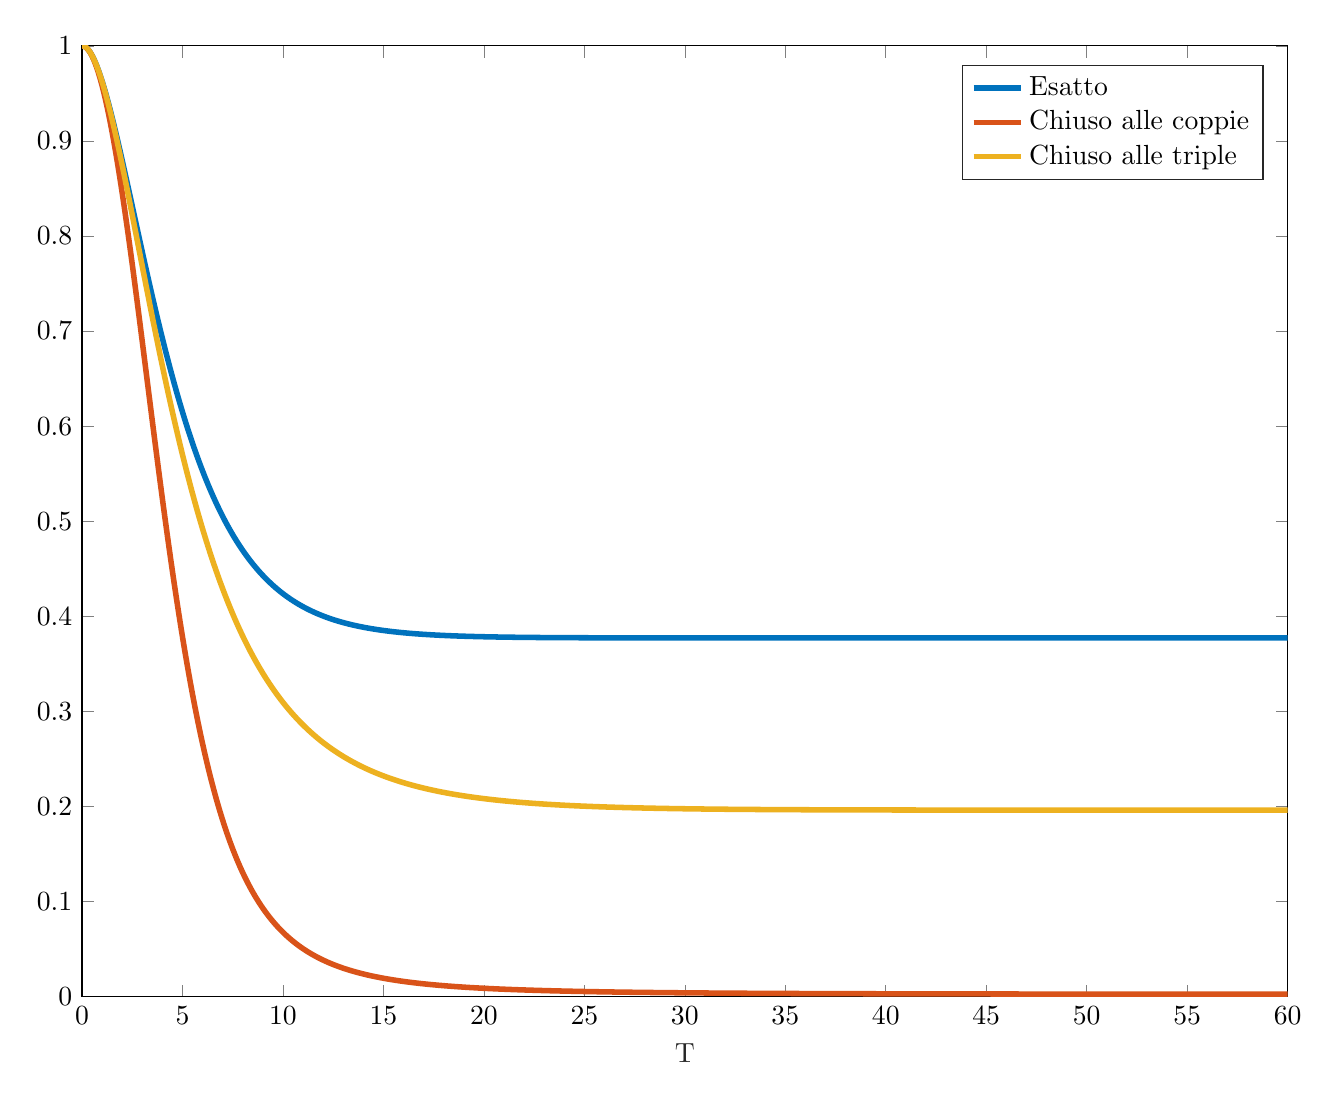
\begin{tikzpicture}

\begin{axis}[%
width=6.028in,
height=4.754in,
at={(1.011in,0.642in)},
scale only axis,
xmin=0,
xmax=60,
xlabel style={font=\color{white!15!black}},
xlabel={T},
ymin=0,
ymax=1,
axis background/.style={fill=white},
legend style={legend cell align=left, align=left, draw=white!15!black}
]
\addplot [color=mycolor1, line width=2.0pt]
  table[row sep=crcr]{%
0	1\\
0.00199053585276749	0.999999821758676\\
0.00398107170553497	0.999999287271421\\
0.00597160755830246	0.999998396893465\\
0.00796214341106994	0.999997150980244\\
0.0123567669950473	0.999993143127503\\
0.0167513905790247	0.999987407889193\\
0.0211460141630021	0.999979949100751\\
0.0255406377469794	0.999970770602233\\
0.0299388563931551	0.999959866624705\\
0.0343370750393307	0.999947247832013\\
0.0387352936855064	0.999932918087308\\
0.043133512331682	0.99991688125802\\
0.0475471725191068	0.999899075937191\\
0.0519608327065316	0.999879559339978\\
0.0563744928939564	0.999858335387465\\
0.0607881530813811	0.999835408004732\\
0.0652173199794049	0.999810691606778\\
0.0696464868774286	0.999784267719513\\
0.0740756537754524	0.999756140321436\\
0.0785048206734761	0.999726313394756\\
0.0829496187548012	0.999694676680182\\
0.0873944168361263	0.999661336466181\\
0.0918392149174515	0.999626296788303\\
0.0962840129987766	0.999589561685518\\
0.100744568101794	0.999550995972635\\
0.105205123204811	0.999510730952902\\
0.109665678307829	0.999468770718551\\
0.114126233410846	0.999425119364942\\
0.118602673075784	0.999379616525619\\
0.123079112740721	0.999332418774366\\
0.127555552405659	0.999283530259728\\
0.132031992070596	0.999232955133084\\
0.136524445545197	0.999180507589601\\
0.141016899019798	0.999126369731132\\
0.1455093524944	0.999070545762162\\
0.150001805969001	0.999013039889722\\
0.154510404254387	0.998953640611314\\
0.159019002539772	0.998892555816567\\
0.163527600825158	0.998829789765537\\
0.168036199110544	0.998765346720531\\
0.172561074936287	0.998698989220849\\
0.17708595076203	0.998630951204912\\
0.181610826587773	0.998561236987975\\
0.186135702413515	0.998489850887247\\
0.190676990405524	0.998416529219182\\
0.195218278397533	0.998341532236025\\
0.199759566389542	0.998264864307858\\
0.204300854381551	0.99818652980642\\
0.208858690959197	0.998106238560546\\
0.213416527536843	0.998024277401581\\
0.217974364114488	0.997940650754059\\
0.222532200692134	0.997855363043875\\
0.227106724202768	0.997768097343535\\
0.231681247713401	0.997679167332637\\
0.236255771224035	0.997588577489792\\
0.240830294734669	0.997496332294675\\
0.245421645441331	0.997402087793233\\
0.250012996147992	0.997306184784038\\
0.254604346854654	0.997208627799406\\
0.259195697561315	0.997109421372416\\
0.263804017673384	0.99700819424998\\
0.268412337785452	0.99690531462263\\
0.273020657897521	0.99680078707601\\
0.27762897800959	0.996694616196225\\
0.282254411746462	0.996586403155648\\
0.286879845483334	0.996476543812783\\
0.291505279220206	0.996365042806223\\
0.296130712957079	0.996251904774722\\
0.300773406613671	0.996136703037344\\
0.305416100270264	0.996019861399835\\
0.310058793926856	0.995901384553362\\
0.314701487583449	0.995781277188947\\
0.319361589521735	0.995659084492062\\
0.324021691460022	0.995535258496532\\
0.328681793398309	0.995409803945715\\
0.333341895336596	0.995282725582526\\
0.338019556071109	0.995153540174664\\
0.342697216805623	0.995022728268747\\
0.347374877540136	0.994890294659947\\
0.35205253827465	0.994756244142687\\
0.356747910447269	0.994620064781757\\
0.361443282619888	0.994482265922303\\
0.366138654792507	0.994342852410934\\
0.370834026965126	0.994201829093197\\
0.375547265516765	0.994058655039184\\
0.380260504068404	0.993913868684887\\
0.384973742620042	0.993767474927966\\
0.389686981171681	0.993619478664712\\
0.394418243246227	0.993469309679876\\
0.399149505320772	0.993317535791578\\
0.403880767395317	0.993164161948147\\
0.408612029469863	0.993009193096236\\
0.41336147459102	0.992852029437397\\
0.418110919712177	0.992693268470303\\
0.422860364833334	0.992532915193569\\
0.427609809954491	0.992370974603824\\
0.432377599961091	0.992206817021958\\
0.437145389967691	0.992041069925322\\
0.44191317997429	0.991873738362433\\
0.44668096998089	0.991704827379509\\
0.451467269141767	0.991533677113809\\
0.456253568302644	0.991360945324967\\
0.461039867463521	0.991186637111017\\
0.465826166624398	0.991010757567379\\
0.47063114173014	0.990832616339664\\
0.475436116835881	0.990652901778434\\
0.480241091941623	0.990471619030852\\
0.485046067047365	0.990288773241155\\
0.489869887370685	0.99010364325504\\
0.494693707694006	0.989916948322967\\
0.499517528017326	0.989728693640843\\
0.504341348340647	0.989538884401329\\
0.509184185682064	0.989346768338733\\
0.51402702302348	0.989153095915621\\
0.518869860364897	0.988957872376255\\
0.523712697706314	0.988761102961329\\
0.528574726619363	0.988562003971675\\
0.533436755532412	0.988361357404694\\
0.53829878444546	0.988159168552612\\
0.543160813358509	0.98795544270377\\
0.548042211039569	0.987749364406118\\
0.55292360872063	0.987541747512065\\
0.55780500640169	0.987332597361411\\
0.56268640408275	0.987121919289747\\
0.56758735048985	0.986908865766242\\
0.572488296896949	0.986694282824967\\
0.577389243304049	0.986478175852903\\
0.582290189711149	0.986260550232503\\
0.587210867601438	0.986040526025034\\
0.592131545491728	0.985818981776135\\
0.597052223382018	0.985595922919578\\
0.601972901272307	0.985371354884277\\
0.606913496388328	0.985144364984483\\
0.611854091504349	0.984915864617257\\
0.61679468662037	0.984685859262764\\
0.621735281736391	0.984454354395988\\
0.626695982628195	0.984220404251613\\
0.631656683519999	0.983984953411577\\
0.636617384411802	0.983748007402045\\
0.641578085303606	0.983509571743672\\
0.646559083672327	0.98326866724142\\
0.651540082041047	0.983026272013021\\
0.656521080409768	0.982782391630246\\
0.661502078778488	0.982537031659021\\
0.666503569383853	0.98228917912712\\
0.671505059989219	0.982039846036422\\
0.676506550594584	0.981789038003902\\
0.68150804119995	0.981536760640362\\
0.686530221876942	0.981281966846773\\
0.691552402553934	0.981025702859716\\
0.696574583230927	0.980767974340972\\
0.701596763907919	0.980508786945815\\
0.706639835866396	0.98024705908213\\
0.711682907824873	0.979983871588318\\
0.71672597978335	0.979719230170567\\
0.721769051741827	0.979453140528221\\
0.72683321952555	0.979184486210138\\
0.731897387309272	0.978914383023414\\
0.736961555092995	0.97864283671824\\
0.742025722876718	0.978369853037629\\
0.747111194287107	0.978094280308223\\
0.752196665697496	0.977817269670045\\
0.757282137107885	0.97753882691689\\
0.762367608518274	0.977258957835032\\
0.767474594900923	0.976976475148993\\
0.772581581283573	0.976692565712589\\
0.777688567666222	0.976407235362809\\
0.782795554048871	0.976120489928786\\
0.78792427039055	0.975831106146045\\
0.793052986732229	0.975540306970049\\
0.798181703073909	0.975248098280582\\
0.803310419415588	0.974954485949224\\
0.808461084325784	0.974658210335209\\
0.81361174923598	0.974360530884015\\
0.818762414146177	0.974061453517812\\
0.823913079056373	0.97376098415022\\
0.82908591482452	0.973457826372435\\
0.834258750592667	0.973153276512815\\
0.839431586360813	0.972847340535507\\
0.84460442212896	0.97254002439576\\
0.849799655005291	0.97222999450725\\
0.854994887881621	0.971918584491747\\
0.860190120757951	0.971605800354966\\
0.865385353634282	0.971291648093377\\
0.870603213699137	0.970974756540108\\
0.875821073763992	0.970656497014573\\
0.881038933828848	0.970336875563643\\
0.886256793893703	0.970015898224591\\
0.891497515445601	0.969692155822238\\
0.896738236997499	0.969367057802491\\
0.901978958549397	0.969040610252967\\
0.907219680101295	0.968712819251329\\
0.912483501408722	0.968382237200377\\
0.917747322716149	0.968050312087533\\
0.923011144023576	0.967717050040742\\
0.928274965331004	0.967382457177642\\
0.933562128954513	0.967045047044285\\
0.938849292578023	0.966706306605565\\
0.944136456201532	0.966366242029344\\
0.949423619825042	0.966024859472814\\
0.954734372782572	0.965680633178794\\
0.960045125740102	0.965335089537381\\
0.965355878697632	0.964988234755934\\
0.970666631655162	0.964640075030783\\
0.976001225418392	0.964289044854154\\
0.981335819181621	0.963936710490052\\
0.98667041294485	0.963583078184914\\
0.99200500670808	0.963228154173783\\
0.997363697280812	0.962870332745004\\
1.00272238785355	0.962511220491182\\
1.00808107842628	0.962150823697415\\
1.01343976899901	0.961789148637038\\
1.0188228172289	0.961424548919564\\
1.02420586545878	0.961058671942506\\
1.02958891368867	0.960691524029197\\
1.03497196191855	0.960323111490839\\
1.04037963341625	0.959951746787766\\
1.04578730491395	0.959579118594248\\
1.05119497641164	0.959205233271429\\
1.05660264790934	0.958830097167953\\
1.06203521338424	0.958451981100932\\
1.06746777885913	0.958072615516885\\
1.07290034433402	0.957692006814344\\
1.07833290980891	0.957310161378968\\
1.08379064506731	0.956925307889959\\
1.08924838032571	0.956539219062339\\
1.09470611558411	0.956151901331599\\
1.10016385084252	0.955763361119982\\
1.1056470369148	0.955371784464716\\
1.11113022298707	0.954978986855011\\
1.11661340905935	0.95458497476289\\
1.12209659513163	0.954189754646746\\
1.12760551858231	0.953791469375167\\
1.13311444203298	0.953391977739819\\
1.13862336548365	0.952991286248824\\
1.14413228893432	0.952589401396296\\
1.14966724184116	0.952184422356571\\
1.15520219474799	0.951778251751113\\
1.16073714765482	0.951370896123712\\
1.16627210056166	0.950962362003764\\
1.17183338076584	0.950550704327301\\
1.17739466097002	0.950137870091388\\
1.18295594117419	0.949723865875048\\
1.18851722137837	0.949308698242523\\
1.19410513262804	0.948890377336704\\
1.19969304387772	0.948470895086909\\
1.20528095512739	0.948050258106961\\
1.21086886637706	0.947628472995503\\
1.21648371859449	0.947203504527376\\
1.22209857081192	0.946777390140901\\
1.22771342302936	0.946350136484262\\
1.23332827524679	0.945921750190066\\
1.23897038457538	0.945490150086655\\
1.24461249390397	0.94505741970176\\
1.25025460323256	0.944623565717482\\
1.25589671256115	0.94418859479995\\
1.26156640151281	0.943750379241692\\
1.26723609046446	0.9433110492512\\
1.27290577941612	0.942870611544051\\
1.27857546836778	0.94242907281945\\
1.28427306633634	0.941984258205439\\
1.28997066430491	0.941538345221924\\
1.29566826227347	0.941091340617517\\
1.30136586024204	0.940643251124048\\
1.30709170327692	0.940191854094465\\
1.31281754631181	0.939739374972921\\
1.31854338934669	0.939285820540611\\
1.32426923238158	0.938831197561545\\
1.33002366371043	0.93837323496267\\
1.33577809503928	0.937914206765464\\
1.34153252636813	0.937454119783261\\
1.34728695769699	0.936992980811795\\
1.35307032782915	0.936528469693615\\
1.35885369796131	0.936062909688224\\
1.36463706809348	0.93559630764064\\
1.37042043822564	0.935128670377867\\
1.37622881553645	0.934657975984608\\
1.38203719284726	0.934186251151717\\
1.38784557015807	0.933713502740253\\
1.39365394746888	0.933239737592897\\
1.39948194569202	0.932763357022515\\
1.40530994391516	0.932285966581078\\
1.41113794213829	0.931807573125033\\
1.41696594036143	0.931328183492157\\
1.4228137248248	0.930846171922117\\
1.42866150928816	0.93036317113504\\
1.43450929375153	0.929879187981882\\
1.44035707821489	0.929394229294635\\
1.44622478964653	0.928906644386903\\
1.45209250107816	0.928418091008538\\
1.45796021250979	0.927928576004031\\
1.46382792394143	0.927438106198621\\
1.46971570462452	0.926945005989889\\
1.4756034853076	0.926450958146903\\
1.48149126599069	0.92595596950672\\
1.48737904667378	0.925460046886862\\
1.49328704060906	0.92496148976845\\
1.49919503454433	0.924462005939698\\
1.50510302847961	0.923961602229264\\
1.51101102241489	0.923460285445991\\
1.51693937480906	0.922956330200663\\
1.52286772720322	0.922451469254184\\
1.52879607959739	0.92194570942585\\
1.53472443199155	0.921439057514862\\
1.540673290528	0.920929763202963\\
1.54662214906446	0.920419584281743\\
1.55257100760091	0.919908527560182\\
1.55851986613736	0.919396599826883\\
1.56448937947106	0.918882025907562\\
1.57045889280476	0.918366588551248\\
1.57642840613847	0.917850294555645\\
1.58239791947216	0.917333150697808\\
1.58838823791446	0.916813356965575\\
1.59437855635675	0.91629272104683\\
1.60036887479904	0.915771249727046\\
1.60635919324133	0.915248949770777\\
1.61237046959671	0.914723996276508\\
1.61838174595208	0.914198221921806\\
1.62439302230746	0.913671633478967\\
1.63040429866284	0.913144237699094\\
1.63643668672632	0.912614184874215\\
1.6424690747898	0.912083332588474\\
1.64850146285328	0.911551687600037\\
1.65453385091676	0.911019256645617\\
1.66058750665404	0.91048416519403\\
1.66664116239132	0.909948295752224\\
1.67269481812859	0.909411655063294\\
1.67874847386587	0.908874249848617\\
1.68482355500326	0.908334180776516\\
1.69089863614064	0.907793355253629\\
1.69697371727803	0.907251780007037\\
1.70304879841541	0.906709461741846\\
1.70914546464501	0.90616447633396\\
1.71524213087462	0.905618756081198\\
1.72133879710422	0.905072307693691\\
1.72743546333383	0.904525137859335\\
1.73355387572031	0.903975297726557\\
1.73967228810678	0.903424744419141\\
1.74579070049326	0.902873484629328\\
1.75190911287974	0.902321525026872\\
1.75804943463327	0.901766892032233\\
1.76418975638681	0.901211567595199\\
1.77033007814035	0.900655558389186\\
1.77647039989388	0.900098871064876\\
1.78263279664118	0.899539507293123\\
1.78879519338848	0.89897947387087\\
1.79495759013578	0.898418777451781\\
1.80111998688309	0.897857424666537\\
1.80730462566597	0.897293392509363\\
1.81348926444885	0.896728712551132\\
1.81967390323173	0.896163391424825\\
1.82585854201462	0.8955974357402\\
1.83206559217232	0.895028797811561\\
1.83827264233002	0.89445953398657\\
1.84447969248772	0.893889650876606\\
1.85068674264543	0.893319155069578\\
1.85691637550678	0.892745974228531\\
1.86314600836813	0.892172189448912\\
1.86937564122948	0.891597807319571\\
1.87560527409083	0.891022834405649\\
1.88185766319929	0.890445173730886\\
1.88811005230775	0.889866931126185\\
1.89436244141622	0.889288113156949\\
1.90061483052468	0.888708726364638\\
1.90689015093446	0.888126649214895\\
1.91316547134424	0.88754401219264\\
1.91944079175402	0.886960821838908\\
1.92571611216381	0.886377084670562\\
1.93201454150218	0.885790654582199\\
1.93831297084055	0.88520368672529\\
1.94461140017892	0.884616187615593\\
1.9509098295173	0.884028163744458\\
1.95723154808653	0.883437444416735\\
1.96355326665576	0.882846209468748\\
1.96987498522499	0.882254465390062\\
1.97619670379422	0.881662218645611\\
1.98254189319299	0.881067274064932\\
1.98888708259176	0.880471836054604\\
1.99523227199053	0.87987591107709\\
2.0015774613893	0.879279505569999\\
2.00794630624256	0.878680399844427\\
2.01431515109582	0.878080822919909\\
2.02068399594908	0.877480781230901\\
2.02705284080234	0.876880281186783\\
2.03344552746868	0.876277078662849\\
2.03983821413503	0.875673427208743\\
2.04623090080137	0.875069333230006\\
2.05262358746771	0.874464803106888\\
2.05904030495676	0.873857568279661\\
2.06545702244581	0.873249906826964\\
2.07187373993486	0.872641825124522\\
2.07829045742391	0.872033329522558\\
2.084731396657	0.871422127101608\\
2.0911723358901	0.870810520393801\\
2.0976132751232	0.870198515744148\\
2.1040542143563	0.869586119471944\\
2.11051956957009	0.868971014244709\\
2.11698492478388	0.868355527100966\\
2.12345027999767	0.86773966435411\\
2.12991563521146	0.867123432291618\\
2.13640560238783	0.866504489268607\\
2.1428955695642	0.86588518672921\\
2.14938553674057	0.865265530954317\\
2.15587550391694	0.864645528198689\\
2.16239028199053	0.864022812495508\\
2.16890506006412	0.863399759703756\\
2.17541983813771	0.86277637607092\\
2.1819346162113	0.86215266781816\\
2.18847440630977	0.861526244724612\\
2.19501419640825	0.860899506996016\\
2.20155398650673	0.86027246084557\\
2.20809377660521	0.859645112459944\\
2.21465878275268	0.859015047369792\\
2.22122378890015	0.858384690121795\\
2.22778879504762	0.857754046893969\\
2.23435380119508	0.857123123837612\\
2.24094422983074	0.856489482291673\\
2.24753465846639	0.855855571086803\\
2.25412508710205	0.85522139636495\\
2.2607155157377	0.854586964241152\\
2.2673315759421	0.853949811902932\\
2.27394763614649	0.853312412424431\\
2.28056369635089	0.852674771910644\\
2.28717975655528	0.852036896439472\\
2.29382166035897	0.851396299062792\\
2.30046356416266	0.850755477082241\\
2.30710546796636	0.850114436564983\\
2.31374737177005	0.849473183550898\\
2.32041533418655	0.848829206974096\\
2.32708329660306	0.848185028345644\\
2.33375125901957	0.84754065369399\\
2.34041922143607	0.846896089020119\\
2.34711345989709	0.846248799218266\\
2.3538076983581	0.845601329930892\\
2.36050193681912	0.84495368714685\\
2.36719617528013	0.844305876827357\\
2.37391691043736	0.843655339832736\\
2.3806376455946	0.843004645930697\\
2.38735838075183	0.842353801069629\\
2.39407911590907	0.841702811170099\\
2.40082657131283	0.841049093101204\\
2.40757402671659	0.840395240713082\\
2.41432148212035	0.839741259912775\\
2.42106893752412	0.839087156579339\\
2.42784333963791	0.838430323637689\\
2.4346177417517	0.837773378973211\\
2.4413921438655	0.837116328450731\\
2.44816654597929	0.836459177906918\\
2.4549681243632	0.835799296357661\\
2.4617697027471	0.835139325688318\\
2.46857128113101	0.834479271720627\\
2.47537285951492	0.833819140248002\\
2.48220184698832	0.833156276402645\\
2.48903083446173	0.832493346044435\\
2.49585982193513	0.831830354951152\\
2.50268880940853	0.831167308872091\\
2.50954544177924	0.830501529113496\\
2.51640207414995	0.829835705451944\\
2.52325870652066	0.829169843620389\\
2.53011533889137	0.828503949323143\\
2.53699985562036	0.827835320039893\\
2.54388437234935	0.827166669464428\\
2.55076888907833	0.826498003284008\\
2.55765340580732	0.825829327157098\\
2.5645660494942	0.825157914792538\\
2.57147869318108	0.824486503745555\\
2.57839133686796	0.823815099656852\\
2.58530398055484	0.823143708138183\\
2.59224499685821	0.822469579197461\\
2.59918601316159	0.821795474181377\\
2.60612702946496	0.821121398683211\\
2.61306804576833	0.820447358267151\\
2.62003768421203	0.819770579238379\\
2.62700732265572	0.819093846736811\\
2.63397696109942	0.818417166307444\\
2.64094659954311	0.817740543466038\\
2.64794511298781	0.817061180871296\\
2.65494362643251	0.816381887400082\\
2.6619421398772	0.815702668548248\\
2.6689406533219	0.815023529782269\\
2.67596829852112	0.814341650123513\\
2.68299594372033	0.813659862176647\\
2.69002358891955	0.812978171387516\\
2.69705123411877	0.812296583172455\\
2.70410827073433	0.811612253027156\\
2.71116530734989	0.810928037172412\\
2.71822234396545	0.810243941003205\\
2.72527938058101	0.809559969884872\\
2.73236607296869	0.808873255733056\\
2.73945276535637	0.8081866784391\\
2.74653945774405	0.807500243346265\\
2.75362615013173	0.806813955768036\\
2.76074276611797	0.80612492411157\\
2.76785938210422	0.805436051867224\\
2.77497599809046	0.804747344325684\\
2.78209261407671	0.80405880674773\\
2.78923942490227	0.803367524116398\\
2.79638623572783	0.802676423436726\\
2.80353304655339	0.801985509945964\\
2.81067985737896	0.801294788851337\\
2.81785713902212	0.800601321675728\\
2.82503442066529	0.799908058974995\\
2.83221170230846	0.799215005932098\\
2.83938898395163	0.798522167699853\\
2.84659701614953	0.797826582407408\\
2.85380504834743	0.797131224095098\\
2.86101308054533	0.796436097890741\\
2.86822111274323	0.795741208891892\\
2.87546017926332	0.795043571882027\\
2.88269924578341	0.794346184337994\\
2.88993831230351	0.793649051331612\\
2.8971773788236	0.792952177904329\\
2.90444776780364	0.792252555517335\\
2.91171815678368	0.791553205060737\\
2.91898854576373	0.790854131549502\\
2.92625893474377	0.79015533996812\\
2.93356093845992	0.789453798509476\\
2.94086294217606	0.788752551423082\\
2.94816494589221	0.788051603666203\\
2.95546694960836	0.78735096016552\\
2.96280086487659	0.786647565869443\\
2.97013478014483	0.785944488363232\\
2.97746869541306	0.785241732545591\\
2.9848026106813	0.784539303284548\\
2.99216873909201	0.783834122294099\\
2.99953486750271	0.783129280485392\\
3.00690099591342	0.782424782697724\\
3.01426712432413	0.781720633739616\\
3.02166577186631	0.781013732145562\\
3.02906441940849	0.780307192097875\\
3.03646306695067	0.77960101837559\\
3.04386171449286	0.778895215726875\\
3.05129319192691	0.778186659534979\\
3.05872466936097	0.77747848722535\\
3.06615614679503	0.776770703515908\\
3.07358762422909	0.77606331309362\\
3.08105224696524	0.775353168239552\\
3.0885168697014	0.774643429573451\\
3.09598149243755	0.773934101751273\\
3.1034461151737	0.773225189397932\\
3.11094420406679	0.772513521675254\\
3.11844229295988	0.771802282414669\\
3.12594038185297	0.771091476209312\\
3.13343847074605	0.770381107621199\\
3.14097035080817	0.769667982807694\\
3.14850223087028	0.768955308697318\\
3.1560341109324	0.768243089819536\\
3.16356599099451	0.767531330672614\\
3.17113199342146	0.766816814342122\\
3.17869799584842	0.766102770921441\\
3.18626399827537	0.765389204875508\\
3.19383000070233	0.764676120637992\\
3.20143046110215	0.763960278332976\\
3.20903092150198	0.763244931108624\\
3.21663138190181	0.762530083364495\\
3.22423184230164	0.761815739468807\\
3.2318671021242	0.761098636569872\\
3.23950236194676	0.76038205088534\\
3.24713762176933	0.759665986748535\\
3.25477288159189	0.758950448461375\\
3.26244328804483	0.758232150200888\\
3.27011369449776	0.757514391250146\\
3.2777841009507	0.756797175875381\\
3.28545450740363	0.75608050831136\\
3.29316041266953	0.75536107985237\\
3.30086631793543	0.754642212758681\\
3.30857222320133	0.753923911228576\\
3.31627812846722	0.753206179428818\\
3.32401989110489	0.752485685739595\\
3.33176165374256	0.751765775430258\\
3.33950341638023	0.751046452630283\\
3.3472451790179	0.750327721437575\\
3.35502316313618	0.749606227375318\\
3.36280114725446	0.748885338665266\\
3.37057913137275	0.748165059367225\\
3.37835711549103	0.747445393509386\\
3.38617169154667	0.746722963752538\\
3.3939862676023	0.746001161276769\\
3.40180084365794	0.745279990071358\\
3.40961541971357	0.744559454093924\\
3.41746696420648	0.743836153177668\\
3.42531850869938	0.743113501426706\\
3.43317005319229	0.742391502758927\\
3.4410215976852	0.741670161060521\\
3.44891049346576	0.740946053355703\\
3.45679938924632	0.740222616654573\\
3.46468828502688	0.739499854802762\\
3.47257718080744	0.73877777161417\\
3.48050381756295	0.738052921290614\\
3.48843045431847	0.737328763762236\\
3.49635709107398	0.736605302801542\\
3.50428372782949	0.73588254214928\\
3.51224850159594	0.735157013229016\\
3.52021327536239	0.734432198847353\\
3.52817804912884	0.733708102702804\\
3.53614282289529	0.732984728462101\\
3.54414613607264	0.732258584826045\\
3.55214944924998	0.731533177422781\\
3.56015276242733	0.730808509875957\\
3.56815607560468	0.730084585777418\\
3.57619833889781	0.729357890998277\\
3.58424060219095	0.728631954096074\\
3.59228286548408	0.727906778618717\\
3.60032512877721	0.727182368082297\\
3.60840675922679	0.726455185613617\\
3.61648838967638	0.725728782614804\\
3.62457002012596	0.72500316255715\\
3.63265165057554	0.724278328880116\\
3.64077307248204	0.723550721981961\\
3.64889449438855	0.722823916094374\\
3.65701591629505	0.722097914611151\\
3.66513733820155	0.721372720894247\\
3.67329898353354	0.720644752607071\\
3.68146062886554	0.719917606818002\\
3.68962227419754	0.719191286842452\\
3.69778391952953	0.718465795963995\\
3.70598622860803	0.717737529059123\\
3.71418853768653	0.717010106085933\\
3.72239084676502	0.716283530280568\\
3.73059315584352	0.715557804847335\\
3.73883657626523	0.714829301934817\\
3.74707999668693	0.714101664332568\\
3.75532341710863	0.71337489519657\\
3.76356683753034	0.712648997650976\\
3.77185182516863	0.711920321102255\\
3.78013681280692	0.711192531186569\\
3.78842180044522	0.710465630978843\\
3.79670678808351	0.709739623522185\\
3.80503380745825	0.709010835450583\\
3.81336082683299	0.708282955278201\\
3.82168784620774	0.707555985998004\\
3.83001486558248	0.70682993057116\\
3.83838438958511	0.706101092869558\\
3.84675391358775	0.705373184275945\\
3.85512343759039	0.704646207700424\\
3.86349296159302	0.703920166021322\\
3.8719054722877	0.703191340306052\\
3.88031798298237	0.702463464849459\\
3.88873049367705	0.701736542477872\\
3.89714300437172	0.701010575985873\\
3.90559899284027	0.700281823625211\\
3.91405498130882	0.699554042615114\\
3.92251096977737	0.698827235697222\\
3.93096695824593	0.698101405581464\\
3.93946692479213	0.697372787693018\\
3.94796689133833	0.696645162187539\\
3.95646685788454	0.695918531721059\\
3.96496682443074	0.695192898917933\\
3.97351127881372	0.694464476364191\\
3.98205573319669	0.693737067165678\\
3.99060018757967	0.693010673891889\\
3.99914464196265	0.692285299080687\\
4.00773410425464	0.691557132412381\\
4.01632356654662	0.690830000010957\\
4.02491302883861	0.690103904358436\\
4.0335024911306	0.689378847905262\\
4.04213749081375	0.688650997455598\\
4.05077249049689	0.687924202123145\\
4.05940749018004	0.687198464301517\\
4.06804248986318	0.686473786352797\\
4.07672356764034	0.685746312101832\\
4.08540464541749	0.685019913756793\\
4.09408572319465	0.684294593621931\\
4.10276680097181	0.683570353970033\\
4.11149450824228	0.682843315608809\\
4.12022221551276	0.682117373880159\\
4.12894992278323	0.681392530998021\\
4.1376776300537	0.680668789144934\\
4.14645252883691	0.679942246101057\\
4.15522742762012	0.67921682035384\\
4.16400232640333	0.678492514025946\\
4.17277722518654	0.677769329208709\\
4.18159988926615	0.677043340571352\\
4.19042255334575	0.676318489831943\\
4.19924521742536	0.675594779020892\\
4.20806788150496	0.674872210137363\\
4.21693889629988	0.674146834689816\\
4.22580991109479	0.673422617678393\\
4.23468092588971	0.672699561040279\\
4.24355194068463	0.671977666681489\\
4.2524719033702	0.671252962913006\\
4.26139186605577	0.670529438055408\\
4.27031182874135	0.669807093951656\\
4.27923179142692	0.669085932413638\\
4.28820131218307	0.668361958440768\\
4.29717083293922	0.667639183790098\\
4.30614035369538	0.66691761020937\\
4.31510987445153	0.666197239415347\\
4.32412957614907	0.665474053032334\\
4.33314927784661	0.664752086319247\\
4.34216897954416	0.664031340927597\\
4.3511886812417	0.663311818478019\\
4.36025919971018	0.662589477159914\\
4.36932971817866	0.66186837579575\\
4.37840023664715	0.661148515939786\\
4.38747075511563	0.660429899115513\\
4.39659274002011	0.659708459973978\\
4.40571472492458	0.658988281006755\\
4.41483670982906	0.658269363669818\\
4.42395869473353	0.657551709388486\\
4.43313280988389	0.656831229174936\\
4.44230692503424	0.656112029292527\\
4.45148104018459	0.655394111097902\\
4.46065515533495	0.65467747591717\\
4.469882079136	0.653958011015916\\
4.47910900293706	0.653239846539261\\
4.48833592673811	0.652522983743459\\
4.49756285053916	0.651807423854356\\
4.50684327607396	0.651089030305535\\
4.51612370160877	0.650371957211537\\
4.52540412714357	0.649656205727151\\
4.53468455267837	0.648941776976898\\
4.54401918924822	0.648224510387736\\
4.55335382581807	0.647508584220893\\
4.56268846238792	0.64679399952861\\
4.57202309895777	0.646080757333\\
4.58141267108196	0.645364672987779\\
4.59080224320616	0.644649948969802\\
4.60019181533036	0.64393658622766\\
4.60958138745456	0.643224585679965\\
4.61902663678989	0.64250973842562\\
4.62847188612523	0.641796271341509\\
4.63791713546056	0.641084185271456\\
4.6473623847959	0.640373481029459\\
4.65686406984621	0.639659925333481\\
4.66636575489653	0.63894776958927\\
4.67586743994685	0.638237014534747\\
4.68536912499717	0.63752766087817\\
4.69492802222378	0.636815450781042\\
4.7044869194504	0.636104660356477\\
4.71404581667701	0.63539529023534\\
4.72360471390363	0.634687341019005\\
4.73320764525141	0.633977561870957\\
4.74281057659919	0.633269217875996\\
4.75241350794698	0.632562309554549\\
4.76201643929476	0.631856837397901\\
4.77165794452804	0.631149976734965\\
4.78129944976131	0.630444564701867\\
4.79094095499459	0.629740601707782\\
4.80058246022786	0.629038088133163\\
4.81026314694842	0.628334178280334\\
4.81994383366897	0.627631730332827\\
4.82962452038952	0.626930744588973\\
4.83930520711008	0.62623122131881\\
4.84902565638322	0.62553029655961\\
4.85874610565637	0.624830846772498\\
4.86846655492951	0.624132872145348\\
4.87818700420266	0.623436372838168\\
4.88794780523678	0.622738466858853\\
4.89770860627089	0.622042048712455\\
4.90746940730501	0.621347118476764\\
4.91723020833913	0.620653676202129\\
4.92703195872998	0.61995882209936\\
4.93683370912084	0.61926546848714\\
4.9466354595117	0.618573615333522\\
4.95643720990256	0.617883262579554\\
4.96628051524823	0.617191492912535\\
4.97612382059389	0.616501236192984\\
4.98596712593956	0.615812492279559\\
4.99581043128522	0.615125261004338\\
5.00569590732134	0.614436607669498\\
5.01558138335745	0.613749479541357\\
5.02546685939356	0.613063876369493\\
5.03535233542967	0.612379797877338\\
5.04528060635073	0.611694292253313\\
5.05520887727179	0.611010323899909\\
5.06513714819285	0.610327892457923\\
5.07506541911391	0.609646997542444\\
5.08503711889176	0.608964670423353\\
5.0950088186696	0.60828389244615\\
5.10498051844744	0.607604663143138\\
5.11495221822528	0.606926982021347\\
5.12496799094167	0.606247863621065\\
5.13498376365806	0.605570306043919\\
5.14499953637444	0.604894308713983\\
5.15501530909083	0.604219871030501\\
5.16507580953502	0.603543990969745\\
5.17513630997921	0.602869683226047\\
5.18519681042339	0.602196947115499\\
5.19525731086758	0.601525781929807\\
5.2053632039849	0.600853169301178\\
5.21546909710223	0.600182140298586\\
5.22557499021955	0.599512694130377\\
5.23568088333688	0.598844829980956\\
5.24583284576096	0.598175513274013\\
5.25598480818505	0.597507791319883\\
5.26613677060914	0.596841663219378\\
5.27628873303322	0.596177128049819\\
5.28648745229033	0.595511135233062\\
5.29668617154743	0.594846748116043\\
5.30688489080453	0.594183965692236\\
5.31708361006163	0.593522786932075\\
5.32732978639303	0.592860145362116\\
5.33757596272443	0.592199120261753\\
5.34782213905582	0.591539710517307\\
5.35806831538722	0.590881914992505\\
5.36836266133408	0.590222651472515\\
5.37865700728095	0.58956501501744\\
5.38895135322782	0.588909004406602\\
5.39924569917468	0.588254618397192\\
5.40958894010065	0.587598759173677\\
5.41993218102661	0.586944537438397\\
5.43027542195257	0.586291951863823\\
5.44061866287853	0.585641001100749\\
5.45101153706255	0.584988571888487\\
5.46140441124658	0.584337790418214\\
5.4717972854306	0.583688655255672\\
5.48219015961463	0.583041164945389\\
5.49263341945276	0.582392190883131\\
5.50307667929089	0.581744874649714\\
5.51351993912902	0.581099214704257\\
5.52396319896715	0.580455209485132\\
5.53445761187213	0.579809715113641\\
5.54495202477712	0.579165888493741\\
5.5554464376821	0.578523727978016\\
5.56594085058709	0.57788323189877\\
5.57648719831941	0.577241241236843\\
5.58703354605173	0.576600928087592\\
5.59757989378405	0.57596229069713\\
5.60812624151637	0.575325327291767\\
5.61872532103302	0.574686863817564\\
5.62932440054967	0.574050087458003\\
5.63992348006633	0.573414996352777\\
5.65052255958298	0.572781588622248\\
5.66117518401188	0.572146675249526\\
5.67182780844078	0.571513458436991\\
5.68248043286967	0.570881936217939\\
5.69313305729857	0.57025210660682\\
5.70384005671797	0.569620765675478\\
5.71454705613736	0.568991130596223\\
5.72525405555675	0.568363199295964\\
5.73596105497615	0.567736969683245\\
5.74672327665992	0.567109222983043\\
5.75748549834369	0.566483191275873\\
5.76824772002746	0.565858872382238\\
5.77900994171123	0.565236264104768\\
5.78982825023888	0.56461213290684\\
5.80064655876654	0.563989725694474\\
5.81146486729419	0.563369040181737\\
5.82228317582184	0.56275007406531\\
5.83315845473553	0.562129579064966\\
5.84403373364921	0.561510816897198\\
5.8549090125629	0.560893785169574\\
5.86578429147658	0.560278481472775\\
5.87671744355088	0.559661642815785\\
5.88765059562518	0.559046545695661\\
5.89858374769948	0.558433187613387\\
5.90951689977378	0.557821566053567\\
5.92050884813521	0.557208403315094\\
5.93150079649664	0.556596990678004\\
5.94249274485807	0.555987325536595\\
5.9534846932195	0.555379405269292\\
5.96453638108293	0.554769937512167\\
5.97558806894636	0.554162228283844\\
5.98663975680979	0.553556274871806\\
5.99769144467322	0.55295207454817\\
6.00880383710542	0.552346320268695\\
6.01991622953761	0.551742332811372\\
6.0310286219698	0.551140109356709\\
6.042141014402	0.550539647070371\\
6.05331509935885	0.549937624188749\\
6.0644891843157	0.549337376291699\\
6.07566326927256	0.548738900452576\\
6.08683735422941	0.548142193730413\\
6.09807414230094	0.547543919652601\\
6.10931093037248	0.546947428593692\\
6.12054771844401	0.54635271751968\\
6.13178450651555	0.545759783382765\\
6.14308503319571	0.54516527492746\\
6.15438555987588	0.544572557400632\\
6.16568608655605	0.543981627660675\\
6.17698661323621	0.543392482552726\\
6.18835193888863	0.542801756005233\\
6.19971726454106	0.542212828174111\\
6.21108259019348	0.54162569580989\\
6.2224479158459	0.541040355650384\\
6.23387912710053	0.540453426741613\\
6.24531033835517	0.539868304218699\\
6.2567415496098	0.539284984724016\\
6.26817276086443	0.538703464887764\\
6.2796709718506	0.538120348785365\\
6.29116918283678	0.537539046623309\\
6.30266739382295	0.536959554935483\\
6.31416560480912	0.536381870244157\\
6.32573195844141	0.535802581544184\\
6.33729831207371	0.535225114227577\\
6.34886466570601	0.534649464719378\\
6.36043101933831	0.53407562943357\\
6.37206668825559	0.533500182172552\\
6.38370235717287	0.532926563630014\\
6.39533802609016	0.532354770121757\\
6.40697369500744	0.531784797953094\\
6.41867988207414	0.53121320564334\\
6.43038606914084	0.530643449282688\\
6.44209225620754	0.530075525077271\\
6.45379844327423	0.529509429223309\\
6.46557638449348	0.528941704772323\\
6.47735432571273	0.528375823400596\\
6.48913226693197	0.527811781204128\\
6.50091020815122	0.527249574269585\\
6.51276117329228	0.526685730017193\\
6.52461213843333	0.526123735877655\\
6.53646310357439	0.525563587836327\\
6.54831406871544	0.52500528186983\\
6.56023936237899	0.524445329605241\\
6.57216465604253	0.523887234394432\\
6.58408994970607	0.523330992111578\\
6.59601524336962	0.52277659862271\\
6.608016207688	0.522220549527953\\
6.62001717200638	0.521666364339628\\
6.63201813632476	0.521114038820136\\
6.64401910064313	0.520563568724343\\
6.65609711612489	0.520011433410394\\
6.66817513160664	0.519461168771536\\
6.68025314708839	0.518912770457762\\
6.69233116257014	0.51836623411215\\
6.70448764976455	0.517818022619091\\
6.71664413695897	0.517271688490202\\
6.72880062415338	0.51672722726239\\
6.7409571113478	0.516184634466269\\
6.75319353351478	0.515640356222703\\
6.76542995568177	0.51509796195764\\
6.77766637784875	0.514557447094169\\
6.78990280001574	0.514018807049725\\
6.80222066442117	0.513478470899837\\
6.8145385288266	0.512940025272847\\
6.82685639323203	0.512403465477243\\
6.83917425763746	0.511868786816509\\
6.85157511856051	0.511332400975453\\
6.86397597948357	0.510797912137034\\
6.87637684040662	0.510265315494301\\
6.88877770132968	0.509734606235961\\
6.90126316148383	0.509202178321148\\
6.91374862163799	0.508671653829299\\
6.92623408179214	0.508143027837133\\
6.93871954194629	0.507616295417692\\
6.95129125486549	0.507087832441967\\
6.96386296778468	0.506561279255604\\
6.97643468070388	0.506036630818031\\
6.98900639362307	0.505513882085683\\
7.00166606764739	0.504989390390111\\
7.0143257416717	0.504466814802535\\
7.02698541569601	0.503946150164072\\
7.03964508972033	0.503427391313538\\
7.05239448925109	0.502906876622812\\
7.06514388878186	0.502388284316947\\
7.07789328831262	0.501871609117657\\
7.09064268784339	0.501356845745063\\
7.10348363709426	0.500840313123935\\
7.11632458634514	0.500325709129307\\
7.12916553559601	0.499813028362327\\
7.14200648484689	0.499302265423267\\
7.15494087138423	0.498789719251357\\
7.16787525792157	0.49827910791935\\
7.18080964445891	0.497770425906585\\
7.19374403099625	0.497263667692257\\
7.20677380774895	0.496755111707496\\
7.21980358450165	0.496248496754745\\
7.23283336125435	0.495743817190207\\
7.24586313800706	0.495241067370692\\
7.25899032889946	0.494736504577063\\
7.27211751979186	0.494233888994181\\
7.28524471068426	0.493733214853699\\
7.29837190157667	0.493234476388647\\
7.31159860422458	0.492733909090775\\
7.32482530687249	0.492235295177011\\
7.3380520095204	0.491738628752949\\
7.35127871216831	0.491243903926344\\
7.36460710304072	0.490747333677556\\
7.37793549391314	0.490252722989598\\
7.39126388478556	0.489760065840395\\
7.40459227565797	0.489269356210835\\
7.41802461355885	0.488776783836251\\
7.43145695145972	0.488286177211512\\
7.4448892893606	0.487797530185159\\
7.45832162726148	0.487310836609515\\
7.47186025959003	0.486822262136339\\
7.48539889191859	0.486335659624204\\
7.49893752424715	0.485851022790435\\
7.51247615657571	0.485368345356975\\
7.52612352432791	0.484883768006016\\
7.53977089208011	0.484401168859878\\
7.55341825983232	0.483920541502713\\
7.56706562758452	0.483441879524145\\
7.58082427117841	0.482961297684382\\
7.5945829147723	0.482482700336894\\
7.60834155836619	0.482006080930566\\
7.62210020196009	0.481531432920639\\
7.63597276754062	0.481054844121519\\
7.64984533312116	0.48058024615764\\
7.66371789870169	0.480107632340386\\
7.67759046428223	0.479636995988402\\
7.69157971106386	0.479164396852477\\
7.70556895784549	0.478693794963073\\
7.71955820462712	0.478225183491682\\
7.73354745140875	0.477758555617988\\
7.7476562591015	0.477289941829104\\
7.76176506679424	0.476823331780029\\
7.77587387448699	0.476358718499807\\
7.78998268217974	0.475896095026628\\
7.80421406003167	0.475431461263443\\
7.81844543788359	0.474968837830312\\
7.83267681573552	0.474508217611091\\
7.84690819358745	0.47404959349976\\
7.86126528820976	0.473588933431042\\
7.87562238283208	0.473130290395324\\
7.8899794774544	0.472673657128333\\
7.90433657207672	0.472219026376937\\
7.91882267896367	0.471762332558598\\
7.93330878585062	0.471307662606364\\
7.94779489273757	0.470855009104685\\
7.96228099962452	0.470404364650191\\
7.97689957365268	0.469951628483443\\
7.99151814768085	0.46950092316482\\
8.00613672170902	0.469052241124105\\
8.02075529573718	0.46860557480434\\
8.03550996276884	0.468156786485598\\
8.0502646298005	0.46771003616612\\
8.06501929683216	0.467265316117382\\
8.07977396386382	0.466822618625231\\
8.09466853533245	0.466377767035128\\
8.10956310680107	0.465934960786869\\
8.12445767826969	0.465494191989703\\
8.13935224973832	0.465055452768402\\
8.15439073744049	0.464614525391506\\
8.16942922514267	0.464175650914786\\
8.18446771284484	0.463738821281037\\
8.19950620054702	0.463304028449767\\
8.2146928332504	0.46286701127836\\
8.22987946595378	0.462432054807803\\
8.24506609865717	0.461999150809868\\
8.26025273136055	0.461568291074278\\
8.27559197362809	0.461135168490501\\
8.29093121589562	0.460704114679833\\
8.30627045816316	0.460275121238087\\
8.32160970043069	0.45984817978031\\
8.33710627308224	0.459418934439574\\
8.35260284573378	0.458991766247885\\
8.36809941838533	0.458566666619748\\
8.38359599103687	0.458143626990239\\
8.39925489573158	0.457718239643119\\
8.41491380042629	0.457294938160428\\
8.430572705121	0.456873713769555\\
8.44623160981571	0.456454557719853\\
8.46205815432056	0.45603300707726\\
8.4778846988254	0.455613551393215\\
8.49371124333024	0.455196181701677\\
8.50953778783509	0.45478088906002\\
8.52553761739547	0.454363151561061\\
8.54153744695585	0.453947518537597\\
8.55753727651623	0.453533980823271\\
8.57353710607661	0.453122529276662\\
8.58971623619016	0.452708578899319\\
8.60589536630372	0.452296742986082\\
8.62207449641727	0.451887012162765\\
8.63825362653082	0.451479377081701\\
8.65461848330403	0.451069185044318\\
8.67098334007723	0.450661117986446\\
8.68734819685043	0.45025516631783\\
8.70371305362364	0.449851320476401\\
8.72018188980809	0.449447024964282\\
8.73665072599255	0.44904484278108\\
8.75311956217701	0.44864476426797\\
8.76958839836146	0.448246779795427\\
8.78614348346302	0.44784881186571\\
8.80269856856458	0.447452940544318\\
8.81925365366614	0.447059156139355\\
8.83580873876771	0.446667448989204\\
8.85245111606455	0.446275760421291\\
8.86909349336139	0.445886151585106\\
8.88573587065824	0.445498612758064\\
8.90237824795508	0.445113134248816\\
8.91910883699713	0.44472767951133\\
8.93583942603918	0.444344287445115\\
8.95257001508123	0.443962948299487\\
8.96930060412328	0.443583652355937\\
8.98612034063892	0.443204385147709\\
9.00294007715455	0.442827163374544\\
9.01975981367019	0.442451977260208\\
9.03657955018582	0.442078817061574\\
9.05348938408815	0.441705690392902\\
9.07039921799048	0.441334591754774\\
9.08730905189281	0.440965511347931\\
9.10421888579513	0.440598439407135\\
9.12121978296026	0.440231405592988\\
9.13822068012539	0.439866382244268\\
9.15522157729052	0.43950335954118\\
9.17222247445565	0.439142327698849\\
9.18931541587169	0.43878133841151\\
9.20640835728774	0.438422341871222\\
9.22350129870378	0.438065328240113\\
9.24059424011982	0.437710287716112\\
9.25778022278737	0.437355293998296\\
9.27496620545493	0.437002275163282\\
9.29215218812249	0.436651221357545\\
9.30933817079004	0.436302122764234\\
9.32661820779546	0.435953075060338\\
9.34389824480088	0.435605984236357\\
9.3611782818063	0.435260840425508\\
9.37845831881172	0.434917633798537\\
9.39583344002363	0.434574481972762\\
9.41320856123555	0.434233268892603\\
9.43058368244747	0.433893984680378\\
9.44795880365938	0.433556619496775\\
9.46543005570071	0.433219312866007\\
9.48290130774205	0.432883926722187\\
9.50037255978338	0.432550451179066\\
9.51784381182471	0.432218876389586\\
9.53541225878365	0.431887363741213\\
9.55298070574258	0.431557753203786\\
9.57054915270152	0.431230034884782\\
9.58811759966045	0.430904198931681\\
9.60578432346384	0.430578428548395\\
9.62345104726722	0.430254541789656\\
9.64111777107061	0.42993252875893\\
9.658784494874	0.429612379600483\\
9.67655059520445	0.429292299293127\\
9.6943166955349	0.428974084020265\\
9.71208279586536	0.428657723883586\\
9.72984889619581	0.428343209026357\\
9.74771549159443	0.428028766144647\\
9.76558208699305	0.42771616961053\\
9.78344868239167	0.427405409526114\\
9.80131527779029	0.427096476035851\\
9.81928350543996	0.42678761750335\\
9.83725173308963	0.42648058654127\\
9.8552199607393	0.426175373254306\\
9.87318818838897	0.425871967790243\\
9.89125920482513	0.425568640122133\\
9.90933022126129	0.425267121163552\\
9.92740123769745	0.424967401023912\\
9.94547225413361	0.424669469856452\\
9.96364723590061	0.424371619178791\\
9.9818222176676	0.424075558272545\\
9.99999719943459	0.423781277253942\\
10.0181721812016	0.423488766283762\\
10.0364523247657	0.423196338364987\\
10.0547324683298	0.42290568120859\\
10.0730126118939	0.422616784939686\\
10.0912927554579	0.422329639728648\\
10.1096792783833	0.42204257999005\\
10.1280658013086	0.421757271940222\\
10.146452324234	0.421473705715199\\
10.1648388471593	0.421191871496966\\
10.1833329877765	0.420910125047594\\
10.2018271283938	0.420630111154911\\
10.220321269011	0.420351819967876\\
10.2388154096282	0.420075241682075\\
10.257418428294	0.419798753328117\\
10.2760214469598	0.419523978346452\\
10.2946244656257	0.41925090690093\\
10.3132274842915	0.418979529202696\\
10.3319406634311	0.418708243476067\\
10.3506538425707	0.418438651890992\\
10.3693670217104	0.418170744628154\\
10.38808020085	0.417904511916175\\
10.4069048454226	0.417638373096007\\
10.4257294899953	0.41737390914619\\
10.4445541345679	0.417111110266143\\
10.4633787791406	0.416849966703859\\
10.4823162175897	0.416588918831123\\
10.5012536560388	0.416329526522929\\
10.5201910944879	0.416071779999304\\
10.539128532937	0.41581566952947\\
10.5581801172831	0.41555965643386\\
10.5772317016292	0.415305279568061\\
10.5962832859753	0.41505252917455\\
10.6153348703214	0.414801395545604\\
10.6345019773376	0.414550360857229\\
10.6536690843538	0.41430094304071\\
10.67283619137	0.414053132362785\\
10.6920032983861	0.413806919140579\\
10.7112873293394	0.413560806321037\\
10.7305713602926	0.413316290997639\\
10.7498553912458	0.413073363463157\\
10.769139422199	0.412832014061328\\
10.7885418041401	0.412590766413804\\
10.8079441860811	0.412351096874442\\
10.8273465680222	0.412112995763793\\
10.8467489499633	0.411876453453938\\
10.8662711360792	0.411640014145893\\
10.8857933221952	0.411405133551112\\
10.9053155083112	0.411171802019638\\
10.9248376944271	0.410940009953592\\
10.9444811647161	0.410708322035046\\
10.9641246350051	0.410478173433216\\
10.9837681052941	0.410249554529321\\
11.0034115755831	0.410022455757188\\
11.02317783773	0.40979546217668\\
11.0429440998769	0.409569988519906\\
11.0627103620238	0.409346025200906\\
11.0824766241707	0.40912356268685\\
11.102367213876	0.408901206313811\\
11.1222578035813	0.408680350480152\\
11.1421483932866	0.408460985634354\\
11.1620389829919	0.408243102278532\\
11.182055464688	0.408025325920726\\
11.202071946384	0.407809030731555\\
11.22208842808	0.407594207195527\\
11.2421049097761	0.407380845851276\\
11.2622488777205	0.407167592268224\\
11.282392845665	0.406955800501617\\
11.3025368136094	0.406745461073543\\
11.3226807815539	0.4065365645607\\
11.3429428732039	0.406327889246286\\
11.363204964854	0.406120654861513\\
11.3834670565041	0.405914851982869\\
11.4037291481542	0.405710471241795\\
11.4240073959591	0.405507342047656\\
11.444285643764	0.405305618650589\\
11.464563891569	0.405105291824253\\
11.4848421393739	0.404906352396477\\
11.5051410232308	0.404708590901095\\
11.5254399070878	0.404512201401366\\
11.5457387909448	0.404317174859512\\
11.5660376748017	0.404123502291187\\
11.5863613245615	0.403930940931769\\
11.6066849743212	0.403739718989014\\
11.627008624081	0.40354982760595\\
11.6473322738407	0.403361257978333\\
11.6676846007299	0.403173738054805\\
11.6880369276191	0.402987526107496\\
11.7083892545083	0.402802613453108\\
11.7287415813975	0.402618991460392\\
11.7491263024508	0.402436362342761\\
11.7695110235041	0.402255010824216\\
11.7898957445574	0.402074928388555\\
11.8102804656107	0.401896106570971\\
11.8307011258767	0.401718224995378\\
11.8511217861426	0.401541591637438\\
11.8715424464086	0.401366198141955\\
11.8919631066745	0.401192036204507\\
11.9124230970895	0.401018765666981\\
11.9328830875046	0.400846714900208\\
11.9533430779196	0.400675875704354\\
11.9738030683347	0.400506239929763\\
11.9943056417768	0.400337450145565\\
12.014808215219	0.400169852564285\\
12.0353107886612	0.400003439136209\\
12.0558133621033	0.399838201861216\\
12.0763616495731	0.399673768267777\\
12.0969099370428	0.399510500138266\\
12.1174582245125	0.399348389568196\\
12.1380065119823	0.399187428702115\\
12.1586035338403	0.399027232041977\\
12.1792005556983	0.39886817488966\\
12.1997975775563	0.398710249481337\\
12.2203945994143	0.398553448101678\\
12.2410432774846	0.398397374031243\\
12.2616919555548	0.398242414253466\\
12.2823406336251	0.398088561140909\\
12.3029893116954	0.39793580711411\\
12.3236924799435	0.397783745854088\\
12.3443956481917	0.397632774374125\\
12.3650988164398	0.397482885179164\\
12.385801984688	0.397334070821618\\
12.406562398648	0.397185916843772\\
12.4273228126081	0.397038828800713\\
12.4480832265682	0.396892799326\\
12.4688436405282	0.396747821100173\\
12.4896639845707	0.396603472853016\\
12.5104843286133	0.396460167330156\\
12.5313046726558	0.396317897290228\\
12.5521250166983	0.396176655538368\\
12.5730079121072	0.396036015187335\\
12.5938908075161	0.395896394954923\\
12.614773702925	0.395757787721501\\
12.6356565983338	0.395620186413478\\
12.6566046110283	0.395483159602986\\
12.6775526237227	0.395347130882628\\
12.6985006364172	0.395212093251355\\
12.7194486491116	0.395078039753701\\
12.7404642942679	0.394944535406726\\
12.7614799394242	0.394812007672846\\
12.7824955845805	0.394680449666609\\
12.8035112297368	0.394549854547704\\
12.8245969793381	0.394419784660689\\
12.8456827289394	0.394290670437456\\
12.8667684785407	0.394162505105321\\
12.887854228142	0.394035281936315\\
12.9090125143938	0.393908561414411\\
12.9301708006455	0.393782776112479\\
12.9513290868973	0.393657919367926\\
12.972487373149	0.39353398456245\\
12.9937205946389	0.393410531049169\\
13.0149538161287	0.393287992796975\\
13.0361870376186	0.393166363250819\\
13.0574202591085	0.393045635899531\\
13.0787307850171	0.392925369629873\\
13.1000413109258	0.392805999128122\\
13.1213518368345	0.392687517944349\\
13.1426623627431	0.392569919672098\\
13.1640525369264	0.39245276333615\\
13.1854427111097	0.392336483722667\\
13.206832885293	0.392221074484528\\
13.2282230594763	0.392106529317695\\
13.2496952043377	0.391992407934393\\
13.271167349199	0.391879144659035\\
13.2926394940603	0.391766733245109\\
13.3141116389217	0.391655167488799\\
13.3356680588802	0.391544008290069\\
13.3572244788388	0.391433688999913\\
13.3787808987974	0.391324203470328\\
13.400337318756	0.391215545595622\\
13.4219803036483	0.391107277918283\\
13.4436232885406	0.390999832350502\\
13.4652662734329	0.390893202840769\\
13.4869092583252	0.390787383379519\\
13.5086410871513	0.390681938562446\\
13.5303729159775	0.390577298442395\\
13.5521047448036	0.39047345706243\\
13.5738365736297	0.390370408507191\\
13.5956595174591	0.390267719799225\\
13.6174824612885	0.390165818749167\\
13.639305405118	0.390064699492808\\
13.6611283489474	0.389964356207159\\
13.6830446722324	0.389864358687933\\
13.7049609955174	0.389765132148505\\
13.7268773188025	0.389666670815624\\
13.7487936420875	0.389568968956908\\
13.770805608124	0.389471599443411\\
13.7928175741606	0.38937498458108\\
13.8148295401972	0.389279118685926\\
13.8368415062338	0.389183996114481\\
13.858951377984	0.389089193094612\\
13.8810612497342	0.388995128735746\\
13.9031711214845	0.388901797441525\\
13.9252809932347	0.388809193655765\\
13.9474910360997	0.388716897216836\\
13.9697010789646	0.388625323776825\\
13.9919111218296	0.388534467825431\\
14.0141211646945	0.388444323892193\\
14.0364336494706	0.388354475653087\\
14.0587461342466	0.388265335069089\\
14.0810586190226	0.388176896714438\\
14.1033711037986	0.388089155202888\\
14.1257883079129	0.388001698257169\\
14.1482055120272	0.387914933931656\\
14.1706227161414	0.387828856883676\\
14.1930399202557	0.38774346180974\\
14.2155641320733	0.38765834065994\\
14.2380883438909	0.387573897395599\\
14.2606125557085	0.387490126755723\\
14.283136767526	0.387407023518177\\
14.3057702854045	0.387324184034024\\
14.3284038032829	0.387242007992231\\
14.3510373211614	0.387160490212124\\
14.3736708390398	0.387079625551571\\
14.3964159769655	0.386999014905811\\
14.4191611148912	0.386919053543081\\
14.4419062528169	0.38683973636171\\
14.4646513907425	0.386761058298259\\
14.4875104777278	0.386682624929086\\
14.510369564713	0.386604826959721\\
14.5332286516983	0.38652765936623\\
14.5560877386835	0.386451117162596\\
14.5790631229979	0.386374810720893\\
14.6020385073122	0.386299126064712\\
14.6250138916265	0.386224058246623\\
14.6479892759408	0.386149602356809\\
14.6710833264109	0.386075373666672\\
14.6941773768809	0.386001753409826\\
14.7172714273509	0.38592873671415\\
14.740365477821	0.385856318744835\\
14.7635805844029	0.38578411976816\\
14.7867956909849	0.385712516127949\\
14.8100107975669	0.385641503026239\\
14.8332259041488	0.385571075702077\\
14.8565644820063	0.385500859493902\\
14.8799030598637	0.385431225774534\\
14.9032416377212	0.385362169819041\\
14.9265802155787	0.385293686939208\\
14.9500447068131	0.385225407613157\\
14.9735091980476	0.385157698171438\\
14.996973689282	0.385090553961062\\
15.0204381805165	0.385023970365466\\
15.0440310551214	0.384957583063062\\
15.0676239297264	0.384891753277922\\
15.0912168043314	0.384826476427942\\
15.1148096789363	0.384761747967152\\
15.1385334385982	0.384697208820598\\
15.16225719826	0.384633215056199\\
15.1859809579218	0.384569762161701\\
15.2097047175837	0.384506845660703\\
15.2335618956234	0.384444111768428\\
15.2574190736632	0.384381911349835\\
15.281276251703	0.38432023996152\\
15.3051334297427	0.384259093195647\\
15.3291265950906	0.384198122588081\\
15.3531197604384	0.384137673767342\\
15.3771129257863	0.3840777423579\\
15.4011060911341	0.384018324019512\\
15.4252378496272	0.38395907563391\\
15.4493696081203	0.383900337565048\\
15.4735013666134	0.383842105504317\\
15.4976331251065	0.383784375178116\\
15.5219061221034	0.383726808831261\\
15.5461791191004	0.383669741543184\\
15.5704521160973	0.383613169071266\\
15.5947251130942	0.383557087207624\\
15.619142035055	0.383501163572459\\
15.6435589570157	0.383445727945744\\
15.6679758789765	0.383390776149948\\
15.6923928009372	0.383336304042\\
15.7169563780926	0.383281984622828\\
15.741519955248	0.383228142365118\\
15.7660835324033	0.383174773155535\\
15.7906471095587	0.383121872914939\\
15.8153601179615	0.383069120025364\\
15.8400731263644	0.383016833649447\\
15.8647861347672	0.382965009737188\\
15.88949914317	0.382913644272515\\
15.9143644081624	0.382862421011505\\
15.9392296731548	0.382811653811578\\
15.9640949381471	0.382761338685227\\
15.9889602031395	0.382711471678601\\
16.0139806003288	0.382661741913066\\
16.039000997518	0.382612457947406\\
16.0640213947072	0.382563615855773\\
16.0890417918965	0.382515211745714\\
16.1142202516767	0.382466940086732\\
16.1393987114569	0.382419104154119\\
16.1645771712372	0.382371700082875\\
16.1897556310174	0.38232472404114\\
16.2150951374624	0.382277875832376\\
16.2404346439074	0.382231453460518\\
16.2657741503524	0.382185453120622\\
16.2911136567974	0.382139871040625\\
16.3166172552097	0.382094412330852\\
16.342120853622	0.382049369749193\\
16.3676244520343	0.382004739549983\\
16.3931280504465	0.38196051802018\\
16.4187988465862	0.381916415552884\\
16.4444696427259	0.381872719682206\\
16.4701404388656	0.381829426720995\\
16.4958112350053	0.38178653301447\\
16.5216524004798	0.381743754206796\\
16.5474935659542	0.381701372638354\\
16.5733347314287	0.381659384679756\\
16.5991758969032	0.381617786733736\\
16.6251906694304	0.38157629966536\\
16.6512054419577	0.381535200649768\\
16.677220214485	0.381494486114604\\
16.7032349870123	0.38145415251938\\
16.7294266758655	0.381413925913277\\
16.7556183647187	0.381374078341455\\
16.781810053572	0.381334606287864\\
16.8080017424252	0.381295506268076\\
16.8343737319713	0.38125650947572\\
16.8607457215174	0.381217882864187\\
16.8871177110636	0.381179622973023\\
16.9134897006097	0.381141726373149\\
16.9400454511807	0.381103929364326\\
16.9666012017517	0.381066493845029\\
16.9931569523226	0.381029416409702\\
17.0197127028936	0.380992693683921\\
17.0464557582069	0.380956067027516\\
17.0731988135202	0.380919793328814\\
17.0999418688336	0.380883869236465\\
17.1266849241469	0.380848291430014\\
17.1536189111414	0.380812806286704\\
17.1805528981359	0.380777665726026\\
17.2074868851304	0.380742866450164\\
17.2344208721249	0.380708405191955\\
17.2615495082445	0.380674033296979\\
17.2886781443641	0.380639997763769\\
17.3158067804836	0.380606295347374\\
17.3429354166032	0.380572922833258\\
17.3702625121198	0.380539636486915\\
17.3975896076364	0.380506678433148\\
17.424916703153	0.380474045479214\\
17.4522437986696	0.380441734462549\\
17.4797732620512	0.380409506517267\\
17.5073027254328	0.380377598944618\\
17.5348321888143	0.380346008603416\\
17.5623616521959	0.380314732382422\\
17.5900974943972	0.380283536231984\\
17.6178333365984	0.380252652681106\\
17.6455691787997	0.380222078639522\\
17.6733050210009	0.380191811046678\\
17.7012513604556	0.380161620615245\\
17.7291976999103	0.380131735154866\\
17.757144039365	0.380102151625559\\
17.7850903788197	0.380072867016828\\
17.8132514459017	0.380043656749192\\
17.8414125129837	0.380014743966405\\
17.8695735800657	0.379986125678148\\
17.8977346471477	0.37995779892336\\
17.9261147917276	0.379929543772583\\
17.9544949363076	0.379901578760596\\
17.9828750808876	0.379873900946126\\
18.0112552254676	0.379846507416929\\
18.0398589202161	0.37981918283718\\
18.0684626149646	0.379792141188153\\
18.097066309713	0.379765379577008\\
18.1256700044615	0.379738895139713\\
18.1545018545664	0.379712477073278\\
18.1833337046712	0.379686334865456\\
18.212165554776	0.379660465671238\\
18.2409974048809	0.3796348666742\\
18.2700621491713	0.379609331547454\\
18.2991268934616	0.379584065341087\\
18.328191637752	0.379559065257324\\
18.3572563820424	0.379534328526751\\
18.3865589068877	0.379509653234835\\
18.4158614317331	0.379485240057034\\
18.4451639565785	0.379461086242215\\
18.4744664814239	0.379437189067387\\
18.5040118216459	0.379413350971447\\
18.5335571618679	0.379389768313354\\
18.56310250209	0.379366438388026\\
18.592647842312	0.379343358518313\\
18.622441195706	0.379320335431527\\
18.6522345491	0.379297561234499\\
18.682027902494	0.379275033267617\\
18.711821255888	0.379252748898987\\
18.74186798467	0.37923051908419\\
18.771914713452	0.379208531737347\\
18.801961442234	0.379186784243739\\
18.8320081710161	0.379165274016153\\
18.8623138179204	0.379143816172394\\
18.8926194648247	0.379122594499337\\
18.922925111729	0.379101606426582\\
18.9532307586333	0.379080849411027\\
18.9838010512769	0.379060142670023\\
19.0143713439205	0.379039665925241\\
19.0449416365641	0.379019416650031\\
19.0755119292076	0.378999392344832\\
19.1063527942164	0.378979416260797\\
19.1371936592252	0.378959664119592\\
19.1680345242339	0.37894013343775\\
19.1988753892427	0.378920821758689\\
19.2299929618915	0.378901556302251\\
19.2611105345403	0.37888250885467\\
19.2922281071891	0.378863676975098\\
19.3233456798379	0.378845058249368\\
19.3547463174076	0.378826483799713\\
19.3861469549774	0.378808121542743\\
19.4175475925471	0.378789969079667\\
19.4489482301169	0.378772024038175\\
19.4806385226382	0.378754121377553\\
19.5123288151595	0.378736425209634\\
19.5440191076808	0.378718933177124\\
19.5757094002021	0.378701642949013\\
19.6076961882754	0.378684393253822\\
19.6396829763487	0.37866734446601\\
19.671669764422	0.378650494269226\\
19.7036565524953	0.378633840373205\\
19.7359469398787	0.378617225209049\\
19.768237327262	0.378600805480083\\
19.8005277146453	0.378584578910337\\
19.8328181020287	0.378568543249736\\
19.8654194755566	0.378552544563289\\
19.8980208490846	0.378536735951514\\
19.9306222226126	0.378521115178268\\
19.9632235961405	0.378505680033117\\
19.9961436388709	0.378490280148386\\
20.0290636816012	0.378475065088001\\
20.0619837243316	0.378460032655091\\
20.0949037670619	0.378445180678308\\
20.1281504830269	0.378430362287931\\
20.1613971989918	0.378415723580375\\
20.1946439149567	0.378401262397485\\
20.2278906309217	0.378386976606445\\
20.2614723645969	0.378372722766766\\
20.2950540982721	0.378358643575801\\
20.3286358319473	0.378344736913555\\
20.3622175656225	0.378331000685191\\
20.3961430262838	0.378317294810019\\
20.4300684869452	0.378303758655532\\
20.4639939476066	0.378290390139337\\
20.497919408268	0.37827718720402\\
20.5321976950164	0.378264013059203\\
20.5664759817649	0.378251003811804\\
20.6007542685134	0.37823815741647\\
20.6350325552618	0.378225471852656\\
20.6696731863085	0.378212813550035\\
20.7043138173553	0.378200315425052\\
20.738954448402	0.378187975468831\\
20.7735950794487	0.378175791697136\\
20.8086080231198	0.378163633689093\\
20.8436209667909	0.378151631241151\\
20.878633910462	0.378139782380347\\
20.9136468541332	0.378128085158189\\
20.949042565344	0.378116412231522\\
20.9844382765548	0.378104890348471\\
21.0198339877656	0.378093517571413\\
21.0552296989764	0.378082291987038\\
21.0910191546516	0.378071089258584\\
21.1268086103268	0.378060033157132\\
21.162598066002	0.378049121779825\\
21.1983875216773	0.378038353247958\\
21.234582265905	0.378027606158373\\
21.2707770101326	0.378017001377925\\
21.3069717543603	0.378006537037939\\
21.343166498588	0.377996211293741\\
21.3797786897193	0.377985905602395\\
21.4163908808506	0.377975737999987\\
21.453003071982	0.377965706651431\\
21.4896152631133	0.377955809745501\\
21.5266577262528	0.377945931525441\\
21.5637001893923	0.377936187270733\\
21.6007426525319	0.377926575179286\\
21.6377851156714	0.377917093472728\\
21.6752714017348	0.377907629105584\\
21.7127576877983	0.377898294675816\\
21.7502439738617	0.377889088413722\\
21.7877302599251	0.37788000857318\\
21.8256747161126	0.377870944743129\\
21.8636191723001	0.377862006917159\\
21.9015636284876	0.377853193357332\\
21.9395080846751	0.377844502349166\\
21.9779259262067	0.37783582603885\\
22.0163437677384	0.377827271893092\\
22.0547616092701	0.377818838205087\\
22.0931794508017	0.377810523291362\\
22.1320868496398	0.377802221776037\\
22.1709942484778	0.377794038678691\\
22.2099016473158	0.377785972323004\\
22.2488090461539	0.377778021055873\\
22.2882232273236	0.377770081898616\\
22.3276374084934	0.377762257504934\\
22.3670515896632	0.377754546228323\\
22.4064657708329	0.377746946445391\\
22.4464051256478	0.377739357491627\\
22.4863444804626	0.377731879738518\\
22.5262838352775	0.377724511568689\\
22.5662231900924	0.377717251387779\\
22.6067074061995	0.377710000759806\\
22.6471916223066	0.377702857860454\\
22.6876758384138	0.377695821100766\\
22.7281600545209	0.377688888914711\\
22.7692102626757	0.37768196500675\\
22.8102604708306	0.377675145445753\\
22.8513106789854	0.377668428670437\\
22.8923608871403	0.377661813142372\\
22.9339998357608	0.377655204614765\\
22.9756387843813	0.377648697142448\\
23.0172777330018	0.377642289191041\\
23.0589166816223	0.377635979248951\\
23.1011689388352	0.377629675022507\\
23.143421196048	0.377623468649403\\
23.1856734532609	0.377617358621348\\
23.2279257104737	0.377611343452792\\
23.2707449436263	0.377605342846082\\
23.3135641767789	0.377599436660879\\
23.3563834099314	0.377593623421622\\
23.399202643084	0.377587901675305\\
23.4425351018712	0.377582203031289\\
23.4858675606585	0.377576595162773\\
23.5292000194457	0.377571076633538\\
23.5725324782329	0.377565646029592\\
23.6163923812599	0.377560237438293\\
23.6602522842869	0.377554916080003\\
23.704112187314	0.377549680557144\\
23.747972090341	0.377544529494041\\
23.7923730104802	0.377539399536315\\
23.8367739306194	0.377534353365933\\
23.8811748507586	0.377529389623382\\
23.9255757708978	0.377524506970722\\
23.9705318120247	0.377519644543123\\
24.0154878531517	0.377514862552538\\
24.0604438942787	0.37751015967694\\
24.1053999354057	0.377505534615548\\
24.1509257391711	0.377500928927508\\
24.1964515429365	0.377496400419927\\
24.2419773467019	0.377491947807686\\
24.2875031504673	0.377487569826591\\
24.3336139249026	0.377483210394904\\
24.3797246993379	0.37747892497935\\
24.4258354737732	0.377474712331148\\
24.4719462482085	0.37747057122212\\
24.518657797687	0.377466447865561\\
24.5653693471654	0.37746239545151\\
24.6120808966439	0.377458412766957\\
24.6587924461223	0.377454498619168\\
24.7061212033434	0.377450601453179\\
24.7534499605645	0.377446772245259\\
24.8007787177855	0.377443009817602\\
24.8481074750066	0.377439313012355\\
24.8960705351928	0.377435632443792\\
24.944033595379	0.377432016936545\\
24.9919966555653	0.377428465347448\\
25.0399597157515	0.377424976552966\\
25.0885748730688	0.37742150327492\\
25.1371900303861	0.377418092247635\\
25.1858051877034	0.377414742362023\\
25.2344203450208	0.377411452528309\\
25.2837061315614	0.377408177514987\\
25.332991918102	0.377404962026592\\
25.3822777046427	0.377401804987557\\
25.4315634911833	0.377398705341308\\
25.4815392186928	0.377395619842966\\
25.5315149462023	0.377392591226975\\
25.5814906737117	0.377389618450736\\
25.6314664012212	0.377386700490317\\
25.6821522057685	0.377383796028256\\
25.7328380103157	0.37738094588778\\
25.783523814863	0.377378149058697\\
25.8342096194102	0.377375404549169\\
25.8856265092156	0.377372672910789\\
25.9370433990211	0.377369993113589\\
25.9884602888265	0.377367364179241\\
26.0398771786319	0.377364785147447\\
26.0920470854784	0.377362218381338\\
26.144216992325	0.377359701054942\\
26.1963868991715	0.377357232221241\\
26.2485568060181	0.377354810950931\\
26.3015026403881	0.37735240136203\\
26.3544484747581	0.377350038888889\\
26.4073943091281	0.377347722615255\\
26.4603401434981	0.37734545164227\\
26.5140858539001	0.377343191787052\\
26.5678315643021	0.377340976799746\\
26.6215772747041	0.377338805794318\\
26.6753229851061	0.377336677901815\\
26.7298936218998	0.377334560583536\\
26.7844642586936	0.377332485960026\\
26.8390348954873	0.377330453174927\\
26.893605532281	0.377328461388646\\
26.9490273164448	0.37732647965263\\
27.0044491006085	0.37732453851155\\
27.0598708847722	0.377322637138185\\
27.1152926689359	0.377320774721762\\
27.1715930662283	0.377318921850723\\
27.2278934635207	0.377317107546716\\
27.2841938608131	0.377315331011119\\
27.3404942581055	0.377313591461439\\
27.3972810276665	0.377311873572038\\
27.4540677972275	0.37731019176106\\
27.5108545667884	0.377308545274651\\
27.5676413363494	0.377306933374323\\
27.6246835621125	0.377305348313546\\
27.6817257878755	0.37730379670388\\
27.7387680136386	0.377302277842911\\
27.7958102394016	0.377300791042613\\
27.8531117250382	0.377299329085045\\
27.9104132106748	0.377297898132331\\
27.9677146963114	0.377296497530178\\
28.025016181948	0.377295126637761\\
28.0825792753208	0.377293778767473\\
28.1401423686935	0.377292459623519\\
28.1977054620663	0.37729116859666\\
28.2552685554391	0.377289905090255\\
28.3130956457549	0.377288662910245\\
28.3709227360708	0.377287447335092\\
28.4287498263866	0.377286257797719\\
28.4865769167025	0.377285093742834\\
28.5446704260258	0.377283949435719\\
28.602763935349	0.377282829758948\\
28.6608574446723	0.377281734184888\\
28.7189509539956	0.377280662196928\\
28.7773133374	0.377279608487703\\
28.8356757208045	0.37727857757179\\
28.8940381042089	0.377277568958446\\
28.9524004876134	0.377276582167229\\
29.0110342352743	0.377275612288195\\
29.0696679829352	0.377274663494009\\
29.1283017305961	0.377273735328411\\
29.186935478257	0.37727282734477\\
29.2458431140456	0.377271935002619\\
29.3047507498342	0.377271062157032\\
29.3636583856228	0.377270208383976\\
29.4225660214114	0.37726937326841\\
29.4817501049045	0.377268552613218\\
29.5409341883977	0.377267749978608\\
29.6001182718908	0.377266964970651\\
29.659302355384	0.377266197203816\\
29.7187654815208	0.377265442799942\\
29.7782286076576	0.377264705045569\\
29.8376917337944	0.37726398357488\\
29.8971548599312	0.377263278029894\\
29.9568996607722	0.37726258482862\\
30.0166444616132	0.377261907003714\\
30.0763892624543	0.377261244215599\\
30.1361340632953	0.37726059613201\\
30.1961632086509	0.377259959445859\\
30.2561923540065	0.377259336954368\\
30.316221499362	0.377258728342442\\
30.3762506447176	0.377258133301807\\
30.436566841334	0.377257548780458\\
30.4968830379503	0.377256977357356\\
30.5571992345667	0.377256418740245\\
30.617515431183	0.377255872643225\\
30.6781214246657	0.377255336250873\\
30.7387274181483	0.37725481193991\\
30.799333411631	0.377254299439372\\
30.8599394051136	0.377253798484218\\
30.9208379817972	0.377253306478351\\
30.9817365584807	0.377252825611183\\
31.0426351351642	0.377252355631593\\
31.1035337118477	0.377251896293978\\
31.1647276970968	0.377251445205508\\
31.2259216823458	0.377251004382163\\
31.2871156675948	0.377250573591309\\
31.3483096528438	0.377250152605451\\
31.4098019130839	0.377249739220056\\
31.4712941733241	0.377249335290598\\
31.5327864335642	0.377248940601659\\
31.5942786938043	0.377248554942604\\
31.656072138367	0.377248176283253\\
31.7178655829298	0.377247806330606\\
31.7796590274925	0.377247444885271\\
31.8414524720552	0.377247091752305\\
31.903550051626	0.377246745062915\\
31.9656476311968	0.377246406386803\\
32.0277452107676	0.377246075539487\\
32.0898427903383	0.377245752340625\\
32.1522474993513	0.377245435070738\\
32.2146522083642	0.377245125172624\\
32.2770569173772	0.37724482247567\\
32.3394616263901	0.377244526813115\\
32.4021765035977	0.377244236603566\\
32.4648913808053	0.377243953172574\\
32.527606258013	0.377243676362423\\
32.5903211352206	0.377243406018974\\
32.6533492654047	0.377243140688481\\
32.7163773955889	0.377242881588223\\
32.7794055257731	0.37724262857247\\
32.8424336559572	0.377242381498809\\
32.9057781690946	0.377242139031449\\
32.969122682232	0.37724190228772\\
33.0324671953693	0.377241671133023\\
33.0958117085067	0.377241445435842\\
33.1594757818323	0.377241223969328\\
33.2231398551579	0.37724100775859\\
33.2868039284835	0.377240796679367\\
33.3504680018091	0.377240590610258\\
33.4144548595075	0.377240388424997\\
33.478441717206	0.377240191063635\\
33.5424285749044	0.377239998411506\\
33.6064154326028	0.377239810356599\\
33.6707283499096	0.377239625865457\\
33.7350412672163	0.377239445799731\\
33.7993541845231	0.377239270053654\\
33.8636671018298	0.377239098523925\\
33.9283094023156	0.3772389302627\\
33.9929517028013	0.377238766059381\\
34.057594003287	0.37723860581646\\
34.1222363037727	0.377238449438708\\
34.1872113622324	0.377238296057215\\
34.2521864206922	0.377238146394845\\
34.3171614791519	0.377238000361739\\
34.3821365376116	0.377237857870154\\
34.447447781095	0.377237718123923\\
34.5127590245783	0.377237581784652\\
34.5780702680616	0.377237448769573\\
34.643381511545	0.377237318997879\\
34.7090324201268	0.377237191740407\\
34.7746833287086	0.377237067602397\\
34.8403342372905	0.377236946507651\\
34.9059851458723	0.377236828381781\\
34.9719792533529	0.377236712557316\\
35.0379733608335	0.377236599587659\\
35.1039674683141	0.37723648940269\\
35.1699615757948	0.377236381933962\\
35.2363024710846	0.377236276570783\\
35.3026433663745	0.377236173818899\\
35.3689842616644	0.377236073613813\\
35.4353251569542	0.37723597589258\\
35.5020164861975	0.37723588009673\\
35.5687078154407	0.377235786688223\\
35.6353991446839	0.377235695607764\\
35.7020904739271	0.377235606797493\\
35.76913594038	0.377235519746957\\
35.8361814068328	0.3772354348779\\
35.9032268732857	0.377235352135839\\
35.9702723397385	0.377235271467613\\
36.0376757049608	0.377235192406894\\
36.1050790701831	0.377235115338513\\
36.1724824354054	0.37723504021243\\
36.2398858006277	0.377234966979827\\
36.3076508877251	0.377234895214904\\
36.3754159748225	0.377234825268628\\
36.4431810619199	0.377234757095061\\
36.5109461490173	0.377234690649396\\
36.5790768402747	0.377234625543044\\
36.6472075315322	0.377234562095912\\
36.7153382227897	0.377234500265853\\
36.7834689140472	0.377234440011759\\
36.8519691566203	0.377234380979186\\
36.9204693991935	0.377234323459577\\
36.9889696417667	0.377234267414279\\
37.0574698843398	0.3772342128056\\
37.1263436888854	0.377234159310411\\
37.1952174934311	0.377234107194077\\
37.2640912979767	0.377234056421171\\
37.3329651025223	0.37723400695715\\
37.4022165438372	0.377233958507591\\
37.4714679851522	0.377233911313983\\
37.5407194264671	0.37723386534387\\
37.609970867782	0.377233820565613\\
37.6796040887873	0.377233776711088\\
37.7492373097926	0.377233733999937\\
37.8188705307979	0.377233692402441\\
37.8885037518033	0.377233651889634\\
37.9585229632751	0.37723361221748\\
38.0285421747469	0.377233573585633\\
38.0985613862187	0.377233535966898\\
38.1685805976905	0.37723349933477\\
38.2389900798134	0.377233463467257\\
38.3093995619363	0.377233428545745\\
38.3798090440592	0.377233394545359\\
38.4502185261821	0.377233361441861\\
38.5209622984945	0.37723332906067\\
38.591706070807	0.37723329753779\\
38.6624498431194	0.377233266850538\\
38.7331936154318	0.377233236976814\\
38.8042656863826	0.377233207761957\\
38.8753377573333	0.377233179325261\\
38.9464098282841	0.377233151646062\\
39.0174818992348	0.377233124704228\\
39.0888909542047	0.377233098357498\\
39.1603000091745	0.377233072716029\\
39.2317090641443	0.377233047760997\\
39.3031181191142	0.377233023474066\\
39.3748725127202	0.377232999724634\\
39.4466269063262	0.377232976614159\\
39.5183812999322	0.3772329541255\\
39.5901356935382	0.377232932241964\\
39.662243568804	0.377232910843831\\
39.7343514440698	0.377232890024363\\
39.8064593193355	0.377232869767957\\
39.8785671946013	0.377232850059417\\
39.95103651206	0.377232830789159\\
40.0235058295186	0.377232812042751\\
40.0959751469772	0.377232793805995\\
40.1684444644358	0.377232776065063\\
40.2412830193083	0.377232758719783\\
40.3141215741807	0.377232741848531\\
40.3869601290532	0.37723272543839\\
40.4597986839256	0.377232709476783\\
40.5330141309314	0.377232693872256\\
40.6062295779373	0.377232678696484\\
40.6794450249431	0.37723266393772\\
40.752660471949	0.377232649584528\\
40.8262603410054	0.377232635553517\\
40.8998602100619	0.377232621910134\\
40.9734600791183	0.377232608643699\\
41.0470599481748	0.37723259574382\\
41.1210516636287	0.377232583134543\\
41.1950433790826	0.377232570875545\\
41.2690350945364	0.377232558957122\\
41.3430268099903	0.37723254736983\\
41.4174177047231	0.37723253604457\\
41.4918085994559	0.377232525035682\\
41.5661994941887	0.377232514334353\\
41.6405903889215	0.377232503932006\\
41.7153877210576	0.377232493765843\\
41.7901850531936	0.377232483885282\\
41.8649823853296	0.377232474282322\\
41.9397797174656	0.377232464949179\\
42.0149906816255	0.377232455828837\\
42.0902016457854	0.377232446966187\\
42.1654126099454	0.377232438353966\\
42.2406235741053	0.37723242998511\\
42.316255315397	0.377232421807912\\
42.3918870566888	0.377232413863095\\
42.4675187979805	0.377232406144073\\
42.5431505392722	0.37723239864444\\
42.6192101664345	0.377232391317344\\
42.6952697935968	0.37723238419969\\
42.771329420759	0.377232377285506\\
42.8473890479213	0.377232370568986\\
42.9238836429179	0.37723236400772\\
43.0003782379145	0.377232357635113\\
43.0768728329111	0.377232351445755\\
43.1533674279077	0.377232345434386\\
43.2303040564086	0.37723233956265\\
43.3072406849096	0.377232333860755\\
43.3841773134105	0.377232328323801\\
43.4611139419115	0.377232322947024\\
43.5384996649489	0.37723231769577\\
43.6158853879863	0.377232312597323\\
43.6932711110238	0.37723230764725\\
43.7706568340612	0.377232302841239\\
43.8484987166093	0.377232298148006\\
43.9263405991575	0.377232293592174\\
44.0041824817057	0.377232289169729\\
44.0820243642538	0.377232284876773\\
44.1603294838729	0.377232280685091\\
44.2386346034919	0.377232276616878\\
44.3169397231109	0.377232272668506\\
44.39524484273	0.377232268836451\\
44.4740202988846	0.377232265095287\\
44.5527957550393	0.377232261465004\\
44.631571211194	0.377232257942323\\
44.7103466673487	0.37723225452406\\
44.7895995895968	0.377232251187323\\
44.8688525118449	0.377232247950097\\
44.948105434093	0.377232244809421\\
45.0273583563411	0.377232241762421\\
45.1070959123988	0.377232238788503\\
45.1868334684566	0.377232235903833\\
45.2665710245144	0.37723223310574\\
45.3463085805721	0.377232230391628\\
45.4265379845256	0.37723222774299\\
45.5067673884792	0.377232225174342\\
45.5869967924327	0.377232222683274\\
45.6672261963862	0.377232220267447\\
45.7479547148514	0.37723221791024\\
45.8286832333165	0.377232215624676\\
45.9094117517817	0.377232213408584\\
45.9901402702469	0.377232211259854\\
46.0713752310891	0.377232209163574\\
46.1526101919314	0.377232207131417\\
46.2338451527736	0.377232205161426\\
46.3150801136159	0.377232203251702\\
46.3968289125376	0.377232201388877\\
46.4785777114593	0.377232199583404\\
46.560326510381	0.37723219783352\\
46.6420753093027	0.377232196137517\\
46.7243454163926	0.37723219448342\\
46.8066155234824	0.377232192880581\\
46.8888856305723	0.377232191327416\\
46.9711557376621	0.377232189822387\\
47.0539547042701	0.377232188354776\\
47.136753670878	0.377232186932945\\
47.2195526374859	0.377232185555467\\
47.3023516040939	0.377232184220961\\
47.3856870701744	0.377232182919845\\
47.4690225362549	0.377232181659582\\
47.5523580023354	0.377232180438895\\
47.6356934684159	0.37723217925654\\
47.7195731680798	0.377232178103958\\
47.8034528677438	0.377232176987807\\
47.8873325674077	0.37723217590694\\
47.9712122670716	0.377232174860242\\
48.0556440359198	0.37723217384007\\
48.1400758047679	0.377232172852363\\
48.2245075736161	0.377232171896088\\
48.3089393424642	0.377232170970247\\
48.3939311234603	0.377232170068024\\
48.4789229044563	0.377232169194706\\
48.5639146854524	0.377232168349368\\
48.6489064664485	0.377232167531117\\
48.7344663172648	0.377232166733876\\
48.820026168081	0.377232165962352\\
48.9055860188973	0.377232165215715\\
48.9911458697136	0.377232164493165\\
49.0772819670679	0.377232163789293\\
49.1634180644223	0.377232163108282\\
49.2495541617767	0.37723216244939\\
49.3356902591311	0.377232161811899\\
49.4224109073406	0.377232161191\\
49.5091315555501	0.377232160590405\\
49.5958522037596	0.377232160009453\\
49.6825728519691	0.377232159447502\\
49.769886487838	0.377232158900276\\
49.857200123707	0.37723215837107\\
49.944513759576	0.377232157859293\\
50.0318273954449	0.377232157364371\\
50.1197425956162	0.377232156882506\\
50.2076577957875	0.377232156416622\\
50.2955729959588	0.377232155966187\\
50.3834881961302	0.377232155530692\\
50.4720136825001	0.377232155106767\\
50.5605391688701	0.377232154697\\
50.64906465524	0.377232154300918\\
50.73759014161	0.377232153918065\\
50.8267347882915	0.377232153545455\\
50.915879434973	0.377232153185378\\
51.0050240816545	0.377232152837413\\
51.094168728336	0.377232152501152\\
51.1839415683769	0.377232152173952\\
51.2737144084178	0.377232151857835\\
51.3634872484587	0.377232151552428\\
51.4532600884996	0.377232151257368\\
51.5436703203087	0.377232150970315\\
51.6340805521178	0.377232150693056\\
51.7244907839268	0.377232150425257\\
51.8149010157359	0.377232150166597\\
51.9059580087448	0.377232149915007\\
51.9970150017537	0.377232149672064\\
52.0880719947626	0.37723214943747\\
52.1791289877716	0.37723214921094\\
52.270842290771	0.377232148990647\\
52.3625555937704	0.37723214877798\\
52.4542688967698	0.377232148572676\\
52.5459821997693	0.377232148374481\\
52.6383615465513	0.377232148181782\\
52.7307408933333	0.377232147995804\\
52.8231202401153	0.377232147816312\\
52.9154995868973	0.37723214764308\\
53.0085549039533	0.377232147474689\\
53.1016102210094	0.377232147312213\\
53.1946655380654	0.377232147155447\\
53.2877208551214	0.377232147004188\\
53.3814622684928	0.377232146857188\\
53.4752036818643	0.377232146715391\\
53.5689450952358	0.377232146578613\\
53.6626865086073	0.377232146446677\\
53.7571243510415	0.377232146318483\\
53.8515621934757	0.377232146194861\\
53.9460000359099	0.377232146075648\\
54.0404378783442	0.377232145960686\\
54.1355826971555	0.37723214584901\\
54.2307275159668	0.377232145741347\\
54.325872334778	0.377232145637553\\
54.4210171535893	0.377232145537488\\
54.5168797176294	0.377232145440306\\
54.6127422816695	0.377232145346642\\
54.7086048457095	0.377232145256369\\
54.8044674097496	0.377232145169365\\
54.9010587178797	0.377232145084886\\
54.9976500260098	0.37723214500349\\
55.0942413341398	0.377232144925063\\
55.1908326422699	0.377232144849498\\
55.2881639308243	0.377232144776143\\
55.3854952193786	0.377232144705485\\
55.4828265079329	0.377232144637425\\
55.5801577964873	0.377232144571868\\
55.6782405480441	0.377232144508243\\
55.776323299601	0.377232144446976\\
55.8744060511579	0.377232144387979\\
55.9724888027147	0.377232144331169\\
56.0713347542828	0.377232144276046\\
56.1701807058509	0.377232144222982\\
56.2690266574189	0.3772321441719\\
56.367872608987	0.377232144122725\\
56.4674937609263	0.377232144075024\\
56.5671149128656	0.377232144029117\\
56.6667360648049	0.377232143984939\\
56.7663572167441	0.377232143942424\\
56.8667658411891	0.377232143901193\\
56.9671744656341	0.377232143861526\\
57.0675830900791	0.377232143823364\\
57.1679917145241	0.37723214378665\\
57.2692003658787	0.377232143751053\\
57.3704090172333	0.377232143716818\\
57.4716176685879	0.377232143683892\\
57.5728263199425	0.377232143652226\\
57.6748478434472	0.377232143621531\\
57.7768693669519	0.377232143592019\\
57.8788908904565	0.377232143563646\\
57.9809124139612	0.377232143536367\\
58.0837599560178	0.377232143509931\\
58.1866074980744	0.377232143484523\\
58.2894550401309	0.377232143460103\\
58.3923025821875	0.377232143436632\\
58.4959896007833	0.377232143413893\\
58.5996766193791	0.377232143392045\\
58.7033636379749	0.377232143371054\\
58.8070506565707	0.377232143350885\\
58.911590931702	0.37723214333135\\
59.0161312068333	0.377232143312588\\
59.1206714819646	0.377232143294567\\
59.2252117570959	0.377232143277258\\
59.3306194021433	0.377232143260498\\
59.4360270471907	0.377232143244406\\
59.541434692238	0.377232143228955\\
59.6468423372854	0.37723214321412\\
59.7351317529641	0.37723214320215\\
59.8234211686427	0.37723214319058\\
59.9117105843214	0.377232143179399\\
60	0.377232143168592\\
};
\addlegendentry{Esatto}

\addplot [color=mycolor2, line width=2.0pt]
  table[row sep=crcr]{%
0	1\\
0.00199053585276749	0.999999821723173\\
0.00398107170553497	0.999999286987295\\
0.00597160755830246	0.999998395934202\\
0.00796214341106994	0.999997148705652\\
0.0123567669950473	0.999993134618977\\
0.0167513905790247	0.999987386675417\\
0.0211460141630021	0.999979906396133\\
0.0255406377469794	0.999970695300394\\
0.0299388563931551	0.999959745248262\\
0.0343370750393307	0.999947064585983\\
0.0387352936855064	0.999932654831084\\
0.043133512331682	0.99991651749931\\
0.0475471725191068	0.999898588349844\\
0.0519608327065316	0.999878922524444\\
0.0563744928939564	0.999857521549654\\
0.0607881530813811	0.999834386950357\\
0.0652173199794049	0.999809429832847\\
0.0696464868774286	0.999782729959425\\
0.0740756537754524	0.999754288866138\\
0.0785048206734761	0.999724108087437\\
0.0829496187548012	0.999692073433554\\
0.0873944168361263	0.99965828988491\\
0.0918392149174515	0.999622758987731\\
0.0962840129987766	0.999585482286763\\
0.100744568101794	0.999546319893246\\
0.105205123204811	0.999505402408632\\
0.109665678307829	0.999462731389884\\
0.114126233410846	0.999418308392635\\
0.118602673075784	0.999371967416213\\
0.123079112740721	0.999323865096095\\
0.127555552405659	0.999274003000629\\
0.132031992070596	0.999222382696874\\
0.136524445545197	0.999168811651069\\
0.141016899019798	0.999113472953739\\
0.1455093524944	0.999056368185328\\
0.150001805969001	0.998997498925134\\
0.154510404254387	0.998936645676495\\
0.159019002539772	0.998874018414669\\
0.163527600825158	0.998809618732826\\
0.168036199110544	0.998743448223162\\
0.172561074936287	0.998675259988434\\
0.17708595076203	0.998605291326537\\
0.181610826587773	0.998533543844114\\
0.186135702413515	0.998460019146867\\
0.190676990405524	0.998384442488264\\
0.195218278397533	0.998307078937429\\
0.199759566389542	0.998227930115239\\
0.204300854381551	0.998146997641798\\
0.208858690959197	0.998063978465697\\
0.213416527536843	0.997979165882942\\
0.217974364114488	0.997892561529347\\
0.222532200692134	0.997804167040155\\
0.227106724202768	0.997713650592415\\
0.231681247713401	0.997621334175932\\
0.236255771224035	0.997527219442315\\
0.240830294734669	0.997431308042625\\
0.245421645441331	0.997333238906963\\
0.250012996147992	0.99723336319442\\
0.254604346854654	0.99713168257322\\
0.259195697561315	0.997028198711225\\
0.263804017673384	0.996922520806745\\
0.268412337785452	0.996815029673191\\
0.273020657897521	0.996705726996186\\
0.27762897800959	0.99659461446121\\
0.282254411746462	0.996481271039343\\
0.286879845483334	0.996366107694158\\
0.291505279220206	0.996249126129638\\
0.296130712957079	0.996130328049654\\
0.300773406613671	0.996009261691644\\
0.305416100270264	0.995886368675942\\
0.310058793926856	0.995761650725785\\
0.314701487583449	0.995635109564506\\
0.319361589521735	0.995506262180411\\
0.324021691460022	0.995375581366447\\
0.328681793398309	0.995243068865982\\
0.333341895336596	0.99510872642271\\
0.338019556071109	0.994972039248337\\
0.342697216805623	0.99483351183643\\
0.347374877540136	0.994693145951555\\
0.35205253827465	0.994550943358643\\
0.356747910447269	0.994406356956347\\
0.361443282619888	0.994259923475712\\
0.366138654792507	0.994111644703483\\
0.370834026965126	0.993961522426989\\
0.375547265516765	0.99380897668043\\
0.380260504068404	0.993654576984207\\
0.384973742620042	0.993498325148208\\
0.389686981171681	0.993340222983163\\
0.394418243246227	0.993179657100301\\
0.399149505320772	0.993017230368668\\
0.403880767395317	0.992852944622482\\
0.408612029469863	0.992686801696849\\
0.41336147459102	0.992518154205394\\
0.418110919712177	0.992347638940941\\
0.422860364833334	0.992175257763116\\
0.427609809954491	0.992001012532667\\
0.432377599961091	0.991824221283065\\
0.437145389967691	0.991645555314246\\
0.44191317997429	0.991465016512313\\
0.44668096998089	0.991282606764759\\
0.451467269141767	0.991097608927635\\
0.456253568302644	0.990910729406164\\
0.461039867463521	0.990721970114227\\
0.465826166624398	0.990531332967157\\
0.47063114173014	0.990338065031961\\
0.475436116835881	0.990142908431485\\
0.480241091941623	0.989945865108578\\
0.485046067047365	0.989746937007782\\
0.489869887370685	0.98954533478638\\
0.494693707694006	0.989341836906526\\
0.499517528017326	0.989136445341215\\
0.504341348340647	0.988929162065429\\
0.509184185682064	0.988719160693257\\
0.51402702302348	0.988507256660814\\
0.518869860364897	0.98829345197266\\
0.523712697706314	0.98807774863542\\
0.528574726619363	0.987859282565556\\
0.533436755532412	0.987638906828477\\
0.53829878444546	0.987416623461627\\
0.543160813358509	0.987192434504769\\
0.548042211039569	0.98696543751592\\
0.55292360872063	0.986736523851853\\
0.55780500640169	0.986505695584198\\
0.56268640408275	0.986272954787209\\
0.56758735048985	0.986037359982684\\
0.572488296896949	0.985799841497937\\
0.577389243304049	0.985560401440329\\
0.582290189711149	0.985319041919933\\
0.587210867601438	0.985074781731107\\
0.592131545491728	0.984828590864202\\
0.597052223382018	0.984580471463756\\
0.601972901272307	0.984330425677295\\
0.606913496388328	0.984077431859562\\
0.611854091504349	0.983822500377511\\
0.61679468662037	0.983565633414301\\
0.621735281736391	0.983306833156402\\
0.626695982628195	0.983045036803727\\
0.631656683519999	0.982781295816867\\
0.636617384411802	0.982515612419271\\
0.641578085303606	0.982247988837804\\
0.646559083672327	0.981977320372222\\
0.651540082041047	0.981704700323542\\
0.656521080409768	0.9814301309571\\
0.661502078778488	0.981153614541941\\
0.666503569383853	0.980874003724885\\
0.671505059989219	0.980592434401932\\
0.676506550594584	0.980308908881899\\
0.68150804119995	0.980023429477648\\
0.686530221876942	0.979734805416997\\
0.691552402553934	0.979444215959109\\
0.696574583230927	0.979151663458084\\
0.701596763907919	0.978857150272189\\
0.706639835866396	0.978559441414258\\
0.711682907824873	0.978259760304402\\
0.71672597978335	0.977958109343762\\
0.721769051741827	0.977654490937958\\
0.72683321952555	0.977347625078131\\
0.731897387309272	0.977038780154098\\
0.736961555092995	0.976727958615801\\
0.742025722876718	0.976415162918004\\
0.747111194287107	0.976099067215158\\
0.752196665697496	0.975780985684324\\
0.757282137107885	0.975460920826173\\
0.762367608518274	0.975138875146355\\
0.767474594900923	0.974813476116843\\
0.772581581283573	0.974486084549969\\
0.777688567666222	0.974156702999082\\
0.782795554048871	0.973825334022829\\
0.78792427039055	0.973490557545102\\
0.793052986732229	0.973153781881458\\
0.798181703073909	0.972815009639858\\
0.803310419415588	0.972474243433908\\
0.808461084325784	0.972130014761259\\
0.81361174923598	0.97178378032174\\
0.818762414146177	0.971435542779975\\
0.823913079056373	0.971085304806444\\
0.82908591482452	0.970731548576929\\
0.834258750592667	0.970375780073921\\
0.839431586360813	0.970018002020872\\
0.84460442212896	0.969658217147415\\
0.849799655005291	0.969294857378669\\
0.854994887881621	0.968929478911286\\
0.860190120757951	0.968562084529666\\
0.865385353634282	0.968192677024728\\
0.870603213699137	0.967819637137059\\
0.875821073763992	0.967444572214768\\
0.881038933828848	0.967067485105381\\
0.886256793893703	0.966688378663221\\
0.891497515445601	0.966305581468264\\
0.896738236997499	0.965920752999188\\
0.901978958549397	0.965533896169051\\
0.907219680101295	0.965145013898027\\
0.912483501408722	0.964752381632733\\
0.917747322716149	0.964357711958542\\
0.923011144023576	0.963961007856356\\
0.928274965331004	0.963562272314516\\
0.933562128954513	0.963159726635456\\
0.938849292578023	0.9627551375259\\
0.944136456201532	0.96234850803691\\
0.949423619825042	0.961939841227343\\
0.954734372782572	0.961527303216649\\
0.960045125740102	0.961112715875325\\
0.965355878697632	0.960696082327253\\
0.970666631655162	0.960277405704387\\
0.976001225418392	0.959854795889278\\
0.981335819181621	0.959430130973899\\
0.98667041294485	0.959003414157464\\
0.99200500670808	0.95857464864758\\
0.997363697280812	0.95814188701497\\
1.00272238785355	0.95770706465244\\
1.00808107842628	0.957270184837035\\
1.01343976899901	0.956831250854596\\
1.0188228172289	0.956388256848192\\
1.02420586545878	0.95594319663151\\
1.02958891368867	0.955496073562306\\
1.03497196191855	0.955046891007368\\
1.04037963341625	0.954593583557015\\
1.04578730491395	0.954138204575356\\
1.05119497641164	0.953680757503572\\
1.05660264790934	0.953221245792245\\
1.06203521338424	0.952757543310214\\
1.06746777885913	0.952291764145537\\
1.07290034433402	0.95182391182557\\
1.07833290980891	0.951353989887491\\
1.08379064506731	0.950879810293535\\
1.08924838032571	0.950403549045889\\
1.09470611558411	0.949925209761146\\
1.10016385084252	0.949444796065929\\
1.1056470369148	0.948960056803622\\
1.11113022298707	0.948473231107885\\
1.11661340905935	0.947984322687502\\
1.12209659513163	0.947493335261705\\
1.12760551858231	0.946997953299073\\
1.13311444203298	0.946500480326034\\
1.13862336548365	0.946000920146579\\
1.14413228893432	0.945499276575568\\
1.14966724184116	0.94499316843578\\
1.15520219474799	0.944484964923289\\
1.16073714765482	0.943974669940501\\
1.16627210056166	0.94346228740096\\
1.17183338076584	0.942945369171097\\
1.17739466097002	0.942426351432957\\
1.18295594117419	0.941905238190637\\
1.18851722137837	0.941382033459784\\
1.19410513262804	0.940854220809616\\
1.19969304387772	0.940324304755087\\
1.20528095512739	0.939792289405257\\
1.21086886637706	0.939258178881126\\
1.21648371859449	0.938719387071425\\
1.22209857081192	0.938178488213915\\
1.22771342302936	0.937635486525968\\
1.23332827524679	0.937090386237274\\
1.23897038457538	0.936540530150643\\
1.24461249390397	0.935988563638706\\
1.25025460323256	0.935434491030793\\
1.25589671256115	0.934878316668875\\
1.26156640151281	0.934317310832825\\
1.26723609046446	0.933754191474091\\
1.27290577941612	0.933188963037456\\
1.27857546836778	0.932621629980743\\
1.28427306633634	0.932049388555554\\
1.28997066430491	0.931475030804821\\
1.29566826227347	0.930898561292376\\
1.30136586024204	0.930319984595501\\
1.30709170327692	0.929736421436563\\
1.31281754631181	0.929150739458671\\
1.31854338934669	0.928562943348612\\
1.32426923238158	0.927973037806868\\
1.33002366371043	0.927378066454808\\
1.33577809503928	0.926780974115183\\
1.34153252636813	0.926181765601505\\
1.34728695769699	0.925580445741434\\
1.35307032782915	0.92497397945469\\
1.35885369796131	0.924365390352628\\
1.36463706809348	0.923754683379373\\
1.37042043822564	0.923141863493599\\
1.37622881553645	0.922524272162897\\
1.38203719284726	0.921904559676918\\
1.38784557015807	0.921282731103221\\
1.39365394746888	0.920658791524181\\
1.39948194569202	0.92003062766922\\
1.40530994391516	0.919400348818674\\
1.41113794213829	0.918767960151826\\
1.41696594036143	0.918133466863052\\
1.4228137248248	0.917494709339256\\
1.42866150928816	0.916853843401593\\
1.43450929375153	0.916210874343416\\
1.44035707821489	0.915565807473462\\
1.44622478964653	0.914916439277958\\
1.45209250107816	0.914264969703984\\
1.45796021250979	0.913611404161324\\
1.46382792394143	0.912955748075388\\
1.46971570462452	0.912295753652448\\
1.4756034853076	0.911633665352484\\
1.48149126599069	0.91096948870422\\
1.48737904667378	0.910303229252141\\
1.49328704060906	0.909632594528282\\
1.49919503454433	0.908959873907549\\
1.50510302847961	0.908285073039843\\
1.51101102241489	0.907608197591148\\
1.51693937480906	0.906926910087025\\
1.52286772720322	0.906243545157996\\
1.52879607959739	0.905558108577469\\
1.53472443199155	0.904870606135142\\
1.540673290528	0.904178654875208\\
1.54662214906446	0.903484635166292\\
1.55257100760091	0.902788552907727\\
1.55851986613736	0.902090414015267\\
1.56448937947106	0.901387789754913\\
1.57045889280476	0.90068310653874\\
1.57642840613847	0.899976370394331\\
1.58239791947216	0.899267587365927\\
1.58838823791446	0.898554282570225\\
1.59437855635675	0.897838928842272\\
1.60036887479904	0.897121532340105\\
1.60635919324133	0.896402099238607\\
1.61237046959671	0.895678108038011\\
1.61838174595208	0.894952078471555\\
1.62439302230746	0.894224016830058\\
1.63040429866284	0.893493929421311\\
1.63643668672632	0.892759247846791\\
1.6424690747898	0.892022539029025\\
1.64850146285328	0.891283809393977\\
1.65453385091676	0.89054306538464\\
1.66058750665404	0.889797691284504\\
1.66664116239132	0.889050301632934\\
1.67269481812859	0.888300902993091\\
1.67874847386587	0.887549501945416\\
1.68482355500326	0.886793435091345\\
1.69089863614064	0.886035364959988\\
1.69697371727803	0.885275298253947\\
1.70304879841541	0.884513241693153\\
1.70914546464501	0.883746483812974\\
1.71524213087462	0.882977735524892\\
1.72133879710422	0.882207003673163\\
1.72743546333383	0.881434295119431\\
1.73355387572031	0.880656850030354\\
1.73967228810678	0.879877428011351\\
1.74579070049326	0.879096036050435\\
1.75190911287974	0.87831268115314\\
1.75804943463327	0.877524554723973\\
1.76418975638681	0.876734465464591\\
1.77033007814035	0.875942420508736\\
1.77647039989388	0.8751484270077\\
1.78263279664118	0.874349627181223\\
1.78879519338848	0.873548879258531\\
1.79495759013578	0.872746190521222\\
1.80111998688309	0.871941568268422\\
1.80730462566597	0.871132105248898\\
1.81348926444885	0.870320709514684\\
1.81967390323173	0.86950738849728\\
1.82585854201462	0.868692149645633\\
1.83206559217232	0.867872035844655\\
1.83827264233002	0.867050005371007\\
1.84447969248772	0.866226065807776\\
1.85068674264543	0.865400224755651\\
1.85691637550678	0.86456947489069\\
1.86314600836813	0.86373682506837\\
1.86937564122948	0.862902283025365\\
1.87560527409083	0.862065856515779\\
1.88185766319929	0.861224487639832\\
1.88811005230775	0.860381236207694\\
1.89436244141622	0.859536110111426\\
1.90061483052468	0.858689117260475\\
1.90689015093446	0.857837148916369\\
1.91316547134424	0.856983316116076\\
1.91944079175402	0.856127626908741\\
1.92571611216381	0.855270089360878\\
1.93201454150218	0.854407543498076\\
1.93831297084055	0.85354315199045\\
1.94461140017892	0.852676923045779\\
1.9509098295173	0.851808864889024\\
1.95723154808653	0.850935765906529\\
1.96355326665576	0.850060840813742\\
1.96987498522499	0.849184097978798\\
1.97619670379422	0.848305545786794\\
1.98254189319299	0.847421920781623\\
1.98888708259176	0.846536489936577\\
1.99523227199053	0.845649261781666\\
2.0015774613893	0.844760244863586\\
2.00794630624256	0.84386612345147\\
2.01431515109582	0.842970217217651\\
2.02068399594908	0.842072534855119\\
2.02705284080234	0.841173085073577\\
2.03344552746868	0.840268499626102\\
2.03983821413503	0.83936215113486\\
2.04623090080137	0.838454048457349\\
2.05262358746771	0.83754420046733\\
2.05904030495676	0.83662918604252\\
2.06545702244581	0.835712431122989\\
2.07187373993486	0.834793944731905\\
2.07829045742391	0.833873735908514\\
2.084731396657	0.832948330413065\\
2.0911723358901	0.832021207754659\\
2.0976132751232	0.831092377123244\\
2.1040542143563	0.830161847724573\\
2.11051956957009	0.829226091769569\\
2.11698492478388	0.828288642777102\\
2.12345027999767	0.827349510104722\\
2.12991563521146	0.826408703125392\\
2.13640560238783	0.825462640307671\\
2.1428955695642	0.824514909382525\\
2.14938553674057	0.823565519876246\\
2.15587550391694	0.822614481330004\\
2.16239028199053	0.821658158114357\\
2.16890506006412	0.820700192536263\\
2.17541983813771	0.81974059429146\\
2.1819346162113	0.818779373090072\\
2.18847440630977	0.817812838974246\\
2.19501419640825	0.816844689066553\\
2.20155398650673	0.815874933232493\\
2.20809377660521	0.814903581351817\\
2.21465878275268	0.813926888817658\\
2.22122378890015	0.812948607897483\\
2.22778879504762	0.81196874862729\\
2.23435380119508	0.81098732105655\\
2.24094422983074	0.810000525694566\\
2.24753465846639	0.809012170197135\\
2.25412508710205	0.808022264771096\\
2.2607155157377	0.807030819636352\\
2.2673315759421	0.806033980165049\\
2.27394763614649	0.805035609662736\\
2.28056369635089	0.804035718507407\\
2.28717975655528	0.803034317089398\\
2.29382166035897	0.802027495359434\\
2.30046356416266	0.801019172565929\\
2.30710546796636	0.800009359257723\\
2.31374737177005	0.798998065995525\\
2.32041533418655	0.797981327034433\\
2.32708329660306	0.796963117848009\\
2.33375125901957	0.795943449156289\\
2.34041922143607	0.794922331690204\\
2.34711345989709	0.793895743837304\\
2.3538076983581	0.792867717476217\\
2.36050193681912	0.791838263497728\\
2.36719617528013	0.790807392802951\\
2.37391691043736	0.789771027635088\\
2.3806376455946	0.788733256562427\\
2.38735838075183	0.78769409064599\\
2.39407911590907	0.786653540956569\\
2.40082657131283	0.785607473382337\\
2.40757402671659	0.784560033400147\\
2.41432148212035	0.783511232240668\\
2.42106893752412	0.782461081143304\\
2.42784333963791	0.781405389446623\\
2.4346177417517	0.780348359738153\\
2.4413921438655	0.779290003417737\\
2.44816654597929	0.778230331892971\\
2.4549681243632	0.777165097747771\\
2.4617697027471	0.776098560892304\\
2.46857128113101	0.775030732894569\\
2.47537285951492	0.773961625329291\\
2.48220184698832	0.772886933815055\\
2.48903083446173	0.771810975803019\\
2.49585982193513	0.770733763027763\\
2.50268880940853	0.769655307230093\\
2.50954544177924	0.768571246914021\\
2.51640207414995	0.767485957228092\\
2.52325870652066	0.766399450072536\\
2.53011533889137	0.765311737352396\\
2.53699985562036	0.764218400223147\\
2.54388437234935	0.763123871771175\\
2.55076888907833	0.762028164060807\\
2.55765340580732	0.760931289160308\\
2.5645660494942	0.759828770744664\\
2.57147869318108	0.75872509997616\\
2.57839133686796	0.757620289081632\\
2.58530398055484	0.756514350290496\\
2.59224499685821	0.755402749700283\\
2.59918601316159	0.754290036653329\\
2.60612702946496	0.753176223536509\\
2.61306804576833	0.752061322738449\\
2.62003768421203	0.750940742574497\\
2.62700732265572	0.749819090777531\\
2.63397696109942	0.748696379892899\\
2.64094659954311	0.747572622466028\\
2.64794511298781	0.746443168932257\\
2.65494362643251	0.745312685518406\\
2.6619421398772	0.744181184925657\\
2.6689406533219	0.743048679854329\\
2.67596829852112	0.741910462695869\\
2.68299594372033	0.740771258340005\\
2.69002358891955	0.739631079641308\\
2.69705123411877	0.738489939452042\\
2.70410827073433	0.737343072139075\\
2.71116530734989	0.736195261241909\\
2.71822234396545	0.735046519765291\\
2.72527938058101	0.733896860710389\\
2.73236607296869	0.732741460172782\\
2.73945276535637	0.731585160592867\\
2.74653945774405	0.730427975123136\\
2.75362615013173	0.729269916910618\\
2.76074276611797	0.728106103755933\\
2.76785938210422	0.726941437028356\\
2.77497599809046	0.725775930024466\\
2.78209261407671	0.724609596034234\\
2.78923942490227	0.723437494575883\\
2.79638623572783	0.722264585939234\\
2.80353304655339	0.721090883561491\\
2.81067985737896	0.719916400871753\\
2.81785713902212	0.718736138927043\\
2.82503442066529	0.717555117120931\\
2.83221170230846	0.71637334902725\\
2.83938898395163	0.715190848210064\\
2.84659701614953	0.714002557273563\\
2.85380504834743	0.712813554710113\\
2.86101308054533	0.711623854226747\\
2.86822111274323	0.710433469518646\\
2.87546017926332	0.709237284727626\\
2.88269924578341	0.708040437457188\\
2.88993831230351	0.706842941542905\\
2.8971773788236	0.705644810807123\\
2.90444776780364	0.704440870892622\\
2.91171815678368	0.703236318553454\\
2.91898854576373	0.70203116774925\\
2.92625893474377	0.700825432424742\\
2.93356093845992	0.69961387975339\\
2.94086294217606	0.698401765613189\\
2.94816494589221	0.697189104082861\\
2.95546694960836	0.695975909224332\\
2.96280086487659	0.694756889734171\\
2.97013478014483	0.693537360623707\\
2.97746869541306	0.692317336086313\\
2.9848026106813	0.691096830296247\\
2.99216873909201	0.689870493455513\\
2.99953486750271	0.688643699727657\\
3.00690099591342	0.687416463415012\\
3.01426712432413	0.686188798799236\\
3.02166577186631	0.684955297664127\\
3.02906441940849	0.683721393250238\\
3.03646306695067	0.682487099963436\\
3.04386171449286	0.681252432186889\\
3.05129319192691	0.680011923331171\\
3.05872466936097	0.678771065670404\\
3.06615614679503	0.677529873707843\\
3.07358762422909	0.676288361922113\\
3.08105224696524	0.67504100544742\\
3.0885168697014	0.673793355494803\\
3.09598149243755	0.67254542665946\\
3.1034461151737	0.671297233509369\\
3.11094420406679	0.670043192898211\\
3.11844229295988	0.668788914977716\\
3.12594038185297	0.667534414428327\\
3.13343847074605	0.666279705901516\\
3.14097035080817	0.665019148215424\\
3.14850223087028	0.663758410216725\\
3.1560341109324	0.662497506664776\\
3.16356599099451	0.661236452287492\\
3.17113199342146	0.659969547807067\\
3.17869799584842	0.658702520825397\\
3.18626399827537	0.657435386173318\\
3.19383000070233	0.656168158648444\\
3.20143046110215	0.654895081146788\\
3.20903092150198	0.653621939754219\\
3.21663138190181	0.6523487493665\\
3.22423184230164	0.651075524843377\\
3.2318671021242	0.649796451320273\\
3.23950236194676	0.648517373299425\\
3.24713762176933	0.647238305734091\\
3.25477288159189	0.645959263539316\\
3.26244328804483	0.64467437420514\\
3.27011369449776	0.643389540532197\\
3.2777841009507	0.64210477752373\\
3.28545450740363	0.640820100142168\\
3.29316041266953	0.639529578515512\\
3.30086631793543	0.638239173457334\\
3.30857222320133	0.63694890001244\\
3.31627812846722	0.635658773182962\\
3.32401989110489	0.634362805819619\\
3.33176165374256	0.633067016661127\\
3.33950341638023	0.631771420785953\\
3.3472451790179	0.630476033227154\\
3.35502316313618	0.629174809819555\\
3.36280114725446	0.627873826961885\\
3.37057913137275	0.626573099758275\\
3.37835711549103	0.625272643264615\\
3.38617169154667	0.623966356465185\\
3.3939862676023	0.622660373248953\\
3.40180084365794	0.621354708736731\\
3.40961541971357	0.620049377998878\\
3.41746696420648	0.618738223425492\\
3.42531850869938	0.617427436134688\\
3.43317005319229	0.616117031255288\\
3.4410215976852	0.614807023862904\\
3.44891049346576	0.613491199998018\\
3.45679938924632	0.612175807758949\\
3.46468828502688	0.610860862272926\\
3.47257718080744	0.609546378611813\\
3.48050381756295	0.608226086669931\\
3.48843045431847	0.606906291316834\\
3.49635709107398	0.605587007669219\\
3.50428372782949	0.604268250785405\\
3.51224850159594	0.602943694739882\\
3.52021327536239	0.601619700841032\\
3.52817804912884	0.600296284185578\\
3.53614282289529	0.598973459809083\\
3.54414613607264	0.597644846331066\\
3.55214944924998	0.596316861127113\\
3.56015276242733	0.594989519263999\\
3.56815607560468	0.593662835744819\\
3.57619833889781	0.592330373820252\\
3.58424060219095	0.590998606840382\\
3.59228286548408	0.589667549832058\\
3.60032512877721	0.588337217755732\\
3.60840675922679	0.587001118949156\\
3.61648838967638	0.585665782274061\\
3.62457002012596	0.584331222706834\\
3.63265165057554	0.58299745515508\\
3.64077307248204	0.581657933389965\\
3.64889449438855	0.580319241430789\\
3.65701591629505	0.578981394193363\\
3.66513733820155	0.577644406521695\\
3.67329898353354	0.576301677944292\\
3.68146062886554	0.574959847305933\\
3.68962227419754	0.573618929451354\\
3.69778391952953	0.572278939150618\\
3.70598622860803	0.570933221946453\\
3.71418853768653	0.56958847124363\\
3.72239084676502	0.568244701804871\\
3.73059315584352	0.566901928315625\\
3.73883657626523	0.565553442813421\\
3.74707999668693	0.56420599277328\\
3.75532341710863	0.562859592865066\\
3.76356683753034	0.561514257678489\\
3.77185182516863	0.560163226109148\\
3.78013681280692	0.558813299330118\\
3.78842180044522	0.557464491906906\\
3.79670678808351	0.556116818322508\\
3.80503380745825	0.554763464681412\\
3.81336082683299	0.553411285494341\\
3.82168784620774	0.552060295211298\\
3.83001486558248	0.550710508196933\\
3.83838438958511	0.549355058209238\\
3.84675391358775	0.548000852641929\\
3.85512343759039	0.546647905818216\\
3.86349296159302	0.545296231973049\\
3.8719054722877	0.5439389128818\\
3.88031798298237	0.542582908446878\\
3.88873049367705	0.541228232853052\\
3.89714300437172	0.539874900194148\\
3.90559899284027	0.538515940702793\\
3.91405498130882	0.537158366339285\\
3.92251096977737	0.535802191138343\\
3.93096695824593	0.53444742904097\\
3.93946692479213	0.533087059195279\\
3.94796689133833	0.531728145150184\\
3.95646685788454	0.530370700778468\\
3.96496682443074	0.529014739856545\\
3.97351127881372	0.527653190920628\\
3.98205573319669	0.526293168624382\\
3.99060018757967	0.524934686666552\\
3.99914464196265	0.523577758647112\\
4.00773410425464	0.522215262879422\\
4.01632356654662	0.520854364721433\\
4.02491302883861	0.519495077685912\\
4.0335024911306	0.518137415184207\\
4.04213749081375	0.516774205893175\\
4.05077249049689	0.515412665276635\\
4.05940749018004	0.514052806649332\\
4.06804248986318	0.512694643221946\\
4.07672356764034	0.511330954389517\\
4.08540464541749	0.509969005355171\\
4.09408572319465	0.508608809223464\\
4.10276680097181	0.507250378992332\\
4.11149450824228	0.505886445269098\\
4.12022221551276	0.504524322489631\\
4.12894992278323	0.503164023536161\\
4.1376776300537	0.50180556118171\\
4.14645252883691	0.500441617808391\\
4.15522742762012	0.499079556509502\\
4.16400232640333	0.497719389932744\\
4.17277722518654	0.49636113061405\\
4.18159988926615	0.494997413152513\\
4.19042255334575	0.493635648844113\\
4.19924521742536	0.492275850089632\\
4.20806788150496	0.490918029175791\\
4.21693889629988	0.489554773440281\\
4.22580991109479	0.488193541847226\\
4.23468092588971	0.486834346538162\\
4.24355194068463	0.485477199538322\\
4.2524719033702	0.484114641486678\\
4.26139186605577	0.48275417843972\\
4.27031182874135	0.481395822267444\\
4.27923179142692	0.480039584721285\\
4.28820131218307	0.47867796017475\\
4.29717083293922	0.477318501330671\\
4.30614035369538	0.475961219775202\\
4.31510987445153	0.474606126973767\\
4.32412957614907	0.473245671578395\\
4.33314927784661	0.471887452381072\\
4.34216897954416	0.470531480671806\\
4.3511886812417	0.469177767617816\\
4.36025919971018	0.467818716716395\\
4.36932971817866	0.466461972268569\\
4.37840023664715	0.465107545256015\\
4.38747075511563	0.463755446535565\\
4.39659274002011	0.462398034949847\\
4.40571472492458	0.461042999795621\\
4.41483670982906	0.459690351734201\\
4.42395869473353	0.458340101299895\\
4.43313280988389	0.456984563201398\\
4.44230692503424	0.455631471197222\\
4.45148104018459	0.454280835616251\\
4.46065515533495	0.452932666658284\\
4.469882079136	0.451579235420171\\
4.47910900293706	0.450228319586882\\
4.48833592673811	0.448879929142781\\
4.49756285053916	0.447534073941355\\
4.50684327607396	0.446182982046348\\
4.51612370160877	0.444834474477038\\
4.52540412714357	0.443488560861334\\
4.53468455267837	0.442145250694633\\
4.54401918924822	0.440796729433062\\
4.55335382581807	0.439450860992012\\
4.56268846238792	0.438107654631152\\
4.57202309895777	0.436767119476043\\
4.58141267108196	0.435421399018041\\
4.59080224320616	0.434078399412436\\
4.60019181533036	0.43273812953898\\
4.60958138745456	0.431400598141743\\
4.61902663678989	0.430057907188081\\
4.62847188612523	0.428718004620031\\
4.63791713546056	0.427380898925837\\
4.6473623847959	0.426046598456651\\
4.65686406984621	0.424707164214406\\
4.66636575489653	0.423370585356583\\
4.67586743994685	0.422036869968462\\
4.68536912499717	0.420706025997\\
4.69492802222378	0.419370073958005\\
4.7044869194504	0.418037043732912\\
4.71404581667701	0.416706942992745\\
4.72360471390363	0.415379779269139\\
4.73320764525141	0.414049466615816\\
4.74281057659919	0.412722132916038\\
4.75241350794698	0.411397785384215\\
4.76201643929476	0.410076431095263\\
4.77165794452804	0.40875278736505\\
4.78129944976131	0.407432174843391\\
4.79094095499459	0.406114600269196\\
4.80058246022786	0.404800070242234\\
4.81026314694842	0.403483267822059\\
4.81994383366897	0.402169547657343\\
4.82962452038952	0.40085891600778\\
4.83930520711008	0.399551378994348\\
4.84902565638322	0.398241591145951\\
4.85874610565637	0.396934935355916\\
4.86846655492951	0.39563141740128\\
4.87818700420266	0.394331042920851\\
4.88794780523678	0.39302843891271\\
4.89770860627089	0.391729015508283\\
4.90746940730501	0.390432777998865\\
4.91723020833913	0.389139731538061\\
4.92703195872998	0.387844476589589\\
4.93683370912084	0.386552449520163\\
4.9466354595117	0.385263655132591\\
4.95643720990256	0.383978098092593\\
4.96628051524823	0.382690353405148\\
4.97612382059389	0.381405882590275\\
4.98596712593956	0.38012468995985\\
4.99581043128522	0.378846779689383\\
5.00569590732134	0.3775667021509\\
5.01558138335745	0.376289943187232\\
5.02546685939356	0.375016506617202\\
5.03535233542967	0.373746396124149\\
5.04528060635073	0.372474138521638\\
5.05520887727179	0.371205242895215\\
5.06513714819285	0.369939712568881\\
5.07506541911391	0.368677550732167\\
5.08503711889176	0.367413261573824\\
5.0950088186696	0.366152376483975\\
5.10498051844744	0.364894898290363\\
5.11495221822528	0.363640829687431\\
5.12496799094167	0.362384653161488\\
5.13498376365806	0.361131921480816\\
5.14499953637444	0.359882636975808\\
5.15501530909083	0.35863680184486\\
5.16507580953502	0.357388877750938\\
5.17513630997921	0.356144437957984\\
5.18519681042339	0.354903484298279\\
5.19525731086758	0.353666018473552\\
5.2053632039849	0.352426482302222\\
5.21546909710223	0.351190468561527\\
5.22557499021955	0.34995797858521\\
5.23568088333688	0.348729013578041\\
5.24583284576096	0.347497996335943\\
5.25598480818505	0.346270538325109\\
5.26613677060914	0.345046640380641\\
5.27628873303322	0.343826303210377\\
5.28648745229033	0.342603931539156\\
5.29668617154743	0.341385154568076\\
5.30688489080453	0.340169972633826\\
5.31708361006163	0.338958385947657\\
5.32732978639303	0.337744781928868\\
5.33757596272443	0.336534806746754\\
5.34782213905582	0.335328460240142\\
5.35806831538722	0.334125742124351\\
5.36836266133408	0.332921023363466\\
5.37865700728095	0.331719966243394\\
5.38895135322782	0.330522570105957\\
5.39924569917468	0.329328834171512\\
5.40958894010065	0.328133113772325\\
5.41993218102661	0.326941086486799\\
5.43027542195257	0.325752751160927\\
5.44061866287853	0.324568106521373\\
5.45101153706255	0.323381493115835\\
5.46140441124658	0.322198602967474\\
5.4717972854306	0.32101943442792\\
5.48219015961463	0.319843985731714\\
5.49263341945276	0.31866658338764\\
5.50307667929089	0.317492933118482\\
5.51351993912902	0.316323032783271\\
5.52396319896715	0.315156880126291\\
5.53445761187213	0.313988788300714\\
5.54495202477712	0.312824476046942\\
5.5554464376821	0.311663940733462\\
5.56594085058709	0.310507179616446\\
5.57648719831941	0.309348493290434\\
5.58703354605173	0.308193612717409\\
5.59757989378405	0.307042534777636\\
5.60812624151637	0.305895256241614\\
5.61872532103302	0.304746065886491\\
5.62932440054967	0.303600706156234\\
5.63992348006633	0.302459173445487\\
5.65052255958298	0.301321464041778\\
5.66117518401188	0.30018185558057\\
5.67182780844078	0.29904610131454\\
5.68248043286967	0.29791419715557\\
5.69313305729857	0.296786138911186\\
5.70384005671797	0.295656193710194\\
5.71454705613736	0.294530124982008\\
5.72525405555675	0.293407928158865\\
5.73596105497615	0.292289598571513\\
5.74672327665992	0.291169393495104\\
5.75748549834369	0.290053085886062\\
5.76824772002746	0.288940670700339\\
5.77900994171123	0.287832142795371\\
5.78982825023888	0.286721750277535\\
5.80064655876654	0.285615274948761\\
5.81146486729419	0.284512711292315\\
5.82228317582184	0.283414053696024\\
5.83315845473553	0.282313541657179\\
5.84403373364921	0.281216965268097\\
5.8549090125629	0.280124318543185\\
5.86578429147658	0.27903559540458\\
5.87671744355088	0.277945027321233\\
5.88765059562518	0.276858412099849\\
5.89858374769948	0.275775743290018\\
5.90951689977378	0.274697014352319\\
5.92050884813521	0.273616449245825\\
5.93150079649664	0.27253985297868\\
5.94249274485807	0.271467218639894\\
5.9534846932195	0.270398539232818\\
5.96453638108293	0.269328031801478\\
5.97558806894636	0.26826150796585\\
5.98663975680979	0.267198960358841\\
5.99769144467322	0.266140381531075\\
6.00880383710542	0.26507998208652\\
6.01991622953761	0.264023579788383\\
6.0310286219698	0.262971166818145\\
6.042141014402	0.261922735278371\\
6.05331509935885	0.260872489764732\\
6.0644891843157	0.259826253758915\\
6.07566326927256	0.258784018995821\\
6.08683735422941	0.25774577713478\\
6.09807414230094	0.256705727275313\\
6.10931093037248	0.255669698112123\\
6.12054771844401	0.254637680938526\\
6.13178450651555	0.253609666975594\\
6.14308503319571	0.252579850186363\\
6.15438555987588	0.251554064127023\\
6.16568608655605	0.250532299654424\\
6.17698661323621	0.249514547556519\\
6.18835193888863	0.248494997084405\\
6.19971726454106	0.247479486239096\\
6.21108259019348	0.246468005446226\\
6.2224479158459	0.245460545065933\\
6.23387912710053	0.244451289998538\\
6.24531033835517	0.243446082337341\\
6.2567415496098	0.242444912082087\\
6.26817276086443	0.241447769170547\\
6.2796709718506	0.240448834470245\\
6.29116918283678	0.239453953857976\\
6.30266739382295	0.238463116913026\\
6.31416560480912	0.237476313156395\\
6.32573195844141	0.236487719697972\\
6.33729831207371	0.235503185932607\\
6.34886466570601	0.234522701024666\\
6.36043101933831	0.233546254084109\\
6.37206668825559	0.232568018729684\\
6.38370235717287	0.231593847617767\\
6.39533802609016	0.230623729503481\\
6.40697369500744	0.229657653091484\\
6.41867988207414	0.228689788806435\\
6.43038606914084	0.227725992279114\\
6.44209225620754	0.226766251861193\\
6.45379844327423	0.225810555857856\\
6.46557638449348	0.224853071631979\\
6.47735432571273	0.22389965766789\\
6.48913226693197	0.22295030191972\\
6.50091020815122	0.22200499229907\\
6.51276117329228	0.221057893270531\\
6.52461213843333	0.220114866019822\\
6.53646310357439	0.219175898109515\\
6.54831406871544	0.218240977063586\\
6.56023936237899	0.217304264609604\\
6.57216465604253	0.216371624484959\\
6.58408994970607	0.215443043866596\\
6.59601524336962	0.214518509896962\\
6.608016207688	0.213592181602866\\
6.62001717200638	0.212669925249869\\
6.63201813632476	0.211751727635283\\
6.64401910064313	0.210837575526069\\
6.65609711612489	0.209921625311934\\
6.66817513160664	0.209009745735706\\
6.68025314708839	0.208101923221049\\
6.69233116257014	0.207198144165457\\
6.70448764976455	0.206292562353343\\
6.71664413695897	0.205391048986139\\
6.72880062415338	0.204493590119972\\
6.7409571113478	0.203600171788789\\
6.75319353351478	0.202704945104193\\
6.76542995568177	0.201813783807992\\
6.77766637784875	0.20092667359482\\
6.78990280001574	0.200043600140985\\
6.80222066442117	0.199158711827964\\
6.8145385288266	0.198277885009617\\
6.82685639323203	0.197401105025038\\
6.83917425763746	0.196528357198859\\
6.85157511856051	0.195653787018217\\
6.86397597948357	0.194783273628718\\
6.87637684040662	0.193916802019744\\
6.88877770132968	0.193054357170254\\
6.90126316148383	0.192190081523811\\
6.91374862163799	0.191329857182417\\
6.92623408179214	0.190473668791512\\
6.93871954194629	0.189621500990416\\
6.95129125486549	0.188767492983153\\
6.96386296778468	0.187917530039966\\
6.97643468070388	0.187071596468159\\
6.98900639362307	0.186229676573283\\
7.00166606764739	0.185385905979347\\
7.0143257416717	0.184546173482687\\
7.02698541569601	0.183710463058293\\
7.03964508972033	0.182878758683731\\
7.05239448925109	0.182045192112223\\
7.06514388878186	0.181215655973943\\
7.07789328831262	0.180390133917347\\
7.09064268784339	0.179568609597722\\
7.10348363709426	0.178745210498823\\
7.11632458634514	0.177925833501499\\
7.12916553559601	0.17711046193325\\
7.14200648484689	0.17629907913274\\
7.15494087138423	0.175485807835249\\
7.16787525792157	0.17467654967042\\
7.18080964445891	0.173871287650232\\
7.19374403099625	0.173070004802172\\
7.20677380774895	0.172266818660803\\
7.21980358450165	0.171467636075799\\
7.23283336125435	0.170672439748999\\
7.24586313800706	0.16988121240192\\
7.25899032889946	0.169088065729526\\
7.27211751979186	0.168298912461475\\
7.28524471068426	0.167513734994645\\
7.29837190157667	0.166732515749639\\
7.31159860422458	0.165949359951867\\
7.32482530687249	0.165170186862106\\
7.3380520095204	0.164394978577198\\
7.35127871216831	0.163623717221857\\
7.36460710304072	0.162850500795465\\
7.37793549391314	0.162081255868958\\
7.39126388478556	0.161315964243804\\
7.40459227565797	0.160554607753793\\
7.41802461355885	0.159791276403317\\
7.43145695145972	0.15903190486515\\
7.4448892893606	0.158276474649975\\
7.45832162726148	0.157524967305337\\
7.47186025959003	0.156771463915251\\
7.48539889191859	0.156021908204199\\
7.49893752424715	0.155276281396579\\
7.51247615657571	0.154534564758107\\
7.52612352432791	0.15379082946152\\
7.53977089208011	0.153051029299262\\
7.55341825983232	0.1523151452137\\
7.56706562758452	0.151583158192916\\
7.58082427117841	0.150849128414164\\
7.5945829147723	0.150119020848657\\
7.60834155836619	0.149392816160647\\
7.62210020196009	0.148670495064493\\
7.63597276754062	0.14794610555875\\
7.64984533312116	0.14722562500458\\
7.66371789870169	0.146509033791728\\
7.67759046428223	0.14579631236438\\
7.69157971106386	0.145081495227962\\
7.70556895784549	0.144370573477695\\
7.71955820462712	0.143663527232138\\
7.73354745140875	0.142960336668529\\
7.7476562591015	0.142255021373647\\
7.76176506679424	0.141553587633513\\
7.77587387448699	0.140856015298413\\
7.78998268217974	0.140162284281689\\
7.80421406003167	0.13946639765959\\
7.81844543788359	0.138774378534112\\
7.83267681573552	0.13808620648979\\
7.84690819358745	0.137401861178885\\
7.86126528820976	0.136715327496743\\
7.87562238283208	0.136032647066085\\
7.8899794774544	0.135353799207983\\
7.90433657207672	0.134678763315954\\
7.91882267896367	0.134001504206862\\
7.93330878585062	0.133328083959056\\
7.94779489273757	0.132658481632138\\
7.96228099962452	0.131992676362708\\
7.97689957365268	0.131324610848803\\
7.99151814768085	0.130660369704233\\
8.00613672170902	0.129999931728585\\
8.02075529573718	0.129343275802934\\
8.03550996276884	0.128684320306533\\
8.0502646298005	0.128029174630549\\
8.06501929683216	0.127377817315409\\
8.07977396386382	0.12673022698754\\
8.09466853533245	0.126080295253758\\
8.10956310680107	0.125434158781745\\
8.12445767826969	0.124791795853092\\
8.13935224973832	0.124153184839929\\
8.15439073744049	0.123512187906601\\
8.16942922514267	0.122874971716036\\
8.18446771284484	0.122241514290721\\
8.19950620054702	0.121611793748415\\
8.2146928332504	0.120979639894089\\
8.22987946595378	0.120351252355075\\
8.24506609865717	0.119726608893891\\
8.26025273136055	0.119105687373327\\
8.27559197362809	0.118482282035798\\
8.29093121589562	0.11786262873263\\
8.30627045816316	0.117246704964963\\
8.32160970043069	0.116634488339216\\
8.33710627308224	0.11601973403814\\
8.35260284573378	0.115408717695153\\
8.36809941838533	0.114801416547934\\
8.38359599103687	0.114197807944243\\
8.39925489573158	0.113591604118078\\
8.41491380042629	0.112989124441119\\
8.430572705121	0.112390345884512\\
8.44623160981571	0.111795245534271\\
8.46205815432056	0.111197488442785\\
8.4778846988254	0.110603442025584\\
8.49371124333024	0.110013082983155\\
8.50953778783509	0.109426388135865\\
8.52553761739547	0.108836970627434\\
8.54153744695585	0.108251250724602\\
8.55753727651623	0.107669204852135\\
8.57353710607661	0.107090809559952\\
8.58971623619016	0.106509620904397\\
8.60589536630372	0.105932117269694\\
8.62207449641727	0.105358274798818\\
8.63825362653082	0.104788069765462\\
8.65461848330403	0.104214995337658\\
8.67098334007723	0.103645593915399\\
8.68734819685043	0.103079841352665\\
8.70371305362364	0.102517713639781\\
8.72018188980809	0.101955649584335\\
8.73665072599255	0.101397208216856\\
8.75311956217701	0.100842365483103\\
8.76958839836146	0.100291097467555\\
8.78614348346302	0.0997405212499839\\
8.80269856856458	0.0991935092519736\\
8.81925365366614	0.0986500376024813\\
8.83580873876771	0.0981100825707267\\
8.85245111606455	0.097570801107622\\
8.86909349336139	0.097035025782053\\
8.88573587065824	0.0965027329133905\\
8.90237824795508	0.095973898962963\\
8.91910883699713	0.0954457248084296\\
8.93583942603918	0.0949209990650266\\
8.95257001508123	0.0943996982500462\\
8.96930060412328	0.0938817990244156\\
8.98612034063892	0.0933645456209331\\
9.00294007715455	0.0928506832873258\\
9.01975981367019	0.0923401887459338\\
9.03657955018582	0.0918330388642971\\
9.05348938408815	0.0913265207278655\\
9.07039921799048	0.0908233367321837\\
9.08730905189281	0.0903234638112778\\
9.10421888579513	0.0898268790456862\\
9.12121978296026	0.0893309118241831\\
9.13822068012539	0.0888382222523138\\
9.15522157729052	0.0883487874819753\\
9.17222247445565	0.0878625848123749\\
9.18931541587169	0.0873769854193378\\
9.20640835728774	0.0868946076466203\\
9.22350129870378	0.0864154288695486\\
9.24059424011982	0.0859394266113173\\
9.25778022278737	0.0854640133002248\\
9.27496620545493	0.0849917660643839\\
9.29215218812249	0.0845226625074492\\
9.30933817079004	0.0840566803816975\\
9.32661820779546	0.0835912728395397\\
9.34389824480088	0.0831289763324494\\
9.3611782818063	0.0826697686969982\\
9.37845831881172	0.0822136279192264\\
9.39583344002363	0.0817580473371795\\
9.41320856123555	0.0813055232741567\\
9.43058368244747	0.0808560338040243\\
9.44795880365938	0.0804095571508105\\
9.46543005570071	0.0799636263094975\\
9.48290130774205	0.0795206980131328\\
9.50037255978338	0.0790807505768692\\
9.51784381182471	0.0786437624665724\\
9.53541225878365	0.0782073057964564\\
9.55298070574258	0.0777737982558026\\
9.57054915270152	0.0773432184046017\\
9.58811759966045	0.0769155449539397\\
9.60578432346384	0.0764883886004557\\
9.62345104726722	0.0760641285347852\\
9.64111777107061	0.075642743564924\\
9.658784494874	0.0752242126500395\\
9.67655059520445	0.0748061845446882\\
9.6943166955349	0.0743910004731016\\
9.71208279586536	0.0739786394940878\\
9.72984889619581	0.0735690808173539\\
9.74771549159443	0.0731600107154091\\
9.76558208699305	0.0727537329935438\\
9.78344868239167	0.0723502269637177\\
9.80131527779029	0.0719494720884526\\
9.81928350543996	0.0715491916342459\\
9.83725173308963	0.0711516525181998\\
9.8552199607393	0.070756834307301\\
9.87318818838897	0.0703647167189689\\
9.89125920482513	0.0699730594847239\\
9.90933022126129	0.0695840931687081\\
9.92740123769745	0.069197797594594\\
9.94547225413361	0.0688141527364708\\
9.96364723590061	0.0684309542593168\\
9.9818222176676	0.0680503969116373\\
9.99999719943459	0.0676724607752617\\
10.0181721812016	0.0672971260823551\\
10.0364523247657	0.06692222391348\\
10.0547324683298	0.0665499137245008\\
10.0730126118939	0.0661801758566708\\
10.0912927554579	0.0658129908013208\\
10.1096792783833	0.0654462245244713\\
10.1280658013086	0.0650820017243919\\
10.146452324234	0.0647203030027284\\
10.1648388471593	0.0643611091107795\\
10.1833329877765	0.064002320388903\\
10.2018271283938	0.063646027293203\\
10.220321269011	0.0632922106863662\\
10.2388154096282	0.0629408515802589\\
10.257418428294	0.0625898841662667\\
10.2760214469598	0.0622413651857539\\
10.2946244656257	0.061895275762822\\
10.3132274842915	0.0615515971701915\\
10.3319406634311	0.0612082969392899\\
10.3506538425707	0.0608673986114127\\
10.3693670217104	0.060528883572177\\
10.38808020085	0.0601927333551912\\
10.4069048454226	0.0598569483252217\\
10.4257294899953	0.0595235193335215\\
10.4445541345679	0.0591924280271456\\
10.4633787791406	0.0588636562003335\\
10.4823162175897	0.0585352365407459\\
10.5012536560388	0.0582091277231462\\
10.5201910944879	0.0578853116557328\\
10.539128532937	0.0575637703929079\\
10.5581801172831	0.0572425684466672\\
10.5772317016292	0.0569236328165135\\
10.5962832859753	0.0566069456712543\\
10.6153348703214	0.0562924893248323\\
10.6345019773376	0.0559783596087568\\
10.6536690843538	0.055666452354567\\
10.67283619137	0.0553567499909446\\
10.6920032983861	0.0550492350905843\\
10.7112873293394	0.0547420343177412\\
10.7305713602926	0.0544370128247176\\
10.7498553912458	0.0541341532991477\\
10.769139422199	0.0538334385715296\\
10.7885418041401	0.0535330256451229\\
10.8079441860811	0.0532347494885912\\
10.8273465680222	0.0529385930473701\\
10.8467489499633	0.0526445394086723\\
10.8662711360792	0.0523507754297628\\
10.8857933221952	0.0520591063821672\\
10.9053155083112	0.0517695154678267\\
10.9248376944271	0.0514819860294213\\
10.9444811647161	0.0511947342971935\\
10.9641246350051	0.0509095363277894\\
10.9837681052941	0.0506263755782301\\
11.0034115755831	0.0503452356452611\\
11.02317783773	0.0500643616526548\\
11.0429440998769	0.0497855009226416\\
11.0627103620238	0.0495086371657701\\
11.0824766241707	0.0492337542313032\\
11.102367213876	0.0489591256669258\\
11.1222578035813	0.0486864705307744\\
11.1421483932866	0.0484157727852482\\
11.1620389829919	0.0481470165304424\\
11.182055464688	0.0478785032728098\\
11.202071946384	0.0476119242720273\\
11.22208842808	0.0473472637405479\\
11.2421049097761	0.0470845060274732\\
11.2622488777205	0.0468219801328902\\
11.282392845665	0.0465613499835064\\
11.3025368136094	0.0463026000399291\\
11.3226807815539	0.046045714898319\\
11.3429428732039	0.0457891891919619\\
11.363204964854	0.0455345193702062\\
11.3834670565041	0.0452816901645474\\
11.4037291481542	0.0450306864406023\\
11.4240073959591	0.0447812952191048\\
11.444285643764	0.0445337024615339\\
11.464563891569	0.0442878933933872\\
11.4848421393739	0.0440438533701496\\
11.5051410232308	0.0438013222044334\\
11.5254399070878	0.0435605347091084\\
11.5457387909448	0.0433214765788116\\
11.5660376748017	0.0430841336342206\\
11.5863613245615	0.0428482053566108\\
11.6066849743212	0.0426139683823353\\
11.627008624081	0.0423814088524303\\
11.6473322738407	0.0421505130302008\\
11.6676846007299	0.0419209449886666\\
11.6880369276191	0.0416930181466841\\
11.7083892545083	0.0414667190706331\\
11.7287415813975	0.041242034445554\\
11.7491263024508	0.0410185972686352\\
11.7695110235041	0.0407967533034448\\
11.7898957445574	0.0405764895221602\\
11.8102804656107	0.0403577930121623\\
11.8307011258767	0.0401402695087137\\
11.8511217861426	0.0399242932118096\\
11.8715424464086	0.0397098514812366\\
11.8919631066745	0.0394969317886626\\
11.9124230970895	0.0392851159899255\\
11.9328830875046	0.0390748032538779\\
11.9533430779196	0.0388659813109555\\
11.9738030683347	0.0386586380002705\\
11.9943056417768	0.0384523343020406\\
12.014808215219	0.0382474912732975\\
12.0353107886612	0.0380440969992794\\
12.0558133621033	0.0378421396707956\\
12.0763616495731	0.0376411620463547\\
12.0969099370428	0.0374416043478509\\
12.1174582245125	0.03724345500049\\
12.1380065119823	0.0370467025320241\\
12.1586035338403	0.036850873858227\\
12.1792005556983	0.0366564259236059\\
12.1997975775563	0.036463347479421\\
12.2203945994143	0.0362716273765489\\
12.2410432774846	0.036080778805014\\
12.2616919555548	0.0358912732573967\\
12.2823406336251	0.0357030997979051\\
12.3029893116954	0.0355162475875686\\
12.3236924799435	0.0353302179789379\\
12.3443956481917	0.0351454950718934\\
12.3650988164398	0.0349620682312169\\
12.385801984688	0.0347799269158906\\
12.406562398648	0.0345985623291717\\
12.4273228126081	0.034418469442063\\
12.4480832265682	0.0342396379081928\\
12.4688436405282	0.0340620574730059\\
12.4896639845707	0.0338852107121451\\
12.5104843286133	0.0337096019019675\\
12.5313046726558	0.0335352209737793\\
12.5521250166983	0.0333620579486494\\
12.5730079121072	0.0331895881354969\\
12.5938908075161	0.0330183237146327\\
12.614773702925	0.0328482548845891\\
12.6356565983338	0.0326793719317259\\
12.6566046110283	0.0325111441133922\\
12.6775526237227	0.0323440902615027\\
12.6985006364172	0.0321782008319873\\
12.7194486491116	0.0320134663665986\\
12.7404642942679	0.0318493511757755\\
12.7614799394242	0.0316863796039288\\
12.7824955845805	0.0315245423551395\\
12.8035112297368	0.0313638302170371\\
12.8245969793381	0.0312037035329043\\
12.8456827289394	0.0310446911483788\\
12.8667684785407	0.030886784006705\\
12.887854228142	0.0307299731325744\\
12.9090125143938	0.0305737157969342\\
12.9301708006455	0.0304185444223361\\
12.9513290868973	0.0302644501826512\\
12.972487373149	0.0301114243313952\\
12.9937205946389	0.029958921863138\\
13.0149538161287	0.0298074779539718\\
13.0361870376186	0.0296570840004294\\
13.0574202591085	0.0295077314768295\\
13.0787307850171	0.0293588738199839\\
13.1000413109258	0.0292110482153996\\
13.1213518368345	0.0290642462747879\\
13.1426623627431	0.0289184596855433\\
13.1640525369264	0.0287731409745534\\
13.1854427111097	0.0286288286651182\\
13.206832885293	0.0284855145770178\\
13.2282230594763	0.028343190603572\\
13.2496952043377	0.0282013089448188\\
13.271167349199	0.0280604088565912\\
13.2926394940603	0.0279204823597177\\
13.3141116389217	0.0277815215467469\\
13.3356680588802	0.0276429788166133\\
13.3572244788388	0.0275053936114558\\
13.3787808987974	0.0273687581460755\\
13.400337318756	0.0272330647058543\\
13.4219803036483	0.0270977663619511\\
13.4436232885406	0.0269634022502829\\
13.4652662734329	0.0268299647732831\\
13.4869092583252	0.0266974464026567\\
13.5086410871513	0.0265653013042077\\
13.5303729159775	0.0264340678674942\\
13.5521047448036	0.0263037386766514\\
13.5738365736297	0.0261743063832599\\
13.5956595174591	0.0260452266278215\\
13.6174824612885	0.025917036657078\\
13.639305405118	0.0257897292307848\\
13.6611283489474	0.0256632971748822\\
13.6830446722324	0.0255371979539526\\
13.7049609955174	0.0254119673064664\\
13.7268773188025	0.0252875981623795\\
13.7487936420875	0.0251640835162952\\
13.770805608124	0.0250408829553865\\
13.7928175741606	0.0249185303964117\\
13.8148295401972	0.0247970189344938\\
13.8368415062338	0.0246763417275435\\
13.858951377984	0.0245559607620858\\
13.8810612497342	0.0244364078421919\\
13.9031711214845	0.0243176762230751\\
13.9252809932347	0.0241997592211989\\
13.9474910360997	0.024082121467883\\
13.9697010789646	0.0239652923960551\\
13.9919111218296	0.0238492654154838\\
14.0141211646945	0.0237340339965431\\
14.0364336494706	0.0236190656317793\\
14.0587461342466	0.0235048871542714\\
14.0810586190226	0.0233914921238781\\
14.1033711037986	0.0232788741596084\\
14.1257883079129	0.0231665038130176\\
14.1482055120272	0.0230549051084866\\
14.1706227161414	0.0229440717511686\\
14.1930399202557	0.0228339975042949\\
14.2155641320733	0.0227241561429906\\
14.2380883438909	0.0226150687074969\\
14.2606125557085	0.0225067290439921\\
14.283136767526	0.0223991310554749\\
14.3057702854045	0.0222917519006965\\
14.3284038032829	0.0221851094648554\\
14.3510373211614	0.0220791977313844\\
14.3736708390398	0.0219740107388616\\
14.3964159769655	0.0218690291546547\\
14.4191611148912	0.0217647675740054\\
14.4419062528169	0.0216612201133989\\
14.4646513907425	0.0215583809434364\\
14.4875104777278	0.0214557343608127\\
14.510369564713	0.0213537915408706\\
14.5332286516983	0.0212525467287645\\
14.5560877386835	0.0211519942231903\\
14.5790631229979	0.02105162204627\\
14.6020385073122	0.0209519378490102\\
14.6250138916265	0.0208529360016936\\
14.6479892759408	0.02075461092683\\
14.6710833264109	0.0206564544570016\\
14.6941773768809	0.0205589706261061\\
14.7172714273509	0.0204621539257213\\
14.740365477821	0.0203659988988065\\
14.7635805844029	0.0202700012660974\\
14.7867956909849	0.0201746613582081\\
14.8100107975669	0.0200799737850518\\
14.8332259041488	0.0199859332063788\\
14.8565644820063	0.0198920392890614\\
14.8799030598637	0.0197987885947819\\
14.9032416377212	0.0197061758482927\\
14.9265802155787	0.0196141958233562\\
14.9500447068131	0.0195223521812057\\
14.9735091980476	0.0194311376593568\\
14.996973689282	0.0193405470937568\\
15.0204381805165	0.0192505753686773\\
15.0440310551214	0.0191607301829543\\
15.0676239297264	0.0190715004005901\\
15.0912168043314	0.0189828809655296\\
15.1148096789363	0.0188948668692545\\
15.1385334385982	0.0188069698745614\\
15.16225719826	0.0187196749394502\\
15.1859809579218	0.0186329771129722\\
15.2097047175837	0.0185468714905812\\
15.2335618956234	0.0184608739254798\\
15.2574190736632	0.0183754654365339\\
15.281276251703	0.0182906411755194\\
15.3051334297427	0.018206396339281\\
15.3291265950906	0.0181222508828727\\
15.3531197604384	0.0180386818688049\\
15.3771129257863	0.0179556845479075\\
15.4011060911341	0.0178732542160247\\
15.4252378496272	0.0177909149383129\\
15.4493696081203	0.0177091398073876\\
15.4735013666134	0.0176279241706938\\
15.4976331251065	0.0175472634195365\\
15.5219061221034	0.0174666857290184\\
15.5461791191004	0.0173866602176893\\
15.5704521160973	0.0173071823266857\\
15.5947251130942	0.0172282475403165\\
15.619142035055	0.0171493881389421\\
15.6435589570157	0.0170710692659945\\
15.6679758789765	0.016993286454458\\
15.6923928009372	0.016916035279148\\
15.7169563780926	0.0168388521144384\\
15.741519955248	0.0167621981350538\\
15.7660835324033	0.0166860689625734\\
15.7906471095587	0.0166104602604341\\
15.8153601179615	0.0165349124821263\\
15.8400731263644	0.0164598828442042\\
15.8647861347672	0.0163853670546768\\
15.88949914317	0.0163113608623658\\
15.9143644081624	0.0162374087767007\\
15.9392296731548	0.0161639640759514\\
15.9640949381471	0.0160910225519826\\
15.9889602031395	0.0160185800367792\\
16.0139806003288	0.0159461850720915\\
16.039000997518	0.015874287016552\\
16.0640213947072	0.0158028817443808\\
16.0890417918965	0.0157319651687174\\
16.1142202516767	0.015661089830395\\
16.1393987114569	0.0155907011977209\\
16.1645771712372	0.0155207952241901\\
16.1897556310174	0.0154513679022382\\
16.2150951374624	0.0153819757463015\\
16.2404346439074	0.015313060356556\\
16.2657741503524	0.015244617763769\\
16.2911136567974	0.0151766440370368\\
16.3166172552097	0.0151086996208718\\
16.342120853622	0.0150412222878138\\
16.3676244520343	0.0149742081440761\\
16.3931280504465	0.0149076533330906\\
16.4187988465862	0.014841122193087\\
16.4444696427259	0.0147750487012243\\
16.4701404388656	0.0147094290373275\\
16.4958112350053	0.014644259418012\\
16.5216524004798	0.0145791080291681\\
16.5474935659542	0.0145144050953417\\
16.5733347314287	0.014450146867689\\
16.5991758969032	0.0143863296333655\\
16.6251906694304	0.0143225253850295\\
16.6512054419577	0.0142591606336993\\
16.677220214485	0.0141962316996504\\
16.7032349870123	0.014133734938832\\
16.7294266758655	0.0140712461000203\\
16.7556183647187	0.0140091880274991\\
16.781810053572	0.0139475571097775\\
16.8080017424252	0.0138863497699192\\
16.8343737319713	0.0138251454598787\\
16.8607457215174	0.0137643634072276\\
16.8871177110636	0.0137040000660773\\
16.9134897006097	0.0136440519249304\\
16.9400454511807	0.0135841020908825\\
16.9666012017517	0.013524566221098\\
16.9931569523226	0.0134654408333964\\
17.0197127028936	0.0134067224797639\\
17.0464557582069	0.0133479978618869\\
17.0731988135202	0.0132896791243137\\
17.0999418688336	0.0132317628477191\\
17.1266849241469	0.0131742456457319\\
17.1536189111414	0.0131167177615969\\
17.1805528981359	0.013059587877378\\
17.2074868851304	0.0130028526342495\\
17.2344208721249	0.0129465087064904\\
17.2615495082445	0.0128901498175595\\
17.2886781443641	0.0128341812467544\\
17.3158067804836	0.0127785996941171\\
17.3429354166032	0.0127234018923722\\
17.3702625121198	0.0126681849846734\\
17.3975896076364	0.0126133509060709\\
17.424916703153	0.0125588964145665\\
17.4522437986696	0.0125048182996467\\
17.4797732620512	0.012450717060491\\
17.5073027254328	0.0123969913488746\\
17.5348321888143	0.0123436379786418\\
17.5623616521959	0.0122906537952272\\
17.5900974943972	0.0122376425899685\\
17.6178333365984	0.0121849997940088\\
17.6455691787997	0.0121327222754136\\
17.6733050210009	0.0120808069334657\\
17.7012513604556	0.0120288607846481\\
17.7291976999103	0.0119772761045915\\
17.757144039365	0.0119260498150199\\
17.7850903788197	0.0118751788676934\\
17.8132514459017	0.0118242734372566\\
17.8414125129837	0.0117737227084035\\
17.8695735800657	0.0117235236543507\\
17.8977346471477	0.0116736732781196\\
17.9261147917276	0.0116237848415685\\
17.9544949363076	0.0115742445091923\\
17.9828750808876	0.0115250493039756\\
18.0112552254676	0.0114761962786436\\
18.0398589202161	0.0114273017121295\\
18.0684626149646	0.0113787488162233\\
18.097066309713	0.0113305346634503\\
18.1256700044615	0.0112826563553997\\
18.1545018545664	0.0112347331110977\\
18.1833337046712	0.0111871452650069\\
18.212165554776	0.0111398899368238\\
18.2409974048809	0.0110929642753353\\
18.2700621491713	0.0110459903708153\\
18.2991268934616	0.0109993457493153\\
18.328191637752	0.0109530275767751\\
18.3572563820424	0.0109070330473863\\
18.3865589068877	0.0108609870400318\\
18.4158614317331	0.0108152643525903\\
18.4451639565785	0.0107698621959872\\
18.4744664814239	0.0107247778096631\\
18.5040118216459	0.0106796387879931\\
18.5335571618679	0.0106348172729508\\
18.56310250209	0.0105903105190322\\
18.592647842312	0.0105461158087493\\
18.622441195706	0.0105018633660744\\
18.6522345491	0.0104579227622221\\
18.682027902494	0.0104142912948847\\
18.711821255888	0.0103709662887134\\
18.74186798467	0.0103275805200032\\
18.771914713452	0.010284501064671\\
18.801961442234	0.0102417252616054\\
18.8320081710161	0.0101992504764689\\
18.8623138179204	0.0101567119499487\\
18.8926194648247	0.0101144743512357\\
18.922925111729	0.0100725350589706\\
18.9532307586333	0.0100308914785612\\
18.9838010512769	0.00998918123081982\\
19.0143713439205	0.00994776666048803\\
19.0449416365641	0.00990664518566863\\
19.0755119292076	0.00986581425093939\\
19.1063527942164	0.00982491376657709\\
19.1371936592252	0.00978430384263856\\
19.1680345242339	0.00974398193494218\\
19.1988753892427	0.00970394552562762\\
19.2299929618915	0.0096638367240846\\
19.2611105345403	0.00962401349669944\\
19.2922281071891	0.0095844733360208\\
19.3233456798379	0.00954521376030491\\
19.3547463174076	0.00950587898290753\\
19.3861469549774	0.00946682492023754\\
19.4175475925471	0.00942804910060843\\
19.4489482301169	0.00938954907829501\\
19.4806385226382	0.00935097107608566\\
19.5123288151595	0.00931266905435898\\
19.5440191076808	0.0092746405759954\\
19.5757094002021	0.00923688322949134\\
19.6076961882754	0.00919904514483679\\
19.6396829763487	0.00916147842921646\\
19.671669764422	0.00912418067923022\\
19.7036565524953	0.00908714951630419\\
19.7359469398787	0.00905003487553915\\
19.768237327262	0.00901318711200611\\
19.8005277146453	0.00897660385478236\\
19.8328181020287	0.00894028275809821\\
19.8654194755566	0.00890387545312124\\
19.8980208490846	0.00886773065182561\\
19.9306222226126	0.00883184601469019\\
19.9632235961405	0.00879621922706203\\
19.9961436388709	0.00876050350831881\\
20.0290636816012	0.00872504603574753\\
20.0619837243316	0.00868984450047235\\
20.0949037670619	0.008654896617735\\
20.1281504830269	0.00861985707771183\\
20.1613971989918	0.0085850716399023\\
20.1946439149567	0.00855053802482035\\
20.2278906309217	0.00851625397742841\\
20.2614723645969	0.00848187553915707\\
20.2950540982721	0.00844774717149755\\
20.3286358319473	0.00841386662333347\\
20.3622175656225	0.00838023166773875\\
20.3961430262838	0.00834649957150829\\
20.4300684869452	0.00831301362502467\\
20.4639939476066	0.00827977160467068\\
20.497919408268	0.00824677131041252\\
20.5321976950164	0.00821367110382117\\
20.5664759817649	0.0081808132346269\\
20.6007542685134	0.0081481955057093\\
20.6350325552618	0.00811581574369971\\
20.6696731863085	0.00808333326719021\\
20.7043138173553	0.00805108942345353\\
20.738954448402	0.00801908204080271\\
20.7735950794487	0.00798730897095756\\
20.8086080231198	0.00795543034536075\\
20.8436209667909	0.00792378675467519\\
20.878633910462	0.00789237605144667\\
20.9136468541332	0.00786119611147014\\
20.949042565344	0.00782990772485327\\
20.9844382765548	0.00779885088012148\\
21.0198339877656	0.00776802345361296\\
21.0552296989764	0.00773742334448746\\
21.0910191546516	0.00770671184125232\\
21.1268086103268	0.00767622849152019\\
21.162598066002	0.00764597119388898\\
21.1983875216773	0.00761593786988701\\
21.234582265905	0.00758579013503526\\
21.2707770101326	0.00755586726928659\\
21.3069717543603	0.00752616719238006\\
21.343166498588	0.00749668784711222\\
21.3797786897193	0.0074670909930259\\
21.4163908808506	0.00743771582696324\\
21.453003071982	0.00740856028907178\\
21.4896152631133	0.00737962234210614\\
21.5266577262528	0.00735056369544803\\
21.5637001893923	0.00732172365846274\\
21.6007426525319	0.00729310019076181\\
21.6377851156714	0.00726469127449212\\
21.6752714017348	0.00723615836084035\\
21.7127576877983	0.00720784108167384\\
21.7502439738617	0.00717973741475296\\
21.7877302599251	0.00715184536033458\\
21.8256747161126	0.00712382588571986\\
21.8636191723001	0.00709601917389553\\
21.9015636284876	0.00706842321950573\\
21.9395080846751	0.00704103603987526\\
21.9779259262067	0.00701351787708793\\
22.0163437677384	0.00698620970922786\\
22.0547616092701	0.00695910954692614\\
22.0931794508017	0.00693221542319824\\
22.1320868496398	0.00690518659181699\\
22.1709942484778	0.0068783650919165\\
22.2099016473158	0.00685174894918074\\
22.2488090461539	0.00682533621145318\\
22.2882232273236	0.00679878485859861\\
22.3276374084934	0.00677243827989605\\
22.3670515896632	0.00674629451446076\\
22.4064657708329	0.00672035162392887\\
22.4464051256478	0.00669426600174286\\
22.4863444804626	0.0066683827039866\\
22.5262838352775	0.00664269978213053\\
22.5662231900924	0.00661721530999075\\
22.6067074061995	0.00659158375044441\\
22.6471916223066	0.00656615217558878\\
22.6876758384138	0.00654091864772209\\
22.7281600545209	0.00651588125172003\\
22.7692102626757	0.00649069214109055\\
22.8102604708306	0.00646570078786639\\
22.8513106789854	0.00644090526401055\\
22.8923608871403	0.00641630366388747\\
22.9339998357608	0.00639154541098422\\
22.9756387843813	0.00636698280392396\\
23.0172777330018	0.00634261392300934\\
23.0589166816223	0.00631843687082041\\
23.1011689388352	0.00629409787148232\\
23.143421196048	0.00626995252657851\\
23.1856734532609	0.00624599892292142\\
23.2279257104737	0.00622223516992465\\
23.2707449436263	0.00619834430950992\\
23.3135641767789	0.00617464458856543\\
23.3563834099314	0.00615113410842705\\
23.399202643084	0.00612781099306559\\
23.4425351018712	0.00610439718192853\\
23.4858675606585	0.00608117145676367\\
23.5292000194457	0.00605813194181538\\
23.5725324782329	0.0060352767837085\\
23.6163923812599	0.00601232929602031\\
23.6602522842869	0.00598956692808773\\
23.704112187314	0.00596698782606466\\
23.747972090341	0.00594459015847082\\
23.7923730104802	0.00592209916755678\\
23.8367739306194	0.00589979040547922\\
23.8811748507586	0.00587766203965515\\
23.9255757708978	0.00585571225969469\\
23.9705318120247	0.0058336681725233\\
24.0154878531517	0.00581180349709329\\
24.0604438942787	0.005790116421459\\
24.1053999354057	0.00576860515557646\\
24.1509257391711	0.00574699861735658\\
24.1964515429365	0.00572556874606347\\
24.2419773467019	0.00570431374972963\\
24.2875031504673	0.00568323185802498\\
24.3336139249026	0.00566205374580671\\
24.3797246993379	0.00564104962658987\\
24.4258354737732	0.00562021772762483\\
24.4719462482085	0.00559955629766229\\
24.518657797687	0.00557879771452376\\
24.5653693471654	0.00555821051996453\\
24.6120808966439	0.00553779295966228\\
24.6587924461223	0.00551754330079945\\
24.7061212033434	0.00549719557019872\\
24.7534499605645	0.0054770166918455\\
24.8007787177855	0.00545700492915782\\
24.8481074750066	0.00543715856704689\\
24.8960705351928	0.00541721322727499\\
24.944033595379	0.00539743427020503\\
24.9919966555653	0.00537781997633014\\
25.0399597157515	0.00535836864757075\\
25.0885748730688	0.00533881744646451\\
25.1371900303861	0.00531943022405596\\
25.1858051877034	0.00530020527725113\\
25.2344203450208	0.00528114092426239\\
25.2837061315614	0.00526197581408404\\
25.332991918102	0.00524297234295213\\
25.3822777046427	0.00522412882349204\\
25.4315634911833	0.00520544358953887\\
25.4815392186928	0.00518665672201844\\
25.5315149462023	0.0051680292170968\\
25.5814906737117	0.00514955940242868\\
25.6314664012212	0.00513124562681461\\
25.6821522057685	0.0051128293483666\\
25.7328380103157	0.00509457021817314\\
25.783523814863	0.00507646657824215\\
25.8342096194102	0.00505851679167827\\
25.8856265092156	0.00504046363880274\\
25.9370433990211	0.00502256548089656\\
25.9884602888265	0.00500482067364966\\
26.0398771786319	0.00498722759380823\\
26.0920470854784	0.00496953028861999\\
26.144216992325	0.00495198588518504\\
26.1963868991715	0.00493459275220497\\
26.2485568060181	0.00491734927940346\\
26.3015026403881	0.00490000072534843\\
26.3544484747581	0.00488280303896286\\
26.4073943091281	0.00486575460128798\\
26.4603401434981	0.00484885381435909\\
26.5140858539001	0.00483184709206974\\
26.5678315643021	0.00481498926161407\\
26.6215772747041	0.00479827871569771\\
26.6753229851061	0.00478171386799955\\
26.7298936218998	0.00476504223131141\\
26.7844642586936	0.00474851756803746\\
26.8390348954873	0.0047321382818682\\
26.893605532281	0.0047159027974549\\
26.9490273164448	0.00469955966957254\\
27.0044491006085	0.00468336165332278\\
27.0598708847722	0.00466730716269502\\
27.1152926689359	0.00465139463263671\\
27.1715930662283	0.0046353736024497\\
27.2278934635207	0.00461949587802823\\
27.2841938608131	0.00460375988296389\\
27.3404942581055	0.00458816406181722\\
27.3972810276665	0.00457257394657116\\
27.4540677972275	0.0045571233219542\\
27.5108545667884	0.00454181065457332\\
27.5676413363494	0.00452663443143395\\
27.6246835621125	0.0045115257987467\\
27.6817257878755	0.00449655184090635\\
27.7387680136386	0.00448171108450487\\
27.7958102394016	0.00446700207563629\\
27.8531117250382	0.00445235741383823\\
27.9104132106748	0.00443784281671677\\
27.9677146963114	0.00442345686797136\\
28.025016181948	0.00440919816993034\\
28.0825792753208	0.00439500110684946\\
28.1401423686935	0.00438092968705662\\
28.1977054620663	0.00436698254873968\\
28.2552685554391	0.00435315834787889\\
28.3130956457549	0.00433939319302528\\
28.3709227360708	0.00432574943997981\\
28.4287498263866	0.00431222577893563\\
28.4865769167025	0.00429882091708164\\
28.5446704260258	0.0042854726314808\\
28.602763935349	0.00427224167768088\\
28.6608574446723	0.00425912679550691\\
28.7189509539956	0.00424612674105017\\
28.7773133374	0.00423318090642722\\
28.8356757208045	0.00422034849706288\\
28.8940381042089	0.00420762830016013\\
28.9524004876134	0.00419501911852887\\
29.0110342352743	0.00418246190768059\\
29.0696679829352	0.00417001437141925\\
29.1283017305961	0.00415767534219723\\
29.186935478257	0.00414544366746813\\
29.2458431140456	0.00413326181694792\\
29.3047507498342	0.0041211860390066\\
29.3636583856228	0.00410921520933233\\
29.4225660214114	0.00409734821804107\\
29.4817501049045	0.00408552900152732\\
29.5409341883977	0.00407381239741106\\
29.6001182718908	0.00406219732271573\\
29.659302355384	0.00405068270833214\\
29.7187654815208	0.00403921391185611\\
29.7782286076576	0.00402784440294115\\
29.8376917337944	0.00401657313814256\\
29.8971548599312	0.0040053990873256\\
29.9568996607722	0.00399426898536251\\
30.0166444616132	0.00398323497532306\\
30.0763892624543	0.00397229605157552\\
30.1361340632953	0.0039614512212501\\
30.1961632086509	0.00395064855427376\\
30.2561923540065	0.00393993890694668\\
30.316221499362	0.00392932130980651\\
30.3762506447176	0.003918794805635\\
30.436566841334	0.00390830875906508\\
30.4968830379503	0.00389791277768594\\
30.5571992345667	0.00388760592663696\\
30.617515431183	0.00387738728281086\\
30.6781214246657	0.00386720746653136\\
30.7387274181483	0.00385711487353325\\
30.799333411631	0.00384710860206047\\
30.8599394051136	0.00383718776165099\\
30.9208379817972	0.0038273041906054\\
30.9817365584807	0.0038175051084714\\
31.0426351351642	0.0038077896451868\\
31.1035337118477	0.00379815694152483\\
31.1647276970968	0.00378856001787272\\
31.2259216823458	0.00377904495153817\\
31.2871156675948	0.00376961090280704\\
31.3483096528438	0.00376025704235237\\
31.4098019130839	0.00375093753789728\\
31.4712941733241	0.00374169735741419\\
31.5327864335642	0.00373253569025472\\
31.5942786938043	0.00372345173572897\\
31.656072138367	0.00371440077527411\\
31.7178655829298	0.00370542669939967\\
31.7796590274925	0.00369652872529151\\
31.8414524720552	0.00368770607970413\\
31.903550051626	0.00367891512574254\\
31.9656476311968	0.00367019870682883\\
32.0277452107676	0.00366155606680866\\
32.0898427903383	0.00365298645874987\\
32.1522474993513	0.00364444729632273\\
32.2146522083642	0.00363598040537209\\
32.2770569173772	0.00362758505529424\\
32.3394616263901	0.00361926052438891\\
32.4021765035977	0.00361096524696088\\
32.4648913808053	0.00360274005969059\\
32.527606258013	0.00359458425647599\\
32.5903211352206	0.00358649713981067\\
32.6533492654047	0.00357843813568646\\
32.7163773955889	0.00357044711912626\\
32.7794055257731	0.00356252340753706\\
32.8424336559572	0.0035546663266127\\
32.9057781690946	0.00354683626633843\\
32.969122682232	0.00353907216640448\\
33.0324671953693	0.00353137336677834\\
33.0958117085067	0.00352373921540478\\
33.1594757818323	0.00351613103941029\\
33.2231398551579	0.00350858686871002\\
33.2868039284835	0.00350110606491999\\
33.3504680018091	0.00349368799733991\\
33.4144548595075	0.00348629490447277\\
33.478441717206	0.00347896393098774\\
33.5424285749044	0.00347169445927584\\
33.6064154326028	0.00346448587913222\\
33.6707283499096	0.00345730131523087\\
33.7350412672163	0.00345017705103832\\
33.7993541845231	0.00344311248888408\\
33.8636671018298	0.00343610703823658\\
33.9283094023156	0.00342912468603739\\
33.9929517028013	0.00342220087734107\\
34.057594003287	0.00341533503362627\\
34.1222363037727	0.00340852658324035\\
34.1872113622324	0.00340174035212103\\
34.2521864206922	0.00339501096913106\\
34.3171614791519	0.00338833787414051\\
34.3821365376116	0.00338172051362472\\
34.447447781095	0.00337512453005156\\
34.5127590245783	0.00336858375755342\\
34.5780702680616	0.00336209765366646\\
34.643381511545	0.00335566568228363\\
34.7090324201268	0.00334925428073119\\
34.7746833287086	0.00334289650912776\\
34.8403342372905	0.00333659184197372\\
34.9059851458723	0.0033303397599086\\
34.9719792533529	0.00332410747421681\\
35.0379733608335	0.00331792729098611\\
35.1039674683141	0.00331179870101708\\
35.1699615757948	0.00330572120105481\\
35.2363024710846	0.00329966275611884\\
35.3026433663745	0.0032936549376106\\
35.3689842616644	0.00328769725200283\\
35.4353251569542	0.00328178921152802\\
35.5020164861975	0.00327589951531795\\
35.5687078154407	0.0032700590188738\\
35.6353991446839	0.00326426724374727\\
35.7020904739271	0.00325852371706444\\
35.76913594038	0.00325279785321296\\
35.8361814068328	0.00324711980985305\\
35.9032268732857	0.00324148912304824\\
35.9702723397385	0.00323590533424809\\
36.0376757049608	0.00323033855486109\\
36.1050790701831	0.00322481826218558\\
36.1724824354054	0.0032193440062495\\
36.2398858006277	0.0032139153422874\\
36.3076508877251	0.00320850306092417\\
36.3754159748225	0.00320313597618139\\
36.4431810619199	0.00319781365152526\\
36.5109461490173	0.0031925356554567\\
36.5790768402747	0.00318727344088817\\
36.6472075315322	0.003182055174808\\
36.7153382227897	0.00317688043361546\\
36.7834689140472	0.00317174879857943\\
36.8519691566203	0.00316663236818917\\
36.9204693991935	0.00316155867846345\\
36.9889696417667	0.00315652731825709\\
37.0574698843398	0.00315153788112332\\
37.1263436888854	0.00314656309516787\\
37.1952174934311	0.00314162988078289\\
37.2640912979767	0.0031367378388181\\
37.3329651025223	0.00313188657465427\\
37.4022165438372	0.00312704943061192\\
37.4714679851522	0.0031222527262664\\
37.5407194264671	0.00311749607401868\\
37.609970867782	0.00311277909064527\\
37.6796040887873	0.0031080757175862\\
37.7492373097926	0.00310341168813393\\
37.8188705307979	0.00309878662581057\\
37.8885037518033	0.00309420015838001\\
37.9585229632751	0.00308962681189851\\
38.0285421747469	0.00308509174733517\\
38.0985613862187	0.00308059459892735\\
38.1685805976905	0.00307613500503395\\
38.2389900798134	0.00307168806227261\\
38.3093995619363	0.00306727837282149\\
38.3798090440592	0.00306290558124969\\
38.4502185261821	0.00305856933613165\\
38.5209622984945	0.00305424896003011\\
38.591706070807	0.00304996477898283\\
38.6624498431194	0.00304571644840494\\
38.7331936154318	0.00304150362758495\\
38.8042656863826	0.00303730667401457\\
38.8753377573333	0.00303314488273657\\
38.9464098282841	0.00302901791973562\\
39.0174818992348	0.00302492545473769\\
39.0888909542047	0.00302084799988011\\
39.1603000091745	0.00301680471367742\\
39.2317090641443	0.00301279527220896\\
39.3031181191142	0.00300881935517097\\
39.3748725127202	0.00300485765880146\\
39.4466269063262	0.00300092917426914\\
39.5183812999322	0.00299703358730281\\
39.5901356935382	0.00299317058713002\\
39.662243568804	0.00298932107462601\\
39.7343514440698	0.00298550385192404\\
39.8064593193355	0.002981718613987\\
39.8785671946013	0.00297796505915791\\
39.95103651206	0.00297422431018873\\
40.0235058295186	0.00297051496189202\\
40.0959751469772	0.00296683671807514\\
40.1684444644358	0.00296318928580558\\
40.2412830193083	0.00295955402454821\\
40.3141215741807	0.00295594930599886\\
40.3869601290532	0.00295237484244074\\
40.4597986839256	0.00294883034930239\\
40.5330141309314	0.0029452974350263\\
40.6062295779373	0.00294179423505168\\
40.6794450249431	0.00293832046978629\\
40.752660471949	0.00293487586268144\\
40.8262603410054	0.00293144228151185\\
40.8998602100619	0.00292803761429831\\
40.9734600791183	0.00292466158924203\\
41.0470599481748	0.00292131393749995\\
41.1210516636287	0.00291797679462946\\
41.1950433790826	0.0029146677920385\\
41.2690350945364	0.00291138666541303\\
41.3430268099903	0.00290813315331432\\
41.4174177047231	0.00290488966602908\\
41.4918085994559	0.00290167357071771\\
41.5661994941887	0.00289848461026274\\
41.6405903889215	0.00289532253034365\\
41.7153877210576	0.00289217002143944\\
41.7901850531936	0.00288904418036671\\
41.8649823853296	0.00288594475693355\\
41.9397797174656	0.00288287150366569\\
42.0149906816255	0.00287980739557074\\
42.0902016457854	0.00287676925419989\\
42.1654126099454	0.0028737568360285\\
42.2406235741053	0.00287076990017307\\
42.316255315397	0.00286779170936878\\
42.3918870566888	0.00286483880616148\\
42.4675187979805	0.00286191095344776\\
42.5431505392722	0.00285900791669252\\
42.6192101664345	0.00285611324856184\\
42.6952697935968	0.002853243209894\\
42.771329420759	0.00285039756977236\\
42.8473890479213	0.0028475760997783\\
42.9238836429179	0.0028447626439437\\
43.0003782379145	0.00284197317950226\\
43.0768728329111	0.00283920748150318\\
43.1533674279077	0.00283646532742089\\
43.2303040564086	0.00283373085335775\\
43.3072406849096	0.00283101975181077\\
43.3841773134105	0.00282833180358496\\
43.4611139419115	0.00282566679183529\\
43.5384996649489	0.0028230091447367\\
43.6158853879863	0.00282037426965151\\
43.6932711110238	0.00281776195293884\\
43.7706568340612	0.00281517198323498\\
43.8484987166093	0.00281258908025595\\
43.9263405991575	0.00281002836639192\\
44.0041824817057	0.00280748963336133\\
44.0820243642538	0.00280497267509487\\
44.1603294838729	0.00280246250183383\\
44.2386346034919	0.00279997395166707\\
44.3169397231109	0.00279750682148618\\
44.39524484273	0.00279506091033972\\
44.4740202988846	0.00279262151752195\\
44.5527957550393	0.00279020319796841\\
44.631571211194	0.00278780575356927\\
44.7103466673487	0.00278542898832176\\
44.7895995895968	0.00278305848872695\\
44.8688525118449	0.00278070852810864\\
44.948105434093	0.00277837891319152\\
45.0273583563411	0.002776069452759\\
45.1070959123988	0.00277376601834158\\
45.1868334684566	0.00277148260354337\\
45.2665710245144	0.0027692190197686\\
45.3463085805721	0.00276697508043129\\
45.4265379845256	0.00276473693961214\\
45.5067673884792	0.00276251831340844\\
45.5869967924327	0.00276031901775513\\
45.6672261963862	0.00275813887054904\\
45.7479547148514	0.0027559643057291\\
45.8286832333165	0.00275380876432749\\
45.9094117517817	0.00275167206666665\\
45.9901402702469	0.00274955403498565\\
46.0713752310891	0.00274744138013588\\
46.1526101919314	0.00274534727079645\\
46.2338451527736	0.00274327153154004\\
46.3150801136159	0.00274121398881142\\
46.3968289125376	0.00273916162726339\\
46.4785777114593	0.00273712734611524\\
46.560326510381	0.00273511097405914\\
46.6420753093027	0.00273311234161291\\
46.7243454163926	0.00273111870397649\\
46.8066155234824	0.00272914269396\\
46.8888856305723	0.0027271841442507\\
46.9711557376621	0.00272524288931112\\
47.0539547042701	0.00272330645150263\\
47.136753670878	0.00272138720042174\\
47.2195526374859	0.00271948497262961\\
47.3023516040939	0.00271759960641301\\
47.3856870701744	0.00271571888778432\\
47.4690225362549	0.00271385492645805\\
47.5523580023354	0.00271200756275129\\
47.6356934684159	0.00271017663866164\\
47.7195731680798	0.0027083502002752\\
47.8034528677438	0.00270654010083295\\
47.8873325674077	0.00270474618429325\\
47.9712122670716	0.00270296829625744\\
48.0556440359198	0.00270119473921721\\
48.1400758047679	0.00269943711344703\\
48.2245075736161	0.00269769526643888\\
48.3089393424642	0.00269596904729481\\
48.3939311234603	0.00269424701119959\\
48.4789229044563	0.00269254050901992\\
48.5639146854524	0.0026908493916801\\
48.6489064664485	0.00268917351168314\\
48.7344663172648	0.00268750167313322\\
48.820026168081	0.00268584498111735\\
48.9055860188973	0.00268420328989652\\
48.9911458697136	0.0026825764552789\\
49.0772819670679	0.00268095352652081\\
49.1634180644223	0.00267934536655855\\
49.2495541617767	0.00267775183289775\\
49.3356902591311	0.00267617278455996\\
49.4224109073406	0.00267459751212193\\
49.5091315555501	0.00267303664007108\\
49.5958522037596	0.0026714900290684\\
49.6825728519691	0.0026699575412617\\
49.769886487838	0.00266842870473128\\
49.857200123707	0.00266691390920896\\
49.944513759576	0.00266541301842533\\
50.0318273954449	0.00266392589756862\\
50.1197425956162	0.00266244230838802\\
50.2076577957875	0.00266097240957954\\
50.2955729959588	0.00265951606786105\\
50.3834881961302	0.00265807315137713\\
50.4720136825001	0.00265663365173464\\
50.5605391688701	0.00265520750029678\\
50.64906465524	0.00265379456669058\\
50.73759014161	0.00265239472193434\\
50.8267347882915	0.00265099818368522\\
50.915879434973	0.00264961465968018\\
51.0050240816545	0.00264824402237821\\
51.094168728336	0.00264688614559382\\
51.1839415683769	0.00264553146924059\\
51.2737144084178	0.00264418948112752\\
51.3634872484587	0.00264286005646974\\
51.4532600884996	0.00264154307180506\\
51.5436703203087	0.00264022918553325\\
51.6340805521178	0.00263892766921509\\
51.7244907839268	0.00263763840074705\\
51.8149010157359	0.00263636125932173\\
51.9059580087448	0.00263508711809491\\
51.9970150017537	0.00263382503602115\\
52.0880719947626	0.00263257489360815\\
52.1791289877716	0.00263133657263713\\
52.270842290771	0.00263010115729714\\
52.3625555937704	0.00262887749757445\\
52.4542688967698	0.00262766547652216\\
52.5459821997693	0.00262646497844575\\
52.6383615465513	0.00262526729489551\\
52.7307408933333	0.00262408107047965\\
52.8231202401153	0.00262290619073475\\
52.9154995868973	0.00262174254242866\\
53.0085549039533	0.00262058162082498\\
53.1016102210094	0.00261943186872393\\
53.1946655380654	0.0026182931740858\\
53.2877208551214	0.00261716542608135\\
53.3814622684928	0.00261604032007956\\
53.4752036818643	0.00261492610060638\\
53.5689450952358	0.0026138226579877\\
53.6626865086073	0.00261272988374064\\
53.7571243510415	0.0026116396697712\\
53.8515621934757	0.00261056006582859\\
53.9460000359099	0.00260949096454823\\
54.0404378783442	0.00260843225973722\\
54.1355826971555	0.00260737603630875\\
54.2307275159668	0.00260633015269926\\
54.325872334778	0.00260529450379997\\
54.4210171535893	0.00260426898565188\\
54.5168797176294	0.00260324587269721\\
54.6127422816695	0.00260223283547601\\
54.7086048457095	0.00260122977108413\\
54.8044674097496	0.00260023657774083\\
54.9010587178797	0.00259924571597718\\
54.9976500260098	0.00259826467181978\\
55.0942413341398	0.00259729334451782\\
55.1908326422699	0.00259633163441681\\
55.2881639308243	0.00259537218474675\\
55.3854952193786	0.00259442230035619\\
55.4828265079329	0.00259348188259649\\
55.5801577964873	0.00259255083389083\\
55.6782405480441	0.00259162197681751\\
55.776323299601	0.00259070243834591\\
55.8744060511579	0.00258979212187866\\
55.9724888027147	0.00258889093187104\\
56.0713347542828	0.00258799186694771\\
56.1701807058509	0.00258710187944959\\
56.2690266574189	0.00258622087478314\\
56.367872608987	0.00258534875939163\\
56.4674937609263	0.00258447870468855\\
56.5671149128656	0.00258361749159363\\
56.6667360648049	0.00258276502747292\\
56.7663572167441	0.00258192122071457\\
56.8667658411891	0.00258107941231481\\
56.9671744656341	0.00258024621492932\\
57.0675830900791	0.0025794215378423\\
57.1679917145241	0.00257860529134534\\
57.2692003658787	0.00257779098284505\\
57.3704090172333	0.00257698505985859\\
57.4716176685879	0.00257618743354803\\
57.5728263199425	0.00257539801606877\\
57.6748478434472	0.0025746104781181\\
57.7768693669519	0.0025738311051492\\
57.8788908904565	0.00257305981016273\\
57.9809124139612	0.00257229650713989\\
58.0837599560178	0.00257153502699015\\
58.1866074980744	0.00257078149613811\\
58.2894550401309	0.00257003582938527\\
58.3923025821875	0.0025692979424999\\
58.4959896007833	0.00256856182357107\\
58.5996766193791	0.00256783344298769\\
58.7033636379749	0.00256711271731601\\
58.8070506565707	0.00256639956407213\\
58.911590931702	0.00256568812554017\\
59.0161312068333	0.00256498421902109\\
59.1206714819646	0.00256428776281118\\
59.2252117570959	0.00256359867613544\\
59.3306194021433	0.00256291125253155\\
59.4360270471907	0.00256223115912025\\
59.541434692238	0.00256155831589217\\
59.6468423372854	0.00256089264374527\\
59.7351317529641	0.00256034053874289\\
59.8234211686427	0.00255979336442213\\
59.9117105843214	0.00255925107574428\\
60	0.00255871362809691\\
};
\addlegendentry{Chiuso alle coppie}

\addplot [color=mycolor3, line width=2.0pt]
  table[row sep=crcr]{%
0	1\\
0.00199053585276749	0.999999821758661\\
0.00398107170553497	0.999999287271169\\
0.00597160755830246	0.999998396892182\\
0.00796214341106994	0.999997150976194\\
0.0123567669950473	0.99999314310411\\
0.0167513905790247	0.999987407810333\\
0.0211460141630021	0.999979948900928\\
0.0255406377469794	0.999970770178065\\
0.0299388563931551	0.999959865826059\\
0.0343370750393307	0.999947246453869\\
0.0387352936855064	0.999932915861385\\
0.043133512331682	0.999916877844694\\
0.0475471725191068	0.999899070910967\\
0.0519608327065316	0.999879552190505\\
0.0563744928939564	0.999858325508098\\
0.0607881530813811	0.999835394684773\\
0.0652173199794049	0.999810674007209\\
0.0696464868774286	0.999784244891335\\
0.0740756537754524	0.999756111187363\\
0.0785048206734761	0.999726276741774\\
0.0829496187548012	0.999694631118265\\
0.0873944168361263	0.999661280477511\\
0.0918392149174515	0.999626228695759\\
0.0962840129987766	0.999589479645596\\
0.100744568101794	0.999550897907991\\
0.105205123204811	0.999510614649806\\
0.109665678307829	0.999468633773962\\
0.114126233410846	0.999424959179757\\
0.118602673075784	0.999379430199963\\
0.123079112740721	0.999332203274587\\
0.127555552405659	0.999283282333833\\
0.132031992070596	0.999232671304333\\
0.136524445545197	0.999180184001472\\
0.141016899019798	0.999126002409054\\
0.1455093524944	0.99907013048521\\
0.150001805969001	0.999012572184502\\
0.154510404254387	0.998953115531639\\
0.159019002539772	0.998891968328964\\
0.163527600825158	0.998829134563151\\
0.168036199110544	0.998764618217318\\
0.172561074936287	0.998698181248992\\
0.17708595076203	0.998630057557069\\
0.181610826587773	0.998560251157344\\
0.186135702413515	0.998488766062093\\
0.190676990405524	0.998415337879135\\
0.195218278397533	0.998340226887878\\
0.199759566389542	0.998263437133827\\
0.204300854381551	0.998184972658985\\
0.208858690959197	0.99810454243685\\
0.213416527536843	0.998022433413517\\
0.217974364114488	0.997938649664766\\
0.222532200692134	0.997853195262902\\
0.227106724202768	0.997765752256578\\
0.231681247713401	0.997676634550556\\
0.236255771224035	0.997585846251487\\
0.240830294734669	0.997493391462528\\
0.245421645441331	0.997398925013502\\
0.250012996147992	0.997302788063316\\
0.254604346854654	0.997204984750063\\
0.259195697561315	0.997105519208329\\
0.263804017673384	0.997004018750912\\
0.268412337785452	0.99690085209056\\
0.273020657897521	0.99679602339735\\
0.27762897800959	0.996689536837857\\
0.282254411746462	0.996580991904702\\
0.286879845483334	0.996470785169132\\
0.291505279220206	0.996358920833752\\
0.296130712957079	0.996245403097655\\
0.300773406613671	0.996129803324897\\
0.305416100270264	0.996012546255133\\
0.310058793926856	0.995893636124014\\
0.314701487583449	0.995773077163684\\
0.319361589521735	0.995650412297751\\
0.324021691460022	0.995526094747698\\
0.328681793398309	0.995400128782766\\
0.333341895336596	0.995272518668651\\
0.338019556071109	0.995142778570772\\
0.342697216805623	0.995011390511687\\
0.347374877540136	0.994878358794758\\
0.35205253827465	0.994743687719759\\
0.356747910447269	0.994606862373233\\
0.361443282619888	0.99446839390105\\
0.366138654792507	0.994328286641197\\
0.370834026965126	0.994186544928045\\
0.375547265516765	0.994042624439948\\
0.380260504068404	0.993897065776882\\
0.384973742620042	0.993749873311956\\
0.389686981171681	0.993601051414631\\
0.394418243246227	0.993450026024945\\
0.399149505320772	0.993297367528721\\
0.403880767395317	0.993143080334669\\
0.408612029469863	0.992987168847823\\
0.41336147459102	0.992829028930532\\
0.418110919712177	0.992669261095367\\
0.422860364833334	0.992507869787124\\
0.427609809954491	0.992344859446876\\
0.432377599961091	0.992179595518316\\
0.437145389967691	0.992012708983329\\
0.44191317997429	0.991844204323288\\
0.44668096998089	0.991674086015767\\
0.451467269141767	0.991501688737298\\
0.456253568302644	0.991327674289144\\
0.461039867463521	0.991152047189718\\
0.465826166624398	0.990974811953577\\
0.47063114173014	0.990795272134499\\
0.475436116835881	0.990614120710248\\
0.480241091941623	0.990431362236736\\
0.485046067047365	0.990247001265956\\
0.489869887370685	0.99006030987111\\
0.494693707694006	0.989872012565914\\
0.499517528017326	0.989682113944221\\
0.504341348340647	0.9894906185959\\
0.509184185682064	0.98929676675049\\
0.51402702302348	0.989101314822408\\
0.518869860364897	0.988904267443871\\
0.523712697706314	0.988705629243055\\
0.528574726619363	0.988504608230011\\
0.533436755532412	0.988301993097228\\
0.53829878444546	0.988097788515734\\
0.543160813358509	0.987891999152415\\
0.548042211039569	0.987683800422684\\
0.55292360872063	0.987474013673923\\
0.55780500640169	0.98726264361639\\
0.56268640408275	0.987049694956116\\
0.56758735048985	0.986834310130089\\
0.572488296896949	0.986617343525986\\
0.577389243304049	0.986398799893718\\
0.582290189711149	0.98617868397887\\
0.587210867601438	0.985956104850943\\
0.592131545491728	0.985731950328632\\
0.597052223382018	0.985506225201904\\
0.601972901272307	0.9852789342563\\
0.606913496388328	0.985049152792582\\
0.611854091504349	0.984817802463328\\
0.61679468662037	0.984584888098945\\
0.621735281736391	0.984350414525323\\
0.626695982628195	0.984113422877789\\
0.631656683519999	0.983874869041289\\
0.636617384411802	0.983634757887049\\
0.641578085303606	0.983393094281678\\
0.646559083672327	0.983148884778447\\
0.651540082041047	0.982903119912914\\
0.656521080409768	0.982655804597513\\
0.661502078778488	0.982406943739936\\
0.666503569383853	0.982155508895365\\
0.671505059989219	0.981902525667737\\
0.676506550594584	0.981647999011064\\
0.68150804119995	0.981391933874496\\
0.686530221876942	0.981133266394784\\
0.691552402553934	0.980873057666353\\
0.696574583230927	0.980611312685163\\
0.701596763907919	0.980348036442174\\
0.706639835866396	0.980082129216318\\
0.711682907824873	0.979814688033555\\
0.71672597978335	0.979545717932146\\
0.721769051741827	0.979275223945216\\
0.72683321952555	0.97900207005265\\
0.731897387309272	0.978727389654935\\
0.736961555092995	0.978451187832959\\
0.742025722876718	0.978173469662356\\
0.747111194287107	0.977893062383359\\
0.752196665697496	0.977611136213465\\
0.757282137107885	0.977327696276523\\
0.762367608518274	0.97704274769099\\
0.767474594900923	0.976755080497639\\
0.772581581283573	0.976465902192564\\
0.777688567666222	0.976175217942906\\
0.782795554048871	0.975883032910259\\
0.78792427039055	0.975588099466774\\
0.793052986732229	0.975291662858086\\
0.798181703073909	0.974993728294948\\
0.803310419415588	0.97469430098241\\
0.808461084325784	0.974392095152148\\
0.81361174923598	0.974088394273046\\
0.818762414146177	0.973783203599784\\
0.823913079056373	0.973476528381171\\
0.82908591482452	0.97316704422977\\
0.834258750592667	0.972856073318249\\
0.839431586360813	0.972543620945526\\
0.84460442212896	0.972229692404466\\
0.849799655005291	0.97191292418946\\
0.854994887881621	0.971594677677851\\
0.860190120757951	0.97127495821307\\
0.865385353634282	0.970953771132332\\
0.870603213699137	0.970629713317074\\
0.875821073763992	0.970304185846084\\
0.881038933828848	0.969977194107583\\
0.886256793893703	0.969648743483412\\
0.891497515445601	0.969317390719608\\
0.896738236997499	0.968984577120702\\
0.901978958549397	0.968650308119987\\
0.907219680101295	0.968314589144183\\
0.912483501408722	0.967975936293476\\
0.917747322716149	0.967635831610671\\
0.923011144023576	0.967294280574401\\
0.928274965331004	0.966951288656531\\
0.933562128954513	0.966605330776986\\
0.938849292578023	0.966257930253229\\
0.944136456201532	0.965909092609492\\
0.949423619825042	0.965558823363035\\
0.954734372782572	0.965205555704617\\
0.960045125740102	0.964850854777238\\
0.965355878697632	0.964494726150988\\
0.970666631655162	0.964137175388768\\
0.976001225418392	0.963776593399871\\
0.981335819181621	0.963414587707207\\
0.98667041294485	0.963051163926964\\
0.99200500670808	0.962686327667928\\
0.997363697280812	0.962318426997008\\
1.00272238785355	0.961949112380078\\
1.00808107842628	0.961578389479643\\
1.01343976899901	0.961206263950606\\
1.0188228172289	0.960831040431759\\
1.02420586545878	0.960454412919741\\
1.02958891368867	0.960076387123608\\
1.03497196191855	0.959696968744583\\
1.04037963341625	0.959314418409733\\
1.04578730491395	0.958930474232299\\
1.05119497641164	0.958545141968097\\
1.05660264790934	0.958158427364885\\
1.06203521338424	0.957768546427324\\
1.06746777885913	0.957377281998089\\
1.07290034433402	0.956984639879959\\
1.07833290980891	0.956590625867431\\
1.08379064506731	0.95619341072872\\
1.08924838032571	0.955794822652228\\
1.09470611558411	0.955394867487912\\
1.10016385084252	0.954993551077187\\
1.1056470369148	0.954588998325383\\
1.11113022298707	0.954183083395377\\
1.11661340905935	0.9537758121845\\
1.12209659513163	0.953367190581279\\
1.12760551858231	0.952955296975553\\
1.13311444203298	0.952542052159544\\
1.13862336548365	0.952127462078138\\
1.14413228893432	0.951711532667157\\
1.14966724184116	0.951292295146602\\
1.15520219474799	0.95087171759479\\
1.16073714765482	0.950449806004332\\
1.16627210056166	0.950026566358519\\
1.17183338076584	0.949599982031185\\
1.17739466097002	0.949172069065476\\
1.18295594117419	0.948742833501902\\
1.18851722137837	0.948312281371372\\
1.19410513262804	0.947878347511106\\
1.19969304387772	0.947443096622009\\
1.20528095512739	0.94700653479264\\
1.21086886637706	0.946568668101684\\
1.21648371859449	0.946127382135426\\
1.22209857081192	0.945684790969335\\
1.22771342302936	0.945240900740162\\
1.23332827524679	0.944795717574517\\
1.23897038457538	0.944347077086675\\
1.24461249390397	0.943897143450336\\
1.25025460323256	0.943445922850598\\
1.25589671256115	0.942993421462113\\
1.26156640151281	0.94253742419166\\
1.26723609046446	0.942080146049331\\
1.27290577941612	0.941621593268714\\
1.27857546836778	0.941161772072635\\
1.28427306633634	0.940698415880683\\
1.28997066430491	0.940233791321615\\
1.29566826227347	0.939767904677638\\
1.30136586024204	0.93930076221988\\
1.30709170327692	0.938830045116558\\
1.31281754631181	0.938358072382112\\
1.31854338934669	0.937884850347483\\
1.32426923238158	0.937410385332222\\
1.33002366371043	0.936932305443637\\
1.33577809503928	0.936452982894146\\
1.34153252636813	0.935972424063547\\
1.34728695769699	0.935490635319914\\
1.35307032782915	0.935005190888822\\
1.35885369796131	0.934518517004389\\
1.36463706809348	0.934030620095366\\
1.37042043822564	0.93354150657845\\
1.37622881553645	0.933049060089664\\
1.38203719284726	0.932555399384962\\
1.38784557015807	0.932060530927812\\
1.39365394746888	0.931564461169352\\
1.39948194569202	0.93106551475245\\
1.40530994391516	0.93056537187843\\
1.41113794213829	0.930064039026376\\
1.41696594036143	0.929561522662781\\
1.4228137248248	0.929056117188716\\
1.42866150928816	0.928549533158094\\
1.43450929375153	0.928041777065053\\
1.44035707821489	0.927532855390868\\
1.44622478964653	0.927021034473339\\
1.45209250107816	0.926508053051648\\
1.45796021250979	0.925993917634326\\
1.46382792394143	0.925478634716765\\
1.46971570462452	0.924960442513078\\
1.4756034853076	0.924441108008482\\
1.48149126599069	0.92392063772522\\
1.48737904667378	0.923399038172123\\
1.49328704060906	0.922874519367911\\
1.49919503454433	0.922348876615815\\
1.50510302847961	0.921822116451106\\
1.51101102241489	0.92129424539536\\
1.51693937480906	0.920763445248941\\
1.52286772720322	0.920231539656526\\
1.52879607959739	0.91969853516571\\
1.53472443199155	0.91916443831011\\
1.540673290528	0.918627402538066\\
1.54662214906446	0.918089279969372\\
1.55257100760091	0.91755007716321\\
1.55851986613736	0.917009800664528\\
1.56448937947106	0.916466575574544\\
1.57045889280476	0.915922282483834\\
1.57642840613847	0.91537692796242\\
1.58239791947216	0.914830518565843\\
1.58838823791446	0.914281150995084\\
1.59437855635675	0.913730734364922\\
1.60036887479904	0.913179275255477\\
1.60635919324133	0.912626780232108\\
1.61237046959671	0.912071317468549\\
1.61838174595208	0.911514824730813\\
1.62439302230746	0.910957308608366\\
1.63040429866284	0.910398775675625\\
1.63643668672632	0.909837265593928\\
1.6424690747898	0.90927474476619\\
1.64850146285328	0.908711219790459\\
1.65453385091676	0.908146697249438\\
1.66058750665404	0.907579188201264\\
1.66664116239132	0.907010687776659\\
1.67269481812859	0.906441202581478\\
1.67874847386587	0.905870739205935\\
1.68482355500326	0.905297280055761\\
1.69089863614064	0.90472284903891\\
1.69697371727803	0.904147452768275\\
1.70304879841541	0.903571097840789\\
1.70914546464501	0.902991737944837\\
1.71524213087462	0.902411425830725\\
1.72133879710422	0.901830168117561\\
1.72743546333383	0.901247971408213\\
1.73355387572031	0.900662760669083\\
1.73967228810678	0.900076617497841\\
1.74579070049326	0.899489548518962\\
1.75190911287974	0.898901560340441\\
1.75804943463327	0.898310549132332\\
1.76418975638681	0.897718625414172\\
1.77033007814035	0.897125795814974\\
1.77647039989388	0.896532066946995\\
1.78263279664118	0.895935306086775\\
1.78879519338848	0.895337652772967\\
1.79495759013578	0.894739113638287\\
1.80111998688309	0.894139695298401\\
1.80730462566597	0.893537236139874\\
1.81348926444885	0.892933904717291\\
1.81967390323173	0.892329707666222\\
1.82585854201462	0.89172465160489\\
1.83206559217232	0.891116545951877\\
1.83827264233002	0.890507588355779\\
1.84447969248772	0.889897785454175\\
1.85068674264543	0.889287143866985\\
1.85691637550678	0.888673444000787\\
1.86314600836813	0.888058912642346\\
1.86937564122948	0.887443556430413\\
1.87560527409083	0.886827381985736\\
1.88185766319929	0.886208140640833\\
1.88811005230775	0.885588088382792\\
1.89436244141622	0.884967231850643\\
1.90061483052468	0.884345577665112\\
1.90689015093446	0.883720848096763\\
1.91316547134424	0.883095328321196\\
1.91944079175402	0.882469024976791\\
1.92571611216381	0.881841944683383\\
1.93201454150218	0.881211780560582\\
1.93831297084055	0.880580847061536\\
1.94461140017892	0.879949150823065\\
1.9509098295173	0.879316698463176\\
1.95723154808653	0.87868115385508\\
1.96355326665576	0.878044860824976\\
1.96987498522499	0.87740782600721\\
1.97619670379422	0.87677005601702\\
1.98254189319299	0.876129185528873\\
1.98888708259176	0.875487587694736\\
1.99523227199053	0.874845269145558\\
2.0015774613893	0.874202236492884\\
2.00794630624256	0.873556095090296\\
2.01431515109582	0.872909247537601\\
2.02068399594908	0.872261700461429\\
2.02705284080234	0.871613460468699\\
2.03344552746868	0.870962103605426\\
2.03983821413503	0.870310061906132\\
2.04623090080137	0.869657341992232\\
2.05262358746771	0.869003950465074\\
2.05904030495676	0.868347433988017\\
2.06545702244581	0.867690254105384\\
2.07187373993486	0.867032417432441\\
2.07829045742391	0.86637393056404\\
2.084731396657	0.865712310786231\\
2.0911723358901	0.865050049147968\\
2.0976132751232	0.864387152257368\\
2.1040542143563	0.863723626701876\\
2.11051956957009	0.863056960256284\\
2.11698492478388	0.86238967360804\\
2.12345027999767	0.861721773357116\\
2.12991563521146	0.861053266082577\\
2.13640560238783	0.860381610080617\\
2.1428955695642	0.859709355644783\\
2.14938553674057	0.859036509365921\\
2.15587550391694	0.858363077813691\\
2.16239028199053	0.857686489718827\\
2.16890506006412	0.857009325067889\\
2.17541983813771	0.85633159044161\\
2.1819346162113	0.855653292399242\\
2.18847440630977	0.854971830103081\\
2.19501419640825	0.854289813235844\\
2.20155398650673	0.853607248367155\\
2.20809377660521	0.852924142044861\\
2.21465878275268	0.852237863791967\\
2.22122378890015	0.851551053058206\\
2.22778879504762	0.850863716401114\\
2.23435380119508	0.850175860356129\\
2.24094422983074	0.849484824791775\\
2.24753465846639	0.848793278940045\\
2.25412508710205	0.848101229345436\\
2.2607155157377	0.847408682529965\\
2.2673315759421	0.846712948674444\\
2.27394763614649	0.846016726826398\\
2.28056369635089	0.845320023516262\\
2.28717975655528	0.844622845251659\\
2.29382166035897	0.843922472465581\\
2.30046356416266	0.843221634081217\\
2.30710546796636	0.842520336613861\\
2.31374737177005	0.841818586555766\\
2.32041533418655	0.84111363453411\\
2.32708329660306	0.840408239405785\\
2.33375125901957	0.839702407669894\\
2.34041922143607	0.838996145802262\\
2.34711345989709	0.838286674631891\\
2.3538076983581	0.83757678294191\\
2.36050193681912	0.836866477214183\\
2.36719617528013	0.836155763907015\\
2.37391691043736	0.835441833979956\\
2.3806376455946	0.834727506213734\\
2.38735838075183	0.834012787071911\\
2.39407911590907	0.833297682994217\\
2.40082657131283	0.832579355039478\\
2.40757402671659	0.831860652017383\\
2.41432148212035	0.831141580372136\\
2.42106893752412	0.830422146523824\\
2.42784333963791	0.829699481603986\\
2.4346177417517	0.828976464477891\\
2.4413921438655	0.828253101569357\\
2.44816654597929	0.827529399277755\\
2.4549681243632	0.826802458767588\\
2.4617697027471	0.826075188999453\\
2.46857128113101	0.825347596375777\\
2.47537285951492	0.82461968727415\\
2.48220184698832	0.823888532841303\\
2.48903083446173	0.82315707218391\\
2.49585982193513	0.822425311681926\\
2.50268880940853	0.821693257690132\\
2.50954544177924	0.820957951322324\\
2.51640207414995	0.820222361846483\\
2.52325870652066	0.819486495618954\\
2.53011533889137	0.818750358970687\\
2.53699985562036	0.818010962902807\\
2.54388437234935	0.817271306924375\\
2.55076888907833	0.81653139736701\\
2.55765340580732	0.815791240536722\\
2.5645660494942	0.815047817304295\\
2.57147869318108	0.814304157437683\\
2.57839133686796	0.81356026724267\\
2.58530398055484	0.812816152999177\\
2.59224499685821	0.812068765445621\\
2.59918601316159	0.811321164611042\\
2.60612702946496	0.810573356774276\\
2.61306804576833	0.80982534818803\\
2.62003768421203	0.809074059376557\\
2.62700732265572	0.808322580711873\\
2.63397696109942	0.807570918444744\\
2.64094659954311	0.806819078799546\\
2.64794511298781	0.806063952068709\\
2.65494362643251	0.805308658984975\\
2.6619421398772	0.804553205769946\\
2.6689406533219	0.803797598618539\\
2.67596829852112	0.803038697521167\\
2.68299594372033	0.802279653641511\\
2.69002358891955	0.801520473170966\\
2.69705123411877	0.800761162273859\\
2.70410827073433	0.799998550682301\\
2.71116530734989	0.799235819947268\\
2.71822234396545	0.798472976228851\\
2.72527938058101	0.797710025659691\\
2.73236607296869	0.796943767572093\\
2.73945276535637	0.796177414045876\\
2.74653945774405	0.795410971208641\\
2.75362615013173	0.794644445160294\\
2.76074276611797	0.793874604831904\\
2.76785938210422	0.793104692833668\\
2.77497599809046	0.792334715259515\\
2.78209261407671	0.791564678175503\\
2.78923942490227	0.790791320124286\\
2.79638623572783	0.790017914233771\\
2.80353304655339	0.789244466563055\\
2.81067985737896	0.788470983143144\\
2.81785713902212	0.787694172006181\\
2.82503442066529	0.786917336920076\\
2.83221170230846	0.786140483907928\\
2.83938898395163	0.785363618964506\\
2.84659701614953	0.784583419603573\\
2.85380504834743	0.783803220241118\\
2.86101308054533	0.783023026863067\\
2.86822111274323	0.782242845426786\\
2.87546017926332	0.78145932289891\\
2.88269924578341	0.78067582437243\\
2.88993831230351	0.779892355794935\\
2.8971773788236	0.779108923085209\\
2.90444776780364	0.77832214260599\\
2.91171815678368	0.777535410184182\\
2.91898854576373	0.776748731727909\\
2.92625893474377	0.775962113116196\\
2.93356093845992	0.775172140085187\\
2.94086294217606	0.774382239218488\\
2.94816494589221	0.77359241638368\\
2.95546694960836	0.772802677418846\\
2.96280086487659	0.772009577376536\\
2.97013478014483	0.771216573654198\\
2.97746869541306	0.770423672077701\\
2.9848026106813	0.769630878443058\\
2.99216873909201	0.768834717046221\\
2.99953486750271	0.768038676171666\\
3.00690099591342	0.767242761602305\\
3.01426712432413	0.766446979090986\\
3.02166577186631	0.765647822154255\\
3.02906441940849	0.764848809986608\\
3.03646306695067	0.76404994832678\\
3.04386171449286	0.76325124288329\\
3.05129319192691	0.762449156339984\\
3.05872466936097	0.761647238854924\\
3.06615614679503	0.76084549612146\\
3.07358762422909	0.760043933802544\\
3.08105224696524	0.759238983719165\\
3.0885168697014	0.758434227023416\\
3.09598149243755	0.757629669362051\\
3.1034461151737	0.756825316351214\\
3.11094420406679	0.756017568843367\\
3.11844229295988	0.755210039090656\\
3.12594038185297	0.754402732692023\\
3.13343847074605	0.753595655215592\\
3.14097035080817	0.752785176588664\\
3.14850223087028	0.751974940120339\\
3.1560341109324	0.751164951360522\\
3.16356599099451	0.7503552158281\\
3.17113199342146	0.749542072361126\\
3.17869799584842	0.748729195490115\\
3.18626399827537	0.74791659071473\\
3.19383000070233	0.7471042635034\\
3.20143046110215	0.74628852164231\\
3.20903092150198	0.745473070846238\\
3.21663138190181	0.744657916563445\\
3.22423184230164	0.743843064210671\\
3.2318671021242	0.743024790417198\\
3.23950236194676	0.742206832187416\\
3.24713762176933	0.741389194917032\\
3.25477288159189	0.740571883969874\\
3.26244328804483	0.739751144733909\\
3.27011369449776	0.738930745587896\\
3.2777841009507	0.738110691873778\\
3.28545450740363	0.737290988901283\\
3.29316041266953	0.736467850828061\\
3.30086631793543	0.735645077396546\\
3.30857222320133	0.734822673893647\\
3.31627812846722	0.73400064557383\\
3.32401989110489	0.733175175237625\\
3.33176165374256	0.732350094118391\\
3.33950341638023	0.731525407446727\\
3.3472451790179	0.730701120420652\\
3.35502316313618	0.729873384457293\\
3.36280114725446	0.729046062307615\\
3.37057913137275	0.728219159144648\\
3.37835711549103	0.727392680108723\\
3.38617169154667	0.726562745134901\\
3.3939862676023	0.725733248590941\\
3.40180084365794	0.724904195591055\\
3.40961541971357	0.724075591216599\\
3.41746696420648	0.723243523867241\\
3.42531850869938	0.722411919581399\\
3.43317005319229	0.721580783413204\\
3.4410215976852	0.720750120383763\\
3.44891049346576	0.719915987284541\\
3.45679938924632	0.719082341897993\\
3.46468828502688	0.718249189216904\\
3.47257718080744	0.717416534200871\\
3.48050381756295	0.716580401922466\\
3.48843045431847	0.7157447820195\\
3.49635709107398	0.714909679422141\\
3.50428372782949	0.714075099027215\\
3.51224850159594	0.713237034143105\\
3.52021327536239	0.712399506308846\\
3.52817804912884	0.711562520390715\\
3.53614282289529	0.7107260812215\\
3.54414613607264	0.709886150312397\\
3.55214944924998	0.709046781137219\\
3.56015276242733	0.708207978497099\\
3.56815607560468	0.707369747159512\\
3.57619833889781	0.706528016616501\\
3.58424060219095	0.705686872499441\\
3.59228286548408	0.704846319543092\\
3.60032512877721	0.704006362448336\\
3.60840675922679	0.703162898687555\\
3.61648838967638	0.702320046050736\\
3.62457002012596	0.701477809205039\\
3.63265165057554	0.700636192783475\\
3.64077307248204	0.699791062156624\\
3.64889449438855	0.698946567355913\\
3.65701591629505	0.698102712979649\\
3.66513733820155	0.6972595035917\\
3.67329898353354	0.696412772351898\\
3.68146062886554	0.695566701642826\\
3.68962227419754	0.694721295992655\\
3.69778391952953	0.693876559894855\\
3.70598622860803	0.693028294134969\\
3.71418853768653	0.692180713611184\\
3.72239084676502	0.691333822780218\\
3.73059315584352	0.690487626063902\\
3.73883657626523	0.689637891837972\\
3.74707999668693	0.68878886755248\\
3.75532341710863	0.687940557591365\\
3.76356683753034	0.687092966303566\\
3.77185182516863	0.686241829532924\\
3.78013681280692	0.685391427404366\\
3.78842180044522	0.684541764227736\\
3.79670678808351	0.683692844277799\\
3.80503380745825	0.682840370724054\\
3.81336082683299	0.681988656509766\\
3.82168784620774	0.681137705869367\\
3.83001486558248	0.680287523002144\\
3.83838438958511	0.679433778306967\\
3.84675391358775	0.678580817642715\\
3.85512343759039	0.677728645167094\\
3.86349296159302	0.676877265002582\\
3.8719054722877	0.676022314617813\\
3.88031798298237	0.675168172948054\\
3.88873049367705	0.674314844072961\\
3.89714300437172	0.673462332036868\\
3.90559899284027	0.672606241253446\\
3.91405498130882	0.671750983860224\\
3.92251096977737	0.670896563857479\\
3.93096695824593	0.670042985210074\\
3.93946692479213	0.669185819150644\\
3.94796689133833	0.668329511146237\\
3.95646685788454	0.667474065116418\\
3.96496682443074	0.666619484945247\\
3.97351127881372	0.665761308554553\\
3.98205573319669	0.66490401487191\\
3.99060018757967	0.664047607734828\\
3.99914464196265	0.663192090945232\\
4.00773410425464	0.662332968918879\\
4.01632356654662	0.661474754240554\\
4.02491302883861	0.660617450664366\\
4.0335024911306	0.659761061908768\\
4.04213749081375	0.658901058799672\\
4.05077249049689	0.658041987664082\\
4.05940749018004	0.657183852171351\\
4.06804248986318	0.656326655955118\\
4.07672356764034	0.655465836008894\\
4.08540464541749	0.654605972646079\\
4.09408572319465	0.65374706944992\\
4.10276680097181	0.652889129967887\\
4.11149450824228	0.652027557193563\\
4.12022221551276	0.651166965595789\\
4.12894992278323	0.650307358670355\\
4.1376776300537	0.649448739877206\\
4.14645252883691	0.648586478072827\\
4.15522742762012	0.64772522202017\\
4.16400232640333	0.646864975126211\\
4.17277722518654	0.646005740762001\\
4.18159988926615	0.645142853420931\\
4.19042255334575	0.644280996387822\\
4.19924521742536	0.643420172979477\\
4.20806788150496	0.642560386476684\\
4.21693889629988	0.641696936821126\\
4.22580991109479	0.640834542009842\\
4.23468092588971	0.639973205268095\\
4.24355194068463	0.639112929785034\\
4.2524719033702	0.638248980775212\\
4.26139186605577	0.637386111125071\\
4.27031182874135	0.636524323966964\\
4.27923179142692	0.635663622397011\\
4.28820131218307	0.63479923663235\\
4.29717083293922	0.633935954721188\\
4.30614035369538	0.633073779701577\\
4.31510987445153	0.632212714575221\\
4.32412957614907	0.631347954349041\\
4.33314927784661	0.630484322447816\\
4.34216897954416	0.629621821813895\\
4.3511886812417	0.628760455353167\\
4.36025919971018	0.627895382651251\\
4.36932971817866	0.627031462722661\\
4.37840023664715	0.626168698412624\\
4.38747075511563	0.625307092529812\\
4.39659274002011	0.624441768972235\\
4.40571472492458	0.623577622612746\\
4.41483670982906	0.622714656198021\\
4.42395869473353	0.621852872438104\\
4.43313280988389	0.620987359277431\\
4.44230692503424	0.620123047715539\\
4.45148104018459	0.619259940399112\\
4.46065515533495	0.618398039938145\\
4.469882079136	0.617532398045599\\
4.47910900293706	0.616667982128094\\
4.48833592673811	0.61580479473087\\
4.49756285053916	0.614942838362438\\
4.50684327607396	0.61407712824987\\
4.51612370160877	0.613212668463801\\
4.52540412714357	0.612349461446564\\
4.53468455267837	0.611487509603743\\
4.54401918924822	0.610621791311021\\
4.55335382581807	0.609757347671476\\
4.56268846238792	0.608894181023057\\
4.57202309895777	0.608032293666965\\
4.58141267108196	0.607166626888574\\
4.59080224320616	0.60630225906498\\
4.60019181533036	0.605439192428258\\
4.60958138745456	0.604577429173758\\
4.61902663678989	0.603711873114903\\
4.62847188612523	0.602847640287621\\
4.63791713546056	0.601984732816613\\
4.6473623847959	0.60112315278989\\
4.65686406984621	0.600257766230248\\
4.66636575489653	0.59939372715421\\
4.67586743994685	0.598531037577592\\
4.68536912499717	0.597669699479568\\
4.69492802222378	0.596804540709515\\
4.7044869194504	0.595940753650733\\
4.71404581667701	0.595078340208625\\
4.72360471390363	0.594217302252009\\
4.73320764525141	0.593353684681269\\
4.74281057659919	0.592491458969495\\
4.75241350794698	0.591630626902409\\
4.76201643929476	0.590771190229426\\
4.77165794452804	0.589909706836128\\
4.78129944976131	0.589049633495556\\
4.79094095499459	0.588190971870286\\
4.80058246022786	0.587333723586962\\
4.81026314694842	0.586474415159987\\
4.81994383366897	0.585616534764718\\
4.82962452038952	0.584760083940791\\
4.83930520711008	0.583905064192289\\
4.84902565638322	0.58304797391135\\
4.85874610565637	0.582192329419018\\
4.86846655492951	0.581338132132163\\
4.87818700420266	0.580485383432491\\
4.88794780523678	0.57963055375899\\
4.89770860627089	0.578777187411563\\
4.90746940730501	0.57792528568448\\
4.91723020833913	0.577074849837243\\
4.92703195872998	0.576222322519867\\
4.93683370912084	0.575371275849226\\
4.9466354595117	0.574521710997153\\
4.95643720990256	0.573673629101107\\
4.96628051524823	0.572823445236176\\
4.97612382059389	0.571974759124265\\
4.98596712593956	0.571127571814912\\
4.99581043128522	0.570281884323691\\
5.00569590732134	0.569434084197692\\
5.01558138335745	0.568587798719596\\
5.02546685939356	0.567743028816792\\
5.03535233542967	0.566899775383115\\
5.04528060635073	0.566054398647053\\
5.05520887727179	0.565210553244766\\
5.06513714819285	0.564368239981622\\
5.07506541911391	0.56352745962985\\
5.08503711889176	0.562684545213877\\
5.0950088186696	0.561843178611229\\
5.10498051844744	0.561003360505374\\
5.11495221822528	0.560165091547066\\
5.12496799094167	0.559324677662142\\
5.13498376365806	0.558485827866482\\
5.14499953637444	0.557648542721764\\
5.15501530909083	0.556812822757382\\
5.16507580953502	0.555974946875693\\
5.17513630997921	0.555138651158394\\
5.18519681042339	0.554303936045478\\
5.19525731086758	0.553470801945083\\
5.2053632039849	0.552635500877112\\
5.21546909710223	0.55180179585038\\
5.22557499021955	0.550969687183287\\
5.23568088333688	0.550139175162814\\
5.24583284576096	0.549306484961113\\
5.25598480818505	0.548475406482147\\
5.26613677060914	0.547645939922803\\
5.27628873303322	0.54681808544899\\
5.28648745229033	0.545988041506555\\
5.29668617154743	0.54515962477557\\
5.30688489080453	0.54433283533148\\
5.31708361006163	0.543507673219199\\
5.32732978639303	0.542680310153116\\
5.33757596272443	0.541854589597472\\
5.34782213905582	0.541030511506332\\
5.35806831538722	0.540208075803676\\
5.36836266133408	0.539383427524313\\
5.37865700728095	0.538560436867475\\
5.38895135322782	0.537739103665898\\
5.39924569917468	0.53691942772268\\
5.40958894010065	0.536097527426342\\
5.41993218102661	0.535277299680601\\
5.43027542195257	0.534458744196899\\
5.44061866287853	0.533641860657499\\
5.45101153706255	0.532822740854397\\
5.46140441124658	0.532005308348763\\
5.4717972854306	0.531189562730769\\
5.48219015961463	0.530375503561874\\
5.49263341945276	0.529559196017324\\
5.50307667929089	0.528744590339001\\
5.51351993912902	0.527931685995823\\
5.52396319896715	0.527120482428462\\
5.53445761187213	0.52630701813159\\
5.54495202477712	0.525495270094871\\
5.5554464376821	0.524685237665965\\
5.56594085058709	0.523876920164767\\
5.57648719831941	0.523066329420611\\
5.58703354605173	0.522257469158642\\
5.59757989378405	0.521450338605253\\
5.60812624151637	0.520644936959552\\
5.61872532103302	0.51983724936241\\
5.62932440054967	0.5190313063007\\
5.63992348006633	0.518227106879521\\
5.65052255958298	0.517424650177174\\
5.66117518401188	0.516619894577181\\
5.67182780844078	0.51581689740038\\
5.68248043286967	0.515015657630531\\
5.69313305729857	0.514216174225094\\
5.70384005671797	0.513414378712601\\
5.71454705613736	0.512614355349002\\
5.72525405555675	0.511816102996667\\
5.73596105497615	0.511019620492163\\
5.74672327665992	0.510220812424138\\
5.75748549834369	0.509423790072041\\
5.76824772002746	0.508628552176776\\
5.77900994171123	0.507835097453952\\
5.78982825023888	0.507039303490621\\
5.80064655876654	0.506245308654867\\
5.81146486729419	0.505453111566039\\
5.82228317582184	0.504662710818706\\
5.83315845473553	0.503869956847263\\
5.84403373364921	0.503079015263355\\
5.8549090125629	0.502289884564671\\
5.86578429147658	0.501502563224643\\
5.87671744355088	0.500712874388903\\
5.88765059562518	0.499925011052608\\
5.89858374769948	0.499138971591662\\
5.90951689977378	0.498354754358245\\
5.92050884813521	0.497568155027876\\
5.93150079649664	0.496783394164676\\
5.94249274485807	0.496000470022622\\
5.9534846932195	0.495219380832505\\
5.96453638108293	0.494435894673865\\
5.97558806894636	0.493654259809551\\
5.98663975680979	0.492874474371451\\
5.99769144467322	0.492096536468811\\
6.00880383710542	0.491316186371702\\
6.01991622953761	0.490537700259553\\
6.0310286219698	0.48976107614198\\
6.042141014402	0.48898631200651\\
6.05331509935885	0.488209120067586\\
6.0644891843157	0.487433804671957\\
6.07566326927256	0.486660363706759\\
6.08683735422941	0.485888795037606\\
6.09807414230094	0.485114782635938\\
6.10931093037248	0.484342659207559\\
6.12054771844401	0.483572422516899\\
6.13178450651555	0.482804070307435\\
6.14308503319571	0.482033258006082\\
6.15438555987588	0.481264346984204\\
6.16568608655605	0.480497334883278\\
6.17698661323621	0.479732219324398\\
6.18835193888863	0.478964626935527\\
6.19971726454106	0.478198948012844\\
6.21108259019348	0.477435180074593\\
6.2224479158459	0.476673320619218\\
6.23387912710053	0.475908967172474\\
6.24531033835517	0.475146539263755\\
6.2567415496098	0.474386034287768\\
6.26817276086443	0.473627449620015\\
6.2796709718506	0.472866353346235\\
6.29116918283678	0.472107194572241\\
6.30266739382295	0.471349970568875\\
6.31416560480912	0.470594678588369\\
6.32573195844141	0.469836856903651\\
6.33729831207371	0.469080984575418\\
6.34886466570601	0.468327058750289\\
6.36043101933831	0.467575076556867\\
6.37206668825559	0.46682054607308\\
6.38370235717287	0.46606797670251\\
6.39533802609016	0.46531736546716\\
6.40697369500744	0.464568709371628\\
6.41867988207414	0.463817485937479\\
6.43038606914084	0.463068235278336\\
6.44209225620754	0.462320954291164\\
6.45379844327423	0.461575639856133\\
6.46557638449348	0.46082773844597\\
6.47735432571273	0.460081821383405\\
6.48913226693197	0.459337885439908\\
6.50091020815122	0.45859592737077\\
6.51276117329228	0.457851362127142\\
6.52461213843333	0.457108792720199\\
6.53646310357439	0.45636821579542\\
6.54831406871544	0.455629627982728\\
6.56023936237899	0.454888412232812\\
6.57216465604253	0.454149203730927\\
6.58408994970607	0.453411998996031\\
6.59601524336962	0.45267679453215\\
6.608016207688	0.451938940706519\\
6.62001717200638	0.451203105468905\\
6.63201813632476	0.450469285211173\\
6.64401910064313	0.44973747631088\\
6.65609711612489	0.449002995984209\\
6.66817513160664	0.448270545520534\\
6.68025314708839	0.447540121184005\\
6.69233116257014	0.446811719225103\\
6.70448764976455	0.446080623109285\\
6.71664413695897	0.445351568073013\\
6.72880062415338	0.444624550252066\\
6.7409571113478	0.443899565769184\\
6.75319353351478	0.443171863651615\\
6.76542995568177	0.442446213778849\\
6.77766637784875	0.44172261215758\\
6.78990280001574	0.441001054782105\\
6.80222066442117	0.440276755553478\\
6.8145385288266	0.439554519690824\\
6.82685639323203	0.438834343070987\\
6.83917425763746	0.438116221559056\\
6.85157511856051	0.437395333144945\\
6.86397597948357	0.436676519181716\\
6.87637684040662	0.435959775415538\\
6.88877770132968	0.435245097581481\\
6.90126316148383	0.434527626974856\\
6.91374862163799	0.433812241875655\\
6.92623408179214	0.43309893789849\\
6.93871954194629	0.432387710647542\\
6.95129125486549	0.431673663889957\\
6.96386296778468	0.430961713676239\\
6.97643468070388	0.430251855488493\\
6.98900639362307	0.429544084799079\\
7.00166606764739	0.42883346687936\\
7.0143257416717	0.428124956528987\\
7.02698541569601	0.42741854909655\\
7.03964508972033	0.426714239921582\\
7.05239448925109	0.426007054839105\\
7.06514388878186	0.425301988349571\\
7.07789328831262	0.424599035666966\\
7.09064268784339	0.423898191996931\\
7.10348363709426	0.423194442690625\\
7.11632458634514	0.422492823008794\\
7.12916553559601	0.421793328029656\\
7.14200648484689	0.421095952823818\\
7.15494087138423	0.420395641124634\\
7.16787525792157	0.419697470099846\\
7.18080964445891	0.419001434690659\\
7.19374403099625	0.418307529831417\\
7.20677380774895	0.417610656507553\\
7.21980358450165	0.416915934936943\\
7.23283336125435	0.416223359922446\\
7.24586313800706	0.415532926260832\\
7.25899032889946	0.414839490876631\\
7.27211751979186	0.414148218365284\\
7.28524471068426	0.413459103389875\\
7.29837190157667	0.4127721406082\\
7.31159860422458	0.412082141554878\\
7.32482530687249	0.411394316546801\\
7.3380520095204	0.410708660105748\\
7.35127871216831	0.410025166749041\\
7.36460710304072	0.409338601155618\\
7.37793549391314	0.408654220845684\\
7.39126388478556	0.407972020198076\\
7.40459227565797	0.407291993588032\\
7.41802461355885	0.406608857334022\\
7.43145695145972	0.405927917681076\\
7.4448892893606	0.405249168863337\\
7.45832162726148	0.404572605112232\\
7.47186025959003	0.40389289271064\\
7.48539889191859	0.403215388321767\\
7.49893752424715	0.40254008603319\\
7.51247615657571	0.401866979930668\\
7.52612352432791	0.401190684493423\\
7.53977089208011	0.400516608590182\\
7.55341825983232	0.399844746159952\\
7.56706562758452	0.399175091140839\\
7.58082427117841	0.398502204318864\\
7.5945829147723	0.397831548678376\\
7.60834155836619	0.397163118007662\\
7.62210020196009	0.396496906095047\\
7.63597276754062	0.395827418012963\\
7.64984533312116	0.395160172903711\\
7.66371789870169	0.394495164402558\\
7.67759046428223	0.393832386145764\\
7.69157971106386	0.393166285306441\\
7.70556895784549	0.392502439394193\\
7.71955820462712	0.391840841888798\\
7.73354745140875	0.391181486271998\\
7.7476562591015	0.390518759479964\\
7.76176506679424	0.389858299752493\\
7.77587387448699	0.389200100411219\\
7.78998268217974	0.388544154780743\\
7.80421406003167	0.387884787013429\\
7.81844543788359	0.387227698653505\\
7.83267681573552	0.386572882861612\\
7.84690819358745	0.385920332802384\\
7.86126528820976	0.385264307165197\\
7.87562238283208	0.384610573506919\\
7.8899794774544	0.383959124824136\\
7.90433657207672	0.383309954118481\\
7.91882267896367	0.382657251656751\\
7.93330878585062	0.382006853999839\\
7.94779489273757	0.381358753976979\\
7.96228099962452	0.38071294442354\\
7.97689957365268	0.38006354401629\\
7.99151814768085	0.379416461521754\\
8.00613672170902	0.378771689598258\\
8.02075529573718	0.378129220911398\\
8.03550996276884	0.377483099148823\\
8.0502646298005	0.376839308718565\\
8.06501929683216	0.376197842104212\\
8.07977396386382	0.375558691797802\\
8.09466853533245	0.374915822765698\\
8.10956310680107	0.37427529882988\\
8.12445767826969	0.373637112295057\\
8.13935224973832	0.373001255475629\\
8.15439073744049	0.372361610576946\\
8.16942922514267	0.371724324918375\\
8.18446771284484	0.371089390621282\\
8.19950620054702	0.370456799818014\\
8.2146928332504	0.369820347564165\\
8.22987946595378	0.369186269112856\\
8.24506609865717	0.368554556397275\\
8.26025273136055	0.367925201362935\\
8.27559197362809	0.367291907125337\\
8.29093121589562	0.366661001713794\\
8.30627045816316	0.366032476868087\\
8.32160970043069	0.36540632434171\\
8.33710627308224	0.364776150095594\\
8.35260284573378	0.364148380206679\\
8.36809941838533	0.363523006215667\\
8.38359599103687	0.362900019678402\\
8.39925489573158	0.362272923645539\\
8.41491380042629	0.361648248060296\\
8.430572705121	0.361025984258135\\
8.44623160981571	0.360406123591119\\
8.46205815432056	0.359782059933097\\
8.4778846988254	0.359160433429084\\
8.49371124333024	0.358541235202596\\
8.50953778783509	0.357924456395225\\
8.52553761739547	0.357303374748898\\
8.54153744695585	0.356684747642294\\
8.55753727651623	0.356068565979643\\
8.57353710607661	0.355454820684767\\
8.58971623619016	0.354836665743616\\
8.60589536630372	0.354220983477324\\
8.62207449641727	0.353607764562801\\
8.63825362653082	0.352996999698107\\
8.65461848330403	0.352381710611752\\
8.67098334007723	0.351768913163629\\
8.68734819685043	0.351158597794488\\
8.70371305362364	0.350550754967864\\
8.72018188980809	0.349941536547915\\
8.73665072599255	0.349334802882873\\
8.75311956217701	0.348730544324025\\
8.76958839836146	0.348128751246634\\
8.78614348346302	0.347526281709656\\
8.80269856856458	0.346926284116494\\
8.81925365366614	0.346328748764565\\
8.83580873876771	0.345733665976327\\
8.85245111606455	0.34513790766579\\
8.86909349336139	0.34454460831658\\
8.88573587065824	0.343953758174822\\
8.90237824795508	0.343365347512717\\
8.91910883699713	0.342776267134773\\
8.93583942603918	0.342189632531404\\
8.95257001508123	0.341605433900205\\
8.96930060412328	0.341023661465888\\
8.98612034063892	0.34044122488793\\
9.00294007715455	0.339861220702874\\
9.01975981367019	0.339283639062487\\
9.03657955018582	0.338708470146724\\
9.05348938408815	0.338132642511751\\
9.07039921799048	0.337559233701597\\
9.08730905189281	0.336988233824859\\
9.10421888579513	0.336419633019424\\
9.12121978296026	0.335850378726152\\
9.13822068012539	0.335283529511993\\
9.15522157729052	0.334719075445003\\
9.17222247445565	0.334157006623612\\
9.18931541587169	0.333594289397733\\
9.20640835728774	0.333033963335947\\
9.22350129870378	0.33247601846835\\
9.24059424011982	0.33192044485647\\
9.25778022278737	0.33136422776114\\
9.27496620545493	0.330810387753884\\
9.29215218812249	0.330258914829385\\
9.30933817079004	0.329709799014758\\
9.32661820779546	0.329160044489021\\
9.34389824480088	0.32861265282245\\
9.3611782818063	0.328067613976793\\
9.37845831881172	0.327524917947191\\
9.39583344002363	0.326981587823853\\
9.41320856123555	0.326440606185931\\
9.43058368244747	0.325901962964658\\
9.44795880365938	0.325365648125588\\
9.46543005570071	0.324828703672206\\
9.48290130774205	0.324294093193438\\
9.50037255978338	0.323761806592365\\
9.51784381182471	0.323231833807287\\
9.53541225878365	0.322701235743409\\
9.55298070574258	0.322172957014025\\
9.57054915270152	0.321646987496358\\
9.58811759966045	0.321123317103746\\
9.60578432346384	0.320599025629023\\
9.62345104726722	0.320077038726918\\
9.64111777107061	0.31955734625105\\
9.658784494874	0.319039938092026\\
9.67655059520445	0.31852191292733\\
9.6943166955349	0.318006177458912\\
9.71208279586536	0.317492721518993\\
9.72984889619581	0.316981534977628\\
9.74771549159443	0.316469735370601\\
9.76558208699305	0.315960210476372\\
9.78344868239167	0.315452950107917\\
9.80131527779029	0.314947944116872\\
9.81928350543996	0.314442328886463\\
9.83725173308963	0.313938973285244\\
9.8552199607393	0.313437867109039\\
9.87318818838897	0.312939000193159\\
9.89125920482513	0.312439527746456\\
9.90933022126129	0.311942299752137\\
9.92740123769745	0.31144730599092\\
9.94547225413361	0.310954536283831\\
9.96364723590061	0.310461164635033\\
9.9818222176676	0.309970022175446\\
9.99999719943459	0.30948109867268\\
10.0181721812016	0.308994383935464\\
10.0364523247657	0.308507070745062\\
10.0547324683298	0.308021971400879\\
10.0730126118939	0.307539075659371\\
10.0912927554579	0.307058373318894\\
10.1096792783833	0.306577075898109\\
10.1280658013086	0.306097976907304\\
10.146452324234	0.305621066093681\\
10.1648388471593	0.305146333247102\\
10.1833329877765	0.304671008602847\\
10.2018271283938	0.304197866905308\\
10.220321269011	0.30372689789429\\
10.2388154096282	0.303258091352982\\
10.257418428294	0.302788696190283\\
10.2760214469598	0.302321468430281\\
10.2946244656257	0.30185639780717\\
10.3132274842915	0.301393474099249\\
10.3319406634311	0.300929964855752\\
10.3506538425707	0.300468607416172\\
10.3693670217104	0.300009391510836\\
10.38808020085	0.299552306914883\\
10.4069048454226	0.299094639783632\\
10.4257294899953	0.298639108808598\\
10.4445541345679	0.298185703717934\\
10.4633787791406	0.297734414285297\\
10.4823162175897	0.297282545225683\\
10.5012536560388	0.296832796631453\\
10.5201910944879	0.296385158230224\\
10.539128532937	0.295939619795806\\
10.5581801172831	0.295493504565523\\
10.5772317016292	0.295049494072186\\
10.5962832859753	0.294607578044475\\
10.6153348703214	0.294167746257935\\
10.6345019773376	0.293727340418749\\
10.6536690843538	0.29328902355599\\
10.67283619137	0.292852785400949\\
10.6920032983861	0.292418615732442\\
10.7112873293394	0.291983874689684\\
10.7305713602926	0.291551206835943\\
10.7498553912458	0.291120601906628\\
10.769139422199	0.290692049685309\\
10.7885418041401	0.290262928690887\\
10.8079441860811	0.289835865076382\\
10.8273465680222	0.289410848582778\\
10.8467489499633	0.288987868999838\\
10.8662711360792	0.288564323177215\\
10.8857933221952	0.288142818908717\\
10.9053155083112	0.287723345942312\\
10.9248376944271	0.287305894075351\\
10.9444811647161	0.286887878436883\\
10.9641246350051	0.286471888514923\\
10.9837681052941	0.286057914065783\\
11.0034115755831	0.285645944895755\\
11.02317783773	0.285233414355861\\
11.0429440998769	0.284822893687801\\
11.0627103620238	0.284414372657545\\
11.0824766241707	0.284007841081631\\
11.102367213876	0.283600750481571\\
11.1222578035813	0.283195653906172\\
11.1421483932866	0.282792541132329\\
11.1620389829919	0.282391401988084\\
11.182055464688	0.281989706112065\\
11.202071946384	0.281589988415461\\
11.22208842808	0.281192238687316\\
11.2421049097761	0.280796446768382\\
11.2622488777205	0.280400100352259\\
11.282392845665	0.280005716276595\\
11.3025368136094	0.27961328434376\\
11.3226807815539	0.279222794408377\\
11.3429428732039	0.278831963560374\\
11.363204964854	0.278443077120583\\
11.3834670565041	0.278056124922347\\
11.4037291481542	0.277671096851659\\
11.4240073959591	0.277287678128449\\
11.444285643764	0.276906166490872\\
11.464563891569	0.276526551957346\\
11.4848421393739	0.276148824598234\\
11.5051410232308	0.275772593006389\\
11.5254399070878	0.275398232676844\\
11.5457387909448	0.275025733804336\\
11.5660376748017	0.274655086634881\\
11.5863613245615	0.274285832621154\\
11.6066849743212	0.27391841541705\\
11.627008624081	0.273552825385731\\
11.6473322738407	0.273189052940998\\
11.6676846007299	0.272826579079837\\
11.6880369276191	0.272465908849267\\
11.7083892545083	0.272107032773595\\
11.7287415813975	0.271749941427159\\
11.7491263024508	0.271394061298699\\
11.7695110235041	0.271039952808447\\
11.7898957445574	0.270687606635126\\
11.8102804656107	0.270337013506917\\
11.8307011258767	0.269987550697998\\
11.8511217861426	0.269639828643408\\
11.8715424464086	0.269293838170047\\
11.8919631066745	0.268949570153736\\
11.9124230970895	0.26860635740663\\
11.9328830875046	0.268264855567771\\
11.9533430779196	0.267925055606442\\
11.9738030683347	0.267586948540333\\
11.9943056417768	0.267249826993329\\
12.014808215219	0.266914387482163\\
12.0353107886612	0.2665806211131\\
12.0558133621033	0.266248519040325\\
12.0763616495731	0.265917337520991\\
12.0969099370428	0.265587810080748\\
12.1174582245125	0.265259927957788\\
12.1380065119823	0.264933682437776\\
12.1586035338403	0.264608296885815\\
12.1792005556983	0.264284538318716\\
12.1997975775563	0.263962398101874\\
12.2203945994143	0.263641867647735\\
12.2410432774846	0.263322140563841\\
12.2616919555548	0.263004014184625\\
12.2823406336251	0.262687479998255\\
12.3029893116954	0.262372529539541\\
12.3236924799435	0.262058329494522\\
12.3443956481917	0.261745704643682\\
12.3650988164398	0.261434646593797\\
12.385801984688	0.261125146997891\\
12.406562398648	0.260816348194244\\
12.4273228126081	0.260509099803244\\
12.4480832265682	0.260203393546357\\
12.4688436405282	0.259899221190894\\
12.4896639845707	0.259595703085524\\
12.5104843286133	0.259293711302583\\
12.5313046726558	0.258993237674539\\
12.5521250166983	0.25869427407928\\
12.5730079121072	0.258395921019\\
12.5938908075161	0.258099070847586\\
12.614773702925	0.257803715505012\\
12.6356565983338	0.257509846976244\\
12.6566046110283	0.257216547862596\\
12.6775526237227	0.256924728828975\\
12.6985006364172	0.256634381919548\\
12.7194486491116	0.256345499223048\\
12.7404642942679	0.256057147241978\\
12.7614799394242	0.255770253126998\\
12.7824955845805	0.255484809023336\\
12.8035112297368	0.255200807120366\\
12.8245969793381	0.254917299448709\\
12.8456827289394	0.254635227996678\\
12.8667684785407	0.254354585007574\\
12.887854228142	0.254075362768473\\
12.9090125143938	0.253796600354752\\
12.9301708006455	0.253519253055896\\
12.9513290868973	0.253243313210462\\
12.972487373149	0.252968773200406\\
12.9937205946389	0.252694660522594\\
13.0149538161287	0.252421942372769\\
13.0361870376186	0.252150611182048\\
13.0574202591085	0.251880659424584\\
13.0787307850171	0.251611104288442\\
13.1000413109258	0.251342923589013\\
13.1213518368345	0.251076109847414\\
13.1426623627431	0.250810655627425\\
13.1640525369264	0.250545568978544\\
13.1854427111097	0.250281837149879\\
13.206832885293	0.250019452750096\\
13.2282230594763	0.249758408430153\\
13.2496952043377	0.249497704179847\\
13.271167349199	0.249238335588539\\
13.2926394940603	0.248980295350098\\
13.3141116389217	0.248723576200323\\
13.3356680588802	0.248467171066713\\
13.3572244788388	0.248212082867874\\
13.3787808987974	0.247958304380619\\
13.400337318756	0.247705828423353\\
13.4219803036483	0.247453641782535\\
13.4436232885406	0.247202753772086\\
13.4652662734329	0.246953157249575\\
13.4869092583252	0.246704845113872\\
13.5086410871513	0.246456798855878\\
13.5303729159775	0.246210033327597\\
13.5521047448036	0.245964541465241\\
13.5738365736297	0.245720316246087\\
13.5956595174591	0.245476334648978\\
13.6174824612885	0.245233616269522\\
13.639305405118	0.244992154120526\\
13.6611283489474	0.2447519412557\\
13.6830446722324	0.244511950884219\\
13.7049609955174	0.244273206592443\\
13.7268773188025	0.24403570146783\\
13.7487936420875	0.243799428638607\\
13.770805608124	0.243563358203097\\
13.7928175741606	0.243328517070097\\
13.8148295401972	0.243094898399865\\
13.8368415062338	0.242862495393279\\
13.858951377984	0.242630275667125\\
13.8810612497342	0.242399268814224\\
13.9031711214845	0.242169468065857\\
13.9252809932347	0.241940866693748\\
13.9474910360997	0.241712430414176\\
13.9697010789646	0.241485190914437\\
13.9919111218296	0.241259141495144\\
14.0141211646945	0.241034275497106\\
14.0364336494706	0.240809557269841\\
14.0587461342466	0.240586020053438\\
14.0810586190226	0.240363657216192\\
14.1033711037986	0.240142462166314\\
14.1257883079129	0.239921398392823\\
14.1482055120272	0.239701500174752\\
14.1706227161414	0.23948276094648\\
14.1930399202557	0.239265174182008\\
14.2155641320733	0.239047702960397\\
14.2380883438909	0.238831382142142\\
14.2606125557085	0.238616205226152\\
14.283136767526	0.238402165750677\\
14.3057702854045	0.238188226832922\\
14.3284038032829	0.237975423459871\\
14.3510373211614	0.23776374919346\\
14.3736708390398	0.237553197634709\\
14.3964159769655	0.237342732323341\\
14.4191611148912	0.237133387982307\\
14.4419062528169	0.236925158235118\\
14.4646513907425	0.236718036744128\\
14.4875104777278	0.2365109878532\\
14.510369564713	0.236305045633568\\
14.5332286516983	0.236100203768905\\
14.5560877386835	0.235896455981505\\
14.5790631229979	0.235692767755133\\
14.6020385073122	0.235490172168024\\
14.6250138916265	0.235288662962654\\
14.6479892759408	0.235088233919885\\
14.6710833264109	0.234887851981941\\
14.6941773768809	0.234688548910225\\
14.7172714273509	0.234490318504688\\
14.740365477821	0.234293154603434\\
14.7635805844029	0.234096025915615\\
14.7867956909849	0.23389996257221\\
14.8100107975669	0.233704958429356\\
14.8332259041488	0.233511007381107\\
14.8565644820063	0.233317080173279\\
14.8799030598637	0.233124205032035\\
14.9032416377212	0.232932375868441\\
14.9265802155787	0.232741586631244\\
14.9500447068131	0.232550810355834\\
14.9735091980476	0.232361073106222\\
14.996973689282	0.232172368847169\\
15.0204381805165	0.231984691580902\\
15.0440310551214	0.231797016875722\\
15.0676239297264	0.231610368385871\\
15.0912168043314	0.231424740128593\\
15.1148096789363	0.231240126158406\\
15.1385334385982	0.231055504788749\\
15.16225719826	0.230871897047979\\
15.1859809579218	0.230689297004633\\
15.2097047175837	0.230507698764359\\
15.2335618956234	0.230326083598568\\
15.2574190736632	0.230145469693047\\
15.281276251703	0.229965851166451\\
15.3051334297427	0.229787222174431\\
15.3291265950906	0.229608567129621\\
15.3531197604384	0.229430901188503\\
15.3771129257863	0.229254218518697\\
15.4011060911341	0.229078513324748\\
15.4252378496272	0.228902773336032\\
15.4493696081203	0.228728010500842\\
15.4735013666134	0.228554219034643\\
15.4976331251065	0.228381393189785\\
15.5219061221034	0.228208524171388\\
15.5461791191004	0.228036620557398\\
15.5704521160973	0.227865676610043\\
15.5947251130942	0.227695686628406\\
15.619142035055	0.227525645444391\\
15.6435589570157	0.227356558111517\\
15.6679758789765	0.227188418937724\\
15.6923928009372	0.227021222267766\\
15.7169563780926	0.226853966696693\\
15.741519955248	0.22668765361439\\
15.7660835324033	0.22652227737349\\
15.7906471095587	0.226357832363375\\
15.8153601179615	0.226193321069304\\
15.8400731263644	0.226029741087751\\
15.8647861347672	0.225867086815045\\
15.88949914317	0.225705352684165\\
15.9143644081624	0.225543545180045\\
15.9392296731548	0.225382657993794\\
15.9640949381471	0.225222685564468\\
15.9889602031395	0.225063622367627\\
16.0139806003288	0.224904478997186\\
16.039000997518	0.224746245127129\\
16.0640213947072	0.224588915238268\\
16.0890417918965	0.224432483847767\\
16.1142202516767	0.224275965745832\\
16.1393987114569	0.224120346499825\\
16.1645771712372	0.223965620631362\\
16.1897556310174	0.223811782698253\\
16.2150951374624	0.223657851788535\\
16.2404346439074	0.223504809259079\\
16.2657741503524	0.223352649671367\\
16.2911136567974	0.223201367622923\\
16.3166172552097	0.223049986563057\\
16.342120853622	0.222899483572837\\
16.3676244520343	0.222749853252688\\
16.3931280504465	0.222601090238929\\
16.4187988465862	0.222452222419269\\
16.4444696427259	0.222304222519842\\
16.4701404388656	0.222157085179102\\
16.4958112350053	0.22201080507127\\
16.5216524004798	0.221864414577499\\
16.5474935659542	0.221718882012214\\
16.5733347314287	0.221574202050997\\
16.5991758969032	0.22143036940509\\
16.6251906694304	0.221286421012659\\
16.6512054419577	0.221143320711045\\
16.677220214485	0.221001063212072\\
16.7032349870123	0.220859643263125\\
16.7294266758655	0.220718102403124\\
16.7556183647187	0.220577399947045\\
16.781810053572	0.220437530642078\\
16.8080017424252	0.220298489270881\\
16.8343737319713	0.220159322009256\\
16.8607457215174	0.22002098361226\\
16.8871177110636	0.219883468861588\\
16.9134897006097	0.219746772574307\\
16.9400454511807	0.219609945606444\\
16.9666012017517	0.219473938108312\\
16.9931569523226	0.21933874489525\\
17.0197127028936	0.219204360817887\\
17.0464557582069	0.219069841429962\\
17.0731988135202	0.218936132258404\\
17.0999418688336	0.218803228151349\\
17.1266849241469	0.218671123992141\\
17.1536189111414	0.218538880063899\\
17.1805528981359	0.218407437237207\\
17.2074868851304	0.218276790392157\\
17.2344208721249	0.218146934443967\\
17.2615495082445	0.218016934414602\\
17.2886781443641	0.217887726507837\\
17.3158067804836	0.217759305634882\\
17.3429354166032	0.217631666742002\\
17.3702625121198	0.217503879603043\\
17.3975896076364	0.217376875740919\\
17.424916703153	0.217250650097125\\
17.4522437986696	0.217125197648143\\
17.4797732620512	0.216999592922749\\
17.5073027254328	0.216874762759082\\
17.5348321888143	0.216750702128094\\
17.5623616521959	0.216627406035665\\
17.5900974943972	0.216503953764928\\
17.6178333365984	0.216381267469025\\
17.6455691787997	0.216259342147537\\
17.6733050210009	0.216138172834927\\
17.7012513604556	0.216016843562506\\
17.7291976999103	0.215896271803901\\
17.757144039365	0.215776452586494\\
17.7850903788197	0.215657380972518\\
17.8132514459017	0.215538145733212\\
17.8414125129837	0.215419659670294\\
17.8695735800657	0.215301917838123\\
17.8977346471477	0.215184915325887\\
17.9261147917276	0.215067745622678\\
17.9544949363076	0.214951316879943\\
17.9828750808876	0.214835624178191\\
18.0112552254676	0.214720662632757\\
18.0398589202161	0.21460553043394\\
18.0684626149646	0.214491131099081\\
18.097066309713	0.214377459734013\\
18.1256700044615	0.214264511479407\\
18.1545018545664	0.214151389190838\\
18.1833337046712	0.214038991787266\\
18.212165554776	0.213927314399025\\
18.2409974048809	0.213816352191307\\
18.2700621491713	0.213705212665365\\
18.2991268934616	0.213594790160993\\
18.328191637752	0.2134850798322\\
18.3572563820424	0.213376076867883\\
18.3865589068877	0.213266893363633\\
18.4158614317331	0.213158419131479\\
18.4451639565785	0.213050649348271\\
18.4744664814239	0.212943579225795\\
18.5040118216459	0.212836325422147\\
18.5335571618679	0.21272977325326\\
18.56310250209	0.212623917917993\\
18.592647842312	0.212518754650198\\
18.622441195706	0.212413404609357\\
18.6522345491	0.212308748676682\\
18.682027902494	0.212204782072199\\
18.711821255888	0.212101500050999\\
18.74186798467	0.211998028232616\\
18.771914713452	0.211895243104903\\
18.801961442234	0.211793139908211\\
18.8320081710161	0.211691713918034\\
18.8623138179204	0.211590095142696\\
18.8926194648247	0.211489155748417\\
18.922925111729	0.211388890995023\\
18.9532307586333	0.211289296177566\\
18.9838010512769	0.211189505634591\\
19.0143713439205	0.211090387269587\\
19.0449416365641	0.210991936360995\\
19.0755119292076	0.210894148222576\\
19.1063527942164	0.210796161446441\\
19.1371936592252	0.210698839750619\\
19.1680345242339	0.210602178431296\\
19.1988753892427	0.210506172820079\\
19.2299929618915	0.21040996568516\\
19.2611105345403	0.210314416637264\\
19.2922281071891	0.210219520989442\\
19.3233456798379	0.21012527409027\\
19.3547463174076	0.210030822796297\\
19.3861469549774	0.20993702269953\\
19.4175475925471	0.209843869128987\\
19.4489482301169	0.209751357449322\\
19.4806385226382	0.209658638517934\\
19.5123288151595	0.209566563996525\\
19.5440191076808	0.209475129229171\\
19.5757094002021	0.209384329595698\\
19.6076961882754	0.209293319848822\\
19.6396829763487	0.209202947826684\\
19.671669764422	0.209113208887487\\
19.7036565524953	0.209024098425304\\
19.7359469398787	0.208934774982968\\
19.768237327262	0.208846082681524\\
19.8005277146453	0.20875801689235\\
19.8328181020287	0.208670573022822\\
19.8654194755566	0.208582913283466\\
19.8980208490846	0.208495878202223\\
19.9306222226126	0.208409463162673\\
19.9632235961405	0.208323663584527\\
19.9961436388709	0.208237645228152\\
20.0290636816012	0.208152245147807\\
20.0619837243316	0.208067458738271\\
20.0949037670619	0.207983281430601\\
20.1281504830269	0.207898882394284\\
20.1613971989918	0.207815095352586\\
20.1946439149567	0.20773191571046\\
20.2278906309217	0.207649338909283\\
20.2614723645969	0.207566537382191\\
20.2950540982721	0.207484341669049\\
20.3286358319473	0.207402747183918\\
20.3622175656225	0.207321749377444\\
20.3961430262838	0.207240523787871\\
20.4300684869452	0.207159897932599\\
20.4639939476066	0.207079867233695\\
20.497919408268	0.207000427149986\\
20.5321976950164	0.206920756156152\\
20.5664759817649	0.206841678918438\\
20.6007542685134	0.206763190865777\\
20.6350325552618	0.20668528746405\\
20.6696731863085	0.206607149940381\\
20.7043138173553	0.20652960029682\\
20.738954448402	0.206452633967974\\
20.7735950794487	0.206376246425612\\
20.8086080231198	0.206299621451501\\
20.8436209667909	0.206223578584582\\
20.878633910462	0.206148113263896\\
20.9136468541332	0.206073220965881\\
20.949042565344	0.205998087809159\\
20.9844382765548	0.205923531091064\\
21.0198339877656	0.205849546253772\\
21.0552296989764	0.205776128777121\\
21.0910191546516	0.205702466887416\\
21.1268086103268	0.205629375873574\\
21.162598066002	0.205556851179547\\
21.1983875216773	0.205484888287245\\
21.234582265905	0.205412677276549\\
21.2707770101326	0.205341031686616\\
21.3069717543603	0.205269946961747\\
21.343166498588	0.205199418584527\\
21.3797786897193	0.205128638213444\\
21.4163908808506	0.20505841791791\\
21.453003071982	0.204988753141062\\
21.4896152631133	0.204919639364695\\
21.5266577262528	0.204850269527828\\
21.5637001893923	0.204781454533785\\
21.6007426525319	0.204713189822956\\
21.6377851156714	0.204645470874792\\
21.6752714017348	0.204577491584389\\
21.7127576877983	0.204510062019647\\
21.7502439738617	0.204443177616521\\
21.7877302599251	0.204376833850472\\
21.8256747161126	0.204310225211482\\
21.8636191723001	0.20424416130024\\
21.9015636284876	0.204178637546484\\
21.9395080846751	0.204113649419934\\
21.9779259262067	0.204048391616945\\
22.0163437677384	0.203983673667231\\
22.0547616092701	0.203919490992407\\
22.0931794508017	0.203855839054592\\
22.1320868496398	0.203791912324019\\
22.1709942484778	0.20372852070065\\
22.2099016473158	0.203665659595945\\
22.2488090461539	0.203603324462422\\
22.2882232273236	0.203540709069828\\
22.3276374084934	0.203478624172496\\
22.3670515896632	0.203417065169541\\
22.4064657708329	0.203356027501743\\
22.4464051256478	0.203294703711145\\
22.4863444804626	0.203233905944683\\
22.5262838352775	0.203173629586763\\
22.5662231900924	0.203113870064132\\
22.6067074061995	0.20305381810368\\
22.6471916223066	0.202994287844866\\
22.6876758384138	0.202935274654814\\
22.7281600545209	0.202876773943752\\
22.7692102626757	0.202817973971723\\
22.8102604708306	0.202759691536481\\
22.8513106789854	0.202701921985079\\
22.8923608871403	0.202644660708483\\
22.9339998357608	0.202587092767691\\
22.9756387843813	0.202530038367046\\
23.0172777330018	0.20247349283049\\
23.0589166816223	0.202417451526677\\
23.1011689388352	0.202361095494384\\
23.143421196048	0.202305249186142\\
23.1856734532609	0.202249907899464\\
23.2279257104737	0.202195066977274\\
23.2707449436263	0.202139995907904\\
23.3135641767789	0.202085429229285\\
23.3563834099314	0.202031362232806\\
23.399202643084	0.201977790255549\\
23.4425351018712	0.201924075406121\\
23.4858675606585	0.201870858044284\\
23.5292000194457	0.201818133477121\\
23.5725324782329	0.201765897057383\\
23.6163923812599	0.201713517204871\\
23.6602522842869	0.201661628015526\\
23.704112187314	0.201610224811137\\
23.747972090341	0.201559302959253\\
23.7923730104802	0.201508238584468\\
23.8367739306194	0.201457658098515\\
23.8811748507586	0.201407556837239\\
23.9255757708978	0.201357930182539\\
23.9705318120247	0.201308161939042\\
24.0154878531517	0.201258870858904\\
24.0604438942787	0.201210052291447\\
24.1053999354057	0.201161701632468\\
24.1509257391711	0.201113210365289\\
24.1964515429365	0.201065189583204\\
24.2419773467019	0.201017634648507\\
24.2875031504673	0.200970540970451\\
24.3336139249026	0.200923307709293\\
24.3797246993379	0.200876538300575\\
24.4258354737732	0.200830228119119\\
24.4719462482085	0.200784372587223\\
24.518657797687	0.200738378540366\\
24.5653693471654	0.200692841757378\\
24.6120808966439	0.200647757625172\\
24.6587924461223	0.20060312157873\\
24.7061212033434	0.200558348127064\\
24.7534499605645	0.200514025393287\\
24.8007787177855	0.200470148775977\\
24.8481074750066	0.200426713722424\\
24.8960705351928	0.200383142413553\\
24.944033595379	0.200340015317724\\
24.9919966555653	0.200297327844781\\
25.0399597157515	0.200255075453828\\
25.0885748730688	0.200212687996408\\
25.1371900303861	0.200170738286855\\
25.1858051877034	0.200129221745959\\
25.2344203450208	0.200088133843994\\
25.2837061315614	0.20004691210214\\
25.332991918102	0.200006121681263\\
25.3822777046427	0.199965758012685\\
25.4315634911833	0.199925816577248\\
25.4815392186928	0.199885742565046\\
25.5315149462023	0.199846093483862\\
25.5814906737117	0.19980686477499\\
25.6314664012212	0.199768051929365\\
25.6821522057685	0.199729107805507\\
25.7328380103157	0.199690582258298\\
25.783523814863	0.199652470738322\\
25.8342096194102	0.199614768746248\\
25.8856265092156	0.199576936808888\\
25.9370433990211	0.199539517127933\\
25.9884602888265	0.199502505162689\\
26.0398771786319	0.199465896423211\\
26.0920470854784	0.199429159104796\\
26.144216992325	0.199392827755211\\
26.1963868991715	0.199356897842062\\
26.2485568060181	0.199321364884468\\
26.3015026403881	0.199285704746675\\
26.3544484747581	0.199250444321434\\
26.4073943091281	0.199215579084316\\
26.4603401434981	0.199181104563237\\
26.5140858539001	0.199146504291966\\
26.5678315643021	0.199112297506998\\
26.6215772747041	0.199078479691523\\
26.6753229851061	0.199045046382037\\
26.7298936218998	0.199011488782605\\
26.7844642586936	0.198978318472007\\
26.8390348954873	0.198945530940767\\
26.893605532281	0.198913121733532\\
26.9490273164448	0.198880589725957\\
27.0044491006085	0.198848438837283\\
27.0598708847722	0.19881666456517\\
27.1152926689359	0.198785262461748\\
27.1715930662283	0.198753739076142\\
27.2278934635207	0.198722590665871\\
27.2841938608131	0.198691812735385\\
27.3404942581055	0.198661400843692\\
27.3972810276665	0.198631092566049\\
27.4540677972275	0.19860114776877\\
27.5108545667884	0.198571562060244\\
27.5676413363494	0.198542331102187\\
27.6246835621125	0.19851332147542\\
27.6817257878755	0.198484661184822\\
27.7387680136386	0.19845634599379\\
27.7958102394016	0.198428371717377\\
27.8531117250382	0.198400609370988\\
27.9104132106748	0.198373182736585\\
27.9677146963114	0.198346087727076\\
28.025016181948	0.198319320305568\\
28.0825792753208	0.198292756493244\\
28.1401423686935	0.198266515252585\\
28.1977054620663	0.19824059264119\\
28.2552685554391	0.198214984765461\\
28.3130956457549	0.198189572473457\\
28.3709227360708	0.198164470080707\\
28.4287498263866	0.198139673784822\\
28.4865769167025	0.198115179830923\\
28.5446704260258	0.198090873724776\\
28.602763935349	0.198066865297871\\
28.6608574446723	0.198043150883294\\
28.7189509539956	0.198019726860371\\
28.7773133374	0.197996483228986\\
28.8356757208045	0.19797352549422\\
28.8940381042089	0.197950850120254\\
28.9524004876134	0.197928453616125\\
29.0110342352743	0.197906230316985\\
29.0696679829352	0.197884281554713\\
29.1283017305961	0.197862603920381\\
29.186935478257	0.197841194048294\\
29.2458431140456	0.197819950455929\\
29.3047507498342	0.197798970449524\\
29.3636583856228	0.197778250742901\\
29.4225660214114	0.197757788091384\\
29.4817501049045	0.197737485046213\\
29.5409341883977	0.197717435031383\\
29.6001182718908	0.197697634879376\\
29.659302355384	0.197678081462512\\
29.7187654815208	0.197658681222288\\
29.7782286076576	0.197639523838948\\
29.8376917337944	0.197620606259637\\
29.8971548599312	0.197601925469818\\
29.9568996607722	0.197583391661961\\
30.0166444616132	0.197565090906997\\
30.0763892624543	0.197547020262848\\
30.1361340632953	0.197529176824423\\
30.1961632086509	0.197511474400377\\
30.2561923540065	0.197493995582379\\
30.316221499362	0.197476737535418\\
30.3762506447176	0.197459697460258\\
30.436566841334	0.197442792651723\\
30.4968830379503	0.197426102347619\\
30.5571992345667	0.197409623816446\\
30.617515431183	0.197393354361344\\
30.6781214246657	0.197377214637107\\
30.7387274181483	0.197361280649408\\
30.799333411631	0.197345549766825\\
30.8599394051136	0.197330019391496\\
30.9208379817972	0.197314613415792\\
30.9817365584807	0.197299404731324\\
31.0426351351642	0.197284390803446\\
31.1035337118477	0.197269569130013\\
31.1647276970968	0.197254866723162\\
31.2259216823458	0.197240353474056\\
31.2871156675948	0.197226026941627\\
31.3483096528438	0.197211884716274\\
31.4098019130839	0.197197856815578\\
31.4712941733241	0.197184010240528\\
31.5327864335642	0.197170342640533\\
31.5942786938043	0.197156851695457\\
31.656072138367	0.197143470317496\\
31.7178655829298	0.19713026272439\\
31.7796590274925	0.197117226653016\\
31.8414524720552	0.197104359869719\\
31.903550051626	0.197091598074615\\
31.9656476311968	0.197079002805101\\
32.0277452107676	0.197066571882609\\
32.0898427903383	0.19705430315707\\
32.1522474993513	0.197042135012988\\
32.2146522083642	0.197030126407295\\
32.2770569173772	0.197018275243153\\
32.3394616263901	0.197006579451276\\
32.4021765035977	0.196994980000487\\
32.4648913808053	0.196983533363785\\
32.527606258013	0.19697223752332\\
32.5903211352206	0.196961090487878\\
32.6533492654047	0.196950035713691\\
32.7163773955889	0.196939127283311\\
32.7794055257731	0.196928363255221\\
32.8424336559572	0.196917741713642\\
32.9057781690946	0.196907208508841\\
32.969122682232	0.196896815422987\\
33.0324671953693	0.196886560588317\\
33.0958117085067	0.19687644216194\\
33.1594757818323	0.196866408297683\\
33.2231398551579	0.196856508564605\\
33.2868039284835	0.1968467411662\\
33.3504680018091	0.19683710432999\\
33.4144548595075	0.196827548426103\\
33.478441717206	0.196818120894647\\
33.5424285749044	0.196808820007948\\
33.6064154326028	0.196799644061548\\
33.6707283499096	0.196790545557082\\
33.7350412672163	0.196781569887508\\
33.7993541845231	0.196772715391639\\
33.8636671018298	0.196763980430713\\
33.9283094023156	0.196755319556465\\
33.9929517028013	0.196746776193198\\
34.057594003287	0.196738348743941\\
34.1222363037727	0.196730035633378\\
34.1872113622324	0.196721793384419\\
34.2521864206922	0.196713663528826\\
34.3171614791519	0.196705644531637\\
34.3821365376116	0.196697734878804\\
34.447447781095	0.196689892988173\\
34.5127590245783	0.19668215857248\\
34.5780702680616	0.196674530156636\\
34.643381511545	0.196667006285747\\
34.7090324201268	0.196659547198995\\
34.7746833287086	0.196652190861053\\
34.8403342372905	0.196644935854636\\
34.9059851458723	0.196637780781955\\
34.9719792533529	0.196630687632487\\
35.0379733608335	0.196623692691326\\
35.1039674683141	0.196616794596989\\
35.1699615757948	0.196609992006808\\
35.2363024710846	0.196603248591916\\
35.3026433663745	0.196596599023995\\
35.3689842616644	0.196590041995414\\
35.4353251569542	0.196583576216706\\
35.5020164861975	0.196577166974302\\
35.5687078154407	0.196570847390435\\
35.6353991446839	0.196564616209445\\
35.7020904739271	0.196558472193203\\
35.76913594038	0.196552382179506\\
35.8361814068328	0.196546377802746\\
35.9032268732857	0.196540457857413\\
35.9702723397385	0.196534621154907\\
36.0376757049608	0.196528836022685\\
36.1050790701831	0.196523132666759\\
36.1724824354054	0.196517509929998\\
36.2398858006277	0.196511966671585\\
36.3076508877251	0.196506472648919\\
36.3754159748225	0.196501056697177\\
36.4431810619199	0.196495717705895\\
36.5109461490173	0.196490454580344\\
36.5790768402747	0.196485238450538\\
36.6472075315322	0.196480096836035\\
36.7153382227897	0.196475028671377\\
36.7834689140472	0.196470032906281\\
36.8519691566203	0.196465081987744\\
36.9204693991935	0.1964602021733\\
36.9889696417667	0.196455392440893\\
37.0574698843398	0.196450651783096\\
37.1263436888854	0.196445953910431\\
37.1952174934311	0.19644132386989\\
37.2640912979767	0.19643676068126\\
37.3329651025223	0.196432263378431\\
37.4022165438372	0.196427806883942\\
37.4714679851522	0.196423415083837\\
37.5407194264671	0.196419087038236\\
37.609970867782	0.196414821820855\\
37.6796040887873	0.196410595516424\\
37.7492373097926	0.196406430898015\\
37.8188705307979	0.196402327064623\\
37.8885037518033	0.196398283128343\\
37.9585229632751	0.196394276288175\\
38.0285421747469	0.196390328250348\\
38.0985613862187	0.196386438151318\\
38.1685805976905	0.196382605140162\\
38.2389900798134	0.196378807483951\\
38.3093995619363	0.196375065866534\\
38.3798090440592	0.196371379460457\\
38.4502185261821	0.196367747450425\\
38.5209622984945	0.196364152170325\\
38.591706070807	0.196360610190928\\
38.6624498431194	0.196357120721556\\
38.7331936154318	0.196353682983202\\
38.8042656863826	0.196350280609306\\
38.8753377573333	0.196346928906952\\
38.9464098282841	0.19634362712105\\
39.0174818992348	0.196340374507704\\
39.0888909542047	0.196337155256106\\
39.1603000091745	0.196333984172975\\
39.2317090641443	0.196330860537184\\
39.3031181191142	0.196327783638351\\
39.3748725127202	0.196324738230188\\
39.4466269063262	0.196321738606734\\
39.5183812999322	0.196318784079302\\
39.5901356935382	0.196315873969508\\
39.662243568804	0.196312993596054\\
39.7343514440698	0.196310156736711\\
39.8064593193355	0.196307362733782\\
39.8785671946013	0.196304610939456\\
39.95103651206	0.196301887234451\\
40.0235058295186	0.196299204880377\\
40.0959751469772	0.196296563249158\\
40.1684444644358	0.196293961722202\\
40.2412830193083	0.196291386736768\\
40.3141215741807	0.196288851041136\\
40.3869601290532	0.196286354035551\\
40.4597986839256	0.196283895129355\\
40.5330141309314	0.196281461308485\\
40.6062295779373	0.196279064813318\\
40.6794450249431	0.196276705071184\\
40.752660471949	0.19627438151814\\
40.8262603410054	0.196272081679218\\
40.8998602100619	0.196269817294217\\
40.9734600791183	0.196267587816375\\
41.0470599481748	0.196265392707303\\
41.1210516636287	0.196263220020011\\
41.1950433790826	0.196261081002743\\
41.2690350945364	0.196258975133529\\
41.3430268099903	0.196256901898431\\
41.4174177047231	0.196254849866186\\
41.4918085994559	0.196252829803783\\
41.5661994941887	0.196250841212981\\
41.6405903889215	0.19624888360324\\
41.7153877210576	0.196246946045789\\
41.7901850531936	0.196245038837787\\
41.8649823853296	0.196243161503702\\
41.9397797174656	0.196241313575387\\
42.0149906816255	0.196239484612687\\
42.0902016457854	0.196237684455112\\
42.1654126099454	0.196235912648871\\
42.2406235741053	0.196234168747255\\
42.316255315397	0.196232442784278\\
42.3918870566888	0.196230744154666\\
42.4675187979805	0.196229072425438\\
42.5431505392722	0.196227427170408\\
42.6192101664345	0.196225798882921\\
42.6952697935968	0.196224196526278\\
42.771329420759	0.19622261968742\\
42.8473890479213	0.19622106795981\\
42.9238836429179	0.196219532281083\\
43.0003782379145	0.196218021196765\\
43.0768728329111	0.196216534312872\\
43.1533674279077	0.196215071241677\\
43.2303040564086	0.196213623349943\\
43.3072406849096	0.196212198779277\\
43.3841773134105	0.196210797153959\\
43.4611139419115	0.196209418104272\\
43.5384996649489	0.196208053410883\\
43.6158853879863	0.196206710825474\\
43.6932711110238	0.196205389989813\\
43.7706568340612	0.196204090551424\\
43.8484987166093	0.196202804689731\\
43.9263405991575	0.19620153978048\\
44.0041824817057	0.196200295482181\\
44.0820243642538	0.19619907145887\\
44.1603294838729	0.196197860273703\\
44.2386346034919	0.196196668940416\\
44.3169397231109	0.196195497133551\\
44.39524484273	0.196194344532948\\
44.4740202988846	0.196193204070649\\
44.5527957550393	0.196192082412195\\
44.631571211194	0.196190979247474\\
44.7103466673487	0.196189894271458\\
44.7895995895968	0.196188820770454\\
44.8688525118449	0.196187765075448\\
44.948105434093	0.19618672689102\\
45.0273583563411	0.196185705926629\\
45.1070959123988	0.196184695808493\\
45.1868334684566	0.196183702546467\\
45.2665710245144	0.196182725859195\\
45.3463085805721	0.196181765470003\\
45.4265379845256	0.196180815330964\\
45.5067673884792	0.196179881143977\\
45.5869967924327	0.196178962641147\\
45.6672261963862	0.196178059559075\\
45.7479547148514	0.196177166161973\\
45.8286832333165	0.196176287856661\\
45.9094117517817	0.19617542438813\\
45.9901402702469	0.196174575505683\\
46.0713752310891	0.196173735772286\\
46.1526101919314	0.196172910312273\\
46.2338451527736	0.19617209888296\\
46.3150801136159	0.196171301245813\\
46.3968289125376	0.196170512249532\\
46.4785777114593	0.196169736748222\\
46.560326510381	0.196168974510998\\
46.6420753093027	0.196168225310958\\
46.7243454163926	0.196167484269901\\
46.8066155234824	0.196166755983621\\
46.8888856305723	0.196166040232519\\
46.9711557376621	0.196165336800823\\
47.0539547042701	0.196164641071175\\
47.136753670878	0.196163957392627\\
47.2195526374859	0.196163285556374\\
47.3023516040939	0.196162625357291\\
47.3856870701744	0.196161972426992\\
47.4690225362549	0.196161330879005\\
47.5523580023354	0.196160700514849\\
47.6356934684159	0.196160081139577\\
47.7195731680798	0.196159468622308\\
47.8034528677438	0.19615886685189\\
47.8873325674077	0.196158275639719\\
47.9712122670716	0.196157694800573\\
48.0556440359198	0.196157120429994\\
48.1400758047679	0.196156556202642\\
48.2245075736161	0.196156001939354\\
48.3089393424642	0.196155457464202\\
48.3939311234603	0.196154919088465\\
48.4789229044563	0.196154390282735\\
48.5639146854524	0.196153870876877\\
48.6489064664485	0.196153360703836\\
48.7344663172648	0.196152856280327\\
48.820026168081	0.196152360882639\\
48.9055860188973	0.196151874349266\\
48.9911458697136	0.196151396521623\\
49.0772819670679	0.196150924111957\\
49.1634180644223	0.196150460211648\\
49.2495541617767	0.19615000466743\\
49.3356902591311	0.196149557328806\\
49.4224109073406	0.196149115094016\\
49.5091315555501	0.19614868087858\\
49.5958522037596	0.1961482545371\\
49.6825728519691	0.1961478359268\\
49.769886487838	0.196147422122753\\
49.857200123707	0.196147015873313\\
49.944513759576	0.196146617040589\\
50.0318273954449	0.196146225489177\\
50.1197425956162	0.196145838462179\\
50.2076577957875	0.19614545854914\\
50.2955729959588	0.19614508561933\\
50.3834881961302	0.196144719544376\\
50.4720136825001	0.196144357726978\\
50.5605391688701	0.19614400260588\\
50.64906465524	0.196143654057176\\
50.73759014161	0.196143311959209\\
50.8267347882915	0.196142973866179\\
50.915879434973	0.196142642073714\\
51.0050240816545	0.196142316464414\\
51.094168728336	0.19614199692303\\
51.1839415683769	0.196141681147508\\
51.2737144084178	0.196141371297716\\
51.3634872484587	0.196141067262461\\
51.4532600884996	0.196140768932604\\
51.5436703203087	0.196140474142414\\
51.6340805521178	0.196140184923046\\
51.7244907839268	0.19613990116922\\
51.8149010157359	0.196139622777624\\
51.9059580087448	0.196139347711754\\
51.9970150017537	0.196139077880783\\
52.0880719947626	0.19613881318507\\
52.1791289877716	0.196138553526858\\
52.270842290771	0.196138296992075\\
52.3625555937704	0.196138045374356\\
52.4542688967698	0.196137798579437\\
52.5459821997693	0.196137556514855\\
52.6383615465513	0.196137317382476\\
52.7307408933333	0.196137082866556\\
52.8231202401153	0.196136852877954\\
52.9154995868973	0.196136627329252\\
53.0085549039533	0.196136404532049\\
53.1016102210094	0.196136186067105\\
53.1946655380654	0.196135971850159\\
53.2877208551214	0.196135761798603\\
53.3814622684928	0.19613555432784\\
53.4752036818643	0.196135350920755\\
53.5689450952358	0.196135151497733\\
53.6626865086073	0.196134955980743\\
53.7571243510415	0.196134762883344\\
53.8515621934757	0.196134573595903\\
53.9460000359099	0.196134388043228\\
54.0404378783442	0.196134206151645\\
54.1355826971555	0.196134026527478\\
54.2307275159668	0.196133850473687\\
54.325872334778	0.196133677919291\\
54.4210171535893	0.196133508794753\\
54.5168797176294	0.196133341794035\\
54.6127422816695	0.196133178137556\\
54.7086048457095	0.196133017758342\\
54.8044674097496	0.196132860590785\\
54.9010587178797	0.196132705411598\\
54.9976500260098	0.196132553363294\\
55.0942413341398	0.19613240438271\\
55.1908326422699	0.196132258407967\\
55.2881639308243	0.19613211429388\\
55.3854952193786	0.196131973109467\\
55.4828265079329	0.196131834795187\\
55.5801577964873	0.196131699292698\\
55.6782405480441	0.196131565530493\\
55.776323299601	0.196131434508295\\
55.8744060511579	0.196131306169996\\
55.9724888027147	0.196131180460616\\
56.0713347542828	0.196131056378117\\
56.1701807058509	0.196130934856915\\
56.2690266574189	0.196130815844159\\
56.367872608987	0.196130699288062\\
56.4674937609263	0.196130584252052\\
56.5671149128656	0.196130471609033\\
56.6667360648049	0.196130361309238\\
56.7663572167441	0.196130253303912\\
56.8667658411891	0.196130146718151\\
56.9671744656341	0.196130042366943\\
57.0675830900791	0.196129940203445\\
57.1679917145241	0.19612984018178\\
57.2692003658787	0.196129741485103\\
57.3704090172333	0.196129644873899\\
57.4716176685879	0.196129550304099\\
57.5728263199425	0.196129457732554\\
57.6748478434472	0.196129366397058\\
57.7768693669519	0.196129277006826\\
57.8788908904565	0.196129189520421\\
57.9809124139612	0.196129103897283\\
58.0837599560178	0.19612901942659\\
58.1866074980744	0.196128936769361\\
58.2894550401309	0.196128855886655\\
58.3923025821875	0.196128776740366\\
58.4959896007833	0.196128698667971\\
58.5996766193791	0.196128622285207\\
58.7033636379749	0.196128547555496\\
58.8070506565707	0.196128474443062\\
58.911590931702	0.196128402330752\\
59.0161312068333	0.196128331791784\\
59.1206714819646	0.196128262791821\\
59.2252117570959	0.196128195297288\\
59.3306194021433	0.196128128733636\\
59.4360270471907	0.196128063634178\\
59.541434692238	0.196127999966698\\
59.6468423372854	0.196127937699706\\
59.7351317529641	0.196127886600246\\
59.8234211686427	0.196127836443967\\
59.9117105843214	0.196127787213458\\
60	0.196127738891635\\
};
\addlegendentry{Chiuso alle triple}

\end{axis}
\end{tikzpicture}%
	% This file was created by matlab2tikz.
%
%The latest updates can be retrieved from
%  http://www.mathworks.com/matlabcentral/fileexchange/22022-matlab2tikz-matlab2tikz
%where you can also make suggestions and rate matlab2tikz.
%
\definecolor{mycolor1}{rgb}{0.00000,0.44700,0.74100}%
\definecolor{mycolor2}{rgb}{0.85000,0.32500,0.09800}%
\definecolor{mycolor3}{rgb}{0.92900,0.69400,0.12500}%
%
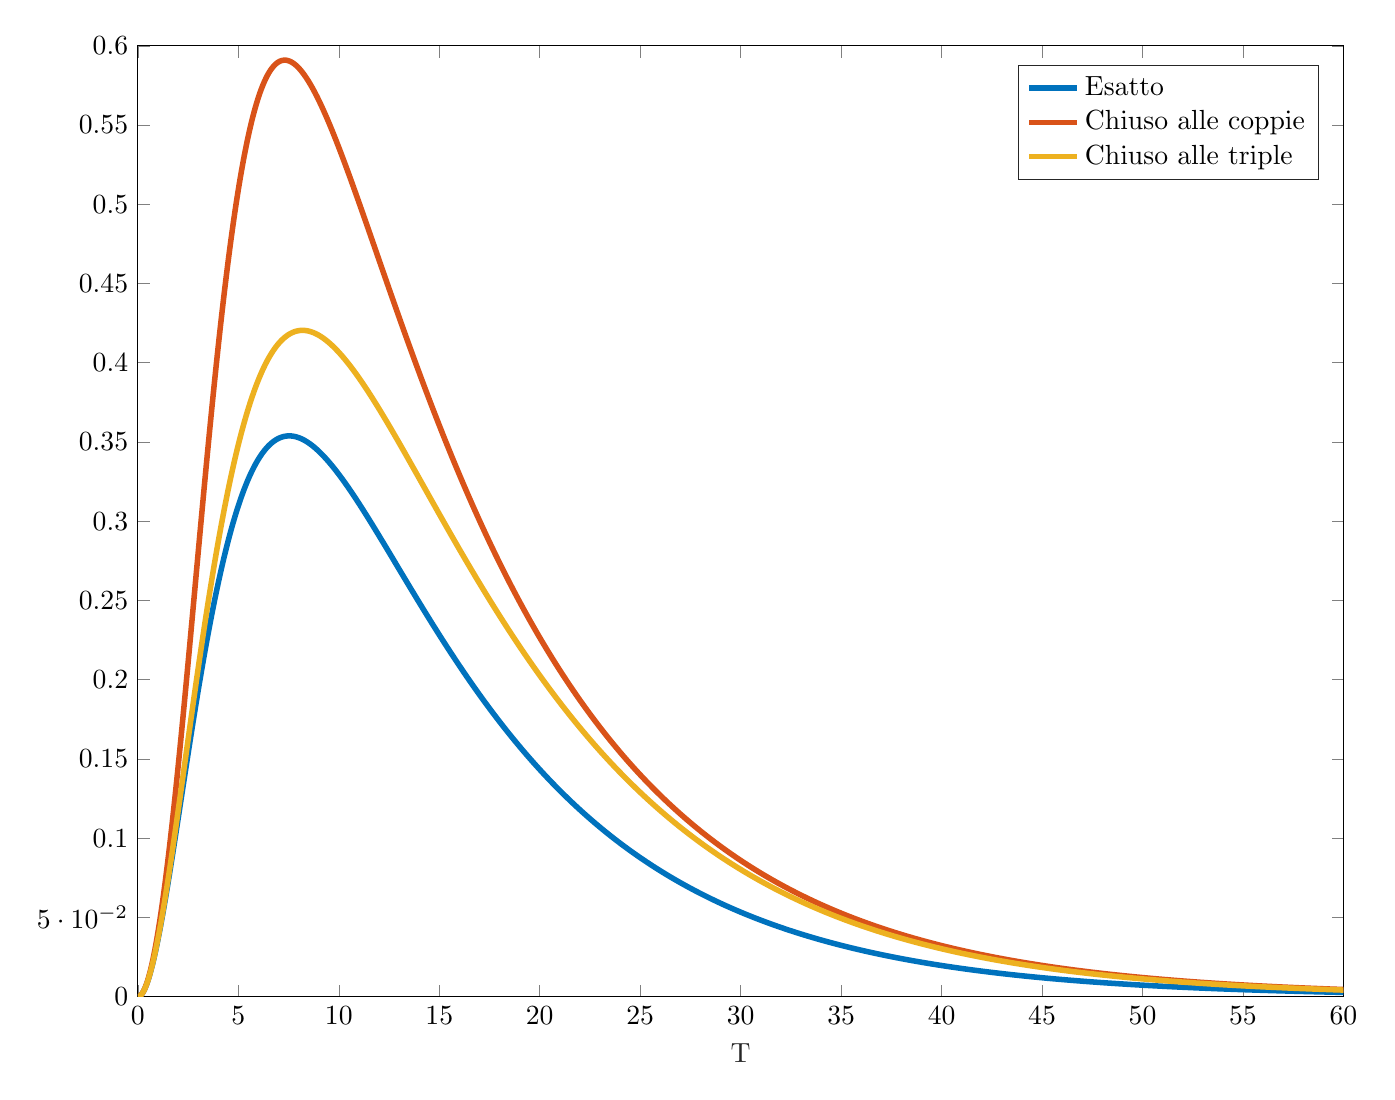
\begin{tikzpicture}

\begin{axis}[%
width=6.028in,
height=4.754in,
at={(1.011in,0.642in)},
scale only axis,
xmin=0,
xmax=60,
xlabel style={font=\color{white!15!black}},
xlabel={T},
ymin=0,
ymax=0.6,
axis background/.style={fill=white},
legend style={legend cell align=left, align=left, draw=white!15!black}
]
\addplot [color=mycolor1, line width=2.0pt]
  table[row sep=crcr]{%
0	0\\
0.00199053585276749	1.7822949683299e-07\\
0.00398107170553497	7.12633991639908e-07\\
0.00597160755830246	1.60278739921317e-06\\
0.00796214341106994	2.84826351211917e-06\\
0.0123567669950473	6.85404761850254e-06\\
0.0167513905790247	1.25850776445797e-05\\
0.0211460141630021	2.00367609805587e-05\\
0.0255406377469794	2.92045024183025e-05\\
0.0299388563931551	4.00933033485715e-05\\
0.0343370750393307	5.26917541687384e-05\\
0.0387352936855064	6.69952408030554e-05\\
0.043133512331682	8.29991469237719e-05\\
0.0475471725191068	0.000100763977079564\\
0.0519608327065316	0.000120231866818614\\
0.0563744928939564	0.000141398144414795\\
0.0607881530813811	0.000164258136209499\\
0.0652173199794049	0.000188896387840148\\
0.0696464868774286	0.000215230840277953\\
0.0740756537754524	0.000243256764792927\\
0.0785048206734761	0.000272969431043284\\
0.0829496187548012	0.000304477876436747\\
0.0873944168361263	0.000337675440822983\\
0.0918392149174515	0.000372557338934743\\
0.0962840129987766	0.000409118784214723\\
0.100744568101794	0.000447493511385649\\
0.105205123204811	0.00048755005287698\\
0.109665678307829	0.000529283567353318\\
0.114126233410846	0.000572689212512028\\
0.118602673075784	0.000617925628608725\\
0.123079112740721	0.000664836331901418\\
0.127555552405659	0.000713416425457245\\
0.132031992070596	0.000763661011700012\\
0.136524445545197	0.000815753845278292\\
0.141016899019798	0.000869513216851611\\
0.1455093524944	0.000924934174362011\\
0.150001805969001	0.000982011765433221\\
0.154510404254387	0.00104095506901093\\
0.159019002539772	0.00110155693968075\\
0.163527600825158	0.00116381237073368\\
0.168036199110544	0.00122771635546855\\
0.172561074936287	0.00129350350713688\\
0.17708595076203	0.00136094103361318\\
0.181610826587773	0.00143002387401335\\
0.186135702413515	0.00150074696778841\\
0.190676990405524	0.00157337067541191\\
0.195218278397533	0.0016476363445853\\
0.199759566389542	0.00172353886072682\\
0.204300854381551	0.00180107310991831\\
0.208858690959197	0.00188052541170688\\
0.213416527536843	0.0019616110411076\\
0.217974364114488	0.00204432483032052\\
0.222532200692134	0.0021286616125389\\
0.227106724202768	0.00221493388091906\\
0.231681247713401	0.00230283062264764\\
0.236255771224035	0.00239234661718764\\
0.240830294734669	0.0024834766453261\\
0.245421645441331	0.0025765595886291\\
0.250012996147992	0.00267125793099609\\
0.254604346854654	0.00276756639963606\\
0.259195697561315	0.00286547972341409\\
0.263804017673384	0.00296536338805228\\
0.268412337785452	0.0030668531577369\\
0.273020657897521	0.00316994370790795\\
0.27762897800959	0.0032746297159948\\
0.282254411746462	0.00338130348931587\\
0.286879845483334	0.00348957385422454\\
0.291505279220206	0.00359943543487873\\
0.296130712957079	0.00371088285776032\\
0.300773406613671	0.00382433547112046\\
0.305416100270264	0.00393937494346342\\
0.310058793926856	0.00405599584815389\\
0.314701487583449	0.00417419276121634\\
0.319361589521735	0.00429441229130397\\
0.324021691460022	0.00441620872887048\\
0.328681793398309	0.00453957659697822\\
0.333341895336596	0.00466451042168647\\
0.338019556071109	0.00479148429396836\\
0.342697216805623	0.00492002490358779\\
0.347374877540136	0.00505012672379765\\
0.35205253827465	0.00518178423118626\\
0.356747910447269	0.00531549922049169\\
0.361443282619888	0.00545077055855654\\
0.366138654792507	0.00558759266931946\\
0.370834026965126	0.00572595998039428\\
0.375547265516765	0.00586640221680881\\
0.380260504068404	0.00600839019523782\\
0.384973742620042	0.00615191829080272\\
0.389686981171681	0.00629698088264131\\
0.394418243246227	0.00644413584998692\\
0.399149505320772	0.00659282573459474\\
0.403880767395317	0.0067430448632684\\
0.408612029469863	0.00689478756717048\\
0.41336147459102	0.00704864010920734\\
0.418110919712177	0.00720401652597503\\
0.422860364833334	0.00736091109646086\\
0.427609809954491	0.0075193181043551\\
0.432377599961091	0.00767985242376575\\
0.437145389967691	0.00784189935773421\\
0.44191317997429	0.00800545313793538\\
0.44668096998089	0.00817050800109258\\
0.451467269141767	0.00833770766384279\\
0.456253568302644	0.00850640846349847\\
0.461039867463521	0.00867660458492832\\
0.465826166624398	0.00884829021839637\\
0.47063114173014	0.00902213815769364\\
0.475436116835881	0.00919747553893355\\
0.480241091941623	0.00937429650068697\\
0.485046067047365	0.00955259518726855\\
0.489869887370685	0.00973307370281882\\
0.494693707694006	0.00991502974813026\\
0.499517528017326	0.0100984574159869\\
0.504341348340647	0.0102833508052665\\
0.509184185682064	0.0104704415650874\\
0.51402702302348	0.0106589977253382\\
0.518869860364897	0.0108490133335296\\
0.523712697706314	0.0110404824436177\\
0.528574726619363	0.0112341664929077\\
0.533436755532412	0.011429303596298\\
0.53829878444546	0.0116258877565419\\
0.543160813358509	0.0118239129831912\\
0.548042211039569	0.0120241707405318\\
0.55292360872063	0.0122258689886733\\
0.55780500640169	0.01242900168613\\
0.56268640408275	0.0126335627985692\\
0.56758735048985	0.0128403740605406\\
0.572488296896949	0.0130486130330867\\
0.577389243304049	0.013258273631004\\
0.582290189711149	0.0134693497765985\\
0.587210867601438	0.0136826937191977\\
0.592131545491728	0.0138974523752264\\
0.597052223382018	0.0141136196162876\\
0.601972901272307	0.0143311893218511\\
0.606913496388328	0.0145510445083023\\
0.611854091504349	0.0147723011941749\\
0.61679468662037	0.0149949532084038\\
0.621735281736391	0.0152189943881514\\
0.626695982628195	0.0154453387607953\\
0.631656683519999	0.0156730712018817\\
0.636617384411802	0.0159021854982077\\
0.641578085303606	0.0161326754451591\\
0.646559083672327	0.0163654863400477\\
0.651540082041047	0.0165996716554555\\
0.656521080409768	0.0168352251365739\\
0.661502078778488	0.0170721405375458\\
0.666503569383853	0.0173113946798649\\
0.671505059989219	0.0175520093777441\\
0.676506550594584	0.0177939783353041\\
0.68150804119995	0.0180372952659821\\
0.686530221876942	0.0182829687696425\\
0.691552402553934	0.0185299887467229\\
0.696574583230927	0.0187783488608115\\
0.701596763907919	0.0190280427851802\\
0.706639835866396	0.0192801111661346\\
0.711682907824873	0.0195335117211375\\
0.71672597978335	0.0197882380737862\\
0.721769051741827	0.0200442838577301\\
0.72683321952555	0.0203027220311834\\
0.731897387309272	0.0205624778619397\\
0.736961555092995	0.0208235449341491\\
0.742025722876718	0.0210859168423846\\
0.747111194287107	0.021350699117281\\
0.752196665697496	0.0216167843151089\\
0.757282137107885	0.0218841659811192\\
0.762367608518274	0.0221528376713582\\
0.767474594900923	0.0224239377630902\\
0.772581581283573	0.0226963258255833\\
0.777688567666222	0.0229699953657403\\
0.782795554048871	0.0232449399016338\\
0.78792427039055	0.0235223309356013\\
0.793052986732229	0.0238009947701614\\
0.798181703073909	0.0240809248744226\\
0.803310419415588	0.0243621147290403\\
0.808461084325784	0.0246457692377514\\
0.81361174923598	0.0249306811586031\\
0.818762414146177	0.0252168439234676\\
0.823913079056373	0.0255042509761424\\
0.82908591482452	0.0257941408997806\\
0.834258750592667	0.0260852726284916\\
0.839431586360813	0.0263776395574727\\
0.84460442212896	0.0266712350942269\\
0.849799655005291	0.0269673317936489\\
0.854994887881621	0.0272646544721845\\
0.860190120757951	0.0275631964889205\\
0.865385353634282	0.0278629512156326\\
0.870603213699137	0.0281652254623746\\
0.875821073763992	0.0284687096429592\\
0.881038933828848	0.0287733970809315\\
0.886256793893703	0.0290792811129109\\
0.891497515445601	0.0293877031083246\\
0.896738236997499	0.0296973187726762\\
0.901978958549397	0.0300081213945414\\
0.907219680101295	0.0303201042759573\\
0.912483501408722	0.0306346436336498\\
0.917747322716149	0.0309503601752191\\
0.923011144023576	0.0312672471548477\\
0.928274965331004	0.0315852978405694\\
0.933562128954513	0.0319059236013823\\
0.938849292578023	0.0322277098403928\\
0.944136456201532	0.0325506497779706\\
0.949423619825042	0.0328747366487286\\
0.954734372782572	0.0332014172870096\\
0.960045125740102	0.0335292414767102\\
0.965355878697632	0.0338582024049715\\
0.970666631655162	0.0341882932735724\\
0.976001225418392	0.0345209966929383\\
0.981335819181621	0.034854826515271\\
0.98667041294485	0.0351897758950715\\
0.99200500670808	0.0355258380018755\\
0.997363697280812	0.0358645315353193\\
1.00272238785355	0.0362043341009664\\
1.00808107842628	0.0365452388212707\\
1.01343976899901	0.0368872388341203\\
1.0188228172289	0.037231889258643\\
1.02420586545878	0.0375776311216919\\
1.02958891368867	0.037924457514271\\
1.03497196191855	0.0382723615432202\\
1.04037963341625	0.0386229350696379\\
1.04578730491395	0.0389745822172536\\
1.05119497641164	0.0393272960462231\\
1.05660264790934	0.0396810696329432\\
1.06203521338424	0.0400375319217814\\
1.06746777885913	0.0403950497901334\\
1.07290034433402	0.0407536162679132\\
1.07833290980891	0.041113224401683\\
1.08379064506731	0.041475540557303\\
1.08924838032571	0.0418388940255831\\
1.09470611558411	0.0422032778068064\\
1.10016385084252	0.0425686849183151\\
1.1056470369148	0.0429368194907472\\
1.11113022298707	0.0433059728829442\\
1.11661340905935	0.0436761380661753\\
1.12209659513163	0.044047308029181\\
1.12760551858231	0.0444212250280102\\
1.13311444203298	0.0447961421268009\\
1.13862336548365	0.0451720522684289\\
1.14413228893432	0.0455489484136572\\
1.14966724184116	0.0459286112995448\\
1.15520219474799	0.0463092553376902\\
1.16073714765482	0.0466908734432023\\
1.16627210056166	0.0470734585494963\\
1.17183338076584	0.0474588302433864\\
1.17739466097002	0.0478451639129115\\
1.18295594117419	0.0482324524460456\\
1.18851722137837	0.0486206887494906\\
1.19410513262804	0.0490117316343535\\
1.19969304387772	0.049403717088219\\
1.20528095512739	0.0497966379725634\\
1.21086886637706	0.0501904871680156\\
1.21648371859449	0.0505871630988377\\
1.22209857081192	0.0509847619608945\\
1.22771342302936	0.0513832765898067\\
1.23332827524679	0.0517826998407763\\
1.23897038457538	0.0521849701387789\\
1.24461249390397	0.0525881434978711\\
1.25025460323256	0.0529922127284671\\
1.25589671256115	0.0533971706609938\\
1.26156640151281	0.0538049961141078\\
1.26723609046446	0.0542137045244657\\
1.27290577941612	0.0546232886779301\\
1.27857546836778	0.0550337413808108\\
1.28427306633634	0.0554470822701269\\
1.28997066430491	0.0558612857778406\\
1.29566826227347	0.056276344665923\\
1.30136586024204	0.0566922517172312\\
1.30709170327692	0.0571110677899438\\
1.31281754631181	0.0575307259056938\\
1.31854338934669	0.0579512188032283\\
1.32426923238158	0.0583725392426218\\
1.33002366371043	0.0587967897381747\\
1.33577809503928	0.0592218614633908\\
1.34153252636813	0.0596477471344669\\
1.34728695769699	0.0600744394893725\\
1.35307032782915	0.0605040831349718\\
1.35885369796131	0.060934526957224\\
1.36463706809348	0.0613657636504559\\
1.37042043822564	0.0617977859312162\\
1.37622881553645	0.0622324596390813\\
1.38203719284726	0.0626679110854667\\
1.38784557015807	0.0631041329597008\\
1.39365394746888	0.06354111797372\\
1.39948194569202	0.0639803388396922\\
1.40530994391516	0.0644203133789047\\
1.41113794213829	0.0648610342977984\\
1.41696594036143	0.0653024943257203\\
1.4228137248248	0.0657461887088551\\
1.42866150928816	0.0661906126324523\\
1.43450929375153	0.066635758821069\\
1.44035707821489	0.0670816200224627\\
1.44622478964653	0.0675297119422864\\
1.45209250107816	0.0679785091980472\\
1.45796021250979	0.0684280045335172\\
1.46382792394143	0.0688781907159599\\
1.46971570462452	0.06933060380475\\
1.4756034853076	0.0697836979560401\\
1.48149126599069	0.0702374659339126\\
1.48737904667378	0.0706919005262287\\
1.49328704060906	0.0711485580486936\\
1.49919503454433	0.0716058722941636\\
1.50510302847961	0.0720638360481231\\
1.51101102241489	0.0725224421201197\\
1.51693937480906	0.0729832669409242\\
1.52286772720322	0.0734447240819047\\
1.52879607959739	0.0739068063510373\\
1.53472443199155	0.0743695065806426\\
1.540673290528	0.0748344212698549\\
1.54662214906446	0.0752999438160608\\
1.55257100760091	0.0757660670508118\\
1.55851986613736	0.0762327838302813\\
1.56448937947106	0.0767017105536235\\
1.57045889280476	0.077171220613061\\
1.57642840613847	0.077641306864804\\
1.58239791947216	0.0781119621899579\\
1.58838823791446	0.0785848227682172\\
1.59437855635675	0.0790582421067338\\
1.60036887479904	0.0795322130874562\\
1.60635919324133	0.0800067286174983\\
1.61237046959671	0.0804834445995198\\
1.61838174595208	0.0809606947139292\\
1.62439302230746	0.0814384718694869\\
1.63040429866284	0.0819167690003855\\
1.63643668672632	0.082397261551219\\
1.6424690747898	0.0828782635571478\\
1.64850146285328	0.0833597679548181\\
1.65453385091676	0.0838417677065706\\
1.66058750665404	0.0843259577069938\\
1.66664116239132	0.0848106324386069\\
1.67269481812859	0.0852957848670103\\
1.67874847386587	0.0857814079837585\\
1.68482355500326	0.086269216004294\\
1.69089863614064	0.0867574839882173\\
1.69697371727803	0.087246204931149\\
1.70304879841541	0.0877353718549195\\
1.70914546464501	0.0882267181784857\\
1.71524213087462	0.088718499656472\\
1.72133879710422	0.0892107093155815\\
1.72743546333383	0.0897033402089795\\
1.73355387572031	0.090198144789141\\
1.73967228810678	0.0906933596762203\\
1.74579070049326	0.0911889779290641\\
1.75190911287974	0.0916849926332298\\
1.75804943463327	0.0921831751622365\\
1.76418975638681	0.0926817431148547\\
1.77033007814035	0.0931806895831316\\
1.77647039989388	0.0936800076860703\\
1.78263279664118	0.0941814876231251\\
1.78879519338848	0.0946833280674174\\
1.79495759013578	0.0951855221452476\\
1.80111998688309	0.0956880630101131\\
1.80730462566597	0.0961927595059203\\
1.81348926444885	0.0966977915621178\\
1.81967390323173	0.0972031523403108\\
1.82585854201462	0.0977088350295388\\
1.83206559217232	0.0982166670034985\\
1.83827264233002	0.0987248095632161\\
1.84447969248772	0.0992332559066485\\
1.85068674264543	0.0997419992594213\\
1.85691637550678	0.100252885380191\\
1.86314600836813	0.100764057086932\\
1.86937564122948	0.101275507615001\\
1.87560527409083	0.101787230227648\\
1.88185766319929	0.102301088936961\\
1.88811005230775	0.102815208209947\\
1.89436244141622	0.103329581320398\\
1.90061483052468	0.103844201570231\\
1.90689015093446	0.104360951030282\\
1.91316547134424	0.104877936011757\\
1.91944079175402	0.105395149827927\\
1.92571611216381	0.105912585820409\\
1.93201454150218	0.106432144006178\\
1.93831297084055	0.106951912653814\\
1.94461140017892	0.107471885117105\\
1.9509098295173	0.107992054778401\\
1.95723154808653	0.108514339491407\\
1.96355326665576	0.109036809592037\\
1.96987498522499	0.109559458475624\\
1.97619670379422	0.110082279566281\\
1.98254189319299	0.110607208325653\\
1.98888708259176	0.111132297386234\\
1.99523227199053	0.111657540185934\\
2.0015774613893	0.112182930191658\\
2.00794630624256	0.112710420381656\\
2.01431515109582	0.113238045776883\\
2.02068399594908	0.113765799858857\\
2.02705284080234	0.114293676138296\\
2.03344552746868	0.114823644906098\\
2.03983821413503	0.11535372377611\\
2.04623090080137	0.115883906274483\\
2.05262358746771	0.116414185956769\\
2.05904030495676	0.116946550292829\\
2.06545702244581	0.117478999623595\\
2.07187373993486	0.118011527520871\\
2.07829045742391	0.118544127586065\\
2.084731396657	0.119078804267171\\
2.0911723358901	0.119613540833507\\
2.0976132751232	0.120148330903553\\
2.1040542143563	0.12068316812559\\
2.11051956957009	0.12122007383553\\
2.11698492478388	0.121757014321785\\
2.12345027999767	0.12229398325053\\
2.12991563521146	0.122830974317928\\
2.13640560238783	0.123370025521238\\
2.1428955695642	0.123909086394997\\
2.14938553674057	0.124448150654087\\
2.15587550391694	0.124987212043569\\
2.16239028199053	0.125528325089654\\
2.16890506006412	0.12606942270586\\
2.17541983813771	0.126610498656792\\
2.1819346162113	0.127151546737412\\
2.18847440630977	0.1276946378012\\
2.19501419640825	0.128237688342795\\
2.20155398650673	0.128780692177532\\
2.20809377660521	0.129323643151286\\
2.21465878275268	0.129868628295239\\
2.22122378890015	0.130413547835157\\
2.22778879504762	0.130958395638113\\
2.23435380119508	0.131503165601899\\
2.24094422983074	0.132049960739475\\
2.24753465846639	0.132596665204097\\
2.25412508710205	0.133143272915586\\
2.2607155157377	0.13368977782465\\
2.2673315759421	0.134238298742397\\
2.27394763614649	0.134786703933639\\
2.28056369635089	0.135334987371944\\
2.28717975655528	0.13588314306194\\
2.29382166035897	0.136433305448228\\
2.30046356416266	0.136983327072242\\
2.30710546796636	0.137533201962302\\
2.31374737177005	0.138082924177949\\
2.32041533418655	0.13863464362859\\
2.32708329660306	0.13918619730137\\
2.33375125901957	0.139737579280361\\
2.34041922143607	0.140288783681014\\
2.34711345989709	0.140841975655293\\
2.3538076983581	0.141394976858727\\
2.36050193681912	0.141947781432133\\
2.36719617528013	0.142500383547867\\
2.37391691043736	0.143054963437569\\
2.3806376455946	0.143609327588407\\
2.38735838075183	0.144163470198944\\
2.39407911590907	0.144717385499429\\
2.40082657131283	0.145273268604641\\
2.40757402671659	0.145828911030314\\
2.41432148212035	0.146384307033746\\
2.42106893752412	0.146939450904073\\
2.42784333963791	0.147496552436712\\
2.4346177417517	0.148053388378842\\
2.4413921438655	0.148609953047493\\
2.44816654597929	0.149166240791669\\
2.4549681243632	0.149724475892727\\
2.4617697027471	0.150282420524358\\
2.46857128113101	0.15084006906431\\
2.47537285951492	0.151397415922448\\
2.48220184698832	0.15195669967724\\
2.48903083446173	0.15251566811806\\
2.49585982193513	0.153074315684363\\
2.50268880940853	0.153632636847854\\
2.50954544177924	0.154192884265536\\
2.51640207414995	0.154752791561409\\
2.52325870652066	0.155312353237623\\
2.53011533889137	0.155871563828708\\
2.53699985562036	0.156432689898206\\
2.54388437234935	0.156993451077035\\
2.55076888907833	0.157553841931022\\
2.55765340580732	0.158113857058503\\
2.5645660494942	0.158675776707669\\
2.57147869318108	0.159237306738586\\
2.57839133686796	0.159798441781744\\
2.58530398055484	0.160359176500262\\
2.59224499685821	0.16092180459078\\
2.59918601316159	0.161484018379066\\
2.60612702946496	0.162045812561256\\
2.61306804576833	0.162607181866231\\
2.62003768421203	0.163170433260129\\
2.62700732265572	0.163733245713629\\
2.63397696109942	0.164295613989492\\
2.64094659954311	0.164857532883338\\
2.64794511298781	0.165421322400728\\
2.65494362643251	0.165984648387643\\
2.6619421398772	0.166547505674449\\
2.6689406533219	0.167109889124479\\
2.67596829852112	0.167674131588995\\
2.68299594372033	0.168237885983242\\
2.69002358891955	0.168801147206172\\
2.69705123411877	0.169363910189805\\
2.70410827073433	0.169928520349816\\
2.71116530734989	0.170492617952379\\
2.71822234396545	0.17105619796601\\
2.72527938058101	0.17161925539239\\
2.73236607296869	0.172184148064524\\
2.73945276535637	0.172748503746725\\
2.74653945774405	0.173312317478044\\
2.75362615013173	0.173875584330795\\
2.76074276611797	0.174440674301384\\
2.76785938210422	0.175005202906485\\
2.77497599809046	0.175569165256664\\
2.78209261407671	0.176132556495839\\
2.78923942490227	0.17669775851668\\
2.79638623572783	0.177262374855673\\
2.80353304655339	0.177826400695873\\
2.81067985737896	0.178389831253774\\
2.81785713902212	0.178955060146569\\
2.82503442066529	0.179519679102398\\
2.83221170230846	0.180083683377779\\
2.83938898395163	0.18064706826275\\
2.84659701614953	0.181212238840401\\
2.85380504834743	0.181776775289409\\
2.86101308054533	0.182340672940731\\
2.86822111274323	0.182903927158917\\
2.87546017926332	0.18346895424622\\
2.88269924578341	0.184033323078808\\
2.88993831230351	0.184597029063049\\
2.8971773788236	0.185160067638973\\
2.90444776780364	0.185724866098001\\
2.91171815678368	0.186288982243949\\
2.91898854576373	0.186852411559568\\
2.92625893474377	0.187415149561337\\
2.93356093845992	0.187979634271801\\
2.94086294217606	0.188543412680673\\
2.94816494589221	0.189106480348063\\
2.95546694960836	0.189668832867867\\
2.96280086487659	0.190232918756606\\
2.97013478014483	0.190796274427175\\
2.97746869541306	0.191358895518011\\
2.9848026106813	0.191920777701399\\
2.99216873909201	0.192484379758104\\
2.99953486750271	0.193047227754021\\
3.00690099591342	0.193609317406891\\
3.01426712432413	0.194170644468351\\
3.02166577186631	0.194733677714194\\
3.02906441940849	0.195295933132706\\
3.03646306695067	0.195857406521901\\
3.04386171449286	0.196418093713738\\
3.05129319192691	0.196980473227474\\
3.05872466936097	0.19754205122545\\
3.06615614679503	0.198102823586926\\
3.07358762422909	0.198662786225152\\
3.08105224696524	0.199224427131048\\
3.0885168697014	0.199785242912944\\
3.09598149243755	0.200345229532325\\
3.1034461151737	0.200904382984697\\
3.11094420406679	0.201465200509217\\
3.11844229295988	0.202025169383599\\
3.12594038185297	0.202584285652525\\
3.13343847074605	0.203142545394727\\
3.14097035080817	0.203702454766353\\
3.14850223087028	0.204261492046012\\
3.1560341109324	0.204819653362557\\
3.16356599099451	0.205376934878918\\
3.17113199342146	0.205935851476072\\
3.17869799584842	0.206493872625496\\
3.18626399827537	0.20705099454119\\
3.19383000070233	0.207607213471252\\
3.20143046110215	0.208165052685973\\
3.20903092150198	0.208721973185447\\
3.21663138190181	0.209277971269797\\
3.22423184230164	0.209833043273262\\
3.2318671021242	0.210389720613092\\
3.23950236194676	0.210945456060259\\
3.24713762176933	0.21150024600199\\
3.25477288159189	0.212054086859637\\
3.26244328804483	0.212609517935818\\
3.27011369449776	0.213163984033911\\
3.2777841009507	0.213717481629223\\
3.28545450740363	0.214270007231193\\
3.29316041266953	0.214824107696851\\
3.30086631793543	0.215377220193082\\
3.30857222320133	0.215929341284257\\
3.31627812846722	0.216480467568877\\
3.32401989110489	0.217033153215368\\
3.33176165374256	0.217584827996945\\
3.33950341638023	0.218135488568027\\
3.3472451790179	0.218685131617155\\
3.35502316313618	0.21923631830838\\
3.36280114725446	0.219786471337052\\
3.37057913137275	0.220335587448621\\
3.37835711549103	0.220883663422646\\
3.38617169154667	0.221433267146064\\
3.3939862676023	0.221981814508943\\
3.40180084365794	0.22252930234875\\
3.40961541971357	0.223075727537046\\
3.41746696420648	0.223623664375271\\
3.42531850869938	0.224170522256531\\
3.43317005319229	0.224716298111303\\
3.4410215976852	0.225260988904131\\
3.44891049346576	0.225807175049859\\
3.45679938924632	0.226352259745611\\
3.46468828502688	0.226896240015862\\
3.47257718080744	0.227439112919129\\
3.48050381756295	0.227983464701382\\
3.48843045431847	0.2285266926458\\
3.49635709107398	0.229068793871853\\
3.50428372782949	0.229609765533017\\
3.51224850159594	0.230152199375446\\
3.52021327536239	0.23069348709924\\
3.52817804912884	0.23123362591986\\
3.53614282289529	0.231772613086733\\
3.54414613607264	0.232313045501611\\
3.55214944924998	0.232852309626045\\
3.56015276242733	0.233390402772492\\
3.56815607560468	0.233927322287327\\
3.57619833889781	0.234465669998337\\
3.58424060219095	0.235002827357494\\
3.59228286548408	0.235538791775251\\
3.60032512877721	0.236073560695929\\
3.60840675922679	0.236609740495042\\
3.61648838967638	0.237144707993296\\
3.62457002012596	0.237678460700149\\
3.63265165057554	0.23821099615887\\
3.64077307248204	0.238744924960261\\
3.64889449438855	0.239277619625967\\
3.65701591629505	0.239809077765467\\
3.66513733820155	0.240339297021984\\
3.67329898353354	0.240870891879215\\
3.68146062886554	0.241401230881812\\
3.68962227419754	0.241930311740289\\
3.69778391952953	0.242458132198835\\
3.70598622860803	0.242987310338433\\
3.71418853768653	0.243515211021843\\
3.72239084676502	0.244041832061637\\
3.73059315584352	0.244567171303982\\
3.73883657626523	0.245093850044177\\
3.74707999668693	0.24561922984592\\
3.75532341710863	0.246143308624868\\
3.76356683753034	0.24666608433019\\
3.77185182516863	0.247190181135091\\
3.78013681280692	0.247712957640202\\
3.78842180044522	0.248234411865297\\
3.79670678808351	0.248754541863568\\
3.80503380745825	0.249275974354245\\
3.81336082683299	0.249796065306283\\
3.82168784620774	0.250314812844608\\
3.83001486558248	0.25083221512747\\
3.83838438958511	0.251350901051855\\
3.84675391358775	0.251868224322941\\
3.85512343759039	0.252384183171852\\
3.86349296159302	0.252898775862928\\
3.8719054722877	0.253414633132844\\
3.88031798298237	0.253929106760488\\
3.88873049367705	0.25444219508423\\
3.89714300437172	0.254953896475545\\
3.90559899284027	0.255466843142865\\
3.91405498130882	0.255978385306229\\
3.92251096977737	0.25648852141231\\
3.93096695824593	0.256997249940768\\
3.93946692479213	0.2575072041959\\
3.94796689133833	0.258015733214279\\
3.95646685788454	0.258522835551945\\
3.96496682443074	0.259028509797801\\
3.97351127881372	0.259535389969321\\
3.98205573319669	0.260040824301765\\
3.99060018757967	0.260544811461612\\
3.99914464196265	0.261047350148068\\
4.00773410425464	0.26155107473823\\
4.01632356654662	0.262053333018832\\
4.02491302883861	0.262554123767866\\
4.0335024911306	0.263053445795917\\
4.04213749081375	0.263553933411006\\
4.05077249049689	0.264052934379626\\
4.05940749018004	0.264550447592377\\
4.06804248986318	0.265046471972299\\
4.07672356764034	0.265543641412176\\
4.08540464541749	0.266039304003458\\
4.09408572319465	0.26653345875044\\
4.10276680097181	0.267026104689711\\
4.11149450824228	0.26751987489828\\
4.12022221551276	0.268012118192356\\
4.12894992278323	0.26850283369104\\
4.1376776300537	0.268992020545566\\
4.14645252883691	0.269482310588696\\
4.15522742762012	0.269971053789234\\
4.16400232640333	0.270458249382202\\
4.17277722518654	0.270943896634584\\
4.18159988926615	0.271430625745956\\
4.19042255334575	0.271915788225688\\
4.19924521742536	0.272399383425849\\
4.20806788150496	0.272881410730293\\
4.21693889629988	0.273364498283558\\
4.22580991109479	0.273845999556575\\
4.23468092588971	0.2743259140196\\
4.24355194068463	0.274804241174484\\
4.2524719033702	0.275283606669781\\
4.26139186605577	0.275761366378113\\
4.27031182874135	0.276237519889067\\
4.27923179142692	0.276712066823633\\
4.28820131218307	0.277187629933685\\
4.29717083293922	0.277661567893043\\
4.30614035369538	0.278133880411788\\
4.31510987445153	0.2786045672312\\
4.32412957614907	0.279076247760928\\
4.33314927784661	0.279546283920541\\
4.34216897954416	0.280014675541787\\
4.3511886812417	0.280481422487404\\
4.36025919971018	0.280949140365308\\
4.36932971817866	0.281415194799323\\
4.37840023664715	0.281879585744049\\
4.38747075511563	0.282342313184861\\
4.39659274002011	0.282805988484664\\
4.40571472492458	0.283267981413586\\
4.41483670982906	0.283728292050282\\
4.42395869473353	0.284186920503955\\
4.43313280988389	0.284646473434564\\
4.44230692503424	0.28510432521523\\
4.45148104018459	0.285560476049881\\
4.46065515533495	0.286014926172754\\
4.469882079136	0.286470277074369\\
4.47910900293706	0.286923908196023\\
4.48833592673811	0.287375819868147\\
4.49756285053916	0.287826012451236\\
4.50684327607396	0.288277081772282\\
4.51612370160877	0.288726412833611\\
4.52540412714357	0.289174006093409\\
4.53468455267837	0.289619862039669\\
4.54401918924822	0.290066570383598\\
4.55335382581807	0.290511522139111\\
4.56268846238792	0.290954717893413\\
4.57202309895777	0.291396158263252\\
4.58141267108196	0.291838426309707\\
4.59080224320616	0.292278919591421\\
4.60019181533036	0.292717638825905\\
4.60958138745456	0.293154584759936\\
4.61902663678989	0.293592333326223\\
4.62847188612523	0.294028289104579\\
4.63791713546056	0.294462452944122\\
4.6473623847959	0.294894825722955\\
4.65686406984621	0.295327975717076\\
4.66636575489653	0.295759315054243\\
4.67586743994685	0.296188844716511\\
4.68536912499717	0.296616565714622\\
4.69492802222378	0.297045038153114\\
4.7044869194504	0.297471682220597\\
4.71404581667701	0.297896499033403\\
4.72360471390363	0.298319489736252\\
4.73320764525141	0.298742591428161\\
4.74281057659919	0.29916385254918\\
4.75241350794698	0.299583274345783\\
4.76201643929476	0.300000858092349\\
4.77165794452804	0.300418271397608\\
4.78129944976131	0.300833834515817\\
4.79094095499459	0.301247548821007\\
4.80058246022786	0.30165941571457\\
4.81026314694842	0.302071099118429\\
4.81994383366897	0.302480922979367\\
4.82962452038952	0.302888888798503\\
4.83930520711008	0.303294998103758\\
4.84902565638322	0.303700909065285\\
4.85874610565637	0.304104951399363\\
4.86846655492951	0.304507126733728\\
4.87818700420266	0.304907436722363\\
4.88794780523678	0.305307533203412\\
4.89770860627089	0.305705752241743\\
4.90746940730501	0.306102095591256\\
4.91723020833913	0.306496565031541\\
4.92703195872998	0.306890805485238\\
4.93683370912084	0.307283159948193\\
4.9466354595117	0.307673630300041\\
4.95643720990256	0.308062218445548\\
4.96628051524823	0.30845056177983\\
4.97612382059389	0.308837010840906\\
4.98596712593956	0.309221567633732\\
4.99581043128522	0.309604234187836\\
5.00569590732134	0.309986639829006\\
5.01558138335745	0.31036714317773\\
5.02546685939356	0.310745746363893\\
5.03535233542967	0.311122451541387\\
5.04528060635073	0.311498879344567\\
5.05520887727179	0.31187339709777\\
5.06513714819285	0.312246007055439\\
5.07506541911391	0.312616711495453\\
5.08503711889176	0.312987121774831\\
5.0950088186696	0.313355614506573\\
5.10498051844744	0.313722192069321\\
5.11495221822528	0.314086856864582\\
5.12496799094167	0.314451210382843\\
5.13498376365806	0.314813639113888\\
5.14499953637444	0.315174145560223\\
5.15501530909083	0.315532732246646\\
5.16507580953502	0.315890990213315\\
5.17513630997921	0.316247316409436\\
5.18519681042339	0.316601713461061\\
5.19525731086758	0.316954184015958\\
5.2053632039849	0.317306308044146\\
5.21546909710223	0.317656493573266\\
5.22557499021955	0.318004743352618\\
5.23568088333688	0.318351060152634\\
5.24583284576096	0.318697012290215\\
5.25598480818505	0.319041019453184\\
5.26613677060914	0.319383084513811\\
5.27628873303322	0.319723210364912\\
5.28648745229033	0.320062953042444\\
5.29668617154743	0.320400744521465\\
5.30688489080453	0.320736587796951\\
5.31708361006163	0.321070485883841\\
5.32732978639303	0.321403981952254\\
5.33757596272443	0.321735520848064\\
5.34782213905582	0.322065105688716\\
5.35806831538722	0.322392739611023\\
5.36836266133408	0.322719952301214\\
5.37865700728095	0.323045202093047\\
5.38895135322782	0.323368492226213\\
5.39924569917468	0.323689825959177\\
5.40958894010065	0.324010718873724\\
5.41993218102661	0.324329643411026\\
5.43027542195257	0.324646602932822\\
5.44061866287853	0.324961600819022\\
5.45101153706255	0.325276137909782\\
5.46140441124658	0.325588701389991\\
5.4717972854306	0.325899294743252\\
5.48219015961463	0.326207921470737\\
5.49263341945276	0.326516067049904\\
5.50307667929089	0.326822234029264\\
5.51351993912902	0.327126426014125\\
5.52396319896715	0.327428646626752\\
5.53445761187213	0.32773036536511\\
5.54495202477712	0.328030100756806\\
5.5554464376821	0.328327856528714\\
5.56594085058709	0.328623636424052\\
5.57648719831941	0.328918893302735\\
5.58703354605173	0.32921216232914\\
5.59757989378405	0.32950344735159\\
5.60812624151637	0.329792752234129\\
5.61872532103302	0.330081512542028\\
5.62932440054967	0.330368280732022\\
5.63992348006633	0.330653060773784\\
5.65052255958298	0.330935856652084\\
5.66117518401188	0.331218085984166\\
5.67182780844078	0.331498319171329\\
5.68248043286967	0.33177656030452\\
5.69313305729857	0.332052813489157\\
5.70384005671797	0.332328477736891\\
5.71454705613736	0.332602142049887\\
5.72525405555675	0.332873810640318\\
5.73596105497615	0.333143487734188\\
5.74672327665992	0.333412553060722\\
5.75748549834369	0.333679614898646\\
5.76824772002746	0.333944677581329\\
5.77900994171123	0.334207745455329\\
5.78982825023888	0.33447017826791\\
5.80064655876654	0.334730604272931\\
5.81146486729419	0.33498902792495\\
5.82228317582184	0.335245453691067\\
5.83315845473553	0.335501220650853\\
5.84403373364921	0.335754977717684\\
5.8549090125629	0.336006729467326\\
5.86578429147658	0.336256480487432\\
5.87671744355088	0.336505548482196\\
5.88765059562518	0.336752603730981\\
5.89858374769948	0.336997650930805\\
5.90951689977378	0.337240694789915\\
5.92050884813521	0.337483030925991\\
5.93150079649664	0.337723351694139\\
5.94249274485807	0.337961661912699\\
5.9534846932195	0.338197966410573\\
5.96453638108293	0.338433537972386\\
5.97558806894636	0.338667091774498\\
5.98663975680979	0.338898632756669\\
5.99769144467322	0.339128165868544\\
6.00880383710542	0.339356940322759\\
6.01991622953761	0.33958369485445\\
6.0310286219698	0.339808434524918\\
6.042141014402	0.340031164404669\\
6.05331509935885	0.340253109384269\\
6.0644891843157	0.340473032506196\\
6.07566326927256	0.340690938953445\\
6.08683735422941	0.340906833917525\\
6.09807414230094	0.34112191717886\\
6.10931093037248	0.341334976874208\\
6.12054771844401	0.341546018308435\\
6.13178450651555	0.341755046794229\\
6.14308503319571	0.341963236223625\\
6.15438555987588	0.342169400604244\\
6.16568608655605	0.342373545363039\\
6.17698661323621	0.342575675934077\\
6.18835193888863	0.342776939506329\\
6.19971726454106	0.342976176771615\\
6.21108259019348	0.343173393279219\\
6.2224479158459	0.343368594584821\\
6.23387912710053	0.343562900348393\\
6.24531033835517	0.343755178770374\\
6.2567415496098	0.343945435522649\\
6.26817276086443	0.344133676282783\\
6.2796709718506	0.344320992338856\\
6.29116918283678	0.344506280241196\\
6.30266739382295	0.3446895457846\\
6.31416560480912	0.344870794768814\\
6.32573195844141	0.345051089248496\\
6.33729831207371	0.345229354983671\\
6.34886466570601	0.345405597892395\\
6.36043101933831	0.34557982389693\\
6.37206668825559	0.345753064930601\\
6.38370235717287	0.345924276849353\\
6.39533802609016	0.346093465694883\\
6.40697369500744	0.34626063751234\\
6.41867988207414	0.346426793191705\\
6.43038606914084	0.346590919605371\\
6.44209225620754	0.346753022919096\\
6.45379844327423	0.346913109301326\\
6.46557638449348	0.347072147674652\\
6.47735432571273	0.347229156849865\\
6.48913226693197	0.34738414311724\\
6.50091020815122	0.347537112768972\\
6.51276117329228	0.347689001798229\\
6.52461213843333	0.347838861914338\\
6.53646310357439	0.347986699532597\\
6.54831406871544	0.348132521069439\\
6.56023936237899	0.34827722859338\\
6.57216465604253	0.348419907705689\\
6.58408994970607	0.348560564947234\\
6.59601524336962	0.348699206859221\\
6.608016207688	0.348836700574063\\
6.62001717200638	0.348972166594139\\
6.63201813632476	0.349105611586476\\
6.64401910064313	0.349237042217634\\
6.65609711612489	0.349367289630464\\
6.66817513160664	0.349495510279822\\
6.68025314708839	0.349621710959544\\
6.69233116257014	0.34974589846217\\
6.70448764976455	0.349868866852896\\
6.71664413695897	0.349989809625007\\
6.72880062415338	0.35010873369983\\
6.7409571113478	0.35022564599657\\
6.75319353351478	0.350341302386531\\
6.76542995568177	0.350454934515151\\
6.77766637784875	0.350566549432\\
6.78990280001574	0.350676154183678\\
6.80222066442117	0.350784465285752\\
6.8145385288266	0.350890753695281\\
6.82685639323203	0.350995026590879\\
6.83917425763746	0.351097291147327\\
6.85157511856051	0.351198223329069\\
6.86397597948357	0.351297134597388\\
6.87637684040662	0.351394032260806\\
6.88877770132968	0.351488923623136\\
6.90126316148383	0.351582442850922\\
6.91374862163799	0.351673943153817\\
6.92623408179214	0.351763431971179\\
6.93871954194629	0.351850916736759\\
6.95129125486549	0.351936988525761\\
6.96386296778468	0.352021043586897\\
6.97643468070388	0.352103089491349\\
6.98900639362307	0.352183133803785\\
7.00166606764739	0.352261723173576\\
7.0143257416717	0.352338298219637\\
7.02698541569601	0.352412866646038\\
7.03964508972033	0.35248543614941\\
7.05239448925109	0.352556507554677\\
7.06514388878186	0.352625567246547\\
7.07789328831262	0.35269262306312\\
7.09064268784339	0.352757682834109\\
7.10348363709426	0.352821200108428\\
7.11632458634514	0.352882708484697\\
7.12916553559601	0.352942215936261\\
7.14200648484689	0.352999730427116\\
7.15494087138423	0.353055656717681\\
7.16787525792157	0.353109577129229\\
7.18080964445891	0.353161499771656\\
7.19374403099625	0.353211432744524\\
7.20677380774895	0.353259730434468\\
7.21980358450165	0.353306025467192\\
7.23283336125435	0.353350326090535\\
7.24586313800706	0.353392640540994\\
7.25899032889946	0.353433271181923\\
7.27211751979186	0.353471902588617\\
7.28524471068426	0.353508543148348\\
7.29837190157667	0.353543201236019\\
7.31159860422458	0.353576125459926\\
7.32482530687249	0.353607054072537\\
7.3380520095204	0.353635995602149\\
7.35127871216831	0.35366295856364\\
7.36460710304072	0.353688135997108\\
7.37793549391314	0.353711321640607\\
7.39126388478556	0.35373252416516\\
7.40459227565797	0.353751752227301\\
7.41802461355885	0.353769141393143\\
7.43145695145972	0.35378454278743\\
7.4448892893606	0.353797965225733\\
7.45832162726148	0.353809417508032\\
7.47186025959003	0.35381897572486\\
7.48539889191859	0.353826550383868\\
7.49893752424715	0.353832150447124\\
7.51247615657571	0.353835784859974\\
7.52612352432791	0.353837468128741\\
7.53977089208011	0.35383717224701\\
7.55341825983232	0.353834906325425\\
7.56706562758452	0.353830679456752\\
7.58082427117841	0.353824442339191\\
7.5945829147723	0.353816230670197\\
7.60834155836619	0.353806053711221\\
7.62210020196009	0.353793920704649\\
7.63597276754062	0.353779716191476\\
7.64984533312116	0.353763541915731\\
7.66371789870169	0.35374540729206\\
7.67759046428223	0.353725321714818\\
7.69157971106386	0.353703101081804\\
7.70556895784549	0.353678915662666\\
7.71955820462712	0.353652775027794\\
7.73354745140875	0.353624688726041\\
7.7476562591015	0.35359440137702\\
7.76176506679424	0.353562154403563\\
7.77587387448699	0.353527957534551\\
7.78998268217974	0.353491820476033\\
7.80421406003167	0.353453413769418\\
7.81844543788359	0.353413052782555\\
7.83267681573552	0.353370747405752\\
7.84690819358745	0.353326507505157\\
7.86126528820976	0.353279926568395\\
7.87562238283208	0.353231396875446\\
7.8899794774544	0.353180928481199\\
7.90433657207672	0.353128531415017\\
7.91882267896367	0.353073718934074\\
7.93330878585062	0.353016963397563\\
7.94779489273757	0.352958275028351\\
7.96228099962452	0.352897664022361\\
7.97689957365268	0.352834560014442\\
7.99151814768085	0.352769518824661\\
8.00613672170902	0.352702550847506\\
8.02075529573718	0.352633666449067\\
8.03550996276884	0.352562208013739\\
8.0502646298005	0.352488818439648\\
8.06501929683216	0.352413508296835\\
8.07977396386382	0.352336288125432\\
8.09466853533245	0.352256409161658\\
8.10956310680107	0.352174605267211\\
8.12445767826969	0.352090887191922\\
8.13935224973832	0.352005265654149\\
8.15439073744049	0.35191689655096\\
8.16942922514267	0.351826608885338\\
8.18446771284484	0.351734413591478\\
8.19950620054702	0.351640321570483\\
8.2146928332504	0.351543388862558\\
8.22987946595378	0.351444544115197\\
8.24506609865717	0.351343798451908\\
8.26025273136055	0.351241162961424\\
8.27559197362809	0.351135588942912\\
8.29093121589562	0.351028109556618\\
8.30627045816316	0.350918736120719\\
8.32160970043069	0.35080747991687\\
8.33710627308224	0.350693182212918\\
8.35260284573378	0.350576985954716\\
8.36809941838533	0.350458902660925\\
8.38359599103687	0.35033894381186\\
8.39925489573158	0.350215834885747\\
8.41491380042629	0.350090834352842\\
8.430572705121	0.349963953938605\\
8.44623160981571	0.349835205328252\\
8.46205815432056	0.349703191942671\\
8.4778846988254	0.34956929402296\\
8.49371124333024	0.349433523508257\\
8.50953778783509	0.349295892295475\\
8.52553761739547	0.34915487488178\\
8.54153744695585	0.349011980121519\\
8.55753727651623	0.348867220175019\\
8.57353710607661	0.348720607158308\\
8.58971623619016	0.348570479122112\\
8.60589536630372	0.348418481030364\\
8.62207449641727	0.34826462527279\\
8.63825362653082	0.348108924192648\\
8.65461848330403	0.347949571096118\\
8.67098334007723	0.347788355324967\\
8.68734819685043	0.34762528950733\\
8.70371305362364	0.347460386222592\\
8.72018188980809	0.347292592831934\\
8.73665072599255	0.347122963961679\\
8.75311956217701	0.346951512283014\\
8.76958839836146	0.346778250417062\\
8.78614348346302	0.346602269421402\\
8.80269856856458	0.346424484650271\\
8.81925365366614	0.346244908771212\\
8.83580873876771	0.346063554400636\\
8.85245111606455	0.345879463883055\\
8.86909349336139	0.345693601480292\\
8.88573587065824	0.345505979853203\\
8.90237824795508	0.345316611610455\\
8.91910883699713	0.345124491786593\\
8.93583942603918	0.344930632176372\\
8.95257001508123	0.34473504543063\\
8.96930060412328	0.344537744146977\\
8.98612034063892	0.344337675962106\\
9.00294007715455	0.344135900289318\\
9.01975981367019	0.343932429766136\\
9.03657955018582	0.343727276975844\\
9.05348938408815	0.343519342098702\\
9.07039921799048	0.343309732223399\\
9.08730905189281	0.343098459970885\\
9.10421888579513	0.342885537906871\\
9.12121978296026	0.342669818681566\\
9.13822068012539	0.342452457130689\\
9.15522157729052	0.342233465855393\\
9.17222247445565	0.342012857400611\\
9.18931541587169	0.34178943683006\\
9.20640835728774	0.341564406781241\\
9.22350129870378	0.341337779832316\\
9.24059424011982	0.34110956850427\\
9.25778022278737	0.340878530213245\\
9.27496620545493	0.340645915457859\\
9.29215218812249	0.340411736790126\\
9.30933817079004	0.340176006703945\\
9.32661820779546	0.33993743491279\\
9.34389824480088	0.33969731982985\\
9.3611782818063	0.339455673977868\\
9.37845831881172	0.339212509820552\\
9.39583344002363	0.338966489311163\\
9.41320856123555	0.338718958833359\\
9.43058368244747	0.338469930877525\\
9.44795880365938	0.338219417874108\\
9.46543005570071	0.337966033966248\\
9.48290130774205	0.337711173556463\\
9.50037255978338	0.337454849099721\\
9.51784381182471	0.337197072990174\\
9.53541225878365	0.336936411508148\\
9.55298070574258	0.336674307126193\\
9.57054915270152	0.336410772260838\\
9.58811759966045	0.336145819266939\\
9.60578432346384	0.335877966511259\\
9.62345104726722	0.335608704585671\\
9.64111777107061	0.335338045865281\\
9.658784494874	0.335066002662677\\
9.67655059520445	0.334791045389405\\
9.6943166955349	0.334514712796998\\
9.71208279586536	0.334237017216182\\
9.72984889619581	0.333957970914343\\
9.74771549159443	0.33367599629714\\
9.76558208699305	0.333392680325064\\
9.78344868239167	0.333108035281541\\
9.80131527779029	0.332822073385855\\
9.81928350543996	0.332533168998582\\
9.83725173308963	0.332242957327157\\
9.8552199607393	0.331951450604816\\
9.87318818838897	0.33165866099987\\
9.89125920482513	0.331362914785707\\
9.90933022126129	0.33106589545762\\
9.92740123769745	0.330767615195801\\
9.94547225413361	0.330468086114752\\
9.96364723590061	0.330165586356312\\
9.9818222176676	0.329861847746837\\
9.99999719943459	0.329556882410648\\
10.0181721812016	0.329250702405639\\
10.0364523247657	0.328941537707949\\
10.0547324683298	0.328631168508127\\
10.0730126118939	0.328319606871834\\
10.0912927554579	0.328006864797582\\
10.1096792783833	0.327691124050822\\
10.1280658013086	0.327374213230236\\
10.146452324234	0.327056144340071\\
10.1648388471593	0.326736929316713\\
10.1833329877765	0.326414701684792\\
10.2018271283938	0.326091338480386\\
10.220321269011	0.325766851643594\\
10.2388154096282	0.325441253045974\\
10.257418428294	0.325112627928829\\
10.2760214469598	0.32478290180723\\
10.2946244656257	0.324452086554435\\
10.3132274842915	0.324120193974498\\
10.3319406634311	0.323785260991743\\
10.3506538425707	0.323449261633106\\
10.3693670217104	0.323112207702343\\
10.38808020085	0.322774110933356\\
10.4069048454226	0.322432959901597\\
10.4257294899953	0.322090777177057\\
10.4445541345679	0.321747574491356\\
10.4633787791406	0.321403363505629\\
10.4823162175897	0.321056084407615\\
10.5012536560388	0.320707808348525\\
10.5201910944879	0.320358546985234\\
10.539128532937	0.32000831190353\\
10.5581801172831	0.319654994873401\\
10.5772317016292	0.319300715656755\\
10.5962832859753	0.318945485833154\\
10.6153348703214	0.318589316910481\\
10.6345019773376	0.318230052199976\\
10.6536690843538	0.317869860114696\\
10.67283619137	0.317508752154346\\
10.6920032983861	0.317146739746381\\
10.7112873293394	0.316781617718252\\
10.7305713602926	0.31641560315882\\
10.7498553912458	0.316048707485413\\
10.769139422199	0.315680942042566\\
10.7885418041401	0.315310053136061\\
10.8079441860811	0.314938306568057\\
10.8273465680222	0.314565713671027\\
10.8467489499633	0.314192285704117\\
10.8662711360792	0.313815720418554\\
10.8857933221952	0.313438332362405\\
10.9053155083112	0.313060132780826\\
10.9248376944271	0.312681132845138\\
10.9444811647161	0.312298981718272\\
10.9641246350051	0.311916042727739\\
10.9837681052941	0.311532327028952\\
11.0034115755831	0.311147845702993\\
11.02317783773	0.310760199286193\\
11.0429440998769	0.310371799923671\\
11.0627103620238	0.309982658678693\\
11.0824766241707	0.309592786539725\\
11.102367213876	0.309199735384577\\
11.1222578035813	0.308805966207861\\
11.1421483932866	0.308411489978322\\
11.1620389829919	0.308016317589452\\
11.182055464688	0.3076179522278\\
11.202071946384	0.307218903770255\\
11.22208842808	0.306819183088694\\
11.2421049097761	0.306418800979306\\
11.2622488777205	0.30601521189653\\
11.282392845665	0.305610974640484\\
11.3025368136094	0.305206099983853\\
11.3226807815539	0.304800598623219\\
11.3429428732039	0.304392097920854\\
11.363204964854	0.303982984619114\\
11.3834670565041	0.303573269371919\\
11.4037291481542	0.303162962756851\\
11.4240073959591	0.302751747421538\\
11.444285643764	0.302339960742818\\
11.464563891569	0.301927613095044\\
11.4848421393739	0.301514714777566\\
11.5051410232308	0.301100855009188\\
11.5254399070878	0.300686463875284\\
11.5457387909448	0.300271551481933\\
11.5660376748017	0.299856127861473\\
11.5863613245615	0.299439695216151\\
11.6066849743212	0.299022769999474\\
11.627008624081	0.298605362059437\\
11.6473322738407	0.298187481171496\\
11.6676846007299	0.297768546422854\\
11.6880369276191	0.297349156792186\\
11.7083892545083	0.29692932187876\\
11.7287415813975	0.296509051210455\\
11.7491263024508	0.296087684298775\\
11.7695110235041	0.29566589916054\\
11.7898957445574	0.295243705154907\\
11.8102804656107	0.294821111570748\\
11.8307011258767	0.294397381546999\\
11.8511217861426	0.293973268982398\\
11.8715424464086	0.293548783003947\\
11.8919631066745	0.293123932669421\\
11.9124230970895	0.292697907685015\\
11.9328830875046	0.292271534933825\\
11.9533430779196	0.291844823318058\\
11.9738030683347	0.291417781671719\\
11.9943056417768	0.290989528968619\\
12.014808215219	0.290560962414048\\
12.0353107886612	0.290132090692246\\
12.0558133621033	0.289702922420238\\
12.0763616495731	0.289272508285524\\
12.0969099370428	0.288841813404089\\
12.1174582245125	0.288410846248554\\
12.1380065119823	0.287979615225276\\
12.1586035338403	0.287547105020278\\
12.1792005556983	0.287114346406892\\
12.1997975775563	0.286681347652032\\
12.2203945994143	0.286248116957265\\
12.2410432774846	0.285813575103965\\
12.2616919555548	0.285378816454681\\
12.2823406336251	0.284943849076133\\
12.3029893116954	0.284508680970584\\
12.3236924799435	0.284072170945912\\
12.3443956481917	0.283635475048971\\
12.3650988164398	0.283198601151438\\
12.385801984688	0.282761557061398\\
12.406562398648	0.28232314139858\\
12.4273228126081	0.281884570132866\\
12.4480832265682	0.281445850945713\\
12.4688436405282	0.281006991455828\\
12.4896639845707	0.280566731774383\\
12.5104843286133	0.280126346136845\\
12.5313046726558	0.279685842038975\\
12.5521250166983	0.279245226914598\\
12.5730079121072	0.278803183918352\\
12.5938908075161	0.278361044019681\\
12.614773702925	0.277918814532893\\
12.6356565983338	0.277476502711155\\
12.6566046110283	0.277032736180354\\
12.6775526237227	0.27658890123499\\
12.6985006364172	0.27614500501191\\
12.7194486491116	0.275701054587593\\
12.7404642942679	0.275255623424837\\
12.7614799394242	0.27481015179503\\
12.7824955845805	0.274364646661309\\
12.8035112297368	0.273919114927201\\
12.8245969793381	0.273472077130889\\
12.8456827289394	0.273025026298414\\
12.8667684785407	0.272577969222742\\
12.887854228142	0.272130912637966\\
12.9090125143938	0.271682325353936\\
12.9301708006455	0.271233751970191\\
12.9513290868973	0.270785199112861\\
12.972487373149	0.270336673349927\\
12.9937205946389	0.269886592856556\\
13.0149538161287	0.269436552726247\\
13.0361870376186	0.268986559421443\\
13.0574202591085	0.268536619347148\\
13.0787307850171	0.268085101074268\\
13.1000413109258	0.267633649173042\\
13.1213518368345	0.267182269945202\\
13.1426623627431	0.266730969635736\\
13.1640525369264	0.266278068179563\\
13.1854427111097	0.265825258667767\\
13.206832885293	0.265372547244184\\
13.2282230594763	0.264919939996587\\
13.2496952043377	0.264465709133069\\
13.271167349199	0.26401159536803\\
13.2926394940603	0.263557604690073\\
13.3141116389217	0.26310374303241\\
13.3356680588802	0.262648235733724\\
13.3572244788388	0.262192870285263\\
13.3787808987974	0.261737652522924\\
13.400337318756	0.261282588227862\\
13.4219803036483	0.260825856675449\\
13.4436232885406	0.260369291338023\\
13.4652662734329	0.259912897901161\\
13.4869092583252	0.259456681996344\\
13.5086410871513	0.258998777582328\\
13.5303729159775	0.258541063375628\\
13.5521047448036	0.258083544913769\\
13.5738365736297	0.257626227680816\\
13.5956595174591	0.257167201023304\\
13.6174824612885	0.256708388206808\\
13.639305405118	0.256249794622949\\
13.6611283489474	0.255791425610518\\
13.6830446722324	0.255331326598827\\
13.7049609955174	0.254871464716296\\
13.7268773188025	0.254411845210682\\
13.7487936420875	0.253952473277529\\
13.770805608124	0.253491351027005\\
13.7928175741606	0.253030488860713\\
13.8148295401972	0.252569891884488\\
13.8368415062338	0.252109565152556\\
13.858951377984	0.251647468054225\\
13.8810612497342	0.251185653674\\
13.9031711214845	0.250724126977625\\
13.9252809932347	0.250262892879839\\
13.9474910360997	0.249799868606433\\
13.9697010789646	0.249337149375126\\
13.9919111218296	0.248874740013322\\
14.0141211646945	0.24841264529801\\
14.0364336494706	0.247948740803995\\
14.0587461342466	0.247485163377036\\
14.0810586190226	0.247021917707853\\
14.1033711037986	0.246559008437337\\
14.1257883079129	0.246094269992824\\
14.1482055120272	0.245629880351633\\
14.1706227161414	0.245165844069373\\
14.1930399202557	0.244702165652403\\
14.2155641320733	0.244236638811448\\
14.2380883438909	0.24377148223137\\
14.2606125557085	0.243306700334161\\
14.283136767526	0.242842297493138\\
14.3057702854045	0.242376027169449\\
14.3284038032829	0.241910148294966\\
14.3510373211614	0.241444665159483\\
14.3736708390398	0.240979582004689\\
14.3964159769655	0.240512612409653\\
14.4191611148912	0.240046055192162\\
14.4419062528169	0.239579914511159\\
14.4646513907425	0.239114194478043\\
14.4875104777278	0.238646569186628\\
14.510369564713	0.238179376949912\\
14.5332286516983	0.237712621797264\\
14.5560877386835	0.237246307711065\\
14.5790631229979	0.236778069627075\\
14.6020385073122	0.236310285032328\\
14.6250138916265	0.235842957827827\\
14.6479892759408	0.235376091868143\\
14.6710833264109	0.234907283249108\\
14.6941773768809	0.234438948319511\\
14.7172714273509	0.233971090853135\\
14.740365477821	0.23350371457788\\
14.7635805844029	0.233034377073634\\
14.7867956909849	0.232565533232605\\
14.8100107975669	0.232097186702443\\
14.8332259041488	0.231629341085457\\
14.8565644820063	0.231159515704894\\
14.8799030598637	0.230690203742689\\
14.9032416377212	0.230221408721382\\
14.9265802155787	0.229753134118713\\
14.9500447068131	0.229282861244211\\
14.9735091980476	0.228813121332111\\
14.996973689282	0.228343917780809\\
15.0204381805165	0.227875253944443\\
15.0440310551214	0.22740457336136\\
15.0676239297264	0.226934445080915\\
15.0912168043314	0.226464872378272\\
15.1148096789363	0.225995858484872\\
15.1385334385982	0.225524809353817\\
15.16225719826	0.225054331669009\\
15.1859809579218	0.224584428583235\\
15.2097047175837	0.224115103206098\\
15.2335618956234	0.223643724112375\\
15.2574190736632	0.223172935418788\\
15.281276251703	0.222702740156559\\
15.3051334297427	0.222233141314249\\
15.3291265950906	0.221761470236936\\
15.3531197604384	0.221290408330777\\
15.3771129257863	0.22081995850618\\
15.4011060911341	0.220350123631419\\
15.4252378496272	0.21987819796609\\
15.4493696081203	0.219406900066727\\
15.4735013666134	0.218936232723627\\
15.4976331251065	0.218466198685481\\
15.5219061221034	0.217994055241169\\
15.5461791191004	0.217522557987992\\
15.5704521160973	0.217051709596792\\
15.5947251130942	0.216581512697327\\
15.619142035055	0.216109187714214\\
15.6435589570157	0.215637527184182\\
15.6679758789765	0.215166533659221\\
15.6923928009372	0.214696209650766\\
15.7169563780926	0.214223738797083\\
15.741519955248	0.213751950501544\\
15.7660835324033	0.213280847197849\\
15.7906471095587	0.212810431279663\\
15.8153601179615	0.212337849661332\\
15.8400731263644	0.211865968555567\\
15.8647861347672	0.211394790278288\\
15.88949914317	0.210924317105906\\
15.9143644081624	0.210451659249894\\
15.9392296731548	0.209979719716455\\
15.9640949381471	0.209508500704202\\
15.9889602031395	0.209038004372754\\
16.0139806003288	0.20856530425909\\
16.039000997518	0.208093340139683\\
16.0640213947072	0.207622114096256\\
16.0890417918965	0.207151628172058\\
16.1142202516767	0.206678919199335\\
16.1393987114569	0.206206963760384\\
16.1645771712372	0.205735763820411\\
16.1897556310174	0.205265321306671\\
16.2150951374624	0.204792636365007\\
16.2404346439074	0.204320722370353\\
16.2657741503524	0.203849581171733\\
16.2911136567974	0.203379214580735\\
16.3166172552097	0.202906585963\\
16.342120853622	0.202434745585401\\
16.3676244520343	0.201963695181062\\
16.3931280504465	0.201493436446194\\
16.4187988465862	0.201020895917179\\
16.4444696427259	0.200549160807247\\
16.4701404388656	0.200078232733864\\
16.4958112350053	0.199608113278099\\
16.5216524004798	0.199135692030019\\
16.5474935659542	0.198664093271874\\
16.5733347314287	0.198193318505666\\
16.5991758969032	0.197723369197523\\
16.6251906694304	0.197251097901986\\
16.6512054419577	0.196779666065064\\
16.677220214485	0.196309075073445\\
16.7032349870123	0.195839326278464\\
16.7294266758655	0.195367235044793\\
16.7556183647187	0.194896000142334\\
16.781810053572	0.194425622842562\\
16.8080017424252	0.193956104382126\\
16.8343737319713	0.193484222753421\\
16.8607457215174	0.193013214238582\\
16.8871177110636	0.19254307999393\\
16.9134897006097	0.192073821141484\\
16.9400454511807	0.191602178140289\\
16.9666012017517	0.19113142495169\\
16.9931569523226	0.190661562616863\\
17.0197127028936	0.190192592143212\\
17.0464557582069	0.18972121620201\\
17.0731988135202	0.189250746694543\\
17.0999418688336	0.188781184546807\\
17.1266849241469	0.188312530651552\\
17.1536189111414	0.187841449681257\\
17.1805528981359	0.187371291694387\\
17.2074868851304	0.186902057501672\\
17.2344208721249	0.186433747881126\\
17.2615495082445	0.18596298920981\\
17.2886781443641	0.185493170006616\\
17.3158067804836	0.185024290966868\\
17.3429354166032	0.184556352753713\\
17.3702625121198	0.184085943156115\\
17.3975896076364	0.183616489452767\\
17.424916703153	0.183147992223406\\
17.4522437986696	0.182680452016127\\
17.4797732620512	0.182210417692643\\
17.5073027254328	0.181741355637584\\
17.5348321888143	0.181273266314865\\
17.5623616521959	0.18080615015729\\
17.5900974943972	0.180336516735164\\
17.6178333365984	0.179867871910412\\
17.6455691787997	0.179400216030828\\
17.6733050210009	0.178933549413647\\
17.7012513604556	0.178464341939502\\
17.7291976999103	0.17799613935333\\
17.757144039365	0.177528941886463\\
17.7850903788197	0.177062749740218\\
17.8132514459017	0.176593992685139\\
17.8414125129837	0.176126256777279\\
17.8695735800657	0.175659542131107\\
17.8977346471477	0.175193848831625\\
17.9261147917276	0.174725566048494\\
17.9544949363076	0.174258320647813\\
17.9828750808876	0.173792112626722\\
18.0112552254676	0.173326941953454\\
18.0398589202161	0.172859156709772\\
18.0684626149646	0.172392425067112\\
18.097066309713	0.171926746904769\\
18.1256700044615	0.171462122073685\\
18.1545018545664	0.170994856982842\\
18.1833337046712	0.170528661702789\\
18.212165554776	0.170063535994386\\
18.2409974048809	0.169599479590711\\
18.2700621491713	0.169132756689052\\
18.2991268934616	0.168667119806848\\
18.328191637752	0.168202568585879\\
18.3572563820424	0.167739102640708\\
18.3865589068877	0.167272943261937\\
18.4158614317331	0.166807886118683\\
18.4451639565785	0.166343930732923\\
18.4744664814239	0.165881076599998\\
18.5040118216459	0.165415501465753\\
18.5335571618679	0.164951044798798\\
18.56310250209	0.164487706000521\\
18.592647842312	0.164025484446255\\
18.622441195706	0.163560513544633\\
18.6522345491	0.163096677366938\\
18.682027902494	0.162633975193102\\
18.711821255888	0.162172406277592\\
18.74186798467	0.161708058955891\\
18.771914713452	0.161244862648605\\
18.801961442234	0.160782816513268\\
18.8320081710161	0.160321919682543\\
18.8623138179204	0.159858214516622\\
18.8926194648247	0.159395676699381\\
18.922925111729	0.158934305264931\\
18.9532307586333	0.158474099223113\\
18.9838010512769	0.158011054078154\\
19.0143713439205	0.157549192669883\\
19.0449416365641	0.157088513907871\\
19.0755119292076	0.156629016678033\\
19.1063527942164	0.156166648626261\\
19.1371936592252	0.155705480763656\\
19.1680345242339	0.155245511874046\\
19.1988753892427	0.154786740718226\\
19.2299929618915	0.154325066035213\\
19.2611105345403	0.153864608069466\\
19.2922281071891	0.153405365477768\\
19.3233456798379	0.152947336894498\\
19.3547463174076	0.152486371008928\\
19.3861469549774	0.152026638456174\\
19.4175475925471	0.151568137764568\\
19.4489482301169	0.151110867440677\\
19.4806385226382	0.150650624933405\\
19.5123288151595	0.150191632474245\\
19.5440191076808	0.149733888461563\\
19.5757094002021	0.149277391272611\\
19.6076961882754	0.148817885783112\\
19.6396829763487	0.148359647170064\\
19.671669764422	0.147902673700236\\
19.7036565524953	0.147446963619945\\
19.7359469398787	0.146988207842549\\
19.768237327262	0.146530735896854\\
19.8005277146453	0.146074545916278\\
19.8328181020287	0.145619636014457\\
19.8654194755566	0.145161641602308\\
19.8980208490846	0.14470494811902\\
19.9306222226126	0.144249553562765\\
19.9632235961405	0.143795455912625\\
19.9961436388709	0.143338233493068\\
20.0290636816012	0.142882329256992\\
20.0619837243316	0.142427741065301\\
20.0949037670619	0.141974466760502\\
20.1281504830269	0.141518025802336\\
20.1613971989918	0.14106292045676\\
20.1946439149567	0.140609148445218\\
20.2278906309217	0.140156707471478\\
20.2614723645969	0.139701056245814\\
20.2950540982721	0.139246758254361\\
20.3286358319473	0.13879381107676\\
20.3622175656225	0.138342212275705\\
20.3961430262838	0.137887357768278\\
20.4300684869452	0.137433874328594\\
20.4639939476066	0.136981759391966\\
20.497919408268	0.136531010377504\\
20.5321976950164	0.136076958213675\\
20.5664759817649	0.135624295183814\\
20.6007542685134	0.135173018576186\\
20.6350325552618	0.134723125663622\\
20.6696731863085	0.134269879999803\\
20.7043138173553	0.133818041791335\\
20.738954448402	0.133367608176514\\
20.7735950794487	0.132918576278987\\
20.8086080231198	0.132466139697992\\
20.8436209667909	0.13201512917314\\
20.878633910462	0.131565541689607\\
20.9136468541332	0.131117374218728\\
20.949042565344	0.130665747583137\\
20.9844382765548	0.130215565910307\\
21.0198339877656	0.129766826028907\\
21.0552296989764	0.129319524754587\\
21.0910191546516	0.128868707106246\\
21.1268086103268	0.128419353661571\\
21.162598066002	0.127971461089061\\
21.1983875216773	0.127525026045043\\
21.234582265905	0.127075014415483\\
21.2707770101326	0.126626486596\\
21.3069717543603	0.126179439090965\\
21.343166498588	0.125733868393463\\
21.3797786897193	0.125284657631583\\
21.4163908808506	0.12483695068577\\
21.453003071982	0.124390743891995\\
21.4896152631133	0.12394603357585\\
21.5266577262528	0.123497616153326\\
21.5637001893923	0.123050722989729\\
21.6007426525319	0.122605350248009\\
21.6377851156714	0.122161494081665\\
21.6752714017348	0.121713859868044\\
21.7127576877983	0.121267770834052\\
21.7502439738617	0.120823222964597\\
21.7877302599251	0.12038021223611\\
21.8256747161126	0.119933348193961\\
21.8636191723001	0.11948805077547\\
21.9015636284876	0.119044315782058\\
21.9395080846751	0.11860213900767\\
21.9779259262067	0.118156028938427\\
22.0163437677384	0.117711507510204\\
22.0547616092701	0.117268570335004\\
22.0931794508017	0.1168272130184\\
22.1320868496398	0.116381837180468\\
22.1709942484778	0.115938072630051\\
22.2099016473158	0.115495914783276\\
22.2488090461539	0.115055359050922\\
22.2882232273236	0.114610693775138\\
22.3276374084934	0.114167663124606\\
22.3670515896632	0.113726262312512\\
22.4064657708329	0.113286486547827\\
22.4464051256478	0.112842503755618\\
22.4863444804626	0.112400179687296\\
22.5262838352775	0.111959509345371\\
22.5662231900924	0.111520487729324\\
22.6067074061995	0.111077154373807\\
22.6471916223066	0.110635504680155\\
22.6876758384138	0.110195533431708\\
22.7281600545209	0.109757235410015\\
22.7692102626757	0.109314512860348\\
22.8102604708306	0.108873499838312\\
22.8513106789854	0.108434190898714\\
22.8923608871403	0.107996580595874\\
22.9339998357608	0.107554423866995\\
22.9756387843813	0.107114003559847\\
23.0172777330018	0.106675313990364\\
23.0589166816223	0.106238349475361\\
23.1011689388352	0.105796706338301\\
23.143421196048	0.105356827660136\\
23.1856734532609	0.104918707506455\\
23.2279257104737	0.104482339945179\\
23.2707449436263	0.104041898791061\\
23.3135641767789	0.103603245321121\\
23.3563834099314	0.103166373369395\\
23.399202643084	0.102731276773756\\
23.4425351018712	0.102292766276092\\
23.4858675606585	0.101856061262634\\
23.5292000194457	0.101421155359805\\
23.5725324782329	0.1009880421994\\
23.6163923812599	0.100551476271586\\
23.6602522842869	0.100116733883273\\
23.704112187314	0.0996838084484594\\
23.747972090341	0.0992526933881005\\
23.7923730104802	0.0988180977595603\\
23.8367739306194	0.0983853438969392\\
23.8811748507586	0.0979544249972511\\
23.9255757708978	0.0975253342661019\\
23.9705318120247	0.0970927344967212\\
24.0154878531517	0.0966619949036958\\
24.0604438942787	0.0962331084622384\\
24.1053999354057	0.095806068157843\\
24.1509257391711	0.0953754898553352\\
24.1964515429365	0.094946790335303\\
24.2419773467019	0.0945199623460769\\
24.2875031504673	0.0940949986480146\\
24.3336139249026	0.0936664674796713\\
24.3797246993379	0.0932398339077524\\
24.4258354737732	0.0928150904483447\\
24.4719462482085	0.0923922296313692\\
24.518657797687	0.091965771341273\\
24.5653693471654	0.0915412296819874\\
24.6120808966439	0.0911185969316982\\
24.6587924461223	0.0906978653842966\\
24.7061212033434	0.0902735058107984\\
24.7534499605645	0.0898510821360418\\
24.8007787177855	0.0894305863943395\\
24.8481074750066	0.0890120106376493\\
24.8960705351928	0.0885897757309496\\
24.944033595379	0.0881694962381081\\
24.9919966555653	0.0877511639432586\\
25.0399597157515	0.087334770650193\\
25.0885748730688	0.0869146864915529\\
25.1371900303861	0.0864965775232734\\
25.1858051877034	0.0860804352726497\\
25.2344203450208	0.0856662512887253\\
25.2837061315614	0.0852483441100048\\
25.332991918102	0.0848324321743328\\
25.3822777046427	0.0844185067451287\\
25.4315634911833	0.0840065591097339\\
25.4815392186928	0.083590855313604\\
25.5315149462023	0.0831771671048343\\
25.5814906737117	0.0827654854755308\\
25.6314664012212	0.0823558014439828\\
25.6821522057685	0.0819423276251533\\
25.7328380103157	0.081530890045737\\
25.783523814863	0.0811214794186615\\
25.8342096194102	0.0807140864853939\\
25.8856265092156	0.0803028694532214\\
25.9370433990211	0.0798937096370933\\
25.9884602888265	0.0794865974624389\\
26.0398771786319	0.0790815233856831\\
26.0920470854784	0.078672590187033\\
26.144216992325	0.078265735523248\\
26.1963868991715	0.0778609495234529\\
26.2485568060181	0.0774582223503324\\
26.3015026403881	0.077051600294147\\
26.3544484747581	0.076647078452268\\
26.4073943091281	0.0762446466481909\\
26.4603401434981	0.07584429474165\\
26.5140858539001	0.0754400114242948\\
26.5678315643021	0.0750378503806181\\
26.6215772747041	0.074637801118606\\
26.6753229851061	0.0742398531852867\\
26.7298936218998	0.073837936517322\\
26.7844642586936	0.0734381645825868\\
26.8390348954873	0.073040526563084\\
26.893605532281	0.0726450116827938\\
26.9490273164448	0.0722454899170574\\
27.0044491006085	0.0718481357655304\\
27.0598708847722	0.0714529380731226\\
27.1152926689359	0.0710598857297983\\
27.1715930662283	0.0706627874909822\\
27.2278934635207	0.0702678801911074\\
27.2841938608131	0.0698751523261976\\
27.3404942581055	0.0694845924405614\\
27.3972810276665	0.0690928431203641\\
27.4540677972275	0.0687032761377449\\
27.5108545667884	0.068315879886813\\
27.5676413363494	0.0679306428118508\\
27.6246835621125	0.0675458349084736\\
27.6817257878755	0.0671631824309577\\
27.7387680136386	0.0667826738197535\\
27.7958102394016	0.0664042975664842\\
27.8531117250382	0.0660263369381133\\
27.9104132106748	0.0656505049712226\\
27.9677146963114	0.0652767901556355\\
28.025016181948	0.064905181033275\\
28.0825792753208	0.0645339839774115\\
28.1401423686935	0.06416488886513\\
28.1977054620663	0.0637978842393118\\
28.2552685554391	0.0634329586957896\\
28.3130956457549	0.0630684414838394\\
28.3709227360708	0.0627059995581774\\
28.4287498263866	0.0623456215181731\\
28.4865769167025	0.0619872960169281\\
28.5446704260258	0.0616293750069479\\
28.602763935349	0.0612735026991268\\
28.6608574446723	0.0609196677525173\\
28.7189509539956	0.0605678588806179\\
28.7773133374	0.0602164505671156\\
28.8356757208045	0.0598670644565151\\
28.8940381042089	0.0595196892705235\\
28.9524004876134	0.0591743137859449\\
29.0110342352743	0.0588293348349641\\
29.0696679829352	0.05848635168353\\
29.1283017305961	0.0581453531187652\\
29.186935478257	0.0578063279834804\\
29.2458431140456	0.0574676952861395\\
29.3047507498342	0.0571310320910462\\
29.3636583856228	0.0567963272533004\\
29.4225660214114	0.056463569684225\\
29.4817501049045	0.0561312003868377\\
29.5409341883977	0.0558007744100075\\
29.6001182718908	0.0554722806791852\\
29.659302355384	0.0551457081765261\\
29.7187654815208	0.0548195197221992\\
29.7782286076576	0.0544952485311762\\
29.8376917337944	0.0541728836014547\\
29.8971548599312	0.0538524139881685\\
29.9568996607722	0.0535323241440343\\
30.0166444616132	0.0532141256386678\\
30.0763892624543	0.0528978075446413\\
30.1361340632953	0.0525833589920476\\
30.1961632086509	0.0522692858810186\\
30.2561923540065	0.0519570783246248\\
30.316221499362	0.051646725471883\\
30.3762506447176	0.0513382165296689\\
30.436566841334	0.051030078667388\\
30.4968830379503	0.0507237807230529\\
30.5571992345667	0.0504193119238446\\
30.617515431183	0.0501166615551006\\
30.6781214246657	0.049814377870201\\
30.7387274181483	0.0495139086205949\\
30.799333411631	0.0492152431132072\\
30.8599394051136	0.0489183707133763\\
30.9208379817972	0.0486218605670439\\
30.9817365584807	0.0483271395335574\\
31.0426351351642	0.0480341970010315\\
31.1035337118477	0.0477430224162134\\
31.1647276970968	0.047452205637703\\
31.2259216823458	0.0471631528153517\\
31.2871156675948	0.0468758534197844\\
31.3483096528438	0.0465902969804433\\
31.4098019130839	0.0463050938819942\\
31.4712941733241	0.046021629753973\\
31.5327864335642	0.0457398941507182\\
31.5942786938043	0.0454598766855363\\
31.656072138367	0.0451802080774755\\
31.7178655829298	0.0449022536299081\\
31.7796590274925	0.0446260029819772\\
31.8414524720552	0.0443514458319139\\
31.903550051626	0.0440772330519618\\
31.9656476311968	0.0438047098026843\\
32.0277452107676	0.0435338658090165\\
32.0898427903383	0.0432646908550714\\
32.1522474993513	0.0429958557777882\\
32.2146522083642	0.0427286857855195\\
32.2770569173772	0.0424631706898808\\
32.3394616263901	0.0421993003617281\\
32.4021765035977	0.0419357654153657\\
32.4648913808053	0.0416738712961991\\
32.527606258013	0.0414136079033202\\
32.5903211352206	0.0411549651950979\\
32.6533492654047	0.0408966533724193\\
32.7163773955889	0.0406399583103615\\
32.7794055257731	0.040384869996201\\
32.8424336559572	0.0401313784765035\\
32.9057781690946	0.0398782133551417\\
32.969122682232	0.0396266411220763\\
33.0324671953693	0.0393766518533955\\
33.0958117085067	0.039128235684466\\
33.1594757818323	0.0388801414339294\\
33.2231398551579	0.0386336163963975\\
33.2868039284835	0.0383886507373201\\
33.3504680018091	0.0381452346813926\\
33.4144548595075	0.0379021360787807\\
33.478441717206	0.037660583213366\\
33.5424285749044	0.0374205663404381\\
33.6064154326028	0.0371820757744792\\
33.6707283499096	0.0369438982022887\\
33.7350412672163	0.0367072430933245\\
33.7993541845231	0.0364721007931248\\
33.8636671018298	0.0362384617063491\\
33.9283094023156	0.0360051311757512\\
33.9929517028013	0.0357733000381792\\
34.057594003287	0.0355429587297665\\
34.1222363037727	0.0353140977456781\\
34.1872113622324	0.0350855408972574\\
34.2521864206922	0.0348584605772367\\
34.3171614791519	0.034632847312631\\
34.3821365376116	0.0344086916893807\\
34.447447781095	0.0341848358005465\\
34.5127590245783	0.0339624337826546\\
34.5780702680616	0.033741476253832\\
34.643381511545	0.0335219538910089\\
34.7090324201268	0.0333027268835744\\
34.7746833287086	0.0330849312981766\\
34.8403342372905	0.0328685578442324\\
34.9059851458723	0.0326535972898248\\
34.9719792533529	0.0324389277370201\\
35.0379733608335	0.0322256673670828\\
35.1039674683141	0.0320138069808481\\
35.1699615757948	0.0318033374376671\\
35.2363024710846	0.0315931545682035\\
35.3026433663745	0.0313843588531989\\
35.3689842616644	0.0311769411849898\\
35.4353251569542	0.0309708925142652\\
35.5020164861975	0.0307651262137236\\
35.5687078154407	0.0305607252508978\\
35.6353991446839	0.0303576806096651\\
35.7020904739271	0.0301559833320795\\
35.76913594038	0.0299545641509913\\
35.8361814068328	0.0297544887032393\\
35.9032268732857	0.0295557480642405\\
35.9702723397385	0.0293583333674022\\
36.0376757049608	0.0291611925243971\\
36.1050790701831	0.0289653740232706\\
36.1724824354054	0.0287708690309412\\
36.2398858006277	0.0285776687721204\\
36.3076508877251	0.0283847381508277\\
36.3754159748225	0.0281931086933834\\
36.4431810619199	0.028002771658133\\
36.5109461490173	0.0278137183610081\\
36.5790768402747	0.0276249305229719\\
36.6472075315322	0.0274374228844207\\
36.7153382227897	0.0272511867950207\\
36.7834689140472	0.0270662136618081\\
36.8519691566203	0.0268815018357269\\
36.9204693991935	0.0266980494587273\\
36.9889696417667	0.0265158479716584\\
37.0574698843398	0.026334888872514\\
37.1263436888854	0.0261541869635669\\
37.1952174934311	0.0259747239673381\\
37.2640912979767	0.0257964914156926\\
37.3329651025223	0.0256194808974077\\
37.4022165438372	0.0254427234899568\\
37.4714679851522	0.0252671846728563\\
37.5407194264671	0.0250928560687942\\
37.609970867782	0.0249197293571304\\
37.6796040887873	0.0247468517085709\\
37.7492373097926	0.0245751725419429\\
37.8188705307979	0.0244046835705391\\
37.8885037518033	0.0242353765640765\\
37.9585229632751	0.0240663146097395\\
38.0285421747469	0.0238984312426683\\
38.0985613862187	0.0237317182665183\\
38.1685805976905	0.0235661675411157\\
38.2389900798134	0.0234008578939596\\
38.3093995619363	0.0232367071528821\\
38.3798090440592	0.023073707211638\\
38.4502185261821	0.022911850019893\\
38.5209622984945	0.0227503671989813\\
38.591706070807	0.0225900218819409\\
38.6624498431194	0.0224308060727455\\
38.7331936154318	0.0222727118308258\\
38.8042656863826	0.0221150053596318\\
38.8753377573333	0.0219584149920378\\
38.9464098282841	0.0218029328444836\\
39.0174818992348	0.0216485510883806\\
39.0888909542047	0.0214945377289462\\
39.1603000091745	0.0213416195442705\\
39.2317090641443	0.0211897887605316\\
39.3031181191142	0.0210390376584084\\
39.3748725127202	0.0208886373079787\\
39.4466269063262	0.0207393116469873\\
39.5183812999322	0.020591053008849\\
39.5901356935382	0.0204438537810219\\
39.662243568804	0.0202969890344105\\
39.7343514440698	0.0201511789128039\\
39.8064593193355	0.0200064158545292\\
39.8785671946013	0.0198626923515106\\
39.95103651206	0.0197192882928568\\
40.0235058295186	0.0195769191951957\\
40.0959751469772	0.0194355775996001\\
40.1684444644358	0.0192952561003045\\
40.2412830193083	0.019155240135186\\
40.3141215741807	0.0190162398486692\\
40.3869601290532	0.0188782478825508\\
40.4597986839256	0.0187412569313649\\
40.5330141309314	0.0186045586171594\\
40.6062295779373	0.0184688570637417\\
40.6794450249431	0.0183341450117422\\
40.752660471949	0.0182004152541128\\
40.8262603410054	0.0180669661609785\\
40.8998602100619	0.0179344952597302\\
40.9734600791183	0.0178029953880608\\
41.0470599481748	0.0176724594355781\\
41.1210516636287	0.0175421930116177\\
41.1950433790826	0.0174128865452615\\
41.2690350945364	0.0172845329696027\\
41.3430268099903	0.0171571252692499\\
41.4174177047231	0.0170299767252439\\
41.4918085994559	0.0169037702260283\\
41.5661994941887	0.0167784987985341\\
41.6405903889215	0.0166541555208145\\
41.7153877210576	0.0165300617192687\\
41.7901850531936	0.0164068923591408\\
41.8649823853296	0.0162846405597259\\
41.9397797174656	0.0161632994910562\\
42.0149906816255	0.0160421988528564\\
42.0902016457854	0.0159220053510242\\
42.1654126099454	0.0158027121958293\\
42.2406235741053	0.0156843126478988\\
42.316255315397	0.0155661450614445\\
42.3918870566888	0.0154488675944226\\
42.4675187979805	0.0153324735467631\\
42.5431505392722	0.0152169562683793\\
42.6192101664345	0.0151016630070992\\
42.6952697935968	0.0149872431270486\\
42.771329420759	0.0148736900165725\\
42.8473890479213	0.0147609971136299\\
42.9238836429179	0.014648520765122\\
43.0003782379145	0.0145369013296747\\
43.0768728329111	0.0144261322828659\\
43.1533674279077	0.0143162071495229\\
43.2303040564086	0.0142064915485153\\
43.3072406849096	0.0140976166543925\\
43.3841773134105	0.0139895760288408\\
43.4611139419115	0.0138823632824363\\
43.5384996649489	0.0137753534471364\\
43.6158853879863	0.0136691683671318\\
43.6932711110238	0.0135638016891466\\
43.7706568340612	0.0134592471084383\\
43.8484987166093	0.0133548891859811\\
43.9263405991575	0.0132513403149341\\
44.0041824817057	0.0131485942260361\\
44.0820243642538	0.0130466446982074\\
44.1603294838729	0.0129448859139379\\
44.2386346034919	0.0128439207185035\\
44.3169397231109	0.01274374292568\\
44.39524484273	0.0126443463970756\\
44.4740202988846	0.0125451350066763\\
44.5527957550393	0.0124467019779203\\
44.631571211194	0.0123490412066833\\
44.7103466673487	0.0122521466363273\\
44.7895995895968	0.0121554318829402\\
44.8688525118449	0.0120594804938719\\
44.948105434093	0.0119642864461983\\
45.0273583563411	0.0118698437641386\\
45.1070959123988	0.0117755758387627\\
45.1868334684566	0.0116820565051116\\
45.2665710245144	0.0115892798205959\\
45.3463085805721	0.0114972398894295\\
45.4265379845256	0.0114053698940575\\
45.5067673884792	0.0113142339377635\\
45.5869967924327	0.0112238261574589\\
45.6672261963862	0.0111341407365206\\
45.7479547148514	0.0110446206522915\\
45.8286832333165	0.0109558202699482\\
45.9094117517817	0.0108677338050985\\
45.9901402702469	0.0107803555194792\\
46.0713752310891	0.0106931381742314\\
46.1526101919314	0.0106066264049549\\
46.2338451527736	0.0105208145051749\\
46.3150801136159	0.0104356968142123\\
46.3968289125376	0.0103507358547749\\
46.4785777114593	0.0102664665527485\\
46.560326510381	0.0101828832788215\\
46.6420753093027	0.0100999804491462\\
46.7243454163926	0.0100172303155984\\
46.8066155234824	0.00993515812456672\\
46.8888856305723	0.00985375832317103\\
46.9711557376621	0.00977302540366492\\
47.0539547042701	0.00969244130507631\\
47.136753670878	0.00961252163430846\\
47.2195526374859	0.00953326091420102\\
47.3023516040939	0.00945465371239903\\
47.3856870701744	0.00937619160387004\\
47.4690225362549	0.00929838060541197\\
47.5523580023354	0.00922121531489149\\
47.6356934684159	0.00914469037465373\\
47.7195731680798	0.00906830693768574\\
47.8034528677438	0.00899256148689865\\
47.8873325674077	0.00891744869451057\\
47.9712122670716	0.00884296327689244\\
48.0556440359198	0.0087686158994586\\
48.1400758047679	0.00869489357527169\\
48.2245075736161	0.00862179105024131\\
48.3089393424642	0.00854930311410548\\
48.3939311234603	0.00847694987344858\\
48.4789229044563	0.00840520894130242\\
48.5639146854524	0.00833407513662254\\
48.6489064664485	0.00826354332186968\\
48.7344663172648	0.00819314296722424\\
48.820026168081	0.00812334236194755\\
48.9055860188973	0.00805413639740864\\
48.9911458697136	0.00798552000815949\\
49.0772819670679	0.00791703194714942\\
49.1634180644223	0.00784913125945681\\
49.2495541617767	0.0077818129082439\\
49.3356902591311	0.0077150718995347\\
49.4224109073406	0.00764845618205618\\
49.5091315555501	0.00758241564257996\\
49.5958522037596	0.00751694531545221\\
49.6825728519691	0.00745204027756047\\
49.769886487838	0.00738725758369453\\
49.857200123707	0.00732303805098453\\
49.944513759576	0.00725937678436134\\
50.0318273954449	0.00719626893097772\\
50.1197425956162	0.00713328055780184\\
50.2076577957875	0.00707084350524823\\
50.2955729959588	0.00700895294824247\\
50.3834881961302	0.00694760410361319\\
50.4720136825001	0.00688637195431782\\
50.5605391688701	0.0068256794593446\\
50.64906465524	0.00676552186303225\\
50.73759014161	0.00670589445130448\\
50.8267347882915	0.00664638102389261\\
50.915879434973	0.00658739575674585\\
51.0050240816545	0.00652893396304222\\
51.094168728336	0.00647099099722727\\
51.1839415683769	0.00641315937415036\\
51.2737144084178	0.00635584458761112\\
51.3634872484587	0.00629904201906002\\
51.4532600884996	0.0062427470908982\\
51.5436703203087	0.00618656092955135\\
51.6340805521178	0.00613088044949688\\
51.7244907839268	0.00607570109989724\\
51.8149010157359	0.00602101837054917\\
51.9059580087448	0.0059664418948022\\
51.9970150017537	0.00591236011178797\\
52.0880719947626	0.00585876853782642\\
52.1791289877716	0.00580566272955591\\
52.270842290771	0.00575266072017558\\
52.3625555937704	0.00570014257993186\\
52.4542688967698	0.00564810389175289\\
52.5459821997693	0.00559654027856984\\
52.6383615465513	0.00554507806585881\\
52.7307408933333	0.0054940890619674\\
52.8231202401153	0.00544356891588763\\
52.9154995868973	0.00539351331629952\\
53.0085549039533	0.00534355677196434\\
53.1016102210094	0.00529406293778104\\
53.1946655380654	0.00524502752826554\\
53.2877208551214	0.00519644629730715\\
53.3814622684928	0.00514796182729829\\
53.4752036818643	0.00509992972883237\\
53.5689450952358	0.0050523457814133\\
53.6626865086073	0.00500520580360411\\
53.7571243510415	0.0049581603411893\\
53.8515621934757	0.00491155707021441\\
53.9460000359099	0.00486539183463909\\
54.0404378783442	0.00481966051716817\\
54.1355826971555	0.00477402151604619\\
54.2307275159668	0.00472881468325315\\
54.325872334778	0.0046840359266755\\
54.4210171535893	0.00463968119263123\\
54.5168797176294	0.0045954166208661\\
54.6127422816695	0.00455157434982282\\
54.7086048457095	0.00450815035078881\\
54.8044674097496	0.00446514063316965\\
54.9010587178797	0.00442221896673276\\
54.9976500260098	0.00437970988746136\\
55.0942413341398	0.00433760942952065\\
55.1908326422699	0.00429591366488092\\
55.2881639308243	0.00425430388201239\\
55.3854952193786	0.00421309712537165\\
55.4828265079329	0.00417228949148109\\
55.5801577964873	0.00413187711435534\\
55.6782405480441	0.0040915486896353\\
55.776323299601	0.00405161388142016\\
55.8744060511579	0.00401206884807119\\
55.9724888027147	0.00397290978512917\\
56.0713347542828	0.00393383268411504\\
56.1701807058509	0.00389513993971276\\
56.2690266574189	0.00385682777160616\\
56.367872608987	0.00381889243634612\\
56.4674937609263	0.00378103711017163\\
56.5671149128656	0.00374355702918156\\
56.6667360648049	0.00370644847386786\\
56.7663572167441	0.00366970776127726\\
56.8667658411891	0.00363304514170287\\
56.9671744656341	0.00359674880299999\\
57.0675830900791	0.00356081508595598\\
57.1679917145241	0.00352524036760095\\
57.2692003658787	0.0034897418615312\\
57.3704090172333	0.00345460081780817\\
57.4716176685879	0.00341981363700343\\
57.5728263199425	0.00338537675561938\\
57.6748478434472	0.00335101424059819\\
57.7768693669519	0.00331700051386709\\
57.8788908904565	0.00328333203527208\\
57.9809124139612	0.00325000530027825\\
58.0837599560178	0.00321675111954912\\
58.1866074980744	0.00318383719621744\\
58.2894550401309	0.00315126004889517\\
58.3923025821875	0.00311901623150168\\
58.4959896007833	0.00308684318927929\\
58.5996766193791	0.00305500201543407\\
58.7033636379749	0.00302348928683649\\
58.8070506565707	0.00299230161535298\\
58.911590931702	0.00296118297230619\\
59.0161312068333	0.00293038794920584\\
59.1206714819646	0.0028999131806746\\
59.2252117570959	0.00286975533601973\\
59.3306194021433	0.00283966480466008\\
59.4360270471907	0.00280988978413442\\
59.541434692238	0.0027804269663122\\
59.6468423372854	0.00275127307743624\\
59.7351317529641	0.00272708917633063\\
59.8234211686427	0.00270311785330526\\
59.9117105843214	0.0026793572398347\\
60	0.00265580548369491\\
};
\addlegendentry{Esatto}

\addplot [color=mycolor2, line width=2.0pt]
  table[row sep=crcr]{%
0	0\\
0.00199053585276749	1.78264998094673e-07\\
0.00398107170553497	7.12918090066377e-07\\
0.00597160755830246	1.6037465182404e-06\\
0.00796214341106994	2.85053765078177e-06\\
0.0123567669950473	6.86255351756444e-06\\
0.0167513905790247	1.26062825364019e-05\\
0.0211460141630021	2.00794430318947e-05\\
0.0255406377469794	2.92797562223326e-05\\
0.0299388563931551	4.02145890744665e-05\\
0.0343370750393307	5.28748431766974e-05\\
0.0387352936855064	6.72582426178917e-05\\
0.043133512331682	8.33625142660608e-05\\
0.0475471725191068	0.000101250986272707\\
0.0519608327065316	0.000120867857343434\\
0.0563744928939564	0.000142210838584463\\
0.0607881530813811	0.000165277643767415\\
0.0652173199794049	0.000190156111458769\\
0.0696464868774286	0.000216765932454742\\
0.0740756537754524	0.000245104804379231\\
0.0785048206734761	0.000275170427475426\\
0.0829496187548012	0.000307075747310815\\
0.0873944168361263	0.000340715395118923\\
0.0918392149174515	0.000376087054308405\\
0.0962840129987766	0.000413188410793638\\
0.100744568101794	0.000452157872682991\\
0.105205123204811	0.000492864655573956\\
0.109665678307829	0.000535306428084063\\
0.114126233410846	0.000579480861197583\\
0.118602673075784	0.000625552189704683\\
0.123079112740721	0.000673363848732756\\
0.127555552405659	0.000722913491414452\\
0.132031992070596	0.000774198773229074\\
0.136524445545197	0.000827410126673833\\
0.141016899019798	0.00088236483500994\\
0.1455093524944	0.000939060535126018\\
0.150001805969001	0.000997494866111439\\
0.154510404254387	0.00105788483633027\\
0.159019002539772	0.00112002119854842\\
0.163527600825158	0.00118390157276072\\
0.168036199110544	0.00124952358100048\\
0.172561074936287	0.00131713119204265\\
0.17708595076203	0.00138648824274904\\
0.181610826587773	0.00145759233542056\\
0.186135702413515	0.00153044107439342\\
0.190676990405524	0.00160530578288767\\
0.195218278397533	0.00168192298737876\\
0.199759566389542	0.00176029027167548\\
0.204300854381551	0.00184040522144935\\
0.208858690959197	0.00192256691366447\\
0.213416527536843	0.00200648416440967\\
0.217974364114488	0.0020921545382749\\
0.222532200692134	0.00217957560152947\\
0.227106724202768	0.00226907459362011\\
0.231681247713401	0.00236033221058435\\
0.236255771224035	0.00245334599688586\\
0.240830294734669	0.0025481134986721\\
0.245421645441331	0.00264499053369242\\
0.250012996147992	0.00274362926143405\\
0.254604346854654	0.00284402720538312\\
0.259195697561315	0.00294618189051647\\
0.263804017673384	0.00305047813635596\\
0.268412337785452	0.00315653914149701\\
0.273020657897521	0.00326436240764117\\
0.27762897800959	0.00337394543777812\\
0.282254411746462	0.00348570248549788\\
0.286879845483334	0.00359922735510267\\
0.291505279220206	0.003714517525494\\
0.296130712957079	0.00383157047686563\\
0.300773406613671	0.00395083033829221\\
0.305416100270264	0.00407186107753863\\
0.310058793926856	0.00419466014978784\\
0.314701487583449	0.00431922501130631\\
0.319361589521735	0.00444603011521146\\
0.324021691460022	0.00457460914308051\\
0.328681793398309	0.00470495952548584\\
0.333341895336596	0.00483707869386339\\
0.338019556071109	0.00497147188396906\\
0.342697216805623	0.00510764203132518\\
0.347374877540136	0.00524558654076895\\
0.35205253827465	0.00538530281799904\\
0.356747910447269	0.00552732734699052\\
0.361443282619888	0.00567113185054214\\
0.366138654792507	0.00581671370675655\\
0.370834026965126	0.00596407029437694\\
0.375547265516765	0.00611376982392628\\
0.380260504068404	0.00626525232589684\\
0.384973742620042	0.00641851515067367\\
0.389686981171681	0.0065735556490463\\
0.394418243246227	0.00673097424150151\\
0.399149505320772	0.00689017878126524\\
0.403880767395317	0.00705116658976958\\
0.408612029469863	0.00721393498883959\\
0.41336147459102	0.00737911710614366\\
0.418110919712177	0.00754608811919385\\
0.422860364833334	0.00771484531937637\\
0.427609809954491	0.00788538599823856\\
0.432377599961091	0.00805837649350497\\
0.437145389967691	0.00823315880249315\\
0.44191317997429	0.00840973018546165\\
0.44668096998089	0.00858808790257892\\
0.451467269141767	0.00876893201685839\\
0.456253568302644	0.00895157082846612\\
0.461039867463521	0.00913600156518438\\
0.465826166624398	0.00932222145468374\\
0.47063114173014	0.00951096481235054\\
0.475436116835881	0.00970150571262189\\
0.480241091941623	0.00989384134960625\\
0.485046067047365	0.0100879689170567\\
0.489869887370685	0.0102846575164084\\
0.494693707694006	0.0104831464608221\\
0.499517528017326	0.0106834329095422\\
0.504341348340647	0.0108855140211919\\
0.509184185682064	0.011090194227174\\
0.51402702302348	0.0112966775334061\\
0.518869860364897	0.0115049610628039\\
0.523712697706314	0.0117150419376309\\
0.528574726619363	0.011927760481269\\
0.533436755532412	0.0121422848286483\\
0.53829878444546	0.0123586120650429\\
0.543160813358509	0.0125767392748173\\
0.548042211039569	0.0127975432390922\\
0.55292360872063	0.0130201556538792\\
0.55780500640169	0.0132445735655005\\
0.56268640408275	0.0134707940190897\\
0.56758735048985	0.0136997308333436\\
0.572488296896949	0.0139304786831958\\
0.577389243304049	0.0141630345744348\\
0.582290189711149	0.0143973955116197\\
0.587210867601438	0.014634512941369\\
0.592131545491728	0.0148734439250363\\
0.597052223382018	0.0151141854264356\\
0.601972901272307	0.0153567344078781\\
0.606913496388328	0.0156020805519354\\
0.611854091504349	0.0158492426959797\\
0.61679468662037	0.0160982177604088\\
0.621735281736391	0.016349002663827\\
0.626695982628195	0.0166026259330782\\
0.631656683519999	0.016858067570442\\
0.636617384411802	0.0171153244512004\\
0.641578085303606	0.0173743934487882\\
0.646559083672327	0.0176363425690556\\
0.651540082041047	0.0179001123420514\\
0.656521080409768	0.0181656995963574\\
0.661502078778488	0.0184331011584195\\
0.666503569383853	0.0187034251521352\\
0.671505059989219	0.0189755719934751\\
0.676506550594584	0.0192495384627372\\
0.68150804119995	0.0195253213377834\\
0.686530221876942	0.0198040695095528\\
0.691552402553934	0.0200846426277846\\
0.696574583230927	0.0203670374226767\\
0.701596763907919	0.0206512506219169\\
0.706639835866396	0.0209384725583577\\
0.711682907824873	0.0212275214378332\\
0.71672597978335	0.021518393938694\\
0.721769051741827	0.0218110867364802\\
0.72683321952555	0.0221068322880155\\
0.731897387309272	0.022404406670031\\
0.736961555092995	0.0227038065072947\\
0.742025722876718	0.0230050284214586\\
0.747111194287107	0.0233093476801894\\
0.752196665697496	0.0236154975405888\\
0.757282137107885	0.0239234745719124\\
0.762367608518274	0.0242332753401929\\
0.767474594900923	0.024546218637182\\
0.772581581283573	0.0248609941838131\\
0.777688567666222	0.0251775984918953\\
0.782795554048871	0.0254960280697113\\
0.78792427039055	0.0258176459619509\\
0.793052986732229	0.02614109762102\\
0.798181703073909	0.026466379499387\\
0.803310419415588	0.0267934880456891\\
0.808461084325784	0.0271238312949547\\
0.81361174923598	0.0274560096895735\\
0.818762414146177	0.0277900196206344\\
0.823913079056373	0.0281258574752361\\
0.82908591482452	0.0284649770293483\\
0.834258750592667	0.0288059329608639\\
0.839431586360813	0.029148721597344\\
0.84460442212896	0.0294933392620646\\
0.849799655005291	0.0298412862505723\\
0.854994887881621	0.030191070693697\\
0.860190120757951	0.0305426888534122\\
0.865385353634282	0.0308961369871109\\
0.870603213699137	0.0312529626895429\\
0.875821073763992	0.0316116267601421\\
0.881038933828848	0.0319721253931509\\
0.886256793893703	0.0323344547779982\\
0.891497515445601	0.0327002106247329\\
0.896738236997499	0.0330678055810564\\
0.901978958549397	0.0334372357710882\\
0.907219680101295	0.033808497313868\\
0.912483501408722	0.0341832348435127\\
0.917747322716149	0.0345598120425641\\
0.923011144023576	0.0349382249627917\\
0.928274965331004	0.0353184696506022\\
0.933562128954513	0.0357022405050634\\
0.938849292578023	0.0360878513974733\\
0.944136456201532	0.0364752983049835\\
0.949423619825042	0.0368645771990801\\
0.954734372782572	0.0372574331070387\\
0.960045125740102	0.0376521292207408\\
0.965355878697632	0.0380486614400881\\
0.970666631655162	0.0384470256591062\\
0.976001225418392	0.0388490184063742\\
0.981335819181621	0.0392528513161069\\
0.98667041294485	0.0396585202085568\\
0.99200500670808	0.0400660208978026\\
0.997363697280812	0.0404772023021261\\
1.00272238785355	0.0408902236038066\\
1.00808107842628	0.0413050805410087\\
1.01343976899901	0.041721768845379\\
1.0188228172289	0.0421421907474412\\
1.02420586545878	0.0425644520493699\\
1.02958891368867	0.0429885484044084\\
1.03497196191855	0.0434144754591289\\
1.04037963341625	0.0438441896826108\\
1.04578730491395	0.0442757425647298\\
1.05119497641164	0.0447091296712154\\
1.05660264790934	0.0451443465607879\\
1.06203521338424	0.0455834049035984\\
1.06746777885913	0.046024300908365\\
1.07290034433402	0.046467030050648\\
1.07833290980891	0.0469115877986412\\
1.08379064506731	0.0473600419963448\\
1.08924838032571	0.047810332591965\\
1.09470611558411	0.0482624549679052\\
1.10016385084252	0.0487164044990775\\
1.1056470369148	0.0491743061962538\\
1.11113022298707	0.0496340427475918\\
1.11661340905935	0.0500956094395107\\
1.12209659513163	0.0505590015505563\\
1.12760551858231	0.0510264022867672\\
1.13311444203298	0.0514956360407791\\
1.13862336548365	0.0519666980001376\\
1.14413228893432	0.0524395833441688\\
1.14966724184116	0.0529165345109908\\
1.15520219474799	0.0533953165533606\\
1.16073714765482	0.0538759245568575\\
1.16627210056166	0.0543583535986473\\
1.17183338076584	0.0548449064169548\\
1.17739466097002	0.0553332876492453\\
1.18295594117419	0.0558234922759735\\
1.18851722137837	0.0563155152688373\\
1.19410513262804	0.0568117207563848\\
1.19969304387772	0.0573097518627653\\
1.20528095512739	0.0578096034602187\\
1.21086886637706	0.0583112704119039\\
1.21648371859449	0.0588171793602106\\
1.22209857081192	0.0593249107840248\\
1.22771342302936	0.0598344594441615\\
1.23332827524679	0.0603458200920596\\
1.23897038457538	0.0608614830215661\\
1.24461249390397	0.0613789649203301\\
1.25025460323256	0.061898260434231\\
1.25589671256115	0.0624193641995522\\
1.26156640151281	0.0629448313217655\\
1.26723609046446	0.0634721135283518\\
1.27290577941612	0.0640012053469824\\
1.27857546836778	0.0645321012953872\\
1.28427306633634	0.0650674225075061\\
1.28997066430491	0.0656045545245292\\
1.29566826227347	0.066143491752504\\
1.30136586024204	0.0666842285872136\\
1.30709170327692	0.0672294533963158\\
1.31281754631181	0.0677764843198513\\
1.31854338934669	0.0683253156385082\\
1.32426923238158	0.0688759416225751\\
1.33002366371043	0.0694311191369619\\
1.33577809503928	0.0699880976473709\\
1.34153252636813	0.0705468713055975\\
1.34728695769699	0.071107434252645\\
1.35307032782915	0.0716726131329796\\
1.35885369796131	0.0722395874452945\\
1.36463706809348	0.072808351208838\\
1.37042043822564	0.0733788984317653\\
1.37622881553645	0.073953701682529\\
1.38203719284726	0.074530291701934\\
1.38784557015807	0.0751086623863763\\
1.39365394746888	0.0756888076209888\\
1.39948194569202	0.0762726899953635\\
1.40530994391516	0.076858346561488\\
1.41113794213829	0.0774457711078775\\
1.41696594036143	0.0780349574115799\\
1.4228137248248	0.0786279084876839\\
1.42866150928816	0.0792226207174012\\
1.43450929375153	0.0798190877793457\\
1.44035707821489	0.0804173033404421\\
1.44622478964653	0.0810193084489362\\
1.45209250107816	0.0816230611836213\\
1.45796021250979	0.0822285551111534\\
1.46382792394143	0.0828357837863401\\
1.46971570462452	0.0834468265174639\\
1.4756034853076	0.0840596028463815\\
1.48149126599069	0.0846741062255766\\
1.48737904667378	0.085290330095652\\
1.49328704060906	0.0859103922628314\\
1.49919503454433	0.0865321734864054\\
1.50510302847961	0.0871556671028232\\
1.51101102241489	0.0877808664363789\\
1.51693937480906	0.0884099279689525\\
1.52286772720322	0.0890406934911579\\
1.52879607959739	0.0896731562214183\\
1.53472443199155	0.090307309365891\\
1.540673290528	0.0909453483886914\\
1.54662214906446	0.0915850757975329\\
1.55257100760091	0.0922264846907409\\
1.55851986613736	0.0928695681543341\\
1.56448937947106	0.0935165607739549\\
1.57045889280476	0.094165225626829\\
1.57642840613847	0.0948155556892166\\
1.58239791947216	0.0954675439249134\\
1.58838823791446	0.096123464245945\\
1.59437855635675	0.0967810400858604\\
1.60036887479904	0.0974402642970602\\
1.60635919324133	0.098101129719379\\
1.61237046959671	0.09876594988119\\
1.61838174595208	0.0994324082743207\\
1.62439302230746	0.100100497625358\\
1.63040429866284	0.100770210648298\\
1.63643668672632	0.101443900604916\\
1.6424690747898	0.102119210919758\\
1.64850146285328	0.102796134191609\\
1.65453385091676	0.103474663006718\\
1.66058750665404	0.104157190599754\\
1.66664116239132	0.104841320080282\\
1.67269481812859	0.105527043917693\\
1.67874847386587	0.106214354568648\\
1.68482355500326	0.106905685426291\\
1.69089863614064	0.107598599090937\\
1.69697371727803	0.108293087900752\\
1.70304879841541	0.10898914418123\\
1.70914546464501	0.10968924168452\\
1.71524213087462	0.110390902292743\\
1.72133879710422	0.111094118211042\\
1.72743546333383	0.111798881631939\\
1.73355387572031	0.112507706789428\\
1.73967228810678	0.113218074716021\\
1.74579070049326	0.113929977482197\\
1.75190911287974	0.114643407145753\\
1.75804943463327	0.115360918624739\\
1.76418975638681	0.116079951891181\\
1.77033007814035	0.116800498879395\\
1.77647039989388	0.117522551511094\\
1.78263279664118	0.118248705613427\\
1.78879519338848	0.118976359864346\\
1.79495759013578	0.11970550606034\\
1.80111998688309	0.120436135985426\\
1.80730462566597	0.121170886473271\\
1.81348926444885	0.121907114801751\\
1.81967390323173	0.122644812627937\\
1.82585854201462	0.123383971596634\\
1.83206559217232	0.124127269738597\\
1.83827264233002	0.124872022732397\\
1.84447969248772	0.125618222094549\\
1.85068674264543	0.126365859329222\\
1.85691637550678	0.127117653807538\\
1.86314600836813	0.127870879456617\\
1.86937564122948	0.128625527650914\\
1.87560527409083	0.129381589752828\\
1.88185766319929	0.130141826633213\\
1.88811005230775	0.130903470299857\\
1.89436244141622	0.131666511983859\\
1.90061483052468	0.132430942904429\\
1.90689015093446	0.133199565493479\\
1.91316547134424	0.133969569769432\\
1.91944079175402	0.13474094681888\\
1.92571611216381	0.135513687716633\\
1.93201454150218	0.136290636634289\\
1.93831297084055	0.137068941413519\\
1.94461140017892	0.137848592995425\\
1.9509098295173	0.138629582309628\\
1.95723154808653	0.139414795447105\\
1.96355326665576	0.140201337884555\\
1.96987498522499	0.140989200416418\\
1.97619670379422	0.141778373825989\\
1.98254189319299	0.142571786119237\\
1.98888708259176	0.143366500403675\\
1.99523227199053	0.144162507326105\\
2.0015774613893	0.144959797522601\\
2.00794630624256	0.145761341111196\\
2.01431515109582	0.14656415862465\\
2.02068399594908	0.14736824056166\\
2.02705284080234	0.148173577410246\\
2.03344552746868	0.148983181421802\\
2.03983821413503	0.149794030524155\\
2.04623090080137	0.150606115066954\\
2.05262358746771	0.151419425389751\\
2.05904030495676	0.152237015999923\\
2.06545702244581	0.153055822089518\\
2.07187373993486	0.15387583385857\\
2.07829045742391	0.154697041497338\\
2.084731396657	0.15552254178242\\
2.0911723358901	0.156349227148566\\
2.0976132751232	0.157177087645721\\
2.1040542143563	0.158006113314427\\
2.11051956957009	0.158839443378265\\
2.11698492478388	0.159673927328525\\
2.12345027999767	0.160509555064898\\
2.12991563521146	0.161346316478189\\
2.13640560238783	0.162187393199054\\
2.1428955695642	0.163029591806696\\
2.14938553674057	0.163872902050058\\
2.15587550391694	0.164717313669862\\
2.16239028199053	0.165566050803877\\
2.16890506006412	0.166415877011618\\
2.17541983813771	0.167266781891209\\
2.1819346162113	0.168118755033192\\
2.18847440630977	0.168975063066125\\
2.19501419640825	0.169832426537763\\
2.20155398650673	0.17069083489582\\
2.20809377660521	0.171550277580649\\
2.21465878275268	0.172414063770176\\
2.22122378890015	0.17327887093383\\
2.22778879504762	0.174144688368868\\
2.23435380119508	0.175011505366093\\
2.24094422983074	0.175882673630252\\
2.24753465846639	0.176754827567222\\
2.25412508710205	0.177627956324143\\
2.2607155157377	0.178502049042253\\
2.2673315759421	0.179380499941704\\
2.27394763614649	0.180259900369057\\
2.28056369635089	0.18114023932173\\
2.28717975655528	0.182021505792085\\
2.29382166035897	0.182907136525981\\
2.30046356416266	0.183793679792347\\
2.30710546796636	0.184681124439952\\
2.31374737177005	0.185569459313098\\
2.32041533418655	0.186462163679113\\
2.32708329660306	0.187355742726289\\
2.33375125901957	0.188250185155136\\
2.34041922143607	0.189145479662799\\
2.34711345989709	0.190045147938497\\
2.3538076983581	0.190945652182533\\
2.36050193681912	0.191846980948326\\
2.36719617528013	0.192749122786651\\
2.37391691043736	0.193655641795128\\
2.3806376455946	0.194562957192729\\
2.38735838075183	0.19547105738709\\
2.39407911590907	0.196379930783859\\
2.40082657131283	0.197293183811696\\
2.40757402671659	0.198207192778394\\
2.41432148212035	0.199121945947184\\
2.42106893752412	0.200037431580472\\
2.42784333963791	0.200957298340537\\
2.4346177417517	0.201877879714919\\
2.4413921438655	0.202799163823703\\
2.44816654597929	0.203721138787268\\
2.4549681243632	0.20464749540718\\
2.4617697027471	0.205574524439289\\
2.46857128113101	0.206502213862325\\
2.47537285951492	0.207430551656482\\
2.48220184698832	0.208363270666665\\
2.48903083446173	0.209296619006437\\
2.49585982193513	0.210230584515601\\
2.50268880940853	0.211165155036022\\
2.50954544177924	0.212104105300284\\
2.51640207414995	0.213043640929343\\
2.52325870652066	0.213983749625829\\
2.53011533889137	0.214924419095984\\
2.53699985562036	0.215869465871219\\
2.54388437234935	0.216815053163357\\
2.55076888907833	0.217761168540236\\
2.55765340580732	0.218707799574324\\
2.5645660494942	0.21965880441196\\
2.57147869318108	0.220610304034964\\
2.57839133686796	0.221562285878802\\
2.58530398055484	0.222514737385052\\
2.59224499685821	0.223471558094147\\
2.59918601316159	0.224428826972907\\
2.60612702946496	0.225386531327786\\
2.61306804576833	0.226344658472286\\
2.62003768421203	0.227307149205931\\
2.62700732265572	0.228270040610972\\
2.63397696109942	0.229233319867291\\
2.64094659954311	0.230196974163609\\
2.64794511298781	0.231164985324496\\
2.65494362643251	0.232133348777509\\
2.6619421398772	0.233102051579441\\
2.6689406533219	0.234071080797025\\
2.67596829852112	0.235044459095031\\
2.68299594372033	0.236018140427467\\
2.69002358891955	0.236992111731381\\
2.69705123411877	0.237966359955302\\
2.70410827073433	0.238944948255297\\
2.71116530734989	0.239923789456147\\
2.71822234396545	0.240902870379276\\
2.72527938058101	0.241882177858981\\
2.73236607296869	0.242865815413206\\
2.73945276535637	0.243849654863728\\
2.74653945774405	0.244833682919709\\
2.75362615013173	0.245817886305167\\
2.76074276611797	0.246806408572551\\
2.76785938210422	0.247795080865303\\
2.77497599809046	0.248783889784835\\
2.78209261407671	0.249772821948732\\
2.78923942490227	0.250766060578073\\
2.79638623572783	0.251759396501288\\
2.80353304655339	0.252752816216452\\
2.81067985737896	0.25374630623939\\
2.81785713902212	0.254744089248046\\
2.82503442066529	0.255741915964651\\
2.83221170230846	0.25673977278888\\
2.83938898395163	0.257737646139924\\
2.84659701614953	0.258739797773927\\
2.85380504834743	0.259741938683784\\
2.86101308054533	0.260744055175155\\
2.86822111274323	0.261746133575388\\
2.87546017926332	0.262752474347232\\
2.88269924578341	0.263758749124761\\
2.88993831230351	0.264764944125155\\
2.8971773788236	0.265771045588829\\
2.90444776780364	0.266781392327564\\
2.91171815678368	0.267791616973136\\
2.91898854576373	0.268801705659707\\
2.92625893474377	0.269811644546416\\
2.93356093845992	0.270825810372041\\
2.94086294217606	0.271839797186777\\
2.94816494589221	0.272853591047701\\
2.95546694960836	0.27386717803885\\
2.96280086487659	0.274884972426226\\
2.97013478014483	0.275902530078068\\
2.97746869541306	0.276919836979788\\
2.9848026106813	0.277936879146156\\
2.99216873909201	0.278958107969892\\
2.99953486750271	0.279979041538351\\
3.00690099591342	0.280999665771872\\
3.01426712432413	0.282019966621861\\
3.02166577186631	0.283044432119311\\
3.02906441940849	0.28406854305992\\
3.03646306695067	0.285092285305364\\
3.04386171449286	0.286115644750469\\
3.05129319192691	0.287143145592722\\
3.05872466936097	0.288170231808296\\
3.06615614679503	0.289196889207327\\
3.07358762422909	0.290223103635111\\
3.08105224696524	0.291253434931144\\
3.0885168697014	0.29228329077822\\
3.09598149243755	0.293312656941386\\
3.1034461151737	0.294341519223489\\
3.11094420406679	0.295374472655109\\
3.11844229295988	0.296406889078818\\
3.12594038185297	0.297438754222184\\
3.13343847074605	0.298470053852459\\
3.14097035080817	0.299505417524876\\
3.14850223087028	0.300540181911185\\
3.1560341109324	0.301574332708784\\
3.16356599099451	0.302607855657269\\
3.17113199342146	0.303645414410752\\
3.17869799584842	0.304682310897925\\
3.18626399827537	0.305718530794424\\
3.19383000070233	0.30675405981994\\
3.20143046110215	0.307793595020331\\
3.20903092150198	0.308832404291992\\
3.21663138190181	0.309870473296366\\
3.22423184230164	0.310907787741756\\
3.2318671021242	0.311949077515114\\
3.23950236194676	0.312989577035173\\
3.24713762176933	0.314029271957558\\
3.25477288159189	0.315068147987037\\
3.26244328804483	0.3161109672491\\
3.27011369449776	0.317152931292234\\
3.2777841009507	0.318194025774681\\
3.28545450740363	0.319234236406498\\
3.29316041266953	0.320278356801512\\
3.30086631793543	0.321321556392632\\
3.30857222320133	0.32236382085012\\
3.31627812846722	0.323405135897945\\
3.32401989110489	0.324450326037563\\
3.33176165374256	0.325494529192085\\
3.33950341638023	0.326537731052674\\
3.3472451790179	0.327579917366946\\
3.35502316313618	0.328625942768778\\
3.36280114725446	0.32967091443264\\
3.37057913137275	0.330714818079594\\
3.37835711549103	0.331757639489979\\
3.38617169154667	0.332804262740446\\
3.3939862676023	0.333849764953095\\
3.40180084365794	0.334894131888718\\
3.40961541971357	0.335937349369716\\
3.41746696420648	0.336984330140455\\
3.42531850869938	0.338030122052781\\
3.43317005319229	0.339074710916878\\
3.4410215976852	0.340118082607256\\
3.44891049346576	0.341165177758054\\
3.45679938924632	0.342211015735562\\
3.46468828502688	0.343255582409866\\
3.47257718080744	0.344298863717566\\
3.48050381756295	0.345345827424448\\
3.48843045431847	0.346391465177056\\
3.49635709107398	0.347435762915304\\
3.50428372782949	0.348478706648574\\
3.51224850159594	0.349525290405727\\
3.52021327536239	0.350570478990579\\
3.52817804912884	0.35161425842325\\
3.53614282289529	0.352656614796077\\
3.54414613607264	0.353702567489302\\
3.55214944924998	0.354747055384983\\
3.56015276242733	0.355790064594222\\
3.56815607560468	0.356831581302945\\
3.57619833889781	0.357876649536626\\
3.58424060219095	0.358920182970451\\
3.59228286548408	0.359962167817435\\
3.60032512877721	0.361002590368053\\
3.60840675922679	0.362046518282336\\
3.61648838967638	0.363088841048887\\
3.62457002012596	0.364129544994039\\
3.63265165057554	0.365168616523946\\
3.64077307248204	0.366211145994813\\
3.64889449438855	0.367251999657177\\
3.65701591629505	0.368291163961726\\
3.66513733820155	0.36932862544189\\
3.67329898353354	0.370369496214856\\
3.68146062886554	0.371408620238851\\
3.68962227419754	0.372445984100303\\
3.69778391952953	0.373481574471168\\
3.70598622860803	0.37452052433125\\
3.71418853768653	0.375557656255839\\
3.72239084676502	0.376592956978785\\
3.73059315584352	0.37762641332211\\
3.73883657626523	0.378663178041893\\
3.74707999668693	0.379698053428674\\
3.75532341710863	0.380731026375454\\
3.76356683753034	0.38176208386616\\
3.77185182516863	0.382796397422263\\
3.78013681280692	0.383828750071975\\
3.78842180044522	0.384859128879728\\
3.79670678808351	0.385887521003179\\
3.80503380745825	0.386919115711807\\
3.81336082683299	0.38794867780093\\
3.82168784620774	0.388976194518396\\
3.83001486558248	0.390001653207988\\
3.83838438958511	0.391030259782197\\
3.84675391358775	0.392056761921061\\
3.85512343759039	0.393081147067972\\
3.86349296159302	0.394103402764989\\
3.8719054722877	0.395128750507602\\
3.88031798298237	0.396151921933525\\
3.88873049367705	0.39717290469406\\
3.89714300437172	0.398191686541769\\
3.90559899284027	0.399213503420589\\
3.91405498130882	0.400233072074057\\
3.92251096977737	0.401250380373686\\
3.93096695824593	0.402265416294965\\
3.93946692479213	0.403283429064919\\
3.94796689133833	0.404299121712012\\
3.95646685788454	0.405312482340621\\
3.96496682443074	0.40632349916156\\
3.97351127881372	0.407337433491475\\
3.98205573319669	0.408348975851239\\
3.99060018757967	0.409358114590865\\
3.99914464196265	0.410364838169084\\
4.00773410425464	0.411374418842717\\
4.01632356654662	0.412381535788459\\
4.02491302883861	0.413386177614617\\
4.0335024911306	0.414388333040666\\
4.04213749081375	0.415393283949647\\
4.05077249049689	0.416395699502911\\
4.05940749018004	0.417395568579815\\
4.06804248986318	0.418392880173279\\
4.07672356764034	0.419392924630906\\
4.08540464541749	0.42039036227477\\
4.09408572319465	0.421385182268074\\
4.10276680097181	0.422377373889929\\
4.11149450824228	0.423372234668392\\
4.12022221551276	0.424364417385602\\
4.12894992278323	0.425353911501284\\
4.1376776300537	0.426340706593546\\
4.14645252883691	0.427330106017496\\
4.15522742762012	0.428316756384395\\
4.16400232640333	0.429300647463312\\
4.17277722518654	0.430281769144048\\
4.18159988926615	0.431265429322622\\
4.19042255334575	0.432246269740867\\
4.19924521742536	0.433224280490158\\
4.20806788150496	0.434199451784628\\
4.21693889629988	0.435177094696545\\
4.22580991109479	0.43615184747875\\
4.23468092588971	0.437123700557765\\
4.24355194068463	0.438092644484898\\
4.2524719033702	0.439063992093458\\
4.26139186605577	0.440032379578444\\
4.27031182874135	0.440997797714355\\
4.27923179142692	0.441960237402464\\
4.28820131218307	0.442925011892332\\
4.29717083293922	0.443886756681378\\
4.30614035369538	0.44484546290491\\
4.31510987445153	0.445801121826838\\
4.32412957614907	0.446759045666698\\
4.33314927784661	0.447713870686667\\
4.34216897954416	0.448665588395645\\
4.3511886812417	0.44961419043285\\
4.36025919971018	0.450564986502685\\
4.36932971817866	0.451512615133477\\
4.37840023664715	0.452457068220315\\
4.38747075511563	0.453398337790355\\
4.39659274002011	0.45434172957083\\
4.40571472492458	0.455281885834366\\
4.41483670982906	0.456218798874632\\
4.42395869473353	0.457152461119269\\
4.43313280988389	0.458088172817239\\
4.44230692503424	0.459020581502729\\
4.45148104018459	0.459949679880442\\
4.46065515533495	0.460875460790835\\
4.469882079136	0.46180321747726\\
4.47910900293706	0.462727604278959\\
4.48833592673811	0.463648614324128\\
4.49756285053916	0.464566240878139\\
4.50684327607396	0.465485768586819\\
4.51612370160877	0.466401860202854\\
4.52540412714357	0.46731450929018\\
4.53468455267837	0.468223709551157\\
4.54401918924822	0.469134735519579\\
4.55335382581807	0.470042259891676\\
4.56268846238792	0.470946276679185\\
4.57202309895777	0.471846780033493\\
4.58141267108196	0.472749032687081\\
4.59080224320616	0.473647718985537\\
4.60019181533036	0.474542833400332\\
4.60958138745456	0.475434370543796\\
4.61902663678989	0.476327579765485\\
4.62847188612523	0.477217158657272\\
4.63791713546056	0.478103102162203\\
4.6473623847959	0.478985405365177\\
4.65686406984621	0.479869302542962\\
4.66636575489653	0.480749506239446\\
4.67586743994685	0.481626011880919\\
4.68536912499717	0.482498815036307\\
4.69492802222378	0.48337313324189\\
4.7044869194504	0.484243695676538\\
4.71404581667701	0.485110498261261\\
4.72360471390363	0.485973537060289\\
4.73320764525141	0.486836757885322\\
4.74281057659919	0.487696172638982\\
4.75241350794698	0.488551777763517\\
4.76201643929476	0.489403569843981\\
4.77165794452804	0.49025494413049\\
4.78129944976131	0.491102468211333\\
4.79094095499459	0.491946139061261\\
4.80058246022786	0.492785953796956\\
4.81026314694842	0.49362529898738\\
4.81994383366897	0.49446075126266\\
4.82962452038952	0.495292308132958\\
4.83930520711008	0.496119967249421\\
4.84902565638322	0.496947101875695\\
4.85874610565637	0.497770302343511\\
4.86846655492951	0.498589566701004\\
4.87818700420266	0.499404893136302\\
4.88794780523678	0.500219640012413\\
4.89770860627089	0.501030412965898\\
4.90746940730501	0.501837210585067\\
4.91723020833913	0.50264003159717\\
4.92703195872998	0.503442217863856\\
4.93683370912084	0.504240391934786\\
4.9466354595117	0.505034552940268\\
4.95643720990256	0.505824700148452\\
4.96628051524823	0.506614157262915\\
4.97612382059389	0.507399565410784\\
4.98596712593956	0.508180924265897\\
4.99581043128522	0.508958233638694\\
5.00569590732134	0.509734797563309\\
5.01558138335745	0.510507277261432\\
5.02546685939356	0.511275672951612\\
5.03535233542967	0.512039984987597\\
5.04528060635073	0.512803496062799\\
5.05520887727179	0.513562889171694\\
5.06513714819285	0.514318165078357\\
5.07506541911391	0.515069324680509\\
5.08503711889176	0.515819627737045\\
5.0950088186696	0.516565780614711\\
5.10498051844744	0.517307784623571\\
5.11495221822528	0.518045641205625\\
5.12496799094167	0.518782585589268\\
5.13498376365806	0.519515349114757\\
5.14499953637444	0.520243933638246\\
5.15501530909083	0.520968341145973\\
5.16507580953502	0.521691780755872\\
5.17513630997921	0.522411010366266\\
5.18519681042339	0.523126032379163\\
5.19525731086758	0.523836849324648\\
5.2053632039849	0.524546642563244\\
5.21546909710223	0.525252198203204\\
5.22557499021955	0.525953519191798\\
5.23568088333688	0.52665060860223\\
5.24583284576096	0.527346618471271\\
5.25598480818505	0.528038364686939\\
5.26613677060914	0.528725850740833\\
5.27628873303322	0.52940908024821\\
5.28648745229033	0.53009117427239\\
5.29668617154743	0.530768980134889\\
5.30688489080453	0.531442501870368\\
5.31708361006163	0.532111743634745\\
5.32732978639303	0.532779793961845\\
5.33757596272443	0.533443533165118\\
5.34782213905582	0.534102965820679\\
5.35806831538722	0.534758096623392\\
5.36836266133408	0.535411979962878\\
5.37865700728095	0.536061530761871\\
5.38895135322782	0.536706754136011\\
5.39924569917468	0.537347655317075\\
5.40958894010065	0.53798725293927\\
5.41993218102661	0.53862249814794\\
5.43027542195257	0.539253396596007\\
5.44061866287853	0.539879954049808\\
5.45101153706255	0.540505151752805\\
5.46140441124658	0.541125978710262\\
5.4717972854306	0.541742441109827\\
5.48219015961463	0.542354545249735\\
5.49263341945276	0.542965233388901\\
5.50307667929089	0.543571533987236\\
5.51351993912902	0.54417345376425\\
5.52396319896715	0.544770999547123\\
5.53445761187213	0.545367073034495\\
5.54495202477712	0.545958743716789\\
5.5554464376821	0.54654601884223\\
5.56594085058709	0.547128905763685\\
5.57648719831941	0.547710263971459\\
5.58703354605173	0.54828720563525\\
5.59757989378405	0.548859738528564\\
5.60812624151637	0.549427870526408\\
5.61872532103302	0.549994417277455\\
5.62932440054967	0.550556535263988\\
5.63992348006633	0.551114232781077\\
5.65052255958298	0.551667518222051\\
5.66117518401188	0.552219161778064\\
5.67182780844078	0.55276636585911\\
5.68248043286967	0.553309139277844\\
5.69313305729857	0.553847490941825\\
5.70384005671797	0.554384143971888\\
5.71454705613736	0.554916348317203\\
5.72525405555675	0.55544411330377\\
5.73596105497615	0.555967448349027\\
5.74672327665992	0.556489027864791\\
5.75748549834369	0.557006150976667\\
5.76824772002746	0.557518827519513\\
5.77900994171123	0.558027067416051\\
5.78982825023888	0.558533494698557\\
5.80064655876654	0.559035459338187\\
5.81146486729419	0.559532971673922\\
5.82228317582184	0.560026042128934\\
5.83315845473553	0.560517242724528\\
5.84403373364921	0.561003975906216\\
5.8549090125629	0.561486252512146\\
5.86578429147658	0.561964083460885\\
5.87671744355088	0.562439987101559\\
5.88765059562518	0.562911420012581\\
5.89858374769948	0.563378393526089\\
5.90951689977378	0.563840919050782\\
5.92050884813521	0.564301459608509\\
5.93150079649664	0.564757527562307\\
5.94249274485807	0.565209134732937\\
5.9534846932195	0.565656293013765\\
5.96453638108293	0.566101408389928\\
5.97558806894636	0.566542050715639\\
5.98663975680979	0.566978232294668\\
5.99769144467322	0.567409965499417\\
6.00880383710542	0.567839597596565\\
6.01991622953761	0.568264757609222\\
6.0310286219698	0.568685458318352\\
6.042141014402	0.569101712569595\\
6.05331509935885	0.569515807221431\\
6.0644891843157	0.56992543215106\\
6.07566326927256	0.57033060061067\\
6.08683735422941	0.570731325913184\\
6.09807414230094	0.571129832761461\\
6.10931093037248	0.571523873630214\\
6.12054771844401	0.571913462236736\\
6.13178450651555	0.572298612355128\\
6.14308503319571	0.572681484816794\\
6.15438555987588	0.573059896404373\\
6.16568608655605	0.57343386129401\\
6.17698661323621	0.573803393714731\\
6.18835193888863	0.574170588856657\\
6.19971726454106	0.574533329575223\\
6.21108259019348	0.574891630499067\\
6.2224479158459	0.575245506305707\\
6.23387912710053	0.575596984766995\\
6.24531033835517	0.575944016582585\\
6.2567415496098	0.576286616827166\\
6.26817276086443	0.57662480062018\\
6.2796709718506	0.576960526520451\\
6.29116918283678	0.577291814860638\\
6.30266739382295	0.577618681154938\\
6.31416560480912	0.577941140958009\\
6.32573195844141	0.578261081800012\\
6.33729831207371	0.578576595455903\\
6.34886466570601	0.57888769787275\\
6.36043101933831	0.579194405033574\\
6.37206668825559	0.579498531589699\\
6.38370235717287	0.57979824260218\\
6.39533802609016	0.58009355444418\\
6.40697369500744	0.580384483520239\\
6.41867988207414	0.580672769704918\\
6.43038606914084	0.5809566532372\\
6.44209225620754	0.58123615090945\\
6.45379844327423	0.581511279540806\\
6.46557638449348	0.581783702339242\\
6.47735432571273	0.582051736603991\\
6.48913226693197	0.582315399539615\\
6.50091020815122	0.582574708372875\\
6.51276117329228	0.582831247700615\\
6.52461213843333	0.583083413819738\\
6.53646310357439	0.583331224339937\\
6.54831406871544	0.583574696888563\\
6.56023936237899	0.583815335460895\\
6.57216465604253	0.584051617334875\\
6.58408994970607	0.584283560518313\\
6.59601524336962	0.584511183032001\\
6.608016207688	0.584735906261325\\
6.62001717200638	0.584956290465493\\
6.63201813632476	0.585172354043381\\
6.64401910064313	0.585384115402126\\
6.65609711612489	0.585592911247641\\
6.66817513160664	0.585797386882202\\
6.68025314708839	0.585997561088718\\
6.69233116257014	0.586193452653615\\
6.70448764976455	0.586386311484762\\
6.71664413695897	0.586574870038181\\
6.72880062415338	0.586759147473689\\
6.7409571113478	0.586939162950032\\
6.75319353351478	0.587116077418861\\
6.76542995568177	0.587288712639411\\
6.77766637784875	0.587457088141341\\
6.78990280001574	0.587621223448792\\
6.80222066442117	0.587782188331418\\
6.8145385288266	0.587938896068987\\
6.82685639323203	0.588091366554037\\
6.83917425763746	0.588239619669117\\
6.85157511856051	0.588384631726175\\
6.86397597948357	0.588525409791982\\
6.87637684040662	0.588661974115124\\
6.88877770132968	0.58879434492954\\
6.90126316148383	0.588923402736345\\
6.91374862163799	0.589048250733679\\
6.92623408179214	0.589168909519412\\
6.93871954194629	0.589285399671825\\
6.95129125486549	0.589398503456963\\
6.96386296778468	0.589507422619761\\
6.97643468070388	0.589612178100579\\
6.98900639362307	0.589712790815173\\
7.00166606764739	0.589809942303992\\
7.0143257416717	0.589902935339391\\
7.02698541569601	0.589991791197415\\
7.03964508972033	0.590076531124535\\
7.05239448925109	0.590157733347061\\
7.06514388878186	0.590234804244307\\
7.07789328831262	0.590307765421247\\
7.09064268784339	0.590376638448435\\
7.10348363709426	0.590441895563571\\
7.11632458634514	0.590503049417669\\
7.12916553559601	0.590560121938098\\
7.14200648484689	0.59061313501292\\
7.15494087138423	0.590662452117491\\
7.16787525792157	0.590707694938104\\
7.18080964445891	0.590748885718173\\
7.19374403099625	0.590786046656909\\
7.20677380774895	0.59081942957965\\
7.21980358450165	0.590848768086183\\
7.23283336125435	0.590874084729707\\
7.24586313800706	0.59089540201446\\
7.25899032889946	0.590912857115761\\
7.27211751979186	0.590926298535985\\
7.28524471068426	0.590935749132063\\
7.29837190157667	0.590941231707294\\
7.31159860422458	0.590942765655024\\
7.32482530687249	0.590940317501863\\
7.3380520095204	0.590933910402673\\
7.35127871216831	0.59092356745389\\
7.36460710304072	0.590909186995443\\
7.37793549391314	0.59089085683868\\
7.39126388478556	0.590868600430851\\
7.40459227565797	0.590842441155667\\
7.41802461355885	0.590812152876955\\
7.43145695145972	0.590777948103197\\
7.4448892893606	0.590739850568585\\
7.45832162726148	0.590697883938535\\
7.47186025959003	0.590651694009847\\
7.48539889191859	0.590601621567882\\
7.49893752424715	0.59054769062841\\
7.51247615657571	0.59048992513331\\
7.52612352432791	0.59042783904025\\
7.53977089208011	0.590361905172431\\
7.55341825983232	0.590292147822091\\
7.56706562758452	0.590218591202606\\
7.58082427117841	0.590140613462339\\
7.5945829147723	0.590058823421091\\
7.60834155836619	0.589973245642847\\
7.62210020196009	0.589883904607799\\
7.63597276754062	0.589790038468619\\
7.64984533312116	0.589692396216404\\
7.66371789870169	0.589591002682545\\
7.67759046428223	0.589485882609709\\
7.69157971106386	0.589376129728172\\
7.70556895784549	0.589262637614866\\
7.71955820462712	0.589145431364554\\
7.73354745140875	0.589024535978352\\
7.7476562591015	0.588898896077568\\
7.76176506679424	0.588769554499213\\
7.77587387448699	0.588636536597762\\
7.78998268217974	0.588499867628953\\
7.80421406003167	0.58835833812486\\
7.81844543788359	0.588213145149951\\
7.83267681573552	0.588064314315135\\
7.84690819358745	0.587911871127179\\
7.86126528820976	0.587754446745598\\
7.87562238283208	0.587593397733256\\
7.8899794774544	0.587428749954477\\
7.90433657207672	0.587260529163964\\
7.91882267896367	0.587087201501211\\
7.93330878585062	0.586910288661424\\
7.94779489273757	0.586729816759608\\
7.96228099962452	0.586545811795931\\
7.97689957365268	0.586356568862355\\
7.99151814768085	0.586163780800133\\
8.00613672170902	0.585967473972801\\
8.02075529573718	0.585767674623996\\
8.03550996276884	0.58556250035206\\
8.0502646298005	0.585353821576219\\
8.06501929683216	0.585141664907091\\
8.07977396386382	0.584926056830253\\
8.09466853533245	0.584704930515872\\
8.10956310680107	0.584480340880448\\
8.12445767826969	0.584252314780821\\
8.13935224973832	0.584020878943477\\
8.15439073744049	0.583783774650257\\
8.16942922514267	0.583543248759409\\
8.18446771284484	0.583299328373663\\
8.19950620054702	0.583052040459834\\
8.2146928332504	0.582798926363753\\
8.22987946595378	0.582542432916921\\
8.24506609865717	0.582282587468208\\
8.26025273136055	0.582019417224695\\
8.27559197362809	0.581750254886717\\
8.29093121589562	0.581477755951593\\
8.30627045816316	0.581201948015141\\
8.32160970043069	0.580922858525532\\
8.33710627308224	0.580637602096115\\
8.35260284573378	0.580349052313743\\
8.36809941838533	0.580057237022679\\
8.38359599103687	0.579762183914037\\
8.39925489573158	0.579460779219318\\
8.41491380042629	0.57915612489015\\
8.430572705121	0.578848249021837\\
8.44623160981571	0.578537179551072\\
8.46205815432056	0.578219563114491\\
8.4778846988254	0.577898741221003\\
8.49371124333024	0.577574742220747\\
8.50953778783509	0.577247594299371\\
8.52553761739547	0.576913692191037\\
8.54153744695585	0.576576629247194\\
8.55753727651623	0.576236434077498\\
8.57353710607661	0.575893135120838\\
8.58971623619016	0.575542861713848\\
8.60589536630372	0.575189472522303\\
8.62207449641727	0.574832996421001\\
8.63825362653082	0.574473462107349\\
8.65461848330403	0.574106718606923\\
8.67098334007723	0.573736904787696\\
8.68734819685043	0.573364049796409\\
8.70371305362364	0.57298818259573\\
8.72018188980809	0.5726069153384\\
8.73665072599255	0.572222655763947\\
8.75311956217701	0.571835432830682\\
8.76958839836146	0.571445275310656\\
8.78614348346302	0.571050145678962\\
8.80269856856458	0.570652108379032\\
8.81925365366614	0.570251192071708\\
8.83580873876771	0.56984742523045\\
8.85245111606455	0.56943868483539\\
8.86909349336139	0.569027120897426\\
8.88573587065824	0.568612761772587\\
8.90237824795508	0.568195635628027\\
8.91910883699713	0.567773537728441\\
8.93583942603918	0.567348699908252\\
8.95257001508123	0.566921150210803\\
8.96930060412328	0.566490916489036\\
8.98612034063892	0.566055712723424\\
9.00294007715455	0.565617852127422\\
9.01975981367019	0.565177362424159\\
9.03657955018582	0.564734271144976\\
9.05348938408815	0.564286211475005\\
9.07039921799048	0.563835577506179\\
9.08730905189281	0.563382396634436\\
9.10421888579513	0.562926696062857\\
9.12121978296026	0.562466028630148\\
9.13822068012539	0.562002868846288\\
9.15522157729052	0.561537243773523\\
9.17222247445565	0.561069180280908\\
9.18931541587169	0.560596151338497\\
9.20640835728774	0.560120711385821\\
9.22350129870378	0.559642887145682\\
9.24059424011982	0.559162705147663\\
9.25778022278737	0.558677558952945\\
9.27496620545493	0.558190082460612\\
9.29215218812249	0.557700302049076\\
9.30933817079004	0.557208243903132\\
9.32661820779546	0.55671122263928\\
9.34389824480088	0.55621195114285\\
9.3611782818063	0.555710455443192\\
9.37845831881172	0.55520676137544\\
9.39583344002363	0.554698105061933\\
9.41320856123555	0.554187277915493\\
9.43058368244747	0.553674305611859\\
9.44795880365938	0.553159213632133\\
9.46543005570071	0.552639160062307\\
9.48290130774205	0.552117014377485\\
9.50037255978338	0.551592801895653\\
9.51784381182471	0.551066547739898\\
9.53541225878365	0.550535332403215\\
9.55298070574258	0.550002102972815\\
9.57054915270152	0.549466884405278\\
9.58811759966045	0.548929701462225\\
9.60578432346384	0.548387557481782\\
9.62345104726722	0.547843476718835\\
9.64111777107061	0.5472974837653\\
9.658784494874	0.546749603018513\\
9.67655059520445	0.546196761108578\\
9.6943166955349	0.545642059005457\\
9.71208279586536	0.545085520933543\\
9.72984889619581	0.544527170923499\\
9.74771549159443	0.54396385931636\\
9.76558208699305	0.54339876337284\\
9.78344868239167	0.542831906947496\\
9.80131527779029	0.542263313702061\\
9.81928350543996	0.541689758120786\\
9.83725173308963	0.541114493318215\\
9.8552199607393	0.540537542777295\\
9.87318818838897	0.539958929788718\\
9.89125920482513	0.539375353396491\\
9.90933022126129	0.538790142148523\\
9.92740123769745	0.538203319154561\\
9.94547225413361	0.537614907332471\\
9.96364723590061	0.537021530688133\\
9.9818222176676	0.536426592797448\\
9.99999719943459	0.535830116395516\\
10.0181721812016	0.535232124025993\\
10.0364523247657	0.534629165068548\\
10.0547324683298	0.53402471771258\\
10.0730126118939	0.533418804317283\\
10.0912927554579	0.532811447051045\\
10.1096792783833	0.5321991210479\\
10.1280658013086	0.531585378727971\\
10.146452324234	0.530970242073593\\
10.1648388471593	0.530353732877132\\
10.1833329877765	0.5297322524261\\
10.2018271283938	0.529109426970626\\
10.220321269011	0.528485278115584\\
10.2388154096282	0.527859827276752\\
10.257418428294	0.527229402259919\\
10.2760214469598	0.526597702779192\\
10.2946244656257	0.525964750061667\\
10.3132274842915	0.525330565146319\\
10.3319406634311	0.524691402728401\\
10.3506538425707	0.524051035614021\\
10.3693670217104	0.523409484652453\\
10.38808020085	0.52276677050593\\
10.4069048454226	0.522119075122924\\
10.4257294899953	0.521470244037422\\
10.4445541345679	0.520820297721011\\
10.4633787791406	0.520169256459553\\
10.4823162175897	0.519513229794533\\
10.5012536560388	0.518856135648007\\
10.5201910944879	0.518197994114224\\
10.539128532937	0.517538825103254\\
10.5581801172831	0.516874666095295\\
10.5772317016292	0.516209507055223\\
10.5962832859753	0.51554336770055\\
10.6153348703214	0.514876267566269\\
10.6345019773376	0.514204172385639\\
10.6536690843538	0.513531143852824\\
10.67283619137	0.512857201309412\\
10.6920032983861	0.512182363916183\\
10.7112873293394	0.511502525992909\\
10.7305713602926	0.510821820630908\\
10.7498553912458	0.510140266796839\\
10.769139422199	0.509457883278278\\
10.7885418041401	0.50877049328019\\
10.8079441860811	0.508082300993962\\
10.8273465680222	0.507393325012561\\
10.8467489499633	0.506703583751497\\
10.8662711360792	0.506008829598118\\
10.8857933221952	0.505313337548705\\
10.9053155083112	0.504617125823896\\
10.9248376944271	0.503920212468418\\
10.9444811647161	0.503218279336803\\
10.9641246350051	0.502515671947813\\
10.9837681052941	0.501812408151236\\
11.0034115755831	0.501108505622452\\
11.02317783773	0.500399575948826\\
11.0429440998769	0.499690034908683\\
11.0627103620238	0.498979899982545\\
11.0824766241707	0.498269188478013\\
11.102367213876	0.497553441981901\\
11.1222578035813	0.496837146268572\\
11.1421483932866	0.496120318450974\\
11.1620389829919	0.495402975470631\\
11.182055464688	0.494680589168102\\
11.202071946384	0.493957715062889\\
11.22208842808	0.493234369902167\\
11.2421049097761	0.492510570263206\\
11.2622488777205	0.491781718469169\\
11.282392845665	0.491052439559523\\
11.3025368136094	0.490322749917548\\
11.3226807815539	0.489592665758202\\
11.3429428732039	0.488857918630545\\
11.363204964854	0.488122804743838\\
11.3834670565041	0.487387340093545\\
11.4037291481542	0.486651540508799\\
11.4240073959591	0.485914834579604\\
11.444285643764	0.485177824408012\\
11.464563891569	0.484440525369936\\
11.4848421393739	0.483702952680295\\
11.5051410232308	0.482964370417515\\
11.5254399070878	0.482225543974149\\
11.5457387909448	0.481486488136269\\
11.5660376748017	0.480747217534051\\
11.5863613245615	0.480006844326012\\
11.6066849743212	0.479266284714962\\
11.627008624081	0.478525552924309\\
11.6473322738407	0.477784663026437\\
11.6676846007299	0.477042583232755\\
11.6880369276191	0.476300372679878\\
11.7083892545083	0.475558045053682\\
11.7287415813975	0.474815613893675\\
11.7491263024508	0.474071910681457\\
11.7695110235041	0.473328130356515\\
11.7898957445574	0.472584286090494\\
11.8102804656107	0.47184039091313\\
11.8307011258767	0.471095146098544\\
11.8511217861426	0.470349875944481\\
11.8715424464086	0.469604593129999\\
11.8919631066745	0.468859310196537\\
11.9124230970895	0.468112604179137\\
11.9328830875046	0.467365922835606\\
11.9533430779196	0.466619278372571\\
11.9738030683347	0.465872682863173\\
11.9943056417768	0.46512459457019\\
12.014808215219	0.464376579308309\\
12.0353107886612	0.463628648830523\\
12.0558133621033	0.462880814760345\\
12.0763616495731	0.462131421537175\\
12.0969099370428	0.46138214814158\\
12.1174582245125	0.460633005890478\\
12.1380065119823	0.459884005975216\\
12.1586035338403	0.459133383613415\\
12.1792005556983	0.458382926402724\\
12.1997975775563	0.457632645240432\\
12.2203945994143	0.456882550902035\\
12.2410432774846	0.456130773598107\\
12.2616919555548	0.455379205376969\\
12.2823406336251	0.45462785673174\\
12.3029893116954	0.453876738037349\\
12.3236924799435	0.453123878370413\\
12.3443956481917	0.452371270401177\\
12.3650988164398	0.451618924233152\\
12.385801984688	0.450866849855046\\
12.406562398648	0.450112978781008\\
12.4273228126081	0.449359400772476\\
12.4480832265682	0.448606125557143\\
12.4688436405282	0.447853162750966\\
12.4896639845707	0.44709834964933\\
12.5104843286133	0.44634386979865\\
12.5313046726558	0.445589732563906\\
12.5521250166983	0.444835947200984\\
12.5730079121072	0.444080259869125\\
12.5938908075161	0.443324944851823\\
12.614773702925	0.442570011163579\\
12.6356565983338	0.441815467712268\\
12.6566046110283	0.44105897235251\\
12.6775526237227	0.440302887305559\\
12.6985006364172	0.439547221246881\\
12.7194486491116	0.438791982747888\\
12.7404642942679	0.438034744048558\\
12.7614799394242	0.437277952647722\\
12.7824955845805	0.436521616892524\\
12.8035112297368	0.435765745029002\\
12.8245969793381	0.43500782612327\\
12.8456827289394	0.434250390538615\\
12.8667684785407	0.433493446304251\\
12.887854228142	0.432737001351059\\
12.9090125143938	0.431978463910395\\
12.9301708006455	0.431220444896793\\
12.9513290868973	0.430462952031377\\
12.972487373149	0.429705992939344\\
12.9937205946389	0.428946897154847\\
13.0149538161287	0.428188354030656\\
13.0361870376186	0.42743037098895\\
13.0574202591085	0.426672955358431\\
13.0787307850171	0.425913359980663\\
13.1000413109258	0.42515435066506\\
13.1213518368345	0.424395934543406\\
13.1426623627431	0.423638118656741\\
13.1640525369264	0.422878081029437\\
13.1854427111097	0.422118662073835\\
13.206832885293	0.421359868639404\\
13.2282230594763	0.42060170748766\\
13.2496952043377	0.419841283579637\\
13.271167349199	0.419081510197155\\
13.2926394940603	0.418322393915357\\
13.3141116389217	0.417563941223801\\
13.3356680588802	0.416803185666448\\
13.3572244788388	0.416043111767249\\
13.3787808987974	0.415283725835113\\
13.400337318756	0.414525034094837\\
13.4219803036483	0.413764000213774\\
13.4436232885406	0.413003678435497\\
13.4652662734329	0.412244074809837\\
13.4869092583252	0.411485195304191\\
13.5086410871513	0.410723935132318\\
13.5303729159775	0.409963416851227\\
13.5521047448036	0.409203646258243\\
13.5738365736297	0.408444629070683\\
13.5956595174591	0.407683193384466\\
13.6174824612885	0.406922528750019\\
13.639305405118	0.406162640718932\\
13.6611283489474	0.40540353476453\\
13.6830446722324	0.404641973169682\\
13.7049609955174	0.403881211189066\\
13.7268773188025	0.4031212541345\\
13.7487936420875	0.402362107241586\\
13.770805608124	0.401600468108738\\
13.7928175741606	0.40083965658146\\
13.8148295401972	0.400079677737279\\
13.8368415062338	0.399320536579945\\
13.858951377984	0.398558867138086\\
13.8810612497342	0.397798052747737\\
13.9031711214845	0.397038098257673\\
13.9252809932347	0.396279008444923\\
13.9474910360997	0.395517354802615\\
13.9697010789646	0.394756583136306\\
13.9919111218296	0.393996698072185\\
14.0141211646945	0.393237704165542\\
14.0364336494706	0.392476111321425\\
14.0587461342466	0.391715426880352\\
14.0810586190226	0.390955655250685\\
14.1033711037986	0.390196800771802\\
14.1257883079129	0.389435312681448\\
14.1482055120272	0.388674758945914\\
14.1706227161414	0.387915143760835\\
14.1930399202557	0.387156471254396\\
14.2155641320733	0.386395130788718\\
14.2380883438909	0.385634750176299\\
14.2606125557085	0.384875333404531\\
14.283136767526	0.384116884395066\\
14.3057702854045	0.383355733474425\\
14.3284038032829	0.382595567473226\\
14.3510373211614	0.381836390174475\\
14.3736708390398	0.381078205297664\\
14.3964159769655	0.380317284800967\\
14.4191611148912	0.379557373877487\\
14.4419062528169	0.378798476110258\\
14.4646513907425	0.378040595020189\\
14.4875104777278	0.377279944903186\\
14.510369564713	0.376520328619291\\
14.5332286516983	0.375761749556242\\
14.5560877386835	0.375004211040428\\
14.5790631229979	0.374243870288739\\
14.6020385073122	0.373484587255034\\
14.6250138916265	0.37272636513524\\
14.6479892759408	0.371969207065767\\
14.6710833264109	0.371209213745491\\
14.6941773768809	0.370450301670687\\
14.7172714273509	0.369692473849334\\
14.740365477821	0.368935733231115\\
14.7635805844029	0.368176124560203\\
14.7867956909849	0.367417620322634\\
14.8100107975669	0.366660223341219\\
14.8332259041488	0.365903936382549\\
14.8565644820063	0.365144748686145\\
14.8799030598637	0.364386688287926\\
14.9032416377212	0.363629757829001\\
14.9265802155787	0.362873959895416\\
14.9500447068131	0.362115228639142\\
14.9735091980476	0.361357647238348\\
14.996973689282	0.360601218156125\\
15.0204381805165	0.35984594380144\\
15.0440310551214	0.35908770364767\\
15.0676239297264	0.358330635614781\\
15.0912168043314	0.357574741990807\\
15.1148096789363	0.356820025010861\\
15.1385334385982	0.356062309782577\\
15.16225719826	0.355305788664016\\
15.1859809579218	0.354550463770777\\
15.2097047175837	0.353796337167117\\
15.2335618956234	0.353039179934955\\
15.2574190736632	0.352283238540228\\
15.281276251703	0.351528514928082\\
15.3051334297427	0.350775010994141\\
15.3291265950906	0.350018444035673\\
15.3531197604384	0.349263114394522\\
15.3771129257863	0.34850902384901\\
15.4011060911341	0.347756174128114\\
15.4252378496272	0.347000228972148\\
15.4493696081203	0.346245542379762\\
15.4735013666134	0.34549211596445\\
15.4976331251065	0.344739951291997\\
15.5219061221034	0.343984658721695\\
15.5461791191004	0.343230645740887\\
15.5704521160973	0.342477913800783\\
15.5947251130942	0.341726464305938\\
15.619142035055	0.340971854393299\\
15.6435589570157	0.340218544890045\\
15.6679758789765	0.339466537086325\\
15.6923928009372	0.338715832227486\\
15.7169563780926	0.337961934336054\\
15.741519955248	0.337209357480005\\
15.7660835324033	0.336458102791435\\
15.7906471095587	0.335708171357738\\
15.8153601179615	0.334955014165193\\
15.8400731263644	0.334203198452885\\
15.8647861347672	0.333452725196413\\
15.88949914317	0.332703595328198\\
15.9143644081624	0.331951206806803\\
15.9392296731548	0.331200180041571\\
15.9640949381471	0.330450515853621\\
15.9889602031395	0.329702215021963\\
16.0139806003288	0.328950622494508\\
16.039000997518	0.328200411843681\\
16.0640213947072	0.32745158373681\\
16.0890417918965	0.326704138800804\\
16.1142202516767	0.32595336889279\\
16.1393987114569	0.325204000837446\\
16.1645771712372	0.324456035150985\\
16.1897556310174	0.323709472309334\\
16.2150951374624	0.322959551071113\\
16.2404346439074	0.322211051528923\\
16.2657741503524	0.321463974049069\\
16.2911136567974	0.320718318958587\\
16.3166172552097	0.319969271730099\\
16.342120853622	0.319221665920392\\
16.3676244520343	0.318475501746848\\
16.3931280504465	0.317730779389174\\
16.4187988465862	0.316982630913573\\
16.4444696427259	0.316235943471297\\
16.4701404388656	0.315490717131784\\
16.4958112350053	0.314746951927543\\
16.5216524004798	0.313999726287503\\
16.5474935659542	0.313253981197655\\
16.5733347314287	0.312509716581012\\
16.5991758969032	0.311766932324856\\
16.6251906694304	0.311020653030117\\
16.6512054419577	0.310275873715796\\
16.677220214485	0.309532594159793\\
16.7032349870123	0.308790814104945\\
16.7294266758655	0.308045504029541\\
16.7556183647187	0.307301713291057\\
16.781810053572	0.306559441521968\\
16.8080017424252	0.305818688321309\\
16.8343737319713	0.30507436970251\\
16.8607457215174	0.304331589713704\\
16.8871177110636	0.303590347843755\\
16.9134897006097	0.302850643548525\\
16.9400454511807	0.302107338064093\\
16.9666012017517	0.301365590450209\\
16.9931569523226	0.300625400052934\\
17.0197127028936	0.299886766185886\\
17.0464557582069	0.299144494847948\\
17.0731988135202	0.29840380058108\\
17.0999418688336	0.297664682588043\\
17.1266849241469	0.296927140040916\\
17.1536189111414	0.296185923306694\\
17.1805528981359	0.295446302814907\\
17.2074868851304	0.294708277626325\\
17.2344208721249	0.293971846771125\\
17.2615495082445	0.293231704451873\\
17.2886781443641	0.292493177528232\\
17.3158067804836	0.291756264919327\\
17.3429354166032	0.291020965514503\\
17.3702625121198	0.290281916825126\\
17.3975896076364	0.2895445026784\\
17.424916703153	0.288808721851222\\
17.4522437986696	0.288074573092468\\
17.4797732620512	0.287336636619793\\
17.5073027254328	0.286600353842541\\
17.5348321888143	0.285865723396196\\
17.5623616521959	0.285132743888418\\
17.5900974943972	0.284395937598525\\
17.6178333365984	0.283660804173355\\
17.6455691787997	0.282927342107152\\
17.6733050210009	0.282195549867093\\
17.7012513604556	0.281459891095761\\
17.7291976999103	0.28072592438791\\
17.757144039365	0.279993648095358\\
17.7850903788197	0.27926306054462\\
17.8132514459017	0.278528566006193\\
17.8414125129837	0.277795782771206\\
17.8695735800657	0.277064709049688\\
17.8977346471477	0.276335343027013\\
17.9261147917276	0.275602028752552\\
17.9544949363076	0.274870445074208\\
17.9828750808876	0.274140590060336\\
18.0112552254676	0.273412461755041\\
18.0398589202161	0.272680343144172\\
18.0684626149646	0.27194997448918\\
18.097066309713	0.271221353714933\\
18.1256700044615	0.27049447872324\\
18.1545018545664	0.269763570438312\\
18.1833337046712	0.269034431547763\\
18.212165554776	0.268307059833586\\
18.2409974048809	0.267581453055055\\
18.2700621491713	0.26685176914599\\
18.2991268934616	0.266123874161175\\
18.328191637752	0.265397765738663\\
18.3572563820424	0.264673441495183\\
18.3865589068877	0.26394499520076\\
18.4158614317331	0.263218357467602\\
18.4451639565785	0.262493525788904\\
18.4744664814239	0.261770497636705\\
18.5040118216459	0.261043301530342\\
18.5335571618679	0.260317933741439\\
18.56310250209	0.25959439161763\\
18.592647842312	0.258872672486334\\
18.622441195706	0.258146738287403\\
18.6522345491	0.257422652297134\\
18.682027902494	0.256700411715548\\
18.711821255888	0.255980013724131\\
18.74186798467	0.255255352441453\\
18.771914713452	0.254532559408077\\
18.801961442234	0.25381163167598\\
18.8320081710161	0.253092566279332\\
18.8623138179204	0.252369188010672\\
18.8926194648247	0.25164769819651\\
18.922925111729	0.250928093739858\\
18.9532307586333	0.250210371526348\\
18.9838010512769	0.249488285551807\\
19.0143713439205	0.248768108419245\\
19.0449416365641	0.248049836880152\\
19.0755119292076	0.247333467669496\\
19.1063527942164	0.246612682323473\\
19.1371936592252	0.245893826405308\\
19.1680345242339	0.245176896513865\\
19.1988753892427	0.244461889232153\\
19.2299929618915	0.243742411899448\\
19.2611105345403	0.243024884796142\\
19.2922281071891	0.242309304366619\\
19.3233456798379	0.24159566704063\\
19.3547463174076	0.240877504075239\\
19.3861469549774	0.24016131237664\\
19.4175475925471	0.239447088232456\\
19.4489482301169	0.238734827916036\\
19.4806385226382	0.238017984640418\\
19.5123288151595	0.237303133923426\\
19.5440191076808	0.236590271893819\\
19.5757094002021	0.235879394666948\\
19.6076961882754	0.235163875226608\\
19.6396829763487	0.23445036991174\\
19.671669764422	0.233738874689696\\
19.7036565524953	0.233029385515909\\
19.7359469398787	0.232315192870029\\
19.768237327262	0.231603036214314\\
19.8005277146453	0.23089291135215\\
19.8328181020287	0.230184814075407\\
19.8654194755566	0.22947194984734\\
19.8980208490846	0.228761143794802\\
19.9306222226126	0.228052391554471\\
19.9632235961405	0.227345688752317\\
19.9961436388709	0.226634153252563\\
20.0290636816012	0.225924698458438\\
20.0619837243316	0.22521731983664\\
20.0949037670619	0.224512012844663\\
20.1281504830269	0.223801804860217\\
20.1613971989918	0.223093700483603\\
20.1946439149567	0.222387695008306\\
20.2278906309217	0.221683783719113\\
20.2614723645969	0.220974900451217\\
20.2950540982721	0.220268144093061\\
20.3286358319473	0.219563509761387\\
20.3622175656225	0.218860992565088\\
20.3961430262838	0.218153429490779\\
20.4300684869452	0.217448017057548\\
20.4639939476066	0.216744750201507\\
20.497919408268	0.216043623852329\\
20.5321976950164	0.215337374602853\\
20.5664759817649	0.214633300188328\\
20.6007542685134	0.213931395359948\\
20.6350325552618	0.213231654863204\\
20.6696731863085	0.212526711052022\\
20.7043138173553	0.211823966766761\\
20.738954448402	0.211123416569143\\
20.7735950794487	0.210425055016324\\
20.8086080231198	0.209721406072997\\
20.8436209667909	0.209019981880497\\
20.878633910462	0.208320776806657\\
20.9136468541332	0.20762378521572\\
20.949042565344	0.206921418151934\\
20.9844382765548	0.206221301639625\\
21.0198339877656	0.205523429846902\\
21.0552296989764	0.204827796939648\\
21.0910191546516	0.204126696187713\\
21.1268086103268	0.203427872407318\\
21.162598066002	0.202731319561395\\
21.1983875216773	0.202037031611747\\
21.234582265905	0.201337178723906\\
21.2707770101326	0.200639629895053\\
21.3069717543603	0.199944378877224\\
21.343166498588	0.199251419421939\\
21.3797786897193	0.198552792795845\\
21.4163908808506	0.197856498036202\\
21.453003071982	0.197162528677286\\
21.4896152631133	0.196470878254356\\
21.5266577262528	0.19577345282197\\
21.5637001893923	0.195078387841449\\
21.6007426525319	0.194385676622\\
21.6377851156714	0.193695312475052\\
21.6752714017348	0.192999059344373\\
21.7127576877983	0.192305196092071\\
21.7502439738617	0.191613715794463\\
21.7877302599251	0.190924611531518\\
21.8256747161126	0.190229497502968\\
21.8636191723001	0.189536803690153\\
21.9015636284876	0.188846522928577\\
21.9395080846751	0.188158648058169\\
21.9779259262067	0.187464635218266\\
22.0163437677384	0.186773073919505\\
22.0547616092701	0.186083956747253\\
22.0931794508017	0.185397276292865\\
22.1320868496398	0.184704321407251\\
22.1709942484778	0.184013850462572\\
22.2099016473158	0.183325855783879\\
22.2488090461539	0.182640329703802\\
22.2882232273236	0.181948383605009\\
22.3276374084934	0.181258955016977\\
22.3670515896632	0.18057203599364\\
22.4064657708329	0.179887618597942\\
22.4464051256478	0.179196625419531\\
22.4863444804626	0.178508184599206\\
22.5262838352775	0.177822287907832\\
22.5662231900924	0.177138927126872\\
22.6067074061995	0.176448823415815\\
22.6471916223066	0.175761308308209\\
22.6876758384138	0.175076373279191\\
22.7281600545209	0.174394009815719\\
22.7692102626757	0.173704723553023\\
22.8102604708306	0.173018063673745\\
22.8513106789854	0.172334021342754\\
22.8923608871403	0.171652587738621\\
22.9339998357608	0.170964037116179\\
22.9756387843813	0.170278152346841\\
23.0172777330018	0.169594924269251\\
23.0589166816223	0.168914343737715\\
23.1011689388352	0.168226435745452\\
23.143421196048	0.16754123494254\\
23.1856734532609	0.16685873182388\\
23.2279257104737	0.166178916901958\\
23.2707449436263	0.165492712500919\\
23.3135641767789	0.164809249362547\\
23.3563834099314	0.164128517668517\\
23.399202643084	0.163450507620213\\
23.4425351018712	0.162767131811637\\
23.4858675606585	0.162086523153543\\
23.5292000194457	0.161408671552639\\
23.5725324782329	0.160733566937091\\
23.6163923812599	0.160053031991617\\
23.6602522842869	0.159375290616112\\
23.704112187314	0.158700332434486\\
23.747972090341	0.158028147093685\\
23.7923730104802	0.157350484059252\\
23.8367739306194	0.156675641417002\\
23.8811748507586	0.15600360850036\\
23.9255757708978	0.155334374667731\\
23.9705318120247	0.154659614696891\\
24.0154878531517	0.153987702363053\\
24.0604438942787	0.15331862670104\\
24.1053999354057	0.152652376772811\\
24.1509257391711	0.151980551458392\\
24.1964515429365	0.151311601466382\\
24.2419773467019	0.150645515524491\\
24.2875031504673	0.149982282389783\\
24.3336139249026	0.149313423780108\\
24.3797246993379	0.148647468637585\\
24.4258354737732	0.147984405373861\\
24.4719462482085	0.147324222432215\\
24.518657797687	0.146658363054745\\
24.5653693471654	0.145995435768046\\
24.6120808966439	0.145335428658229\\
24.6587924461223	0.144678329845445\\
24.7061212033434	0.144015502730857\\
24.7534499605645	0.143355636829859\\
24.8007787177855	0.14269871989301\\
24.8481074750066	0.142044739707507\\
24.8960705351928	0.141384978413913\\
24.944033595379	0.140728207977027\\
24.9919966555653	0.140074415801388\\
25.0399597157515	0.139423589330857\\
25.0885748730688	0.13876692797047\\
25.1371900303861	0.138113287652228\\
25.1858051877034	0.137462655423672\\
25.2344203450208	0.136815018374364\\
25.2837061315614	0.136161491640626\\
25.332991918102	0.13551101669981\\
25.3822777046427	0.13486358023089\\
25.4315634911833	0.134219168957572\\
25.4815392186928	0.133568812153308\\
25.5315149462023	0.132921538482163\\
25.5814906737117	0.132277334242302\\
25.6314664012212	0.131636185779418\\
25.6821522057685	0.130989034846544\\
25.7328380103157	0.130344999001596\\
25.783523814863	0.12970406414898\\
25.8342096194102	0.129066216243562\\
25.8856265092156	0.12842230779493\\
25.9370433990211	0.127781547030007\\
25.9884602888265	0.127143919445742\\
26.0398771786319	0.126509410592655\\
26.0920470854784	0.12586878194427\\
26.144216992325	0.12523133424398\\
26.1963868991715	0.124597052566803\\
26.2485568060181	0.123965922044623\\
26.3015026403881	0.123328611250514\\
26.3544484747581	0.122694515366466\\
26.4073943091281	0.122063619030255\\
26.4603401434981	0.121435906940022\\
26.5140858539001	0.120801952828321\\
26.5678315643021	0.120171248316644\\
26.6215772747041	0.119543777589325\\
26.6753229851061	0.118919524894788\\
26.7298936218998	0.118288967106032\\
26.7844642586936	0.117661694367218\\
26.8390348954873	0.117037690392095\\
26.893605532281	0.116416938962463\\
26.9490273164448	0.11578981798995\\
27.0044491006085	0.115166018310862\\
27.0598708847722	0.114545523150212\\
27.1152926689359	0.113928315805271\\
27.1715930662283	0.113304673037761\\
27.2278934635207	0.112684388636104\\
27.2841938608131	0.112067445317354\\
27.3404942581055	0.111453825875265\\
27.3972810276665	0.110838255119533\\
27.4540677972275	0.110226030990151\\
27.5108545667884	0.109617136065355\\
27.5676413363494	0.109011553002333\\
27.6246835621125	0.10840656254962\\
27.6817257878755	0.107804878982286\\
27.7387680136386	0.107206484959911\\
27.7958102394016	0.106611363221785\\
27.8531117250382	0.106016813926165\\
27.9104132106748	0.105425532051805\\
27.9677146963114	0.104837500341751\\
28.025016181948	0.104252701619348\\
28.0825792753208	0.103668470941665\\
28.1401423686935	0.103087468333807\\
28.1977054620663	0.102509676625534\\
28.2552685554391	0.101935078727376\\
28.3130956457549	0.101361044259899\\
28.3709227360708	0.100790198636314\\
28.4287498263866	0.100222524776092\\
28.4865769167025	0.0996580056799132\\
28.5446704260258	0.0990940452882141\\
28.602763935349	0.0985332346510685\\
28.6608574446723	0.0979755567804225\\
28.7189509539956	0.0974209947699178\\
28.7773133374	0.0968669866384754\\
28.8356757208045	0.0963160893192152\\
28.8940381042089	0.0957682859191608\\
28.9524004876134	0.0952235596275655\\
29.0110342352743	0.0946793822846347\\
29.0696679829352	0.0941382769684027\\
29.1283017305961	0.0936002268834391\\
29.186935478257	0.0930652153171008\\
29.2458431140456	0.0925307476910122\\
29.3047507498342	0.0919993134721643\\
29.3636583856228	0.0914708959650205\\
29.4225660214114	0.0909454785573847\\
29.4817501049045	0.0904205999981464\\
29.5409341883977	0.0898987164014666\\
29.6001182718908	0.0893798111739372\\
29.659302355384	0.0888638678060313\\
29.7187654815208	0.0883484581271021\\
29.7782286076576	0.0878360051489946\\
29.8376917337944	0.0873264923825324\\
29.8971548599312	0.0868199034229675\\
29.9568996607722	0.0863138429223557\\
30.0166444616132	0.0858107010515804\\
30.0763892624543	0.085310461427668\\
30.1361340632953	0.0848131077526556\\
30.1961632086509	0.0843162772430166\\
30.2561923540065	0.0838223274903251\\
30.316221499362	0.0833312422196669\\
30.3762506447176	0.0828430052417274\\
30.436566841334	0.0823552860904555\\
30.4968830379503	0.0818704100281074\\
30.5571992345667	0.0813883608895953\\
30.617515431183	0.0809091225959183\\
30.6781214246657	0.0804303967405092\\
30.7387274181483	0.0799544765173464\\
30.799333411631	0.0794813458728462\\
30.8599394051136	0.0790109888398006\\
30.9208379817972	0.0785411388036365\\
30.9817365584807	0.0780740571605815\\
31.0426351351642	0.0776097279701463\\
31.1035337118477	0.0771481353782226\\
31.1647276970968	0.0766870443130934\\
31.2259216823458	0.0762286846251058\\
31.2871156675948	0.0757730404882749\\
31.3483096528438	0.0753200961628412\\
31.4098019130839	0.0748676478602278\\
31.4712941733241	0.0744178941473553\\
31.5327864335642	0.0739708193139735\\
31.5942786938043	0.0735264077358821\\
31.656072138367	0.073082486639786\\
31.7178655829298	0.0726412235797587\\
31.7796590274925	0.0722026029623339\\
31.8414524720552	0.0717666092800478\\
31.903550051626	0.0713311005235977\\
31.9656476311968	0.0708982134878486\\
32.0277452107676	0.0704679326970946\\
32.0898427903383	0.0700402427617234\\
32.1522474993513	0.0696130321733933\\
32.2146522083642	0.0691884072330861\\
32.2770569173772	0.0687663525838147\\
32.3394616263901	0.0683468529548475\\
32.4021765035977	0.0679278270774538\\
32.4648913808053	0.0675113510221745\\
32.527606258013	0.067097409551685\\
32.5903211352206	0.0666859875150963\\
32.6533492654047	0.0662750336161665\\
32.7163773955889	0.0658665939641172\\
32.7794055257731	0.0654606534421923\\
32.8424336559572	0.0650571970202635\\
32.9057781690946	0.0646542031184838\\
32.969122682232	0.0642536881425692\\
33.0324671953693	0.0638556370971659\\
33.0958117085067	0.0634600350737859\\
33.1594757818323	0.0630648899451084\\
33.2231398551579	0.0626721886788961\\
33.2868039284835	0.0622819164019665\\
33.3504680018091	0.0618940583282806\\
33.4144548595075	0.0615066515266804\\
33.478441717206	0.0611216537848336\\
33.5424285749044	0.0607390503524648\\
33.6064154326028	0.0603588265666181\\
33.6707283499096	0.0599790484170584\\
33.7350412672163	0.0596016447883142\\
33.7993541845231	0.0592266010537212\\
33.8636671018298	0.0588539026738751\\
33.9283094023156	0.0584816443065288\\
33.9929517028013	0.058111726187431\\
34.057594003287	0.0577441338141844\\
34.1222363037727	0.0573788527712812\\
34.1872113622324	0.0570140061204834\\
34.2521864206922	0.056651465714315\\
34.3171614791519	0.0562912171751287\\
34.3821365376116	0.0559332462116793\\
34.447447781095	0.0555757040260798\\
34.5127590245783	0.055220434352816\\
34.5780702680616	0.0548674229393144\\
34.643381511545	0.0545166556189842\\
34.7090324201268	0.054166311472507\\
34.7746833287086	0.0538182063795596\\
34.8403342372905	0.0534723262128355\\
34.9059851458723	0.0531286569308071\\
34.9719792533529	0.0527854052332497\\
35.0379733608335	0.0524443594057697\\
35.1039674683141	0.0521055054465503\\
35.1699615757948	0.0517688294394932\\
35.2363024710846	0.0514325654428207\\
35.3026433663745	0.0510984744098486\\
35.3689842616644	0.0507665424645119\\
35.4353251569542	0.0504367558164558\\
35.5020164861975	0.0501073756172162\\
35.5687078154407	0.0497801357540207\\
35.6353991446839	0.049455022476843\\
35.7020904739271	0.0491320221213747\\
35.76913594038	0.0488094226741542\\
35.8361814068328	0.0484889312155127\\
35.9032268732857	0.0481705341217127\\
35.9702723397385	0.0478542178547862\\
36.0376757049608	0.0475382969781814\\
36.1050790701831	0.047224452024221\\
36.1724824354054	0.0469126694956609\\
36.2398858006277	0.0466029359811431\\
36.3076508877251	0.0462935923540424\\
36.3754159748225	0.0459862928665094\\
36.4431810619199	0.0456810241479926\\
36.5109461490173	0.0453777729138457\\
36.5790768402747	0.0450749060976582\\
36.6472075315322	0.0447740519217899\\
36.7153382227897	0.044475197142579\\
36.7834689140472	0.0441783286020358\\
36.8519691566203	0.0438818390252308\\
36.9204693991935	0.043587330874438\\
36.9889696417667	0.0432947910330529\\
37.0574698843398	0.0430042064695774\\
37.1263436888854	0.0427139954446548\\
37.1952174934311	0.042425734917247\\
37.2640912979767	0.0421394118978044\\
37.3329651025223	0.0418550134812195\\
37.4022165438372	0.0415709832112784\\
37.4714679851522	0.0412888727968775\\
37.5407194264671	0.0410086693753621\\
37.609970867782	0.0407303601679788\\
37.6796040887873	0.0404524137392616\\
37.7492373097926	0.0401763568113461\\
37.8188705307979	0.0399021766482229\\
37.8885037518033	0.0396298605974923\\
37.9585229632751	0.0393579019898719\\
38.0285421747469	0.0390878028159638\\
38.0985613862187	0.0388195504662288\\
38.1685805976905	0.0385531324145866\\
38.2389900798134	0.0382870665037856\\
38.3093995619363	0.0380228302475845\\
38.3798090440592	0.0377604111628115\\
38.4502185261821	0.0374997968496487\\
38.5209622984945	0.037239750413005\\
38.591706070807	0.036981501084136\\
38.6624498431194	0.0367250365376214\\
38.7331936154318	0.0364703445310264\\
38.8042656863826	0.0362162432171499\\
38.8753377573333	0.0359639064142346\\
38.9464098282841	0.035713321958511\\
39.0174818992348	0.0354644777688567\\
39.0888909542047	0.0352161942586708\\
39.1603000091745	0.0349696433556561\\
39.2317090641443	0.0347248130539317\\
39.3031181191142	0.0344816914299588\\
39.3748725127202	0.0342391031999904\\
39.4466269063262	0.0339982163242196\\
39.5183812999322	0.033759018951258\\
39.5901356935382	0.0335214993116227\\
39.662243568804	0.0332844879419448\\
39.7343514440698	0.0330491472903114\\
39.8064593193355	0.0328154656567367\\
39.8785671946013	0.0325834314224038\\
39.95103651206	0.0323518822727172\\
40.0235058295186	0.0321219737911032\\
40.0959751469772	0.0318936944260529\\
40.1684444644358	0.0316670327062799\\
40.2412830193083	0.0314408346560952\\
40.3141215741807	0.0312162477821066\\
40.3869601290532	0.0309932606784461\\
40.4597986839256	0.0307718620185389\\
40.5330141309314	0.030550907203626\\
40.6062295779373	0.0303315346057454\\
40.6794450249431	0.0301137329619073\\
40.752660471949	0.0298974910877119\\
40.8262603410054	0.0296816746852248\\
40.8998602100619	0.0294674120499515\\
40.9734600791183	0.029254692059224\\
41.0470599481748	0.0290435036684874\\
41.1210516636287	0.0288327236880958\\
41.1950433790826	0.0286234695131456\\
41.2690350945364	0.0284157301589908\\
41.3430268099903	0.028209494718734\\
41.4174177047231	0.0280036518247086\\
41.4918085994559	0.0277993072428503\\
41.5661994941887	0.0275964501244688\\
41.6405903889215	0.0273950696982967\\
41.7153877210576	0.0271940670379224\\
41.7901850531936	0.02699453564717\\
41.8649823853296	0.0267964648114013\\
41.9397797174656	0.0265998438931036\\
42.0149906816255	0.0264035869530618\\
42.0902016457854	0.0262087746744726\\
42.1654126099454	0.0260153964749507\\
42.2406235741053	0.0258234418490289\\
42.316255315397	0.0256318383153292\\
42.3918870566888	0.0254416532543289\\
42.4675187979805	0.0252528762142203\\
42.5431505392722	0.0250654968199114\\
42.6192101664345	0.0248784564509318\\
42.6952697935968	0.0246928087716141\\
42.771329420759	0.0245085434591747\\
42.8473890479213	0.0243256502672098\\
42.9238836429179	0.024143084785158\\
43.0003782379145	0.023961886602772\\
43.0768728329111	0.0237820455248737\\
43.1533674279077	0.0236035514320384\\
43.2303040564086	0.0234253744202307\\
43.3072406849096	0.0232485396994881\\
43.3841773134105	0.02307303720084\\
43.4611139419115	0.0228988569302309\\
43.5384996649489	0.0227249837355059\\
43.6158853879863	0.0225524281939733\\
43.6932711110238	0.0223811803614324\\
43.7706568340612	0.0222112303677542\\
43.8484987166093	0.022041578017314\\
43.9263405991575	0.0218732190430541\\
44.0041824817057	0.0217061436240627\\
44.0820243642538	0.0215403420128473\\
44.1603294838729	0.0213748291370643\\
44.2386346034919	0.0212105857121128\\
44.3169397231109	0.0210476020389579\\
44.39524484273	0.0208858684915531\\
44.4740202988846	0.0207244152511105\\
44.5527957550393	0.0205642078792755\\
44.631571211194	0.020405236797628\\
44.7103466673487	0.0202474925004209\\
44.7895995895968	0.0200900205212877\\
44.8688525118449	0.0199337711637558\\
44.948105434093	0.0197787349688941\\
45.0273583563411	0.0196249025501652\\
45.1070959123988	0.019471334863627\\
45.1868334684566	0.019318966879609\\
45.2665710245144	0.0191677892576316\\
45.3463085805721	0.0190177927293499\\
45.4265379845256	0.0188680537162718\\
45.5067673884792	0.0187194918078413\\
45.5869967924327	0.0185720977810246\\
45.6672261963862	0.0184258624847312\\
45.7479547148514	0.0182798778278239\\
45.8286832333165	0.018135047992619\\
45.9094117517817	0.0179913638725653\\
45.9901402702469	0.0178488164328972\\
46.0713752310891	0.0177065130678119\\
46.1526101919314	0.0175653425506061\\
46.2338451527736	0.0174252958903087\\
46.3150801136159	0.0172863641674645\\
46.3968289125376	0.0171476702414259\\
46.4785777114593	0.0170100874931301\\
46.560326510381	0.0168736070463507\\
46.6420753093027	0.0167382200958519\\
46.7243454163926	0.0166030649293341\\
46.8066155234824	0.0164689995690337\\
46.8888856305723	0.0163360152526412\\
46.9711557376621	0.0162041032880493\\
47.0539547042701	0.0160724173387101\\
47.136753670878	0.0159418001179561\\
47.2195526374859	0.0158122429764723\\
47.3023516040939	0.0156837373343093\\
47.3856870701744	0.0155554521628846\\
47.4690225362549	0.0154282149319028\\
47.5523580023354	0.0153020171040367\\
47.6356934684159	0.0151768502106317\\
47.7195731680798	0.0150518984521476\\
47.8034528677438	0.0149279741312591\\
47.8873325674077	0.0148050688216022\\
47.9712122670716	0.0146831741650301\\
48.0556440359198	0.0145614894994152\\
48.1400758047679	0.014440812049838\\
48.2245075736161	0.014321133499986\\
48.3089393424642	0.0142024456014454\\
48.3939311234603	0.0140839627284362\\
48.4789229044563	0.0139664671274135\\
48.5639146854524	0.0138499505913072\\
48.6489064664485	0.0137344049806748\\
48.7344663172648	0.0136190595944648\\
48.820026168081	0.0135046818101693\\
48.9055860188973	0.0133912635292256\\
48.9911458697136	0.0132787967204427\\
49.0772819670679	0.0131665254902106\\
49.1634180644223	0.0130552024624699\\
49.2495541617767	0.0129448196464388\\
49.3356902591311	0.0128353691185032\\
49.4224109073406	0.0127261096647716\\
49.5091315555501	0.0126177792816498\\
49.5958522037596	0.0125103700854175\\
49.6825728519691	0.0124038742593757\\
49.769886487838	0.0122975651368744\\
49.857200123707	0.0121921662176581\\
49.944513759576	0.012087669724387\\
50.0318273954449	0.0119840679465033\\
50.1197425956162	0.0118806486251354\\
50.2076577957875	0.0117781209014544\\
50.2955729959588	0.0116764771038586\\
50.3834881961302	0.0115757096270586\\
50.4720136825001	0.0114751204765591\\
50.5605391688701	0.0113754045771517\\
50.64906465524	0.0112765543623447\\
50.73759014161	0.0111785623311917\\
50.8267347882915	0.0110807446050189\\
50.915879434973	0.0109837820397847\\
51.0050240816545	0.0108876671733635\\
51.094168728336	0.0107923926083257\\
51.1839415683769	0.0106972884290015\\
51.2737144084178	0.0106030215744448\\
51.3634872484587	0.0105095846860486\\
51.4532600884996	0.0104169704691688\\
51.5436703203087	0.0103245228149609\\
51.6340805521178	0.0102328949009423\\
51.7244907839268	0.0101420794711174\\
51.8149010157359	0.0100520693329679\\
51.9059580087448	0.00996222202624178\\
51.9970150017537	0.00987317712430099\\
52.0880719947626	0.00978492747295115\\
52.1791289877716	0.0096974659811433\\
52.270842290771	0.00961016367477255\\
52.3625555937704	0.00952364668465188\\
52.4542688967698	0.00943790795767139\\
52.5459821997693	0.00935294050359037\\
52.6383615465513	0.00926812867093878\\
52.7307408933333	0.00918408531063454\\
52.8231202401153	0.00910080347000686\\
52.9154995868973	0.00901827625899392\\
53.0085549039533	0.00893590118252689\\
53.1016102210094	0.00885427797703753\\
53.1946655380654	0.00877339978965066\\
53.2877208551214	0.00869325982988569\\
53.3814622684928	0.00861326859137939\\
53.4752036818643	0.00853401286297095\\
53.5689450952358	0.00845548589093096\\
53.6626865086073	0.00837768098377608\\
53.7571243510415	0.00830002145486015\\
53.8515621934757	0.00822308131365746\\
53.9460000359099	0.00814685390496505\\
54.0404378783442	0.0080713326355879\\
54.1355826971555	0.00799595346830024\\
54.2307275159668	0.00792127780288595\\
54.325872334778	0.00784729908207996\\
54.4210171535893	0.00777401081015504\\
54.5168797176294	0.0077008614287986\\
54.6127422816695	0.00762839989809821\\
54.7086048457095	0.00755661975814861\\
54.8044674097496	0.00748551460980292\\
54.9010587178797	0.00741454520210582\\
54.9976500260098	0.00734424822663044\\
55.0942413341398	0.00727461732012533\\
55.1908326422699	0.00720564617923251\\
55.2881639308243	0.00713680768880601\\
55.3854952193786	0.00706862644312766\\
55.4828265079329	0.00700109617477991\\
55.5801577964873	0.00693421067549483\\
55.6782405480441	0.00686745479377305\\
55.776323299601	0.0068013411984753\\
55.8744060511579	0.00673586371713256\\
55.9724888027147	0.00667101623593596\\
56.0713347542828	0.00660629539504531\\
56.1701807058509	0.00654220210951287\\
56.2690266574189	0.00647873030103003\\
56.367872608987	0.00641587394961312\\
56.4674937609263	0.00635314131508597\\
56.5671149128656	0.00629102173025099\\
56.6667360648049	0.00622950921026463\\
56.7663572167441	0.00616859782832748\\
56.8667658411891	0.00610780729251012\\
56.9671744656341	0.00604761552429815\\
57.0675830900791	0.00598801663168427\\
57.1679917145241	0.00592900478044119\\
57.2692003658787	0.00587011095494356\\
57.3704090172333	0.00581180183681664\\
57.4716176685879	0.00575407162625545\\
57.5728263199425	0.00569691458102536\\
57.6748478434472	0.00563987279081265\\
57.7768693669519	0.00558340186786636\\
57.8788908904565	0.00552749610394471\\
57.9809124139612	0.00547214984822041\\
58.0837599560178	0.00541691612495208\\
58.1866074980744	0.00536223964727186\\
58.2894550401309	0.00530811479789014\\
58.3923025821875	0.00525453601666684\\
58.4959896007833	0.00520106709235163\\
58.5996766193791	0.0051481420086694\\
58.7033636379749	0.00509575523870653\\
58.8070506565707	0.00504390131216852\\
58.911590931702	0.00499215461313754\\
59.0161312068333	0.00494093856481906\\
59.1206714819646	0.0048902477300829\\
59.2252117570959	0.00484007672759476\\
59.3306194021433	0.00479001036828571\\
59.4360270471907	0.00474046168315647\\
59.541434692238	0.00469142532413103\\
59.6468423372854	0.00464289599805334\\
59.7351317529641	0.00460263423789865\\
59.8234211686427	0.00456272147283127\\
59.9117105843214	0.00452315468013939\\
60	0.00448393086307765\\
};
\addlegendentry{Chiuso alle coppie}

\addplot [color=mycolor3, line width=2.0pt]
  table[row sep=crcr]{%
0	0\\
0.00199053585276749	1.78229512042281e-07\\
0.00398107170553497	7.12634244284361e-07\\
0.00597160755830246	1.60278868146909e-06\\
0.00796214341106994	2.8482675610814e-06\\
0.0123567669950473	6.85407100509014e-06\\
0.0167513905790247	1.25851564748107e-05\\
0.0211460141630021	2.00369607142412e-05\\
0.0255406377469794	2.92049263653891e-05\\
0.0299388563931551	4.00941015128887e-05\\
0.0343370750393307	5.26931313627441e-05\\
0.0387352936855064	6.69974649936544e-05\\
0.043133512331682	8.30025572904957e-05\\
0.0475471725191068	0.000100768998500325\\
0.0519608327065316	0.000120239008826872\\
0.0563744928939564	0.000141408012588488\\
0.0607881530813811	0.000164271439887437\\
0.0652173199794049	0.000188913964320875\\
0.0696464868774286	0.000215253636463519\\
0.0740756537754524	0.000243285855428004\\
0.0785048206734761	0.000273006026089285\\
0.0829496187548012	0.000304523362226897\\
0.0873944168361263	0.000337731330892476\\
0.0918392149174515	0.000372625305419037\\
0.0962840129987766	0.000409200664849007\\
0.100744568101794	0.000447591376733438\\
0.105205123204811	0.000487666109048786\\
0.109665678307829	0.000529420208750007\\
0.114126233410846	0.000572849028487559\\
0.118602673075784	0.000618111507791536\\
0.123079112740721	0.000665051295607876\\
0.127555552405659	0.000713663711940335\\
0.132031992070596	0.000763944082464801\\
0.136524445545197	0.000816076539496239\\
0.141016899019798	0.00086987949041604\\
0.1455093524944	0.000925348227685666\\
0.150001805969001	0.000982478049450454\\
0.154510404254387	0.0010414785045513\\
0.159019002539772	0.00110214253333372\\
0.163527600825158	0.001164465400154\\
0.168036199110544	0.00122844237505225\\
0.172561074936287	0.00129430864917405\\
0.17708595076203	0.00136183146825741\\
0.181610826587773	0.00143100606802515\\
0.186135702413515	0.00150182768986561\\
0.190676990405524	0.00157455739780318\\
0.195218278397533	0.00164893651067772\\
0.199759566389542	0.00172496023503553\\
0.204300854381551	0.00180262378309892\\
0.208858690959197	0.00188221432320487\\
0.213416527536843	0.00196344701402428\\
0.217974364114488	0.00204631703240804\\
0.222532200692134	0.00213081956088712\\
0.227106724202768	0.00221726810816027\\
0.231681247713401	0.00230535143493996\\
0.236255771224035	0.00239506468784891\\
0.240830294734669	0.00248640301922309\\
0.245421645441331	0.0025797065163227\\
0.250012996147992	0.00267463730191798\\
0.254604346854654	0.0027711904918915\\
0.259195697561315	0.00286936120787039\\
0.263804017673384	0.00296951635673316\\
0.268412337785452	0.00307129118044491\\
0.273020657897521	0.00317468076366667\\
0.27762897800959	0.00327968019681965\\
0.282254411746462	0.00338668345103779\\
0.286879845483334	0.00349529864103413\\
0.291505279220206	0.00360552081976453\\
0.296130712957079	0.00371734504597773\\
0.300773406613671	0.00383119260350164\\
0.305416100270264	0.00394664422954414\\
0.310058793926856	0.00406369494488673\\
0.314701487583449	0.00418233977613943\\
0.319361589521735	0.00430302757031214\\
0.324021691460022	0.00442531143477678\\
0.328681793398309	0.00454918635767229\\
0.333341895336596	0.00467464733301662\\
0.338019556071109	0.00480217102583469\\
0.342697216805623	0.00493128265701621\\
0.347374877540136	0.0050619771815941\\
0.35205253827465	0.00519424956054494\\
0.356747910447269	0.00532860453316228\\
0.361443282619888	0.00546453917572235\\
0.366138654792507	0.00560204840971911\\
0.370834026965126	0.00574112716264013\\
0.375547265516765	0.00588230851129638\\
0.380260504068404	0.00602506112229296\\
0.384973742620042	0.00616937988315782\\
0.389686981171681	0.00631525968747147\\
0.394418243246227	0.00646326221207301\\
0.399149505320772	0.00661282744945426\\
0.403880767395317	0.00676395025276083\\
0.408612029469863	0.00691662548125586\\
0.41336147459102	0.00707144368181514\\
0.418110919712177	0.00722781590095309\\
0.422860364833334	0.00738573695702765\\
0.427609809954491	0.00754520167458462\\
0.432377599961091	0.0077068297404914\\
0.437145389967691	0.00787000298339965\\
0.44191317997429	0.00803471618646962\\
0.44668096998089	0.00820096413914289\\
0.451467269141767	0.00836939594395696\\
0.456253568302644	0.00853936393411779\\
0.461039867463521	0.00871086285720377\\
0.465826166624398	0.00888388746715975\\
0.47063114173014	0.00905911656310243\\
0.475436116835881	0.00923587269999114\\
0.480241091941623	0.00941415058944874\\
0.485046067047365	0.00959394494955449\\
0.489869887370685	0.0097759645573639\\
0.494693707694006	0.00995950190625014\\
0.499517528017326	0.0101445516715181\\
0.504341348340647	0.0103311085350243\\
0.509184185682064	0.0105199115364858\\
0.51402702302348	0.0107102228209594\\
0.518869860364897	0.0109020370270863\\
0.523712697706314	0.0110953488001543\\
0.528574726619363	0.0112909277378417\\
0.533436755532412	0.0114880053396776\\
0.53829878444546	0.0116865762072902\\
0.543160813358509	0.0118866349490696\\
0.548042211039569	0.0120889820134216\\
0.55292360872063	0.0122928179595474\\
0.55780500640169	0.0124981373517287\\
0.56268640408275	0.0127049347611275\\
0.56758735048985	0.0129140417861104\\
0.572488296896949	0.0131246277443073\\
0.577389243304049	0.0133366871623329\\
0.582290189711149	0.013550214573805\\
0.587210867601438	0.0137660730294507\\
0.592131545491728	0.0139834003008806\\
0.597052223382018	0.014202190876732\\
0.601972901272307	0.0144224392527747\\
0.606913496388328	0.014645040244298\\
0.611854091504349	0.0148690997626868\\
0.61679468662037	0.0150946122583099\\
0.621735281736391	0.0153215721887945\\
0.626695982628195	0.0155509064396958\\
0.631656683519999	0.0157816887542986\\
0.636617384411802	0.0160139135444177\\
0.641578085303606	0.0162475752292627\\
0.646559083672327	0.0164836330875152\\
0.651540082041047	0.0167211283694677\\
0.656521080409768	0.0169600554481027\\
0.661502078778488	0.0172004087039464\\
0.666503569383853	0.0174431801288883\\
0.671505059989219	0.0176873781579982\\
0.676506550594584	0.0179329971251629\\
0.68150804119995	0.0181800313719633\\
0.686530221876942	0.0184295059254955\\
0.691552402553934	0.0186803960814106\\
0.696574583230927	0.0189326961342437\\
0.701596763907919	0.0191864003863862\\
0.706639835866396	0.019442567238214\\
0.711682907824873	0.0197001385057873\\
0.71672597978335	0.019959108444045\\
0.721769051741827	0.0202194713159507\\
0.72683321952555	0.0204823192326091\\
0.731897387309272	0.0207465601908416\\
0.736961555092995	0.0210121884057685\\
0.742025722876718	0.0212791981006969\\
0.747111194287107	0.0215487154318745\\
0.752196665697496	0.0218196142401605\\
0.757282137107885	0.022091888700635\\
0.762367608518274	0.0223655329967421\\
0.767474594900923	0.0226417076802482\\
0.772581581283573	0.0229192520834411\\
0.777688567666222	0.0231981603411563\\
0.782795554048871	0.0234784265967745\\
0.78792427039055	0.0237612461543319\\
0.793052986732229	0.0240454234785371\\
0.798181703073909	0.0243309526637871\\
0.803310419415588	0.0246178278132085\\
0.808461084325784	0.0249072793397699\\
0.81361174923598	0.0251980764815978\\
0.818762414146177	0.0254902132924613\\
0.823913079056373	0.0257836838350611\\
0.82908591482452	0.0260797539917503\\
0.834258750592667	0.0263771574112303\\
0.839431586360813	0.0266758881064653\\
0.84460442212896	0.0269759400995597\\
0.849799655005291	0.0272786151194295\\
0.854994887881621	0.0275826108458439\\
0.860190120757951	0.0278879212508072\\
0.865385353634282	0.0281945403156665\\
0.870603213699137	0.0285038059860877\\
0.875821073763992	0.0288143796002422\\
0.881038933828848	0.0291262550890208\\
0.886256793893703	0.0294394263928734\\
0.891497515445601	0.0297552680678165\\
0.896738236997499	0.0300724047144417\\
0.901978958549397	0.03039083022239\\
0.907219680101295	0.0307105384910836\\
0.912483501408722	0.0310329410659857\\
0.917747322716149	0.0313566254284105\\
0.923011144023576	0.0316815854266326\\
0.928274965331004	0.0320078149189227\\
0.933562128954513	0.0323367628389397\\
0.938849292578023	0.0326669791474432\\
0.944136456201532	0.0329984576512226\\
0.949423619825042	0.0333311921673021\\
0.954734372782572	0.0336666694268055\\
0.960045125740102	0.0340034014581189\\
0.965355878697632	0.0343413820264373\\
0.970666631655162	0.0346806049074418\\
0.976001225418392	0.035022595038861\\
0.981335819181621	0.0353658261049233\\
0.98667041294485	0.0357102918291386\\
0.99200500670808	0.0360559859457546\\
0.997363697280812	0.0364044720129605\\
1.00272238785355	0.0367541849542651\\
1.00808107842628	0.0371051184514149\\
1.01343976899901	0.0374572661971485\\
1.0188228172289	0.0378122308039081\\
1.02420586545878	0.0381684079980217\\
1.02958891368867	0.0385257914193983\\
1.03497196191855	0.0388843747192102\\
1.04037963341625	0.0392457999922506\\
1.04578730491395	0.0396084233367363\\
1.05119497641164	0.0399722383506991\\
1.05660264790934	0.0403372386436886\\
1.06203521338424	0.0407051062427206\\
1.06746777885913	0.0410741571652364\\
1.07290034433402	0.0414443849673529\\
1.07833290980891	0.0418157832169676\\
1.08379064506731	0.0421900743224273\\
1.08924838032571	0.0425655337683764\\
1.09470611558411	0.0429421550689802\\
1.10016385084252	0.0433199317504756\\
1.1056470369148	0.0437006270593119\\
1.11113022298707	0.04408247548759\\
1.11661340905935	0.0444654705074996\\
1.12209659513163	0.0448496056036029\\
1.12760551858231	0.0452366853376721\\
1.13311444203298	0.0456249027290879\\
1.13862336548365	0.0460142512080587\\
1.14413228893432	0.0464047242174666\\
1.14966724184116	0.0467981681089392\\
1.15520219474799	0.0471927339515187\\
1.16073714765482	0.0475884151334299\\
1.16627210056166	0.0479852050558864\\
1.17183338076584	0.0483849923510801\\
1.17739466097002	0.0487858856438851\\
1.18295594117419	0.0491878782805571\\
1.18851722137837	0.0495909636206645\\
1.19410513262804	0.0499970730763057\\
1.19969304387772	0.050404272325627\\
1.20528095512739	0.0508125546729671\\
1.21086886637706	0.0512219134362748\\
1.21648371859449	0.0516343233244557\\
1.22209857081192	0.0520478065487736\\
1.22771342302936	0.0524623563717005\\
1.23332827524679	0.0528779660696277\\
1.23897038457538	0.0532966541665368\\
1.24461249390397	0.0537163988851504\\
1.25025460323256	0.0541371934461252\\
1.25589671256115	0.0545590310843785\\
1.26156640151281	0.0549839746656365\\
1.26723609046446	0.0554099578939314\\
1.27290577941612	0.0558369739481695\\
1.27857546836778	0.0562650160218708\\
1.28427306633634	0.0566961918850966\\
1.28997066430491	0.057128390157167\\
1.29566826227347	0.057561603975318\\
1.30136586024204	0.0579958264917569\\
1.30709170327692	0.058433210923552\\
1.31281754631181	0.0588716002589763\\
1.31854338934669	0.0593109875936786\\
1.32426923238158	0.059751366038654\\
1.33002366371043	0.0601949348371716\\
1.33577809503928	0.060639490763622\\
1.34153252636813	0.0610850268721621\\
1.34728695769699	0.0615315362326869\\
1.35307032782915	0.0619812646984637\\
1.35885369796131	0.0624319622424025\\
1.36463706809348	0.0628836218773101\\
1.37042043822564	0.0633362366320917\\
1.37622881553645	0.0637917627976258\\
1.38203719284726	0.0642482383162487\\
1.38784557015807	0.0647056561751009\\
1.39365394746888	0.0651640093777218\\
1.39948194569202	0.0656248439795908\\
1.40530994391516	0.0660866061936148\\
1.41113794213829	0.06654928900214\\
1.41696594036143	0.0670128854041806\\
1.4228137248248	0.0674789669543128\\
1.42866150928816	0.0679459542413923\\
1.43450929375153	0.0684138402436826\\
1.44035707821489	0.0688826179564012\\
1.44622478964653	0.0693538823226636\\
1.45209250107816	0.069826030409137\\
1.45796021250979	0.0702990551908242\\
1.46382792394143	0.0707729496599695\\
1.46971570462452	0.071249332103749\\
1.4756034853076	0.0717265761109104\\
1.48149126599069	0.0722046746540251\\
1.48737904667378	0.0726836207232027\\
1.49328704060906	0.0731650559140632\\
1.49919503454433	0.0736473303729152\\
1.50510302847961	0.0741304370707247\\
1.51101102241489	0.0746143689963177\\
1.51693937480906	0.0751007909719193\\
1.52286772720322	0.0755880297829564\\
1.52879607959739	0.0760760783996563\\
1.53472443199155	0.0765649298104131\\
1.540673290528	0.0770562720820965\\
1.54662214906446	0.0775484086212702\\
1.55257100760091	0.0780413323983345\\
1.55851986613736	0.0785350364021044\\
1.56448937947106	0.0790312318336839\\
1.57045889280476	0.0795281988308304\\
1.57642840613847	0.0800259303650253\\
1.58239791947216	0.0805244194264186\\
1.58838823791446	0.0810254002914998\\
1.59437855635675	0.081527129887894\\
1.60036887479904	0.0820296011890704\\
1.60635919324133	0.0825328071874556\\
1.61237046959671	0.0830385052417619\\
1.61838174595208	0.0835449290626808\\
1.62439302230746	0.0840520716265867\\
1.63040429866284	0.0845599259291081\\
1.63643668672632	0.0850702722871594\\
1.6424690747898	0.0855813213182197\\
1.64850146285328	0.086093066002499\\
1.65453385091676	0.0866054993397621\\
1.66058750665404	0.0871204245755952\\
1.66664116239132	0.0876360292638235\\
1.67269481812859	0.0881523063894083\\
1.67874847386587	0.0886692489571972\\
1.68482355500326	0.0891886830723731\\
1.69089863614064	0.0897087732941306\\
1.69697371727803	0.0902295126131089\\
1.70304879841541	0.0907508940401857\\
1.70914546464501	0.0912747664835917\\
1.71524213087462	0.0917992715644109\\
1.72133879710422	0.0923244022799609\\
1.72743546333383	0.0928501516480767\\
1.73355387572031	0.0933783912672537\\
1.73967228810678	0.0939072399330918\\
1.74579070049326	0.0944366906506054\\
1.75190911287974	0.0949667364455623\\
1.75804943463327	0.0954992715551815\\
1.76418975638681	0.0960323920011068\\
1.77033007814035	0.096566090797049\\
1.77647039989388	0.0971003609777511\\
1.78263279664118	0.0976371193861952\\
1.78879519338848	0.0981744393030379\\
1.79495759013578	0.0987123137516928\\
1.80111998688309	0.0992507357769044\\
1.80730462566597	0.0997916447020242\\
1.81348926444885	0.100333091191971\\
1.81967390323173	0.100875068280883\\
1.82585854201462	0.101417569024525\\
1.83206559217232	0.101962555172687\\
1.83827264233002	0.102508054828554\\
1.84447969248772	0.103054061037987\\
1.85068674264543	0.10360056686881\\
1.85691637550678	0.104149556410855\\
1.86314600836813	0.104699035292023\\
1.86937564122948	0.105248996570884\\
1.87560527409083	0.105799433328351\\
1.88185766319929	0.106352351922102\\
1.88811005230775	0.106905735577024\\
1.89436244141622	0.107459577365463\\
1.90061483052468	0.108013870382421\\
1.90689015093446	0.108570643113099\\
1.91316547134424	0.109127856519644\\
1.91944079175402	0.109685503689294\\
1.92571611216381	0.110243577732166\\
1.93201454150218	0.110804129208858\\
1.93831297084055	0.111365096870992\\
1.94461140017892	0.111926473821782\\
1.9509098295173	0.112488253187582\\
1.95723154808653	0.113052507555711\\
1.96355326665576	0.113617153515988\\
1.96987498522499	0.114182184188689\\
1.97619670379422	0.114747592717526\\
1.98254189319299	0.115315473538793\\
1.98888708259176	0.115883721258148\\
1.99523227199053	0.11645232901403\\
2.0015774613893	0.117021289968607\\
2.00794630624256	0.117592720377921\\
2.01431515109582	0.11816449289286\\
2.02068399594908	0.118736600671117\\
2.02705284080234	0.119309036894423\\
2.03344552746868	0.119883939487248\\
2.03983821413503	0.120459159297106\\
2.04623090080137	0.121034689501987\\
2.05262358746771	0.121610523304311\\
2.05904030495676	0.122188820221616\\
2.06545702244581	0.122767409373575\\
2.07187373993486	0.123346283959573\\
2.07829045742391	0.123925437203799\\
2.084731396657	0.124507050068435\\
2.0911723358901	0.125088930093813\\
2.0976132751232	0.12567107050191\\
2.1040542143563	0.126253464539745\\
2.11051956957009	0.126838314585869\\
2.11698492478388	0.127423406629733\\
2.12345027999767	0.128008733917075\\
2.12991563521146	0.1285942897189\\
2.13640560238783	0.129182297653209\\
2.1428955695642	0.12977052233549\\
2.14938553674057	0.130358957036403\\
2.15587550391694	0.13094759505215\\
2.16239028199053	0.131538681165729\\
2.16890506006412	0.132129958693189\\
2.17541983813771	0.132721420931287\\
2.1819346162113	0.133313061202598\\
2.18847440630977	0.133907145304951\\
2.19501419640825	0.134501395405195\\
2.20155398650673	0.135095804827355\\
2.20809377660521	0.135690366921559\\
2.21465878275268	0.136287368407108\\
2.22122378890015	0.136884510395178\\
2.22778879504762	0.137481786238201\\
2.23435380119508	0.138079189315048\\
2.24094422983074	0.138679027122169\\
2.24753465846639	0.139278979859591\\
2.25412508710205	0.139879040909256\\
2.2607155157377	0.140479203679963\\
2.2673315759421	0.141081796314241\\
2.27394763614649	0.141684478232227\\
2.28056369635089	0.14228724284658\\
2.28717975655528	0.142890083597157\\
2.29382166035897	0.143495349162182\\
2.30046356416266	0.144100678292461\\
2.30710546796636	0.144706064432641\\
2.31374737177005	0.145311501054767\\
2.32041533418655	0.145919357257813\\
2.32708329660306	0.146527251238351\\
2.33375125901957	0.147135176474251\\
2.34041922143607	0.147743126470998\\
2.34711345989709	0.148353490574104\\
2.3538076983581	0.148963866600195\\
2.36050193681912	0.149574248061595\\
2.36719617528013	0.150184628498505\\
2.37391691043736	0.15079741739407\\
2.3806376455946	0.151410192293961\\
2.38735838075183	0.152022946746197\\
2.39407911590907	0.152635674326938\\
2.40082657131283	0.153250804510876\\
2.40757402671659	0.153865894718939\\
2.41432148212035	0.154480938536085\\
2.42106893752412	0.155095929575681\\
2.42784333963791	0.155713317151078\\
2.4346177417517	0.156330638711543\\
2.4413921438655	0.156947887880166\\
2.44816654597929	0.157565058308778\\
2.4549681243632	0.15818461900492\\
2.4617697027471	0.158804087590915\\
2.46857128113101	0.159423457729146\\
2.47537285951492	0.160042723111157\\
2.48220184698832	0.160664372300606\\
2.48903083446173	0.161285903231164\\
2.49585982193513	0.161907309605771\\
2.50268880940853	0.16252858515687\\
2.50954544177924	0.163152237832938\\
2.51640207414995	0.163775746050499\\
2.52325870652066	0.164399103554385\\
2.53011533889137	0.165022304119119\\
2.53699985562036	0.1656478749584\\
2.54388437234935	0.166273275091361\\
2.55076888907833	0.166898498306028\\
2.55765340580732	0.167523538420305\\
2.5645660494942	0.168150941737745\\
2.57147869318108	0.168778148055562\\
2.57839133686796	0.169405151206275\\
2.58530398055484	0.170031945052508\\
2.59224499685821	0.170661094796106\\
2.59918601316159	0.171290021204031\\
2.60612702946496	0.171918718154592\\
2.61306804576833	0.172547179556449\\
2.62003768421203	0.173177989382167\\
2.62700732265572	0.173808549496117\\
2.63397696109942	0.174438853823714\\
2.64094659954311	0.175068896320955\\
2.64794511298781	0.175701279546277\\
2.65494362643251	0.176333386646498\\
2.6619421398772	0.176965211595402\\
2.6689406533219	0.177596748397641\\
2.67596829852112	0.1782306180533\\
2.68299594372033	0.178864185136088\\
2.69002358891955	0.179497443669362\\
2.69705123411877	0.180130387707747\\
2.70410827073433	0.180765656450241\\
2.71116530734989	0.18140059614048\\
2.71822234396545	0.182035200852668\\
2.72527938058101	0.182669464692672\\
2.73236607296869	0.183306044966537\\
2.73945276535637	0.183942269679805\\
2.74653945774405	0.184578132958911\\
2.75362615013173	0.18521362896217\\
2.76074276611797	0.185851432890521\\
2.76785938210422	0.186488854723779\\
2.77497599809046	0.187125888641994\\
2.78209261407671	0.187762528857218\\
2.78923942490227	0.188401468237931\\
2.79638623572783	0.189039998965755\\
2.80353304655339	0.189678115275696\\
2.81067985737896	0.190315811434954\\
2.81785713902212	0.190955797859919\\
2.82503442066529	0.191595349053608\\
2.83221170230846	0.192234459307345\\
2.83938898395163	0.192873122944854\\
2.84659701614953	0.193514067712644\\
2.85380504834743	0.194154550653017\\
2.86101308054533	0.194794566114978\\
2.86822111274323	0.195434108480135\\
2.87546017926332	0.196075922620788\\
2.88269924578341	0.196717248322963\\
2.88993831230351	0.197358079994709\\
2.8971773788236	0.197998412076882\\
2.90444776780364	0.198641006382218\\
2.91171815678368	0.199283085625965\\
2.91898854576373	0.19992464427651\\
2.92625893474377	0.200565676835332\\
2.93356093845992	0.201208961838327\\
2.94086294217606	0.201851705147482\\
2.94816494589221	0.202493901292772\\
2.95546694960836	0.203135544837667\\
2.96280086487659	0.203779430847771\\
2.97013478014483	0.204422748525422\\
2.97746869541306	0.205065492463536\\
2.9848026106813	0.205707657288879\\
2.99216873909201	0.206352054411905\\
2.99953486750271	0.206995856560261\\
3.00690099591342	0.207639058391246\\
3.01426712432413	0.208281654596185\\
3.02166577186631	0.208926472700476\\
3.02906441940849	0.209570669187136\\
3.03646306695067	0.210214238779276\\
3.04386171449286	0.210857176234125\\
3.05129319192691	0.211502324982325\\
3.05872466936097	0.212146825472011\\
3.06615614679503	0.212790672493506\\
3.07358762422909	0.213433860871386\\
3.08105224696524	0.214079249708668\\
3.0885168697014	0.214723963651491\\
3.09598149243755	0.215367997558796\\
3.1034461151737	0.216011346323944\\
3.11094420406679	0.216656884545285\\
3.11844229295988	0.217301721243894\\
3.12594038185297	0.217945851348741\\
3.13343847074605	0.218589269823384\\
3.14097035080817	0.219234866460615\\
3.14850223087028	0.219879734957499\\
3.1560341109324	0.220523870314461\\
3.16356599099451	0.221167267566663\\
3.17113199342146	0.221812831560949\\
3.17869799584842	0.222457640810592\\
3.18626399827537	0.223101690388865\\
3.19383000070233	0.223744975403956\\
3.20143046110215	0.224390415451122\\
3.20903092150198	0.225035074165712\\
3.21663138190181	0.225678946695189\\
3.22423184230164	0.226322028222195\\
3.2318671021242	0.226967252892623\\
3.23950236194676	0.227611669661663\\
3.24713762176933	0.228255273752299\\
3.25477288159189	0.228898060423042\\
3.26244328804483	0.229542978150806\\
3.27011369449776	0.230187061430222\\
3.2777841009507	0.2308303055612\\
3.28545450740363	0.231472705879498\\
3.29316041266953	0.232117224893157\\
3.30086631793543	0.232760882936289\\
3.30857222320133	0.233403675387205\\
3.31627812846722	0.234045597660249\\
3.32401989110489	0.234689626097242\\
3.33176165374256	0.235332767068974\\
3.33950341638023	0.235975016033638\\
3.3472451790179	0.236616368485537\\
3.35502316313618	0.23725981431861\\
3.36280114725446	0.237902346222005\\
3.37057913137275	0.23854395973526\\
3.37835711549103	0.239184650434075\\
3.38617169154667	0.239827421533398\\
3.3939862676023	0.240469252271653\\
3.40180084365794	0.241110138271175\\
3.40961541971357	0.241750075190557\\
3.41746696420648	0.242392079293448\\
3.42531850869938	0.243033116639709\\
3.43317005319229	0.243673182935939\\
3.4410215976852	0.244312273925103\\
3.44891049346576	0.244953418656271\\
3.45679938924632	0.245593570273835\\
3.46468828502688	0.246232724570128\\
3.47257718080744	0.246870877373955\\
3.48050381756295	0.247511070279265\\
3.48843045431847	0.248150243755244\\
3.49635709107398	0.248788393681431\\
3.50428372782949	0.249425515973934\\
3.51224850159594	0.25006466447447\\
3.52021327536239	0.250702767274002\\
3.52817804912884	0.25133982034076\\
3.53614282289529	0.251975819679623\\
3.54414613607264	0.252613831067316\\
3.55214944924998	0.253250770529259\\
3.56015276242733	0.253886634123825\\
3.56815607560468	0.254521417946152\\
3.57619833889781	0.25515819953176\\
3.58424060219095	0.255793883016179\\
3.59228286548408	0.256428464549356\\
3.60032512877721	0.257061940318168\\
3.60840675922679	0.257697399265724\\
3.61648838967638	0.258331733988882\\
3.62457002012596	0.258964940730582\\
3.63265165057554	0.259597015770931\\
3.64077307248204	0.260231059164299\\
3.64889449438855	0.260863952264972\\
3.65701591629505	0.261495691410338\\
3.66513733820155	0.262126272975211\\
3.67329898353354	0.262758807841661\\
3.68146062886554	0.263390166404629\\
3.68962227419754	0.264020345097452\\
3.69778391952953	0.264649340391106\\
3.70598622860803	0.265280273744698\\
3.71418853768653	0.265910004843972\\
3.72239084676502	0.266538530219742\\
3.73059315584352	0.267165846440588\\
3.73883657626523	0.267795085188848\\
3.74707999668693	0.268423095794687\\
3.75532341710863	0.269049874887947\\
3.76356683753034	0.269675419136269\\
3.77185182516863	0.270302870147873\\
3.78013681280692	0.270929067194239\\
3.78842180044522	0.271554007005767\\
3.79670678808351	0.272177686350652\\
3.80503380745825	0.272803256472219\\
3.81336082683299	0.273427546873482\\
3.82168784620774	0.274050554386931\\
3.83001486558248	0.27467227588284\\
3.83838438958511	0.275295871906395\\
3.84675391358775	0.275918162524917\\
3.85512343759039	0.276539144674529\\
3.86349296159302	0.277158815329126\\
3.8719054722877	0.277780344040027\\
3.88031798298237	0.278400541733896\\
3.88873049367705	0.279019405452024\\
3.89714300437172	0.279636932273494\\
3.90559899284027	0.280256300425448\\
3.91405498130882	0.280874312023574\\
3.92251096977737	0.281490964215891\\
3.93096695824593	0.282106254188214\\
3.93946692479213	0.282723368504975\\
3.94796689133833	0.283339100808785\\
3.95646685788454	0.283953448355945\\
3.96496682443074	0.284566408440562\\
3.97351127881372	0.285181175619032\\
3.98205573319669	0.285794535405537\\
3.99060018757967	0.286406485166232\\
3.99914464196265	0.287017022305073\\
4.00773410425464	0.287629349062046\\
4.01632356654662	0.288240243130363\\
4.02491302883861	0.28884970198761\\
4.0335024911306	0.289457723149151\\
4.04213749081375	0.290067516140531\\
4.05077249049689	0.290675851231455\\
4.05940749018004	0.291282726012523\\
4.06804248986318	0.291888138112084\\
4.07672356764034	0.292495304045444\\
4.08540464541749	0.29310098695347\\
4.09408572319465	0.293705184541359\\
4.10276680097181	0.29430789455203\\
4.11149450824228	0.294912340130439\\
4.12022221551276	0.295515277647817\\
4.12894992278323	0.296116704925548\\
4.1376776300537	0.296716619822709\\
4.14645252883691	0.297318251721488\\
4.15522742762012	0.297918350615075\\
4.16400232640333	0.29851691444263\\
4.17277722518654	0.299113941180991\\
4.18159988926615	0.299712666107698\\
4.19042255334575	0.300309833178611\\
4.19924521742536	0.300905440452265\\
4.20806788150496	0.301499486024872\\
4.21693889629988	0.302095210689277\\
4.22580991109479	0.302689352742985\\
4.23468092588971	0.303281910365514\\
4.24355194068463	0.303872881774068\\
4.2524719033702	0.304465512875466\\
4.26139186605577	0.305056536709141\\
4.27031182874135	0.305645951577203\\
4.27923179142692	0.306233755819481\\
4.28820131218307	0.306823200107695\\
4.29717083293922	0.307411012570827\\
4.30614035369538	0.307997191635223\\
4.31510987445153	0.30858173576497\\
4.32412957614907	0.309167899994809\\
4.33314927784661	0.30975240794387\\
4.34216897954416	0.310335258164392\\
4.3511886812417	0.31091644924637\\
4.36025919971018	0.311499240171018\\
4.36932971817866	0.312080350462847\\
4.37840023664715	0.312659778801661\\
4.38747075511563	0.313237523905019\\
4.39659274002011	0.313816848307177\\
4.40571472492458	0.314394467829888\\
4.41483670982906	0.314970381282213\\
4.42395869473353	0.315544587510944\\
4.43313280988389	0.316120352194821\\
4.44230692503424	0.316694387859783\\
4.45148104018459	0.317266693445851\\
4.46065515533495	0.317837267930731\\
4.469882079136	0.318409379721704\\
4.47910900293706	0.318979738463127\\
4.48833592673811	0.319548343227706\\
4.49756285053916	0.320115193125757\\
4.50684327607396	0.320683558845921\\
4.51612370160877	0.321250147596493\\
4.52540412714357	0.321814958584601\\
4.53468455267837	0.322377991054887\\
4.54401918924822	0.322942517586606\\
4.55335382581807	0.323505243340569\\
4.56268846238792	0.324066167660082\\
4.57202309895777	0.32462528992584\\
4.58141267108196	0.325185884117216\\
4.59080224320616	0.325744653836341\\
4.60019181533036	0.32630159856447\\
4.60958138745456	0.326856717820098\\
4.61902663678989	0.327413286567315\\
4.62847188612523	0.327968007262633\\
4.63791713546056	0.328520879527044\\
4.6473623847959	0.329071903018616\\
4.65686406984621	0.329624353211565\\
4.66636575489653	0.330174931889242\\
4.67586743994685	0.330723638814181\\
4.68536912499717	0.331270473785813\\
4.69492802222378	0.331818712335829\\
4.7044869194504	0.33236505602461\\
4.71404581667701	0.332909504758058\\
4.72360471390363	0.333452058478774\\
4.73320764525141	0.333995203384776\\
4.74281057659919	0.334536435771782\\
4.75241350794698	0.335075755690605\\
4.76201643929476	0.335613163228341\\
4.77165794452804	0.336150805675687\\
4.78129944976131	0.336686520631275\\
4.79094095499459	0.337220308290806\\
4.80058246022786	0.337752168885747\\
4.81026314694842	0.338284252315769\\
4.81994383366897	0.338814393560899\\
4.82962452038952	0.339342592961488\\
4.83930520711008	0.339868850893123\\
4.84902565638322	0.340395317348572\\
4.85874610565637	0.340919827217354\\
4.86846655492951	0.341442380984236\\
4.87818700420266	0.341962979168691\\
4.88794780523678	0.342483771254409\\
4.89770860627089	0.343002592641097\\
4.90746940730501	0.343519443957717\\
4.91723020833913	0.344034325867402\\
4.92703195872998	0.344549386738945\\
4.93683370912084	0.345062463086602\\
4.9466354595117	0.345573555683323\\
4.95643720990256	0.346082665335686\\
4.96628051524823	0.346591938655074\\
4.97612382059389	0.347099213911623\\
4.98596712593956	0.347604492022078\\
4.99581043128522	0.348107773936254\\
5.00569590732134	0.34861120395853\\
5.01558138335745	0.349112622662596\\
5.02546685939356	0.349612031108805\\
5.03535233542967	0.350109430390022\\
5.04528060635073	0.350606961849507\\
5.05520887727179	0.351102469017498\\
5.06513714819285	0.351595953097784\\
5.07506541911391	0.352087415326097\\
5.08503711889176	0.352578993479142\\
5.0950088186696	0.353068534647615\\
5.10498051844744	0.353556040178581\\
5.11495221822528	0.354041511450473\\
5.12496799094167	0.354527082064952\\
5.13498376365806	0.355010603280126\\
5.14499953637444	0.355492076586185\\
5.15501530909083	0.355971503504108\\
5.16507580953502	0.356451012860777\\
5.17513630997921	0.3569284606798\\
5.18519681042339	0.357403848594354\\
5.19525731086758	0.357877178267826\\
5.2053632039849	0.358350573105956\\
5.21546909710223	0.358821894542922\\
5.22557499021955	0.359291144354768\\
5.23568088333688	0.359758324347156\\
5.24583284576096	0.360225551909499\\
5.25598480818505	0.360690694479953\\
5.26613677060914	0.361153753977318\\
5.27628873303322	0.361614732349414\\
5.28648745229033	0.362075740315608\\
5.29668617154743	0.362534651970441\\
5.30688489080453	0.36299146937537\\
5.31708361006163	0.363446194620275\\
5.32732978639303	0.363900931161079\\
5.33757596272443	0.364353560340187\\
5.34782213905582	0.364804084361629\\
5.35806831538722	0.365252505457254\\
5.36836266133408	0.365700919183589\\
5.37865700728095	0.366147214765257\\
5.38895135322782	0.366591394548791\\
5.39924569917468	0.367033460907934\\
5.40958894010065	0.367475500862989\\
5.41993218102661	0.367915412155962\\
5.43027542195257	0.368353197275838\\
5.44061866287853	0.368788858738192\\
5.45101153706255	0.369224474370072\\
5.46140441124658	0.369657951086353\\
5.4717972854306	0.370089291518434\\
5.48219015961463	0.370518498323672\\
5.49263341945276	0.370947639504156\\
5.50307667929089	0.371374631777461\\
5.51351993912902	0.371799477917371\\
5.52396319896715	0.372222180723001\\
5.53445761187213	0.372644797749389\\
5.54495202477712	0.373065256136817\\
5.5554464376821	0.37348355880145\\
5.56594085058709	0.37389970868414\\
5.57648719831941	0.374315752216138\\
5.58703354605173	0.374729627635539\\
5.59757989378405	0.375141338000894\\
5.60812624151637	0.375550886394799\\
5.61872532103302	0.375960307454414\\
5.62932440054967	0.37636755118414\\
5.63992348006633	0.376772620784944\\
5.65052255958298	0.377175519481178\\
5.66117518401188	0.377578269454442\\
5.67182780844078	0.37797883313489\\
5.68248043286967	0.378377213865951\\
5.69313305729857	0.378773415013772\\
5.70384005671797	0.379169445641803\\
5.71454705613736	0.379563281266386\\
5.72525405555675	0.379954925373472\\
5.73596105497615	0.38034438147106\\
5.74672327665992	0.380733644819416\\
5.75748549834369	0.381120704704043\\
5.76824772002746	0.381505564753499\\
5.77900994171123	0.381888228617708\\
5.78982825023888	0.382270677041193\\
5.80064655876654	0.382650913789276\\
5.81146486729419	0.383028942633226\\
5.82228317582184	0.383404767364986\\
5.83315845473553	0.383780353526677\\
5.84403373364921	0.384153720047731\\
5.8549090125629	0.38452487084225\\
5.86578429147658	0.384893809844315\\
5.87671744355088	0.385262486681383\\
5.88765059562518	0.385628936156995\\
5.89858374769948	0.385993162328238\\
5.90951689977378	0.386355169271466\\
5.92050884813521	0.386716889989171\\
5.93150079649664	0.387076375866816\\
5.94249274485807	0.387433631104642\\
5.9534846932195	0.387788659921438\\
5.96453638108293	0.388143377939096\\
5.97558806894636	0.388495853878492\\
5.98663975680979	0.388846092083214\\
5.99769144467322	0.38919409691467\\
6.00880383710542	0.389541765877873\\
6.01991622953761	0.389887185762773\\
6.0310286219698	0.390230361056529\\
6.042141014402	0.390571296263381\\
6.05331509935885	0.3909118700274\\
6.0644891843157	0.391250187948891\\
6.07566326927256	0.391586254658832\\
6.08683735422941	0.39192007480453\\
6.09807414230094	0.392253507376407\\
6.10931093037248	0.39258467757542\\
6.12054771844401	0.392913590176644\\
6.13178450651555	0.393240249970717\\
6.14308503319571	0.393566495527208\\
6.15438555987588	0.393890472411885\\
6.16568608655605	0.394212185544221\\
6.17698661323621	0.394531639858484\\
6.18835193888863	0.394850652690715\\
6.19971726454106	0.395167390781422\\
6.21108259019348	0.395481859194813\\
6.2224479158459	0.395794063009112\\
6.23387912710053	0.396105797508452\\
6.24531033835517	0.396415251423461\\
6.2567415496098	0.39672242996345\\
6.26817276086443	0.397027338350957\\
6.2796709718506	0.397331748986169\\
6.29116918283678	0.397633873418695\\
6.30266739382295	0.397933717003352\\
6.31416560480912	0.398231285107384\\
6.32573195844141	0.398528326399625\\
6.33729831207371	0.398823076092717\\
6.34886466570601	0.399115539687417\\
6.36043101933831	0.39940572269611\\
6.37206668825559	0.399695349181727\\
6.38370235717287	0.399982678891108\\
6.39533802609016	0.400267717471426\\
6.40697369500744	0.400550470580674\\
6.41867988207414	0.40083263676167\\
6.43038606914084	0.401112501206438\\
6.44209225620754	0.401390069709089\\
6.45379844327423	0.401665348073727\\
6.46557638449348	0.401940008424603\\
6.47735432571273	0.402212362293393\\
6.48913226693197	0.402482415621699\\
6.50091020815122	0.40275017436029\\
6.51276117329228	0.403017283272775\\
6.52461213843333	0.40328208116872\\
6.53646310357439	0.403544574137825\\
6.54831406871544	0.403804768278113\\
6.56023936237899	0.404064280015498\\
6.57216465604253	0.404321476410656\\
6.58408994970607	0.404576363702031\\
6.59601524336962	0.40482894813555\\
6.608016207688	0.405080816819381\\
6.62001717200638	0.405330366040909\\
6.63201813632476	0.405577602188025\\
6.64401910064313	0.405822531655245\\
6.65609711612489	0.406066711205503\\
6.66817513160664	0.406308567376071\\
6.68025314708839	0.406548106705037\\
6.69233116257014	0.406785335736258\\
6.70448764976455	0.407021779827041\\
6.71664413695897	0.407255896820462\\
6.72880062415338	0.407487693405615\\
6.7409571113478	0.407717176276493\\
6.75319353351478	0.40794583830644\\
6.76542995568177	0.408172169717686\\
6.77766637784875	0.4083961773512\\
6.78990280001574	0.408617868051972\\
6.80222066442117	0.408838701081869\\
6.8145385288266	0.409057200164838\\
6.82685639323203	0.409273372294655\\
6.83917425763746	0.409487224468234\\
6.85157511856051	0.409700181186089\\
6.86397597948357	0.409910800818229\\
6.87637684040662	0.410119090512242\\
6.88877770132968	0.41032505741795\\
6.90126316148383	0.410530090068911\\
6.91374862163799	0.41073278268133\\
6.92623408179214	0.410933142557685\\
6.93871954194629	0.411131177001762\\
6.95129125486549	0.411328237331279\\
6.96386296778468	0.411522954851778\\
6.97643468070388	0.411715337021777\\
6.98900639362307	0.411905391300165\\
7.00166606764739	0.412094430515035\\
7.0143257416717	0.412281124328479\\
7.02698541569601	0.412465480356291\\
7.03964508972033	0.412647506213672\\
7.05239448925109	0.412828474891984\\
7.06514388878186	0.413007095750645\\
7.07789328831262	0.413183376564044\\
7.09064268784339	0.413357325104998\\
7.10348363709426	0.413530173139346\\
7.11632458634514	0.41370067110564\\
7.12916553559601	0.413868826938279\\
7.14200648484689	0.414034648569083\\
7.15494087138423	0.414199325096362\\
7.16787525792157	0.414361649472314\\
7.18080964445891	0.414521629792864\\
7.19374403099625	0.414679274150322\\
7.20677380774895	0.41483572745393\\
7.21980358450165	0.414989826683674\\
7.23283336125435	0.415141580098621\\
7.24586313800706	0.415290995953162\\
7.25899032889946	0.415439173403525\\
7.27211751979186	0.415584995012869\\
7.28524471068426	0.41572846920514\\
7.29837190157667	0.415869604398508\\
7.31159860422458	0.416009452345379\\
7.32482530687249	0.416146942834303\\
7.3380520095204	0.416282084455963\\
7.35127871216831	0.416414885794126\\
7.36460710304072	0.416546349478789\\
7.37793549391314	0.416675454233036\\
7.39126388478556	0.416802208816274\\
7.40459227565797	0.416926621979821\\
7.41802461355885	0.417049645417879\\
7.43145695145972	0.417170308591828\\
7.4448892893606	0.417288620431919\\
7.45832162726148	0.417404589859115\\
7.47186025959003	0.417519115740139\\
7.48539889191859	0.417631280155643\\
7.49893752424715	0.417741092208996\\
7.51247615657571	0.417848560993049\\
7.52612352432791	0.417954530553137\\
7.53977089208011	0.418058137571845\\
7.55341825983232	0.418159391328088\\
7.56706562758452	0.41825830108901\\
7.58082427117841	0.418355653977778\\
7.5945829147723	0.418450643367702\\
7.60834155836619	0.418543278715848\\
7.62210020196009	0.418633569466228\\
7.63597276754062	0.418722243602869\\
7.64984533312116	0.418808553393991\\
7.66371789870169	0.418892508477606\\
7.67759046428223	0.418974118477349\\
7.69157971106386	0.419054049897511\\
7.70556895784549	0.419131616227998\\
7.71955820462712	0.419206827290756\\
7.73354745140875	0.419279692892009\\
7.7476562591015	0.419350815576838\\
7.76176506679424	0.419419572521542\\
7.77587387448699	0.419485973735213\\
7.78998268217974	0.419550029209842\\
7.80421406003167	0.419612274904465\\
7.81844543788359	0.4196721542925\\
7.83267681573552	0.419729677573639\\
7.84690819358745	0.419784854929049\\
7.86126528820976	0.419838152933888\\
7.87562238283208	0.419889084139633\\
7.8899794774544	0.419937658940283\\
7.90433657207672	0.419983887709847\\
7.91882267896367	0.42002816466631\\
7.93330878585062	0.420070074393763\\
7.94779489273757	0.420109627484502\\
7.96228099962452	0.420146834509325\\
7.97689957365268	0.420182014153373\\
7.99151814768085	0.420214826188958\\
8.00613672170902	0.420245281410979\\
8.02075529573718	0.420273390591262\\
8.03550996276884	0.420299393484751\\
8.0502646298005	0.420323028427797\\
8.06501929683216	0.420344306422533\\
8.07977396386382	0.420363238446389\\
8.09466853533245	0.420379981684881\\
8.10956310680107	0.420394356653875\\
8.12445767826969	0.420406374567743\\
8.13935224973832	0.420416046614452\\
8.15439073744049	0.420423443498996\\
8.16942922514267	0.420428471802075\\
8.18446771284484	0.420431142955706\\
8.19950620054702	0.420431468363734\\
8.2146928332504	0.420429428037621\\
8.22987946595378	0.420425018807817\\
8.24506609865717	0.420418252329828\\
8.26025273136055	0.420409140229156\\
8.27559197362809	0.4203975672738\\
8.29093121589562	0.420383625063099\\
8.30627045816316	0.420367325482382\\
8.32160970043069	0.420348680385073\\
8.33710627308224	0.420327474368956\\
8.35260284573378	0.420303898695364\\
8.36809941838533	0.42027796548632\\
8.38359599103687	0.420249686829976\\
8.39925489573158	0.420218741801605\\
8.41491380042629	0.420185426639459\\
8.430572705121	0.42014975370972\\
8.44623160981571	0.420111735342681\\
8.46205815432056	0.420070939262614\\
8.4778846988254	0.420027772472321\\
8.49371124333024	0.419982247590276\\
8.50953778783509	0.419934377196989\\
8.52553761739547	0.419883611292404\\
8.54153744695585	0.419830473971509\\
8.55753727651623	0.419774978113968\\
8.57353710607661	0.41971713655933\\
8.58971623619016	0.419656274598117\\
8.60589536630372	0.419593040352239\\
8.62207449641727	0.419527446972289\\
8.63825362653082	0.419459507566505\\
8.65461848330403	0.419388415022915\\
8.67098334007723	0.419314949126811\\
8.68734819685043	0.419239123310417\\
8.70371305362364	0.41916095096125\\
8.72018188980809	0.419079926473177\\
8.73665072599255	0.418996552604506\\
8.75311956217701	0.418910842862005\\
8.76958839836146	0.418822810706267\\
8.78614348346302	0.418731990371843\\
8.80269856856458	0.418638850369401\\
8.81925365366614	0.418543404230583\\
8.83580873876771	0.418445665439606\\
8.85245111606455	0.418345114038116\\
8.86909349336139	0.418242272923916\\
8.88573587065824	0.418137155650264\\
8.90237824795508	0.41802977572177\\
8.91910883699713	0.417919559544318\\
8.93583942603918	0.417807083882463\\
8.95257001508123	0.417692362307543\\
8.96930060412328	0.417575408341027\\
8.98612034063892	0.41745559453305\\
9.00294007715455	0.41733355173231\\
9.01975981367019	0.417209293524739\\
9.03657955018582	0.417082833445188\\
9.05348938408815	0.416953489984528\\
9.07039921799048	0.416821948277236\\
9.08730905189281	0.416688221920404\\
9.10421888579513	0.416552324458841\\
9.12121978296026	0.416413520110805\\
9.13822068012539	0.416272548507729\\
9.15522157729052	0.41612942325448\\
9.17222247445565	0.415984157902466\\
9.18931541587169	0.415835962194027\\
9.20640835728774	0.415685630459082\\
9.22350129870378	0.415533176306932\\
9.24059424011982	0.415378613292287\\
9.25778022278737	0.415221096474443\\
9.27496620545493	0.415061475087091\\
9.29215218812249	0.414899762740692\\
9.30933817079004	0.414735972990014\\
9.32661820779546	0.41456920600719\\
9.34389824480088	0.41440036613212\\
9.3611782818063	0.414229466973207\\
9.37845831881172	0.414056522082081\\
9.39583344002363	0.413880576536715\\
9.41320856123555	0.413702589988546\\
9.43058368244747	0.41352257604076\\
9.44795880365938	0.413340548238706\\
9.46543005570071	0.413155496363322\\
9.48290130774205	0.412968435578977\\
9.50037255978338	0.412779379480533\\
9.51784381182471	0.41258834160397\\
9.53541225878365	0.412394256226893\\
9.55298070574258	0.412198194231445\\
9.57054915270152	0.412000169201105\\
9.58811759966045	0.411800194659445\\
9.60578432346384	0.411597149174266\\
9.62345104726722	0.41139215955061\\
9.64111777107061	0.411185239357561\\
9.658784494874	0.4109764021033\\
9.67655059520445	0.410764470444636\\
9.6943166955349	0.410550627309556\\
9.71208279586536	0.410334886249794\\
9.72984889619581	0.410117260755194\\
9.74771549159443	0.409896517361753\\
9.76558208699305	0.409673895329044\\
9.78344868239167	0.409449408188544\\
9.80131527779029	0.409223069408868\\
9.81928350543996	0.408993589202456\\
9.83725173308963	0.408762263362271\\
9.8552199607393	0.408529105396675\\
9.87318818838897	0.408294128750222\\
9.89125920482513	0.408055987104875\\
9.90933022126129	0.407816032993001\\
9.92740123769745	0.407574279897047\\
9.94547225413361	0.407330741234718\\
9.96364723590061	0.407084013946688\\
9.9818222176676	0.406835507514708\\
9.99999719943459	0.406585235392535\\
10.0181721812016	0.406333210968322\\
10.0364523247657	0.406077974236811\\
10.0547324683298	0.405820991833138\\
10.0730126118939	0.405562277179661\\
10.0912927554579	0.405301843632316\\
10.1096792783833	0.405038174024125\\
10.1280658013086	0.40477279235873\\
10.146452324234	0.404505712024432\\
10.1648388471593	0.404236946342333\\
10.1833329877765	0.403964920777999\\
10.2018271283938	0.403691216908911\\
10.220321269011	0.403415848086703\\
10.2388154096282	0.403138827595071\\
10.257418428294	0.402858523313623\\
10.2760214469598	0.402576574611732\\
10.2946244656257	0.402292994801836\\
10.3132274842915	0.402007797127677\\
10.3319406634311	0.40171929166941\\
10.3506538425707	0.401429175801555\\
10.3693670217104	0.401137462794864\\
10.38808020085	0.400844165850632\\
10.4069048454226	0.400547537035078\\
10.4257294899953	0.400249331942233\\
10.4445541345679	0.399949563798718\\
10.4633787791406	0.399648245760924\\
10.4823162175897	0.399343571657994\\
10.5012536560388	0.399037355526554\\
10.5201910944879	0.398729610546679\\
10.539128532937	0.398420349827446\\
10.5581801172831	0.39810770874277\\
10.5772317016292	0.397793559990168\\
10.5962832859753	0.397477916700793\\
10.6153348703214	0.39716079193405\\
10.6345019773376	0.396840262377974\\
10.6536690843538	0.396518259621791\\
10.67283619137	0.396194796745392\\
10.6920032983861	0.395869886756188\\
10.7112873293394	0.395541547437058\\
10.7305713602926	0.39521176948864\\
10.7498553912458	0.394880565937259\\
10.769139422199	0.394547949736053\\
10.7885418041401	0.394211879529087\\
10.8079441860811	0.393874405362511\\
10.8273465680222	0.393535540206823\\
10.8467489499633	0.393195296958649\\
10.8662711360792	0.392851574891078\\
10.8857933221952	0.39250648362854\\
10.9053155083112	0.392160036083489\\
10.9248376944271	0.391812245093835\\
10.9444811647161	0.391460950325703\\
10.9641246350051	0.391108321218519\\
10.9837681052941	0.390754370624521\\
11.0034115755831	0.390399111320721\\
11.02317783773	0.390040323122962\\
11.0429440998769	0.38968023552982\\
11.0627103620238	0.389318861331174\\
11.0824766241707	0.388956213241019\\
11.102367213876	0.388590010984275\\
11.1222578035813	0.388222544360304\\
11.1421483932866	0.387853826094525\\
11.1620389829919	0.387483868835832\\
11.182055464688	0.387110331973596\\
11.202071946384	0.386735565853711\\
11.22208842808	0.386359583135063\\
11.2421049097761	0.385982396399409\\
11.2622488777205	0.385601604445015\\
11.282392845665	0.385219618421053\\
11.3025368136094	0.384836450917851\\
11.3226807815539	0.384452114448024\\
11.3429428732039	0.384064357539969\\
11.363204964854	0.383675443075175\\
11.3834670565041	0.383285383553114\\
11.4037291481542	0.382894191395199\\
11.4240073959591	0.382501565688242\\
11.444285643764	0.382107830199125\\
11.464563891569	0.381712997147487\\
11.4848421393739	0.381317078676182\\
11.5051410232308	0.380919682312925\\
11.5254399070878	0.380521222439116\\
11.5457387909448	0.380121711006671\\
11.5660376748017	0.379721159891944\\
11.5863613245615	0.37931909032217\\
11.6066849743212	0.378916002132036\\
11.627008624081	0.378511907016662\\
11.6473322738407	0.378106816596766\\
11.6676846007299	0.377700168749997\\
11.6880369276191	0.377292545889833\\
11.7083892545083	0.376883959464638\\
11.7287415813975	0.376474420849472\\
11.7491263024508	0.376063287255417\\
11.7695110235041	0.37565122106004\\
11.7898957445574	0.375238233474208\\
11.8102804656107	0.374824335636512\\
11.8307011258767	0.374408806519975\\
11.8511217861426	0.373992386098999\\
11.8715424464086	0.373575085355507\\
11.8919631066745	0.373156915200113\\
11.9124230970895	0.372737078602956\\
11.9328830875046	0.372316390955365\\
11.9533430779196	0.371894863018232\\
11.9738030683347	0.371472505482057\\
11.9943056417768	0.371048447371004\\
12.014808215219	0.370623577486418\\
12.0353107886612	0.370197906375516\\
12.0558133621033	0.369771444515976\\
12.0763616495731	0.369343248842324\\
12.0969099370428	0.36891427975482\\
12.1174582245125	0.368484547593842\\
12.1380065119823	0.368054062631031\\
12.1586035338403	0.367621811452807\\
12.1792005556983	0.367188824358108\\
12.1997975775563	0.366755111486846\\
12.2203945994143	0.36632068291095\\
12.2410432774846	0.365884456463397\\
12.2616919555548	0.365447530784789\\
12.2823406336251	0.36500991582052\\
12.3029893116954	0.364571621448717\\
12.3236924799435	0.364131498213933\\
12.3443956481917	0.363690711667865\\
12.3650988164398	0.363249271566938\\
12.385801984688	0.362807187601013\\
12.406562398648	0.362363244377138\\
12.4273228126081	0.361918673038805\\
12.4480832265682	0.361473483158663\\
12.4688436405282	0.36102768424351\\
12.4896639845707	0.360579996236458\\
12.5104843286133	0.360131714628399\\
12.5313046726558	0.359682848813058\\
12.5521250166983	0.359233408119067\\
12.5730079121072	0.358782048996452\\
12.5938908075161	0.358330130139546\\
12.614773702925	0.357877660767718\\
12.6356565983338	0.357424650036015\\
12.6566046110283	0.356969691969682\\
12.6775526237227	0.356514207423046\\
12.6985006364172	0.356058205445414\\
12.7194486491116	0.355601695022549\\
12.7404642942679	0.355143208781604\\
12.7614799394242	0.354684228733374\\
12.7824955845805	0.354224763761145\\
12.8035112297368	0.353764822685417\\
12.8245969793381	0.353302877651174\\
12.8456827289394	0.352840470931256\\
12.8667684785407	0.352377611246735\\
12.887854228142	0.351914307256586\\
12.9090125143938	0.351448971514197\\
12.9301708006455	0.350983205684058\\
12.9513290868973	0.350517018328605\\
12.972487373149	0.350050417948841\\
12.9937205946389	0.34958175830737\\
13.0149538161287	0.349112699678313\\
13.0361870376186	0.34864325046884\\
13.0574202591085	0.348173419025347\\
13.0787307850171	0.34770150106971\\
13.1000413109258	0.347229214753242\\
13.1213518368345	0.346756568331033\\
13.1426623627431	0.346283569998047\\
13.1640525369264	0.345808458134355\\
13.1854427111097	0.345333008086095\\
13.206832885293	0.34485722795928\\
13.2282230594763	0.344381125800459\\
13.2496952043377	0.343902883297455\\
13.271167349199	0.343424332357244\\
13.2926394940603	0.342945480939613\\
13.3141116389217	0.342466336945525\\
13.3356680588802	0.341985025977301\\
13.3572244788388	0.341503435910699\\
13.3787808987974	0.341021574562\\
13.400337318756	0.340539449689259\\
13.4219803036483	0.340055131372481\\
13.4436232885406	0.339570562906888\\
13.4652662734329	0.339085751967858\\
13.4869092583252	0.33860070617307\\
13.5086410871513	0.338113440590147\\
13.5303729159775	0.337625953436948\\
13.5521047448036	0.337138252250441\\
13.5738365736297	0.336650344510324\\
13.5956595174591	0.336160190745621\\
13.6174824612885	0.33566984363548\\
13.639305405118	0.335179310580844\\
13.6611283489474	0.334688598925702\\
13.6830446722324	0.334195615132473\\
13.7049609955174	0.333702465881478\\
13.7268773188025	0.333209158439855\\
13.7487936420875	0.332715700018062\\
13.770805608124	0.33221994338761\\
13.7928175741606	0.331724048865595\\
13.8148295401972	0.33122802358742\\
13.8368415062338	0.330731874632102\\
13.858951377984	0.33023340146288\\
13.8810612497342	0.329734817661822\\
13.9031711214845	0.329236130234546\\
13.9252809932347	0.328737346130618\\
13.9474910360997	0.328236211849824\\
13.9697010789646	0.327734993904783\\
13.9919111218296	0.327233699173127\\
14.0141211646945	0.326732334476897\\
14.0364336494706	0.326228593654485\\
14.0587461342466	0.325724795856973\\
14.0810586190226	0.325220947835732\\
14.1033711037986	0.324717056287067\\
14.1257883079129	0.324210762685535\\
14.1482055120272	0.323704438532746\\
14.1706227161414	0.323198090455458\\
14.1930399202557	0.322691725025908\\
14.2155641320733	0.322182931578016\\
14.2380883438909	0.321674133750025\\
14.2606125557085	0.32116533804564\\
14.283136767526	0.320656550914584\\
14.3057702854045	0.320145309817235\\
14.3284038032829	0.319634090270398\\
14.3510373211614	0.319122898656205\\
14.3736708390398	0.318611741303308\\
14.3964159769655	0.318098103960602\\
14.4191611148912	0.317584513870169\\
14.4419062528169	0.317070977293963\\
14.4646513907425	0.316557500440914\\
14.4875104777278	0.316041517546202\\
14.510369564713	0.315525607387951\\
14.5332286516983	0.315009776109242\\
14.5560877386835	0.314494029800587\\
14.5790631229979	0.313975751307652\\
14.6020385073122	0.313457570828703\\
14.6250138916265	0.312939494389178\\
14.6479892759408	0.312421527962395\\
14.6710833264109	0.311901003121397\\
14.6941773768809	0.311380601375804\\
14.7172714273509	0.310860328634574\\
14.740365477821	0.310340190754985\\
14.7635805844029	0.309817468163462\\
14.7867956909849	0.309294893562888\\
14.8100107975669	0.308772472746818\\
14.8332259041488	0.308250211457586\\
14.8565644820063	0.307725339031332\\
14.8799030598637	0.307200639315638\\
14.9032416377212	0.306676117989674\\
14.9265802155787	0.306151780681845\\
14.9500447068131	0.305624805677913\\
14.9735091980476	0.305098027937883\\
14.996973689282	0.304571453027508\\
15.0204381805165	0.304045086462204\\
15.0440310551214	0.303516055518563\\
15.0676239297264	0.302987246235297\\
15.0912168043314	0.302458664065654\\
15.1148096789363	0.30193031441294\\
15.1385334385982	0.301399273523626\\
15.16225719826	0.300868478543496\\
15.1859809579218	0.300337934814156\\
15.2097047175837	0.29980764762762\\
15.2335618956234	0.299274642204103\\
15.2574190736632	0.298741906799872\\
15.281276251703	0.29820944664571\\
15.3051334297427	0.297677266923093\\
15.3291265950906	0.29714234176497\\
15.3531197604384	0.296607710606343\\
15.3771129257863	0.296073378567938\\
15.4011060911341	0.295539350721387\\
15.4252378496272	0.295002550047008\\
15.4493696081203	0.29446606723109\\
15.4735013666134	0.293929907284994\\
15.4976331251065	0.293394075171154\\
15.5219061221034	0.292855442618866\\
15.5461791191004	0.292317151671277\\
15.5704521160973	0.291779207230988\\
15.5947251130942	0.291241614151839\\
15.619142035055	0.290701192804478\\
15.6435589570157	0.290161136703686\\
15.6679758789765	0.289621450643842\\
15.6923928009372	0.289082139370744\\
15.7169563780926	0.288539971756205\\
15.741519955248	0.287998192933991\\
15.7660835324033	0.28745680759073\\
15.7906471095587	0.286915820364683\\
15.8153601179615	0.286371948470709\\
15.8400731263644	0.285828488826856\\
15.8647861347672	0.285285446012395\\
15.88949914317	0.284742824558513\\
15.9143644081624	0.284197289816955\\
15.9392296731548	0.283652190703456\\
15.9640949381471	0.283107531690263\\
15.9889602031395	0.282563317201896\\
16.0139806003288	0.282016160528649\\
16.039000997518	0.281469462789517\\
16.0640213947072	0.280923228350028\\
16.0890417918965	0.280377461528353\\
16.1142202516767	0.279828723286335\\
16.1393987114569	0.279280467220618\\
16.1645771712372	0.278732697590252\\
16.1897556310174	0.278185418607322\\
16.2150951374624	0.277635138693599\\
16.2404346439074	0.277085364142321\\
16.2657741503524	0.276536099106254\\
16.2911136567974	0.275987347691585\\
16.3166172552097	0.275435565436751\\
16.342120853622	0.27488431168246\\
16.3676244520343	0.274333590475331\\
16.3931280504465	0.273783405815784\\
16.4187988465862	0.273230160066259\\
16.4444696427259	0.272677465915179\\
16.4701404388656	0.272125327303103\\
16.4958112350053	0.271573748124746\\
16.5216524004798	0.271019077192657\\
16.5474935659542	0.270464980924686\\
16.5733347314287	0.269911463155356\\
16.5991758969032	0.269358527673683\\
16.6251906694304	0.268802469399219\\
16.6512054419577	0.268247008830178\\
16.677220214485	0.267692149695024\\
16.7032349870123	0.267137895677029\\
16.7294266758655	0.266580487380939\\
16.7556183647187	0.266023699815222\\
16.781810053572	0.265467536602188\\
16.8080017424252	0.26491200131928\\
16.8343737319713	0.264353279799\\
16.8607457215174	0.263795202025764\\
16.8871177110636	0.263237771515586\\
16.9134897006097	0.26268099173993\\
16.9400454511807	0.262120993324293\\
16.9666012017517	0.261561661672125\\
16.9931569523226	0.261003000192936\\
17.0197127028936	0.260445012252007\\
17.0464557582069	0.259883772719463\\
17.0731988135202	0.259323222974869\\
17.0999418688336	0.258763366320972\\
17.1266849241469	0.258204206016604\\
17.1536189111414	0.25764176067663\\
17.1805528981359	0.257080028165361\\
17.2074868851304	0.256519011678457\\
17.2344208721249	0.255958714367977\\
17.2615495082445	0.255395097988222\\
17.2886781443641	0.254832217502708\\
17.3158067804836	0.254270075999626\\
17.3429354166032	0.253708676523886\\
17.3702625121198	0.253143923364893\\
17.3975896076364	0.252579929199023\\
17.424916703153	0.252016697006553\\
17.4522437986696	0.251454229724791\\
17.4797732620512	0.25088837351428\\
17.5073027254328	0.250323299437894\\
17.5348321888143	0.249759010367487\\
17.5623616521959	0.249195509132255\\
17.5900974943972	0.248628583065581\\
17.6178333365984	0.248062462325094\\
17.6455691787997	0.24749714967366\\
17.6733050210009	0.246932647831783\\
17.7012513604556	0.246364684561723\\
17.7291976999103	0.245797549870136\\
17.757144039365	0.245231246410264\\
17.7850903788197	0.244665776793274\\
17.8132514459017	0.244096808434726\\
17.8414125129837	0.243528691976515\\
17.8695735800657	0.24296142996155\\
17.8977346471477	0.242395024890946\\
17.9261147917276	0.241825082967405\\
17.9544949363076	0.241256016345373\\
17.9828750808876	0.240687827456657\\
18.0112552254676	0.240120518691528\\
18.0398589202161	0.23954963417268\\
18.0684626149646	0.2389796484457\\
18.097066309713	0.238410563830435\\
18.1256700044615	0.237842382605454\\
18.1545018545664	0.237270585820937\\
18.1833337046712	0.236699711418241\\
18.212165554776	0.236129761604323\\
18.2409974048809	0.235560738545111\\
18.2700621491713	0.234988059275691\\
18.2991268934616	0.234416326088051\\
18.328191637752	0.233845541075251\\
18.3572563820424	0.233275706289557\\
18.3865589068877	0.232702173610226\\
18.4158614317331	0.232129610833886\\
18.4451639565785	0.231558019938603\\
18.4744664814239	0.230987402861878\\
18.5040118216459	0.230413045249068\\
18.5335571618679	0.229839681492951\\
18.56310250209	0.229267313455411\\
18.592647842312	0.228695942957995\\
18.622441195706	0.228120788136038\\
18.6522345491	0.227546651269101\\
18.682027902494	0.22697353410161\\
18.711821255888	0.226401438337877\\
18.74186798467	0.225825513388661\\
18.771914713452	0.225250630649588\\
18.801961442234	0.22467679174625\\
18.8320081710161	0.224103998264345\\
18.8623138179204	0.223527329460768\\
18.8926194648247	0.222951727292454\\
18.922925111729	0.222377193264681\\
18.9532307586333	0.221803728843056\\
18.9838010512769	0.221226341718468\\
19.0143713439205	0.220650045837697\\
19.0449416365641	0.220074842584118\\
19.0755119292076	0.219500733301671\\
19.1063527942164	0.218922652541467\\
19.1371936592252	0.218345687831425\\
19.1680345242339	0.217769840431322\\
19.1988753892427	0.21719511156173\\
19.2299929618915	0.216616360991706\\
19.2611105345403	0.216038751490958\\
19.2922281071891	0.215462284193842\\
19.3233456798379	0.214886960195759\\
19.3547463174076	0.214307562711718\\
19.3861469549774	0.2137293315447\\
19.4175475925471	0.213152267701699\\
19.4489482301169	0.21257637215101\\
19.4806385226382	0.211996349709369\\
19.5123288151595	0.211417519077703\\
19.5440191076808	0.210839881133569\\
19.5757094002021	0.210263436716092\\
19.6076961882754	0.209682810207257\\
19.6396829763487	0.209103401264367\\
19.671669764422	0.208525210633331\\
19.7036565524953	0.207948239021895\\
19.7359469398787	0.207367028255419\\
19.768237327262	0.206787061092553\\
19.8005277146453	0.206208338145188\\
19.8328181020287	0.205630859987344\\
19.8654194755566	0.205049083559615\\
19.8980208490846	0.204468577074949\\
19.9306222226126	0.203889341008703\\
19.9632235961405	0.20331137579866\\
19.9961436388709	0.202729051100468\\
20.0290636816012	0.202148023007598\\
20.0619837243316	0.20156829185618\\
20.0949037670619	0.200989857945083\\
20.1281504830269	0.200407000980161\\
20.1613971989918	0.199825467628458\\
20.1946439149567	0.199245258084012\\
20.2278906309217	0.198666372503918\\
20.2614723645969	0.198082997824536\\
20.2950540982721	0.197500974136176\\
20.3286358319473	0.196920301487721\\
20.3622175656225	0.196340979891443\\
20.3961430262838	0.19575710047076\\
20.4300684869452	0.195174599814895\\
20.4639939476066	0.194593477824309\\
20.497919408268	0.194013734363193\\
20.5321976950164	0.193429361482038\\
20.5664759817649	0.19284639556347\\
20.6007542685134	0.19226483635604\\
20.6350325552618	0.191684683572378\\
20.6696731863085	0.191099826661041\\
20.7043138173553	0.190516405364265\\
20.738954448402	0.189934419274967\\
20.7735950794487	0.189353867950492\\
20.8086080231198	0.18876853443328\\
20.8436209667909	0.188184665669453\\
20.878633910462	0.187602261092308\\
20.9136468541332	0.18702132009992\\
20.949042565344	0.186435515182977\\
20.9844382765548	0.185851204680617\\
21.0198339877656	0.185268387862255\\
21.0552296989764	0.184687063962425\\
21.0910191546516	0.184100790478482\\
21.1268086103268	0.183516041631038\\
21.162598066002	0.182932816521055\\
21.1983875216773	0.182351114214948\\
21.234582265905	0.181764372349707\\
21.2707770101326	0.1811791859456\\
21.3069717543603	0.180595553930229\\
21.343166498588	0.180013475196976\\
21.3797786897193	0.179426262234099\\
21.4163908808506	0.178840636205566\\
21.453003071982	0.178256595860343\\
21.4896152631133	0.177674139913499\\
21.5266577262528	0.177086449946755\\
21.5637001893923	0.176500379086343\\
21.6007426525319	0.175915925896912\\
21.6377851156714	0.175333088909534\\
21.6752714017348	0.174744912511014\\
21.7127576877983	0.174158388144743\\
21.7502439738617	0.173573514184934\\
21.7877302599251	0.172990288972531\\
21.8256747161126	0.172401612750778\\
21.8636191723001	0.171814622302281\\
21.9015636284876	0.171229315804186\\
21.9395080846751	0.170645691400699\\
21.9779259262067	0.170056497619472\\
22.0163437677384	0.169469024234907\\
22.0547616092701	0.168883269219908\\
22.0931794508017	0.168299230514776\\
22.1320868496398	0.167709496537259\\
22.1709942484778	0.167121518537242\\
22.2099016473158	0.166535294275602\\
22.2488090461539	0.165950821480963\\
22.2882232273236	0.165360519202501\\
22.3276374084934	0.164772009523322\\
22.3670515896632	0.164185289983823\\
22.4064657708329	0.163600358092497\\
22.4464051256478	0.163009453235713\\
22.4863444804626	0.162420378734568\\
22.5262838352775	0.161833131899763\\
22.5662231900924	0.161247710010427\\
22.6067074061995	0.16065616130742\\
22.6471916223066	0.160066481956349\\
22.6876758384138	0.159478669028159\\
22.7281600545209	0.158892719562528\\
22.7692102626757	0.15830047784941\\
22.8102604708306	0.157710145843274\\
22.8513106789854	0.157121720364266\\
22.8923608871403	0.156535198201614\\
22.9339998357608	0.155942205292688\\
22.9756387843813	0.155351163939518\\
23.0172777330018	0.154762070699305\\
23.0589166816223	0.15417492209879\\
23.1011689388352	0.153581109483901\\
23.143421196048	0.152989291921245\\
23.1856734532609	0.152399465691628\\
23.2279257104737	0.151811627046112\\
23.2707449436263	0.151217924191418\\
23.3135641767789	0.150626254781169\\
23.3563834099314	0.150036614825426\\
23.399202643084	0.149449000305665\\
23.4425351018712	0.148856400577352\\
23.4858675606585	0.148265866764247\\
23.5292000194457	0.147677394616272\\
23.5725324782329	0.147090979856205\\
23.6163923812599	0.14649951793852\\
23.6602522842869	0.145910154899475\\
23.704112187314	0.145322886221427\\
23.747972090341	0.14473770736095\\
23.7923730104802	0.144147434220536\\
23.8367739306194	0.14355929332292\\
23.8811748507586	0.142973279875467\\
23.9255757708978	0.142389389060933\\
23.9705318120247	0.141800355823925\\
24.0154878531517	0.141213488613092\\
24.0604438942787	0.14062878235289\\
24.1053999354057	0.140046231944253\\
24.1509257391711	0.139458490190643\\
24.1964515429365	0.138872948683045\\
24.2419773467019	0.13828960205459\\
24.2875031504673	0.137708444915983\\
24.3336139249026	0.137122046696699\\
24.3797246993379	0.136537883397667\\
24.4258354737732	0.135955949351769\\
24.4719462482085	0.135376238870606\\
24.518657797687	0.134791236732082\\
24.5653693471654	0.134208504661048\\
24.6120808966439	0.133628036680758\\
24.6587924461223	0.133049826794324\\
24.7061212033434	0.132466273803436\\
24.7534499605645	0.13188502651963\\
24.8007787177855	0.131306078646652\\
24.8481074750066	0.130729423869293\\
24.8960705351928	0.13014737363849\\
24.944033595379	0.129567665266889\\
24.9919966555653	0.128990292128294\\
25.0399597157515	0.128415247578978\\
25.0885748730688	0.127834754293717\\
25.1371900303861	0.127256639553361\\
25.1858051877034	0.126680896390719\\
25.2344203450208	0.126107517822971\\
25.2837061315614	0.125528636269681\\
25.332991918102	0.124952170502513\\
25.3822777046427	0.124378113201752\\
25.4315634911833	0.12380645703428\\
25.4815392186928	0.123229242629336\\
25.5315149462023	0.122654481830149\\
25.5814906737117	0.122082166952502\\
25.6314664012212	0.121512290301015\\
25.6821522057685	0.120936799121209\\
25.7328380103157	0.120363799969185\\
25.783523814863	0.119793284783709\\
25.8342096194102	0.119225245494397\\
25.8856265092156	0.118651534309359\\
25.9370433990211	0.118080354201758\\
25.9884602888265	0.117511696719995\\
26.0398771786319	0.116945553405225\\
26.0920470854784	0.116373679710363\\
26.144216992325	0.115804376796676\\
26.1963868991715	0.115237635807923\\
26.2485568060181	0.114673447882581\\
26.3015026403881	0.114103469934591\\
26.3544484747581	0.113536103153228\\
26.4073943091281	0.11297133826245\\
26.4603401434981	0.112409165982986\\
26.5140858539001	0.111841142836562\\
26.5678315643021	0.111275771952844\\
26.6215772747041	0.110713043619979\\
26.6753229851061	0.110152948124991\\
26.7298936218998	0.109586939671588\\
26.7844642586936	0.109023625317962\\
26.8390348954873	0.108462994899455\\
26.893605532281	0.107905038252747\\
26.9490273164448	0.107341105261327\\
27.0044491006085	0.106779908979679\\
27.0598708847722	0.106221438772281\\
27.1152926689359	0.105665684008083\\
27.1715930662283	0.105103888168121\\
27.2278934635207	0.104544872454381\\
27.2841938608131	0.103988625741529\\
27.3404942581055	0.103435136912273\\
27.3972810276665	0.102879648999383\\
27.4540677972275	0.102326944135124\\
27.5108545667884	0.101777010939416\\
27.5676413363494	0.101229838043407\\
27.6246835621125	0.100682971183508\\
27.6817257878755	0.100138866554079\\
27.7387680136386	0.0995975126681332\\
27.7958102394016	0.0990588980524625\\
27.8531117250382	0.0985205818240787\\
27.9104132106748	0.0979850066568163\\
27.9677146963114	0.097452160964271\\
28.025016181948	0.0969220331761581\\
28.0825792753208	0.0963922100042308\\
28.1401423686935	0.0958651062542207\\
28.1977054620663	0.0953407102482772\\
28.2552685554391	0.0948190103269172\\
28.3130956457549	0.0942976206964617\\
28.3709227360708	0.0937789284066631\\
28.4287498263866	0.0932629216959409\\
28.4865769167025	0.0927495888232014\\
28.5446704260258	0.0922365714657835\\
28.602763935349	0.0917262289517117\\
28.6608574446723	0.0912185494431341\\
28.7189509539956	0.0907135211247654\\
28.7773133374	0.0902088131169905\\
28.8356757208045	0.0897067570642978\\
28.8940381042089	0.0892073410597683\\
28.9524004876134	0.0887105532211955\\
29.0110342352743	0.0882140900632533\\
29.0696679829352	0.0877202556055805\\
29.1283017305961	0.0872290378791376\\
29.186935478257	0.0867404249418756\\
29.2458431140456	0.0862521406636296\\
29.3047507498342	0.0857664614876746\\
29.3636583856228	0.0852833753896248\\
29.4225660214114	0.0848028703743733\\
29.4817501049045	0.0843226976087837\\
29.5409341883977	0.0838451060270662\\
29.6001182718908	0.0833700835560865\\
29.659302355384	0.0828976181541671\\
29.7187654815208	0.0824254882280551\\
29.7782286076576	0.081955915268838\\
29.8376917337944	0.0814888871610279\\
29.8971548599312	0.0810243918226084\\
29.9568996607722	0.080560234827435\\
30.0166444616132	0.0800986103048684\\
30.0763892624543	0.0796395061032418\\
30.1361340632953	0.0791829101062027\\
30.1961632086509	0.0787266549759753\\
30.2561923540065	0.0782729075673028\\
30.316221499362	0.0778216556982624\\
30.3762506447176	0.0773728872239682\\
30.436566841334	0.0769244618213135\\
30.4968830379503	0.0764785191521143\\
30.5571992345667	0.076035047009888\\
30.617515431183	0.0755940332268252\\
30.6781214246657	0.0751533644053344\\
30.7387274181483	0.0747151531112958\\
30.799333411631	0.0742793871191551\\
30.8599394051136	0.0738460542436007\\
30.9208379817972	0.0734130679094607\\
30.9817365584807	0.0729825136974495\\
31.0426351351642	0.0725543793682333\\
31.1035337118477	0.0721286527242346\\
31.1647276970968	0.0717032739214557\\
31.2259216823458	0.0712803016539193\\
31.2871156675948	0.0708597236736202\\
31.3483096528438	0.0704415277757714\\
31.4098019130839	0.070023680741669\\
31.4712941733241	0.0696082144916146\\
31.5327864335642	0.0691951167738649\\
31.5942786938043	0.0687843753813039\\
31.656072138367	0.0683739836023518\\
31.7178655829298	0.0679659467086963\\
31.7796590274925	0.067560252449618\\
31.8414524720552	0.0671568886203821\\
31.903550051626	0.0667538749090098\\
31.9656476311968	0.066353190052629\\
32.0277452107676	0.0659548218061415\\
32.0898427903383	0.0655587579717396\\
32.1522474993513	0.0651630445141134\\
32.2146522083642	0.0647696337651978\\
32.2770569173772	0.0643785134899517\\
32.3394616263901	0.0639896715018796\\
32.4021765035977	0.0636011799165156\\
32.4648913808053	0.0632149647926306\\
32.527606258013	0.06283101390952\\
32.5903211352206	0.0624493150962289\\
32.6533492654047	0.0620679664836776\\
32.7163773955889	0.0616888679989934\\
32.7794055257731	0.0613120074399347\\
32.8424336559572	0.0609373726551636\\
32.9057781690946	0.0605630876616704\\
32.969122682232	0.0601910263899957\\
33.0324671953693	0.059821176660341\\
33.0958117085067	0.0594535263449156\\
33.1594757818323	0.0590862252062651\\
33.2231398551579	0.0587211213244924\\
33.2868039284835	0.0583582025460781\\
33.3504680018091	0.0579974567705656\\
33.4144548595075	0.0576370593686003\\
33.478441717206	0.0572788327126698\\
33.5424285749044	0.0569227646792293\\
33.6064154326028	0.0565688431988056\\
33.6707283499096	0.0562152690911961\\
33.7350412672163	0.0558638391856235\\
33.7993541845231	0.0555145413920762\\
33.8636671018298	0.0551673636755776\\
33.9283094023156	0.054820532163061\\
33.9929517028013	0.0544758182874807\\
34.057594003287	0.0541332099957854\\
34.1222363037727	0.0537926952908784\\
34.1872113622324	0.0534525254508271\\
34.2521864206922	0.0531144466732599\\
34.3171614791519	0.0527784469453854\\
34.3821365376116	0.0524445143112423\\
34.447447781095	0.0521109250407705\\
34.5127590245783	0.0517794002603123\\
34.5780702680616	0.0514499280005101\\
34.643381511545	0.0511224963496708\\
34.7090324201268	0.0507954064086443\\
34.7746833287086	0.0504703543980512\\
34.8403342372905	0.0501473283950208\\
34.9059851458723	0.0498263165351402\\
34.9719792533529	0.0495056445879773\\
35.0379733608335	0.0491869840350496\\
35.1039674683141	0.0488703230029088\\
35.1699615757948	0.0485556496773185\\
35.2363024710846	0.0482413143299914\\
35.3026433663745	0.0479289638742113\\
35.3689842616644	0.047618586488774\\
35.4353251569542	0.0473101704124023\\
35.5020164861975	0.0470020902449983\\
35.5687078154407	0.0466959685097786\\
35.6353991446839	0.0463917934404926\\
35.7020904739271	0.0460895533314944\\
35.76913594038	0.0457876469403372\\
35.8361814068328	0.0454876725747026\\
35.9032268732857	0.0451896185258958\\
35.9702723397385	0.0448934731464678\\
36.0376757049608	0.0445976591784164\\
36.1050790701831	0.0443037508909546\\
36.1724824354054	0.0440117366354403\\
36.2398858006277	0.0437216048250832\\
36.3076508877251	0.0434318020019694\\
36.3754159748225	0.0431438785850411\\
36.4431810619199	0.0428578229881028\\
36.5109461490173	0.0425736236873829\\
36.5790768402747	0.0422897508539844\\
36.6472075315322	0.0420077312311604\\
36.7153382227897	0.0417275532974588\\
36.7834689140472	0.0414492055943888\\
36.8519691566203	0.0411711817303574\\
36.9204693991935	0.0408949849682703\\
36.9889696417667	0.0406206038536168\\
37.0574698843398	0.0403480269953526\\
37.1263436888854	0.0400757712567821\\
37.1952174934311	0.0398053166062286\\
37.2640912979767	0.0395366516582273\\
37.3329651025223	0.0392697650912538\\
37.4022165438372	0.0390031968418058\\
37.4714679851522	0.0387384037685335\\
37.5407194264671	0.0384753745570323\\
37.609970867782	0.0382140979572807\\
37.6796040887873	0.0379531367854273\\
37.7492373097926	0.037693924987217\\
37.8188705307979	0.0374364513212299\\
37.8885037518033	0.0371807046108419\\
37.9585229632751	0.0369252703632176\\
38.0285421747469	0.0366715598028568\\
38.0985613862187	0.0364195617631632\\
38.1685805976905	0.0361692651427192\\
38.2389900798134	0.035919277949085\\
38.3093995619363	0.0356709888790584\\
38.3798090440592	0.0354243868426208\\
38.4502185261821	0.0351794608152878\\
38.5209622984945	0.0349350488375578\\
38.591706070807	0.0346923067088347\\
38.6624498431194	0.0344512234453922\\
38.7331936154318	0.0342117881291417\\
38.8042656863826	0.0339728901635632\\
38.8753377573333	0.0337356335847101\\
38.9464098282841	0.0335000075205185\\
39.0174818992348	0.0332660011646009\\
39.0888909542047	0.0330325056933153\\
39.1603000091745	0.0328006236557955\\
39.2317090641443	0.0325703442901001\\
39.3031181191142	0.0323416568999949\\
39.3748725127202	0.0321134563810857\\
39.4466269063262	0.0318868418203413\\
39.5183812999322	0.0316618025646132\\
39.5901356935382	0.0314383280264808\\
39.662243568804	0.0312153182740702\\
39.7343514440698	0.0309938674568108\\
39.8064593193355	0.0307739650291649\\
39.8785671946013	0.0305556005113336\\
39.95103651206	0.0303376804193661\\
40.0235058295186	0.0301212926700373\\
40.0959751469772	0.0299064268243674\\
40.1684444644358	0.0296930725091171\\
40.2412830193083	0.029480143833447\\
40.3141215741807	0.029268721318309\\
40.3869601290532	0.0290587946303464\\
40.4597986839256	0.0288503535019332\\
40.5330141309314	0.0286423206371187\\
40.6062295779373	0.0284357681432091\\
40.6794450249431	0.0282306857916369\\
40.752660471949	0.0280270634195465\\
40.8262603410054	0.0278238332197835\\
40.8998602100619	0.0276220579774955\\
40.9734600791183	0.027421727568163\\
41.0470599481748	0.0272228319329486\\
41.1210516636287	0.0270243135372162\\
41.1950433790826	0.0268272250471148\\
41.2690350945364	0.026631556441512\\
41.3430268099903	0.0264372977649168\\
41.4174177047231	0.0262434024499449\\
41.4918085994559	0.0260509123370886\\
41.5661994941887	0.0258598175080136\\
41.6405903889215	0.0256701081099752\\
41.7153877210576	0.0254807491479989\\
41.7901850531936	0.0252927710210518\\
41.8649823853296	0.0251061639130702\\
41.9397797174656	0.0249209180735185\\
42.0149906816255	0.0247360106152425\\
42.0902016457854	0.0245524599504958\\
42.1654126099454	0.024370256365012\\
42.2406235741053	0.0241893902099834\\
42.316255315397	0.0240088511698323\\
42.3918870566888	0.0238296451975473\\
42.4675187979805	0.0236517626802287\\
42.5431505392722	0.0234751940703611\\
42.6192101664345	0.0232989420231491\\
42.6952697935968	0.0231239996251959\\
42.771329420759	0.0229503573645797\\
42.8473890479213	0.0227780057946827\\
42.9238836429179	0.0226059608887737\\
43.0003782379145	0.0224352025125738\\
43.0768728329111	0.0222657212547867\\
43.1533674279077	0.0220975077693346\\
43.2303040564086	0.0219295916444855\\
43.3072406849096	0.0217629392216123\\
43.3841773134105	0.0215975411897232\\
43.4611139419115	0.021433388302954\\
43.5384996649489	0.0212695240122548\\
43.6158853879863	0.0211069008811123\\
43.6932711110238	0.0209455096985448\\
43.7706568340612	0.0207853413186014\\
43.8484987166093	0.0206254532633372\\
43.9263405991575	0.0204667841046059\\
44.0041824817057	0.0203093247311642\\
44.0820243642538	0.0201530660966981\\
44.1603294838729	0.0199970799661543\\
44.2386346034919	0.0198422907431407\\
44.3169397231109	0.0196886894158999\\
44.39524484273	0.0195362670374972\\
44.4740202988846	0.0193841097522594\\
44.5527957550393	0.0192331276547177\\
44.631571211194	0.0190833118323642\\
44.7103466673487	0.0189346534374019\\
44.7895995895968	0.0187862530994989\\
44.8688525118449	0.0186390064942221\\
44.948105434093	0.0184929048080894\\
45.0273583563411	0.0183479392922134\\
45.1070959123988	0.0182032251395274\\
45.1868334684566	0.0180596435251669\\
45.2665710245144	0.017917185734461\\
45.3463085805721	0.0177758431172146\\
45.4265379845256	0.0176347454813843\\
45.5067673884792	0.0174947594467311\\
45.5869967924327	0.0173558763971894\\
45.6672261963862	0.0172180877810462\\
45.7479547148514	0.0170805380524029\\
45.8286832333165	0.0169440792416169\\
45.9094117517817	0.0168087028310257\\
45.9901402702469	0.0166744003671981\\
46.0713752310891	0.0165403309581565\\
46.1526101919314	0.0164073320344929\\
46.2338451527736	0.0162753951767456\\
46.3150801136159	0.0161445120295778\\
46.3968289125376	0.0160138563447109\\
46.4785777114593	0.0158842509608458\\
46.560326510381	0.015755687556521\\
46.6420753093027	0.0156281578743049\\
46.7243454163926	0.0155008502828877\\
46.8066155234824	0.0153745730536887\\
46.8888856305723	0.0152493179630485\\
46.9711557376621	0.0151250768512427\\
47.0539547042701	0.0150010526615456\\
47.136753670878	0.0148780391385799\\
47.2195526374859	0.0147560281562908\\
47.3023516040939	0.0146350116524515\\
47.3856870701744	0.0145142070875301\\
47.4690225362549	0.0143943937350596\\
47.5523580023354	0.0142755635663907\\
47.6356934684159	0.0141577086165701\\
47.7195731680798	0.0140400607947046\\
47.8034528677438	0.0139233849702679\\
47.8873325674077	0.0138076732118136\\
47.9712122670716	0.013692917651422\\
48.0556440359198	0.0135783645656447\\
48.1400758047679	0.0134647644997491\\
48.2245075736161	0.0133521096192941\\
48.3089393424642	0.0132403921531268\\
48.3939311234603	0.013128872654517\\
48.4789229044563	0.0130182874340503\\
48.5639146854524	0.0129086287540995\\
48.6489064664485	0.0127998889399807\\
48.7344663172648	0.0126913427204342\\
48.820026168081	0.0125837122715791\\
48.9055860188973	0.0124769899523847\\
48.9911458697136	0.0123711681843381\\
49.0772819670679	0.0122655357646097\\
49.1634180644223	0.0121608008409425\\
49.2495541617767	0.0120569558686568\\
49.3356902591311	0.0119539933651147\\
49.4224109073406	0.0118512160786108\\
49.5091315555501	0.011749318245028\\
49.5958522037596	0.0116482924157623\\
49.6825728519691	0.0115481312037573\\
49.769886487838	0.0114481511861832\\
49.857200123707	0.0113490328085921\\
49.944513759576	0.01125076871815\\
50.0318273954449	0.0111533516230925\\
50.1197425956162	0.0110561118000531\\
50.2076577957875	0.01095971603307\\
50.2955729959588	0.0108641570647218\\
50.3834881961302	0.0107694276982574\\
50.4720136825001	0.0106748717761082\\
50.5605391688701	0.010581142553913\\
50.64906465524	0.0104882328693008\\
50.73759014161	0.0103961356202494\\
50.8267347882915	0.0103042080759799\\
50.915879434973	0.0102130901022454\\
51.0050240816545	0.0101227746313724\\
51.094168728336	0.0100332546557741\\
51.1839415683769	0.00994390072802814\\
51.2737144084178	0.00985533946698306\\
51.3634872484587	0.00976756389931746\\
51.4532600884996	0.00968056711157251\\
51.5436703203087	0.00959373279271049\\
51.6340805521178	0.00950767446122558\\
51.7244907839268	0.00942238523781402\\
51.8149010157359	0.0093378583028198\\
51.9059580087448	0.0092534903323025\\
51.9970150017537	0.00916988189327995\\
52.0880719947626	0.00908702620014395\\
52.1791289877716	0.0090049165267164\\
52.270842290771	0.00892296238248579\\
52.3625555937704	0.00884175153630644\\
52.4542688967698	0.0087612772959345\\
52.5459821997693	0.00868153302834187\\
52.6383615465513	0.00860194092139047\\
52.7307408933333	0.00852307610047648\\
52.8231202401153	0.00844493196637734\\
52.9154995868973	0.00836750197888351\\
53.0085549039533	0.00829022084638716\\
53.1016102210094	0.00821365120835463\\
53.1946655380654	0.00813778655821931\\
53.2877208551214	0.00806262044827879\\
53.3814622684928	0.00798759994799477\\
53.4752036818643	0.00791327537005087\\
53.5689450952358	0.00783964030017038\\
53.6626865086073	0.00776668838279511\\
53.7571243510415	0.00769387888759295\\
53.8515621934757	0.00762174996106511\\
53.9460000359099	0.0075502952808582\\
54.0404378783442	0.00747950858313439\\
54.1355826971555	0.00740886117536931\\
54.2307275159668	0.00733887920007972\\
54.325872334778	0.00726955642646632\\
54.4210171535893	0.00720088668193311\\
54.5168797176294	0.00713235314887722\\
54.6127422816695	0.00706447012854747\\
54.7086048457095	0.00699723148135171\\
54.8044674097496	0.00693063112538327\\
54.9010587178797	0.00686416395384638\\
54.9976500260098	0.00679833259074256\\
55.0942413341398	0.00673313098728122\\
55.1908326422699	0.00666855315170598\\
55.2881639308243	0.00660410552372809\\
55.3854952193786	0.00654027921433419\\
55.4828265079329	0.00647706826506171\\
55.5801577964873	0.00641446677379646\\
55.6782405480441	0.00635199256169869\\
55.776323299601	0.00629012539175982\\
55.8744060511579	0.00622885939530774\\
55.9724888027147	0.00616818875939121\\
56.0713347542828	0.00610764252151729\\
56.1701807058509	0.00604768926176736\\
56.2690266574189	0.00598832320065313\\
56.367872608987	0.00592953861393664\\
56.4674937609263	0.00587087559019369\\
56.5671149128656	0.00581279169181819\\
56.6667360648049	0.00575528122792904\\
56.7663572167441	0.00569833856254669\\
56.8667658411891	0.00564151467044507\\
56.9671744656341	0.00558525626109495\\
57.0675830900791	0.00552955773168219\\
57.1679917145241	0.00547441353401285\\
57.2692003658787	0.00541938536372064\\
57.3704090172333	0.00536490924256136\\
57.4716176685879	0.00531097965528489\\
57.5728263199425	0.00525759114099829\\
57.6748478434472	0.00520431595173866\\
57.7768693669519	0.00515157958583165\\
57.8788908904565	0.0050993766151106\\
57.9809124139612	0.00504770166550784\\
58.0837599560178	0.00499613738111628\\
58.1866074980744	0.0049450989009916\\
58.2894550401309	0.00489458088356071\\
58.3923025821875	0.00484457804110709\\
58.4959896007833	0.00479468324580141\\
58.5996766193791	0.0047453014412094\\
58.7033636379749	0.00469642737183835\\
58.8070506565707	0.00464805583587871\\
58.911590931702	0.00459978977021778\\
59.0161312068333	0.00455202408606485\\
59.1206714819646	0.00450475361350025\\
59.2252117570959	0.00445797323610687\\
59.3306194021433	0.00441129579266863\\
59.4360270471907	0.00436510632467761\\
59.541434692238	0.00431939974728551\\
59.6468423372854	0.00427417102886938\\
59.7351317529641	0.00423665159365131\\
59.8234211686427	0.0041994610182655\\
59.9117105843214	0.00416259642926892\\
60	0.00412605497832307\\
};
\addlegendentry{Chiuso alle triple}

\end{axis}
\end{tikzpicture}%} 
\phantomcaption
\end{figure}
\begin{figure}
\ContinuedFloat
\subfloat[][Nodo 3: sani e infetti]{
	% This file was created by matlab2tikz.
%
%The latest updates can be retrieved from
%  http://www.mathworks.com/matlabcentral/fileexchange/22022-matlab2tikz-matlab2tikz
%where you can also make suggestions and rate matlab2tikz.
%
\definecolor{mycolor1}{rgb}{0.00000,0.44700,0.74100}%
\definecolor{mycolor2}{rgb}{0.85000,0.32500,0.09800}%
\definecolor{mycolor3}{rgb}{0.92900,0.69400,0.12500}%
%
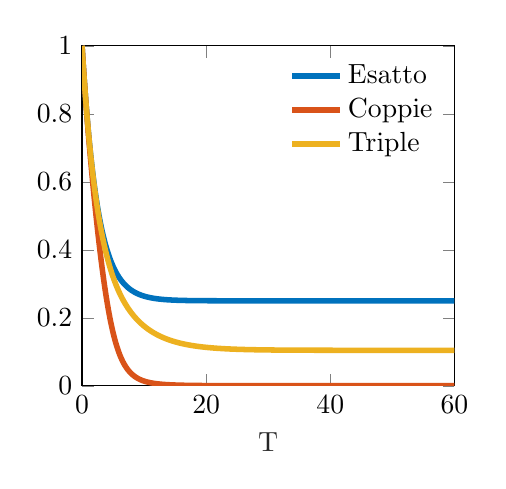
\begin{tikzpicture}

\begin{axis}[%
width=0.39\columnwidth,
height=1.7in,
at={(1.011in,0.642in)},
scale only axis,
xmin=0,
xmax=60,
xlabel style={font=\color{white!15!black}},
xlabel={T},
ymin=0,
ymax=1,
axis background/.style={fill=white},
legend style={legend cell align=left, align=left, draw=none,fill=none}
]
\addplot [color=mycolor1, line width=2.0pt]
  table[row sep=crcr]{%
0	1\\
0.00199053585276749	0.999403076915065\\
0.00398107170553497	0.99880662891969\\
0.00597160755830246	0.998210655635751\\
0.00796214341106994	0.997615156685427\\
0.0123567669950473	0.996302116207541\\
0.0167513905790247	0.994991381829635\\
0.0211460141630021	0.993682949501498\\
0.0255406377469794	0.992376815180021\\
0.0299388563931551	0.991071909148586\\
0.0343370750393307	0.98976929680375\\
0.0387352936855064	0.988468974113811\\
0.043133512331682	0.987170937054141\\
0.0475471725191068	0.985870636402437\\
0.0519608327065316	0.984572629359586\\
0.0563744928939564	0.983276911879878\\
0.0607881530813811	0.981983479924731\\
0.0652173199794049	0.980687797222947\\
0.0696464868774286	0.979394408006894\\
0.0740756537754524	0.978103308216878\\
0.0785048206734761	0.976814493800384\\
0.0829496187548012	0.975523424382033\\
0.0873944168361263	0.974234648341511\\
0.0918392149174515	0.972948161605001\\
0.0962840129987766	0.971663960105916\\
0.100744568101794	0.970377499369028\\
0.105205123204811	0.969093331917271\\
0.109665678307829	0.967811453662568\\
0.114126233410846	0.966531860524116\\
0.118602673075784	0.965250003840761\\
0.123079112740721	0.963970440365356\\
0.127555552405659	0.962693165995415\\
0.132031992070596	0.961418176635782\\
0.136524445545197	0.96014091935945\\
0.141016899019798	0.958865955229688\\
0.1455093524944	0.957593280129459\\
0.150001805969001	0.956322889949105\\
0.154510404254387	0.95505022741064\\
0.159019002539772	0.953779857973477\\
0.163527600825158	0.952511777505877\\
0.168036199110544	0.951245981883536\\
0.172561074936287	0.949977909407276\\
0.17708595076203	0.948712130003415\\
0.181610826587773	0.947448639525366\\
0.186135702413515	0.946187433834024\\
0.190676990405524	0.944923946699856\\
0.195218278397533	0.943662752625951\\
0.199759566389542	0.942403847450715\\
0.204300854381551	0.941147227020095\\
0.208858690959197	0.939888320502083\\
0.213416527536843	0.938631707049226\\
0.217974364114488	0.937377382484769\\
0.222532200692134	0.936125342639555\\
0.227106724202768	0.934871011978091\\
0.231681247713401	0.933618974404074\\
0.236255771224035	0.932369225725431\\
0.240830294734669	0.931121761757742\\
0.245421645441331	0.929872002173053\\
0.250012996147992	0.928624535715834\\
0.254604346854654	0.927379358178531\\
0.259195697561315	0.926136465361301\\
0.263804017673384	0.924891272055018\\
0.268412337785452	0.923648371934286\\
0.273020657897521	0.922407760775907\\
0.27762897800959	0.921169434364452\\
0.282254411746462	0.919928802512489\\
0.286879845483334	0.918690463922578\\
0.291505279220206	0.917454414355713\\
0.296130712957079	0.916220649580711\\
0.300773406613671	0.914984574326216\\
0.305416100270264	0.913750792429091\\
0.310058793926856	0.91251929963435\\
0.314701487583449	0.911290091694889\\
0.319361589521735	0.910058568161286\\
0.324021691460022	0.908829338099542\\
0.328681793398309	0.907602397238518\\
0.333341895336596	0.906377741315017\\
0.338019556071109	0.905150764594112\\
0.342697216805623	0.903926081479131\\
0.347374877540136	0.902703687682606\\
0.35205253827465	0.901483578925072\\
0.356747910447269	0.900261144094741\\
0.361443282619888	0.899041003024322\\
0.366138654792507	0.897823151409839\\
0.370834026965126	0.89660758495538\\
0.375547265516765	0.895389687045908\\
0.380260504068404	0.894174083070739\\
0.384973742620042	0.892960768709208\\
0.389686981171681	0.891749739648774\\
0.394418243246227	0.890536373679574\\
0.399149505320772	0.889325301839824\\
0.403880767395317	0.888116519791982\\
0.408612029469863	0.886910023206696\\
0.41336147459102	0.88570118415228\\
0.418110919712177	0.884494639443703\\
0.422860364833334	0.883290384726359\\
0.427609809954491	0.882088415653895\\
0.432377599961091	0.880884098472614\\
0.437145389967691	0.879682075875191\\
0.44191317997429	0.878482343489762\\
0.44668096998089	0.877284896952781\\
0.451467269141767	0.8760850965696\\
0.456253568302644	0.874887591030386\\
0.461039867463521	0.873692375945823\\
0.465826166624398	0.872499446934976\\
0.47063114173014	0.871304158231073\\
0.475436116835881	0.870111164653849\\
0.480241091941623	0.868920461796332\\
0.485046067047365	0.867732045260003\\
0.489869887370685	0.866541263095569\\
0.494693707694006	0.865352776363558\\
0.499517528017326	0.864166580639143\\
0.504341348340647	0.862982671506013\\
0.509184185682064	0.861796390721458\\
0.51402702302348	0.860612405698541\\
0.518869860364897	0.85943071199437\\
0.523712697706314	0.85825130517464\\
0.528574726619363	0.857069520548462\\
0.533436755532412	0.855890032037217\\
0.53829878444546	0.854712835179739\\
0.543160813358509	0.853537925523513\\
0.548042211039569	0.852360631813266\\
0.55292360872063	0.851185634595789\\
0.55780500640169	0.850012929391423\\
0.56268640408275	0.848842511729234\\
0.56758735048985	0.847669703656219\\
0.572488296896949	0.846499192478884\\
0.577389243304049	0.845330973698859\\
0.582290189711149	0.844165042826571\\
0.587210867601438	0.842996715080881\\
0.592131545491728	0.841830684659379\\
0.597052223382018	0.840666947044757\\
0.601972901272307	0.839505497728579\\
0.606913496388328	0.838341644939263\\
0.611854091504349	0.837180089928886\\
0.61679468662037	0.83602082816098\\
0.621735281736391	0.834863855108015\\
0.626695982628195	0.833704471900034\\
0.631656683519999	0.832547386952431\\
0.636617384411802	0.831392595709341\\
0.641578085303606	0.830240093623912\\
0.646559083672327	0.829085174552038\\
0.651540082041047	0.827932554249379\\
0.656521080409768	0.826782228140433\\
0.661502078778488	0.825634191658792\\
0.666503569383853	0.824483731245207\\
0.671505059989219	0.823335570137648\\
0.676506550594584	0.822189703740735\\
0.68150804119995	0.821046127468257\\
0.686530221876942	0.819900120213929\\
0.691552402553934	0.818756412830954\\
0.696574583230927	0.817615000703826\\
0.701596763907919	0.816475879226286\\
0.706639835866396	0.815334319558221\\
0.711682907824873	0.814195060356118\\
0.71672597978335	0.813058096984091\\
0.721769051741827	0.811923424815586\\
0.72683321952555	0.810786307113427\\
0.731897387309272	0.809651490501798\\
0.736961555092995	0.808518970324178\\
0.742025722876718	0.807388741933452\\
0.747111194287107	0.806256060563139\\
0.752196665697496	0.805125680938434\\
0.757282137107885	0.803997598381917\\
0.762367608518274	0.802871808225657\\
0.767474594900923	0.801743557491843\\
0.772581581283573	0.800617609189988\\
0.777688567666222	0.799493958621503\\
0.782795554048871	0.79837260109737\\
0.78792427039055	0.797248775240084\\
0.793052986732229	0.796127252533169\\
0.798181703073909	0.795008028256591\\
0.803310419415588	0.793891097699975\\
0.808461084325784	0.79277169091702\\
0.81361174923598	0.791654588035624\\
0.818762414146177	0.790539784314029\\
0.823913079056373	0.78942727502022\\
0.82908591482452	0.788312281472701\\
0.834258750592667	0.787199592611413\\
0.839431586360813	0.786089203672586\\
0.84460442212896	0.78498110990228\\
0.849799655005291	0.783870523672608\\
0.854994887881621	0.782762242948221\\
0.860190120757951	0.781656262943043\\
0.865385353634282	0.780552578880919\\
0.870603213699137	0.779446394020574\\
0.875821073763992	0.778342515519666\\
0.881038933828848	0.777240938569518\\
0.886256793893703	0.776141658371459\\
0.891497515445601	0.775039868838008\\
0.896738236997499	0.773940386554247\\
0.901978958549397	0.772843206688587\\
0.907219680101295	0.771748324419538\\
0.912483501408722	0.770650924149858\\
0.917747322716149	0.769555832056932\\
0.923011144023576	0.768463043285948\\
0.928274965331004	0.767372552992285\\
0.933562128954513	0.766279535854964\\
0.938849292578023	0.765188827859204\\
0.944136456201532	0.764100424126648\\
0.949423619825042	0.763014319789227\\
0.954734372782572	0.761925679572027\\
0.960045125740102	0.760839349499943\\
0.965355878697632	0.759755324670744\\
0.970666631655162	0.758673600192586\\
0.976001225418392	0.757589330625482\\
0.981335819181621	0.756507372246725\\
0.98667041294485	0.755427720129876\\
0.99200500670808	0.754350369358983\\
0.997363697280812	0.753270464120191\\
1.00272238785355	0.752192871153578\\
1.00808107842628	0.751117585508157\\
1.01343976899901	0.750044602243524\\
1.0188228172289	0.748969054919302\\
1.02420586545878	0.747895820992813\\
1.02958891368867	0.746824895488169\\
1.03497196191855	0.745756273440167\\
1.04037963341625	0.744685077565029\\
1.04578730491395	0.743616196255872\\
1.05119497641164	0.742549624511548\\
1.05660264790934	0.741485357341696\\
1.06203521338424	0.740418506355579\\
1.06746777885913	0.739353971147567\\
1.07290034433402	0.738291746690882\\
1.07833290980891	0.737231827969641\\
1.08379064506731	0.736169315243641\\
1.08924838032571	0.73510911955284\\
1.09470611558411	0.734051235844455\\
1.10016385084252	0.732995659076704\\
1.1056470369148	0.731937477913404\\
1.11113022298707	0.73088161508849\\
1.11661340905935	0.729828065522789\\
1.12209659513163	0.728776824148234\\
1.12760551858231	0.727722967747833\\
1.13311444203298	0.726671431036395\\
1.13862336548365	0.72562220890796\\
1.14413228893432	0.724575296267786\\
1.14966724184116	0.723525757759495\\
1.15520219474799	0.722478540339326\\
1.16073714765482	0.721433638874125\\
1.16627210056166	0.720391048242067\\
1.17183338076584	0.719345820663843\\
1.17739466097002	0.718302915622786\\
1.18295594117419	0.717262327958133\\
1.18851722137837	0.716224052520569\\
1.19410513262804	0.715183128820598\\
1.19969304387772	0.714144529158065\\
1.20528095512739	0.713108248344169\\
1.21086886637706	0.712074281201677\\
1.21648371859449	0.711037654217911\\
1.22209857081192	0.710003352824532\\
1.22771342302936	0.708971371804268\\
1.23332827524679	0.707941705951532\\
1.23897038457538	0.706909368433481\\
1.24461249390397	0.705879358112844\\
1.25025460323256	0.704851669743429\\
1.25589671256115	0.703826298090849\\
1.26156640151281	0.70279824270302\\
1.26723609046446	0.701772516175127\\
1.27290577941612	0.700749113231595\\
1.27857546836778	0.699728028608781\\
1.28427306633634	0.698704247869228\\
1.28997066430491	0.697682797709356\\
1.29566826227347	0.696663672823736\\
1.30136586024204	0.695646867918998\\
1.30709170327692	0.694627354273799\\
1.31281754631181	0.693610172986684\\
1.31854338934669	0.692595318721888\\
1.32426923238158	0.691582786155827\\
1.33002366371043	0.690567531918648\\
1.33577809503928	0.689554611878364\\
1.34153252636813	0.688544020668372\\
1.34728695769699	0.687535752934384\\
1.35307032782915	0.686524750303618\\
1.35885369796131	0.685516083770681\\
1.36463706809348	0.684509747937618\\
1.37042043822564	0.683505737418925\\
1.37622881553645	0.682499720580793\\
1.38203719284726	0.681496038359702\\
1.38784557015807	0.680494685337819\\
1.39365394746888	0.679495656109863\\
1.39948194569202	0.678495582280198\\
1.40530994391516	0.677497837106605\\
1.41113794213829	0.676502415166854\\
1.41696594036143	0.675509311051313\\
1.4228137248248	0.674515159526085\\
1.42866150928816	0.673523330716793\\
1.43450929375153	0.672533819196698\\
1.44035707821489	0.671546619551714\\
1.44622478964653	0.670558374185696\\
1.45209250107816	0.669572445595239\\
1.45796021250979	0.66858882834906\\
1.46382792394143	0.667607517028582\\
1.46971570462452	0.666625161672456\\
1.4756034853076	0.665645117151287\\
1.48149126599069	0.66466737802921\\
1.48737904667378	0.663691938883123\\
1.49328704060906	0.662715457360543\\
1.49919503454433	0.661741280732202\\
1.50510302847961	0.660769403557618\\
1.51101102241489	0.659799820409127\\
1.51693937480906	0.658829196605364\\
1.52286772720322	0.65786087175471\\
1.52879607959739	0.65689484041203\\
1.53472443199155	0.65593109714506\\
1.540673290528	0.654966314802033\\
1.54662214906446	0.654003825471241\\
1.55257100760091	0.653043623702855\\
1.55851986613736	0.652085704059977\\
1.56448937947106	0.651126747028285\\
1.57045889280476	0.650170077067689\\
1.57642840613847	0.649215688723629\\
1.58239791947216	0.648263576554532\\
1.58838823791446	0.647310428683399\\
1.59437855635675	0.646359561941951\\
1.60036887479904	0.645410970870862\\
1.60635919324133	0.644464650023846\\
1.61237046959671	0.643517295033318\\
1.61838174595208	0.642572215231405\\
1.62439302230746	0.641629405153972\\
1.63040429866284	0.640688859349981\\
1.63643668672632	0.639747281075257\\
1.6424690747898	0.638807972047861\\
1.64850146285328	0.63787092679881\\
1.65453385091676	0.636936139872275\\
1.66058750665404	0.636000322080035\\
1.66664116239132	0.63506676759394\\
1.67269481812859	0.634135470940117\\
1.67874847386587	0.633206426657907\\
1.68482355500326	0.632276353116294\\
1.69089863614064	0.631348536939732\\
1.69697371727803	0.630422972649421\\
1.70304879841541	0.629499654779829\\
1.70914546464501	0.628575309231395\\
1.71524213087462	0.627653215107132\\
1.72133879710422	0.626733366923264\\
1.72743546333383	0.625815759209347\\
1.73355387572031	0.624897125465399\\
1.73967228810678	0.623980737204609\\
1.74579070049326	0.62306658893819\\
1.75190911287974	0.622154675190741\\
1.75804943463327	0.621241737017398\\
1.76418975638681	0.620331038386286\\
1.77033007814035	0.619422573803557\\
1.77647039989388	0.618516337788816\\
1.78263279664118	0.617609078873531\\
1.78879519338848	0.61670405356001\\
1.79495759013578	0.615801256349305\\
1.80111998688309	0.61490068175598\\
1.80730462566597	0.61399908586145\\
1.81348926444885	0.613099717628309\\
1.81967390323173	0.612202571552465\\
1.82585854201462	0.611307642143397\\
1.83206559217232	0.610411692981052\\
1.83827264233002	0.609517965540063\\
1.84447969248772	0.608626454311144\\
1.85068674264543	0.607737153798647\\
1.85691637550678	0.606846835079462\\
1.86314600836813	0.605958732141937\\
1.86937564122948	0.605072839471552\\
1.87560527409083	0.604189151567482\\
1.88185766319929	0.603304446974639\\
1.88811005230775	0.602421952224236\\
1.89436244141622	0.601541661796471\\
1.90061483052468	0.600663570185298\\
1.90689015093446	0.599784463478542\\
1.91316547134424	0.5989075606751\\
1.91944079175402	0.598032856249839\\
1.92571611216381	0.597160344691447\\
1.93201454150218	0.596286819560686\\
1.93831297084055	0.595415492394549\\
1.94461140017892	0.594546357662525\\
1.9509098295173	0.593679409847991\\
1.95723154808653	0.592811449907329\\
1.96355326665576	0.591945681993422\\
1.96987498522499	0.59108210057033\\
1.97619670379422	0.590220700116066\\
1.98254189319299	0.589358289099411\\
1.98888708259176	0.588498064171857\\
1.99523227199053	0.587640019791989\\
2.0015774613893	0.586784150432407\\
2.00794630624256	0.585927271959772\\
2.01431515109582	0.585072573639376\\
2.02068399594908	0.584220049924275\\
2.02705284080234	0.583369695281611\\
2.03344552746868	0.582518333041505\\
2.03983821413503	0.581669145017222\\
2.04623090080137	0.580822125656242\\
2.05262358746771	0.579977269420194\\
2.05904030495676	0.579131407050252\\
2.06545702244581	0.578287712960424\\
2.07187373993486	0.57744618159256\\
2.07829045742391	0.576606807402726\\
2.084731396657	0.575766428593491\\
2.0911723358901	0.574928212129099\\
2.0976132751232	0.574092152445717\\
2.1040542143563	0.573258243993798\\
2.11051956957009	0.572423332309956\\
2.11698492478388	0.571590577036772\\
2.12345027999767	0.570759972604675\\
2.12991563521146	0.569931513458451\\
2.13640560238783	0.569102052550658\\
2.1428955695642	0.568274742119988\\
2.14938553674057	0.567449576591077\\
2.15587550391694	0.566626550402991\\
2.16239028199053	0.565802523856075\\
2.16890506006412	0.564980641853739\\
2.17541983813771	0.564160898814776\\
2.1819346162113	0.563343289172471\\
2.18847440630977	0.562524680608923\\
2.19501419640825	0.561708210658219\\
2.20155398650673	0.560893873733249\\
2.20809377660521	0.560081664261466\\
2.21465878275268	0.559268457257725\\
2.22122378890015	0.558457382936144\\
2.22778879504762	0.557648435703651\\
2.23435380119508	0.556841609981812\\
2.24094422983074	0.556033788134853\\
2.24753465846639	0.555228093040322\\
2.25412508710205	0.554424519099128\\
2.2607155157377	0.55362306072689\\
2.2673315759421	0.552820607631124\\
2.27394763614649	0.552020275359027\\
2.28056369635089	0.55122205830543\\
2.28717975655528	0.550425950879947\\
2.29382166035897	0.54962885009578\\
2.30046356416266	0.548833864207683\\
2.30710546796636	0.548040987604348\\
2.31374737177005	0.547250214689325\\
2.32041533418655	0.546458449746524\\
2.32708329660306	0.545668793773527\\
2.33375125901957	0.544881241152828\\
2.34041922143607	0.544095786281849\\
2.34711345989709	0.54330934075302\\
2.3538076983581	0.542524998268848\\
2.36050193681912	0.541742753205565\\
2.36719617528013	0.540962599954407\\
2.37391691043736	0.540181457365341\\
2.3806376455946	0.539402411897166\\
2.38735838075183	0.538625457919786\\
2.39407911590907	0.537850589818188\\
2.40082657131283	0.537074733692972\\
2.40757402671659	0.536300968766284\\
2.41432148212035	0.535529289401637\\
2.42106893752412	0.534759689977702\\
2.42784333963791	0.533989103842992\\
2.4346177417517	0.533220602985851\\
2.4413921438655	0.532454181763332\\
2.44816654597929	0.531689834547729\\
2.4549681243632	0.530924501917909\\
2.4617697027471	0.530161248646181\\
2.46857128113101	0.529400069083077\\
2.47537285951492	0.528640957594445\\
2.48220184698832	0.527880861960174\\
2.48903083446173	0.52712283976615\\
2.49585982193513	0.526366885356312\\
2.50268880940853	0.525612993089997\\
2.50954544177924	0.524858117955344\\
2.51640207414995	0.524105310344667\\
2.52325870652066	0.523354564595246\\
2.53011533889137	0.522605875059835\\
2.53699985562036	0.521856203875431\\
2.54388437234935	0.52110859430062\\
2.55076888907833	0.52036304066595\\
2.55765340580732	0.519619537317522\\
2.5645660494942	0.518875053545048\\
2.57147869318108	0.518132625469634\\
2.57839133686796	0.517392247415021\\
2.58530398055484	0.516653913720589\\
2.59224499685821	0.515914600847029\\
2.59918601316159	0.515177337759725\\
2.60612702946496	0.514442118775542\\
2.61306804576833	0.513708938227065\\
2.62003768421203	0.512974779684941\\
2.62700732265572	0.512242665020325\\
2.63397696109942	0.511512588543128\\
2.64094659954311	0.510784544579069\\
2.64794511298781	0.51005552381091\\
2.65494362643251	0.509328541013536\\
2.6619421398772	0.50860359048983\\
2.6689406533219	0.507880666558564\\
2.67596829852112	0.507156766965813\\
2.68299594372033	0.506434899439404\\
2.69002358891955	0.505715058275114\\
2.69705123411877	0.504997237784695\\
2.70410827073433	0.504278442836862\\
2.71116530734989	0.503561674052857\\
2.71822234396545	0.502846925721273\\
2.72527938058101	0.502134192146763\\
2.73236607296869	0.501420485204902\\
2.73945276535637	0.500708798526921\\
2.74653945774405	0.499999126394145\\
2.75362615013173	0.499291463104051\\
2.76074276611797	0.498582827555353\\
2.76785938210422	0.497876206373041\\
2.77497599809046	0.497171593831091\\
2.78209261407671	0.496468984219718\\
2.78923942490227	0.495765403488699\\
2.79638623572783	0.495063831228844\\
2.80353304655339	0.494364261706698\\
2.81067985737896	0.493666689205136\\
2.81785713902212	0.492968146630075\\
2.82503442066529	0.492271606633755\\
2.83221170230846	0.491577063475205\\
2.83938898395163	0.490884511429871\\
2.84659701614953	0.490190990368968\\
2.85380504834743	0.489499465997106\\
2.86101308054533	0.488809932565711\\
2.86822111274323	0.488122384342717\\
2.87546017926332	0.487433868154604\\
2.88269924578341	0.486747342768596\\
2.88993831230351	0.486062802428422\\
2.8971773788236	0.48538024139442\\
2.90444776780364	0.484696713413736\\
2.91171815678368	0.484015170351159\\
2.91898854576373	0.483335606442635\\
2.92625893474377	0.482658015940809\\
2.93356093845992	0.481979459508713\\
2.94086294217606	0.48130288211367\\
2.94816494589221	0.48062827798375\\
2.95546694960836	0.479955641363819\\
2.96280086487659	0.479282039798549\\
2.97013478014483	0.4786104113924\\
2.97746869541306	0.477940750365474\\
2.9848026106813	0.477273050954764\\
2.99216873909201	0.476604387539565\\
2.99953486750271	0.475937691408931\\
3.00690099591342	0.475272956774899\\
3.01426712432413	0.474610177866491\\
3.02166577186631	0.47394643589333\\
3.02906441940849	0.473284655333555\\
3.03646306695067	0.472624830391036\\
3.04386171449286	0.471966955286733\\
3.05129319192691	0.471308118030965\\
3.05872466936097	0.470651236320929\\
3.06615614679503	0.469996304352233\\
3.07358762422909	0.469343316337668\\
3.08105224696524	0.468689367077934\\
3.0885168697014	0.46803736749984\\
3.09598149243755	0.467387311790626\\
3.1034461151737	0.466739194154822\\
3.11094420406679	0.466090116112579\\
3.11844229295988	0.465442981891844\\
3.12594038185297	0.464797785671387\\
3.13343847074605	0.464154521647367\\
3.14097035080817	0.463510298108793\\
3.14850223087028	0.462868012535231\\
3.1560341109324	0.462227659096873\\
3.16356599099451	0.461589231981405\\
3.17113199342146	0.460949846131304\\
3.17869799584842	0.460312392394024\\
3.18626399827537	0.459676864931069\\
3.19383000070233	0.459043257921544\\
3.20143046110215	0.458408693005911\\
3.20903092150198	0.457776054354912\\
3.21663138190181	0.457145336121254\\
3.22423184230164	0.45651653247535\\
3.2318671021242	0.455886771689044\\
3.23950236194676	0.455258931323566\\
3.24713762176933	0.454633005522714\\
3.25477288159189	0.454008988448097\\
3.26244328804483	0.453384014953912\\
3.27011369449776	0.452760956041404\\
3.2777841009507	0.452139805845339\\
3.28545450740363	0.451520558518409\\
3.29316041266953	0.45090035552131\\
3.30086631793543	0.450282061271204\\
3.30857222320133	0.449665669893713\\
3.31627812846722	0.449051175532496\\
3.32401989110489	0.448435726175378\\
3.33176165374256	0.447822179735501\\
3.33950341638023	0.44721053032922\\
3.3472451790179	0.446600772091036\\
3.35502316313618	0.445990059532961\\
3.36280114725446	0.445381244067288\\
3.37057913137275	0.444774319800982\\
3.37835711549103	0.444169280859267\\
3.38617169154667	0.443563288222598\\
3.3939862676023	0.442959186858721\\
3.40180084365794	0.442356970865085\\
3.40961541971357	0.44175663435751\\
3.41746696420648	0.441155344763534\\
3.42531850869938	0.44055594062807\\
3.43317005319229	0.439958416038915\\
3.4410215976852	0.439362765102361\\
3.44891049346576	0.438766161658431\\
3.45679938924632	0.438171437864239\\
3.46468828502688	0.437578587797804\\
3.47257718080744	0.436987605555755\\
3.48050381756295	0.436395671330335\\
3.48843045431847	0.435805610951734\\
3.49635709107398	0.435217418488053\\
3.50428372782949	0.434631088026126\\
3.51224850159594	0.434043806097833\\
3.52021327536239	0.433458392219333\\
3.52817804912884	0.432874840448674\\
3.53614282289529	0.432293144862755\\
3.54414613607264	0.431710498329503\\
3.55214944924998	0.431129714054896\\
3.56015276242733	0.430550786086788\\
3.56815607560468	0.429973708492006\\
3.57619833889781	0.42939568034156\\
3.58424060219095	0.428819508665307\\
3.59228286548408	0.428245187500755\\
3.60032512877721	0.427672710904515\\
3.60840675922679	0.427099284172238\\
3.61648838967638	0.42652770813621\\
3.62457002012596	0.42595797682345\\
3.63265165057554	0.425390084280203\\
3.64077307248204	0.424821241993017\\
3.64889449438855	0.424254244630826\\
3.65701591629505	0.423689086210002\\
3.66513733820155	0.423125760766277\\
3.67329898353354	0.422561485926762\\
3.68146062886554	0.421999050247955\\
3.68962227419754	0.421438447735434\\
3.69778391952953	0.420879672414258\\
3.70598622860803	0.42031994796756\\
3.71418853768653	0.419762056924767\\
3.72239084676502	0.419205993280494\\
3.73059315584352	0.418651751048974\\
3.73883657626523	0.418096559971174\\
3.74707999668693	0.417543196547895\\
3.75532341710863	0.416991654762629\\
3.76356683753034	0.416441928618619\\
3.77185182516863	0.415891253860852\\
3.78013681280692	0.41534240101595\\
3.78842180044522	0.414795364056115\\
3.79670678808351	0.414250136973437\\
3.80503380745825	0.41370396145204\\
3.81336082683299	0.413159602109966\\
3.82168784620774	0.412617052907952\\
3.83001486558248	0.412076307826761\\
3.83838438958511	0.411534614456356\\
3.84675391358775	0.410994731540014\\
3.85512343759039	0.41045665302683\\
3.86349296159302	0.40992037288607\\
3.8719054722877	0.409383144541932\\
3.88031798298237	0.408847720935309\\
3.88873049367705	0.408314096003473\\
3.89714300437172	0.407782263704011\\
3.90559899284027	0.407249483248037\\
3.91405498130882	0.406718501822005\\
3.92251096977737	0.406189313351181\\
3.93096695824593	0.405661911781289\\
3.93946692479213	0.405133562064155\\
3.94796689133833	0.404607005678626\\
3.95646685788454	0.404082236537769\\
3.96496682443074	0.403559248575256\\
3.97351127881372	0.403035312437119\\
3.98205573319669	0.402513163941744\\
3.99060018757967	0.401992796989805\\
3.99914464196265	0.40147420550273\\
4.00773410425464	0.400954665736679\\
4.01632356654662	0.40043690793456\\
4.02491302883861	0.399920925984454\\
4.0335024911306	0.399406713795342\\
4.04213749081375	0.398891553219244\\
4.05077249049689	0.398378168938299\\
4.05940749018004	0.397866554827785\\
4.06804248986318	0.397356704784042\\
4.07672356764034	0.396845906147724\\
4.08540464541749	0.39633687814851\\
4.09408572319465	0.395829614648669\\
4.10276680097181	0.395324109531682\\
4.11149450824228	0.394817655567482\\
4.12022221551276	0.394312966593421\\
4.12894992278323	0.393810036458534\\
4.1376776300537	0.393308859033232\\
4.14645252883691	0.39280673247755\\
4.15522742762012	0.392306365276329\\
4.16400232640333	0.391807751265149\\
4.17277722518654	0.391310884301129\\
4.18159988926615	0.390813067846041\\
4.19042255334575	0.390317005121578\\
4.19924521742536	0.389822689949636\\
4.20806788150496	0.389330116173814\\
4.21693889629988	0.388836592494013\\
4.22580991109479	0.388344816933222\\
4.23468092588971	0.387854783299419\\
4.24355194068463	0.38736648542245\\
4.2524719033702	0.386877237186965\\
4.26139186605577	0.386389731471409\\
4.27031182874135	0.385903962069595\\
4.27923179142692	0.385419922797375\\
4.28820131218307	0.384934932620153\\
4.29717083293922	0.384451679376977\\
4.30614035369538	0.383970156847247\\
4.31510987445153	0.383490358832575\\
4.32412957614907	0.383009609311017\\
4.33314927784661	0.382530591151236\\
4.34216897954416	0.38205329811796\\
4.3511886812417	0.381577723998309\\
4.36025919971018	0.381101197718879\\
4.36932971817866	0.380626397242954\\
4.37840023664715	0.380153316320329\\
4.38747075511563	0.379681948723365\\
4.39659274002011	0.379209628235977\\
4.40571472492458	0.378739028008404\\
4.41483670982906	0.378270141775232\\
4.42395869473353	0.377802963293798\\
4.43313280988389	0.377334831118071\\
4.44230692503424	0.376868413673604\\
4.45148104018459	0.376403704679494\\
4.46065515533495	0.375940697877775\\
4.469882079136	0.37547673650255\\
4.47910900293706	0.375014484345741\\
4.48833592673811	0.374553935110665\\
4.49756285053916	0.374095082523766\\
4.50684327607396	0.373635274425678\\
4.51612370160877	0.373177170049325\\
4.52540412714357	0.372720763081951\\
4.53468455267837	0.372266047234115\\
4.54401918924822	0.371810374824447\\
4.55335382581807	0.371356400656866\\
4.56268846238792	0.37090411840223\\
4.57202309895777	0.370453521754911\\
4.58141267108196	0.370001967453971\\
4.59080224320616	0.369552105932836\\
4.60019181533036	0.369103930845661\\
4.60958138745456	0.368657435870321\\
4.61902663678989	0.368209982038221\\
4.62847188612523	0.367764215541877\\
4.63791713546056	0.367320130018416\\
4.6473623847959	0.366877719128887\\
4.65686406984621	0.366434348106303\\
4.66636575489653	0.365992658994244\\
4.67586743994685	0.365552645412473\\
4.68536912499717	0.365114301004881\\
4.69492802222378	0.364674995087027\\
4.7044869194504	0.364237365674092\\
4.71404581667701	0.363801406368124\\
4.72360471390363	0.36336711079551\\
4.73320764525141	0.362932483436382\\
4.74281057659919	0.362499522353675\\
4.75241350794698	0.362068221159235\\
4.76201643929476	0.361638573489322\\
4.77165794452804	0.361208857088269\\
4.78129944976131	0.360780794740846\\
4.79094095499459	0.360354380080335\\
4.80058246022786	0.359929606764447\\
4.81026314694842	0.359504752238238\\
4.81994383366897	0.359081539684343\\
4.82962452038952	0.358659962756912\\
4.83930520711008	0.358240015134544\\
4.84902565638322	0.357819975627652\\
4.85874610565637	0.357401566138915\\
4.86846655492951	0.356984780342857\\
4.87818700420266	0.356569611938475\\
4.88794780523678	0.356154341229547\\
4.89770860627089	0.355740688709528\\
4.90746940730501	0.35532864807283\\
4.91723020833913	0.354918213038361\\
4.92703195872998	0.354507665526815\\
4.93683370912084	0.354098724497657\\
4.9466354595117	0.353691383664708\\
4.95643720990256	0.353285636766306\\
4.96628051524823	0.352879767485449\\
4.97612382059389	0.352475493100847\\
4.98596712593956	0.352072807345252\\
4.99581043128522	0.351671703975962\\
5.00569590732134	0.351270468502172\\
5.01558138335745	0.350870816457215\\
5.02546685939356	0.3504727415923\\
5.03535233542967	0.350076237683216\\
5.04528060635073	0.349679592205041\\
5.05520887727179	0.349284518804724\\
5.06513714819285	0.348891011251467\\
5.07506541911391	0.348499063339085\\
5.08503711889176	0.348106964601862\\
5.0950088186696	0.347716426706099\\
5.10498051844744	0.347327443438525\\
5.11495221822528	0.34694000861052\\
5.12496799094167	0.346552413903657\\
5.13498376365806	0.346166368914615\\
5.14499953637444	0.345781867447191\\
5.15501530909083	0.345398903329876\\
5.16507580953502	0.345015770464823\\
5.17513630997921	0.34463417630503\\
5.18519681042339	0.344254114670907\\
5.19525731086758	0.343875579407601\\
5.2053632039849	0.343496866740483\\
5.21546909710223	0.34311968187524\\
5.22557499021955	0.342744018648443\\
5.23568088333688	0.342369870921446\\
5.24583284576096	0.341995537296497\\
5.25598480818505	0.341622720677726\\
5.26613677060914	0.341251414917413\\
5.27628873303322	0.340881613892671\\
5.28648745229033	0.340511618674941\\
5.29668617154743	0.340143129773586\\
5.30688489080453	0.339776141056149\\
5.31708361006163	0.33941064641506\\
5.32732978639303	0.339044949426455\\
5.33757596272443	0.338680748169006\\
5.34782213905582	0.338318036525074\\
5.35806831538722	0.337956808401959\\
5.36836266133408	0.337595369941506\\
5.37865700728095	0.337235416730064\\
5.38895135322782	0.336876942664367\\
5.39924569917468	0.336519941666145\\
5.40958894010065	0.336162722495822\\
5.41993218102661	0.335806978194011\\
5.43027542195257	0.335452702671376\\
5.44061866287853	0.335099889863637\\
5.45101153706255	0.334746851209919\\
5.46140441124658	0.334395277144383\\
5.4717972854306	0.334045161591181\\
5.48219015961463	0.333696498499587\\
5.49263341945276	0.33334760201767\\
5.50307667929089	0.333000159942559\\
5.51351993912902	0.332654166211454\\
5.52396319896715	0.332309614786741\\
5.53445761187213	0.331964822538001\\
5.54495202477712	0.331621474612589\\
5.5554464376821	0.331279564960309\\
5.56594085058709	0.330939087556223\\
5.57648719831941	0.330598362038436\\
5.58703354605173	0.330259070857061\\
5.59757989378405	0.329921207974064\\
5.60812624151637	0.329584767376746\\
5.61872532103302	0.329248071503203\\
5.62932440054967	0.328912800074524\\
5.63992348006633	0.328578947064399\\
5.65052255958298	0.328246506471925\\
5.66117518401188	0.327913803548608\\
5.67182780844078	0.327582515272947\\
5.68248043286967	0.327252635629912\\
5.69313305729857	0.326924158629958\\
5.70384005671797	0.326595412340964\\
5.71454705613736	0.326268070995831\\
5.72525405555675	0.325942128590359\\
5.73596105497615	0.325617579145922\\
5.74672327665992	0.325292753556537\\
5.75748549834369	0.324969323299646\\
5.76824772002746	0.324647282381439\\
5.77900994171123	0.324326624833759\\
5.78982825023888	0.32400568439736\\
5.80064655876654	0.323686129773457\\
5.81146486729419	0.323367954978178\\
5.82228317582184	0.323051154053395\\
5.83315845473553	0.322734063572754\\
5.84403373364921	0.322418349475224\\
5.8549090125629	0.322104005786419\\
5.86578429147658	0.321791026557792\\
5.87671744355088	0.321477751190118\\
5.88765059562518	0.321165842865966\\
5.89858374769948	0.320855295619981\\
5.90951689977378	0.320546103512745\\
5.92050884813521	0.320236608750612\\
5.93150079649664	0.319928471781536\\
5.94249274485807	0.319621686648736\\
5.9534846932195	0.319316247421468\\
5.96453638108293	0.319010499114169\\
5.97558806894636	0.318706099437712\\
5.98663975680979	0.318403042443427\\
5.99769144467322	0.318101322208788\\
6.00880383710542	0.317799286526827\\
6.01991622953761	0.317498590401161\\
6.0310286219698	0.317199227890766\\
6.042141014402	0.316901193080866\\
6.05331509935885	0.316602836503793\\
6.0644891843157	0.316305810495649\\
6.07566326927256	0.316010109122579\\
6.08683735422941	0.315715726477095\\
6.09807414230094	0.315421015816895\\
6.10931093037248	0.315127626824729\\
6.12054771844401	0.314835553573436\\
6.13178450651555	0.314544790162339\\
6.14308503319571	0.314253692519959\\
6.15438555987588	0.313963907730853\\
6.16568608655605	0.313675429874071\\
6.17698661323621	0.313388253055268\\
6.18835193888863	0.313100735840356\\
6.19971726454106	0.312814522749576\\
6.21108259019348	0.3125296078677\\
6.2224479158459	0.312245985306225\\
6.23387912710053	0.311962016219945\\
6.24531033835517	0.311679342613899\\
6.2567415496098	0.311397958578078\\
6.26817276086443	0.311117858229334\\
6.2796709718506	0.310837405253584\\
6.29116918283678	0.310558239199129\\
6.30266739382295	0.310280354160675\\
6.31416560480912	0.310003744259924\\
6.32573195844141	0.30972677564715\\
6.33729831207371	0.309451085481498\\
6.34886466570601	0.309176667861873\\
6.36043101933831	0.308903516914315\\
6.37206668825559	0.308630001187349\\
6.38370235717287	0.308357755517901\\
6.39533802609016	0.308086774008553\\
6.40697369500744	0.307817050789164\\
6.41867988207414	0.307546956752004\\
6.43038606914084	0.307278124467034\\
6.44209225620754	0.307010548039977\\
6.45379844327423	0.306744221603984\\
6.46557638449348	0.306477518297767\\
6.47735432571273	0.306212068522802\\
6.48913226693197	0.305947866387406\\
6.50091020815122	0.305684906027479\\
6.51276117329228	0.305421562742897\\
6.52461213843333	0.30515946485302\\
6.53646310357439	0.304898606468203\\
6.54831406871544	0.304638981726542\\
6.56023936237899	0.304378968006487\\
6.57216465604253	0.304120191628968\\
6.58408994970607	0.303862646705806\\
6.59601524336962	0.303606327376731\\
6.608016207688	0.303349612984866\\
6.62001717200638	0.303094127968035\\
6.63201813632476	0.302839866438942\\
6.64401910064313	0.302586822538372\\
6.65609711612489	0.302333377471268\\
6.66817513160664	0.302081153896556\\
6.68025314708839	0.301830145927221\\
6.69233116257014	0.30158034770451\\
6.70448764976455	0.301330142186955\\
6.71664413695897	0.301081150364253\\
6.72880062415338	0.300833366349061\\
6.7409571113478	0.300586784282478\\
6.75319353351478	0.30033978874444\\
6.76542995568177	0.300093999189314\\
6.77766637784875	0.299849409728791\\
6.78990280001574	0.299606014503198\\
6.80222066442117	0.299362199588071\\
6.8145385288266	0.299119583029937\\
6.82685639323203	0.298878158938876\\
6.83917425763746	0.2986379214538\\
6.85157511856051	0.298397257994209\\
6.86397597948357	0.298157785352412\\
6.87637684040662	0.297919497636206\\
6.88877770132968	0.297682388982423\\
6.90126316148383	0.297444848010683\\
6.91374862163799	0.297208490404876\\
6.92623408179214	0.296973310269827\\
6.93871954194629	0.296739301739609\\
6.95129125486549	0.296504854480924\\
6.96386296778468	0.296271583224374\\
6.97643468070388	0.296039482071097\\
6.98900639362307	0.295808545151699\\
7.00166606764739	0.295577162990967\\
7.0143257416717	0.295346949557721\\
7.02698541569601	0.295117898948676\\
7.03964508972033	0.294890005290242\\
7.05239448925109	0.294661659793715\\
7.06514388878186	0.294434475840095\\
7.07789328831262	0.294208447520913\\
7.09064268784339	0.293983568957626\\
7.10348363709426	0.293758231850704\\
7.11632458634514	0.293534049193375\\
7.12916553559601	0.29331101507119\\
7.14200648484689	0.293089123599873\\
7.15494087138423	0.292866766753613\\
7.16787525792157	0.292645557356277\\
7.18080964445891	0.29242548948662\\
7.19374403099625	0.292206557253819\\
7.20677380774895	0.291987152701476\\
7.21980358450165	0.291768888691319\\
7.23283336125435	0.291551759294449\\
7.24586313800706	0.291335758612658\\
7.25899032889946	0.291119278507525\\
7.27211751979186	0.290903932133548\\
7.28524471068426	0.290689713553289\\
7.29837190157667	0.290476616860272\\
7.31159860422458	0.290263033489001\\
7.32482530687249	0.290050577135289\\
7.3380520095204	0.289839241852236\\
7.35127871216831	0.289629021724182\\
7.36460710304072	0.289418307482998\\
7.37793549391314	0.28920871364527\\
7.39126388478556	0.289000234253667\\
7.40459227565797	0.288792863382394\\
7.41802461355885	0.288584990785761\\
7.43145695145972	0.288378232080037\\
7.4448892893606	0.288172581296454\\
7.45832162726148	0.287968032498085\\
7.47186025959003	0.287762974148193\\
7.48539889191859	0.287559023280717\\
7.49893752424715	0.287356173914392\\
7.51247615657571	0.287154420100116\\
7.52612352432791	0.286952148682948\\
7.53977089208011	0.286750978446408\\
7.55341825983232	0.286550903395634\\
7.56706562758452	0.286351917568252\\
7.58082427117841	0.286152405842785\\
7.5945829147723	0.285953989105771\\
7.60834155836619	0.285756661347589\\
7.62210020196009	0.285560416591451\\
7.63597276754062	0.285363637378323\\
7.64984533312116	0.285167947074264\\
7.66371789870169	0.284973339653673\\
7.67759046428223	0.284779809124137\\
7.69157971106386	0.284585735286684\\
7.70556895784549	0.284392744395248\\
7.71955820462712	0.284200830406965\\
7.73354745140875	0.284009987312529\\
7.7476562591015	0.283818591744841\\
7.76176506679424	0.283628273280311\\
7.77587387448699	0.283439025857455\\
7.78998268217974	0.283250843448738\\
7.80421406003167	0.283062099050118\\
7.81844543788359	0.282874426036333\\
7.83267681573552	0.282687818325848\\
7.84690819358745	0.282502269871487\\
7.86126528820976	0.282316149546761\\
7.87562238283208	0.28213109501765\\
7.8899794774544	0.281947100181056\\
7.90433657207672	0.281764158968666\\
7.91882267896367	0.281580635589139\\
7.93330878585062	0.281398172550365\\
7.94779489273757	0.281216763726081\\
7.96228099962452	0.28103640302525\\
7.97689957365268	0.280855449415443\\
7.99151814768085	0.280675550831578\\
8.00613672170902	0.280496701122521\\
8.02075529573718	0.28031889417283\\
8.03550996276884	0.28014048309451\\
8.0502646298005	0.279963121873554\\
8.06501929683216	0.279786804332147\\
8.07977396386382	0.279611524328652\\
8.09466853533245	0.279435628441472\\
8.10956310680107	0.2792607773963\\
8.12445767826969	0.279086964986711\\
8.13935224973832	0.278914185042966\\
8.15439073744049	0.278740776878611\\
8.16942922514267	0.278568408701819\\
8.18446771284484	0.278397074275494\\
8.19950620054702	0.278226767399757\\
8.2146928332504	0.278055819330898\\
8.22987946595378	0.277885906564567\\
8.24506609865717	0.277717022830785\\
8.26025273136055	0.277549161897355\\
8.27559197362809	0.277380646099422\\
8.29093121589562	0.277213161097839\\
8.30627045816316	0.277046700587381\\
8.32160970043069	0.276881258301191\\
8.33710627308224	0.276715146716129\\
8.35260284573378	0.27655006161055\\
8.36809941838533	0.276385996641432\\
8.38359599103687	0.276222945504748\\
8.39925489573158	0.276059209782584\\
8.41491380042629	0.275896496424141\\
8.430572705121	0.27573479904586\\
8.44623160981571	0.275574111303833\\
8.46205815432056	0.275412722763022\\
8.4778846988254	0.275252352684289\\
8.49371124333024	0.275092994640573\\
8.50953778783509	0.274934642245159\\
8.52553761739547	0.274775571797586\\
8.54153744695585	0.274617516139336\\
8.55753727651623	0.274460468796635\\
8.57353710607661	0.274304423336788\\
8.58971623619016	0.274147641431848\\
8.60589536630372	0.273991870888783\\
8.62207449641727	0.273837105183616\\
8.63825362653082	0.273683337834231\\
8.65461848330403	0.273528814364154\\
8.67098334007723	0.273375299092517\\
8.68734819685043	0.273222785441339\\
8.70371305362364	0.273071266875322\\
8.72018188980809	0.27291978360775\\
8.73665072599255	0.272769294961837\\
8.75311956217701	0.27261979440709\\
8.76958839836146	0.272471275455657\\
8.78614348346302	0.2723229615165\\
8.80269856856458	0.272175626472643\\
8.81925365366614	0.272029263863299\\
8.83580873876771	0.271883867270088\\
8.85245111606455	0.271738671257211\\
8.86909349336139	0.271594438597074\\
8.88573587065824	0.271451162898058\\
8.90237824795508	0.271308837810718\\
8.91910883699713	0.271166710153587\\
8.93583942603918	0.271025530472709\\
8.95257001508123	0.27088529244526\\
8.96930060412328	0.270745989790352\\
8.98612034063892	0.270606881435329\\
9.00294007715455	0.270468705845428\\
9.01975981367019	0.270331456766243\\
9.03657955018582	0.27019512798507\\
9.05348938408815	0.270058990412795\\
9.07039921799048	0.269923770558884\\
9.08730905189281	0.269789462236972\\
9.10421888579513	0.269656059302164\\
9.12121978296026	0.269522844512469\\
9.13822068012539	0.269390532557933\\
9.15522157729052	0.269259117319854\\
9.17222247445565	0.269128592720769\\
9.18931541587169	0.268998253239531\\
9.20640835728774	0.268868801872844\\
9.22350129870378	0.2687402325693\\
9.24059424011982	0.268612539318485\\
9.25778022278737	0.268485028190085\\
9.27496620545493	0.268358390617342\\
9.29215218812249	0.268232620615759\\
9.30933817079004	0.268107712241605\\
9.32661820779546	0.26798298302812\\
9.34389824480088	0.267859112972192\\
9.3611782818063	0.267736096155862\\
9.37845831881172	0.267613926701702\\
9.39583344002363	0.267491933477475\\
9.41320856123555	0.267370785172616\\
9.43058368244747	0.26725047593533\\
9.44795880365938	0.267130999954115\\
9.46543005570071	0.267011697305719\\
9.48290130774205	0.266893225497495\\
9.50037255978338	0.266775578743434\\
9.51784381182471	0.266658751297584\\
9.53541225878365	0.266542094318517\\
9.55298070574258	0.26642625425853\\
9.57054915270152	0.266311225397023\\
9.58811759966045	0.26619700205322\\
9.60578432346384	0.266082946341219\\
9.62345104726722	0.265969693784419\\
9.64111777107061	0.265857238727252\\
9.658784494874	0.265745575553745\\
9.67655059520445	0.265634077211\\
9.6943166955349	0.265523368415855\\
9.71208279586536	0.265413443577404\\
9.72984889619581	0.265304297144092\\
9.74771549159443	0.265195312769813\\
9.76558208699305	0.265087104490943\\
9.78344868239167	0.264979666780858\\
9.80131527779029	0.264872994152053\\
9.81928350543996	0.26476648084363\\
9.83725173308963	0.264660730332909\\
9.8552199607393	0.264555737157174\\
9.87318818838897	0.26445149589259\\
9.89125920482513	0.26434741124085\\
9.90933022126129	0.264244076242688\\
9.92740123769745	0.264141485498918\\
9.94547225413361	0.264039633649001\\
9.96364723590061	0.263937935734125\\
9.9818222176676	0.263836974481401\\
9.99999719943459	0.263736744554797\\
10.0181721812016	0.263637240656697\\
10.0364523247657	0.263537888048434\\
10.0547324683298	0.263439259262668\\
10.0730126118939	0.263341349026148\\
10.0912927554579	0.263244152103802\\
10.1096792783833	0.263147103854597\\
10.1280658013086	0.263050766739137\\
10.146452324234	0.262955135546573\\
10.1648388471593	0.262860205104002\\
10.1833329877765	0.262765420750559\\
10.2018271283938	0.262671334992073\\
10.220321269011	0.262577942679724\\
10.2388154096282	0.262485238702403\\
10.257418428294	0.262392678258676\\
10.2760214469598	0.262300804020211\\
10.2946244656257	0.262209610899839\\
10.3132274842915	0.262119093847872\\
10.3319406634311	0.262028717804681\\
10.3506538425707	0.261939015725238\\
10.3693670217104	0.261849982583651\\
10.38808020085	0.261761613391273\\
10.4069048454226	0.261673382713597\\
10.4257294899953	0.261585813905423\\
10.4445541345679	0.261498902001759\\
10.4633787791406	0.261412642074626\\
10.4823162175897	0.261326518196729\\
10.5012536560388	0.26124104424047\\
10.5201910944879	0.261156215301385\\
10.539128532937	0.261072026511783\\
10.5581801172831	0.260987971336522\\
10.5772317016292	0.260904554280503\\
10.5962832859753	0.260821770499409\\
10.6153348703214	0.260739615185469\\
10.6345019773376	0.260657591078681\\
10.6536690843538	0.260576193433329\\
10.67283619137	0.260495417464871\\
10.6920032983861	0.260415258425075\\
10.7112873293394	0.260335228216442\\
10.7305713602926	0.260255812955098\\
10.7498553912458	0.2601770079159\\
10.769139422199	0.26009880840978\\
10.7885418041401	0.260020735386903\\
10.8079441860811	0.259943265939939\\
10.8273465680222	0.259866395402771\\
10.8467489499633	0.259790119145119\\
10.8662711360792	0.259713967051827\\
10.8857933221952	0.259638407304943\\
10.9053155083112	0.259563435296997\\
10.9248376944271	0.259489046456124\\
10.9444811647161	0.259414779489446\\
10.9641246350051	0.259341093780637\\
10.9837681052941	0.259267984780499\\
11.0034115755831	0.259195447975206\\
11.02317783773	0.259123030781698\\
11.0429440998769	0.259051183897596\\
11.0627103620238	0.2589799028316\\
11.0824766241707	0.258909183127548\\
11.102367213876	0.258838580801774\\
11.1222578035813	0.258768537976111\\
11.1421483932866	0.258699050216781\\
11.1620389829919	0.258630113124908\\
11.182055464688	0.258561291206428\\
11.202071946384	0.258493018117021\\
11.22208842808	0.258425289480056\\
11.2421049097761	0.258358100953571\\
11.2622488777205	0.25829102542276\\
11.282392845665	0.258224488187355\\
11.3025368136094	0.258158484927496\\
11.3226807815539	0.258093011357757\\
11.3429428732039	0.258027683914239\\
11.363204964854	0.257962883799199\\
11.3834670565041	0.257898606756075\\
11.4037291481542	0.25783484856243\\
11.4240073959591	0.257771554806377\\
11.444285643764	0.257708772368441\\
11.464563891569	0.257646497118016\\
11.4848421393739	0.257584724957639\\
11.5051410232308	0.257523389721473\\
11.5254399070878	0.257462550483732\\
11.5457387909448	0.257402203233506\\
11.5660376748017	0.2573423439921\\
11.5863613245615	0.25728289666564\\
11.6066849743212	0.257223930654825\\
11.627008624081	0.257165442062749\\
11.6473322738407	0.257107427023843\\
11.6676846007299	0.257049800836158\\
11.6880369276191	0.256992641874921\\
11.7083892545083	0.256935946351985\\
11.7287415813975	0.256879710509703\\
11.7491263024508	0.256823842199262\\
11.7695110235041	0.256768427580655\\
11.7898957445574	0.256713462969636\\
11.8102804656107	0.256658944711674\\
11.8307011258767	0.256604774233084\\
11.8511217861426	0.256551044431091\\
11.8715424464086	0.256497751720857\\
11.8919631066745	0.256444892546508\\
11.9124230970895	0.256392362815279\\
11.9328830875046	0.256340261232846\\
11.9533430779196	0.256288584309604\\
11.9738030683347	0.256237328584194\\
11.9943056417768	0.256186385248573\\
12.014808215219	0.256135857992321\\
12.0353107886612	0.256085743417178\\
12.0558133621033	0.256036038152442\\
12.0763616495731	0.255986629384772\\
12.0969099370428	0.255937625058981\\
12.1174582245125	0.25588902186452\\
12.1380065119823	0.255840816517748\\
12.1586035338403	0.255792892835574\\
12.1792005556983	0.255745362365476\\
12.1997975775563	0.255698221881224\\
12.2203945994143	0.255651468182872\\
12.2410432774846	0.25560498228268\\
12.2616919555548	0.25555887875024\\
12.2823406336251	0.255513154440459\\
12.3029893116954	0.255467806233937\\
12.3236924799435	0.255422712841814\\
12.3443956481917	0.255377991338191\\
12.3650988164398	0.255333638656135\\
12.385801984688	0.255289651753827\\
12.406562398648	0.255245907490883\\
12.4273228126081	0.255202524983469\\
12.4480832265682	0.255159501240002\\
12.4688436405282	0.255116833293465\\
12.4896639845707	0.255074396556325\\
12.5104843286133	0.255032311770632\\
12.5313046726558	0.254990576017512\\
12.5521250166983	0.25494918640213\\
12.5730079121072	0.254908017250852\\
12.5938908075161	0.254867190559747\\
12.614773702925	0.254826703480159\\
12.6356565983338	0.254786553186961\\
12.6566046110283	0.254746613242294\\
12.6775526237227	0.254707006564452\\
12.6985006364172	0.254667730372643\\
12.7194486491116	0.254628781909116\\
12.7404642942679	0.254590034263329\\
12.7614799394242	0.254551610975066\\
12.7824955845805	0.254513509329176\\
12.8035112297368	0.254475726633074\\
12.8245969793381	0.254438135761756\\
12.8456827289394	0.254400860609851\\
12.8667684785407	0.254363898525737\\
12.887854228142	0.254327246879903\\
12.9090125143938	0.25429077856764\\
12.9301708006455	0.25425461759582\\
12.9513290868973	0.25421876137435\\
12.972487373149	0.25418320733481\\
12.9937205946389	0.254147828601158\\
13.0149538161287	0.254112749076907\\
13.0361870376186	0.254077966231595\\
13.0574202591085	0.25404347755601\\
13.0787307850171	0.254009156590038\\
13.1000413109258	0.253975126939858\\
13.1213518368345	0.253941386132833\\
13.1426623627431	0.253907931717168\\
13.1640525369264	0.253874637816624\\
13.1854427111097	0.253841627565858\\
13.206832885293	0.253808898548344\\
13.2282230594763	0.253776448367993\\
13.2496952043377	0.253744151882857\\
13.271167349199	0.253712131599854\\
13.2926394940603	0.253680385156929\\
13.3141116389217	0.25364891021208\\
13.3356680588802	0.253617582492438\\
13.3572244788388	0.253586523736978\\
13.3787808987974	0.253555731636555\\
13.400337318756	0.253525203901706\\
13.4219803036483	0.25349481724908\\
13.4436232885406	0.25346469252422\\
13.4652662734329	0.253434827469402\\
13.4869092583252	0.253405219846217\\
13.5086410871513	0.25337574746755\\
13.5303729159775	0.253346530174096\\
13.5521047448036	0.253317565758121\\
13.5738365736297	0.253288852030862\\
13.5956595174591	0.253260267996604\\
13.6174824612885	0.253231932391623\\
13.639305405118	0.253203843056817\\
13.6611283489474	0.253175997851713\\
13.6830446722324	0.253148277058487\\
13.7049609955174	0.25312079821835\\
13.7268773188025	0.253093559219526\\
13.7487936420875	0.253066557968537\\
13.770805608124	0.25303967609876\\
13.7928175741606	0.253013029879193\\
13.8148295401972	0.252986617244137\\
13.8368415062338	0.252960436145868\\
13.858951377984	0.252934369635741\\
13.8810612497342	0.252908532640124\\
13.9031711214845	0.252882923138195\\
13.9252809932347	0.252857539126792\\
13.9474910360997	0.252832265133658\\
13.9697010789646	0.252807214680708\\
13.9919111218296	0.252782385790847\\
14.0141211646945	0.252757776504333\\
14.0364336494706	0.252733272875787\\
14.0587461342466	0.252708986968982\\
14.0810586190226	0.252684916849442\\
14.1033711037986	0.252661060599746\\
14.1257883079129	0.252637305846434\\
14.1482055120272	0.252613763147064\\
14.1706227161414	0.252590430608716\\
14.1930399202557	0.252567306355237\\
14.2155641320733	0.252544279621888\\
14.2380883438909	0.25252145942039\\
14.2606125557085	0.252498843898354\\
14.283136767526	0.252476431219879\\
14.3057702854045	0.25245411226345\\
14.3284038032829	0.252431994457731\\
14.3510373211614	0.25241007598988\\
14.3736708390398	0.252388355063272\\
14.3964159769655	0.252366724225566\\
14.4191611148912	0.252345289293915\\
14.4419062528169	0.252324048494077\\
14.4646513907425	0.252303000067756\\
14.4875104777278	0.25228203825577\\
14.510369564713	0.252261267237366\\
14.5332286516983	0.25224068527599\\
14.5560877386835	0.252220290650768\\
14.5790631229979	0.252199979313427\\
14.6020385073122	0.252179853785315\\
14.6250138916265	0.252159912366679\\
14.6479892759408	0.252140153373192\\
14.6710833264109	0.25212047448213\\
14.6941773768809	0.252100976540165\\
14.7172714273509	0.252081657883493\\
14.740365477821	0.252062516863489\\
14.7635805844029	0.25204345289531\\
14.7867956909849	0.252024565136574\\
14.8100107975669	0.252005851958602\\
14.8332259041488	0.251987311747656\\
14.8565644820063	0.251968845664158\\
14.8799030598637	0.251950551167376\\
14.9032416377212	0.251932426662968\\
14.9265802155787	0.251914470571286\\
14.9500447068131	0.251896585802749\\
14.9735091980476	0.251878868111736\\
14.996973689282	0.251861315937465\\
15.0204381805165	0.251843927733618\\
15.0440310551214	0.251826608163474\\
15.0676239297264	0.251809451271919\\
15.0912168043314	0.251792455530991\\
15.1148096789363	0.251775619426963\\
15.1385334385982	0.251758849375078\\
15.16225719826	0.25174223771\\
15.1859809579218	0.251725782935862\\
15.2097047175837	0.251709483570813\\
15.2335618956234	0.251693247780438\\
15.2574190736632	0.251677166189228\\
15.281276251703	0.251661237332714\\
15.3051334297427	0.251645459760226\\
15.3291265950906	0.251629743382696\\
15.3531197604384	0.251614177117964\\
15.3771129257863	0.251598759532286\\
15.4011060911341	0.251583489205499\\
15.4252378496272	0.251568277787576\\
15.4493696081203	0.251553212494603\\
15.4735013666134	0.2515382919229\\
15.4976331251065	0.251523514682162\\
15.5219061221034	0.2515087941531\\
15.5461791191004	0.251494215857009\\
15.5704521160973	0.251479778419638\\
15.5947251130942	0.251465480479905\\
15.619142035055	0.251451237139776\\
15.6435589570157	0.251437132233957\\
15.6679758789765	0.251423164417009\\
15.6923928009372	0.251409332356459\\
15.7169563780926	0.251395552864357\\
15.741519955248	0.251381908098773\\
15.7660835324033	0.251368396742478\\
15.7906471095587	0.251355017491014\\
15.8153601179615	0.251341688854187\\
15.8400731263644	0.251328491324594\\
15.8647861347672	0.251315423612635\\
15.88949914317	0.251302484441283\\
15.9143644081624	0.251289594004015\\
15.9392296731548	0.251276831140944\\
15.9640949381471	0.251264194589529\\
15.9889602031395	0.251251683099615\\
16.0139806003288	0.251239218533961\\
16.039000997518	0.251226878093519\\
16.0640213947072	0.251214660542254\\
16.0890417918965	0.251202564656335\\
16.1142202516767	0.251190513951452\\
16.1393987114569	0.25117858400475\\
16.1645771712372	0.251166773606164\\
16.1897556310174	0.251155081557653\\
16.2150951374624	0.251143433012378\\
16.2404346439074	0.251131901938148\\
16.2657741503524	0.251120487150346\\
16.2911136567974	0.251109187476201\\
16.3166172552097	0.251097929687826\\
16.342120853622	0.251086786161314\\
16.3676244520343	0.251075755736989\\
16.3931280504465	0.251064837266841\\
16.4187988465862	0.251053959124331\\
16.4444696427259	0.25104319211055\\
16.4701404388656	0.251032535090264\\
16.4958112350053	0.251021986939735\\
16.5216524004798	0.251011477614452\\
16.5474935659542	0.251001076358989\\
16.5733347314287	0.250990782062071\\
16.5991758969032	0.250980593623751\\
16.6251906694304	0.250970442562786\\
16.6512054419577	0.250960396585172\\
16.677220214485	0.250950454603123\\
16.7032349870123	0.250940615540014\\
16.7294266758655	0.250930812457668\\
16.7556183647187	0.250921111542939\\
16.781810053572	0.250911511731068\\
16.8080017424252	0.250902011968296\\
16.8343737319713	0.2508925468388\\
16.8607457215174	0.25088318103027\\
16.8871177110636	0.250873913500527\\
16.9134897006097	0.25086474321823\\
16.9400454511807	0.250855606269717\\
16.9666012017517	0.250846565862985\\
16.9931569523226	0.250837620977996\\
17.0197127028936	0.250828770605394\\
17.0464557582069	0.250819952311804\\
17.0731988135202	0.250811227846738\\
17.0999418688336	0.250802596211872\\
17.1266849241469	0.250794056419408\\
17.1536189111414	0.250785547495406\\
17.1805528981359	0.25077712975108\\
17.2074868851304	0.250768802209402\\
17.2344208721249	0.250760563903715\\
17.2615495082445	0.250752355297323\\
17.2886781443641	0.25074423528472\\
17.3158067804836	0.250736202909761\\
17.3429354166032	0.250728257226529\\
17.3702625121198	0.250720340113738\\
17.3975896076364	0.250712509070388\\
17.424916703153	0.250704763160823\\
17.4522437986696	0.250697101459462\\
17.4797732620512	0.250689467238124\\
17.5073027254328	0.25068191662205\\
17.5348321888143	0.25067444869568\\
17.5623616521959	0.250667062553383\\
17.5900974943972	0.250659702837722\\
17.6178333365984	0.250652424321989\\
17.6455691787997	0.250645226110332\\
17.6733050210009	0.250638107316692\\
17.7012513604556	0.25063101393187\\
17.7291976999103	0.250623999399181\\
17.757144039365	0.250617062842113\\
17.7850903788197	0.250610203393803\\
17.8132514459017	0.250603368370859\\
17.8414125129837	0.250596609908538\\
17.8695735800657	0.2505899271493\\
17.8977346471477	0.250583319245115\\
17.9261147917276	0.250576734815392\\
17.9544949363076	0.250570224709854\\
17.9828750808876	0.250563788089572\\
18.0112552254676	0.250557424124991\\
18.0398589202161	0.250551082715866\\
18.0684626149646	0.250544813448367\\
18.097066309713	0.25053861550182\\
18.1256700044615	0.250532488064798\\
18.1545018545664	0.250526382294136\\
18.1833337046712	0.250520346535273\\
18.212165554776	0.25051437998545\\
18.2409974048809	0.25050848185102\\
18.2700621491713	0.250502604523789\\
18.2991268934616	0.250496795130127\\
18.328191637752	0.250491052884848\\
18.3572563820424	0.250485377011752\\
18.3865589068877	0.250479721114099\\
18.4158614317331	0.250474131122306\\
18.4451639565785	0.250468606268429\\
18.4744664814239	0.250463145793381\\
18.5040118216459	0.250457704489689\\
18.5335571618679	0.250452327113592\\
18.56310250209	0.250447012914059\\
18.592647842312	0.250441761148797\\
18.622441195706	0.250436527776229\\
18.6522345491	0.250431356401413\\
18.682027902494	0.250426246289915\\
18.711821255888	0.250421196715913\\
18.74186798467	0.250416164781681\\
18.771914713452	0.25041119296276\\
18.801961442234	0.250406280540996\\
18.8320081710161	0.250401426806726\\
18.8623138179204	0.250396589982905\\
18.8926194648247	0.250391811438385\\
18.922925111729	0.250387090470982\\
18.9532307586333	0.250382426386887\\
18.9838010512769	0.250377778507543\\
19.0143713439205	0.250373187116955\\
19.0449416365641	0.250368651528606\\
19.0755119292076	0.250364171064237\\
19.1063527942164	0.25035970612111\\
19.1371936592252	0.250355295920732\\
19.1680345242339	0.250350939791954\\
19.1988753892427	0.25034663707177\\
19.2299929618915	0.250342349210947\\
19.2611105345403	0.250338114390493\\
19.2922281071891	0.250333931954332\\
19.3233456798379	0.250329801254419\\
19.3547463174076	0.250325684772663\\
19.3861469549774	0.250321619671637\\
19.4175475925471	0.25031760531005\\
19.4489482301169	0.25031364105453\\
19.4806385226382	0.250309690396188\\
19.5123288151595	0.250305789500809\\
19.5440191076808	0.250301937741601\\
19.5757094002021	0.250298134499581\\
19.6076961882754	0.25029434425279\\
19.6396829763487	0.250290602192227\\
19.671669764422	0.25028690770532\\
19.7036565524953	0.250283260187195\\
19.7359469398787	0.250279625081019\\
19.768237327262	0.250276036624543\\
19.8005277146453	0.250272494219136\\
19.8328181020287	0.250268997273763\\
19.8654194755566	0.250265512174675\\
19.8980208490846	0.250262072228168\\
19.9306222226126	0.25025867684928\\
19.9632235961405	0.25025532546054\\
19.9961436388709	0.25025198536992\\
20.0290636816012	0.250248688973379\\
20.0619837243316	0.250245435699352\\
20.0949037670619	0.250242224983666\\
20.1281504830269	0.250239025034256\\
20.1613971989918	0.250235867358278\\
20.1946439149567	0.250232751397301\\
20.2278906309217	0.250229676600185\\
20.2614723645969	0.250226612053416\\
20.2950540982721	0.250223588396541\\
20.3286358319473	0.250220605083999\\
20.3622175656225	0.250217661577423\\
20.3961430262838	0.250214727820502\\
20.4300684869452	0.250211833606318\\
20.4639939476066	0.250208978401919\\
20.497919408268	0.250206161681455\\
20.5321976950164	0.250203354224668\\
20.5664759817649	0.250200584999126\\
20.6007542685134	0.250197853484235\\
20.6350325552618	0.250195159166404\\
20.6696731863085	0.250192473640324\\
20.7043138173553	0.250189825068975\\
20.738954448402	0.250187212943861\\
20.7735950794487	0.250184636763401\\
20.8086080231198	0.250182068916273\\
20.8436209667909	0.250179536781657\\
20.878633910462	0.250177039862908\\
20.9136468541332	0.250174577670202\\
20.949042565344	0.250172123365216\\
20.9844382765548	0.250169703564166\\
21.0198339877656	0.250167317782003\\
21.0552296989764	0.250164965540417\\
21.0910191546516	0.250162620753395\\
21.1268086103268	0.250160309294725\\
21.162598066002	0.250158030690712\\
21.1983875216773	0.250155784474311\\
21.234582265905	0.250153545291037\\
21.2707770101326	0.250151338292902\\
21.3069717543603	0.250149163017317\\
21.343166498588	0.25014701900826\\
21.3797786897193	0.250144881622088\\
21.4163908808506	0.250142775309603\\
21.453003071982	0.250140699619079\\
21.4896152631133	0.250138654105273\\
21.5266577262528	0.250136614814778\\
21.5637001893923	0.250134605517687\\
21.6007426525319	0.250132625772893\\
21.6377851156714	0.25013067514569\\
21.6752714017348	0.250128730352348\\
21.7127576877983	0.250126814502719\\
21.7502439738617	0.25012492716607\\
21.7877302599251	0.250123067917997\\
21.8256747161126	0.2501212141237\\
21.8636191723001	0.250119388253462\\
21.9015636284876	0.250117589886686\\
21.9395080846751	0.250115818609026\\
21.9779259262067	0.250114052414036\\
22.0163437677384	0.250112313152949\\
22.0547616092701	0.25011060041506\\
22.0931794508017	0.250108913795842\\
22.1320868496398	0.250107231896419\\
22.1709942484778	0.250105575969719\\
22.2099016473158	0.250103945614688\\
22.2488090461539	0.250102340436379\\
22.2882232273236	0.250100739622649\\
22.3276374084934	0.250099163848941\\
22.3670515896632	0.250097612723606\\
22.4064657708329	0.250096085861035\\
22.4464051256478	0.250094563014765\\
22.4863444804626	0.250093064303813\\
22.5262838352775	0.25009158934569\\
22.5662231900924	0.250090137763887\\
22.6067074061995	0.250088689856284\\
22.6471916223066	0.250087265206838\\
22.6876758384138	0.250085863441977\\
22.7281600545209	0.250084484194041\\
22.7692102626757	0.250083108283696\\
22.8102604708306	0.25008175478146\\
22.8513106789854	0.250080423322424\\
22.8923608871403	0.250079113547533\\
22.9339998357608	0.250077806778226\\
22.9756387843813	0.250076521593687\\
23.0172777330018	0.250075257637419\\
23.0589166816223	0.25007401455872\\
23.1011689388352	0.250072774157288\\
23.143421196048	0.250071554543621\\
23.1856734532609	0.25007035536937\\
23.2279257104737	0.250069176291933\\
23.2707449436263	0.250068001550606\\
23.3135641767789	0.25006684675858\\
23.3563834099314	0.250065711577108\\
23.399202643084	0.250064595673108\\
23.4425351018712	0.250063485684824\\
23.4858675606585	0.250062394770192\\
23.5292000194457	0.250061322601486\\
23.5725324782329	0.250060268856524\\
23.6163923812599	0.250059220723093\\
23.6602522842869	0.250058190817732\\
23.704112187314	0.250057178823466\\
23.747972090341	0.250056184428747\\
23.7923730104802	0.250055195381494\\
23.8367739306194	0.250054223745036\\
23.8811748507586	0.250053269212911\\
23.9255757708978	0.250052331483963\\
23.9705318120247	0.250051398848042\\
24.0154878531517	0.250050482833296\\
24.0604438942787	0.250049583143539\\
24.1053999354057	0.250048699487773\\
24.1509257391711	0.250047820680372\\
24.1964515429365	0.250046957731525\\
24.2419773467019	0.250046110355084\\
24.2875031504673	0.250045278269981\\
24.3336139249026	0.250044450798038\\
24.3797246993379	0.250043638448375\\
24.4258354737732	0.250042840944658\\
24.4719462482085	0.250042058015518\\
24.518657797687	0.250041279473482\\
24.5653693471654	0.25004051534317\\
24.6120808966439	0.250039765357833\\
24.6587924461223	0.250039029255576\\
24.7061212033434	0.250038297323223\\
24.7534499605645	0.250037579117131\\
24.8007787177855	0.250036874379914\\
24.8481074750066	0.250036182858927\\
24.8960705351928	0.250035495299216\\
24.944033595379	0.250034820804782\\
24.9919966555653	0.25003415912738\\
25.0399597157515	0.250033510023404\\
25.0885748730688	0.250032864680369\\
25.1371900303861	0.250032231765505\\
25.1858051877034	0.250031611039495\\
25.2344203450208	0.250031002267548\\
25.2837061315614	0.25003039706424\\
25.332991918102	0.250029803675282\\
25.3822777046427	0.25002922187007\\
25.4315634911833	0.250028651422421\\
25.4815392186928	0.250028084358879\\
25.5315149462023	0.25002752851857\\
25.5814906737117	0.250026983679393\\
25.6314664012212	0.250026449623564\\
25.6821522057685	0.25002591877483\\
25.7328380103157	0.250025398580345\\
25.783523814863	0.250024888826303\\
25.8342096194102	0.25002438930311\\
25.8856265092156	0.250023892817281\\
25.9370433990211	0.250023406438287\\
25.9884602888265	0.25002292996041\\
26.0398771786319	0.250022463182047\\
26.0920470854784	0.250021999278362\\
26.144216992325	0.250021544955111\\
26.1963868991715	0.250021100014469\\
26.2485568060181	0.250020664262616\\
26.3015026403881	0.250020231229575\\
26.3544484747581	0.25001980727104\\
26.4073943091281	0.250019392196876\\
26.4603401434981	0.250018985820854\\
26.5140858539001	0.250018582014373\\
26.5678315643021	0.250018186796407\\
26.6215772747041	0.250017799984314\\
26.6753229851061	0.250017421399262\\
26.7298936218998	0.250017045240863\\
26.7844642586936	0.250016677204397\\
26.8390348954873	0.250016317114524\\
26.893605532281	0.250015964799614\\
26.9490273164448	0.250015614774644\\
27.0044491006085	0.250015272423918\\
27.0598708847722	0.250014937579205\\
27.1152926689359	0.250014610075888\\
27.1715930662283	0.250014284731773\\
27.2278934635207	0.250013966632593\\
27.2841938608131	0.25001365561704\\
27.3404942581055	0.250013351527323\\
27.3972810276665	0.250013051669729\\
27.4540677972275	0.250012758546556\\
27.5108545667884	0.250012472006582\\
27.5676413363494	0.250012191901909\\
27.6246835621125	0.250011916870206\\
27.6817257878755	0.250011648042836\\
27.7387680136386	0.250011385279862\\
27.7958102394016	0.250011128444436\\
27.8531117250382	0.250010876274826\\
27.9104132106748	0.250010629819373\\
27.9677146963114	0.250010388948615\\
28.025016181948	0.250010153535963\\
28.0825792753208	0.250009922419329\\
28.1401423686935	0.250009696563428\\
28.1977054620663	0.250009475848533\\
28.2552685554391	0.250009260157585\\
28.3130956457549	0.250009048420639\\
28.3709227360708	0.25000884152515\\
28.4287498263866	0.250008639360434\\
28.4865769167025	0.250008441818285\\
28.5446704260258	0.250008247913964\\
28.602763935349	0.250008058463539\\
28.6608574446723	0.250007873364725\\
28.7189509539956	0.250007692517532\\
28.7773133374	0.250007515015991\\
28.8356757208045	0.250007341610233\\
28.8940381042089	0.250007172205766\\
28.9524004876134	0.25000700671023\\
29.0110342352743	0.250006844290439\\
29.0696679829352	0.250006685635648\\
29.1283017305961	0.250006530658596\\
29.186935478257	0.250006379274002\\
29.2458431140456	0.250006230715918\\
29.3047507498342	0.250006085617407\\
29.3636583856228	0.250005943897918\\
29.4225660214114	0.250005805478734\\
29.4817501049045	0.250005669655994\\
29.5409341883977	0.250005537010918\\
29.6001182718908	0.250005407469178\\
29.659302355384	0.250005280958143\\
29.7187654815208	0.250005156831261\\
29.7782286076576	0.250005035621941\\
29.8376917337944	0.250004917261621\\
29.8971548599312	0.250004801683311\\
29.9568996607722	0.250004688293339\\
30.0166444616132	0.250004577581037\\
30.0763892624543	0.250004469483184\\
30.1361340632953	0.250004363938019\\
30.1961632086509	0.250004260400644\\
30.2561923540065	0.250004159319769\\
30.316221499362	0.250004060637125\\
30.3762506447176	0.25000396429579\\
30.436566841334	0.250003869795839\\
30.4968830379503	0.250003777548561\\
30.5571992345667	0.250003687500269\\
30.617515431183	0.250003599598525\\
30.6781214246657	0.25000351338485\\
30.7387274181483	0.250003429236078\\
30.799333411631	0.250003347102761\\
30.8599394051136	0.25000326693661\\
30.9208379817972	0.25000318831733\\
30.9817365584807	0.250003111590041\\
31.0426351351642	0.250003036709218\\
31.1035337118477	0.25000296363041\\
31.1647276970968	0.250002891968491\\
31.2259216823458	0.250002822039395\\
31.2871156675948	0.250002753801229\\
31.3483096528438	0.25000268721309\\
31.4098019130839	0.250002621922226\\
31.4712941733241	0.25000255821773\\
31.5327864335642	0.250002496061067\\
31.5942786938043	0.250002435414614\\
31.656072138367	0.250002375955406\\
31.7178655829298	0.250002317947865\\
31.7796590274925	0.250002261356555\\
31.8414524720552	0.250002206146887\\
31.903550051626	0.250002152023297\\
31.9656476311968	0.25000209922753\\
32.0277452107676	0.250002047727017\\
32.0898427903383	0.250001997489969\\
32.1522474993513	0.250001948246017\\
32.2146522083642	0.250001900216075\\
32.2770569173772	0.250001853370222\\
32.3394616263901	0.250001807679254\\
32.4021765035977	0.250001762895958\\
32.4648913808053	0.250001719222124\\
32.527606258013	0.25000167663027\\
32.5903211352206	0.250001635093582\\
32.6533492654047	0.250001594386118\\
32.7163773955889	0.250001554692115\\
32.7794055257731	0.250001515986346\\
32.8424336559572	0.250001478244199\\
32.9057781690946	0.250001441259266\\
32.969122682232	0.250001405199681\\
33.0324671953693	0.250001370042297\\
33.0958117085067	0.250001335764532\\
33.1594757818323	0.250001302177909\\
33.2231398551579	0.250001269435795\\
33.2868039284835	0.25000123751696\\
33.3504680018091	0.250001206400695\\
33.4144548595075	0.250001175914975\\
33.478441717206	0.250001146199631\\
33.5424285749044	0.2500011172352\\
33.6064154326028	0.250001089002699\\
33.6707283499096	0.25000106134519\\
33.7350412672163	0.250001034390104\\
33.7993541845231	0.250001008119605\\
33.8636671018298	0.2500009825163\\
33.9283094023156	0.250000957437083\\
33.9929517028013	0.250000932998027\\
34.057594003287	0.250000909182797\\
34.1222363037727	0.250000885975461\\
34.1872113622324	0.250000863245588\\
34.2521864206922	0.250000841098857\\
34.3171614791519	0.250000819520309\\
34.3821365376116	0.250000798495363\\
34.447447781095	0.250000777905194\\
34.5127590245783	0.250000757845969\\
34.5780702680616	0.250000738304001\\
34.643381511545	0.250000719265945\\
34.7090324201268	0.250000700623605\\
34.7746833287086	0.25000068246445\\
34.8403342372905	0.250000664775958\\
34.9059851458723	0.250000647545925\\
34.9719792533529	0.25000063067588\\
35.0379733608335	0.25000061424534\\
35.1039674683141	0.250000598242857\\
35.1699615757948	0.250000582657274\\
35.2363024710846	0.250000567399013\\
35.3026433663745	0.250000552540328\\
35.3689842616644	0.250000538070757\\
35.4353251569542	0.250000523980105\\
35.5020164861975	0.250000510186925\\
35.5687078154407	0.250000496756836\\
35.6353991446839	0.250000483680283\\
35.7020904739271	0.250000470947955\\
35.76913594038	0.250000458485835\\
35.8361814068328	0.250000446353486\\
35.9032268732857	0.250000434542184\\
35.9702723397385	0.250000423043429\\
36.0376757049608	0.250000411789992\\
36.1050790701831	0.25000040083591\\
36.1724824354054	0.250000390173223\\
36.2398858006277	0.250000379794174\\
36.3076508877251	0.25000036963773\\
36.3754159748225	0.250000359752891\\
36.4431810619199	0.250000350132394\\
36.5109461490173	0.250000340769168\\
36.5790768402747	0.250000331607831\\
36.6472075315322	0.250000322692791\\
36.7153382227897	0.250000314017428\\
36.7834689140472	0.250000305575296\\
36.8519691566203	0.250000297316168\\
36.9204693991935	0.250000289280271\\
36.9889696417667	0.25000028146157\\
37.0574698843398	0.250000273854195\\
37.1263436888854	0.250000266412617\\
37.1952174934311	0.250000259173255\\
37.2640912979767	0.250000252130613\\
37.3329651025223	0.250000245279344\\
37.4022165438372	0.250000238578205\\
37.4714679851522	0.250000232060144\\
37.5407194264671	0.250000225720162\\
37.609970867782	0.25000021955339\\
37.6796040887873	0.250000213522485\\
37.7492373097926	0.250000207657243\\
37.8188705307979	0.250000201953115\\
37.8885037518033	0.250000196405674\\
37.9585229632751	0.250000190981123\\
38.0285421747469	0.250000185706395\\
38.0985613862187	0.250000180577352\\
38.1685805976905	0.250000175589968\\
38.2389900798134	0.250000170713677\\
38.3093995619363	0.250000165972805\\
38.3798090440592	0.250000161363594\\
38.4502185261821	0.250000156882384\\
38.5209622984945	0.250000152505226\\
38.591706070807	0.250000148250194\\
38.6624498431194	0.250000144113884\\
38.7331936154318	0.25000014009298\\
38.8042656863826	0.250000136166378\\
38.8753377573333	0.250000132349834\\
38.9464098282841	0.250000128640263\\
39.0174818992348	0.250000125034667\\
39.0888909542047	0.250000121513747\\
39.1603000091745	0.250000118091976\\
39.2317090641443	0.250000114766561\\
39.3031181191142	0.250000111534788\\
39.3748725127202	0.250000108379047\\
39.4466269063262	0.250000105312594\\
39.5183812999322	0.250000102332904\\
39.5901356935382	0.250000099437521\\
39.662243568804	0.250000096610396\\
39.7343514440698	0.250000093863651\\
39.8064593193355	0.250000091194999\\
39.8785671946013	0.25000008860222\\
39.95103651206	0.250000086070711\\
40.0235058295186	0.250000083611532\\
40.0959751469772	0.250000081222616\\
40.1684444644358	0.250000078901955\\
40.2412830193083	0.250000076636279\\
40.3141215741807	0.250000074435662\\
40.3869601290532	0.250000072298237\\
40.4597986839256	0.250000070222188\\
40.5330141309314	0.25000006819547\\
40.6062295779373	0.250000066227246\\
40.6794450249431	0.25000006431583\\
40.752660471949	0.250000062459579\\
40.8262603410054	0.250000060647575\\
40.8998602100619	0.25000005888814\\
40.9734600791183	0.250000057179747\\
41.0470599481748	0.250000055520917\\
41.1210516636287	0.25000005390176\\
41.1950433790826	0.250000052329823\\
41.2690350945364	0.250000050803729\\
41.3430268099903	0.250000049322141\\
41.4174177047231	0.250000047876114\\
41.4918085994559	0.250000046472482\\
41.5661994941887	0.250000045110002\\
41.6405903889215	0.250000043787468\\
41.7153877210576	0.250000042496797\\
41.7901850531936	0.25000004124417\\
41.8649823853296	0.250000040028466\\
41.9397797174656	0.250000038848596\\
42.0149906816255	0.250000037697264\\
42.0902016457854	0.250000036580055\\
42.1654126099454	0.250000035495956\\
42.2406235741053	0.250000034443985\\
42.316255315397	0.250000033417566\\
42.3918870566888	0.250000032421733\\
42.4675187979805	0.250000031455577\\
42.5431505392722	0.250000030518212\\
42.6192101664345	0.250000029603712\\
42.6952697935968	0.250000028716615\\
42.771329420759	0.250000027856102\\
42.8473890479213	0.250000027021375\\
42.9238836429179	0.2500000262071\\
43.0003782379145	0.250000025417363\\
43.0768728329111	0.250000024651425\\
43.1533674279077	0.250000023908567\\
43.2303040564086	0.250000023183996\\
43.3072406849096	0.250000022481383\\
43.3841773134105	0.250000021800064\\
43.4611139419115	0.250000021139393\\
43.5384996649489	0.250000020495062\\
43.6158853879863	0.25000001987037\\
43.6932711110238	0.250000019264719\\
43.7706568340612	0.250000018677528\\
43.8484987166093	0.250000018104931\\
43.9263405991575	0.250000017549888\\
44.0041824817057	0.250000017011862\\
44.0820243642538	0.250000016490329\\
44.1603294838729	0.250000015981823\\
44.2386346034919	0.250000015488998\\
44.3169397231109	0.250000015011371\\
44.39524484273	0.250000014548471\\
44.4740202988846	0.250000014097193\\
44.5527957550393	0.250000013659914\\
44.631571211194	0.250000013236198\\
44.7103466673487	0.250000012825626\\
44.7895995895968	0.250000012425416\\
44.8688525118449	0.250000012037693\\
44.948105434093	0.25000001166207\\
45.0273583563411	0.250000011298167\\
45.1070959123988	0.250000010943498\\
45.1868334684566	0.250000010599963\\
45.2665710245144	0.250000010267211\\
45.3463085805721	0.250000009944906\\
45.4265379845256	0.250000009630823\\
45.5067673884792	0.25000000932666\\
45.5869967924327	0.250000009032102\\
45.6672261963862	0.250000008746848\\
45.7479547148514	0.250000008468912\\
45.8286832333165	0.250000008199807\\
45.9094117517817	0.250000007939253\\
45.9901402702469	0.250000007686979\\
46.0713752310891	0.250000007441212\\
46.1526101919314	0.250000007203304\\
46.2338451527736	0.250000006973002\\
46.3150801136159	0.250000006750063\\
46.3968289125376	0.250000006532909\\
46.4785777114593	0.250000006322741\\
46.560326510381	0.250000006119334\\
46.6420753093027	0.250000005922471\\
46.7243454163926	0.250000005730746\\
46.8066155234824	0.250000005545228\\
46.8888856305723	0.250000005365715\\
46.9711557376621	0.250000005192014\\
47.0539547042701	0.250000005022873\\
47.136753670878	0.250000004859242\\
47.2195526374859	0.250000004700942\\
47.3023516040939	0.250000004547799\\
47.3856870701744	0.2500000043987\\
47.4690225362549	0.25000000425449\\
47.5523580023354	0.250000004115008\\
47.6356934684159	0.250000003980099\\
47.7195731680798	0.250000003848774\\
47.8034528677438	0.250000003721783\\
47.8873325674077	0.250000003598982\\
47.9712122670716	0.250000003480233\\
48.0556440359198	0.250000003364658\\
48.1400758047679	0.250000003252922\\
48.2245075736161	0.250000003144897\\
48.3089393424642	0.250000003040459\\
48.3939311234603	0.25000000293883\\
48.4789229044563	0.250000002840599\\
48.5639146854524	0.250000002745651\\
48.6489064664485	0.250000002653877\\
48.7344663172648	0.250000002564587\\
48.820026168081	0.250000002478302\\
48.9055860188973	0.25000000239492\\
48.9911458697136	0.250000002314343\\
49.0772819670679	0.250000002235962\\
49.1634180644223	0.250000002160235\\
49.2495541617767	0.250000002087073\\
49.3356902591311	0.250000002016389\\
49.4224109073406	0.250000001947643\\
49.5091315555501	0.250000001881241\\
49.5958522037596	0.250000001817103\\
49.6825728519691	0.250000001755151\\
49.769886487838	0.25000000169491\\
49.857200123707	0.250000001636736\\
49.944513759576	0.250000001580559\\
50.0318273954449	0.250000001526311\\
50.1197425956162	0.250000001473569\\
50.2076577957875	0.25000000142265\\
50.2955729959588	0.25000000137349\\
50.3834881961302	0.25000000132603\\
50.4720136825001	0.250000001279896\\
50.5605391688701	0.250000001235368\\
50.64906465524	0.250000001192389\\
50.73759014161	0.250000001150905\\
50.8267347882915	0.250000001110589\\
50.915879434973	0.250000001071686\\
51.0050240816545	0.250000001034145\\
51.094168728336	0.250000000997919\\
51.1839415683769	0.250000000962721\\
51.2737144084178	0.250000000928764\\
51.3634872484587	0.250000000896004\\
51.4532600884996	0.2500000008644\\
51.5436703203087	0.250000000833699\\
51.6340805521178	0.250000000804087\\
51.7244907839268	0.250000000775528\\
51.8149010157359	0.250000000747983\\
51.9059580087448	0.250000000721229\\
51.9970150017537	0.250000000695433\\
52.0880719947626	0.250000000670559\\
52.1791289877716	0.250000000646575\\
52.270842290771	0.250000000623285\\
52.3625555937704	0.250000000600834\\
52.4542688967698	0.250000000579191\\
52.5459821997693	0.250000000558329\\
52.6383615465513	0.250000000538074\\
52.7307408933333	0.250000000518554\\
52.8231202401153	0.250000000499742\\
52.9154995868973	0.250000000481613\\
53.0085549039533	0.250000000464016\\
53.1016102210094	0.250000000447062\\
53.1946655380654	0.250000000430727\\
53.2877208551214	0.250000000414989\\
53.3814622684928	0.250000000399717\\
53.4752036818643	0.250000000385006\\
53.5689450952358	0.250000000370837\\
53.6626865086073	0.25000000035719\\
53.7571243510415	0.250000000343948\\
53.8515621934757	0.250000000331198\\
53.9460000359099	0.25000000031892\\
54.0404378783442	0.250000000307098\\
54.1355826971555	0.25000000029563\\
54.2307275159668	0.25000000028459\\
54.325872334778	0.250000000273963\\
54.4210171535893	0.250000000263732\\
54.5168797176294	0.250000000253811\\
54.6127422816695	0.250000000244263\\
54.7086048457095	0.250000000235074\\
54.8044674097496	0.250000000226231\\
54.9010587178797	0.250000000217657\\
54.9976500260098	0.250000000209408\\
55.0942413341398	0.250000000201471\\
55.1908326422699	0.250000000193836\\
55.2881639308243	0.250000000186434\\
55.3854952193786	0.250000000179315\\
55.4828265079329	0.250000000172468\\
55.5801577964873	0.250000000165883\\
55.6782405480441	0.250000000159501\\
55.776323299601	0.250000000153364\\
55.8744060511579	0.250000000147464\\
55.9724888027147	0.25000000014179\\
56.0713347542828	0.250000000136294\\
56.1701807058509	0.25000000013101\\
56.2690266574189	0.250000000125931\\
56.367872608987	0.250000000121049\\
56.4674937609263	0.25000000011632\\
56.5671149128656	0.250000000111776\\
56.6667360648049	0.25000000010741\\
56.7663572167441	0.250000000103214\\
56.8667658411891	0.250000000099151\\
56.9671744656341	0.250000000095247\\
57.0675830900791	0.250000000091498\\
57.1679917145241	0.250000000087896\\
57.2692003658787	0.250000000084409\\
57.3704090172333	0.25000000008106\\
57.4716176685879	0.250000000077844\\
57.5728263199425	0.250000000074755\\
57.6748478434472	0.250000000071766\\
57.7768693669519	0.250000000068896\\
57.8788908904565	0.250000000066141\\
57.9809124139612	0.250000000063497\\
58.0837599560178	0.250000000060937\\
58.1866074980744	0.250000000058481\\
58.2894550401309	0.250000000056124\\
58.3923025821875	0.250000000053862\\
58.4959896007833	0.250000000051674\\
58.5996766193791	0.250000000049575\\
58.7033636379749	0.250000000047561\\
58.8070506565707	0.250000000045629\\
58.911590931702	0.25000000004376\\
59.0161312068333	0.250000000041968\\
59.1206714819646	0.250000000040249\\
59.2252117570959	0.250000000038601\\
59.3306194021433	0.250000000037007\\
59.4360270471907	0.250000000035479\\
59.541434692238	0.250000000034015\\
59.6468423372854	0.25000000003261\\
59.7351317529641	0.250000000031479\\
59.8234211686427	0.250000000030386\\
59.9117105843214	0.250000000029332\\
60	0.250000000028314\\
};
\addlegendentry{Esatto}

\addplot [color=mycolor2, line width=2.0pt]
  table[row sep=crcr]{%
0	1\\
0.00199053585276749	0.999403076832313\\
0.00398107170553497	0.998806628258153\\
0.00597160755830246	0.998210653404699\\
0.00796214341106994	0.99761515140088\\
0.0123567669950473	0.996302096486458\\
0.0167513905790247	0.994991332776246\\
0.0211460141630021	0.993682850986842\\
0.0255406377469794	0.99237664187581\\
0.0299388563931551	0.991071630460723\\
0.0343370750393307	0.989768877043376\\
0.0387352936855064	0.988468372480869\\
0.043133512331682	0.987170107670754\\
0.0475471725191068	0.985869527272293\\
0.0519608327065316	0.9845711841379\\
0.0563744928939564	0.983275069190682\\
0.0607881530813811	0.981981173393992\\
0.0652173199794049	0.980684953499844\\
0.0696464868774286	0.979390950266144\\
0.0740756537754524	0.9780991546823\\
0.0785048206734761	0.976809557778009\\
0.0829496187548012	0.975517611040055\\
0.0873944168361263	0.9742278605491\\
0.0918392149174515	0.972940297360259\\
0.0962840129987766	0.971654912568768\\
0.100744568101794	0.970367152099036\\
0.105205123204811	0.969081567652218\\
0.109665678307829	0.96779815034907\\
0.114126233410846	0.966516891350168\\
0.118602673075784	0.965233230626879\\
0.123079112740721	0.963951725891019\\
0.127555552405659	0.962672368328797\\
0.132031992070596	0.961395149166436\\
0.136524445545197	0.960115502035405\\
0.141016899019798	0.958837991045613\\
0.1455093524944	0.957562607448335\\
0.150001805969001	0.956289342534646\\
0.154510404254387	0.955013623200979\\
0.159019002539772	0.95374002035138\\
0.163527600825158	0.952468525302198\\
0.168036199110544	0.95119912940923\\
0.172561074936287	0.949927252450695\\
0.17708595076203	0.948657472507626\\
0.181610826587773	0.947389780961181\\
0.186135702413515	0.94612416923226\\
0.190676990405524	0.944856049555921\\
0.195218278397533	0.943590007615979\\
0.199759566389542	0.942326034858182\\
0.204300854381551	0.941064122767774\\
0.208858690959197	0.93979967564543\\
0.213416527536843	0.938537287169843\\
0.217974364114488	0.937276948851441\\
0.222532200692134	0.93601865223977\\
0.227106724202768	0.934757793277854\\
0.231681247713401	0.933498974062534\\
0.236255771224035	0.932242186168604\\
0.240830294734669	0.93098742121033\\
0.245421645441331	0.929730066358899\\
0.250012996147992	0.928474732544461\\
0.254604346854654	0.927221411406094\\
0.259195697561315	0.9259700946221\\
0.263804017673384	0.9247161601741\\
0.268412337785452	0.923464228244234\\
0.273020657897521	0.92221429053604\\
0.27762897800959	0.920966338791898\\
0.282254411746462	0.919715741374527\\
0.286879845483334	0.91846712814762\\
0.291505279220206	0.917220490878844\\
0.296130712957079	0.915975821375094\\
0.300773406613671	0.914728477938997\\
0.305416100270264	0.913483100558223\\
0.310058793926856	0.912239681064598\\
0.314701487583449	0.910998211328942\\
0.319361589521735	0.909754039159999\\
0.324021691460022	0.908511815104226\\
0.328681793398309	0.907271531057876\\
0.333341895336596	0.906033178955817\\
0.338019556071109	0.904792095662391\\
0.342697216805623	0.903552942733858\\
0.347374877540136	0.902315712130578\\
0.35205253827465	0.901080395851923\\
0.356747910447269	0.899842319380015\\
0.361443282619888	0.898606155720137\\
0.366138654792507	0.897371896896876\\
0.370834026965126	0.896139534973623\\
0.375547265516765	0.894904383572465\\
0.380260504068404	0.893671127626733\\
0.384973742620042	0.892439759225598\\
0.389686981171681	0.891210270496668\\
0.394418243246227	0.889977962755952\\
0.399149505320772	0.888747533311562\\
0.403880767395317	0.887518974316965\\
0.408612029469863	0.886292277964473\\
0.41336147459102	0.885062732778159\\
0.418110919712177	0.883835048928498\\
0.422860364833334	0.88260921863346\\
0.427609809954491	0.881385234149675\\
0.432377599961091	0.880158370745823\\
0.437145389967691	0.878933351919465\\
0.44191317997429	0.87771016995351\\
0.44668096998089	0.876488817169182\\
0.451467269141767	0.875264555093472\\
0.456253568302644	0.874042121038335\\
0.461039867463521	0.87282150735139\\
0.465826166624398	0.871602706418985\\
0.47063114173014	0.870380965523451\\
0.475436116835881	0.869161036296063\\
0.480241091941623	0.867942911149435\\
0.485046067047365	0.866726582534743\\
0.489869887370685	0.865507283002743\\
0.494693707694006	0.864289778992434\\
0.499517528017326	0.863074062981936\\
0.504341348340647	0.861860127487606\\
0.509184185682064	0.860643189837187\\
0.51402702302348	0.859428031770063\\
0.518869860364897	0.858214645829704\\
0.523712697706314	0.857003024598244\\
0.528574726619363	0.855788369639494\\
0.533436755532412	0.854575478536389\\
0.53829878444546	0.853364343898113\\
0.543160813358509	0.85215495837236\\
0.548042211039569	0.850942507252168\\
0.55292360872063	0.84973180447262\\
0.55780500640169	0.848522842709186\\
0.56268640408275	0.847315614675547\\
0.56758735048985	0.846105288865129\\
0.572488296896949	0.844896696095526\\
0.577389243304049	0.843689829108435\\
0.582290189711149	0.842484680684212\\
0.587210867601438	0.84127640198605\\
0.592131545491728	0.840069841247075\\
0.597052223382018	0.838864991275652\\
0.601972901272307	0.837661844918653\\
0.606913496388328	0.836455535439624\\
0.611854091504349	0.835250929058841\\
0.61679468662037	0.834048018651963\\
0.621735281736391	0.832846797132879\\
0.626695982628195	0.831642379347649\\
0.631656683519999	0.830439650023219\\
0.636617384411802	0.829238602102605\\
0.641578085303606	0.828039228567514\\
0.646559083672327	0.82683662525307\\
0.651540082041047	0.82563569598911\\
0.656521080409768	0.824436433786508\\
0.661502078778488	0.823238831694685\\
0.666503569383853	0.822037965974461\\
0.671505059989219	0.820838760124439\\
0.676506550594584	0.819641207224028\\
0.68150804119995	0.818445300390942\\
0.686530221876942	0.817246095752691\\
0.691552402553934	0.816048537037635\\
0.696574583230927	0.814852617393933\\
0.701596763907919	0.813658330008504\\
0.706639835866396	0.812460710253539\\
0.711682907824873	0.811264722712225\\
0.71672597978335	0.810070360602016\\
0.721769051741827	0.808877617178988\\
0.72683321952555	0.807681506456284\\
0.731897387309272	0.806487014478641\\
0.736961555092995	0.805294134533529\\
0.742025722876718	0.804102859946844\\
0.747111194287107	0.802908182795863\\
0.752196665697496	0.801715111165912\\
0.757282137107885	0.800523638414888\\
0.762367608518274	0.799333757939521\\
0.767474594900923	0.7981404392461\\
0.772581581283573	0.796948713098997\\
0.777688567666222	0.79575857292708\\
0.782795554048871	0.794570012197947\\
0.78792427039055	0.79337797719843\\
0.793052986732229	0.792187522023945\\
0.798181703073909	0.790998640175111\\
0.803310419415588	0.78981132519114\\
0.808461084325784	0.788620499504912\\
0.81361174923598	0.787431241179961\\
0.818762414146177	0.786243543789299\\
0.823913079056373	0.785057400944835\\
0.82908591482452	0.783867710587692\\
0.834258750592667	0.782679575390947\\
0.839431586360813	0.781492989000509\\
0.84460442212896	0.780307945101137\\
0.849799655005291	0.779119316449865\\
0.854994887881621	0.77793223102573\\
0.860190120757951	0.776746682548379\\
0.865385353634282	0.775562664776264\\
0.870603213699137	0.774375024630087\\
0.875821073763992	0.773188916049935\\
0.881038933828848	0.772004332830118\\
0.886256793893703	0.770821268803883\\
0.891497515445601	0.76963454432611\\
0.896738236997499	0.768449340031612\\
0.901978958549397	0.767265649789772\\
0.907219680101295	0.766083467508957\\
0.912483501408722	0.76489758631629\\
0.917747322716149	0.763713214207701\\
0.923011144023576	0.762530345128561\\
0.928274965331004	0.761348973063304\\
0.933562128954513	0.760163863187085\\
0.938849292578023	0.758980251584489\\
0.944136456201532	0.757798132278074\\
0.949423619825042	0.756617499329411\\
0.954734372782572	0.755433089212912\\
0.960045125740102	0.75425016685516\\
0.965355878697632	0.753068726356238\\
0.970666631655162	0.75188876185546\\
0.976001225418392	0.750704980391044\\
0.981335819181621	0.749522676472071\\
0.98667041294485	0.748341844277165\\
0.99200500670808	0.747162478024307\\
0.997363697280812	0.74597925457401\\
1.00272238785355	0.744797498763261\\
1.00808107842628	0.743617204850587\\
1.01343976899901	0.742438367133712\\
1.0188228172289	0.741255631498638\\
1.02420586545878	0.740074353911993\\
1.02958891368867	0.738894528712602\\
1.03497196191855	0.737716150278899\\
1.04037963341625	0.736533832757004\\
1.04578730491395	0.735352964014035\\
1.05119497641164	0.734173538470239\\
1.05660264790934	0.73299555058555\\
1.06203521338424	0.731813581940127\\
1.06746777885913	0.730633053132535\\
1.07290034433402	0.72945395866582\\
1.07833290980891	0.728276293082529\\
1.08379064506731	0.727094604586207\\
1.08924838032571	0.725914347322669\\
1.09470611558411	0.724735515878373\\
1.10016385084252	0.723558104879846\\
1.1056470369148	0.722376628330452\\
1.11113022298707	0.721196574752748\\
1.11661340905935	0.720017938817815\\
1.12209659513163	0.718840715236738\\
1.12760551858231	0.717659382936926\\
1.13311444203298	0.716479465699405\\
1.13862336548365	0.715300958281178\\
1.14413228893432	0.714123855479121\\
1.14966724184116	0.712942600289523\\
1.15520219474799	0.711762752612471\\
1.16073714765482	0.710584307291924\\
1.16627210056166	0.70940725921212\\
1.17183338076584	0.708226014545877\\
1.17739466097002	0.707046170211189\\
1.18295594117419	0.705867721140028\\
1.18851722137837	0.704690662304601\\
1.19410513262804	0.703509362148209\\
1.19969304387772	0.702329455519727\\
1.20528095512739	0.70115093744043\\
1.21086886637706	0.699973802971856\\
1.21648371859449	0.698792381882352\\
1.22209857081192	0.69761234790304\\
1.22771342302936	0.696433696146026\\
1.23332827524679	0.695256421763699\\
1.23897038457538	0.694074814912662\\
1.24461249390397	0.692894589150205\\
1.25025460323256	0.691715739680012\\
1.25589671256115	0.690538261746297\\
1.26156640151281	0.689356404945111\\
1.26723609046446	0.688175923616431\\
1.27290577941612	0.68699681305693\\
1.27857546836778	0.685819068603952\\
1.28427306633634	0.684636898255657\\
1.28997066430491	0.683456098178951\\
1.29566826227347	0.682276663765233\\
1.30136586024204	0.681098590446401\\
1.30709170327692	0.679916043653412\\
1.31281754631181	0.678734862356968\\
1.31854338934669	0.677555042043981\\
1.32426923238158	0.676376578242456\\
1.33002366371043	0.675193592759743\\
1.33577809503928	0.674011968435166\\
1.34153252636813	0.672831700852701\\
1.34728695769699	0.67165278563738\\
1.35307032782915	0.670469299916448\\
1.35885369796131	0.669287171462613\\
1.36463706809348	0.668106395958521\\
1.37042043822564	0.666926969127717\\
1.37622881553645	0.665743795642688\\
1.38203719284726	0.664561973997836\\
1.38784557015807	0.66338149998509\\
1.39365394746888	0.662202369437529\\
1.39948194569202	0.661020601871939\\
1.40530994391516	0.659840178581933\\
1.41113794213829	0.658661095481386\\
1.41696594036143	0.657483348524986\\
1.4228137248248	0.656302942006913\\
1.42866150928816	0.655123872684788\\
1.43450929375153	0.653946136594748\\
1.44035707821489	0.652769729813551\\
1.44622478964653	0.651590646501219\\
1.45209250107816	0.650412893781773\\
1.45796021250979	0.649236467814344\\
1.46382792394143	0.648061364798264\\
1.46971570462452	0.646883568556004\\
1.4756034853076	0.64570709678534\\
1.48149126599069	0.644531945768083\\
1.48737904667378	0.643358111826388\\
1.49328704060906	0.642181568218038\\
1.49919503454433	0.641006343446131\\
1.50510302847961	0.639832433915592\\
1.51101102241489	0.638659836071475\\
1.51693937480906	0.637484512488884\\
1.52286772720322	0.636310502597617\\
1.52879607959739	0.635137802926318\\
1.53472443199155	0.633966410043231\\
1.540673290528	0.632792275480437\\
1.54662214906446	0.631619449958721\\
1.55257100760091	0.630447930130375\\
1.55851986613736	0.629277712687504\\
1.56448937947106	0.628104738065455\\
1.57045889280476	0.626933068333596\\
1.57642840613847	0.625762700268098\\
1.58239791947216	0.624593630684512\\
1.58838823791446	0.623421788740913\\
1.59437855635675	0.622251248040176\\
1.60036887479904	0.621082005482609\\
1.60635919324133	0.619914058007538\\
1.61237046959671	0.618743323161248\\
1.61838174595208	0.617573886418122\\
1.62439302230746	0.616405744803093\\
1.63040429866284	0.615238895379724\\
1.63643668672632	0.614069244050956\\
1.6424690747898	0.612900888198064\\
1.64850146285328	0.611733824970162\\
1.65453385091676	0.610568051554935\\
1.66058750665404	0.609399461960912\\
1.66664116239132	0.608232165732077\\
1.67269481812859	0.607066160141919\\
1.67874847386587	0.605901442502281\\
1.68482355500326	0.604733894764794\\
1.69089863614064	0.603567638802064\\
1.69697371727803	0.602402672012444\\
1.70304879841541	0.601238991832009\\
1.70914546464501	0.600072467964619\\
1.71524213087462	0.598907234806194\\
1.72133879710422	0.597743289879495\\
1.72743546333383	0.596580630745237\\
1.73355387572031	0.595415114792374\\
1.73967228810678	0.594250889011324\\
1.74579070049326	0.593087951049347\\
1.75190911287974	0.591926298591129\\
1.75804943463327	0.590761776506035\\
1.76418975638681	0.589598544588087\\
1.77033007814035	0.58843660060906\\
1.77647039989388	0.587275942377643\\
1.78263279664118	0.586112401999251\\
1.78879519338848	0.584950152319213\\
1.79495759013578	0.583789191233963\\
1.80111998688309	0.582629516676448\\
1.80730462566597	0.581466947944366\\
1.81348926444885	0.580305670981988\\
1.81967390323173	0.57914568380971\\
1.82585854201462	0.5779869844842\\
1.83206559217232	0.576825379297091\\
1.83827264233002	0.575665067494614\\
1.84447969248772	0.574506047220955\\
1.85068674264543	0.573348316656292\\
1.85691637550678	0.572187668956355\\
1.86314600836813	0.571028316802352\\
1.86937564122948	0.569870258462474\\
1.87560527409083	0.568713492240137\\
1.88185766319929	0.567553797996182\\
1.88811005230775	0.566395402009483\\
1.89436244141622	0.565238302671329\\
1.90061483052468	0.564082498408419\\
1.90689015093446	0.562923755770255\\
1.91316547134424	0.561766314653638\\
1.91944079175402	0.560610173572706\\
1.92571611216381	0.559455331076365\\
1.93201454150218	0.558297540201575\\
1.93831297084055	0.557141054668511\\
1.94461140017892	0.55598587311378\\
1.9509098295173	0.554831994208101\\
1.95723154808653	0.553675157269807\\
1.96355326665576	0.552519630051566\\
1.96987498522499	0.551365411312185\\
1.97619670379422	0.550212499844058\\
1.98254189319299	0.549056621306029\\
1.98888708259176	0.547902057427489\\
1.99523227199053	0.546748807088277\\
2.0015774613893	0.545596869201468\\
2.00794630624256	0.544441955523488\\
2.01431515109582	0.543288362007905\\
2.02068399594908	0.54213608765494\\
2.02705284080234	0.540985131497659\\
2.03344552746868	0.539831191394457\\
2.03983821413503	0.538678577521256\\
2.04623090080137	0.537527288998399\\
2.05262358746771	0.536377324978146\\
2.05904030495676	0.535224369273747\\
2.06545702244581	0.534072746433838\\
2.07187373993486	0.5329224556975\\
2.07829045742391	0.531773496335792\\
2.084731396657	0.530621538116758\\
2.0911723358901	0.529470919965125\\
2.0976132751232	0.528321641237902\\
2.1040542143563	0.527173701323263\\
2.11051956957009	0.526022755707065\\
2.11698492478388	0.524873157931129\\
2.12345027999767	0.523724907469403\\
2.12991563521146	0.522578003826246\\
2.13640560238783	0.521428088263019\\
2.1428955695642	0.520279528882786\\
2.14938553674057	0.519132325275723\\
2.15587550391694	0.517986477061617\\
2.16239028199053	0.516837611135455\\
2.16890506006412	0.515690110306662\\
2.17541983813771	0.51454397427974\\
2.1819346162113	0.513399202788469\\
2.18847440630977	0.512251408369781\\
2.19501419640825	0.511104988534468\\
2.20155398650673	0.509959943100129\\
2.20809377660521	0.508816271913077\\
2.21465878275268	0.507669573050943\\
2.22122378890015	0.506524258829528\\
2.22778879504762	0.505380329178559\\
2.23435380119508	0.504237784055373\\
2.24094422983074	0.503092207078137\\
2.24753465846639	0.501948025369839\\
2.25412508710205	0.500805238970522\\
2.2607155157377	0.499663847947598\\
2.2673315759421	0.498519421435873\\
2.27394763614649	0.497376401391965\\
2.28056369635089	0.49623478796456\\
2.28717975655528	0.495094581328713\\
2.29382166035897	0.493951336075244\\
2.30046356416266	0.492809509058131\\
2.30710546796636	0.491669100532885\\
2.31374737177005	0.490530110780676\\
2.32041533418655	0.489388079798366\\
2.32708329660306	0.488247479388457\\
2.33375125901957	0.487108309912039\\
2.34041922143607	0.48597057175468\\
2.34711345989709	0.484829790383578\\
2.3538076983581	0.483690452487218\\
2.36050193681912	0.482552558529497\\
2.36719617528013	0.481416108998649\\
2.37391691043736	0.480276614777279\\
2.3806376455946	0.479138577497098\\
2.38735838075183	0.478001997722957\\
2.39407911590907	0.476866876043057\\
2.40082657131283	0.475728708772165\\
2.40757402671659	0.474592012470216\\
2.41432148212035	0.473456787800986\\
2.42106893752412	0.472323035450422\\
2.42784333963791	0.471186237197892\\
2.4346177417517	0.470050924499633\\
2.4413921438655	0.468917098116287\\
2.44816654597929	0.467784758829714\\
2.4549681243632	0.466649373903551\\
2.4617697027471	0.465515489672008\\
2.46857128113101	0.464383106989519\\
2.47537285951492	0.463252226731017\\
2.48220184698832	0.462118301656364\\
2.48903083446173	0.46098589296759\\
2.49585982193513	0.459855001610359\\
2.50268880940853	0.458725628550046\\
2.50954544177924	0.457593212117126\\
2.51640207414995	0.456462328307238\\
2.52325870652066	0.455332978155069\\
2.53011533889137	0.454205162713574\\
2.53699985562036	0.453074305868789\\
2.54388437234935	0.451944998425325\\
2.55076888907833	0.450817241503763\\
2.55765340580732	0.449691036242401\\
2.5645660494942	0.448561792172135\\
2.57147869318108	0.447434114817658\\
2.57839133686796	0.446308005382362\\
2.58530398055484	0.445183465086087\\
2.59224499685821	0.444055889226418\\
2.59918601316159	0.442929897927115\\
2.60612702946496	0.441805492471139\\
2.61306804576833	0.440682674156979\\
2.62003768421203	0.439556824058593\\
2.62700732265572	0.43843257688828\\
2.63397696109942	0.437309934005944\\
2.64094659954311	0.436188896785459\\
2.64794511298781	0.435064832194077\\
2.65494362643251	0.433942389415127\\
2.6619421398772	0.432821569881375\\
2.6689406533219	0.431702375039166\\
2.67596829852112	0.430580157797676\\
2.68299594372033	0.429459581762405\\
2.69002358891955	0.428340648435639\\
2.69705123411877	0.427223359331771\\
2.70410827073433	0.426103053528329\\
2.71116530734989	0.424984408826013\\
2.71822234396545	0.423867426792873\\
2.72527938058101	0.422752109007882\\
2.73236607296869	0.421633780680358\\
2.73945276535637	0.420517133841103\\
2.74653945774405	0.419402170120701\\
2.75362615013173	0.418288891159055\\
2.76074276611797	0.41717260847731\\
2.76785938210422	0.416058028154793\\
2.77497599809046	0.414945151879812\\
2.78209261407671	0.413833981349554\\
2.78923942490227	0.412719814607281\\
2.79638623572783	0.411607371568999\\
2.80353304655339	0.410496653976923\\
2.81067985737896	0.40938766358062\\
2.81785713902212	0.408275684971182\\
2.82503442066529	0.407165451874486\\
2.83221170230846	0.406056966082405\\
2.83938898395163	0.404950229392769\\
2.84659701614953	0.403840513145411\\
2.85380504834743	0.402732564671883\\
2.86101308054533	0.401626385809846\\
2.86822111274323	0.400521978401258\\
2.87546017926332	0.399414600716362\\
2.88269924578341	0.398309013508236\\
2.88993831230351	0.397205218654921\\
2.8971773788236	0.396103218038202\\
2.90444776780364	0.394998257012194\\
2.91171815678368	0.393895109595693\\
2.91898854576373	0.39279377770274\\
2.92625893474377	0.391694263249523\\
2.93356093845992	0.390591798885741\\
2.94086294217606	0.389491171681425\\
2.94816494589221	0.388392383581826\\
2.95546694960836	0.387295436532839\\
2.96280086487659	0.386195550654469\\
2.97013478014483	0.38509752588908\\
2.97746869541306	0.384001364208657\\
2.9848026106813	0.382907067584091\\
2.99216873909201	0.381809843770233\\
2.99953486750271	0.380714505413785\\
3.00690099591342	0.379621054507528\\
3.01426712432413	0.378529493042514\\
3.02166577186631	0.377435016654259\\
3.02906441940849	0.376342450444249\\
3.03646306695067	0.375251796421127\\
3.04386171449286	0.374163056590066\\
3.05129319192691	0.373071414681963\\
3.05872466936097	0.371981708034646\\
3.06615614679503	0.370893938667199\\
3.07358762422909	0.369808108593774\\
3.08105224696524	0.368719389897879\\
3.0885168697014	0.367632631890959\\
3.09598149243755	0.366547836597527\\
3.1034461151737	0.365465006035328\\
3.11094420406679	0.36437930080808\\
3.11844229295988	0.363295582028657\\
3.12594038185297	0.362213851720689\\
3.13343847074605	0.361134111900248\\
3.14097035080817	0.360051512071267\\
3.14850223087028	0.358970924762693\\
3.1560341109324	0.357892351991674\\
3.16356599099451	0.356815795766031\\
3.17113199342146	0.355736394604136\\
3.17869799584842	0.354659032332537\\
3.18626399827537	0.353583710955911\\
3.19383000070233	0.352510432468234\\
3.20143046110215	0.351434324795712\\
3.20903092150198	0.350360282662181\\
3.21663138190181	0.349288308054267\\
3.22423184230164	0.348218402946021\\
3.2318671021242	0.347145684889039\\
3.23950236194676	0.346075059280856\\
3.24713762176933	0.345006528083696\\
3.25477288159189	0.343940093245974\\
3.26244328804483	0.342870862201996\\
3.27011369449776	0.34180375075976\\
3.2777841009507	0.340738760850525\\
3.28545450740363	0.339675894390391\\
3.29316041266953	0.338610249090119\\
3.30086631793543	0.337546750768012\\
3.30857222320133	0.336485401318095\\
3.31627812846722	0.335426202617703\\
3.32401989110489	0.334364242880015\\
3.33176165374256	0.333304457700892\\
3.33950341638023	0.332246848930895\\
3.3472451790179	0.331191418402153\\
3.35502316313618	0.330133245198886\\
3.36280114725446	0.329077274317967\\
3.37057913137275	0.328023507560182\\
3.37835711549103	0.326971946706162\\
3.38617169154667	0.325917661998963\\
3.3939862676023	0.324865607541593\\
3.40180084365794	0.323815785077741\\
3.40961541971357	0.322768196330064\\
3.41746696420648	0.32171790305856\\
3.42531850869938	0.320669868106763\\
3.43317005319229	0.319624093154763\\
3.4410215976852	0.318580579859849\\
3.44891049346576	0.317534381844239\\
3.45679938924632	0.31649047033916\\
3.46468828502688	0.31544884695427\\
3.47257718080744	0.314409513274948\\
3.48050381756295	0.313367515095192\\
3.48843045431847	0.312327831715782\\
3.49635709107398	0.311290464669318\\
3.50428372782949	0.310255415462384\\
3.51224850159594	0.30921772246511\\
3.52021327536239	0.308182372634552\\
3.52817804912884	0.307149367419297\\
3.53614282289529	0.306118708240429\\
3.54414613607264	0.305085426474671\\
3.55214944924998	0.304054516296246\\
3.56015276242733	0.303025979062146\\
3.56815607560468	0.301999816100929\\
3.57619833889781	0.300971052006694\\
3.58424060219095	0.299944687952171\\
3.59228286548408	0.298920725195958\\
3.60032512877721	0.297899164966502\\
3.60840675922679	0.296875025569781\\
3.61648838967638	0.295853314673098\\
3.62457002012596	0.294834033429566\\
3.63265165057554	0.293817182960681\\
3.64077307248204	0.292797775689814\\
3.64889449438855	0.291780825363427\\
3.65701591629505	0.29076633302216\\
3.66513733820155	0.289754299673461\\
3.67329898353354	0.288739732243959\\
3.68146062886554	0.287727650163724\\
3.68962227419754	0.286718054353732\\
3.69778391952953	0.28571094570037\\
3.70598622860803	0.284701325966468\\
3.71418853768653	0.283694219923702\\
3.72239084676502	0.282689628365708\\
3.73059315584352	0.281687552050641\\
3.73883657626523	0.28068298807511\\
3.74707999668693	0.279680966044762\\
3.75532341710863	0.278681486618808\\
3.76356683753034	0.277684550419552\\
3.77185182516863	0.276685150283387\\
3.78013681280692	0.27568832023411\\
3.78842180044522	0.2746940607894\\
3.79670678808351	0.273702372428569\\
3.80503380745825	0.272708244121661\\
3.81336082683299	0.271716713906443\\
3.82168784620774	0.270727782151909\\
3.83001486558248	0.269741449187354\\
3.83838438958511	0.268752700576351\\
3.84675391358775	0.267766577899984\\
3.85512343759039	0.266783081371401\\
3.86349296159302	0.265802211162764\\
3.8719054722877	0.264818949829517\\
3.88031798298237	0.263838342087563\\
3.88873049367705	0.262860387986814\\
3.89714300437172	0.261885087535194\\
3.90559899284027	0.260907420730319\\
3.91405498130882	0.259932434962346\\
3.92251096977737	0.258960130110526\\
3.93096695824593	0.257990506011324\\
3.93946692479213	0.257018540564534\\
3.94796689133833	0.256049283364014\\
3.95646685788454	0.255082734111411\\
3.96496682443074	0.254118892464363\\
3.97351127881372	0.253152734691658\\
3.98205573319669	0.252189312113263\\
3.99060018757967	0.25122862424629\\
3.99914464196265	0.250270670562578\\
4.00773410425464	0.249310426104286\\
4.01632356654662	0.248352943502421\\
4.02491302883861	0.247398222082567\\
4.0335024911306	0.246446261124014\\
4.04213749081375	0.245492034982617\\
4.05077249049689	0.244540597048614\\
4.05940749018004	0.243591946449096\\
4.06804248986318	0.242646082263958\\
4.07672356764034	0.24169797853791\\
4.08540464541749	0.240752689034994\\
4.09408572319465	0.239810212676868\\
4.10276680097181	0.238870548337205\\
4.11149450824228	0.237928670219415\\
4.12022221551276	0.236989631980901\\
4.12894992278323	0.236053432330926\\
4.1376776300537	0.235120069930176\\
4.14645252883691	0.234184519654117\\
4.15522742762012	0.233251834529303\\
4.16400232640333	0.232322013045829\\
4.17277722518654	0.231395053644678\\
4.18159988926615	0.230465932300825\\
4.19042255334575	0.229539700972028\\
4.19924521742536	0.22861635792283\\
4.20806788150496	0.227695901367835\\
4.21693889629988	0.22677330886047\\
4.22580991109479	0.22585363079992\\
4.23468092588971	0.224936865218865\\
4.24355194068463	0.224023010099154\\
4.2524719033702	0.223107045075888\\
4.26139186605577	0.222194018475479\\
4.27031182874135	0.221283928092398\\
4.27923179142692	0.220376771669693\\
4.28820131218307	0.219467531337345\\
4.29717083293922	0.218561252925454\\
4.30614035369538	0.217657933984029\\
4.31510987445153	0.21675757201129\\
4.32412957614907	0.21585515211719\\
4.33314927784661	0.214955717139902\\
4.34216897954416	0.21405926437886\\
4.3511886812417	0.213165791081448\\
4.36025919971018	0.212270285834582\\
4.36932971817866	0.211377787977145\\
4.37840023664715	0.210488294552063\\
4.38747075511563	0.20960180255001\\
4.39659274002011	0.208713304484699\\
4.40571472492458	0.207827835736008\\
4.41483670982906	0.206945393084566\\
4.42395869473353	0.206065973258622\\
4.43313280988389	0.205184573159408\\
4.44230692503424	0.204306223737299\\
4.45148104018459	0.203430921504958\\
4.46065515533495	0.202558662922705\\
4.469882079136	0.201684449738251\\
4.47910900293706	0.200813308003802\\
4.48833592673811	0.199945233958675\\
4.49756285053916	0.199080223789945\\
4.50684327607396	0.198213284584489\\
4.51612370160877	0.197349436993781\\
4.52540412714357	0.196488676978745\\
4.53468455267837	0.195631000448009\\
4.54401918924822	0.194771420219459\\
4.55335382581807	0.193914951143049\\
4.56268846238792	0.19306158889642\\
4.57202309895777	0.192211329104809\\
4.58141267108196	0.191359190845177\\
4.59080224320616	0.190510182628194\\
4.60019181533036	0.189664299843441\\
4.60958138745456	0.188821537828106\\
4.61902663678989	0.187976922315315\\
4.62847188612523	0.187135455070847\\
4.63791713546056	0.186297131191599\\
4.6473623847959	0.185461945722337\\
4.65686406984621	0.184624931521646\\
4.66636575489653	0.183791083132305\\
4.67586743994685	0.182960395354104\\
4.68536912499717	0.182132862935183\\
4.69492802222378	0.181303526276983\\
4.7044869194504	0.180477372273775\\
4.71404581667701	0.179654395424049\\
4.72360471390363	0.178834590175286\\
4.73320764525141	0.178014196302192\\
4.74281057659919	0.177196991932028\\
4.75241350794698	0.176382971283408\\
4.76201643929476	0.175572128524983\\
4.77165794452804	0.174761219842351\\
4.78129944976131	0.173953502701722\\
4.79094095499459	0.173148971052564\\
4.80058246022786	0.172347618795627\\
4.81026314694842	0.171546202580723\\
4.81994383366897	0.170747979182359\\
4.82962452038952	0.169952942281466\\
4.83930520711008	0.169161085511547\\
4.84902565638322	0.168369169549631\\
4.85874610565637	0.167580446889638\\
4.86846655492951	0.166794910944888\\
4.87818700420266	0.166012555082624\\
4.88794780523678	0.165230144668091\\
4.89770860627089	0.164450927250913\\
4.90746940730501	0.163674895977986\\
4.91723020833913	0.162902043951535\\
4.92703195872998	0.162129141874857\\
4.93683370912084	0.161359431701094\\
4.9466354595117	0.160592906312157\\
4.95643720990256	0.159829558546745\\
4.96628051524823	0.159066165133928\\
4.97612382059389	0.158305961740257\\
4.98596712593956	0.157548940984321\\
4.99581043128522	0.156795095443054\\
5.00569590732134	0.156041208402144\\
5.01558138335745	0.155290508709882\\
5.02546685939356	0.15454298872344\\
5.03535233542967	0.153798640759979\\
5.04528060635073	0.153054255331202\\
5.05520887727179	0.152313053796005\\
5.06513714819285	0.1515750282523\\
5.07506541911391	0.15084017075971\\
5.08503711889176	0.150105279633867\\
5.0950088186696	0.149373568165629\\
5.10498051844744	0.148645028196047\\
5.11495221822528	0.147919651529667\\
5.12496799094167	0.147194244849484\\
5.13498376365806	0.14647201281453\\
5.14499953637444	0.145752947011615\\
5.15501530909083	0.145037038992889\\
5.16507580953502	0.144321104339537\\
5.17513630997921	0.143608338548112\\
5.18519681042339	0.142898732954022\\
5.19525731086758	0.14219227885992\\
5.2053632039849	0.141485801325518\\
5.21546909710223	0.140782486104517\\
5.22557499021955	0.140082324283977\\
5.23568088333688	0.139385306920161\\
5.24583284576096	0.138688269034625\\
5.25598480818505	0.137994386155956\\
5.26613677060914	0.137303649126122\\
5.27628873303322	0.136616048758305\\
5.28648745229033	0.135928430585362\\
5.29668617154743	0.135243959361985\\
5.30688489080453	0.134562625688499\\
5.31708361006163	0.133884420138513\\
5.32732978639303	0.133206199193894\\
5.33757596272443	0.13253111639963\\
5.34782213905582	0.131859162118047\\
5.35806831538722	0.131190326686865\\
5.36836266133408	0.130521478015813\\
5.37865700728095	0.129855757963055\\
5.38895135322782	0.129193156656737\\
5.39924569917468	0.12853366420256\\
5.40958894010065	0.127874160395314\\
5.41993218102661	0.127217774951257\\
5.43027542195257	0.126564497768351\\
5.44061866287853	0.125914318724319\\
5.45101153706255	0.12526412996277\\
5.46140441124658	0.124617048596528\\
5.4717972854306	0.123973064297534\\
5.48219015961463	0.123332166719737\\
5.49263341945276	0.122691260757313\\
5.50307667929089	0.122053450520896\\
5.51351993912902	0.121418725460723\\
5.52396319896715	0.120787075011326\\
5.53445761187213	0.120155417179864\\
5.54495202477712	0.119526842715903\\
5.5554464376821	0.118901340852443\\
5.56594085058709	0.118278900809097\\
5.57648719831941	0.117656454124456\\
5.58703354605173	0.117037077771709\\
5.59757989378405	0.116420760771228\\
5.60812624151637	0.115807492132355\\
5.61872532103302	0.115194217307626\\
5.62932440054967	0.114583999114963\\
5.63992348006633	0.113976826366848\\
5.65052255958298	0.11337268786712\\
5.66117518401188	0.112768543324459\\
5.67182780844078	0.112167441063475\\
5.68248043286967	0.111569369693624\\
5.69313305729857	0.110974317818136\\
5.70384005671797	0.110379259717685\\
5.71454705613736	0.109787228912253\\
5.72525405555675	0.109198213813249\\
5.73596105497615	0.10861220282829\\
5.74672327665992	0.108026185130778\\
5.75748549834369	0.10744317911993\\
5.76824772002746	0.10686317301419\\
5.77900994171123	0.106286155030663\\
5.78982825023888	0.105709129568032\\
5.80064655876654	0.105135099576763\\
5.81146486729419	0.104564053087513\\
5.82228317582184	0.10399597813207\\
5.83315845473553	0.103427894597305\\
5.84403373364921	0.1028627897274\\
5.8549090125629	0.102300651370486\\
5.86578429147658	0.101741467378306\\
5.87671744355088	0.101182273395821\\
5.88765059562518	0.100626040696412\\
5.89858374769948	0.100072756951016\\
5.90951689977378	0.0995224098366775\\
5.92050884813521	0.0989720509906159\\
5.93150079649664	0.0984246354870844\\
5.94249274485807	0.0978801508252048\\
5.9534846932195	0.0973385845127416\\
5.96453638108293	0.0967970044485122\\
5.97558806894636	0.0962583492438071\\
5.98663975680979	0.0957226062313899\\
5.99769144467322	0.0951897627552067\\
6.00880383710542	0.0946569031806209\\
6.01991622953761	0.094126949457252\\
6.0310286219698	0.0935998887570172\\
6.042141014402	0.0930757082655485\\
6.05331509935885	0.092551508995114\\
6.0644891843157	0.0920301960598495\\
6.07566326927256	0.0915117564763716\\
6.08683735422941	0.0909961772775379\\
6.09807414230094	0.0904805763400729\\
6.10931093037248	0.0899678417312354\\
6.12054771844401	0.0894579603179171\\
6.13178450651555	0.0889509189857716\\
6.14308503319571	0.0884438526150553\\
6.15438555987588	0.0879396320941128\\
6.16568608655605	0.0874382441457082\\
6.17698661323621	0.0869396755138854\\
6.18835193888863	0.0864410782512532\\
6.19971726454106	0.0859453059051199\\
6.21108259019348	0.085452345059734\\
6.2224479158459	0.0849621823231623\\
6.23387912710053	0.0844719870557729\\
6.24531033835517	0.0839845953354805\\
6.2567415496098	0.0834999936136223\\
6.26817276086443	0.0830181683679476\\
6.2796709718506	0.0825363063790997\\
6.29116918283678	0.082057226150351\\
6.30266739382295	0.0815809140057275\\
6.31416560480912	0.0811073562983462\\
6.32573195844141	0.0806337573194587\\
6.33729831207371	0.0801629179148225\\
6.34886466570601	0.0796948242867435\\
6.36043101933831	0.0792294626694141\\
6.37206668825559	0.0787640549496005\\
6.38370235717287	0.0783013842380829\\
6.39533802609016	0.0778414366210482\\
6.40697369500744	0.0773841982194174\\
6.41867988207414	0.0769269086135556\\
6.43038606914084	0.0764723330884185\\
6.44209225620754	0.0760204576196863\\
6.45379844327423	0.0755712682206039\\
6.46557638449348	0.0751220221844466\\
6.47735432571273	0.0746754669591443\\
6.48913226693197	0.0742315884154889\\
6.50091020815122	0.0737903724645574\\
6.51276117329228	0.0733490941464181\\
6.52461213843333	0.0729104830459752\\
6.53646310357439	0.072474524934739\\
6.54831406871544	0.0720412056270336\\
6.56023936237899	0.0716078179422829\\
6.57216465604253	0.0711770735776753\\
6.58408994970607	0.0707489582109432\\
6.59601524336962	0.070323457565042\\
6.608016207688	0.0698978822136301\\
6.62001717200638	0.0694749259998338\\
6.63201813632476	0.0690545745129988\\
6.64401910064313	0.0686368133900349\\
6.65609711612489	0.0682189709470479\\
6.66817513160664	0.0678037231932305\\
6.68025314708839	0.0673910556347915\\
6.69233116257014	0.0669809538278651\\
6.70448764976455	0.0665707638053599\\
6.71664413695897	0.0661631437766041\\
6.72880062415338	0.0657580791698411\\
6.7409571113478	0.0653555554656251\\
6.75319353351478	0.0649529363442344\\
6.76542995568177	0.0645528622934263\\
6.77766637784875	0.0641553186685808\\
6.78990280001574	0.0637602908797866\\
6.80222066442117	0.0633651601915843\\
6.8145385288266	0.0629725494419158\\
6.82685639323203	0.0625824439183332\\
6.83917425763746	0.0621948289655288\\
6.85157511856051	0.0618071033234658\\
6.86397597948357	0.0614218722981809\\
6.87637684040662	0.0610391211143468\\
6.88877770132968	0.060658835056299\\
6.90126316148383	0.0602784302396719\\
6.91374862163799	0.0599004945471156\\
6.92623408179214	0.0595250131452776\\
6.93871954194629	0.0591519712631444\\
6.95129125486549	0.0587788022741748\\
6.96386296778468	0.0584080767642796\\
6.97643468070388	0.0580397798468803\\
6.98900639362307	0.0576738967004715\\
7.00166606764739	0.0573078777786143\\
7.0143257416717	0.0569442765576598\\
7.02698541569601	0.0565830781025627\\
7.03964508972033	0.0562242675459447\\
7.05239448925109	0.0558653122693533\\
7.06514388878186	0.0555087488007435\\
7.07789328831262	0.0551545621613011\\
7.09064268784339	0.0548027374421507\\
7.10348363709426	0.0544507587583652\\
7.11632458634514	0.054101145893567\\
7.12916553559601	0.053753883829653\\
7.14200648484689	0.0534089576205017\\
7.15494087138423	0.0530638678908778\\
7.16787525792157	0.0527211179138835\\
7.18080964445891	0.0523806926363164\\
7.19374403099625	0.0520425770789784\\
7.20677380774895	0.0517042881691171\\
7.21980358450165	0.0513683128861945\\
7.23283336125435	0.051034636145866\\
7.24586313800706	0.0507032429399383\\
7.25899032889946	0.050371666218091\\
7.27211751979186	0.0500423769566797\\
7.28524471068426	0.049715360044071\\
7.29837190157667	0.0493906004470276\\
7.31159860422458	0.0490656468681481\\
7.32482530687249	0.0487429545603155\\
7.3380520095204	0.0484225083883852\\
7.35127871216831	0.0481042932979455\\
7.36460710304072	0.0477858734295706\\
7.37793549391314	0.0474696886381358\\
7.39126388478556	0.0471557237686399\\
7.40459227565797	0.0468439637492978\\
7.41802461355885	0.0465319878462532\\
7.43145695145972	0.0462222208390368\\
7.4448892893606	0.0459146475563249\\
7.45832162726148	0.045609252912575\\
7.47186025959003	0.0453036309314916\\
7.48539889191859	0.0450001916961735\\
7.49893752424715	0.0446989200224294\\
7.51247615657571	0.0443998008141877\\
7.52612352432791	0.0441004424678192\\
7.53977089208011	0.0438032407660515\\
7.55341825983232	0.0435081805151405\\
7.56706562758452	0.043215246611351\\
7.58082427117841	0.0429220614116562\\
7.5945829147723	0.042631006822137\\
7.60834155836619	0.0423420676424223\\
7.62210020196009	0.0420552287638598\\
7.63597276754062	0.0417681260635383\\
7.64984533312116	0.0414831280234734\\
7.66371789870169	0.0412002194391621\\
7.67759046428223	0.0409193851997242\\
7.69157971106386	0.0406382742219857\\
7.70556895784549	0.0403592420567864\\
7.71955820462712	0.0400822734978\\
7.73354745140875	0.0398073534344633\\
7.7476562591015	0.0395321433125356\\
7.76176506679424	0.0392589862751912\\
7.77587387448699	0.0389878671165402\\
7.78998268217974	0.0387187707287318\\
7.80421406003167	0.0384493705250574\\
7.81844543788359	0.038181997815666\\
7.83267681573552	0.0379166373972277\\
7.84690819358745	0.0376532741668709\\
7.86126528820976	0.0373895929289598\\
7.87562238283208	0.0371279137503758\\
7.8899794774544	0.036868221432293\\
7.90433657207672	0.0366105008787478\\
7.91882267896367	0.0363524476381974\\
7.93330878585062	0.0360963711956191\\
7.94779489273757	0.0358422563584844\\
7.96228099962452	0.035590088039085\\
7.97689957365268	0.0353375718474247\\
7.99151814768085	0.0350870073843079\\
8.00613672170902	0.0348383794649334\\
8.02075529573718	0.0345916730108505\\
8.03550996276884	0.0343446029708278\\
8.0502646298005	0.0340994598003271\\
8.06501929683216	0.0338562283230688\\
8.07977396386382	0.0336148934708392\\
8.09466853533245	0.0333731787349886\\
8.10956310680107	0.0331333662389702\\
8.12445767826969	0.0328954408154447\\
8.13935224973832	0.0326593874072803\\
8.15439073744049	0.0324229371957124\\
8.16942922514267	0.0321883648426815\\
8.18446771284484	0.0319556551901824\\
8.19950620054702	0.0317247931927521\\
8.2146928332504	0.0314935168036259\\
8.22987946595378	0.0312640941598229\\
8.24506609865717	0.0310365101128943\\
8.26025273136055	0.0308107496294028\\
8.27559197362809	0.0305845564399774\\
8.29093121589562	0.0303601931712728\\
8.30627045816316	0.0301376446843162\\
8.32160970043069	0.0299168959574821\\
8.33710627308224	0.0296956954286006\\
8.35260284573378	0.0294763013056449\\
8.36809941838533	0.0292586984587494\\
8.38359599103687	0.0290428718770821\\
8.39925489573158	0.028826573528863\\
8.41491380042629	0.0286120584040515\\
8.430572705121	0.0283993113807806\\
8.44623160981571	0.0281883174577475\\
8.46205815432056	0.0279768308716826\\
8.4778846988254	0.0277671046820719\\
8.49371124333024	0.0275591237731007\\
8.50953778783509	0.0273528731516797\\
8.52553761739547	0.0271461079275546\\
8.54153744695585	0.0269410806530422\\
8.55753727651623	0.0267377762162698\\
8.57353710607661	0.0265361796306384\\
8.58971623619016	0.0263340453705702\\
8.60589536630372	0.0261336270193059\\
8.62207449641727	0.025934909466631\\
8.63825362653082	0.0257378777302854\\
8.65461848330403	0.02554028397457\\
8.67098334007723	0.0253443845213909\\
8.68734819685043	0.025150164259365\\
8.70371305362364	0.0249576082076223\\
8.72018188980809	0.0247654937680404\\
8.73665072599255	0.0245750347061605\\
8.75311956217701	0.0243862161464335\\
8.76958839836146	0.0241990233428333\\
8.78614348346302	0.0240124739833516\\
8.80269856856458	0.0238275379630951\\
8.81925365366614	0.0236442006932722\\
8.83580873876771	0.0234624477129494\\
8.85245111606455	0.0232813187492664\\
8.86909349336139	0.0231017619094178\\
8.88573587065824	0.0229237628893284\\
8.90237824795508	0.0227473075117988\\
8.91910883699713	0.0225714585948286\\
8.93583942603918	0.0223971413806528\\
8.95257001508123	0.0222243418484914\\
8.96930060412328	0.0220530461036077\\
8.98612034063892	0.0218823395483659\\
9.00294007715455	0.0217131250681957\\
9.01975981367019	0.0215453889241986\\
9.03657955018582	0.021379117502606\\
9.05348938408815	0.0212134183136498\\
9.07039921799048	0.0210491723632992\\
9.08730905189281	0.0208863661928287\\
9.10421888579513	0.0207249864674843\\
9.12121978296026	0.0205641623209313\\
9.13822068012539	0.0204047533650646\\
9.15522157729052	0.0202467464194438\\
9.17222247445565	0.0200901284257599\\
9.18931541587169	0.0199340496751261\\
9.20640835728774	0.0197793488521048\\
9.22350129870378	0.0196260130521791\\
9.24059424011982	0.0194740294909366\\
9.25778022278737	0.0193225691522761\\
9.27496620545493	0.0191724502586732\\
9.29215218812249	0.0190236601786517\\
9.30933817079004	0.018876186399343\\
9.32661820779546	0.0187292201418842\\
9.34389824480088	0.0185835596220985\\
9.3611782818063	0.0184391924787259\\
9.37845831881172	0.0182961064679248\\
9.39583344002363	0.0181535125964879\\
9.41320856123555	0.018012189524551\\
9.43058368244747	0.0178721251584163\\
9.44795880365938	0.0177333075205281\\
9.46543005570071	0.0175949669617209\\
9.48290130774205	0.0174578630270699\\
9.50037255978338	0.0173219838876489\\
9.51784381182471	0.0171873178293417\\
9.53541225878365	0.0170531141093948\\
9.55298070574258	0.0169201135942731\\
9.57054915270152	0.0167883047168274\\
9.58811759966045	0.0166576760232638\\
9.60578432346384	0.0165274952469367\\
9.62345104726722	0.0163984850047267\\
9.64111777107061	0.0162706339881372\\
9.658784494874	0.0161439310002427\\
9.67655059520445	0.0160176618310083\\
9.6943166955349	0.0158925312658257\\
9.71208279586536	0.015768528251596\\
9.72984889619581	0.0156456418446558\\
9.74771549159443	0.0155231754742833\\
9.76558208699305	0.015401816510233\\
9.78344868239167	0.0152815541512679\\
9.80131527779029	0.0151623777035062\\
9.81928350543996	0.0150436078297053\\
9.83725173308963	0.0149259148880679\\
9.8552199607393	0.0148092883254357\\
9.87318818838897	0.0146937176943039\\
9.89125920482513	0.0145785404901709\\
9.90933022126129	0.0144644104583534\\
9.92740123769745	0.0143513172900511\\
9.94547225413361	0.0142392507806473\\
9.96364723590061	0.0141275648634418\\
9.9818222176676	0.0140168970634605\\
9.99999719943459	0.013907237312616\\
10.0181721812016	0.0137985756455492\\
10.0364523247657	0.0136902820489152\\
10.0547324683298	0.013582978209296\\
10.0730126118939	0.0134766542957017\\
10.0912927554579	0.0133713005783145\\
10.1096792783833	0.0132663027154519\\
10.1280658013086	0.013162266934304\\
10.146452324234	0.01305918363728\\
10.1648388471593	0.0129570433263254\\
10.1833329877765	0.0128552469614361\\
10.2018271283938	0.0127543856775651\\
10.220321269011	0.0126544501067186\\
10.2388154096282	0.0125554309788312\\
10.257418428294	0.0124567441882852\\
10.2760214469598	0.0123589661422191\\
10.2946244656257	0.0122620876983794\\
10.3132274842915	0.012166099810798\\
10.3319406634311	0.0120704329506435\\
10.3506538425707	0.0119756491519003\\
10.3693670217104	0.0118817394941381\\
10.38808020085	0.0117886951515404\\
10.4069048454226	0.0116959608217186\\
10.4257294899953	0.0116040845128247\\
10.4445541345679	0.0115130575223557\\
10.4633787791406	0.0114228712406145\\
10.4823162175897	0.0113329842462602\\
10.5012536560388	0.011243930863969\\
10.5201910944879	0.011155702605241\\
10.539128532937	0.0110682910724624\\
10.5581801172831	0.0109811683890692\\
10.5772317016292	0.0108948555293818\\
10.5962832859753	0.0108093442149281\\
10.6153348703214	0.0107246262561833\\
10.6345019773376	0.0106401869891444\\
10.6536690843538	0.0105565343668037\\
10.67283619137	0.0104736603167271\\
10.6920032983861	0.0103915568535075\\
10.7112873293394	0.0103097222040072\\
10.7305713602926	0.0102286516182531\\
10.7498553912458	0.0101483372258536\\
10.769139422199	0.0100687712415686\\
10.7885418041401	0.00998946446510551\\
10.8079441860811	0.00991089975823869\\
10.8273465680222	0.00983306944858319\\
10.8467489499633	0.00975596594714738\\
10.8662711360792	0.00967911231626394\\
10.8857933221952	0.00960297933628262\\
10.9053155083112	0.00952755952882057\\
10.9248376944271	0.00945284549722635\\
10.9444811647161	0.00937837226265839\\
10.9641246350051	0.00930459882439935\\
10.9837681052941	0.00923151789410276\\
11.0034115755831	0.00915912226355989\\
11.02317783773	0.00908695861466041\\
11.0429440998769	0.00901547446024971\\
11.0627103620238	0.00894466269808665\\
11.0824766241707	0.00887451630452233\\
11.102367213876	0.00880459333181011\\
11.1222578035813	0.00873533009321177\\
11.1421483932866	0.00866671966869321\\
11.1620389829919	0.00859875521530116\\
11.182055464688	0.00853100587151136\\
11.202071946384	0.0084638970316184\\
11.22208842808	0.00839742195392945\\
11.2421049097761	0.00833157397233673\\
11.2622488777205	0.00826593303242469\\
11.282392845665	0.00820091388512922\\
11.3025368136094	0.00813650996327397\\
11.3226807815539	0.008072714773773\\
11.3429428732039	0.00800915309942671\\
11.363204964854	0.00794619436360194\\
11.3834670565041	0.00788383218018252\\
11.4037291481542	0.00782206023549218\\
11.4240073959591	0.00776082373028742\\
11.444285643764	0.00770016596801982\\
11.464563891569	0.00764008083273968\\
11.4848421393739	0.0075805622778766\\
11.5051410232308	0.00752154461087219\\
11.5254399070878	0.00746308276007237\\
11.5457387909448	0.00740517086424267\\
11.5660376748017	0.00734780312863153\\
11.5863613245615	0.0072909048155864\\
11.6066849743212	0.00723454056388918\\
11.627008624081	0.00717870475287998\\
11.6473322738407	0.00712339182563883\\
11.6676846007299	0.00706851933358704\\
11.6880369276191	0.00701416023815492\\
11.7083892545083	0.00696030914620041\\
11.7287415813975	0.00690696072572131\\
11.7491263024508	0.00685402597761968\\
11.7695110235041	0.00680158497761581\\
11.7898957445574	0.00674963254800167\\
11.8102804656107	0.00669816356974055\\
11.8307011258767	0.00664708350259376\\
11.8511217861426	0.00659647848419711\\
11.8715424464086	0.00654634354106886\\
11.8919631066745	0.00649667375604943\\
11.9124230970895	0.00644736993138476\\
11.9328830875046	0.00639852334424288\\
11.9533430779196	0.00635012921495343\\
11.9738030683347	0.00630218281792538\\
11.9943056417768	0.00625458107205782\\
12.014808215219	0.00620741958485088\\
12.0353107886612	0.00616069376075014\\
12.0558133621033	0.00611439905613041\\
12.0763616495731	0.00606842918142675\\
12.0969099370428	0.00602288336791355\\
12.1174582245125	0.00597775719511057\\
12.1380065119823	0.00593304629239601\\
12.1586035338403	0.00588864175756172\\
12.1792005556983	0.00584464582098545\\
12.1997975775563	0.00580105422881444\\
12.2203945994143	0.00575786277507044\\
12.2410432774846	0.00571496046709139\\
12.2616919555548	0.00567245198591222\\
12.2823406336251	0.00563033323638209\\
12.3029893116954	0.0055886001693509\\
12.3236924799435	0.00554714016005902\\
12.3443956481917	0.00550605985788733\\
12.3650988164398	0.00546535531893412\\
12.385801984688	0.00542502264355822\\
12.406562398648	0.00538494797779388\\
12.4273228126081	0.00534523951458168\\
12.4480832265682	0.005305893454234\\
12.4688436405282	0.00526690603975538\\
12.4896639845707	0.0052281625445179\\
12.5104843286133	0.00518977232840578\\
12.5313046726558	0.00515173172927301\\
12.5521250166983	0.00511403712632386\\
12.5730079121072	0.00507657323319445\\
12.5938908075161	0.00503945024533639\\
12.614773702925	0.00500266463193058\\
12.6356565983338	0.00496621290226161\\
12.6566046110283	0.00492997948414391\\
12.6775526237227	0.00489407511773129\\
12.6985006364172	0.00485849639772522\\
12.7194486491116	0.00482323995765246\\
12.7404642942679	0.0047881901831471\\
12.7614799394242	0.00475345809976498\\
12.7824955845805	0.00471904042230555\\
12.8035112297368	0.00468493390294851\\
12.8245969793381	0.00465102309639971\\
12.8456827289394	0.00461741908802154\\
12.8667684785407	0.00458411870747884\\
12.887854228142	0.00455111882045402\\
12.9090125143938	0.00451830433892334\\
12.9301708006455	0.00448578620645508\\
12.9513290868973	0.0044535613626301\\
12.972487373149	0.00442162678186195\\
12.9937205946389	0.00438986789633418\\
13.0149538161287	0.00435839533237804\\
13.0361870376186	0.00432720613488538\\
13.0574202591085	0.00429629738240144\\
13.0787307850171	0.00426555517036173\\
13.1000413109258	0.00423508965318661\\
13.1213518368345	0.00420489797677008\\
13.1426623627431	0.00417497731937797\\
13.1640525369264	0.00414521456486215\\
13.1854427111097	0.00411571925974135\\
13.206832885293	0.0040864886468365\\
13.2282230594763	0.00405752000005763\\
13.2496952043377	0.00402870110055618\\
13.271167349199	0.00400014076799817\\
13.2926394940603	0.00397183633813066\\
13.3141116389217	0.00394378517670318\\
13.3356680588802	0.00391587605678086\\
13.3572244788388	0.00388821696732397\\
13.3787808987974	0.00386080533299317\\
13.400337318756	0.00383363860776041\\
13.4219803036483	0.00380660663848614\\
13.4436232885406	0.00377981649289451\\
13.4652662734329	0.00375326568097672\\
13.4869092583252	0.00372695174127036\\
13.5086410871513	0.00370076566420857\\
13.5303729159775	0.00367481351851514\\
13.5521047448036	0.00364909289621784\\
13.5738365736297	0.00362360141681217\\
13.5956595174591	0.00359823127394978\\
13.6174824612885	0.00357308747031954\\
13.639305405118	0.00354816767664587\\
13.6611283489474	0.00352346959031726\\
13.6830446722324	0.00349888666014117\\
13.7049609955174	0.00347452276356993\\
13.7268773188025	0.00345037564702911\\
13.7487936420875	0.00342644308270851\\
13.770805608124	0.00340261981547942\\
13.7928175741606	0.00337900854985561\\
13.8148295401972	0.00335560710518493\\
13.8368415062338	0.00333241332554314\\
13.858951377984	0.00330932328762378\\
13.8810612497342	0.00328643848084762\\
13.9031711214845	0.00326375679470431\\
13.9252809932347	0.00324127614255298\\
13.9474910360997	0.00321889396162627\\
13.9697010789646	0.00319671049174218\\
13.9919111218296	0.00317472368952941\\
14.0141211646945	0.00315293153510356\\
14.0364336494706	0.00313123284882333\\
14.0587461342466	0.00310972659285203\\
14.0810586190226	0.00308841078853403\\
14.1033711037986	0.00306728347991137\\
14.1257883079129	0.00304624488891894\\
14.1482055120272	0.00302539267669765\\
14.1706227161414	0.00300472492679729\\
14.1930399202557	0.00298423974480521\\
14.2155641320733	0.00296383876570679\\
14.2380883438909	0.00294361833324411\\
14.2606125557085	0.00292357659090622\\
14.283136767526	0.0029037117035139\\
14.3057702854045	0.00288392672943085\\
14.3284038032829	0.00286431667980596\\
14.3510373211614	0.00284487975604775\\
14.3736708390398	0.00282561418001922\\
14.3964159769655	0.00280642443712796\\
14.4191611148912	0.00278740419782605\\
14.4419062528169	0.00276855171923141\\
14.4646513907425	0.00274986527835893\\
14.4875104777278	0.00273125079026526\\
14.510369564713	0.0027128005780728\\
14.5332286516983	0.00269451295231463\\
14.5560877386835	0.00267638624310637\\
14.5790631229979	0.00265832779328683\\
14.6020385073122	0.00264042857683184\\
14.6250138916265	0.0026226869558774\\
14.6479892759408	0.002605101311424\\
14.6710833264109	0.00258758041001224\\
14.6941773768809	0.00257021387711585\\
14.7172714273509	0.00255300012453869\\
14.740365477821	0.00253593758246022\\
14.7635805844029	0.00251893643552872\\
14.7867956909849	0.00250208496252399\\
14.8100107975669	0.00248538162336907\\
14.8332259041488	0.00246882489559347\\
14.8565644820063	0.00245232637316826\\
14.8799030598637	0.00243597299357315\\
14.9032416377212	0.00241976326307053\\
14.9265802155787	0.00240369570509415\\
14.9500447068131	0.00238768331241907\\
14.9735091980476	0.00237181168871515\\
14.996973689282	0.00235607938473651\\
15.0204381805165	0.00234048496806266\\
15.0440310551214	0.00232494281916566\\
15.0676239297264	0.00230953721635018\\
15.0912168043314	0.00229426675331056\\
15.1148096789363	0.00227913004010517\\
15.1385334385982	0.00226404283073072\\
15.16225719826	0.00224908808957288\\
15.1859809579218	0.0022342644518313\\
15.2097047175837	0.00221957056850184\\
15.2335618956234	0.0022049235532676\\
15.2574190736632	0.00219040506747833\\
15.281276251703	0.00217601378661989\\
15.3051334297427	0.00216174840133895\\
15.3291265950906	0.00214752736878775\\
15.3531197604384	0.00213343106100713\\
15.3771129257863	0.00211945819199567\\
15.4011060911341	0.00210560749084532\\
15.4252378496272	0.00209179874183245\\
15.4493696081203	0.00207811104176927\\
15.4735013666134	0.00206454314197193\\
15.4976331251065	0.00205109380827981\\
15.5219061221034	0.00203768413449216\\
15.5461791191004	0.00202439195787486\\
15.5704521160973	0.0020112160656988\\
15.5947251130942	0.00199815525938847\\
15.619142035055	0.0019851319240058\\
15.6435589570157	0.00197222265300461\\
15.6679758789765	0.00195942626866951\\
15.6923928009372	0.00194674160682832\\
15.7169563780926	0.00193409232492231\\
15.741519955248	0.00192155378940715\\
15.7660835324033	0.00190912485606049\\
15.7906471095587	0.00189680439416932\\
15.8153601179615	0.00188451731448477\\
15.8400731263644	0.00187233777369263\\
15.8647861347672	0.00186026466002889\\
15.88949914317	0.00184829687473915\\
15.9143644081624	0.00183636056170108\\
15.9392296731548	0.00182452868653336\\
15.9640949381471	0.00181280016877105\\
15.9889602031395	0.00180117394060779\\
16.0139806003288	0.00178957735897526\\
16.039000997518	0.00177808221633509\\
16.0640213947072	0.0017666874627603\\
16.0890417918965	0.0017553920604543\\
16.1142202516767	0.00174412455824235\\
16.1393987114569	0.00173295559492764\\
16.1645771712372	0.00172188414972987\\
16.1897556310174	0.00171090921397216\\
16.2150951374624	0.00169996050897443\\
16.2404346439074	0.00168910753789453\\
16.2657741503524	0.00167834930820199\\
16.2911136567974	0.00166768483914049\\
16.3166172552097	0.00165704500233151\\
16.342120853622	0.00164649818610405\\
16.3676244520343	0.00163604342534118\\
16.3931280504465	0.00162567976621929\\
16.4187988465862	0.00161533921010939\\
16.4444696427259	0.00160508904930544\\
16.4701404388656	0.00159492834525178\\
16.4958112350053	0.00158485617047365\\
16.5216524004798	0.0015748056343653\\
16.5474935659542	0.00156484295355834\\
16.5733347314287	0.00155496721503608\\
16.5991758969032	0.00154517751651947\\
16.6251906694304	0.00153540805501814\\
16.6512054419577	0.00152572399106101\\
16.677220214485	0.00151612443625518\\
16.7032349870123	0.00150660851274872\\
16.7294266758655	0.00149711148328809\\
16.7556183647187	0.00148769747251885\\
16.781810053572	0.00147836561620346\\
16.8080017424252	0.00146911506018628\\
16.8343737319713	0.00145988211129097\\
16.8607457215174	0.00145072987872446\\
16.8871177110636	0.00144165752128488\\
16.9134897006097	0.00143266420776184\\
16.9400454511807	0.00142368726870547\\
16.9666012017517	0.00141478881745336\\
16.9931569523226	0.00140596803506936\\
17.0197127028936	0.00139722411244388\\
17.0464557582069	0.0013884953816072\\
17.0731988135202	0.00137984298104392\\
17.0999418688336	0.00137126611365463\\
17.1266849241469	0.00136276399168863\\
17.1536189111414	0.00135427592811861\\
17.1805528981359	0.00134586210591408\\
17.2074868851304	0.0013375217488339\\
17.2344208721249	0.00132925409000672\\
17.2615495082445	0.00132099940207774\\
17.2886781443641	0.00131281693304147\\
17.3158067804836	0.00130470592685455\\
17.3429354166032	0.0012966656366175\\
17.3702625121198	0.00128863727357534\\
17.3975896076364	0.00128067917089441\\
17.424916703153	0.00127279059230659\\
17.4522437986696	0.00126497081022993\\
17.4797732620512	0.00125716195351497\\
17.5073027254328	0.00124942146037079\\
17.5348321888143	0.00124174861344251\\
17.5623616521959	0.00123414270406733\\
17.5900974943972	0.00122654675817618\\
17.6178333365984	0.00121901733897219\\
17.6455691787997	0.00121155374738529\\
17.6733050210009	0.00120415529283628\\
17.7012513604556	0.00119676587743565\\
17.7291976999103	0.00118944120940076\\
17.757144039365	0.00118218060765512\\
17.7850903788197	0.00117498339917593\\
17.8132514459017	0.00116779434185095\\
17.8414125129837	0.001160668308332\\
17.8695735800657	0.00115360463468661\\
17.8977346471477	0.00114660266492994\\
17.9261147917276	0.00113960799235196\\
17.9544949363076	0.00113267467416011\\
17.9828750808876	0.00112580206294111\\
18.0112552254676	0.00111898951913894\\
18.0398589202161	0.00111218345113591\\
18.0684626149646	0.00110543711988902\\
18.097066309713	0.00109874989432711\\
18.1256700044615	0.00109212115097542\\
18.1545018545664	0.001085498092628\\
18.1833337046712	0.00107893320399451\\
18.212165554776	0.00107242586947077\\
18.2409974048809	0.00106597548100777\\
18.2700621491713	0.00105953001669024\\
18.2991268934616	0.00105314120391576\\
18.328191637752	0.00104680844219563\\
18.3572563820424	0.00104053113828453\\
18.3865589068877	0.00103425802474909\\
18.4158614317331	0.00102804009146602\\
18.4451639565785	0.00102187675255845\\
18.4744664814239	0.00101576742944387\\
18.5040118216459	0.00100966159019416\\
18.5335571618679	0.00100360950572721\\
18.56310250209	0.000997610604268693\\
18.592647842312	0.000991664321120312\\
18.622441195706	0.000985720839306814\\
18.6522345491	0.0009798297308424\\
18.682027902494	0.000973990437864151\\
18.711821255888	0.000968202409220793\\
18.74186798467	0.000962416523893391\\
18.771914713452	0.000956681673245284\\
18.801961442234	0.000950997312614269\\
18.8320081710161	0.000945362903960796\\
18.8623138179204	0.000939730002384064\\
18.8926194648247	0.000934146838411727\\
18.922925111729	0.000928612880102947\\
18.9532307586333	0.000923127602081146\\
18.9838010512769	0.000917643216219912\\
19.0143713439205	0.000912207310700548\\
19.0449416365641	0.000906819366138596\\
19.0755119292076	0.000901478869586789\\
19.1063527942164	0.000896138670055115\\
19.1371936592252	0.000890845732561981\\
19.1680345242339	0.000885599549681335\\
19.1988753892427	0.000880399620334311\\
19.2299929618915	0.000875199411461402\\
19.2611105345403	0.000870045284079257\\
19.2922281071891	0.000864936742388184\\
19.3233456798379	0.000859873296713162\\
19.3547463174076	0.00085480901234023\\
19.3861469549774	0.00084978966518321\\
19.4175475925471	0.000844814770717742\\
19.4489482301169	0.000839883850580301\\
19.4806385226382	0.000834951549341081\\
19.5123288151595	0.000830063076504675\\
19.5440191076808	0.000825217958418185\\
19.5757094002021	0.000820415727441284\\
19.6076961882754	0.000815611587675288\\
19.6396829763487	0.000810850201876108\\
19.671669764422	0.000806131106977366\\
19.7036565524953	0.000801453845662122\\
19.7359469398787	0.000796774162206549\\
19.768237327262	0.000792136191427577\\
19.8005277146453	0.000787539480434232\\
19.8328181020287	0.000782983582141222\\
19.8654194755566	0.000778424761182992\\
19.8980208490846	0.000773906644011431\\
19.9306222226126	0.000769428787566245\\
19.9632235961405	0.000764990754464187\\
19.9961436388709	0.000760549310301064\\
20.0290636816012	0.000756147592440065\\
20.0619837243316	0.000751785167403816\\
20.0949037670619	0.000747461607147228\\
20.1281504830269	0.00074313415805778\\
20.1613971989918	0.000738845488155126\\
20.1946439149567	0.000734595173152231\\
20.2278906309217	0.000730382794248386\\
20.2614723645969	0.000726166058605351\\
20.2950540982721	0.000721987184720536\\
20.3286358319473	0.000717845757184783\\
20.3622175656225	0.000713741365959025\\
20.3961430262838	0.000709632158494109\\
20.4300684869452	0.000705559924218415\\
20.4639939476066	0.000701524256338531\\
20.497919408268	0.000697524753230488\\
20.5321976950164	0.0006935199819946\\
20.5664759817649	0.000689551323283502\\
20.6007542685134	0.000685618378617344\\
20.6350325552618	0.000681720754692402\\
20.6696731863085	0.000677817417154275\\
20.7043138173553	0.000673949358803365\\
20.738954448402	0.000670116189162445\\
20.7735950794487	0.000666317522800263\\
20.8086080231198	0.000662512702468211\\
20.8436209667909	0.000658742354657248\\
20.878633910462	0.00065500609656548\\
20.9136468541332	0.000651303550354168\\
20.949042565344	0.000647594413584306\\
20.9844382765548	0.000643918968450812\\
21.0198339877656	0.000640276839689722\\
21.0552296989764	0.000636667656853252\\
21.0910191546516	0.00063305144974377\\
21.1268086103268	0.000629468178725263\\
21.162598066002	0.000625917475659188\\
21.1983875216773	0.00062239897721572\\
21.234582265905	0.000618873022108665\\
21.2707770101326	0.000615379272294649\\
21.3069717543603	0.000611917366473314\\
21.343166498588	0.000608486948139284\\
21.3797786897193	0.00060504864055066\\
21.4163908808506	0.000601641831605156\\
21.453003071982	0.000598266166650123\\
21.4896152631133	0.000594921295677488\\
21.5266577262528	0.000591568101388854\\
21.5637001893923	0.000588245722655057\\
21.6007426525319	0.000584953811231651\\
21.6377851156714	0.000581692023462831\\
21.6752714017348	0.000578421475257555\\
21.7127576877983	0.000575181082730072\\
21.7502439738617	0.000571970503720302\\
21.7877302599251	0.00056878940061056\\
21.8256747161126	0.000565599094861168\\
21.8636191723001	0.000562438307710352\\
21.9015636284876	0.000559306702787864\\
21.9395080846751	0.000556203948265973\\
21.9779259262067	0.000553091542170844\\
22.0163437677384	0.00055000803996633\\
22.0547616092701	0.000546953110869183\\
22.0931794508017	0.000543926428528331\\
22.1320868496398	0.000540889636754226\\
22.1709942484778	0.000537881156137944\\
22.2099016473158	0.000534900661277254\\
22.2488090461539	0.000531947831110023\\
22.2882232273236	0.000528984422505878\\
22.3276374084934	0.000526048754134955\\
22.3670515896632	0.00052314050561801\\
22.4064657708329	0.000520259360960523\\
22.4464051256478	0.000517367155100769\\
22.4863444804626	0.000514502140094326\\
22.5262838352775	0.000511664000366001\\
22.5662231900924	0.000508852424643849\\
22.6067074061995	0.000506029288146698\\
22.6471916223066	0.000503232814557202\\
22.6876758384138	0.000500462692793799\\
22.7281600545209	0.000497718616087334\\
22.7692102626757	0.000494962459069121\\
22.8102604708306	0.000492232458304889\\
22.8513106789854	0.00048952830698802\\
22.8923608871403	0.000486849702542809\\
22.9339998357608	0.00048415847449027\\
22.9756387843813	0.000481492917299978\\
23.0172777330018	0.000478852728195966\\
23.0589166816223	0.000476237608563732\\
23.1011689388352	0.000473609293904622\\
23.143421196048	0.000471006186125363\\
23.1856734532609	0.000468427986138\\
23.2279257104737	0.000465874399044676\\
23.2707449436263	0.000463311358307347\\
23.3135641767789	0.000460772998366897\\
23.3563834099314	0.00045825902503179\\
23.399202643084	0.000455769148269543\\
23.4425351018712	0.000453273667408677\\
23.4858675606585	0.000450802279108874\\
23.5292000194457	0.000448354695303745\\
23.5725324782329	0.000445930631997012\\
23.6163923812599	0.000443500728335872\\
23.6602522842869	0.000441094348168752\\
23.704112187314	0.000438711209310889\\
23.747972090341	0.000436351033609963\\
23.7923730104802	0.00043398485420205\\
23.8367739306194	0.000431641646495999\\
23.8811748507586	0.000429321134014568\\
23.9255757708978	0.000427023044242593\\
23.9705318120247	0.000424718792829359\\
24.0154878531517	0.000422436978083129\\
24.0604438942787	0.000420177329067333\\
24.1053999354057	0.000417939578713521\\
24.1509257391711	0.000415695514975363\\
24.1964515429365	0.000413473369115674\\
24.2419773467019	0.000411272875567691\\
24.2875031504673	0.000409093772545622\\
24.3336139249026	0.000406908210217271\\
24.3797246993379	0.000404744062751821\\
24.4258354737732	0.000402601069764022\\
24.4719462482085	0.000400478974589325\\
24.518657797687	0.000398350279696842\\
24.5653693471654	0.000396242511958198\\
24.6120808966439	0.000394155415979138\\
24.6587924461223	0.000392088740054647\\
24.7061212033434	0.000390015329212787\\
24.7534499605645	0.000387962372656547\\
24.8007787177855	0.000385929619816686\\
24.8481074750066	0.000383916823778372\\
24.8960705351928	0.000381897162535414\\
24.944033595379	0.000379897497112913\\
24.9919966555653	0.000377917581608157\\
25.0399597157515	0.000375957173727312\\
25.0885748730688	0.00037398977498104\\
25.1371900303861	0.000372041927572653\\
25.1858051877034	0.000370113390111125\\
25.2344203450208	0.000368203924758402\\
25.2837061315614	0.000366287347229621\\
25.332991918102	0.000364389890134557\\
25.3822777046427	0.000362511316436096\\
25.4315634911833	0.000360651392599429\\
25.4815392186928	0.00035878423935956\\
25.5315149462023	0.000356935788835955\\
25.5814906737117	0.000355105808191638\\
25.6314664012212	0.000353294068047885\\
25.6821522057685	0.000351474985100492\\
25.7328380103157	0.00034967419996115\\
25.783523814863	0.000347891483845125\\
25.8342096194102	0.00034612661138492\\
25.8856265092156	0.000344354286300752\\
25.9370433990211	0.00034259986656327\\
25.9884602888265	0.00034086312729623\\
26.0398771786319	0.000339143847001359\\
26.0920470854784	0.000337417007599931\\
26.144216992325	0.000335707693182684\\
26.1963868991715	0.00033401568264142\\
26.2485568060181	0.000332340758207927\\
26.3015026403881	0.000330658171290123\\
26.3544484747581	0.000328992740758601\\
26.4073943091281	0.000327344249135638\\
26.4603401434981	0.000325712482246695\\
26.5140858539001	0.000324072952372253\\
26.5678315643021	0.000322450221729844\\
26.6215772747041	0.000320844076337238\\
26.6753229851061	0.00031925430547992\\
26.7298936218998	0.000317656673790637\\
26.7844642586936	0.000316075495314702\\
26.8390348954873	0.00031451055943281\\
26.893605532281	0.00031296165875938\\
26.9490273164448	0.000311404801845652\\
27.0044491006085	0.000309864062966707\\
27.0598708847722	0.000308339234735657\\
27.1152926689359	0.000306830112967047\\
27.1715930662283	0.000305312941776477\\
27.2278934635207	0.000303811563999353\\
27.2841938608131	0.000302325775352045\\
27.3404942581055	0.000300855374722415\\
27.3972810276665	0.000299387658318566\\
27.4540677972275	0.000297935195457219\\
27.5108545667884	0.000296497789206971\\
27.5676413363494	0.000295075245691638\\
27.6246835621125	0.000293661073542376\\
27.6817257878755	0.000292261515032947\\
27.7387680136386	0.000290876382616114\\
27.7958102394016	0.000289505491637192\\
27.8531117250382	0.000288142525211766\\
27.9104132106748	0.000286793564995947\\
27.9677146963114	0.000285458432296499\\
28.025016181948	0.000284136951156257\\
28.0825792753208	0.000282823007300437\\
28.1401423686935	0.000281522492102696\\
28.1977054620663	0.00028023523523984\\
28.2552685554391	0.00027896106897653\\
28.3130956457549	0.000277694073317988\\
28.3709227360708	0.000276439956979235\\
28.4287498263866	0.000275198557552891\\
28.4865769167025	0.000273969715079713\\
28.5446704260258	0.000272747696120337\\
28.602763935349	0.000271538033790785\\
28.6608574446723	0.000270340573169899\\
28.7189509539956	0.000269155161657665\\
28.7773133374	0.000267976245023953\\
28.8356757208045	0.000266809187507701\\
28.8940381042089	0.000265653841270008\\
28.9524004876134	0.000264510060679034\\
29.0110342352743	0.000263372463687616\\
29.0696679829352	0.000262246252097254\\
29.1283017305961	0.000261131284773291\\
29.186935478257	0.000260027422684016\\
29.2458431140456	0.000258929449309451\\
29.3047507498342	0.000257842410117354\\
29.3636583856228	0.000256766170322932\\
29.4225660214114	0.000255700597146587\\
29.4817501049045	0.000254640633229611\\
29.5409341883977	0.000253591173554142\\
29.6001182718908	0.000252552089353709\\
29.659302355384	0.0002515232537724\\
29.7187654815208	0.000250499762561087\\
29.7782286076576	0.000249486365782061\\
29.8376917337944	0.000248482940375389\\
29.8971548599312	0.000247489365098539\\
29.9568996607722	0.000246500883021798\\
30.0166444616132	0.000245522104623021\\
30.0763892624543	0.000244552912254402\\
30.1361340632953	0.000243593189994792\\
30.1961632086509	0.000242638322710864\\
30.2561923540065	0.000241692786392317\\
30.316221499362	0.000240756468524603\\
30.3762506447176	0.000239829258234745\\
30.436566841334	0.000238906676937027\\
30.4968830379503	0.000237993070979867\\
30.5571992345667	0.000237088332718393\\
30.617515431183	0.000236192356069457\\
30.6781214246657	0.000235300793967377\\
30.7387274181483	0.000234417867770891\\
30.799333411631	0.000233543474455353\\
30.8599394051136	0.000232677512483945\\
30.9208379817972	0.000231815761495386\\
30.9817365584807	0.000230962322320759\\
31.0426351351642	0.000230117096322494\\
31.1035337118477	0.000229279986278212\\
31.1647276970968	0.000228446893967005\\
31.2259216823458	0.00022762180392379\\
31.2871156675948	0.000226804621677724\\
31.3483096528438	0.000225995254103046\\
31.4098019130839	0.000225189720740757\\
31.4712941733241	0.000224391893894658\\
31.5327864335642	0.000223601683052623\\
31.5942786938043	0.000222818998981162\\
31.656072138367	0.000222039974783813\\
31.7178655829298	0.000221268374437893\\
31.7796590274925	0.000220504111192175\\
31.8414524720552	0.000219747099513887\\
31.903550051626	0.000218993582082321\\
31.9656476311968	0.000218247218256505\\
32.0277452107676	0.000217507924859074\\
32.0898427903383	0.000216775619877758\\
32.1522474993513	0.000216046651734357\\
32.2146522083642	0.000215324578739538\\
32.2770569173772	0.000214609321114464\\
32.3394616263901	0.000213900800196512\\
32.4021765035977	0.000213195466485983\\
32.4648913808053	0.000212496780660473\\
32.527606258013	0.000211804666175075\\
32.5903211352206	0.000211119047554227\\
32.6533492654047	0.000210436473862273\\
32.7163773955889	0.000209760311424042\\
32.7794055257731	0.000209090486773941\\
32.8424336559572	0.000208426927469111\\
32.9057781690946	0.000207766277791329\\
32.969122682232	0.000207111812838833\\
33.0324671953693	0.0002064634620788\\
33.0958117085067	0.000205821155954776\\
33.1594757818323	0.000205181630748709\\
33.2231398551579	0.00020454807334251\\
33.2868039284835	0.000203920415996421\\
33.3504680018091	0.000203298591903329\\
33.4144548595075	0.000202679426274308\\
33.478441717206	0.000202066020650183\\
33.5424285749044	0.000201458309951498\\
33.6064154326028	0.000200856229990225\\
33.6707283499096	0.000200256691935179\\
33.7350412672163	0.000199662714774191\\
33.7993541845231	0.000199074235961959\\
33.8636671018298	0.000198491193806064\\
33.9283094023156	0.000197910582620309\\
33.9929517028013	0.000197335341478507\\
34.057594003287	0.000196765410251319\\
34.1222363037727	0.000196200729623726\\
34.1872113622324	0.000195638374341522\\
34.2521864206922	0.000195081206114202\\
34.3171614791519	0.000194529167115971\\
34.3821365376116	0.000193982200298184\\
34.447447781095	0.000193437458236787\\
34.5127590245783	0.000192897727723959\\
34.5780702680616	0.000192362953130794\\
34.643381511545	0.000191833079570657\\
34.7090324201268	0.000191305334955155\\
34.7746833287086	0.000190782433507513\\
34.8403342372905	0.00019026432169345\\
34.9059851458723	0.000189750946690366\\
34.9719792533529	0.000189239609354223\\
35.0379733608335	0.000188732953591535\\
35.1039674683141	0.000188230927866501\\
35.1699615757948	0.00018773348132764\\
35.2363024710846	0.000187237985477147\\
35.3026433663745	0.000186747016070893\\
35.3689842616644	0.000186260523481162\\
35.4353251569542	0.000185778458738681\\
35.5020164861975	0.000185298261779144\\
35.5687078154407	0.000184822442295658\\
35.6353991446839	0.000184350952483701\\
35.7020904739271	0.000183883745171429\\
35.76913594038	0.000183418326611753\\
35.8361814068328	0.00018295714243336\\
35.9032268732857	0.000182500146574338\\
35.9702723397385	0.000182047293579432\\
36.0376757049608	0.00018159615398526\\
36.1050790701831	0.000181149111278543\\
36.1724824354054	0.00018070612106279\\
36.2398858006277	0.000180267139523462\\
36.3076508877251	0.000179829799512589\\
36.3754159748225	0.000179396424238172\\
36.4431810619199	0.000178966970895449\\
36.5109461490173	0.000178541397238196\\
36.5790768402747	0.000178117396565638\\
36.6472075315322	0.000177697233576011\\
36.7153382227897	0.000177280866986011\\
36.7834689140472	0.000176868256048758\\
36.8519691566203	0.000176457152687805\\
36.9204693991935	0.000176049764821007\\
36.9889696417667	0.000175646052620504\\
37.0574698843398	0.000175245976772424\\
37.1263436888854	0.000174847346088555\\
37.1952174934311	0.000174452313353931\\
37.2640912979767	0.000174060840133042\\
37.3329651025223	0.000173672888482671\\
37.4022165438372	0.000173286322436286\\
37.4714679851522	0.000172903241228395\\
37.5407194264671	0.000172523607755613\\
37.609970867782	0.000172147385386728\\
37.6796040887873	0.000171772491758203\\
37.7492373097926	0.000171400974093147\\
37.8188705307979	0.000171032796562394\\
37.8885037518033	0.000170667923791547\\
37.9585229632751	0.00017030432547091\\
38.0285421747469	0.000169943998285072\\
38.0985613862187	0.000169586907624692\\
38.1685805976905	0.000169233019319507\\
38.2389900798134	0.000168880353621453\\
38.3093995619363	0.000168530858096125\\
38.3798090440592	0.000168184499302836\\
38.4502185261821	0.000167841244224855\\
38.5209622984945	0.000167499452411321\\
38.591706070807	0.000167160728297363\\
38.6624498431194	0.000166825039644757\\
38.7331936154318	0.000166492354622487\\
38.8042656863826	0.000166161118591513\\
38.8753377573333	0.000165832850940057\\
38.9464098282841	0.000165507520591972\\
39.0174818992348	0.000165185096861644\\
39.0888909542047	0.000164864041136158\\
39.1603000091745	0.000164545858715469\\
39.2317090641443	0.000164230519627439\\
39.3031181191142	0.000163917994274813\\
39.3748725127202	0.000163606762220669\\
39.4466269063262	0.000163298312381906\\
39.5183812999322	0.000162992615836044\\
39.5901356935382	0.000162689644020815\\
39.662243568804	0.000162387896116614\\
39.7343514440698	0.00016208884309142\\
39.8064593193355	0.000161792457021827\\
39.8785671946013	0.00016149871033023\\
39.95103651206	0.000161206122993229\\
40.0235058295186	0.00016091614673786\\
40.0959751469772	0.000160628754592542\\
40.1684444644358	0.000160343919917156\\
40.2412830193083	0.000160060184473099\\
40.3141215741807	0.000159778979654062\\
40.3869601290532	0.000159500279395815\\
40.4597986839256	0.000159224057951944\\
40.5330141309314	0.000158948879655452\\
40.6062295779373	0.000158676154685078\\
40.6794450249431	0.000158405857841772\\
40.752660471949	0.00015813796423216\\
40.8262603410054	0.000157871061399008\\
40.8998602100619	0.000157606537580545\\
40.9734600791183	0.000157344368403279\\
41.0470599481748	0.000157084529788836\\
41.1210516636287	0.000156825632980995\\
41.1950433790826	0.000156569043705634\\
41.2690350945364	0.000156314738377933\\
41.3430268099903	0.000156062693698509\\
41.4174177047231	0.000155811544988795\\
41.4918085994559	0.00015556263501118\\
41.5661994941887	0.000155315940935149\\
41.6405903889215	0.000155071440206204\\
41.7153877210576	0.00015482779248787\\
41.7901850531936	0.000154586317246029\\
41.8649823853296	0.000154346992372231\\
41.9397797174656	0.000154109796024538\\
42.0149906816255	0.000153873412389083\\
42.0902016457854	0.000153639137391404\\
42.1654126099454	0.000153406949614505\\
42.2406235741053	0.000153176827898709\\
42.316255315397	0.000152947481049019\\
42.3918870566888	0.000152720181295831\\
42.4675187979805	0.000152494907884519\\
42.5431505392722	0.000152271640309072\\
42.6192101664345	0.000152049112016851\\
42.6952697935968	0.000151828571465587\\
42.771329420759	0.000151609998535391\\
42.8473890479213	0.00015139337334672\\
42.9238836429179	0.000151177453957946\\
43.0003782379145	0.000150963465035415\\
43.0768728329111	0.000150751387068\\
43.1533674279077	0.000150541200776594\\
43.2303040564086	0.000150331688747573\\
43.3072406849096	0.000150124051892536\\
43.3841773134105	0.000149918271284553\\
43.4611139419115	0.000149714328220266\\
43.5384996649489	0.000149511029681711\\
43.6158853879863	0.000149309552915073\\
43.6932711110238	0.000149109879554176\\
43.7706568340612	0.000148911991448307\\
43.8484987166093	0.000148714719806502\\
43.9263405991575	0.000148519218338084\\
44.0041824817057	0.000148325469215149\\
44.0820243642538	0.000148133454817972\\
44.1603294838729	0.000147942030381481\\
44.2386346034919	0.000147752326241762\\
44.3169397231109	0.000147564325087777\\
44.39524484273	0.000147378009810391\\
44.4740202988846	0.000147192259439045\\
44.5527957550393	0.000147008181132751\\
44.631571211194	0.000146825758077278\\
44.7103466673487	0.000146644973654601\\
44.7895995895968	0.000146464730433442\\
44.8688525118449	0.00014628611261793\\
44.948105434093	0.000146109103871815\\
45.0273583563411	0.000145933688049538\\
45.1070959123988	0.000145758790983279\\
45.1868334684566	0.000145585474167182\\
45.2665710245144	0.00014541372172523\\
45.3463085805721	0.000145243517966529\\
45.4265379845256	0.000145073811692465\\
45.5067673884792	0.000144905641952592\\
45.5869967924327	0.000144738993314158\\
45.6672261963862	0.000144573850524054\\
45.7479547148514	0.000144409185046895\\
45.8286832333165	0.000144246013766554\\
45.9094117517817	0.000144084321677268\\
45.9901402702469	0.00014392409394774\\
46.0713752310891	0.000143764324384926\\
46.1526101919314	0.000143606008002596\\
46.2338451527736	0.000143449130206411\\
46.3150801136159	0.0001432936765715\\
46.3968289125376	0.000143138662918081\\
46.4785777114593	0.000142985062695289\\
46.560326510381	0.00014283286170542\\
46.6420753093027	0.000142682045915193\\
46.7243454163926	0.000142531652822383\\
46.8066155234824	0.000142382634625084\\
46.8888856305723	0.000142234977508228\\
46.9711557376621	0.000142088667815844\\
47.0539547042701	0.000141942764381702\\
47.136753670878	0.000141798198473735\\
47.2195526374859	0.000141654956645978\\
47.3023516040939	0.00014151302560637\\
47.3856870701744	0.000141371485177646\\
47.4690225362549	0.000141231246025134\\
47.5523580023354	0.000141092295058916\\
47.6356934684159	0.000140954619338235\\
47.7195731680798	0.000140817319326503\\
47.8034528677438	0.000140681285416361\\
47.8873325674077	0.000140546504861322\\
47.9712122670716	0.000140412965060039\\
48.0556440359198	0.000140279786765167\\
48.1400758047679	0.00014014784043061\\
48.2245075736161	0.00014001711364146\\
48.3089393424642	0.000139887594124388\\
48.3939311234603	0.000139758422570104\\
48.4789229044563	0.00013963044982832\\
48.5639146854524	0.000139503663804559\\
48.6489064664485	0.000139378052542523\\
48.7344663172648	0.000139252776318703\\
48.820026168081	0.000139128666715164\\
48.9055860188973	0.000139005711947344\\
48.9911458697136	0.000138883900365446\\
49.0772819670679	0.000138762411483294\\
49.1634180644223	0.00013864205794886\\
49.2495541617767	0.000138522828277425\\
49.3356902591311	0.000138404711115621\\
49.4224109073406	0.000138286904864558\\
49.5091315555501	0.000138170203574182\\
49.5958522037596	0.000138054596049875\\
49.6825728519691	0.000137940071225179\\
49.769886487838	0.000137825846042646\\
49.857200123707	0.000137712696286755\\
49.944513759576	0.000137600611043656\\
50.0318273954449	0.000137489579524525\\
50.1197425956162	0.000137378836869209\\
50.2076577957875	0.000137269140928478\\
50.2955729959588	0.000137160481060312\\
50.3834881961302	0.000137052846744514\\
50.4720136825001	0.000136945490978753\\
50.5605391688701	0.00013683915400788\\
50.64906465524	0.000136733825453249\\
50.73759014161	0.000136629495054512\\
50.8267347882915	0.000136525433330766\\
50.915879434973	0.000136422363246403\\
51.0050240816545	0.000136320274677897\\
51.094168728336	0.000136219157616495\\
51.1839415683769	0.000136118299770014\\
51.2737144084178	0.00013601840714473\\
51.3634872484587	0.000135919469864196\\
51.4532600884996	0.000135821478163505\\
51.5436703203087	0.000135723736610784\\
51.6340805521178	0.000135626934572782\\
51.7244907839268	0.00013553106241228\\
51.8149010157359	0.000135436110600915\\
51.9059580087448	0.000135341400244153\\
51.9970150017537	0.000135247604382693\\
52.0880719947626	0.000135154713611165\\
52.1791289877716	0.000135062718630737\\
52.270842290771	0.000134970956764158\\
52.3625555937704	0.000134880085037031\\
52.4542688967698	0.000134790094268905\\
52.5459821997693	0.000134700975383682\\
52.6383615465513	0.000134612081607403\\
52.7307408933333	0.000134524054255838\\
52.8231202401153	0.000134436884366934\\
52.9154995868973	0.000134350563080802\\
53.0085549039533	0.000134264459216746\\
53.1016102210094	0.000134179198682452\\
53.1946655380654	0.000134094772727991\\
53.2877208551214	0.000134011172703428\\
53.3814622684928	0.000133927782716358\\
53.4752036818643	0.00013384521356349\\
53.5689450952358	0.00013376345670094\\
53.6626865086073	0.000133682503682798\\
53.7571243510415	0.000133601753604909\\
53.8515621934757	0.000133521802445548\\
53.9460000359099	0.000133442641861037\\
54.0404378783442	0.000133364263603655\\
54.1355826971555	0.000133286081462232\\
54.2307275159668	0.000133208676884878\\
54.325872334778	0.00013313204172252\\
54.4210171535893	0.000133056167919897\\
54.5168797176294	0.000132980483669241\\
54.6127422816695	0.000132905556171488\\
54.7086048457095	0.000132831377466863\\
54.8044674097496	0.000132757939686929\\
54.9010587178797	0.000132684685142318\\
54.9976500260098	0.00013261216706565\\
55.0942413341398	0.000132540377681199\\
55.1908326422699	0.000132469309302074\\
55.2881639308243	0.000132398418077704\\
55.3854952193786	0.00013232824354614\\
55.4828265079329	0.000132258778110537\\
55.5801577964873	0.000132190014260612\\
55.6782405480441	0.00013212142170948\\
55.776323299601	0.000132053526570175\\
55.8744060511579	0.000131986321419644\\
55.9724888027147	0.000131919798919567\\
56.0713347542828	0.000131853442076769\\
56.1701807058509	0.000131787763843804\\
56.2690266574189	0.000131722756966653\\
56.367872608987	0.000131658414274483\\
56.4674937609263	0.000131594231802599\\
56.5671149128656	0.000131530709603015\\
56.6667360648049	0.000131467840586297\\
56.7663572167441	0.00013140561774475\\
56.8667658411891	0.000131343549882135\\
56.9671744656341	0.00013128212440484\\
57.0675830900791	0.000131221334383837\\
57.1679917145241	0.000131161172970389\\
57.2692003658787	0.000131101161480528\\
57.3704090172333	0.00013104177492633\\
57.4716176685879	0.00013098300653514\\
57.5728263199425	0.000130924849613183\\
57.6748478434472	0.000130866837737741\\
57.7768693669519	0.000130809433772931\\
57.8788908904565	0.000130752631098551\\
57.9809124139612	0.000130696423171979\\
58.0837599560178	0.000130640355584972\\
58.1866074980744	0.000130584879296017\\
58.2894550401309	0.000130529987833596\\
58.3923025821875	0.000130475674802426\\
58.4959896007833	0.000130421497566533\\
58.5996766193791	0.000130367895416851\\
58.7033636379749	0.000130314862026953\\
58.8070506565707	0.00013026239114509\\
58.911590931702	0.000130210051670003\\
59.0161312068333	0.000130158271458776\\
59.1206714819646	0.000130107044326628\\
59.2252117570959	0.000130056364161601\\
59.3306194021433	0.000130005811163844\\
59.4360270471907	0.000129955801986324\\
59.541434692238	0.000129906330582441\\
59.6468423372854	0.000129857390976554\\
59.7351317529641	0.000129816804139209\\
59.8234211686427	0.000129776582820043\\
59.9117105843214	0.000129736723620383\\
60	0.000129697223174815\\
};
\addlegendentry{Coppie}
\addplot [color=mycolor3, line width=2.0pt]
  table[row sep=crcr]{%
0	1\\
0.00199053585276749	0.999403076915055\\
0.00398107170553497	0.998806628919522\\
0.00597160755830246	0.998210655634897\\
0.00796214341106994	0.997615156682729\\
0.0123567669950473	0.996302116191929\\
0.0167513905790247	0.994991381777091\\
0.0211460141630021	0.993682949368377\\
0.0255406377469794	0.992376814897358\\
0.0299388563931551	0.991071908616264\\
0.0343370750393307	0.989769295885169\\
0.0387352936855064	0.988468972630273\\
0.043133512331682	0.987170934779317\\
0.0475471725191068	0.985870633052715\\
0.0519608327065316	0.984572624594888\\
0.0563744928939564	0.983276905296048\\
0.0607881530813811	0.981983471048323\\
0.0652173199794049	0.98068778549495\\
0.0696464868774286	0.979394392795047\\
0.0740756537754524	0.978103288803522\\
0.0785048206734761	0.976814469377505\\
0.0829496187548012	0.975523394023763\\
0.0873944168361263	0.974234611036879\\
0.0918392149174515	0.972948116236944\\
0.0962840129987766	0.971663905446605\\
0.100744568101794	0.97037743403497\\
0.105205123204811	0.969093254434303\\
0.109665678307829	0.967811362430473\\
0.114126233410846	0.96653175381212\\
0.118602673075784	0.965249879717875\\
0.123079112740721	0.963970296811702\\
0.127555552405659	0.962693000845891\\
0.132031992070596	0.961417987575666\\
0.136524445545197	0.960140703821182\\
0.141016899019798	0.95886571056732\\
0.1455093524944	0.95759300353322\\
0.150001805969001	0.95632257844131\\
0.154510404254387	0.955049877698899\\
0.159019002539772	0.953779466707482\\
0.163527600825158	0.952511341153539\\
0.168036199110544	0.951245496727126\\
0.172561074936287	0.949977371341988\\
0.17708595076203	0.948711534898375\\
0.181610826587773	0.947447983050556\\
0.186135702413515	0.946186711456694\\
0.190676990405524	0.94492315341583\\
0.195218278397533	0.943661883449524\\
0.199759566389542	0.942402897180387\\
0.204300854381551	0.941146190235136\\
0.208858690959197	0.939887191212773\\
0.213416527536843	0.93863047934267\\
0.217974364114488	0.937376050216359\\
0.222532200692134	0.936123899429642\\
0.227106724202768	0.934869450765947\\
0.231681247713401	0.933617288279302\\
0.236255771224035	0.932367407530563\\
0.240830294734669	0.931119804085185\\
0.245421645441331	0.929869896806312\\
0.250012996147992	0.928622274678674\\
0.254604346854654	0.927376933232894\\
0.259195697561315	0.926133868004471\\
0.263804017673384	0.924888492830581\\
0.268412337785452	0.923645401733805\\
0.273020657897521	0.922404590214952\\
0.27762897800959	0.921166053780006\\
0.282254411746462	0.919925201124592\\
0.286879845483334	0.918686631426114\\
0.291505279220206	0.917450340156043\\
0.296130712957079	0.916216322791256\\
0.300773406613671	0.914979982760521\\
0.305416100270264	0.913745924522678\\
0.310058793926856	0.912514143520408\\
0.314701487583449	0.911284635201934\\
0.319361589521735	0.910052797614021\\
0.324021691460022	0.908823240613395\\
0.328681793398309	0.907595959614308\\
0.333341895336596	0.90637095003687\\
0.338019556071109	0.905143604416127\\
0.342697216805623	0.903918538137784\\
0.347374877540136	0.902695746588071\\
0.35205253827465	0.901475225159341\\
0.356747910447269	0.900252360760093\\
0.361443282619888	0.899031774421292\\
0.366138654792507	0.89781346150153\\
0.370834026965126	0.896597417365795\\
0.375547265516765	0.89537902314469\\
0.380260504068404	0.894162905667322\\
0.384973742620042	0.892949060265038\\
0.389686981171681	0.891737482275837\\
0.394418243246227	0.89052354693462\\
0.399149505320772	0.889311886987729\\
0.403880767395317	0.88810249773976\\
0.408612029469863	0.886895374502101\\
0.41336147459102	0.885685886459385\\
0.418110919712177	0.884478672431193\\
0.422860364833334	0.883273727695728\\
0.427609809954491	0.882071047538237\\
0.432377599961091	0.880865994964023\\
0.437145389967691	0.879663214996315\\
0.44191317997429	0.878462702887271\\
0.44668096998089	0.877264453896361\\
0.451467269141767	0.876063824700487\\
0.456253568302644	0.874865466677116\\
0.461039867463521	0.873669375052702\\
0.465826166624398	0.87247554506127\\
0.47063114173014	0.871279326888614\\
0.475436116835881	0.870085378430722\\
0.480241091941623	0.868893694888685\\
0.485046067047365	0.867704271471419\\
0.489869887370685	0.866512451730292\\
0.494693707694006	0.865322900224556\\
0.499517528017326	0.864135612130324\\
0.504341348340647	0.862950582631731\\
0.509184185682064	0.861763148500573\\
0.51402702302348	0.860577981105889\\
0.518869860364897	0.859395075599203\\
0.523712697706314	0.858214427140224\\
0.528574726619363	0.857031365530765\\
0.533436755532412	0.855850569141647\\
0.53829878444546	0.854672033100082\\
0.543160813358509	0.853495752541739\\
0.548042211039569	0.85231705014528\\
0.55292360872063	0.851140611437936\\
0.55780500640169	0.849966431522912\\
0.56268640408275	0.848794505512113\\
0.56758735048985	0.847620148789396\\
0.572488296896949	0.846448054211658\\
0.577389243304049	0.845278216858385\\
0.582290189711149	0.844110631818005\\
0.587210867601438	0.84294060700939\\
0.592131545491728	0.841772842790842\\
0.597052223382018	0.840607334218424\\
0.601972901272307	0.83944407635737\\
0.606913496388328	0.838278369458019\\
0.611854091504349	0.837114921585253\\
0.61679468662037	0.835953727772043\\
0.621735281736391	0.834794783060704\\
0.626695982628195	0.833633379882562\\
0.631656683519999	0.832474234160974\\
0.636617384411802	0.831317340906104\\
0.641578085303606	0.830162695137655\\
0.646559083672327	0.829005581248081\\
0.651540082041047	0.827850723240774\\
0.656521080409768	0.826698116103327\\
0.661502078778488	0.825547754833122\\
0.666503569383853	0.824394915597299\\
0.671505059989219	0.82324433066733\\
0.676506550594584	0.822095995008479\\
0.68150804119995	0.820949903596027\\
0.686530221876942	0.819801324193045\\
0.691552402553934	0.818654997519448\\
0.696574583230927	0.817510918518408\\
0.701596763907919	0.816369082143337\\
0.706639835866396	0.815224747517923\\
0.711682907824873	0.814082664047635\\
0.71672597978335	0.812942826653786\\
0.721769051741827	0.811805230268144\\
0.72683321952555	0.81066512516183\\
0.731897387309272	0.809527269640721\\
0.736961555092995	0.808391658604528\\
0.742025722876718	0.80725828696359\\
0.747111194287107	0.806122395952845\\
0.752196665697496	0.804988752963753\\
0.757282137107885	0.803857352874635\\
0.762367608518274	0.802728190574635\\
0.767474594900923	0.801596498027466\\
0.772581581283573	0.800467051946991\\
0.777688567666222	0.799339847190317\\
0.782795554048871	0.79821487862561\\
0.78792427039055	0.797087368702404\\
0.793052986732229	0.795962103701748\\
0.798181703073909	0.794839078459717\\
0.803310419415588	0.793718287823661\\
0.808461084325784	0.792594944503757\\
0.81361174923598	0.791473844575202\\
0.818762414146177	0.790354982853212\\
0.823913079056373	0.78923835416449\\
0.82908591482452	0.788119161255753\\
0.834258750592667	0.787002210222205\\
0.839431586360813	0.785887495858374\\
0.84460442212896	0.784775012970471\\
0.849799655005291	0.783659954071077\\
0.854994887881621	0.78254713554801\\
0.860190120757951	0.781436552175273\\
0.865385353634282	0.780328198738743\\
0.870603213699137	0.779217257288926\\
0.875821073763992	0.778108554735942\\
0.881038933828848	0.777002085833422\\
0.886256793893703	0.775897845347054\\
0.891497515445601	0.774791004569567\\
0.896738236997499	0.773686401231133\\
0.901978958549397	0.772584030065125\\
0.907219680101295	0.771483885817183\\
0.912483501408722	0.77038112879443\\
0.917747322716149	0.769280607776704\\
0.923011144023576	0.768182317477227\\
0.928274965331004	0.767086252621701\\
0.933562128954513	0.765987562251449\\
0.938849292578023	0.76489110647818\\
0.944136456201532	0.76379687999507\\
0.949423619825042	0.762704877507973\\
0.954734372782572	0.761610236494131\\
0.960045125740102	0.760517828697488\\
0.965355878697632	0.75942764879127\\
0.970666631655162	0.758339691461571\\
0.976001225418392	0.757249082340621\\
0.981335819181621	0.756160705087535\\
0.98667041294485	0.755074554355672\\
0.99200500670808	0.753990624811448\\
0.997363697280812	0.752904029961695\\
1.00272238785355	0.75181966566309\\
1.00808107842628	0.750737526549188\\
1.01343976899901	0.749657607266799\\
1.0188228172289	0.748575008870989\\
1.02420586545878	0.747494639744567\\
1.02958891368867	0.746416494501343\\
1.03497196191855	0.745340567768568\\
1.04037963341625	0.744261947857273\\
1.04578730491395	0.743185555970755\\
1.05119497641164	0.742111386703107\\
1.05660264790934	0.741039434662061\\
1.06203521338424	0.739964775073394\\
1.06746777885913	0.738892342304407\\
1.07290034433402	0.737822130929496\\
1.07833290980891	0.736754135536896\\
1.08379064506731	0.735683417945109\\
1.08924838032571	0.734614926009679\\
1.09470611558411	0.733548654285322\\
1.10016385084252	0.732484597340775\\
1.1056470369148	0.731417803259194\\
1.11113022298707	0.730353233714684\\
1.11661340905935	0.729290883242289\\
1.12209659513163	0.728230746391248\\
1.12760551858231	0.727167857140569\\
1.13311444203298	0.726107191354145\\
1.13862336548365	0.725048743547324\\
1.14413228893432	0.723992508249839\\
1.14966724184116	0.722933504992094\\
1.15520219474799	0.721876724174566\\
1.16073714765482	0.720822160292861\\
1.16627210056166	0.719769807857179\\
1.17183338076584	0.718714671577491\\
1.17739466097002	0.717661756765152\\
1.18295594117419	0.716611057895988\\
1.18851722137837	0.715562569460602\\
1.19410513262804	0.714511280970729\\
1.19969304387772	0.713462213028926\\
1.20528095512739	0.71241536009117\\
1.21086886637706	0.711370716628399\\
1.21648371859449	0.710323256547968\\
1.22209857081192	0.709278016152423\\
1.22771342302936	0.708234989877813\\
1.23332827524679	0.707194172175335\\
1.23897038457538	0.706150520955616\\
1.24461249390397	0.705109088616124\\
1.25025460323256	0.70406986957289\\
1.25589671256115	0.70303285825727\\
1.26156640151281	0.701992996186307\\
1.26723609046446	0.700955352251862\\
1.27290577941612	0.699919920849849\\
1.27857546836778	0.698886696391677\\
1.28427306633634	0.697850603533596\\
1.28997066430491	0.696816728132002\\
1.29566826227347	0.69578506456256\\
1.30136586024204	0.694755607216613\\
1.30709170327692	0.693723263488247\\
1.31281754631181	0.692693136602447\\
1.31854338934669	0.691665220914464\\
1.32426923238158	0.690639510795438\\
1.33002366371043	0.689610895906353\\
1.33577809503928	0.688584497314723\\
1.34153252636813	0.687560309355217\\
1.34728695769699	0.686538326378597\\
1.35307032782915	0.685513419849404\\
1.35885369796131	0.684490729144013\\
1.36463706809348	0.683470248576346\\
1.37042043822564	0.682451972476579\\
1.37622881553645	0.681431506459122\\
1.38203719284726	0.680413252601513\\
1.38784557015807	0.679397205209318\\
1.39365394746888	0.678383358604503\\
1.39948194569202	0.67736829344321\\
1.40530994391516	0.676355432560386\\
1.41113794213829	0.675344770269764\\
1.41696594036143	0.67433630090154\\
1.4228137248248	0.67332660616156\\
1.42866150928816	0.672319107872965\\
1.43450929375153	0.671313800357739\\
1.44035707821489	0.670310677954377\\
1.44622478964653	0.66930632791441\\
1.45209250107816	0.668304166533901\\
1.45796021250979	0.667304188143235\\
1.46382792394143	0.66630638708935\\
1.46971570462452	0.665307356118737\\
1.4756034853076	0.664310506051645\\
1.48149126599069	0.663315831226967\\
1.48737904667378	0.662323326000226\\
1.49328704060906	0.661329588538548\\
1.49919503454433	0.660338024261336\\
1.50510302847961	0.659348627516076\\
1.51101102241489	0.658361392666992\\
1.51693937480906	0.657372923317087\\
1.52286772720322	0.656386619469908\\
1.52879607959739	0.655402475481654\\
1.53472443199155	0.654420485725319\\
1.540673290528	0.653437259047269\\
1.54662214906446	0.652456190228853\\
1.55257100760091	0.65147727363508\\
1.55851986613736	0.650500503647787\\
1.56448937947106	0.649522494418008\\
1.57045889280476	0.648546635443586\\
1.57642840613847	0.647572921098421\\
1.58239791947216	0.646601345773296\\
1.58838823791446	0.645628528875018\\
1.59437855635675	0.644657854667249\\
1.60036887479904	0.643689317532868\\
1.60635919324133	0.642722911871671\\
1.61237046959671	0.64175526216668\\
1.61838174595208	0.640789747627933\\
1.62439302230746	0.639826362647368\\
1.63040429866284	0.638865101633856\\
1.63643668672632	0.637902594213904\\
1.6424690747898	0.636942214476557\\
1.64850146285328	0.635983956822865\\
1.65453385091676	0.635027815670844\\
1.66058750665404	0.634070425672182\\
1.66664116239132	0.633115155913977\\
1.67269481812859	0.632162000806388\\
1.67874847386587	0.63121095477663\\
1.68482355500326	0.630258657453302\\
1.69089863614064	0.629308472970249\\
1.69697371727803	0.628360395746757\\
1.70304879841541	0.627414420219253\\
1.70914546464501	0.62646719091714\\
1.71524213087462	0.625522067097653\\
1.72133879710422	0.624579043189249\\
1.72743546333383	0.623638113637537\\
1.73355387572031	0.622695927892663\\
1.73967228810678	0.621755840315416\\
1.74579070049326	0.620817845343436\\
1.75190911287974	0.619881937431539\\
1.75804943463327	0.618944770854933\\
1.76418975638681	0.618009695174197\\
1.77033007814035	0.617076704836166\\
1.77647039989388	0.616145794304879\\
1.78263279664118	0.615213622549387\\
1.78879519338848	0.61428353446196\\
1.79495759013578	0.613355524498647\\
1.80111998688309	0.612429587132698\\
1.80730462566597	0.611502386052205\\
1.81348926444885	0.610577261455917\\
1.81967390323173	0.609654207809095\\
1.82585854201462	0.6087332195942\\
1.83206559217232	0.60781096511488\\
1.83827264233002	0.606890779980429\\
1.84447969248772	0.605972658665259\\
1.85068674264543	0.605056595661041\\
1.85691637550678	0.604139263834523\\
1.86314600836813	0.60322399425837\\
1.86937564122948	0.602310781416063\\
1.87560527409083	0.601399619808445\\
1.88185766319929	0.600487186784574\\
1.88811005230775	0.59957680896175\\
1.89436244141622	0.59866848083251\\
1.90061483052468	0.597762196906765\\
1.90689015093446	0.596854639042027\\
1.91316547134424	0.595949129374085\\
1.91944079175402	0.59504566240449\\
1.92571611216381	0.594144232652157\\
1.93201454150218	0.593241526359494\\
1.93831297084055	0.592340861304957\\
1.94461140017892	0.591442231999059\\
1.9509098295173	0.590545632969689\\
1.95723154808653	0.589647754712592\\
1.96355326665576	0.588751910781054\\
1.96987498522499	0.587858095694496\\
1.97619670379422	0.586966303989715\\
1.98254189319299	0.586073230484916\\
1.98888708259176	0.585182184438782\\
1.99523227199053	0.584293160379598\\
2.0015774613893	0.583406152853005\\
2.00794630624256	0.5825178608292\\
2.01431515109582	0.581631589443529\\
2.02068399594908	0.58074733323304\\
2.02705284080234	0.579865086752151\\
2.03344552746868	0.578981553138966\\
2.03983821413503	0.578100033389569\\
2.04623090080137	0.577220522049614\\
2.05262358746771	0.576343013682225\\
2.05904030495676	0.575464215486785\\
2.06545702244581	0.57458742442727\\
2.07187373993486	0.573712635057837\\
2.07829045742391	0.572839841950179\\
2.084731396657	0.57196575636487\\
2.0911723358901	0.571093671233899\\
2.0976132751232	0.570223581119859\\
2.1040542143563	0.569355480602841\\
2.11051956957009	0.568486084819458\\
2.11698492478388	0.567618682855736\\
2.12345027999767	0.566753269282588\\
2.12991563521146	0.565889838688416\\
2.13640560238783	0.565025110118185\\
2.1428955695642	0.564162368779441\\
2.14938553674057	0.563301609251309\\
2.15587550391694	0.562442826130402\\
2.16239028199053	0.561582742245857\\
2.16890506006412	0.560724639051417\\
2.17541983813771	0.559868511134317\\
2.1819346162113	0.55901435309925\\
2.18847440630977	0.558158891541707\\
2.19501419640825	0.557305404179467\\
2.20155398650673	0.556453885607752\\
2.20809377660521	0.555604330439224\\
2.21465878275268	0.554753468931002\\
2.22122378890015	0.55390457517007\\
2.22778879504762	0.55305764375946\\
2.23435380119508	0.552212669319681\\
2.24094422983074	0.551366385733111\\
2.24753465846639	0.550522063492471\\
2.25412508710205	0.549679697208392\\
2.2607155157377	0.548839281509087\\
2.2673315759421	0.547997553841882\\
2.27394763614649	0.547157781165793\\
2.28056369635089	0.546319958098915\\
2.28717975655528	0.545484079276948\\
2.29382166035897	0.544646885618519\\
2.30046356416266	0.543811640642991\\
2.30710546796636	0.542978338975788\\
2.31374737177005	0.542146975259899\\
2.32041533418655	0.541314293793947\\
2.32708329660306	0.540483554749306\\
2.33375125901957	0.539654752758564\\
2.34041922143607	0.538827882471862\\
2.34711345989709	0.53799969155276\\
2.3538076983581	0.537173436839639\\
2.36050193681912	0.536349112972099\\
2.36719617528013	0.535526714607276\\
2.37391691043736	0.53470299266493\\
2.3806376455946	0.533881200759558\\
2.38735838075183	0.533061333537613\\
2.39407911590907	0.532243385663049\\
2.40082657131283	0.531424111249243\\
2.40757402671659	0.530606760749557\\
2.41432148212035	0.529791328817126\\
2.42106893752412	0.52897781012256\\
2.42784333963791	0.52816296191437\\
2.4346177417517	0.527350031543446\\
2.4413921438655	0.526539013669368\\
2.44816654597929	0.525729902969233\\
2.4549681243632	0.524919459752218\\
2.4617697027471	0.524110928341496\\
2.46857128113101	0.523304303402833\\
2.47537285951492	0.522499579619621\\
2.48220184698832	0.521693520274412\\
2.48903083446173	0.520889366750273\\
2.49585982193513	0.520087113718974\\
2.50268880940853	0.519286755869941\\
2.50954544177924	0.518485059410222\\
2.51640207414995	0.517685262831798\\
2.52325870652066	0.516887360812268\\
2.53011533889137	0.516091348046838\\
2.53699985562036	0.515293993547008\\
2.54388437234935	0.514498533034171\\
2.55076888907833	0.513704961191546\\
2.55765340580732	0.512913272719932\\
2.5645660494942	0.512120239381983\\
2.57147869318108	0.511329094181874\\
2.57839133686796	0.510539831808243\\
2.58530398055484	0.509752446967293\\
2.59224499685821	0.508963714134626\\
2.59918601316159	0.50817686363539\\
2.60612702946496	0.507391890163442\\
2.61306804576833	0.506608788430173\\
2.62003768421203	0.505824335501023\\
2.62700732265572	0.505041759145628\\
2.63397696109942	0.504261054062856\\
2.64094659954311	0.503482214969076\\
2.64794511298781	0.502702021463421\\
2.65494362643251	0.501923698816274\\
2.6619421398772	0.501147241731255\\
2.6689406533219	0.500372644929501\\
2.67596829852112	0.499596690432684\\
2.68299594372033	0.498822601123506\\
2.69002358891955	0.498050371710036\\
2.69705123411877	0.497279996917959\\
2.70410827073433	0.496508261195837\\
2.71116530734989	0.495738385034192\\
2.71822234396545	0.494970363145285\\
2.72527938058101	0.494204190259077\\
2.73236607296869	0.493436653066941\\
2.73945276535637	0.492670969852046\\
2.74653945774405	0.491907135330643\\
2.75362615013173	0.491145144236657\\
2.76074276611797	0.490381785461436\\
2.76785938210422	0.489620275123696\\
2.77497599809046	0.488860607943444\\
2.78209261407671	0.488102778658309\\
2.78923942490227	0.487343578328964\\
2.79638623572783	0.48658622094028\\
2.80353304655339	0.485830701215775\\
2.81067985737896	0.485077013896577\\
2.81785713902212	0.484321952048896\\
2.82503442066529	0.483568727688101\\
2.83221170230846	0.482817335540983\\
2.83938898395163	0.482067770351923\\
2.84659701614953	0.481316827140673\\
2.85380504834743	0.480567716005124\\
2.86101308054533	0.479820431675097\\
2.86822111274323	0.479074968897979\\
2.87546017926332	0.478328124573865\\
2.88269924578341	0.477583106956507\\
2.88993831230351	0.476839910778506\\
2.8971773788236	0.476098530790007\\
2.90444776780364	0.475355765670961\\
2.91171815678368	0.474614821931783\\
2.91898854576373	0.473875694307547\\
2.92625893474377	0.473138377550909\\
2.93356093845992	0.472399672052912\\
2.94086294217606	0.471662782649591\\
2.94816494589221	0.470927704078156\\
2.95546694960836	0.470194431093514\\
2.96280086487659	0.469459765696343\\
2.97013478014483	0.468726911150092\\
2.97746869541306	0.467995862193826\\
2.9848026106813	0.467266613584395\\
2.99216873909201	0.466535968815925\\
2.99953486750271	0.465807129695862\\
3.00690099591342	0.465080090964894\\
3.01426712432413	0.464354847381472\\
3.02166577186631	0.463628203862866\\
3.02906441940849	0.462903360830995\\
3.03646306695067	0.462180313027906\\
3.04386171449286	0.461459055213363\\
3.05129319192691	0.460736393629009\\
3.05872466936097	0.460015527410282\\
3.06615614679503	0.459296451300308\\
3.07358762422909	0.45857916005992\\
3.08105224696524	0.457860461176729\\
3.0885168697014	0.457143552578229\\
3.09598149243755	0.456428429008359\\
3.1034461151737	0.455715085228754\\
3.11094420406679	0.455000329827146\\
3.11844229295988	0.454287359669418\\
3.12594038185297	0.453576169500041\\
3.13343847074605	0.452866754081175\\
3.14097035080817	0.452155923086518\\
3.14850223087028	0.45144687233433\\
3.1560341109324	0.450739596569342\\
3.16356599099451	0.450034090553958\\
3.17113199342146	0.449327164851052\\
3.17869799584842	0.448622014428824\\
3.18626399827537	0.44791863403196\\
3.19383000070233	0.44721701842283\\
3.20143046110215	0.446513979032358\\
3.20903092150198	0.445812709999726\\
3.21663138190181	0.445113206069243\\
3.22423184230164	0.444415462002963\\
3.2318671021242	0.443716289954856\\
3.23950236194676	0.443018883380652\\
3.24713762176933	0.442323237023935\\
3.25477288159189	0.44162934564615\\
3.26244328804483	0.440934021997611\\
3.27011369449776	0.440240458977756\\
3.2777841009507	0.439548651329135\\
3.28545450740363	0.438858593812262\\
3.29316041266953	0.438167099727505\\
3.30086631793543	0.437477361464339\\
3.30857222320133	0.436789373764009\\
3.31627812846722	0.436103131385749\\
3.32401989110489	0.435415448017308\\
3.33176165374256	0.434729515701511\\
3.33950341638023	0.434045329178008\\
3.3472451790179	0.433362883204427\\
3.35502316313618	0.432678991777316\\
3.36280114725446	0.431996846671625\\
3.37057913137275	0.431316442625117\\
3.37835711549103	0.430637774393508\\
3.38617169154667	0.429957656143325\\
3.3939862676023	0.42927927952095\\
3.40180084365794	0.428602639261951\\
3.40961541971357	0.427927730119858\\
3.41746696420648	0.427251366329625\\
3.42531850869938	0.426576739510891\\
3.43317005319229	0.425903844396732\\
3.4410215976852	0.425232675738197\\
3.44891049346576	0.424560047721035\\
3.45679938924632	0.423889152056148\\
3.46468828502688	0.423219983473814\\
3.47257718080744	0.422552536722299\\
3.48050381756295	0.421883625790215\\
3.48843045431847	0.421216442628201\\
3.49635709107398	0.420550981963429\\
3.50428372782949	0.419887238541075\\
3.51224850159594	0.419222026057151\\
3.52021327536239	0.418558536797776\\
3.52817804912884	0.417896765486706\\
3.53614282289529	0.417236706865721\\
3.54414613607264	0.416575174251742\\
3.55214944924998	0.415915360353109\\
3.56015276242733	0.415257259889835\\
3.56815607560468	0.414600867599996\\
3.57619833889781	0.413942996186447\\
3.58424060219095	0.413286839015765\\
3.59228286548408	0.412632390803879\\
3.60032512877721	0.411979646284849\\
3.60840675922679	0.411325417486503\\
3.61648838967638	0.410672898494767\\
3.62457002012596	0.410022084021132\\
3.63265165057554	0.409372968795329\\
3.64077307248204	0.408722364044853\\
3.64889449438855	0.408073464700773\\
3.65701591629505	0.407426265469801\\
3.66513733820155	0.406780761077018\\
3.67329898353354	0.406133761803651\\
3.68146062886554	0.405488463572439\\
3.68962227419754	0.404844861084995\\
3.69778391952953	0.404202949061408\\
3.70598622860803	0.403559536649584\\
3.71418853768653	0.402917820951803\\
3.72239084676502	0.402277796664264\\
3.73059315584352	0.401639458501718\\
3.73883657626523	0.400999614389092\\
3.74707999668693	0.400361462698168\\
3.75532341710863	0.399724998119423\\
3.76356683753034	0.399090215361926\\
3.77185182516863	0.398453920972217\\
3.78013681280692	0.397819314747643\\
3.78842180044522	0.397186391372641\\
3.79670678808351	0.396555145550265\\
3.80503380745825	0.395922382278435\\
3.81336082683299	0.395291302951029\\
3.82168784620774	0.394661902246123\\
3.83001486558248	0.394034174860429\\
3.83838438958511	0.393404924107532\\
3.84675391358775	0.392777353114108\\
3.85512343759039	0.392151456551545\\
3.86349296159302	0.391527229109901\\
3.8719054722877	0.39090147223614\\
3.88031798298237	0.390277390972823\\
3.88873049367705	0.389654979984317\\
3.89714300437172	0.389034233953713\\
3.90559899284027	0.388411952305071\\
3.91405498130882	0.387791342153786\\
3.92251096977737	0.387172398156882\\
3.93096695824593	0.386555114990155\\
3.93946692479213	0.385936289897596\\
3.94796689133833	0.385319132225295\\
3.95646685788454	0.384703636622592\\
3.96496682443074	0.384089797757669\\
3.97351127881372	0.383474410534664\\
3.98205573319669	0.382860686690855\\
3.99060018757967	0.382248620867574\\
3.99914464196265	0.381638207725057\\
4.00773410425464	0.381026239621202\\
4.01632356654662	0.380415930891846\\
4.02491302883861	0.379807276169973\\
4.0335024911306	0.37920027010754\\
4.04213749081375	0.37859170238952\\
4.05077249049689	0.377984790077556\\
4.05940749018004	0.37737952779595\\
4.06804248986318	0.376775910188048\\
4.07672356764034	0.37617072402688\\
4.08540464541749	0.3755671893401\\
4.09408572319465	0.374965300742984\\
4.10276680097181	0.374365052869933\\
4.11149450824228	0.373763229396697\\
4.12022221551276	0.373163053503188\\
4.12894992278323	0.37256451979531\\
4.1376776300537	0.371967622898182\\
4.14645252883691	0.371369143226194\\
4.15522742762012	0.370772307276404\\
4.16400232640333	0.370177109644994\\
4.17277722518654	0.369583544947461\\
4.18159988926615	0.36898839011126\\
4.19042255334575	0.368394875177332\\
4.19924521742536	0.367802994731784\\
4.20806788150496	0.367212743380152\\
4.21693889629988	0.366620894363772\\
4.22580991109479	0.366030681467683\\
4.23468092588971	0.365442099267558\\
4.24355194068463	0.364855142358631\\
4.2524719033702	0.364266580106129\\
4.26139186605577	0.363679650230173\\
4.27031182874135	0.363094347295644\\
4.27923179142692	0.362510665887128\\
4.28820131218307	0.361925371239528\\
4.29717083293922	0.361341705263628\\
4.30614035369538	0.36075966251316\\
4.31510987445153	0.360179237561713\\
4.32412957614907	0.359597191299334\\
4.33314927784661	0.359016770043158\\
4.34216897954416	0.358437968335413\\
4.3511886812417	0.357860780738341\\
4.36025919971018	0.35728196358395\\
4.36932971817866	0.356704767810076\\
4.37840023664715	0.356129187947082\\
4.38747075511563	0.355555218545507\\
4.39659274002011	0.354979611129533\\
4.40571472492458	0.35440562150887\\
4.41483670982906	0.353833244201661\\
4.42395869473353	0.353262473746384\\
4.43313280988389	0.35269005661045\\
4.44230692503424	0.352119253725787\\
4.45148104018459	0.351550059597959\\
4.46065515533495	0.35098246875302\\
4.469882079136	0.350413222345319\\
4.47910900293706	0.349845586686754\\
4.48833592673811	0.349279556269945\\
4.49756285053916	0.348715125608161\\
4.50684327607396	0.348149030302247\\
4.51612370160877	0.347584542285897\\
4.52540412714357	0.347021656038427\\
4.53468455267837	0.346460366059954\\
4.54401918924822	0.345897402085314\\
4.55335382581807	0.345336041984321\\
4.56268846238792	0.344776280222616\\
4.57202309895777	0.344218111286792\\
4.58141267108196	0.343658258816175\\
4.59080224320616	0.343100006847564\\
4.60019181533036	0.342543349832557\\
4.60958138745456	0.341988282243852\\
4.61902663678989	0.341431521303729\\
4.62847188612523	0.340876357539424\\
4.63791713546056	0.340322785388108\\
4.6473623847959	0.339770799308212\\
4.65686406984621	0.339217109824753\\
4.66636575489653	0.338665014237318\\
4.67586743994685	0.338114506968275\\
4.68536912499717	0.337565582461407\\
4.69492802222378	0.337014944223744\\
4.7044869194504	0.336465896649905\\
4.71404581667701	0.335918434147067\\
4.72360471390363	0.335372551143982\\
4.73320764525141	0.33482573830407\\
4.74281057659919	0.334280508343004\\
4.75241350794698	0.333736855676743\\
4.76201643929476	0.333194774742859\\
4.77165794452804	0.332652091964712\\
4.78129944976131	0.332110982398952\\
4.79094095499459	0.331571440480418\\
4.80058246022786	0.331033460665549\\
4.81026314694842	0.330494860664807\\
4.81994383366897	0.329957824354334\\
4.82962452038952	0.329422346187284\\
4.83930520711008	0.328888420638403\\
4.84902565638322	0.328353858689971\\
4.85874610565637	0.32782085104074\\
4.86846655492951	0.327289392161689\\
4.87818700420266	0.326759476545381\\
4.88794780523678	0.326228908488573\\
4.89770860627089	0.325699885469161\\
4.90746940730501	0.325172401975466\\
4.91723020833913	0.324646452517392\\
4.92703195872998	0.32411983474258\\
4.93683370912084	0.323594752870917\\
4.9466354595117	0.323071201407595\\
4.95643720990256	0.322549174879392\\
4.96628051524823	0.322026464348785\\
4.97612382059389	0.321505280712817\\
4.98596712593956	0.320985618493095\\
4.99581043128522	0.320467472232815\\
5.00569590732134	0.319948626367543\\
5.01558138335745	0.319431298512989\\
5.02546685939356	0.31891548320672\\
5.03535233542967	0.318401175007903\\
5.04528060635073	0.317886151780355\\
5.05520887727179	0.317372637802506\\
5.06513714819285	0.31686062762745\\
5.07506541911391	0.316350115829888\\
5.08503711889176	0.315838873696194\\
5.0950088186696	0.315329132172812\\
5.10498051844744	0.314820885827928\\
5.11495221822528	0.314314129251353\\
5.12496799094167	0.31380662713833\\
5.13498376365806	0.313300617116673\\
5.14499953637444	0.312796093769237\\
5.15501530909083	0.312293051700525\\
5.16507580953502	0.31178924898028\\
5.17513630997921	0.311286929951867\\
5.18519681042339	0.310786089212401\\
5.19525731086758	0.310286721380663\\
5.2053632039849	0.309786577903783\\
5.21546909710223	0.309287909837411\\
5.22557499021955	0.308790711792512\\
5.23568088333688	0.308294978401747\\
5.24583284576096	0.307798454426487\\
5.25598480818505	0.30730339769784\\
5.26613677060914	0.306809802840226\\
5.27628873303322	0.306317664499787\\
5.28648745229033	0.305824720738606\\
5.29668617154743	0.305333236176542\\
5.30688489080453	0.304843205451074\\
5.31708361006163	0.304354623221441\\
5.32732978639303	0.303865220759568\\
5.33757596272443	0.303377269565176\\
5.34782213905582	0.302890764288416\\
5.35806831538722	0.30240569960124\\
5.36836266133408	0.301919799926535\\
5.37865700728095	0.301435343702838\\
5.38895135322782	0.300952325592594\\
5.39924569917468	0.300470740280092\\
5.40958894010065	0.299988305267382\\
5.41993218102661	0.299507306003793\\
5.43027542195257	0.299027737163685\\
5.44061866287853	0.298549593443312\\
5.45101153706255	0.298070585359834\\
5.46140441124658	0.297593005437577\\
5.4717972854306	0.297116848362447\\
5.48219015961463	0.296642108842295\\
5.49263341945276	0.29616649030257\\
5.50307667929089	0.295692292449847\\
5.51351993912902	0.295219509981213\\
5.52396319896715	0.294748137615753\\
5.53445761187213	0.294275871553497\\
5.54495202477712	0.293805018817595\\
5.5554464376821	0.293335574115948\\
5.56594085058709	0.292867532178516\\
5.57648719831941	0.292398581890578\\
5.58703354605173	0.291931037681563\\
5.59757989378405	0.291464894269825\\
5.60812624151637	0.291000146395844\\
5.61872532103302	0.290534475516852\\
5.62932440054967	0.290070203582395\\
5.63992348006633	0.289607325320922\\
5.65052255958298	0.289145835483076\\
5.66117518401188	0.288683407956812\\
5.67182780844078	0.288222372353758\\
5.68248043286967	0.287762723412103\\
5.69313305729857	0.287304455892303\\
5.70384005671797	0.286845235953906\\
5.71454705613736	0.286387401030616\\
5.72525405555675	0.285930945870009\\
5.73596105497615	0.285475865241998\\
5.74672327665992	0.285019817424559\\
5.75748549834369	0.284565147827497\\
5.76824772002746	0.284111851207416\\
5.77900994171123	0.283659922343339\\
5.78982825023888	0.283207011490249\\
5.80064655876654	0.28275547217628\\
5.81146486729419	0.282305299166713\\
5.82228317582184	0.28185648724933\\
5.83315845473553	0.28140667846241\\
5.84403373364921	0.280958234647283\\
5.8549090125629	0.280511150577549\\
5.86578429147658	0.280065421049397\\
5.87671744355088	0.279618679697954\\
5.88765059562518	0.279173296865328\\
5.89858374769948	0.278729267333086\\
5.90951689977378	0.278286585905472\\
5.92050884813521	0.277842877601145\\
5.93150079649664	0.277400521477635\\
5.94249274485807	0.276959512324113\\
5.9534846932195	0.276519844952527\\
5.96453638108293	0.276079135581755\\
5.97558806894636	0.275639772169229\\
5.98663975680979	0.275201749511371\\
5.99769144467322	0.274765062427471\\
6.00880383710542	0.274327318102648\\
6.01991622953761	0.273890913629729\\
6.0310286219698	0.273455843812018\\
6.042141014402	0.27302210347579\\
6.05331509935885	0.272587290518957\\
6.0644891843157	0.272153811424846\\
6.07566326927256	0.271721661003279\\
6.08683735422941	0.27129083408715\\
6.09807414230094	0.270858919065359\\
6.10931093037248	0.270428332035033\\
6.12054771844401	0.26999906781214\\
6.13178450651555	0.269571121235826\\
6.14308503319571	0.269142070899167\\
6.15438555987588	0.268714342801827\\
6.16568608655605	0.268287931765544\\
6.17698661323621	0.267862832635342\\
6.18835193888863	0.267436613946699\\
6.19971726454106	0.267011711865395\\
6.21108259019348	0.266588121218553\\
6.2224479158459	0.266165836856694\\
6.23387912710053	0.265742416967492\\
6.24531033835517	0.265320308175064\\
6.2567415496098	0.264899505311528\\
6.26817276086443	0.264480003232518\\
6.2796709718506	0.264059349467292\\
6.29116918283678	0.26364000141109\\
6.30266739382295	0.263221953900626\\
6.31416560480912	0.262805201796251\\
6.32573195844141	0.262387281637614\\
6.33729831207371	0.261970661924613\\
6.34886466570601	0.261555337498148\\
6.36043101933831	0.261141303222887\\
6.37206668825559	0.260726084311214\\
6.38370235717287	0.260312160707759\\
6.39533802609016	0.259899527257189\\
6.40697369500744	0.259488178828074\\
6.41867988207414	0.259075628977946\\
6.43038606914084	0.258664369426147\\
6.44209225620754	0.258254395020688\\
6.45379844327423	0.257845700633618\\
6.46557638449348	0.257435787766593\\
6.47735432571273	0.257027160317591\\
6.48913226693197	0.256619813137519\\
6.50091020815122	0.256213741101473\\
6.51276117329228	0.255806433263717\\
6.52461213843333	0.25540040609526\\
6.53646310357439	0.254995654449455\\
6.54831406871544	0.254592173203994\\
6.56023936237899	0.254187438569363\\
6.57216465604253	0.253783979988948\\
6.58408994970607	0.253381792318076\\
6.59601524336962	0.252980870436578\\
6.608016207688	0.252578677256397\\
6.62001717200638	0.252177755651431\\
6.63201813632476	0.251778100478502\\
6.64401910064313	0.251379706619099\\
6.65609711612489	0.250980023238718\\
6.66817513160664	0.250581607093059\\
6.68025314708839	0.250184453039934\\
6.69233116257014	0.249788555961999\\
6.70448764976455	0.249391350811243\\
6.71664413695897	0.248995408695785\\
6.72880062415338	0.248600724473906\\
6.7409571113478	0.248207293028923\\
6.75319353351478	0.247812534582797\\
6.76542995568177	0.247419035116515\\
6.77766637784875	0.247026789488287\\
6.78990280001574	0.246635792581558\\
6.80222066442117	0.246243449369673\\
6.8145385288266	0.245852361229079\\
6.82685639323203	0.245462523017356\\
6.83917425763746	0.245073929617529\\
6.85157511856051	0.244683970181272\\
6.86397597948357	0.244295262057958\\
6.87637684040662	0.243907800103959\\
6.88877770132968	0.243521579201303\\
6.90126316148383	0.243133972105729\\
6.91374862163799	0.242747612718292\\
6.92623408179214	0.242362495893546\\
6.93871954194629	0.24197861651193\\
6.95129125486549	0.241593330329706\\
6.96386296778468	0.241209288407898\\
6.97643468070388	0.240826485598618\\
6.98900639362307	0.240444916780088\\
7.00166606764739	0.240061920030917\\
7.0143257416717	0.239680164255588\\
7.02698541569601	0.239299644303106\\
7.03964508972033	0.238920355048828\\
7.05239448925109	0.238539616227696\\
7.06514388878186	0.238160115258975\\
7.07789328831262	0.237781846987881\\
7.09064268784339	0.237404806286217\\
7.10348363709426	0.237026293819008\\
7.11632458634514	0.236649016252347\\
7.12916553559601	0.236272968426938\\
7.14200648484689	0.235898145210321\\
7.15494087138423	0.235521827422073\\
7.16787525792157	0.23514674175685\\
7.18080964445891	0.234772883050094\\
7.19374403099625	0.234400246164327\\
7.20677380774895	0.234026091297181\\
7.21980358450165	0.23365316595469\\
7.23283336125435	0.233281464966243\\
7.24586313800706	0.232910983188557\\
7.25899032889946	0.232538959319378\\
7.27211751979186	0.23216816256115\\
7.28524471068426	0.231798587736383\\
7.29837190157667	0.231430229695155\\
7.31159860422458	0.231060304745327\\
7.32482530687249	0.230691604683042\\
7.3380520095204	0.230324124323063\\
7.35127871216831	0.229957858507956\\
7.36460710304072	0.229590000188594\\
7.37793549391314	0.229223364729847\\
7.39126388478556	0.228857946937814\\
7.40459227565797	0.228493741646632\\
7.41802461355885	0.228127917458109\\
7.43145695145972	0.227763314306144\\
7.4448892893606	0.227399926987207\\
7.45832162726148	0.22703775032604\\
7.47186025959003	0.226673927487682\\
7.48539889191859	0.226311324071778\\
7.49893752424715	0.225949934864148\\
7.51247615657571	0.225589754679123\\
7.52612352432791	0.225227900102748\\
7.53977089208011	0.224867263552181\\
7.55341825983232	0.224507839801508\\
7.56706562758452	0.224149623653578\\
7.58082427117841	0.22378970390304\\
7.5945829147723	0.223431001007157\\
7.60834155836619	0.223073509727133\\
7.62210020196009	0.222717224853202\\
7.63597276754062	0.222359206100588\\
7.64984533312116	0.222002403265583\\
7.66371789870169	0.221646811095297\\
7.67759046428223	0.221292424366144\\
7.69157971106386	0.220936272331336\\
7.70556895784549	0.220581335520533\\
7.71955820462712	0.220227608665459\\
7.73354745140875	0.219875086527434\\
7.7476562591015	0.219520766427162\\
7.76176506679424	0.219167661110747\\
7.77587387448699	0.218815765293163\\
7.78998268217974	0.218465073719279\\
7.80421406003167	0.218112550187608\\
7.81844543788359	0.217761241264039\\
7.83267681573552	0.217411141645333\\
7.84690819358745	0.217062246058469\\
7.86126528820976	0.216711483111341\\
7.87562238283208	0.216361934872528\\
7.8899794774544	0.216013596019033\\
7.90433657207672	0.215666461258404\\
7.91882267896367	0.215317422180783\\
7.93330878585062	0.214969598200462\\
7.94779489273757	0.214622983973036\\
7.96228099962452	0.214277574184977\\
7.97689957365268	0.21393022146075\\
7.99151814768085	0.213584084525362\\
8.00613672170902	0.21323915801124\\
8.02075529573718	0.212895436582018\\
8.03550996276884	0.212549731814066\\
8.0502646298005	0.212205243843923\\
8.06501929683216	0.211861967278972\\
8.07977396386382	0.211519896758121\\
8.09466853533245	0.211175800537338\\
8.10956310680107	0.210832922457168\\
8.12445767826969	0.21049125709793\\
8.13935224973832	0.210150799071784\\
8.15439073744049	0.209808270864469\\
8.16942922514267	0.209466962492263\\
8.18446771284484	0.209126868506257\\
8.19950620054702	0.208787983489692\\
8.2146928332504	0.208446981507077\\
8.22987946595378	0.20810720142529\\
8.24506609865717	0.207768637763867\\
8.26025273136055	0.207431285074787\\
8.27559197362809	0.207091766119343\\
8.29093121589562	0.206753471523134\\
8.30627045816316	0.206416395771612\\
8.32160970043069	0.20608053338299\\
8.33710627308224	0.205742452688386\\
8.35260284573378	0.205405599227649\\
8.36809941838533	0.20506996744942\\
8.38359599103687	0.204735551835436\\
8.39925489573158	0.204398862849735\\
8.41491380042629	0.204063404414926\\
8.430572705121	0.203729170939858\\
8.44623160981571	0.203396156866881\\
8.46205815432056	0.2030608110599\\
8.4778846988254	0.202726699591959\\
8.49371124333024	0.202393816828893\\
8.50953778783509	0.202062157170512\\
8.52553761739547	0.201728103753038\\
8.54153744695585	0.201395288966004\\
8.55753727651623	0.201063707128734\\
8.57353710607661	0.200733352595081\\
8.58971623619016	0.200400538258728\\
8.60589536630372	0.200068967383029\\
8.62207449641727	0.19973863423702\\
8.63825362653082	0.199409533124868\\
8.65461848330403	0.199077901679502\\
8.67098334007723	0.198747519103823\\
8.68734819685043	0.198418379612472\\
8.70371305362364	0.198090477455881\\
8.72018188980809	0.197761735238957\\
8.73665072599255	0.197434234556992\\
8.75311956217701	0.197107969658806\\
8.76958839836146	0.196782934828963\\
8.78614348346302	0.1964574317737\\
8.80269856856458	0.196133160231848\\
8.81925365366614	0.195810114505437\\
8.83580873876771	0.195488288932057\\
8.85245111606455	0.195165990565343\\
8.86909349336139	0.194844913885526\\
8.88573587065824	0.194525053246846\\
8.90237824795508	0.194206403038941\\
8.91910883699713	0.193887278289988\\
8.93583942603918	0.193569365573413\\
8.95257001508123	0.193252659294811\\
8.96930060412328	0.192937153894965\\
8.98612034063892	0.192621172267506\\
9.00294007715455	0.19230639318799\\
9.01975981367019	0.191992811112508\\
9.03657955018582	0.191680420532022\\
9.05348938408815	0.1913675521424\\
9.07039921799048	0.191055876984067\\
9.08730905189281	0.190745389562742\\
9.10421888579513	0.190436084418561\\
9.12121978296026	0.190126299961211\\
9.13822068012539	0.189817699584144\\
9.15522157729052	0.189510277841781\\
9.17222247445565	0.189204029322454\\
9.18931541587169	0.188897300084891\\
9.20640835728774	0.188591745939905\\
9.22350129870378	0.188287361489641\\
9.24059424011982	0.187984141369662\\
9.25778022278737	0.18768043921458\\
9.27496620545493	0.187377903325353\\
9.29215218812249	0.18707652835082\\
9.30933817079004	0.186776308972839\\
9.32661820779546	0.186475606335501\\
9.34389824480088	0.186176061295852\\
9.3611782818063	0.185877668548395\\
9.37845831881172	0.185580422820347\\
9.39583344002363	0.185282692694855\\
9.41320856123555	0.184986111655\\
9.43058368244747	0.184690674439953\\
9.44795880365938	0.184396375821334\\
9.46543005570071	0.184101591759627\\
9.48290130774205	0.183807948425097\\
9.50037255978338	0.183515440600598\\
9.51784381182471	0.183224063101191\\
9.53541225878365	0.182932199199177\\
9.55298070574258	0.182641467816956\\
9.57054915270152	0.182351863780096\\
9.58811759966045	0.182063381946135\\
9.60578432346384	0.181774412835857\\
9.62345104726722	0.181486568186529\\
9.64111777107061	0.181199842865458\\
9.658784494874	0.18091423177169\\
9.67655059520445	0.18062813262084\\
9.6943166955349	0.180343150018011\\
9.71208279586536	0.180059278871257\\
9.72984889619581	0.179776514120168\\
9.74771549159443	0.179493260612159\\
9.76558208699305	0.179211115882576\\
9.78344868239167	0.178930074879225\\
9.80131527779029	0.17865013258126\\
9.81928350543996	0.178369700916925\\
9.83725173308963	0.178090370402071\\
9.8552199607393	0.177812136023257\\
9.87318818838897	0.177534992798177\\
9.89125920482513	0.177257359682366\\
9.90933022126129	0.176980820225052\\
9.92740123769745	0.176705369450554\\
9.94547225413361	0.17643100241405\\
9.96364723590061	0.176156145043521\\
9.9818222176676	0.175882373975778\\
9.99999719943459	0.175609684271905\\
10.0181721812016	0.175338071023484\\
10.0364523247657	0.175065967086217\\
10.0547324683298	0.174794942228521\\
10.0730126118939	0.174524991547232\\
10.0912927554579	0.174256110169261\\
10.1096792783833	0.173986737824614\\
10.1280658013086	0.173718437466107\\
10.146452324234	0.173451204225285\\
10.1648388471593	0.17318503326333\\
10.1833329877765	0.172918371144981\\
10.2018271283938	0.172652774046292\\
10.220321269011	0.172388237132449\\
10.2388154096282	0.172124755597865\\
10.257418428294	0.171860782793189\\
10.2760214469598	0.171597868165884\\
10.2946244656257	0.171336006913686\\
10.3132274842915	0.171075194263211\\
10.3319406634311	0.170813890310804\\
10.3506538425707	0.170553637814817\\
10.3693670217104	0.170294432004454\\
10.38808020085	0.170036268137508\\
10.4069048454226	0.169777613018388\\
10.4257294899953	0.169520002753198\\
10.4445541345679	0.169263432601541\\
10.4633787791406	0.169007897851365\\
10.4823162175897	0.168751871973694\\
10.5012536560388	0.168496884463081\\
10.5201910944879	0.168242930608478\\
10.539128532937	0.167990005726956\\
10.5581801172831	0.167736589922837\\
10.5772317016292	0.167484206111622\\
10.5962832859753	0.167232849610569\\
10.6153348703214	0.166982515764838\\
10.6345019773376	0.166731691272534\\
10.6536690843538	0.166481892508849\\
10.67283619137	0.166233114818319\\
10.6920032983861	0.165985353573165\\
10.7112873293394	0.165737102038676\\
10.7305713602926	0.165489870075461\\
10.7498553912458	0.165243653054299\\
10.769139422199	0.16499844637345\\
10.7885418041401	0.164752749831638\\
10.8079441860811	0.164508066807826\\
10.8273465680222	0.164264392698009\\
10.8467489499633	0.164021722925458\\
10.8662711360792	0.163778563793891\\
10.8857933221952	0.163536412228221\\
10.9053155083112	0.163295263648629\\
10.9248376944271	0.163055113502385\\
10.9444811647161	0.162814474571093\\
10.9641246350051	0.162574837351872\\
10.9837681052941	0.162336197288059\\
11.0034115755831	0.162098549849907\\
11.02317783773	0.161860414268996\\
11.0429440998769	0.161623274641728\\
11.0627103620238	0.161387126433573\\
11.0824766241707	0.161151965136747\\
11.102367213876	0.16091631641095\\
11.1222578035813	0.160681657972859\\
11.1421483932866	0.160447985309057\\
11.1620389829919	0.160215293932697\\
11.182055464688	0.159982115911252\\
11.202071946384	0.159749922601159\\
11.22208842808	0.159518709509101\\
11.2421049097761	0.159288472168146\\
11.2622488777205	0.159057749030618\\
11.282392845665	0.158828005114814\\
11.3025368136094	0.158599235946507\\
11.3226807815539	0.158371437077651\\
11.3429428732039	0.158143276782845\\
11.363204964854	0.157916089251145\\
11.3834670565041	0.15768987003364\\
11.4037291481542	0.157464614707311\\
11.4240073959591	0.157240140411846\\
11.444285643764	0.157016622757467\\
11.464563891569	0.15679405738632\\
11.4848421393739	0.156572439965634\\
11.5051410232308	0.156351542098812\\
11.5254399070878	0.156131585498822\\
11.5457387909448	0.155912565893267\\
11.5660376748017	0.155694479034076\\
11.5863613245615	0.155477056315687\\
11.6066849743212	0.155260560170582\\
11.627008624081	0.155044986406736\\
11.6473322738407	0.154830330855747\\
11.6676846007299	0.154616288422142\\
11.6880369276191	0.154403158497897\\
11.7083892545083	0.154190936966669\\
11.7287415813975	0.153979619735083\\
11.7491263024508	0.153768868533543\\
11.7695110235041	0.153559016361159\\
11.7898957445574	0.153350059172934\\
11.8102804656107	0.153141992946241\\
11.8307011258767	0.152934449194635\\
11.8511217861426	0.152727791534388\\
11.8715424464086	0.152522015987833\\
11.8919631066745	0.15231711859912\\
11.9124230970895	0.152112703326614\\
11.9328830875046	0.151909161712632\\
11.9533430779196	0.151706489843106\\
11.9738030683347	0.151504683825278\\
11.9943056417768	0.151303322462128\\
12.014808215219	0.151102822795607\\
12.0353107886612	0.150903180971781\\
12.0558133621033	0.150704393157549\\
12.0763616495731	0.150506015151275\\
12.0969099370428	0.150308487319849\\
12.1174582245125	0.150111805866227\\
12.1380065119823	0.149915967013771\\
12.1586035338403	0.149720505518308\\
12.1792005556983	0.149525883087746\\
12.1997975775563	0.14933209597891\\
12.2203945994143	0.149139140468627\\
12.2410432774846	0.148946532045337\\
12.2616919555548	0.148754751963004\\
12.2823406336251	0.148563796529489\\
12.3029893116954	0.148373662072286\\
12.3236924799435	0.148183846423642\\
12.3443956481917	0.147994848754342\\
12.3650988164398	0.147806665420636\\
12.385801984688	0.147619292798049\\
12.406562398648	0.147432212529805\\
12.4273228126081	0.147245940219872\\
12.4480832265682	0.147060472270405\\
12.4688436405282	0.146875805102482\\
12.4896639845707	0.146691405520077\\
12.5104843286133	0.1465078041954\\
12.5313046726558	0.146324997574183\\
12.5521250166983	0.146142982120718\\
12.5730079121072	0.145961211031035\\
12.5938908075161	0.145780228800402\\
12.614773702925	0.145600031915927\\
12.6356565983338	0.145420616882924\\
12.6566046110283	0.145241424411546\\
12.6775526237227	0.145063011685343\\
12.6985006364172	0.144885375230729\\
12.7194486491116	0.144708511591974\\
12.7404642942679	0.144531850037946\\
12.7614799394242	0.144355959384051\\
12.7824955845805	0.144180836194053\\
12.8035112297368	0.144006477049241\\
12.8245969793381	0.14383230072392\\
12.8456827289394	0.143658886707823\\
12.8667684785407	0.143486231600211\\
12.887854228142	0.143314332017578\\
12.9090125143938	0.143142597127289\\
12.9301708006455	0.142971616195642\\
12.9513290868973	0.142801385855648\\
12.972487373149	0.14263190275728\\
12.9937205946389	0.142462567270433\\
13.0149538161287	0.142293977619205\\
13.0361870376186	0.142126130468705\\
13.0574202591085	0.141959022500746\\
13.0787307850171	0.141792046038476\\
13.1000413109258	0.141625807504433\\
13.1213518368345	0.141460303594255\\
13.1426623627431	0.14129553102004\\
13.1640525369264	0.141130874754117\\
13.1854427111097	0.140966948713511\\
13.206832885293	0.140803749622897\\
13.2282230594763	0.140641274223181\\
13.2496952043377	0.140478900781371\\
13.271167349199	0.140317250056016\\
13.2926394940603	0.140156318799417\\
13.3141116389217	0.139996103779883\\
13.3356680588802	0.139835977159716\\
13.3572244788388	0.139676565931419\\
13.3787808987974	0.139517866873565\\
13.400337318756	0.139359876780536\\
13.4219803036483	0.139201962268418\\
13.4436232885406	0.139044755998697\\
13.4652662734329	0.13888825477492\\
13.4869092583252	0.138732455416277\\
13.5086410871513	0.138576719508701\\
13.5303729159775	0.138421684860587\\
13.5521047448036	0.138267348299218\\
13.5738365736297	0.138113706667387\\
13.5956595174591	0.137960117002656\\
13.6174824612885	0.13780722177293\\
13.639305405118	0.137655017828039\\
13.6611283489474	0.137503502033225\\
13.6830446722324	0.137352027337938\\
13.7049609955174	0.137201240403977\\
13.7268773188025	0.1370511381026\\
13.7487936420875	0.136901717320401\\
13.770805608124	0.136752327330237\\
13.7928175741606	0.136603618571425\\
13.8148295401972	0.136455587935591\\
13.8368415062338	0.13630823232962\\
13.858951377984	0.136160897746321\\
13.8810612497342	0.136014238001327\\
13.9031711214845	0.135868250005624\\
13.9252809932347	0.135722930685374\\
13.9474910360997	0.135577623122724\\
13.9697010789646	0.135432984135878\\
13.9919111218296	0.135289010654232\\
14.0141211646945	0.135145699622247\\
14.0364336494706	0.135002391553929\\
14.0587461342466	0.134859745923473\\
14.0810586190226	0.13471775967777\\
14.1033711037986	0.134576429778656\\
14.1257883079129	0.134435094499972\\
14.1482055120272	0.134294415640046\\
14.1706227161414	0.134154390162385\\
14.1930399202557	0.134015015045323\\
14.2155641320733	0.133875626617658\\
14.2380883438909	0.133736888703192\\
14.2606125557085	0.133598798281204\\
14.283136767526	0.133461352345693\\
14.3057702854045	0.133323885576544\\
14.3284038032829	0.13318706352339\\
14.3510373211614	0.133050883180476\\
14.3736708390398	0.132915341556671\\
14.3964159769655	0.132779771940545\\
14.4191611148912	0.132644841346849\\
14.4419062528169	0.132510546784018\\
14.4646513907425	0.132376885275035\\
14.4875104777278	0.132243188975162\\
14.510369564713	0.132110126103171\\
14.5332286516983	0.131977693680949\\
14.5560877386835	0.131845888744863\\
14.5790631229979	0.131714042547322\\
14.6020385073122	0.131582824277875\\
14.6250138916265	0.131452230971149\\
14.6479892759408	0.131322259676191\\
14.6710833264109	0.131192240963739\\
14.6941773768809	0.131062844770268\\
14.7172714273509	0.130934068142466\\
14.740365477821	0.130805908141382\\
14.7635805844029	0.130677694872489\\
14.7867956909849	0.130550098800189\\
14.8100107975669	0.130423116982574\\
14.8332259041488	0.130296746492049\\
14.8565644820063	0.13017031716168\\
14.8799030598637	0.130044499788596\\
14.9032416377212	0.129919291441667\\
14.9265802155787	0.129794689204028\\
14.9500447068131	0.129670022819701\\
14.9735091980476	0.12954596323296\\
14.996973689282	0.129422507522846\\
15.0204381805165	0.129299652782627\\
15.0440310551214	0.129176728845779\\
15.0676239297264	0.129054406623074\\
15.0912168043314	0.128932683203134\\
15.1148096789363	0.12881155568879\\
15.1385334385982	0.128690354162365\\
15.16225719826	0.128569749339797\\
15.1859809579218	0.128449738318724\\
15.2097047175837	0.128330318210984\\
15.2335618956234	0.128210819508703\\
15.2574190736632	0.128091912570102\\
15.281276251703	0.127973594501285\\
15.3051334297427	0.127855862422566\\
15.3291265950906	0.127738047378455\\
15.3531197604384	0.127620819225152\\
15.3771129257863	0.127504175076691\\
15.4011060911341	0.127388112061352\\
15.4252378496272	0.127271961914475\\
15.4493696081203	0.127156393850124\\
15.4735013666134	0.127041404989759\\
15.4976331251065	0.126926992469123\\
15.5219061221034	0.126812488842818\\
15.5461791191004	0.126698562552791\\
15.5704521160973	0.126585210727442\\
15.5947251130942	0.126472430509499\\
15.619142035055	0.126359555396788\\
15.6435589570157	0.126247252933689\\
15.6679758789765	0.126135520255069\\
15.6923928009372	0.126024354510176\\
15.7169563780926	0.125913090255022\\
15.741519955248	0.125802394020076\\
15.7660835324033	0.125692262946224\\
15.7906471095587	0.12558269418878\\
15.8153601179615	0.125473023471394\\
15.8400731263644	0.12536391619986\\
15.8647861347672	0.125255369520653\\
15.88949914317	0.125147380594712\\
15.9143644081624	0.125039286411632\\
15.9392296731548	0.124931751153046\\
15.9640949381471	0.124824771970599\\
15.9889602031395	0.124718346030427\\
16.0139806003288	0.124611811686802\\
16.039000997518	0.124505831797293\\
16.0640213947072	0.124400403518308\\
16.0890417918965	0.124295524020777\\
16.1142202516767	0.124190533108119\\
16.1393987114569	0.124086092228358\\
16.1645771712372	0.123982198542263\\
16.1897556310174	0.123878849225167\\
16.2150951374624	0.123775385624076\\
16.2404346439074	0.123672467681922\\
16.2657741503524	0.123570092563459\\
16.2911136567974	0.123468257448035\\
16.3166172552097	0.123366305295459\\
16.342120853622	0.123264894473534\\
16.3676244520343	0.123164022150621\\
16.3931280504465	0.123063685509722\\
16.4187988465862	0.122963229202149\\
16.4444696427259	0.122863309940959\\
16.4701404388656	0.122763924897755\\
16.4958112350053	0.122665071258836\\
16.5216524004798	0.122566095431094\\
16.5474935659542	0.122467652408016\\
16.5733347314287	0.122369739364093\\
16.5991758969032	0.122272353488578\\
16.6251906694304	0.122174843013982\\
16.6512054419577	0.122077861143382\\
16.677220214485	0.121981405053813\\
16.7032349870123	0.121885471937141\\
16.7294266758655	0.121789411908285\\
16.7556183647187	0.121693876322481\\
16.781810053572	0.121598862358974\\
16.8080017424252	0.121504367211908\\
16.8343737319713	0.121409742930338\\
16.8607457215174	0.12131563896936\\
16.8871177110636	0.121222052510098\\
16.9134897006097	0.121128980748654\\
16.9400454511807	0.121035777724929\\
16.9666012017517	0.12094309093655\\
16.9931569523226	0.120850917566198\\
17.0197127028936	0.120759254811615\\
17.0464557582069	0.120667458742704\\
17.0731988135202	0.120576174860057\\
17.0999418688336	0.120485400347597\\
17.1266849241469	0.120395132404395\\
17.1536189111414	0.12030472917918\\
17.1805528981359	0.120214834126181\\
17.2074868851304	0.120125444430252\\
17.2344208721249	0.120036557291485\\
17.2615495082445	0.11994753297107\\
17.2886781443641	0.119859012842917\\
17.3158067804836	0.119770994092506\\
17.3429354166032	0.119683473920649\\
17.3702625121198	0.11959581473701\\
17.3975896076364	0.119508655798831\\
17.424916703153	0.119421994291917\\
17.4522437986696	0.119335827417503\\
17.4797732620512	0.119249519762795\\
17.5073027254328	0.119163708439058\\
17.5348321888143	0.11907839063212\\
17.5623616521959	0.118993563543348\\
17.5900974943972	0.118908593963954\\
17.6178333365984	0.11882411683256\\
17.6455691787997	0.118740129334723\\
17.6733050210009	0.118656628671651\\
17.7012513604556	0.118572983861023\\
17.7291976999103	0.118489827646218\\
17.757144039365	0.118407157212228\\
17.7850903788197	0.118324969759814\\
17.8132514459017	0.118242636553978\\
17.8414125129837	0.118160788121896\\
17.8695735800657	0.118079421647698\\
17.8977346471477	0.117998534331412\\
17.9261147917276	0.117917499696474\\
17.9544949363076	0.117836946042768\\
17.9828750808876	0.117756870553271\\
18.0112552254676	0.117677270426993\\
18.0398589202161	0.117597521460439\\
18.0684626149646	0.117518249711564\\
18.097066309713	0.117439452361898\\
18.1256700044615	0.117361126609146\\
18.1545018545664	0.117282650523909\\
18.1833337046712	0.117204647921361\\
18.212165554776	0.117127115981293\\
18.2409974048809	0.117050051899818\\
18.2700621491713	0.116972836033715\\
18.2991268934616	0.116896089943355\\
18.328191637752	0.116819810806493\\
18.3572563820424	0.116743995817361\\
18.3865589068877	0.116668027608663\\
18.4158614317331	0.11659252549657\\
18.4451639565785	0.116517486656502\\
18.4744664814239	0.116442908280521\\
18.5040118216459	0.116368175280245\\
18.5335571618679	0.116293904724858\\
18.56310250209	0.116220093787146\\
18.592647842312	0.116146739656708\\
18.622441195706	0.116073229506329\\
18.6522345491	0.116000178176434\\
18.682027902494	0.115927582836867\\
18.711821255888	0.115855440674466\\
18.74186798467	0.11578314111888\\
18.771914713452	0.115711296786409\\
18.801961442234	0.11563990484365\\
18.8320081710161	0.115568962474375\\
18.8623138179204	0.115497861339516\\
18.8926194648247	0.115427211857454\\
18.922925111729	0.115357011191221\\
18.9532307586333	0.115287256521211\\
18.9838010512769	0.115217341722541\\
19.0143713439205	0.115147875033312\\
19.0449416365641	0.115078853612665\\
19.0755119292076	0.115010274637307\\
19.1063527942164	0.114941534166362\\
19.1371936592252	0.114873238288555\\
19.1680345242339	0.114805384158808\\
19.1988753892427	0.11473796894981\\
19.2299929618915	0.11467039087351\\
19.2611105345403	0.114603253901212\\
19.2922281071891	0.114536555183281\\
19.3233456798379	0.114470291888054\\
19.3547463174076	0.114403864341478\\
19.3861469549774	0.114337874437161\\
19.4175475925471	0.114272319320561\\
19.4489482301169	0.114207196155316\\
19.4806385226382	0.114141907342239\\
19.5123288151595	0.114077052737311\\
19.5440191076808	0.114012629480716\\
19.5757094002021	0.11394863473104\\
19.6076961882754	0.113884472911664\\
19.6396829763487	0.113820741894382\\
19.671669764422	0.113757438813728\\
19.7036565524953	0.11369456082286\\
19.7359469398787	0.113631514315172\\
19.768237327262	0.113568895232013\\
19.8005277146453	0.113506700701873\\
19.8328181020287	0.113444927872098\\
19.8654194755566	0.11338298504087\\
19.8980208490846	0.113321466285712\\
19.9306222226126	0.113260368728659\\
19.9632235961405	0.11319968951084\\
19.9961436388709	0.113138838772713\\
20.0290636816012	0.113078408791889\\
20.0619837243316	0.113018396683521\\
20.0949037670619	0.112958799582096\\
20.1281504830269	0.112899029391123\\
20.1613971989918	0.112839676669209\\
20.1946439149567	0.112780738524169\\
20.2278906309217	0.112722212083403\\
20.2614723645969	0.112663510930329\\
20.2950540982721	0.112605223989479\\
20.3286358319473	0.112547348360857\\
20.3622175656225	0.112489881164307\\
20.3961430262838	0.112432237570173\\
20.4300684869452	0.11237500496388\\
20.4639939476066	0.112318180437113\\
20.497919408268	0.112261761101667\\
20.5321976950164	0.112205163614059\\
20.5664759817649	0.112148973923517\\
20.6007542685134	0.112093189112873\\
20.6350325552618	0.112037806285347\\
20.6696731863085	0.111982243471399\\
20.7043138173553	0.111927085298684\\
20.738954448402	0.111872328840613\\
20.7735950794487	0.111817971191274\\
20.8086080231198	0.111763431632401\\
20.8436209667909	0.111709293595368\\
20.878633910462	0.111655554143557\\
20.9136468541332	0.111602210361329\\
20.949042565344	0.111548682644165\\
20.9844382765548	0.111495553367611\\
21.0198339877656	0.11144281958437\\
21.0552296989764	0.111390478368448\\
21.0910191546516	0.111337951082779\\
21.1268086103268	0.111285819196523\\
21.162598066002	0.111234079751007\\
21.1983875216773	0.111182729809204\\
21.234582265905	0.111131191536768\\
21.2707770101326	0.111080045664738\\
21.3069717543603	0.11102928922232\\
21.343166498588	0.110978919260727\\
21.3797786897193	0.110928358568015\\
21.4163908808506	0.110878187321303\\
21.453003071982	0.110828402536875\\
21.4896152631133	0.110779001253399\\
21.5266577262528	0.110729406683804\\
21.5637001893923	0.110680198653099\\
21.6007426525319	0.110631374163776\\
21.6377851156714	0.11058293024112\\
21.6752714017348	0.110534290305813\\
21.7127576877983	0.110486034052599\\
21.7502439738617	0.110438158469242\\
21.7877302599251	0.110390660566731\\
21.8256747161126	0.110342963729339\\
21.8636191723001	0.110295647771023\\
21.9015636284876	0.110248709663808\\
21.9395080846751	0.110202146403393\\
21.9779259262067	0.110155381073138\\
22.0163437677384	0.110108993876544\\
22.0547616092701	0.110062981768795\\
22.0931794508017	0.110017341729228\\
22.1320868496398	0.109971496243459\\
22.1709942484778	0.109926026207918\\
22.2099016473158	0.10988092855975\\
22.2488090461539	0.109836200260751\\
22.2882232273236	0.109791262871105\\
22.3276374084934	0.109746698315158\\
22.3670515896632	0.109702503510704\\
22.4064657708329	0.109658675400723\\
22.4464051256478	0.109614634253469\\
22.4863444804626	0.109570963395913\\
22.5262838352775	0.109527659725053\\
22.5662231900924	0.109484720163654\\
22.6067074061995	0.109441563277386\\
22.6471916223066	0.109398774215763\\
22.6876758384138	0.109356349853396\\
22.7281600545209	0.109314287091296\\
22.7692102626757	0.109272002334769\\
22.8102604708306	0.109230083024082\\
22.8513106789854	0.109188526009707\\
22.8923608871403	0.109147328169179\\
22.9339998357608	0.109105903230757\\
22.9756387843813	0.10906484145403\\
23.0172777330018	0.10902413966339\\
23.0589166816223	0.108983794710964\\
23.1011689388352	0.108943217064742\\
23.143421196048	0.108903000400422\\
23.1856734532609	0.108863141514166\\
23.2279257104737	0.108823637230505\\
23.2707449436263	0.108783961391903\\
23.3135641767789	0.108744643256514\\
23.3563834099314	0.10870567960626\\
23.399202643084	0.108667067251826\\
23.4425351018712	0.108628346500883\\
23.4858675606585	0.108589979033457\\
23.5292000194457	0.10855196163242\\
23.5725324782329	0.108514291109607\\
23.6163923812599	0.108476512066682\\
23.6602522842869	0.108439081914523\\
23.704112187314	0.10840199743662\\
23.747972090341	0.108365255445684\\
23.7923730104802	0.108328405857853\\
23.8367739306194	0.108291900775626\\
23.8811748507586	0.108255736983008\\
23.9255757708978	0.108219911293592\\
23.9705318120247	0.108183978935384\\
24.0154878531517	0.108148386705287\\
24.0604438942787	0.108113131387752\\
24.1053999354057	0.108078209797252\\
24.1509257391711	0.108043182487413\\
24.1964515429365	0.108008490935625\\
24.2419773467019	0.107974131926749\\
24.2875031504673	0.107940102276144\\
24.3336139249026	0.107905967875974\\
24.3797246993379	0.107872164871016\\
24.4258354737732	0.107838690046535\\
24.4719462482085	0.107805540218791\\
24.518657797687	0.107772286630944\\
24.5653693471654	0.107739360082503\\
24.6120808966439	0.10770675735914\\
24.6587924461223	0.107674475278054\\
24.7061212033434	0.107642090445374\\
24.7534499605645	0.107610028303159\\
24.8007787177855	0.107578285637482\\
24.8481074750066	0.10754685926652\\
24.8960705351928	0.107515331170888\\
24.944033595379	0.107484121423477\\
24.9919966555653	0.107453226810779\\
25.0399597157515	0.107422644151904\\
25.0885748730688	0.107391960813195\\
25.1371900303861	0.107361591486991\\
25.1858051877034	0.107331532960254\\
25.2344203450208	0.107301782052896\\
25.2837061315614	0.107271931527949\\
25.332991918102	0.107242390686171\\
25.3822777046427	0.107213156314997\\
25.4315634911833	0.107184225235024\\
25.4815392186928	0.107155195616628\\
25.5315149462023	0.107126471358316\\
25.5814906737117	0.107098049247901\\
25.6314664012212	0.10706992610662\\
25.6821522057685	0.107041705522547\\
25.7328380103157	0.10701378598159\\
25.783523814863	0.106986164271762\\
25.8342096194102	0.106958837214959\\
25.8856265092156	0.106931413827096\\
25.9370433990211	0.106904287171271\\
25.9884602888265	0.106877454035588\\
26.0398771786319	0.106850911242619\\
26.0920470854784	0.106824273246039\\
26.144216992325	0.106797927676075\\
26.1963868991715	0.106771871320896\\
26.2485568060181	0.10674610100378\\
26.3015026403881	0.106720236625837\\
26.3544484747581	0.106694660374554\\
26.4073943091281	0.106669369038176\\
26.4603401434981	0.106644359440755\\
26.5140858539001	0.106619256940176\\
26.5678315643021	0.106594438271615\\
26.6215772747041	0.106569900223402\\
26.6753229851061	0.106545639620454\\
26.7298936218998	0.106521287286503\\
26.7844642586936	0.106497214495094\\
26.8390348954873	0.106473418034685\\
26.893605532281	0.106449894731011\\
26.9490273164448	0.106426280882666\\
27.0044491006085	0.106402942292393\\
27.0598708847722	0.106379875748874\\
27.1152926689359	0.106357078078456\\
27.1715930662283	0.106334191063606\\
27.2278934635207	0.106311575027241\\
27.2841938608131	0.106289226758259\\
27.3404942581055	0.106267143083445\\
27.3972810276665	0.106245133477459\\
27.4540677972275	0.10622338668727\\
27.5108545667884	0.106201899571751\\
27.5676413363494	0.106180669026937\\
27.6246835621125	0.106159598188458\\
27.6817257878755	0.106138780068706\\
27.7387680136386	0.106118211633565\\
27.7958102394016	0.106097889885024\\
27.8531117250382	0.106077721157403\\
27.9104132106748	0.106057795409027\\
27.9677146963114	0.106038109709363\\
28.025016181948	0.106018661163058\\
28.0825792753208	0.105999359720995\\
28.1401423686935	0.105980291852104\\
28.1977054620663	0.105961454726439\\
28.2552685554391	0.105942845548336\\
28.3130956457549	0.105924377757966\\
28.3709227360708	0.105906134458347\\
28.4287498263866	0.105888112917174\\
28.4865769167025	0.105870310435597\\
28.5446704260258	0.10585264382259\\
28.602763935349	0.105835192931951\\
28.6608574446723	0.105817955126145\\
28.7189509539956	0.105800927800262\\
28.7773133374	0.105784031015386\\
28.8356757208045	0.105767341489143\\
28.8940381042089	0.105750856675964\\
28.9524004876134	0.105734574061996\\
29.0110342352743	0.10571841684693\\
29.0696679829352	0.105702458722237\\
29.1283017305961	0.1056866972316\\
29.186935478257	0.10567112994934\\
29.2458431140456	0.105655683104338\\
29.3047507498342	0.10564042746797\\
29.3636583856228	0.105625360670478\\
29.4225660214114	0.105610480371582\\
29.4817501049045	0.105595715722918\\
29.5409341883977	0.105581134678949\\
29.6001182718908	0.105566734953792\\
29.659302355384	0.105552514289918\\
29.7187654815208	0.10553840465879\\
29.7782286076576	0.105524471297698\\
29.8376917337944	0.105510712001987\\
29.8971548599312	0.105497124594333\\
29.9568996607722	0.105483643766005\\
30.0166444616132	0.105470332134027\\
30.0763892624543	0.105457187572387\\
30.1361340632953	0.105444207981496\\
30.1961632086509	0.105431330675544\\
30.2561923540065	0.105418615745106\\
30.316221499362	0.105406061140328\\
30.3762506447176	0.105393664836951\\
30.436566841334	0.105381366678531\\
30.4968830379503	0.105369224319731\\
30.5571992345667	0.105357235784455\\
30.617515431183	0.105345399121423\\
30.6781214246657	0.10533365661268\\
30.7387274181483	0.105322063564909\\
30.799333411631	0.105310618073449\\
30.8599394051136	0.105299318257712\\
30.9208379817972	0.105288108750001\\
30.9817365584807	0.10527704259438\\
31.0426351351642	0.105266117955371\\
31.1035337118477	0.105255333020839\\
31.1647276970968	0.105244634688364\\
31.2259216823458	0.105234073821567\\
31.2871156675948	0.105223648651967\\
31.3483096528438	0.105213357433701\\
31.4098019130839	0.105203149247104\\
31.4712941733241	0.105193072855157\\
31.5327864335642	0.10518312655424\\
31.5942786938043	0.105173308662648\\
31.656072138367	0.105163570363404\\
31.7178655829298	0.105153958396271\\
31.7796590274925	0.105144471120413\\
31.8414524720552	0.105135106916216\\
31.903550051626	0.105125818992272\\
31.9656476311968	0.105116652139669\\
32.0277452107676	0.105107604778331\\
32.0898427903383	0.105098675348728\\
32.1522474993513	0.105089819010142\\
32.2146522083642	0.105081078677362\\
32.2770569173772	0.105072452829107\\
32.3394616263901	0.105063939963979\\
32.4021765035977	0.105055497119532\\
32.4648913808053	0.105047165404243\\
32.527606258013	0.105038943353711\\
32.5903211352206	0.105030829522766\\
32.6533492654047	0.105022782757078\\
32.7163773955889	0.105014842426606\\
32.7794055257731	0.105007007121967\\
32.8424336559572	0.104999275452374\\
32.9057781690946	0.104991608003976\\
32.969122682232	0.104984042473552\\
33.0324671953693	0.104976577504924\\
33.0958117085067	0.104969211759894\\
33.1594757818323	0.104961907499527\\
33.2231398551579	0.104954700810759\\
33.2868039284835	0.104947590388849\\
33.3504680018091	0.104940574946445\\
33.4144548595075	0.104933618356274\\
33.478441717206	0.104926755156512\\
33.5424285749044	0.104919984092147\\
33.6064154326028	0.104913303924974\\
33.6707283499096	0.104906680077894\\
33.7350412672163	0.104900145599714\\
33.7993541845231	0.104893699283489\\
33.8636671018298	0.104887339938512\\
33.9283094023156	0.104881034478803\\
33.9929517028013	0.104874814520809\\
34.057594003287	0.104868678904032\\
34.1222363037727	0.104862626483668\\
34.1872113622324	0.104856625607586\\
34.2521864206922	0.104850706515155\\
34.3171614791519	0.104844868090759\\
34.3821365376116	0.10483910923394\\
34.447447781095	0.10483339967108\\
34.5127590245783	0.104827768317882\\
34.5780702680616	0.104822214102085\\
34.643381511545	0.104816735966072\\
34.7090324201268	0.1048113049613\\
34.7746833287086	0.10480594873137\\
34.8403342372905	0.104800666245899\\
34.9059851458723	0.104795456488645\\
34.9719792533529	0.104790291784551\\
35.0379733608335	0.104785198554889\\
35.1039674683141	0.104780175809718\\
35.1699615757948	0.104775222572751\\
35.2363024710846	0.104770312392562\\
35.3026433663745	0.104765470516188\\
35.3689842616644	0.104760695992733\\
35.4353251569542	0.104755987884486\\
35.5020164861975	0.104751320915445\\
35.5687078154407	0.104746719204909\\
35.6353991446839	0.104742181839678\\
35.7020904739271	0.104737707919279\\
35.76913594038	0.10473327329668\\
35.8361814068328	0.104728901008234\\
35.9032268732857	0.104724590177127\\
35.9702723397385	0.104720339938825\\
36.0376757049608	0.104716127230419\\
36.1050790701831	0.104711974048555\\
36.1724824354054	0.10470787955153\\
36.2398858006277	0.10470384290949\\
36.3076508877251	0.104699842100246\\
36.3754159748225	0.104695898122582\\
36.4431810619199	0.104692010168673\\
36.5109461490173	0.104688177442124\\
36.5790768402747	0.104684378919792\\
36.6472075315322	0.104680634642756\\
36.7153382227897	0.104676943835872\\
36.7834689140472	0.104673305735019\\
36.8519691566203	0.104669700275653\\
36.9204693991935	0.104666146580131\\
36.9889696417667	0.10466264390483\\
37.0574698843398	0.104659191516758\\
37.1263436888854	0.104655770271098\\
37.1952174934311	0.104652398408933\\
37.2640912979767	0.104649075217035\\
37.3329651025223	0.104645799992429\\
37.4022165438372	0.104642554472568\\
37.4714679851522	0.104639356053337\\
37.5407194264671	0.104636204050815\\
37.609970867782	0.104633097790963\\
37.6796040887873	0.104630019857266\\
37.7492373097926	0.104626986835318\\
37.8188705307979	0.104623998069446\\
37.8885037518033	0.104621052913504\\
37.9585229632751	0.104618134762152\\
38.0285421747469	0.104615259424253\\
38.0985613862187	0.104612426271361\\
38.1685805976905	0.104609634684209\\
38.2389900798134	0.10460686883503\\
38.3093995619363	0.104604143788304\\
38.3798090440592	0.104601458941821\\
38.4502185261821	0.104598813702213\\
38.5209622984945	0.104596195203356\\
38.591706070807	0.104593615514335\\
38.6624498431194	0.104591074059674\\
38.7331936154318	0.104588570272389\\
38.8042656863826	0.10458609223263\\
38.8753377573333	0.104583651089256\\
38.9464098282841	0.104581246292672\\
39.0174818992348	0.104578877301424\\
39.0888909542047	0.104576532600232\\
39.1603000091745	0.104574222973657\\
39.2317090641443	0.104571947896802\\
39.3031181191142	0.104569706852583\\
39.3748725127202	0.104567488736699\\
39.4466269063262	0.104565303960428\\
39.5183812999322	0.104563152022466\\
39.5901356935382	0.104561032429004\\
39.662243568804	0.104558934487075\\
39.7343514440698	0.104556868232051\\
39.8064593193355	0.10455483318517\\
39.8785671946013	0.104552828874856\\
39.95103651206	0.104550845017336\\
40.0235058295186	0.104548891272139\\
40.0959751469772	0.104546967182048\\
40.1684444644358	0.104545072296743\\
40.2412830193083	0.104543196737667\\
40.3141215741807	0.104541349790561\\
40.3869601290532	0.104539531018809\\
40.4597986839256	0.104537739992411\\
40.5330141309314	0.104535967232318\\
40.6062295779373	0.104534221654422\\
40.6794450249431	0.104532502841808\\
40.752660471949	0.104530810383914\\
40.8262603410054	0.104529135194236\\
40.8998602100619	0.104527485824135\\
40.9734600791183	0.104525861875549\\
41.0470599481748	0.104524262956507\\
41.1210516636287	0.104522680364963\\
41.1950433790826	0.104521122294315\\
41.2690350945364	0.10451958836454\\
41.3430268099903	0.104518078201456\\
41.4174177047231	0.104516583478566\\
41.4918085994559	0.1045151120388\\
41.5661994941887	0.104513663519397\\
41.6405903889215	0.1045122375632\\
41.7153877210576	0.104510826209636\\
41.7901850531936	0.104509436959472\\
41.8649823853296	0.104508069466474\\
41.9397797174656	0.104506723389782\\
42.0149906816255	0.104505391124644\\
42.0902016457854	0.104504079838535\\
42.1654126099454	0.10450278920104\\
42.2406235741053	0.104501518886899\\
42.316255315397	0.104500261636674\\
42.3918870566888	0.104499024293908\\
42.4675187979805	0.104497806543329\\
42.5431505392722	0.104496608074613\\
42.6192101664345	0.104495421962836\\
42.6952697935968	0.104494254737331\\
42.771329420759	0.104493106097326\\
42.8473890479213	0.104491975746797\\
42.9238836429179	0.104490857084386\\
43.0003782379145	0.104489756335152\\
43.0768728329111	0.104488673212208\\
43.1533674279077	0.104487607433219\\
43.2303040564086	0.104486552709357\\
43.3072406849096	0.104485514971496\\
43.3841773134105	0.10448449394604\\
43.4611139419115	0.104483489363763\\
43.5384996649489	0.104482495237288\\
43.6158853879863	0.104481517213487\\
43.6932711110238	0.104480555031495\\
43.7706568340612	0.104479608434634\\
43.8484987166093	0.104478671725949\\
43.9263405991575	0.1044777502785\\
44.0041824817057	0.104476843843605\\
44.0820243642538	0.104475952176605\\
44.1603294838729	0.104475069860031\\
44.2386346034919	0.104474202003268\\
44.3169397231109	0.104473348369302\\
44.39524484273	0.104472508724979\\
44.4740202988846	0.104471677921506\\
44.5527957550393	0.104470860814649\\
44.631571211194	0.104470057178567\\
44.7103466673487	0.104469266791122\\
44.7895995895968	0.10446848476155\\
44.8688525118449	0.104467715701933\\
44.948105434093	0.104466959397125\\
45.0273583563411	0.104466215635532\\
45.1070959123988	0.104465479773973\\
45.1868334684566	0.104464756190617\\
45.2665710245144	0.104464044680557\\
45.3463085805721	0.104463345042295\\
45.4265379845256	0.104462652869994\\
45.5067673884792	0.104461972317507\\
45.5869967924327	0.104461303189727\\
45.6672261963862	0.104460645294819\\
45.7479547148514	0.104459994454305\\
45.8286832333165	0.104459354607098\\
45.9094117517817	0.104458725567471\\
45.9901402702469	0.104458107152839\\
46.0713752310891	0.104457495402335\\
46.1526101919314	0.104456894049101\\
46.2338451527736	0.104456302916385\\
46.3150801136159	0.104455721830456\\
46.3968289125376	0.104455147038579\\
46.4785777114593	0.104454582077052\\
46.560326510381	0.104454026777712\\
46.6420753093027	0.104453480975299\\
46.7243454163926	0.104452941116008\\
46.8066155234824	0.10445241054797\\
46.8888856305723	0.104451889111242\\
46.9711557376621	0.104451376648666\\
47.0539547042701	0.104450869796443\\
47.136753670878	0.104450371722964\\
47.2195526374859	0.104449882276147\\
47.3023516040939	0.104449401306584\\
47.3856870701744	0.104448925631837\\
47.4690225362549	0.104448458248728\\
47.5523580023354	0.104447999012692\\
47.6356934684159	0.104447547781732\\
47.7195731680798	0.104447101546418\\
47.8034528677438	0.104446663139903\\
47.8873325674077	0.104446232424811\\
47.9712122670716	0.104445809266229\\
48.0556440359198	0.104445390819663\\
48.1400758047679	0.104444979762237\\
48.2245075736161	0.10444457596345\\
48.3089393424642	0.104444179295155\\
48.3939311234603	0.104443787070016\\
48.4789229044563	0.104443401816497\\
48.5639146854524	0.104443023410669\\
48.6489064664485	0.104442651730849\\
48.7344663172648	0.104442284239353\\
48.820026168081	0.104441923323099\\
48.9055860188973	0.10444156886444\\
48.9911458697136	0.104441220747863\\
49.0772819670679	0.104440876578123\\
49.1634180644223	0.104440538607431\\
49.2495541617767	0.104440206724145\\
49.3356902591311	0.104439880818639\\
49.4224109073406	0.10443955863116\\
49.5091315555501	0.104439242285808\\
49.5958522037596	0.104438931676668\\
49.6825728519691	0.104438626699738\\
49.769886487838	0.104438325224087\\
49.857200123707	0.10443802925203\\
49.944513759576	0.104437738683123\\
50.0318273954449	0.10443745341873\\
50.1197425956162	0.10443717145033\\
50.2076577957875	0.104436894664544\\
50.2955729959588	0.104436622966141\\
50.3834881961302	0.10443635626161\\
50.4720136825001	0.104436092658691\\
50.5605391688701	0.104435833934148\\
50.64906465524	0.104435579997721\\
50.73759014161	0.104435330760788\\
50.8267347882915	0.104435084441458\\
50.915879434973	0.104434842712231\\
51.0050240816545	0.104434605487588\\
51.094168728336	0.104434372683571\\
51.1839415683769	0.104434142623012\\
51.2737144084178	0.104433916879508\\
51.3634872484587	0.104433695372055\\
51.4532600884996	0.10443347802115\\
51.5436703203087	0.104433263248937\\
51.6340805521178	0.104433052535239\\
51.7244907839268	0.104432845803364\\
51.8149010157359	0.10443264297805\\
51.9059580087448	0.104432442575586\\
51.9970150017537	0.104432245986927\\
52.0880719947626	0.104432053139487\\
52.1791289877716	0.104431863962052\\
52.270842290771	0.104431677060105\\
52.3625555937704	0.104431493740427\\
52.4542688967698	0.104431313934349\\
52.5459821997693	0.104431137574513\\
52.6383615465513	0.104430963350865\\
52.7307408933333	0.1044307924905\\
52.8231202401153	0.10443062492848\\
52.9154995868973	0.104430460601122\\
53.0085549039533	0.104430298278315\\
53.1016102210094	0.104430139111756\\
53.1946655380654	0.104429983040059\\
53.2877208551214	0.104429830003044\\
53.3814622684928	0.104429678846227\\
53.4752036818643	0.104429530649996\\
53.5689450952358	0.10442938535635\\
53.6626865086073	0.104429242908444\\
53.7571243510415	0.104429102223304\\
53.8515621934757	0.104428964313914\\
53.9460000359099	0.104428829125496\\
54.0404378783442	0.104428696604376\\
54.1355826971555	0.104428565735165\\
54.2307275159668	0.104428437467167\\
54.325872334778	0.104428311748669\\
54.4210171535893	0.104428188529014\\
54.5168797176294	0.104428066856658\\
54.6127422816695	0.104427947620771\\
54.7086048457095	0.10442783077256\\
54.8044674097496	0.104427716264227\\
54.9010587178797	0.10442760320452\\
54.9976500260098	0.104427492425846\\
55.0942413341398	0.10442738388219\\
55.1908326422699	0.104427277528471\\
55.2881639308243	0.104427172530337\\
55.3854952193786	0.104427069666651\\
55.4828265079329	0.104426968894036\\
55.5801577964873	0.104426870169987\\
55.6782405480441	0.10442677271383\\
55.776323299601	0.104426677253943\\
55.8744060511579	0.10442658374945\\
55.9724888027147	0.104426492160295\\
56.0713347542828	0.104426401756416\\
56.1701807058509	0.104426313218611\\
56.2690266574189	0.104426226508376\\
56.367872608987	0.104426141587981\\
56.4674937609263	0.104426057775061\\
56.5671149128656	0.104425975705597\\
56.6667360648049	0.104425895343333\\
56.7663572167441	0.104425816652746\\
56.8667658411891	0.104425738996402\\
56.9671744656341	0.104425662968086\\
57.0675830900791	0.104425588533669\\
57.1679917145241	0.104425515659729\\
57.2692003658787	0.10442544375113\\
57.3704090172333	0.104425373361945\\
57.4716176685879	0.104425304460071\\
57.5728263199425	0.10442523701407\\
57.6748478434472	0.104425170468613\\
57.7768693669519	0.104425105340422\\
57.8788908904565	0.10442504159931\\
57.9809124139612	0.104424979215726\\
58.0837599560178	0.104424917671776\\
58.1866074980744	0.104424857449071\\
58.2894550401309	0.104424798519238\\
58.3923025821875	0.104424740854517\\
58.4959896007833	0.104424683972202\\
58.5996766193791	0.104424628320913\\
58.7033636379749	0.104424573873998\\
58.8070506565707	0.104424520605394\\
58.911590931702	0.104424468065453\\
59.0161312068333	0.104424416671813\\
59.1206714819646	0.104424366399457\\
59.2252117570959	0.104424317223924\\
59.3306194021433	0.104424268726608\\
59.4360270471907	0.104424221296071\\
59.541434692238	0.104424174908843\\
59.6468423372854	0.104424129541982\\
59.7351317529641	0.104424092311621\\
59.8234211686427	0.104424055768444\\
59.9117105843214	0.104424019899763\\
60	0.104423984693133\\
};
\addlegendentry{Triple}

\end{axis}
\end{tikzpicture}%
	% This file was created by matlab2tikz.
%
%The latest updates can be retrieved from
%  http://www.mathworks.com/matlabcentral/fileexchange/22022-matlab2tikz-matlab2tikz
%where you can also make suggestions and rate matlab2tikz.
%
\definecolor{mycolor1}{rgb}{0.00000,0.44700,0.74100}%
\definecolor{mycolor2}{rgb}{0.85000,0.32500,0.09800}%
\definecolor{mycolor3}{rgb}{0.92900,0.69400,0.12500}%
%
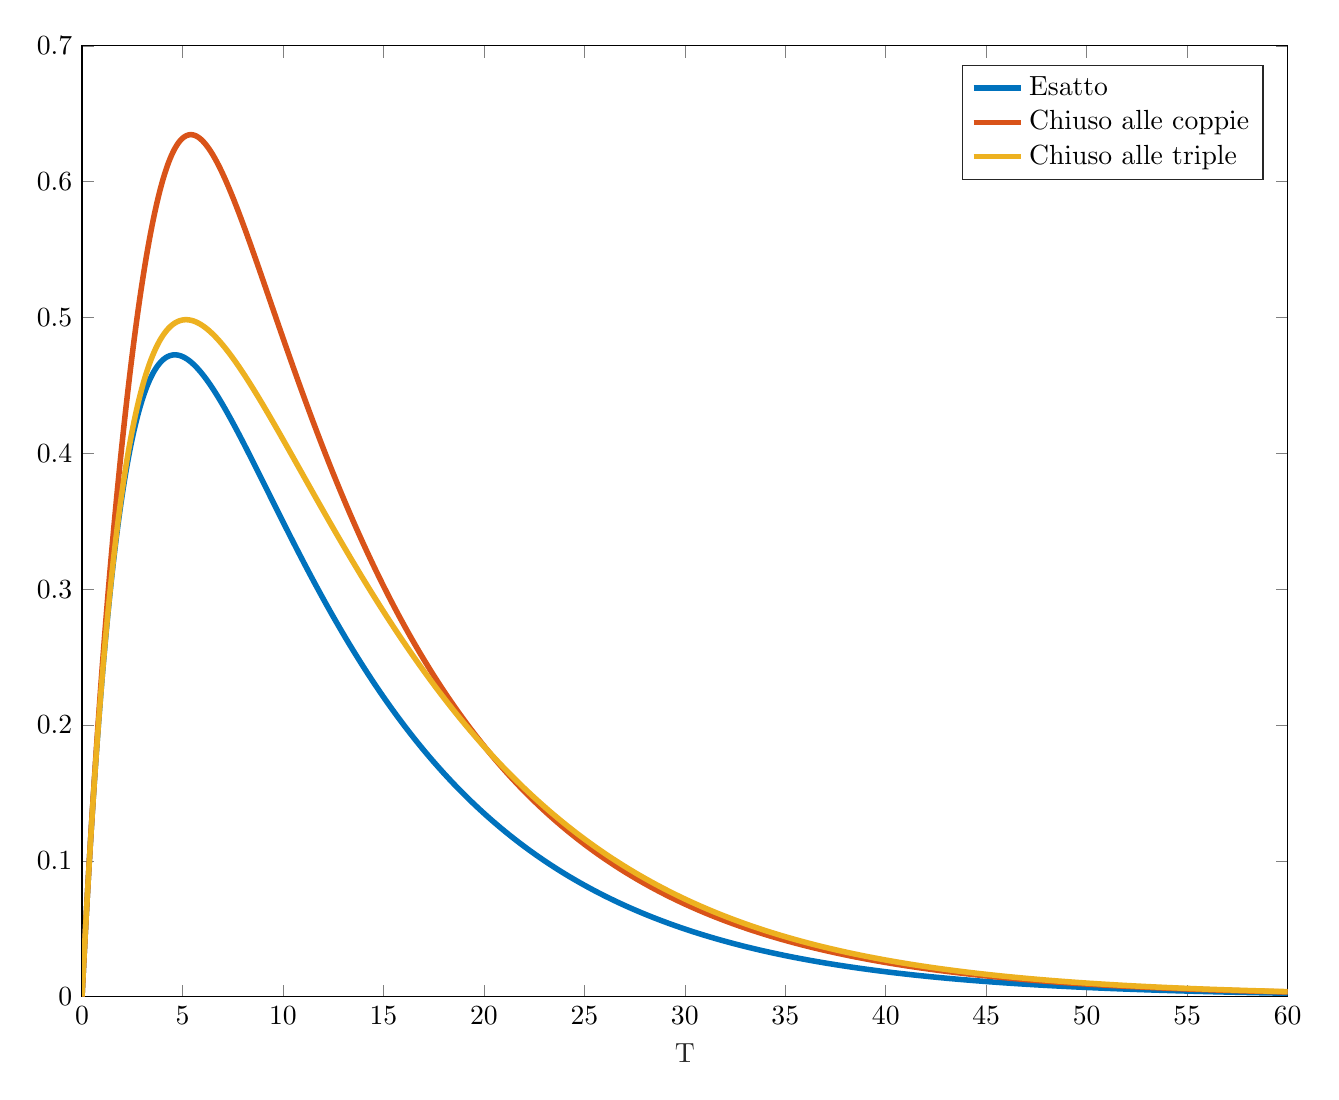
\begin{tikzpicture}

\begin{axis}[%
width=6.028in,
height=4.754in,
at={(1.011in,0.642in)},
scale only axis,
xmin=0,
xmax=60,
xlabel style={font=\color{white!15!black}},
xlabel={T},
ymin=0,
ymax=0.7,
axis background/.style={fill=white},
legend style={legend cell align=left, align=left, draw=white!15!black}
]
\addplot [color=mycolor1, line width=2.0pt]
  table[row sep=crcr]{%
0	0\\
0.00199053585276749	0.000596863671153253\\
0.00398107170553497	0.00119313350400473\\
0.00597160755830246	0.00178880999483315\\
0.00796214341106994	0.00238389363951781\\
0.0123567669950473	0.00369559815786577\\
0.0167513905790247	0.00500442076491133\\
0.0211460141630021	0.0063103667761891\\
0.0255406377469794	0.0076134414977999\\
0.0299388563931551	0.00891471270231856\\
0.0343370750393307	0.0102131185230324\\
0.0387352936855064	0.0115086642507384\\
0.043133512331682	0.0128013551668353\\
0.0475471725191068	0.014095719985606\\
0.0519608327065316	0.0153872205391668\\
0.0563744928939564	0.0166758621362425\\
0.0607881530813811	0.0179616500760944\\
0.0652173199794049	0.0192490920427435\\
0.0696464868774286	0.0205336709283775\\
0.0740756537754524	0.0218153920596138\\
0.0785048206734761	0.02309426075354\\
0.0829496187548012	0.0243747805506026\\
0.0873944168361263	0.0256524384408708\\
0.0918392149174515	0.0269272397690298\\
0.0962840129987766	0.0281991898701689\\
0.100744568101794	0.0294727880488508\\
0.105205123204811	0.0307435254851393\\
0.109665678307829	0.0320114075419652\\
0.114126233410846	0.0332764395725959\\
0.118602673075784	0.0345431166416037\\
0.123079112740721	0.035806934122553\\
0.127555552405659	0.0370678973968009\\
0.132031992070596	0.0383260118359723\\
0.136524445545197	0.0395857682528344\\
0.141016899019798	0.0408426662256896\\
0.1455093524944	0.042096711154504\\
0.150001805969001	0.043347908429443\\
0.154510404254387	0.044600744603141\\
0.159019002539772	0.0458507234663602\\
0.163527600825158	0.0470978504378629\\
0.168036199110544	0.0483421309265403\\
0.172561074936287	0.0495880472002203\\
0.17708595076203	0.0508311072862559\\
0.181610826587773	0.0520713166223946\\
0.186135702413515	0.0533086806364423\\
0.190676990405524	0.0545476773232978\\
0.195218278397533	0.0557838189343043\\
0.199759566389542	0.0570171109263876\\
0.204300854381551	0.05824755874646\\
0.208858690959197	0.0594796360902296\\
0.213416527536843	0.0607088594587309\\
0.217974364114488	0.0619352343282638\\
0.222532200692134	0.0631587661650419\\
0.227106724202768	0.0643839243658259\\
0.231681247713401	0.0656062296804019\\
0.236255771224035	0.0668256876046435\\
0.240830294734669	0.0680423036242643\\
0.245421645441331	0.0692605428236818\\
0.250012996147992	0.0704759302141823\\
0.254604346854654	0.0716884713114161\\
0.259195697561315	0.0728981716207982\\
0.263804017673384	0.0741094918988787\\
0.268412337785452	0.075317961433318\\
0.273020657897521	0.0765235857597491\\
0.27762897800959	0.0777263704034939\\
0.282254411746462	0.0789307717839793\\
0.286879845483334	0.0801323234738011\\
0.291505279220206	0.0813310310287846\\
0.296130712957079	0.0825268999943676\\
0.300773406613671	0.0837243824498247\\
0.305416100270264	0.084919016254977\\
0.310058793926856	0.0861108069860559\\
0.314701487583449	0.0872997602088277\\
0.319361589521735	0.0884903236462132\\
0.324021691460022	0.0896780394607686\\
0.328681793398309	0.0908629132493486\\
0.333341895336596	0.0920449505982641\\
0.338019556071109	0.09322859486866\\
0.342697216805623	0.0944093925304909\\
0.347374877540136	0.095587349201456\\
0.35205253827465	0.0967624704886312\\
0.356747910447269	0.0979391953683189\\
0.361443282619888	0.0991130746402484\\
0.366138654792507	0.100284113943189\\
0.370834026965126	0.101452318905204\\
0.375547265516765	0.102622124126224\\
0.380260504068404	0.103789084726424\\
0.384973742620042	0.104953206365872\\
0.389686981171681	0.106114494693849\\
0.394418243246227	0.107277379906657\\
0.399149505320772	0.108437421471469\\
0.403880767395317	0.109594625069886\\
0.408612029469863	0.110748996372638\\
0.41336147459102	0.111904961176813\\
0.418110919712177	0.113058083291295\\
0.422860364833334	0.114208368419451\\
0.427609809954491	0.115355822253699\\
0.432377599961091	0.116504866168302\\
0.437145389967691	0.117651068336707\\
0.44191317997429	0.118794434484295\\
0.44668096998089	0.119934970325409\\
0.451467269141767	0.121077092803393\\
0.456253568302644	0.122216374463503\\
0.461039867463521	0.123352821053378\\
0.465826166624398	0.124486438309531\\
0.47063114173014	0.125621638745407\\
0.475436116835881	0.126753999276135\\
0.480241091941623	0.127883525671864\\
0.485046067047365	0.129010223691529\\
0.489869887370685	0.130138501397382\\
0.494693707694006	0.131263940094895\\
0.499517528017326	0.132386545576981\\
0.504341348340647	0.133506323625253\\
0.509184185682064	0.134627677827418\\
0.51402702302348	0.135746193901808\\
0.518869860364897	0.136861877664363\\
0.523712697706314	0.137974734919629\\
0.528574726619363	0.139089164796174\\
0.533436755532412	0.140200757408737\\
0.53829878444546	0.141309518596548\\
0.543160813358509	0.142415454187355\\
0.548042211039569	0.143522958826793\\
0.55292360872063	0.144627627048926\\
0.55780500640169	0.145729464716545\\
0.56268640408275	0.146828477680867\\
0.56758735048985	0.14792905609415\\
0.572488296896949	0.149026798919262\\
0.577389243304049	0.150121712042838\\
0.582290189711149	0.151213801339834\\
0.587210867601438	0.152307452453023\\
0.592131545491728	0.153398268789234\\
0.597052223382018	0.154486256259217\\
0.601972901272307	0.155571420761955\\
0.606913496388328	0.156658143441472\\
0.611854091504349	0.157742032136696\\
0.61679468662037	0.158823092782783\\
0.621735281736391	0.159901331303027\\
0.626695982628195	0.160981124299581\\
0.631656683519999	0.162058084085729\\
0.636617384411802	0.163132216621328\\
0.641578085303606	0.164203527854271\\
0.646559083672327	0.165276389861819\\
0.651540082041047	0.166346419413431\\
0.656521080409768	0.167413622493963\\
0.661502078778488	0.168478005076203\\
0.666503569383853	0.169543934693833\\
0.671505059989219	0.170607032590131\\
0.676506550594584	0.171667304775254\\
0.68150804119995	0.172724757247195\\
0.686530221876942	0.173783752965696\\
0.691552402553934	0.174839917677204\\
0.696574583230927	0.17589325741749\\
0.701596763907919	0.176943778210055\\
0.706639835866396	0.17799583845766\\
0.711682907824873	0.179045068391679\\
0.71672597978335	0.180091474073811\\
0.721769051741827	0.181135061553381\\
0.72683321952555	0.182180184667736\\
0.731897387309272	0.183222478140426\\
0.736961555092995	0.184261948059406\\
0.742025722876718	0.185298600500149\\
0.747111194287107	0.186336784694121\\
0.752196665697496	0.187372139896476\\
0.757282137107885	0.188404672221754\\
0.762367608518274	0.189434387771903\\
0.767474594900923	0.190465631174043\\
0.772581581283573	0.191494046212103\\
0.777688567666222	0.192519639027544\\
0.782795554048871	0.193542415749128\\
0.78792427039055	0.194566716403007\\
0.793052986732229	0.195588189297166\\
0.798181703073909	0.196606840600332\\
0.803310419415588	0.19762267646842\\
0.808461084325784	0.19864003230843\\
0.81361174923598	0.199654560969335\\
0.818762414146177	0.200666268647482\\
0.823913079056373	0.201675161526289\\
0.82908591482452	0.20268557036897\\
0.834258750592667	0.20369315258887\\
0.839431586360813	0.204697914410312\\
0.84460442212896	0.205699862044578\\
0.849799655005291	0.20670332162286\\
0.854994887881621	0.207703955109619\\
0.860190120757951	0.208701768757523\\
0.865385353634282	0.209696768806081\\
0.870603213699137	0.210693276721919\\
0.875821073763992	0.21168695905188\\
0.881038933828848	0.212677822077353\\
0.886256793893703	0.213665872066451\\
0.891497515445601	0.214655425843533\\
0.896738236997499	0.215642154513897\\
0.901978958549397	0.216626064388038\\
0.907219680101295	0.217607161763051\\
0.912483501408722	0.218589758776462\\
0.917747322716149	0.21956953113531\\
0.923011144023576	0.220546485179584\\
0.928274965331004	0.221520627235754\\
0.933562128954513	0.222496264750526\\
0.938849292578023	0.223469078035106\\
0.944136456201532	0.224439073459383\\
0.949423619825042	0.225406257379597\\
0.954734372782572	0.226374932557155\\
0.960045125740102	0.227340783900258\\
0.965355878697632	0.228303817809101\\
0.970666631655162	0.229264040670107\\
0.976001225418392	0.23022575054283\\
0.981335819181621	0.231184636947445\\
0.98667041294485	0.232140706314877\\
0.99200500670808	0.233093965062146\\
0.997363697280812	0.23404870652321\\
1.00272238785355	0.23500062485239\\
1.00808107842628	0.235949726511769\\
1.01343976899901	0.236896017949392\\
1.0188228172289	0.237843787783297\\
1.02420586545878	0.238788734790457\\
1.02958891368867	0.23973086546455\\
1.03497196191855	0.240670186285087\\
1.04037963341625	0.241610981126741\\
1.04578730491395	0.242548953414934\\
1.05119497641164	0.24348410967539\\
1.05660264790934	0.24441645641953\\
1.06203521338424	0.245350272786539\\
1.06746777885913	0.246281266840504\\
1.07290034433402	0.247209445139657\\
1.07833290980891	0.248134814227787\\
1.08379064506731	0.24906164849204\\
1.08924838032571	0.249985660649904\\
1.09470611558411	0.250906857292591\\
1.10016385084252	0.251825244996726\\
1.1056470369148	0.252745093378341\\
1.11113022298707	0.253662119825547\\
1.11661340905935	0.254576330963018\\
1.12209659513163	0.255487733400699\\
1.12760551858231	0.256400591991415\\
1.13311444203298	0.257310628783914\\
1.13862336548365	0.258217850436829\\
1.14413228893432	0.259122263593915\\
1.14966724184116	0.260028128323363\\
1.15520219474799	0.260931171354033\\
1.16073714765482	0.261831399379022\\
1.16627210056166	0.262728819076401\\
1.17183338076584	0.263627685723182\\
1.17739466097002	0.264523730732774\\
1.18295594117419	0.265416960833255\\
1.18851722137837	0.266307382737531\\
1.19410513262804	0.267199246921074\\
1.19969304387772	0.268088289490049\\
1.20528095512739	0.268974517208057\\
1.21086886637706	0.269857936823364\\
1.21648371859449	0.270742794014333\\
1.22209857081192	0.27162482957315\\
1.22771342302936	0.272504050299476\\
1.23332827524679	0.273380462977487\\
1.23897038457538	0.274258308471657\\
1.24461249390397	0.275133332274722\\
1.25025460323256	0.276005541222972\\
1.25589671256115	0.276874942137045\\
1.26156640151281	0.277745771044898\\
1.26723609046446	0.278613778160169\\
1.27290577941612	0.279478970356349\\
1.27857546836778	0.280341354491114\\
1.28427306633634	0.281205161782002\\
1.28997066430491	0.282066147134783\\
1.29566826227347	0.282924317460739\\
1.30136586024204	0.283779679655171\\
1.30709170327692	0.284636460085816\\
1.31281754631181	0.285490418387634\\
1.31854338934669	0.286341561510305\\
1.32426923238158	0.287189896387357\\
1.33002366371043	0.288039644544449\\
1.33577809503928	0.288886570335292\\
1.34153252636813	0.289730680748588\\
1.34728695769699	0.290571982756714\\
1.35307032782915	0.291414693033373\\
1.35885369796131	0.292254580658218\\
1.36463706809348	0.293091652659611\\
1.37042043822564	0.293925916049414\\
1.37622881553645	0.294760966974212\\
1.38203719284726	0.295593199071865\\
1.38784557015807	0.296422619395436\\
1.39365394746888	0.29724923498135\\
1.39948194569202	0.298075831003058\\
1.40530994391516	0.29889961744773\\
1.41113794213829	0.29972060137296\\
1.41696594036143	0.300538789819638\\
1.4228137248248	0.30135695337945\\
1.42866150928816	0.302172316598042\\
1.43450929375153	0.302984886537666\\
1.44035707821489	0.3037946702438\\
1.44622478964653	0.304604419958342\\
1.45209250107816	0.305411378578768\\
1.45796021250979	0.306215553172018\\
1.46382792394143	0.307016950788192\\
1.46971570462452	0.307818305250468\\
1.4756034853076	0.308616877877142\\
1.48149126599069	0.309412675739878\\
1.48737904667378	0.310205705893425\\
1.49328704060906	0.31099868369102\\
1.49919503454433	0.311788888922936\\
1.50510302847961	0.312576328665591\\
1.51101102241489	0.313361009978419\\
1.51693937480906	0.314145629621035\\
1.52286772720322	0.314927485979802\\
1.52879607959739	0.315706586135926\\
1.53472443199155	0.316482937153554\\
1.540673290528	0.317259217238629\\
1.54662214906446	0.318032743332934\\
1.55257100760091	0.318803522522495\\
1.55851986613736	0.319571561876207\\
1.56448937947106	0.320339520884143\\
1.57045889280476	0.321104735206403\\
1.57642840613847	0.321867211933869\\
1.58239791947216	0.322626958140219\\
1.58838823791446	0.323386614523716\\
1.59437855635675	0.324143535538803\\
1.60036887479904	0.324897728281248\\
1.60635919324133	0.325649199829546\\
1.61237046959671	0.326400572114511\\
1.61838174595208	0.327149218359919\\
1.62439302230746	0.327895145666464\\
1.63040429866284	0.32863836111749\\
1.63643668672632	0.329381467707424\\
1.6424690747898	0.330121857599062\\
1.64850146285328	0.330859537898058\\
1.65453385091676	0.33159451569264\\
1.66058750665404	0.332329375014621\\
1.66664116239132	0.333061526991747\\
1.67269481812859	0.333790978734666\\
1.67874847386587	0.334517737336524\\
1.68482355500326	0.335244367784807\\
1.69089863614064	0.335968300254025\\
1.69697371727803	0.336689541859858\\
1.70304879841541	0.33740809970041\\
1.70914546464501	0.338126519657033\\
1.71524213087462	0.338842251012751\\
1.72133879710422	0.339555300888316\\
1.72743546333383	0.340265676386821\\
1.73355387572031	0.340975904147761\\
1.73967228810678	0.341683452698896\\
1.74579070049326	0.342388329166083\\
1.75190911287974	0.343090540657441\\
1.75804943463327	0.343792594521139\\
1.76418975638681	0.344491978578982\\
1.77033007814035	0.345188699961971\\
1.77647039989388	0.34588276578329\\
1.78263279664118	0.346576664074865\\
1.78879519338848	0.347267901977104\\
1.79495759013578	0.347956486626186\\
1.80111998688309	0.348642425140401\\
1.80730462566597	0.349328186092547\\
1.81348926444885	0.350011296085053\\
1.81967390323173	0.350691762259322\\
1.82585854201462	0.351369591738785\\
1.83206559217232	0.352047233588486\\
1.83827264233002	0.352722233921306\\
1.84447969248772	0.353394599883911\\
1.85068674264543	0.354064338604908\\
1.85691637550678	0.354733879553676\\
1.86314600836813	0.355400788441563\\
1.86937564122948	0.356065072420534\\
1.87560527409083	0.356726738624418\\
1.88185766319929	0.357388196858193\\
1.88811005230775	0.358047032500346\\
1.89436244141622	0.358703252708185\\
1.90061483052468	0.3593568646208\\
1.90689015093446	0.360010258231314\\
1.91316547134424	0.360661038733366\\
1.91944079175402	0.361309213289645\\
1.92571611216381	0.361954789044542\\
1.93201454150218	0.362600136138563\\
1.93831297084055	0.363242879620959\\
1.94461140017892	0.363883026659847\\
1.9509098295173	0.364520584404957\\
1.95723154808653	0.36515790310657\\
1.96355326665576	0.365792627706817\\
1.96987498522499	0.366424765379283\\
1.97619670379422	0.367054323279081\\
1.98254189319299	0.367683631584783\\
1.98888708259176	0.368310355313704\\
1.99523227199053	0.368934501644941\\
2.0015774613893	0.369556077739033\\
2.00794630624256	0.3701773936892\\
2.01431515109582	0.37079613460102\\
2.02068399594908	0.371412307659145\\
2.02705284080234	0.372025920029584\\
2.03344552746868	0.372639261573968\\
2.03983821413503	0.373250037632894\\
2.04623090080137	0.373858255396617\\
2.05262358746771	0.374463922036658\\
2.05904030495676	0.375069307120733\\
2.06545702244581	0.3756721362866\\
2.07187373993486	0.376272416730159\\
2.07829045742391	0.376870155628488\\
2.084731396657	0.377467602117917\\
2.0911723358901	0.378062502271274\\
2.0976132751232	0.378654863290148\\
2.1040542143563	0.379244692357219\\
2.11051956957009	0.379834218164606\\
2.11698492478388	0.380421207232392\\
2.12345027999767	0.381005666767906\\
2.12991563521146	0.381587603959477\\
2.13640560238783	0.382169226892256\\
2.1428955695642	0.382748322696976\\
2.14938553674057	0.383324898586751\\
2.15587550391694	0.383898961755605\\
2.16239028199053	0.38447269962306\\
2.16890506006412	0.385043919988883\\
2.17541983813771	0.385612630072026\\
2.1819346162113	0.386178837072254\\
2.18847440630977	0.386744707611715\\
2.19501419640825	0.387308070291313\\
2.20155398650673	0.387868932335878\\
2.20809377660521	0.38842730095097\\
2.21465878275268	0.388985321885443\\
2.22122378890015	0.389540844617099\\
2.22778879504762	0.390093876376703\\
2.23435380119508	0.390644424375653\\
2.24094422983074	0.391194613366607\\
2.24753465846639	0.391742313827424\\
2.25412508710205	0.392287532994854\\
2.2607155157377	0.392830278086184\\
2.2673315759421	0.393372652748923\\
2.27394763614649	0.393912548570056\\
2.28056369635089	0.394449972792368\\
2.28717975655528	0.394984932639088\\
2.29382166035897	0.395519510562987\\
2.30046356416266	0.396051619349689\\
2.30710546796636	0.396581266248067\\
2.31374737177005	0.39710845848734\\
2.32041533418655	0.397635257231925\\
2.32708329660306	0.398159596559648\\
2.33375125901957	0.398681483725524\\
2.34041922143607	0.399200925964814\\
2.34711345989709	0.399719963009676\\
2.3538076983581	0.400236550374444\\
2.36050193681912	0.400750695320328\\
2.36719617528013	0.401262405088688\\
2.37391691043736	0.401773697892413\\
2.3806376455946	0.402282550769205\\
2.38735838075183	0.402788970986522\\
2.39407911590907	0.403292965791876\\
2.40082657131283	0.403796531760668\\
2.40757402671659	0.404297667572316\\
2.41432148212035	0.404796380500586\\
2.42106893752412	0.405292677799196\\
2.42784333963791	0.405788534283187\\
2.4346177417517	0.406281970396727\\
2.4413921438655	0.406772993419943\\
2.44816654597929	0.407261610612817\\
2.4549681243632	0.407749774914683\\
2.4617697027471	0.408235528649874\\
2.46857128113101	0.408718879104942\\
2.47537285951492	0.409199833546183\\
2.48220184698832	0.40968032292709\\
2.48903083446173	0.4101584115623\\
2.49585982193513	0.410634106744844\\
2.50268880940853	0.411107415747396\\
2.50954544177924	0.411580247402125\\
2.51640207414995	0.412050688149689\\
2.52325870652066	0.412518745289656\\
2.53011533889137	0.412984426101138\\
2.53699985562036	0.413449617198909\\
2.54388437234935	0.413912427245533\\
2.55076888907833	0.414372863547183\\
2.55765340580732	0.414830933389462\\
2.5645660494942	0.415288501031752\\
2.57147869318108	0.41574369749675\\
2.57839133686796	0.41619653009729\\
2.58530398055484	0.416647006125536\\
2.59224499685821	0.417096967336677\\
2.59918601316159	0.417544567262657\\
2.60612702946496	0.417989813223041\\
2.61306804576833	0.418432712516606\\
2.62003768421203	0.418875084291462\\
2.62700732265572	0.419315104691512\\
2.63397696109942	0.419752781043108\\
2.64094659954311	0.420188120651714\\
2.64794511298781	0.420622919914516\\
2.65494362643251	0.421055377731441\\
2.6619421398772	0.421485501435701\\
2.6689406533219	0.421913298339501\\
2.67596829852112	0.422340541973112\\
2.68299594372033	0.422765454108388\\
2.69002358891955	0.423188042085462\\
2.69705123411877	0.423608313223354\\
2.70410827073433	0.424028018003143\\
2.71116530734989	0.424445401251489\\
2.71822234396545	0.424860470315518\\
2.72527938058101	0.425273232521124\\
2.73236607296869	0.425685415217706\\
2.73945276535637	0.426095286368701\\
2.74653945774405	0.426502853328296\\
2.75362615013173	0.426908123429332\\
2.76074276611797	0.427312800727092\\
2.76785938210422	0.427715176484567\\
2.77497599809046	0.428115258063073\\
2.78209261407671	0.428513052802469\\
2.78923942490227	0.428910241292782\\
2.79638623572783	0.429305138268119\\
2.80353304655339	0.429697751096998\\
2.81067985737896	0.430088087126362\\
2.81785713902212	0.430477803376319\\
2.82503442066529	0.430865238156383\\
2.83221170230846	0.431250398842348\\
2.83938898395163	0.431633292788315\\
2.84659701614953	0.43201555327806\\
2.85380504834743	0.43239554236323\\
2.86101308054533	0.43277326742697\\
2.86822111274323	0.433148735830612\\
2.87546017926332	0.433523556963159\\
2.88269924578341	0.433896116777026\\
2.88993831230351	0.434266422662785\\
2.8971773788236	0.434634481989074\\
2.90444776780364	0.435001880101966\\
2.91171815678368	0.435367027002837\\
2.91898854576373	0.435729930089766\\
2.92625893474377	0.436090596738771\\
2.93356093845992	0.436450588085573\\
2.94086294217606	0.436808338348176\\
2.94816494589221	0.437163854932239\\
2.95546694960836	0.437517145221242\\
2.96280086487659	0.437869745985594\\
2.97013478014483	0.438220115814937\\
2.97746869541306	0.438568262122592\\
2.9848026106813	0.438914192299578\\
2.99216873909201	0.439259418598997\\
2.99953486750271	0.439602424134099\\
3.00690099591342	0.439943216325953\\
3.01426712432413	0.440281802573197\\
3.02166577186631	0.440619670433932\\
3.02906441940849	0.440955327722978\\
3.03646306695067	0.441288781869232\\
3.04386171449286	0.441620040279033\\
3.05129319192691	0.441950565647343\\
3.05872466936097	0.442278890658793\\
3.06615614679503	0.442605022750196\\
3.07358762422909	0.442928969335675\\
3.08105224696524	0.443252168065618\\
3.0885168697014	0.443573176676142\\
3.09598149243755	0.443892002612064\\
3.1034461151737	0.444208653295379\\
3.11094420406679	0.44452454117647\\
3.11844229295988	0.444838249198212\\
3.12594038185297	0.445149784813515\\
3.13343847074605	0.445459155452332\\
3.14097035080817	0.445767748147201\\
3.14850223087028	0.446074171266256\\
3.1560341109324	0.446378432270588\\
3.16356599099451	0.446680538598196\\
3.17113199342146	0.446981851721224\\
3.17869799584842	0.447281005575169\\
3.18626399827537	0.447578007629397\\
3.19383000070233	0.44787286533005\\
3.20143046110215	0.448166914366232\\
3.20903092150198	0.448458814464092\\
3.21663138190181	0.448748573101365\\
3.22423184230164	0.449036197732424\\
3.2318671021242	0.449322998088722\\
3.23950236194676	0.449607659861573\\
3.24713762176933	0.449890190537181\\
3.25477288159189	0.450170597578242\\
3.26244328804483	0.450450164570876\\
3.27011369449776	0.450727603359274\\
3.2777841009507	0.451002921438206\\
3.28545450740363	0.451276126278793\\
3.29316041266953	0.451548475097165\\
3.30086631793543	0.451818706115582\\
3.30857222320133	0.45208682683748\\
3.31627812846722	0.452352844742503\\
3.32401989110489	0.452617990493408\\
3.33176165374256	0.452881028873745\\
3.33950341638023	0.453141967395721\\
3.3472451790179	0.453400813547605\\
3.35502316313618	0.453658771217297\\
3.36280114725446	0.453914631971493\\
3.37057913137275	0.454168403331276\\
3.37835711549103	0.454420092793642\\
3.38617169154667	0.454670877267849\\
3.3939862676023	0.454919575307546\\
3.40180084365794	0.455166194442796\\
3.40961541971357	0.455410742179432\\
3.41746696420648	0.455654368224826\\
3.42531850869938	0.455895918343089\\
3.43317005319229	0.456135400073376\\
3.4410215976852	0.456372820930461\\
3.44891049346576	0.456609303197031\\
3.45679938924632	0.456843720070645\\
3.46468828502688	0.457076079099665\\
3.47257718080744	0.457306387807917\\
3.48050381756295	0.457535740835241\\
3.48843045431847	0.457763039030825\\
3.49635709107398	0.457988289952354\\
3.50428372782949	0.458211501132818\\
3.51224850159594	0.458433739326967\\
3.52021327536239	0.458653933278224\\
3.52817804912884	0.458872090553714\\
3.53614282289529	0.459088218695711\\
3.54414613607264	0.459303356323371\\
3.55214944924998	0.459516460325292\\
3.56015276242733	0.459727538278159\\
3.56815607560468	0.459936597733642\\
3.57619833889781	0.460144648966411\\
3.58424060219095	0.460350677218681\\
3.59228286548408	0.460554690076818\\
3.60032512877721	0.460756695102015\\
3.60840675922679	0.460957673952982\\
3.61648838967638	0.461156640497664\\
3.62457002012596	0.461353602332236\\
3.63265165057554	0.461548567027538\\
3.64077307248204	0.461742487369245\\
3.64889449438855	0.461934406108372\\
3.65701591629505	0.462124330851033\\
3.66513733820155	0.462312269177839\\
3.67329898353354	0.462499144743726\\
3.68146062886554	0.462684029440648\\
3.68962227419754	0.46286693088479\\
3.69778391952953	0.463047856666663\\
3.70598622860803	0.463227701056948\\
3.71418853768653	0.463405565341989\\
3.72239084676502	0.463581457148181\\
3.73059315584352	0.46375538407607\\
3.73883657626523	0.463928210723821\\
3.74707999668693	0.464099068060992\\
3.75532341710863	0.464267963724323\\
3.76356683753034	0.464434905324533\\
3.77185182516863	0.464600727510149\\
3.78013681280692	0.464764591211249\\
3.78842180044522	0.464926504075057\\
3.79670678808351	0.465086473722605\\
3.80503380745825	0.465245304571455\\
3.81336082683299	0.46540218779365\\
3.82168784620774	0.465557131047051\\
3.83001486558248	0.465710141963141\\
3.83838438958511	0.46586199443042\\
3.84675391358775	0.466011910161359\\
3.85512343759039	0.4661598968246\\
3.86349296159302	0.46630596206223\\
3.8719054722877	0.466450848938694\\
3.88031798298237	0.466593810001986\\
3.88873049367705	0.466734852931685\\
3.89714300437172	0.46687398538063\\
3.90559899284027	0.46701191927937\\
3.91405498130882	0.467147938321561\\
3.92251096977737	0.467282050197877\\
3.93096695824593	0.467414262572063\\
3.93946692479213	0.467545255922613\\
3.94796689133833	0.46767434540733\\
3.95646685788454	0.467801538728144\\
3.96496682443074	0.467926843559866\\
3.97351127881372	0.468050908602618\\
3.98205573319669	0.468173080805007\\
3.99060018757967	0.468293367880385\\
3.99914464196265	0.46841177751479\\
4.00773410425464	0.468528926303614\\
4.01632356654662	0.468644193312717\\
4.02491302883861	0.468757586267042\\
4.0335024911306	0.468869112864024\\
4.04213749081375	0.46897935724313\\
4.05077249049689	0.469087730939286\\
4.05940749018004	0.469194241689198\\
4.06804248986318	0.469298897201865\\
4.07672356764034	0.469402248820481\\
4.08540464541749	0.469503740889349\\
4.09408572319465	0.469603381157121\\
4.10276680097181	0.469701177344537\\
4.11149450824228	0.469797647637758\\
4.12022221551276	0.469892269551559\\
4.12894992278323	0.469985050846721\\
4.1376776300537	0.470075999255907\\
4.14645252883691	0.470165599433958\\
4.15522742762012	0.470253362440913\\
4.16400232640333	0.470339296049872\\
4.17277722518654	0.470423408005607\\
4.18159988926615	0.470506149055944\\
4.19042255334575	0.470587064182053\\
4.19924521742536	0.470666161169543\\
4.20806788150496	0.470743447775488\\
4.21693889629988	0.470819340449629\\
4.22580991109479	0.470893418485711\\
4.23468092588971	0.470965689682059\\
4.24355194068463	0.471036161808242\\
4.2524719033702	0.471105216612397\\
4.26139186605577	0.471172468104846\\
4.27031182874135	0.47123792409683\\
4.27923179142692	0.471301592370618\\
4.28820131218307	0.471363819564693\\
4.29717083293922	0.471424254814136\\
4.30614035369538	0.471482905943317\\
4.31510987445153	0.47153978074741\\
4.32412957614907	0.471595190329869\\
4.33314927784661	0.47164881937634\\
4.34216897954416	0.47170067572454\\
4.3511886812417	0.471750767182765\\
4.36025919971018	0.471799368881431\\
4.36932971817866	0.471846201495246\\
4.37840023664715	0.471891272875497\\
4.38747075511563	0.471934590843818\\
4.39659274002011	0.471976394109516\\
4.40571472492458	0.472016439784751\\
4.41483670982906	0.472054735734612\\
4.42395869473353	0.4720912897943\\
4.43313280988389	0.472126303789722\\
4.44230692503424	0.472159571733162\\
4.45148104018459	0.47219110150375\\
4.46065515533495	0.472220900950482\\
4.469882079136	0.472249134539556\\
4.47910900293706	0.47227563366009\\
4.48833592673811	0.472300406205495\\
4.49756285053916	0.47232346003881\\
4.50684327607396	0.472344921774739\\
4.51612370160877	0.472364660671568\\
4.52540412714357	0.472382684637244\\
4.53468455267837	0.472399001549094\\
4.54401918924822	0.472413699665735\\
4.55335382581807	0.472426686619395\\
4.56268846238792	0.47243797033282\\
4.57202309895777	0.472447558697878\\
4.58141267108196	0.472455501094029\\
4.59080224320616	0.472461744051271\\
4.60019181533036	0.472466295507411\\
4.60958138745456	0.472469163369126\\
4.61902663678989	0.472470357598969\\
4.62847188612523	0.472469864162718\\
4.63791713546056	0.472467691013523\\
4.6473623847959	0.472463846073138\\
4.65686406984621	0.472458299331588\\
4.66636575489653	0.472451076746644\\
4.67586743994685	0.472442186287081\\
4.68536912499717	0.472431635890014\\
4.69492802222378	0.472419354999194\\
4.7044869194504	0.472405410138549\\
4.71404581667701	0.472389809292776\\
4.72360471390363	0.47237256041464\\
4.73320764525141	0.472353580627895\\
4.74281057659919	0.472332953582446\\
4.75241350794698	0.472310687244462\\
4.76201643929476	0.47228678954809\\
4.77165794452804	0.472261162616792\\
4.78129944976131	0.472233907125805\\
4.79094095499459	0.472205031008188\\
4.80058246022786	0.472174542164962\\
4.81026314694842	0.472142314778131\\
4.81994383366897	0.472108477397234\\
4.82962452038952	0.472073037922871\\
4.83930520711008	0.472036004223585\\
4.84902565638322	0.471997222246744\\
4.85874610565637	0.471956848723733\\
4.86846655492951	0.471914891523243\\
4.87818700420266	0.471871358481893\\
4.88794780523678	0.471826066922258\\
4.89770860627089	0.471779202150329\\
4.90746940730501	0.471730772003437\\
4.91723020833913	0.47168078428681\\
4.92703195872998	0.471629027305312\\
4.93683370912084	0.471575715335039\\
4.9466354595117	0.471520856182496\\
4.95643720990256	0.471464457622058\\
4.96628051524823	0.471406278548661\\
4.97612382059389	0.471346562603474\\
4.98596712593956	0.471285317562697\\
4.99581043128522	0.471222551170372\\
5.00569590732134	0.471157992504663\\
5.01558138335745	0.471091914980799\\
5.02546685939356	0.471024326345195\\
5.03535233542967	0.470955234312072\\
5.04528060635073	0.47088433774398\\
5.05520887727179	0.470811940231785\\
5.06513714819285	0.470738049492622\\
5.07506541911391	0.470662673211393\\
5.08503711889176	0.470585479625237\\
5.0950088186696	0.470506802912845\\
5.10498051844744	0.470426650762573\\
5.11495221822528	0.470345030830502\\
5.12496799094167	0.47026158031311\\
5.13498376365806	0.470176664394529\\
5.14499953637444	0.470090290734826\\
5.15501530909083	0.470002466961747\\
5.16507580953502	0.469912798807676\\
5.17513630997921	0.469821682887892\\
5.18519681042339	0.469729126834659\\
5.19525731086758	0.469635138247869\\
5.2053632039849	0.46953929097422\\
5.21546909710223	0.469442013484242\\
5.22557499021955	0.469343313382869\\
5.23568088333688	0.469243198242615\\
5.24583284576096	0.469141209585357\\
5.25598480818505	0.469037808178166\\
5.26613677060914	0.468933001599124\\
5.27628873303322	0.468826797393828\\
5.28648745229033	0.468718704324519\\
5.29668617154743	0.468609215892103\\
5.30688489080453	0.468498339648266\\
5.31708361006163	0.468386083112153\\
5.32732978639303	0.468271921828741\\
5.33757596272443	0.468156382492463\\
5.34782213905582	0.468039472629068\\
5.35806831538722	0.467921199731699\\
5.36836266133408	0.467801005670475\\
5.37865700728095	0.467679450793237\\
5.38895135322782	0.467556542600251\\
5.39924569917468	0.467432288559108\\
5.40958894010065	0.46730609639739\\
5.41993218102661	0.467178560586275\\
5.43027542195257	0.467049688600992\\
5.44061866287853	0.466919487884024\\
5.45101153706255	0.466787331547587\\
5.46140441124658	0.466653848661358\\
5.4717972854306	0.466519046675967\\
5.48219015961463	0.466382933009228\\
5.49263341945276	0.466244845665623\\
5.50307667929089	0.466105448807833\\
5.51351993912902	0.465964749862328\\
5.52396319896715	0.465822756222682\\
5.53445761187213	0.465678770276038\\
5.54495202477712	0.465533491789728\\
5.5554464376821	0.465386928166495\\
5.56594085058709	0.465239086776103\\
5.57648719831941	0.465089233882723\\
5.58703354605173	0.464938105366306\\
5.59757989378405	0.464785708606295\\
5.60812624151637	0.464632050949068\\
5.61872532103302	0.464476362013688\\
5.62932440054967	0.464319414317114\\
5.63992348006633	0.464161215215917\\
5.65052255958298	0.464001772033507\\
5.66117518401188	0.463840277202269\\
5.67182780844078	0.463677540419899\\
5.68248043286967	0.463513569020514\\
5.69313305729857	0.463348370304978\\
5.70384005671797	0.463181098959867\\
5.71454705613736	0.463012602424867\\
5.72525405555675	0.46284288801206\\
5.73596105497615	0.462671963000176\\
5.74672327665992	0.462498943761168\\
5.75748549834369	0.462324716047747\\
5.76824772002746	0.462149287150375\\
5.77900994171123	0.461972664326062\\
5.78982825023888	0.461793925056129\\
5.80064655876654	0.461613993984669\\
5.81146486729419	0.461432878380938\\
5.82228317582184	0.46125058548063\\
5.83315845473553	0.461066153265422\\
5.84403373364921	0.460880545881946\\
5.8549090125629	0.460693770578662\\
5.86578429147658	0.460505834570355\\
5.87671744355088	0.460315735719093\\
5.88765059562518	0.460124478296268\\
5.89858374769948	0.459932069529954\\
5.90951689977378	0.459738516614436\\
5.92050884813521	0.459542776646387\\
5.93150079649664	0.459345894669942\\
5.94249274485807	0.459147877893197\\
5.9534846932195	0.458948733490337\\
5.96453638108293	0.458747377145254\\
5.97558806894636	0.458544895324652\\
5.98663975680979	0.458341295217055\\
5.99769144467322	0.458136583976952\\
6.00880383710542	0.457929635189838\\
6.01991622953761	0.457721577432864\\
6.0310286219698	0.457512417875391\\
6.042141014402	0.457302163652609\\
6.05331509935885	0.457089645539645\\
6.0644891843157	0.456876034938335\\
6.07566326927256	0.456661338999279\\
6.08683735422941	0.456445564838774\\
6.09807414230094	0.456227499707649\\
6.10931093037248	0.456008358548873\\
6.12054771844401	0.455788148494695\\
6.13178450651555	0.455566876642917\\
6.14308503319571	0.455343285955411\\
6.15438555987588	0.455118635683239\\
6.16568608655605	0.454892932940705\\
6.17698661323621	0.45466618480752\\
6.18835193888863	0.454437089185282\\
6.19971726454106	0.454206950407001\\
6.21108259019348	0.453975775569443\\
6.2224479158459	0.453743571734629\\
6.23387912710053	0.453508990937518\\
6.24531033835517	0.453273383401949\\
6.2567415496098	0.453036756207555\\
6.26817276086443	0.452799116399073\\
6.2796709718506	0.452559069305827\\
6.29116918283678	0.452318011884016\\
6.30266739382295	0.452075951196557\\
6.31416560480912	0.451832894271304\\
6.32573195844141	0.451587398858505\\
6.33729831207371	0.451340909522736\\
6.34886466570601	0.451093433310609\\
6.36043101933831	0.450844977233503\\
6.37206668825559	0.450594050561532\\
6.38370235717287	0.450342146371388\\
6.39533802609016	0.450089271693795\\
6.40697369500744	0.449835433524068\\
6.41867988207414	0.449579091732986\\
6.43038606914084	0.449321788831432\\
6.44209225620754	0.449063531834658\\
6.45379844327423	0.448804327722331\\
6.46557638449348	0.448542585975358\\
6.47735432571273	0.448279899532032\\
6.48913226693197	0.448016275392558\\
6.50091020815122	0.447751720521367\\
6.51276117329228	0.44748459299672\\
6.52461213843333	0.447216537199994\\
6.53646310357439	0.446947560116773\\
6.54831406871544	0.446677668696676\\
6.56023936237899	0.446405168570769\\
6.57216465604253	0.446131756611109\\
6.58408994970607	0.445857439789091\\
6.59601524336962	0.445582225039945\\
6.608016207688	0.445304364433333\\
6.62001717200638	0.445025608449168\\
6.63201813632476	0.444745964045094\\
6.64401910064313	0.444465438142385\\
6.65609711612489	0.444182228107154\\
6.66817513160664	0.443898139172511\\
6.68025314708839	0.443613178282795\\
6.69233116257014	0.443327352345758\\
6.70448764976455	0.443038802834864\\
6.71664413695897	0.442749390928838\\
6.72880062415338	0.442459123559166\\
6.7409571113478	0.442168007620522\\
6.75319353351478	0.441874127433075\\
6.76542995568177	0.441579401385133\\
6.77766637784875	0.441283836395787\\
6.78990280001574	0.440987439347083\\
6.80222066442117	0.440688236105756\\
6.8145385288266	0.440388203573388\\
6.82685639323203	0.440087348657137\\
6.83917425763746	0.439785678226884\\
6.85157511856051	0.439481158314443\\
6.86397597948357	0.439175825719718\\
6.87637684040662	0.438869687338417\\
6.88877770132968	0.438562750028721\\
6.90126316148383	0.438252918562661\\
6.91374862163799	0.437942291067157\\
6.92623408179214	0.437630874426949\\
6.93871954194629	0.437318675488998\\
6.95129125486549	0.437003536273437\\
6.96386296778468	0.436687617730301\\
6.97643468070388	0.436370926733864\\
6.98900639362307	0.43605347012035\\
7.00166606764739	0.435733025557584\\
7.0143257416717	0.435411818423114\\
7.02698541569601	0.435089855581253\\
7.03964508972033	0.434767143857997\\
7.05239448925109	0.434441394928118\\
7.06514388878186	0.434114900241773\\
7.07789328831262	0.433787666653842\\
7.09064268784339	0.433459700980599\\
7.10348363709426	0.433128647159184\\
7.11632458634514	0.432796864461405\\
7.12916553559601	0.432464359733244\\
7.14200648484689	0.432131139781787\\
7.15494087138423	0.431794778962328\\
7.16787525792157	0.431457706217174\\
7.18080964445891	0.431119928383964\\
7.19374403099625	0.430781452261134\\
7.20677380774895	0.430439780717652\\
7.21980358450165	0.430097414275829\\
7.23283336125435	0.429754359765531\\
7.24586313800706	0.429410623977108\\
7.25899032889946	0.429063636233242\\
7.27211751979186	0.428715970701264\\
7.28524471068426	0.428367634203862\\
7.29837190157667	0.428018633523874\\
7.31159860422458	0.427666322298429\\
7.32482530687249	0.427313350484619\\
7.3380520095204	0.42695972489856\\
7.35127871216831	0.426605452316178\\
7.36460710304072	0.426247808404767\\
7.37793549391314	0.425889521201135\\
7.39126388478556	0.425530597515459\\
7.40459227565797	0.425171044117377\\
7.41802461355885	0.424808056319301\\
7.43145695145972	0.424444442628904\\
7.4448892893606	0.424080209851084\\
7.45832162726148	0.423715364749832\\
7.47186025959003	0.423347019721585\\
7.48539889191859	0.422978066312305\\
7.49893752424715	0.422608511322295\\
7.51247615657571	0.422238361510567\\
7.52612352432791	0.421864643653573\\
7.53977089208011	0.421490335046327\\
7.55341825983232	0.421115442485251\\
7.56706562758452	0.42073997272508\\
7.58082427117841	0.420360864052495\\
7.5945829147723	0.419981182388515\\
7.60834155836619	0.419600934526427\\
7.62210020196009	0.419220127217415\\
7.63597276754062	0.418835607209201\\
7.64984533312116	0.418450532105625\\
7.66371789870169	0.418064908697618\\
7.67759046428223	0.417678743733579\\
7.69157971106386	0.417288789164432\\
7.70556895784549	0.416898297542767\\
7.71955820462712	0.416507275657974\\
7.73354745140875	0.416115730256467\\
7.7476562591015	0.415720315023038\\
7.76176506679424	0.415324380937006\\
7.77587387448699	0.414927934787085\\
7.78998268217974	0.41453098331854\\
7.80421406003167	0.414130078223526\\
7.81844543788359	0.41372867264379\\
7.83267681573552	0.413326773368272\\
7.84690819358745	0.412924387141975\\
7.86126528820976	0.412517959714703\\
7.87562238283208	0.412111050350282\\
7.8899794774544	0.411703665838832\\
7.90433657207672	0.411295812926031\\
7.91882267896367	0.410883827141941\\
7.93330878585062	0.410471378160413\\
7.94779489273757	0.41005847277376\\
7.96228099962452	0.409645117729317\\
7.97689957365268	0.409227533760842\\
7.99151814768085	0.408809505540174\\
8.00613672170902	0.408391039862889\\
8.02075529573718	0.407972143479027\\
8.03550996276884	0.407548917419143\\
8.0502646298005	0.407125266272281\\
8.06501929683216	0.406701196838414\\
8.07977396386382	0.406276715871399\\
8.09466853533245	0.405847799376139\\
8.10956310680107	0.405418477194569\\
8.12445767826969	0.404988756132272\\
8.13935224973832	0.404558642948105\\
8.15439073744049	0.40412398287751\\
8.16942922514267	0.403688936773471\\
8.18446771284484	0.403253511448477\\
8.19950620054702	0.402817713667644\\
8.2146928332504	0.402377251680097\\
8.22987946595378	0.401936423582314\\
8.24506609865717	0.401495236195066\\
8.26025273136055	0.401053696291085\\
8.27559197362809	0.400607368380022\\
8.29093121589562	0.400160694571953\\
8.30627045816316	0.399713681697421\\
8.32160970043069	0.399266336538218\\
8.33710627308224	0.398814072528804\\
8.35260284573378	0.398361483147093\\
8.36809941838533	0.397908575234993\\
8.38359599103687	0.39745535558492\\
8.39925489573158	0.396997078519423\\
8.41491380042629	0.396538496941191\\
8.430572705121	0.396079617705224\\
8.44623160981571	0.395620447616237\\
8.46205815432056	0.395156073129313\\
8.4778846988254	0.394691415349728\\
8.49371124333024	0.394226481147433\\
8.50953778783509	0.393761277341269\\
8.52553761739547	0.393290712868596\\
8.54153744695585	0.392819886711985\\
8.55753727651623	0.39234880575836\\
8.57353710607661	0.39187747684266\\
8.58971623619016	0.391400620802009\\
8.60589536630372	0.390923525105863\\
8.62207449641727	0.390446196660322\\
8.63825362653082	0.389968642318571\\
8.65461848330403	0.38948538308424\\
8.67098334007723	0.389001906676914\\
8.68734819685043	0.388518220024275\\
8.70371305362364	0.388034330000101\\
8.72018188980809	0.387547167009767\\
8.73665072599255	0.387059811857677\\
8.75311956217701	0.386572271385131\\
8.76958839836146	0.386084552379636\\
8.78614348346302	0.385594106002318\\
8.80269856856458	0.385103492806849\\
8.81925365366614	0.384612719524581\\
8.83580873876771	0.384121792833435\\
8.85245111606455	0.383628129632274\\
8.86909349336139	0.38313432477008\\
8.88573587065824	0.382640384868686\\
8.90237824795508	0.382146316496854\\
8.91910883699713	0.381649506436019\\
8.93583942603918	0.38115257968993\\
8.95257001508123	0.380655542771152\\
8.96930060412328	0.380158402139538\\
8.98612034063892	0.379658514464395\\
9.00294007715455	0.379158534900188\\
9.01975981367019	0.37865846985046\\
9.03657955018582	0.378158325666403\\
9.05348938408815	0.377655428976182\\
9.07039921799048	0.377152465015296\\
9.08730905189281	0.376649440078508\\
9.10421888579513	0.37614636040859\\
9.12121978296026	0.375640522617389\\
9.13822068012539	0.375134641997925\\
9.15522157729052	0.374628724736418\\
9.17222247445565	0.374122776967458\\
9.18931541587169	0.373614065343639\\
9.20640835728774	0.37310533515978\\
9.22350129870378	0.372596592493788\\
9.24059424011982	0.372087843372304\\
9.25778022278737	0.371576324526102\\
9.27496620545493	0.371064811215728\\
9.29215218812249	0.370553309411004\\
9.30933817079004	0.370041825030844\\
9.32661820779546	0.369527564926854\\
9.34389824480088	0.369013334284044\\
9.3611782818063	0.368499138964367\\
9.37845831881172	0.367984984779236\\
9.39583344002363	0.367468048730639\\
9.41320856123555	0.366951165899908\\
9.43058368244747	0.366434342041342\\
9.44795880365938	0.365917582859065\\
9.46543005570071	0.365398035543721\\
9.48290130774205	0.364878565036124\\
9.50037255978338	0.364359176983127\\
9.51784381182471	0.363839876981776\\
9.53541225878365	0.36331778243663\\
9.55298070574258	0.362795788124186\\
9.57054915270152	0.362273899584052\\
9.58811759966045	0.361752122306399\\
9.60578432346384	0.361227543932268\\
9.62345104726722	0.360703089052758\\
9.64111777107061	0.360178763100432\\
9.658784494874	0.35965457145878\\
9.67655059520445	0.35912757203901\\
9.6943166955349	0.358600719214647\\
9.71208279586536	0.358074018311396\\
9.72984889619581	0.357547474606257\\
9.74771549159443	0.357018116290506\\
9.76558208699305	0.356488927511739\\
9.78344868239167	0.355959913488983\\
9.80131527779029	0.355431079392935\\
9.81928350543996	0.354899423720483\\
9.83725173308963	0.354367960369309\\
9.8552199607393	0.353836694451941\\
9.87318818838897	0.35330563103295\\
9.89125920482513	0.352771738928825\\
9.90933022126129	0.352238061774941\\
9.92740123769745	0.351704604577494\\
9.94547225413361	0.351171372295099\\
9.96364723590061	0.350635304068253\\
9.9818222176676	0.350099473267245\\
9.99999719943459	0.349563884792105\\
10.0181721812016	0.349028543495651\\
10.0364523247657	0.348490358859464\\
10.0547324683298	0.347952433973322\\
10.0730126118939	0.347414773631238\\
10.0912927554579	0.346877382580397\\
10.1096792783833	0.346337140636305\\
10.1280658013086	0.34579718061708\\
10.146452324234	0.345257507210869\\
10.1648388471593	0.344718125059366\\
10.1833329877765	0.344175884325335\\
10.2018271283938	0.343633947543609\\
10.220321269011	0.343092319296608\\
10.2388154096282	0.342551004120678\\
10.257418428294	0.342006822513267\\
10.2760214469598	0.341462966740257\\
10.2946244656257	0.340919441278473\\
10.3132274842915	0.340376250559044\\
10.3319406634311	0.339830185411715\\
10.3506538425707	0.339284467837587\\
10.3693670217104	0.33873910220801\\
10.38808020085	0.338194092849027\\
10.4069048454226	0.33764620091841\\
10.4257294899953	0.337098678158556\\
10.4445541345679	0.336551528835458\\
10.4633787791406	0.336004757170186\\
10.4823162175897	0.335455094628707\\
10.5012536560388	0.334905822716411\\
10.5201910944879	0.33435694559404\\
10.539128532937	0.333808467377797\\
10.5581801172831	0.333257089831792\\
10.5772317016292	0.332706124236341\\
10.5962832859753	0.332155574647034\\
10.6153348703214	0.331605445075309\\
10.6345019773376	0.331052407552174\\
10.6536690843538	0.330499803166059\\
10.67283619137	0.329947635867491\\
10.6920032983861	0.32939590956323\\
10.7112873293394	0.328841266540646\\
10.7305713602926	0.328287077708767\\
10.7498553912458	0.327733346913133\\
10.769139422199	0.327180077955911\\
10.7885418041401	0.326623883346748\\
10.8079441860811	0.326068163851367\\
10.8273465680222	0.325512923210395\\
10.8467489499633	0.324958165121474\\
10.8662711360792	0.324400472286402\\
10.8857933221952	0.323843275359772\\
10.9053155083112	0.32328657797735\\
10.9248376944271	0.322730383732318\\
10.9444811647161	0.322171245483657\\
10.9641246350051	0.32161262381188\\
10.9837681052941	0.321054522247951\\
11.0034115755831	0.320496944280637\\
11.02317783773	0.319936412881104\\
11.0429440998769	0.319376418602928\\
11.0627103620238	0.318816964872306\\
11.0824766241707	0.318258055073637\\
11.102367213876	0.317696182251282\\
11.1222578035813	0.317134866973036\\
11.1421483932866	0.316574112560355\\
11.1620389829919	0.316013922293299\\
11.182055464688	0.315450759245942\\
11.202071946384	0.314888174045994\\
11.22208842808	0.314326169910187\\
11.2421049097761	0.313764750014263\\
11.2622488777205	0.313200347403998\\
11.282392845665	0.312636542827307\\
11.3025368136094	0.312073339396206\\
11.3226807815539	0.311510740182124\\
11.3429428732039	0.310945454506425\\
11.363204964854	0.310380786264233\\
11.3834670565041	0.309816738457989\\
11.4037291481542	0.309253314050037\\
11.4240073959591	0.308690067461389\\
11.444285643764	0.308127451081506\\
11.464563891569	0.307565467760121\\
11.4848421393739	0.307004120308155\\
11.5051410232308	0.306442841221611\\
11.5254399070878	0.305882204818697\\
11.5457387909448	0.305322213802973\\
11.5660376748017	0.304762870840404\\
11.5863613245615	0.304203497318489\\
11.6066849743212	0.303644778667038\\
11.627008624081	0.303086717449386\\
11.6473322738407	0.302529316192428\\
11.6676846007299	0.301971792284792\\
11.6880369276191	0.301414935163456\\
11.7083892545083	0.300858747257004\\
11.7287415813975	0.300303230958677\\
11.7491263024508	0.29974750603962\\
11.7695110235041	0.299192459567357\\
11.7898957445574	0.298638093840767\\
11.8102804656107	0.29808441112443\\
11.8307011258767	0.297530439294768\\
11.8511217861426	0.296977157331545\\
11.8715424464086	0.296424567408598\\
11.8919631066745	0.29587267166646\\
11.9124230970895	0.295320411276547\\
11.9328830875046	0.294768851945221\\
11.9533430779196	0.294217995725598\\
11.9738030683347	0.293667844638438\\
11.9943056417768	0.293117257862633\\
12.014808215219	0.29256738312243\\
12.0353107886612	0.292018222354226\\
12.0558133621033	0.291469777462974\\
12.0763616495731	0.290920829873321\\
12.0969099370428	0.290372605092753\\
12.1174582245125	0.289825104944675\\
12.1380065119823	0.28927833122192\\
12.1586035338403	0.288730991497141\\
12.1792005556983	0.288184385162114\\
12.1997975775563	0.287638513930719\\
12.2203945994143	0.287093379487101\\
12.2410432774846	0.286547619099775\\
12.2616919555548	0.286002602500107\\
12.2823406336251	0.285458331295682\\
12.3029893116954	0.28491480706516\\
12.3236924799435	0.284370600009068\\
12.3443956481917	0.283827146965228\\
12.3650988164398	0.283284449437949\\
12.385801984688	0.282742508903393\\
12.406562398648	0.282199831455954\\
12.4273228126081	0.281657918080938\\
12.4480832265682	0.281116770182207\\
12.4688436405282	0.280576389136216\\
12.4896639845707	0.280035219679063\\
12.5104843286133	0.279494824198384\\
12.5313046726558	0.278955204000229\\
12.5521250166983	0.278416360363963\\
12.5730079121072	0.277876679183466\\
12.5938908075161	0.277337781735232\\
12.614773702925	0.276799669229973\\
12.6356565983338	0.276262342852417\\
12.6566046110283	0.27572413195143\\
12.6775526237227	0.275186714397731\\
12.6985006364172	0.274650091309015\\
12.7194486491116	0.27411426377767\\
12.7404642942679	0.273577506768746\\
12.7614799394242	0.273041552588352\\
12.7824955845805	0.272506402263347\\
12.8035112297368	0.271972056795936\\
12.8245969793381	0.271436738720233\\
12.8456827289394	0.270902232827288\\
12.8667684785407	0.270368540055169\\
12.887854228142	0.26983566131792\\
12.9090125143938	0.269301768571427\\
12.9301708006455	0.268768697241199\\
12.9513290868973	0.268236448178436\\
12.972487373149	0.267705022210928\\
12.9937205946389	0.267172542401519\\
13.0149538161287	0.266640893127263\\
13.0361870376186	0.266110075154296\\
13.0574202591085	0.265580089225945\\
13.0787307850171	0.265049011081466\\
13.1000413109258	0.264518772482208\\
13.1213518368345	0.263989374110945\\
13.1426623627431	0.263460816628224\\
13.1640525369264	0.262931129908714\\
13.1854427111097	0.262402291641217\\
13.206832885293	0.261874302426746\\
13.2282230594763	0.261347162844654\\
13.2496952043377	0.260818858260812\\
13.271167349199	0.260291410937816\\
13.2926394940603	0.259764821396422\\
13.3141116389217	0.259239090136278\\
13.3356680588802	0.258712159278935\\
13.3572244788388	0.258186094398398\\
13.3787808987974	0.257660895936584\\
13.400337318756	0.257136564314836\\
13.4219803036483	0.256610999586988\\
13.4436232885406	0.256086309463925\\
13.4652662734329	0.255562494310056\\
13.4869092583252	0.255039554469744\\
13.5086410871513	0.25451534901134\\
13.5303729159775	0.253992026702475\\
13.5521047448036	0.253469587831306\\
13.5738365736297	0.252948032666457\\
13.5956595174591	0.252425180300884\\
13.6174824612885	0.251903219550962\\
13.639305405118	0.251382150629777\\
13.6611283489474	0.250861973731378\\
13.6830446722324	0.250340468950727\\
13.7049609955174	0.2498198641775\\
13.7268773188025	0.249300159550819\\
13.7487936420875	0.24878135519126\\
13.770805608124	0.24826119304314\\
13.7928175741606	0.247741939224263\\
13.8148295401972	0.247223593800829\\
13.8368415062338	0.246706156820974\\
13.858951377984	0.246187332907774\\
13.8810612497342	0.245669425579795\\
13.9031711214845	0.245152434831294\\
13.9252809932347	0.244636360638931\\
13.9474910360997	0.244118871070911\\
13.9697010789646	0.243602306282264\\
13.9919111218296	0.243086666196219\\
14.0141211646945	0.242571950718873\\
14.0364336494706	0.242055792064267\\
14.0587461342466	0.241540566325314\\
14.0810586190226	0.241026273355076\\
14.1033711037986	0.240512912989933\\
14.1257883079129	0.239998082266076\\
14.1482055120272	0.239484192540045\\
14.1706227161414	0.238971243595536\\
14.1930399202557	0.238459235200009\\
14.2155641320733	0.237945729794409\\
14.2380883438909	0.237433173418543\\
14.2606125557085	0.236921565787494\\
14.283136767526	0.236410906600545\\
14.3057702854045	0.235898724313751\\
14.3284038032829	0.23538749904184\\
14.3510373211614	0.234877230431976\\
14.3736708390398	0.234367918115958\\
14.3964159769655	0.233857057054591\\
14.4191611148912	0.233347160950212\\
14.4419062528169	0.232838229382716\\
14.4646513907425	0.23233026191706\\
14.4875104777278	0.231820720530325\\
14.510369564713	0.231312152003062\\
14.5332286516983	0.230804555848504\\
14.5560877386835	0.230297931565358\\
14.5790631229979	0.229789708573012\\
14.6020385073122	0.229282466306555\\
14.6250138916265	0.228776204213108\\
14.6479892759408	0.228270921725678\\
14.6710833264109	0.227764016113532\\
14.6941773768809	0.227258099061052\\
14.7172714273509	0.226753169949758\\
14.740365477821	0.226249228147465\\
14.7635805844029	0.225743639179013\\
14.7867956909849	0.225239046574627\\
14.8100107975669	0.224735449650693\\
14.8332259041488	0.224232847710294\\
14.8565644820063	0.223728574862278\\
14.8799030598637	0.223225306156744\\
14.9032416377212	0.222723040845371\\
14.9265802155787	0.222221778166931\\
14.9500447068131	0.221718821118395\\
14.9735091980476	0.221216875968113\\
14.996973689282	0.220715941903441\\
15.0204381805165	0.220216018099218\\
15.0440310551214	0.219714376737912\\
15.0676239297264	0.219213755011206\\
15.0912168043314	0.218714152042476\\
15.1148096789363	0.218215566942969\\
15.1385334385982	0.217715241311853\\
15.16225719826	0.217215943035605\\
15.1859809579218	0.216717671173924\\
15.2097047175837	0.216220424774766\\
15.2335618956234	0.215721415102194\\
15.2574190736632	0.215223440491829\\
15.281276251703	0.214726499939961\\
15.3051334297427	0.214230592431513\\
15.3291265950906	0.213732899076922\\
15.3531197604384	0.213236248482254\\
15.3771129257863	0.212740639580613\\
15.4011060911341	0.212246071294116\\
15.4252378496272	0.211749694751989\\
15.4493696081203	0.211254368661104\\
15.4735013666134	0.210760091891568\\
15.4976331251065	0.21026686330288\\
15.5219061221034	0.209771804180386\\
15.5461791191004	0.209277803197324\\
15.5704521160973	0.208784859160962\\
15.5947251130942	0.208292970868327\\
15.619142035055	0.207799229885746\\
15.6435589570157	0.207306554730889\\
15.6679758789765	0.206814944148294\\
15.6923928009372	0.206324396872633\\
15.7169563780926	0.205831974842789\\
15.741519955248	0.205340626332332\\
15.7660835324033	0.204850350023152\\
15.7906471095587	0.204361144587641\\
15.8153601179615	0.203870042409559\\
15.8400731263644	0.203380021449172\\
15.8647861347672	0.202891080325765\\
15.88949914317	0.202403217649489\\
15.9143644081624	0.201913436275519\\
15.9392296731548	0.201424743827591\\
15.9640949381471	0.200937138862391\\
15.9889602031395	0.200450619927834\\
16.0139806003288	0.199962160382158\\
16.039000997518	0.199474797484209\\
16.0640213947072	0.19898852972804\\
16.0890417918965	0.1985033555993\\
16.1142202516767	0.198016218928113\\
16.1393987114569	0.197530186643183\\
16.1645771712372	0.197045257175867\\
16.1897556310174	0.196561428949478\\
16.2150951374624	0.196075616282866\\
16.2404346439074	0.19559091576112\\
16.2657741503524	0.195107325752796\\
16.2911136567974	0.194624844618767\\
16.3166172552097	0.194140357066326\\
16.342120853622	0.193656989441146\\
16.3676244520343	0.193174740048841\\
16.3931280504465	0.192693607187702\\
16.4187988465862	0.192210445897651\\
16.4444696427259	0.191728412344495\\
16.4701404388656	0.191247504770726\\
16.4958112350053	0.190767721411876\\
16.5216524004798	0.190285887513757\\
16.5474935659542	0.189805189193139\\
16.5733347314287	0.189325624629179\\
16.5991758969032	0.188847191994434\\
16.6251906694304	0.188366686641156\\
16.6512054419577	0.18788732474053\\
16.677220214485	0.187409104408119\\
16.7032349870123	0.186932023753252\\
16.7294266758655	0.186452848067857\\
16.7556183647187	0.185974823748651\\
16.781810053572	0.185497948847316\\
16.8080017424252	0.18502222140966\\
16.8343737319713	0.184544376471366\\
16.8607457215174	0.184067690855154\\
16.8871177110636	0.183592162548484\\
16.9134897006097	0.183117789533312\\
16.9400454511807	0.182641276414167\\
16.9666012017517	0.182165930619175\\
16.9931569523226	0.181691750071208\\
17.0197127028936	0.181218732687994\\
17.0464557582069	0.180743552373234\\
17.0731988135202	0.180269547435157\\
17.0999418688336	0.179796715731629\\
17.1266849241469	0.179325055115738\\
17.1536189111414	0.17885120856424\\
17.1805528981359	0.178378545496457\\
17.2074868851304	0.177907063704793\\
17.2344208721249	0.17743676097724\\
17.2615495082445	0.176964249051219\\
17.2886781443641	0.176492928774912\\
17.3158067804836	0.176022797874758\\
17.3429354166032	0.175553854073158\\
17.3702625121198	0.175082677559885\\
17.3975896076364	0.174612700925735\\
17.424916703153	0.174143921830635\\
17.4522437986696	0.173676337930847\\
17.4797732620512	0.173206497513832\\
17.5073027254328	0.172737865273431\\
17.5348321888143	0.17227043880247\\
17.5623616521959	0.171804215690483\\
17.5900974943972	0.171335711943326\\
17.6178333365984	0.170868424743171\\
17.6455691787997	0.170402351615101\\
17.6733050210009	0.169937490081285\\
17.7012513604556	0.169470323453161\\
17.7291976999103	0.16900438182032\\
17.757144039365	0.168539662639412\\
17.7850903788197	0.168076163364555\\
17.8132514459017	0.167610334178497\\
17.8414125129837	0.167145738519024\\
17.8695735800657	0.166682373773612\\
17.8977346471477	0.16622023732759\\
17.9261147917276	0.165755745731587\\
17.9544949363076	0.165292496282013\\
17.9828750808876	0.164830486296373\\
18.0112552254676	0.164369713090417\\
18.0398589202161	0.16390655908391\\
18.0684626149646	0.163444655937742\\
18.097066309713	0.162984000898597\\
18.1256700044615	0.1625245912118\\
18.1545018545664	0.162062774571649\\
18.1833337046712	0.161602217605898\\
18.212165554776	0.1611429174895\\
18.2409974048809	0.160684871396451\\
18.2700621491713	0.160224391747611\\
18.2991268934616	0.159765180693256\\
18.328191637752	0.159307235335643\\
18.3572563820424	0.158850552776471\\
18.3865589068877	0.158391409462443\\
18.4158614317331	0.157933543775781\\
18.4451639565785	0.157476952745011\\
18.4744664814239	0.157021633398509\\
18.5040118216459	0.156563825565707\\
18.5335571618679	0.156107304512461\\
18.56310250209	0.155652067192466\\
18.592647842312	0.155198110559683\\
18.622441195706	0.154741637032879\\
18.6522345491	0.15428645956456\\
18.682027902494	0.153832575032419\\
18.711821255888	0.153379980314839\\
18.74186798467	0.152924839683792\\
18.771914713452	0.152471004524085\\
18.801961442234	0.152018471636166\\
18.8320081710161	0.151567237821602\\
18.8623138179204	0.151113428308317\\
18.8926194648247	0.150660933821355\\
18.922925111729	0.150209751082595\\
18.9532307586333	0.149759876815473\\
18.9838010512769	0.149307396329713\\
19.0143713439205	0.148856240575558\\
19.0449416365641	0.148406406194915\\
19.0755119292076	0.147957889831693\\
19.1063527942164	0.147506735886429\\
19.1371936592252	0.147056916537321\\
19.1680345242339	0.146608428344813\\
19.1988753892427	0.146161267871806\\
19.2299929618915	0.145711437575965\\
19.2611105345403	0.145262951909453\\
19.2922281071891	0.14481580734967\\
19.3233456798379	0.144370000376935\\
19.3547463174076	0.143921490382895\\
19.3861469549774	0.143474335230015\\
19.4175475925471	0.143028531310966\\
19.4489482301169	0.142584075021814\\
19.4806385226382	0.142136881521191\\
19.5123288151595	0.141691053262671\\
19.5440191076808	0.141246586552408\\
19.5757094002021	0.140803477700443\\
19.6076961882754	0.14035759633\\
19.6396829763487	0.139913090803173\\
19.671669764422	0.139469957337705\\
19.7036565524953	0.139028192155721\\
19.7359469398787	0.138583617990953\\
19.768237327262	0.13814043048386\\
19.8005277146453	0.137698625761758\\
19.8328181020287	0.137258199956855\\
19.8654194755566	0.136814927416227\\
19.8980208490846	0.136373052572967\\
19.9306222226126	0.135932571461822\\
19.9632235961405	0.135493480122953\\
19.9961436388709	0.135051502980441\\
20.0290636816012	0.134610934814203\\
20.0619837243316	0.134171771564137\\
20.0949037670619	0.133734009176091\\
20.1281504830269	0.133293320430515\\
20.1613971989918	0.132854052194351\\
20.1946439149567	0.132416200310219\\
20.2278906309217	0.131979760627246\\
20.2614723645969	0.13154035246264\\
20.2950540982721	0.131102376610772\\
20.3286358319473	0.130665828814403\\
20.3622175656225	0.130230704823368\\
20.3961430262838	0.129792568522699\\
20.4300684869452	0.129355876625548\\
20.4639939476066	0.12892062477206\\
20.497919408268	0.128486808610045\\
20.5321976950164	0.128049934481539\\
20.5664759817649	0.12761451715335\\
20.6007542685134	0.127180552160074\\
20.6350325552618	0.126748035044573\\
20.6696731863085	0.126312412316036\\
20.7043138173553	0.125878259110815\\
20.738954448402	0.125445570854813\\
20.7735950794487	0.125014342982831\\
20.8086080231198	0.124579959700192\\
20.8436209667909	0.124147059011919\\
20.878633910462	0.123715636231874\\
20.9136468541332	0.12328568668346\\
20.949042565344	0.122852529569399\\
20.9844382765548	0.122420868492738\\
21.0198339877656	0.121990698651704\\
21.0552296989764	0.121562015254738\\
21.0910191546516	0.121130069612092\\
21.1268086103268	0.12069963384769\\
21.162598066002	0.120270703040273\\
21.1983875216773	0.119843272279498\\
21.234582265905	0.119412521809633\\
21.2707770101326	0.118983295485121\\
21.3069717543603	0.118555588261088\\
21.343166498588	0.118129395104301\\
21.3797786897193	0.117699821742681\\
21.4163908808506	0.117271787250936\\
21.453003071982	0.116845286456135\\
21.4896152631133	0.116420314197749\\
21.5266577262528	0.115991897928729\\
21.5637001893923	0.115565035745702\\
21.6007426525319	0.115139722342902\\
21.6377851156714	0.114715952427749\\
21.6752714017348	0.114288671071\\
21.7127576877983	0.113862959545607\\
21.7502439738617	0.113438812407806\\
21.7877302599251	0.113016224227848\\
21.8256747161126	0.112590053149178\\
21.8636191723001	0.112165468218398\\
21.9015636284876	0.111742463848172\\
21.9395080846751	0.111321034466041\\
21.9779259262067	0.110895946337445\\
22.0163437677384	0.11047246129061\\
22.0547616092701	0.110050573588585\\
22.0931794508017	0.109630277510205\\
22.1320868496398	0.109206241948887\\
22.1709942484778	0.108783827072186\\
22.2099016473158	0.108363026986979\\
22.2488090461539	0.107943835816882\\
22.2882232273236	0.107520819022842\\
22.3276374084934	0.107099441242839\\
22.3670515896632	0.106679696420442\\
22.4064657708329	0.106261578516957\\
22.4464051256478	0.105839542819028\\
22.4863444804626	0.105419165255828\\
22.5262838352775	0.105000439599823\\
22.5662231900924	0.104583359642277\\
22.6067074061995	0.104162262972211\\
22.6471916223066	0.103742844421831\\
22.6876758384138	0.10332509758397\\
22.7281600545209	0.102909016071383\\
22.7692102626757	0.102488811385463\\
22.8102604708306	0.102070305750855\\
22.8513106789854	0.101653492571394\\
22.8923608871403	0.101238365272026\\
22.9339998357608	0.100818999827472\\
22.9756387843813	0.100401355406346\\
23.0172777330018	0.0999854252131669\\
23.0589166816223	0.0995712024748267\\
23.1011689388352	0.0991526169948461\\
23.143421196048	0.098735775658088\\
23.1856734532609	0.0983206714583386\\
23.2279257104737	0.0979072974131068\\
23.2707449436263	0.0974901343751419\\
23.3135641767789	0.0970747338719476\\
23.3563834099314	0.0966610887106672\\
23.399202643084	0.096249191723439\\
23.4425351018712	0.0958341302226034\\
23.4858675606585	0.0954208443618773\\
23.5292000194457	0.0950093267906649\\
23.5725324782329	0.0945995701845302\\
23.6163923812599	0.0941866117914834\\
23.6602522842869	0.0937754424757108\\
23.704112187314	0.0933660547238288\\
23.747972090341	0.0929584410498245\\
23.7923730104802	0.0925475988224049\\
23.8367739306194	0.0921385593564491\\
23.8811748507586	0.0917313149710887\\
23.9255757708978	0.0913258580140838\\
23.9705318120247	0.0909171451347944\\
24.0154878531517	0.0905102489591209\\
24.0604438942787	0.0901051616337701\\
24.1053999354057	0.0897018753353848\\
24.1509257391711	0.0892953053128361\\
24.1964515429365	0.0888905662037281\\
24.2419773467019	0.0884876499771566\\
24.2875031504673	0.0880865486335128\\
24.3336139249026	0.0876821353091849\\
24.3797246993379	0.0872795673859603\\
24.4258354737732	0.0868788366498754\\
24.4719462482085	0.0864799349196783\\
24.518657797687	0.0860776924798841\\
24.5653693471654	0.0856773102172974\\
24.6120808966439	0.0852787797291712\\
24.6587924461223	0.084882092646945\\
24.7061212033434	0.0844820356350739\\
24.7534499605645	0.0840838538760305\\
24.8007787177855	0.0836875387722662\\
24.8481074750066	0.0832930817619567\\
24.8960705351928	0.0828952250908453\\
24.944033595379	0.0824992590592753\\
24.9919966555653	0.0821051748685661\\
25.0399597157515	0.0817129637573673\\
25.0885748730688	0.081317322723234\\
25.1371900303861	0.0809235880385527\\
25.1858051877034	0.0805317506968499\\
25.2344203450208	0.0801418017306595\\
25.2837061315614	0.0797483920273712\\
25.332991918102	0.0793569047193091\\
25.3822777046427	0.0789673305851934\\
25.4315634911833	0.0785796604445064\\
25.4815392186928	0.0781884981785014\\
25.5315149462023	0.0777992747026271\\
25.5814906737117	0.0774119805734099\\
25.6314664012212	0.0770266063899744\\
25.6821522057685	0.0766377080961621\\
25.7328380103157	0.0762507653504194\\
25.783523814863	0.0758657684792923\\
25.8342096194102	0.0754827078538476\\
25.8856265092156	0.0750960905128253\\
25.9370433990211	0.0747114458554241\\
25.9884602888265	0.0743287639699969\\
26.0398771786319	0.0739480349914343\\
26.0920470854784	0.0735637160469577\\
26.144216992325	0.0731813873145695\\
26.1963868991715	0.0728010386357639\\
26.2485568060181	0.0724226599006885\\
26.3015026403881	0.0720406572787613\\
26.3544484747581	0.0716606628063772\\
26.4073943091281	0.0712826660690201\\
26.4603401434981	0.0709066567030508\\
26.5140858539001	0.0705269888317575\\
26.5678315643021	0.0701493474733431\\
26.6215772747041	0.0697737219476116\\
26.6753229851061	0.0694001016275815\\
26.7298936218998	0.0690227874582711\\
26.7844642586936	0.068647518608827\\
26.8390348954873	0.0682742841231486\\
26.893605532281	0.0679030731008107\\
26.9490273164448	0.0675281321305193\\
27.0044491006085	0.0671552557494412\\
27.0598708847722	0.0667844327147519\\
27.1152926689359	0.0664156518418953\\
27.1715930662283	0.0660431041371802\\
27.2278934635207	0.0656726407730948\\
27.2841938608131	0.065304250208634\\
27.3404942581055	0.064937920963796\\
27.3972810276665	0.0645705035524233\\
27.4540677972275	0.0642051599577267\\
27.5108545667884	0.0638418785874299\\
27.5676413363494	0.0634806479112923\\
27.6246835621125	0.0631198452226435\\
27.6817257878755	0.0627610885875279\\
27.7387680136386	0.0624043665076564\\
27.7958102394016	0.062049667546768\\
27.8531117250382	0.0616953819241396\\
27.9104132106748	0.0613431149077667\\
27.9677146963114	0.0609928550929954\\
28.025016181948	0.0606445911371785\\
28.0825792753208	0.0602967353681283\\
28.1401423686935	0.0599508709669302\\
28.1977054620663	0.0596069866230585\\
28.2552685554391	0.0592650710879527\\
28.3130956457549	0.0589235585460655\\
28.3709227360708	0.0585840103454338\\
28.4287498263866	0.0582464152700811\\
28.4865769167025	0.0579107621659366\\
28.5446704260258	0.0575755068784303\\
28.602763935349	0.057242189119433\\
28.6608574446723	0.0569107977678765\\
28.7189509539956	0.0565813217645219\\
28.7773133374	0.056252238422974\\
28.8356757208045	0.0559250660128345\\
28.8940381042089	0.055599793508245\\
28.9524004876134	0.0552764099450837\\
29.0110342352743	0.054953413904419\\
29.0696679829352	0.0546323024153964\\
29.1283017305961	0.0543130645476142\\
29.186935478257	0.0539956894322994\\
29.2458431140456	0.0536786967290029\\
29.3047507498342	0.0533635624162806\\
29.3636583856228	0.0530502756593832\\
29.4225660214114	0.0527388256850689\\
29.4817501049045	0.0524277530353082\\
29.5409341883977	0.0521185128350257\\
29.6001182718908	0.0518110943452734\\
29.659302355384	0.0515054868884756\\
29.7187654815208	0.0512002516987154\\
29.7782286076576	0.0508968232383536\\
29.8376917337944	0.0505951908643471\\
29.8971548599312	0.0502953439948784\\
29.9568996607722	0.0499958643607059\\
30.0166444616132	0.0496981659578219\\
30.0763892624543	0.0494022382391508\\
30.1361340632953	0.049108070718684\\
30.1961632086509	0.048814265429436\\
30.2561923540065	0.0485222160961385\\
30.316221499362	0.0482319122677061\\
30.3762506447176	0.047943343553951\\
30.436566841334	0.0476551321036859\\
30.4968830379503	0.0473686515573797\\
30.5571992345667	0.0470838915599246\\
30.617515431183	0.0468008418169306\\
30.6781214246657	0.0465181444011898\\
30.7387274181483	0.0462371530612829\\
30.799333411631	0.0459578575380322\\
30.8599394051136	0.0456802476327891\\
30.9208379817972	0.0454029851460432\\
30.9817365584807	0.0451274041313336\\
31.0426351351642	0.0448534944253334\\
31.1035337118477	0.0445812459250469\\
31.1647276970968	0.0443093399743189\\
31.2259216823458	0.0440390911163679\\
31.2871156675948	0.0437704892836084\\
31.3483096528438	0.0435035244685809\\
31.4098019130839	0.0432368973689934\\
31.4712941733241	0.0429719032076393\\
31.5327864335642	0.0427085320125384\\
31.5942786938043	0.0424467738716229\\
31.656072138367	0.0421853486432485\\
31.7178655829298	0.0419255324234147\\
31.7796590274925	0.0416673153355832\\
31.8414524720552	0.0414106875629079\\
31.903550051626	0.0411543879419606\\
31.9656476311968	0.0408996736246293\\
32.0277452107676	0.0406465348296311\\
32.0898427903383	0.0403949618351482\\
32.1522474993513	0.0401437122676108\\
32.2146522083642	0.0398940245234496\\
32.2770569173772	0.0396458889164277\\
32.3394616263901	0.0393992958195401\\
32.4021765035977	0.0391530214626643\\
32.4648913808053	0.0389082856734312\\
32.527606258013	0.0386650788604199\\
32.5903211352206	0.0384233914912017\\
32.6533492654047	0.0381820182102634\\
32.7163773955889	0.037942160465529\\
32.7794055257731	0.0377038087601423\\
32.8424336559572	0.0374669536559952\\
32.9057781690946	0.0372304080308083\\
32.969122682232	0.036995355134314\\
33.0324671953693	0.0367617855639527\\
33.0958117085067	0.0365296899756637\\
33.1594757818323	0.036297899295409\\
33.2231398551579	0.0360675787598891\\
33.2868039284835	0.0358387190605559\\
33.3504680018091	0.0356113109471053\\
33.4144548595075	0.0353842032140471\\
33.478441717206	0.0351585432648282\\
33.5424285749044	0.0349343218846103\\
33.6064154326028	0.0347115299165413\\
33.6707283499096	0.0344890338337189\\
33.7350412672163	0.0342679633964974\\
33.7993541845231	0.0340483094834321\\
33.8636671018298	0.0338300630308018\\
33.9283094023156	0.03361210801418\\
33.9929517028013	0.0333955567269519\\
34.057594003287	0.0331804001407369\\
34.1222363037727	0.032966629284611\\
34.1872113622324	0.0327531454548\\
34.2521864206922	0.0325410436596187\\
34.3171614791519	0.0323303149634075\\
34.3821365376116	0.0321209504876939\\
34.447447781095	0.0319118686684918\\
34.5127590245783	0.0317041474099632\\
34.5780702680616	0.0314977778688151\\
34.643381511545	0.0312927512586684\\
34.7090324201268	0.0310880029763124\\
34.7746833287086	0.0308845940007916\\
34.8403342372905	0.0306825155808138\\
34.9059851458723	0.0304817590217246\\
34.9719792533529	0.0302812765041336\\
35.0379733608335	0.0300821122589128\\
35.1039674683141	0.0298842576263948\\
35.1699615757948	0.0296877040032714\\
35.2363024710846	0.0294914201770222\\
35.3026433663745	0.0292964338072824\\
35.3689842616644	0.0291027363256242\\
35.4353251569542	0.0289103192196976\\
35.5020164861975	0.0287181677049617\\
35.5687078154407	0.0285272930487134\\
35.6353991446839	0.0283376867733703\\
35.7020904739271	0.0281493404571439\\
35.76913594038	0.0279612555693037\\
35.8361814068328	0.0277744271589207\\
35.9032268732857	0.0275888468388554\\
35.9702723397385	0.0274045062774757\\
36.0376757049608	0.0272204230245384\\
36.1050790701831	0.0270375760841431\\
36.1724824354054	0.0268559571591834\\
36.2398858006277	0.0266755580077718\\
36.3076508877251	0.0264954120823283\\
36.3754159748225	0.0263164825197979\\
36.4431810619199	0.0261387611126892\\
36.5109461490173	0.0259622397084402\\
36.5790768402747	0.0257859674949332\\
36.6472075315322	0.0256108919090088\\
36.7153382227897	0.0254370048323678\\
36.7834689140472	0.0252642982013482\\
36.8519691566203	0.0250918367615649\\
36.9204693991935	0.0249205524274795\\
36.9889696417667	0.0247504371695549\\
37.0574698843398	0.0245814830125976\\
37.1263436888854	0.0244127700902301\\
37.1952174934311	0.0242452149641488\\
37.2640912979767	0.0240788096931431\\
37.3329651025223	0.0239135463900508\\
37.4022165438372	0.0237485204093627\\
37.4714679851522	0.0235846331270069\\
37.5407194264671	0.0234218766896586\\
37.609970867782	0.0232602432977454\\
37.6796040887873	0.0230988433542461\\
37.7492373097926	0.0229385632216351\\
37.8188705307979	0.0227793951340284\\
37.8885037518033	0.0226213313789964\\
37.9585229632751	0.0224634972406903\\
38.0285421747469	0.022306764235316\\
38.0985613862187	0.0221511246839802\\
38.1685805976905	0.0219965709609451\\
38.2389900798134	0.0218422430649533\\
38.3093995619363	0.0216889978323885\\
38.3798090440592	0.0215368276708944\\
38.4502185261821	0.0213857250409699\\
38.5209622984945	0.0212349726001467\\
38.591706070807	0.0210852827538862\\
38.6624498431194	0.0209366480150154\\
38.7331936154318	0.0207890609487379\\
38.8042656863826	0.0206418365106604\\
38.8753377573333	0.0204956546080336\\
38.9464098282841	0.0203505078607832\\
39.0174818992348	0.0202063889407064\\
39.0888909542047	0.0200626144983654\\
39.1603000091745	0.0199198629800162\\
39.2317090641443	0.0197781271099548\\
39.3031181191142	0.019637399663862\\
39.3748725127202	0.0194970001653559\\
39.4466269063262	0.0193576044003107\\
39.5183812999322	0.0192192051948913\\
39.5901356935382	0.0190817954261769\\
39.662243568804	0.0189446983635951\\
39.7343514440698	0.0188085862431332\\
39.8064593193355	0.0186734519905028\\
39.8785671946013	0.0185392885818736\\
39.95103651206	0.0184054237945737\\
40.0235058295186	0.0182725255375827\\
40.0959751469772	0.0181405868339971\\
40.1684444644358	0.0180096007569294\\
40.2412830193083	0.0178789002727012\\
40.3141215741807	0.0177491482684449\\
40.3869601290532	0.017620337862628\\
40.4597986839256	0.0174924622233035\\
40.5330141309314	0.0173648600980933\\
40.6062295779373	0.0172381887476208\\
40.6794450249431	0.0171124413838426\\
40.752660471949	0.0169876112678825\\
40.8262603410054	0.0168630434542744\\
40.8998602100619	0.0167393890402282\\
40.9734600791183	0.0166166413294299\\
41.0470599481748	0.0164947936743242\\
41.1210516636287	0.0163731978940845\\
41.1950433790826	0.0162524984545635\\
41.2690350945364	0.0161326887495273\\
41.3430268099903	0.0160137622211013\\
41.4174177047231	0.0158950778561323\\
41.4918085994559	0.015777273076744\\
41.5661994941887	0.0156603413652335\\
41.6405903889215	0.0155442762518673\\
41.7153877210576	0.0154284442393188\\
41.7901850531936	0.01531347534937\\
41.8649823853296	0.0151993631513921\\
41.9397797174656	0.0150861012623437\\
42.0149906816255	0.0149730640062754\\
42.0902016457854	0.0148608736913111\\
42.1654126099454	0.0147495239725233\\
42.2406235741053	0.0146390085521976\\
42.316255315397	0.014528709837663\\
42.3918870566888	0.0144192421544259\\
42.4675187979805	0.0143105992419646\\
42.5431505392722	0.0142027748866025\\
42.6192101664345	0.0140951598016531\\
42.6952697935968	0.0139883601008807\\
42.771329420759	0.0138823696069436\\
42.8473890479213	0.0137771821889836\\
42.9238836429179	0.0136721970576114\\
43.0003782379145	0.0135680119176385\\
43.0768728329111	0.0134646206737417\\
43.1533674279077	0.0133620172767259\\
43.2303040564086	0.0132596095954531\\
43.3072406849096	0.013157986759434\\
43.3841773134105	0.0130571427542614\\
43.4611139419115	0.0129570716113066\\
43.5384996649489	0.0128571899890102\\
43.6158853879863	0.0127580783053533\\
43.6932711110238	0.0126597306257969\\
43.7706568340612	0.0125621410612346\\
43.8484987166093	0.0124647351675317\\
43.9263405991575	0.0123680845387905\\
44.0041824817057	0.0122721833193407\\
44.0820243642538	0.0121770256986041\\
44.1603294838729	0.0120820462158761\\
44.2386346034919	0.0119878075512432\\
44.3169397231109	0.0118943039269507\\
44.39524484273	0.0118015296099993\\
44.4740202988846	0.0117089281881274\\
44.5527957550393	0.0116170533586203\\
44.631571211194	0.011525899420727\\
44.7103466673487	0.0114354607181187\\
44.7895995895968	0.0113451899339323\\
44.8688525118449	0.0112556317322373\\
44.948105434093	0.0111667804884127\\
45.0273583563411	0.0110786306219301\\
45.1070959123988	0.0109906439417583\\
45.1868334684566	0.0109033560451475\\
45.2665710245144	0.0108167613827675\\
45.3463085805721	0.010730854449055\\
45.4265379845256	0.0106451061938779\\
45.5067673884792	0.0105600431297005\\
45.5869967924327	0.0104756597816767\\
45.6672261963862	0.0103919507184041\\
45.7479547148514	0.0103083960337241\\
45.8286832333165	0.0102255131495587\\
45.9094117517817	0.0101432966647689\\
45.9901402702469	0.0100617412213389\\
46.0713752310891	0.00998033604652783\\
46.1526101919314	0.00989958947983312\\
46.2338451527736	0.00981949619307219\\
46.3150801136159	0.00974005090086793\\
46.3968289125376	0.00966075194296977\\
46.4785777114593	0.00958209859513135\\
46.560326510381	0.00950408560140094\\
46.6420753093027	0.00942670774831677\\
46.7243454163926	0.00934947245771636\\
46.8066155234824	0.00927286996994225\\
46.8888856305723	0.00919689510057067\\
46.9711557376621	0.00912154270735439\\
47.0539547042701	0.00904632925485599\\
47.136753670878	0.00897173598546944\\
47.2195526374859	0.00889775778561684\\
47.3023516040939	0.00882438958358541\\
47.3856870701744	0.00875115683872907\\
47.4690225362549	0.00867853184168936\\
47.5523580023354	0.00860650954907113\\
47.6356934684159	0.00853508495903475\\
47.7195731680798	0.00846379247154369\\
47.8034528677438	0.00839309547805589\\
47.8873325674077	0.00832298900471341\\
47.9712122670716	0.00825346811890587\\
48.0556440359198	0.00818407609987504\\
48.1400758047679	0.00811526749975359\\
48.2245075736161	0.00804703741359117\\
48.3089393424642	0.00797938097737857\\
48.3939311234603	0.00791185028302756\\
48.4789229044563	0.00784489110858966\\
48.5639146854524	0.00777849861740722\\
48.6489064664485	0.00771266801345867\\
48.7344663172648	0.00764696012883131\\
48.820026168081	0.00758181203874524\\
48.9055860188973	0.00751721897423389\\
48.9911458697136	0.00745317620666298\\
49.0772819670679	0.00738925323277334\\
49.1634180644223	0.00732587849930172\\
49.2495541617767	0.00726304730438352\\
49.3356902591311	0.00720075498618383\\
49.4224109073406	0.00713857962482956\\
49.5091315555501	0.00707694111878545\\
49.5958522037596	0.0070158348327108\\
49.6825728519691	0.00695525617099308\\
49.769886487838	0.0068947917133432\\
49.857200123707	0.00683485289276242\\
49.944513759576	0.00677543513986624\\
50.0318273954449	0.00671653392469783\\
50.1197425956162	0.00665774423886492\\
50.2076577957875	0.00659946913668517\\
50.2955729959588	0.00654170411417187\\
50.3834881961302	0.00648444470646646\\
50.4720136825001	0.00642729422724124\\
50.5605391688701	0.00637064744111113\\
50.64906465524	0.00631449990893758\\
50.73759014161	0.00625884723041134\\
50.8267347882915	0.0062033009486181\\
50.915879434973	0.00614824763033801\\
51.0050240816545	0.00609368290073871\\
51.094168728336	0.00603960242351916\\
51.1839415683769	0.00598562587625439\\
51.2737144084178	0.00593213172208909\\
51.3634872484587	0.00587911564996234\\
51.4532600884996	0.00582657338704728\\
51.5436703203087	0.00577413264872857\\
51.6340805521178	0.0057221638905199\\
51.7244907839268	0.00567066286460352\\
51.8149010157359	0.00561962536109905\\
51.9059580087448	0.00556868703548852\\
51.9970150017537	0.00551821043272823\\
52.0880719947626	0.00546819136772141\\
52.1791289877716	0.0054186256930126\\
52.270842290771	0.00536915690421231\\
52.3625555937704	0.00532013973510861\\
52.4542688967698	0.00527157006280881\\
52.5459821997693	0.00522344380176605\\
52.6383615465513	0.00517541218728866\\
52.7307408933333	0.00512782224187371\\
52.8231202401153	0.00508066990432075\\
52.9154995868973	0.00503395115048012\\
53.0085549039533	0.00498732485360578\\
53.1016102210094	0.00494113042614481\\
53.1946655380654	0.0048953638680816\\
53.2877208551214	0.00485002121615678\\
53.3814622684928	0.00480476887920244\\
53.4752036818643	0.00475993876150122\\
53.5689450952358	0.00471552692371906\\
53.6626865086073	0.004671529462984\\
53.7571243510415	0.00462762022079522\\
53.8515621934757	0.00458412369572806\\
53.9460000359099	0.00454103600863048\\
54.0404378783442	0.00449835331651877\\
54.1355826971555	0.00445575679000361\\
54.2307275159668	0.00441356362508476\\
54.325872334778	0.004371770002296\\
54.4210171535893	0.00433037213804605\\
54.5168797176294	0.00428905842847853\\
54.6127422816695	0.0042481388701906\\
54.7086048457095	0.00420760970290884\\
54.8044674097496	0.00416746720194165\\
54.9010587178797	0.00412740688490287\\
54.9976500260098	0.00408773165267149\\
55.0942413341398	0.00404843780367654\\
55.1908326422699	0.00400952167163613\\
55.2881639308243	0.0039706857917232\\
55.3854952193786	0.0039322260726464\\
55.4828265079329	0.00389413887104952\\
55.5801577964873	0.00385642057857296\\
55.6782405480441	0.00381878064384002\\
55.776323299601	0.00378150808715637\\
55.8744060511579	0.00374459932289516\\
55.9724888027147	0.00370805080013384\\
56.0713347542828	0.00367157877706411\\
56.1701807058509	0.00363546548914298\\
56.2690266574189	0.00359970740798957\\
56.367872608987	0.00356430103963535\\
56.4674937609263	0.0035289693480797\\
56.5671149128656	0.00349398788737979\\
56.6667360648049	0.0034593531859193\\
56.7663572167441	0.00342506180620244\\
56.8667658411891	0.00339084331474149\\
56.9671744656341	0.00335696668718571\\
57.0675830900791	0.00332342850820368\\
57.1679917145241	0.00329022539629289\\
57.2692003658787	0.00325709341710347\\
57.3704090172333	0.00322429507096898\\
57.4716176685879	0.00319182699836467\\
57.5728263199425	0.00315968587330337\\
57.6748478434472	0.00312761415793949\\
57.7768693669519	0.00309586797964505\\
57.8788908904565	0.00306444403422526\\
57.9809124139612	0.00303333905073171\\
58.0837599560178	0.00300230178550103\\
58.1866074980744	0.00297158209499861\\
58.2894550401309	0.00294117672988422\\
58.3923025821875	0.00291108247377286\\
58.4959896007833	0.00288105427531183\\
58.5996766193791	0.0028513358216738\\
58.7033636379749	0.00282192391789874\\
58.8070506565707	0.00279281540169098\\
58.911590931702	0.00276377131273858\\
59.0161312068333	0.00273502926994001\\
59.1206714819646	0.00270658613224222\\
59.2252117570959	0.00267843879096575\\
59.3306194021433	0.00265035427605016\\
59.4360270471907	0.00262256423866654\\
59.541434692238	0.00259506559119649\\
59.6468423372854	0.00256785527810462\\
59.7351317529641	0.00254528362350939\\
59.8234211686427	0.00252291037557502\\
59.9117105843214	0.00250073379032937\\
60	0.00247875213901543\\
};
\addlegendentry{Esatto}

\addplot [color=mycolor2, line width=2.0pt]
  table[row sep=crcr]{%
0	0\\
0.00199053585276749	0.000596863753901555\\
0.00398107170553497	0.0011931341654761\\
0.00597160755830246	0.00178881222555218\\
0.00796214341106994	0.00238389892301274\\
0.0123567669950473	0.00369561787285084\\
0.0167513905790247	0.00500446979776061\\
0.0211460141630021	0.00631046523875034\\
0.0255406377469794	0.00761361469124143\\
0.0299388563931551	0.00891499118127536\\
0.0343370750393307	0.0102135379224115\\
0.0387352936855064	0.0115092652998613\\
0.043133512331682	0.0128021836538242\\
0.0475471725191068	0.0140968277940408\\
0.0519608327065316	0.0153886638783055\\
0.0563744928939564	0.0166777022206211\\
0.0607881530813811	0.0179639530902131\\
0.0652173199794049	0.0192519311131985\\
0.0696464868774286	0.0205371226262693\\
0.0740756537754524	0.021819537871925\\
0.0785048206734761	0.0230991870478341\\
0.0829496187548012	0.0243805817838878\\
0.0873944168361263	0.0256592113337692\\
0.0918392149174515	0.0269350858691823\\
0.0962840129987766	0.0282082155171943\\
0.100744568101794	0.0294831091181365\\
0.105205123204811	0.0307552586352099\\
0.109665678307829	0.0320246741694206\\
0.114126233410846	0.0332913657774735\\
0.118602673075784	0.0345598398075831\\
0.123079112740721	0.0358255906354238\\
0.127555552405659	0.0370886282915602\\
0.132031992070596	0.0383489627620327\\
0.136524445545197	0.0396110981943487\\
0.141016899019798	0.0408705310843783\\
0.1455093524944	0.0421272713927253\\
0.150001805969001	0.0433813290357237\\
0.154510404254387	0.0446372062575937\\
0.159019002539772	0.0458904013757877\\
0.163527600825158	0.0471409242809735\\
0.168036199110544	0.0483887848199435\\
0.172561074936287	0.049638483617051\\
0.17708595076203	0.0508855205281281\\
0.181610826587773	0.0521299053742645\\
0.186135702413515	0.0533716479323382\\
0.190676990405524	0.0546152475289157\\
0.195218278397533	0.0558562052349479\\
0.199759566389542	0.0570945308022453\\
0.204300854381551	0.0583302339386941\\
0.208858690959197	0.0595678129597581\\
0.213416527536843	0.0608027698636839\\
0.217974364114488	0.0620351143329462\\
0.222532200692134	0.0632648560065201\\
0.227106724202768	0.0644964925044038\\
0.231681247713401	0.065725526436337\\
0.236255771224035	0.0669519674158824\\
0.240830294734669	0.0681758250126984\\
0.245421645441331	0.0694015964555341\\
0.250012996147992	0.0706247846601019\\
0.254604346854654	0.0718453991712056\\
0.259195697561315	0.0730634494900397\\
0.263804017673384	0.0742834327593687\\
0.268412337785452	0.0755008518943888\\
0.273020657897521	0.0767157163710015\\
0.27762897800959	0.0779280356219344\\
0.282254411746462	0.0791423070179082\\
0.286879845483334	0.0803540331592534\\
0.291505279220206	0.0815632234534256\\
0.296130712957079	0.0827698872642661\\
0.300773406613671	0.0839785225132048\\
0.305416100270264	0.0851846311613629\\
0.310058793926856	0.0863882225477861\\
0.314701487583449	0.0875893059681899\\
0.319361589521735	0.0887923802076937\\
0.324021691460022	0.0899929462739361\\
0.328681793398309	0.0911910134373226\\
0.333341895336596	0.0923865909253601\\
0.338019556071109	0.0935841787131872\\
0.342697216805623	0.0947792765279191\\
0.347374877540136	0.0959718935717798\\
0.35205253827465	0.097162039003639\\
0.356747910447269	0.0983542142998832\\
0.361443282619888	0.0995439175941197\\
0.366138654792507	0.100731158020331\\
0.370834026965126	0.101915944669408\\
0.375547265516765	0.103102780865967\\
0.380260504068404	0.104287162801612\\
0.384973742620042	0.105469099541772\\
0.389686981171681	0.106648600109199\\
0.394418243246227	0.10783016999011\\
0.399149505320772	0.109009303119833\\
0.403880767395317	0.110186008495674\\
0.408612029469863	0.111360295071802\\
0.41336147459102	0.112536670844551\\
0.418110919712177	0.11371062714233\\
0.422860364833334	0.11488217289418\\
0.427609809954491	0.116051316986244\\
0.432377599961091	0.117222570249072\\
0.437145389967691	0.118391421078509\\
0.44191317997429	0.119557878334942\\
0.44668096998089	0.120721950836259\\
0.451467269141767	0.121888152589903\\
0.456253568302644	0.123051968715208\\
0.461039867463521	0.124213408004295\\
0.465826166624398	0.125372479206312\\
0.47063114173014	0.126533699860834\\
0.475436116835881	0.127692551453078\\
0.480241091941623	0.128849042706677\\
0.485046067047365	0.130003182302515\\
0.489869887370685	0.131159491649074\\
0.494693707694006	0.13231344825889\\
0.499517528017326	0.133465060786654\\
0.504341348340647	0.134614337844686\\
0.509184185682064	0.135765805047997\\
0.51402702302348	0.136914935597338\\
0.518869860364897	0.138061738078777\\
0.523712697706314	0.139206221035519\\
0.528574726619363	0.140352914670021\\
0.533436755532412	0.141497287487644\\
0.53829878444546	0.142639348005539\\
0.543160813358509	0.143779104698204\\
0.548042211039569	0.144921092700771\\
0.55292360872063	0.146060775475908\\
0.55780500640169	0.147198161471339\\
0.56268640408275	0.148333259092491\\
0.56758735048985	0.14947060876939\\
0.572488296896949	0.150605668557981\\
0.577389243304049	0.151738446836785\\
0.582290189711149	0.152868951941525\\
0.587210867601438	0.154001729957249\\
0.592131545491728	0.155132233170219\\
0.597052223382018	0.156260469889402\\
0.601972901272307	0.157386448381166\\
0.606913496388328	0.158514720778328\\
0.611854091504349	0.159640733202147\\
0.61679468662037	0.160764493891472\\
0.621735281736391	0.16188601104289\\
0.626695982628195	0.163009843177426\\
0.631656683519999	0.164131429908946\\
0.636617384411802	0.165250779406295\\
0.641578085303606	0.166367899795535\\
0.646559083672327	0.167487356392869\\
0.651540082041047	0.16860458189455\\
0.656521080409768	0.169719584399014\\
0.661502078778488	0.170832371962113\\
0.666503569383853	0.171947517070055\\
0.671505059989219	0.173060445123769\\
0.676506550594584	0.174171164150682\\
0.68150804119995	0.17527968213594\\
0.686530221876942	0.176390579102268\\
0.691552402553934	0.177499272786488\\
0.696574583230927	0.178605771144974\\
0.701596763907919	0.179710082091314\\
0.706639835866396	0.180816793605219\\
0.711682907824873	0.181921315335378\\
0.71672597978335	0.18302365516669\\
0.721769051741827	0.184123820941453\\
0.72683321952555	0.185226408995396\\
0.731897387309272	0.186326820486626\\
0.736961555092995	0.187425063227935\\
0.742025722876718	0.188521144989763\\
0.747111194287107	0.189619670833479\\
0.752196665697496	0.190716033054487\\
0.757282137107885	0.191810239393224\\
0.762367608518274	0.192902297547332\\
0.767474594900923	0.193996821722355\\
0.772581581283573	0.195089194928625\\
0.777688567666222	0.196179424833827\\
0.782795554048871	0.197267519063003\\
0.78792427039055	0.19835810139174\\
0.793052986732229	0.199446545115423\\
0.798181703073909	0.200532857828314\\
0.803310419415588	0.201617047082216\\
0.808461084325784	0.202703746630767\\
0.81361174923598	0.203788319643517\\
0.818762414146177	0.204870773640812\\
0.823913079056373	0.205951116100214\\
0.82908591482452	0.20703399115929\\
0.834258750592667	0.208114751451773\\
0.839431586360813	0.209193404423772\\
0.84460442212896	0.210269957478705\\
0.849799655005291	0.211349065588285\\
0.854994887881621	0.212426070395588\\
0.860190120757951	0.213500979271772\\
0.865385353634282	0.214573799545382\\
0.870603213699137	0.215649197430679\\
0.875821073763992	0.216722503168554\\
0.881038933828848	0.217793724054418\\
0.886256793893703	0.218862867340953\\
0.891497515445601	0.21993461095758\\
0.896738236997499	0.221004273265642\\
0.901978958549397	0.222071861484631\\
0.907219680101295	0.22313738279128\\
0.912483501408722	0.224205527235896\\
0.917747322716149	0.225271600889588\\
0.923011144023576	0.226335610895141\\
0.928274965331004	0.227397564352541\\
0.933562128954513	0.228462163889187\\
0.938849292578023	0.229524702826089\\
0.944136456201532	0.230585188228255\\
0.949423619825042	0.231643627117981\\
0.954734372782572	0.232704735171629\\
0.960045125740102	0.233763792483123\\
0.965355878697632	0.234820806039632\\
0.970666631655162	0.235875782785389\\
0.976001225418392	0.236933451899192\\
0.981335819181621	0.237989079788785\\
0.98667041294485	0.239042673362626\\
0.99200500670808	0.240094239486145\\
0.997363697280812	0.241148521293289\\
1.00272238785355	0.242200771048663\\
1.00808107842628	0.243250995580789\\
1.01343976899901	0.244299201675375\\
1.0188228172289	0.245350146916558\\
1.02420586545878	0.246399068925293\\
1.02958891368867	0.247445974450066\\
1.03497196191855	0.248490870196102\\
1.04037963341625	0.249538528657793\\
1.04578730491395	0.250584172346321\\
1.05119497641164	0.251627807929179\\
1.05660264790934	0.252669442030569\\
1.06203521338424	0.25371386256214\\
1.06746777885913	0.254756276412956\\
1.07290034433402	0.2557966901683\\
1.07833290980891	0.25683511037042\\
1.08379064506731	0.257876340833907\\
1.08924838032571	0.258915572334389\\
1.09470611558411	0.259952811374628\\
1.10016385084252	0.260988064413725\\
1.1056470369148	0.2620261516587\\
1.11113022298707	0.263062247275738\\
1.11661340905935	0.264096357684064\\
1.12209659513163	0.265128489259379\\
1.12760551858231	0.266163479128769\\
1.13311444203298	0.267196484314821\\
1.13862336548365	0.268227511152123\\
1.14413228893432	0.26925656593194\\
1.14966724184116	0.270288503202705\\
1.15520219474799	0.271318462336259\\
1.16073714765482	0.272346449581795\\
1.16627210056166	0.27337247114475\\
1.17183338076584	0.274401399520277\\
1.17739466097002	0.275428355896974\\
1.18295594117419	0.276453346437855\\
1.18851722137837	0.277476377262277\\
1.19410513262804	0.278502339340734\\
1.19969304387772	0.279526335142403\\
1.20528095512739	0.280548370743058\\
1.21086886637706	0.281568452174837\\
1.21648371859449	0.282591489437487\\
1.22209857081192	0.28361256572048\\
1.22771342302936	0.28463168701105\\
1.23332827524679	0.285648859252822\\
1.23897038457538	0.286669012011707\\
1.24461249390397	0.287687208652791\\
1.25025460323256	0.288703455074397\\
1.25589671256115	0.289717757130996\\
1.26156640151281	0.290735064492355\\
1.26723609046446	0.291750420153104\\
1.27290577941612	0.292763829921497\\
1.27857546836778	0.293775299561828\\
1.28427306633634	0.294789799451899\\
1.28997066430491	0.295802351604282\\
1.29566826227347	0.296812961735658\\
1.30136586024204	0.297821635518998\\
1.30709170327692	0.298833364575238\\
1.31281754631181	0.29984314939166\\
1.31854338934669	0.300850995592996\\
1.32426923238158	0.301856908759627\\
1.33002366371043	0.302865902354634\\
1.33577809503928	0.303872954731852\\
1.34153252636813	0.304878071422792\\
1.34728695769699	0.305881257914732\\
1.35307032782915	0.306887550101018\\
1.35885369796131	0.307891903605038\\
1.36463706809348	0.30889432386378\\
1.37042043822564	0.309894816270222\\
1.37622881553645	0.310897699803256\\
1.38203719284726	0.31189864954541\\
1.38784557015807	0.312897670826411\\
1.39365394746888	0.313894768931729\\
1.39948194569202	0.314893307614007\\
1.40530994391516	0.315889920633928\\
1.41113794213829	0.316884613198386\\
1.41696594036143	0.317877390470442\\
1.4228137248248	0.318871618346899\\
1.42866150928816	0.319863928185411\\
1.43450929375153	0.320854325069992\\
1.44035707821489	0.321842814041084\\
1.44622478964653	0.322832758748454\\
1.45209250107816	0.323820792552848\\
1.45796021250979	0.324806920414899\\
1.46382792394143	0.325791147252175\\
1.46971570462452	0.326776834542981\\
1.4756034853076	0.327760617571977\\
1.48149126599069	0.328742501177127\\
1.48737904667378	0.329722490153182\\
1.49328704060906	0.33070394389961\\
1.49919503454433	0.331683499528234\\
1.50510302847961	0.332661161754162\\
1.51101102241489	0.333636935249593\\
1.51693937480906	0.334614177334444\\
1.52286772720322	0.335589526945607\\
1.52879607959739	0.336562988674981\\
1.53472443199155	0.33753456707219\\
1.540673290528	0.338507617575239\\
1.54662214906446	0.339478780744849\\
1.55257100760091	0.340448061050145\\
1.55851986613736	0.341415462917748\\
1.56448937947106	0.342384339844007\\
1.57045889280476	0.343351334069857\\
1.57642840613847	0.344316449941722\\
1.58239791947216	0.345279691764069\\
1.58838823791446	0.346244411134465\\
1.59437855635675	0.347207251927224\\
1.60036887479904	0.348168218366108\\
1.60635919324133	0.349127314633355\\
1.61237046959671	0.35008789059409\\
1.61838174595208	0.351046591586689\\
1.62439302230746	0.352003421712038\\
1.63040429866284	0.352958385029966\\
1.63643668672632	0.353914829587399\\
1.6424690747898	0.354869402269288\\
1.64850146285328	0.355822107054518\\
1.65453385091676	0.356772947880996\\
1.66058750665404	0.357725271068505\\
1.66664116239132	0.358675724953131\\
1.67269481812859	0.359624313391848\\
1.67874847386587	0.360571040200949\\
1.68482355500326	0.361519249988762\\
1.69089863614064	0.362465592524053\\
1.69697371727803	0.363410071541678\\
1.70304879841541	0.364352690736549\\
1.70914546464501	0.365296793040681\\
1.71524213087462	0.366239029617124\\
1.72133879710422	0.367179404079493\\
1.72743546333383	0.368117920001208\\
1.73355387572031	0.369057918569805\\
1.73967228810678	0.369996052407331\\
1.74579070049326	0.370932325006394\\
1.75190911287974	0.371866739820046\\
1.75804943463327	0.372802636331208\\
1.76418975638681	0.373736668577163\\
1.77033007814035	0.374668839929818\\
1.77647039989388	0.375599153722129\\
1.78263279664118	0.376530947800134\\
1.78879519338848	0.377460877545942\\
1.79495759013578	0.378388946210954\\
1.80111998688309	0.37931515700808\\
1.80730462566597	0.380242846049765\\
1.81348926444885	0.381168670156449\\
1.81967390323173	0.382092632460178\\
1.82585854201462	0.383014736054782\\
1.83206559217232	0.383938315342366\\
1.83827264233002	0.384860028554296\\
1.84447969248772	0.385779878703749\\
1.85068674264543	0.386697868766052\\
1.85691637550678	0.387617331398173\\
1.86314600836813	0.388534926274823\\
1.86937564122948	0.389450656290422\\
1.87560527409083	0.390364524302408\\
1.88185766319929	0.391279861206707\\
1.88811005230775	0.392193328134257\\
1.89436244141622	0.39310492786209\\
1.90061483052468	0.394014663130052\\
1.90689015093446	0.394925862940933\\
1.91316547134424	0.395835190010922\\
1.91944079175402	0.396742647000268\\
1.92571611216381	0.397648236532794\\
1.93201454150218	0.39855528572788\\
1.93831297084055	0.399460458873633\\
1.94461140017892	0.40036375851426\\
1.9509098295173	0.401265187158285\\
1.95723154808653	0.402168070050412\\
1.96355326665576	0.403069073039703\\
1.96987498522499	0.403968198554966\\
1.97619670379422	0.404865448989912\\
1.98254189319299	0.405764147512119\\
1.98888708259176	0.406660961731545\\
1.99523227199053	0.407555893963259\\
2.0015774613893	0.408448946487616\\
2.00794630624256	0.409343440423556\\
2.01431515109582	0.410236045109499\\
2.02068399594908	0.411126762747773\\
2.02705284080234	0.412015595506471\\
2.03344552746868	0.412905862288499\\
2.03983821413503	0.413794234326608\\
2.04623090080137	0.414680713711005\\
2.05262358746771	0.415565302498694\\
2.05904030495676	0.416451317321602\\
2.06545702244581	0.417335431359307\\
2.07187373993486	0.418217646591776\\
2.07829045742391	0.419097964965692\\
2.084731396657	0.419979700669475\\
2.0911723358901	0.420859528999603\\
2.0976132751232	0.421737451827012\\
2.1040542143563	0.422613470990275\\
2.11051956957009	0.423490898238551\\
2.11698492478388	0.424366410977652\\
2.12345027999767	0.42524001097086\\
2.12991563521146	0.426111699949932\\
2.13640560238783	0.426984786999225\\
2.1428955695642	0.427855951858763\\
2.14938553674057	0.428725196185283\\
2.15587550391694	0.429592521604875\\
2.16239028199053	0.430461234458564\\
2.16890506006412	0.431328016896644\\
2.17541983813771	0.432192870471748\\
2.1819346162113	0.433055796706195\\
2.18847440630977	0.433920099000248\\
2.19501419640825	0.434782462109517\\
2.20155398650673	0.435642887484134\\
2.20809377660521	0.436501376544576\\
2.21465878275268	0.437361229631021\\
2.22122378890015	0.438219134222328\\
2.22778879504762	0.439075091667496\\
2.23435380119508	0.439929103287066\\
2.24094422983074	0.440784466160303\\
2.24753465846639	0.441637870689217\\
2.25412508710205	0.442489318123977\\
2.2607155157377	0.443338809686534\\
2.2673315759421	0.444189639007184\\
2.27394763614649	0.445038499597535\\
2.28056369635089	0.445885392611065\\
2.28717975655528	0.446730319174121\\
2.29382166035897	0.447576569301797\\
2.30046356416266	0.448420839779389\\
2.30710546796636	0.449263131665906\\
2.31374737177005	0.450103445994016\\
2.32041533418655	0.450945068984002\\
2.32708329660306	0.451784700874445\\
2.33375125901957	0.452622342631548\\
2.34041922143607	0.453457995196436\\
2.34711345989709	0.454294940724911\\
2.3538076983581	0.455129883177866\\
2.36050193681912	0.455962823432036\\
2.36719617528013	0.456793762339182\\
2.37391691043736	0.457625977802838\\
2.3806376455946	0.458456177692668\\
2.38735838075183	0.459284362798187\\
2.39407911590907	0.460110533885043\\
2.40082657131283	0.460937964358548\\
2.40757402671659	0.4617633662425\\
2.41432148212035	0.46258674024166\\
2.42106893752412	0.463408087038173\\
2.42784333963791	0.46423067527578\\
2.4346177417517	0.46505122139654\\
2.4413921438655	0.465869726022977\\
2.44816654597929	0.466686189755992\\
2.4549681243632	0.467503876217616\\
2.4617697027471	0.468319506528052\\
2.46857128113101	0.469133081231212\\
2.47537285951492	0.469944600850111\\
2.48220184698832	0.470757323723964\\
2.48903083446173	0.471567975911544\\
2.49585982193513	0.472376557881109\\
2.50268880940853	0.473183070080904\\
2.50954544177924	0.47399076525566\\
2.51640207414995	0.474796374715562\\
2.52325870652066	0.475599898855867\\
2.53011533889137	0.476401338053322\\
2.53699985562036	0.477203939203324\\
2.54388437234935	0.478004439123246\\
2.55076888907833	0.478802838138977\\
2.55765340580732	0.479599136558446\\
2.5645660494942	0.480396575091946\\
2.57147869318108	0.481191896400602\\
2.57839133686796	0.481985100744519\\
2.58530398055484	0.482776188367165\\
2.59224499685821	0.483568393428584\\
2.59918601316159	0.484358464799299\\
2.60612702946496	0.485146402677284\\
2.61306804576833	0.485932207244872\\
2.62003768421203	0.486719105819168\\
2.62700732265572	0.487503853775006\\
2.63397696109942	0.488286451251305\\
2.64094659954311	0.489066898372952\\
2.64794511298781	0.489848415238691\\
2.65494362643251	0.490627764105037\\
2.6619421398772	0.491404945056473\\
2.6689406533219	0.492179958163809\\
2.67596829852112	0.492956015972318\\
2.68299594372033	0.493729887956762\\
2.69002358891955	0.494501574150987\\
2.69705123411877	0.495271074576712\\
2.70410827073433	0.496041593760662\\
2.71116530734989	0.496809908862968\\
2.71822234396545	0.497576019871014\\
2.72527938058101	0.49833992676129\\
2.73236607296869	0.499104825750818\\
2.73945276535637	0.49986750197931\\
2.74653945774405	0.500627955391368\\
2.75362615013173	0.501386185922346\\
2.76074276611797	0.502145381031511\\
2.76785938210422	0.502902334289176\\
2.77497599809046	0.503657045602516\\
2.78209261407671	0.504409514869853\\
2.78923942490227	0.505162920316999\\
2.79638623572783	0.505914064423575\\
2.80353304655339	0.506662947063573\\
2.81067985737896	0.507409568103728\\
2.81785713902212	0.508157096177906\\
2.82503442066529	0.508902343036008\\
2.83221170230846	0.509645308523504\\
2.83938898395163	0.510385992480045\\
2.84659701614953	0.511127553462681\\
2.85380504834743	0.511866812981408\\
2.86101308054533	0.512603770857495\\
2.86822111274323	0.51333842690807\\
2.87546017926332	0.514073929133419\\
2.88269924578341	0.514807109287529\\
2.88993831230351	0.515537967173411\\
2.8971773788236	0.516266502590423\\
2.90444776780364	0.516995852512477\\
2.91171815678368	0.517722859410964\\
2.91898854576373	0.518447523075409\\
2.92625893474377	0.519169843293354\\
2.93356093845992	0.519892945496047\\
2.94086294217606	0.520613683392953\\
2.94816494589221	0.521332056765314\\
2.95546694960836	0.522048065393907\\
2.96280086487659	0.522764822666861\\
2.97013478014483	0.52347919403803\\
2.97746869541306	0.52419117928528\\
2.9848026106813	0.524900778187751\\
2.99216873909201	0.525611091587303\\
2.99953486750271	0.526318997190284\\
3.00690099591342	0.527024494777621\\
3.01426712432413	0.527727584132084\\
3.02166577186631	0.52843135298431\\
3.02906441940849	0.529132691863413\\
3.03646306695067	0.529831600558707\\
3.04386171449286	0.530528078863133\\
3.05129319192691	0.531225200842457\\
3.05872466936097	0.53191987040759\\
3.06615614679503	0.532612087362024\\
3.07358762422909	0.53330185151435\\
3.08105224696524	0.533992222675677\\
3.0885168697014	0.534680118735793\\
3.09598149243755	0.535365539517789\\
3.1034461151737	0.536048484851675\\
3.11094420406679	0.536731999750999\\
3.11844229295988	0.537413016633485\\
3.12594038185297	0.538091535348593\\
3.13343847074605	0.53876755575342\\
3.14097035080817	0.539444107377743\\
3.14850223087028	0.540118137860509\\
3.1560341109324	0.540789647083547\\
3.16356599099451	0.541458634938072\\
3.17113199342146	0.542128114940592\\
3.17869799584842	0.542795050486624\\
3.18626399827537	0.543459441496658\\
3.19383000070233	0.544121287901973\\
3.20143046110215	0.544783586493016\\
3.20903092150198	0.545443317143527\\
3.21663138190181	0.546100479818621\\
3.22423184230164	0.546755074496031\\
3.2318671021242	0.547410080625689\\
3.23950236194676	0.54806249518175\\
3.24713762176933	0.548712318180699\\
3.25477288159189	0.549359549652801\\
3.26244328804483	0.550007151057822\\
3.27011369449776	0.550652137127534\\
3.2777841009507	0.551294507936757\\
3.28545450740363	0.551934263575353\\
3.29316041266953	0.55257434677032\\
3.30086631793543	0.55321179076193\\
3.30857222320133	0.553846595689864\\
3.31627812846722	0.554478761710407\\
3.32401989110489	0.555111212166155\\
3.33176165374256	0.555740999466089\\
3.33950341638023	0.5563681238213\\
3.3472451790179	0.556992585461169\\
3.35502316313618	0.557617287595714\\
3.36280114725446	0.558239302560667\\
3.37057913137275	0.558858630645173\\
3.37835711549103	0.559475272158315\\
3.38617169154667	0.56009210946626\\
3.3939862676023	0.560706235551567\\
3.40180084365794	0.561317650789116\\
3.40961541971357	0.561926355574479\\
3.41746696420648	0.562535210666101\\
3.42531850869938	0.56314133046655\\
3.43317005319229	0.563744715443222\\
3.4410215976852	0.564345366085911\\
3.44891049346576	0.564946120777834\\
3.45679938924632	0.565544116118537\\
3.46468828502688	0.566139352674961\\
3.47257718080744	0.566731831037908\\
3.48050381756295	0.56732436645691\\
3.48843045431847	0.567914118497451\\
3.49635709107398	0.568501087832923\\
3.50428372782949	0.569085275162215\\
3.51224850159594	0.569669471776374\\
3.52021327536239	0.57025086104251\\
3.52817804912884	0.570829443747683\\
3.53614282289529	0.571405220705826\\
3.54414613607264	0.571980958398999\\
3.55214944924998	0.572553864856966\\
3.56015276242733	0.573123940988323\\
3.56815607560468	0.573691187729307\\
3.57619833889781	0.574258346012291\\
3.58424060219095	0.574822649280019\\
3.59228286548408	0.575384098569594\\
3.60032512877721	0.57594269494741\\
3.60840675922679	0.576501152885642\\
3.61648838967638	0.577056732162037\\
3.62457002012596	0.577609433949435\\
3.63265165057554	0.578159259451375\\
3.64077307248204	0.578708895806851\\
3.64889449438855	0.579255630013544\\
3.65701591629505	0.579799463387213\\
3.66513733820155	0.580340397275748\\
3.67329898353354	0.580881090609417\\
3.68146062886554	0.581418858493052\\
3.68962227419754	0.581953702392698\\
3.69778391952953	0.582485623807786\\
3.70598622860803	0.583017252598857\\
3.71418853768653	0.583545932849796\\
3.72239084676502	0.5840716661848\\
3.73059315584352	0.584594454262155\\
3.73883657626523	0.58511689691151\\
3.74707999668693	0.585636368169063\\
3.75532341710863	0.586152869824356\\
3.76356683753034	0.586666403702308\\
3.77185182516863	0.587179538675623\\
3.78013681280692	0.587689679670718\\
3.78842180044522	0.58819682864962\\
3.79670678808351	0.588700987611123\\
3.80503380745825	0.589204693537249\\
3.81336082683299	0.589705383190753\\
3.82168784620774	0.590203058713384\\
3.83001486558248	0.590697722284831\\
3.83838438958511	0.591191878014946\\
3.84675391358775	0.591682995497213\\
3.85512343759039	0.592171077060353\\
3.86349296159302	0.592656125072115\\
3.8719054722877	0.593140609805044\\
3.88031798298237	0.593622034660658\\
3.88873049367705	0.594100402162083\\
3.89714300437172	0.594575714872294\\
3.90559899284027	0.595050408220994\\
3.91405498130882	0.595522020435543\\
3.92251096977737	0.595990554240972\\
3.93096695824593	0.596456012402721\\
3.93946692479213	0.596920794482906\\
3.94796689133833	0.597382474572127\\
3.95646685788454	0.597841055604224\\
3.96496682443074	0.598296540554495\\
3.97351127881372	0.598751292074773\\
3.98205573319669	0.599202921174543\\
3.99060018757967	0.599651431003293\\
3.99914464196265	0.600096824753127\\
4.00773410425464	0.600541427136848\\
4.01632356654662	0.600982887124406\\
4.02491302883861	0.601421208087897\\
4.0335024911306	0.601856393442846\\
4.04213749081375	0.602290728855628\\
4.05077249049689	0.602721902377816\\
4.05940749018004	0.603149917611028\\
4.06804248986318	0.60357477820097\\
4.07672356764034	0.603998729719559\\
4.08540464541749	0.604419500360388\\
4.09408572319465	0.604837093961449\\
4.10276680097181	0.605251514405369\\
4.11149450824228	0.605664966061765\\
4.12022221551276	0.60607521838685\\
4.12894992278323	0.606482275461859\\
4.1376776300537	0.606886141412995\\
4.14645252883691	0.607288978264608\\
4.15522742762012	0.607688597891565\\
4.16400232640333	0.608085004625004\\
4.17277722518654	0.608478202841276\\
4.18159988926615	0.608870311096839\\
4.19042255334575	0.609259184820569\\
4.19924521742536	0.60964482859967\\
4.20806788150496	0.610027247067182\\
4.21693889629988	0.610408514149341\\
4.22580991109479	0.610786530004501\\
4.23468092588971	0.611161299482018\\
4.24355194068463	0.611532827477797\\
4.2524719033702	0.611903142098192\\
4.26139186605577	0.612270189434033\\
4.27031182874135	0.612633974602962\\
4.27923179142692	0.612994502769515\\
4.28820131218307	0.613353755048678\\
4.29717083293922	0.61370972464791\\
4.30614035369538	0.614062416959167\\
4.31510987445153	0.614411837421368\\
4.32412957614907	0.614759918938545\\
4.33314927784661	0.615104703067283\\
4.34216897954416	0.615446195479703\\
4.3511886812417	0.615784401894856\\
4.36025919971018	0.616121205762897\\
4.36932971817866	0.616454698245224\\
4.37840023664715	0.616784885299773\\
4.38747075511563	0.617111772931314\\
4.39659274002011	0.61743719389167\\
4.40571472492458	0.617759290203778\\
4.41483670982906	0.618078068116882\\
4.42395869473353	0.618393533926866\\
4.43313280988389	0.618707468418269\\
4.44230692503424	0.619018065756733\\
4.45148104018459	0.619325332488161\\
4.46065515533495	0.61962927520471\\
4.469882079136	0.619931621434386\\
4.47910900293706	0.620230618786997\\
4.48833592673811	0.62052627411011\\
4.49756285053916	0.620818594297108\\
4.50684327607396	0.621109252297456\\
4.51612370160877	0.621396550499603\\
4.52540412714357	0.6216804960574\\
4.53468455267837	0.621961096170282\\
4.54401918924822	0.622239967898771\\
4.55335382581807	0.622515469731877\\
4.56268846238792	0.622787609134193\\
4.57202309895777	0.623056393615722\\
4.58141267108196	0.623323382970347\\
4.59080224320616	0.623586993177754\\
4.60019181533036	0.623847232017602\\
4.60958138745456	0.624104107314661\\
4.61902663678989	0.624359120237016\\
4.62847188612523	0.624610745625398\\
4.63791713546056	0.624858991578697\\
4.6473623847959	0.625103866240321\\
4.65686406984621	0.625346810746701\\
4.66636575489653	0.625586360217089\\
4.67586743994685	0.625822523073536\\
4.68536912499717	0.626055307781779\\
4.69492802222378	0.626286094031061\\
4.7044869194504	0.626513478645632\\
4.71404581667701	0.626737470374381\\
4.72360471390363	0.626958078008877\\
4.73320764525141	0.627176303291523\\
4.74281057659919	0.627391131142992\\
4.75241350794698	0.627602570602826\\
4.76201643929476	0.627810630751872\\
4.77165794452804	0.628016136144666\\
4.78129944976131	0.628218253491385\\
4.79094095499459	0.628416992104616\\
4.80058246022786	0.628612361336705\\
4.81026314694842	0.628805144031404\\
4.81994383366897	0.628994548918452\\
4.82962452038952	0.629180585582184\\
4.83930520711008	0.629363263645098\\
4.84902565638322	0.629543322453398\\
4.85874610565637	0.629720014571646\\
4.86846655492951	0.62989334985426\\
4.87818700420266	0.630063338192165\\
4.88794780523678	0.630230674378335\\
4.89770860627089	0.630394655871719\\
4.90746940730501	0.630555292794885\\
4.91723020833913	0.630712595305192\\
4.92703195872998	0.630867212589697\\
4.93683370912084	0.631018488057961\\
4.9466354595117	0.631166432098507\\
4.95643720990256	0.631311055132877\\
4.96628051524823	0.631452959683368\\
4.97612382059389	0.631591536172599\\
4.98596712593956	0.63172679525263\\
4.99581043128522	0.631858747606654\\
5.00569590732134	0.63198794806296\\
5.01558138335745	0.63211383508849\\
5.02546685939356	0.632236419596155\\
5.03535233542967	0.632355712528034\\
5.04528060635073	0.632472219964349\\
5.05520887727179	0.63258542947343\\
5.06513714819285	0.632695352226098\\
5.07506541911391	0.6328019994203\\
5.08503711889176	0.632905827350203\\
5.0950088186696	0.633006373725505\\
5.10498051844744	0.633103649971749\\
5.11495221822528	0.633197667539502\\
5.12496799094167	0.633288831900379\\
5.13498376365806	0.633376731943594\\
5.14499953637444	0.633461379345986\\
5.15501530909083	0.633542785807265\\
5.16507580953502	0.633621304943047\\
5.17513630997921	0.633696577856657\\
5.18519681042339	0.633768616472591\\
5.19525731086758	0.633837432735999\\
5.2053632039849	0.633903327366977\\
5.21546909710223	0.633965994723893\\
5.22557499021955	0.634025446975033\\
5.23568088333688	0.634081696307077\\
5.24583284576096	0.634134989513715\\
5.25598480818505	0.63418507523958\\
5.26613677060914	0.634231965892679\\
5.27628873303322	0.634275673897098\\
5.28648745229033	0.634316391082512\\
5.29668617154743	0.634353921418203\\
5.30688489080453	0.634388277547631\\
5.31708361006163	0.634419472127968\\
5.32732978639303	0.634447640992637\\
5.33757596272443	0.634472644467384\\
5.34782213905582	0.634494495426658\\
5.35806831538722	0.63451320675621\\
5.36836266133408	0.634528857255644\\
5.37865700728095	0.634541364644548\\
5.38895135322782	0.634550742023715\\
5.39924569917468	0.634557002502786\\
5.40958894010065	0.634560166808242\\
5.41993218102661	0.634560211092289\\
5.43027542195257	0.634557148677244\\
5.44061866287853	0.634550992891773\\
5.45101153706255	0.634541705347537\\
5.46140441124658	0.634529321670474\\
5.4717972854306	0.634513855399433\\
5.48219015961463	0.634495320077078\\
5.49263341945276	0.634473617154684\\
5.50307667929089	0.634448842776201\\
5.51351993912902	0.634421010691867\\
5.52396319896715	0.634390134653155\\
5.53445761187213	0.634356054898364\\
5.54495202477712	0.634318929140294\\
5.5554464376821	0.634278771335273\\
5.56594085058709	0.634235595438259\\
5.57648719831941	0.634189179419462\\
5.58703354605173	0.634139743614351\\
5.59757989378405	0.634087302179904\\
5.60812624151637	0.634031869269097\\
5.61872532103302	0.633973159522441\\
5.62932440054967	0.633911456957979\\
5.63992348006633	0.633846775927769\\
5.65052255958298	0.633779130777206\\
5.66117518401188	0.633708171745867\\
5.67182780844078	0.633634247603461\\
5.68248043286967	0.63355737289143\\
5.69313305729857	0.633477562141871\\
5.70384005671797	0.633394400111397\\
5.71454705613736	0.633308301400973\\
5.72525405555675	0.633219280735623\\
5.73596105497615	0.633127352828326\\
5.74672327665992	0.633032035862973\\
5.75748549834369	0.632933811359132\\
5.76824772002746	0.632832694219497\\
5.77900994171123	0.632728699332005\\
5.78982825023888	0.632621277212408\\
5.80064655876654	0.632510977392002\\
5.81146486729419	0.632397814945143\\
5.82228317582184	0.632281804928719\\
5.83315845473553	0.632162329073329\\
5.84403373364921	0.632040006036024\\
5.8549090125629	0.631914851056742\\
5.86578429147658	0.631786879355229\\
5.87671744355088	0.631655402750053\\
5.88765059562518	0.63152111014801\\
5.89858374769948	0.631384016948468\\
5.90951689977378	0.631244138527871\\
5.92050884813521	0.631100715645599\\
5.93150079649664	0.630954508602132\\
5.94249274485807	0.630805532950072\\
5.9534846932195	0.630653804216331\\
5.96453638108293	0.630498490950676\\
5.97558806894636	0.630340425994904\\
5.98663975680979	0.630179625048586\\
5.99769144467322	0.630016103782835\\
6.00880383710542	0.629848957356379\\
6.01991622953761	0.629679092330389\\
6.0310286219698	0.629506524545086\\
6.042141014402	0.629331269809469\\
6.05331509935885	0.629152348685658\\
6.0644891843157	0.628970742656243\\
6.07566326927256	0.628786467695752\\
6.08683735422941	0.628599539744724\\
6.09807414230094	0.628408903559169\\
6.10931093037248	0.62821561674957\\
6.12054771844401	0.628019695418388\\
6.13178450651555	0.627821155631326\\
6.14308503319571	0.627618865082502\\
6.15438555987588	0.627413958762378\\
6.16568608655605	0.627206452894949\\
6.17698661323621	0.626996363664694\\
6.18835193888863	0.626782480439226\\
6.19971726454106	0.626566016850368\\
6.21108259019348	0.626346989237239\\
6.2224479158459	0.626125413896664\\
6.23387912710053	0.625900000570472\\
6.24531033835517	0.62567204282774\\
6.2567415496098	0.625441557116311\\
6.26817276086443	0.625208559838896\\
6.2796709718506	0.624971679778376\\
6.29116918283678	0.62473229177084\\
6.30266739382295	0.624490412366462\\
6.31416560480912	0.624246058067356\\
6.32573195844141	0.623997775327472\\
6.33729831207371	0.623747021616505\\
6.34886466570601	0.623493813580576\\
6.36043101933831	0.623238167814696\\
6.37206668825559	0.622978547043078\\
6.38370235717287	0.622716492766661\\
6.39533802609016	0.622452021721121\\
6.40697369500744	0.622185150587913\\
6.41867988207414	0.621914256939552\\
6.43038606914084	0.621640967727404\\
6.44209225620754	0.621365299770297\\
6.45379844327423	0.621087269829744\\
6.46557638449348	0.620805168826542\\
6.47735432571273	0.62052071065917\\
6.48913226693197	0.620233912223192\\
6.50091020815122	0.619944790353903\\
6.51276117329228	0.619651547792606\\
6.52461213843333	0.619355986909759\\
6.53646310357439	0.61905812467126\\
6.54831406871544	0.618757977980013\\
6.56023936237899	0.618453659832156\\
6.57216465604253	0.618147062633132\\
6.58408994970607	0.617838203412874\\
6.59601524336962	0.617527099135762\\
6.608016207688	0.617211771405941\\
6.62001717200638	0.616894204307679\\
6.63201813632476	0.616574414928774\\
6.64401910064313	0.616252420289009\\
6.65609711612489	0.615926148917998\\
6.66817513160664	0.615597678258815\\
6.68025314708839	0.615267025451116\\
6.69233116257014	0.614934207564053\\
6.70448764976455	0.614597058312551\\
6.71664413695897	0.614257750236317\\
6.72880062415338	0.613916300520952\\
6.7409571113478	0.613572726279002\\
6.75319353351478	0.613224764582982\\
6.76542995568177	0.612874684894592\\
6.77766637784875	0.612522504439527\\
6.78990280001574	0.612168240367836\\
6.80222066442117	0.611809531230712\\
6.8145385288266	0.611448745288939\\
6.82685639323203	0.611085899802506\\
6.83917425763746	0.610721011953115\\
6.85157511856051	0.610351619789828\\
6.86397597948357	0.60998019235155\\
6.87637684040662	0.60960674692683\\
6.88877770132968	0.609231300723195\\
6.90126316148383	0.608851289249451\\
6.91374862163799	0.608469284359646\\
6.92623408179214	0.608085303365243\\
6.93871954194629	0.607699363493788\\
6.95129125486549	0.607308795588902\\
6.96386296778468	0.606916276444012\\
6.97643468070388	0.606521823387905\\
6.98900639362307	0.606125453662478\\
7.00166606764739	0.605724391181923\\
7.0143257416717	0.605321419942533\\
7.02698541569601	0.604916557284855\\
7.03964508972033	0.604509820459739\\
7.05239448925109	0.604098324131549\\
7.06514388878186	0.603684961819865\\
7.07789328831262	0.603269750871471\\
7.09064268784339	0.602852708541047\\
7.10348363709426	0.602430837786239\\
7.11632458634514	0.602007144106852\\
7.12916553559601	0.601581644850606\\
7.14200648484689	0.601154357271016\\
7.15494087138423	0.600722170029155\\
7.16787525792157	0.600288203195173\\
7.18080964445891	0.599852474112752\\
7.19374403099625	0.599415000029288\\
7.20677380774895	0.598972552635991\\
7.21980358450165	0.598528369247726\\
7.23283336125435	0.59808246719942\\
7.24586313800706	0.597634863727447\\
7.25899032889946	0.597182210672407\\
7.27211751979186	0.596727865475772\\
7.28524471068426	0.596271845459079\\
7.29837190157667	0.595814167842887\\
7.31159860422458	0.595351361626057\\
7.32482530687249	0.594886907369975\\
7.3380520095204	0.594420822378171\\
7.35127871216831	0.593953123850664\\
7.36460710304072	0.593480214756378\\
7.37793549391314	0.593005701967489\\
7.39126388478556	0.592529602764998\\
7.40459227565797	0.592051934323704\\
7.41802461355885	0.591568970254412\\
7.43145695145972	0.591084447071986\\
7.4448892893606	0.590598382030476\\
7.45832162726148	0.590110792274941\\
7.47186025959003	0.589617818488748\\
7.48539889191859	0.589123330402904\\
7.49893752424715	0.588627345240136\\
7.51247615657571	0.588129880111668\\
7.52612352432791	0.587626939005046\\
7.53977089208011	0.587122528640621\\
7.55341825983232	0.586616666205533\\
7.56706562758452	0.586109368773472\\
7.58082427117841	0.585596499636871\\
7.5945829147723	0.585082206510099\\
7.60834155836619	0.584566506540852\\
7.62210020196009	0.584049416761662\\
7.63597276754062	0.583526655519982\\
7.64984533312116	0.583002515780188\\
7.66371789870169	0.582477014647151\\
7.67759046428223	0.581950169108601\\
7.69157971106386	0.58141754802536\\
7.70556895784549	0.580883594160565\\
7.71955820462712	0.580348324573033\\
7.73354745140875	0.579811756202135\\
7.7476562591015	0.579269303583155\\
7.76176506679424	0.578725564125303\\
7.77587387448699	0.578180554838074\\
7.78998268217974	0.577634292609034\\
7.80421406003167	0.57708203244789\\
7.81844543788359	0.576528531619561\\
7.83267681573552	0.575973807081007\\
7.84690819358745	0.575417875664628\\
7.86126528820976	0.574855827338845\\
7.87562238283208	0.574292584751157\\
7.8899794774544	0.573728164802925\\
7.90433657207672	0.573162584268334\\
7.91882267896367	0.572590762097217\\
7.93330878585062	0.572017792309131\\
7.94779489273757	0.571443691746853\\
7.96228099962452	0.570868477123927\\
7.97689957365268	0.570286889969866\\
7.99151814768085	0.569704202091407\\
8.00613672170902	0.569120430270101\\
8.02075529573718	0.568535591156751\\
8.03550996276884	0.567944241989881\\
8.0502646298005	0.567351839248855\\
8.06501929683216	0.566758399652023\\
8.07977396386382	0.566163939785236\\
8.09466853533245	0.56556282513604\\
8.10956310680107	0.564960704332888\\
8.12445767826969	0.564357594029302\\
8.13935224973832	0.563753510743989\\
8.15439073744049	0.563142620154128\\
8.16942922514267	0.562530771115504\\
8.18446771284484	0.561917980215046\\
8.19950620054702	0.561304263902314\\
8.2146928332504	0.560683579311547\\
8.22987946595378	0.560061984279734\\
8.24506609865717	0.559439495325494\\
8.26025273136055	0.558816128827367\\
8.27559197362809	0.558185623880608\\
8.29093121589562	0.55755425682326\\
8.30627045816316	0.556922044104134\\
8.32160970043069	0.556289002029414\\
8.33710627308224	0.555648641328439\\
8.35260284573378	0.555007467193595\\
8.36809941838533	0.554365496002548\\
8.38359599103687	0.553722743988628\\
8.39925489573158	0.553072482187852\\
8.41491380042629	0.552421456003091\\
8.430572705121	0.551769681740261\\
8.44623160981571	0.551117175559427\\
8.46205815432056	0.550456956448867\\
8.4778846988254	0.549796022408457\\
8.49371124333024	0.549134389672585\\
8.50953778783509	0.54847207432746\\
8.52553761739547	0.547801829681089\\
8.54153744695585	0.547130919999248\\
8.55753727651623	0.546459361444948\\
8.57353710607661	0.545787170030216\\
8.58971623619016	0.545106818417371\\
8.60589536630372	0.544425852144818\\
8.62207449641727	0.543744287304282\\
8.63825362653082	0.54306213983353\\
8.65461848330403	0.54237158513894\\
8.67098334007723	0.54168046668817\\
8.68734819685043	0.54098880050211\\
8.70371305362364	0.540296602444881\\
8.72018188980809	0.539599485225576\\
8.73665072599255	0.538901861119109\\
8.75311956217701	0.538203745822814\\
8.76958839836146	0.537505154878773\\
8.78614348346302	0.536802441490995\\
8.80269856856458	0.536099278486332\\
8.81925365366614	0.535395681185112\\
8.83580873876771	0.534691664754716\\
8.85245111606455	0.533983528873836\\
8.86909349336139	0.533274999704898\\
8.88573587065824	0.532566092194019\\
8.90237824795508	0.531856821135798\\
8.91910883699713	0.531143438979495\\
8.93583942603918	0.530429718935401\\
8.95257001508123	0.52971567557745\\
8.96930060412328	0.529001323329277\\
8.98612034063892	0.528282867767975\\
9.00294007715455	0.527564128795235\\
9.01975981367019	0.526845120614762\\
9.03657955018582	0.52612585728126\\
9.05348938408815	0.525402497945294\\
9.07039921799048	0.524678908755651\\
9.08730905189281	0.523955103548071\\
9.10421888579513	0.523231096010892\\
9.12121978296026	0.522502999240573\\
9.13822068012539	0.521774725262001\\
9.15522157729052	0.521046287545382\\
9.17222247445565	0.520317699415975\\
9.18931541587169	0.519585028327593\\
9.20640835728774	0.518852231771167\\
9.22350129870378	0.518119322854344\\
9.24059424011982	0.517386314542512\\
9.25778022278737	0.516649229023114\\
9.27496620545493	0.515912068878528\\
9.29215218812249	0.515174846857435\\
9.30933817079004	0.514437575568261\\
9.32661820779546	0.513696232308978\\
9.34389824480088	0.512954864378982\\
9.3611782818063	0.512213484171452\\
9.37845831881172	0.511472103940915\\
9.39583344002363	0.510726656446818\\
9.41320856123555	0.50998123335777\\
9.43058368244747	0.509235846714651\\
9.44795880365938	0.508490508421383\\
9.46543005570071	0.507741107055586\\
9.48290130774205	0.506991778301894\\
9.50037255978338	0.506242533852214\\
9.51784381182471	0.505493385263241\\
9.53541225878365	0.504740177261921\\
9.55298070574258	0.503987089221553\\
9.57054915270152	0.503234132488607\\
9.58811759966045	0.502481318276231\\
9.60578432346384	0.50172444778068\\
9.62345104726722	0.500967743747832\\
9.64111777107061	0.500211217182367\\
9.658784494874	0.49945487895796\\
9.67655059520445	0.498694487068695\\
9.6943166955349	0.497934307308448\\
9.71208279586536	0.497174350343888\\
9.72984889619581	0.496414626713433\\
9.74771549159443	0.495650851495872\\
9.76558208699305	0.494887333250311\\
9.78344868239167	0.49412408230951\\
9.80131527779029	0.493361108880654\\
9.81928350543996	0.492594085429597\\
9.83725173308963	0.491827362982676\\
9.8552199607393	0.491060951543114\\
9.87318818838897	0.490294860990757\\
9.89125920482513	0.489524721457086\\
9.90933022126129	0.488754926161921\\
9.92740123769745	0.487985484783206\\
9.94547225413361	0.487216406877414\\
9.96364723590061	0.486443280499249\\
9.9818222176676	0.485670540809611\\
9.99999719943459	0.484898197165295\\
10.0181721812016	0.484126258803506\\
10.0364523247657	0.483350271970859\\
10.0547324683298	0.482574713506064\\
10.0730126118939	0.481799592448832\\
10.0912927554579	0.481024917721274\\
10.1096792783833	0.480246193988732\\
10.1280658013086	0.479467939546522\\
10.146452324234	0.478690163121402\\
10.1648388471593	0.477912873324613\\
10.1833329877765	0.477131533489591\\
10.2018271283938	0.476350703124601\\
10.220321269011	0.475570390647681\\
10.2388154096282	0.47479060436339\\
10.257418428294	0.474006766478382\\
10.2760214469598	0.473223477514659\\
10.2946244656257	0.47244074558581\\
10.3132274842915	0.471658578694022\\
10.3319406634311	0.470872358131898\\
10.3506538425707	0.470086725228378\\
10.3693670217104	0.469301687796914\\
10.38808020085	0.46851725354168\\
10.4069048454226	0.467728763044287\\
10.4257294899953	0.466940898243596\\
10.4445541345679	0.466153666657179\\
10.4633787791406	0.465367075695639\\
10.4823162175897	0.464576425403362\\
10.5012536560388	0.463786438161516\\
10.5201910944879	0.462997121196073\\
10.539128532937	0.462208481628474\\
10.5581801172831	0.461415779146963\\
10.5772317016292	0.460623776400173\\
10.5962832859753	0.459832480326795\\
10.6153348703214	0.459041897763444\\
10.6345019773376	0.458247248186186\\
10.6536690843538	0.457453334373581\\
10.67283619137	0.456660162981343\\
10.6920032983861	0.455867740565552\\
10.7112873293394	0.455071246557238\\
10.7305713602926	0.454275523704228\\
10.7498553912458	0.453480578383553\\
10.769139422199	0.452686416874996\\
10.7885418041401	0.451888178691396\\
10.8079441860811	0.45109074642961\\
10.8273465680222	0.450294126192311\\
10.8467489499633	0.449498323987157\\
10.8662711360792	0.448698439534925\\
10.8857933221952	0.447899395162081\\
10.9053155083112	0.447101196701199\\
10.9248376944271	0.446303849891951\\
10.9444811647161	0.445502414775912\\
10.9641246350051	0.444701853303112\\
10.9837681052941	0.443902171040214\\
11.0034115755831	0.443103373463015\\
11.02317783773	0.442300481026153\\
11.0429440998769	0.441498495217883\\
11.0627103620238	0.440697421343079\\
11.0824766241707	0.439897264617729\\
11.102367213876	0.439093006004308\\
11.1222578035813	0.438289686441492\\
11.1421483932866	0.437487310976433\\
11.1620389829919	0.43668588456933\\
11.182055464688	0.435880348772793\\
11.202071946384	0.435075783900661\\
11.22208842808	0.434272194746363\\
11.2421049097761	0.433469586018297\\
11.2622488777205	0.432662859914783\\
11.282392845665	0.431857136076377\\
11.3025368136094	0.43105241904672\\
11.3226807815539	0.430248713286336\\
11.3429428732039	0.429441319223134\\
11.363204964854	0.428634957125854\\
11.3834670565041	0.427829631285303\\
11.4037291481542	0.427025345911259\\
11.4240073959591	0.426221465080045\\
11.444285643764	0.42541863457106\\
11.464563891569	0.424616858366369\\
11.4848421393739	0.423816140370676\\
11.5051410232308	0.42301567118859\\
11.5254399070878	0.422216269970053\\
11.5457387909448	0.421417940404735\\
11.5660376748017	0.420620686108416\\
11.5863613245615	0.419823539900346\\
11.6066849743212	0.419027478621013\\
11.627008624081	0.418232505682666\\
11.6473322738407	0.417438624426955\\
11.6676846007299	0.416644720261347\\
11.6880369276191	0.415851917358659\\
11.7083892545083	0.41506021886753\\
11.7287415813975	0.414269627869123\\
11.7491263024508	0.413478891673097\\
11.7695110235041	0.412689272484609\\
11.7898957445574	0.411900773201449\\
11.8102804656107	0.411113396656903\\
11.8307011258767	0.410325760418732\\
11.8511217861426	0.409539256381413\\
11.8715424464086	0.408753887203705\\
11.8919631066745	0.407969655482689\\
11.9124230970895	0.407185056622896\\
11.9328830875046	0.406401604641218\\
11.9533430779196	0.40561930196834\\
11.9738030683347	0.404838150975975\\
11.9943056417768	0.404056531788041\\
12.014808215219	0.403276073672026\\
12.0353107886612	0.402496778840722\\
12.0558133621033	0.401718649450544\\
12.0763616495731	0.40093995653748\\
12.0969099370428	0.400162438437109\\
12.1174582245125	0.399386097153802\\
12.1380065119823	0.398610934638053\\
12.1586035338403	0.397835118538389\\
12.1792005556983	0.397060490567288\\
12.1997975775563	0.396287052529522\\
12.2203945994143	0.395514806178391\\
12.2410432774846	0.39474182095858\\
12.2616919555548	0.39397003678455\\
12.2823406336251	0.393199455269735\\
12.3029893116954	0.392430077978364\\
12.3236924799435	0.391659880879918\\
12.3443956481917	0.390890897370377\\
12.3650988164398	0.390123128879583\\
12.385801984688	0.389356576790289\\
12.406562398648	0.388589127924588\\
12.4273228126081	0.387822904839816\\
12.4480832265682	0.38705790878952\\
12.4688436405282	0.386294140982061\\
12.4896639845707	0.385529403105526\\
12.5104843286133	0.384765902872251\\
12.5313046726558	0.384003641366389\\
12.5521250166983	0.383242619628547\\
12.5730079121072	0.382480557887556\\
12.5938908075161	0.381719745342707\\
12.614773702925	0.380960182915153\\
12.6356565983338	0.380201871484027\\
12.6566046110283	0.379442453174278\\
12.6775526237227	0.378684295323216\\
12.6985006364172	0.37792739869493\\
12.7194486491116	0.377171764013061\\
12.7404642942679	0.376414958452466\\
12.7614799394242	0.375659424340566\\
12.7824955845805	0.374905162289897\\
12.8035112297368	0.374152172874318\\
12.8245969793381	0.373397951169605\\
12.8456827289394	0.372645011648017\\
12.8667684785407	0.371893354775834\\
12.887854228142	0.371142980982353\\
12.9090125143938	0.370391315945779\\
12.9301708006455	0.369640943587043\\
12.9513290868973	0.368891864231163\\
12.972487373149	0.368144078167653\\
12.9937205946389	0.367394944134973\\
13.0149538161287	0.366647113050323\\
13.0361870376186	0.365900585102058\\
13.0574202591085	0.365155360444504\\
13.0787307850171	0.364408733163792\\
13.1000413109258	0.363663418891156\\
13.1213518368345	0.36291941768256\\
13.1426623627431	0.362176729561528\\
13.1640525369264	0.361432586086754\\
13.1854427111097	0.360689765483598\\
13.206832885293	0.359948267679646\\
13.2282230594763	0.359208092571631\\
13.2496952043377	0.358466411164216\\
13.271167349199	0.357726062308271\\
13.2926394940603	0.356987045806935\\
13.3141116389217	0.356249361433852\\
13.3356680588802	0.355510121478719\\
13.3572244788388	0.35477222358328\\
13.3787808987974	0.354035667430191\\
13.400337318756	0.353300452673502\\
13.4219803036483	0.352563634597693\\
13.4436232885406	0.351828167929964\\
13.4652662734329	0.351094052235947\\
13.4869092583252	0.350361287053647\\
13.5086410871513	0.349626872234246\\
13.5303729159775	0.348893818022676\\
13.5521047448036	0.348162123870662\\
13.5738365736297	0.347431789203664\\
13.5956595174591	0.346699759905342\\
13.6174824612885	0.345969100276574\\
13.639305405118	0.345239809658351\\
13.6611283489474	0.34451188736645\\
13.6830446722324	0.343782226732502\\
13.7049609955174	0.343053944701925\\
13.7268773188025	0.34232704050776\\
13.7487936420875	0.341601513358984\\
13.770805608124	0.340874205263854\\
13.7928175741606	0.340148284588065\\
13.8148295401972	0.339423750459235\\
13.8368415062338	0.338700601982231\\
13.858951377984	0.337975631041048\\
13.8810612497342	0.337252056226604\\
13.9031711214845	0.33652987656363\\
13.9252809932347	0.335809091055207\\
13.9474910360997	0.335086442568234\\
13.9697010789646	0.334365198815463\\
13.9919111218296	0.333645358721529\\
14.0141211646945	0.332926921189967\\
14.0364336494706	0.332206581081944\\
14.0587461342466	0.331487654224519\\
14.0810586190226	0.330770139444344\\
14.1033711037986	0.330054035547997\\
14.1257883079129	0.329335990364592\\
14.1482055120272	0.328619366865212\\
14.1706227161414	0.327904163780723\\
14.1930399202557	0.327190379822807\\
14.2155641320733	0.326474616628572\\
14.2380883438909	0.325760283477079\\
14.2606125557085	0.32504737900533\\
14.283136767526	0.324335901832079\\
14.3057702854045	0.323622408277782\\
14.3284038032829	0.32291035305793\\
14.3510373211614	0.322199734717291\\
14.3736708390398	0.321490551783521\\
14.3964159769655	0.320779315964374\\
14.4191611148912	0.320069526711921\\
14.4419062528169	0.31936118248054\\
14.4646513907425	0.318654281708266\\
14.4875104777278	0.317945292221862\\
14.510369564713	0.317237757481783\\
14.5332286516983	0.316531675853943\\
14.5560877386835	0.315827045688407\\
14.5790631229979	0.315120291540718\\
14.6020385073122	0.314415000273644\\
14.6250138916265	0.313711170166004\\
14.6479892759408	0.31300879948172\\
14.6710833264109	0.312304270086987\\
14.6941773768809	0.31160121166858\\
14.7172714273509	0.310899622419715\\
14.740365477821	0.310199500519409\\
14.7635805844029	0.309497185721689\\
14.7867956909849	0.308796349964152\\
14.8100107975669	0.30809699135546\\
14.8332259041488	0.307399107991089\\
14.8565644820063	0.306698997980012\\
14.8799030598637	0.306000375047612\\
14.9032416377212	0.305303237219287\\
14.9265802155787	0.304607582507893\\
14.9500447068131	0.303909667808807\\
14.9735091980476	0.303213248207607\\
14.996973689282	0.302518321647771\\
15.0204381805165	0.301824886060791\\
15.0440310551214	0.301129157548239\\
15.0676239297264	0.300434932139618\\
15.0912168043314	0.299742207697504\\
15.1148096789363	0.299050982073153\\
15.1385334385982	0.298357430901023\\
15.16225719826	0.297665390831909\\
15.1859809579218	0.296974859648346\\
15.2097047175837	0.296285835122344\\
15.2335618956234	0.2955944527695\\
15.2574190736632	0.294904589517869\\
15.281276251703	0.294216243070548\\
15.3051334297427	0.293529411120982\\
15.3291265950906	0.292840189320191\\
15.3531197604384	0.292152494623415\\
15.3771129257863	0.291466324655497\\
15.4011060911341	0.290781677031888\\
15.4252378496272	0.290094607778878\\
15.4493696081203	0.28940907364311\\
15.4735013666134	0.288725072171711\\
15.4976331251065	0.288042600903215\\
15.5219061221034	0.287357676429207\\
15.5461791191004	0.286674295101645\\
15.5704521160973	0.28599245439066\\
15.5947251130942	0.285312151758367\\
15.619142035055	0.284629364533371\\
15.6435589570157	0.283948128505923\\
15.6679758789765	0.283268441069374\\
15.6923928009372	0.282590299609915\\
15.7169563780926	0.281909642317396\\
15.741519955248	0.281230544300655\\
15.7660835324033	0.280553002877067\\
15.7906471095587	0.279877015357099\\
15.8153601179615	0.279198480888027\\
15.8400731263644	0.278521513805568\\
15.8647861347672	0.2778461113514\\
15.88949914317	0.277172270761011\\
15.9143644081624	0.276495852171074\\
15.9392296731548	0.275821009116625\\
15.9640949381471	0.275147738764049\\
15.9889602031395	0.274476038274115\\
16.0139806003288	0.273801728811139\\
16.039000997518	0.273129003076338\\
16.0640213947072	0.272457858160736\\
16.0890417918965	0.271788291150511\\
16.1142202516767	0.271116084188127\\
16.1393987114569	0.270445469195647\\
16.1645771712372	0.269776443189257\\
16.1897556310174	0.269109003180583\\
16.2150951374624	0.268438892305704\\
16.2404346439074	0.267770381696662\\
16.2657741503524	0.267103468294862\\
16.2911136567974	0.26643814903767\\
16.3166172552097	0.265770127908332\\
16.342120853622	0.265103715400727\\
16.3676244520343	0.264438908381415\\
16.3931280504465	0.263775703713649\\
16.4187988465862	0.263109766141759\\
16.4444696427259	0.262445445613077\\
16.4701404388656	0.261782738919215\\
16.4958112350053	0.261121642848943\\
16.5216524004798	0.260457782723247\\
16.5474935659542	0.259795548133204\\
16.5733347314287	0.259134935795474\\
16.5991758969032	0.258475942424478\\
16.6251906694304	0.257814153770051\\
16.6512054419577	0.257153999219955\\
16.677220214485	0.256495475415873\\
16.7032349870123	0.255838578997662\\
16.7294266758655	0.255178855903374\\
16.7556183647187	0.254520775564496\\
16.781810053572	0.253864334547139\\
16.8080017424252	0.253209529416313\\
16.8343737319713	0.252551866016902\\
16.8607457215174	0.251895854111959\\
16.8871177110636	0.25124149019196\\
16.9134897006097	0.250588770746697\\
16.9400454511807	0.249933161274457\\
16.9666012017517	0.249279212129246\\
16.9931569523226	0.248626919725632\\
17.0197127028936	0.247976280477854\\
17.0464557582069	0.247322719153897\\
17.0731988135202	0.246670827089446\\
17.0999418688336	0.246020600622421\\
17.1266849241469	0.245372036091163\\
17.1536189111414	0.244720517209047\\
17.1805528981359	0.244070676624659\\
17.2074868851304	0.243422510598914\\
17.2344208721249	0.242776015393506\\
17.2615495082445	0.242126533223593\\
17.2886781443641	0.241478738501597\\
17.3158067804836	0.240832627410906\\
17.3429354166032	0.240188196136096\\
17.3702625121198	0.239540744956167\\
17.3975896076364	0.238894990492686\\
17.424916703153	0.238250928850651\\
17.4522437986696	0.237608556136984\\
17.4797732620512	0.236963130192567\\
17.5073027254328	0.236319410358223\\
17.5348321888143	0.235677392659903\\
17.5623616521959	0.235037073125896\\
17.5900974943972	0.234393666622668\\
17.6178333365984	0.233751975754757\\
17.6455691787997	0.233111996468377\\
17.6733050210009	0.232473724712469\\
17.7012513604556	0.231832331796814\\
17.7291976999103	0.231192664180419\\
17.757144039365	0.230554717728627\\
17.7850903788197	0.229918488310229\\
17.8132514459017	0.229279103066561\\
17.8414125129837	0.228641452932041\\
17.8695735800657	0.228005533690223\\
17.8977346471477	0.227371341128651\\
17.9261147917276	0.226733957512894\\
17.9544949363076	0.226098318969439\\
17.9828750808876	0.225464421199255\\
18.0112552254676	0.224832259907614\\
18.0398589202161	0.224196871783734\\
18.0684626149646	0.223563238856492\\
18.097066309713	0.22293135674281\\
18.1256700044615	0.222301221064516\\
18.1545018545664	0.221667822102441\\
18.1833337046712	0.221036188630891\\
18.212165554776	0.220406316181622\\
18.2409974048809	0.219778200291687\\
18.2700621491713	0.219146784064955\\
18.2991268934616	0.218517143799835\\
18.328191637752	0.217889274941691\\
18.3572563820424	0.217263172941815\\
18.3865589068877	0.216633732749309\\
18.4158614317331	0.216006079176421\\
18.4451639565785	0.215380207580531\\
18.4744664814239	0.214756113325477\\
18.5040118216459	0.21412864230678\\
18.5335571618679	0.213502968761337\\
18.56310250209	0.212879087957182\\
18.592647842312	0.212256995169214\\
18.622441195706	0.211631486134449\\
18.6522345491	0.211007785632127\\
18.682027902494	0.210385888839189\\
18.711821255888	0.209765790940145\\
18.74186798467	0.209142236487598\\
18.771914713452	0.208520501842331\\
18.801961442234	0.207900582088388\\
18.8320081710161	0.207282472317993\\
18.8623138179204	0.206660864652172\\
18.8926194648247	0.206041088294858\\
18.922925111729	0.205423138235682\\
18.9532307586333	0.204807009472836\\
18.9838010512769	0.204187340480535\\
19.0143713439205	0.203569514535579\\
19.0449416365641	0.202953526531012\\
19.0755119292076	0.202339371369041\\
19.1063527942164	0.201721632502269\\
19.1371936592252	0.20110574867172\\
19.1680345242339	0.200491714671681\\
19.1988753892427	0.199879525306119\\
19.2299929618915	0.199263707572454\\
19.2611105345403	0.198649757126015\\
19.2922281071891	0.198037668660353\\
19.3233456798379	0.197427436879319\\
19.3547463174076	0.196813530769367\\
19.3861469549774	0.196201504473633\\
19.4175475925471	0.195591352582406\\
19.4489482301169	0.194983069696927\\
19.4806385226382	0.194371065177308\\
19.5123288151595	0.193760953289224\\
19.5440191076808	0.193152728517191\\
19.5757094002021	0.192546385357154\\
19.6076961882754	0.191936271742013\\
19.6396829763487	0.191328063880983\\
19.671669764422	0.1907217561503\\
19.7036565524953	0.19011734293833\\
19.7359469398787	0.189509108879581\\
19.768237327262	0.188902794019275\\
19.8005277146453	0.188298392622356\\
19.8328181020287	0.187695898966665\\
19.8654194755566	0.187089532321664\\
19.8980208490846	0.186485098659026\\
19.9306222226126	0.185882592129484\\
19.9632235961405	0.185282006897121\\
19.9961436388709	0.184677494746008\\
20.0290636816012	0.184074929718599\\
20.0619837243316	0.183474305848337\\
20.0949037670619	0.182875617182747\\
20.1281504830269	0.182272945648597\\
20.1613971989918	0.181672235757493\\
20.1946439149567	0.181073481421992\\
20.2278906309217	0.180476676569588\\
20.2614723645969	0.179875830762739\\
20.2950540982721	0.179276961518043\\
20.3286358319473	0.178680062623615\\
20.3622175656225	0.178085127883015\\
20.3961430262838	0.17748609178312\\
20.4300684869452	0.176889047587053\\
20.4639939476066	0.1762939889548\\
20.497919408268	0.17570090956255\\
20.5321976950164	0.175103665916754\\
20.5664759817649	0.174508429964322\\
20.6007542685134	0.17391519523286\\
20.6350325552618	0.173323955267069\\
20.6696731863085	0.172728485443817\\
20.7043138173553	0.172135039579\\
20.738954448402	0.171543611063323\\
20.7735950794487	0.17095419330531\\
20.8086080231198	0.170360477155393\\
20.8436209667909	0.169768801733513\\
20.878633910462	0.169179160289094\\
20.9136468541332	0.16859154609012\\
20.949042565344	0.167999561752492\\
20.9844382765548	0.167409635449437\\
21.0198339877656	0.166821760284068\\
21.0552296989764	0.166235929378929\\
21.0910191546516	0.165645653146977\\
21.1268086103268	0.165057452828502\\
21.162598066002	0.164471321374563\\
21.1983875216773	0.163887251756833\\
21.234582265905	0.163298657829115\\
21.2707770101326	0.162712158304385\\
21.3069717543603	0.162127745976257\\
21.343166498588	0.161545413659568\\
21.3797786897193	0.160958473914367\\
21.4163908808506	0.160373647714278\\
21.453003071982	0.159790927689359\\
21.4896152631133	0.159210306491837\\
21.5266577262528	0.158624990232731\\
21.5637001893923	0.158041807359868\\
21.6007426525319	0.157460750333053\\
21.6377851156714	0.156881811635339\\
21.6752714017348	0.156298085297449\\
21.7127576877983	0.15571651293746\\
21.7502439738617	0.15513708683741\\
21.7877302599251	0.154559799303904\\
21.8256747161126	0.15397762605781\\
21.8636191723001	0.153397628188278\\
21.9015636284876	0.152819797792224\\
21.9395080846751	0.152244126991932\\
21.9779259262067	0.151663466414568\\
22.0163437677384	0.151085003481984\\
22.0547616092701	0.150508730097675\\
22.0931794508017	0.149934638191628\\
22.1320868496398	0.149355445771564\\
22.1709942484778	0.14877847420417\\
22.2099016473158	0.148203715190475\\
22.2488090461539	0.147631160459216\\
22.2882232273236	0.147053387099468\\
22.3276374084934	0.146477858818573\\
22.3670515896632	0.145904567104846\\
22.4064657708329	0.145333503475996\\
22.4464051256478	0.14475709487225\\
22.4863444804626	0.144182956679619\\
22.5262838352775	0.143611080163105\\
22.5662231900924	0.143041456618335\\
22.6067074061995	0.142466352538896\\
22.6471916223066	0.141893545407936\\
22.6876758384138	0.141323026255581\\
22.7281600545209	0.140754786143848\\
22.7692102626757	0.140180919637555\\
22.8102604708306	0.139609377934225\\
22.8513106789854	0.139040151816265\\
22.8923608871403	0.138473232099464\\
22.9339998357608	0.137900528505091\\
22.9756387843813	0.137330179012886\\
23.0172777330018	0.136762174143379\\
23.0589166816223	0.136196504452095\\
23.1011689388352	0.135624880255203\\
23.143421196048	0.135055641050506\\
23.1856734532609	0.134488777080719\\
23.2279257104737	0.133924278625582\\
23.2707449436263	0.133354608678374\\
23.3135641767789	0.132787348171244\\
23.3563834099314	0.132222487102635\\
23.399202643084	0.131660015509952\\
23.4425351018712	0.131093224671449\\
23.4858675606585	0.130528860523088\\
23.5292000194457	0.129966912859437\\
23.5725324782329	0.129407371515286\\
23.6163923812599	0.128843459494026\\
23.6602522842869	0.128281991897642\\
23.704112187314	0.1277229583098\\
23.747972090341	0.127166348355708\\
23.7923730104802	0.126605330645473\\
23.8367739306194	0.126046775463088\\
23.8811748507586	0.125490672174726\\
23.9255757708978	0.124937010189614\\
23.9705318120247	0.124378902551045\\
24.0154878531517	0.123823275926003\\
24.0604438942787	0.123270119456247\\
24.1053999354057	0.122719422328176\\
24.1509257391711	0.122164241062115\\
24.1964515429365	0.121611559690762\\
24.2419773467019	0.121061367124192\\
24.2875031504673	0.120513652318783\\
24.3336139249026	0.119961414273685\\
24.3797246993379	0.119411695413494\\
24.4258354737732	0.118864484408879\\
24.4719462482085	0.118319769978647\\
24.518657797687	0.117770492565184\\
24.5653693471654	0.117223754049958\\
24.6120808966439	0.116679542856046\\
24.6587924461223	0.116137847456757\\
24.7061212033434	0.115591548662876\\
24.7534499605645	0.115047808918339\\
24.8007787177855	0.114506616390118\\
24.8481074750066	0.11396795929765\\
24.8960705351928	0.113424657703761\\
24.944033595379	0.112883935763417\\
24.9919966555653	0.112345781378634\\
25.0399597157515	0.111810182506146\\
25.0885748730688	0.111269897302435\\
25.1371900303861	0.110732212825615\\
25.1858051877034	0.110197116703506\\
25.2344203450208	0.109664596620837\\
25.2837061315614	0.109127347625032\\
25.332991918102	0.108592720915469\\
25.3822777046427	0.108060703836026\\
25.4315634911833	0.107531283789698\\
25.4815392186928	0.106997091465745\\
25.5315149462023	0.106465543491073\\
25.5814906737117	0.105936626915339\\
25.6314664012212	0.105410328849612\\
25.6821522057685	0.10487921432768\\
25.7328380103157	0.104350766740325\\
25.783523814863	0.103824972832135\\
25.8342096194102	0.103301819411544\\
25.8856265092156	0.102773804509847\\
25.9370433990211	0.102248479669767\\
25.9884602888265	0.101725831319392\\
26.0398771786319	0.101205845953241\\
26.0920470854784	0.100680953200211\\
26.144216992325	0.100158774198069\\
26.1963868991715	0.0996392950463497\\
26.2485568060181	0.0991225019137612\\
26.3015026403881	0.0986007545724402\\
26.3544484747581	0.0980817452550555\\
26.4073943091281	0.0975654597198652\\
26.4603401434981	0.097051883797224\\
26.5140858539001	0.0965333058906837\\
26.5678315643021	0.0960174908875796\\
26.6215772747041	0.095504424191463\\
26.6753229851061	0.0949940912810949\\
26.7298936218998	0.0944787076197133\\
26.7844642586936	0.0939661123715982\\
26.8390348954873	0.0934562905714079\\
26.893605532281	0.0929492273323292\\
26.9490273164448	0.092437063542769\\
27.0044491006085	0.0919277143318052\\
27.0598708847722	0.0914211643502108\\
27.1152926689359	0.0909173983308197\\
27.1715930662283	0.0904084808869465\\
27.2278934635207	0.0899024048690468\\
27.2841938608131	0.0893991545281596\\
27.3404942581055	0.0888987142011186\\
27.3972810276665	0.0883967813367437\\
27.4540677972275	0.0878976754990015\\
27.5108545667884	0.0874013808757661\\
27.5676413363494	0.0869078817419974\\
27.6246835621125	0.0864149612069839\\
27.6817257878755	0.0859248298242239\\
27.7387680136386	0.0854374719159796\\
27.7958102394016	0.0849528718912883\\
27.8531117250382	0.0844688304135085\\
27.9104132106748	0.0839875406675586\\
27.9677146963114	0.083508987108953\\
28.025016181948	0.0830331542795384\\
28.0825792753208	0.0825578729413303\\
28.1401423686935	0.0820853062201364\\
28.1977054620663	0.0816154387047458\\
28.2552685554391	0.0811482550697753\\
28.3130956457549	0.0806816158316147\\
28.3709227360708	0.0802176544029451\\
28.4287498263866	0.0797563555057643\\
28.4865769167025	0.0792977039474034\\
28.5446704260258	0.0788395897315281\\
28.602763935349	0.078384116825576\\
28.6608574446723	0.0779312700845892\\
28.7189509539956	0.0774810344485583\\
28.7773133374	0.0770313291455763\\
28.8356757208045	0.0765842289613522\\
28.8940381042089	0.076139718883781\\
28.9524004876134	0.0756977839854383\\
29.0110342352743	0.0752563724455014\\
29.0696679829352	0.0748175301419954\\
29.1283017305961	0.074381242195485\\
29.186935478257	0.0739474938110232\\
29.2458431140456	0.073514261861842\\
29.3047507498342	0.073083563575745\\
29.3636583856228	0.072655384205792\\
29.4225660214114	0.0722297090893673\\
29.4817501049045	0.071804543527321\\
29.5409341883977	0.0713818763641466\\
29.6001182718908	0.0709616929852374\\
29.659302355384	0.0705439788601503\\
29.7187654815208	0.0701267674589433\\
29.7782286076576	0.0697120195015322\\
29.8376917337944	0.069299720505464\\
29.8971548599312	0.0688898560722973\\
29.9568996607722	0.0684804875760048\\
30.0166444616132	0.0680735478775753\\
30.0763892624543	0.0676690226264987\\
30.1361340632953	0.0672668975561642\\
30.1961632086509	0.0668652616806606\\
30.2561923540065	0.0664660202661414\\
30.316221499362	0.0660691590938038\\
30.3762506447176	0.0656746640286681\\
30.436566841334	0.0652806514721451\\
30.4968830379503	0.0648889993484888\\
30.5571992345667	0.0644996935703667\\
30.617515431183	0.0641127201341311\\
30.6781214246657	0.0637262225685805\\
30.7387274181483	0.063342051716267\\
30.799333411631	0.0629601936210845\\
30.8599394051136	0.0625806344103318\\
30.9208379817972	0.062201544474323\\
30.9817365584807	0.0618247478401378\\
31.0426351351642	0.0614502306826638\\
31.1035337118477	0.0610779792596678\\
31.1647276970968	0.060706190573581\\
31.2259216823458	0.0603366620856206\\
31.2871156675948	0.0599693801013447\\
31.3483096528438	0.059604331008537\\
31.4098019130839	0.0592397381653969\\
31.4712941733241	0.0588773727239323\\
31.5327864335642	0.058517221119957\\
31.5942786938043	0.0581592698708622\\
31.656072138367	0.0578017684292316\\
31.7178655829298	0.0574464618996268\\
31.7796590274925	0.0570933368475995\\
31.8414524720552	0.056742379919782\\
31.903550051626	0.0563918664165711\\
31.9656476311968	0.0560435156418034\\
32.0277452107676	0.0556973142902468\\
32.0898427903383	0.0553532491374187\\
32.1522474993513	0.0550096210769156\\
32.2146522083642	0.0546681238666339\\
32.2770569173772	0.0543287443300889\\
32.3394616263901	0.0539914693713043\\
32.4021765035977	0.0536546252251879\\
32.4648913808053	0.0533198803556587\\
32.527606258013	0.0529872217145605\\
32.5903211352206	0.0526566363340314\\
32.6533492654047	0.0523264755350926\\
32.7163773955889	0.0519983827429523\\
32.7794055257731	0.0516723450373906\\
32.8424336559572	0.051348349578277\\
32.9057781690946	0.0510247725276708\\
32.969122682232	0.0507032325170558\\
33.0324671953693	0.0503837167537395\\
33.0958117085067	0.0500662125249536\\
33.1594757818323	0.0497491205836932\\
33.2231398551579	0.0494340350177702\\
33.2868039284835	0.0491209431615938\\
33.3504680018091	0.0488098324293829\\
33.4144548595075	0.0484991279221616\\
33.478441717206	0.0481903994268318\\
33.5424285749044	0.047883634404492\\
33.6064154326028	0.0475788203958617\\
33.6707283499096	0.047274406593108\\
33.7350412672163	0.0469719387392152\\
33.7993541845231	0.0466714044215693\\
33.8636671018298	0.0463727913068034\\
33.9283094023156	0.0460745724403426\\
33.9929517028013	0.045778269759064\\
34.057594003287	0.0454838709762471\\
34.1222363037727	0.0451913638837769\\
34.1872113622324	0.0448992451346765\\
34.2521864206922	0.0446090131054846\\
34.3171614791519	0.0443206556348689\\
34.3821365376116	0.0440341606393676\\
34.447447781095	0.043748048135232\\
34.5127590245783	0.0434637931831503\\
34.5780702680616	0.04318138374657\\
34.643381511545	0.0429008078661516\\
34.7090324201268	0.0426206086794966\\
34.7746833287086	0.0423422381734197\\
34.8403342372905	0.0420656844354574\\
34.9059851458723	0.0417909356299161\\
34.9719792533529	0.0415165577766764\\
35.0379733608335	0.0412439800277363\\
35.1039674683141	0.0409731905940959\\
35.1699615757948	0.0407041777632276\\
35.2363024710846	0.0404355301982118\\
35.3026433663745	0.0401686544552237\\
35.3689842616644	0.0399035388681733\\
35.4353251569542	0.0396401718472011\\
35.5020164861975	0.039377164456835\\
35.5687078154407	0.0391159008990804\\
35.6353991446839	0.0388563696302624\\
35.7020904739271	0.0385985591827082\\
35.76913594038	0.0383411027869538\\
35.8361814068328	0.0380853625260628\\
35.9032268732857	0.0378313269782781\\
35.9702723397385	0.0375789847976502\\
36.0376757049608	0.0373269911462928\\
36.1050790701831	0.0370766862225184\\
36.1724824354054	0.036828058725974\\
36.2398858006277	0.0365810974319837\\
36.3076508877251	0.0363344791935252\\
36.3754159748225	0.036089522564716\\
36.4431810619199	0.0358462163661117\\
36.5109461490173	0.0356045494937412\\
36.5790768402747	0.0353632202653057\\
36.6472075315322	0.0351235258166041\\
36.7153382227897	0.0348854550886268\\
36.7834689140472	0.034648997097429\\
36.8519691566203	0.0344128713849133\\
36.9204693991935	0.034178353909099\\
36.9889696417667	0.0339454337309432\\
37.0574698843398	0.0337140999857744\\
37.1263436888854	0.0334830932101475\\
37.1952174934311	0.0332536684138196\\
37.2640912979767	0.0330258147771221\\
37.3329651025223	0.0327995215539871\\
37.4022165438372	0.0325735500495573\\
37.4714679851522	0.0323491345513489\\
37.5407194264671	0.0321262643583624\\
37.609970867782	0.0319049288425463\\
37.6796040887873	0.0316839098443309\\
37.7492373097926	0.0314644211623514\\
37.8188705307979	0.0312464522135141\\
37.8885037518033	0.0310299924872523\\
37.9585229632751	0.0308138441328908\\
38.0285421747469	0.0305992006864545\\
38.0985613862187	0.0303860516820813\\
38.1685805976905	0.0301743867261475\\
38.2389900798134	0.0299630280514637\\
38.3093995619363	0.0297531491566491\\
38.3798090440592	0.0295447396924847\\
38.4502185261821	0.0293377893817437\\
38.5209622984945	0.0291313157795984\\
38.591706070807	0.0289262946384373\\
38.6624498431194	0.0287227157511903\\
38.7331936154318	0.0285205689823041\\
38.8042656863826	0.0283189160696393\\
38.8753377573333	0.0281186883073687\\
38.9464098282841	0.0279198756332645\\
39.0174818992348	0.0277224680561669\\
39.0888909542047	0.0275255295820596\\
39.1603000091745	0.0273299895547531\\
39.2317090641443	0.0271358380532295\\
39.3031181191142	0.0269430652271251\\
39.3748725127202	0.0267507389647826\\
39.4466269063262	0.0265597850163031\\
39.5183812999322	0.0263701935985754\\
39.5901356935382	0.0261819549986262\\
39.662243568804	0.0259941421834382\\
39.7343514440698	0.0258076760902848\\
39.8064593193355	0.0256225470709399\\
39.8785671946013	0.0254387455465494\\
39.95103651206	0.0252553506076763\\
40.0235058295186	0.0250732773134289\\
40.0959751469772	0.0248925161476043\\
40.1684444644358	0.0247130576624318\\
40.2412830193083	0.0245339880062104\\
40.3141215741807	0.0243562154071298\\
40.3869601290532	0.0241797304782419\\
40.4597986839256	0.024004523900112\\
40.5330141309314	0.0238296896914009\\
40.6062295779373	0.0236561284200769\\
40.6794450249431	0.0234838308257558\\
40.752660471949	0.0233127877148494\\
40.8262603410054	0.0231421016977469\\
40.8998602100619	0.0229726649455478\\
40.9734600791183	0.0228044683219309\\
41.0470599481748	0.0226375027568565\\
41.1210516636287	0.0224708800809036\\
41.1950433790826	0.0223054834259439\\
41.2690350945364	0.0221413037774531\\
41.3430268099903	0.0219783321867747\\
41.4174177047231	0.0218156902583142\\
41.4918085994559	0.0216542515183183\\
41.5661994941887	0.0214940070720065\\
41.6405903889215	0.0213349480900869\\
41.7153877210576	0.0211762064292281\\
41.7901850531936	0.0210186455200153\\
41.8649823853296	0.0208622565855098\\
41.9397797174656	0.0207070309139052\\
42.0149906816255	0.0205521110341448\\
42.0902016457854	0.0203983498504704\\
42.1654126099454	0.0202457387019821\\
42.2406235741053	0.0200942689926332\\
42.316255315397	0.0199430942837796\\
42.3918870566888	0.0197930565834522\\
42.4675187979805	0.0196441473451014\\
42.5431505392722	0.019496358086759\\
42.6192101664345	0.0193488537086712\\
42.6952697935968	0.0192024650073711\\
42.771329420759	0.0190571835490819\\
42.8473890479213	0.0189130009642305\\
42.9238836429179	0.0187690937555124\\
43.0003782379145	0.0186262812363698\\
43.0768728329111	0.0184845550843468\\
43.1533674279077	0.018343907040572\\
43.2303040564086	0.0182035254322324\\
43.3072406849096	0.018064217860372\\
43.3841773134105	0.0179259761124318\\
43.4611139419115	0.017788792038642\\
43.5384996649489	0.0176518659721575\\
43.6158853879863	0.0175159936136007\\
43.6932711110238	0.0173811668588613\\
43.7706568340612	0.017247377665823\\
43.8484987166093	0.0171138385228941\\
43.9263405991575	0.0169813330750073\\
44.0041824817057	0.0168498533250251\\
44.0820243642538	0.0167193913371747\\
44.1603294838729	0.0165891718744755\\
44.2386346034919	0.016459966401301\\
44.3169397231109	0.0163317670260771\\
44.39524484273	0.0162045659181569\\
44.4740202988846	0.0160776002057698\\
44.5527957550393	0.0159516290770294\\
44.631571211194	0.0158266447446508\\
44.7103466673487	0.0157026394819392\\
44.7895995895968	0.0155788628482067\\
44.8688525118449	0.0154560616846999\\
44.948105434093	0.0153342283072716\\
45.0273583563411	0.0152133550920604\\
45.1070959123988	0.0150927040726439\\
45.1868334684566	0.0149730096958387\\
45.2665710245144	0.0148542643795667\\
45.3463085805721	0.0147364606017463\\
45.4265379845256	0.0146188728922273\\
45.5067673884792	0.0145022232773601\\
45.5869967924327	0.0143865042760993\\
45.6672261963862	0.0142717084671639\\
45.7479547148514	0.0141571228821351\\
45.8286832333165	0.0140434571176831\\
45.9094117517817	0.0139307037928003\\
45.9901402702469	0.0138188555860413\\
46.0713752310891	0.013707212017461\\
46.1526101919314	0.0135964702639086\\
46.2338451527736	0.013486623043475\\
46.3150801136159	0.0133776631335213\\
46.3968289125376	0.0132689025151598\\
46.4785777114593	0.0131610259697675\\
46.560326510381	0.0130540263136573\\
46.6420753093027	0.0129478964219101\\
46.7243454163926	0.01284196069634\\
46.8066155234824	0.0127368915604515\\
46.8888856305723	0.012632681927916\\
46.9711557376621	0.0125293247704526\\
47.0539547042701	0.0124261568579582\\
47.136753670878	0.0123238383062213\\
47.2195526374859	0.0122223621253351\\
47.3023516040939	0.0121217213826827\\
47.3856870701744	0.0120212651518437\\
47.4690225362549	0.0119216413030696\\
47.5523580023354	0.0118228429418745\\
47.6356934684159	0.0117248632304272\\
47.7195731680798	0.0116270634729975\\
47.8034528677438	0.0115300793652289\\
47.8873325674077	0.0114339041070453\\
47.9712122670716	0.0113385309545913\\
48.0556440359198	0.0112433333600294\\
48.1400758047679	0.0111489349252396\\
48.2245075736161	0.0110553289436445\\
48.3089393424642	0.0109625087645703\\
48.3939311234603	0.0108698598980398\\
48.4789229044563	0.0107779939403326\\
48.5639146854524	0.0106869042775498\\
48.6489064664485	0.010596584351419\\
48.7344663172648	0.0105064316316931\\
48.820026168081	0.0104170458054311\\
48.9055860188973	0.0103284203506588\\
48.9911458697136	0.0102405488007648\\
49.0772819670679	0.0101528404828236\\
49.1634180644223	0.0100658832754037\\
49.2495541617767	0.00997967074771357\\
49.3356902591311	0.00989419652410274\\
49.4224109073406	0.00980888167856504\\
49.5091315555501	0.00972430239004515\\
49.5958522037596	0.00964045231820141\\
49.6825728519691	0.00955732517766061\\
49.769886487838	0.00947435367538603\\
49.857200123707	0.00939210240320184\\
49.944513759576	0.00931056511051867\\
50.0318273954449	0.00922973560146812\\
50.1197425956162	0.00914905809675682\\
50.2076577957875	0.00906908571905953\\
50.2955729959588	0.00898981230687745\\
50.3834881961302	0.00891123175299694\\
50.4720136825001	0.00883279966974765\\
50.5605391688701	0.00875505783166162\\
50.64906465524	0.00867800016568553\\
50.73759014161	0.00860162065237031\\
50.8267347882915	0.00852538616970985\\
50.915879434973	0.00844982726910641\\
51.0050240816545	0.00837493796521445\\
51.094168728336	0.00830071232554643\\
51.1839415683769	0.00822662836465696\\
51.2737144084178	0.00815320553907642\\
51.3634872484587	0.00808043795034845\\
51.4532600884996	0.00800831975222606\\
51.5436703203087	0.007936339964281\\
51.6340805521178	0.00786500707893732\\
51.7244907839268	0.0077943152837628\\
51.8149010157359	0.00772425881809284\\
51.9059580087448	0.00765433757355493\\
51.9970150017537	0.00758504921061901\\
52.0880719947626	0.00751638800209651\\
52.1791289877716	0.00744834827225329\\
52.270842290771	0.00738044064871346\\
52.3625555937704	0.00731315209525493\\
52.4542688967698	0.00724647696923269\\
52.5459821997693	0.0071804096791896\\
52.6383615465513	0.00711447145204072\\
52.7307408933333	0.0070491386907684\\
52.8231202401153	0.00698440583663353\\
52.9154995868973	0.00692026738183142\\
53.0085549039533	0.00685625501392209\\
53.1016102210094	0.00679283471295954\\
53.1946655380654	0.00673000100347733\\
53.2877208551214	0.00666774846072734\\
53.3814622684928	0.00660561909330929\\
53.4752036818643	0.00654406859719747\\
53.5689450952358	0.00648309157956204\\
53.6626865086073	0.00642268269813025\\
53.7571243510415	0.00636239414210974\\
53.8515621934757	0.00630267146310681\\
53.9460000359099	0.00624350935031964\\
54.0404378783442	0.00618490254326985\\
54.1355826971555	0.00612641327051125\\
54.2307275159668	0.00606847707994036\\
54.325872334778	0.00601108874220254\\
54.4210171535893	0.00595424307784427\\
54.5168797176294	0.00589751221352481\\
54.6127422816695	0.0058413218341602\\
54.7086048457095	0.00578566679127373\\
54.8044674097496	0.00573054198561494\\
54.9010587178797	0.00567552930007704\\
54.9976500260098	0.00562104469807163\\
55.0942413341398	0.00556708311132845\\
55.1908326422699	0.00551363952006012\\
55.2881639308243	0.00546030542170675\\
55.3854952193786	0.00540748719950951\\
55.4828265079329	0.00535517986464263\\
55.5801577964873	0.00530337847612042\\
55.6782405480441	0.00525168400394322\\
55.776323299601	0.00520049339284371\\
55.8744060511579	0.0051498017326275\\
55.9724888027147	0.00509960416050739\\
56.0713347542828	0.00504951097737055\\
56.1701807058509	0.00499990983072453\\
56.2690266574189	0.00495079588827562\\
56.367872608987	0.00490216436483179\\
56.4674937609263	0.00485363475066407\\
56.5671149128656	0.00480558553711941\\
56.6667360648049	0.00475801196915245\\
56.7663572167441	0.00471090933855904\\
56.8667658411891	0.00466390618411277\\
56.9671744656341	0.0046173719814065\\
57.0675830900791	0.00457130205204773\\
57.1679917145241	0.00452569176423822\\
57.2692003658787	0.00448017856413396\\
57.3704090172333	0.00443512305221956\\
57.4716176685879	0.00439052062615764\\
57.5728263199425	0.0043463667300025\\
57.6748478434472	0.00430230757707387\\
57.7768693669519	0.00425869503247733\\
57.8788908904565	0.00421552456933035\\
57.9809124139612	0.00417279170698382\\
58.0837599560178	0.00413015128606636\\
58.1866074980744	0.00408794657569506\\
58.2894550401309	0.00404617312386658\\
58.3923025821875	0.00400482652456464\\
58.4959896007833	0.00396357010655408\\
58.5996766193791	0.00392273868176223\\
58.7033636379749	0.0038823278725194\\
58.8070506565707	0.00384233334668163\\
58.911590931702	0.00380242678286158\\
59.0161312068333	0.00376293467379533\\
59.1206714819646	0.00372385271558992\\
59.2252117570959	0.00368517664917957\\
59.3306194021433	0.00364658636542648\\
59.4360270471907	0.00360840017526812\\
59.541434692238	0.00357061384792217\\
59.6468423372854	0.00353322319669321\\
59.7351317529641	0.00350220628688319\\
59.8234211686427	0.00347146165423625\\
59.9117105843214	0.0034409869089124\\
60	0.00341077968190197\\
};
\addlegendentry{Chiuso alle coppie}

\addplot [color=mycolor3, line width=2.0pt]
  table[row sep=crcr]{%
0	0\\
0.00199053585276749	0.000596863671163716\\
0.00398107170553497	0.00119313350417285\\
0.00597160755830246	0.00178880999568669\\
0.00796214341106994	0.00238389364221578\\
0.0123567669950473	0.00369559817347191\\
0.0167513905790247	0.00500442081743679\\
0.0211460141630021	0.00631036690925556\\
0.0255406377469794	0.00761344178031972\\
0.0299388563931551	0.00891471323431919\\
0.0343370750393307	0.0102131194409788\\
0.0387352936855064	0.0115086657331233\\
0.043133512331682	0.0128013574396924\\
0.0475471725191068	0.0140957233321302\\
0.0519608327065316	0.0153872252988885\\
0.0563744928939564	0.0166758687126117\\
0.0607881530813811	0.0179616589416556\\
0.0652173199794049	0.0192491037553582\\
0.0696464868774286	0.0205336861189073\\
0.0740756537754524	0.0218154114440232\\
0.0785048206734761	0.0230942851378112\\
0.0829496187548012	0.0243748108581469\\
0.0873944168361263	0.0256524756798045\\
0.0918392149174515	0.0269272850530925\\
0.0962840129987766	0.0281992444233447\\
0.100744568101794	0.0294728532501143\\
0.105205123204811	0.0307436028035861\\
0.109665678307829	0.0320114985720567\\
0.114126233410846	0.0332765460386079\\
0.118602673075784	0.034543240467031\\
0.123079112740721	0.0358070773190587\\
0.127555552405659	0.0370680621203442\\
0.132031992070596	0.0383262003911273\\
0.136524445545197	0.0395859831955994\\
0.141016899019798	0.0408429101895731\\
0.1455093524944	0.0420969869356198\\
0.150001805969001	0.0433482189905259\\
0.154510404254387	0.0446010932196933\\
0.159019002539772	0.0458511134707863\\
0.163527600825158	0.0470982853428088\\
0.168036199110544	0.0483426144286639\\
0.172561074936287	0.0495885833806755\\
0.17708595076203	0.0508317002511619\\
0.181610826587773	0.0520719706751071\\
0.186135702413515	0.0533094002810563\\
0.190676990405524	0.0545484675319548\\
0.195218278397533	0.0557846846595519\\
0.199759566389542	0.0570180573342678\\
0.204300854381551	0.0582485912198463\\
0.208858690959197	0.0594807605766276\\
0.213416527536843	0.0607100818277713\\
0.217974364114488	0.0619365606785654\\
0.222532200692134	0.0631602028274271\\
0.227106724202768	0.0643854783466575\\
0.231681247713401	0.0656079078348494\\
0.236255771224035	0.0668274970317619\\
0.240830294734669	0.0680442516699281\\
0.245421645441331	0.0692626376357187\\
0.250012996147992	0.0704781796996339\\
0.254604346854654	0.0716908836354614\\
0.259195697561315	0.0729007552094645\\
0.263804017673384	0.0741122561232722\\
0.268412337785452	0.0753209153165647\\
0.273020657897521	0.0765267385967463\\
0.27762897800959	0.0777297317633784\\
0.282254411746462	0.0789343523422306\\
0.286879845483334	0.0801361334318039\\
0.291505279220206	0.0813350808726567\\
0.296130712957079	0.0825312004972465\\
0.300773406613671	0.0837289456717973\\
0.305416100270264	0.0849238536359085\\
0.310058793926856	0.086115930262767\\
0.314701487583449	0.0873051814172848\\
0.319361589521735	0.0884960563105564\\
0.324021691460022	0.0896840963174732\\
0.328681793398309	0.0908693073434944\\
0.333341895336596	0.0920516952854733\\
0.338019556071109	0.0932357052157924\\
0.342697216805623	0.0944168826267424\\
0.347374877540136	0.0955952334556621\\
0.35205253827465	0.0967707636309954\\
0.356747910447269	0.0979479140863517\\
0.361443282619888	0.0991222344299644\\
0.366138654792507	0.100293730630681\\
0.370834026965126	0.101462408648158\\
0.375547265516765	0.102632705310117\\
0.380260504068404	0.103800174306219\\
0.384973742620042	0.104964821636439\\
0.389686981171681	0.106126653291286\\
0.394418243246227	0.107290101990976\\
0.399149505320772	0.108450725506844\\
0.403880767395317	0.109608529869536\\
0.408612029469863	0.110763521100048\\
0.41336147459102	0.111920127842422\\
0.418110919712177	0.113073911916793\\
0.422860364833334	0.114224879384132\\
0.427609809954491	0.115373036295486\\
0.432377599961091	0.116522807223266\\
0.437145389967691	0.117669758030432\\
0.44191317997429	0.118813894807953\\
0.44668096998089	0.11995522363658\\
0.451467269141767	0.121098165038359\\
0.456253568302644	0.122238288896208\\
0.461039867463521	0.12337560133077\\
0.465826166624398	0.124510108452192\\
0.47063114173014	0.125646226763851\\
0.475436116835881	0.126779530135259\\
0.480241091941623	0.127910024716412\\
0.485046067047365	0.129037716646538\\
0.489869887370685	0.130167018421042\\
0.494693707694006	0.131293507883829\\
0.499517528017326	0.132417191213896\\
0.504341348340647	0.133538074579246\\
0.509184185682064	0.134660566477194\\
0.51402702302348	0.13578024871469\\
0.518869860364897	0.136897127499382\\
0.523712697706314	0.13801120902772\\
0.528574726619363	0.139126897848893\\
0.533436755532412	0.140239779681228\\
0.53829878444546	0.141349860760768\\
0.543160813358509	0.142457147312067\\
0.548042211039569	0.143566039948176\\
0.55292360872063	0.14467212828527\\
0.55780500640169	0.145775418587509\\
0.56268640408275	0.1468759171073\\
0.56758735048985	0.147978020548153\\
0.572488296896949	0.149077322395816\\
0.577389243304049	0.150173828942302\\
0.582290189711149	0.151267546467611\\
0.587210867601438	0.152362867788015\\
0.592131545491728	0.153455390234894\\
0.597052223382018	0.154545120127854\\
0.601972901272307	0.155632063774236\\
0.606913496388328	0.156720610153568\\
0.611854091504349	0.157806360390619\\
0.61679468662037	0.158889320832308\\
0.621735281736391	0.159969497813072\\
0.626695982628195	0.161051276473536\\
0.631656683519999	0.162130261732537\\
0.636617384411802	0.163206459964056\\
0.641578085303606	0.164279877529367\\
0.646559083672327	0.165354895789563\\
0.651540082041047	0.166427123396346\\
0.656521080409768	0.167496566750559\\
0.661502078778488	0.168563232240068\\
0.666503569383853	0.169631497471392\\
0.671505059989219	0.170696974802455\\
0.676506550594584	0.171759670660755\\
0.68150804119995	0.172819591460562\\
0.686530221876942	0.173881111068405\\
0.691552402553934	0.174939845532178\\
0.696574583230927	0.175995801305837\\
0.701596763907919	0.177048984829863\\
0.706639835866396	0.178103766294201\\
0.711682907824873	0.179155765371398\\
0.71672597978335	0.180204988541673\\
0.721769051741827	0.181251442271536\\
0.72683321952555	0.182299493113669\\
0.731897387309272	0.183344764324172\\
0.736961555092995	0.184387262409337\\
0.742025722876718	0.185426993861526\\
0.747111194287107	0.186468321604724\\
0.752196665697496	0.187506872468388\\
0.757282137107885	0.188542652984715\\
0.762367608518274	0.189575669671749\\
0.767474594900923	0.190610281876842\\
0.772581581283573	0.191642119948847\\
0.777688567666222	0.192671190445732\\
0.782795554048871	0.193697499911063\\
0.78792427039055	0.194725404170901\\
0.793052986732229	0.195750537036213\\
0.798181703073909	0.196772905090607\\
0.803310419415588	0.197792514903048\\
0.808461084325784	0.198813718813421\\
0.81361174923598	0.199832154057833\\
0.818762414146177	0.20084782724541\\
0.823913079056373	0.201860744970402\\
0.82908591482452	0.202875256116612\\
0.834258750592667	0.203887001313359\\
0.839431586360813	0.204895987195169\\
0.84460442212896	0.205902220381467\\
0.849799655005291	0.206910046368084\\
0.854994887881621	0.207915109107385\\
0.860190120757951	0.208917415259203\\
0.865385353634282	0.209916971468037\\
0.870603213699137	0.21091811986682\\
0.875821073763992	0.21191650770405\\
0.881038933828848	0.212912141664779\\
0.886256793893703	0.213905028418502\\
0.891497515445601	0.214899506816926\\
0.896738236997499	0.215891227320819\\
0.901978958549397	0.216880196640392\\
0.907219680101295	0.217866421470071\\
0.912483501408722	0.218854237396341\\
0.917747322716149	0.219839298074379\\
0.923011144023576	0.220821610239509\\
0.928274965331004	0.221801180611033\\
0.933562128954513	0.222782341568558\\
0.938849292578023	0.223760749901219\\
0.944136456201532	0.224736412369409\\
0.949423619825042	0.225709335717284\\
0.954734372782572	0.226683849187041\\
0.960045125740102	0.227655612630105\\
0.965355878697632	0.228624632831911\\
0.970666631655162	0.229590916561442\\
0.976001225418392	0.23055878997237\\
0.981335819181621	0.231523915927426\\
0.98667041294485	0.23248630123708\\
0.99200500670808	0.233445952695122\\
0.997363697280812	0.234407193409967\\
1.00272238785355	0.23536568921028\\
1.00808107842628	0.236321446931584\\
1.01343976899901	0.237274473392483\\
1.0188228172289	0.238229088734691\\
1.02420586545878	0.239180961671904\\
1.02958891368867	0.24013009906472\\
1.03497196191855	0.241076507756595\\
1.04037963341625	0.24202450496541\\
1.04578730491395	0.242969762244839\\
1.05119497641164	0.243912286480596\\
1.05660264790934	0.244852084541038\\
1.06203521338424	0.245793470800404\\
1.06746777885913	0.246732119569726\\
1.07290034433402	0.247668037759896\\
1.07833290980891	0.248601232264219\\
1.08379064506731	0.249536014670654\\
1.08924838032571	0.250468061987922\\
1.09470611558411	0.251397381152151\\
1.10016385084252	0.252323979081678\\
1.1056470369148	0.253252164634752\\
1.11113022298707	0.254177617458868\\
1.11661340905935	0.255100344515471\\
1.12209659513163	0.256020352748008\\
1.12760551858231	0.25694194837068\\
1.13311444203298	0.257860813581534\\
1.13862336548365	0.25877695536745\\
1.14413228893432	0.259690380697082\\
1.14966724184116	0.260605393198517\\
1.15520219474799	0.261517677559963\\
1.16073714765482	0.262427240793883\\
1.16627210056166	0.263334089894259\\
1.17183338076584	0.264242525977946\\
1.17739466097002	0.265148236145831\\
1.18295594117419	0.266051227436093\\
1.18851722137837	0.266951506868216\\
1.19410513262804	0.267853373120825\\
1.19969304387772	0.268752515631834\\
1.20528095512739	0.269648941465299\\
1.21086886637706	0.270542657666376\\
1.21648371859449	0.271437960565495\\
1.22209857081192	0.272330541844779\\
1.22771342302936	0.273220408594346\\
1.23332827524679	0.274107567885186\\
1.23897038457538	0.274996313770226\\
1.24461249390397	0.275882340102423\\
1.25025460323256	0.276765653998138\\
1.25589671256115	0.277646262554408\\
1.26156640151281	0.278528457613505\\
1.26723609046446	0.279407935129645\\
1.27290577941612	0.280284702245642\\
1.27857546836778	0.281158766084783\\
1.28427306633634	0.282034416397135\\
1.28997066430491	0.282907351116625\\
1.29566826227347	0.283777577412763\\
1.30136586024204	0.284645102435318\\
1.30709170327692	0.285514213896512\\
1.31281754631181	0.286380611652823\\
1.31854338934669	0.287244302900761\\
1.32426923238158	0.288105294816822\\
1.33002366371043	0.288967873179834\\
1.33577809503928	0.289827739661213\\
1.34153252636813	0.29068490148475\\
1.34728695769699	0.291539365853975\\
1.35307032782915	0.292395416703347\\
1.35885369796131	0.293248757427055\\
1.36463706809348	0.294099395276457\\
1.37042043822564	0.294947337482456\\
1.37622881553645	0.295796240289152\\
1.38203719284726	0.296642438646988\\
1.38784557015807	0.297485939819142\\
1.39365394746888	0.298326751048179\\
1.39948194569202	0.299167706246711\\
1.40530994391516	0.300005967843491\\
1.41113794213829	0.30084154309251\\
1.41696594036143	0.301674439227073\\
1.4228137248248	0.302507477554848\\
1.42866150928816	0.30333783307315\\
1.43450929375153	0.304165513026724\\
1.44035707821489	0.304990524639582\\
1.44622478964653	0.305815672823349\\
1.45209250107816	0.306638148958816\\
1.45796021250979	0.307457960281339\\
1.46382792394143	0.308275114005502\\
1.46971570462452	0.309092398619596\\
1.4756034853076	0.309907021914743\\
1.48149126599069	0.310718991116833\\
1.48737904667378	0.311528313430885\\
1.49328704060906	0.312337760912698\\
1.49919503454433	0.313144557772319\\
1.50510302847961	0.313948711226117\\
1.51101102241489	0.314750228469447\\
1.51693937480906	0.31555186504249\\
1.52286772720322	0.316350861657285\\
1.52879607959739	0.317147225520566\\
1.53472443199155	0.317940963817985\\
1.540673290528	0.318734815658223\\
1.54662214906446	0.319526038170025\\
1.55257100760091	0.320314638550402\\
1.55851986613736	0.321100623975253\\
1.56448937947106	0.321886716999318\\
1.57045889280476	0.322670191290723\\
1.57642840613847	0.323451054036688\\
1.58239791947216	0.324229312403265\\
1.58838823791446	0.325007672357013\\
1.59437855635675	0.325783424139391\\
1.60036887479904	0.32655657492775\\
1.60635919324133	0.327327131878239\\
1.61237046959671	0.328097784437823\\
1.61838174595208	0.328865839351727\\
1.62439302230746	0.329631303787368\\
1.63040429866284	0.33039418489094\\
1.63643668672632	0.331157155460211\\
1.6424690747898	0.331917538874126\\
1.64850146285328	0.332675342290132\\
1.65453385091676	0.333430572844415\\
1.66058750665404	0.334185886702372\\
1.66664116239132	0.33493862385916\\
1.67269481812859	0.335688791462293\\
1.67874847386587	0.336436396637904\\
1.68482355500326	0.337184078878896\\
1.69089863614064	0.33792919483647\\
1.69697371727803	0.338671751648217\\
1.70304879841541	0.339411756430231\\
1.70914546464501	0.340151831983285\\
1.71524213087462	0.340889351633837\\
1.72133879710422	0.341624322509512\\
1.72743546333383	0.342356751716436\\
1.73355387572031	0.343089245267428\\
1.73967228810678	0.343819193260127\\
1.74579070049326	0.3445466028122\\
1.75190911287974	0.345271481019793\\
1.75804943463327	0.345996417100878\\
1.76418975638681	0.346718817930733\\
1.77033007814035	0.347438690617067\\
1.77647039989388	0.348156042246041\\
1.78263279664118	0.348873445259366\\
1.78879519338848	0.349588323290781\\
1.79495759013578	0.35030068343804\\
1.80111998688309	0.351010532777343\\
1.80730462566597	0.351720426870701\\
1.81348926444885	0.352427806214013\\
1.81967390323173	0.35313267789509\\
1.82585854201462	0.353835048980187\\
1.83206559217232	0.354537458145667\\
1.83827264233002	0.355237362755061\\
1.84447969248772	0.355934769886333\\
1.85068674264543	0.356629686595811\\
1.85691637550678	0.357324634627594\\
1.86314600836813	0.358017088259238\\
1.86937564122948	0.358707054558981\\
1.87560527409083	0.359394540573281\\
1.88185766319929	0.360082051087247\\
1.88811005230775	0.360767077318845\\
1.89436244141622	0.361449626326612\\
1.90061483052468	0.362129705147282\\
1.90689015093446	0.362809801498351\\
1.91316547134424	0.363487423647057\\
1.91944079175402	0.364162578642287\\
1.92571611216381	0.364835273511146\\
1.93201454150218	0.365507978905889\\
1.93831297084055	0.36617822014014\\
1.94461140017892	0.366846004253216\\
1.9509098295173	0.367511338262625\\
1.95723154808653	0.368176675761288\\
1.96355326665576	0.368839559102837\\
1.96987498522499	0.369499995317076\\
1.97619670379422	0.370157991412008\\
1.98254189319299	0.370815983776781\\
1.98888708259176	0.371471531950087\\
1.99523227199053	0.372124642952285\\
2.0015774613893	0.372775323781952\\
2.00794630624256	0.37342599365537\\
2.01431515109582	0.374074229264665\\
2.02068399594908	0.37472003762088\\
2.02705284080234	0.375363425713246\\
2.03344552746868	0.376006795477359\\
2.03983821413503	0.376647740866852\\
2.04623090080137	0.377286268883653\\
2.05262358746771	0.377922386507737\\
2.05904030495676	0.378558478374079\\
2.06545702244581	0.379192155717361\\
2.07187373993486	0.379823425530519\\
2.07829045742391	0.380452294784453\\
2.084731396657	0.381081130714616\\
2.0911723358901	0.381707561935842\\
2.0976132751232	0.382331595432159\\
2.1040542143563	0.38295323816559\\
2.11051956957009	0.383574840004416\\
2.11698492478388	0.384194046910484\\
2.12345027999767	0.384810865859045\\
2.12991563521146	0.385425303803359\\
2.13640560238783	0.386039693119023\\
2.1428955695642	0.386651697240908\\
2.14938553674057	0.387261323135617\\
2.15587550391694	0.387868577747755\\
2.16239028199053	0.388475775944507\\
2.16890506006412	0.389080598649166\\
2.17541983813771	0.389683052819805\\
2.1819346162113	0.390283145392529\\
2.18847440630977	0.390883173633031\\
2.19501419640825	0.391480836046343\\
2.20155398650673	0.39207613958215\\
2.20809377660521	0.392669091168186\\
2.21465878275268	0.393261970434764\\
2.22122378890015	0.393852493502267\\
2.22778879504762	0.39444066731221\\
2.23435380119508	0.395026498784094\\
2.24094422983074	0.395612249829123\\
2.24753465846639	0.396195654266824\\
2.25412508710205	0.396776719030795\\
2.2607155157377	0.397355451032471\\
2.2673315759421	0.397934094395001\\
2.27394763614649	0.398510400705972\\
2.28056369635089	0.399084376891216\\
2.28717975655528	0.399656029854357\\
2.29382166035897	0.400227585882269\\
2.30046356416266	0.400796814378605\\
2.30710546796636	0.40136372226158\\
2.31374737177005	0.401928316427247\\
2.32041533418655	0.402492805273876\\
2.32708329660306	0.40305497607336\\
2.33375125901957	0.403614835736481\\
2.34041922143607	0.40417239115187\\
2.34711345989709	0.404729832723089\\
2.3538076983581	0.405284965696736\\
2.36050193681912	0.405837796976333\\
2.36719617528013	0.406388333443263\\
2.37391691043736	0.40693874746131\\
2.3806376455946	0.407486862296689\\
2.38735838075183	0.408032684845843\\
2.39407911590907	0.408576221983102\\
2.40082657131283	0.409119627953901\\
2.40757402671659	0.409660744122735\\
2.41432148212035	0.41019957737916\\
2.42106893752412	0.410736134590637\\
2.42784333963791	0.411272551800756\\
2.4346177417517	0.411806688555861\\
2.4413921438655	0.412338551738891\\
2.44816654597929	0.412868148210627\\
2.4549681243632	0.413397595737541\\
2.4617697027471	0.413924772123044\\
2.46857128113101	0.414449684243764\\
2.47537285951492	0.414972338954014\\
2.48220184698832	0.41549483567367\\
2.48903083446173	0.416015070532606\\
2.49585982193513	0.416533050401338\\
2.50268880940853	0.417048782128014\\
2.50954544177924	0.417564346689018\\
2.51640207414995	0.418077658637716\\
2.52325870652066	0.418588724838701\\
2.53011533889137	0.41909755213425\\
2.53699985562036	0.419606203003533\\
2.54388437234935	0.4201126104769\\
2.55076888907833	0.420616781413252\\
2.55765340580732	0.421118722649194\\
2.5645660494942	0.421620478067475\\
2.57147869318108	0.422119999274872\\
2.57839133686796	0.422617293124814\\
2.58530398055484	0.423112366448442\\
2.59224499685821	0.423607244421049\\
2.59918601316159	0.424099897337213\\
2.60612702946496	0.424590332045113\\
2.61306804576833	0.42507855537066\\
2.62003768421203	0.425566573721233\\
2.62700732265572	0.426052376139517\\
2.63397696109942	0.426535969468669\\
2.64094659954311	0.427017360529604\\
2.64794511298781	0.427498536856524\\
2.65494362643251	0.427977506345679\\
2.6619421398772	0.428454275835492\\
2.6689406533219	0.428928852142108\\
2.67596829852112	0.429403203852375\\
2.68299594372033	0.429875357790123\\
2.69002358891955	0.430345320789388\\
2.69705123411877	0.430813099661789\\
2.70410827073433	0.431280643899266\\
2.71116530734989	0.431745999401293\\
2.71822234396545	0.432209172997806\\
2.72527938058101	0.432670171496196\\
2.73236607296869	0.433130925257317\\
2.73945276535637	0.433589499291935\\
2.74653945774405	0.434045900426099\\
2.75362615013173	0.434500135463331\\
2.76074276611797	0.434954115508523\\
2.76785938210422	0.435405924808883\\
2.77497599809046	0.435855570186827\\
2.78209261407671	0.436303058442294\\
2.78923942490227	0.436750281289707\\
2.79638623572783	0.437195342347639\\
2.80353304655339	0.437638248435137\\
2.81067985737896	0.438079006348773\\
2.81785713902212	0.438519488353273\\
2.82503442066529	0.438957817497527\\
2.83221170230846	0.43939400059747\\
2.83938898395163	0.43982804444657\\
2.84659701614953	0.44026180173143\\
2.85380504834743	0.440693415060032\\
2.86101308054533	0.44112289124546\\
2.86822111274323	0.44155023707835\\
2.87546017926332	0.441977285548032\\
2.88269924578341	0.442402198940945\\
2.88993831230351	0.442824984067602\\
2.8971773788236	0.443245647716066\\
2.90444776780364	0.443666003071473\\
2.91171815678368	0.444084232205668\\
2.91898854576373	0.444500341926927\\
2.92625893474377	0.444914339021014\\
2.93356093845992	0.44532801674045\\
2.94086294217606	0.445739577071071\\
2.94816494589221	0.446149026819295\\
2.95546694960836	0.446556372768864\\
2.96280086487659	0.446963388126104\\
2.97013478014483	0.447368294904439\\
2.97746869541306	0.447771099908731\\
2.9848026106813	0.448171809921043\\
2.99216873909201	0.448572177992077\\
2.99953486750271	0.448970446272225\\
3.00690099591342	0.449366621565041\\
3.01426712432413	0.449760710651287\\
3.02166577186631	0.450154446287554\\
3.02906441940849	0.450546090899917\\
3.03646306695067	0.4509356512909\\
3.04386171449286	0.451323134240279\\
3.05129319192691	0.451710252083838\\
3.05872466936097	0.452095287650149\\
3.06615614679503	0.452478247741008\\
3.07358762422909	0.452859139135461\\
3.08105224696524	0.453239653606989\\
3.0885168697014	0.453618094528451\\
3.09598149243755	0.453994468701205\\
3.1034461151737	0.454368782903848\\
3.11094420406679	0.454742708237519\\
3.11844229295988	0.455114568729307\\
3.12594038185297	0.455484371180422\\
3.13343847074605	0.455852122369314\\
3.14097035080817	0.456219472541663\\
3.14850223087028	0.456584766562561\\
3.1560341109324	0.45694801123337\\
3.16356599099451	0.457309213332686\\
3.17113199342146	0.457670002158034\\
3.17869799584842	0.458028743504792\\
3.18626399827537	0.458385444174801\\
3.19383000070233	0.458740110947104\\
3.20143046110215	0.459094351983767\\
3.20903092150198	0.459446554198339\\
3.21663138190181	0.459796724393503\\
3.22423184230164	0.460144869349048\\
3.2318671021242	0.460492575962888\\
3.23950236194676	0.460838252395286\\
3.24713762176933	0.461181905450148\\
3.25477288159189	0.461523541908321\\
3.26244328804483	0.461864727260494\\
3.27011369449776	0.462203891056702\\
3.2777841009507	0.462541040102405\\
3.28545450740363	0.462876181179859\\
3.29316041266953	0.463210858185459\\
3.30086631793543	0.463543522246555\\
3.30857222320133	0.463874180170449\\
3.31627812846722	0.464202838741185\\
3.32401989110489	0.464531020125645\\
3.33176165374256	0.464857197163518\\
3.33950341638023	0.465181376664248\\
3.3472451790179	0.465503565414026\\
3.35502316313618	0.465825263669481\\
3.36280114725446	0.466144966163707\\
3.37057913137275	0.466462679708605\\
3.37835711549103	0.466778411092829\\
3.38617169154667	0.467093638505494\\
3.3939862676023	0.467406878730377\\
3.40180084365794	0.467718138582159\\
3.40961541971357	0.468027424852247\\
3.41746696420648	0.468336193482261\\
3.42531850869938	0.468642983486908\\
3.43317005319229	0.46894780168397\\
3.4410215976852	0.469250654867918\\
3.44891049346576	0.469552976555018\\
3.45679938924632	0.469853328168937\\
3.46468828502688	0.470151716530877\\
3.47257718080744	0.470448148438693\\
3.48050381756295	0.470744034813305\\
3.48843045431847	0.471037959657328\\
3.49635709107398	0.47132992979571\\
3.50428372782949	0.471619952030017\\
3.51224850159594	0.471909414486778\\
3.52021327536239	0.472196923946908\\
3.52817804912884	0.47248248723943\\
3.53614282289529	0.472766111169941\\
3.54414613607264	0.473049160862507\\
3.55214944924998	0.473330266084773\\
3.56015276242733	0.473609433670184\\
3.56815607560468	0.473886670428694\\
3.57619833889781	0.474163318331031\\
3.58424060219095	0.47443803028192\\
3.59228286548408	0.474710813119602\\
3.60032512877721	0.474981673658712\\
3.60840675922679	0.475251930485539\\
3.61648838967638	0.475520259873495\\
3.62457002012596	0.475786668665994\\
3.63265165057554	0.476051163682684\\
3.64077307248204	0.476315039915602\\
3.64889449438855	0.476576997216802\\
3.65701591629505	0.476837042435229\\
3.66513733820155	0.477095182395893\\
3.67329898353354	0.477352688288661\\
3.68146062886554	0.477608283752183\\
3.68962227419754	0.477861975641281\\
3.69778391952953	0.47811377078668\\
3.70598622860803	0.478364916377303\\
3.71418853768653	0.47861416003699\\
3.72239084676502	0.478861508626765\\
3.73059315584352	0.479106968983443\\
3.73883657626523	0.479351764051093\\
3.74707999668693	0.479594665683065\\
3.75532341710863	0.479835680746906\\
3.76356683753034	0.480074816085888\\
3.77185182516863	0.480313270174084\\
3.78013681280692	0.480549839319534\\
3.78842180044522	0.480784530396642\\
3.79670678808351	0.481017350255489\\
3.80503380745825	0.481249472672959\\
3.81336082683299	0.481479718638949\\
3.82168784620774	0.481708095035058\\
3.83001486558248	0.481934608718521\\
3.83838438958511	0.482160408521516\\
3.84675391358775	0.482384340363518\\
3.85512343759039	0.482606411133662\\
3.86349296159302	0.482826627696661\\
3.8719054722877	0.483046113701493\\
3.88031798298237	0.483263740235658\\
3.88873049367705	0.483479514196177\\
3.89714300437172	0.483693442455565\\
3.90559899284027	0.483906623223663\\
3.91405498130882	0.484117953012057\\
3.92251096977737	0.484327438726001\\
3.93096695824593	0.484535087246151\\
3.93946692479213	0.484741971079478\\
3.94796689133833	0.484947012425513\\
3.95646685788454	0.485150218198087\\
3.96496682443074	0.485351595286338\\
3.97351127881372	0.485552190223245\\
3.98205573319669	0.485750951167531\\
3.99060018757967	0.485947885041954\\
3.99914464196265	0.486142998744477\\
4.00773410425464	0.486337312569242\\
4.01632356654662	0.486529800898871\\
4.02491302883861	0.486720470665398\\
4.0335024911306	0.486909328775961\\
4.04213749081375	0.487097368986665\\
4.05077249049689	0.487283592203581\\
4.05940749018004	0.487468005368372\\
4.06804248986318	0.487650615397696\\
4.07672356764034	0.487832389236113\\
4.08540464541749	0.488012354586346\\
4.09408572319465	0.488190518400046\\
4.10276680097181	0.488366887603742\\
4.11149450824228	0.488542402030327\\
4.12022221551276	0.48871611647933\\
4.12894992278323	0.488888037912753\\
4.1376776300537	0.489058173267348\\
4.14645252883691	0.489227434948422\\
4.15522742762012	0.489394905168406\\
4.16400232640333	0.489560590900017\\
4.17277722518654	0.489724499090583\\
4.18159988926615	0.489887514409265\\
4.19042255334575	0.490048746789779\\
4.19924521742536	0.490208203215933\\
4.20806788150496	0.490365890645984\\
4.21693889629988	0.490522665686156\\
4.22580991109479	0.490677666318243\\
4.23468092588971	0.490830899537522\\
4.24355194068463	0.490982372313535\\
4.2524719033702	0.491132912849676\\
4.26139186605577	0.49128168751579\\
4.27031182874135	0.491428703318995\\
4.27923179142692	0.491573967240479\\
4.28820131218307	0.491718278745967\\
4.29717083293922	0.491860832927911\\
4.30614035369538	0.492001636805648\\
4.31510987445153	0.492140697372373\\
4.32412957614907	0.492278784999221\\
4.33314927784661	0.492415123858158\\
4.34216897954416	0.49254972098111\\
4.3511886812417	0.492682583373647\\
4.36025919971018	0.492814451943249\\
4.36932971817866	0.492944580310478\\
4.37840023664715	0.493072975520223\\
4.38747075511563	0.493199644590802\\
4.39659274002011	0.493325298592883\\
4.40571472492458	0.493449220968605\\
4.41483670982906	0.493571418776191\\
4.42395869473353	0.493691899047076\\
4.43313280988389	0.493811342628475\\
4.44230692503424	0.493929063170607\\
4.45148104018459	0.494045067745401\\
4.46065515533495	0.494159363397791\\
4.469882079136	0.494272600352779\\
4.47910900293706	0.494384122867261\\
4.48833592673811	0.494493938027254\\
4.49756285053916	0.494602052891566\\
4.50684327607396	0.494709086647209\\
4.51612370160877	0.494814414573505\\
4.52540412714357	0.494918043770935\\
4.53468455267837	0.495019981312565\\
4.54401918924822	0.495120814930598\\
4.55335382581807	0.495219951343164\\
4.56268846238792	0.495317397665596\\
4.57202309895777	0.495413160985598\\
4.58141267108196	0.49550779713352\\
4.59080224320616	0.495600744713448\\
4.60019181533036	0.495692010855948\\
4.60958138745456	0.495781602663756\\
4.61902663678989	0.495870043618715\\
4.62847188612523	0.495956804657095\\
4.63791713546056	0.496041892925087\\
4.6473623847959	0.496125315540851\\
4.65686406984621	0.496207563167757\\
4.66636575489653	0.496288139544089\\
4.67586743994685	0.496367051832059\\
4.68536912499717	0.49644430716564\\
4.69492802222378	0.496520362909027\\
4.7044869194504	0.496594756082875\\
4.71404581667701	0.496667493865825\\
4.72360471390363	0.496738583408061\\
4.73320764525141	0.496808347967071\\
4.74281057659919	0.496876463445181\\
4.75241350794698	0.496942937006611\\
4.76201643929476	0.497007775787065\\
4.77165794452804	0.497071237533203\\
4.78129944976131	0.497133065668373\\
4.79094095499459	0.497193267329361\\
4.80058246022786	0.49725184962445\\
4.81026314694842	0.497309047870689\\
4.81994383366897	0.497364627838702\\
4.82962452038952	0.497418596638516\\
4.83930520711008	0.497470961351665\\
4.84902565638322	0.497521934271496\\
4.85874610565637	0.497571304123855\\
4.86846655492951	0.497619077992593\\
4.87818700420266	0.497665262933072\\
4.88794780523678	0.497710047842284\\
4.89770860627089	0.497753244776005\\
4.90746940730501	0.497794860792482\\
4.91723020833913	0.497834902921471\\
4.92703195872998	0.497873536288346\\
4.93683370912084	0.497910596656085\\
4.9466354595117	0.497946091057884\\
4.95643720990256	0.497980026498446\\
4.96628051524823	0.498012543951305\\
4.97612382059389	0.498043503269028\\
4.98596712593956	0.498072911460303\\
4.99581043128522	0.498100775505314\\
5.00569590732134	0.498127211848379\\
5.01558138335745	0.498152104810562\\
5.02546685939356	0.498175461376568\\
5.03535233542967	0.498197288502592\\
5.04528060635073	0.498217677716649\\
5.05520887727179	0.498236538197491\\
5.06513714819285	0.49825387690636\\
5.07506541911391	0.498269700775968\\
5.08503711889176	0.498284076029808\\
5.0950088186696	0.498296937094282\\
5.10498051844744	0.49830829090767\\
5.11495221822528	0.498318144379705\\
5.12496799094167	0.498326538036358\\
5.13498376365806	0.498333431946373\\
5.14499953637444	0.49833883302556\\
5.15501530909083	0.498342748161161\\
5.16507580953502	0.498345191783459\\
5.17513630997921	0.498346150003278\\
5.18519681042339	0.498345629714445\\
5.19525731086758	0.498343637782188\\
5.2053632039849	0.498340162137197\\
5.21546909710223	0.498335215338082\\
5.22557499021955	0.498328804257152\\
5.23568088333688	0.49832093573809\\
5.24583284576096	0.498311570801951\\
5.25598480818505	0.498300748866581\\
5.26613677060914	0.498288476783243\\
5.27628873303322	0.49827476137453\\
5.28648745229033	0.498259536336168\\
5.29668617154743	0.49824286836265\\
5.30688489080453	0.498224764284638\\
5.31708361006163	0.498205230904084\\
5.32732978639303	0.498184174166705\\
5.33757596272443	0.498161688469584\\
5.34782213905582	0.498137780623236\\
5.35806831538722	0.498112457409409\\
5.36836266133408	0.498085596592461\\
5.37865700728095	0.498057320704887\\
5.38895135322782	0.498027636537484\\
5.39924569917468	0.497996550852236\\
5.40958894010065	0.49796391279247\\
5.41993218102661	0.497929873467163\\
5.43027542195257	0.497894439647832\\
5.44061866287853	0.497857618077113\\
5.45101153706255	0.497819228830241\\
5.46140441124658	0.497779452041207\\
5.4717972854306	0.497738294462662\\
5.48219015961463	0.49769576281832\\
5.49263341945276	0.497651647656355\\
5.50307667929089	0.497606158595966\\
5.51351993912902	0.49755930237136\\
5.52396319896715	0.497511085687736\\
5.53445761187213	0.497461269094736\\
5.54495202477712	0.497410092169336\\
5.5554464376821	0.497357561627712\\
5.56594085058709	0.497303684156958\\
5.57648719831941	0.497248189831198\\
5.58703354605173	0.497191348663546\\
5.59757989378405	0.49713316735255\\
5.60812624151637	0.4970736525676\\
5.61872532103302	0.497012503417849\\
5.62932440054967	0.496950020843259\\
5.63992348006633	0.496886211525158\\
5.65052255958298	0.496821082115624\\
5.66117518401188	0.49675430025491\\
5.67182780844078	0.496686198314884\\
5.68248043286967	0.496616782960044\\
5.69313305729857	0.496546060825557\\
5.70384005671797	0.496473667564307\\
5.71454705613736	0.496399967499582\\
5.72525405555675	0.49632496727945\\
5.73596105497615	0.496248673522553\\
5.74672327665992	0.49617068936436\\
5.75748549834369	0.496091411610746\\
5.76824772002746	0.496010846893738\\
5.77900994171123	0.495929001815842\\
5.78982825023888	0.495845446454652\\
5.80064655876654	0.495760610640304\\
5.81146486729419	0.495674500989177\\
5.82228317582184	0.495587124088024\\
5.83315845473553	0.495498016393304\\
5.84403373364921	0.495407641323631\\
5.8549090125629	0.49531600548012\\
5.86578429147658	0.495223115434157\\
5.87671744355088	0.495128473444621\\
5.88765059562518	0.495032577096084\\
5.89858374769948	0.494935432974788\\
5.90951689977378	0.494837047637133\\
5.92050884813521	0.494736888547145\\
5.93150079649664	0.494635488053557\\
5.94249274485807	0.494532852728123\\
5.9534846932195	0.494428989112643\\
5.96453638108293	0.494323329270137\\
5.97558806894636	0.49421644092079\\
5.98663975680979	0.494108330622258\\
5.99769144467322	0.493999004902124\\
6.00880383710542	0.493887859788132\\
6.01991622953761	0.493775499007094\\
6.0310286219698	0.493661929102955\\
6.042141014402	0.493547156589467\\
6.05331509935885	0.493430540801943\\
6.0644891843157	0.493312722131825\\
6.07566326927256	0.493193707109741\\
6.08683735422941	0.493073502235996\\
6.09807414230094	0.492951429486498\\
6.10931093037248	0.492828166585378\\
6.12054771844401	0.492703720050335\\
6.13178450651555	0.492578096368621\\
6.14308503319571	0.49245057945251\\
6.15438555987588	0.492321885063825\\
6.16568608655605	0.492192019707738\\
6.17698661323621	0.492060989858839\\
6.18835193888863	0.491928040648355\\
6.19971726454106	0.491793926594197\\
6.21108259019348	0.491658654189412\\
6.2224479158459	0.491522229896322\\
6.23387912710053	0.491383859317997\\
6.24531033835517	0.491244336476438\\
6.2567415496098	0.491103667852972\\
6.26817276086443	0.490961859898061\\
6.2796709718506	0.490818077910432\\
6.29116918283678	0.490673156193212\\
6.30266739382295	0.490527101216421\\
6.31416560480912	0.490379919419064\\
6.32573195844141	0.490230734988522\\
6.33729831207371	0.490080423316867\\
6.34886466570601	0.489928990863239\\
6.36043101933831	0.489776444055597\\
6.37206668825559	0.489621865135671\\
6.38370235717287	0.48946617141965\\
6.39533802609016	0.489309369356217\\
6.40697369500744	0.489151465362713\\
6.41867988207414	0.488991498879119\\
6.43038606914084	0.488830430002839\\
6.44209225620754	0.488668265172537\\
6.45379844327423	0.488505010795363\\
6.46557638449348	0.488339662597907\\
6.47735432571273	0.488173224371131\\
6.48913226693197	0.488005702544127\\
6.50091020815122	0.487837103514294\\
6.51276117329228	0.487666378357365\\
6.52461213843333	0.487494575496176\\
6.53646310357439	0.487321701350707\\
6.54831406871544	0.487147762309056\\
6.56023936237899	0.486971663826483\\
6.57216465604253	0.486794499928239\\
6.58408994970607	0.486616277025668\\
6.59601524336962	0.486437001498025\\
6.608016207688	0.486255532153098\\
6.62001717200638	0.486073009646287\\
6.63201813632476	0.485889440380775\\
6.64401910064313	0.485704830727457\\
6.65609711612489	0.485517991788407\\
6.66817513160664	0.485330111908293\\
6.68025314708839	0.485141197482648\\
6.69233116257014	0.484951254874485\\
6.70448764976455	0.484759046377716\\
6.71664413695897	0.484565809129639\\
6.72880062415338	0.484371549518649\\
6.7409571113478	0.484176273900385\\
6.75319353351478	0.48397869459663\\
6.76542995568177	0.483780098702063\\
6.77766637784875	0.483580492598472\\
6.78990280001574	0.483379882634641\\
6.80222066442117	0.483176929955196\\
6.8145385288266	0.482972972818143\\
6.82685639323203	0.482768017599216\\
6.83917425763746	0.482562070640883\\
6.85157511856051	0.48235374063534\\
6.86397597948357	0.482144418279984\\
6.87637684040662	0.481934109945063\\
6.88877770132968	0.481722821967289\\
6.90126316148383	0.481509109265691\\
6.91374862163799	0.481294416298743\\
6.92623408179214	0.481078749431797\\
6.93871954194629	0.480862114996387\\
6.95129125486549	0.480643012755006\\
6.96386296778468	0.480422942311548\\
6.97643468070388	0.480201910027079\\
6.98900639362307	0.479979922228561\\
7.00166606764739	0.479755422046099\\
7.0143257416717	0.479529965705637\\
7.02698541569601	0.479303559564595\\
7.03964508972033	0.479076209945991\\
7.05239448925109	0.478846301825352\\
7.06514388878186	0.478615449573904\\
7.07789328831262	0.478383659546085\\
7.09064268784339	0.478150938061622\\
7.10348363709426	0.47791561032731\\
7.11632458634514	0.477679350474765\\
7.12916553559601	0.477442164856131\\
7.14200648484689	0.477204059788535\\
7.15494087138423	0.476963299005247\\
7.16787525792157	0.476721618103997\\
7.18080964445891	0.476479023435359\\
7.19374403099625	0.476235521314579\\
7.20677380774895	0.475989312232779\\
7.21980358450165	0.4757421950236\\
7.23283336125435	0.475494176036798\\
7.24586313800706	0.475245261586488\\
7.25899032889946	0.474993587019316\\
7.27211751979186	0.474741016308101\\
7.28524471068426	0.474487555802569\\
7.29837190157667	0.474233211816494\\
7.31159860422458	0.473976052569097\\
7.32482530687249	0.473718009156484\\
7.3380520095204	0.473459087929176\\
7.35127871216831	0.473199295201438\\
7.36460710304072	0.472936629952111\\
7.37793549391314	0.472673092514635\\
7.39126388478556	0.472408689241189\\
7.40459227565797	0.472143426447401\\
7.41802461355885	0.471875231659242\\
7.43145695145972	0.471606176661272\\
7.4448892893606	0.471336267808245\\
7.45832162726148	0.471065511418059\\
7.47186025959003	0.470791761194349\\
7.48539889191859	0.470517162743459\\
7.49893752424715	0.470241722423678\\
7.51247615657571	0.469965446556128\\
7.52612352432791	0.469686112517742\\
7.53977089208011	0.469405942242327\\
7.55341825983232	0.469124942092731\\
7.56706562758452	0.468843118394309\\
7.58082427117841	0.468558169538707\\
7.5945829147723	0.468272396447173\\
7.60834155836619	0.46798580548819\\
7.62210020196009	0.467698402992404\\
7.63597276754062	0.467407805540605\\
7.64984533312116	0.467116395868534\\
7.66371789870169	0.466824180351447\\
7.67759046428223	0.46653116532641\\
7.69157971106386	0.466234882545886\\
7.70556895784549	0.465937799579095\\
7.71955820462712	0.46563992280928\\
7.73354745140875	0.46534125858111\\
7.7476562591015	0.465039250604069\\
7.76176506679424	0.464736454497148\\
7.77587387448699	0.464432876652853\\
7.78998268217974	0.464128523424727\\
7.80421406003167	0.463820747029204\\
7.81844543788359	0.46351219458677\\
7.83267681573552	0.463202872500557\\
7.84690819358745	0.462892787134322\\
7.86126528820976	0.462579195548366\\
7.87562238283208	0.462264840029667\\
7.8899794774544	0.46194972699343\\
7.90433657207672	0.461633862815055\\
7.91882267896367	0.461314405438263\\
7.93330878585062	0.460994196278846\\
7.94779489273757	0.460673241765617\\
7.96228099962452	0.460351548287149\\
7.97689957365268	0.460026170430117\\
7.99151814768085	0.459700052981662\\
8.00613672170902	0.459373202385841\\
8.02075529573718	0.459045625046038\\
8.03550996276884	0.458714267642557\\
8.0502646298005	0.458382182885488\\
8.06501929683216	0.458049377235876\\
8.07977396386382	0.457715857113671\\
8.09466853533245	0.457378456362645\\
8.10956310680107	0.457040340548321\\
8.12445767826969	0.456701516150609\\
8.13935224973832	0.4563619896079\\
8.15439073744049	0.456018476605679\\
8.16942922514267	0.455674260889186\\
8.18446771284484	0.455329348959201\\
8.19950620054702	0.454983747274577\\
8.2146928332504	0.454634047601835\\
8.22987946595378	0.454283657629339\\
8.24506609865717	0.453932583880902\\
8.26025273136055	0.453580832838006\\
8.27559197362809	0.453224866091098\\
8.29093121589562	0.452868221531703\\
8.30627045816316	0.452510905709011\\
8.32160970043069	0.452152925129461\\
8.33710627308224	0.451790604408799\\
8.35260284573378	0.451427618443545\\
8.36809941838533	0.451063973810803\\
8.38359599103687	0.450699677044471\\
8.39925489573158	0.450330908341399\\
8.41491380042629	0.449961487050667\\
8.430572705121	0.449591419780071\\
8.44623160981571	0.449220713093661\\
8.46205815432056	0.448845394654692\\
8.4778846988254	0.448469436383293\\
8.49371124333024	0.448092844920953\\
8.50953778783509	0.447715626864783\\
8.52553761739547	0.447333648405605\\
8.54153744695585	0.446951042977476\\
8.55753727651623	0.446567817258829\\
8.57353710607661	0.446183977882989\\
8.58971623619016	0.445795219761266\\
8.60589536630372	0.44540584765329\\
8.62207449641727	0.445015868277956\\
8.63825362653082	0.444625288308237\\
8.65461848330403	0.444229620507474\\
8.67098334007723	0.443833351834269\\
8.68734819685043	0.443436489051774\\
8.70371305362364	0.443039038876351\\
8.72018188980809	0.442638477116884\\
8.73665072599255	0.442237333980681\\
8.75311956217701	0.441835616170883\\
8.76958839836146	0.441433330343898\\
8.78614348346302	0.441028371892396\\
8.80269856856458	0.440622852804604\\
8.81925365366614	0.440216779701184\\
8.83580873876771	0.439810159156292\\
8.85245111606455	0.439400849381268\\
8.86909349336139	0.438990999558396\\
8.88573587065824	0.4385806162268\\
8.90237824795508	0.438169705879301\\
8.91910883699713	0.437756092826873\\
8.93583942603918	0.437341960176624\\
8.95257001508123	0.436927314386909\\
8.96930060412328	0.436512161870044\\
8.98612034063892	0.436094292894505\\
9.00294007715455	0.435675924636424\\
9.01975981367019	0.435257063474148\\
9.03657955018582	0.434837715740375\\
9.05348938408815	0.434415637570842\\
9.07039921799048	0.433993080303181\\
9.08730905189281	0.433570050236485\\
9.10421888579513	0.433146553624767\\
9.12121978296026	0.432720312339275\\
9.13822068012539	0.432293612013048\\
9.15522157729052	0.431866458866748\\
9.17222247445565	0.431438859076594\\
9.18931541587169	0.43100850014188\\
9.20640835728774	0.430577702100791\\
9.22350129870378	0.430146471096431\\
9.24059424011982	0.429714813228075\\
9.25778022278737	0.429280381496267\\
9.27496620545493	0.428845530473418\\
9.29215218812249	0.428410266226011\\
9.30933817079004	0.427974594777186\\
9.32661820779546	0.427536134503533\\
9.34389824480088	0.427097274639289\\
9.3611782818063	0.426658021175221\\
9.37845831881172	0.426218380059138\\
9.39583344002363	0.42577593490448\\
9.41320856123555	0.425333109748981\\
9.43058368244747	0.424889910508565\\
9.44795880365938	0.424446343056516\\
9.46543005570071	0.423999956108517\\
9.48290130774205	0.423553208642994\\
9.50037255978338	0.423106106501856\\
9.51784381182471	0.422658655484675\\
9.53541225878365	0.422208369260762\\
9.55298070574258	0.421757741900501\\
9.57054915270152	0.421306779172592\\
9.58811759966045	0.420855486803692\\
9.60578432346384	0.420401343262954\\
9.62345104726722	0.419946877869233\\
9.64111777107061	0.419492096318823\\
9.658784494874	0.419037004266257\\
9.67655059520445	0.418579044833549\\
9.6943166955349	0.418120782737811\\
9.71208279586536	0.417662223603741\\
9.72984889619581	0.417203373014516\\
9.74771549159443	0.41674163857455\\
9.76558208699305	0.416279620572527\\
9.78344868239167	0.415817324562345\\
9.80131527779029	0.415354756056614\\
9.81928350543996	0.414889286982409\\
9.83725173308963	0.41442355336264\\
9.8552199607393	0.413957560681196\\
9.87318818838897	0.41349131438094\\
9.89125920482513	0.413022150538874\\
9.90933022126129	0.412552741087804\\
9.92740123769745	0.412083091442385\\
9.94547225413361	0.411613206976577\\
9.96364723590061	0.411140387733207\\
9.9818222176676	0.410667341742051\\
9.99999719943459	0.410194074349283\\
10.0181721812016	0.409720590860836\\
10.0364523247657	0.409244155109487\\
10.0547324683298	0.408767511400869\\
10.0730126118939	0.408290665013449\\
10.0912927554579	0.407813621185978\\
10.1096792783833	0.407333607340971\\
10.1280658013086	0.40685340426318\\
10.146452324234	0.406373017164163\\
10.1648388471593	0.405892451216301\\
10.1833329877765	0.40540889724688\\
10.2018271283938	0.404925172707867\\
10.220321269011	0.404441282744715\\
10.2388154096282	0.403957232464212\\
10.257418428294	0.403470175887486\\
10.2760214469598	0.402982967347816\\
10.2946244656257	0.402495611925376\\
10.3132274842915	0.40200811466211\\
10.3319406634311	0.401517592568189\\
10.3506538425707	0.401026937066255\\
10.3693670217104	0.400536153172009\\
10.38808020085	0.400045245863278\\
10.4069048454226	0.399551294929899\\
10.4257294899953	0.399057229096595\\
10.4445541345679	0.398563053315358\\
10.4633787791406	0.398068772500614\\
10.4823162175897	0.397571428995526\\
10.5012536560388	0.397073989056654\\
10.5201910944879	0.396576457573018\\
10.539128532937	0.396078839396346\\
10.5581801172831	0.395578139202671\\
10.5772317016292	0.395077361004342\\
10.5962832859753	0.394576509628109\\
10.6153348703214	0.394075589863701\\
10.6345019773376	0.393571568477379\\
10.6536690843538	0.393067487483482\\
10.67283619137	0.39256335164717\\
10.6920032983861	0.392059165696841\\
10.7112873293394	0.391551858262278\\
10.7305713602926	0.391044509590157\\
10.7498553912458	0.390537124384705\\
10.769139422199	0.390029707313646\\
10.7885418041401	0.389519148619166\\
10.8079441860811	0.389008567035096\\
10.8273465680222	0.388497967205372\\
10.8467489499633	0.38798735373768\\
10.8662711360792	0.387473578236156\\
10.8857933221952	0.386959798176003\\
10.9053155083112	0.386446018141495\\
10.9248376944271	0.385932242680891\\
10.9444811647161	0.385415284502428\\
10.9641246350051	0.384898340084364\\
10.9837681052941	0.384381413951921\\
11.0034115755831	0.383864510594517\\
11.02317783773	0.383344403554411\\
11.0429440998769	0.382824328586899\\
11.0627103620238	0.382304290158734\\
11.0824766241707	0.381784292701079\\
11.102367213876	0.381261070322727\\
11.1222578035813	0.380737898327453\\
11.1421483932866	0.380214781124108\\
11.1620389829919	0.379691723086168\\
11.182055464688	0.379165418614356\\
11.202071946384	0.378639182839547\\
11.22208842808	0.378113020113227\\
11.2421049097761	0.377586934751744\\
11.2622488777205	0.377057581156604\\
11.282392845665	0.376528314581009\\
11.3025368136094	0.375999139319592\\
11.3226807815539	0.375470059632107\\
11.3429428732039	0.374937978122507\\
11.363204964854	0.374406001852343\\
11.3834670565041	0.373874135053016\\
11.4037291481542	0.373342381921421\\
11.4240073959591	0.372810322764863\\
11.444285643764	0.372278385766819\\
11.464563891569	0.371746575033265\\
11.4848421393739	0.37121489463674\\
11.5051410232308	0.370682807761923\\
11.5254399070878	0.3701508595572\\
11.5457387909448	0.369619054009427\\
11.5660376748017	0.369087395073028\\
11.5863613245615	0.368555238290869\\
11.6066849743212	0.368023236315604\\
11.627008624081	0.367491393020682\\
11.6473322738407	0.366959712248054\\
11.6676846007299	0.366427447949219\\
11.6880369276191	0.365895354249789\\
11.7083892545083	0.365363434915044\\
11.7287415813975	0.364831693679638\\
11.7491263024508	0.364299288328477\\
11.7695110235041	0.363767069052617\\
11.7898957445574	0.363235039513987\\
11.8102804656107	0.362703203344693\\
11.8307011258767	0.362170627018948\\
11.8511217861426	0.361638251953012\\
11.8715424464086	0.361106081709899\\
11.8919631066745	0.360574119823547\\
11.9124230970895	0.360041345856558\\
11.9328830875046	0.359508788065547\\
11.9533430779196	0.35897644991871\\
11.9738030683347	0.358444334855852\\
11.9943056417768	0.357911339516908\\
12.014808215219	0.357378575022903\\
12.0353107886612	0.356846044751\\
12.0558133621033	0.3563137520506\\
12.0763616495731	0.355780514214136\\
12.0969099370428	0.35524752166384\\
12.1174582245125	0.35471477768934\\
12.1380065119823	0.354182285553092\\
12.1586035338403	0.35364878648967\\
12.1792005556983	0.353115546943846\\
12.1997975775563	0.352582570120957\\
12.2203945994143	0.352049859199718\\
12.2410432774846	0.351516082338386\\
12.2616919555548	0.350982579032887\\
12.2823406336251	0.350449352407277\\
12.3029893116954	0.349916405559501\\
12.3236924799435	0.349382336282044\\
12.3443956481917	0.348848554420875\\
12.3650988164398	0.34831506302156\\
12.385801984688	0.347781865104043\\
12.406562398648	0.347247490567197\\
12.4273228126081	0.34671341714366\\
12.4480832265682	0.346179647803096\\
12.4688436405282	0.345646185490028\\
12.4896639845707	0.345111494499388\\
12.5104843286133	0.344577118168997\\
12.5313046726558	0.344043059395004\\
12.5521250166983	0.343509321048923\\
12.5730079121072	0.342974303908442\\
12.5938908075161	0.342439614837547\\
12.614773702925	0.341905256661105\\
12.6356565983338	0.341371232179852\\
12.6566046110283	0.340835880547686\\
12.6775526237227	0.340300870268561\\
12.6985006364172	0.339766204098141\\
12.7194486491116	0.339231884768451\\
12.7404642942679	0.338696191589618\\
12.7614799394242	0.338160852932354\\
12.7824955845805	0.337625871485051\\
12.8035112297368	0.337091249912936\\
12.8245969793381	0.336555209274711\\
12.8456827289394	0.336019536222025\\
12.8667684785407	0.335484233377797\\
12.887854228142	0.334949303342205\\
12.9090125143938	0.334412910433123\\
12.9301708006455	0.333876898078701\\
12.9513290868973	0.333341268838051\\
12.972487373149	0.332806025247944\\
12.9937205946389	0.332269276245004\\
13.0149538161287	0.331732920680209\\
13.0361870376186	0.331196961050415\\
13.0574202591085	0.330661399830513\\
13.0787307850171	0.330124291834618\\
13.1000413109258	0.329587590083428\\
13.1213518368345	0.329051297012982\\
13.1426623627431	0.328515415037716\\
13.1640525369264	0.327977946010983\\
13.1854427111097	0.327440895966847\\
13.206832885293	0.326904267281867\\
13.2282230594763	0.326368062311349\\
13.2496952043377	0.325830231018573\\
13.271167349199	0.325292831385465\\
13.2926394940603	0.324755865730341\\
13.3141116389217	0.324219336350602\\
13.3356680588802	0.323681142309915\\
13.3572244788388	0.323143392552594\\
13.3787808987974	0.322606089339874\\
13.400337318756	0.322069234912376\\
13.4219803036483	0.321530678346725\\
13.4436232885406	0.320992578641869\\
13.4652662734329	0.320454938003042\\
13.4869092583252	0.319917758615134\\
13.5086410871513	0.319378840394575\\
13.5303729159775	0.318840391572781\\
13.5521047448036	0.318302414299996\\
13.5738365736297	0.317764910706339\\
13.5956595174591	0.317225632310879\\
13.6174824612885	0.316686835819212\\
13.639305405118	0.316148523327529\\
13.6611283489474	0.315610696912063\\
13.6830446722324	0.315071060433241\\
13.7049609955174	0.314531918336495\\
13.7268773188025	0.313993272664803\\
13.7487936420875	0.313455125441334\\
13.770805608124	0.312915133480982\\
13.7928175741606	0.312375648360306\\
13.8148295401972	0.311836672069834\\
13.8368415062338	0.311298206580428\\
13.858951377984	0.310757862264025\\
13.8810612497342	0.31021803722998\\
13.9031711214845	0.309678733417047\\
13.9252809932347	0.309139952744481\\
13.9474910360997	0.308599259685978\\
13.9697010789646	0.308059098343157\\
13.9919111218296	0.307519470603604\\
14.0141211646945	0.306980378335606\\
14.0364336494706	0.306439340597915\\
14.0587461342466	0.305898847005272\\
14.0810586190226	0.305358899394636\\
14.1033711037986	0.304819499583898\\
14.1257883079129	0.304278121681307\\
14.1482055120272	0.303737300354337\\
14.1706227161414	0.303197037389817\\
14.1930399202557	0.302657334555729\\
14.2155641320733	0.302115621381976\\
14.2380883438909	0.301574477220738\\
14.2606125557085	0.301033903809147\\
14.283136767526	0.300493902865708\\
14.3057702854045	0.29995185974921\\
14.3284038032829	0.299410398093251\\
14.3510373211614	0.298869519585648\\
14.3736708390398	0.298329225895791\\
14.3964159769655	0.297786858496382\\
14.4191611148912	0.297245085021519\\
14.4419062528169	0.296703907110034\\
14.4646513907425	0.296163326382505\\
14.4875104777278	0.295620640738711\\
14.510369564713	0.29507856150405\\
14.5332286516983	0.294537090268638\\
14.5560877386835	0.293996228604507\\
14.5790631229979	0.29345323106536\\
14.6020385073122	0.292910852445109\\
14.6250138916265	0.292369094285378\\
14.6479892759408	0.291827958109864\\
14.6710833264109	0.291284655337483\\
14.6941773768809	0.290741984023406\\
14.7172714273509	0.290199945660931\\
14.740365477821	0.289658541725587\\
14.7635805844029	0.289114940714871\\
14.7867956909849	0.288571983735803\\
14.8100107975669	0.288029672233481\\
14.8332259041488	0.287488007635385\\
14.8565644820063	0.286944115651686\\
14.8799030598637	0.286400880311252\\
14.9032416377212	0.285858303011053\\
14.9265802155787	0.28531638513059\\
14.9500447068131	0.284772209703851\\
14.9735091980476	0.284228703574511\\
14.996973689282	0.283685868091444\\
15.0204381805165	0.283143704586198\\
15.0440310551214	0.282599253523542\\
15.0676239297264	0.282055484459063\\
15.0912168043314	0.281512398693536\\
15.1148096789363	0.280969997510525\\
15.1385334385982	0.2804252788436\\
15.16225719826	0.279881254926457\\
15.1859809579218	0.279337927011722\\
15.2097047175837	0.278795296334911\\
15.2335618956234	0.278250318357435\\
15.2574190736632	0.277706047936195\\
15.281276251703	0.277162486275576\\
15.3051334297427	0.276619634562938\\
15.3291265950906	0.276074405776133\\
15.3531197604384	0.275529897410966\\
15.3771129257863	0.274986110623454\\
15.4011060911341	0.274443046552643\\
15.4252378496272	0.273897575673493\\
15.4493696081203	0.273352838144369\\
15.4735013666134	0.272808835072744\\
15.4976331251065	0.272265567549154\\
15.5219061221034	0.271719863489603\\
15.5461791191004	0.27117490577551\\
15.5704521160973	0.270630695465571\\
15.5947251130942	0.270087233601583\\
15.619142035055	0.269541305472376\\
15.6435589570157	0.26899613675511\\
15.6679758789765	0.268451728459431\\
15.6923928009372	0.267908081578122\\
15.7169563780926	0.267361938669235\\
15.741519955248	0.266816568313864\\
15.7660835324033	0.266271971472284\\
15.7906471095587	0.265728149087953\\
15.8153601179615	0.265181800864337\\
15.8400731263644	0.264636238414946\\
15.8647861347672	0.264091462650313\\
15.88949914317	0.263547474464219\\
15.9143644081624	0.263000930531695\\
15.9392296731548	0.262455185677367\\
15.9640949381471	0.261910240761611\\
15.9889602031395	0.261366096628139\\
16.0139806003288	0.260819366756054\\
16.039000997518	0.260273449353459\\
16.0640213947072	0.25972834523013\\
16.0890417918965	0.259184055179261\\
16.1142202516767	0.258637149246682\\
16.1393987114569	0.258091069266453\\
16.1645771712372	0.257545815997251\\
16.1897556310174	0.25700139018127\\
16.2150951374624	0.256454318247909\\
16.2404346439074	0.255908085845363\\
16.2657741503524	0.25536269368068\\
16.2911136567974	0.254818142444512\\
16.3166172552097	0.254270914634957\\
16.342120853622	0.253724540034711\\
16.3676244520343	0.25317901929861\\
16.3931280504465	0.252634353065187\\
16.4187988465862	0.25208697963621\\
16.4444696427259	0.251540473199315\\
16.4701404388656	0.250994834356509\\
16.4958112350053	0.250450063693576\\
16.5216524004798	0.249902554970233\\
16.5474935659542	0.249355927130524\\
16.5733347314287	0.248810180722963\\
16.5991758969032	0.248265316279907\\
16.6251906694304	0.247717682703664\\
16.6512054419577	0.247170944015786\\
16.677220214485	0.246625100710582\\
16.7032349870123	0.246080153266271\\
16.7294266758655	0.245532405334935\\
16.7556183647187	0.244985566414532\\
16.781810053572	0.244439636944407\\
16.8080017424252	0.243894617347878\\
16.8343737319713	0.243346765599446\\
16.8607457215174	0.242799837107137\\
16.8871177110636	0.242253832254525\\
16.9134897006097	0.241708751409222\\
16.9400454511807	0.241160806463565\\
16.9666012017517	0.24061379914657\\
16.9931569523226	0.240067729785189\\
17.0197127028936	0.239522598690478\\
17.0464557582069	0.238974571157545\\
17.0731988135202	0.238427495758301\\
17.0999418688336	0.237881372762172\\
17.1266849241469	0.237336202422753\\
17.1536189111414	0.236788102971193\\
17.1805528981359	0.236240970295841\\
17.2074868851304	0.235694804607643\\
17.2344208721249	0.235149606101782\\
17.2615495082445	0.234601445376984\\
17.2886781443641	0.234054266213808\\
17.3158067804836	0.233508068763718\\
17.3429354166032	0.232962853162482\\
17.3702625121198	0.232414641810235\\
17.3975896076364	0.231867426953373\\
17.424916703153	0.23132120868282\\
17.4522437986696	0.230775987073875\\
17.4797732620512	0.230227735705411\\
17.5073027254328	0.229680495920162\\
17.5348321888143	0.229134267747401\\
17.5623616521959	0.228589051200845\\
17.5900974943972	0.228040770383794\\
17.6178333365984	0.227493516397761\\
17.6455691787997	0.226947289209202\\
17.6733050210009	0.226402088769085\\
17.7012513604556	0.225853789008419\\
17.7291976999103	0.225306531492693\\
17.757144039365	0.224760316124324\\
17.7850903788197	0.2242151427903\\
17.8132514459017	0.223666834524009\\
17.8414125129837	0.223119584089043\\
17.8695735800657	0.222573391322497\\
17.8977346471477	0.222028256046096\\
17.9261147917276	0.221479949585059\\
17.9544949363076	0.220932716720976\\
17.9828750808876	0.220386557224268\\
18.0112552254676	0.219841470850049\\
18.0398589202161	0.219293176406166\\
18.0684626149646	0.21874597151099\\
18.097066309713	0.218199855866858\\
18.1256700044615	0.217654829160858\\
18.1545018545664	0.217106556756289\\
18.1833337046712	0.216559390045784\\
18.212165554776	0.216013328662117\\
18.2409974048809	0.215468372222864\\
18.2700621491713	0.214920131770076\\
18.2991268934616	0.214373013357731\\
18.328191637752	0.213827016547484\\
18.3572563820424	0.213282140885849\\
18.3865589068877	0.212733942029924\\
18.4158614317331	0.21218688177017\\
18.4451639565785	0.211640959595496\\
18.4744664814239	0.211096174979726\\
18.5040118216459	0.210548027194236\\
18.5335571618679	0.210001034778233\\
18.56310250209	0.209455197146175\\
18.592647842312	0.20891051369749\\
18.622441195706	0.208362426131111\\
18.6522345491	0.207815510934328\\
18.682027902494	0.207269767445356\\
18.711821255888	0.206725194987444\\
18.74186798467	0.206177176562406\\
18.771914713452	0.205630347743007\\
18.801961442234	0.205084707789345\\
18.8320081710161	0.204540255946615\\
18.8623138179204	0.203992315193918\\
18.8926194648247	0.203445581529063\\
18.922925111729	0.202900054132067\\
18.9532307586333	0.202355732168108\\
18.9838010512769	0.20180787728806\\
19.0143713439205	0.201261247234606\\
19.0449416365641	0.200715841105614\\
19.0755119292076	0.200171657984189\\
19.1063527942164	0.19962389673795\\
19.1371936592252	0.199077378324912\\
19.1680345242339	0.198532101758631\\
19.1988753892427	0.197988066037979\\
19.2299929618915	0.197440405731545\\
19.2611105345403	0.196894006544648\\
19.2922281071891	0.196348867404259\\
19.3233456798379	0.195804987222752\\
19.3547463174076	0.195257434635532\\
19.3861469549774	0.194711161746644\\
19.4175475925471	0.194166167394087\\
19.4489482301169	0.193622450401361\\
19.4806385226382	0.19307501177285\\
19.5123288151595	0.19252887172729\\
19.5440191076808	0.191984029011204\\
19.5757094002021	0.191440482356716\\
19.6076961882754	0.190893163262737\\
19.6396829763487	0.19034716195673\\
19.671669764422	0.189802477091101\\
19.7036565524953	0.189259107303977\\
19.7359469398787	0.188711912639022\\
19.768237327262	0.188166055302805\\
19.8005277146453	0.187621533850847\\
19.8328181020287	0.187078346824513\\
19.8654194755566	0.18653128067368\\
19.8980208490846	0.185985571744814\\
19.9306222226126	0.18544121849363\\
19.9632235961405	0.184898219361824\\
19.9961436388709	0.18435128500496\\
20.0290636816012	0.183805728133265\\
20.0619837243316	0.183261547099574\\
20.0949037670619	0.182718740242851\\
20.1281504830269	0.182171939981234\\
20.1613971989918	0.181626537857226\\
20.1946439149567	0.181082532117538\\
20.2278906309217	0.180539920995172\\
20.2614723645969	0.17999325608896\\
20.2950540982721	0.1794480103826\\
20.3286358319473	0.178904182013257\\
20.3622175656225	0.17836176910456\\
20.3961430262838	0.177815239651314\\
20.4300684869452	0.177270150892231\\
20.4639939476066	0.176726500851316\\
20.497919408268	0.176184287539221\\
20.5321976950164	0.175637892366563\\
20.5664759817649	0.175092959838462\\
20.6007542685134	0.174549487861933\\
20.6350325552618	0.17400747433084\\
20.6696731863085	0.173461210847624\\
20.7043138173553	0.172916432441537\\
20.738954448402	0.172373136898559\\
20.7735950794487	0.171831321991726\\
20.8086080231198	0.171285186042517\\
20.8436209667909	0.170740558113518\\
20.878633910462	0.170197435865379\\
20.9136468541332	0.169655816946024\\
20.949042565344	0.169109802613387\\
20.9844382765548	0.168565319785557\\
21.0198339877656	0.168022365993293\\
21.0552296989764	0.167480938754856\\
21.0910191546516	0.166935038215612\\
21.1268086103268	0.166390693240867\\
21.162598066002	0.165847901226636\\
21.1983875216773	0.165306659556677\\
21.234582265905	0.164760862828637\\
21.2707770101326	0.164216646336858\\
21.3069717543603	0.163674007337441\\
21.343166498588	0.163132943074483\\
21.3797786897193	0.162587237781661\\
21.4163908808506	0.162043138049454\\
21.453003071982	0.161500640988534\\
21.4896152631133	0.160959743697827\\
21.5266577262528	0.160414114806168\\
21.5637001893923	0.159870117496598\\
21.6007426525319	0.159327748728457\\
21.6377851156714	0.158787005449611\\
21.6752714017348	0.158241434963098\\
21.7127576877983	0.157697522826348\\
21.7502439738617	0.157155265841044\\
21.7877302599251	0.156614660797687\\
21.8256747161126	0.156069127353716\\
21.8636191723001	0.155525279828016\\
21.9015636284876	0.154983114857816\\
21.9395080846751	0.154442629069473\\
21.9779259262067	0.153897107592105\\
22.0163437677384	0.153353300462617\\
22.0547616092701	0.152811204146466\\
22.0931794508017	0.152270815098573\\
22.1320868496398	0.151725276291667\\
22.1709942484778	0.151181481190754\\
22.2099016473158	0.150639426081618\\
22.2488090461539	0.150099107239872\\
22.2882232273236	0.149553517071731\\
22.3276374084934	0.149009700971395\\
22.3670515896632	0.148467655036433\\
22.4064657708329	0.147927375354628\\
22.4464051256478	0.14738169441761\\
22.4863444804626	0.146837818998411\\
22.5262838352775	0.146295744997118\\
22.5662231900924	0.145755468304432\\
22.6067074061995	0.145209651072933\\
22.6471916223066	0.144665671992798\\
22.6876758384138	0.144123526756541\\
22.7281600545209	0.14358321104771\\
22.7692102626757	0.143037205058286\\
22.8102604708306	0.142493071144967\\
22.8513106789854	0.141950804781676\\
22.8923608871403	0.141410401433837\\
22.9339998357608	0.140864146265506\\
22.9756387843813	0.140319798511783\\
23.0172777330018	0.139777353415918\\
23.0589166816223	0.139236806213212\\
23.1011689388352	0.138690232308997\\
23.143421196048	0.138145602711678\\
23.1856734532609	0.137602912420526\\
23.2279257104737	0.137062156427556\\
23.2707449436263	0.136516112388343\\
23.3135641767789	0.135972044531832\\
23.3563834099314	0.135429947625434\\
23.399202643084	0.134889816430204\\
23.4425351018712	0.134345207127045\\
23.4858675606585	0.133802600126199\\
23.5292000194457	0.133261989980111\\
23.5725324782329	0.13272337123589\\
23.6163923812599	0.132180218733039\\
23.6602522842869	0.13163909514956\\
23.704112187314	0.131099994815559\\
23.747972090341	0.130562912056814\\
23.7923730104802	0.130021253570074\\
23.8367739306194	0.129481651024789\\
23.8811748507586	0.128944098521467\\
23.9255757708978	0.128408590157252\\
23.9705318120247	0.127868463209565\\
24.0154878531517	0.127330419645361\\
24.0604438942787	0.126794453327911\\
24.1053999354057	0.126260558118068\\
24.1509257391711	0.125722000803606\\
24.1964515429365	0.12518555474829\\
24.2419773467019	0.124651213570112\\
24.2875031504673	0.124118970885626\\
24.3336139249026	0.123582021878982\\
24.3797246993379	0.123047212455137\\
24.4258354737732	0.122514535978342\\
24.4719462482085	0.121983985812456\\
24.518657797687	0.121448684384783\\
24.5653693471654	0.120915551326535\\
24.6120808966439	0.120384579739364\\
24.6587924461223	0.119855762725613\\
24.7061212033434	0.119322148761199\\
24.7534499605645	0.118790732431502\\
24.8007787177855	0.118261506566285\\
24.8481074750066	0.117734463997141\\
24.8960705351928	0.117202578010248\\
24.944033595379	0.11667291941848\\
24.9919966555653	0.116145480769944\\
25.0399597157515	0.115620254615877\\
25.0885748730688	0.11509013776977\\
25.1371900303861	0.11456227859156\\
25.1858051877034	0.11403666933742\\
25.2344203450208	0.113513302268224\\
25.2837061315614	0.112984996394751\\
25.332991918102	0.11245897899239\\
25.3822777046427	0.111935242014638\\
25.4315634911833	0.11141377742147\\
25.4815392186928	0.110887325041646\\
25.5315149462023	0.110363192485567\\
25.5814906737117	0.10984137139285\\
25.6314664012212	0.109321853411419\\
25.6821522057685	0.108797297757449\\
25.7328380103157	0.108275093849218\\
25.783523814863	0.107755233000736\\
25.8342096194102	0.107237706536095\\
25.8856265092156	0.106715091575271\\
25.9370433990211	0.106194860872578\\
25.9884602888265	0.105677005404007\\
26.0398771786319	0.105161516157418\\
26.0920470854784	0.104640886616533\\
26.144216992325	0.104122674458707\\
26.1963868991715	0.103606870308753\\
26.2485568060181	0.10309346480523\\
26.3015026403881	0.102574866197376\\
26.3544484747581	0.102058718733292\\
26.4073943091281	0.101545012672707\\
26.4603401434981	0.101033738291086\\
26.5140858539001	0.100517216943609\\
26.5678315643021	0.100003181160847\\
26.6215772747041	0.0994916208227847\\
26.6753229851061	0.0989825258272274\\
26.7298936218998	0.0984681289116557\\
26.7844642586936	0.0979562526677452\\
26.8390348954873	0.0974468865802326\\
26.893605532281	0.0969400201540118\\
26.9490273164448	0.0964277957178465\\
27.0044491006085	0.0959181277734761\\
27.0598708847722	0.0954110053939792\\
27.1152926689359	0.0949064176753298\\
27.1715930662283	0.094396414675955\\
27.2278934635207	0.093889004730361\\
27.2841938608131	0.0933841764827015\\
27.3404942581055	0.0928819186030597\\
27.3972810276665	0.0923779140669934\\
27.4540677972275	0.0918765014292882\\
27.5108545667884	0.0913776691454011\\
27.5676413363494	0.0908814056989775\\
27.6246835621125	0.0903854844177985\\
27.6817257878755	0.0898921319312641\\
27.7387680136386	0.0894013366536197\\
27.7958102394016	0.0889130870288883\\
27.8531117250382	0.0884251696962513\\
27.9104132106748	0.0879397979244475\\
27.9677146963114	0.0874569600908599\\
28.025016181948	0.0869766446041367\\
28.0825792753208	0.0864966642450374\\
28.1401423686935	0.0860192059637272\\
28.1977054620663	0.0855442581057821\\
28.2552685554391	0.0850718090494835\\
28.3130956457549	0.0845996975697404\\
28.3709227360708	0.084130084453328\\
28.4287498263866	0.0836629580189356\\
28.4865769167025	0.0831983066193358\\
28.5446704260258	0.0827339949476981\\
28.602763935349	0.0822721577100587\\
28.6608574446723	0.0818127832030058\\
28.7189509539956	0.0813558597585652\\
28.7773133374	0.080899277910354\\
28.8356757208045	0.0804451463679943\\
28.8940381042089	0.079993453410623\\
28.9524004876134	0.0795441873541895\\
29.0110342352743	0.0790952644781675\\
29.0696679829352	0.0786487675967857\\
29.1283017305961	0.0782046849762429\\
29.186935478257	0.0777630049209647\\
29.2458431140456	0.077321669372324\\
29.3047507498342	0.0768827353391835\\
29.3636583856228	0.0764461910792147\\
29.4225660214114	0.0760120248897113\\
29.4817501049045	0.0755782042746252\\
29.5409341883977	0.0751467605427976\\
29.6001182718908	0.0747176819476729\\
29.659302355384	0.0742909567836465\\
29.7187654815208	0.073864578020556\\
29.7782286076576	0.0734405513697089\\
29.8376917337944	0.0730188650844993\\
29.8971548599312	0.072599507460517\\
29.9568996607722	0.0721804968243437\\
30.0166444616132	0.0717638134046307\\
30.0763892624543	0.0713494454587661\\
30.1361340632953	0.0709373812874962\\
30.1961632086509	0.0705256644612356\\
30.2561923540065	0.0701162498444805\\
30.316221499362	0.0697091257025149\\
30.3762506447176	0.0693042803450854\\
30.436566841334	0.0688997824796208\\
30.4968830379503	0.0684975617186079\\
30.5571992345667	0.0680976063389993\\
30.617515431183	0.067699904663268\\
30.6781214246657	0.0673025504165806\\
30.7387274181483	0.0669074480839646\\
30.799333411631	0.0665145859576901\\
30.8599394051136	0.0661239523765664\\
30.9208379817972	0.0657336659530877\\
30.9817365584807	0.0653456061804406\\
31.0426351351642	0.064959761369743\\
31.1035337118477	0.0645761198796355\\
31.1647276970968	0.0641928250915923\\
31.2259216823458	0.0638117316301867\\
31.2871156675948	0.0634328278288027\\
31.3483096528438	0.0630561020692935\\
31.4098019130839	0.0626797223719002\\
31.4712941733241	0.0623055186276273\\
31.5327864335642	0.0619334791954321\\
31.5942786938043	0.0615635924836516\\
31.656072138367	0.0611940510112916\\
31.7178655829298	0.0608266600805537\\
31.7796590274925	0.0604614080791659\\
31.8414524720552	0.0600982834451109\\
31.903550051626	0.0597355030669806\\
31.9656476311968	0.0593748477918128\\
32.0277452107676	0.0590163060391979\\
32.0898427903383	0.05865986627982\\
32.1522474993513	0.0583037696299964\\
32.2146522083642	0.057949772627899\\
32.2770569173772	0.0575978637279671\\
32.3394616263901	0.0572480314365371\\
32.4021765035977	0.0568985409543398\\
32.4648913808053	0.0565511246582792\\
32.527606258013	0.056205771040528\\
32.5903211352206	0.0558624686459235\\
32.6533492654047	0.0555195066087446\\
32.7163773955889	0.0551785932997048\\
32.7794055257731	0.0548397172514932\\
32.8424336559572	0.0545028670501959\\
32.9057781690946	0.054166355619374\\
32.969122682232	0.0538318674717907\\
33.0324671953693	0.0534993911833355\\
33.0958117085067	0.0531689153839948\\
33.1594757818323	0.0528387766333099\\
33.2231398551579	0.052510635743323\\
33.2868039284835	0.0521844813357119\\
33.3504680018091	0.0518603020869175\\
33.4144548595075	0.0515364580429094\\
33.478441717206	0.0512145864682918\\
33.5424285749044	0.0508946760330249\\
33.6064154326028	0.0505767154624655\\
33.6707283499096	0.0502590881211131\\
33.7350412672163	0.0499434078978404\\
33.7993541845231	0.0496296635132901\\
33.8636671018298	0.0493178437441047\\
33.9283094023156	0.0490063551215612\\
33.9929517028013	0.0486967883140186\\
34.057594003287	0.0483891320951136\\
34.1222363037727	0.0480833752950547\\
34.1872113622324	0.0477779474484825\\
34.2521864206922	0.0474744161701262\\
34.3171614791519	0.0471727702888402\\
34.3821365376116	0.0468729986905924\\
34.447447781095	0.0465735537479181\\
34.5127590245783	0.0462759801907452\\
34.5780702680616	0.0459802669052828\\
34.643381511545	0.0456864028353661\\
34.7090324201268	0.0453928630252745\\
34.7746833287086	0.0451011694895211\\
34.8403342372905	0.0448113111737232\\
34.9059851458723	0.0445232770816085\\
34.9719792533529	0.0442355647627593\\
35.0379733608335	0.0439496736858257\\
35.1039674683141	0.0436655928578048\\
35.1699615757948	0.0433833113442611\\
35.2363024710846	0.0431013490304955\\
35.3026433663745	0.0428211830119044\\
35.3689842616644	0.0425428023587572\\
35.4353251569542	0.0422661962003198\\
35.5020164861975	0.0419899065821692\\
35.5687078154407	0.0417153884048694\\
35.6353991446839	0.041442630803776\\
35.7020904739271	0.0411716229736439\\
35.76913594038	0.0409009289486848\\
35.8361814068328	0.0406319816090832\\
35.9032268732857	0.040364770157019\\
35.9702723397385	0.0400992838544484\\
36.0376757049608	0.0398341085508969\\
36.1050790701831	0.0395706552822092\\
36.1724824354054	0.0393089133190534\\
36.2398858006277	0.0390488719922264\\
36.3076508877251	0.038789138783942\\
36.3754159748225	0.0385311030710587\\
36.4431810619199	0.0382747541943249\\
36.5109461490173	0.0380200815549445\\
36.5790768402747	0.0377657140977681\\
36.6472075315322	0.0375130197131754\\
36.7153382227897	0.0372619878135168\\
36.7834689140472	0.0370126078719016\\
36.8519691566203	0.0367635301079138\\
36.9204693991935	0.0365161011159438\\
36.9889696417667	0.0362703103813964\\
37.0574698843398	0.0360261474507157\\
37.1263436888854	0.0357822836392795\\
37.1952174934311	0.0355400444267942\\
37.2640912979767	0.0352994193731049\\
37.3329651025223	0.0350603980993529\\
37.4022165438372	0.0348216728390034\\
37.4714679851522	0.0345845481370365\\
37.5407194264671	0.0343490136290583\\
37.609970867782	0.0341150590122066\\
37.6796040887873	0.033881397250309\\
37.7492373097926	0.0336493121436345\\
37.8188705307979	0.0334187934048074\\
37.8885037518033	0.0331898308081973\\
37.9585229632751	0.0329611578652297\\
38.0285421747469	0.0327340378163578\\
38.0985613862187	0.0325084604524199\\
38.1685805976905	0.0322844156261915\\
38.2389900798134	0.0320606572127005\\
38.3093995619363	0.0318384280786384\\
38.3798090440592	0.0316177180941923\\
38.4502185261821	0.0313985171916589\\
38.5209622984945	0.0311797853203032\\
38.591706070807	0.0309625567078787\\
38.6624498431194	0.0307468213305859\\
38.7331936154318	0.0305325692266753\\
38.8042656863826	0.0303188064794728\\
38.8753377573333	0.0301065208372973\\
38.9464098282841	0.0298957023867744\\
39.0174818992348	0.0296863412764662\\
39.0888909542047	0.0294774453396001\\
39.1603000091745	0.0292700008463338\\
39.2317090641443	0.0290639979918432\\
39.3031181191142	0.0288594270331268\\
39.3748725127202	0.028655299289043\\
39.4466269063262	0.02845259778905\\
39.5183812999322	0.0282513128352158\\
39.5901356935382	0.0280514347913138\\
39.662243568804	0.0278519797559536\\
39.7343514440698	0.0276539262031267\\
39.8064593193355	0.0274572645402917\\
39.8785671946013	0.0272619852364928\\
39.95103651206	0.027067110304777\\
40.0235058295186	0.0268736125105436\\
40.0959751469772	0.0266814823652794\\
40.1684444644358	0.0264907104419339\\
40.2412830193083	0.0263003256859659\\
40.3141215741807	0.0261112941193795\\
40.3869601290532	0.0259236063564545\\
40.4597986839256	0.025737253072805\\
40.5330141309314	0.0255512710358481\\
40.6062295779373	0.0253666186196048\\
40.6794450249431	0.0251832865400227\\
40.752660471949	0.0250012655742521\\
40.8262603410054	0.0248196011046399\\
40.8998602100619	0.0246392430505483\\
40.9734600791183	0.0244601822285691\\
41.0470599481748	0.0242824095163597\\
41.1210516636287	0.0241049796055854\\
41.1950433790826	0.023928833254233\\
41.2690350945364	0.0237539613786032\\
41.3430268099903	0.023580354955921\\
41.4174177047231	0.0234070786019767\\
41.4918085994559	0.0232350632873543\\
41.5661994941887	0.0230643000272091\\
41.6405903889215	0.0228947798974737\\
41.7153877210576	0.0227255779728105\\
41.7901850531936	0.0225576148915556\\
41.8649823853296	0.0223908817669353\\
41.9397797174656	0.0222253697728006\\
42.0149906816255	0.0220601649151311\\
42.0902016457854	0.0218961770183399\\
42.1654126099454	0.0217333972930019\\
42.2406235741053	0.021571817010162\\
42.316255315397	0.0214105335155898\\
42.3918870566888	0.0212504454029818\\
42.4675187979805	0.0210915439795916\\
42.5431505392722	0.0209338206129865\\
42.6192101664345	0.0207763843396015\\
42.6952697935968	0.0206201221640366\\
42.771329420759	0.020465025489603\\
42.8473890479213	0.0203110857797689\\
42.9238836429179	0.0201574240662154\\
43.0003782379145	0.0200049154530111\\
43.0768728329111	0.0198535514389487\\
43.1533674279077	0.01970332358282\\
43.2303040564086	0.019553365171267\\
43.3072406849096	0.0194045391418929\\
43.3841773134105	0.0192568370884352\\
43.4611139419115	0.0191102506644711\\
43.5384996649489	0.0189639256274468\\
43.6158853879863	0.0188187125270632\\
43.6932711110238	0.0186746030515003\\
43.7706568340612	0.0185315889486165\\
43.8484987166093	0.0183888286275711\\
43.9263405991575	0.0182471600641552\\
44.0041824817057	0.018106575040519\\
44.0820243642538	0.017967065398329\\
44.1603294838729	0.0178278023467871\\
44.2386346034919	0.0176896111348088\\
44.3169397231109	0.0175524836380704\\
44.39524484273	0.0174164117915993\\
44.4740202988846	0.0172805797215924\\
44.5527957550393	0.0171457998289513\\
44.631571211194	0.017012064082456\\
44.7103466673487	0.0168793645100724\\
44.7895995895968	0.0167468982448338\\
44.8688525118449	0.0166154647459872\\
44.948105434093	0.0164850560750147\\
45.0273583563411	0.0163556643524179\\
45.1070959123988	0.0162264997830278\\
45.1868334684566	0.0160983488160332\\
45.2665710245144	0.0159712036052338\\
45.3463085805721	0.0158450563632821\\
45.4265379845256	0.0157191304085603\\
45.5067673884792	0.0155941991353374\\
45.5869967924327	0.0154702547893612\\
45.6672261963862	0.0153472896750643\\
45.7479547148514	0.0152245402478653\\
45.8286832333165	0.0151027668207805\\
45.9094117517817	0.0149819617311474\\
45.9901402702469	0.0148621173748243\\
46.0713752310891	0.0147424833470666\\
46.1526101919314	0.01462380687429\\
46.2338451527736	0.0145060803850695\\
46.3150801136159	0.0143892963663545\\
46.3968289125376	0.0142727175401251\\
46.4785777114593	0.0141570780569833\\
46.560326510381	0.0140423704363993\\
46.6420753093027	0.013928587256083\\
46.7243454163926	0.0138150043370457\\
46.8066155234824	0.0137023427796582\\
46.8888856305723	0.0135905951939516\\
46.9711557376621	0.0134797542480647\\
47.0539547042701	0.0133691088205257\\
47.136753670878	0.0132593670010851\\
47.2195526374859	0.0131505214900076\\
47.3023516040939	0.0130425650455244\\
47.3856870701744	0.0129347995489245\\
47.4690225362549	0.0128279201323939\\
47.5523580023354	0.0127219195861084\\
47.6356934684159	0.0126167907580475\\
47.7195731680798	0.0125118484676879\\
47.8034528677438	0.0124077749526746\\
47.8873325674077	0.0123045630927753\\
47.9712122670716	0.012202205825365\\
48.0556440359198	0.0121000308324004\\
48.1400758047679	0.0119987075313167\\
48.2245075736161	0.0118982288911638\\
48.3089393424642	0.0117985879383408\\
48.3939311234603	0.011699125133211\\
48.4789229044563	0.0116004971558284\\
48.5639146854524	0.0115026970642272\\
48.6489064664485	0.0114057179734356\\
48.7344663172648	0.011308913028901\\
48.820026168081	0.0112129262655342\\
48.9055860188973	0.0111177508300366\\
48.9911458697136	0.0110233799256764\\
49.0772819670679	0.0109291792846265\\
49.1634180644223	0.010835780394009\\
49.2495541617767	0.0107431764888548\\
49.3356902591311	0.0106513608602903\\
49.4224109073406	0.0105597117198274\\
49.5091315555501	0.0104688481133318\\
49.5958522037596	0.0103787633638038\\
49.6825728519691	0.0102894508498535\\
49.769886487838	0.0102003011506614\\
49.857200123707	0.0101119209817228\\
49.944513759576	0.0100243037536238\\
50.0318273954449	0.00993744293209237\\
50.1197425956162	0.00985074134603967\\
50.2076577957875	0.00976479349786112\\
50.2955729959588	0.00967959288530315\\
50.3834881961302	0.00959513306085966\\
50.4720136825001	0.0095108289815594\\
50.5605391688701	0.00942726305768882\\
50.64906465524	0.00934442887372928\\
50.73759014161	0.00926232006858901\\
50.8267347882915	0.00918036360114943\\
50.915879434973	0.00909912991528579\\
51.0050240816545	0.00901861268180175\\
51.094168728336	0.00893880562566356\\
51.1839415683769	0.00885914757750584\\
51.2737144084178	0.00878019714436782\\
51.3634872484587	0.00870194808297461\\
51.4532600884996	0.00862439420398558\\
51.5436703203087	0.00854698607664\\
51.6340805521178	0.00847027060379699\\
51.7244907839268	0.00839424162771628\\
51.8149010157359	0.00831889304437324\\
51.9059580087448	0.00824368702650157\\
51.9970150017537	0.0081691589074136\\
52.0880719947626	0.008095302614532\\
52.1791289877716	0.00802211212877509\\
52.270842290771	0.00794906108745306\\
52.3625555937704	0.00787667339282498\\
52.4542688967698	0.00780494305710013\\
52.5459821997693	0.00773386414576771\\
52.6383615465513	0.00766292162065439\\
52.7307408933333	0.00759262809261087\\
52.8231202401153	0.00752297765824948\\
52.9154995868973	0.00745396446725849\\
53.0085549039533	0.0073850846635274\\
53.1016102210094	0.00731683970857279\\
53.1946655380654	0.00724922378300976\\
53.2877208551214	0.00718223112037528\\
53.3814622684928	0.00711536890281385\\
53.4752036818643	0.00704912758594158\\
53.5689450952358	0.00698350143397864\\
53.6626865086073	0.0069184847639166\\
53.7571243510415	0.00685359565118296\\
53.8515621934757	0.00678931369014099\\
53.9460000359099	0.00672563322822098\\
54.0404378783442	0.00666254866542284\\
54.1355826971555	0.00659958882419954\\
54.2307275159668	0.00653722258365498\\
54.325872334778	0.00647544437403526\\
54.4210171535893	0.00641424867785578\\
54.5168797176294	0.00635317491798219\\
54.6127422816695	0.00629268140463934\\
54.7086048457095	0.00623276265051788\\
54.8044674097496	0.00617341322009195\\
54.9010587178797	0.00611418298900883\\
54.9976500260098	0.00605551984608497\\
55.0942413341398	0.0059974183860338\\
55.1908326422699	0.00593987325474679\\
55.2881639308243	0.0058824446329291\\
55.3854952193786	0.00582557013557897\\
55.4828265079329	0.00576924443895203\\
55.5801577964873	0.00571346226984664\\
55.6782405480441	0.00565779396569629\\
55.776323299601	0.00560266701590642\\
55.8744060511579	0.00554807617773904\\
55.9724888027147	0.00549401625841783\\
56.0713347542828	0.00544006760380242\\
56.1701807058509	0.00538664772592563\\
56.2690266574189	0.00533375146246044\\
56.367872608987	0.00528137370060345\\
56.4674937609263	0.00522910464624591\\
56.5671149128656	0.00517735198232853\\
56.6667360648049	0.00512611062636964\\
56.7663572167441	0.00507537554508406\\
56.8667658411891	0.00502474665642473\\
56.9671744656341	0.00497462196205317\\
57.0675830900791	0.00492499645880278\\
57.1679917145241	0.00487586519243809\\
57.2692003658787	0.00482683764464606\\
57.3704090172333	0.00477830228396062\\
57.4716176685879	0.00473025418603603\\
57.5728263199425	0.00468268847520954\\
57.6748478434472	0.0046352240494164\\
57.7768693669519	0.00458823999133812\\
57.8788908904565	0.00454173145497794\\
57.9809124139612	0.00449569364277895\\
58.0837599560178	0.00444975472158894\\
58.1866074980744	0.00440428453535055\\
58.2894550401309	0.00435927831593778\\
58.3923025821875	0.00431473134343616\\
58.4959896007833	0.00427028090665037\\
58.5996766193791	0.0042262877575106\\
58.7033636379749	0.00418274720526437\\
58.8070506565707	0.00413965460720511\\
58.911590931702	0.00409665622773698\\
59.0161312068333	0.00405410387288181\\
59.1206714819646	0.00401199292877058\\
59.2252117570959	0.00397031882940846\\
59.3306194021433	0.00392873666897145\\
59.4360270471907	0.00388758945319199\\
59.541434692238	0.00384687264460135\\
59.6468423372854	0.00380658175334675\\
59.7351317529641	0.00377315865781711\\
59.8234211686427	0.00374002866983317\\
59.9117105843214	0.00370718922551986\\
60	0.00367463778345576\\
};
\addlegendentry{Chiuso alle triple}

\end{axis}
\end{tikzpicture}%}
\caption[Confronto tra il modello esatto, chiuso alle coppie e alle triple per il grafo~\ref{fig::lollipop}]
{Divisione in classi dei singoli nodi per il grafo~\ref{fig::lollipop}.\\
Per ottenere i grafici abbiamo risolto numericamente,  usando MATLAB, il problema di Cauchy derivato dal modello esatto~\eqref{lollipop_completo},  dal modello chiuso alle coppie~\eqref{Chiuso_coppie} e da quello alle triple~\eqref{Chiuso_triple}.
Per i $3$ modelli le condizioni iniziali sono stati puri~\eqref{statipuri_lollipop}. Abbiamo, inoltre,  supposto l'indipendenza statistica di tali condizioni iniziali.
Per la sperimentazione abbiamo usato come parametri $\tau = 0.3$ e $\gamma = 0.1$.\\
Non abbiamo riportato i grafici relativi al nodo $4$ poich\'e in questo caso i 3 modelli coincidevano (nei limiti della tolleranza della funzione \texttt{ode45}).}
\label{fig::confronto_modelli}
\end{figure}

